\documentclass[twoside]{book}

% Packages required by doxygen
\usepackage{fixltx2e}
\usepackage{calc}
\usepackage{doxygen}
\usepackage[export]{adjustbox} % also loads graphicx
\usepackage{graphicx}
\usepackage[utf8]{inputenc}
\usepackage{makeidx}
\usepackage{multicol}
\usepackage{multirow}
\PassOptionsToPackage{warn}{textcomp}
\usepackage{textcomp}
\usepackage[nointegrals]{wasysym}
\usepackage[table]{xcolor}

% Font selection
\usepackage[T1]{fontenc}
\usepackage[scaled=.90]{helvet}
\usepackage{courier}
\usepackage{amssymb}
\usepackage{sectsty}
\renewcommand{\familydefault}{\sfdefault}
\allsectionsfont{%
  \fontseries{bc}\selectfont%
  \color{darkgray}%
}
\renewcommand{\DoxyLabelFont}{%
  \fontseries{bc}\selectfont%
  \color{darkgray}%
}
\newcommand{\+}{\discretionary{\mbox{\scriptsize$\hookleftarrow$}}{}{}}

% Page & text layout
\usepackage{geometry}
\geometry{%
  a4paper,%
  top=2.5cm,%
  bottom=2.5cm,%
  left=2.5cm,%
  right=2.5cm%
}
\tolerance=750
\hfuzz=15pt
\hbadness=750
\setlength{\emergencystretch}{15pt}
\setlength{\parindent}{0cm}
\setlength{\parskip}{3ex plus 2ex minus 2ex}
\makeatletter
\renewcommand{\paragraph}{%
  \@startsection{paragraph}{4}{0ex}{-1.0ex}{1.0ex}{%
    \normalfont\normalsize\bfseries\SS@parafont%
  }%
}
\renewcommand{\subparagraph}{%
  \@startsection{subparagraph}{5}{0ex}{-1.0ex}{1.0ex}{%
    \normalfont\normalsize\bfseries\SS@subparafont%
  }%
}
\makeatother

% Headers & footers
\usepackage{fancyhdr}
\pagestyle{fancyplain}
\fancyhead[LE]{\fancyplain{}{\bfseries\thepage}}
\fancyhead[CE]{\fancyplain{}{}}
\fancyhead[RE]{\fancyplain{}{\bfseries\leftmark}}
\fancyhead[LO]{\fancyplain{}{\bfseries\rightmark}}
\fancyhead[CO]{\fancyplain{}{}}
\fancyhead[RO]{\fancyplain{}{\bfseries\thepage}}
\fancyfoot[LE]{\fancyplain{}{}}
\fancyfoot[CE]{\fancyplain{}{}}
\fancyfoot[RE]{\fancyplain{}{\bfseries\scriptsize Generated by Doxygen }}
\fancyfoot[LO]{\fancyplain{}{\bfseries\scriptsize Generated by Doxygen }}
\fancyfoot[CO]{\fancyplain{}{}}
\fancyfoot[RO]{\fancyplain{}{}}
\renewcommand{\footrulewidth}{0.4pt}
\renewcommand{\chaptermark}[1]{%
  \markboth{#1}{}%
}
\renewcommand{\sectionmark}[1]{%
  \markright{\thesection\ #1}%
}

% Indices & bibliography
\usepackage{natbib}
\usepackage[titles]{tocloft}
\setcounter{tocdepth}{3}
\setcounter{secnumdepth}{5}
\makeindex

% Hyperlinks (required, but should be loaded last)
\usepackage{ifpdf}
\ifpdf
  \usepackage[pdftex,pagebackref=true]{hyperref}
\else
  \usepackage[ps2pdf,pagebackref=true]{hyperref}
\fi
\hypersetup{%
  colorlinks=true,%
  linkcolor=blue,%
  citecolor=blue,%
  unicode%
}

% Custom commands
\newcommand{\clearemptydoublepage}{%
  \newpage{\pagestyle{empty}\cleardoublepage}%
}

\usepackage{caption}
\captionsetup{labelsep=space,justification=centering,font={bf},singlelinecheck=off,skip=4pt,position=top}

%===== C O N T E N T S =====

\begin{document}

% Titlepage & ToC
\hypersetup{pageanchor=false,
             bookmarksnumbered=true,
             pdfencoding=unicode
            }
\pagenumbering{roman}
\begin{titlepage}
\vspace*{7cm}
\begin{center}%
{\Large V8 Java\+Script VM \\[1ex]\large 5.\+2 }\\
\vspace*{1cm}
{\large Generated by Doxygen 1.8.11}\\
\end{center}
\end{titlepage}
\clearemptydoublepage
\tableofcontents
\clearemptydoublepage
\pagenumbering{arabic}
\hypersetup{pageanchor=true}

%--- Begin generated contents ---
\chapter{V8 A\+PI Reference Guide}
\label{index}\hypertarget{index}{}V8 is Google\textquotesingle{}s open source Java\+Script engine.

This set of documents provides reference material generated from the V8 header file, \hyperlink{v8_8h_source}{include/v8.\+h}.

For other documentation see \href{http://code.google.com/apis/v8/}{\tt http\+://code.\+google.\+com/apis/v8/} 
\chapter{Namespace Index}
\section{Namespace List}
Here is a list of all documented namespaces with brief descriptions\+:\begin{DoxyCompactList}
\item\contentsline{section}{\hyperlink{namespacev8}{v8} }{\pageref{namespacev8}}{}
\end{DoxyCompactList}

\chapter{Hierarchical Index}
\section{Class Hierarchy}
This inheritance list is sorted roughly, but not completely, alphabetically\+:\begin{DoxyCompactList}
\item \contentsline{section}{v8\+:\+:Activity\+Control}{\pageref{classv8_1_1_activity_control}}{}
\item \contentsline{section}{v8\+:\+:Align\+Of\+Helper$<$ T $>$}{\pageref{classv8_1_1_align_of_helper}}{}
\item \contentsline{section}{v8\+:\+:Allocation\+Profile\+:\+:Allocation}{\pageref{structv8_1_1_allocation_profile_1_1_allocation}}{}
\item \contentsline{section}{v8\+:\+:Allocation\+Profile}{\pageref{classv8_1_1_allocation_profile}}{}
\item \contentsline{section}{v8\+:\+:Array\+Buffer\+:\+:Allocator}{\pageref{classv8_1_1_array_buffer_1_1_allocator}}{}
\item \contentsline{section}{v8\+:\+:Isolate\+:\+:Allow\+Javascript\+Execution\+Scope}{\pageref{classv8_1_1_isolate_1_1_allow_javascript_execution_scope}}{}
\item \contentsline{section}{v8\+:\+:Script\+Compiler\+:\+:Cached\+Data}{\pageref{structv8_1_1_script_compiler_1_1_cached_data}}{}
\item \contentsline{section}{v8\+:\+:Debug\+:\+:Client\+Data}{\pageref{classv8_1_1_debug_1_1_client_data}}{}
\item \contentsline{section}{v8\+:\+:Array\+Buffer\+:\+:Contents}{\pageref{classv8_1_1_array_buffer_1_1_contents}}{}
\item \contentsline{section}{v8\+:\+:Shared\+Array\+Buffer\+:\+:Contents}{\pageref{classv8_1_1_shared_array_buffer_1_1_contents}}{}
\item \contentsline{section}{v8\+:\+:Context}{\pageref{classv8_1_1_context}}{}
\item \contentsline{section}{v8\+:\+:Copyable\+Persistent\+Traits$<$ T $>$}{\pageref{structv8_1_1_copyable_persistent_traits}}{}
\item \contentsline{section}{v8\+:\+:Cpu\+Profile}{\pageref{classv8_1_1_cpu_profile}}{}
\item \contentsline{section}{v8\+:\+:Cpu\+Profile\+Deopt\+Frame}{\pageref{structv8_1_1_cpu_profile_deopt_frame}}{}
\item \contentsline{section}{v8\+:\+:Cpu\+Profile\+Deopt\+Info}{\pageref{structv8_1_1_cpu_profile_deopt_info}}{}
\item \contentsline{section}{v8\+:\+:Cpu\+Profile\+Node}{\pageref{classv8_1_1_cpu_profile_node}}{}
\item \contentsline{section}{v8\+:\+:Cpu\+Profiler}{\pageref{classv8_1_1_cpu_profiler}}{}
\item \contentsline{section}{v8\+:\+:Isolate\+:\+:Create\+Params}{\pageref{structv8_1_1_isolate_1_1_create_params}}{}
\item \contentsline{section}{v8\+:\+:internal\+:\+:Custom\+Arguments$<$ T $>$}{\pageref{classv8_1_1internal_1_1_custom_arguments}}{}
\item \contentsline{section}{v8\+:\+:Data}{\pageref{classv8_1_1_data}}{}
\begin{DoxyCompactList}
\item \contentsline{section}{v8\+:\+:Accessor\+Signature}{\pageref{classv8_1_1_accessor_signature}}{}
\item \contentsline{section}{v8\+:\+:Native\+Weak\+Map}{\pageref{classv8_1_1_native_weak_map}}{}
\item \contentsline{section}{v8\+:\+:Private}{\pageref{classv8_1_1_private}}{}
\item \contentsline{section}{v8\+:\+:Signature}{\pageref{classv8_1_1_signature}}{}
\item \contentsline{section}{v8\+:\+:Template}{\pageref{classv8_1_1_template}}{}
\begin{DoxyCompactList}
\item \contentsline{section}{v8\+:\+:Function\+Template}{\pageref{classv8_1_1_function_template}}{}
\item \contentsline{section}{v8\+:\+:Object\+Template}{\pageref{classv8_1_1_object_template}}{}
\end{DoxyCompactList}
\item \contentsline{section}{v8\+:\+:Value}{\pageref{classv8_1_1_value}}{}
\begin{DoxyCompactList}
\item \contentsline{section}{v8\+:\+:External}{\pageref{classv8_1_1_external}}{}
\item \contentsline{section}{v8\+:\+:Object}{\pageref{classv8_1_1_object}}{}
\begin{DoxyCompactList}
\item \contentsline{section}{v8\+:\+:Array}{\pageref{classv8_1_1_array}}{}
\item \contentsline{section}{v8\+:\+:Array\+Buffer}{\pageref{classv8_1_1_array_buffer}}{}
\item \contentsline{section}{v8\+:\+:Array\+Buffer\+View}{\pageref{classv8_1_1_array_buffer_view}}{}
\begin{DoxyCompactList}
\item \contentsline{section}{v8\+:\+:Data\+View}{\pageref{classv8_1_1_data_view}}{}
\item \contentsline{section}{v8\+:\+:Typed\+Array}{\pageref{classv8_1_1_typed_array}}{}
\begin{DoxyCompactList}
\item \contentsline{section}{v8\+:\+:Float32\+Array}{\pageref{classv8_1_1_float32_array}}{}
\item \contentsline{section}{v8\+:\+:Float64\+Array}{\pageref{classv8_1_1_float64_array}}{}
\item \contentsline{section}{v8\+:\+:Int16\+Array}{\pageref{classv8_1_1_int16_array}}{}
\item \contentsline{section}{v8\+:\+:Int32\+Array}{\pageref{classv8_1_1_int32_array}}{}
\item \contentsline{section}{v8\+:\+:Int8\+Array}{\pageref{classv8_1_1_int8_array}}{}
\item \contentsline{section}{v8\+:\+:Uint16\+Array}{\pageref{classv8_1_1_uint16_array}}{}
\item \contentsline{section}{v8\+:\+:Uint32\+Array}{\pageref{classv8_1_1_uint32_array}}{}
\item \contentsline{section}{v8\+:\+:Uint8\+Array}{\pageref{classv8_1_1_uint8_array}}{}
\item \contentsline{section}{v8\+:\+:Uint8\+Clamped\+Array}{\pageref{classv8_1_1_uint8_clamped_array}}{}
\end{DoxyCompactList}
\end{DoxyCompactList}
\item \contentsline{section}{v8\+:\+:Boolean\+Object}{\pageref{classv8_1_1_boolean_object}}{}
\item \contentsline{section}{v8\+:\+:Date}{\pageref{classv8_1_1_date}}{}
\item \contentsline{section}{v8\+:\+:Function}{\pageref{classv8_1_1_function}}{}
\item \contentsline{section}{v8\+:\+:Map}{\pageref{classv8_1_1_map}}{}
\item \contentsline{section}{v8\+:\+:Number\+Object}{\pageref{classv8_1_1_number_object}}{}
\item \contentsline{section}{v8\+:\+:Promise}{\pageref{classv8_1_1_promise}}{}
\item \contentsline{section}{v8\+:\+:Promise\+:\+:Resolver}{\pageref{classv8_1_1_promise_1_1_resolver}}{}
\item \contentsline{section}{v8\+:\+:Proxy}{\pageref{classv8_1_1_proxy}}{}
\item \contentsline{section}{v8\+:\+:Reg\+Exp}{\pageref{classv8_1_1_reg_exp}}{}
\item \contentsline{section}{v8\+:\+:Set}{\pageref{classv8_1_1_set}}{}
\item \contentsline{section}{v8\+:\+:Shared\+Array\+Buffer}{\pageref{classv8_1_1_shared_array_buffer}}{}
\item \contentsline{section}{v8\+:\+:String\+Object}{\pageref{classv8_1_1_string_object}}{}
\item \contentsline{section}{v8\+:\+:Symbol\+Object}{\pageref{classv8_1_1_symbol_object}}{}
\end{DoxyCompactList}
\item \contentsline{section}{v8\+:\+:Primitive}{\pageref{classv8_1_1_primitive}}{}
\begin{DoxyCompactList}
\item \contentsline{section}{v8\+:\+:Boolean}{\pageref{classv8_1_1_boolean}}{}
\item \contentsline{section}{v8\+:\+:Name}{\pageref{classv8_1_1_name}}{}
\begin{DoxyCompactList}
\item \contentsline{section}{v8\+:\+:String}{\pageref{classv8_1_1_string}}{}
\item \contentsline{section}{v8\+:\+:Symbol}{\pageref{classv8_1_1_symbol}}{}
\end{DoxyCompactList}
\item \contentsline{section}{v8\+:\+:Number}{\pageref{classv8_1_1_number}}{}
\begin{DoxyCompactList}
\item \contentsline{section}{v8\+:\+:Integer}{\pageref{classv8_1_1_integer}}{}
\begin{DoxyCompactList}
\item \contentsline{section}{v8\+:\+:Int32}{\pageref{classv8_1_1_int32}}{}
\item \contentsline{section}{v8\+:\+:Uint32}{\pageref{classv8_1_1_uint32}}{}
\end{DoxyCompactList}
\end{DoxyCompactList}
\end{DoxyCompactList}
\end{DoxyCompactList}
\end{DoxyCompactList}
\item \contentsline{section}{v8\+:\+:Debug}{\pageref{classv8_1_1_debug}}{}
\item \contentsline{section}{v8\+:\+:Default\+Persistent\+Value\+Vector\+Traits}{\pageref{classv8_1_1_default_persistent_value_vector_traits}}{}
\item \contentsline{section}{v8\+:\+:Isolate\+:\+:Disallow\+Javascript\+Execution\+Scope}{\pageref{classv8_1_1_isolate_1_1_disallow_javascript_execution_scope}}{}
\item \contentsline{section}{v8\+:\+:Embedder\+Heap\+Tracer}{\pageref{classv8_1_1_embedder_heap_tracer}}{}
\item \contentsline{section}{v8\+:\+:Eternal$<$ T $>$}{\pageref{classv8_1_1_eternal}}{}
\item \contentsline{section}{v8\+:\+:Debug\+:\+:Event\+Details}{\pageref{classv8_1_1_debug_1_1_event_details}}{}
\item \contentsline{section}{v8\+:\+:Exception}{\pageref{classv8_1_1_exception}}{}
\item \contentsline{section}{v8\+:\+:Extension}{\pageref{classv8_1_1_extension}}{}
\item \contentsline{section}{v8\+:\+:Extension\+Configuration}{\pageref{classv8_1_1_extension_configuration}}{}
\item \contentsline{section}{v8\+:\+:External\+Resource\+Visitor}{\pageref{classv8_1_1_external_resource_visitor}}{}
\item \contentsline{section}{v8\+:\+:Script\+Compiler\+:\+:External\+Source\+Stream}{\pageref{classv8_1_1_script_compiler_1_1_external_source_stream}}{}
\item \contentsline{section}{v8\+:\+:String\+:\+:External\+String\+Resource\+Base}{\pageref{classv8_1_1_string_1_1_external_string_resource_base}}{}
\begin{DoxyCompactList}
\item \contentsline{section}{v8\+:\+:String\+:\+:External\+One\+Byte\+String\+Resource}{\pageref{classv8_1_1_string_1_1_external_one_byte_string_resource}}{}
\begin{DoxyCompactList}
\item \contentsline{section}{v8\+:\+:External\+One\+Byte\+String\+Resource\+Impl}{\pageref{classv8_1_1_external_one_byte_string_resource_impl}}{}
\end{DoxyCompactList}
\item \contentsline{section}{v8\+:\+:String\+:\+:External\+String\+Resource}{\pageref{classv8_1_1_string_1_1_external_string_resource}}{}
\end{DoxyCompactList}
\item \contentsline{section}{v8\+:\+:experimental\+:\+:Fast\+Accessor\+Builder}{\pageref{classv8_1_1experimental_1_1_fast_accessor_builder}}{}
\item \contentsline{section}{v8\+:\+:Function\+Callback\+Info$<$ T $>$}{\pageref{classv8_1_1_function_callback_info}}{}
\item \contentsline{section}{v8\+:\+:Handle\+Scope}{\pageref{classv8_1_1_handle_scope}}{}
\begin{DoxyCompactList}
\item \contentsline{section}{v8\+:\+:Escapable\+Handle\+Scope}{\pageref{classv8_1_1_escapable_handle_scope}}{}
\end{DoxyCompactList}
\item \contentsline{section}{v8\+:\+:Heap\+Graph\+Edge}{\pageref{classv8_1_1_heap_graph_edge}}{}
\item \contentsline{section}{v8\+:\+:Heap\+Graph\+Node}{\pageref{classv8_1_1_heap_graph_node}}{}
\item \contentsline{section}{v8\+:\+:Heap\+Object\+Statistics}{\pageref{classv8_1_1_heap_object_statistics}}{}
\item \contentsline{section}{v8\+:\+:Heap\+Profiler}{\pageref{classv8_1_1_heap_profiler}}{}
\item \contentsline{section}{v8\+:\+:Heap\+Snapshot}{\pageref{classv8_1_1_heap_snapshot}}{}
\item \contentsline{section}{v8\+:\+:Heap\+Space\+Statistics}{\pageref{classv8_1_1_heap_space_statistics}}{}
\item \contentsline{section}{v8\+:\+:Heap\+Statistics}{\pageref{classv8_1_1_heap_statistics}}{}
\item \contentsline{section}{v8\+:\+:Heap\+Stats\+Update}{\pageref{structv8_1_1_heap_stats_update}}{}
\item \contentsline{section}{v8\+:\+:Idle\+Task}{\pageref{classv8_1_1_idle_task}}{}
\item \contentsline{section}{v8\+:\+:Indexed\+Property\+Handler\+Configuration}{\pageref{structv8_1_1_indexed_property_handler_configuration}}{}
\item \contentsline{section}{v8\+:\+:internal\+:\+:Internals}{\pageref{classv8_1_1internal_1_1_internals}}{}
\item \contentsline{section}{v8\+:\+:Isolate}{\pageref{classv8_1_1_isolate}}{}
\item \contentsline{section}{v8\+:\+:Jit\+Code\+Event}{\pageref{structv8_1_1_jit_code_event}}{}
\item \contentsline{section}{v8\+:\+:J\+S\+ON}{\pageref{classv8_1_1_j_s_o_n}}{}
\item \contentsline{section}{v8\+:\+:experimental\+:\+:Fast\+Accessor\+Builder\+:\+:Label\+Id}{\pageref{structv8_1_1experimental_1_1_fast_accessor_builder_1_1_label_id}}{}
\item \contentsline{section}{v8\+:\+:Jit\+Code\+Event\+:\+:line\+\_\+info\+\_\+t}{\pageref{structv8_1_1_jit_code_event_1_1line__info__t}}{}
\item \contentsline{section}{v8\+:\+:Cpu\+Profile\+Node\+:\+:Line\+Tick}{\pageref{structv8_1_1_cpu_profile_node_1_1_line_tick}}{}
\item \contentsline{section}{v8\+:\+:Local$<$ T $>$}{\pageref{classv8_1_1_local}}{}
\item \contentsline{section}{v8\+:\+:Local$<$ Name $>$}{\pageref{classv8_1_1_local}}{}
\item \contentsline{section}{v8\+:\+:Local$<$ v8\+:\+:Context $>$}{\pageref{classv8_1_1_local}}{}
\item \contentsline{section}{v8\+:\+:Local$<$ v8\+:\+:Integer $>$}{\pageref{classv8_1_1_local}}{}
\item \contentsline{section}{v8\+:\+:Local$<$ v8\+:\+:Promise $>$}{\pageref{classv8_1_1_local}}{}
\item \contentsline{section}{v8\+:\+:Local$<$ v8\+:\+:Stack\+Trace $>$}{\pageref{classv8_1_1_local}}{}
\item \contentsline{section}{v8\+:\+:Local$<$ v8\+:\+:String $>$}{\pageref{classv8_1_1_local}}{}
\item \contentsline{section}{v8\+:\+:Local$<$ v8\+:\+:Unbound\+Script $>$}{\pageref{classv8_1_1_local}}{}
\item \contentsline{section}{v8\+:\+:Local$<$ v8\+:\+:Value $>$}{\pageref{classv8_1_1_local}}{}
\item \contentsline{section}{v8\+:\+:Local$<$ Value $>$}{\pageref{classv8_1_1_local}}{}
\item \contentsline{section}{v8\+:\+:Locker}{\pageref{classv8_1_1_locker}}{}
\item \contentsline{section}{v8\+:\+:Maybe$<$ T $>$}{\pageref{classv8_1_1_maybe}}{}
\item \contentsline{section}{v8\+:\+:Maybe\+Local$<$ T $>$}{\pageref{classv8_1_1_maybe_local}}{}
\item \contentsline{section}{v8\+:\+:Message}{\pageref{classv8_1_1_message}}{}
\item \contentsline{section}{v8\+:\+:Debug\+:\+:Message}{\pageref{classv8_1_1_debug_1_1_message}}{}
\item \contentsline{section}{v8\+:\+:Microtasks\+Scope}{\pageref{classv8_1_1_microtasks_scope}}{}
\item \contentsline{section}{v8\+:\+:Jit\+Code\+Event\+:\+:name\+\_\+t}{\pageref{structv8_1_1_jit_code_event_1_1name__t}}{}
\item \contentsline{section}{v8\+:\+:Named\+Property\+Handler\+Configuration}{\pageref{structv8_1_1_named_property_handler_configuration}}{}
\item \contentsline{section}{v8\+:\+:Allocation\+Profile\+:\+:Node}{\pageref{structv8_1_1_allocation_profile_1_1_node}}{}
\item \contentsline{section}{v8\+:\+:Non\+Copyable\+Persistent\+Traits$<$ T $>$}{\pageref{classv8_1_1_non_copyable_persistent_traits}}{}
\item \contentsline{section}{v8\+:\+:Heap\+Profiler\+:\+:Object\+Name\+Resolver}{\pageref{classv8_1_1_heap_profiler_1_1_object_name_resolver}}{}
\item \contentsline{section}{v8\+:\+:Output\+Stream}{\pageref{classv8_1_1_output_stream}}{}
\item \contentsline{section}{v8\+:\+:Persistent\+Base$<$ T $>$}{\pageref{classv8_1_1_persistent_base}}{}
\begin{DoxyCompactList}
\item \contentsline{section}{v8\+:\+:Global$<$ T $>$}{\pageref{classv8_1_1_global}}{}
\item \contentsline{section}{v8\+:\+:Persistent$<$ T, M $>$}{\pageref{classv8_1_1_persistent}}{}
\end{DoxyCompactList}
\item \contentsline{section}{v8\+:\+:Persistent\+Handle\+Visitor}{\pageref{classv8_1_1_persistent_handle_visitor}}{}
\item \contentsline{section}{v8\+:\+:Persistent\+Value\+Map\+Base$<$ K, V, Traits $>$}{\pageref{classv8_1_1_persistent_value_map_base}}{}
\begin{DoxyCompactList}
\item \contentsline{section}{v8\+:\+:Global\+Value\+Map$<$ K, V, Traits $>$}{\pageref{classv8_1_1_global_value_map}}{}
\begin{DoxyCompactList}
\item \contentsline{section}{v8\+:\+:Std\+Global\+Value\+Map$<$ K, V, Traits $>$}{\pageref{classv8_1_1_std_global_value_map}}{}
\end{DoxyCompactList}
\item \contentsline{section}{v8\+:\+:Persistent\+Value\+Map$<$ K, V, Traits $>$}{\pageref{classv8_1_1_persistent_value_map}}{}
\begin{DoxyCompactList}
\item \contentsline{section}{v8\+:\+:Std\+Persistent\+Value\+Map$<$ K, V, Traits $>$}{\pageref{classv8_1_1_std_persistent_value_map}}{}
\end{DoxyCompactList}
\end{DoxyCompactList}
\item \contentsline{section}{v8\+:\+:Persistent\+Value\+Map\+Base$<$ K, V, Traits $>$\+:\+:Persistent\+Value\+Reference}{\pageref{classv8_1_1_persistent_value_map_base_1_1_persistent_value_reference}}{}
\item \contentsline{section}{v8\+:\+:Persistent\+Value\+Vector$<$ V, Traits $>$}{\pageref{classv8_1_1_persistent_value_vector}}{}
\item \contentsline{section}{v8\+:\+:Platform}{\pageref{classv8_1_1_platform}}{}
\item \contentsline{section}{v8\+:\+:Promise\+Reject\+Message}{\pageref{classv8_1_1_promise_reject_message}}{}
\item \contentsline{section}{v8\+:\+:Property\+Callback\+Info$<$ T $>$}{\pageref{classv8_1_1_property_callback_info}}{}
\item \contentsline{section}{v8\+:\+:Property\+Callback\+Info$<$ Array $>$}{\pageref{classv8_1_1_property_callback_info}}{}
\item \contentsline{section}{v8\+:\+:Property\+Callback\+Info$<$ Boolean $>$}{\pageref{classv8_1_1_property_callback_info}}{}
\item \contentsline{section}{v8\+:\+:Property\+Callback\+Info$<$ Integer $>$}{\pageref{classv8_1_1_property_callback_info}}{}
\item \contentsline{section}{v8\+:\+:Property\+Callback\+Info$<$ Value $>$}{\pageref{classv8_1_1_property_callback_info}}{}
\item \contentsline{section}{v8\+:\+:Register\+State}{\pageref{structv8_1_1_register_state}}{}
\item \contentsline{section}{v8\+:\+:Default\+Global\+Map\+Traits$<$ K, V $>$\+:\+:Remove\+Pointer$<$ T $>$}{\pageref{structv8_1_1_default_global_map_traits_1_1_remove_pointer}}{}
\item \contentsline{section}{v8\+:\+:Default\+Global\+Map\+Traits$<$ K, V $>$\+:\+:Remove\+Pointer$<$ T $\ast$ $>$}{\pageref{structv8_1_1_default_global_map_traits_1_1_remove_pointer_3_01_t_01_5_01_4}}{}
\item \contentsline{section}{v8\+:\+:Resource\+Constraints}{\pageref{classv8_1_1_resource_constraints}}{}
\item \contentsline{section}{v8\+:\+:Retained\+Object\+Info}{\pageref{classv8_1_1_retained_object_info}}{}
\item \contentsline{section}{v8\+:\+:Return\+Value$<$ T $>$}{\pageref{classv8_1_1_return_value}}{}
\item \contentsline{section}{v8\+:\+:Sample\+Info}{\pageref{structv8_1_1_sample_info}}{}
\item \contentsline{section}{v8\+:\+:Isolate\+:\+:Scope}{\pageref{classv8_1_1_isolate_1_1_scope}}{}
\item \contentsline{section}{v8\+:\+:Context\+:\+:Scope}{\pageref{classv8_1_1_context_1_1_scope}}{}
\item \contentsline{section}{v8\+:\+:Script}{\pageref{classv8_1_1_script}}{}
\item \contentsline{section}{v8\+:\+:Script\+Compiler}{\pageref{classv8_1_1_script_compiler}}{}
\item \contentsline{section}{v8\+:\+:Script\+Origin}{\pageref{classv8_1_1_script_origin}}{}
\item \contentsline{section}{v8\+:\+:Script\+Origin\+Options}{\pageref{classv8_1_1_script_origin_options}}{}
\item \contentsline{section}{v8\+:\+:Script\+Compiler\+:\+:Script\+Streaming\+Task}{\pageref{classv8_1_1_script_compiler_1_1_script_streaming_task}}{}
\item \contentsline{section}{v8\+:\+:Seal\+Handle\+Scope}{\pageref{classv8_1_1_seal_handle_scope}}{}
\item \contentsline{section}{v8\+:\+:internal\+:\+:Smi\+Tagging$<$ ptr\+\_\+size $>$}{\pageref{structv8_1_1internal_1_1_smi_tagging}}{}
\item \contentsline{section}{v8\+:\+:internal\+:\+:Smi\+Tagging$<$ 4 $>$}{\pageref{structv8_1_1internal_1_1_smi_tagging_3_014_01_4}}{}
\item \contentsline{section}{v8\+:\+:internal\+:\+:Smi\+Tagging$<$ 8 $>$}{\pageref{structv8_1_1internal_1_1_smi_tagging_3_018_01_4}}{}
\item \contentsline{section}{v8\+:\+:Script\+Compiler\+:\+:Source}{\pageref{classv8_1_1_script_compiler_1_1_source}}{}
\item \contentsline{section}{v8\+:\+:Stack\+Frame}{\pageref{classv8_1_1_stack_frame}}{}
\item \contentsline{section}{v8\+:\+:Stack\+Trace}{\pageref{classv8_1_1_stack_trace}}{}
\item \contentsline{section}{v8\+:\+:Startup\+Data}{\pageref{classv8_1_1_startup_data}}{}
\item \contentsline{section}{v8\+:\+:Std\+Map\+Traits$<$ K, V $>$}{\pageref{classv8_1_1_std_map_traits}}{}
\begin{DoxyCompactList}
\item \contentsline{section}{v8\+:\+:Default\+Global\+Map\+Traits$<$ K, V $>$}{\pageref{classv8_1_1_default_global_map_traits}}{}
\item \contentsline{section}{v8\+:\+:Default\+Persistent\+Value\+Map\+Traits$<$ K, V $>$}{\pageref{classv8_1_1_default_persistent_value_map_traits}}{}
\end{DoxyCompactList}
\item \contentsline{section}{v8\+:\+:Script\+Compiler\+:\+:Streamed\+Source}{\pageref{classv8_1_1_script_compiler_1_1_streamed_source}}{}
\item \contentsline{section}{v8\+:\+:Isolate\+:\+:Suppress\+Microtask\+Execution\+Scope}{\pageref{classv8_1_1_isolate_1_1_suppress_microtask_execution_scope}}{}
\item \contentsline{section}{v8\+:\+:Task}{\pageref{classv8_1_1_task}}{}
\item \contentsline{section}{v8\+:\+:Testing}{\pageref{classv8_1_1_testing}}{}
\item \contentsline{section}{v8\+:\+:Try\+Catch}{\pageref{classv8_1_1_try_catch}}{}
\item \contentsline{section}{v8\+:\+:Unbound\+Script}{\pageref{classv8_1_1_unbound_script}}{}
\item \contentsline{section}{v8\+:\+:Unique\+Id}{\pageref{classv8_1_1_unique_id}}{}
\item \contentsline{section}{v8\+:\+:Unlocker}{\pageref{classv8_1_1_unlocker}}{}
\item \contentsline{section}{v8\+:\+:String\+:\+:Utf8\+Value}{\pageref{classv8_1_1_string_1_1_utf8_value}}{}
\item \contentsline{section}{v8\+:\+:V8}{\pageref{classv8_1_1_v8}}{}
\item \contentsline{section}{v8\+:\+:String\+:\+:Value}{\pageref{classv8_1_1_string_1_1_value}}{}
\item \contentsline{section}{v8\+:\+:experimental\+:\+:Fast\+Accessor\+Builder\+:\+:Value\+Id}{\pageref{structv8_1_1experimental_1_1_fast_accessor_builder_1_1_value_id}}{}
\item \contentsline{section}{v8\+:\+:Weak\+Callback\+Data$<$ T, P $>$}{\pageref{classv8_1_1_weak_callback_data}}{}
\item \contentsline{section}{v8\+:\+:Weak\+Callback\+Info$<$ T $>$}{\pageref{classv8_1_1_weak_callback_info}}{}
\item \contentsline{section}{v8\+:\+:Weak\+Callback\+Object$<$ T, P $>$}{\pageref{classv8_1_1_weak_callback_object}}{}
\end{DoxyCompactList}

\chapter{Class Index}
\section{Class List}
Here are the classes, structs, unions and interfaces with brief descriptions\+:\begin{DoxyCompactList}
\item\contentsline{section}{\hyperlink{classv8_1_1_accessor_signature}{v8\+::\+Accessor\+Signature} }{\pageref{classv8_1_1_accessor_signature}}{}
\item\contentsline{section}{\hyperlink{classv8_1_1_activity_control}{v8\+::\+Activity\+Control} }{\pageref{classv8_1_1_activity_control}}{}
\item\contentsline{section}{\hyperlink{classv8_1_1_align_of_helper}{v8\+::\+Align\+Of\+Helper$<$ T $>$} }{\pageref{classv8_1_1_align_of_helper}}{}
\item\contentsline{section}{\hyperlink{structv8_1_1_allocation_profile_1_1_allocation}{v8\+::\+Allocation\+Profile\+::\+Allocation} }{\pageref{structv8_1_1_allocation_profile_1_1_allocation}}{}
\item\contentsline{section}{\hyperlink{classv8_1_1_allocation_profile}{v8\+::\+Allocation\+Profile} }{\pageref{classv8_1_1_allocation_profile}}{}
\item\contentsline{section}{\hyperlink{classv8_1_1_array_buffer_1_1_allocator}{v8\+::\+Array\+Buffer\+::\+Allocator} }{\pageref{classv8_1_1_array_buffer_1_1_allocator}}{}
\item\contentsline{section}{\hyperlink{classv8_1_1_isolate_1_1_allow_javascript_execution_scope}{v8\+::\+Isolate\+::\+Allow\+Javascript\+Execution\+Scope} }{\pageref{classv8_1_1_isolate_1_1_allow_javascript_execution_scope}}{}
\item\contentsline{section}{\hyperlink{classv8_1_1_array}{v8\+::\+Array} }{\pageref{classv8_1_1_array}}{}
\item\contentsline{section}{\hyperlink{classv8_1_1_array_buffer}{v8\+::\+Array\+Buffer} }{\pageref{classv8_1_1_array_buffer}}{}
\item\contentsline{section}{\hyperlink{classv8_1_1_array_buffer_view}{v8\+::\+Array\+Buffer\+View} }{\pageref{classv8_1_1_array_buffer_view}}{}
\item\contentsline{section}{\hyperlink{classv8_1_1_boolean}{v8\+::\+Boolean} }{\pageref{classv8_1_1_boolean}}{}
\item\contentsline{section}{\hyperlink{classv8_1_1_boolean_object}{v8\+::\+Boolean\+Object} }{\pageref{classv8_1_1_boolean_object}}{}
\item\contentsline{section}{\hyperlink{structv8_1_1_script_compiler_1_1_cached_data}{v8\+::\+Script\+Compiler\+::\+Cached\+Data} }{\pageref{structv8_1_1_script_compiler_1_1_cached_data}}{}
\item\contentsline{section}{\hyperlink{classv8_1_1_debug_1_1_client_data}{v8\+::\+Debug\+::\+Client\+Data} }{\pageref{classv8_1_1_debug_1_1_client_data}}{}
\item\contentsline{section}{\hyperlink{classv8_1_1_array_buffer_1_1_contents}{v8\+::\+Array\+Buffer\+::\+Contents} }{\pageref{classv8_1_1_array_buffer_1_1_contents}}{}
\item\contentsline{section}{\hyperlink{classv8_1_1_shared_array_buffer_1_1_contents}{v8\+::\+Shared\+Array\+Buffer\+::\+Contents} }{\pageref{classv8_1_1_shared_array_buffer_1_1_contents}}{}
\item\contentsline{section}{\hyperlink{classv8_1_1_context}{v8\+::\+Context} }{\pageref{classv8_1_1_context}}{}
\item\contentsline{section}{\hyperlink{structv8_1_1_copyable_persistent_traits}{v8\+::\+Copyable\+Persistent\+Traits$<$ T $>$} }{\pageref{structv8_1_1_copyable_persistent_traits}}{}
\item\contentsline{section}{\hyperlink{classv8_1_1_cpu_profile}{v8\+::\+Cpu\+Profile} }{\pageref{classv8_1_1_cpu_profile}}{}
\item\contentsline{section}{\hyperlink{structv8_1_1_cpu_profile_deopt_frame}{v8\+::\+Cpu\+Profile\+Deopt\+Frame} }{\pageref{structv8_1_1_cpu_profile_deopt_frame}}{}
\item\contentsline{section}{\hyperlink{structv8_1_1_cpu_profile_deopt_info}{v8\+::\+Cpu\+Profile\+Deopt\+Info} }{\pageref{structv8_1_1_cpu_profile_deopt_info}}{}
\item\contentsline{section}{\hyperlink{classv8_1_1_cpu_profile_node}{v8\+::\+Cpu\+Profile\+Node} }{\pageref{classv8_1_1_cpu_profile_node}}{}
\item\contentsline{section}{\hyperlink{classv8_1_1_cpu_profiler}{v8\+::\+Cpu\+Profiler} }{\pageref{classv8_1_1_cpu_profiler}}{}
\item\contentsline{section}{\hyperlink{structv8_1_1_isolate_1_1_create_params}{v8\+::\+Isolate\+::\+Create\+Params} }{\pageref{structv8_1_1_isolate_1_1_create_params}}{}
\item\contentsline{section}{\hyperlink{classv8_1_1internal_1_1_custom_arguments}{v8\+::internal\+::\+Custom\+Arguments$<$ T $>$} }{\pageref{classv8_1_1internal_1_1_custom_arguments}}{}
\item\contentsline{section}{\hyperlink{classv8_1_1_data}{v8\+::\+Data} }{\pageref{classv8_1_1_data}}{}
\item\contentsline{section}{\hyperlink{classv8_1_1_data_view}{v8\+::\+Data\+View} }{\pageref{classv8_1_1_data_view}}{}
\item\contentsline{section}{\hyperlink{classv8_1_1_date}{v8\+::\+Date} }{\pageref{classv8_1_1_date}}{}
\item\contentsline{section}{\hyperlink{classv8_1_1_debug}{v8\+::\+Debug} }{\pageref{classv8_1_1_debug}}{}
\item\contentsline{section}{\hyperlink{classv8_1_1_default_global_map_traits}{v8\+::\+Default\+Global\+Map\+Traits$<$ K, V $>$} }{\pageref{classv8_1_1_default_global_map_traits}}{}
\item\contentsline{section}{\hyperlink{classv8_1_1_default_persistent_value_map_traits}{v8\+::\+Default\+Persistent\+Value\+Map\+Traits$<$ K, V $>$} }{\pageref{classv8_1_1_default_persistent_value_map_traits}}{}
\item\contentsline{section}{\hyperlink{classv8_1_1_default_persistent_value_vector_traits}{v8\+::\+Default\+Persistent\+Value\+Vector\+Traits} }{\pageref{classv8_1_1_default_persistent_value_vector_traits}}{}
\item\contentsline{section}{\hyperlink{classv8_1_1_isolate_1_1_disallow_javascript_execution_scope}{v8\+::\+Isolate\+::\+Disallow\+Javascript\+Execution\+Scope} }{\pageref{classv8_1_1_isolate_1_1_disallow_javascript_execution_scope}}{}
\item\contentsline{section}{\hyperlink{classv8_1_1_embedder_heap_tracer}{v8\+::\+Embedder\+Heap\+Tracer} }{\pageref{classv8_1_1_embedder_heap_tracer}}{}
\item\contentsline{section}{\hyperlink{classv8_1_1_escapable_handle_scope}{v8\+::\+Escapable\+Handle\+Scope} }{\pageref{classv8_1_1_escapable_handle_scope}}{}
\item\contentsline{section}{\hyperlink{classv8_1_1_eternal}{v8\+::\+Eternal$<$ T $>$} }{\pageref{classv8_1_1_eternal}}{}
\item\contentsline{section}{\hyperlink{classv8_1_1_debug_1_1_event_details}{v8\+::\+Debug\+::\+Event\+Details} }{\pageref{classv8_1_1_debug_1_1_event_details}}{}
\item\contentsline{section}{\hyperlink{classv8_1_1_exception}{v8\+::\+Exception} }{\pageref{classv8_1_1_exception}}{}
\item\contentsline{section}{\hyperlink{classv8_1_1_extension}{v8\+::\+Extension} }{\pageref{classv8_1_1_extension}}{}
\item\contentsline{section}{\hyperlink{classv8_1_1_extension_configuration}{v8\+::\+Extension\+Configuration} }{\pageref{classv8_1_1_extension_configuration}}{}
\item\contentsline{section}{\hyperlink{classv8_1_1_external}{v8\+::\+External} }{\pageref{classv8_1_1_external}}{}
\item\contentsline{section}{\hyperlink{classv8_1_1_string_1_1_external_one_byte_string_resource}{v8\+::\+String\+::\+External\+One\+Byte\+String\+Resource} }{\pageref{classv8_1_1_string_1_1_external_one_byte_string_resource}}{}
\item\contentsline{section}{\hyperlink{classv8_1_1_external_one_byte_string_resource_impl}{v8\+::\+External\+One\+Byte\+String\+Resource\+Impl} }{\pageref{classv8_1_1_external_one_byte_string_resource_impl}}{}
\item\contentsline{section}{\hyperlink{classv8_1_1_external_resource_visitor}{v8\+::\+External\+Resource\+Visitor} }{\pageref{classv8_1_1_external_resource_visitor}}{}
\item\contentsline{section}{\hyperlink{classv8_1_1_script_compiler_1_1_external_source_stream}{v8\+::\+Script\+Compiler\+::\+External\+Source\+Stream} }{\pageref{classv8_1_1_script_compiler_1_1_external_source_stream}}{}
\item\contentsline{section}{\hyperlink{classv8_1_1_string_1_1_external_string_resource}{v8\+::\+String\+::\+External\+String\+Resource} }{\pageref{classv8_1_1_string_1_1_external_string_resource}}{}
\item\contentsline{section}{\hyperlink{classv8_1_1_string_1_1_external_string_resource_base}{v8\+::\+String\+::\+External\+String\+Resource\+Base} }{\pageref{classv8_1_1_string_1_1_external_string_resource_base}}{}
\item\contentsline{section}{\hyperlink{classv8_1_1experimental_1_1_fast_accessor_builder}{v8\+::experimental\+::\+Fast\+Accessor\+Builder} }{\pageref{classv8_1_1experimental_1_1_fast_accessor_builder}}{}
\item\contentsline{section}{\hyperlink{classv8_1_1_float32_array}{v8\+::\+Float32\+Array} }{\pageref{classv8_1_1_float32_array}}{}
\item\contentsline{section}{\hyperlink{classv8_1_1_float64_array}{v8\+::\+Float64\+Array} }{\pageref{classv8_1_1_float64_array}}{}
\item\contentsline{section}{\hyperlink{classv8_1_1_function}{v8\+::\+Function} }{\pageref{classv8_1_1_function}}{}
\item\contentsline{section}{\hyperlink{classv8_1_1_function_callback_info}{v8\+::\+Function\+Callback\+Info$<$ T $>$} }{\pageref{classv8_1_1_function_callback_info}}{}
\item\contentsline{section}{\hyperlink{classv8_1_1_function_template}{v8\+::\+Function\+Template} }{\pageref{classv8_1_1_function_template}}{}
\item\contentsline{section}{\hyperlink{classv8_1_1_global}{v8\+::\+Global$<$ T $>$} }{\pageref{classv8_1_1_global}}{}
\item\contentsline{section}{\hyperlink{classv8_1_1_global_value_map}{v8\+::\+Global\+Value\+Map$<$ K, V, Traits $>$} }{\pageref{classv8_1_1_global_value_map}}{}
\item\contentsline{section}{\hyperlink{classv8_1_1_handle_scope}{v8\+::\+Handle\+Scope} }{\pageref{classv8_1_1_handle_scope}}{}
\item\contentsline{section}{\hyperlink{classv8_1_1_heap_graph_edge}{v8\+::\+Heap\+Graph\+Edge} }{\pageref{classv8_1_1_heap_graph_edge}}{}
\item\contentsline{section}{\hyperlink{classv8_1_1_heap_graph_node}{v8\+::\+Heap\+Graph\+Node} }{\pageref{classv8_1_1_heap_graph_node}}{}
\item\contentsline{section}{\hyperlink{classv8_1_1_heap_object_statistics}{v8\+::\+Heap\+Object\+Statistics} }{\pageref{classv8_1_1_heap_object_statistics}}{}
\item\contentsline{section}{\hyperlink{classv8_1_1_heap_profiler}{v8\+::\+Heap\+Profiler} }{\pageref{classv8_1_1_heap_profiler}}{}
\item\contentsline{section}{\hyperlink{classv8_1_1_heap_snapshot}{v8\+::\+Heap\+Snapshot} }{\pageref{classv8_1_1_heap_snapshot}}{}
\item\contentsline{section}{\hyperlink{classv8_1_1_heap_space_statistics}{v8\+::\+Heap\+Space\+Statistics} }{\pageref{classv8_1_1_heap_space_statistics}}{}
\item\contentsline{section}{\hyperlink{classv8_1_1_heap_statistics}{v8\+::\+Heap\+Statistics} }{\pageref{classv8_1_1_heap_statistics}}{}
\item\contentsline{section}{\hyperlink{structv8_1_1_heap_stats_update}{v8\+::\+Heap\+Stats\+Update} }{\pageref{structv8_1_1_heap_stats_update}}{}
\item\contentsline{section}{\hyperlink{classv8_1_1_idle_task}{v8\+::\+Idle\+Task} }{\pageref{classv8_1_1_idle_task}}{}
\item\contentsline{section}{\hyperlink{structv8_1_1_indexed_property_handler_configuration}{v8\+::\+Indexed\+Property\+Handler\+Configuration} }{\pageref{structv8_1_1_indexed_property_handler_configuration}}{}
\item\contentsline{section}{\hyperlink{classv8_1_1_int16_array}{v8\+::\+Int16\+Array} }{\pageref{classv8_1_1_int16_array}}{}
\item\contentsline{section}{\hyperlink{classv8_1_1_int32}{v8\+::\+Int32} }{\pageref{classv8_1_1_int32}}{}
\item\contentsline{section}{\hyperlink{classv8_1_1_int32_array}{v8\+::\+Int32\+Array} }{\pageref{classv8_1_1_int32_array}}{}
\item\contentsline{section}{\hyperlink{classv8_1_1_int8_array}{v8\+::\+Int8\+Array} }{\pageref{classv8_1_1_int8_array}}{}
\item\contentsline{section}{\hyperlink{classv8_1_1_integer}{v8\+::\+Integer} }{\pageref{classv8_1_1_integer}}{}
\item\contentsline{section}{\hyperlink{classv8_1_1internal_1_1_internals}{v8\+::internal\+::\+Internals} }{\pageref{classv8_1_1internal_1_1_internals}}{}
\item\contentsline{section}{\hyperlink{classv8_1_1_isolate}{v8\+::\+Isolate} }{\pageref{classv8_1_1_isolate}}{}
\item\contentsline{section}{\hyperlink{structv8_1_1_jit_code_event}{v8\+::\+Jit\+Code\+Event} }{\pageref{structv8_1_1_jit_code_event}}{}
\item\contentsline{section}{\hyperlink{classv8_1_1_j_s_o_n}{v8\+::\+J\+S\+ON} }{\pageref{classv8_1_1_j_s_o_n}}{}
\item\contentsline{section}{\hyperlink{structv8_1_1experimental_1_1_fast_accessor_builder_1_1_label_id}{v8\+::experimental\+::\+Fast\+Accessor\+Builder\+::\+Label\+Id} }{\pageref{structv8_1_1experimental_1_1_fast_accessor_builder_1_1_label_id}}{}
\item\contentsline{section}{\hyperlink{structv8_1_1_jit_code_event_1_1line__info__t}{v8\+::\+Jit\+Code\+Event\+::line\+\_\+info\+\_\+t} }{\pageref{structv8_1_1_jit_code_event_1_1line__info__t}}{}
\item\contentsline{section}{\hyperlink{structv8_1_1_cpu_profile_node_1_1_line_tick}{v8\+::\+Cpu\+Profile\+Node\+::\+Line\+Tick} }{\pageref{structv8_1_1_cpu_profile_node_1_1_line_tick}}{}
\item\contentsline{section}{\hyperlink{classv8_1_1_local}{v8\+::\+Local$<$ T $>$} }{\pageref{classv8_1_1_local}}{}
\item\contentsline{section}{\hyperlink{classv8_1_1_locker}{v8\+::\+Locker} }{\pageref{classv8_1_1_locker}}{}
\item\contentsline{section}{\hyperlink{classv8_1_1_map}{v8\+::\+Map} }{\pageref{classv8_1_1_map}}{}
\item\contentsline{section}{\hyperlink{classv8_1_1_maybe}{v8\+::\+Maybe$<$ T $>$} }{\pageref{classv8_1_1_maybe}}{}
\item\contentsline{section}{\hyperlink{classv8_1_1_maybe_local}{v8\+::\+Maybe\+Local$<$ T $>$} }{\pageref{classv8_1_1_maybe_local}}{}
\item\contentsline{section}{\hyperlink{classv8_1_1_message}{v8\+::\+Message} }{\pageref{classv8_1_1_message}}{}
\item\contentsline{section}{\hyperlink{classv8_1_1_debug_1_1_message}{v8\+::\+Debug\+::\+Message} }{\pageref{classv8_1_1_debug_1_1_message}}{}
\item\contentsline{section}{\hyperlink{classv8_1_1_microtasks_scope}{v8\+::\+Microtasks\+Scope} }{\pageref{classv8_1_1_microtasks_scope}}{}
\item\contentsline{section}{\hyperlink{classv8_1_1_name}{v8\+::\+Name} }{\pageref{classv8_1_1_name}}{}
\item\contentsline{section}{\hyperlink{structv8_1_1_jit_code_event_1_1name__t}{v8\+::\+Jit\+Code\+Event\+::name\+\_\+t} }{\pageref{structv8_1_1_jit_code_event_1_1name__t}}{}
\item\contentsline{section}{\hyperlink{structv8_1_1_named_property_handler_configuration}{v8\+::\+Named\+Property\+Handler\+Configuration} }{\pageref{structv8_1_1_named_property_handler_configuration}}{}
\item\contentsline{section}{\hyperlink{classv8_1_1_native_weak_map}{v8\+::\+Native\+Weak\+Map} }{\pageref{classv8_1_1_native_weak_map}}{}
\item\contentsline{section}{\hyperlink{structv8_1_1_allocation_profile_1_1_node}{v8\+::\+Allocation\+Profile\+::\+Node} }{\pageref{structv8_1_1_allocation_profile_1_1_node}}{}
\item\contentsline{section}{\hyperlink{classv8_1_1_non_copyable_persistent_traits}{v8\+::\+Non\+Copyable\+Persistent\+Traits$<$ T $>$} }{\pageref{classv8_1_1_non_copyable_persistent_traits}}{}
\item\contentsline{section}{\hyperlink{classv8_1_1_number}{v8\+::\+Number} }{\pageref{classv8_1_1_number}}{}
\item\contentsline{section}{\hyperlink{classv8_1_1_number_object}{v8\+::\+Number\+Object} }{\pageref{classv8_1_1_number_object}}{}
\item\contentsline{section}{\hyperlink{classv8_1_1_object}{v8\+::\+Object} }{\pageref{classv8_1_1_object}}{}
\item\contentsline{section}{\hyperlink{classv8_1_1_heap_profiler_1_1_object_name_resolver}{v8\+::\+Heap\+Profiler\+::\+Object\+Name\+Resolver} }{\pageref{classv8_1_1_heap_profiler_1_1_object_name_resolver}}{}
\item\contentsline{section}{\hyperlink{classv8_1_1_object_template}{v8\+::\+Object\+Template} }{\pageref{classv8_1_1_object_template}}{}
\item\contentsline{section}{\hyperlink{classv8_1_1_output_stream}{v8\+::\+Output\+Stream} }{\pageref{classv8_1_1_output_stream}}{}
\item\contentsline{section}{\hyperlink{classv8_1_1_persistent}{v8\+::\+Persistent$<$ T, M $>$} }{\pageref{classv8_1_1_persistent}}{}
\item\contentsline{section}{\hyperlink{classv8_1_1_persistent_base}{v8\+::\+Persistent\+Base$<$ T $>$} }{\pageref{classv8_1_1_persistent_base}}{}
\item\contentsline{section}{\hyperlink{classv8_1_1_persistent_handle_visitor}{v8\+::\+Persistent\+Handle\+Visitor} }{\pageref{classv8_1_1_persistent_handle_visitor}}{}
\item\contentsline{section}{\hyperlink{classv8_1_1_persistent_value_map}{v8\+::\+Persistent\+Value\+Map$<$ K, V, Traits $>$} }{\pageref{classv8_1_1_persistent_value_map}}{}
\item\contentsline{section}{\hyperlink{classv8_1_1_persistent_value_map_base}{v8\+::\+Persistent\+Value\+Map\+Base$<$ K, V, Traits $>$} }{\pageref{classv8_1_1_persistent_value_map_base}}{}
\item\contentsline{section}{\hyperlink{classv8_1_1_persistent_value_map_base_1_1_persistent_value_reference}{v8\+::\+Persistent\+Value\+Map\+Base$<$ K, V, Traits $>$\+::\+Persistent\+Value\+Reference} }{\pageref{classv8_1_1_persistent_value_map_base_1_1_persistent_value_reference}}{}
\item\contentsline{section}{\hyperlink{classv8_1_1_persistent_value_vector}{v8\+::\+Persistent\+Value\+Vector$<$ V, Traits $>$} }{\pageref{classv8_1_1_persistent_value_vector}}{}
\item\contentsline{section}{\hyperlink{classv8_1_1_platform}{v8\+::\+Platform} }{\pageref{classv8_1_1_platform}}{}
\item\contentsline{section}{\hyperlink{classv8_1_1_primitive}{v8\+::\+Primitive} }{\pageref{classv8_1_1_primitive}}{}
\item\contentsline{section}{\hyperlink{classv8_1_1_private}{v8\+::\+Private} }{\pageref{classv8_1_1_private}}{}
\item\contentsline{section}{\hyperlink{classv8_1_1_promise}{v8\+::\+Promise} }{\pageref{classv8_1_1_promise}}{}
\item\contentsline{section}{\hyperlink{classv8_1_1_promise_reject_message}{v8\+::\+Promise\+Reject\+Message} }{\pageref{classv8_1_1_promise_reject_message}}{}
\item\contentsline{section}{\hyperlink{classv8_1_1_property_callback_info}{v8\+::\+Property\+Callback\+Info$<$ T $>$} }{\pageref{classv8_1_1_property_callback_info}}{}
\item\contentsline{section}{\hyperlink{classv8_1_1_proxy}{v8\+::\+Proxy} }{\pageref{classv8_1_1_proxy}}{}
\item\contentsline{section}{\hyperlink{classv8_1_1_reg_exp}{v8\+::\+Reg\+Exp} }{\pageref{classv8_1_1_reg_exp}}{}
\item\contentsline{section}{\hyperlink{structv8_1_1_register_state}{v8\+::\+Register\+State} }{\pageref{structv8_1_1_register_state}}{}
\item\contentsline{section}{\hyperlink{structv8_1_1_default_global_map_traits_1_1_remove_pointer}{v8\+::\+Default\+Global\+Map\+Traits$<$ K, V $>$\+::\+Remove\+Pointer$<$ T $>$} }{\pageref{structv8_1_1_default_global_map_traits_1_1_remove_pointer}}{}
\item\contentsline{section}{\hyperlink{structv8_1_1_default_global_map_traits_1_1_remove_pointer_3_01_t_01_5_01_4}{v8\+::\+Default\+Global\+Map\+Traits$<$ K, V $>$\+::\+Remove\+Pointer$<$ T $\ast$ $>$} }{\pageref{structv8_1_1_default_global_map_traits_1_1_remove_pointer_3_01_t_01_5_01_4}}{}
\item\contentsline{section}{\hyperlink{classv8_1_1_promise_1_1_resolver}{v8\+::\+Promise\+::\+Resolver} }{\pageref{classv8_1_1_promise_1_1_resolver}}{}
\item\contentsline{section}{\hyperlink{classv8_1_1_resource_constraints}{v8\+::\+Resource\+Constraints} }{\pageref{classv8_1_1_resource_constraints}}{}
\item\contentsline{section}{\hyperlink{classv8_1_1_retained_object_info}{v8\+::\+Retained\+Object\+Info} }{\pageref{classv8_1_1_retained_object_info}}{}
\item\contentsline{section}{\hyperlink{classv8_1_1_return_value}{v8\+::\+Return\+Value$<$ T $>$} }{\pageref{classv8_1_1_return_value}}{}
\item\contentsline{section}{\hyperlink{structv8_1_1_sample_info}{v8\+::\+Sample\+Info} }{\pageref{structv8_1_1_sample_info}}{}
\item\contentsline{section}{\hyperlink{classv8_1_1_isolate_1_1_scope}{v8\+::\+Isolate\+::\+Scope} }{\pageref{classv8_1_1_isolate_1_1_scope}}{}
\item\contentsline{section}{\hyperlink{classv8_1_1_context_1_1_scope}{v8\+::\+Context\+::\+Scope} }{\pageref{classv8_1_1_context_1_1_scope}}{}
\item\contentsline{section}{\hyperlink{classv8_1_1_script}{v8\+::\+Script} }{\pageref{classv8_1_1_script}}{}
\item\contentsline{section}{\hyperlink{classv8_1_1_script_compiler}{v8\+::\+Script\+Compiler} }{\pageref{classv8_1_1_script_compiler}}{}
\item\contentsline{section}{\hyperlink{classv8_1_1_script_origin}{v8\+::\+Script\+Origin} }{\pageref{classv8_1_1_script_origin}}{}
\item\contentsline{section}{\hyperlink{classv8_1_1_script_origin_options}{v8\+::\+Script\+Origin\+Options} }{\pageref{classv8_1_1_script_origin_options}}{}
\item\contentsline{section}{\hyperlink{classv8_1_1_script_compiler_1_1_script_streaming_task}{v8\+::\+Script\+Compiler\+::\+Script\+Streaming\+Task} }{\pageref{classv8_1_1_script_compiler_1_1_script_streaming_task}}{}
\item\contentsline{section}{\hyperlink{classv8_1_1_seal_handle_scope}{v8\+::\+Seal\+Handle\+Scope} }{\pageref{classv8_1_1_seal_handle_scope}}{}
\item\contentsline{section}{\hyperlink{classv8_1_1_set}{v8\+::\+Set} }{\pageref{classv8_1_1_set}}{}
\item\contentsline{section}{\hyperlink{classv8_1_1_shared_array_buffer}{v8\+::\+Shared\+Array\+Buffer} }{\pageref{classv8_1_1_shared_array_buffer}}{}
\item\contentsline{section}{\hyperlink{classv8_1_1_signature}{v8\+::\+Signature} }{\pageref{classv8_1_1_signature}}{}
\item\contentsline{section}{\hyperlink{structv8_1_1internal_1_1_smi_tagging}{v8\+::internal\+::\+Smi\+Tagging$<$ ptr\+\_\+size $>$} }{\pageref{structv8_1_1internal_1_1_smi_tagging}}{}
\item\contentsline{section}{\hyperlink{structv8_1_1internal_1_1_smi_tagging_3_014_01_4}{v8\+::internal\+::\+Smi\+Tagging$<$ 4 $>$} }{\pageref{structv8_1_1internal_1_1_smi_tagging_3_014_01_4}}{}
\item\contentsline{section}{\hyperlink{structv8_1_1internal_1_1_smi_tagging_3_018_01_4}{v8\+::internal\+::\+Smi\+Tagging$<$ 8 $>$} }{\pageref{structv8_1_1internal_1_1_smi_tagging_3_018_01_4}}{}
\item\contentsline{section}{\hyperlink{classv8_1_1_script_compiler_1_1_source}{v8\+::\+Script\+Compiler\+::\+Source} }{\pageref{classv8_1_1_script_compiler_1_1_source}}{}
\item\contentsline{section}{\hyperlink{classv8_1_1_stack_frame}{v8\+::\+Stack\+Frame} }{\pageref{classv8_1_1_stack_frame}}{}
\item\contentsline{section}{\hyperlink{classv8_1_1_stack_trace}{v8\+::\+Stack\+Trace} }{\pageref{classv8_1_1_stack_trace}}{}
\item\contentsline{section}{\hyperlink{classv8_1_1_startup_data}{v8\+::\+Startup\+Data} }{\pageref{classv8_1_1_startup_data}}{}
\item\contentsline{section}{\hyperlink{classv8_1_1_std_global_value_map}{v8\+::\+Std\+Global\+Value\+Map$<$ K, V, Traits $>$} }{\pageref{classv8_1_1_std_global_value_map}}{}
\item\contentsline{section}{\hyperlink{classv8_1_1_std_map_traits}{v8\+::\+Std\+Map\+Traits$<$ K, V $>$} }{\pageref{classv8_1_1_std_map_traits}}{}
\item\contentsline{section}{\hyperlink{classv8_1_1_std_persistent_value_map}{v8\+::\+Std\+Persistent\+Value\+Map$<$ K, V, Traits $>$} }{\pageref{classv8_1_1_std_persistent_value_map}}{}
\item\contentsline{section}{\hyperlink{classv8_1_1_script_compiler_1_1_streamed_source}{v8\+::\+Script\+Compiler\+::\+Streamed\+Source} }{\pageref{classv8_1_1_script_compiler_1_1_streamed_source}}{}
\item\contentsline{section}{\hyperlink{classv8_1_1_string}{v8\+::\+String} }{\pageref{classv8_1_1_string}}{}
\item\contentsline{section}{\hyperlink{classv8_1_1_string_object}{v8\+::\+String\+Object} }{\pageref{classv8_1_1_string_object}}{}
\item\contentsline{section}{\hyperlink{classv8_1_1_isolate_1_1_suppress_microtask_execution_scope}{v8\+::\+Isolate\+::\+Suppress\+Microtask\+Execution\+Scope} }{\pageref{classv8_1_1_isolate_1_1_suppress_microtask_execution_scope}}{}
\item\contentsline{section}{\hyperlink{classv8_1_1_symbol}{v8\+::\+Symbol} }{\pageref{classv8_1_1_symbol}}{}
\item\contentsline{section}{\hyperlink{classv8_1_1_symbol_object}{v8\+::\+Symbol\+Object} }{\pageref{classv8_1_1_symbol_object}}{}
\item\contentsline{section}{\hyperlink{classv8_1_1_task}{v8\+::\+Task} }{\pageref{classv8_1_1_task}}{}
\item\contentsline{section}{\hyperlink{classv8_1_1_template}{v8\+::\+Template} }{\pageref{classv8_1_1_template}}{}
\item\contentsline{section}{\hyperlink{classv8_1_1_testing}{v8\+::\+Testing} }{\pageref{classv8_1_1_testing}}{}
\item\contentsline{section}{\hyperlink{classv8_1_1_try_catch}{v8\+::\+Try\+Catch} }{\pageref{classv8_1_1_try_catch}}{}
\item\contentsline{section}{\hyperlink{classv8_1_1_typed_array}{v8\+::\+Typed\+Array} }{\pageref{classv8_1_1_typed_array}}{}
\item\contentsline{section}{\hyperlink{classv8_1_1_uint16_array}{v8\+::\+Uint16\+Array} }{\pageref{classv8_1_1_uint16_array}}{}
\item\contentsline{section}{\hyperlink{classv8_1_1_uint32}{v8\+::\+Uint32} }{\pageref{classv8_1_1_uint32}}{}
\item\contentsline{section}{\hyperlink{classv8_1_1_uint32_array}{v8\+::\+Uint32\+Array} }{\pageref{classv8_1_1_uint32_array}}{}
\item\contentsline{section}{\hyperlink{classv8_1_1_uint8_array}{v8\+::\+Uint8\+Array} }{\pageref{classv8_1_1_uint8_array}}{}
\item\contentsline{section}{\hyperlink{classv8_1_1_uint8_clamped_array}{v8\+::\+Uint8\+Clamped\+Array} }{\pageref{classv8_1_1_uint8_clamped_array}}{}
\item\contentsline{section}{\hyperlink{classv8_1_1_unbound_script}{v8\+::\+Unbound\+Script} }{\pageref{classv8_1_1_unbound_script}}{}
\item\contentsline{section}{\hyperlink{classv8_1_1_unique_id}{v8\+::\+Unique\+Id} }{\pageref{classv8_1_1_unique_id}}{}
\item\contentsline{section}{\hyperlink{classv8_1_1_unlocker}{v8\+::\+Unlocker} }{\pageref{classv8_1_1_unlocker}}{}
\item\contentsline{section}{\hyperlink{classv8_1_1_string_1_1_utf8_value}{v8\+::\+String\+::\+Utf8\+Value} }{\pageref{classv8_1_1_string_1_1_utf8_value}}{}
\item\contentsline{section}{\hyperlink{classv8_1_1_v8}{v8\+::\+V8} }{\pageref{classv8_1_1_v8}}{}
\item\contentsline{section}{\hyperlink{classv8_1_1_value}{v8\+::\+Value} }{\pageref{classv8_1_1_value}}{}
\item\contentsline{section}{\hyperlink{classv8_1_1_string_1_1_value}{v8\+::\+String\+::\+Value} }{\pageref{classv8_1_1_string_1_1_value}}{}
\item\contentsline{section}{\hyperlink{structv8_1_1experimental_1_1_fast_accessor_builder_1_1_value_id}{v8\+::experimental\+::\+Fast\+Accessor\+Builder\+::\+Value\+Id} }{\pageref{structv8_1_1experimental_1_1_fast_accessor_builder_1_1_value_id}}{}
\item\contentsline{section}{\hyperlink{classv8_1_1_weak_callback_data}{v8\+::\+Weak\+Callback\+Data$<$ T, P $>$} }{\pageref{classv8_1_1_weak_callback_data}}{}
\item\contentsline{section}{\hyperlink{classv8_1_1_weak_callback_info}{v8\+::\+Weak\+Callback\+Info$<$ T $>$} }{\pageref{classv8_1_1_weak_callback_info}}{}
\item\contentsline{section}{\hyperlink{classv8_1_1_weak_callback_object}{v8\+::\+Weak\+Callback\+Object$<$ T, P $>$} }{\pageref{classv8_1_1_weak_callback_object}}{}
\end{DoxyCompactList}

\chapter{Namespace Documentation}
\hypertarget{namespacev8}{}\section{v8 Namespace Reference}
\label{namespacev8}\index{v8@{v8}}
\subsection*{Classes}
\begin{DoxyCompactItemize}
\item 
class \hyperlink{classv8_1_1_accessor_signature}{Accessor\+Signature}
\item 
class \hyperlink{classv8_1_1_activity_control}{Activity\+Control}
\item 
class \hyperlink{classv8_1_1_align_of_helper}{Align\+Of\+Helper}
\item 
class \hyperlink{classv8_1_1_allocation_profile}{Allocation\+Profile}
\item 
class \hyperlink{classv8_1_1_array}{Array}
\item 
class \hyperlink{classv8_1_1_array_buffer}{Array\+Buffer}
\item 
class \hyperlink{classv8_1_1_array_buffer_view}{Array\+Buffer\+View}
\item 
class \hyperlink{classv8_1_1_boolean}{Boolean}
\item 
class \hyperlink{classv8_1_1_boolean_object}{Boolean\+Object}
\item 
class \hyperlink{classv8_1_1_context}{Context}
\item 
struct \hyperlink{structv8_1_1_copyable_persistent_traits}{Copyable\+Persistent\+Traits}
\item 
class \hyperlink{classv8_1_1_cpu_profile}{Cpu\+Profile}
\item 
struct \hyperlink{structv8_1_1_cpu_profile_deopt_frame}{Cpu\+Profile\+Deopt\+Frame}
\item 
struct \hyperlink{structv8_1_1_cpu_profile_deopt_info}{Cpu\+Profile\+Deopt\+Info}
\item 
class \hyperlink{classv8_1_1_cpu_profile_node}{Cpu\+Profile\+Node}
\item 
class \hyperlink{classv8_1_1_cpu_profiler}{Cpu\+Profiler}
\item 
class \hyperlink{classv8_1_1_data}{Data}
\item 
class \hyperlink{classv8_1_1_data_view}{Data\+View}
\item 
class \hyperlink{classv8_1_1_date}{Date}
\item 
class \hyperlink{classv8_1_1_debug}{Debug}
\item 
class \hyperlink{classv8_1_1_default_global_map_traits}{Default\+Global\+Map\+Traits}
\item 
class \hyperlink{classv8_1_1_default_persistent_value_map_traits}{Default\+Persistent\+Value\+Map\+Traits}
\item 
class \hyperlink{classv8_1_1_default_persistent_value_vector_traits}{Default\+Persistent\+Value\+Vector\+Traits}
\item 
class \hyperlink{classv8_1_1_embedder_heap_tracer}{Embedder\+Heap\+Tracer}
\item 
class \hyperlink{classv8_1_1_escapable_handle_scope}{Escapable\+Handle\+Scope}
\item 
class \hyperlink{classv8_1_1_eternal}{Eternal}
\item 
class \hyperlink{classv8_1_1_exception}{Exception}
\item 
class \hyperlink{classv8_1_1_extension}{Extension}
\item 
class \hyperlink{classv8_1_1_extension_configuration}{Extension\+Configuration}
\item 
class \hyperlink{classv8_1_1_external}{External}
\item 
class \hyperlink{classv8_1_1_external_one_byte_string_resource_impl}{External\+One\+Byte\+String\+Resource\+Impl}
\item 
class \hyperlink{classv8_1_1_external_resource_visitor}{External\+Resource\+Visitor}
\item 
class \hyperlink{classv8_1_1_float32_array}{Float32\+Array}
\item 
class \hyperlink{classv8_1_1_float64_array}{Float64\+Array}
\item 
class \hyperlink{classv8_1_1_function}{Function}
\item 
class \hyperlink{classv8_1_1_function_callback_info}{Function\+Callback\+Info}
\item 
class \hyperlink{classv8_1_1_function_template}{Function\+Template}
\item 
class \hyperlink{classv8_1_1_global}{Global}
\item 
class \hyperlink{classv8_1_1_global_value_map}{Global\+Value\+Map}
\item 
class \hyperlink{classv8_1_1_handle_scope}{Handle\+Scope}
\item 
class \hyperlink{classv8_1_1_heap_graph_edge}{Heap\+Graph\+Edge}
\item 
class \hyperlink{classv8_1_1_heap_graph_node}{Heap\+Graph\+Node}
\item 
class \hyperlink{classv8_1_1_heap_object_statistics}{Heap\+Object\+Statistics}
\item 
class \hyperlink{classv8_1_1_heap_profiler}{Heap\+Profiler}
\item 
class \hyperlink{classv8_1_1_heap_snapshot}{Heap\+Snapshot}
\item 
class \hyperlink{classv8_1_1_heap_space_statistics}{Heap\+Space\+Statistics}
\item 
class \hyperlink{classv8_1_1_heap_statistics}{Heap\+Statistics}
\item 
struct \hyperlink{structv8_1_1_heap_stats_update}{Heap\+Stats\+Update}
\item 
class \hyperlink{classv8_1_1_idle_task}{Idle\+Task}
\item 
struct \hyperlink{structv8_1_1_indexed_property_handler_configuration}{Indexed\+Property\+Handler\+Configuration}
\item 
class \hyperlink{classv8_1_1_int16_array}{Int16\+Array}
\item 
class \hyperlink{classv8_1_1_int32}{Int32}
\item 
class \hyperlink{classv8_1_1_int32_array}{Int32\+Array}
\item 
class \hyperlink{classv8_1_1_int8_array}{Int8\+Array}
\item 
class \hyperlink{classv8_1_1_integer}{Integer}
\item 
class \hyperlink{classv8_1_1_isolate}{Isolate}
\item 
struct \hyperlink{structv8_1_1_jit_code_event}{Jit\+Code\+Event}
\item 
class \hyperlink{classv8_1_1_j_s_o_n}{J\+S\+ON}
\item 
class \hyperlink{classv8_1_1_local}{Local}
\item 
class \hyperlink{classv8_1_1_locker}{Locker}
\item 
class \hyperlink{classv8_1_1_map}{Map}
\item 
class \hyperlink{classv8_1_1_maybe}{Maybe}
\item 
class \hyperlink{classv8_1_1_maybe_local}{Maybe\+Local}
\item 
class \hyperlink{classv8_1_1_message}{Message}
\item 
class \hyperlink{classv8_1_1_microtasks_scope}{Microtasks\+Scope}
\item 
class \hyperlink{classv8_1_1_name}{Name}
\item 
struct \hyperlink{structv8_1_1_named_property_handler_configuration}{Named\+Property\+Handler\+Configuration}
\item 
class \hyperlink{classv8_1_1_native_weak_map}{Native\+Weak\+Map}
\item 
class \hyperlink{classv8_1_1_non_copyable_persistent_traits}{Non\+Copyable\+Persistent\+Traits}
\item 
class \hyperlink{classv8_1_1_number}{Number}
\item 
class \hyperlink{classv8_1_1_number_object}{Number\+Object}
\item 
class \hyperlink{classv8_1_1_object}{Object}
\item 
class \hyperlink{classv8_1_1_object_template}{Object\+Template}
\item 
class \hyperlink{classv8_1_1_output_stream}{Output\+Stream}
\item 
class \hyperlink{classv8_1_1_persistent}{Persistent}
\item 
class \hyperlink{classv8_1_1_persistent_base}{Persistent\+Base}
\item 
class \hyperlink{classv8_1_1_persistent_handle_visitor}{Persistent\+Handle\+Visitor}
\item 
class \hyperlink{classv8_1_1_persistent_value_map}{Persistent\+Value\+Map}
\item 
class \hyperlink{classv8_1_1_persistent_value_map_base}{Persistent\+Value\+Map\+Base}
\item 
class \hyperlink{classv8_1_1_persistent_value_vector}{Persistent\+Value\+Vector}
\item 
class \hyperlink{classv8_1_1_platform}{Platform}
\item 
class \hyperlink{classv8_1_1_primitive}{Primitive}
\item 
class \hyperlink{classv8_1_1_private}{Private}
\item 
class \hyperlink{classv8_1_1_promise}{Promise}
\item 
class \hyperlink{classv8_1_1_promise_reject_message}{Promise\+Reject\+Message}
\item 
class \hyperlink{classv8_1_1_property_callback_info}{Property\+Callback\+Info}
\item 
class \hyperlink{classv8_1_1_proxy}{Proxy}
\item 
class \hyperlink{classv8_1_1_reg_exp}{Reg\+Exp}
\item 
struct \hyperlink{structv8_1_1_register_state}{Register\+State}
\item 
class \hyperlink{classv8_1_1_resource_constraints}{Resource\+Constraints}
\item 
class \hyperlink{classv8_1_1_retained_object_info}{Retained\+Object\+Info}
\item 
class \hyperlink{classv8_1_1_return_value}{Return\+Value}
\item 
struct \hyperlink{structv8_1_1_sample_info}{Sample\+Info}
\item 
class \hyperlink{classv8_1_1_script}{Script}
\item 
class \hyperlink{classv8_1_1_script_compiler}{Script\+Compiler}
\item 
class \hyperlink{classv8_1_1_script_origin}{Script\+Origin}
\item 
class \hyperlink{classv8_1_1_script_origin_options}{Script\+Origin\+Options}
\item 
class \hyperlink{classv8_1_1_seal_handle_scope}{Seal\+Handle\+Scope}
\item 
class \hyperlink{classv8_1_1_set}{Set}
\item 
class \hyperlink{classv8_1_1_shared_array_buffer}{Shared\+Array\+Buffer}
\item 
class \hyperlink{classv8_1_1_signature}{Signature}
\item 
class \hyperlink{classv8_1_1_stack_frame}{Stack\+Frame}
\item 
class \hyperlink{classv8_1_1_stack_trace}{Stack\+Trace}
\item 
class \hyperlink{classv8_1_1_startup_data}{Startup\+Data}
\item 
class \hyperlink{classv8_1_1_std_global_value_map}{Std\+Global\+Value\+Map}
\item 
class \hyperlink{classv8_1_1_std_map_traits}{Std\+Map\+Traits}
\item 
class \hyperlink{classv8_1_1_std_persistent_value_map}{Std\+Persistent\+Value\+Map}
\item 
class \hyperlink{classv8_1_1_string}{String}
\item 
class \hyperlink{classv8_1_1_string_object}{String\+Object}
\item 
class \hyperlink{classv8_1_1_symbol}{Symbol}
\item 
class \hyperlink{classv8_1_1_symbol_object}{Symbol\+Object}
\item 
class \hyperlink{classv8_1_1_task}{Task}
\item 
class \hyperlink{classv8_1_1_template}{Template}
\item 
class \hyperlink{classv8_1_1_testing}{Testing}
\item 
class \hyperlink{classv8_1_1_try_catch}{Try\+Catch}
\item 
class \hyperlink{classv8_1_1_typed_array}{Typed\+Array}
\item 
class \hyperlink{classv8_1_1_uint16_array}{Uint16\+Array}
\item 
class \hyperlink{classv8_1_1_uint32}{Uint32}
\item 
class \hyperlink{classv8_1_1_uint32_array}{Uint32\+Array}
\item 
class \hyperlink{classv8_1_1_uint8_array}{Uint8\+Array}
\item 
class \hyperlink{classv8_1_1_uint8_clamped_array}{Uint8\+Clamped\+Array}
\item 
class \hyperlink{classv8_1_1_unbound_script}{Unbound\+Script}
\item 
class \hyperlink{classv8_1_1_unique_id}{Unique\+Id}
\item 
class \hyperlink{classv8_1_1_unlocker}{Unlocker}
\item 
class \hyperlink{classv8_1_1_v8}{V8}
\item 
class \hyperlink{classv8_1_1_value}{Value}
\item 
class \hyperlink{classv8_1_1_weak_callback_data}{Weak\+Callback\+Data}
\item 
class \hyperlink{classv8_1_1_weak_callback_info}{Weak\+Callback\+Info}
\item 
class \hyperlink{classv8_1_1_weak_callback_object}{Weak\+Callback\+Object}
\end{DoxyCompactItemize}
\subsection*{Typedefs}
\begin{DoxyCompactItemize}
\item 
typedef uint32\+\_\+t {\bfseries Snapshot\+Object\+Id}\hypertarget{namespacev8_acc05be0fdcf26b26fbb410e75a048e63}{}\label{namespacev8_acc05be0fdcf26b26fbb410e75a048e63}

\item 
typedef uintptr\+\_\+t {\bfseries Persistent\+Container\+Value}\hypertarget{namespacev8_af40bc0395e06dd22c3bb1328deb94869}{}\label{namespacev8_af40bc0395e06dd22c3bb1328deb94869}

\item 
{\footnotesize template$<$class T $>$ }\\using {\bfseries Handle} = \hyperlink{classv8_1_1_local}{Local}$<$ T $>$\hypertarget{namespacev8_a9b42f6a6adfdc70e92717a20a2e99ba3}{}\label{namespacev8_a9b42f6a6adfdc70e92717a20a2e99ba3}

\item 
{\footnotesize template$<$class T $>$ }\\using {\bfseries Phantom\+Callback\+Data} = \hyperlink{classv8_1_1_weak_callback_info}{Weak\+Callback\+Info}$<$ T $>$\hypertarget{namespacev8_a4ffe352640c281efa614ae5cfb539de5}{}\label{namespacev8_a4ffe352640c281efa614ae5cfb539de5}

\item 
{\footnotesize template$<$class T $>$ }\\using {\bfseries Unique\+Persistent} = \hyperlink{classv8_1_1_global}{Global}$<$ T $>$\hypertarget{namespacev8_a700d7673ecc33741d51e3d22907e8e3f}{}\label{namespacev8_a700d7673ecc33741d51e3d22907e8e3f}

\item 
typedef void($\ast$ \hyperlink{namespacev8_a722613c87061708a4f1aa050d095f868}{Accessor\+Getter\+Callback}) (\hyperlink{classv8_1_1_local}{Local}$<$ \hyperlink{classv8_1_1_string}{String} $>$ property, const \hyperlink{classv8_1_1_property_callback_info}{Property\+Callback\+Info}$<$ \hyperlink{classv8_1_1_value}{Value} $>$ \&info)
\item 
typedef void($\ast$ {\bfseries Accessor\+Name\+Getter\+Callback}) (\hyperlink{classv8_1_1_local}{Local}$<$ \hyperlink{classv8_1_1_name}{Name} $>$ property, const \hyperlink{classv8_1_1_property_callback_info}{Property\+Callback\+Info}$<$ \hyperlink{classv8_1_1_value}{Value} $>$ \&info)\hypertarget{namespacev8_a933dad4c36666875af1843bb98df8379}{}\label{namespacev8_a933dad4c36666875af1843bb98df8379}

\item 
typedef void($\ast$ {\bfseries Accessor\+Setter\+Callback}) (\hyperlink{classv8_1_1_local}{Local}$<$ \hyperlink{classv8_1_1_string}{String} $>$ property, \hyperlink{classv8_1_1_local}{Local}$<$ \hyperlink{classv8_1_1_value}{Value} $>$ value, const \hyperlink{classv8_1_1_property_callback_info}{Property\+Callback\+Info}$<$ void $>$ \&info)\hypertarget{namespacev8_a926da9728efe528d193a6d36f004777e}{}\label{namespacev8_a926da9728efe528d193a6d36f004777e}

\item 
typedef void($\ast$ {\bfseries Accessor\+Name\+Setter\+Callback}) (\hyperlink{classv8_1_1_local}{Local}$<$ \hyperlink{classv8_1_1_name}{Name} $>$ property, \hyperlink{classv8_1_1_local}{Local}$<$ \hyperlink{classv8_1_1_value}{Value} $>$ value, const \hyperlink{classv8_1_1_property_callback_info}{Property\+Callback\+Info}$<$ void $>$ \&info)\hypertarget{namespacev8_a476b359c9fc5ad874bcc2a1a21075556}{}\label{namespacev8_a476b359c9fc5ad874bcc2a1a21075556}

\item 
typedef void($\ast$ {\bfseries Function\+Callback}) (const \hyperlink{classv8_1_1_function_callback_info}{Function\+Callback\+Info}$<$ \hyperlink{classv8_1_1_value}{Value} $>$ \&info)\hypertarget{namespacev8_a9eb0624666bb117aea1fb9c9424dcc1b}{}\label{namespacev8_a9eb0624666bb117aea1fb9c9424dcc1b}

\item 
typedef void($\ast$ \hyperlink{namespacev8_a50cae386a68bf9ff23d02aa1161face4}{Named\+Property\+Getter\+Callback}) (\hyperlink{classv8_1_1_local}{Local}$<$ \hyperlink{classv8_1_1_string}{String} $>$ property, const \hyperlink{classv8_1_1_property_callback_info}{Property\+Callback\+Info}$<$ \hyperlink{classv8_1_1_value}{Value} $>$ \&info)
\item 
typedef void($\ast$ \hyperlink{namespacev8_a9587769513971dc7cb301b740d9e66b6}{Named\+Property\+Setter\+Callback}) (\hyperlink{classv8_1_1_local}{Local}$<$ \hyperlink{classv8_1_1_string}{String} $>$ property, \hyperlink{classv8_1_1_local}{Local}$<$ \hyperlink{classv8_1_1_value}{Value} $>$ value, const \hyperlink{classv8_1_1_property_callback_info}{Property\+Callback\+Info}$<$ \hyperlink{classv8_1_1_value}{Value} $>$ \&info)
\item 
typedef void($\ast$ \hyperlink{namespacev8_ac135beae5f0c8b290255accb438f990e}{Named\+Property\+Query\+Callback}) (\hyperlink{classv8_1_1_local}{Local}$<$ \hyperlink{classv8_1_1_string}{String} $>$ property, const \hyperlink{classv8_1_1_property_callback_info}{Property\+Callback\+Info}$<$ \hyperlink{classv8_1_1_integer}{Integer} $>$ \&info)
\item 
typedef void($\ast$ \hyperlink{namespacev8_aaba861076c5b111912cfa0791d348437}{Named\+Property\+Deleter\+Callback}) (\hyperlink{classv8_1_1_local}{Local}$<$ \hyperlink{classv8_1_1_string}{String} $>$ property, const \hyperlink{classv8_1_1_property_callback_info}{Property\+Callback\+Info}$<$ \hyperlink{classv8_1_1_boolean}{Boolean} $>$ \&info)
\item 
typedef void($\ast$ \hyperlink{namespacev8_a5f6f16818a9cddacadbfe6d90ca3a6b1}{Named\+Property\+Enumerator\+Callback}) (const \hyperlink{classv8_1_1_property_callback_info}{Property\+Callback\+Info}$<$ \hyperlink{classv8_1_1_array}{Array} $>$ \&info)
\item 
typedef void($\ast$ \hyperlink{namespacev8_a24b1801fa53a7c5a71366d8044927563}{Generic\+Named\+Property\+Getter\+Callback}) (\hyperlink{classv8_1_1_local}{Local}$<$ \hyperlink{classv8_1_1_name}{Name} $>$ property, const \hyperlink{classv8_1_1_property_callback_info}{Property\+Callback\+Info}$<$ \hyperlink{classv8_1_1_value}{Value} $>$ \&info)
\item 
typedef void($\ast$ \hyperlink{namespacev8_af74716c6e95a269c6cd4314662fd0a7e}{Generic\+Named\+Property\+Setter\+Callback}) (\hyperlink{classv8_1_1_local}{Local}$<$ \hyperlink{classv8_1_1_name}{Name} $>$ property, \hyperlink{classv8_1_1_local}{Local}$<$ \hyperlink{classv8_1_1_value}{Value} $>$ value, const \hyperlink{classv8_1_1_property_callback_info}{Property\+Callback\+Info}$<$ \hyperlink{classv8_1_1_value}{Value} $>$ \&info)
\item 
typedef void($\ast$ \hyperlink{namespacev8_add9f7ab11e4a9a2b9ad2c4536b0e1a64}{Generic\+Named\+Property\+Query\+Callback}) (\hyperlink{classv8_1_1_local}{Local}$<$ \hyperlink{classv8_1_1_name}{Name} $>$ property, const \hyperlink{classv8_1_1_property_callback_info}{Property\+Callback\+Info}$<$ \hyperlink{classv8_1_1_integer}{Integer} $>$ \&info)
\item 
typedef void($\ast$ \hyperlink{namespacev8_ad2aecc0406ea4bc02d5a4f84a433b273}{Generic\+Named\+Property\+Deleter\+Callback}) (\hyperlink{classv8_1_1_local}{Local}$<$ \hyperlink{classv8_1_1_name}{Name} $>$ property, const \hyperlink{classv8_1_1_property_callback_info}{Property\+Callback\+Info}$<$ \hyperlink{classv8_1_1_boolean}{Boolean} $>$ \&info)
\item 
typedef void($\ast$ \hyperlink{namespacev8_a20826eb7e52e84fa4f632534e8eddd04}{Generic\+Named\+Property\+Enumerator\+Callback}) (const \hyperlink{classv8_1_1_property_callback_info}{Property\+Callback\+Info}$<$ \hyperlink{classv8_1_1_array}{Array} $>$ \&info)
\item 
typedef void($\ast$ \hyperlink{namespacev8_a48e7816ba64447bf32a25d194588daaf}{Indexed\+Property\+Getter\+Callback}) (uint32\+\_\+t index, const \hyperlink{classv8_1_1_property_callback_info}{Property\+Callback\+Info}$<$ \hyperlink{classv8_1_1_value}{Value} $>$ \&info)
\item 
typedef void($\ast$ \hyperlink{namespacev8_a4ac7cc6185ebc8b6a199f9fa8e6bf5c3}{Indexed\+Property\+Setter\+Callback}) (uint32\+\_\+t index, \hyperlink{classv8_1_1_local}{Local}$<$ \hyperlink{classv8_1_1_value}{Value} $>$ value, const \hyperlink{classv8_1_1_property_callback_info}{Property\+Callback\+Info}$<$ \hyperlink{classv8_1_1_value}{Value} $>$ \&info)
\item 
typedef void($\ast$ \hyperlink{namespacev8_a980b62c33eb664783e61e25c3b27f9ee}{Indexed\+Property\+Query\+Callback}) (uint32\+\_\+t index, const \hyperlink{classv8_1_1_property_callback_info}{Property\+Callback\+Info}$<$ \hyperlink{classv8_1_1_integer}{Integer} $>$ \&info)
\item 
typedef void($\ast$ \hyperlink{namespacev8_a53863728de14cde48dd6543207b2f2da}{Indexed\+Property\+Deleter\+Callback}) (uint32\+\_\+t index, const \hyperlink{classv8_1_1_property_callback_info}{Property\+Callback\+Info}$<$ \hyperlink{classv8_1_1_boolean}{Boolean} $>$ \&info)
\item 
typedef void($\ast$ \hyperlink{namespacev8_adbb0a6d5537371953f9ba807d4f6275e}{Indexed\+Property\+Enumerator\+Callback}) (const \hyperlink{classv8_1_1_property_callback_info}{Property\+Callback\+Info}$<$ \hyperlink{classv8_1_1_array}{Array} $>$ \&info)
\item 
typedef bool($\ast$ \hyperlink{namespacev8_a1024fb358d107c1494163217830688e6}{Access\+Check\+Callback}) (\hyperlink{classv8_1_1_local}{Local}$<$ \hyperlink{classv8_1_1_context}{Context} $>$ accessing\+\_\+context, \hyperlink{classv8_1_1_local}{Local}$<$ \hyperlink{classv8_1_1_object}{Object} $>$ accessed\+\_\+object, \hyperlink{classv8_1_1_local}{Local}$<$ \hyperlink{classv8_1_1_value}{Value} $>$ data)
\item 
typedef bool($\ast$ {\bfseries Deprecated\+Access\+Check\+Callback}) (\hyperlink{classv8_1_1_local}{Local}$<$ \hyperlink{classv8_1_1_context}{Context} $>$ accessing\+\_\+context, \hyperlink{classv8_1_1_local}{Local}$<$ \hyperlink{classv8_1_1_object}{Object} $>$ accessed\+\_\+object)\hypertarget{namespacev8_a26a50b38ae59fa451377ad1c32d2e6e6}{}\label{namespacev8_a26a50b38ae59fa451377ad1c32d2e6e6}

\item 
typedef bool($\ast$ \hyperlink{namespacev8_ab5cafda0c556bba990c660ce9c904e0d}{Named\+Security\+Callback}) (\hyperlink{classv8_1_1_local}{Local}$<$ \hyperlink{classv8_1_1_object}{Object} $>$ host, \hyperlink{classv8_1_1_local}{Local}$<$ \hyperlink{classv8_1_1_value}{Value} $>$ key, \hyperlink{namespacev8_add8bef6469c5b94706584124e610046c}{Access\+Type} type, \hyperlink{classv8_1_1_local}{Local}$<$ \hyperlink{classv8_1_1_value}{Value} $>$ data)
\item 
typedef bool($\ast$ \hyperlink{namespacev8_aebbcc7837753e51112d944ad96520da1}{Indexed\+Security\+Callback}) (\hyperlink{classv8_1_1_local}{Local}$<$ \hyperlink{classv8_1_1_object}{Object} $>$ host, uint32\+\_\+t index, \hyperlink{namespacev8_add8bef6469c5b94706584124e610046c}{Access\+Type} type, \hyperlink{classv8_1_1_local}{Local}$<$ \hyperlink{classv8_1_1_value}{Value} $>$ data)
\item 
typedef void($\ast$ {\bfseries Fatal\+Error\+Callback}) (const char $\ast$location, const char $\ast$message)\hypertarget{namespacev8_abc93f69508701f18dc5cc0ce165616aa}{}\label{namespacev8_abc93f69508701f18dc5cc0ce165616aa}

\item 
typedef void($\ast$ {\bfseries Message\+Callback}) (\hyperlink{classv8_1_1_local}{Local}$<$ \hyperlink{classv8_1_1_message}{Message} $>$ message, \hyperlink{classv8_1_1_local}{Local}$<$ \hyperlink{classv8_1_1_value}{Value} $>$ error)\hypertarget{namespacev8_a871380126ff63a699e78cb83d8d613a6}{}\label{namespacev8_a871380126ff63a699e78cb83d8d613a6}

\item 
typedef void($\ast$ {\bfseries Log\+Event\+Callback}) (const char $\ast$name, int event)\hypertarget{namespacev8_a1516c6948fdca41f79410b7ff91aeaf0}{}\label{namespacev8_a1516c6948fdca41f79410b7ff91aeaf0}

\item 
typedef int $\ast$($\ast$ {\bfseries Counter\+Lookup\+Callback}) (const char $\ast$name)\hypertarget{namespacev8_a5efca05a9f1f278a4eec832ce419104f}{}\label{namespacev8_a5efca05a9f1f278a4eec832ce419104f}

\item 
typedef void $\ast$($\ast$ {\bfseries Create\+Histogram\+Callback}) (const char $\ast$name, int min, int max, size\+\_\+t buckets)\hypertarget{namespacev8_aafbf15734701792a14c02dbca7535b75}{}\label{namespacev8_aafbf15734701792a14c02dbca7535b75}

\item 
typedef void($\ast$ {\bfseries Add\+Histogram\+Sample\+Callback}) (void $\ast$histogram, int sample)\hypertarget{namespacev8_a5a7c6bb8050ad84f0a453056ec325d1c}{}\label{namespacev8_a5a7c6bb8050ad84f0a453056ec325d1c}

\item 
typedef void($\ast$ {\bfseries Memory\+Allocation\+Callback}) (Object\+Space space, Allocation\+Action action, int size)\hypertarget{namespacev8_a2402a6535cafc5f721192b300502fb0a}{}\label{namespacev8_a2402a6535cafc5f721192b300502fb0a}

\item 
typedef void($\ast$ {\bfseries Before\+Call\+Entered\+Callback}) (\hyperlink{classv8_1_1_isolate}{Isolate} $\ast$)\hypertarget{namespacev8_abe10f58d37b0736a292a6c7f180fb40c}{}\label{namespacev8_abe10f58d37b0736a292a6c7f180fb40c}

\item 
typedef void($\ast$ {\bfseries Call\+Completed\+Callback}) (\hyperlink{classv8_1_1_isolate}{Isolate} $\ast$)\hypertarget{namespacev8_a5003dc8cb6a81f522a9c6b05b98d9e34}{}\label{namespacev8_a5003dc8cb6a81f522a9c6b05b98d9e34}

\item 
typedef void($\ast$ {\bfseries Deprecated\+Call\+Completed\+Callback}) ()\hypertarget{namespacev8_a878e6b3a304e7bcbc155a16fef8400f1}{}\label{namespacev8_a878e6b3a304e7bcbc155a16fef8400f1}

\item 
typedef void($\ast$ {\bfseries Promise\+Reject\+Callback}) (\hyperlink{classv8_1_1_promise_reject_message}{Promise\+Reject\+Message} message)\hypertarget{namespacev8_a3367f6ae375d6d4b4b3f992953c135ba}{}\label{namespacev8_a3367f6ae375d6d4b4b3f992953c135ba}

\item 
typedef void($\ast$ {\bfseries Microtasks\+Completed\+Callback}) (\hyperlink{classv8_1_1_isolate}{Isolate} $\ast$)\hypertarget{namespacev8_af193f756612950a896e140052cf17a42}{}\label{namespacev8_af193f756612950a896e140052cf17a42}

\item 
typedef void($\ast$ {\bfseries Microtask\+Callback}) (void $\ast$data)\hypertarget{namespacev8_a64445c32058729cdc44d56ff13458bed}{}\label{namespacev8_a64445c32058729cdc44d56ff13458bed}

\item 
typedef void($\ast$ {\bfseries Failed\+Access\+Check\+Callback}) (\hyperlink{classv8_1_1_local}{Local}$<$ \hyperlink{classv8_1_1_object}{Object} $>$ target, \hyperlink{namespacev8_add8bef6469c5b94706584124e610046c}{Access\+Type} type, \hyperlink{classv8_1_1_local}{Local}$<$ \hyperlink{classv8_1_1_value}{Value} $>$ data)\hypertarget{namespacev8_a1352a0d6e487b7092ea79e2d3d4ecd12}{}\label{namespacev8_a1352a0d6e487b7092ea79e2d3d4ecd12}

\item 
typedef bool($\ast$ \hyperlink{namespacev8_a521d909ec201742a1cb35d50a8e2a3c2}{Allow\+Code\+Generation\+From\+Strings\+Callback}) (\hyperlink{classv8_1_1_local}{Local}$<$ \hyperlink{classv8_1_1_context}{Context} $>$ context)
\item 
typedef void($\ast$ {\bfseries G\+C\+Callback}) (\hyperlink{namespacev8_ac109d6f27e0c0f9ef4e98bcf7a806cf2}{G\+C\+Type} type, \hyperlink{namespacev8_a247c37a849f4d6c293b9b16e94e1944b}{G\+C\+Callback\+Flags} flags)\hypertarget{namespacev8_aa789d9f0935eb32c27ec05e0f818a6c4}{}\label{namespacev8_aa789d9f0935eb32c27ec05e0f818a6c4}

\item 
typedef void($\ast$ {\bfseries Interrupt\+Callback}) (\hyperlink{classv8_1_1_isolate}{Isolate} $\ast$isolate, void $\ast$data)\hypertarget{namespacev8_af07fcf2ef61237b7ba67242700b6a875}{}\label{namespacev8_af07fcf2ef61237b7ba67242700b6a875}

\item 
typedef void($\ast$ \hyperlink{namespacev8_aaf07fb6bb13f295da3c6568938b7dec5}{Function\+Entry\+Hook}) (uintptr\+\_\+t function, uintptr\+\_\+t return\+\_\+addr\+\_\+location)
\item 
typedef void($\ast$ \hyperlink{namespacev8_a39243bc91e63d64d111452fdb98c4733}{Jit\+Code\+Event\+Handler}) (const \hyperlink{structv8_1_1_jit_code_event}{Jit\+Code\+Event} $\ast$event)
\item 
typedef bool($\ast$ \hyperlink{namespacev8_ab699f4bbbb56350e6e915682e420fcdc}{Entropy\+Source}) (unsigned char $\ast$buffer, size\+\_\+t length)
\item 
typedef uintptr\+\_\+t($\ast$ \hyperlink{namespacev8_a8ce54c75241be41ff6a25e9944eefd2a}{Return\+Address\+Location\+Resolver}) (uintptr\+\_\+t return\+\_\+addr\+\_\+location)
\end{DoxyCompactItemize}
\subsection*{Enumerations}
\begin{DoxyCompactItemize}
\item 
enum {\bfseries Debug\+Event} \{ \\*
{\bfseries Break} = 1, 
\\*
{\bfseries Exception} = 2, 
\\*
{\bfseries New\+Function} = 3, 
\\*
{\bfseries Before\+Compile} = 4, 
\\*
{\bfseries After\+Compile} = 5, 
\\*
{\bfseries Compile\+Error} = 6, 
\\*
{\bfseries Async\+Task\+Event} = 7
 \}\hypertarget{namespacev8_a4157e857c3767e2b82686a53ae3da853}{}\label{namespacev8_a4157e857c3767e2b82686a53ae3da853}

\item 
enum {\bfseries Persistent\+Container\+Callback\+Type} \{ \\*
{\bfseries k\+Not\+Weak}, 
\\*
{\bfseries k\+Weak\+With\+Parameter}, 
\\*
{\bfseries k\+Weak\+With\+Internal\+Fields}, 
\\*
{\bfseries k\+Weak} = k\+Weak\+With\+Parameter
 \}\hypertarget{namespacev8_ad2a33b8f8a1701a800a691dd025f7dde}{}\label{namespacev8_ad2a33b8f8a1701a800a691dd025f7dde}

\item 
enum {\bfseries Weak\+Callback\+Type} \{ \\*
{\bfseries k\+Parameter}, 
\\*
{\bfseries k\+Internal\+Fields}, 
\\*
{\bfseries k\+Finalizer}
 \}\hypertarget{namespacev8_a68b2b90003e18980bc0b438c95be1005}{}\label{namespacev8_a68b2b90003e18980bc0b438c95be1005}

\item 
enum {\bfseries State\+Tag} \{ \\*
{\bfseries JS}, 
\\*
{\bfseries GC}, 
\\*
{\bfseries C\+O\+M\+P\+I\+L\+ER}, 
\\*
{\bfseries O\+T\+H\+ER}, 
\\*
{\bfseries E\+X\+T\+E\+R\+N\+AL}, 
\\*
{\bfseries I\+D\+LE}
 \}\hypertarget{namespacev8_adb1bd0f9ef7cc084b6a94a5e1b420f69}{}\label{namespacev8_adb1bd0f9ef7cc084b6a94a5e1b420f69}

\item 
enum {\bfseries New\+String\+Type} \{ \\*
{\bfseries k\+Normal}, 
\\*
{\bfseries k\+Internalized}
 \}\hypertarget{namespacev8_ac9163ab12fb3b2a95907a3a0367c6095}{}\label{namespacev8_ac9163ab12fb3b2a95907a3a0367c6095}

\item 
enum {\bfseries Property\+Attribute} \{ \\*
{\bfseries None} = 0, 
\\*
{\bfseries Read\+Only} = 1 $<$$<$ 0, 
\\*
{\bfseries Dont\+Enum} = 1 $<$$<$ 1, 
\\*
{\bfseries Dont\+Delete} = 1 $<$$<$ 2
 \}\hypertarget{namespacev8_a05f25f935e108a1ea2d150e274602b87}{}\label{namespacev8_a05f25f935e108a1ea2d150e274602b87}

\item 
enum \hyperlink{namespacev8_a31d8355cb043d7d2dda3f4a52760b64e}{Access\+Control} \{ \\*
{\bfseries D\+E\+F\+A\+U\+LT} = 0, 
\\*
{\bfseries A\+L\+L\+\_\+\+C\+A\+N\+\_\+\+R\+E\+AD} = 1, 
\\*
{\bfseries A\+L\+L\+\_\+\+C\+A\+N\+\_\+\+W\+R\+I\+TE} = 1 $<$$<$ 1, 
\\*
{\bfseries P\+R\+O\+H\+I\+B\+I\+T\+S\+\_\+\+O\+V\+E\+R\+W\+R\+I\+T\+I\+NG} = 1 $<$$<$ 2
 \}
\item 
enum \hyperlink{namespacev8_afbf02b6b1152a3e25d7bde90798209ac}{Property\+Filter} \{ \\*
{\bfseries A\+L\+L\+\_\+\+P\+R\+O\+P\+E\+R\+T\+I\+ES} = 0, 
\\*
{\bfseries O\+N\+L\+Y\+\_\+\+W\+R\+I\+T\+A\+B\+LE} = 1, 
\\*
{\bfseries O\+N\+L\+Y\+\_\+\+E\+N\+U\+M\+E\+R\+A\+B\+LE} = 2, 
\\*
{\bfseries O\+N\+L\+Y\+\_\+\+C\+O\+N\+F\+I\+G\+U\+R\+A\+B\+LE} = 4, 
\\*
{\bfseries S\+K\+I\+P\+\_\+\+S\+T\+R\+I\+N\+GS} = 8, 
\\*
{\bfseries S\+K\+I\+P\+\_\+\+S\+Y\+M\+B\+O\+LS} = 16
 \}
\item 
enum \hyperlink{namespacev8_a02642d03ff1eecc2fd358626499c2e30}{Integrity\+Level} \{ \\*
{\bfseries k\+Frozen}, 
\\*
{\bfseries k\+Sealed}
 \}
\item 
enum {\bfseries Array\+Buffer\+Creation\+Mode} \{ \\*
{\bfseries k\+Internalized}, 
\\*
{\bfseries k\+Externalized}
 \}\hypertarget{namespacev8_aead63bf88a59e18b3768de9ac8d4b98d}{}\label{namespacev8_aead63bf88a59e18b3768de9ac8d4b98d}

\item 
enum {\bfseries Intrinsic} \hypertarget{namespacev8_a67f8ea6a2abeace49b9658da6a3267ab}{}\label{namespacev8_a67f8ea6a2abeace49b9658da6a3267ab}

\item 
enum \hyperlink{namespacev8_add8bef6469c5b94706584124e610046c}{Access\+Type} \{ \\*
{\bfseries A\+C\+C\+E\+S\+S\+\_\+\+G\+ET}, 
\\*
{\bfseries A\+C\+C\+E\+S\+S\+\_\+\+S\+ET}, 
\\*
{\bfseries A\+C\+C\+E\+S\+S\+\_\+\+H\+AS}, 
\\*
{\bfseries A\+C\+C\+E\+S\+S\+\_\+\+D\+E\+L\+E\+TE}, 
\\*
{\bfseries A\+C\+C\+E\+S\+S\+\_\+\+K\+E\+YS}
 \}
\item 
enum {\bfseries Property\+Handler\+Flags} \{ \\*
{\bfseries k\+None} = 0, 
\\*
{\bfseries k\+All\+Can\+Read} = 1, 
\\*
{\bfseries k\+Non\+Masking} = 1 $<$$<$ 1, 
\\*
{\bfseries k\+Only\+Intercept\+Strings} = 1 $<$$<$ 2
 \}\hypertarget{namespacev8_af4789f0aeb8680e353901a35810cac1a}{}\label{namespacev8_af4789f0aeb8680e353901a35810cac1a}

\item 
enum {\bfseries Object\+Space} \{ \\*
{\bfseries k\+Object\+Space\+New\+Space} = 1 $<$$<$ 0, 
\\*
{\bfseries k\+Object\+Space\+Old\+Space} = 1 $<$$<$ 1, 
\\*
{\bfseries k\+Object\+Space\+Code\+Space} = 1 $<$$<$ 2, 
\\*
{\bfseries k\+Object\+Space\+Map\+Space} = 1 $<$$<$ 3, 
\\*
{\bfseries k\+Object\+Space\+Lo\+Space} = 1 $<$$<$ 4, 
\\*
{\bfseries k\+Object\+Space\+All}
 \}\hypertarget{namespacev8_ae7bc5b0bd1100e94d78de255daa8ebc3}{}\label{namespacev8_ae7bc5b0bd1100e94d78de255daa8ebc3}

\item 
enum {\bfseries Allocation\+Action} \{ \\*
{\bfseries k\+Allocation\+Action\+Allocate} = 1 $<$$<$ 0, 
\\*
{\bfseries k\+Allocation\+Action\+Free} = 1 $<$$<$ 1, 
\\*
{\bfseries k\+Allocation\+Action\+All} = k\+Allocation\+Action\+Allocate $\vert$ k\+Allocation\+Action\+Free
 \}\hypertarget{namespacev8_ae2b70dd2abba164d9ad9ffc9f757eca9}{}\label{namespacev8_ae2b70dd2abba164d9ad9ffc9f757eca9}

\item 
enum {\bfseries Promise\+Reject\+Event} \{ \\*
{\bfseries k\+Promise\+Reject\+With\+No\+Handler} = 0, 
\\*
{\bfseries k\+Promise\+Handler\+Added\+After\+Reject} = 1
 \}\hypertarget{namespacev8_a307b3674d4966684f8170a4fbd932eaf}{}\label{namespacev8_a307b3674d4966684f8170a4fbd932eaf}

\item 
enum \hyperlink{namespacev8_a2f183b102b3d1b7a30a805e8c53c04da}{Microtasks\+Policy} \{ \\*
{\bfseries k\+Explicit}, 
\\*
{\bfseries k\+Scoped}, 
\\*
{\bfseries k\+Auto}
 \}
\item 
enum \hyperlink{namespacev8_ac109d6f27e0c0f9ef4e98bcf7a806cf2}{G\+C\+Type} \{ \\*
{\bfseries k\+G\+C\+Type\+Scavenge} = 1 $<$$<$ 0, 
\\*
{\bfseries k\+G\+C\+Type\+Mark\+Sweep\+Compact} = 1 $<$$<$ 1, 
\\*
{\bfseries k\+G\+C\+Type\+Incremental\+Marking} = 1 $<$$<$ 2, 
\\*
{\bfseries k\+G\+C\+Type\+Process\+Weak\+Callbacks} = 1 $<$$<$ 3, 
\\*
{\bfseries k\+G\+C\+Type\+All}
 \}
\item 
enum \hyperlink{namespacev8_a247c37a849f4d6c293b9b16e94e1944b}{G\+C\+Callback\+Flags} \{ \\*
{\bfseries k\+No\+G\+C\+Callback\+Flags} = 0, 
\\*
{\bfseries k\+G\+C\+Callback\+Flag\+Construct\+Retained\+Object\+Infos} = 1 $<$$<$ 1, 
\\*
{\bfseries k\+G\+C\+Callback\+Flag\+Forced} = 1 $<$$<$ 2, 
\\*
{\bfseries k\+G\+C\+Callback\+Flag\+Synchronous\+Phantom\+Callback\+Processing} = 1 $<$$<$ 3, 
\\*
{\bfseries k\+G\+C\+Callback\+Flag\+Collect\+All\+Available\+Garbage} = 1 $<$$<$ 4
 \}
\item 
enum \hyperlink{namespacev8_a06f34fa4fa4cfc8518366808d1d461c1}{Jit\+Code\+Event\+Options} \{ \\*
{\bfseries k\+Jit\+Code\+Event\+Default} = 0, 
\\*
{\bfseries k\+Jit\+Code\+Event\+Enum\+Existing} = 1
 \}
\item 
enum \hyperlink{namespacev8_ae0e9a25bf51e518585f555806e7dc7b9}{Memory\+Pressure\+Level} \{ \\*
{\bfseries k\+None}, 
\\*
{\bfseries k\+Moderate}, 
\\*
{\bfseries k\+Critical}
 \}
\end{DoxyCompactItemize}
\subsection*{Functions}
\begin{DoxyCompactItemize}
\item 
void V8\+\_\+\+E\+X\+P\+O\+RT {\bfseries Register\+Extension} (\hyperlink{classv8_1_1_extension}{Extension} $\ast$extension)\hypertarget{namespacev8_a50b91e1100a42cc12e7295b22d44d9d0}{}\label{namespacev8_a50b91e1100a42cc12e7295b22d44d9d0}

\item 
V8\+\_\+\+I\+N\+L\+I\+NE \hyperlink{classv8_1_1_local}{Local}$<$ \hyperlink{classv8_1_1_primitive}{Primitive} $>$ {\bfseries Undefined} (\hyperlink{classv8_1_1_isolate}{Isolate} $\ast$isolate)\hypertarget{namespacev8_a61ff26a76e48cb9d79d5c6984a241094}{}\label{namespacev8_a61ff26a76e48cb9d79d5c6984a241094}

\item 
V8\+\_\+\+I\+N\+L\+I\+NE \hyperlink{classv8_1_1_local}{Local}$<$ \hyperlink{classv8_1_1_primitive}{Primitive} $>$ {\bfseries Null} (\hyperlink{classv8_1_1_isolate}{Isolate} $\ast$isolate)\hypertarget{namespacev8_a29cd2965d567e8943c705c80ec52e410}{}\label{namespacev8_a29cd2965d567e8943c705c80ec52e410}

\item 
V8\+\_\+\+I\+N\+L\+I\+NE \hyperlink{classv8_1_1_local}{Local}$<$ \hyperlink{classv8_1_1_boolean}{Boolean} $>$ {\bfseries True} (\hyperlink{classv8_1_1_isolate}{Isolate} $\ast$isolate)\hypertarget{namespacev8_ac3785e63e7e1823430447032c4be7233}{}\label{namespacev8_ac3785e63e7e1823430447032c4be7233}

\item 
V8\+\_\+\+I\+N\+L\+I\+NE \hyperlink{classv8_1_1_local}{Local}$<$ \hyperlink{classv8_1_1_boolean}{Boolean} $>$ {\bfseries False} (\hyperlink{classv8_1_1_isolate}{Isolate} $\ast$isolate)\hypertarget{namespacev8_aa1ad232eac398fa555cadf6b70582314}{}\label{namespacev8_aa1ad232eac398fa555cadf6b70582314}

\item 
{\footnotesize template$<$class T $>$ }\\\hyperlink{classv8_1_1_maybe}{Maybe}$<$ T $>$ {\bfseries Nothing} ()\hypertarget{namespacev8_ac44d2f17c448576d57576035c8032c46}{}\label{namespacev8_ac44d2f17c448576d57576035c8032c46}

\item 
{\footnotesize template$<$class T $>$ }\\\hyperlink{classv8_1_1_maybe}{Maybe}$<$ T $>$ {\bfseries Just} (const T \&t)\hypertarget{namespacev8_a41f0e280eadfba6ac9afd833fdd540cf}{}\label{namespacev8_a41f0e280eadfba6ac9afd833fdd540cf}

\end{DoxyCompactItemize}
\subsection*{Variables}
\begin{DoxyCompactItemize}
\item 
static const uintptr\+\_\+t {\bfseries k\+Persistent\+Container\+Not\+Found} = 0\hypertarget{namespacev8_add16ea53cb868b1828b3ef25264b897c}{}\label{namespacev8_add16ea53cb868b1828b3ef25264b897c}

\item 
static const int {\bfseries k\+Internal\+Fields\+In\+Weak\+Callback} = 2\hypertarget{namespacev8_a4dcca33d637c0aa7b2ca99fc6f934121}{}\label{namespacev8_a4dcca33d637c0aa7b2ca99fc6f934121}

\end{DoxyCompactItemize}


\subsection{Detailed Description}
Debugger support for the \hyperlink{classv8_1_1_v8}{V8} Java\+Script engine.

This header contains a set of experimental \hyperlink{classv8_1_1_v8}{V8} A\+P\+Is. We hope these will become a part of standard \hyperlink{classv8_1_1_v8}{V8}, but they may also be removed if we deem the experiment to not be successul.

Profiler support for the \hyperlink{classv8_1_1_v8}{V8} Java\+Script engine.

\hyperlink{classv8_1_1_testing}{Testing} support for the \hyperlink{classv8_1_1_v8}{V8} Java\+Script engine.

Support for \hyperlink{classv8_1_1_persistent}{Persistent} containers.

C++11 embedders can use S\+TL containers with \hyperlink{classv8_1_1_global}{Global} values, but pre-\/\+C++11 does not support the required move semantic and hence may want these container classes.

The \hyperlink{namespacev8}{v8} Java\+Script engine. 

\subsection{Typedef Documentation}
\index{v8@{v8}!Access\+Check\+Callback@{Access\+Check\+Callback}}
\index{Access\+Check\+Callback@{Access\+Check\+Callback}!v8@{v8}}
\subsubsection[{\texorpdfstring{Access\+Check\+Callback}{AccessCheckCallback}}]{\setlength{\rightskip}{0pt plus 5cm}typedef bool($\ast$ v8\+::\+Access\+Check\+Callback) ({\bf Local}$<$ {\bf Context} $>$ accessing\+\_\+context, {\bf Local}$<$ {\bf Object} $>$ accessed\+\_\+object, {\bf Local}$<$ {\bf Value} $>$ data)}\hypertarget{namespacev8_a1024fb358d107c1494163217830688e6}{}\label{namespacev8_a1024fb358d107c1494163217830688e6}
Returns true if the given context should be allowed to access the given object. \index{v8@{v8}!Accessor\+Getter\+Callback@{Accessor\+Getter\+Callback}}
\index{Accessor\+Getter\+Callback@{Accessor\+Getter\+Callback}!v8@{v8}}
\subsubsection[{\texorpdfstring{Accessor\+Getter\+Callback}{AccessorGetterCallback}}]{\setlength{\rightskip}{0pt plus 5cm}typedef void($\ast$ v8\+::\+Accessor\+Getter\+Callback) ({\bf Local}$<$ {\bf String} $>$ property, const {\bf Property\+Callback\+Info}$<$ {\bf Value} $>$ \&info)}\hypertarget{namespacev8_a722613c87061708a4f1aa050d095f868}{}\label{namespacev8_a722613c87061708a4f1aa050d095f868}
Accessor\mbox{[}Getter$\vert$\+Setter\mbox{]} are used as callback functions when setting$\vert$getting a particular property. See \hyperlink{classv8_1_1_object}{Object} and \hyperlink{classv8_1_1_object_template}{Object\+Template}\textquotesingle{}s method Set\+Accessor. \index{v8@{v8}!Allow\+Code\+Generation\+From\+Strings\+Callback@{Allow\+Code\+Generation\+From\+Strings\+Callback}}
\index{Allow\+Code\+Generation\+From\+Strings\+Callback@{Allow\+Code\+Generation\+From\+Strings\+Callback}!v8@{v8}}
\subsubsection[{\texorpdfstring{Allow\+Code\+Generation\+From\+Strings\+Callback}{AllowCodeGenerationFromStringsCallback}}]{\setlength{\rightskip}{0pt plus 5cm}typedef bool($\ast$ v8\+::\+Allow\+Code\+Generation\+From\+Strings\+Callback) ({\bf Local}$<$ {\bf Context} $>$ context)}\hypertarget{namespacev8_a521d909ec201742a1cb35d50a8e2a3c2}{}\label{namespacev8_a521d909ec201742a1cb35d50a8e2a3c2}
Callback to check if code generation from strings is allowed. See \hyperlink{classv8_1_1_context_a794ccc42113566f5d363f89c8b0d3c2c}{Context\+::\+Allow\+Code\+Generation\+From\+Strings}. \index{v8@{v8}!Entropy\+Source@{Entropy\+Source}}
\index{Entropy\+Source@{Entropy\+Source}!v8@{v8}}
\subsubsection[{\texorpdfstring{Entropy\+Source}{EntropySource}}]{\setlength{\rightskip}{0pt plus 5cm}typedef bool($\ast$ v8\+::\+Entropy\+Source) (unsigned char $\ast$buffer, size\+\_\+t length)}\hypertarget{namespacev8_ab699f4bbbb56350e6e915682e420fcdc}{}\label{namespacev8_ab699f4bbbb56350e6e915682e420fcdc}
Entropy\+Source is used as a callback function when \hyperlink{namespacev8}{v8} needs a source of entropy. \index{v8@{v8}!Function\+Entry\+Hook@{Function\+Entry\+Hook}}
\index{Function\+Entry\+Hook@{Function\+Entry\+Hook}!v8@{v8}}
\subsubsection[{\texorpdfstring{Function\+Entry\+Hook}{FunctionEntryHook}}]{\setlength{\rightskip}{0pt plus 5cm}typedef void($\ast$ v8\+::\+Function\+Entry\+Hook) (uintptr\+\_\+t function, uintptr\+\_\+t return\+\_\+addr\+\_\+location)}\hypertarget{namespacev8_aaf07fb6bb13f295da3c6568938b7dec5}{}\label{namespacev8_aaf07fb6bb13f295da3c6568938b7dec5}
Function\+Entry\+Hook is the type of the profile entry hook called at entry to any generated function when function-\/level profiling is enabled.


\begin{DoxyParams}{Parameters}
{\em function} & the address of the function that\textquotesingle{}s being entered. \\
\hline
{\em return\+\_\+addr\+\_\+location} & points to a location on stack where the machine return address resides. This can be used to identify the caller of {\ttfamily function}, and/or modified to divert execution when {\ttfamily function} exits.\\
\hline
\end{DoxyParams}
\begin{DoxyNote}{Note}
the entry hook must not cause garbage collection. 
\end{DoxyNote}
\index{v8@{v8}!Generic\+Named\+Property\+Deleter\+Callback@{Generic\+Named\+Property\+Deleter\+Callback}}
\index{Generic\+Named\+Property\+Deleter\+Callback@{Generic\+Named\+Property\+Deleter\+Callback}!v8@{v8}}
\subsubsection[{\texorpdfstring{Generic\+Named\+Property\+Deleter\+Callback}{GenericNamedPropertyDeleterCallback}}]{\setlength{\rightskip}{0pt plus 5cm}typedef void($\ast$ v8\+::\+Generic\+Named\+Property\+Deleter\+Callback) ({\bf Local}$<$ {\bf Name} $>$ property, const {\bf Property\+Callback\+Info}$<$ {\bf Boolean} $>$ \&info)}\hypertarget{namespacev8_ad2aecc0406ea4bc02d5a4f84a433b273}{}\label{namespacev8_ad2aecc0406ea4bc02d5a4f84a433b273}
Returns a non-\/empty handle if the deleter intercepts the request. The return value is true if the property could be deleted and false otherwise. \index{v8@{v8}!Generic\+Named\+Property\+Enumerator\+Callback@{Generic\+Named\+Property\+Enumerator\+Callback}}
\index{Generic\+Named\+Property\+Enumerator\+Callback@{Generic\+Named\+Property\+Enumerator\+Callback}!v8@{v8}}
\subsubsection[{\texorpdfstring{Generic\+Named\+Property\+Enumerator\+Callback}{GenericNamedPropertyEnumeratorCallback}}]{\setlength{\rightskip}{0pt plus 5cm}typedef void($\ast$ v8\+::\+Generic\+Named\+Property\+Enumerator\+Callback) (const {\bf Property\+Callback\+Info}$<$ {\bf Array} $>$ \&info)}\hypertarget{namespacev8_a20826eb7e52e84fa4f632534e8eddd04}{}\label{namespacev8_a20826eb7e52e84fa4f632534e8eddd04}
Returns an array containing the names of the properties the named property getter intercepts. \index{v8@{v8}!Generic\+Named\+Property\+Getter\+Callback@{Generic\+Named\+Property\+Getter\+Callback}}
\index{Generic\+Named\+Property\+Getter\+Callback@{Generic\+Named\+Property\+Getter\+Callback}!v8@{v8}}
\subsubsection[{\texorpdfstring{Generic\+Named\+Property\+Getter\+Callback}{GenericNamedPropertyGetterCallback}}]{\setlength{\rightskip}{0pt plus 5cm}typedef void($\ast$ v8\+::\+Generic\+Named\+Property\+Getter\+Callback) ({\bf Local}$<$ {\bf Name} $>$ property, const {\bf Property\+Callback\+Info}$<$ {\bf Value} $>$ \&info)}\hypertarget{namespacev8_a24b1801fa53a7c5a71366d8044927563}{}\label{namespacev8_a24b1801fa53a7c5a71366d8044927563}
Generic\+Named\+Property\mbox{[}Getter$\vert$\+Setter\mbox{]} are used as interceptors on object. See \hyperlink{classv8_1_1_object_template_a66fa7b04c87676e20e35497ea09a0ad0}{Object\+Template\+::\+Set\+Named\+Property\+Handler}. \index{v8@{v8}!Generic\+Named\+Property\+Query\+Callback@{Generic\+Named\+Property\+Query\+Callback}}
\index{Generic\+Named\+Property\+Query\+Callback@{Generic\+Named\+Property\+Query\+Callback}!v8@{v8}}
\subsubsection[{\texorpdfstring{Generic\+Named\+Property\+Query\+Callback}{GenericNamedPropertyQueryCallback}}]{\setlength{\rightskip}{0pt plus 5cm}typedef void($\ast$ v8\+::\+Generic\+Named\+Property\+Query\+Callback) ({\bf Local}$<$ {\bf Name} $>$ property, const {\bf Property\+Callback\+Info}$<$ {\bf Integer} $>$ \&info)}\hypertarget{namespacev8_add9f7ab11e4a9a2b9ad2c4536b0e1a64}{}\label{namespacev8_add9f7ab11e4a9a2b9ad2c4536b0e1a64}
Returns a non-\/empty handle if the interceptor intercepts the request. The result is an integer encoding property attributes (like v8\+::\+None, v8\+::\+Dont\+Enum, etc.) \index{v8@{v8}!Generic\+Named\+Property\+Setter\+Callback@{Generic\+Named\+Property\+Setter\+Callback}}
\index{Generic\+Named\+Property\+Setter\+Callback@{Generic\+Named\+Property\+Setter\+Callback}!v8@{v8}}
\subsubsection[{\texorpdfstring{Generic\+Named\+Property\+Setter\+Callback}{GenericNamedPropertySetterCallback}}]{\setlength{\rightskip}{0pt plus 5cm}typedef void($\ast$ v8\+::\+Generic\+Named\+Property\+Setter\+Callback) ({\bf Local}$<$ {\bf Name} $>$ property, {\bf Local}$<$ {\bf Value} $>$ value, const {\bf Property\+Callback\+Info}$<$ {\bf Value} $>$ \&info)}\hypertarget{namespacev8_af74716c6e95a269c6cd4314662fd0a7e}{}\label{namespacev8_af74716c6e95a269c6cd4314662fd0a7e}
Returns the value if the setter intercepts the request. Otherwise, returns an empty handle. \index{v8@{v8}!Indexed\+Property\+Deleter\+Callback@{Indexed\+Property\+Deleter\+Callback}}
\index{Indexed\+Property\+Deleter\+Callback@{Indexed\+Property\+Deleter\+Callback}!v8@{v8}}
\subsubsection[{\texorpdfstring{Indexed\+Property\+Deleter\+Callback}{IndexedPropertyDeleterCallback}}]{\setlength{\rightskip}{0pt plus 5cm}typedef void($\ast$ v8\+::\+Indexed\+Property\+Deleter\+Callback) (uint32\+\_\+t index, const {\bf Property\+Callback\+Info}$<$ {\bf Boolean} $>$ \&info)}\hypertarget{namespacev8_a53863728de14cde48dd6543207b2f2da}{}\label{namespacev8_a53863728de14cde48dd6543207b2f2da}
Returns a non-\/empty handle if the deleter intercepts the request. The return value is true if the property could be deleted and false otherwise. \index{v8@{v8}!Indexed\+Property\+Enumerator\+Callback@{Indexed\+Property\+Enumerator\+Callback}}
\index{Indexed\+Property\+Enumerator\+Callback@{Indexed\+Property\+Enumerator\+Callback}!v8@{v8}}
\subsubsection[{\texorpdfstring{Indexed\+Property\+Enumerator\+Callback}{IndexedPropertyEnumeratorCallback}}]{\setlength{\rightskip}{0pt plus 5cm}typedef void($\ast$ v8\+::\+Indexed\+Property\+Enumerator\+Callback) (const {\bf Property\+Callback\+Info}$<$ {\bf Array} $>$ \&info)}\hypertarget{namespacev8_adbb0a6d5537371953f9ba807d4f6275e}{}\label{namespacev8_adbb0a6d5537371953f9ba807d4f6275e}
Returns an array containing the indices of the properties the indexed property getter intercepts. \index{v8@{v8}!Indexed\+Property\+Getter\+Callback@{Indexed\+Property\+Getter\+Callback}}
\index{Indexed\+Property\+Getter\+Callback@{Indexed\+Property\+Getter\+Callback}!v8@{v8}}
\subsubsection[{\texorpdfstring{Indexed\+Property\+Getter\+Callback}{IndexedPropertyGetterCallback}}]{\setlength{\rightskip}{0pt plus 5cm}typedef void($\ast$ v8\+::\+Indexed\+Property\+Getter\+Callback) (uint32\+\_\+t index, const {\bf Property\+Callback\+Info}$<$ {\bf Value} $>$ \&info)}\hypertarget{namespacev8_a48e7816ba64447bf32a25d194588daaf}{}\label{namespacev8_a48e7816ba64447bf32a25d194588daaf}
Returns the value of the property if the getter intercepts the request. Otherwise, returns an empty handle. \index{v8@{v8}!Indexed\+Property\+Query\+Callback@{Indexed\+Property\+Query\+Callback}}
\index{Indexed\+Property\+Query\+Callback@{Indexed\+Property\+Query\+Callback}!v8@{v8}}
\subsubsection[{\texorpdfstring{Indexed\+Property\+Query\+Callback}{IndexedPropertyQueryCallback}}]{\setlength{\rightskip}{0pt plus 5cm}typedef void($\ast$ v8\+::\+Indexed\+Property\+Query\+Callback) (uint32\+\_\+t index, const {\bf Property\+Callback\+Info}$<$ {\bf Integer} $>$ \&info)}\hypertarget{namespacev8_a980b62c33eb664783e61e25c3b27f9ee}{}\label{namespacev8_a980b62c33eb664783e61e25c3b27f9ee}
Returns a non-\/empty handle if the interceptor intercepts the request. The result is an integer encoding property attributes. \index{v8@{v8}!Indexed\+Property\+Setter\+Callback@{Indexed\+Property\+Setter\+Callback}}
\index{Indexed\+Property\+Setter\+Callback@{Indexed\+Property\+Setter\+Callback}!v8@{v8}}
\subsubsection[{\texorpdfstring{Indexed\+Property\+Setter\+Callback}{IndexedPropertySetterCallback}}]{\setlength{\rightskip}{0pt plus 5cm}typedef void($\ast$ v8\+::\+Indexed\+Property\+Setter\+Callback) (uint32\+\_\+t index, {\bf Local}$<$ {\bf Value} $>$ value, const {\bf Property\+Callback\+Info}$<$ {\bf Value} $>$ \&info)}\hypertarget{namespacev8_a4ac7cc6185ebc8b6a199f9fa8e6bf5c3}{}\label{namespacev8_a4ac7cc6185ebc8b6a199f9fa8e6bf5c3}
Returns the value if the setter intercepts the request. Otherwise, returns an empty handle. \index{v8@{v8}!Indexed\+Security\+Callback@{Indexed\+Security\+Callback}}
\index{Indexed\+Security\+Callback@{Indexed\+Security\+Callback}!v8@{v8}}
\subsubsection[{\texorpdfstring{Indexed\+Security\+Callback}{IndexedSecurityCallback}}]{\setlength{\rightskip}{0pt plus 5cm}typedef bool($\ast$ v8\+::\+Indexed\+Security\+Callback) ({\bf Local}$<$ {\bf Object} $>$ host, uint32\+\_\+t index, {\bf Access\+Type} type, {\bf Local}$<$ {\bf Value} $>$ data)}\hypertarget{namespacev8_aebbcc7837753e51112d944ad96520da1}{}\label{namespacev8_aebbcc7837753e51112d944ad96520da1}
Returns true if cross-\/context access should be allowed to the indexed property with the given index on the host object. \index{v8@{v8}!Jit\+Code\+Event\+Handler@{Jit\+Code\+Event\+Handler}}
\index{Jit\+Code\+Event\+Handler@{Jit\+Code\+Event\+Handler}!v8@{v8}}
\subsubsection[{\texorpdfstring{Jit\+Code\+Event\+Handler}{JitCodeEventHandler}}]{\setlength{\rightskip}{0pt plus 5cm}typedef void($\ast$ v8\+::\+Jit\+Code\+Event\+Handler) (const {\bf Jit\+Code\+Event} $\ast$event)}\hypertarget{namespacev8_a39243bc91e63d64d111452fdb98c4733}{}\label{namespacev8_a39243bc91e63d64d111452fdb98c4733}
Callback function passed to Set\+Jit\+Code\+Event\+Handler.


\begin{DoxyParams}{Parameters}
{\em event} & code add, move or removal event. \\
\hline
\end{DoxyParams}
\index{v8@{v8}!Named\+Property\+Deleter\+Callback@{Named\+Property\+Deleter\+Callback}}
\index{Named\+Property\+Deleter\+Callback@{Named\+Property\+Deleter\+Callback}!v8@{v8}}
\subsubsection[{\texorpdfstring{Named\+Property\+Deleter\+Callback}{NamedPropertyDeleterCallback}}]{\setlength{\rightskip}{0pt plus 5cm}typedef void($\ast$ v8\+::\+Named\+Property\+Deleter\+Callback) ({\bf Local}$<$ {\bf String} $>$ property, const {\bf Property\+Callback\+Info}$<$ {\bf Boolean} $>$ \&info)}\hypertarget{namespacev8_aaba861076c5b111912cfa0791d348437}{}\label{namespacev8_aaba861076c5b111912cfa0791d348437}
Returns a non-\/empty handle if the deleter intercepts the request. The return value is true if the property could be deleted and false otherwise. \index{v8@{v8}!Named\+Property\+Enumerator\+Callback@{Named\+Property\+Enumerator\+Callback}}
\index{Named\+Property\+Enumerator\+Callback@{Named\+Property\+Enumerator\+Callback}!v8@{v8}}
\subsubsection[{\texorpdfstring{Named\+Property\+Enumerator\+Callback}{NamedPropertyEnumeratorCallback}}]{\setlength{\rightskip}{0pt plus 5cm}typedef void($\ast$ v8\+::\+Named\+Property\+Enumerator\+Callback) (const {\bf Property\+Callback\+Info}$<$ {\bf Array} $>$ \&info)}\hypertarget{namespacev8_a5f6f16818a9cddacadbfe6d90ca3a6b1}{}\label{namespacev8_a5f6f16818a9cddacadbfe6d90ca3a6b1}
Returns an array containing the names of the properties the named property getter intercepts. \index{v8@{v8}!Named\+Property\+Getter\+Callback@{Named\+Property\+Getter\+Callback}}
\index{Named\+Property\+Getter\+Callback@{Named\+Property\+Getter\+Callback}!v8@{v8}}
\subsubsection[{\texorpdfstring{Named\+Property\+Getter\+Callback}{NamedPropertyGetterCallback}}]{\setlength{\rightskip}{0pt plus 5cm}typedef void($\ast$ v8\+::\+Named\+Property\+Getter\+Callback) ({\bf Local}$<$ {\bf String} $>$ property, const {\bf Property\+Callback\+Info}$<$ {\bf Value} $>$ \&info)}\hypertarget{namespacev8_a50cae386a68bf9ff23d02aa1161face4}{}\label{namespacev8_a50cae386a68bf9ff23d02aa1161face4}
Named\+Property\mbox{[}Getter$\vert$\+Setter\mbox{]} are used as interceptors on object. See \hyperlink{classv8_1_1_object_template_a66fa7b04c87676e20e35497ea09a0ad0}{Object\+Template\+::\+Set\+Named\+Property\+Handler}. \index{v8@{v8}!Named\+Property\+Query\+Callback@{Named\+Property\+Query\+Callback}}
\index{Named\+Property\+Query\+Callback@{Named\+Property\+Query\+Callback}!v8@{v8}}
\subsubsection[{\texorpdfstring{Named\+Property\+Query\+Callback}{NamedPropertyQueryCallback}}]{\setlength{\rightskip}{0pt plus 5cm}typedef void($\ast$ v8\+::\+Named\+Property\+Query\+Callback) ({\bf Local}$<$ {\bf String} $>$ property, const {\bf Property\+Callback\+Info}$<$ {\bf Integer} $>$ \&info)}\hypertarget{namespacev8_ac135beae5f0c8b290255accb438f990e}{}\label{namespacev8_ac135beae5f0c8b290255accb438f990e}
Returns a non-\/empty handle if the interceptor intercepts the request. The result is an integer encoding property attributes (like v8\+::\+None, v8\+::\+Dont\+Enum, etc.) \index{v8@{v8}!Named\+Property\+Setter\+Callback@{Named\+Property\+Setter\+Callback}}
\index{Named\+Property\+Setter\+Callback@{Named\+Property\+Setter\+Callback}!v8@{v8}}
\subsubsection[{\texorpdfstring{Named\+Property\+Setter\+Callback}{NamedPropertySetterCallback}}]{\setlength{\rightskip}{0pt plus 5cm}typedef void($\ast$ v8\+::\+Named\+Property\+Setter\+Callback) ({\bf Local}$<$ {\bf String} $>$ property, {\bf Local}$<$ {\bf Value} $>$ value, const {\bf Property\+Callback\+Info}$<$ {\bf Value} $>$ \&info)}\hypertarget{namespacev8_a9587769513971dc7cb301b740d9e66b6}{}\label{namespacev8_a9587769513971dc7cb301b740d9e66b6}
Returns the value if the setter intercepts the request. Otherwise, returns an empty handle. \index{v8@{v8}!Named\+Security\+Callback@{Named\+Security\+Callback}}
\index{Named\+Security\+Callback@{Named\+Security\+Callback}!v8@{v8}}
\subsubsection[{\texorpdfstring{Named\+Security\+Callback}{NamedSecurityCallback}}]{\setlength{\rightskip}{0pt plus 5cm}typedef bool($\ast$ v8\+::\+Named\+Security\+Callback) ({\bf Local}$<$ {\bf Object} $>$ host, {\bf Local}$<$ {\bf Value} $>$ key, {\bf Access\+Type} type, {\bf Local}$<$ {\bf Value} $>$ data)}\hypertarget{namespacev8_ab5cafda0c556bba990c660ce9c904e0d}{}\label{namespacev8_ab5cafda0c556bba990c660ce9c904e0d}
Returns true if cross-\/context access should be allowed to the named property with the given key on the host object. \index{v8@{v8}!Return\+Address\+Location\+Resolver@{Return\+Address\+Location\+Resolver}}
\index{Return\+Address\+Location\+Resolver@{Return\+Address\+Location\+Resolver}!v8@{v8}}
\subsubsection[{\texorpdfstring{Return\+Address\+Location\+Resolver}{ReturnAddressLocationResolver}}]{\setlength{\rightskip}{0pt plus 5cm}typedef uintptr\+\_\+t($\ast$ v8\+::\+Return\+Address\+Location\+Resolver) (uintptr\+\_\+t return\+\_\+addr\+\_\+location)}\hypertarget{namespacev8_a8ce54c75241be41ff6a25e9944eefd2a}{}\label{namespacev8_a8ce54c75241be41ff6a25e9944eefd2a}
Return\+Address\+Location\+Resolver is used as a callback function when \hyperlink{namespacev8}{v8} is resolving the location of a return address on the stack. Profilers that change the return address on the stack can use this to resolve the stack location to whereever the profiler stashed the original return address.


\begin{DoxyParams}{Parameters}
{\em return\+\_\+addr\+\_\+location} & points to a location on stack where a machine return address resides. \\
\hline
\end{DoxyParams}
\begin{DoxyReturn}{Returns}
either return\+\_\+addr\+\_\+location, or else a pointer to the profiler\textquotesingle{}s copy of the original return address.
\end{DoxyReturn}
\begin{DoxyNote}{Note}
the resolver function must not cause garbage collection. 
\end{DoxyNote}


\subsection{Enumeration Type Documentation}
\index{v8@{v8}!Access\+Control@{Access\+Control}}
\index{Access\+Control@{Access\+Control}!v8@{v8}}
\subsubsection[{\texorpdfstring{Access\+Control}{AccessControl}}]{\setlength{\rightskip}{0pt plus 5cm}enum {\bf v8\+::\+Access\+Control}}\hypertarget{namespacev8_a31d8355cb043d7d2dda3f4a52760b64e}{}\label{namespacev8_a31d8355cb043d7d2dda3f4a52760b64e}
Access control specifications.

Some accessors should be accessible across contexts. These accessors have an explicit access control parameter which specifies the kind of cross-\/context access that should be allowed.

T\+O\+D\+O(dcarney)\+: Remove P\+R\+O\+H\+I\+B\+I\+T\+S\+\_\+\+O\+V\+E\+R\+W\+R\+I\+T\+I\+NG as it is now unused. \index{v8@{v8}!Access\+Type@{Access\+Type}}
\index{Access\+Type@{Access\+Type}!v8@{v8}}
\subsubsection[{\texorpdfstring{Access\+Type}{AccessType}}]{\setlength{\rightskip}{0pt plus 5cm}enum {\bf v8\+::\+Access\+Type}}\hypertarget{namespacev8_add8bef6469c5b94706584124e610046c}{}\label{namespacev8_add8bef6469c5b94706584124e610046c}
Access type specification. \index{v8@{v8}!G\+C\+Callback\+Flags@{G\+C\+Callback\+Flags}}
\index{G\+C\+Callback\+Flags@{G\+C\+Callback\+Flags}!v8@{v8}}
\subsubsection[{\texorpdfstring{G\+C\+Callback\+Flags}{GCCallbackFlags}}]{\setlength{\rightskip}{0pt plus 5cm}enum {\bf v8\+::\+G\+C\+Callback\+Flags}}\hypertarget{namespacev8_a247c37a849f4d6c293b9b16e94e1944b}{}\label{namespacev8_a247c37a849f4d6c293b9b16e94e1944b}
G\+C\+Callback\+Flags is used to notify additional information about the GC callback.
\begin{DoxyItemize}
\item k\+G\+C\+Callback\+Flag\+Construct\+Retained\+Object\+Infos\+: The GC callback is for constructing retained object infos.
\item k\+G\+C\+Callback\+Flag\+Forced\+: The GC callback is for a forced GC for testing.
\item k\+G\+C\+Callback\+Flag\+Synchronous\+Phantom\+Callback\+Processing\+: The GC callback is called synchronously without getting posted to an idle task.
\item k\+G\+C\+Callback\+Flag\+Collect\+All\+Available\+Garbage\+: The GC callback is called in a phase where \hyperlink{classv8_1_1_v8}{V8} is trying to collect all available garbage (e.\+g., handling a low memory notification). 
\end{DoxyItemize}\index{v8@{v8}!G\+C\+Type@{G\+C\+Type}}
\index{G\+C\+Type@{G\+C\+Type}!v8@{v8}}
\subsubsection[{\texorpdfstring{G\+C\+Type}{GCType}}]{\setlength{\rightskip}{0pt plus 5cm}enum {\bf v8\+::\+G\+C\+Type}}\hypertarget{namespacev8_ac109d6f27e0c0f9ef4e98bcf7a806cf2}{}\label{namespacev8_ac109d6f27e0c0f9ef4e98bcf7a806cf2}
Applications can register callback functions which will be called before and after certain garbage collection operations. Allocations are not allowed in the callback functions, you therefore cannot manipulate objects (set or delete properties for example) since it is possible such operations will result in the allocation of objects. \index{v8@{v8}!Integrity\+Level@{Integrity\+Level}}
\index{Integrity\+Level@{Integrity\+Level}!v8@{v8}}
\subsubsection[{\texorpdfstring{Integrity\+Level}{IntegrityLevel}}]{\setlength{\rightskip}{0pt plus 5cm}enum {\bf v8\+::\+Integrity\+Level}\hspace{0.3cm}{\ttfamily [strong]}}\hypertarget{namespacev8_a02642d03ff1eecc2fd358626499c2e30}{}\label{namespacev8_a02642d03ff1eecc2fd358626499c2e30}
Integrity level for objects. \index{v8@{v8}!Jit\+Code\+Event\+Options@{Jit\+Code\+Event\+Options}}
\index{Jit\+Code\+Event\+Options@{Jit\+Code\+Event\+Options}!v8@{v8}}
\subsubsection[{\texorpdfstring{Jit\+Code\+Event\+Options}{JitCodeEventOptions}}]{\setlength{\rightskip}{0pt plus 5cm}enum {\bf v8\+::\+Jit\+Code\+Event\+Options}}\hypertarget{namespacev8_a06f34fa4fa4cfc8518366808d1d461c1}{}\label{namespacev8_a06f34fa4fa4cfc8518366808d1d461c1}
Option flags passed to the Set\+Jit\+Code\+Event\+Handler function. \index{v8@{v8}!Memory\+Pressure\+Level@{Memory\+Pressure\+Level}}
\index{Memory\+Pressure\+Level@{Memory\+Pressure\+Level}!v8@{v8}}
\subsubsection[{\texorpdfstring{Memory\+Pressure\+Level}{MemoryPressureLevel}}]{\setlength{\rightskip}{0pt plus 5cm}enum {\bf v8\+::\+Memory\+Pressure\+Level}\hspace{0.3cm}{\ttfamily [strong]}}\hypertarget{namespacev8_ae0e9a25bf51e518585f555806e7dc7b9}{}\label{namespacev8_ae0e9a25bf51e518585f555806e7dc7b9}
Memory pressure level for the Memory\+Pressure\+Notification. k\+None hints \hyperlink{classv8_1_1_v8}{V8} that there is no memory pressure. k\+Moderate hints \hyperlink{classv8_1_1_v8}{V8} to speed up incremental garbage collection at the cost of of higher latency due to garbage collection pauses. k\+Critical hints \hyperlink{classv8_1_1_v8}{V8} to free memory as soon as possible. Garbage collection pauses at this level will be large. \index{v8@{v8}!Microtasks\+Policy@{Microtasks\+Policy}}
\index{Microtasks\+Policy@{Microtasks\+Policy}!v8@{v8}}
\subsubsection[{\texorpdfstring{Microtasks\+Policy}{MicrotasksPolicy}}]{\setlength{\rightskip}{0pt plus 5cm}enum {\bf v8\+::\+Microtasks\+Policy}\hspace{0.3cm}{\ttfamily [strong]}}\hypertarget{namespacev8_a2f183b102b3d1b7a30a805e8c53c04da}{}\label{namespacev8_a2f183b102b3d1b7a30a805e8c53c04da}
Policy for running microtasks\+:
\begin{DoxyItemize}
\item explicit\+: microtasks are invoked with \hyperlink{classv8_1_1_isolate_ac3cbe2a1632eb863912640dcfc98b6c8}{Isolate\+::\+Run\+Microtasks()} method;
\item scoped\+: microtasks invocation is controlled by \hyperlink{classv8_1_1_microtasks_scope}{Microtasks\+Scope} objects;
\item auto\+: microtasks are invoked when the script call depth decrements to zero. 
\end{DoxyItemize}\index{v8@{v8}!Property\+Filter@{Property\+Filter}}
\index{Property\+Filter@{Property\+Filter}!v8@{v8}}
\subsubsection[{\texorpdfstring{Property\+Filter}{PropertyFilter}}]{\setlength{\rightskip}{0pt plus 5cm}enum {\bf v8\+::\+Property\+Filter}}\hypertarget{namespacev8_afbf02b6b1152a3e25d7bde90798209ac}{}\label{namespacev8_afbf02b6b1152a3e25d7bde90798209ac}
Property filter bits. They can be or\textquotesingle{}ed to build a composite filter. 
\chapter{Class Documentation}
\hypertarget{classv8_1_1_accessor_signature}{}\section{v8\+:\+:Accessor\+Signature Class Reference}
\label{classv8_1_1_accessor_signature}\index{v8\+::\+Accessor\+Signature@{v8\+::\+Accessor\+Signature}}


{\ttfamily \#include $<$v8.\+h$>$}

Inheritance diagram for v8\+:\+:Accessor\+Signature\+:\begin{figure}[H]
\begin{center}
\leavevmode
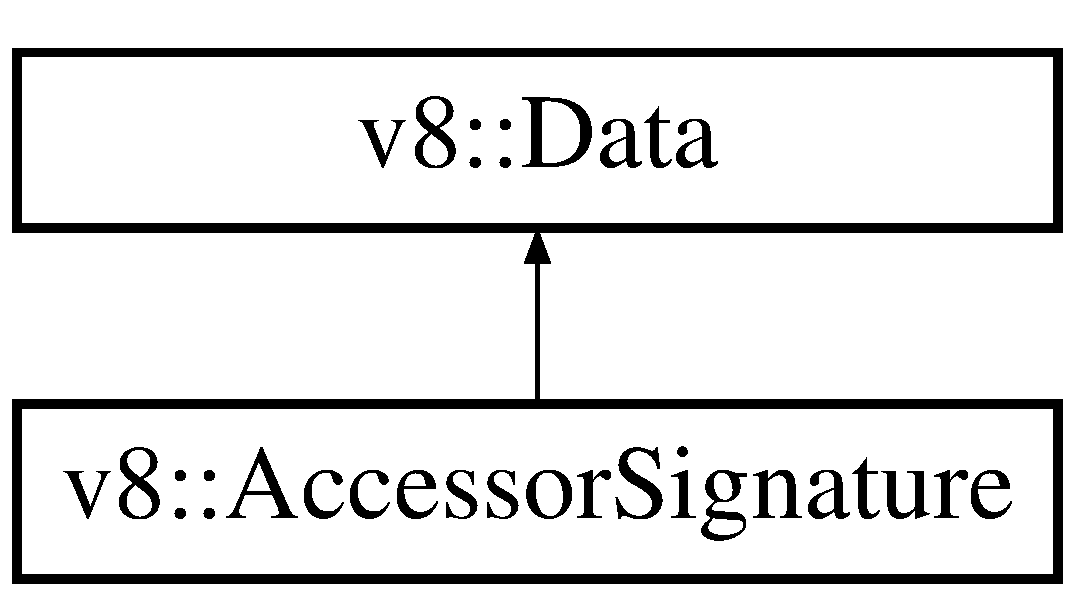
\includegraphics[height=2.000000cm]{classv8_1_1_accessor_signature}
\end{center}
\end{figure}
\subsection*{Static Public Member Functions}
\begin{DoxyCompactItemize}
\item 
static \hyperlink{classv8_1_1_local}{Local}$<$ \hyperlink{classv8_1_1_accessor_signature}{Accessor\+Signature} $>$ {\bfseries New} (\hyperlink{classv8_1_1_isolate}{Isolate} $\ast$isolate, \hyperlink{classv8_1_1_local}{Local}$<$ \hyperlink{classv8_1_1_function_template}{Function\+Template} $>$ receiver=\hyperlink{classv8_1_1_local}{Local}$<$ \hyperlink{classv8_1_1_function_template}{Function\+Template} $>$())\hypertarget{classv8_1_1_accessor_signature_a2d7f28b404be5ecdb501aaf572a7ee52}{}\label{classv8_1_1_accessor_signature_a2d7f28b404be5ecdb501aaf572a7ee52}

\end{DoxyCompactItemize}


\subsection{Detailed Description}
An \hyperlink{classv8_1_1_accessor_signature}{Accessor\+Signature} specifies which receivers are valid parameters to an accessor callback. 

The documentation for this class was generated from the following file\+:\begin{DoxyCompactItemize}
\item 
/\+Users/joshgav/node/v8/include/v8.\+h\end{DoxyCompactItemize}

\hypertarget{classv8_1_1_activity_control}{}\section{v8\+:\+:Activity\+Control Class Reference}
\label{classv8_1_1_activity_control}\index{v8\+::\+Activity\+Control@{v8\+::\+Activity\+Control}}


{\ttfamily \#include $<$v8-\/profiler.\+h$>$}

\subsection*{Public Types}
\begin{DoxyCompactItemize}
\item 
enum {\bfseries Control\+Option} \{ \\*
{\bfseries k\+Continue} = 0, 
\\*
{\bfseries k\+Abort} = 1
 \}\hypertarget{classv8_1_1_activity_control_a6d261e8c21e8076ce86b4add231a8ef9}{}\label{classv8_1_1_activity_control_a6d261e8c21e8076ce86b4add231a8ef9}

\end{DoxyCompactItemize}
\subsection*{Public Member Functions}
\begin{DoxyCompactItemize}
\item 
virtual Control\+Option \hyperlink{classv8_1_1_activity_control_a1300f10611306a3e8f79239e057eb0bf}{Report\+Progress\+Value} (int done, int total)=0
\end{DoxyCompactItemize}


\subsection{Detailed Description}
An interface for reporting progress and controlling long-\/running activities. 

\subsection{Member Function Documentation}
\index{v8\+::\+Activity\+Control@{v8\+::\+Activity\+Control}!Report\+Progress\+Value@{Report\+Progress\+Value}}
\index{Report\+Progress\+Value@{Report\+Progress\+Value}!v8\+::\+Activity\+Control@{v8\+::\+Activity\+Control}}
\subsubsection[{\texorpdfstring{Report\+Progress\+Value(int done, int total)=0}{ReportProgressValue(int done, int total)=0}}]{\setlength{\rightskip}{0pt plus 5cm}virtual Control\+Option v8\+::\+Activity\+Control\+::\+Report\+Progress\+Value (
\begin{DoxyParamCaption}
\item[{int}]{done, }
\item[{int}]{total}
\end{DoxyParamCaption}
)\hspace{0.3cm}{\ttfamily [pure virtual]}}\hypertarget{classv8_1_1_activity_control_a1300f10611306a3e8f79239e057eb0bf}{}\label{classv8_1_1_activity_control_a1300f10611306a3e8f79239e057eb0bf}
Notify about current progress. The activity can be stopped by returning k\+Abort as the callback result. 

The documentation for this class was generated from the following file\+:\begin{DoxyCompactItemize}
\item 
/\+Users/joshgav/node/v8/include/v8-\/profiler.\+h\end{DoxyCompactItemize}

\hypertarget{classv8_1_1_align_of_helper}{}\section{v8\+:\+:Align\+Of\+Helper$<$ T $>$ Class Template Reference}
\label{classv8_1_1_align_of_helper}\index{v8\+::\+Align\+Of\+Helper$<$ T $>$@{v8\+::\+Align\+Of\+Helper$<$ T $>$}}
\subsection*{Private Attributes}
\begin{DoxyCompactItemize}
\item 
char {\bfseries c}\hypertarget{classv8_1_1_align_of_helper_ac23697d1381684b3f4a53f8ff0f29897}{}\label{classv8_1_1_align_of_helper_ac23697d1381684b3f4a53f8ff0f29897}

\item 
T {\bfseries t}\hypertarget{classv8_1_1_align_of_helper_aebba37d9841cf6fb72eaf24e2ba9e33a}{}\label{classv8_1_1_align_of_helper_aebba37d9841cf6fb72eaf24e2ba9e33a}

\end{DoxyCompactItemize}


The documentation for this class was generated from the following file\+:\begin{DoxyCompactItemize}
\item 
include/v8config.\+h\end{DoxyCompactItemize}

\hypertarget{structv8_1_1_allocation_profile_1_1_allocation}{}\section{v8\+:\+:Allocation\+Profile\+:\+:Allocation Struct Reference}
\label{structv8_1_1_allocation_profile_1_1_allocation}\index{v8\+::\+Allocation\+Profile\+::\+Allocation@{v8\+::\+Allocation\+Profile\+::\+Allocation}}
\subsection*{Public Attributes}
\begin{DoxyCompactItemize}
\item 
size\+\_\+t \hyperlink{structv8_1_1_allocation_profile_1_1_allocation_a346410fa5dfb796dff396069897c0aba}{size}
\item 
unsigned int \hyperlink{structv8_1_1_allocation_profile_1_1_allocation_a012fe5238f5ebec039d7832f2d3ae8ed}{count}
\end{DoxyCompactItemize}


\subsection{Member Data Documentation}
\index{v8\+::\+Allocation\+Profile\+::\+Allocation@{v8\+::\+Allocation\+Profile\+::\+Allocation}!count@{count}}
\index{count@{count}!v8\+::\+Allocation\+Profile\+::\+Allocation@{v8\+::\+Allocation\+Profile\+::\+Allocation}}
\subsubsection[{\texorpdfstring{count}{count}}]{\setlength{\rightskip}{0pt plus 5cm}unsigned int v8\+::\+Allocation\+Profile\+::\+Allocation\+::count}\hypertarget{structv8_1_1_allocation_profile_1_1_allocation_a012fe5238f5ebec039d7832f2d3ae8ed}{}\label{structv8_1_1_allocation_profile_1_1_allocation_a012fe5238f5ebec039d7832f2d3ae8ed}
The number of objects of such size that were sampled. \index{v8\+::\+Allocation\+Profile\+::\+Allocation@{v8\+::\+Allocation\+Profile\+::\+Allocation}!size@{size}}
\index{size@{size}!v8\+::\+Allocation\+Profile\+::\+Allocation@{v8\+::\+Allocation\+Profile\+::\+Allocation}}
\subsubsection[{\texorpdfstring{size}{size}}]{\setlength{\rightskip}{0pt plus 5cm}size\+\_\+t v8\+::\+Allocation\+Profile\+::\+Allocation\+::size}\hypertarget{structv8_1_1_allocation_profile_1_1_allocation_a346410fa5dfb796dff396069897c0aba}{}\label{structv8_1_1_allocation_profile_1_1_allocation_a346410fa5dfb796dff396069897c0aba}
Size of the sampled allocation object. 

The documentation for this struct was generated from the following file\+:\begin{DoxyCompactItemize}
\item 
include/v8-\/profiler.\+h\end{DoxyCompactItemize}

\hypertarget{classv8_1_1_allocation_profile}{}\section{v8\+:\+:Allocation\+Profile Class Reference}
\label{classv8_1_1_allocation_profile}\index{v8\+::\+Allocation\+Profile@{v8\+::\+Allocation\+Profile}}


{\ttfamily \#include $<$v8-\/profiler.\+h$>$}

Inheritance diagram for v8\+:\+:Allocation\+Profile\+:\begin{figure}[H]
\begin{center}
\leavevmode
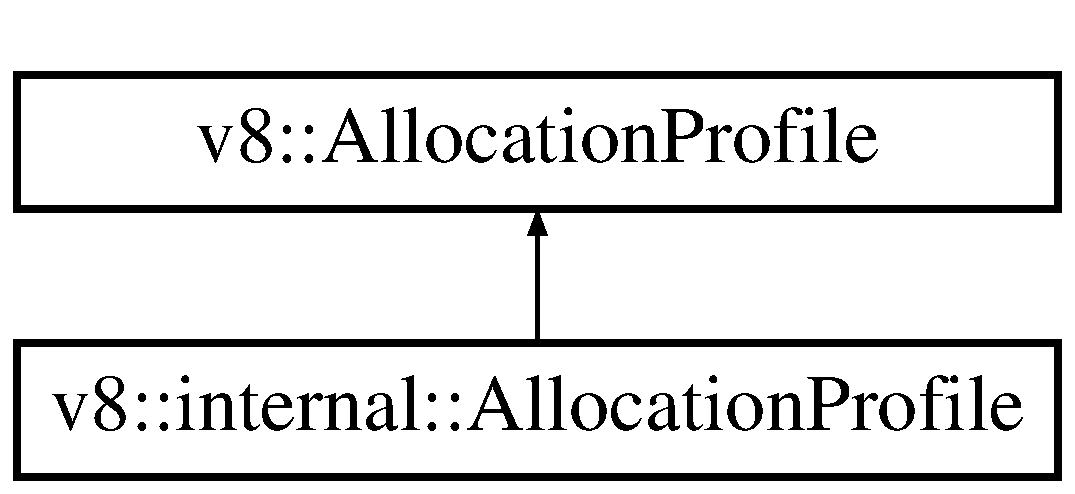
\includegraphics[height=2.000000cm]{classv8_1_1_allocation_profile}
\end{center}
\end{figure}
\subsection*{Classes}
\begin{DoxyCompactItemize}
\item 
struct \hyperlink{structv8_1_1_allocation_profile_1_1_allocation}{Allocation}
\item 
struct \hyperlink{structv8_1_1_allocation_profile_1_1_node}{Node}
\end{DoxyCompactItemize}
\subsection*{Public Member Functions}
\begin{DoxyCompactItemize}
\item 
virtual \hyperlink{structv8_1_1_allocation_profile_1_1_node}{Node} $\ast$ \hyperlink{classv8_1_1_allocation_profile_afea045dae30df5477088e2f0b7edb6c4}{Get\+Root\+Node} ()=0
\end{DoxyCompactItemize}
\subsection*{Static Public Attributes}
\begin{DoxyCompactItemize}
\item 
static const int {\bfseries k\+No\+Line\+Number\+Info} = Message\+::k\+No\+Line\+Number\+Info\hypertarget{classv8_1_1_allocation_profile_a26fdfe9e4846d26c83d0ad8c2ed2d783}{}\label{classv8_1_1_allocation_profile_a26fdfe9e4846d26c83d0ad8c2ed2d783}

\item 
static const int {\bfseries k\+No\+Column\+Number\+Info} = Message\+::k\+No\+Column\+Info\hypertarget{classv8_1_1_allocation_profile_a9cfa103f73e82629694eee3734826eb7}{}\label{classv8_1_1_allocation_profile_a9cfa103f73e82629694eee3734826eb7}

\end{DoxyCompactItemize}


\subsection{Detailed Description}
\hyperlink{classv8_1_1_allocation_profile}{Allocation\+Profile} is a sampled profile of allocations done by the program. This is structured as a call-\/graph. 

\subsection{Member Function Documentation}
\index{v8\+::\+Allocation\+Profile@{v8\+::\+Allocation\+Profile}!Get\+Root\+Node@{Get\+Root\+Node}}
\index{Get\+Root\+Node@{Get\+Root\+Node}!v8\+::\+Allocation\+Profile@{v8\+::\+Allocation\+Profile}}
\subsubsection[{\texorpdfstring{Get\+Root\+Node()=0}{GetRootNode()=0}}]{\setlength{\rightskip}{0pt plus 5cm}virtual {\bf Node}$\ast$ v8\+::\+Allocation\+Profile\+::\+Get\+Root\+Node (
\begin{DoxyParamCaption}
{}
\end{DoxyParamCaption}
)\hspace{0.3cm}{\ttfamily [pure virtual]}}\hypertarget{classv8_1_1_allocation_profile_afea045dae30df5477088e2f0b7edb6c4}{}\label{classv8_1_1_allocation_profile_afea045dae30df5477088e2f0b7edb6c4}
Returns the root node of the call-\/graph. The root node corresponds to an empty JS call-\/stack. The lifetime of the returned Node$\ast$ is scoped to the containing \hyperlink{classv8_1_1_allocation_profile}{Allocation\+Profile}. 

Implemented in \hyperlink{classv8_1_1internal_1_1_allocation_profile_abb93406eaccd8b37de3e080d0620bc2b}{v8\+::internal\+::\+Allocation\+Profile}.



The documentation for this class was generated from the following file\+:\begin{DoxyCompactItemize}
\item 
/\+Users/joshgav/node/v8/include/v8-\/profiler.\+h\end{DoxyCompactItemize}

\hypertarget{classv8_1_1_array_buffer_1_1_allocator}{}\section{v8\+:\+:Array\+Buffer\+:\+:Allocator Class Reference}
\label{classv8_1_1_array_buffer_1_1_allocator}\index{v8\+::\+Array\+Buffer\+::\+Allocator@{v8\+::\+Array\+Buffer\+::\+Allocator}}


{\ttfamily \#include $<$v8.\+h$>$}

\subsection*{Public Member Functions}
\begin{DoxyCompactItemize}
\item 
virtual void $\ast$ \hyperlink{classv8_1_1_array_buffer_1_1_allocator_a106b0d80120ed04fe9b9675e96f0340b}{Allocate} (size\+\_\+t length)=0
\item 
virtual void $\ast$ \hyperlink{classv8_1_1_array_buffer_1_1_allocator_a92b2d5c0a826d3c435e12f3ee178f37a}{Allocate\+Uninitialized} (size\+\_\+t length)=0
\item 
virtual void \hyperlink{classv8_1_1_array_buffer_1_1_allocator_a419f59d2a103a5a8863809d7977c9cd8}{Free} (void $\ast$data, size\+\_\+t length)=0
\end{DoxyCompactItemize}


\subsection{Detailed Description}
\hyperlink{classv8_1_1_array_buffer_1_1_allocator}{Allocator} that \hyperlink{classv8_1_1_v8}{V8} uses to allocate $\vert$\+Array\+Buffer$\vert$\textquotesingle{}s memory. The allocator is a global \hyperlink{classv8_1_1_v8}{V8} setting. It has to be set via \hyperlink{structv8_1_1_isolate_1_1_create_params}{Isolate\+::\+Create\+Params}.

This A\+PI is experimental and may change significantly. 

\subsection{Member Function Documentation}
\index{v8\+::\+Array\+Buffer\+::\+Allocator@{v8\+::\+Array\+Buffer\+::\+Allocator}!Allocate@{Allocate}}
\index{Allocate@{Allocate}!v8\+::\+Array\+Buffer\+::\+Allocator@{v8\+::\+Array\+Buffer\+::\+Allocator}}
\subsubsection[{\texorpdfstring{Allocate(size\+\_\+t length)=0}{Allocate(size_t length)=0}}]{\setlength{\rightskip}{0pt plus 5cm}virtual void$\ast$ v8\+::\+Array\+Buffer\+::\+Allocator\+::\+Allocate (
\begin{DoxyParamCaption}
\item[{size\+\_\+t}]{length}
\end{DoxyParamCaption}
)\hspace{0.3cm}{\ttfamily [pure virtual]}}\hypertarget{classv8_1_1_array_buffer_1_1_allocator_a106b0d80120ed04fe9b9675e96f0340b}{}\label{classv8_1_1_array_buffer_1_1_allocator_a106b0d80120ed04fe9b9675e96f0340b}
Allocate $\vert$length$\vert$ bytes. Return N\+U\+LL if allocation is not successful. Memory should be initialized to zeroes. \index{v8\+::\+Array\+Buffer\+::\+Allocator@{v8\+::\+Array\+Buffer\+::\+Allocator}!Allocate\+Uninitialized@{Allocate\+Uninitialized}}
\index{Allocate\+Uninitialized@{Allocate\+Uninitialized}!v8\+::\+Array\+Buffer\+::\+Allocator@{v8\+::\+Array\+Buffer\+::\+Allocator}}
\subsubsection[{\texorpdfstring{Allocate\+Uninitialized(size\+\_\+t length)=0}{AllocateUninitialized(size_t length)=0}}]{\setlength{\rightskip}{0pt plus 5cm}virtual void$\ast$ v8\+::\+Array\+Buffer\+::\+Allocator\+::\+Allocate\+Uninitialized (
\begin{DoxyParamCaption}
\item[{size\+\_\+t}]{length}
\end{DoxyParamCaption}
)\hspace{0.3cm}{\ttfamily [pure virtual]}}\hypertarget{classv8_1_1_array_buffer_1_1_allocator_a92b2d5c0a826d3c435e12f3ee178f37a}{}\label{classv8_1_1_array_buffer_1_1_allocator_a92b2d5c0a826d3c435e12f3ee178f37a}
Allocate $\vert$length$\vert$ bytes. Return N\+U\+LL if allocation is not successful. Memory does not have to be initialized. \index{v8\+::\+Array\+Buffer\+::\+Allocator@{v8\+::\+Array\+Buffer\+::\+Allocator}!Free@{Free}}
\index{Free@{Free}!v8\+::\+Array\+Buffer\+::\+Allocator@{v8\+::\+Array\+Buffer\+::\+Allocator}}
\subsubsection[{\texorpdfstring{Free(void $\ast$data, size\+\_\+t length)=0}{Free(void *data, size_t length)=0}}]{\setlength{\rightskip}{0pt plus 5cm}virtual void v8\+::\+Array\+Buffer\+::\+Allocator\+::\+Free (
\begin{DoxyParamCaption}
\item[{void $\ast$}]{data, }
\item[{size\+\_\+t}]{length}
\end{DoxyParamCaption}
)\hspace{0.3cm}{\ttfamily [pure virtual]}}\hypertarget{classv8_1_1_array_buffer_1_1_allocator_a419f59d2a103a5a8863809d7977c9cd8}{}\label{classv8_1_1_array_buffer_1_1_allocator_a419f59d2a103a5a8863809d7977c9cd8}
Free the memory block of size $\vert$length$\vert$, pointed to by $\vert$data$\vert$. That memory is guaranteed to be previously allocated by $\vert$\+Allocate$\vert$. 

The documentation for this class was generated from the following file\+:\begin{DoxyCompactItemize}
\item 
/\+Users/joshgav/node/v8/include/v8.\+h\end{DoxyCompactItemize}

\hypertarget{classv8_1_1_isolate_1_1_allow_javascript_execution_scope}{}\section{v8\+:\+:Isolate\+:\+:Allow\+Javascript\+Execution\+Scope Class Reference}
\label{classv8_1_1_isolate_1_1_allow_javascript_execution_scope}\index{v8\+::\+Isolate\+::\+Allow\+Javascript\+Execution\+Scope@{v8\+::\+Isolate\+::\+Allow\+Javascript\+Execution\+Scope}}


{\ttfamily \#include $<$v8.\+h$>$}

\subsection*{Public Member Functions}
\begin{DoxyCompactItemize}
\item 
{\bfseries Allow\+Javascript\+Execution\+Scope} (\hyperlink{classv8_1_1_isolate}{Isolate} $\ast$isolate)\hypertarget{classv8_1_1_isolate_1_1_allow_javascript_execution_scope_ac73a647c33756c6b7c3896170e069e8c}{}\label{classv8_1_1_isolate_1_1_allow_javascript_execution_scope_ac73a647c33756c6b7c3896170e069e8c}

\end{DoxyCompactItemize}
\subsection*{Private Member Functions}
\begin{DoxyCompactItemize}
\item 
{\bfseries Allow\+Javascript\+Execution\+Scope} (const \hyperlink{classv8_1_1_isolate_1_1_allow_javascript_execution_scope}{Allow\+Javascript\+Execution\+Scope} \&)\hypertarget{classv8_1_1_isolate_1_1_allow_javascript_execution_scope_a9968118fbefa05ce6cb97373efe32656}{}\label{classv8_1_1_isolate_1_1_allow_javascript_execution_scope_a9968118fbefa05ce6cb97373efe32656}

\item 
\hyperlink{classv8_1_1_isolate_1_1_allow_javascript_execution_scope}{Allow\+Javascript\+Execution\+Scope} \& {\bfseries operator=} (const \hyperlink{classv8_1_1_isolate_1_1_allow_javascript_execution_scope}{Allow\+Javascript\+Execution\+Scope} \&)\hypertarget{classv8_1_1_isolate_1_1_allow_javascript_execution_scope_a4ca08db8ddcb39695011739c31b54349}{}\label{classv8_1_1_isolate_1_1_allow_javascript_execution_scope_a4ca08db8ddcb39695011739c31b54349}

\end{DoxyCompactItemize}
\subsection*{Private Attributes}
\begin{DoxyCompactItemize}
\item 
void $\ast$ {\bfseries internal\+\_\+throws\+\_\+}\hypertarget{classv8_1_1_isolate_1_1_allow_javascript_execution_scope_a991c6fdbad58aae983e2107de2423f80}{}\label{classv8_1_1_isolate_1_1_allow_javascript_execution_scope_a991c6fdbad58aae983e2107de2423f80}

\item 
void $\ast$ {\bfseries internal\+\_\+assert\+\_\+}\hypertarget{classv8_1_1_isolate_1_1_allow_javascript_execution_scope_a5ef196e5ce1c7c3602b3bbe4674dab3c}{}\label{classv8_1_1_isolate_1_1_allow_javascript_execution_scope_a5ef196e5ce1c7c3602b3bbe4674dab3c}

\end{DoxyCompactItemize}


\subsection{Detailed Description}
Introduce exception to \hyperlink{classv8_1_1_isolate_1_1_disallow_javascript_execution_scope}{Disallow\+Javascript\+Execution\+Scope}. 

The documentation for this class was generated from the following file\+:\begin{DoxyCompactItemize}
\item 
/\+Users/joshgav/node/v8/include/v8.\+h\end{DoxyCompactItemize}

\hypertarget{classv8_1_1_array}{}\section{v8\+:\+:Array Class Reference}
\label{classv8_1_1_array}\index{v8\+::\+Array@{v8\+::\+Array}}


{\ttfamily \#include $<$v8.\+h$>$}

Inheritance diagram for v8\+:\+:Array\+:\begin{figure}[H]
\begin{center}
\leavevmode
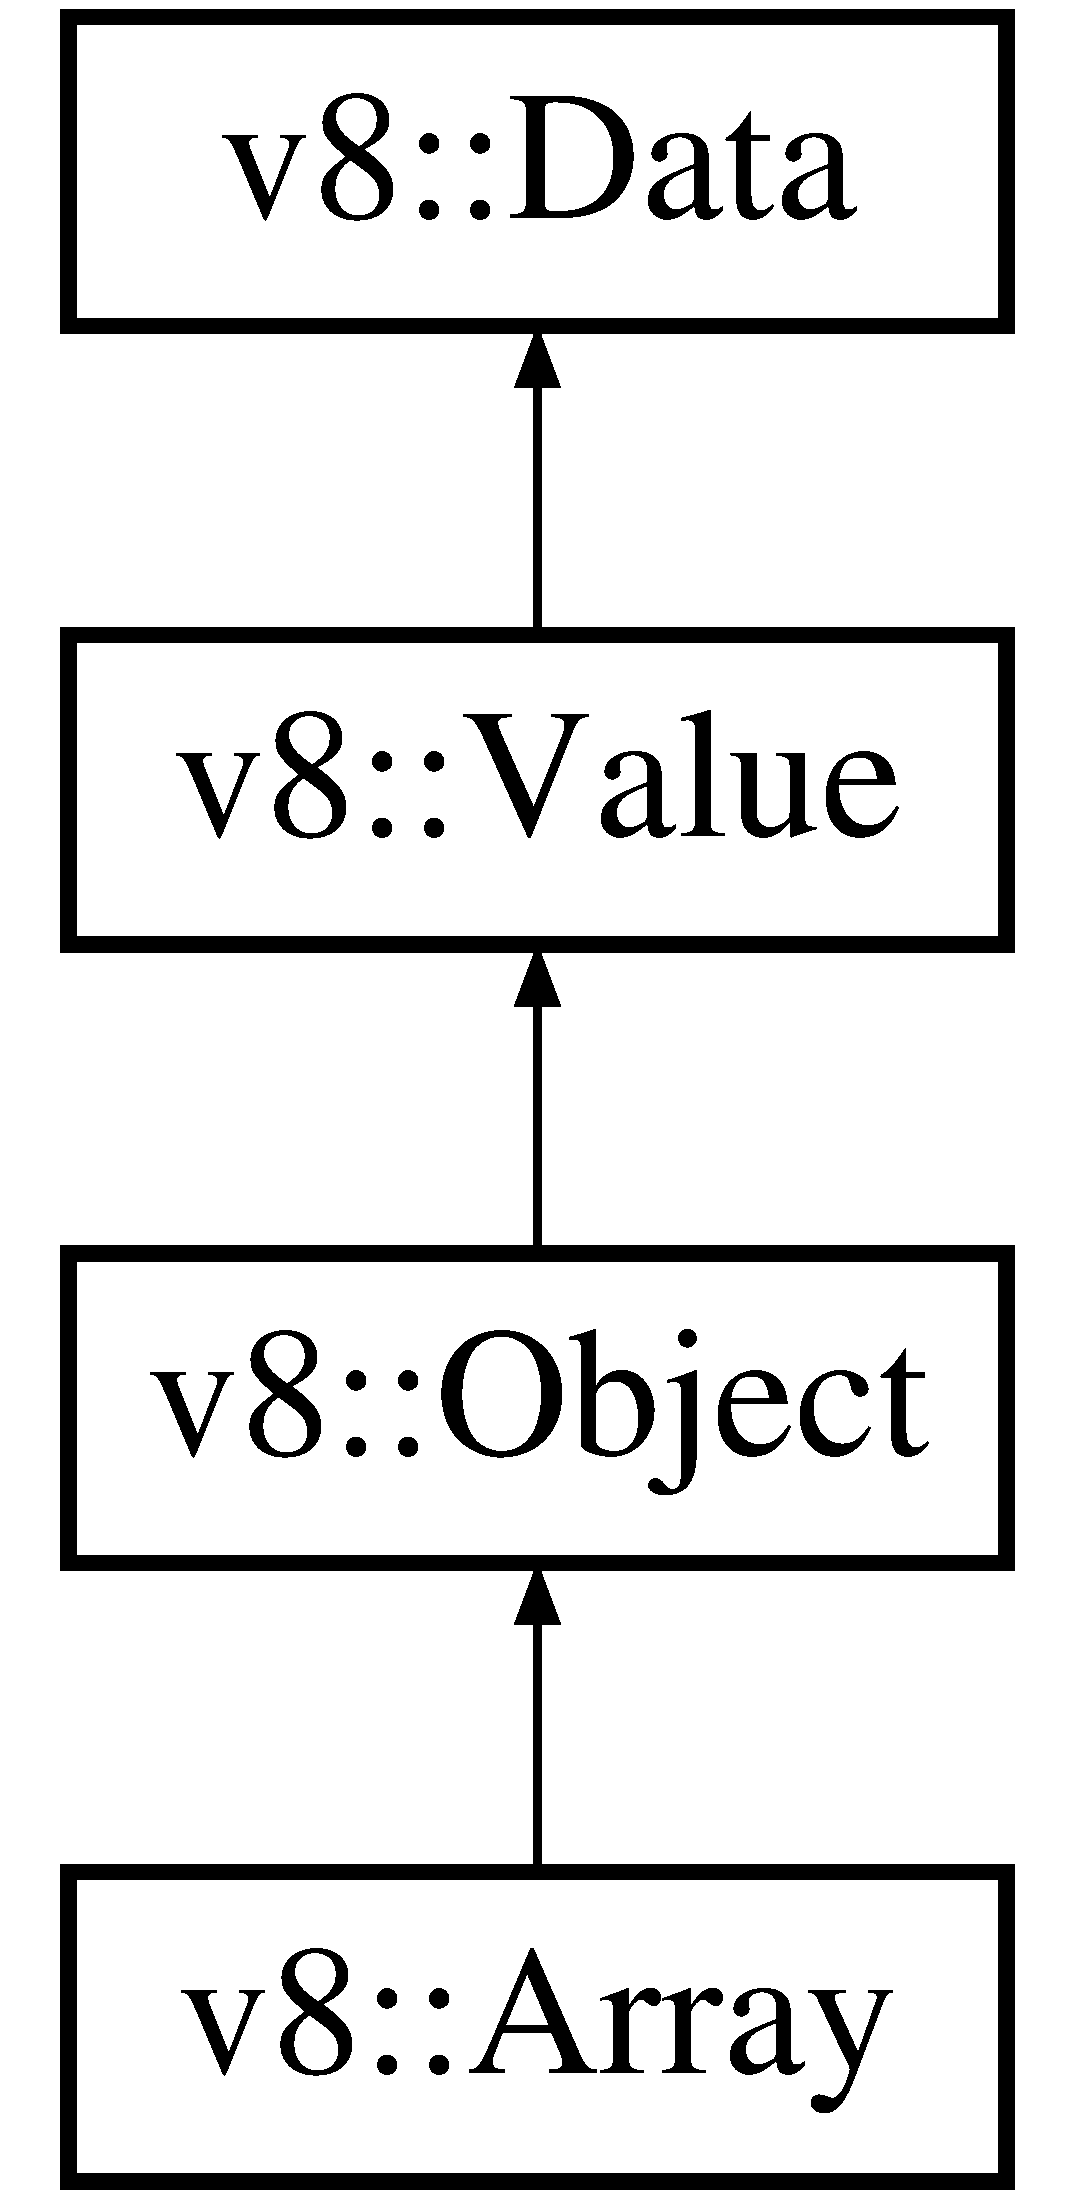
\includegraphics[height=4.000000cm]{classv8_1_1_array}
\end{center}
\end{figure}
\subsection*{Public Member Functions}
\begin{DoxyCompactItemize}
\item 
uint32\+\_\+t {\bfseries Length} () const \hypertarget{classv8_1_1_array_a3c47dfd8d26e60ed4fcdc683034d6d9c}{}\label{classv8_1_1_array_a3c47dfd8d26e60ed4fcdc683034d6d9c}

\item 
\hyperlink{classv8_1_1_array_ae4d15fb9781bcd653e5eecffd4d0ffac}{V8\+\_\+\+D\+E\+P\+R\+E\+C\+A\+T\+ED} (\char`\"{}Cloning is not supported.\char`\"{}, Local$<$ \hyperlink{classv8_1_1_object}{Object} $>$ Clone\+Element\+At(uint32\+\_\+t index))
\item 
{\bfseries V8\+\_\+\+D\+E\+P\+R\+E\+C\+A\+T\+ED} (\char`\"{}Cloning is not supported.\char`\"{}, Maybe\+Local$<$ \hyperlink{classv8_1_1_object}{Object} $>$ Clone\+Element\+At(\hyperlink{classv8_1_1_local}{Local}$<$ \hyperlink{classv8_1_1_context}{Context} $>$ context,                                                                                                                                                                                               uint32\+\_\+t index))\hypertarget{classv8_1_1_array_ae30e4a34fc94cd4b52cd21d508b6e3b7}{}\label{classv8_1_1_array_ae30e4a34fc94cd4b52cd21d508b6e3b7}

\end{DoxyCompactItemize}
\subsection*{Static Public Member Functions}
\begin{DoxyCompactItemize}
\item 
static \hyperlink{classv8_1_1_local}{Local}$<$ \hyperlink{classv8_1_1_array}{Array} $>$ \hyperlink{classv8_1_1_array_a892f18fe6a25dfc0bc7b435759a30226}{New} (\hyperlink{classv8_1_1_isolate}{Isolate} $\ast$isolate, int length=0)
\item 
static V8\+\_\+\+I\+N\+L\+I\+NE \hyperlink{classv8_1_1_array}{Array} $\ast$ {\bfseries Cast} (\hyperlink{classv8_1_1_value}{Value} $\ast$obj)\hypertarget{classv8_1_1_array_ae56792766f8513395c3ebe8c29afde4b}{}\label{classv8_1_1_array_ae56792766f8513395c3ebe8c29afde4b}

\end{DoxyCompactItemize}
\subsection*{Static Private Member Functions}
\begin{DoxyCompactItemize}
\item 
static void {\bfseries Check\+Cast} (\hyperlink{classv8_1_1_value}{Value} $\ast$obj)\hypertarget{classv8_1_1_array_af0b37e9453a594b16c7f6ad2c07b11ac}{}\label{classv8_1_1_array_af0b37e9453a594b16c7f6ad2c07b11ac}

\end{DoxyCompactItemize}


\subsection{Detailed Description}
An instance of the built-\/in array constructor (E\+C\+M\+A-\/262, 15.\+4.\+2). 

\subsection{Member Function Documentation}
\index{v8\+::\+Array@{v8\+::\+Array}!New@{New}}
\index{New@{New}!v8\+::\+Array@{v8\+::\+Array}}
\subsubsection[{\texorpdfstring{New(\+Isolate $\ast$isolate, int length=0)}{New(Isolate *isolate, int length=0)}}]{\setlength{\rightskip}{0pt plus 5cm}static {\bf Local}$<${\bf Array}$>$ v8\+::\+Array\+::\+New (
\begin{DoxyParamCaption}
\item[{{\bf Isolate} $\ast$}]{isolate, }
\item[{int}]{length = {\ttfamily 0}}
\end{DoxyParamCaption}
)\hspace{0.3cm}{\ttfamily [static]}}\hypertarget{classv8_1_1_array_a892f18fe6a25dfc0bc7b435759a30226}{}\label{classv8_1_1_array_a892f18fe6a25dfc0bc7b435759a30226}
Creates a Java\+Script array with the given length. If the length is negative the returned array will have length 0. \index{v8\+::\+Array@{v8\+::\+Array}!V8\+\_\+\+D\+E\+P\+R\+E\+C\+A\+T\+ED@{V8\+\_\+\+D\+E\+P\+R\+E\+C\+A\+T\+ED}}
\index{V8\+\_\+\+D\+E\+P\+R\+E\+C\+A\+T\+ED@{V8\+\_\+\+D\+E\+P\+R\+E\+C\+A\+T\+ED}!v8\+::\+Array@{v8\+::\+Array}}
\subsubsection[{\texorpdfstring{V8\+\_\+\+D\+E\+P\+R\+E\+C\+A\+T\+E\+D(""Cloning is not supported."", Local$<$ Object $>$ Clone\+Element\+At(uint32\+\_\+t index))}{V8_DEPRECATED("Cloning is not supported.", Local< Object > CloneElementAt(uint32_t index))}}]{\setlength{\rightskip}{0pt plus 5cm}v8\+::\+Array\+::\+V8\+\_\+\+D\+E\+P\+R\+E\+C\+A\+T\+ED (
\begin{DoxyParamCaption}
\item[{\char`\"{}Cloning is not supported.\char`\"{}}]{, }
\item[{{\bf Local}$<$ {\bf Object} $>$ }]{Clone\+Element\+Atuint32\+\_\+t index}
\end{DoxyParamCaption}
)}\hypertarget{classv8_1_1_array_ae4d15fb9781bcd653e5eecffd4d0ffac}{}\label{classv8_1_1_array_ae4d15fb9781bcd653e5eecffd4d0ffac}
Clones an element at index $\vert$index$\vert$. Returns an empty handle if cloning fails (for any reason). 

The documentation for this class was generated from the following file\+:\begin{DoxyCompactItemize}
\item 
include/v8.\+h\end{DoxyCompactItemize}

\hypertarget{classv8_1_1_array_buffer}{}\section{v8\+:\+:Array\+Buffer Class Reference}
\label{classv8_1_1_array_buffer}\index{v8\+::\+Array\+Buffer@{v8\+::\+Array\+Buffer}}


{\ttfamily \#include $<$v8.\+h$>$}

Inheritance diagram for v8\+:\+:Array\+Buffer\+:\begin{figure}[H]
\begin{center}
\leavevmode
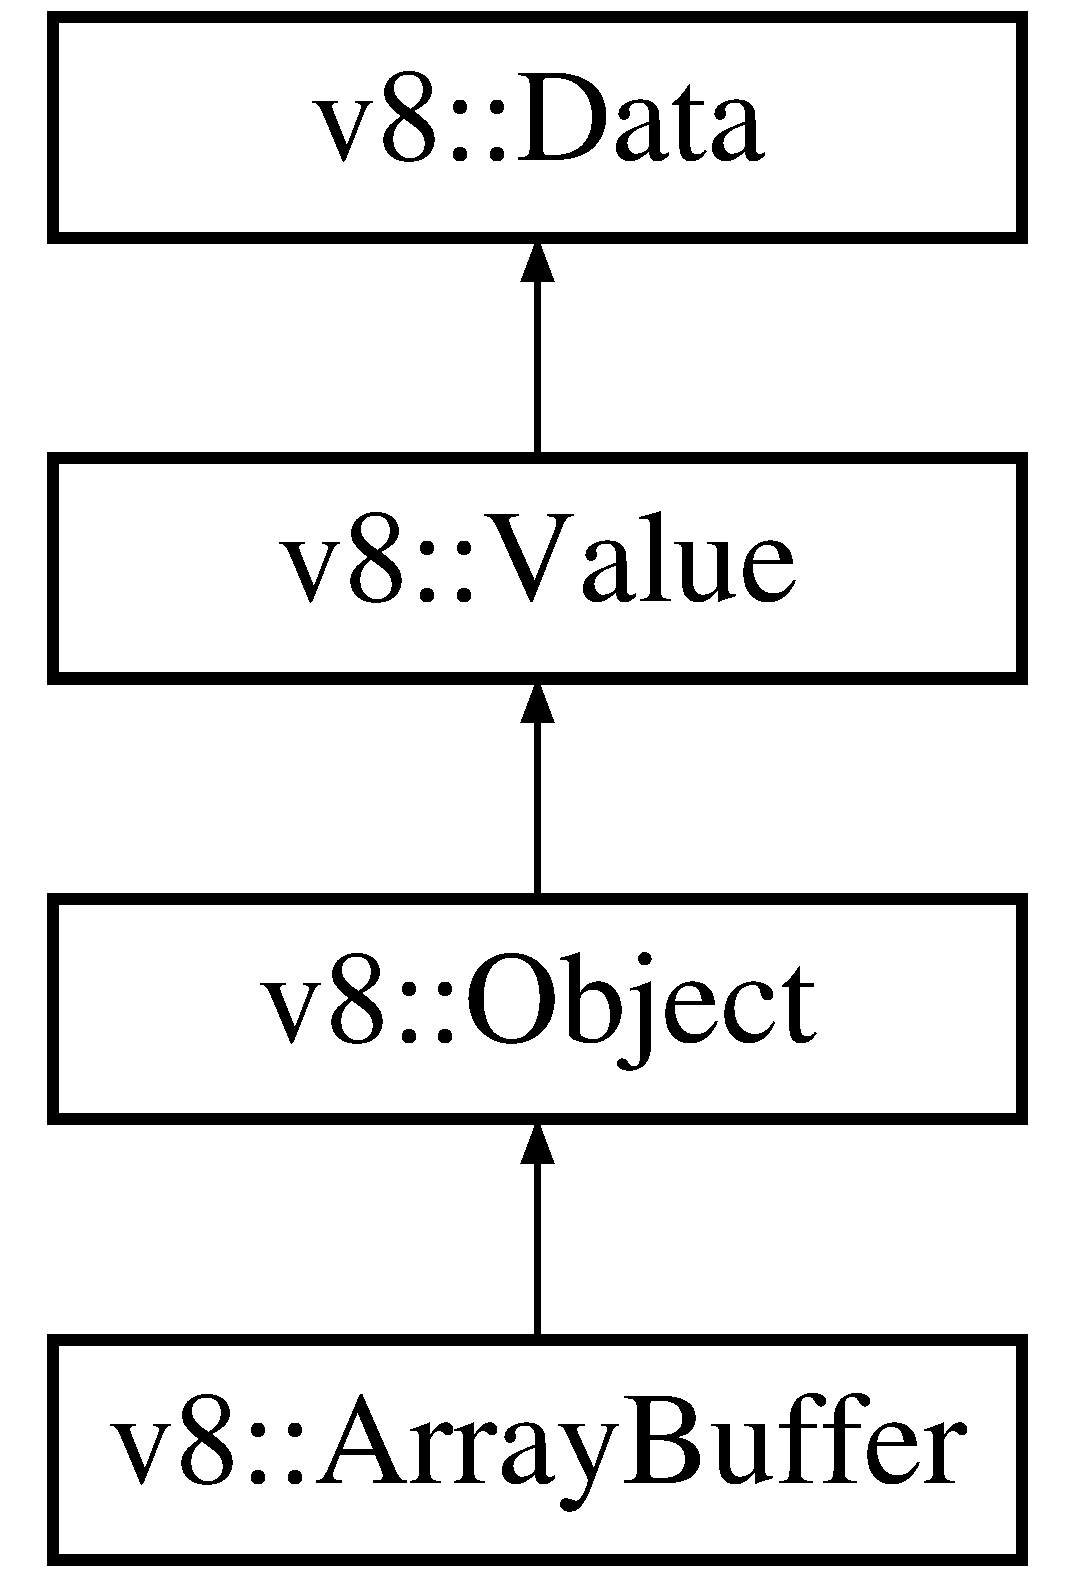
\includegraphics[height=4.000000cm]{classv8_1_1_array_buffer}
\end{center}
\end{figure}
\subsection*{Classes}
\begin{DoxyCompactItemize}
\item 
class \hyperlink{classv8_1_1_array_buffer_1_1_allocator}{Allocator}
\item 
class \hyperlink{classv8_1_1_array_buffer_1_1_contents}{Contents}
\end{DoxyCompactItemize}
\subsection*{Public Member Functions}
\begin{DoxyCompactItemize}
\item 
size\+\_\+t \hyperlink{classv8_1_1_array_buffer_ab73b98ba6436b57c5a1b3d29429e0199}{Byte\+Length} () const 
\item 
bool \hyperlink{classv8_1_1_array_buffer_a50dd263917559439525048c623425c6f}{Is\+External} () const 
\item 
bool \hyperlink{classv8_1_1_array_buffer_aed177cd83c3368837f740fa2929b3c8d}{Is\+Neuterable} () const 
\item 
void \hyperlink{classv8_1_1_array_buffer_a3420f7d38a8fe20e8f40fb82e6acb325}{Neuter} ()
\item 
\hyperlink{classv8_1_1_array_buffer_1_1_contents}{Contents} \hyperlink{classv8_1_1_array_buffer_a8b90b72486cfacb4fbec157f4803f889}{Externalize} ()
\item 
\hyperlink{classv8_1_1_array_buffer_1_1_contents}{Contents} \hyperlink{classv8_1_1_array_buffer_ae44291df12ca35de9b519e7372aa640a}{Get\+Contents} ()
\end{DoxyCompactItemize}
\subsection*{Static Public Member Functions}
\begin{DoxyCompactItemize}
\item 
static \hyperlink{classv8_1_1_local}{Local}$<$ \hyperlink{classv8_1_1_array_buffer}{Array\+Buffer} $>$ \hyperlink{classv8_1_1_array_buffer_ad752e03d7cc7fe863656ad6183785ab7}{New} (\hyperlink{classv8_1_1_isolate}{Isolate} $\ast$isolate, size\+\_\+t byte\+\_\+length)
\item 
static \hyperlink{classv8_1_1_local}{Local}$<$ \hyperlink{classv8_1_1_array_buffer}{Array\+Buffer} $>$ \hyperlink{classv8_1_1_array_buffer_acc65e714766b0d0d791b0d43ec52d0bb}{New} (\hyperlink{classv8_1_1_isolate}{Isolate} $\ast$isolate, void $\ast$data, size\+\_\+t byte\+\_\+length, Array\+Buffer\+Creation\+Mode mode=Array\+Buffer\+Creation\+Mode\+::k\+Externalized)
\item 
static V8\+\_\+\+I\+N\+L\+I\+NE \hyperlink{classv8_1_1_array_buffer}{Array\+Buffer} $\ast$ {\bfseries Cast} (\hyperlink{classv8_1_1_value}{Value} $\ast$obj)\hypertarget{classv8_1_1_array_buffer_a4b0a703ae34217507a8ebc9cabf7336a}{}\label{classv8_1_1_array_buffer_a4b0a703ae34217507a8ebc9cabf7336a}

\end{DoxyCompactItemize}
\subsection*{Static Public Attributes}
\begin{DoxyCompactItemize}
\item 
static const int {\bfseries k\+Internal\+Field\+Count} = V8\+\_\+\+A\+R\+R\+A\+Y\+\_\+\+B\+U\+F\+F\+E\+R\+\_\+\+I\+N\+T\+E\+R\+N\+A\+L\+\_\+\+F\+I\+E\+L\+D\+\_\+\+C\+O\+U\+NT\hypertarget{classv8_1_1_array_buffer_af49000a2ea120e49da846ef02a42ac69}{}\label{classv8_1_1_array_buffer_af49000a2ea120e49da846ef02a42ac69}

\end{DoxyCompactItemize}
\subsection*{Static Private Member Functions}
\begin{DoxyCompactItemize}
\item 
static void {\bfseries Check\+Cast} (\hyperlink{classv8_1_1_value}{Value} $\ast$obj)\hypertarget{classv8_1_1_array_buffer_af22a450a92f781cbf0dbac30ac560a3c}{}\label{classv8_1_1_array_buffer_af22a450a92f781cbf0dbac30ac560a3c}

\end{DoxyCompactItemize}


\subsection{Detailed Description}
An instance of the built-\/in \hyperlink{classv8_1_1_array_buffer}{Array\+Buffer} constructor (E\+S6 draft 15.\+13.\+5). This A\+PI is experimental and may change significantly. 

\subsection{Member Function Documentation}
\index{v8\+::\+Array\+Buffer@{v8\+::\+Array\+Buffer}!Byte\+Length@{Byte\+Length}}
\index{Byte\+Length@{Byte\+Length}!v8\+::\+Array\+Buffer@{v8\+::\+Array\+Buffer}}
\subsubsection[{\texorpdfstring{Byte\+Length() const }{ByteLength() const }}]{\setlength{\rightskip}{0pt plus 5cm}size\+\_\+t v8\+::\+Array\+Buffer\+::\+Byte\+Length (
\begin{DoxyParamCaption}
{}
\end{DoxyParamCaption}
) const}\hypertarget{classv8_1_1_array_buffer_ab73b98ba6436b57c5a1b3d29429e0199}{}\label{classv8_1_1_array_buffer_ab73b98ba6436b57c5a1b3d29429e0199}
\hyperlink{classv8_1_1_data}{Data} length in bytes. \index{v8\+::\+Array\+Buffer@{v8\+::\+Array\+Buffer}!Externalize@{Externalize}}
\index{Externalize@{Externalize}!v8\+::\+Array\+Buffer@{v8\+::\+Array\+Buffer}}
\subsubsection[{\texorpdfstring{Externalize()}{Externalize()}}]{\setlength{\rightskip}{0pt plus 5cm}{\bf Contents} v8\+::\+Array\+Buffer\+::\+Externalize (
\begin{DoxyParamCaption}
{}
\end{DoxyParamCaption}
)}\hypertarget{classv8_1_1_array_buffer_a8b90b72486cfacb4fbec157f4803f889}{}\label{classv8_1_1_array_buffer_a8b90b72486cfacb4fbec157f4803f889}
Make this \hyperlink{classv8_1_1_array_buffer}{Array\+Buffer} external. The pointer to underlying memory block and byte length are returned as $\vert$\+Contents$\vert$ structure. After \hyperlink{classv8_1_1_array_buffer}{Array\+Buffer} had been etxrenalized, it does no longer owns the memory block. The caller should take steps to free memory when it is no longer needed.

The memory block is guaranteed to be allocated with $\vert$\+Allocator\+::\+Allocate$\vert$ that has been set via \hyperlink{structv8_1_1_isolate_1_1_create_params}{Isolate\+::\+Create\+Params}. \index{v8\+::\+Array\+Buffer@{v8\+::\+Array\+Buffer}!Get\+Contents@{Get\+Contents}}
\index{Get\+Contents@{Get\+Contents}!v8\+::\+Array\+Buffer@{v8\+::\+Array\+Buffer}}
\subsubsection[{\texorpdfstring{Get\+Contents()}{GetContents()}}]{\setlength{\rightskip}{0pt plus 5cm}{\bf Contents} v8\+::\+Array\+Buffer\+::\+Get\+Contents (
\begin{DoxyParamCaption}
{}
\end{DoxyParamCaption}
)}\hypertarget{classv8_1_1_array_buffer_ae44291df12ca35de9b519e7372aa640a}{}\label{classv8_1_1_array_buffer_ae44291df12ca35de9b519e7372aa640a}
Get a pointer to the \hyperlink{classv8_1_1_array_buffer}{Array\+Buffer}\textquotesingle{}s underlying memory block without externalizing it. If the \hyperlink{classv8_1_1_array_buffer}{Array\+Buffer} is not externalized, this pointer will become invalid as soon as the \hyperlink{classv8_1_1_array_buffer}{Array\+Buffer} became garbage collected.

The embedder should make sure to hold a strong reference to the \hyperlink{classv8_1_1_array_buffer}{Array\+Buffer} while accessing this pointer.

The memory block is guaranteed to be allocated with $\vert$\+Allocator\+::\+Allocate$\vert$. \index{v8\+::\+Array\+Buffer@{v8\+::\+Array\+Buffer}!Is\+External@{Is\+External}}
\index{Is\+External@{Is\+External}!v8\+::\+Array\+Buffer@{v8\+::\+Array\+Buffer}}
\subsubsection[{\texorpdfstring{Is\+External() const }{IsExternal() const }}]{\setlength{\rightskip}{0pt plus 5cm}bool v8\+::\+Array\+Buffer\+::\+Is\+External (
\begin{DoxyParamCaption}
{}
\end{DoxyParamCaption}
) const}\hypertarget{classv8_1_1_array_buffer_a50dd263917559439525048c623425c6f}{}\label{classv8_1_1_array_buffer_a50dd263917559439525048c623425c6f}
Returns true if \hyperlink{classv8_1_1_array_buffer}{Array\+Buffer} is externalized, that is, does not own its memory block. \index{v8\+::\+Array\+Buffer@{v8\+::\+Array\+Buffer}!Is\+Neuterable@{Is\+Neuterable}}
\index{Is\+Neuterable@{Is\+Neuterable}!v8\+::\+Array\+Buffer@{v8\+::\+Array\+Buffer}}
\subsubsection[{\texorpdfstring{Is\+Neuterable() const }{IsNeuterable() const }}]{\setlength{\rightskip}{0pt plus 5cm}bool v8\+::\+Array\+Buffer\+::\+Is\+Neuterable (
\begin{DoxyParamCaption}
{}
\end{DoxyParamCaption}
) const}\hypertarget{classv8_1_1_array_buffer_aed177cd83c3368837f740fa2929b3c8d}{}\label{classv8_1_1_array_buffer_aed177cd83c3368837f740fa2929b3c8d}
Returns true if this \hyperlink{classv8_1_1_array_buffer}{Array\+Buffer} may be neutered. \index{v8\+::\+Array\+Buffer@{v8\+::\+Array\+Buffer}!Neuter@{Neuter}}
\index{Neuter@{Neuter}!v8\+::\+Array\+Buffer@{v8\+::\+Array\+Buffer}}
\subsubsection[{\texorpdfstring{Neuter()}{Neuter()}}]{\setlength{\rightskip}{0pt plus 5cm}void v8\+::\+Array\+Buffer\+::\+Neuter (
\begin{DoxyParamCaption}
{}
\end{DoxyParamCaption}
)}\hypertarget{classv8_1_1_array_buffer_a3420f7d38a8fe20e8f40fb82e6acb325}{}\label{classv8_1_1_array_buffer_a3420f7d38a8fe20e8f40fb82e6acb325}
Neuters this \hyperlink{classv8_1_1_array_buffer}{Array\+Buffer} and all its views (typed arrays). Neutering sets the byte length of the buffer and all typed arrays to zero, preventing Java\+Script from ever accessing underlying backing store. \hyperlink{classv8_1_1_array_buffer}{Array\+Buffer} should have been externalized and must be neuterable. \index{v8\+::\+Array\+Buffer@{v8\+::\+Array\+Buffer}!New@{New}}
\index{New@{New}!v8\+::\+Array\+Buffer@{v8\+::\+Array\+Buffer}}
\subsubsection[{\texorpdfstring{New(\+Isolate $\ast$isolate, size\+\_\+t byte\+\_\+length)}{New(Isolate *isolate, size_t byte_length)}}]{\setlength{\rightskip}{0pt plus 5cm}static {\bf Local}$<${\bf Array\+Buffer}$>$ v8\+::\+Array\+Buffer\+::\+New (
\begin{DoxyParamCaption}
\item[{{\bf Isolate} $\ast$}]{isolate, }
\item[{size\+\_\+t}]{byte\+\_\+length}
\end{DoxyParamCaption}
)\hspace{0.3cm}{\ttfamily [static]}}\hypertarget{classv8_1_1_array_buffer_ad752e03d7cc7fe863656ad6183785ab7}{}\label{classv8_1_1_array_buffer_ad752e03d7cc7fe863656ad6183785ab7}
Create a new \hyperlink{classv8_1_1_array_buffer}{Array\+Buffer}. Allocate $\vert$byte\+\_\+length$\vert$ bytes. Allocated memory will be owned by a created \hyperlink{classv8_1_1_array_buffer}{Array\+Buffer} and will be deallocated when it is garbage-\/collected, unless the object is externalized. \index{v8\+::\+Array\+Buffer@{v8\+::\+Array\+Buffer}!New@{New}}
\index{New@{New}!v8\+::\+Array\+Buffer@{v8\+::\+Array\+Buffer}}
\subsubsection[{\texorpdfstring{New(\+Isolate $\ast$isolate, void $\ast$data, size\+\_\+t byte\+\_\+length, Array\+Buffer\+Creation\+Mode mode=\+Array\+Buffer\+Creation\+Mode\+::k\+Externalized)}{New(Isolate *isolate, void *data, size_t byte_length, ArrayBufferCreationMode mode=ArrayBufferCreationMode::kExternalized)}}]{\setlength{\rightskip}{0pt plus 5cm}static {\bf Local}$<${\bf Array\+Buffer}$>$ v8\+::\+Array\+Buffer\+::\+New (
\begin{DoxyParamCaption}
\item[{{\bf Isolate} $\ast$}]{isolate, }
\item[{void $\ast$}]{data, }
\item[{size\+\_\+t}]{byte\+\_\+length, }
\item[{Array\+Buffer\+Creation\+Mode}]{mode = {\ttfamily ArrayBufferCreationMode\+:\+:kExternalized}}
\end{DoxyParamCaption}
)\hspace{0.3cm}{\ttfamily [static]}}\hypertarget{classv8_1_1_array_buffer_acc65e714766b0d0d791b0d43ec52d0bb}{}\label{classv8_1_1_array_buffer_acc65e714766b0d0d791b0d43ec52d0bb}
Create a new \hyperlink{classv8_1_1_array_buffer}{Array\+Buffer} over an existing memory block. The created array buffer is by default immediately in externalized state. The memory block will not be reclaimed when a created \hyperlink{classv8_1_1_array_buffer}{Array\+Buffer} is garbage-\/collected. 

The documentation for this class was generated from the following file\+:\begin{DoxyCompactItemize}
\item 
/\+Users/joshgav/node/v8/include/v8.\+h\end{DoxyCompactItemize}

\hypertarget{classv8_1_1_array_buffer_view}{}\section{v8\+:\+:Array\+Buffer\+View Class Reference}
\label{classv8_1_1_array_buffer_view}\index{v8\+::\+Array\+Buffer\+View@{v8\+::\+Array\+Buffer\+View}}


{\ttfamily \#include $<$v8.\+h$>$}

Inheritance diagram for v8\+:\+:Array\+Buffer\+View\+:\begin{figure}[H]
\begin{center}
\leavevmode
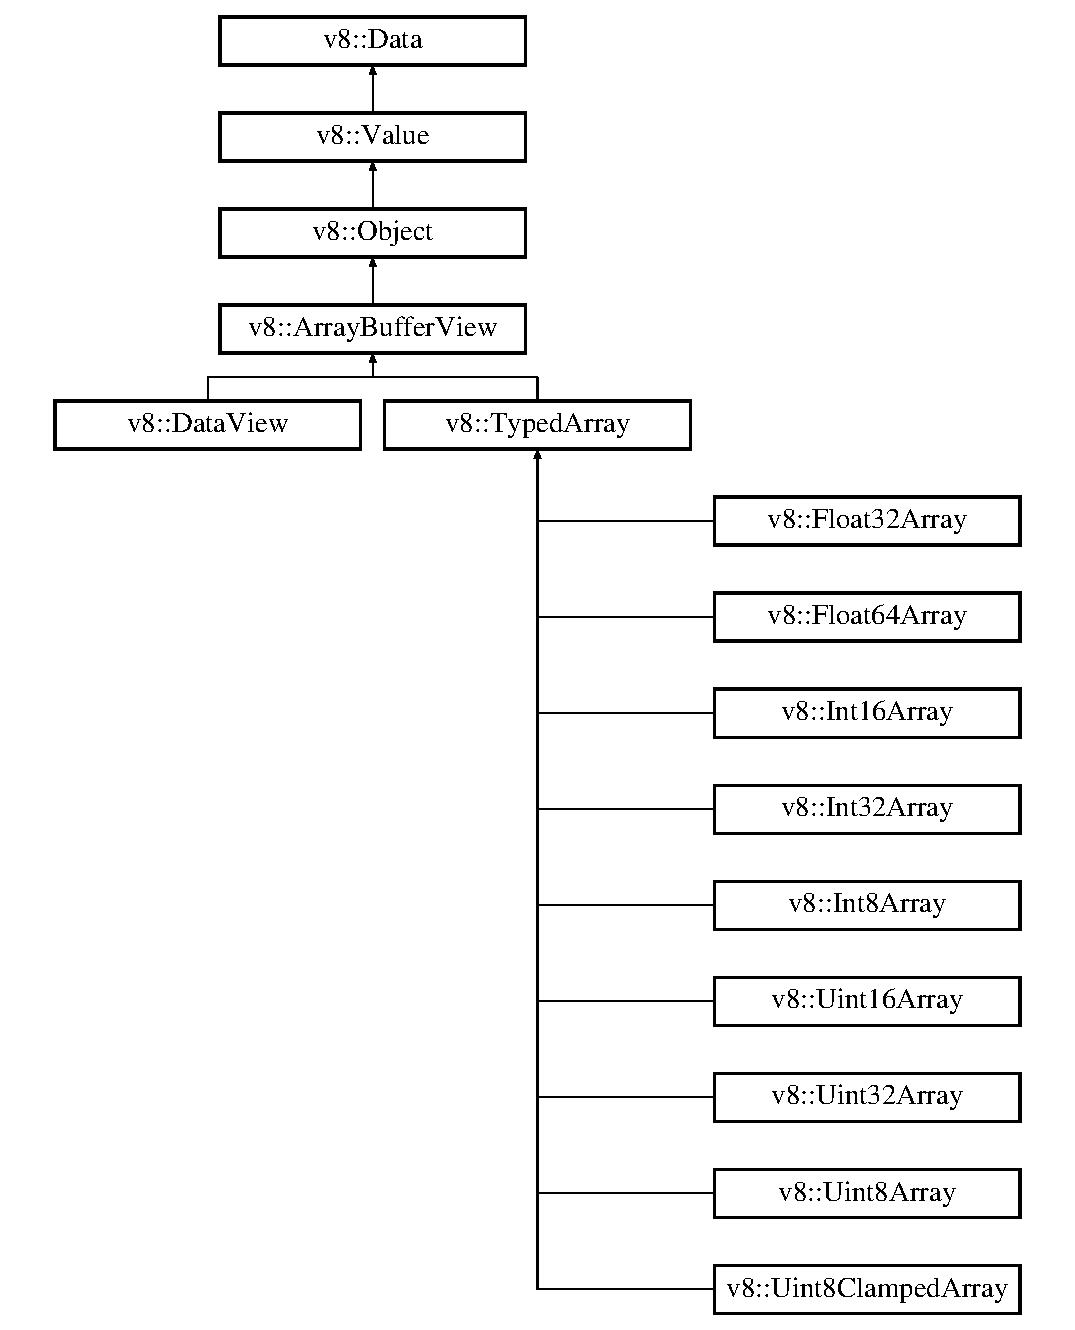
\includegraphics[height=12.000000cm]{classv8_1_1_array_buffer_view}
\end{center}
\end{figure}
\subsection*{Public Member Functions}
\begin{DoxyCompactItemize}
\item 
\hyperlink{classv8_1_1_local}{Local}$<$ \hyperlink{classv8_1_1_array_buffer}{Array\+Buffer} $>$ \hyperlink{classv8_1_1_array_buffer_view_a134c62b37be7a9e8437a56b832f1800a}{Buffer} ()
\item 
size\+\_\+t \hyperlink{classv8_1_1_array_buffer_view_a4739a31269f5ebc5b88a708b9429c688}{Byte\+Offset} ()
\item 
size\+\_\+t \hyperlink{classv8_1_1_array_buffer_view_a9fc7563c97e0b639a6c0a3274995bb3c}{Byte\+Length} ()
\item 
size\+\_\+t \hyperlink{classv8_1_1_array_buffer_view_aa728e762ed43194f3a5e05e792fff64e}{Copy\+Contents} (void $\ast$dest, size\+\_\+t byte\+\_\+length)
\item 
bool \hyperlink{classv8_1_1_array_buffer_view_ab3a7de283cab4140632d190a1e3eef22}{Has\+Buffer} () const 
\end{DoxyCompactItemize}
\subsection*{Static Public Member Functions}
\begin{DoxyCompactItemize}
\item 
static V8\+\_\+\+I\+N\+L\+I\+NE \hyperlink{classv8_1_1_array_buffer_view}{Array\+Buffer\+View} $\ast$ {\bfseries Cast} (\hyperlink{classv8_1_1_value}{Value} $\ast$obj)\hypertarget{classv8_1_1_array_buffer_view_a84db315fe904ca1421c0e8e3f615cccb}{}\label{classv8_1_1_array_buffer_view_a84db315fe904ca1421c0e8e3f615cccb}

\end{DoxyCompactItemize}
\subsection*{Static Public Attributes}
\begin{DoxyCompactItemize}
\item 
static const int {\bfseries k\+Internal\+Field\+Count}
\end{DoxyCompactItemize}
\subsection*{Static Private Member Functions}
\begin{DoxyCompactItemize}
\item 
static void {\bfseries Check\+Cast} (\hyperlink{classv8_1_1_value}{Value} $\ast$obj)\hypertarget{classv8_1_1_array_buffer_view_ab22a11e6d470cebc51942e72f3999722}{}\label{classv8_1_1_array_buffer_view_ab22a11e6d470cebc51942e72f3999722}

\end{DoxyCompactItemize}


\subsection{Detailed Description}
A base class for an instance of one of \char`\"{}views\char`\"{} over \hyperlink{classv8_1_1_array_buffer}{Array\+Buffer}, including Typed\+Arrays and \hyperlink{classv8_1_1_data_view}{Data\+View} (E\+S6 draft 15.\+13).

This A\+PI is experimental and may change significantly. 

\subsection{Member Function Documentation}
\index{v8\+::\+Array\+Buffer\+View@{v8\+::\+Array\+Buffer\+View}!Buffer@{Buffer}}
\index{Buffer@{Buffer}!v8\+::\+Array\+Buffer\+View@{v8\+::\+Array\+Buffer\+View}}
\subsubsection[{\texorpdfstring{Buffer()}{Buffer()}}]{\setlength{\rightskip}{0pt plus 5cm}{\bf Local}$<$ {\bf Array\+Buffer} $>$ v8\+::\+Array\+Buffer\+View\+::\+Buffer (
\begin{DoxyParamCaption}
{}
\end{DoxyParamCaption}
)}\hypertarget{classv8_1_1_array_buffer_view_a134c62b37be7a9e8437a56b832f1800a}{}\label{classv8_1_1_array_buffer_view_a134c62b37be7a9e8437a56b832f1800a}
Returns underlying \hyperlink{classv8_1_1_array_buffer}{Array\+Buffer}. \index{v8\+::\+Array\+Buffer\+View@{v8\+::\+Array\+Buffer\+View}!Byte\+Length@{Byte\+Length}}
\index{Byte\+Length@{Byte\+Length}!v8\+::\+Array\+Buffer\+View@{v8\+::\+Array\+Buffer\+View}}
\subsubsection[{\texorpdfstring{Byte\+Length()}{ByteLength()}}]{\setlength{\rightskip}{0pt plus 5cm}size\+\_\+t v8\+::\+Array\+Buffer\+View\+::\+Byte\+Length (
\begin{DoxyParamCaption}
{}
\end{DoxyParamCaption}
)}\hypertarget{classv8_1_1_array_buffer_view_a9fc7563c97e0b639a6c0a3274995bb3c}{}\label{classv8_1_1_array_buffer_view_a9fc7563c97e0b639a6c0a3274995bb3c}
Size of a view in bytes. \index{v8\+::\+Array\+Buffer\+View@{v8\+::\+Array\+Buffer\+View}!Byte\+Offset@{Byte\+Offset}}
\index{Byte\+Offset@{Byte\+Offset}!v8\+::\+Array\+Buffer\+View@{v8\+::\+Array\+Buffer\+View}}
\subsubsection[{\texorpdfstring{Byte\+Offset()}{ByteOffset()}}]{\setlength{\rightskip}{0pt plus 5cm}size\+\_\+t v8\+::\+Array\+Buffer\+View\+::\+Byte\+Offset (
\begin{DoxyParamCaption}
{}
\end{DoxyParamCaption}
)}\hypertarget{classv8_1_1_array_buffer_view_a4739a31269f5ebc5b88a708b9429c688}{}\label{classv8_1_1_array_buffer_view_a4739a31269f5ebc5b88a708b9429c688}
Byte offset in $\vert$\+Buffer$\vert$. \index{v8\+::\+Array\+Buffer\+View@{v8\+::\+Array\+Buffer\+View}!Copy\+Contents@{Copy\+Contents}}
\index{Copy\+Contents@{Copy\+Contents}!v8\+::\+Array\+Buffer\+View@{v8\+::\+Array\+Buffer\+View}}
\subsubsection[{\texorpdfstring{Copy\+Contents(void $\ast$dest, size\+\_\+t byte\+\_\+length)}{CopyContents(void *dest, size_t byte_length)}}]{\setlength{\rightskip}{0pt plus 5cm}size\+\_\+t v8\+::\+Array\+Buffer\+View\+::\+Copy\+Contents (
\begin{DoxyParamCaption}
\item[{void $\ast$}]{dest, }
\item[{size\+\_\+t}]{byte\+\_\+length}
\end{DoxyParamCaption}
)}\hypertarget{classv8_1_1_array_buffer_view_aa728e762ed43194f3a5e05e792fff64e}{}\label{classv8_1_1_array_buffer_view_aa728e762ed43194f3a5e05e792fff64e}
Copy the contents of the \hyperlink{classv8_1_1_array_buffer_view}{Array\+Buffer\+View}\textquotesingle{}s buffer to an embedder defined memory without additional overhead that calling \hyperlink{classv8_1_1_array_buffer_view_a134c62b37be7a9e8437a56b832f1800a}{Array\+Buffer\+View\+::\+Buffer} might incur.

Will write at most min($\vert$byte\+\_\+length$\vert$, Byte\+Length) bytes starting at Byte\+Offset of the underling buffer to the memory starting at $\vert$dest$\vert$. Returns the number of bytes actually written. \index{v8\+::\+Array\+Buffer\+View@{v8\+::\+Array\+Buffer\+View}!Has\+Buffer@{Has\+Buffer}}
\index{Has\+Buffer@{Has\+Buffer}!v8\+::\+Array\+Buffer\+View@{v8\+::\+Array\+Buffer\+View}}
\subsubsection[{\texorpdfstring{Has\+Buffer() const }{HasBuffer() const }}]{\setlength{\rightskip}{0pt plus 5cm}bool v8\+::\+Array\+Buffer\+View\+::\+Has\+Buffer (
\begin{DoxyParamCaption}
{}
\end{DoxyParamCaption}
) const}\hypertarget{classv8_1_1_array_buffer_view_ab3a7de283cab4140632d190a1e3eef22}{}\label{classv8_1_1_array_buffer_view_ab3a7de283cab4140632d190a1e3eef22}
Returns true if \hyperlink{classv8_1_1_array_buffer_view}{Array\+Buffer\+View}\textquotesingle{}s backing \hyperlink{classv8_1_1_array_buffer}{Array\+Buffer} has already been allocated. 

\subsection{Member Data Documentation}
\index{v8\+::\+Array\+Buffer\+View@{v8\+::\+Array\+Buffer\+View}!k\+Internal\+Field\+Count@{k\+Internal\+Field\+Count}}
\index{k\+Internal\+Field\+Count@{k\+Internal\+Field\+Count}!v8\+::\+Array\+Buffer\+View@{v8\+::\+Array\+Buffer\+View}}
\subsubsection[{\texorpdfstring{k\+Internal\+Field\+Count}{kInternalFieldCount}}]{\setlength{\rightskip}{0pt plus 5cm}const int v8\+::\+Array\+Buffer\+View\+::k\+Internal\+Field\+Count\hspace{0.3cm}{\ttfamily [static]}}\hypertarget{classv8_1_1_array_buffer_view_a1cccb675b1a91e61411fee5918d451db}{}\label{classv8_1_1_array_buffer_view_a1cccb675b1a91e61411fee5918d451db}
{\bfseries Initial value\+:}
\begin{DoxyCode}
=
      V8\_ARRAY\_BUFFER\_VIEW\_INTERNAL\_FIELD\_COUNT
\end{DoxyCode}


The documentation for this class was generated from the following files\+:\begin{DoxyCompactItemize}
\item 
/\+Users/joshgav/node/v8/include/v8.\+h\item 
/\+Users/joshgav/node/v8/src/api.\+cc\end{DoxyCompactItemize}

\hypertarget{classv8_1_1_boolean}{}\section{v8\+:\+:Boolean Class Reference}
\label{classv8_1_1_boolean}\index{v8\+::\+Boolean@{v8\+::\+Boolean}}


{\ttfamily \#include $<$v8.\+h$>$}

Inheritance diagram for v8\+:\+:Boolean\+:\begin{figure}[H]
\begin{center}
\leavevmode
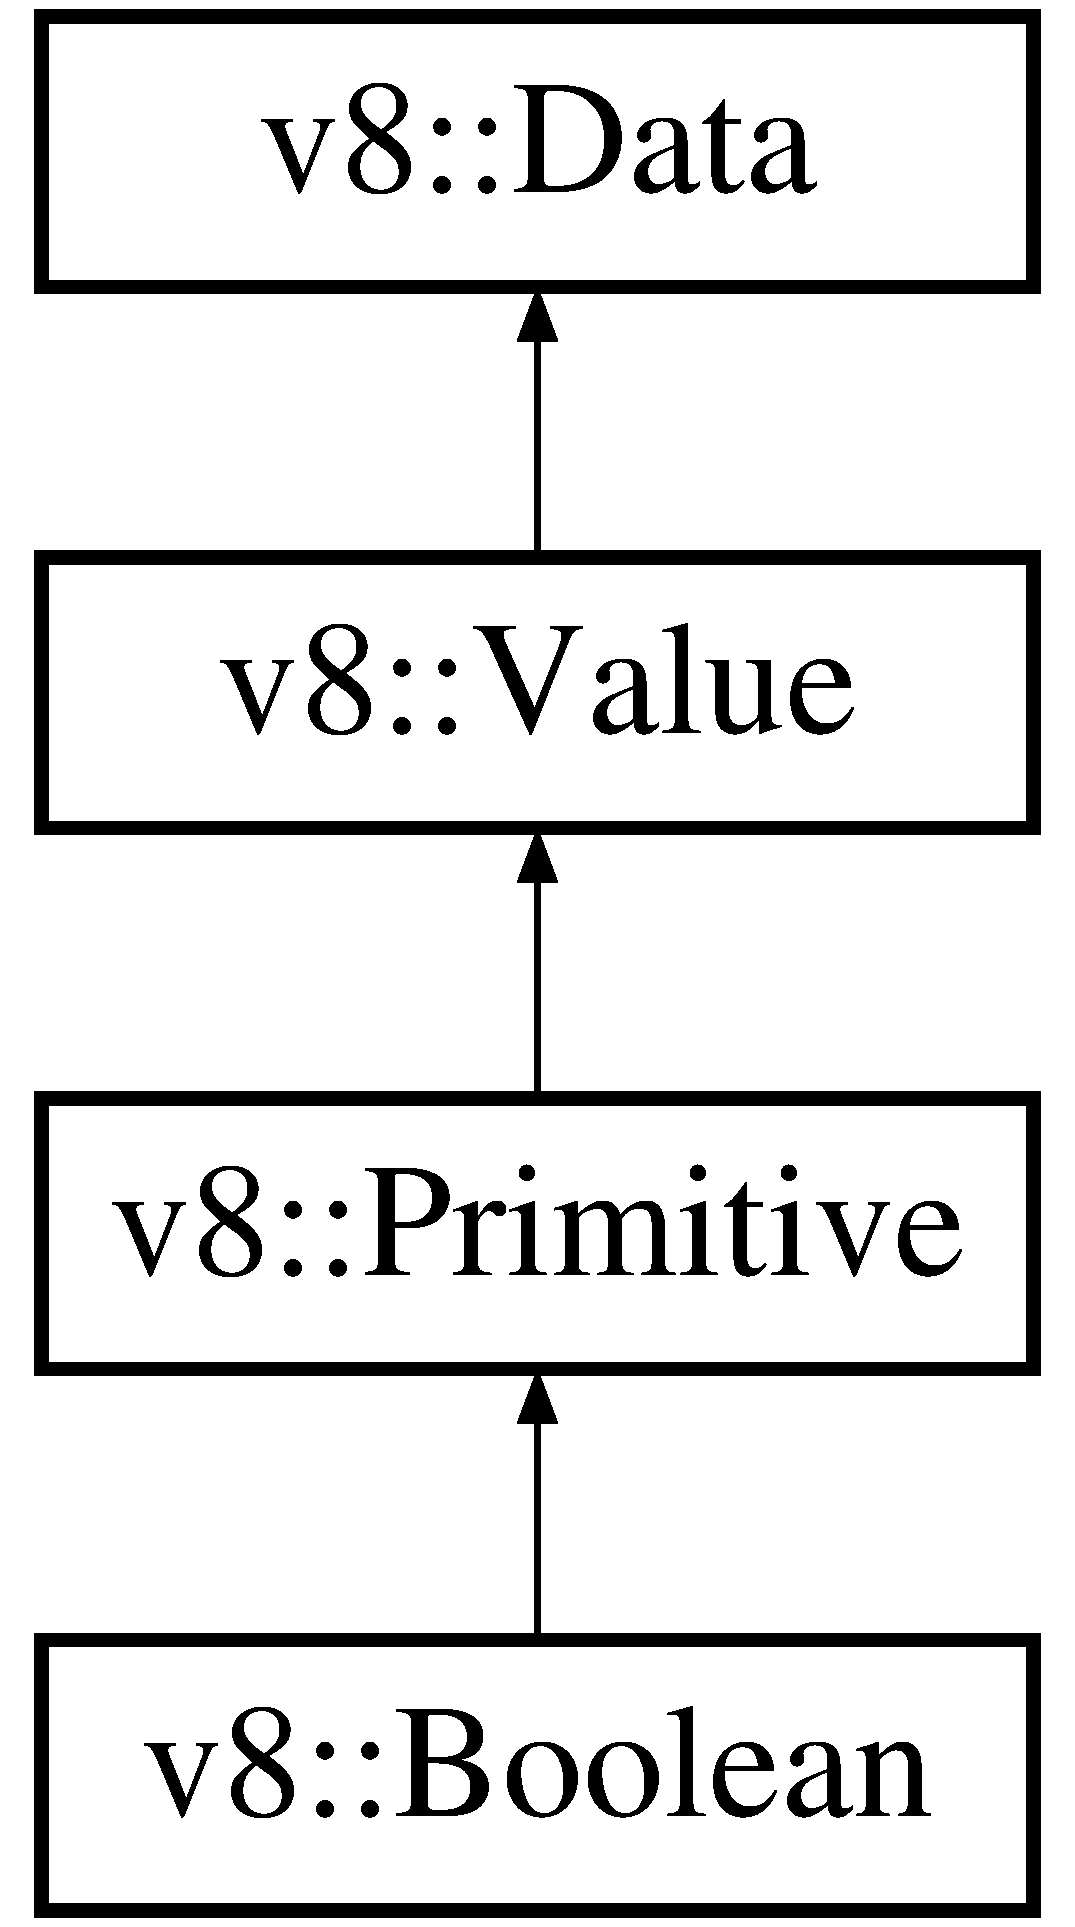
\includegraphics[height=4.000000cm]{classv8_1_1_boolean}
\end{center}
\end{figure}
\subsection*{Public Member Functions}
\begin{DoxyCompactItemize}
\item 
bool {\bfseries Value} () const \hypertarget{classv8_1_1_boolean_aa493d54eb43afc64ab796e1cf66ff910}{}\label{classv8_1_1_boolean_aa493d54eb43afc64ab796e1cf66ff910}

\end{DoxyCompactItemize}
\subsection*{Static Public Member Functions}
\begin{DoxyCompactItemize}
\item 
static V8\+\_\+\+I\+N\+L\+I\+NE \hyperlink{classv8_1_1_boolean}{Boolean} $\ast$ {\bfseries Cast} (\hyperlink{classv8_1_1_value}{v8\+::\+Value} $\ast$obj)\hypertarget{classv8_1_1_boolean_a92493565c4b9400825a0ff09780d7ff4}{}\label{classv8_1_1_boolean_a92493565c4b9400825a0ff09780d7ff4}

\item 
static V8\+\_\+\+I\+N\+L\+I\+NE \hyperlink{classv8_1_1_local}{Local}$<$ \hyperlink{classv8_1_1_boolean}{Boolean} $>$ {\bfseries New} (\hyperlink{classv8_1_1_isolate}{Isolate} $\ast$isolate, bool value)\hypertarget{classv8_1_1_boolean_aeb32aa1bf1853bc4c5f076ee6a8b9a0f}{}\label{classv8_1_1_boolean_aeb32aa1bf1853bc4c5f076ee6a8b9a0f}

\end{DoxyCompactItemize}
\subsection*{Static Private Member Functions}
\begin{DoxyCompactItemize}
\item 
static void {\bfseries Check\+Cast} (\hyperlink{classv8_1_1_value}{v8\+::\+Value} $\ast$obj)\hypertarget{classv8_1_1_boolean_ae8e7c3ba7105247904cb12dfa13d13af}{}\label{classv8_1_1_boolean_ae8e7c3ba7105247904cb12dfa13d13af}

\end{DoxyCompactItemize}


\subsection{Detailed Description}
A primitive boolean value (E\+C\+M\+A-\/262, 4.\+3.\+14). Either the true or false value. 

The documentation for this class was generated from the following file\+:\begin{DoxyCompactItemize}
\item 
include/v8.\+h\end{DoxyCompactItemize}

\hypertarget{classv8_1_1_boolean_object}{}\section{v8\+:\+:Boolean\+Object Class Reference}
\label{classv8_1_1_boolean_object}\index{v8\+::\+Boolean\+Object@{v8\+::\+Boolean\+Object}}


{\ttfamily \#include $<$v8.\+h$>$}

Inheritance diagram for v8\+:\+:Boolean\+Object\+:\begin{figure}[H]
\begin{center}
\leavevmode
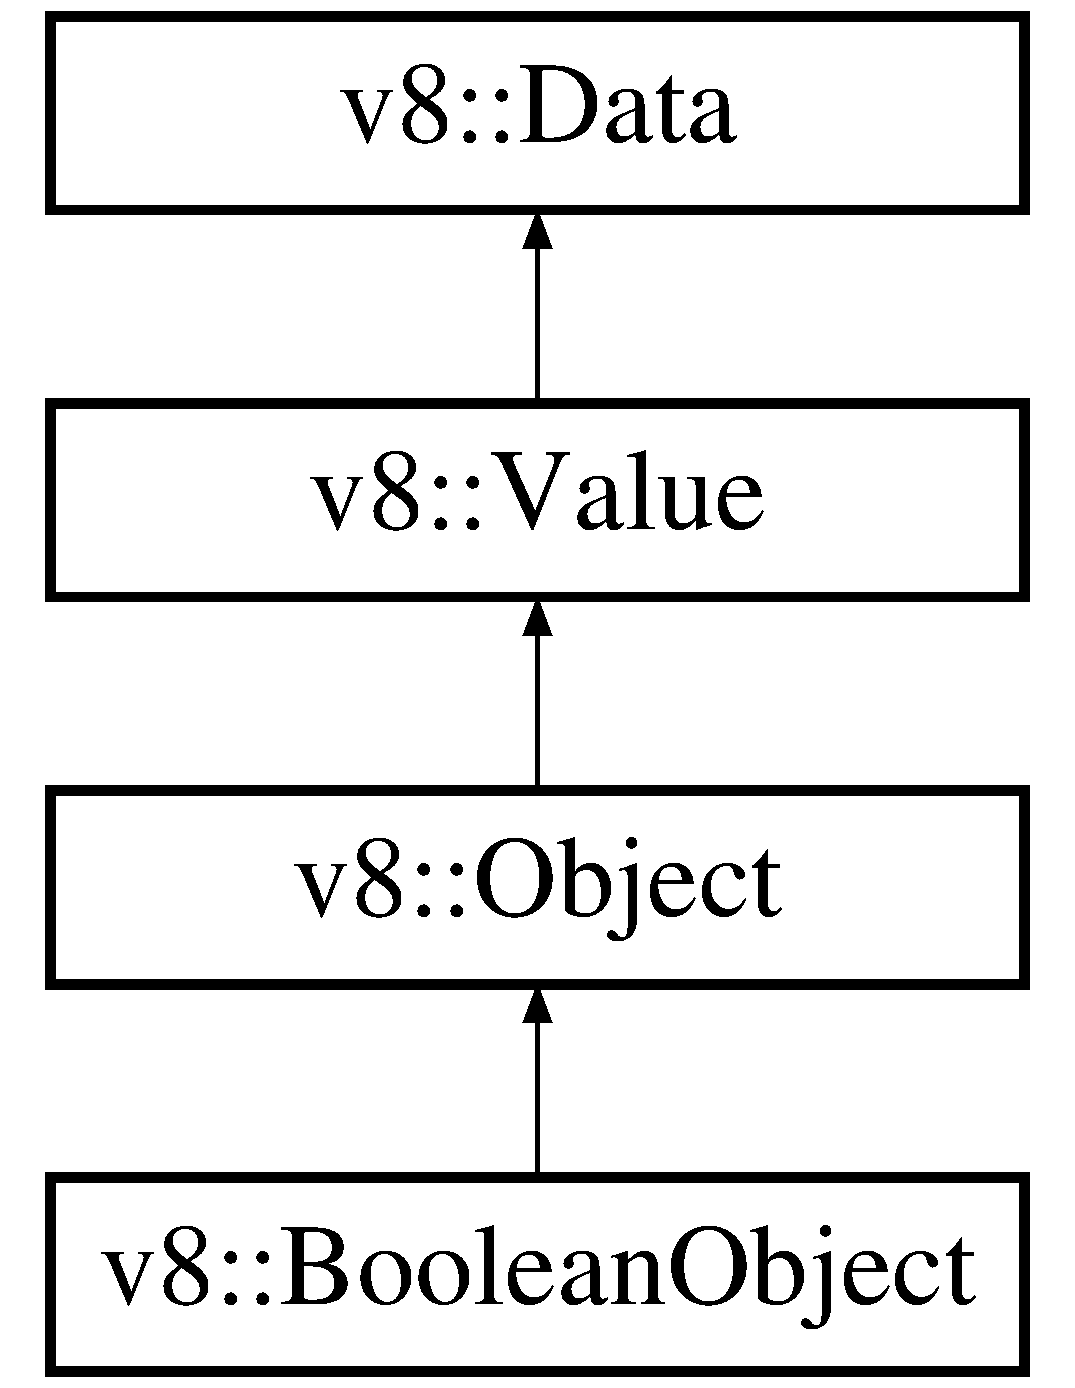
\includegraphics[height=4.000000cm]{classv8_1_1_boolean_object}
\end{center}
\end{figure}
\subsection*{Public Member Functions}
\begin{DoxyCompactItemize}
\item 
{\bfseries V8\+\_\+\+D\+E\+P\+R\+E\+C\+A\+T\+ED} (\char`\"{}Pass an isolate\char`\"{}, static \hyperlink{classv8_1_1_local}{Local}$<$ \hyperlink{classv8_1_1_value}{Value} $>$ New(bool value))\hypertarget{classv8_1_1_boolean_object_ae13a7178a7ee05969b97fa5b0d22cd52}{}\label{classv8_1_1_boolean_object_ae13a7178a7ee05969b97fa5b0d22cd52}

\item 
bool {\bfseries Value\+Of} () const \hypertarget{classv8_1_1_boolean_object_a283419656e641bcd9588dee56c0a0686}{}\label{classv8_1_1_boolean_object_a283419656e641bcd9588dee56c0a0686}

\end{DoxyCompactItemize}
\subsection*{Static Public Member Functions}
\begin{DoxyCompactItemize}
\item 
static \hyperlink{classv8_1_1_local}{Local}$<$ \hyperlink{classv8_1_1_value}{Value} $>$ {\bfseries New} (\hyperlink{classv8_1_1_isolate}{Isolate} $\ast$isolate, bool value)\hypertarget{classv8_1_1_boolean_object_a2cdd408e1318a28cdffe48185f225ec6}{}\label{classv8_1_1_boolean_object_a2cdd408e1318a28cdffe48185f225ec6}

\item 
static V8\+\_\+\+I\+N\+L\+I\+NE \hyperlink{classv8_1_1_boolean_object}{Boolean\+Object} $\ast$ {\bfseries Cast} (\hyperlink{classv8_1_1_value}{v8\+::\+Value} $\ast$obj)\hypertarget{classv8_1_1_boolean_object_ac701398c9b1c74fbce31d66106c9a87f}{}\label{classv8_1_1_boolean_object_ac701398c9b1c74fbce31d66106c9a87f}

\end{DoxyCompactItemize}
\subsection*{Static Private Member Functions}
\begin{DoxyCompactItemize}
\item 
static void {\bfseries Check\+Cast} (\hyperlink{classv8_1_1_value}{v8\+::\+Value} $\ast$obj)\hypertarget{classv8_1_1_boolean_object_a3ef9758674654835f389f2a8cdeb4b4a}{}\label{classv8_1_1_boolean_object_a3ef9758674654835f389f2a8cdeb4b4a}

\end{DoxyCompactItemize}


\subsection{Detailed Description}
A \hyperlink{classv8_1_1_boolean}{Boolean} object (E\+C\+M\+A-\/262, 4.\+3.\+15). 

The documentation for this class was generated from the following files\+:\begin{DoxyCompactItemize}
\item 
/\+Users/joshgav/node/v8/include/v8.\+h\item 
/\+Users/joshgav/node/v8/src/api.\+cc\end{DoxyCompactItemize}

\hypertarget{structv8_1_1_script_compiler_1_1_cached_data}{}\section{v8\+:\+:Script\+Compiler\+:\+:Cached\+Data Struct Reference}
\label{structv8_1_1_script_compiler_1_1_cached_data}\index{v8\+::\+Script\+Compiler\+::\+Cached\+Data@{v8\+::\+Script\+Compiler\+::\+Cached\+Data}}


{\ttfamily \#include $<$v8.\+h$>$}

\subsection*{Public Types}
\begin{DoxyCompactItemize}
\item 
enum {\bfseries Buffer\+Policy} \{ \\*
{\bfseries Buffer\+Not\+Owned}, 
\\*
{\bfseries Buffer\+Owned}
 \}\hypertarget{structv8_1_1_script_compiler_1_1_cached_data_ac1a1055d361e89b589c3fa98b79b9c25}{}\label{structv8_1_1_script_compiler_1_1_cached_data_ac1a1055d361e89b589c3fa98b79b9c25}

\end{DoxyCompactItemize}
\subsection*{Public Member Functions}
\begin{DoxyCompactItemize}
\item 
{\bfseries Cached\+Data} (const uint8\+\_\+t $\ast$data, int length, Buffer\+Policy buffer\+\_\+policy=Buffer\+Not\+Owned)\hypertarget{structv8_1_1_script_compiler_1_1_cached_data_ab45b2bd22aa86eafd0b8eecbdc72d44e}{}\label{structv8_1_1_script_compiler_1_1_cached_data_ab45b2bd22aa86eafd0b8eecbdc72d44e}

\end{DoxyCompactItemize}
\subsection*{Public Attributes}
\begin{DoxyCompactItemize}
\item 
const uint8\+\_\+t $\ast$ {\bfseries data}\hypertarget{structv8_1_1_script_compiler_1_1_cached_data_a31e313a969170116f98d5a76c110fe61}{}\label{structv8_1_1_script_compiler_1_1_cached_data_a31e313a969170116f98d5a76c110fe61}

\item 
int {\bfseries length}\hypertarget{structv8_1_1_script_compiler_1_1_cached_data_ad7b8b1b672095a2c33621d3d5b5c7f8f}{}\label{structv8_1_1_script_compiler_1_1_cached_data_ad7b8b1b672095a2c33621d3d5b5c7f8f}

\item 
bool {\bfseries rejected}\hypertarget{structv8_1_1_script_compiler_1_1_cached_data_aa1d16fbd48957df19d4cc1c886afff8f}{}\label{structv8_1_1_script_compiler_1_1_cached_data_aa1d16fbd48957df19d4cc1c886afff8f}

\item 
Buffer\+Policy {\bfseries buffer\+\_\+policy}\hypertarget{structv8_1_1_script_compiler_1_1_cached_data_a1e5c9ff625ac790139aec4294493fe32}{}\label{structv8_1_1_script_compiler_1_1_cached_data_a1e5c9ff625ac790139aec4294493fe32}

\end{DoxyCompactItemize}
\subsection*{Private Member Functions}
\begin{DoxyCompactItemize}
\item 
{\bfseries Cached\+Data} (const \hyperlink{structv8_1_1_script_compiler_1_1_cached_data}{Cached\+Data} \&)\hypertarget{structv8_1_1_script_compiler_1_1_cached_data_a106962bbaf8753194846eea24f5f952a}{}\label{structv8_1_1_script_compiler_1_1_cached_data_a106962bbaf8753194846eea24f5f952a}

\item 
\hyperlink{structv8_1_1_script_compiler_1_1_cached_data}{Cached\+Data} \& {\bfseries operator=} (const \hyperlink{structv8_1_1_script_compiler_1_1_cached_data}{Cached\+Data} \&)\hypertarget{structv8_1_1_script_compiler_1_1_cached_data_a6f7dcbf54e78b8f0c9bd03321217d84e}{}\label{structv8_1_1_script_compiler_1_1_cached_data_a6f7dcbf54e78b8f0c9bd03321217d84e}

\end{DoxyCompactItemize}


\subsection{Detailed Description}
Compilation data that the embedder can cache and pass back to speed up future compilations. The data is produced if the Compiler\+Options passed to the compilation functions in \hyperlink{classv8_1_1_script_compiler}{Script\+Compiler} contains produce\+\_\+data\+\_\+to\+\_\+cache = true. The data to cache can then can be retrieved from \hyperlink{classv8_1_1_unbound_script}{Unbound\+Script}. 

The documentation for this struct was generated from the following file\+:\begin{DoxyCompactItemize}
\item 
/\+Users/joshgav/node/v8/include/v8.\+h\end{DoxyCompactItemize}

\hypertarget{classv8_1_1_debug_1_1_client_data}{}\section{v8\+:\+:Debug\+:\+:Client\+Data Class Reference}
\label{classv8_1_1_debug_1_1_client_data}\index{v8\+::\+Debug\+::\+Client\+Data@{v8\+::\+Debug\+::\+Client\+Data}}


{\ttfamily \#include $<$v8-\/debug.\+h$>$}



\subsection{Detailed Description}
A client object passed to the \hyperlink{namespacev8}{v8} debugger whose ownership will be taken by it. \hyperlink{namespacev8}{v8} is always responsible for deleting the object. 

The documentation for this class was generated from the following file\+:\begin{DoxyCompactItemize}
\item 
include/v8-\/debug.\+h\end{DoxyCompactItemize}

\hypertarget{classv8_1_1_array_buffer_1_1_contents}{}\section{v8\+:\+:Array\+Buffer\+:\+:Contents Class Reference}
\label{classv8_1_1_array_buffer_1_1_contents}\index{v8\+::\+Array\+Buffer\+::\+Contents@{v8\+::\+Array\+Buffer\+::\+Contents}}


{\ttfamily \#include $<$v8.\+h$>$}

\subsection*{Public Member Functions}
\begin{DoxyCompactItemize}
\item 
void $\ast$ {\bfseries Data} () const \hypertarget{classv8_1_1_array_buffer_1_1_contents_a9ed7556bfaca7a0b24deb05538a76dcd}{}\label{classv8_1_1_array_buffer_1_1_contents_a9ed7556bfaca7a0b24deb05538a76dcd}

\item 
size\+\_\+t {\bfseries Byte\+Length} () const \hypertarget{classv8_1_1_array_buffer_1_1_contents_a1b6a3eecb4fe05f4d33c83b6bc1fa737}{}\label{classv8_1_1_array_buffer_1_1_contents_a1b6a3eecb4fe05f4d33c83b6bc1fa737}

\end{DoxyCompactItemize}
\subsection*{Private Attributes}
\begin{DoxyCompactItemize}
\item 
void $\ast$ {\bfseries data\+\_\+}\hypertarget{classv8_1_1_array_buffer_1_1_contents_adc9777b758068477dd848b7c090ec96d}{}\label{classv8_1_1_array_buffer_1_1_contents_adc9777b758068477dd848b7c090ec96d}

\item 
size\+\_\+t {\bfseries byte\+\_\+length\+\_\+}\hypertarget{classv8_1_1_array_buffer_1_1_contents_afc6781b4a3443c04ea2b17c9c0e9e852}{}\label{classv8_1_1_array_buffer_1_1_contents_afc6781b4a3443c04ea2b17c9c0e9e852}

\end{DoxyCompactItemize}
\subsection*{Friends}
\begin{DoxyCompactItemize}
\item 
class {\bfseries Array\+Buffer}\hypertarget{classv8_1_1_array_buffer_1_1_contents_acbcb25033a90500a51aa19c811b2a1d3}{}\label{classv8_1_1_array_buffer_1_1_contents_acbcb25033a90500a51aa19c811b2a1d3}

\end{DoxyCompactItemize}


\subsection{Detailed Description}
The contents of an $\vert$\+Array\+Buffer$\vert$. Externalization of $\vert$\+Array\+Buffer$\vert$ returns an instance of this class, populated, with a pointer to data and byte length.

The \hyperlink{classv8_1_1_data}{Data} pointer of \hyperlink{classv8_1_1_array_buffer_1_1_contents}{Array\+Buffer\+::\+Contents} is always allocated with \hyperlink{classv8_1_1_array_buffer_1_1_allocator_a106b0d80120ed04fe9b9675e96f0340b}{Allocator\+::\+Allocate} that is set via \hyperlink{structv8_1_1_isolate_1_1_create_params}{Isolate\+::\+Create\+Params}.

This A\+PI is experimental and may change significantly. 

The documentation for this class was generated from the following file\+:\begin{DoxyCompactItemize}
\item 
/\+Users/joshgav/node/v8/include/v8.\+h\end{DoxyCompactItemize}

\hypertarget{classv8_1_1_shared_array_buffer_1_1_contents}{}\section{v8\+:\+:Shared\+Array\+Buffer\+:\+:Contents Class Reference}
\label{classv8_1_1_shared_array_buffer_1_1_contents}\index{v8\+::\+Shared\+Array\+Buffer\+::\+Contents@{v8\+::\+Shared\+Array\+Buffer\+::\+Contents}}


{\ttfamily \#include $<$v8.\+h$>$}

\subsection*{Public Member Functions}
\begin{DoxyCompactItemize}
\item 
void $\ast$ {\bfseries Data} () const \hypertarget{classv8_1_1_shared_array_buffer_1_1_contents_a7e25a8f041d968fb7af4c4ae72dd2dc7}{}\label{classv8_1_1_shared_array_buffer_1_1_contents_a7e25a8f041d968fb7af4c4ae72dd2dc7}

\item 
size\+\_\+t {\bfseries Byte\+Length} () const \hypertarget{classv8_1_1_shared_array_buffer_1_1_contents_a68fb3080f3304278ec47c2cfddfec0ae}{}\label{classv8_1_1_shared_array_buffer_1_1_contents_a68fb3080f3304278ec47c2cfddfec0ae}

\end{DoxyCompactItemize}
\subsection*{Private Attributes}
\begin{DoxyCompactItemize}
\item 
void $\ast$ {\bfseries data\+\_\+}\hypertarget{classv8_1_1_shared_array_buffer_1_1_contents_a28e46bb2a558606f7b6bde08cf98c5b3}{}\label{classv8_1_1_shared_array_buffer_1_1_contents_a28e46bb2a558606f7b6bde08cf98c5b3}

\item 
size\+\_\+t {\bfseries byte\+\_\+length\+\_\+}\hypertarget{classv8_1_1_shared_array_buffer_1_1_contents_a270e00df31c57697fe250a8535e67f43}{}\label{classv8_1_1_shared_array_buffer_1_1_contents_a270e00df31c57697fe250a8535e67f43}

\end{DoxyCompactItemize}
\subsection*{Friends}
\begin{DoxyCompactItemize}
\item 
class {\bfseries Shared\+Array\+Buffer}\hypertarget{classv8_1_1_shared_array_buffer_1_1_contents_a35ac2a80dda42f728b7b1dfc4c3cc040}{}\label{classv8_1_1_shared_array_buffer_1_1_contents_a35ac2a80dda42f728b7b1dfc4c3cc040}

\end{DoxyCompactItemize}


\subsection{Detailed Description}
The contents of an $\vert$\+Shared\+Array\+Buffer$\vert$. Externalization of $\vert$\+Shared\+Array\+Buffer$\vert$ returns an instance of this class, populated, with a pointer to data and byte length.

The \hyperlink{classv8_1_1_data}{Data} pointer of \hyperlink{classv8_1_1_shared_array_buffer_1_1_contents}{Shared\+Array\+Buffer\+::\+Contents} is always allocated with $\vert$\+Array\+Buffer\+::\+Allocator\+::\+Allocate$\vert$ by the allocator specified in \hyperlink{structv8_1_1_isolate_1_1_create_params_a7c663f70b64290392eeaf164f57585f9}{v8\+::\+Isolate\+::\+Create\+Params\+::array\+\_\+buffer\+\_\+allocator}.

This A\+PI is experimental and may change significantly. 

The documentation for this class was generated from the following file\+:\begin{DoxyCompactItemize}
\item 
include/v8.\+h\end{DoxyCompactItemize}

\hypertarget{classv8_1_1_context}{}\section{v8\+:\+:Context Class Reference}
\label{classv8_1_1_context}\index{v8\+::\+Context@{v8\+::\+Context}}


{\ttfamily \#include $<$v8.\+h$>$}

\subsection*{Classes}
\begin{DoxyCompactItemize}
\item 
class \hyperlink{classv8_1_1_context_1_1_scope}{Scope}
\end{DoxyCompactItemize}
\subsection*{Public Types}
\begin{DoxyCompactItemize}
\item 
enum \hyperlink{classv8_1_1_context_a8e8a8c567e2d193f25f1ec211db0b5f9}{Embedder\+Data\+Fields} \{ {\bfseries k\+Debug\+Id\+Index} = 0
 \}
\end{DoxyCompactItemize}
\subsection*{Public Member Functions}
\begin{DoxyCompactItemize}
\item 
\hyperlink{classv8_1_1_local}{Local}$<$ \hyperlink{classv8_1_1_object}{Object} $>$ \hyperlink{classv8_1_1_context_af5cd9f97ef6a3307c1c21f80f4b743eb}{Global} ()
\item 
void \hyperlink{classv8_1_1_context_a841c7dd92eb8c57df92a268a164dea97}{Detach\+Global} ()
\item 
void \hyperlink{classv8_1_1_context_a2351d9bdf4450d5f23734033289ba3ab}{Set\+Security\+Token} (\hyperlink{classv8_1_1_local}{Local}$<$ \hyperlink{classv8_1_1_value}{Value} $>$ token)
\item 
void \hyperlink{classv8_1_1_context_aa9e1a14982b64fd51ab87600a287bad2}{Use\+Default\+Security\+Token} ()
\item 
\hyperlink{classv8_1_1_local}{Local}$<$ \hyperlink{classv8_1_1_value}{Value} $>$ \hyperlink{classv8_1_1_context_a59d7bc98684603ec4d9b1d1db2acaad8}{Get\+Security\+Token} ()
\item 
void \hyperlink{classv8_1_1_context_a6995c49d9897eb49053f07874b825133}{Enter} ()
\item 
void \hyperlink{classv8_1_1_context_a2db09d4fefb26023a40d88972a4c1599}{Exit} ()
\item 
\hyperlink{classv8_1_1_isolate}{v8\+::\+Isolate} $\ast$ \hyperlink{classv8_1_1_context_af55552d8658ecb20eff7af2c83e8ede2}{Get\+Isolate} ()
\item 
V8\+\_\+\+I\+N\+L\+I\+NE \hyperlink{classv8_1_1_local}{Local}$<$ \hyperlink{classv8_1_1_value}{Value} $>$ \hyperlink{classv8_1_1_context_a9cfafe0ac56f6aee17eb80a913489296}{Get\+Embedder\+Data} (int index)
\item 
\hyperlink{classv8_1_1_local}{Local}$<$ \hyperlink{classv8_1_1_object}{Object} $>$ \hyperlink{classv8_1_1_context_aa06026c0a9dc43874b437675b8fd0059}{Get\+Extras\+Binding\+Object} ()
\item 
void \hyperlink{classv8_1_1_context_a1f2f3da0b9c3d9b68a5384b757d607d2}{Set\+Embedder\+Data} (int index, \hyperlink{classv8_1_1_local}{Local}$<$ \hyperlink{classv8_1_1_value}{Value} $>$ value)
\item 
V8\+\_\+\+I\+N\+L\+I\+NE void $\ast$ \hyperlink{classv8_1_1_context_aa3b5c1a1a5d145c6096840898013f559}{Get\+Aligned\+Pointer\+From\+Embedder\+Data} (int index)
\item 
void \hyperlink{classv8_1_1_context_a522063c88e4c2832f5ff4f3980815f58}{Set\+Aligned\+Pointer\+In\+Embedder\+Data} (int index, void $\ast$value)
\item 
void \hyperlink{classv8_1_1_context_a794ccc42113566f5d363f89c8b0d3c2c}{Allow\+Code\+Generation\+From\+Strings} (bool allow)
\item 
bool \hyperlink{classv8_1_1_context_aa7a960a232d232d1a2a904c2e6c18831}{Is\+Code\+Generation\+From\+Strings\+Allowed} ()
\item 
void \hyperlink{classv8_1_1_context_a8c919ccddb6fbb65602f7fe2587e8a34}{Set\+Error\+Message\+For\+Code\+Generation\+From\+Strings} (\hyperlink{classv8_1_1_local}{Local}$<$ \hyperlink{classv8_1_1_string}{String} $>$ message)
\item 
size\+\_\+t \hyperlink{classv8_1_1_context_abfec90cb6cb1cac58b4e3487515721a2}{Estimated\+Size} ()
\end{DoxyCompactItemize}
\subsection*{Static Public Member Functions}
\begin{DoxyCompactItemize}
\item 
static \hyperlink{classv8_1_1_local}{Local}$<$ \hyperlink{classv8_1_1_context}{Context} $>$ \hyperlink{classv8_1_1_context_aee22d1422b0804b5b6bc0646bfd29af8}{New} (\hyperlink{classv8_1_1_isolate}{Isolate} $\ast$isolate, \hyperlink{classv8_1_1_extension_configuration}{Extension\+Configuration} $\ast$extensions=N\+U\+LL, \hyperlink{classv8_1_1_local}{Local}$<$ \hyperlink{classv8_1_1_object_template}{Object\+Template} $>$ global\+\_\+template=\hyperlink{classv8_1_1_local}{Local}$<$ \hyperlink{classv8_1_1_object_template}{Object\+Template} $>$(), \hyperlink{classv8_1_1_local}{Local}$<$ \hyperlink{classv8_1_1_value}{Value} $>$ global\+\_\+object=\hyperlink{classv8_1_1_local}{Local}$<$ \hyperlink{classv8_1_1_value}{Value} $>$())
\end{DoxyCompactItemize}
\subsection*{Private Member Functions}
\begin{DoxyCompactItemize}
\item 
\hyperlink{classv8_1_1_local}{Local}$<$ \hyperlink{classv8_1_1_value}{Value} $>$ {\bfseries Slow\+Get\+Embedder\+Data} (int index)\hypertarget{classv8_1_1_context_a5c27c14fa755c7430e54ae864e329011}{}\label{classv8_1_1_context_a5c27c14fa755c7430e54ae864e329011}

\item 
void $\ast$ {\bfseries Slow\+Get\+Aligned\+Pointer\+From\+Embedder\+Data} (int index)\hypertarget{classv8_1_1_context_ae79782ecf2b811fa20ceb735059842d5}{}\label{classv8_1_1_context_ae79782ecf2b811fa20ceb735059842d5}

\end{DoxyCompactItemize}
\subsection*{Friends}
\begin{DoxyCompactItemize}
\item 
class {\bfseries Value}\hypertarget{classv8_1_1_context_aeceedf6e1a7d48a588516ce2b1983d6f}{}\label{classv8_1_1_context_aeceedf6e1a7d48a588516ce2b1983d6f}

\item 
class {\bfseries Script}\hypertarget{classv8_1_1_context_ae98eaa96d1b24e087f3c3e372fb09dce}{}\label{classv8_1_1_context_ae98eaa96d1b24e087f3c3e372fb09dce}

\item 
class {\bfseries Object}\hypertarget{classv8_1_1_context_a0720b5f434e636e22a3ed34f847eec57}{}\label{classv8_1_1_context_a0720b5f434e636e22a3ed34f847eec57}

\item 
class {\bfseries Function}\hypertarget{classv8_1_1_context_ab7194606aa12931e96f8f5448d418ed0}{}\label{classv8_1_1_context_ab7194606aa12931e96f8f5448d418ed0}

\end{DoxyCompactItemize}


\subsection{Detailed Description}
A sandboxed execution context with its own set of built-\/in objects and functions. 

\subsection{Member Enumeration Documentation}
\index{v8\+::\+Context@{v8\+::\+Context}!Embedder\+Data\+Fields@{Embedder\+Data\+Fields}}
\index{Embedder\+Data\+Fields@{Embedder\+Data\+Fields}!v8\+::\+Context@{v8\+::\+Context}}
\subsubsection[{\texorpdfstring{Embedder\+Data\+Fields}{EmbedderDataFields}}]{\setlength{\rightskip}{0pt plus 5cm}enum {\bf v8\+::\+Context\+::\+Embedder\+Data\+Fields}}\hypertarget{classv8_1_1_context_a8e8a8c567e2d193f25f1ec211db0b5f9}{}\label{classv8_1_1_context_a8e8a8c567e2d193f25f1ec211db0b5f9}
The field at k\+Debug\+Id\+Index is reserved for \hyperlink{classv8_1_1_v8}{V8} debugger implementation. The value is propagated to the scripts compiled in given \hyperlink{classv8_1_1_context}{Context} and can be used for filtering scripts. 

\subsection{Member Function Documentation}
\index{v8\+::\+Context@{v8\+::\+Context}!Allow\+Code\+Generation\+From\+Strings@{Allow\+Code\+Generation\+From\+Strings}}
\index{Allow\+Code\+Generation\+From\+Strings@{Allow\+Code\+Generation\+From\+Strings}!v8\+::\+Context@{v8\+::\+Context}}
\subsubsection[{\texorpdfstring{Allow\+Code\+Generation\+From\+Strings(bool allow)}{AllowCodeGenerationFromStrings(bool allow)}}]{\setlength{\rightskip}{0pt plus 5cm}void v8\+::\+Context\+::\+Allow\+Code\+Generation\+From\+Strings (
\begin{DoxyParamCaption}
\item[{bool}]{allow}
\end{DoxyParamCaption}
)}\hypertarget{classv8_1_1_context_a794ccc42113566f5d363f89c8b0d3c2c}{}\label{classv8_1_1_context_a794ccc42113566f5d363f89c8b0d3c2c}
Control whether code generation from strings is allowed. Calling this method with false will disable \textquotesingle{}eval\textquotesingle{} and the \textquotesingle{}\hyperlink{classv8_1_1_function}{Function}\textquotesingle{} constructor for code running in this context. If \textquotesingle{}eval\textquotesingle{} or the \textquotesingle{}\hyperlink{classv8_1_1_function}{Function}\textquotesingle{} constructor are used an exception will be thrown.

If code generation from strings is not allowed the V8\+::\+Allow\+Code\+Generation\+From\+Strings callback will be invoked if set before blocking the call to \textquotesingle{}eval\textquotesingle{} or the \textquotesingle{}\hyperlink{classv8_1_1_function}{Function}\textquotesingle{} constructor. If that callback returns true, the call will be allowed, otherwise an exception will be thrown. If no callback is set an exception will be thrown. \index{v8\+::\+Context@{v8\+::\+Context}!Detach\+Global@{Detach\+Global}}
\index{Detach\+Global@{Detach\+Global}!v8\+::\+Context@{v8\+::\+Context}}
\subsubsection[{\texorpdfstring{Detach\+Global()}{DetachGlobal()}}]{\setlength{\rightskip}{0pt plus 5cm}void v8\+::\+Context\+::\+Detach\+Global (
\begin{DoxyParamCaption}
{}
\end{DoxyParamCaption}
)}\hypertarget{classv8_1_1_context_a841c7dd92eb8c57df92a268a164dea97}{}\label{classv8_1_1_context_a841c7dd92eb8c57df92a268a164dea97}
Detaches the global object from its context before the global object can be reused to create a new context. \index{v8\+::\+Context@{v8\+::\+Context}!Enter@{Enter}}
\index{Enter@{Enter}!v8\+::\+Context@{v8\+::\+Context}}
\subsubsection[{\texorpdfstring{Enter()}{Enter()}}]{\setlength{\rightskip}{0pt plus 5cm}void v8\+::\+Context\+::\+Enter (
\begin{DoxyParamCaption}
{}
\end{DoxyParamCaption}
)}\hypertarget{classv8_1_1_context_a6995c49d9897eb49053f07874b825133}{}\label{classv8_1_1_context_a6995c49d9897eb49053f07874b825133}
Enter this context. After entering a context, all code compiled and run is compiled and run in this context. If another context is already entered, this old context is saved so it can be restored when the new context is exited. \index{v8\+::\+Context@{v8\+::\+Context}!Estimated\+Size@{Estimated\+Size}}
\index{Estimated\+Size@{Estimated\+Size}!v8\+::\+Context@{v8\+::\+Context}}
\subsubsection[{\texorpdfstring{Estimated\+Size()}{EstimatedSize()}}]{\setlength{\rightskip}{0pt plus 5cm}size\+\_\+t v8\+::\+Context\+::\+Estimated\+Size (
\begin{DoxyParamCaption}
{}
\end{DoxyParamCaption}
)}\hypertarget{classv8_1_1_context_abfec90cb6cb1cac58b4e3487515721a2}{}\label{classv8_1_1_context_abfec90cb6cb1cac58b4e3487515721a2}
Estimate the memory in bytes retained by this context. \index{v8\+::\+Context@{v8\+::\+Context}!Exit@{Exit}}
\index{Exit@{Exit}!v8\+::\+Context@{v8\+::\+Context}}
\subsubsection[{\texorpdfstring{Exit()}{Exit()}}]{\setlength{\rightskip}{0pt plus 5cm}void v8\+::\+Context\+::\+Exit (
\begin{DoxyParamCaption}
{}
\end{DoxyParamCaption}
)}\hypertarget{classv8_1_1_context_a2db09d4fefb26023a40d88972a4c1599}{}\label{classv8_1_1_context_a2db09d4fefb26023a40d88972a4c1599}
Exit this context. Exiting the current context restores the context that was in place when entering the current context. \index{v8\+::\+Context@{v8\+::\+Context}!Get\+Aligned\+Pointer\+From\+Embedder\+Data@{Get\+Aligned\+Pointer\+From\+Embedder\+Data}}
\index{Get\+Aligned\+Pointer\+From\+Embedder\+Data@{Get\+Aligned\+Pointer\+From\+Embedder\+Data}!v8\+::\+Context@{v8\+::\+Context}}
\subsubsection[{\texorpdfstring{Get\+Aligned\+Pointer\+From\+Embedder\+Data(int index)}{GetAlignedPointerFromEmbedderData(int index)}}]{\setlength{\rightskip}{0pt plus 5cm}void $\ast$ v8\+::\+Context\+::\+Get\+Aligned\+Pointer\+From\+Embedder\+Data (
\begin{DoxyParamCaption}
\item[{int}]{index}
\end{DoxyParamCaption}
)}\hypertarget{classv8_1_1_context_aa3b5c1a1a5d145c6096840898013f559}{}\label{classv8_1_1_context_aa3b5c1a1a5d145c6096840898013f559}
Gets a 2-\/byte-\/aligned native pointer from the embedder data with the given index, which must have bees set by a previous call to Set\+Aligned\+Pointer\+In\+Embedder\+Data with the same index. Note that index 0 currently has a special meaning for Chrome\textquotesingle{}s debugger. \index{v8\+::\+Context@{v8\+::\+Context}!Get\+Embedder\+Data@{Get\+Embedder\+Data}}
\index{Get\+Embedder\+Data@{Get\+Embedder\+Data}!v8\+::\+Context@{v8\+::\+Context}}
\subsubsection[{\texorpdfstring{Get\+Embedder\+Data(int index)}{GetEmbedderData(int index)}}]{\setlength{\rightskip}{0pt plus 5cm}{\bf Local}$<$ {\bf Value} $>$ v8\+::\+Context\+::\+Get\+Embedder\+Data (
\begin{DoxyParamCaption}
\item[{int}]{index}
\end{DoxyParamCaption}
)}\hypertarget{classv8_1_1_context_a9cfafe0ac56f6aee17eb80a913489296}{}\label{classv8_1_1_context_a9cfafe0ac56f6aee17eb80a913489296}
Gets the embedder data with the given index, which must have been set by a previous call to Set\+Embedder\+Data with the same index. Note that index 0 currently has a special meaning for Chrome\textquotesingle{}s debugger. \index{v8\+::\+Context@{v8\+::\+Context}!Get\+Extras\+Binding\+Object@{Get\+Extras\+Binding\+Object}}
\index{Get\+Extras\+Binding\+Object@{Get\+Extras\+Binding\+Object}!v8\+::\+Context@{v8\+::\+Context}}
\subsubsection[{\texorpdfstring{Get\+Extras\+Binding\+Object()}{GetExtrasBindingObject()}}]{\setlength{\rightskip}{0pt plus 5cm}{\bf Local}$<${\bf Object}$>$ v8\+::\+Context\+::\+Get\+Extras\+Binding\+Object (
\begin{DoxyParamCaption}
{}
\end{DoxyParamCaption}
)}\hypertarget{classv8_1_1_context_aa06026c0a9dc43874b437675b8fd0059}{}\label{classv8_1_1_context_aa06026c0a9dc43874b437675b8fd0059}
Gets the binding object used by \hyperlink{classv8_1_1_v8}{V8} extras. Extra natives get a reference to this object and can use it to \char`\"{}export\char`\"{} functionality by adding properties. Extra natives can also \char`\"{}import\char`\"{} functionality by accessing properties added by the embedder using the \hyperlink{classv8_1_1_v8}{V8} A\+PI. \index{v8\+::\+Context@{v8\+::\+Context}!Get\+Isolate@{Get\+Isolate}}
\index{Get\+Isolate@{Get\+Isolate}!v8\+::\+Context@{v8\+::\+Context}}
\subsubsection[{\texorpdfstring{Get\+Isolate()}{GetIsolate()}}]{\setlength{\rightskip}{0pt plus 5cm}{\bf v8\+::\+Isolate}$\ast$ v8\+::\+Context\+::\+Get\+Isolate (
\begin{DoxyParamCaption}
{}
\end{DoxyParamCaption}
)}\hypertarget{classv8_1_1_context_af55552d8658ecb20eff7af2c83e8ede2}{}\label{classv8_1_1_context_af55552d8658ecb20eff7af2c83e8ede2}
Returns an isolate associated with a current context. \index{v8\+::\+Context@{v8\+::\+Context}!Get\+Security\+Token@{Get\+Security\+Token}}
\index{Get\+Security\+Token@{Get\+Security\+Token}!v8\+::\+Context@{v8\+::\+Context}}
\subsubsection[{\texorpdfstring{Get\+Security\+Token()}{GetSecurityToken()}}]{\setlength{\rightskip}{0pt plus 5cm}{\bf Local}$<${\bf Value}$>$ v8\+::\+Context\+::\+Get\+Security\+Token (
\begin{DoxyParamCaption}
{}
\end{DoxyParamCaption}
)}\hypertarget{classv8_1_1_context_a59d7bc98684603ec4d9b1d1db2acaad8}{}\label{classv8_1_1_context_a59d7bc98684603ec4d9b1d1db2acaad8}
Returns the security token of this context. \index{v8\+::\+Context@{v8\+::\+Context}!Global@{Global}}
\index{Global@{Global}!v8\+::\+Context@{v8\+::\+Context}}
\subsubsection[{\texorpdfstring{Global()}{Global()}}]{\setlength{\rightskip}{0pt plus 5cm}{\bf Local}$<${\bf Object}$>$ v8\+::\+Context\+::\+Global (
\begin{DoxyParamCaption}
{}
\end{DoxyParamCaption}
)}\hypertarget{classv8_1_1_context_af5cd9f97ef6a3307c1c21f80f4b743eb}{}\label{classv8_1_1_context_af5cd9f97ef6a3307c1c21f80f4b743eb}
Returns the global proxy object.

\hyperlink{classv8_1_1_global}{Global} proxy object is a thin wrapper whose prototype points to actual context\textquotesingle{}s global object with the properties like \hyperlink{classv8_1_1_object}{Object}, etc. This is done that way for security reasons (for more details see \href{https://wiki.mozilla.org/Gecko:SplitWindow}{\tt https\+://wiki.\+mozilla.\+org/\+Gecko\+:\+Split\+Window}).

Please note that changes to global proxy object prototype most probably would break VM---\hyperlink{namespacev8}{v8} expects only global object as a prototype of global proxy object. \index{v8\+::\+Context@{v8\+::\+Context}!Is\+Code\+Generation\+From\+Strings\+Allowed@{Is\+Code\+Generation\+From\+Strings\+Allowed}}
\index{Is\+Code\+Generation\+From\+Strings\+Allowed@{Is\+Code\+Generation\+From\+Strings\+Allowed}!v8\+::\+Context@{v8\+::\+Context}}
\subsubsection[{\texorpdfstring{Is\+Code\+Generation\+From\+Strings\+Allowed()}{IsCodeGenerationFromStringsAllowed()}}]{\setlength{\rightskip}{0pt plus 5cm}bool v8\+::\+Context\+::\+Is\+Code\+Generation\+From\+Strings\+Allowed (
\begin{DoxyParamCaption}
{}
\end{DoxyParamCaption}
)}\hypertarget{classv8_1_1_context_aa7a960a232d232d1a2a904c2e6c18831}{}\label{classv8_1_1_context_aa7a960a232d232d1a2a904c2e6c18831}
Returns true if code generation from strings is allowed for the context. For more details see \hyperlink{classv8_1_1_context_a794ccc42113566f5d363f89c8b0d3c2c}{Allow\+Code\+Generation\+From\+Strings(bool)} documentation. \index{v8\+::\+Context@{v8\+::\+Context}!New@{New}}
\index{New@{New}!v8\+::\+Context@{v8\+::\+Context}}
\subsubsection[{\texorpdfstring{New(\+Isolate $\ast$isolate, Extension\+Configuration $\ast$extensions=\+N\+U\+L\+L, Local$<$ Object\+Template $>$ global\+\_\+template=\+Local$<$ Object\+Template $>$(), Local$<$ Value $>$ global\+\_\+object=\+Local$<$ Value $>$())}{New(Isolate *isolate, ExtensionConfiguration *extensions=NULL, Local< ObjectTemplate > global_template=Local< ObjectTemplate >(), Local< Value > global_object=Local< Value >())}}]{\setlength{\rightskip}{0pt plus 5cm}static {\bf Local}$<${\bf Context}$>$ v8\+::\+Context\+::\+New (
\begin{DoxyParamCaption}
\item[{{\bf Isolate} $\ast$}]{isolate, }
\item[{{\bf Extension\+Configuration} $\ast$}]{extensions = {\ttfamily NULL}, }
\item[{{\bf Local}$<$ {\bf Object\+Template} $>$}]{global\+\_\+template = {\ttfamily {\bf Local}$<$~{\bf Object\+Template}~$>$()}, }
\item[{{\bf Local}$<$ {\bf Value} $>$}]{global\+\_\+object = {\ttfamily {\bf Local}$<$~{\bf Value}~$>$()}}
\end{DoxyParamCaption}
)\hspace{0.3cm}{\ttfamily [static]}}\hypertarget{classv8_1_1_context_aee22d1422b0804b5b6bc0646bfd29af8}{}\label{classv8_1_1_context_aee22d1422b0804b5b6bc0646bfd29af8}
Creates a new context and returns a handle to the newly allocated context.


\begin{DoxyParams}{Parameters}
{\em isolate} & The isolate in which to create the context.\\
\hline
{\em extensions} & An optional extension configuration containing the extensions to be installed in the newly created context.\\
\hline
{\em global\+\_\+template} & An optional object template from which the global object for the newly created context will be created.\\
\hline
{\em global\+\_\+object} & An optional global object to be reused for the newly created context. This global object must have been created by a previous call to \hyperlink{classv8_1_1_context_aee22d1422b0804b5b6bc0646bfd29af8}{Context\+::\+New} with the same global template. The state of the global object will be completely reset and only object identify will remain. \\
\hline
\end{DoxyParams}
\index{v8\+::\+Context@{v8\+::\+Context}!Set\+Aligned\+Pointer\+In\+Embedder\+Data@{Set\+Aligned\+Pointer\+In\+Embedder\+Data}}
\index{Set\+Aligned\+Pointer\+In\+Embedder\+Data@{Set\+Aligned\+Pointer\+In\+Embedder\+Data}!v8\+::\+Context@{v8\+::\+Context}}
\subsubsection[{\texorpdfstring{Set\+Aligned\+Pointer\+In\+Embedder\+Data(int index, void $\ast$value)}{SetAlignedPointerInEmbedderData(int index, void *value)}}]{\setlength{\rightskip}{0pt plus 5cm}void v8\+::\+Context\+::\+Set\+Aligned\+Pointer\+In\+Embedder\+Data (
\begin{DoxyParamCaption}
\item[{int}]{index, }
\item[{void $\ast$}]{value}
\end{DoxyParamCaption}
)}\hypertarget{classv8_1_1_context_a522063c88e4c2832f5ff4f3980815f58}{}\label{classv8_1_1_context_a522063c88e4c2832f5ff4f3980815f58}
Sets a 2-\/byte-\/aligned native pointer in the embedder data with the given index, growing the data as needed. Note that index 0 currently has a special meaning for Chrome\textquotesingle{}s debugger. \index{v8\+::\+Context@{v8\+::\+Context}!Set\+Embedder\+Data@{Set\+Embedder\+Data}}
\index{Set\+Embedder\+Data@{Set\+Embedder\+Data}!v8\+::\+Context@{v8\+::\+Context}}
\subsubsection[{\texorpdfstring{Set\+Embedder\+Data(int index, Local$<$ Value $>$ value)}{SetEmbedderData(int index, Local< Value > value)}}]{\setlength{\rightskip}{0pt plus 5cm}void v8\+::\+Context\+::\+Set\+Embedder\+Data (
\begin{DoxyParamCaption}
\item[{int}]{index, }
\item[{{\bf Local}$<$ {\bf Value} $>$}]{value}
\end{DoxyParamCaption}
)}\hypertarget{classv8_1_1_context_a1f2f3da0b9c3d9b68a5384b757d607d2}{}\label{classv8_1_1_context_a1f2f3da0b9c3d9b68a5384b757d607d2}
Sets the embedder data with the given index, growing the data as needed. Note that index 0 currently has a special meaning for Chrome\textquotesingle{}s debugger. \index{v8\+::\+Context@{v8\+::\+Context}!Set\+Error\+Message\+For\+Code\+Generation\+From\+Strings@{Set\+Error\+Message\+For\+Code\+Generation\+From\+Strings}}
\index{Set\+Error\+Message\+For\+Code\+Generation\+From\+Strings@{Set\+Error\+Message\+For\+Code\+Generation\+From\+Strings}!v8\+::\+Context@{v8\+::\+Context}}
\subsubsection[{\texorpdfstring{Set\+Error\+Message\+For\+Code\+Generation\+From\+Strings(\+Local$<$ String $>$ message)}{SetErrorMessageForCodeGenerationFromStrings(Local< String > message)}}]{\setlength{\rightskip}{0pt plus 5cm}void v8\+::\+Context\+::\+Set\+Error\+Message\+For\+Code\+Generation\+From\+Strings (
\begin{DoxyParamCaption}
\item[{{\bf Local}$<$ {\bf String} $>$}]{message}
\end{DoxyParamCaption}
)}\hypertarget{classv8_1_1_context_a8c919ccddb6fbb65602f7fe2587e8a34}{}\label{classv8_1_1_context_a8c919ccddb6fbb65602f7fe2587e8a34}
Sets the error description for the exception that is thrown when code generation from strings is not allowed and \textquotesingle{}eval\textquotesingle{} or the \textquotesingle{}\hyperlink{classv8_1_1_function}{Function}\textquotesingle{} constructor are called. \index{v8\+::\+Context@{v8\+::\+Context}!Set\+Security\+Token@{Set\+Security\+Token}}
\index{Set\+Security\+Token@{Set\+Security\+Token}!v8\+::\+Context@{v8\+::\+Context}}
\subsubsection[{\texorpdfstring{Set\+Security\+Token(\+Local$<$ Value $>$ token)}{SetSecurityToken(Local< Value > token)}}]{\setlength{\rightskip}{0pt plus 5cm}void v8\+::\+Context\+::\+Set\+Security\+Token (
\begin{DoxyParamCaption}
\item[{{\bf Local}$<$ {\bf Value} $>$}]{token}
\end{DoxyParamCaption}
)}\hypertarget{classv8_1_1_context_a2351d9bdf4450d5f23734033289ba3ab}{}\label{classv8_1_1_context_a2351d9bdf4450d5f23734033289ba3ab}
Sets the security token for the context. To access an object in another context, the security tokens must match. \index{v8\+::\+Context@{v8\+::\+Context}!Use\+Default\+Security\+Token@{Use\+Default\+Security\+Token}}
\index{Use\+Default\+Security\+Token@{Use\+Default\+Security\+Token}!v8\+::\+Context@{v8\+::\+Context}}
\subsubsection[{\texorpdfstring{Use\+Default\+Security\+Token()}{UseDefaultSecurityToken()}}]{\setlength{\rightskip}{0pt plus 5cm}void v8\+::\+Context\+::\+Use\+Default\+Security\+Token (
\begin{DoxyParamCaption}
{}
\end{DoxyParamCaption}
)}\hypertarget{classv8_1_1_context_aa9e1a14982b64fd51ab87600a287bad2}{}\label{classv8_1_1_context_aa9e1a14982b64fd51ab87600a287bad2}
Restores the security token to the default value. 

The documentation for this class was generated from the following file\+:\begin{DoxyCompactItemize}
\item 
include/v8.\+h\end{DoxyCompactItemize}

\hypertarget{structv8_1_1_copyable_persistent_traits}{}\section{v8\+:\+:Copyable\+Persistent\+Traits$<$ T $>$ Struct Template Reference}
\label{structv8_1_1_copyable_persistent_traits}\index{v8\+::\+Copyable\+Persistent\+Traits$<$ T $>$@{v8\+::\+Copyable\+Persistent\+Traits$<$ T $>$}}


{\ttfamily \#include $<$v8.\+h$>$}

\subsection*{Public Types}
\begin{DoxyCompactItemize}
\item 
typedef \hyperlink{classv8_1_1_persistent}{Persistent}$<$ T, \hyperlink{structv8_1_1_copyable_persistent_traits}{Copyable\+Persistent\+Traits}$<$ T $>$ $>$ {\bfseries Copyable\+Persistent}\hypertarget{structv8_1_1_copyable_persistent_traits_a327724a22ee06da5ae54dd29982d068e}{}\label{structv8_1_1_copyable_persistent_traits_a327724a22ee06da5ae54dd29982d068e}

\end{DoxyCompactItemize}
\subsection*{Static Public Member Functions}
\begin{DoxyCompactItemize}
\item 
{\footnotesize template$<$class S , class M $>$ }\\static V8\+\_\+\+I\+N\+L\+I\+NE void {\bfseries Copy} (const \hyperlink{classv8_1_1_persistent}{Persistent}$<$ S, M $>$ \&source, \hyperlink{classv8_1_1_persistent}{Copyable\+Persistent} $\ast$dest)\hypertarget{structv8_1_1_copyable_persistent_traits_aa8adf12936633b5f13b624541acaa1cf}{}\label{structv8_1_1_copyable_persistent_traits_aa8adf12936633b5f13b624541acaa1cf}

\end{DoxyCompactItemize}
\subsection*{Static Public Attributes}
\begin{DoxyCompactItemize}
\item 
static const bool {\bfseries k\+Reset\+In\+Destructor} = true\hypertarget{structv8_1_1_copyable_persistent_traits_a1a10842e15d8ee11f78da030bdffd025}{}\label{structv8_1_1_copyable_persistent_traits_a1a10842e15d8ee11f78da030bdffd025}

\end{DoxyCompactItemize}


\subsection{Detailed Description}
\subsubsection*{template$<$class T$>$\\*
struct v8\+::\+Copyable\+Persistent\+Traits$<$ T $>$}

Helper class traits to allow copying and assignment of \hyperlink{classv8_1_1_persistent}{Persistent}. This will clone the contents of storage cell, but not any of the flags, etc. 

The documentation for this struct was generated from the following file\+:\begin{DoxyCompactItemize}
\item 
/\+Users/joshgav/node/v8/include/v8.\+h\end{DoxyCompactItemize}

\hypertarget{classv8_1_1_cpu_profile}{}\section{v8\+:\+:Cpu\+Profile Class Reference}
\label{classv8_1_1_cpu_profile}\index{v8\+::\+Cpu\+Profile@{v8\+::\+Cpu\+Profile}}


{\ttfamily \#include $<$v8-\/profiler.\+h$>$}

\subsection*{Public Member Functions}
\begin{DoxyCompactItemize}
\item 
\hyperlink{classv8_1_1_local}{Local}$<$ \hyperlink{classv8_1_1_string}{String} $>$ \hyperlink{classv8_1_1_cpu_profile_a34cc58f44862c27ea781ce47ca79f74e}{Get\+Title} () const 
\item 
const \hyperlink{classv8_1_1_cpu_profile_node}{Cpu\+Profile\+Node} $\ast$ \hyperlink{classv8_1_1_cpu_profile_aec978f073af6634b6495baa65209a31f}{Get\+Top\+Down\+Root} () const 
\item 
int \hyperlink{classv8_1_1_cpu_profile_a2ca9d8e862dc2b06892196b5e5a14994}{Get\+Samples\+Count} () const 
\item 
const \hyperlink{classv8_1_1_cpu_profile_node}{Cpu\+Profile\+Node} $\ast$ \hyperlink{classv8_1_1_cpu_profile_a59470cd1286e949dd069eea87777a074}{Get\+Sample} (int index) const 
\item 
int64\+\_\+t \hyperlink{classv8_1_1_cpu_profile_a310b49cf2ac856821b5db5dd856580e7}{Get\+Sample\+Timestamp} (int index) const 
\item 
int64\+\_\+t \hyperlink{classv8_1_1_cpu_profile_aac317de54bdfc4523b5ecea522c01ad1}{Get\+Start\+Time} () const 
\item 
int64\+\_\+t \hyperlink{classv8_1_1_cpu_profile_a15170e2e9eeb972fddf949bd08dd09ff}{Get\+End\+Time} () const 
\item 
void \hyperlink{classv8_1_1_cpu_profile_a70c93f0c14d07a7e1bad42ee95665ca0}{Delete} ()
\end{DoxyCompactItemize}


\subsection{Detailed Description}
\hyperlink{classv8_1_1_cpu_profile}{Cpu\+Profile} contains a C\+PU profile in a form of top-\/down call tree (from main() down to functions that do all the work). 

\subsection{Member Function Documentation}
\index{v8\+::\+Cpu\+Profile@{v8\+::\+Cpu\+Profile}!Delete@{Delete}}
\index{Delete@{Delete}!v8\+::\+Cpu\+Profile@{v8\+::\+Cpu\+Profile}}
\subsubsection[{\texorpdfstring{Delete()}{Delete()}}]{\setlength{\rightskip}{0pt plus 5cm}void v8\+::\+Cpu\+Profile\+::\+Delete (
\begin{DoxyParamCaption}
{}
\end{DoxyParamCaption}
)}\hypertarget{classv8_1_1_cpu_profile_a70c93f0c14d07a7e1bad42ee95665ca0}{}\label{classv8_1_1_cpu_profile_a70c93f0c14d07a7e1bad42ee95665ca0}
Deletes the profile and removes it from \hyperlink{classv8_1_1_cpu_profiler}{Cpu\+Profiler}\textquotesingle{}s list. All pointers to nodes previously returned become invalid. \index{v8\+::\+Cpu\+Profile@{v8\+::\+Cpu\+Profile}!Get\+End\+Time@{Get\+End\+Time}}
\index{Get\+End\+Time@{Get\+End\+Time}!v8\+::\+Cpu\+Profile@{v8\+::\+Cpu\+Profile}}
\subsubsection[{\texorpdfstring{Get\+End\+Time() const }{GetEndTime() const }}]{\setlength{\rightskip}{0pt plus 5cm}int64\+\_\+t v8\+::\+Cpu\+Profile\+::\+Get\+End\+Time (
\begin{DoxyParamCaption}
{}
\end{DoxyParamCaption}
) const}\hypertarget{classv8_1_1_cpu_profile_a15170e2e9eeb972fddf949bd08dd09ff}{}\label{classv8_1_1_cpu_profile_a15170e2e9eeb972fddf949bd08dd09ff}
Returns time when the profile recording was stopped (in microseconds) since some unspecified starting point. The point is equal to the starting point used by Get\+Start\+Time. \index{v8\+::\+Cpu\+Profile@{v8\+::\+Cpu\+Profile}!Get\+Sample@{Get\+Sample}}
\index{Get\+Sample@{Get\+Sample}!v8\+::\+Cpu\+Profile@{v8\+::\+Cpu\+Profile}}
\subsubsection[{\texorpdfstring{Get\+Sample(int index) const }{GetSample(int index) const }}]{\setlength{\rightskip}{0pt plus 5cm}const {\bf Cpu\+Profile\+Node}$\ast$ v8\+::\+Cpu\+Profile\+::\+Get\+Sample (
\begin{DoxyParamCaption}
\item[{int}]{index}
\end{DoxyParamCaption}
) const}\hypertarget{classv8_1_1_cpu_profile_a59470cd1286e949dd069eea87777a074}{}\label{classv8_1_1_cpu_profile_a59470cd1286e949dd069eea87777a074}
Returns profile node corresponding to the top frame the sample at the given index. \index{v8\+::\+Cpu\+Profile@{v8\+::\+Cpu\+Profile}!Get\+Samples\+Count@{Get\+Samples\+Count}}
\index{Get\+Samples\+Count@{Get\+Samples\+Count}!v8\+::\+Cpu\+Profile@{v8\+::\+Cpu\+Profile}}
\subsubsection[{\texorpdfstring{Get\+Samples\+Count() const }{GetSamplesCount() const }}]{\setlength{\rightskip}{0pt plus 5cm}int v8\+::\+Cpu\+Profile\+::\+Get\+Samples\+Count (
\begin{DoxyParamCaption}
{}
\end{DoxyParamCaption}
) const}\hypertarget{classv8_1_1_cpu_profile_a2ca9d8e862dc2b06892196b5e5a14994}{}\label{classv8_1_1_cpu_profile_a2ca9d8e862dc2b06892196b5e5a14994}
Returns number of samples recorded. The samples are not recorded unless $\vert$record\+\_\+samples$\vert$ parameter of Cpu\+Profiler\+::\+Start\+Cpu\+Profiling is true. \index{v8\+::\+Cpu\+Profile@{v8\+::\+Cpu\+Profile}!Get\+Sample\+Timestamp@{Get\+Sample\+Timestamp}}
\index{Get\+Sample\+Timestamp@{Get\+Sample\+Timestamp}!v8\+::\+Cpu\+Profile@{v8\+::\+Cpu\+Profile}}
\subsubsection[{\texorpdfstring{Get\+Sample\+Timestamp(int index) const }{GetSampleTimestamp(int index) const }}]{\setlength{\rightskip}{0pt plus 5cm}int64\+\_\+t v8\+::\+Cpu\+Profile\+::\+Get\+Sample\+Timestamp (
\begin{DoxyParamCaption}
\item[{int}]{index}
\end{DoxyParamCaption}
) const}\hypertarget{classv8_1_1_cpu_profile_a310b49cf2ac856821b5db5dd856580e7}{}\label{classv8_1_1_cpu_profile_a310b49cf2ac856821b5db5dd856580e7}
Returns the timestamp of the sample. The timestamp is the number of microseconds since some unspecified starting point. The point is equal to the starting point used by Get\+Start\+Time. \index{v8\+::\+Cpu\+Profile@{v8\+::\+Cpu\+Profile}!Get\+Start\+Time@{Get\+Start\+Time}}
\index{Get\+Start\+Time@{Get\+Start\+Time}!v8\+::\+Cpu\+Profile@{v8\+::\+Cpu\+Profile}}
\subsubsection[{\texorpdfstring{Get\+Start\+Time() const }{GetStartTime() const }}]{\setlength{\rightskip}{0pt plus 5cm}int64\+\_\+t v8\+::\+Cpu\+Profile\+::\+Get\+Start\+Time (
\begin{DoxyParamCaption}
{}
\end{DoxyParamCaption}
) const}\hypertarget{classv8_1_1_cpu_profile_aac317de54bdfc4523b5ecea522c01ad1}{}\label{classv8_1_1_cpu_profile_aac317de54bdfc4523b5ecea522c01ad1}
Returns time when the profile recording was started (in microseconds) since some unspecified starting point. \index{v8\+::\+Cpu\+Profile@{v8\+::\+Cpu\+Profile}!Get\+Title@{Get\+Title}}
\index{Get\+Title@{Get\+Title}!v8\+::\+Cpu\+Profile@{v8\+::\+Cpu\+Profile}}
\subsubsection[{\texorpdfstring{Get\+Title() const }{GetTitle() const }}]{\setlength{\rightskip}{0pt plus 5cm}{\bf Local}$<${\bf String}$>$ v8\+::\+Cpu\+Profile\+::\+Get\+Title (
\begin{DoxyParamCaption}
{}
\end{DoxyParamCaption}
) const}\hypertarget{classv8_1_1_cpu_profile_a34cc58f44862c27ea781ce47ca79f74e}{}\label{classv8_1_1_cpu_profile_a34cc58f44862c27ea781ce47ca79f74e}
Returns C\+PU profile title. \index{v8\+::\+Cpu\+Profile@{v8\+::\+Cpu\+Profile}!Get\+Top\+Down\+Root@{Get\+Top\+Down\+Root}}
\index{Get\+Top\+Down\+Root@{Get\+Top\+Down\+Root}!v8\+::\+Cpu\+Profile@{v8\+::\+Cpu\+Profile}}
\subsubsection[{\texorpdfstring{Get\+Top\+Down\+Root() const }{GetTopDownRoot() const }}]{\setlength{\rightskip}{0pt plus 5cm}const {\bf Cpu\+Profile\+Node}$\ast$ v8\+::\+Cpu\+Profile\+::\+Get\+Top\+Down\+Root (
\begin{DoxyParamCaption}
{}
\end{DoxyParamCaption}
) const}\hypertarget{classv8_1_1_cpu_profile_aec978f073af6634b6495baa65209a31f}{}\label{classv8_1_1_cpu_profile_aec978f073af6634b6495baa65209a31f}
Returns the root node of the top down call tree. 

The documentation for this class was generated from the following file\+:\begin{DoxyCompactItemize}
\item 
include/v8-\/profiler.\+h\end{DoxyCompactItemize}

\hypertarget{structv8_1_1_cpu_profile_deopt_frame}{}\section{v8\+:\+:Cpu\+Profile\+Deopt\+Frame Struct Reference}
\label{structv8_1_1_cpu_profile_deopt_frame}\index{v8\+::\+Cpu\+Profile\+Deopt\+Frame@{v8\+::\+Cpu\+Profile\+Deopt\+Frame}}
\subsection*{Public Attributes}
\begin{DoxyCompactItemize}
\item 
int {\bfseries script\+\_\+id}\hypertarget{structv8_1_1_cpu_profile_deopt_frame_af7b750288458a70a81b4c05869b8f6d7}{}\label{structv8_1_1_cpu_profile_deopt_frame_af7b750288458a70a81b4c05869b8f6d7}

\item 
size\+\_\+t {\bfseries position}\hypertarget{structv8_1_1_cpu_profile_deopt_frame_a4f82d1517fd15573bb2890961496a76f}{}\label{structv8_1_1_cpu_profile_deopt_frame_a4f82d1517fd15573bb2890961496a76f}

\end{DoxyCompactItemize}


The documentation for this struct was generated from the following file\+:\begin{DoxyCompactItemize}
\item 
/\+Users/joshgav/node/v8/include/v8-\/profiler.\+h\end{DoxyCompactItemize}

\hypertarget{structv8_1_1_cpu_profile_deopt_info}{}\section{v8\+:\+:Cpu\+Profile\+Deopt\+Info Struct Reference}
\label{structv8_1_1_cpu_profile_deopt_info}\index{v8\+::\+Cpu\+Profile\+Deopt\+Info@{v8\+::\+Cpu\+Profile\+Deopt\+Info}}
\subsection*{Public Attributes}
\begin{DoxyCompactItemize}
\item 
const char $\ast$ \hyperlink{structv8_1_1_cpu_profile_deopt_info_a908eb3ba33b47ace8973eeb2fda96ca9}{deopt\+\_\+reason}
\item 
std\+::vector$<$ \hyperlink{structv8_1_1_cpu_profile_deopt_frame}{Cpu\+Profile\+Deopt\+Frame} $>$ {\bfseries stack}\hypertarget{structv8_1_1_cpu_profile_deopt_info_a9446493c0e0a00e3ada02ba8df858d42}{}\label{structv8_1_1_cpu_profile_deopt_info_a9446493c0e0a00e3ada02ba8df858d42}

\end{DoxyCompactItemize}


\subsection{Member Data Documentation}
\index{v8\+::\+Cpu\+Profile\+Deopt\+Info@{v8\+::\+Cpu\+Profile\+Deopt\+Info}!deopt\+\_\+reason@{deopt\+\_\+reason}}
\index{deopt\+\_\+reason@{deopt\+\_\+reason}!v8\+::\+Cpu\+Profile\+Deopt\+Info@{v8\+::\+Cpu\+Profile\+Deopt\+Info}}
\subsubsection[{\texorpdfstring{deopt\+\_\+reason}{deopt_reason}}]{\setlength{\rightskip}{0pt plus 5cm}const char$\ast$ v8\+::\+Cpu\+Profile\+Deopt\+Info\+::deopt\+\_\+reason}\hypertarget{structv8_1_1_cpu_profile_deopt_info_a908eb3ba33b47ace8973eeb2fda96ca9}{}\label{structv8_1_1_cpu_profile_deopt_info_a908eb3ba33b47ace8973eeb2fda96ca9}
A pointer to a static string owned by \hyperlink{namespacev8}{v8}. 

The documentation for this struct was generated from the following file\+:\begin{DoxyCompactItemize}
\item 
include/v8-\/profiler.\+h\end{DoxyCompactItemize}

\hypertarget{classv8_1_1_cpu_profile_node}{}\section{v8\+:\+:Cpu\+Profile\+Node Class Reference}
\label{classv8_1_1_cpu_profile_node}\index{v8\+::\+Cpu\+Profile\+Node@{v8\+::\+Cpu\+Profile\+Node}}


{\ttfamily \#include $<$v8-\/profiler.\+h$>$}

\subsection*{Classes}
\begin{DoxyCompactItemize}
\item 
struct \hyperlink{structv8_1_1_cpu_profile_node_1_1_line_tick}{Line\+Tick}
\end{DoxyCompactItemize}
\subsection*{Public Member Functions}
\begin{DoxyCompactItemize}
\item 
\hyperlink{classv8_1_1_local}{Local}$<$ \hyperlink{classv8_1_1_string}{String} $>$ \hyperlink{classv8_1_1_cpu_profile_node_ab8fab0fb0d118d872155a2862a908b7b}{Get\+Function\+Name} () const 
\item 
int \hyperlink{classv8_1_1_cpu_profile_node_acf6f384df08ec40ff306d3e229f77258}{Get\+Script\+Id} () const 
\item 
\hyperlink{classv8_1_1_local}{Local}$<$ \hyperlink{classv8_1_1_string}{String} $>$ \hyperlink{classv8_1_1_cpu_profile_node_a1b279762d459d331148f7374c699e98b}{Get\+Script\+Resource\+Name} () const 
\item 
int \hyperlink{classv8_1_1_cpu_profile_node_a45ea035661c7152e4f3eb47f73787a75}{Get\+Line\+Number} () const 
\item 
int \hyperlink{classv8_1_1_cpu_profile_node_a43cf237ea6f254a61a6e2a81d554aa1a}{Get\+Column\+Number} () const 
\item 
unsigned int \hyperlink{classv8_1_1_cpu_profile_node_ac0d6015d3859e29db07f6a7e574426d3}{Get\+Hit\+Line\+Count} () const 
\item 
bool \hyperlink{classv8_1_1_cpu_profile_node_af31611e24f47519e82b52b49969ed0a4}{Get\+Line\+Ticks} (\hyperlink{structv8_1_1_cpu_profile_node_1_1_line_tick}{Line\+Tick} $\ast$entries, unsigned int length) const 
\item 
const char $\ast$ \hyperlink{classv8_1_1_cpu_profile_node_afd7aa4d59f97effc345b644b48651f35}{Get\+Bailout\+Reason} () const 
\item 
unsigned \hyperlink{classv8_1_1_cpu_profile_node_a8d297f185b0bbd9f6853f6ed193b656e}{Get\+Hit\+Count} () const 
\item 
unsigned \hyperlink{classv8_1_1_cpu_profile_node_a245092eb223b948fc9441664d9e2701e}{Get\+Call\+Uid} () const 
\item 
unsigned \hyperlink{classv8_1_1_cpu_profile_node_ae2971c5003353a984ef72b6cddf5e298}{Get\+Node\+Id} () const 
\item 
int \hyperlink{classv8_1_1_cpu_profile_node_ac4612b91e43a2901ac20c3705288955b}{Get\+Children\+Count} () const 
\item 
const \hyperlink{classv8_1_1_cpu_profile_node}{Cpu\+Profile\+Node} $\ast$ \hyperlink{classv8_1_1_cpu_profile_node_a52a3bc18d11ebb6c59ccc72caf44c9c3}{Get\+Child} (int index) const 
\item 
const std\+::vector$<$ \hyperlink{structv8_1_1_cpu_profile_deopt_info}{Cpu\+Profile\+Deopt\+Info} $>$ \& \hyperlink{classv8_1_1_cpu_profile_node_a94ec354401e320ccacf95055d3b7577f}{Get\+Deopt\+Infos} () const 
\end{DoxyCompactItemize}
\subsection*{Static Public Attributes}
\begin{DoxyCompactItemize}
\item 
static const int {\bfseries k\+No\+Line\+Number\+Info} = Message\+::k\+No\+Line\+Number\+Info\hypertarget{classv8_1_1_cpu_profile_node_ad54213fe8a795cb6669566f0272fc5ba}{}\label{classv8_1_1_cpu_profile_node_ad54213fe8a795cb6669566f0272fc5ba}

\item 
static const int {\bfseries k\+No\+Column\+Number\+Info} = Message\+::k\+No\+Column\+Info\hypertarget{classv8_1_1_cpu_profile_node_a7c8c1dea3ae0cf4c219b7b1f15a8405b}{}\label{classv8_1_1_cpu_profile_node_a7c8c1dea3ae0cf4c219b7b1f15a8405b}

\end{DoxyCompactItemize}


\subsection{Detailed Description}
\hyperlink{classv8_1_1_cpu_profile_node}{Cpu\+Profile\+Node} represents a node in a call graph. 

\subsection{Member Function Documentation}
\index{v8\+::\+Cpu\+Profile\+Node@{v8\+::\+Cpu\+Profile\+Node}!Get\+Bailout\+Reason@{Get\+Bailout\+Reason}}
\index{Get\+Bailout\+Reason@{Get\+Bailout\+Reason}!v8\+::\+Cpu\+Profile\+Node@{v8\+::\+Cpu\+Profile\+Node}}
\subsubsection[{\texorpdfstring{Get\+Bailout\+Reason() const }{GetBailoutReason() const }}]{\setlength{\rightskip}{0pt plus 5cm}const char $\ast$ v8\+::\+Cpu\+Profile\+Node\+::\+Get\+Bailout\+Reason (
\begin{DoxyParamCaption}
{}
\end{DoxyParamCaption}
) const}\hypertarget{classv8_1_1_cpu_profile_node_afd7aa4d59f97effc345b644b48651f35}{}\label{classv8_1_1_cpu_profile_node_afd7aa4d59f97effc345b644b48651f35}
Returns bailout reason for the function if the optimization was disabled for it. \index{v8\+::\+Cpu\+Profile\+Node@{v8\+::\+Cpu\+Profile\+Node}!Get\+Call\+Uid@{Get\+Call\+Uid}}
\index{Get\+Call\+Uid@{Get\+Call\+Uid}!v8\+::\+Cpu\+Profile\+Node@{v8\+::\+Cpu\+Profile\+Node}}
\subsubsection[{\texorpdfstring{Get\+Call\+Uid() const }{GetCallUid() const }}]{\setlength{\rightskip}{0pt plus 5cm}unsigned v8\+::\+Cpu\+Profile\+Node\+::\+Get\+Call\+Uid (
\begin{DoxyParamCaption}
{}
\end{DoxyParamCaption}
) const}\hypertarget{classv8_1_1_cpu_profile_node_a245092eb223b948fc9441664d9e2701e}{}\label{classv8_1_1_cpu_profile_node_a245092eb223b948fc9441664d9e2701e}
Returns function entry U\+ID. \index{v8\+::\+Cpu\+Profile\+Node@{v8\+::\+Cpu\+Profile\+Node}!Get\+Child@{Get\+Child}}
\index{Get\+Child@{Get\+Child}!v8\+::\+Cpu\+Profile\+Node@{v8\+::\+Cpu\+Profile\+Node}}
\subsubsection[{\texorpdfstring{Get\+Child(int index) const }{GetChild(int index) const }}]{\setlength{\rightskip}{0pt plus 5cm}const {\bf Cpu\+Profile\+Node} $\ast$ v8\+::\+Cpu\+Profile\+Node\+::\+Get\+Child (
\begin{DoxyParamCaption}
\item[{int}]{index}
\end{DoxyParamCaption}
) const}\hypertarget{classv8_1_1_cpu_profile_node_a52a3bc18d11ebb6c59ccc72caf44c9c3}{}\label{classv8_1_1_cpu_profile_node_a52a3bc18d11ebb6c59ccc72caf44c9c3}
Retrieves a child node by index. \index{v8\+::\+Cpu\+Profile\+Node@{v8\+::\+Cpu\+Profile\+Node}!Get\+Children\+Count@{Get\+Children\+Count}}
\index{Get\+Children\+Count@{Get\+Children\+Count}!v8\+::\+Cpu\+Profile\+Node@{v8\+::\+Cpu\+Profile\+Node}}
\subsubsection[{\texorpdfstring{Get\+Children\+Count() const }{GetChildrenCount() const }}]{\setlength{\rightskip}{0pt plus 5cm}int v8\+::\+Cpu\+Profile\+Node\+::\+Get\+Children\+Count (
\begin{DoxyParamCaption}
{}
\end{DoxyParamCaption}
) const}\hypertarget{classv8_1_1_cpu_profile_node_ac4612b91e43a2901ac20c3705288955b}{}\label{classv8_1_1_cpu_profile_node_ac4612b91e43a2901ac20c3705288955b}
Returns child nodes count of the node. \index{v8\+::\+Cpu\+Profile\+Node@{v8\+::\+Cpu\+Profile\+Node}!Get\+Column\+Number@{Get\+Column\+Number}}
\index{Get\+Column\+Number@{Get\+Column\+Number}!v8\+::\+Cpu\+Profile\+Node@{v8\+::\+Cpu\+Profile\+Node}}
\subsubsection[{\texorpdfstring{Get\+Column\+Number() const }{GetColumnNumber() const }}]{\setlength{\rightskip}{0pt plus 5cm}int v8\+::\+Cpu\+Profile\+Node\+::\+Get\+Column\+Number (
\begin{DoxyParamCaption}
{}
\end{DoxyParamCaption}
) const}\hypertarget{classv8_1_1_cpu_profile_node_a43cf237ea6f254a61a6e2a81d554aa1a}{}\label{classv8_1_1_cpu_profile_node_a43cf237ea6f254a61a6e2a81d554aa1a}
Returns 1-\/based number of the column where the function originates. k\+No\+Column\+Number\+Info if no column number information is available. \index{v8\+::\+Cpu\+Profile\+Node@{v8\+::\+Cpu\+Profile\+Node}!Get\+Deopt\+Infos@{Get\+Deopt\+Infos}}
\index{Get\+Deopt\+Infos@{Get\+Deopt\+Infos}!v8\+::\+Cpu\+Profile\+Node@{v8\+::\+Cpu\+Profile\+Node}}
\subsubsection[{\texorpdfstring{Get\+Deopt\+Infos() const }{GetDeoptInfos() const }}]{\setlength{\rightskip}{0pt plus 5cm}const std\+::vector$<$ {\bf Cpu\+Profile\+Deopt\+Info} $>$ \& v8\+::\+Cpu\+Profile\+Node\+::\+Get\+Deopt\+Infos (
\begin{DoxyParamCaption}
{}
\end{DoxyParamCaption}
) const}\hypertarget{classv8_1_1_cpu_profile_node_a94ec354401e320ccacf95055d3b7577f}{}\label{classv8_1_1_cpu_profile_node_a94ec354401e320ccacf95055d3b7577f}
Retrieves deopt infos for the node. \index{v8\+::\+Cpu\+Profile\+Node@{v8\+::\+Cpu\+Profile\+Node}!Get\+Function\+Name@{Get\+Function\+Name}}
\index{Get\+Function\+Name@{Get\+Function\+Name}!v8\+::\+Cpu\+Profile\+Node@{v8\+::\+Cpu\+Profile\+Node}}
\subsubsection[{\texorpdfstring{Get\+Function\+Name() const }{GetFunctionName() const }}]{\setlength{\rightskip}{0pt plus 5cm}{\bf Local}$<$ {\bf String} $>$ v8\+::\+Cpu\+Profile\+Node\+::\+Get\+Function\+Name (
\begin{DoxyParamCaption}
{}
\end{DoxyParamCaption}
) const}\hypertarget{classv8_1_1_cpu_profile_node_ab8fab0fb0d118d872155a2862a908b7b}{}\label{classv8_1_1_cpu_profile_node_ab8fab0fb0d118d872155a2862a908b7b}
Returns function name (empty string for anonymous functions.) \index{v8\+::\+Cpu\+Profile\+Node@{v8\+::\+Cpu\+Profile\+Node}!Get\+Hit\+Count@{Get\+Hit\+Count}}
\index{Get\+Hit\+Count@{Get\+Hit\+Count}!v8\+::\+Cpu\+Profile\+Node@{v8\+::\+Cpu\+Profile\+Node}}
\subsubsection[{\texorpdfstring{Get\+Hit\+Count() const }{GetHitCount() const }}]{\setlength{\rightskip}{0pt plus 5cm}unsigned v8\+::\+Cpu\+Profile\+Node\+::\+Get\+Hit\+Count (
\begin{DoxyParamCaption}
{}
\end{DoxyParamCaption}
) const}\hypertarget{classv8_1_1_cpu_profile_node_a8d297f185b0bbd9f6853f6ed193b656e}{}\label{classv8_1_1_cpu_profile_node_a8d297f185b0bbd9f6853f6ed193b656e}
Returns the count of samples where the function was currently executing. \index{v8\+::\+Cpu\+Profile\+Node@{v8\+::\+Cpu\+Profile\+Node}!Get\+Hit\+Line\+Count@{Get\+Hit\+Line\+Count}}
\index{Get\+Hit\+Line\+Count@{Get\+Hit\+Line\+Count}!v8\+::\+Cpu\+Profile\+Node@{v8\+::\+Cpu\+Profile\+Node}}
\subsubsection[{\texorpdfstring{Get\+Hit\+Line\+Count() const }{GetHitLineCount() const }}]{\setlength{\rightskip}{0pt plus 5cm}unsigned int v8\+::\+Cpu\+Profile\+Node\+::\+Get\+Hit\+Line\+Count (
\begin{DoxyParamCaption}
{}
\end{DoxyParamCaption}
) const}\hypertarget{classv8_1_1_cpu_profile_node_ac0d6015d3859e29db07f6a7e574426d3}{}\label{classv8_1_1_cpu_profile_node_ac0d6015d3859e29db07f6a7e574426d3}
Returns the number of the function\textquotesingle{}s source lines that collect the samples. \index{v8\+::\+Cpu\+Profile\+Node@{v8\+::\+Cpu\+Profile\+Node}!Get\+Line\+Number@{Get\+Line\+Number}}
\index{Get\+Line\+Number@{Get\+Line\+Number}!v8\+::\+Cpu\+Profile\+Node@{v8\+::\+Cpu\+Profile\+Node}}
\subsubsection[{\texorpdfstring{Get\+Line\+Number() const }{GetLineNumber() const }}]{\setlength{\rightskip}{0pt plus 5cm}int v8\+::\+Cpu\+Profile\+Node\+::\+Get\+Line\+Number (
\begin{DoxyParamCaption}
{}
\end{DoxyParamCaption}
) const}\hypertarget{classv8_1_1_cpu_profile_node_a45ea035661c7152e4f3eb47f73787a75}{}\label{classv8_1_1_cpu_profile_node_a45ea035661c7152e4f3eb47f73787a75}
Returns the number, 1-\/based, of the line where the function originates. k\+No\+Line\+Number\+Info if no line number information is available. \index{v8\+::\+Cpu\+Profile\+Node@{v8\+::\+Cpu\+Profile\+Node}!Get\+Line\+Ticks@{Get\+Line\+Ticks}}
\index{Get\+Line\+Ticks@{Get\+Line\+Ticks}!v8\+::\+Cpu\+Profile\+Node@{v8\+::\+Cpu\+Profile\+Node}}
\subsubsection[{\texorpdfstring{Get\+Line\+Ticks(\+Line\+Tick $\ast$entries, unsigned int length) const }{GetLineTicks(LineTick *entries, unsigned int length) const }}]{\setlength{\rightskip}{0pt plus 5cm}bool v8\+::\+Cpu\+Profile\+Node\+::\+Get\+Line\+Ticks (
\begin{DoxyParamCaption}
\item[{{\bf Line\+Tick} $\ast$}]{entries, }
\item[{unsigned int}]{length}
\end{DoxyParamCaption}
) const}\hypertarget{classv8_1_1_cpu_profile_node_af31611e24f47519e82b52b49969ed0a4}{}\label{classv8_1_1_cpu_profile_node_af31611e24f47519e82b52b49969ed0a4}
Returns the set of source lines that collect the samples. The caller allocates buffer and responsible for releasing it. True if all available entries are copied, otherwise false. The function copies nothing if buffer is not large enough. \index{v8\+::\+Cpu\+Profile\+Node@{v8\+::\+Cpu\+Profile\+Node}!Get\+Node\+Id@{Get\+Node\+Id}}
\index{Get\+Node\+Id@{Get\+Node\+Id}!v8\+::\+Cpu\+Profile\+Node@{v8\+::\+Cpu\+Profile\+Node}}
\subsubsection[{\texorpdfstring{Get\+Node\+Id() const }{GetNodeId() const }}]{\setlength{\rightskip}{0pt plus 5cm}unsigned v8\+::\+Cpu\+Profile\+Node\+::\+Get\+Node\+Id (
\begin{DoxyParamCaption}
{}
\end{DoxyParamCaption}
) const}\hypertarget{classv8_1_1_cpu_profile_node_ae2971c5003353a984ef72b6cddf5e298}{}\label{classv8_1_1_cpu_profile_node_ae2971c5003353a984ef72b6cddf5e298}
Returns id of the node. The id is unique within the tree \index{v8\+::\+Cpu\+Profile\+Node@{v8\+::\+Cpu\+Profile\+Node}!Get\+Script\+Id@{Get\+Script\+Id}}
\index{Get\+Script\+Id@{Get\+Script\+Id}!v8\+::\+Cpu\+Profile\+Node@{v8\+::\+Cpu\+Profile\+Node}}
\subsubsection[{\texorpdfstring{Get\+Script\+Id() const }{GetScriptId() const }}]{\setlength{\rightskip}{0pt plus 5cm}int v8\+::\+Cpu\+Profile\+Node\+::\+Get\+Script\+Id (
\begin{DoxyParamCaption}
{}
\end{DoxyParamCaption}
) const}\hypertarget{classv8_1_1_cpu_profile_node_acf6f384df08ec40ff306d3e229f77258}{}\label{classv8_1_1_cpu_profile_node_acf6f384df08ec40ff306d3e229f77258}
Returns id of the script where function is located. \index{v8\+::\+Cpu\+Profile\+Node@{v8\+::\+Cpu\+Profile\+Node}!Get\+Script\+Resource\+Name@{Get\+Script\+Resource\+Name}}
\index{Get\+Script\+Resource\+Name@{Get\+Script\+Resource\+Name}!v8\+::\+Cpu\+Profile\+Node@{v8\+::\+Cpu\+Profile\+Node}}
\subsubsection[{\texorpdfstring{Get\+Script\+Resource\+Name() const }{GetScriptResourceName() const }}]{\setlength{\rightskip}{0pt plus 5cm}{\bf Local}$<$ {\bf String} $>$ v8\+::\+Cpu\+Profile\+Node\+::\+Get\+Script\+Resource\+Name (
\begin{DoxyParamCaption}
{}
\end{DoxyParamCaption}
) const}\hypertarget{classv8_1_1_cpu_profile_node_a1b279762d459d331148f7374c699e98b}{}\label{classv8_1_1_cpu_profile_node_a1b279762d459d331148f7374c699e98b}
Returns resource name for script from where the function originates. 

The documentation for this class was generated from the following files\+:\begin{DoxyCompactItemize}
\item 
/\+Users/joshgav/node/v8/include/v8-\/profiler.\+h\item 
/\+Users/joshgav/node/v8/src/api.\+cc\end{DoxyCompactItemize}

\hypertarget{classv8_1_1_cpu_profiler}{}\section{v8\+:\+:Cpu\+Profiler Class Reference}
\label{classv8_1_1_cpu_profiler}\index{v8\+::\+Cpu\+Profiler@{v8\+::\+Cpu\+Profiler}}


{\ttfamily \#include $<$v8-\/profiler.\+h$>$}

\subsection*{Public Member Functions}
\begin{DoxyCompactItemize}
\item 
void \hyperlink{classv8_1_1_cpu_profiler_ac5b05c72fb899e20adfa7f8cc57f21fb}{Set\+Sampling\+Interval} (int us)
\item 
void \hyperlink{classv8_1_1_cpu_profiler_a7a9b75d3d7285d90344e1b8f14e97076}{Start\+Profiling} (\hyperlink{classv8_1_1_local}{Local}$<$ \hyperlink{classv8_1_1_string}{String} $>$ title, bool record\+\_\+samples=false)
\item 
\hyperlink{classv8_1_1_cpu_profile}{Cpu\+Profile} $\ast$ \hyperlink{classv8_1_1_cpu_profiler_a34acaa3b0e40cf2f92e9e6acb3fb5de7}{Stop\+Profiling} (\hyperlink{classv8_1_1_local}{Local}$<$ \hyperlink{classv8_1_1_string}{String} $>$ title)
\item 
void \hyperlink{classv8_1_1_cpu_profiler_ac497150fc1bced99d37d0ac1e932defa}{Collect\+Sample} ()
\item 
void \hyperlink{classv8_1_1_cpu_profiler_a68e6da6f9ff4a0d3bde505f378a9a7fa}{Set\+Idle} (bool is\+\_\+idle)
\end{DoxyCompactItemize}
\subsection*{Private Member Functions}
\begin{DoxyCompactItemize}
\item 
{\bfseries Cpu\+Profiler} (const \hyperlink{classv8_1_1_cpu_profiler}{Cpu\+Profiler} \&)\hypertarget{classv8_1_1_cpu_profiler_acd636cc747bdb4859a2008131114d8db}{}\label{classv8_1_1_cpu_profiler_acd636cc747bdb4859a2008131114d8db}

\item 
\hyperlink{classv8_1_1_cpu_profiler}{Cpu\+Profiler} \& {\bfseries operator=} (const \hyperlink{classv8_1_1_cpu_profiler}{Cpu\+Profiler} \&)\hypertarget{classv8_1_1_cpu_profiler_a829217b88e4f452ed9f890365c715488}{}\label{classv8_1_1_cpu_profiler_a829217b88e4f452ed9f890365c715488}

\end{DoxyCompactItemize}


\subsection{Detailed Description}
Interface for controlling C\+PU profiling. Instance of the profiler can be retrieved using \hyperlink{classv8_1_1_isolate_a7eb415d9210d912aa57877ab6416fec8}{v8\+::\+Isolate\+::\+Get\+Cpu\+Profiler}. 

\subsection{Member Function Documentation}
\index{v8\+::\+Cpu\+Profiler@{v8\+::\+Cpu\+Profiler}!Collect\+Sample@{Collect\+Sample}}
\index{Collect\+Sample@{Collect\+Sample}!v8\+::\+Cpu\+Profiler@{v8\+::\+Cpu\+Profiler}}
\subsubsection[{\texorpdfstring{Collect\+Sample()}{CollectSample()}}]{\setlength{\rightskip}{0pt plus 5cm}void v8\+::\+Cpu\+Profiler\+::\+Collect\+Sample (
\begin{DoxyParamCaption}
{}
\end{DoxyParamCaption}
)}\hypertarget{classv8_1_1_cpu_profiler_ac497150fc1bced99d37d0ac1e932defa}{}\label{classv8_1_1_cpu_profiler_ac497150fc1bced99d37d0ac1e932defa}
Force collection of a sample. Must be called on the VM thread. Recording the forced sample does not contribute to the aggregated profile statistics. \index{v8\+::\+Cpu\+Profiler@{v8\+::\+Cpu\+Profiler}!Set\+Idle@{Set\+Idle}}
\index{Set\+Idle@{Set\+Idle}!v8\+::\+Cpu\+Profiler@{v8\+::\+Cpu\+Profiler}}
\subsubsection[{\texorpdfstring{Set\+Idle(bool is\+\_\+idle)}{SetIdle(bool is_idle)}}]{\setlength{\rightskip}{0pt plus 5cm}void v8\+::\+Cpu\+Profiler\+::\+Set\+Idle (
\begin{DoxyParamCaption}
\item[{bool}]{is\+\_\+idle}
\end{DoxyParamCaption}
)}\hypertarget{classv8_1_1_cpu_profiler_a68e6da6f9ff4a0d3bde505f378a9a7fa}{}\label{classv8_1_1_cpu_profiler_a68e6da6f9ff4a0d3bde505f378a9a7fa}
Tells the profiler whether the embedder is idle. \index{v8\+::\+Cpu\+Profiler@{v8\+::\+Cpu\+Profiler}!Set\+Sampling\+Interval@{Set\+Sampling\+Interval}}
\index{Set\+Sampling\+Interval@{Set\+Sampling\+Interval}!v8\+::\+Cpu\+Profiler@{v8\+::\+Cpu\+Profiler}}
\subsubsection[{\texorpdfstring{Set\+Sampling\+Interval(int us)}{SetSamplingInterval(int us)}}]{\setlength{\rightskip}{0pt plus 5cm}void v8\+::\+Cpu\+Profiler\+::\+Set\+Sampling\+Interval (
\begin{DoxyParamCaption}
\item[{int}]{us}
\end{DoxyParamCaption}
)}\hypertarget{classv8_1_1_cpu_profiler_ac5b05c72fb899e20adfa7f8cc57f21fb}{}\label{classv8_1_1_cpu_profiler_ac5b05c72fb899e20adfa7f8cc57f21fb}
Changes default C\+PU profiler sampling interval to the specified number of microseconds. Default interval is 1000us. This method must be called when there are no profiles being recorded. \index{v8\+::\+Cpu\+Profiler@{v8\+::\+Cpu\+Profiler}!Start\+Profiling@{Start\+Profiling}}
\index{Start\+Profiling@{Start\+Profiling}!v8\+::\+Cpu\+Profiler@{v8\+::\+Cpu\+Profiler}}
\subsubsection[{\texorpdfstring{Start\+Profiling(\+Local$<$ String $>$ title, bool record\+\_\+samples=false)}{StartProfiling(Local< String > title, bool record_samples=false)}}]{\setlength{\rightskip}{0pt plus 5cm}void v8\+::\+Cpu\+Profiler\+::\+Start\+Profiling (
\begin{DoxyParamCaption}
\item[{{\bf Local}$<$ {\bf String} $>$}]{title, }
\item[{bool}]{record\+\_\+samples = {\ttfamily false}}
\end{DoxyParamCaption}
)}\hypertarget{classv8_1_1_cpu_profiler_a7a9b75d3d7285d90344e1b8f14e97076}{}\label{classv8_1_1_cpu_profiler_a7a9b75d3d7285d90344e1b8f14e97076}
Starts collecting C\+PU profile. Title may be an empty string. It is allowed to have several profiles being collected at once. Attempts to start collecting several profiles with the same title are silently ignored. While collecting a profile, functions from all security contexts are included in it. The token-\/based filtering is only performed when querying for a profile.

$\vert$record\+\_\+samples$\vert$ parameter controls whether individual samples should be recorded in addition to the aggregated tree. \index{v8\+::\+Cpu\+Profiler@{v8\+::\+Cpu\+Profiler}!Stop\+Profiling@{Stop\+Profiling}}
\index{Stop\+Profiling@{Stop\+Profiling}!v8\+::\+Cpu\+Profiler@{v8\+::\+Cpu\+Profiler}}
\subsubsection[{\texorpdfstring{Stop\+Profiling(\+Local$<$ String $>$ title)}{StopProfiling(Local< String > title)}}]{\setlength{\rightskip}{0pt plus 5cm}{\bf Cpu\+Profile}$\ast$ v8\+::\+Cpu\+Profiler\+::\+Stop\+Profiling (
\begin{DoxyParamCaption}
\item[{{\bf Local}$<$ {\bf String} $>$}]{title}
\end{DoxyParamCaption}
)}\hypertarget{classv8_1_1_cpu_profiler_a34acaa3b0e40cf2f92e9e6acb3fb5de7}{}\label{classv8_1_1_cpu_profiler_a34acaa3b0e40cf2f92e9e6acb3fb5de7}
Stops collecting C\+PU profile with a given title and returns it. If the title given is empty, finishes the last profile started. 

The documentation for this class was generated from the following file\+:\begin{DoxyCompactItemize}
\item 
include/v8-\/profiler.\+h\end{DoxyCompactItemize}

\hypertarget{structv8_1_1_isolate_1_1_create_params}{}\section{v8\+:\+:Isolate\+:\+:Create\+Params Struct Reference}
\label{structv8_1_1_isolate_1_1_create_params}\index{v8\+::\+Isolate\+::\+Create\+Params@{v8\+::\+Isolate\+::\+Create\+Params}}


{\ttfamily \#include $<$v8.\+h$>$}

\subsection*{Public Attributes}
\begin{DoxyCompactItemize}
\item 
\hyperlink{namespacev8_aaf07fb6bb13f295da3c6568938b7dec5}{Function\+Entry\+Hook} \hyperlink{structv8_1_1_isolate_1_1_create_params_aa7aa18bbe2d86713e5b074a93b38dc60}{entry\+\_\+hook}
\item 
\hyperlink{namespacev8_a39243bc91e63d64d111452fdb98c4733}{Jit\+Code\+Event\+Handler} \hyperlink{structv8_1_1_isolate_1_1_create_params_a783e3eba90ce6e2800bdd69197bbccdd}{code\+\_\+event\+\_\+handler}
\item 
\hyperlink{classv8_1_1_resource_constraints}{Resource\+Constraints} \hyperlink{structv8_1_1_isolate_1_1_create_params_a2c570b306aa8c1c24cfe70e8eee50fa1}{constraints}
\item 
\hyperlink{classv8_1_1_startup_data}{Startup\+Data} $\ast$ \hyperlink{structv8_1_1_isolate_1_1_create_params_a25d38476e4dec79ae96c59292eee4a64}{snapshot\+\_\+blob}
\item 
Counter\+Lookup\+Callback \hyperlink{structv8_1_1_isolate_1_1_create_params_a10441abadd0b83a938303c92e7444fb6}{counter\+\_\+lookup\+\_\+callback}
\item 
Create\+Histogram\+Callback \hyperlink{structv8_1_1_isolate_1_1_create_params_a11acf5fb9cdbc4c8bf15baf542507b49}{create\+\_\+histogram\+\_\+callback}
\item 
Add\+Histogram\+Sample\+Callback {\bfseries add\+\_\+histogram\+\_\+sample\+\_\+callback}\hypertarget{structv8_1_1_isolate_1_1_create_params_a3e0fb886996eb1f498b6cc157e11e280}{}\label{structv8_1_1_isolate_1_1_create_params_a3e0fb886996eb1f498b6cc157e11e280}

\item 
\hyperlink{classv8_1_1_array_buffer_1_1_allocator}{Array\+Buffer\+::\+Allocator} $\ast$ \hyperlink{structv8_1_1_isolate_1_1_create_params_a7c663f70b64290392eeaf164f57585f9}{array\+\_\+buffer\+\_\+allocator}
\end{DoxyCompactItemize}


\subsection{Detailed Description}
Initial configuration parameters for a new \hyperlink{classv8_1_1_isolate}{Isolate}. 

\subsection{Member Data Documentation}
\index{v8\+::\+Isolate\+::\+Create\+Params@{v8\+::\+Isolate\+::\+Create\+Params}!array\+\_\+buffer\+\_\+allocator@{array\+\_\+buffer\+\_\+allocator}}
\index{array\+\_\+buffer\+\_\+allocator@{array\+\_\+buffer\+\_\+allocator}!v8\+::\+Isolate\+::\+Create\+Params@{v8\+::\+Isolate\+::\+Create\+Params}}
\subsubsection[{\texorpdfstring{array\+\_\+buffer\+\_\+allocator}{array_buffer_allocator}}]{\setlength{\rightskip}{0pt plus 5cm}{\bf Array\+Buffer\+::\+Allocator}$\ast$ v8\+::\+Isolate\+::\+Create\+Params\+::array\+\_\+buffer\+\_\+allocator}\hypertarget{structv8_1_1_isolate_1_1_create_params_a7c663f70b64290392eeaf164f57585f9}{}\label{structv8_1_1_isolate_1_1_create_params_a7c663f70b64290392eeaf164f57585f9}
The \hyperlink{classv8_1_1_array_buffer_1_1_allocator}{Array\+Buffer\+::\+Allocator} to use for allocating and freeing the backing store of Array\+Buffers. \index{v8\+::\+Isolate\+::\+Create\+Params@{v8\+::\+Isolate\+::\+Create\+Params}!code\+\_\+event\+\_\+handler@{code\+\_\+event\+\_\+handler}}
\index{code\+\_\+event\+\_\+handler@{code\+\_\+event\+\_\+handler}!v8\+::\+Isolate\+::\+Create\+Params@{v8\+::\+Isolate\+::\+Create\+Params}}
\subsubsection[{\texorpdfstring{code\+\_\+event\+\_\+handler}{code_event_handler}}]{\setlength{\rightskip}{0pt plus 5cm}{\bf Jit\+Code\+Event\+Handler} v8\+::\+Isolate\+::\+Create\+Params\+::code\+\_\+event\+\_\+handler}\hypertarget{structv8_1_1_isolate_1_1_create_params_a783e3eba90ce6e2800bdd69197bbccdd}{}\label{structv8_1_1_isolate_1_1_create_params_a783e3eba90ce6e2800bdd69197bbccdd}
Allows the host application to provide the address of a function that is notified each time code is added, moved or removed. \index{v8\+::\+Isolate\+::\+Create\+Params@{v8\+::\+Isolate\+::\+Create\+Params}!constraints@{constraints}}
\index{constraints@{constraints}!v8\+::\+Isolate\+::\+Create\+Params@{v8\+::\+Isolate\+::\+Create\+Params}}
\subsubsection[{\texorpdfstring{constraints}{constraints}}]{\setlength{\rightskip}{0pt plus 5cm}{\bf Resource\+Constraints} v8\+::\+Isolate\+::\+Create\+Params\+::constraints}\hypertarget{structv8_1_1_isolate_1_1_create_params_a2c570b306aa8c1c24cfe70e8eee50fa1}{}\label{structv8_1_1_isolate_1_1_create_params_a2c570b306aa8c1c24cfe70e8eee50fa1}
\hyperlink{classv8_1_1_resource_constraints}{Resource\+Constraints} to use for the new \hyperlink{classv8_1_1_isolate}{Isolate}. \index{v8\+::\+Isolate\+::\+Create\+Params@{v8\+::\+Isolate\+::\+Create\+Params}!counter\+\_\+lookup\+\_\+callback@{counter\+\_\+lookup\+\_\+callback}}
\index{counter\+\_\+lookup\+\_\+callback@{counter\+\_\+lookup\+\_\+callback}!v8\+::\+Isolate\+::\+Create\+Params@{v8\+::\+Isolate\+::\+Create\+Params}}
\subsubsection[{\texorpdfstring{counter\+\_\+lookup\+\_\+callback}{counter_lookup_callback}}]{\setlength{\rightskip}{0pt plus 5cm}Counter\+Lookup\+Callback v8\+::\+Isolate\+::\+Create\+Params\+::counter\+\_\+lookup\+\_\+callback}\hypertarget{structv8_1_1_isolate_1_1_create_params_a10441abadd0b83a938303c92e7444fb6}{}\label{structv8_1_1_isolate_1_1_create_params_a10441abadd0b83a938303c92e7444fb6}
Enables the host application to provide a mechanism for recording statistics counters. \index{v8\+::\+Isolate\+::\+Create\+Params@{v8\+::\+Isolate\+::\+Create\+Params}!create\+\_\+histogram\+\_\+callback@{create\+\_\+histogram\+\_\+callback}}
\index{create\+\_\+histogram\+\_\+callback@{create\+\_\+histogram\+\_\+callback}!v8\+::\+Isolate\+::\+Create\+Params@{v8\+::\+Isolate\+::\+Create\+Params}}
\subsubsection[{\texorpdfstring{create\+\_\+histogram\+\_\+callback}{create_histogram_callback}}]{\setlength{\rightskip}{0pt plus 5cm}Create\+Histogram\+Callback v8\+::\+Isolate\+::\+Create\+Params\+::create\+\_\+histogram\+\_\+callback}\hypertarget{structv8_1_1_isolate_1_1_create_params_a11acf5fb9cdbc4c8bf15baf542507b49}{}\label{structv8_1_1_isolate_1_1_create_params_a11acf5fb9cdbc4c8bf15baf542507b49}
Enables the host application to provide a mechanism for recording histograms. The Create\+Histogram function returns a histogram which will later be passed to the Add\+Histogram\+Sample function. \index{v8\+::\+Isolate\+::\+Create\+Params@{v8\+::\+Isolate\+::\+Create\+Params}!entry\+\_\+hook@{entry\+\_\+hook}}
\index{entry\+\_\+hook@{entry\+\_\+hook}!v8\+::\+Isolate\+::\+Create\+Params@{v8\+::\+Isolate\+::\+Create\+Params}}
\subsubsection[{\texorpdfstring{entry\+\_\+hook}{entry_hook}}]{\setlength{\rightskip}{0pt plus 5cm}{\bf Function\+Entry\+Hook} v8\+::\+Isolate\+::\+Create\+Params\+::entry\+\_\+hook}\hypertarget{structv8_1_1_isolate_1_1_create_params_aa7aa18bbe2d86713e5b074a93b38dc60}{}\label{structv8_1_1_isolate_1_1_create_params_aa7aa18bbe2d86713e5b074a93b38dc60}
The optional entry\+\_\+hook allows the host application to provide the address of a function that\textquotesingle{}s invoked on entry to every V8-\/generated function. Note that entry\+\_\+hook is invoked at the very start of each generated function. Furthermore, if an entry\+\_\+hook is given, \hyperlink{classv8_1_1_v8}{V8} will always run without a context snapshot. \index{v8\+::\+Isolate\+::\+Create\+Params@{v8\+::\+Isolate\+::\+Create\+Params}!snapshot\+\_\+blob@{snapshot\+\_\+blob}}
\index{snapshot\+\_\+blob@{snapshot\+\_\+blob}!v8\+::\+Isolate\+::\+Create\+Params@{v8\+::\+Isolate\+::\+Create\+Params}}
\subsubsection[{\texorpdfstring{snapshot\+\_\+blob}{snapshot_blob}}]{\setlength{\rightskip}{0pt plus 5cm}{\bf Startup\+Data}$\ast$ v8\+::\+Isolate\+::\+Create\+Params\+::snapshot\+\_\+blob}\hypertarget{structv8_1_1_isolate_1_1_create_params_a25d38476e4dec79ae96c59292eee4a64}{}\label{structv8_1_1_isolate_1_1_create_params_a25d38476e4dec79ae96c59292eee4a64}
Explicitly specify a startup snapshot blob. The embedder owns the blob. 

The documentation for this struct was generated from the following file\+:\begin{DoxyCompactItemize}
\item 
include/v8.\+h\end{DoxyCompactItemize}

\hypertarget{classv8_1_1internal_1_1_custom_arguments}{}\section{v8\+:\+:internal\+:\+:Custom\+Arguments$<$ T $>$ Class Template Reference}
\label{classv8_1_1internal_1_1_custom_arguments}\index{v8\+::internal\+::\+Custom\+Arguments$<$ T $>$@{v8\+::internal\+::\+Custom\+Arguments$<$ T $>$}}


The documentation for this class was generated from the following file\+:\begin{DoxyCompactItemize}
\item 
/\+Users/joshgav/node/v8/include/v8.\+h\end{DoxyCompactItemize}

\hypertarget{classv8_1_1_data}{}\section{v8\+:\+:Data Class Reference}
\label{classv8_1_1_data}\index{v8\+::\+Data@{v8\+::\+Data}}


{\ttfamily \#include $<$v8.\+h$>$}

Inheritance diagram for v8\+:\+:Data\+:\begin{figure}[H]
\begin{center}
\leavevmode
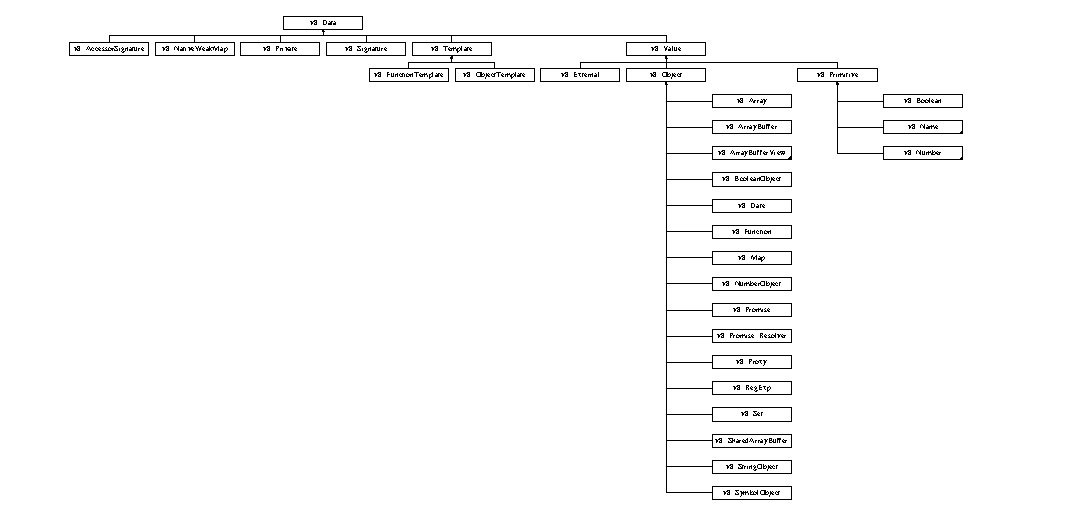
\includegraphics[height=6.491763cm]{classv8_1_1_data}
\end{center}
\end{figure}


\subsection{Detailed Description}
The superclass of values and A\+PI object templates. 

The documentation for this class was generated from the following file\+:\begin{DoxyCompactItemize}
\item 
include/v8.\+h\end{DoxyCompactItemize}

\hypertarget{classv8_1_1_data_view}{}\section{v8\+:\+:Data\+View Class Reference}
\label{classv8_1_1_data_view}\index{v8\+::\+Data\+View@{v8\+::\+Data\+View}}


{\ttfamily \#include $<$v8.\+h$>$}

Inheritance diagram for v8\+:\+:Data\+View\+:\begin{figure}[H]
\begin{center}
\leavevmode
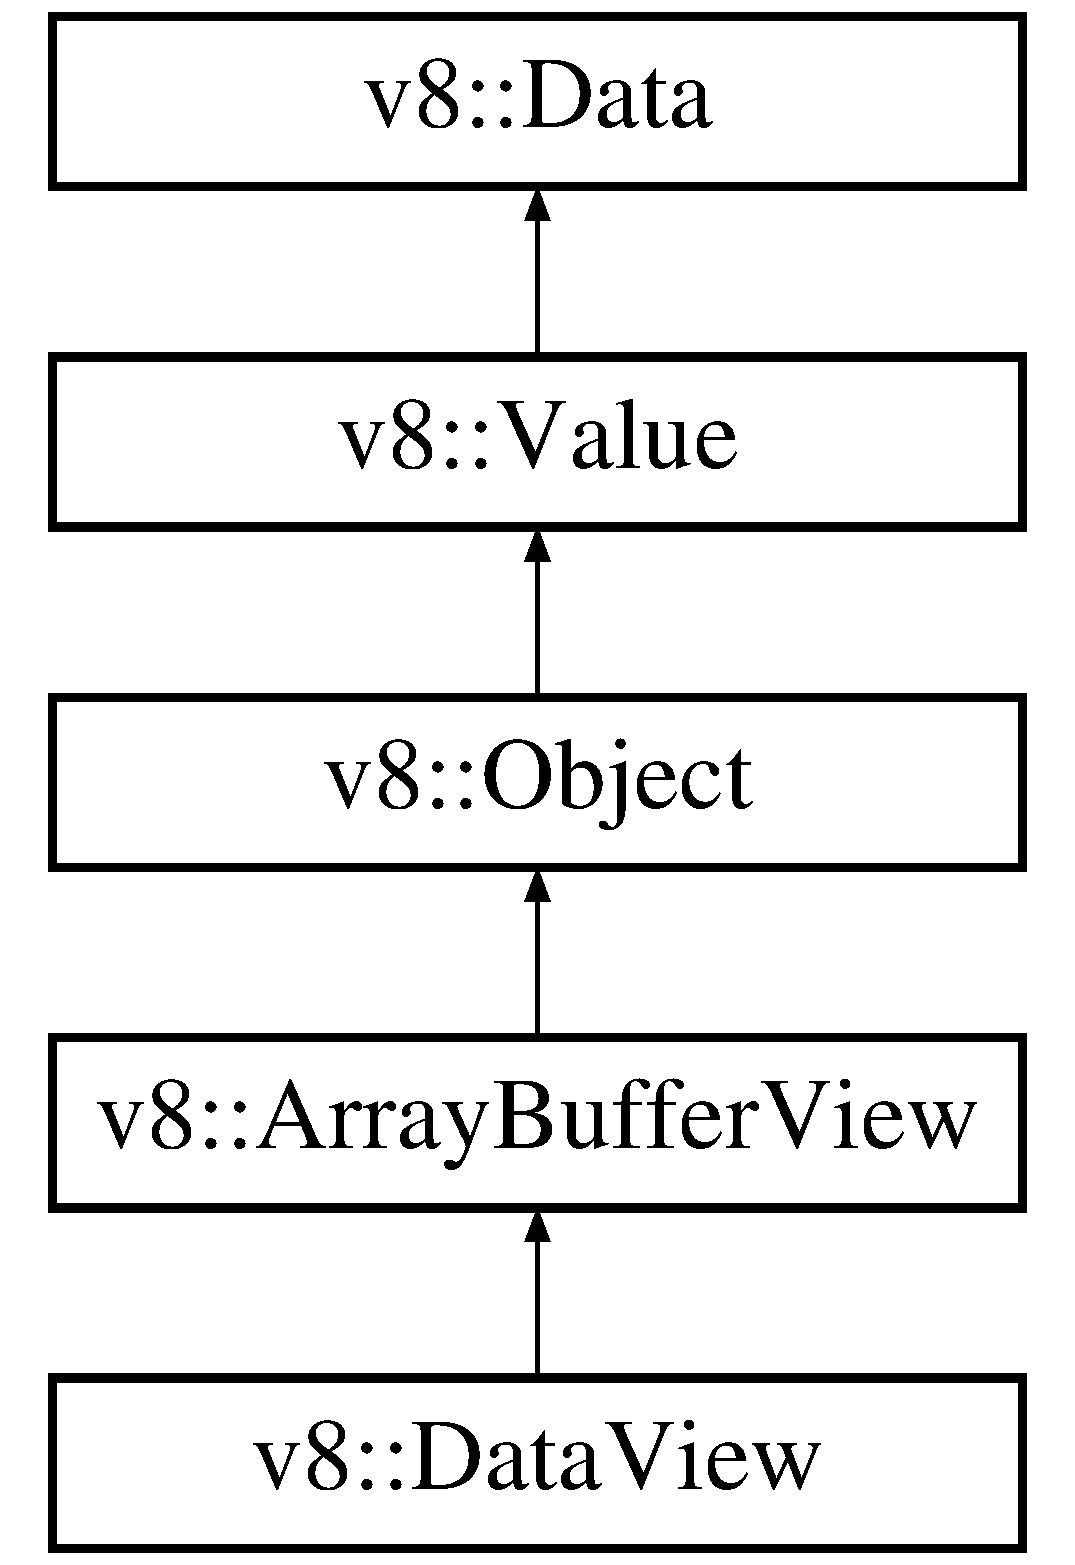
\includegraphics[height=5.000000cm]{classv8_1_1_data_view}
\end{center}
\end{figure}
\subsection*{Static Public Member Functions}
\begin{DoxyCompactItemize}
\item 
static \hyperlink{classv8_1_1_local}{Local}$<$ \hyperlink{classv8_1_1_data_view}{Data\+View} $>$ {\bfseries New} (\hyperlink{classv8_1_1_local}{Local}$<$ \hyperlink{classv8_1_1_array_buffer}{Array\+Buffer} $>$ array\+\_\+buffer, size\+\_\+t byte\+\_\+offset, size\+\_\+t length)\hypertarget{classv8_1_1_data_view_a40dcfc9ed56dbc41f48ddc49271cbab0}{}\label{classv8_1_1_data_view_a40dcfc9ed56dbc41f48ddc49271cbab0}

\item 
static \hyperlink{classv8_1_1_local}{Local}$<$ \hyperlink{classv8_1_1_data_view}{Data\+View} $>$ {\bfseries New} (\hyperlink{classv8_1_1_local}{Local}$<$ \hyperlink{classv8_1_1_shared_array_buffer}{Shared\+Array\+Buffer} $>$ shared\+\_\+array\+\_\+buffer, size\+\_\+t byte\+\_\+offset, size\+\_\+t length)\hypertarget{classv8_1_1_data_view_a8310e075564dd9f26122be2733995ba2}{}\label{classv8_1_1_data_view_a8310e075564dd9f26122be2733995ba2}

\item 
static V8\+\_\+\+I\+N\+L\+I\+NE \hyperlink{classv8_1_1_data_view}{Data\+View} $\ast$ {\bfseries Cast} (\hyperlink{classv8_1_1_value}{Value} $\ast$obj)\hypertarget{classv8_1_1_data_view_aa97d15fcb28c6c002a52d32877c8fd3a}{}\label{classv8_1_1_data_view_aa97d15fcb28c6c002a52d32877c8fd3a}

\end{DoxyCompactItemize}
\subsection*{Static Private Member Functions}
\begin{DoxyCompactItemize}
\item 
static void {\bfseries Check\+Cast} (\hyperlink{classv8_1_1_value}{Value} $\ast$obj)\hypertarget{classv8_1_1_data_view_ac7b128682169a4ac22395bfcbbb6b9f7}{}\label{classv8_1_1_data_view_ac7b128682169a4ac22395bfcbbb6b9f7}

\end{DoxyCompactItemize}
\subsection*{Additional Inherited Members}


\subsection{Detailed Description}
An instance of \hyperlink{classv8_1_1_data_view}{Data\+View} constructor (E\+S6 draft 15.\+13.\+7). This A\+PI is experimental and may change significantly. 

The documentation for this class was generated from the following file\+:\begin{DoxyCompactItemize}
\item 
/\+Users/joshgav/node/v8/include/v8.\+h\end{DoxyCompactItemize}

\hypertarget{classv8_1_1_date}{}\section{v8\+:\+:Date Class Reference}
\label{classv8_1_1_date}\index{v8\+::\+Date@{v8\+::\+Date}}


{\ttfamily \#include $<$v8.\+h$>$}

Inheritance diagram for v8\+:\+:Date\+:\begin{figure}[H]
\begin{center}
\leavevmode
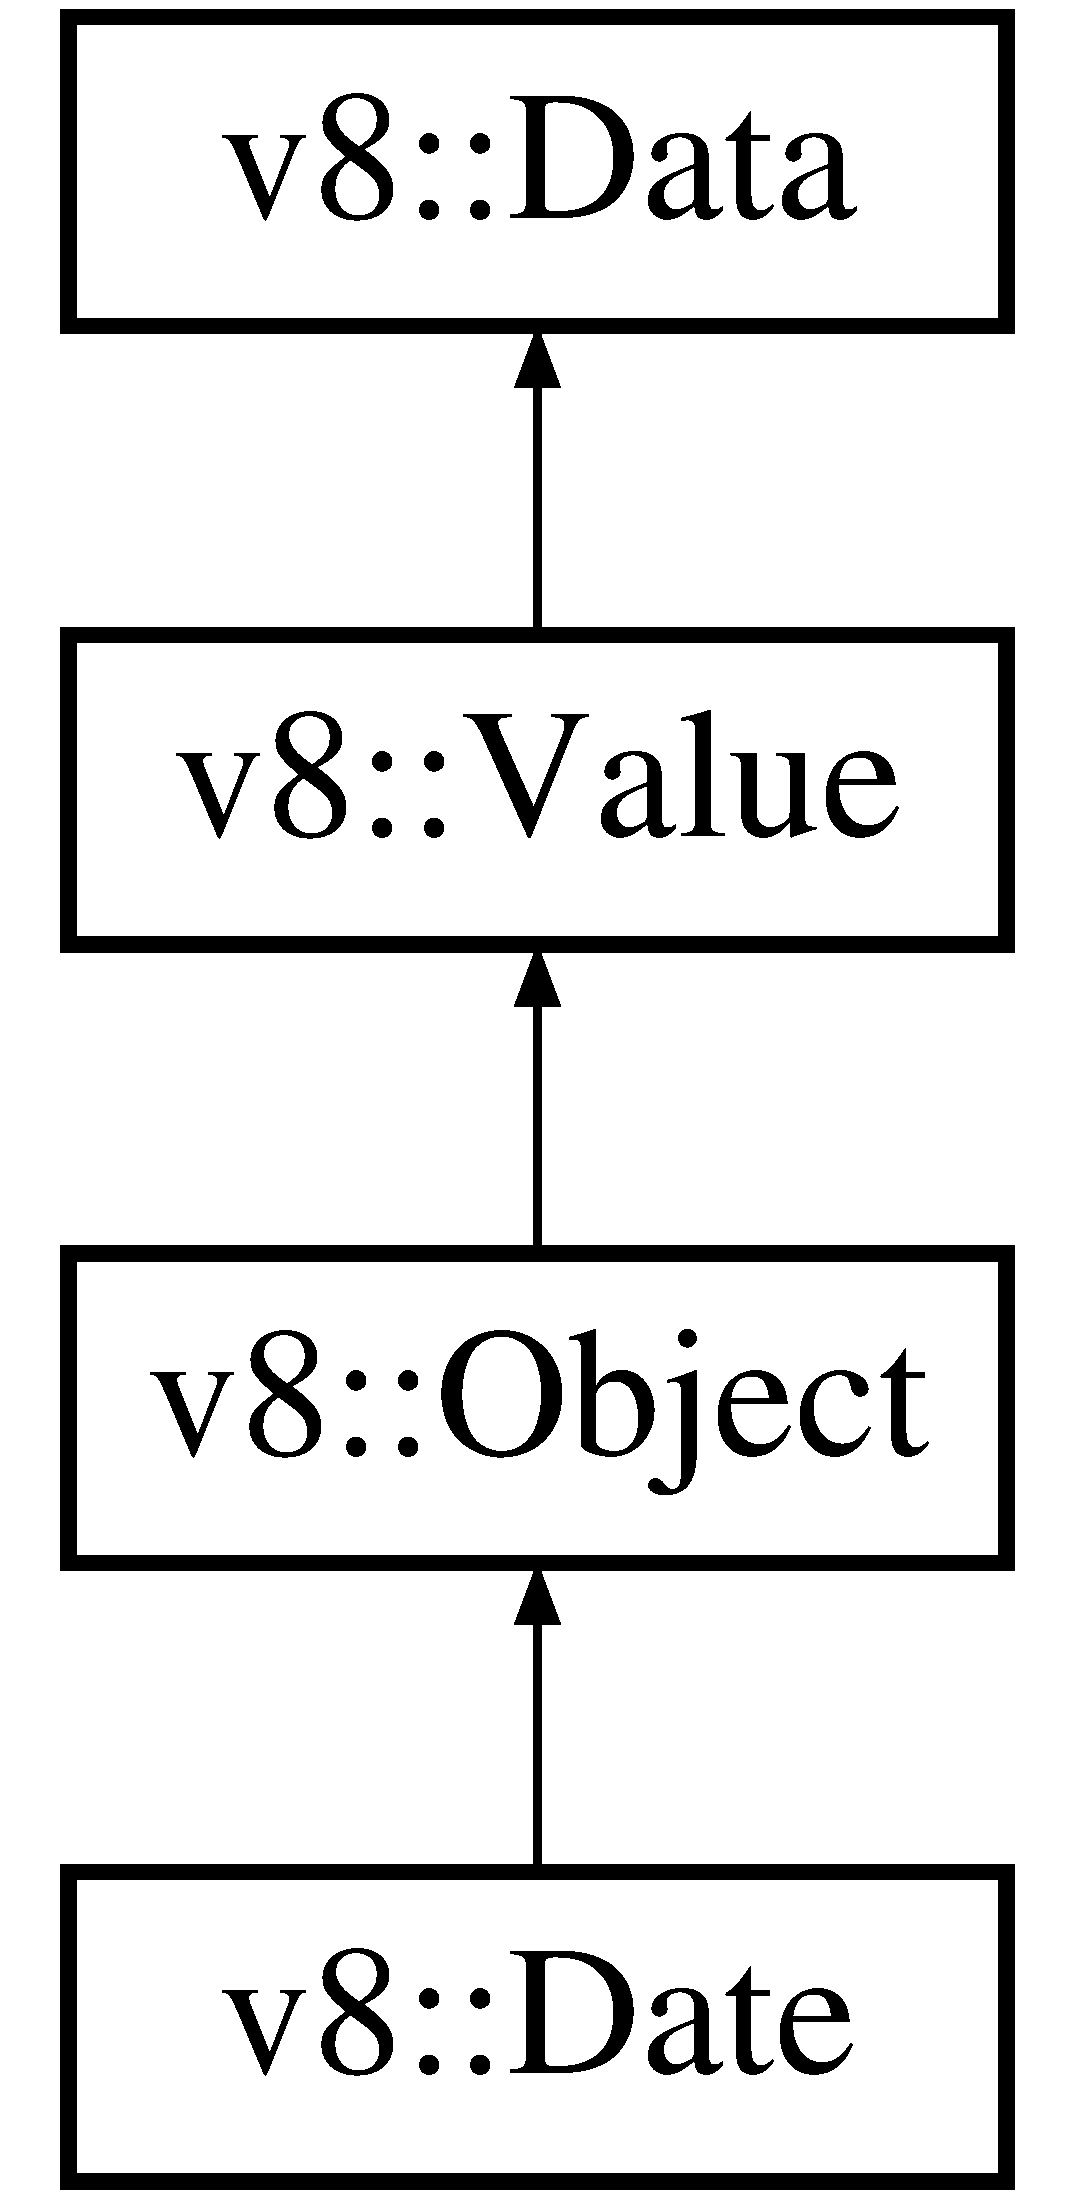
\includegraphics[height=4.000000cm]{classv8_1_1_date}
\end{center}
\end{figure}
\subsection*{Public Member Functions}
\begin{DoxyCompactItemize}
\item 
double \hyperlink{classv8_1_1_date_a06800409271fe5fa74202e0fd1ec8e87}{Value\+Of} () const 
\end{DoxyCompactItemize}
\subsection*{Static Public Member Functions}
\begin{DoxyCompactItemize}
\item 
static {\bfseries V8\+\_\+\+D\+E\+P\+R\+E\+C\+A\+T\+E\+\_\+\+S\+O\+ON} (\char`\"{}Use maybe version.\char`\"{}, Local$<$ \hyperlink{classv8_1_1_value}{Value} $>$ New(\hyperlink{classv8_1_1_isolate}{Isolate} $\ast$isolate, double time))\hypertarget{classv8_1_1_date_a4537a2f3b7de01ccc40784923ccece11}{}\label{classv8_1_1_date_a4537a2f3b7de01ccc40784923ccece11}

\item 
static V8\+\_\+\+W\+A\+R\+N\+\_\+\+U\+N\+U\+S\+E\+D\+\_\+\+R\+E\+S\+U\+LT \hyperlink{classv8_1_1_maybe_local}{Maybe\+Local}$<$ \hyperlink{classv8_1_1_value}{Value} $>$ {\bfseries New} (\hyperlink{classv8_1_1_local}{Local}$<$ \hyperlink{classv8_1_1_context}{Context} $>$ context, double time)\hypertarget{classv8_1_1_date_a07639d26ad5bc9564c2411a1c14f7d70}{}\label{classv8_1_1_date_a07639d26ad5bc9564c2411a1c14f7d70}

\item 
static V8\+\_\+\+I\+N\+L\+I\+NE \hyperlink{classv8_1_1_date}{Date} $\ast$ {\bfseries Cast} (\hyperlink{classv8_1_1_value}{v8\+::\+Value} $\ast$obj)\hypertarget{classv8_1_1_date_a8e5ea7c1f28924b82922270d6596b4d3}{}\label{classv8_1_1_date_a8e5ea7c1f28924b82922270d6596b4d3}

\item 
static void \hyperlink{classv8_1_1_date_adb084ec0683d3d195ad0f78af5f6f72b}{Date\+Time\+Configuration\+Change\+Notification} (\hyperlink{classv8_1_1_isolate}{Isolate} $\ast$isolate)
\end{DoxyCompactItemize}
\subsection*{Static Private Member Functions}
\begin{DoxyCompactItemize}
\item 
static void {\bfseries Check\+Cast} (\hyperlink{classv8_1_1_value}{v8\+::\+Value} $\ast$obj)\hypertarget{classv8_1_1_date_aa7bfe8c50da29286090aab105d459abb}{}\label{classv8_1_1_date_aa7bfe8c50da29286090aab105d459abb}

\end{DoxyCompactItemize}


\subsection{Detailed Description}
An instance of the built-\/in \hyperlink{classv8_1_1_date}{Date} constructor (E\+C\+M\+A-\/262, 15.\+9). 

\subsection{Member Function Documentation}
\index{v8\+::\+Date@{v8\+::\+Date}!Date\+Time\+Configuration\+Change\+Notification@{Date\+Time\+Configuration\+Change\+Notification}}
\index{Date\+Time\+Configuration\+Change\+Notification@{Date\+Time\+Configuration\+Change\+Notification}!v8\+::\+Date@{v8\+::\+Date}}
\subsubsection[{\texorpdfstring{Date\+Time\+Configuration\+Change\+Notification(\+Isolate $\ast$isolate)}{DateTimeConfigurationChangeNotification(Isolate *isolate)}}]{\setlength{\rightskip}{0pt plus 5cm}static void v8\+::\+Date\+::\+Date\+Time\+Configuration\+Change\+Notification (
\begin{DoxyParamCaption}
\item[{{\bf Isolate} $\ast$}]{isolate}
\end{DoxyParamCaption}
)\hspace{0.3cm}{\ttfamily [static]}}\hypertarget{classv8_1_1_date_adb084ec0683d3d195ad0f78af5f6f72b}{}\label{classv8_1_1_date_adb084ec0683d3d195ad0f78af5f6f72b}
Notification that the embedder has changed the time zone, daylight savings time, or other date / time configuration parameters. \hyperlink{classv8_1_1_v8}{V8} keeps a cache of various values used for date / time computation. This notification will reset those cached values for the current context so that date / time configuration changes would be reflected in the \hyperlink{classv8_1_1_date}{Date} object.

This A\+PI should not be called more than needed as it will negatively impact the performance of date operations. \index{v8\+::\+Date@{v8\+::\+Date}!Value\+Of@{Value\+Of}}
\index{Value\+Of@{Value\+Of}!v8\+::\+Date@{v8\+::\+Date}}
\subsubsection[{\texorpdfstring{Value\+Of() const }{ValueOf() const }}]{\setlength{\rightskip}{0pt plus 5cm}double v8\+::\+Date\+::\+Value\+Of (
\begin{DoxyParamCaption}
{}
\end{DoxyParamCaption}
) const}\hypertarget{classv8_1_1_date_a06800409271fe5fa74202e0fd1ec8e87}{}\label{classv8_1_1_date_a06800409271fe5fa74202e0fd1ec8e87}
A specialization of Value\+::\+Number\+Value that is more efficient because we know the structure of this object. 

The documentation for this class was generated from the following file\+:\begin{DoxyCompactItemize}
\item 
/\+Users/joshgav/node/v8/include/v8.\+h\end{DoxyCompactItemize}

\hypertarget{classv8_1_1_debug}{}\section{v8\+:\+:Debug Class Reference}
\label{classv8_1_1_debug}\index{v8\+::\+Debug@{v8\+::\+Debug}}
\subsection*{Classes}
\begin{DoxyCompactItemize}
\item 
class \hyperlink{classv8_1_1_debug_1_1_client_data}{Client\+Data}
\item 
class \hyperlink{classv8_1_1_debug_1_1_event_details}{Event\+Details}
\item 
class \hyperlink{classv8_1_1_debug_1_1_message}{Message}
\end{DoxyCompactItemize}
\subsection*{Public Types}
\begin{DoxyCompactItemize}
\item 
typedef void($\ast$ \hyperlink{classv8_1_1_debug_ab53894746a21222796062f0e81ea28d8}{Event\+Callback}) (const \hyperlink{classv8_1_1_debug_1_1_event_details}{Event\+Details} \&event\+\_\+details)
\item 
typedef void($\ast$ \hyperlink{classv8_1_1_debug_a526826b857bd3e3efa184e12bcebc694}{Message\+Handler}) (const \hyperlink{classv8_1_1_debug_1_1_message}{Message} \&message)
\item 
typedef void($\ast$ \hyperlink{classv8_1_1_debug_a91cd8aa9743e3478bc63fe73abcd557c}{Debug\+Message\+Dispatch\+Handler}) ()
\end{DoxyCompactItemize}
\subsection*{Public Member Functions}
\begin{DoxyCompactItemize}
\item 
{\bfseries V8\+\_\+\+D\+E\+P\+R\+E\+C\+A\+T\+ED} (\char`\"{}Use version with an \hyperlink{classv8_1_1_isolate}{Isolate}\char`\"{}, static bool Set\+Debug\+Event\+Listener(                                                                       \hyperlink{classv8_1_1_debug_ab53894746a21222796062f0e81ea28d8}{Event\+Callback} that, \hyperlink{classv8_1_1_local}{Local}$<$ \hyperlink{classv8_1_1_value}{Value} $>$ data=\hyperlink{classv8_1_1_local}{Local}$<$ \hyperlink{classv8_1_1_value}{Value} $>$()))\hypertarget{classv8_1_1_debug_a136072a1c36660385a4dd5e242588eff}{}\label{classv8_1_1_debug_a136072a1c36660385a4dd5e242588eff}

\item 
{\bfseries V8\+\_\+\+D\+E\+P\+R\+E\+C\+A\+T\+ED} (\char`\"{}Use version with an \hyperlink{classv8_1_1_isolate}{Isolate}\char`\"{}, static void Set\+Message\+Handler(\hyperlink{classv8_1_1_debug_a526826b857bd3e3efa184e12bcebc694}{Message\+Handler} handler))\hypertarget{classv8_1_1_debug_a47ea3e258dfe3539890b4a29859481e4}{}\label{classv8_1_1_debug_a47ea3e258dfe3539890b4a29859481e4}

\item 
{\bfseries V8\+\_\+\+D\+E\+P\+R\+E\+C\+A\+T\+ED} (\char`\"{}Use version with an \hyperlink{classv8_1_1_isolate}{Isolate}\char`\"{}, static void \hyperlink{classv8_1_1_debug_af005b911101260e0458847d149d5610e}{Process\+Debug\+Messages}())\hypertarget{classv8_1_1_debug_a5682cd506adcc344fe99b8c9b21bbac8}{}\label{classv8_1_1_debug_a5682cd506adcc344fe99b8c9b21bbac8}

\item 
{\bfseries V8\+\_\+\+D\+E\+P\+R\+E\+C\+A\+T\+ED} (\char`\"{}Use version with an \hyperlink{classv8_1_1_isolate}{Isolate}\char`\"{}, static \hyperlink{classv8_1_1_local}{Local}$<$ \hyperlink{classv8_1_1_context}{Context} $>$ \hyperlink{classv8_1_1_debug_abcf6727d68c5f8c35eef75a72e6a0da8}{Get\+Debug\+Context}())\hypertarget{classv8_1_1_debug_afe8bf40a79b8769cedfb7aafef74e77f}{}\label{classv8_1_1_debug_afe8bf40a79b8769cedfb7aafef74e77f}

\end{DoxyCompactItemize}
\subsection*{Static Public Member Functions}
\begin{DoxyCompactItemize}
\item 
static bool {\bfseries Set\+Debug\+Event\+Listener} (\hyperlink{classv8_1_1_isolate}{Isolate} $\ast$isolate, \hyperlink{classv8_1_1_debug_ab53894746a21222796062f0e81ea28d8}{Event\+Callback} that, \hyperlink{classv8_1_1_local}{Local}$<$ \hyperlink{classv8_1_1_value}{Value} $>$ data=\hyperlink{classv8_1_1_local}{Local}$<$ \hyperlink{classv8_1_1_value}{Value} $>$())\hypertarget{classv8_1_1_debug_a7f5138bd280a4c3fa9058a2d559687dd}{}\label{classv8_1_1_debug_a7f5138bd280a4c3fa9058a2d559687dd}

\item 
static void {\bfseries Debug\+Break} (\hyperlink{classv8_1_1_isolate}{Isolate} $\ast$isolate)\hypertarget{classv8_1_1_debug_a0c730ea558b1fc86cb728980c91a4c7c}{}\label{classv8_1_1_debug_a0c730ea558b1fc86cb728980c91a4c7c}

\item 
static void {\bfseries Cancel\+Debug\+Break} (\hyperlink{classv8_1_1_isolate}{Isolate} $\ast$isolate)\hypertarget{classv8_1_1_debug_a976a373dc06c146cdbe8d6f2fd7f57b5}{}\label{classv8_1_1_debug_a976a373dc06c146cdbe8d6f2fd7f57b5}

\item 
static bool {\bfseries Check\+Debug\+Break} (\hyperlink{classv8_1_1_isolate}{Isolate} $\ast$isolate)\hypertarget{classv8_1_1_debug_aa564431664efa61d6d72c9cbd91b4ea2}{}\label{classv8_1_1_debug_aa564431664efa61d6d72c9cbd91b4ea2}

\item 
static void {\bfseries Set\+Message\+Handler} (\hyperlink{classv8_1_1_isolate}{Isolate} $\ast$isolate, \hyperlink{classv8_1_1_debug_a526826b857bd3e3efa184e12bcebc694}{Message\+Handler} handler)\hypertarget{classv8_1_1_debug_ae49147c056122437bacc3d26cc349125}{}\label{classv8_1_1_debug_ae49147c056122437bacc3d26cc349125}

\item 
static void {\bfseries Send\+Command} (\hyperlink{classv8_1_1_isolate}{Isolate} $\ast$isolate, const uint16\+\_\+t $\ast$command, int length, \hyperlink{classv8_1_1_debug_1_1_client_data}{Client\+Data} $\ast$client\+\_\+data=N\+U\+LL)\hypertarget{classv8_1_1_debug_aba2426f25ee7cd31659426287777bb00}{}\label{classv8_1_1_debug_aba2426f25ee7cd31659426287777bb00}

\item 
static \hyperlink{classv8_1_1_debug_a5c53fc48b3fca71b6397cfecd1c82a9d}{V8\+\_\+\+D\+E\+P\+R\+E\+C\+A\+T\+ED} (\char`\"{}Use maybe version\char`\"{}, Local$<$ \hyperlink{classv8_1_1_value}{Value} $>$ Call(\hyperlink{classv8_1_1_local}{v8\+::\+Local}$<$ \hyperlink{classv8_1_1_function}{v8\+::\+Function} $>$ fun,                                                                                                                                                           \hyperlink{classv8_1_1_local}{Local}$<$ \hyperlink{classv8_1_1_value}{Value} $>$ data=\hyperlink{classv8_1_1_local}{Local}$<$ \hyperlink{classv8_1_1_value}{Value} $>$()))
\item 
static \hyperlink{classv8_1_1_maybe_local}{Maybe\+Local}$<$ \hyperlink{classv8_1_1_value}{Value} $>$ {\bfseries Call} (\hyperlink{classv8_1_1_local}{Local}$<$ \hyperlink{classv8_1_1_context}{Context} $>$ context, \hyperlink{classv8_1_1_local}{v8\+::\+Local}$<$ \hyperlink{classv8_1_1_function}{v8\+::\+Function} $>$ fun, \hyperlink{classv8_1_1_local}{Local}$<$ \hyperlink{classv8_1_1_value}{Value} $>$ data=\hyperlink{classv8_1_1_local}{Local}$<$ \hyperlink{classv8_1_1_value}{Value} $>$())\hypertarget{classv8_1_1_debug_a32e28ec40dc429e7fa1dfbe1e514ba3d}{}\label{classv8_1_1_debug_a32e28ec40dc429e7fa1dfbe1e514ba3d}

\item 
static \hyperlink{classv8_1_1_debug_aeda86872fb9c66df641e6d16c8db7182}{V8\+\_\+\+D\+E\+P\+R\+E\+C\+A\+T\+ED} (\char`\"{}Use maybe version\char`\"{}, Local$<$ \hyperlink{classv8_1_1_value}{Value} $>$ Get\+Mirror(\hyperlink{classv8_1_1_local}{v8\+::\+Local}$<$ \hyperlink{classv8_1_1_value}{v8\+::\+Value} $>$ obj))
\item 
static \hyperlink{classv8_1_1_maybe_local}{Maybe\+Local}$<$ \hyperlink{classv8_1_1_value}{Value} $>$ {\bfseries Get\+Mirror} (\hyperlink{classv8_1_1_local}{Local}$<$ \hyperlink{classv8_1_1_context}{Context} $>$ context, \hyperlink{classv8_1_1_local}{v8\+::\+Local}$<$ \hyperlink{classv8_1_1_value}{v8\+::\+Value} $>$ obj)\hypertarget{classv8_1_1_debug_ab5f5ae3f4418c576da4633c6fb27b23d}{}\label{classv8_1_1_debug_ab5f5ae3f4418c576da4633c6fb27b23d}

\item 
static void \hyperlink{classv8_1_1_debug_af005b911101260e0458847d149d5610e}{Process\+Debug\+Messages} (\hyperlink{classv8_1_1_isolate}{Isolate} $\ast$isolate)
\item 
static \hyperlink{classv8_1_1_local}{Local}$<$ \hyperlink{classv8_1_1_context}{Context} $>$ \hyperlink{classv8_1_1_debug_abcf6727d68c5f8c35eef75a72e6a0da8}{Get\+Debug\+Context} (\hyperlink{classv8_1_1_isolate}{Isolate} $\ast$isolate)
\item 
static void \hyperlink{classv8_1_1_debug_ab635f979d369bed13187e2594d825517}{Set\+Live\+Edit\+Enabled} (\hyperlink{classv8_1_1_isolate}{Isolate} $\ast$isolate, bool enable)
\item 
static \hyperlink{classv8_1_1_maybe_local}{Maybe\+Local}$<$ \hyperlink{classv8_1_1_array}{Array} $>$ \hyperlink{classv8_1_1_debug_a10ef14b11ffdd57287f25b39dc728e07}{Get\+Internal\+Properties} (\hyperlink{classv8_1_1_isolate}{Isolate} $\ast$isolate, \hyperlink{classv8_1_1_local}{Local}$<$ \hyperlink{classv8_1_1_value}{Value} $>$ value)
\item 
static bool \hyperlink{classv8_1_1_debug_a79ce7b9e4e09be64ca1c3494ec6130ab}{Is\+Tail\+Call\+Elimination\+Enabled} (\hyperlink{classv8_1_1_isolate}{Isolate} $\ast$isolate)
\item 
static void {\bfseries Set\+Tail\+Call\+Elimination\+Enabled} (\hyperlink{classv8_1_1_isolate}{Isolate} $\ast$isolate, bool enabled)\hypertarget{classv8_1_1_debug_a06662e09d22d6eaed81f20824066cea5}{}\label{classv8_1_1_debug_a06662e09d22d6eaed81f20824066cea5}

\end{DoxyCompactItemize}


\subsection{Member Typedef Documentation}
\index{v8\+::\+Debug@{v8\+::\+Debug}!Debug\+Message\+Dispatch\+Handler@{Debug\+Message\+Dispatch\+Handler}}
\index{Debug\+Message\+Dispatch\+Handler@{Debug\+Message\+Dispatch\+Handler}!v8\+::\+Debug@{v8\+::\+Debug}}
\subsubsection[{\texorpdfstring{Debug\+Message\+Dispatch\+Handler}{DebugMessageDispatchHandler}}]{\setlength{\rightskip}{0pt plus 5cm}typedef void($\ast$ v8\+::\+Debug\+::\+Debug\+Message\+Dispatch\+Handler) ()}\hypertarget{classv8_1_1_debug_a91cd8aa9743e3478bc63fe73abcd557c}{}\label{classv8_1_1_debug_a91cd8aa9743e3478bc63fe73abcd557c}
Callback function for the host to ensure debug messages are processed. \index{v8\+::\+Debug@{v8\+::\+Debug}!Event\+Callback@{Event\+Callback}}
\index{Event\+Callback@{Event\+Callback}!v8\+::\+Debug@{v8\+::\+Debug}}
\subsubsection[{\texorpdfstring{Event\+Callback}{EventCallback}}]{\setlength{\rightskip}{0pt plus 5cm}typedef void($\ast$ v8\+::\+Debug\+::\+Event\+Callback) (const {\bf Event\+Details} \&event\+\_\+details)}\hypertarget{classv8_1_1_debug_ab53894746a21222796062f0e81ea28d8}{}\label{classv8_1_1_debug_ab53894746a21222796062f0e81ea28d8}
\hyperlink{classv8_1_1_debug}{Debug} event callback function.


\begin{DoxyParams}{Parameters}
{\em event\+\_\+details} & object providing information about the debug event\\
\hline
\end{DoxyParams}
A Event\+Callback2 does not take possession of the event data, and must not rely on the data persisting after the handler returns. \index{v8\+::\+Debug@{v8\+::\+Debug}!Message\+Handler@{Message\+Handler}}
\index{Message\+Handler@{Message\+Handler}!v8\+::\+Debug@{v8\+::\+Debug}}
\subsubsection[{\texorpdfstring{Message\+Handler}{MessageHandler}}]{\setlength{\rightskip}{0pt plus 5cm}typedef void($\ast$ v8\+::\+Debug\+::\+Message\+Handler) (const {\bf Message} \&message)}\hypertarget{classv8_1_1_debug_a526826b857bd3e3efa184e12bcebc694}{}\label{classv8_1_1_debug_a526826b857bd3e3efa184e12bcebc694}
\hyperlink{classv8_1_1_debug}{Debug} message callback function.


\begin{DoxyParams}{Parameters}
{\em message} & the debug message handler message object\\
\hline
\end{DoxyParams}
A Message\+Handler2 does not take possession of the message data, and must not rely on the data persisting after the handler returns. 

\subsection{Member Function Documentation}
\index{v8\+::\+Debug@{v8\+::\+Debug}!Get\+Debug\+Context@{Get\+Debug\+Context}}
\index{Get\+Debug\+Context@{Get\+Debug\+Context}!v8\+::\+Debug@{v8\+::\+Debug}}
\subsubsection[{\texorpdfstring{Get\+Debug\+Context(\+Isolate $\ast$isolate)}{GetDebugContext(Isolate *isolate)}}]{\setlength{\rightskip}{0pt plus 5cm}static {\bf Local}$<${\bf Context}$>$ v8\+::\+Debug\+::\+Get\+Debug\+Context (
\begin{DoxyParamCaption}
\item[{{\bf Isolate} $\ast$}]{isolate}
\end{DoxyParamCaption}
)\hspace{0.3cm}{\ttfamily [static]}}\hypertarget{classv8_1_1_debug_abcf6727d68c5f8c35eef75a72e6a0da8}{}\label{classv8_1_1_debug_abcf6727d68c5f8c35eef75a72e6a0da8}
Debugger is running in its own context which is entered while debugger messages are being dispatched. This is an explicit getter for this debugger context. Note that the content of the debugger context is subject to change. The \hyperlink{classv8_1_1_context}{Context} exists only when the debugger is active, i.\+e. at least one Debug\+Event\+Listener or Message\+Handler is set. \index{v8\+::\+Debug@{v8\+::\+Debug}!Get\+Internal\+Properties@{Get\+Internal\+Properties}}
\index{Get\+Internal\+Properties@{Get\+Internal\+Properties}!v8\+::\+Debug@{v8\+::\+Debug}}
\subsubsection[{\texorpdfstring{Get\+Internal\+Properties(\+Isolate $\ast$isolate, Local$<$ Value $>$ value)}{GetInternalProperties(Isolate *isolate, Local< Value > value)}}]{\setlength{\rightskip}{0pt plus 5cm}static {\bf Maybe\+Local}$<${\bf Array}$>$ v8\+::\+Debug\+::\+Get\+Internal\+Properties (
\begin{DoxyParamCaption}
\item[{{\bf Isolate} $\ast$}]{isolate, }
\item[{{\bf Local}$<$ {\bf Value} $>$}]{value}
\end{DoxyParamCaption}
)\hspace{0.3cm}{\ttfamily [static]}}\hypertarget{classv8_1_1_debug_a10ef14b11ffdd57287f25b39dc728e07}{}\label{classv8_1_1_debug_a10ef14b11ffdd57287f25b39dc728e07}
Returns array of internal properties specific to the value type. Result has the following format\+: \mbox{[}$<$name$>$, 

,...,$<$name$>$, 

\mbox{]}. Result array will be allocated in the current context. \index{v8\+::\+Debug@{v8\+::\+Debug}!Is\+Tail\+Call\+Elimination\+Enabled@{Is\+Tail\+Call\+Elimination\+Enabled}}
\index{Is\+Tail\+Call\+Elimination\+Enabled@{Is\+Tail\+Call\+Elimination\+Enabled}!v8\+::\+Debug@{v8\+::\+Debug}}
\subsubsection[{\texorpdfstring{Is\+Tail\+Call\+Elimination\+Enabled(\+Isolate $\ast$isolate)}{IsTailCallEliminationEnabled(Isolate *isolate)}}]{\setlength{\rightskip}{0pt plus 5cm}static bool v8\+::\+Debug\+::\+Is\+Tail\+Call\+Elimination\+Enabled (
\begin{DoxyParamCaption}
\item[{{\bf Isolate} $\ast$}]{isolate}
\end{DoxyParamCaption}
)\hspace{0.3cm}{\ttfamily [static]}}\hypertarget{classv8_1_1_debug_a79ce7b9e4e09be64ca1c3494ec6130ab}{}\label{classv8_1_1_debug_a79ce7b9e4e09be64ca1c3494ec6130ab}
Defines if the E\+S2015 tail call elimination feature is enabled or not. The change of this flag triggers deoptimization of all functions that contain calls at tail position. \index{v8\+::\+Debug@{v8\+::\+Debug}!Process\+Debug\+Messages@{Process\+Debug\+Messages}}
\index{Process\+Debug\+Messages@{Process\+Debug\+Messages}!v8\+::\+Debug@{v8\+::\+Debug}}
\subsubsection[{\texorpdfstring{Process\+Debug\+Messages(\+Isolate $\ast$isolate)}{ProcessDebugMessages(Isolate *isolate)}}]{\setlength{\rightskip}{0pt plus 5cm}static void v8\+::\+Debug\+::\+Process\+Debug\+Messages (
\begin{DoxyParamCaption}
\item[{{\bf Isolate} $\ast$}]{isolate}
\end{DoxyParamCaption}
)\hspace{0.3cm}{\ttfamily [static]}}\hypertarget{classv8_1_1_debug_af005b911101260e0458847d149d5610e}{}\label{classv8_1_1_debug_af005b911101260e0458847d149d5610e}
Makes \hyperlink{classv8_1_1_v8}{V8} process all pending debug messages.

From \hyperlink{classv8_1_1_v8}{V8} point of view all debug messages come asynchronously (e.\+g. from remote debugger) but they all must be handled synchronously\+: \hyperlink{classv8_1_1_v8}{V8} cannot do 2 things at one time so normal script execution must be interrupted for a while.

Generally when message arrives \hyperlink{classv8_1_1_v8}{V8} may be in one of 3 states\+:
\begin{DoxyEnumerate}
\item \hyperlink{classv8_1_1_v8}{V8} is running script; \hyperlink{classv8_1_1_v8}{V8} will automatically interrupt and process all pending messages;
\item \hyperlink{classv8_1_1_v8}{V8} is suspended on debug breakpoint; in this state \hyperlink{classv8_1_1_v8}{V8} is dedicated to reading and processing debug messages;
\item \hyperlink{classv8_1_1_v8}{V8} is not running at all or has called some long-\/working C++ function; by default it means that processing of all debug messages will be deferred until \hyperlink{classv8_1_1_v8}{V8} gets control again; however, embedding application may improve this by manually calling this method.
\end{DoxyEnumerate}

Technically this method in many senses is equivalent to executing empty script\+:
\begin{DoxyEnumerate}
\item It does nothing except for processing all pending debug messages.
\item It should be invoked with the same precautions and from the same context as \hyperlink{classv8_1_1_v8}{V8} script would be invoked from, because\+: a. with \char`\"{}evaluate\char`\"{} command it can do whatever normal script can do, including all native calls; b. no other thread should call \hyperlink{classv8_1_1_v8}{V8} while this method is running (\hyperlink{classv8_1_1_locker}{v8\+::\+Locker} may be used here).
\end{DoxyEnumerate}

\char`\"{}\+Evaluate\char`\"{} debug command behavior currently is not specified in scope of this method. \index{v8\+::\+Debug@{v8\+::\+Debug}!Set\+Live\+Edit\+Enabled@{Set\+Live\+Edit\+Enabled}}
\index{Set\+Live\+Edit\+Enabled@{Set\+Live\+Edit\+Enabled}!v8\+::\+Debug@{v8\+::\+Debug}}
\subsubsection[{\texorpdfstring{Set\+Live\+Edit\+Enabled(\+Isolate $\ast$isolate, bool enable)}{SetLiveEditEnabled(Isolate *isolate, bool enable)}}]{\setlength{\rightskip}{0pt plus 5cm}static void v8\+::\+Debug\+::\+Set\+Live\+Edit\+Enabled (
\begin{DoxyParamCaption}
\item[{{\bf Isolate} $\ast$}]{isolate, }
\item[{bool}]{enable}
\end{DoxyParamCaption}
)\hspace{0.3cm}{\ttfamily [static]}}\hypertarget{classv8_1_1_debug_ab635f979d369bed13187e2594d825517}{}\label{classv8_1_1_debug_ab635f979d369bed13187e2594d825517}
Enable/disable Live\+Edit functionality for the given \hyperlink{classv8_1_1_isolate}{Isolate} (default \hyperlink{classv8_1_1_isolate}{Isolate} if not provided). \hyperlink{classv8_1_1_v8}{V8} will abort if Live\+Edit is unexpectedly used. Live\+Edit is enabled by default. \index{v8\+::\+Debug@{v8\+::\+Debug}!V8\+\_\+\+D\+E\+P\+R\+E\+C\+A\+T\+ED@{V8\+\_\+\+D\+E\+P\+R\+E\+C\+A\+T\+ED}}
\index{V8\+\_\+\+D\+E\+P\+R\+E\+C\+A\+T\+ED@{V8\+\_\+\+D\+E\+P\+R\+E\+C\+A\+T\+ED}!v8\+::\+Debug@{v8\+::\+Debug}}
\subsubsection[{\texorpdfstring{V8\+\_\+\+D\+E\+P\+R\+E\+C\+A\+T\+E\+D(""Use maybe version"", Local$<$ Value $>$ Call(v8\+::\+Local$<$ v8\+::\+Function $>$ fun,                                                                                                                                                           Local$<$ Value $>$ data=\+Local$<$ Value $>$()))}{V8_DEPRECATED("Use maybe version", Local< Value > Call(v8::Local< v8::Function > fun,                                                                                                                                                           Local< Value > data=Local< Value >()))}}]{\setlength{\rightskip}{0pt plus 5cm}static v8\+::\+Debug\+::\+V8\+\_\+\+D\+E\+P\+R\+E\+C\+A\+T\+ED (
\begin{DoxyParamCaption}
\item[{\char`\"{}Use maybe version\char`\"{}}]{, }
\item[{{\bf Local}$<$ {\bf Value} $>$ }]{Callv8\+::\+Local$<$ v8\+::\+Function $>$ fun,                                                                                                                                                                                                                                                                                                                   Local$<$ Value $>$ data=\+Local$<$ Value $>$()}
\end{DoxyParamCaption}
)\hspace{0.3cm}{\ttfamily [static]}}\hypertarget{classv8_1_1_debug_a5c53fc48b3fca71b6397cfecd1c82a9d}{}\label{classv8_1_1_debug_a5c53fc48b3fca71b6397cfecd1c82a9d}
Run a Java\+Script function in the debugger. 
\begin{DoxyParams}{Parameters}
{\em fun} & the function to call \\
\hline
{\em data} & passed as second argument to the function With this call the debugger is entered and the function specified is called with the execution state as the first argument. This makes it possible to get access to information otherwise not available during normal Java\+Script execution e.\+g. details on stack frames. Receiver of the function call will be the debugger context global object, however this is a subject to change. The following example shows a Java\+Script function which when passed to v8\+::\+Debug\+::\+Call will return the current line of Java\+Script execution.\\
\hline
\end{DoxyParams}

\begin{DoxyCode}
\textcolor{keyword}{function} frame\_source\_line(exec\_state) \{
  \textcolor{keywordflow}{return} exec\_state.frame(0).sourceLine();
\}
\end{DoxyCode}
 \index{v8\+::\+Debug@{v8\+::\+Debug}!V8\+\_\+\+D\+E\+P\+R\+E\+C\+A\+T\+ED@{V8\+\_\+\+D\+E\+P\+R\+E\+C\+A\+T\+ED}}
\index{V8\+\_\+\+D\+E\+P\+R\+E\+C\+A\+T\+ED@{V8\+\_\+\+D\+E\+P\+R\+E\+C\+A\+T\+ED}!v8\+::\+Debug@{v8\+::\+Debug}}
\subsubsection[{\texorpdfstring{V8\+\_\+\+D\+E\+P\+R\+E\+C\+A\+T\+E\+D(""Use maybe version"", Local$<$ Value $>$ Get\+Mirror(v8\+::\+Local$<$ v8\+::\+Value $>$ obj))}{V8_DEPRECATED("Use maybe version", Local< Value > GetMirror(v8::Local< v8::Value > obj))}}]{\setlength{\rightskip}{0pt plus 5cm}static v8\+::\+Debug\+::\+V8\+\_\+\+D\+E\+P\+R\+E\+C\+A\+T\+ED (
\begin{DoxyParamCaption}
\item[{\char`\"{}Use maybe version\char`\"{}}]{, }
\item[{{\bf Local}$<$ {\bf Value} $>$ }]{Get\+Mirrorv8\+::\+Local$<$ v8\+::\+Value $>$ obj}
\end{DoxyParamCaption}
)\hspace{0.3cm}{\ttfamily [static]}}\hypertarget{classv8_1_1_debug_aeda86872fb9c66df641e6d16c8db7182}{}\label{classv8_1_1_debug_aeda86872fb9c66df641e6d16c8db7182}
Returns a mirror object for the given object. 

The documentation for this class was generated from the following file\+:\begin{DoxyCompactItemize}
\item 
include/v8-\/debug.\+h\end{DoxyCompactItemize}

\hypertarget{classv8_1_1_default_global_map_traits}{}\section{v8\+:\+:Default\+Global\+Map\+Traits$<$ K, V $>$ Class Template Reference}
\label{classv8_1_1_default_global_map_traits}\index{v8\+::\+Default\+Global\+Map\+Traits$<$ K, V $>$@{v8\+::\+Default\+Global\+Map\+Traits$<$ K, V $>$}}
Inheritance diagram for v8\+:\+:Default\+Global\+Map\+Traits$<$ K, V $>$\+:\begin{figure}[H]
\begin{center}
\leavevmode
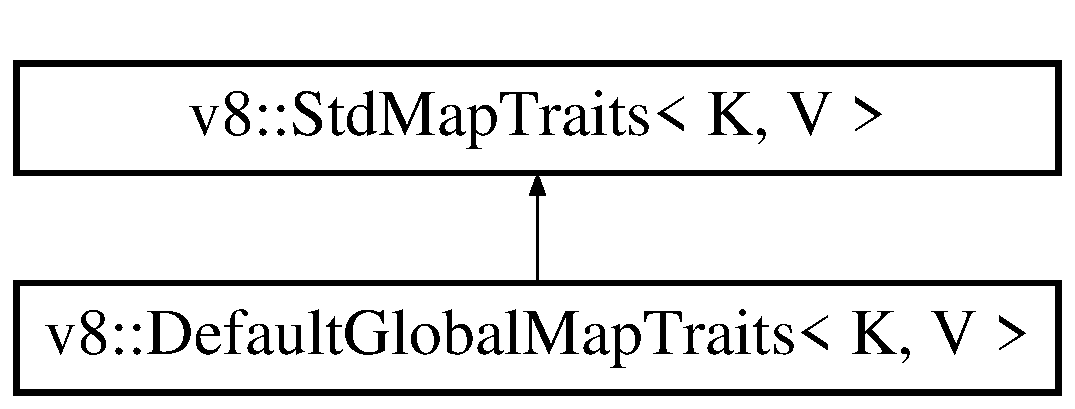
\includegraphics[height=2.000000cm]{classv8_1_1_default_global_map_traits}
\end{center}
\end{figure}
\subsection*{Classes}
\begin{DoxyCompactItemize}
\item 
struct \hyperlink{structv8_1_1_default_global_map_traits_1_1_remove_pointer}{Remove\+Pointer}
\item 
struct \hyperlink{structv8_1_1_default_global_map_traits_1_1_remove_pointer_3_01_t_01_5_01_4}{Remove\+Pointer$<$ T $\ast$ $>$}
\end{DoxyCompactItemize}
\subsection*{Public Types}
\begin{DoxyCompactItemize}
\item 
typedef \hyperlink{classv8_1_1_global_value_map}{Global\+Value\+Map}$<$ K, V, \hyperlink{classv8_1_1_default_global_map_traits}{Default\+Global\+Map\+Traits}$<$ K, V $>$ $>$ {\bfseries Map\+Type}\hypertarget{classv8_1_1_default_global_map_traits_a6626b089621a436fde5ac1a1132cc83c}{}\label{classv8_1_1_default_global_map_traits_a6626b089621a436fde5ac1a1132cc83c}

\item 
typedef void {\bfseries Weak\+Callback\+Data\+Type}\hypertarget{classv8_1_1_default_global_map_traits_af5285197aae83dcb00d0381fbc90869e}{}\label{classv8_1_1_default_global_map_traits_af5285197aae83dcb00d0381fbc90869e}

\end{DoxyCompactItemize}
\subsection*{Static Public Member Functions}
\begin{DoxyCompactItemize}
\item 
static Weak\+Callback\+Data\+Type $\ast$ {\bfseries Weak\+Callback\+Parameter} (\hyperlink{classv8_1_1_global_value_map}{Map\+Type} $\ast$map, const K \&key, \hyperlink{classv8_1_1_local}{Local}$<$ V $>$ value)\hypertarget{classv8_1_1_default_global_map_traits_a3d4b483a077d6e5665cc62a23c719ee8}{}\label{classv8_1_1_default_global_map_traits_a3d4b483a077d6e5665cc62a23c719ee8}

\item 
static \hyperlink{classv8_1_1_global_value_map}{Map\+Type} $\ast$ {\bfseries Map\+From\+Weak\+Callback\+Info} (const \hyperlink{classv8_1_1_weak_callback_info}{Weak\+Callback\+Info}$<$ Weak\+Callback\+Data\+Type $>$ \&data)\hypertarget{classv8_1_1_default_global_map_traits_ae65c4d78f93d033712aa328654c00250}{}\label{classv8_1_1_default_global_map_traits_ae65c4d78f93d033712aa328654c00250}

\item 
static K {\bfseries Key\+From\+Weak\+Callback\+Info} (const \hyperlink{classv8_1_1_weak_callback_info}{Weak\+Callback\+Info}$<$ Weak\+Callback\+Data\+Type $>$ \&data)\hypertarget{classv8_1_1_default_global_map_traits_a2ebc8d3bbfbe32598863ab44caa36207}{}\label{classv8_1_1_default_global_map_traits_a2ebc8d3bbfbe32598863ab44caa36207}

\item 
static void {\bfseries Dispose\+Callback\+Data} (Weak\+Callback\+Data\+Type $\ast$data)\hypertarget{classv8_1_1_default_global_map_traits_a106883e8168f48826fcfb71aa88e7994}{}\label{classv8_1_1_default_global_map_traits_a106883e8168f48826fcfb71aa88e7994}

\item 
static void {\bfseries On\+Weak\+Callback} (const \hyperlink{classv8_1_1_weak_callback_info}{Weak\+Callback\+Info}$<$ Weak\+Callback\+Data\+Type $>$ \&data)\hypertarget{classv8_1_1_default_global_map_traits_a2e50fabc65cf498e981015c1e92ece3e}{}\label{classv8_1_1_default_global_map_traits_a2e50fabc65cf498e981015c1e92ece3e}

\item 
static void {\bfseries Dispose} (\hyperlink{classv8_1_1_isolate}{Isolate} $\ast$isolate, \hyperlink{classv8_1_1_global}{Global}$<$ V $>$ value, K key)\hypertarget{classv8_1_1_default_global_map_traits_af2a539ddbe5db2b6e1e944590e1dd7e6}{}\label{classv8_1_1_default_global_map_traits_af2a539ddbe5db2b6e1e944590e1dd7e6}

\item 
static void {\bfseries Dispose\+Weak} (const \hyperlink{classv8_1_1_weak_callback_info}{Weak\+Callback\+Info}$<$ Weak\+Callback\+Data\+Type $>$ \&data)\hypertarget{classv8_1_1_default_global_map_traits_ad3478535925c0f42664c97c4d35d1c91}{}\label{classv8_1_1_default_global_map_traits_ad3478535925c0f42664c97c4d35d1c91}

\end{DoxyCompactItemize}
\subsection*{Static Public Attributes}
\begin{DoxyCompactItemize}
\item 
static const Persistent\+Container\+Callback\+Type {\bfseries k\+Callback\+Type} = k\+Not\+Weak\hypertarget{classv8_1_1_default_global_map_traits_aca4a466a95927f10ea3fa0bff1e041d2}{}\label{classv8_1_1_default_global_map_traits_aca4a466a95927f10ea3fa0bff1e041d2}

\end{DoxyCompactItemize}


The documentation for this class was generated from the following file\+:\begin{DoxyCompactItemize}
\item 
include/v8-\/util.\+h\end{DoxyCompactItemize}

\hypertarget{classv8_1_1_default_persistent_value_map_traits}{}\section{v8\+:\+:Default\+Persistent\+Value\+Map\+Traits$<$ K, V $>$ Class Template Reference}
\label{classv8_1_1_default_persistent_value_map_traits}\index{v8\+::\+Default\+Persistent\+Value\+Map\+Traits$<$ K, V $>$@{v8\+::\+Default\+Persistent\+Value\+Map\+Traits$<$ K, V $>$}}


{\ttfamily \#include $<$v8-\/util.\+h$>$}

Inheritance diagram for v8\+:\+:Default\+Persistent\+Value\+Map\+Traits$<$ K, V $>$\+:\begin{figure}[H]
\begin{center}
\leavevmode
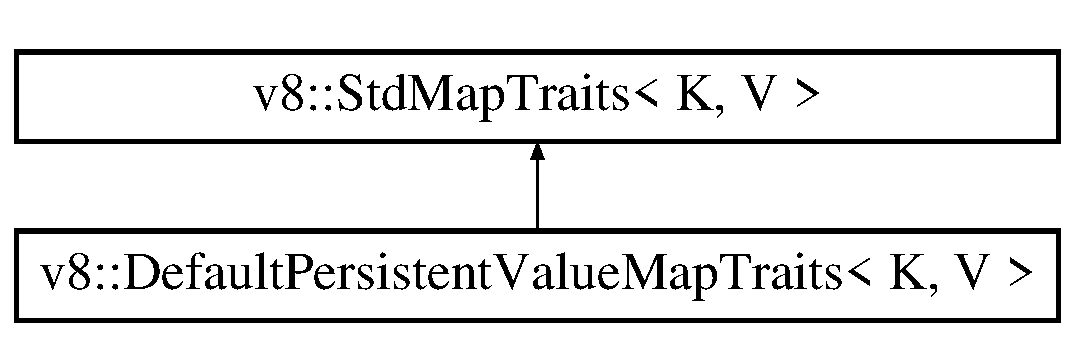
\includegraphics[height=2.000000cm]{classv8_1_1_default_persistent_value_map_traits}
\end{center}
\end{figure}
\subsection*{Public Types}
\begin{DoxyCompactItemize}
\item 
typedef \hyperlink{classv8_1_1_persistent_value_map}{Persistent\+Value\+Map}$<$ K, V, \hyperlink{classv8_1_1_default_persistent_value_map_traits}{Default\+Persistent\+Value\+Map\+Traits}$<$ K, V $>$ $>$ {\bfseries Map\+Type}\hypertarget{classv8_1_1_default_persistent_value_map_traits_a05cbd536d6bb9ba4949198351e074854}{}\label{classv8_1_1_default_persistent_value_map_traits_a05cbd536d6bb9ba4949198351e074854}

\item 
typedef void {\bfseries Weak\+Callback\+Data\+Type}\hypertarget{classv8_1_1_default_persistent_value_map_traits_a379f8c42e727a9576fb0954bb0245d8f}{}\label{classv8_1_1_default_persistent_value_map_traits_a379f8c42e727a9576fb0954bb0245d8f}

\end{DoxyCompactItemize}
\subsection*{Static Public Member Functions}
\begin{DoxyCompactItemize}
\item 
static Weak\+Callback\+Data\+Type $\ast$ {\bfseries Weak\+Callback\+Parameter} (\hyperlink{classv8_1_1_persistent_value_map}{Map\+Type} $\ast$map, const K \&key, \hyperlink{classv8_1_1_local}{Local}$<$ V $>$ value)\hypertarget{classv8_1_1_default_persistent_value_map_traits_a63b6fc80207ce6ac7d1eaa306b68768c}{}\label{classv8_1_1_default_persistent_value_map_traits_a63b6fc80207ce6ac7d1eaa306b68768c}

\item 
static \hyperlink{classv8_1_1_persistent_value_map}{Map\+Type} $\ast$ {\bfseries Map\+From\+Weak\+Callback\+Data} (const \hyperlink{classv8_1_1_weak_callback_data}{Weak\+Callback\+Data}$<$ V, Weak\+Callback\+Data\+Type $>$ \&data)\hypertarget{classv8_1_1_default_persistent_value_map_traits_a721a7a6624ffe207af1adee6d6be2fe3}{}\label{classv8_1_1_default_persistent_value_map_traits_a721a7a6624ffe207af1adee6d6be2fe3}

\item 
static K {\bfseries Key\+From\+Weak\+Callback\+Data} (const \hyperlink{classv8_1_1_weak_callback_data}{Weak\+Callback\+Data}$<$ V, Weak\+Callback\+Data\+Type $>$ \&data)\hypertarget{classv8_1_1_default_persistent_value_map_traits_ac85c6254f23d246d78a84721a80babae}{}\label{classv8_1_1_default_persistent_value_map_traits_ac85c6254f23d246d78a84721a80babae}

\item 
static void {\bfseries Dispose\+Callback\+Data} (Weak\+Callback\+Data\+Type $\ast$data)\hypertarget{classv8_1_1_default_persistent_value_map_traits_a9e5c3a4a054b13f46065adec2c44ddfe}{}\label{classv8_1_1_default_persistent_value_map_traits_a9e5c3a4a054b13f46065adec2c44ddfe}

\item 
static void {\bfseries Dispose} (\hyperlink{classv8_1_1_isolate}{Isolate} $\ast$isolate, \hyperlink{classv8_1_1_global}{Global}$<$ V $>$ value, K key)\hypertarget{classv8_1_1_default_persistent_value_map_traits_a28f1a2d349eb5a6ad376b6e968d51490}{}\label{classv8_1_1_default_persistent_value_map_traits_a28f1a2d349eb5a6ad376b6e968d51490}

\end{DoxyCompactItemize}
\subsection*{Static Public Attributes}
\begin{DoxyCompactItemize}
\item 
static const Persistent\+Container\+Callback\+Type {\bfseries k\+Callback\+Type} = k\+Not\+Weak\hypertarget{classv8_1_1_default_persistent_value_map_traits_a1f57d8246e4ace68bc9be1047eb7cc40}{}\label{classv8_1_1_default_persistent_value_map_traits_a1f57d8246e4ace68bc9be1047eb7cc40}

\end{DoxyCompactItemize}


\subsection{Detailed Description}
\subsubsection*{template$<$typename K, typename V$>$\\*
class v8\+::\+Default\+Persistent\+Value\+Map\+Traits$<$ K, V $>$}

A default trait implementation for \hyperlink{classv8_1_1_persistent_value_map}{Persistent\+Value\+Map}, which inherits a std\+:map backing map from \hyperlink{classv8_1_1_std_map_traits}{Std\+Map\+Traits} and holds non-\/weak persistent objects and has no special Dispose handling.

You should not derive from this class, since Map\+Type depends on the surrounding class, and hence a subclass cannot simply inherit the methods. 

The documentation for this class was generated from the following file\+:\begin{DoxyCompactItemize}
\item 
include/v8-\/util.\+h\end{DoxyCompactItemize}

\hypertarget{classv8_1_1_default_persistent_value_vector_traits}{}\section{v8\+:\+:Default\+Persistent\+Value\+Vector\+Traits Class Reference}
\label{classv8_1_1_default_persistent_value_vector_traits}\index{v8\+::\+Default\+Persistent\+Value\+Vector\+Traits@{v8\+::\+Default\+Persistent\+Value\+Vector\+Traits}}
\subsection*{Public Types}
\begin{DoxyCompactItemize}
\item 
typedef std\+::vector$<$ Persistent\+Container\+Value $>$ {\bfseries Impl}\hypertarget{classv8_1_1_default_persistent_value_vector_traits_ac5093f7deea6cfc8672c529be4afdef4}{}\label{classv8_1_1_default_persistent_value_vector_traits_ac5093f7deea6cfc8672c529be4afdef4}

\end{DoxyCompactItemize}
\subsection*{Static Public Member Functions}
\begin{DoxyCompactItemize}
\item 
static void {\bfseries Append} (Impl $\ast$impl, Persistent\+Container\+Value value)\hypertarget{classv8_1_1_default_persistent_value_vector_traits_ac3088f4b37e68ca9ed668a859f89cf21}{}\label{classv8_1_1_default_persistent_value_vector_traits_ac3088f4b37e68ca9ed668a859f89cf21}

\item 
static bool {\bfseries Is\+Empty} (const Impl $\ast$impl)\hypertarget{classv8_1_1_default_persistent_value_vector_traits_a5b410d98817c143d2a3bf0e9dac34bd0}{}\label{classv8_1_1_default_persistent_value_vector_traits_a5b410d98817c143d2a3bf0e9dac34bd0}

\item 
static size\+\_\+t {\bfseries Size} (const Impl $\ast$impl)\hypertarget{classv8_1_1_default_persistent_value_vector_traits_a49748bb910ea3482c078c1a8e566bd44}{}\label{classv8_1_1_default_persistent_value_vector_traits_a49748bb910ea3482c078c1a8e566bd44}

\item 
static Persistent\+Container\+Value {\bfseries Get} (const Impl $\ast$impl, size\+\_\+t i)\hypertarget{classv8_1_1_default_persistent_value_vector_traits_ab9787aa7b041a30714cd17258c886cd7}{}\label{classv8_1_1_default_persistent_value_vector_traits_ab9787aa7b041a30714cd17258c886cd7}

\item 
static void {\bfseries Reserve\+Capacity} (Impl $\ast$impl, size\+\_\+t capacity)\hypertarget{classv8_1_1_default_persistent_value_vector_traits_afda15875d9691152b30549e4dbe4eb95}{}\label{classv8_1_1_default_persistent_value_vector_traits_afda15875d9691152b30549e4dbe4eb95}

\item 
static void {\bfseries Clear} (Impl $\ast$impl)\hypertarget{classv8_1_1_default_persistent_value_vector_traits_ab15a15e95f274defd3362536ae502361}{}\label{classv8_1_1_default_persistent_value_vector_traits_ab15a15e95f274defd3362536ae502361}

\end{DoxyCompactItemize}


The documentation for this class was generated from the following file\+:\begin{DoxyCompactItemize}
\item 
/\+Users/joshgav/node/v8/include/v8-\/util.\+h\end{DoxyCompactItemize}

\hypertarget{classv8_1_1_isolate_1_1_disallow_javascript_execution_scope}{}\section{v8\+:\+:Isolate\+:\+:Disallow\+Javascript\+Execution\+Scope Class Reference}
\label{classv8_1_1_isolate_1_1_disallow_javascript_execution_scope}\index{v8\+::\+Isolate\+::\+Disallow\+Javascript\+Execution\+Scope@{v8\+::\+Isolate\+::\+Disallow\+Javascript\+Execution\+Scope}}


{\ttfamily \#include $<$v8.\+h$>$}

\subsection*{Public Types}
\begin{DoxyCompactItemize}
\item 
enum {\bfseries On\+Failure} \{ \\*
{\bfseries C\+R\+A\+S\+H\+\_\+\+O\+N\+\_\+\+F\+A\+I\+L\+U\+RE}, 
\\*
{\bfseries T\+H\+R\+O\+W\+\_\+\+O\+N\+\_\+\+F\+A\+I\+L\+U\+RE}
 \}\hypertarget{classv8_1_1_isolate_1_1_disallow_javascript_execution_scope_aeb586bef085fba34f97c09afd07ea843}{}\label{classv8_1_1_isolate_1_1_disallow_javascript_execution_scope_aeb586bef085fba34f97c09afd07ea843}

\end{DoxyCompactItemize}
\subsection*{Public Member Functions}
\begin{DoxyCompactItemize}
\item 
{\bfseries Disallow\+Javascript\+Execution\+Scope} (\hyperlink{classv8_1_1_isolate}{Isolate} $\ast$isolate, On\+Failure on\+\_\+failure)\hypertarget{classv8_1_1_isolate_1_1_disallow_javascript_execution_scope_a64813f7832ddca3014a7b98730a13948}{}\label{classv8_1_1_isolate_1_1_disallow_javascript_execution_scope_a64813f7832ddca3014a7b98730a13948}

\end{DoxyCompactItemize}
\subsection*{Private Member Functions}
\begin{DoxyCompactItemize}
\item 
{\bfseries Disallow\+Javascript\+Execution\+Scope} (const \hyperlink{classv8_1_1_isolate_1_1_disallow_javascript_execution_scope}{Disallow\+Javascript\+Execution\+Scope} \&)\hypertarget{classv8_1_1_isolate_1_1_disallow_javascript_execution_scope_a08a0a0dfb4804078bb86bf266aa36f05}{}\label{classv8_1_1_isolate_1_1_disallow_javascript_execution_scope_a08a0a0dfb4804078bb86bf266aa36f05}

\item 
\hyperlink{classv8_1_1_isolate_1_1_disallow_javascript_execution_scope}{Disallow\+Javascript\+Execution\+Scope} \& {\bfseries operator=} (const \hyperlink{classv8_1_1_isolate_1_1_disallow_javascript_execution_scope}{Disallow\+Javascript\+Execution\+Scope} \&)\hypertarget{classv8_1_1_isolate_1_1_disallow_javascript_execution_scope_aa8f45d19c0dc9467a0df64e4081ce75c}{}\label{classv8_1_1_isolate_1_1_disallow_javascript_execution_scope_aa8f45d19c0dc9467a0df64e4081ce75c}

\end{DoxyCompactItemize}
\subsection*{Private Attributes}
\begin{DoxyCompactItemize}
\item 
bool {\bfseries on\+\_\+failure\+\_\+}\hypertarget{classv8_1_1_isolate_1_1_disallow_javascript_execution_scope_a2b3fe3cb1347fadbb6233e3ba4802ed9}{}\label{classv8_1_1_isolate_1_1_disallow_javascript_execution_scope_a2b3fe3cb1347fadbb6233e3ba4802ed9}

\item 
void $\ast$ {\bfseries internal\+\_\+}\hypertarget{classv8_1_1_isolate_1_1_disallow_javascript_execution_scope_ac86111f7dadf1eb5d5ac2c49b3faa06a}{}\label{classv8_1_1_isolate_1_1_disallow_javascript_execution_scope_ac86111f7dadf1eb5d5ac2c49b3faa06a}

\end{DoxyCompactItemize}


\subsection{Detailed Description}
Assert that no Javascript code is invoked. 

The documentation for this class was generated from the following files\+:\begin{DoxyCompactItemize}
\item 
/\+Users/joshgav/node/v8/include/v8.\+h\item 
/\+Users/joshgav/node/v8/src/api.\+cc\end{DoxyCompactItemize}

\hypertarget{classv8_1_1_embedder_heap_tracer}{}\section{v8\+:\+:Embedder\+Heap\+Tracer Class Reference}
\label{classv8_1_1_embedder_heap_tracer}\index{v8\+::\+Embedder\+Heap\+Tracer@{v8\+::\+Embedder\+Heap\+Tracer}}


{\ttfamily \#include $<$v8.\+h$>$}

\subsection*{Public Member Functions}
\begin{DoxyCompactItemize}
\item 
virtual void \hyperlink{classv8_1_1_embedder_heap_tracer_af4f747aa1d77a0d2f341846b94f6b1ce}{Trace\+Prologue} ()=0
\item 
virtual void \hyperlink{classv8_1_1_embedder_heap_tracer_a94aa3bb3651e969f0f0726ee1c79cc3c}{Trace\+Wrappers\+From} (const std\+::vector$<$ std\+::pair$<$ void $\ast$, void $\ast$ $>$ $>$ \&internal\+\_\+fields)=0
\item 
virtual void \hyperlink{classv8_1_1_embedder_heap_tracer_a61b8dc3260247e2c47af8ad8f5775991}{Trace\+Epilogue} ()=0
\end{DoxyCompactItemize}


\subsection{Detailed Description}
Interface for tracing through the embedder heap. During the \hyperlink{namespacev8}{v8} garbage collection, \hyperlink{namespacev8}{v8} collects hidden fields of all potential wrappers, and at the end of its marking phase iterates the collection and asks the embedder to trace through its heap and call \hyperlink{classv8_1_1_persistent_base_a14c051e0080bbe7fbe02be35865b9923}{Persistent\+Base\+::\+Register\+External\+Reference} on each js object reachable from any of the given wrappers.

Before the first call to the Trace\+Wrappers\+From function Trace\+Prologue will be called. When the garbage collection cycle is finished, Trace\+Epilogue will be called. 

\subsection{Member Function Documentation}
\index{v8\+::\+Embedder\+Heap\+Tracer@{v8\+::\+Embedder\+Heap\+Tracer}!Trace\+Epilogue@{Trace\+Epilogue}}
\index{Trace\+Epilogue@{Trace\+Epilogue}!v8\+::\+Embedder\+Heap\+Tracer@{v8\+::\+Embedder\+Heap\+Tracer}}
\subsubsection[{\texorpdfstring{Trace\+Epilogue()=0}{TraceEpilogue()=0}}]{\setlength{\rightskip}{0pt plus 5cm}virtual void v8\+::\+Embedder\+Heap\+Tracer\+::\+Trace\+Epilogue (
\begin{DoxyParamCaption}
{}
\end{DoxyParamCaption}
)\hspace{0.3cm}{\ttfamily [pure virtual]}}\hypertarget{classv8_1_1_embedder_heap_tracer_a61b8dc3260247e2c47af8ad8f5775991}{}\label{classv8_1_1_embedder_heap_tracer_a61b8dc3260247e2c47af8ad8f5775991}
\hyperlink{classv8_1_1_v8}{V8} will call this method at the end of the gc cycle. Allocation is {\itshape not} allowed in the Trace\+Epilogue. \index{v8\+::\+Embedder\+Heap\+Tracer@{v8\+::\+Embedder\+Heap\+Tracer}!Trace\+Prologue@{Trace\+Prologue}}
\index{Trace\+Prologue@{Trace\+Prologue}!v8\+::\+Embedder\+Heap\+Tracer@{v8\+::\+Embedder\+Heap\+Tracer}}
\subsubsection[{\texorpdfstring{Trace\+Prologue()=0}{TracePrologue()=0}}]{\setlength{\rightskip}{0pt plus 5cm}virtual void v8\+::\+Embedder\+Heap\+Tracer\+::\+Trace\+Prologue (
\begin{DoxyParamCaption}
{}
\end{DoxyParamCaption}
)\hspace{0.3cm}{\ttfamily [pure virtual]}}\hypertarget{classv8_1_1_embedder_heap_tracer_af4f747aa1d77a0d2f341846b94f6b1ce}{}\label{classv8_1_1_embedder_heap_tracer_af4f747aa1d77a0d2f341846b94f6b1ce}
\hyperlink{classv8_1_1_v8}{V8} will call this method at the beginning of the gc cycle. \index{v8\+::\+Embedder\+Heap\+Tracer@{v8\+::\+Embedder\+Heap\+Tracer}!Trace\+Wrappers\+From@{Trace\+Wrappers\+From}}
\index{Trace\+Wrappers\+From@{Trace\+Wrappers\+From}!v8\+::\+Embedder\+Heap\+Tracer@{v8\+::\+Embedder\+Heap\+Tracer}}
\subsubsection[{\texorpdfstring{Trace\+Wrappers\+From(const std\+::vector$<$ std\+::pair$<$ void $\ast$, void $\ast$ $>$ $>$ \&internal\+\_\+fields)=0}{TraceWrappersFrom(const std::vector< std::pair< void *, void * > > &internal_fields)=0}}]{\setlength{\rightskip}{0pt plus 5cm}virtual void v8\+::\+Embedder\+Heap\+Tracer\+::\+Trace\+Wrappers\+From (
\begin{DoxyParamCaption}
\item[{const std\+::vector$<$ std\+::pair$<$ void $\ast$, void $\ast$ $>$ $>$ \&}]{internal\+\_\+fields}
\end{DoxyParamCaption}
)\hspace{0.3cm}{\ttfamily [pure virtual]}}\hypertarget{classv8_1_1_embedder_heap_tracer_a94aa3bb3651e969f0f0726ee1c79cc3c}{}\label{classv8_1_1_embedder_heap_tracer_a94aa3bb3651e969f0f0726ee1c79cc3c}
\hyperlink{classv8_1_1_v8}{V8} will call this method with internal fields of a potential wrappers. Embedder is expected to trace its heap (synchronously) and call \hyperlink{classv8_1_1_persistent_base_a14c051e0080bbe7fbe02be35865b9923}{Persistent\+Base\+::\+Register\+External\+Reference()} on all wrappers reachable from any of the given wrappers. 

The documentation for this class was generated from the following file\+:\begin{DoxyCompactItemize}
\item 
include/v8.\+h\end{DoxyCompactItemize}

\hypertarget{classv8_1_1_escapable_handle_scope}{}\section{v8\+:\+:Escapable\+Handle\+Scope Class Reference}
\label{classv8_1_1_escapable_handle_scope}\index{v8\+::\+Escapable\+Handle\+Scope@{v8\+::\+Escapable\+Handle\+Scope}}


{\ttfamily \#include $<$v8.\+h$>$}

Inheritance diagram for v8\+:\+:Escapable\+Handle\+Scope\+:\begin{figure}[H]
\begin{center}
\leavevmode
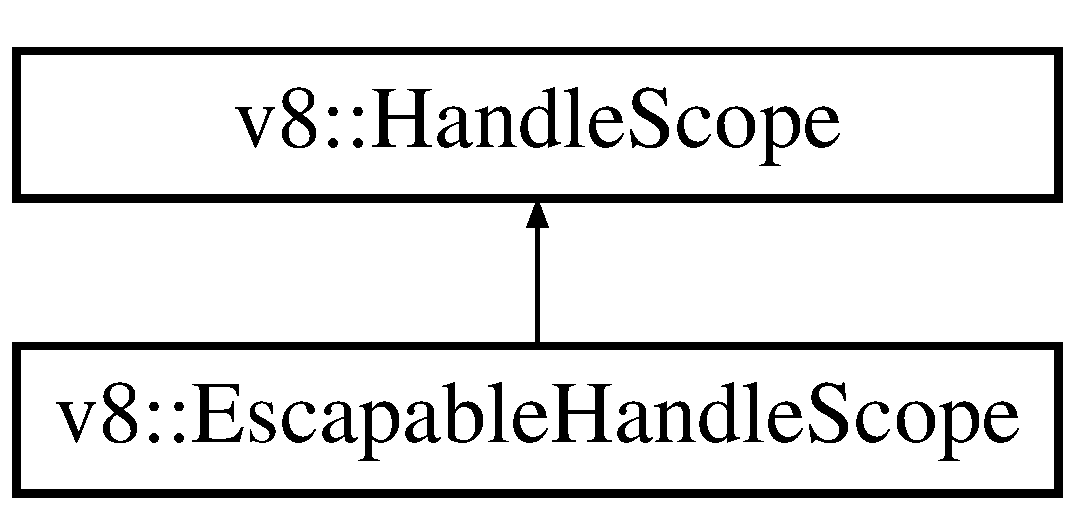
\includegraphics[height=2.000000cm]{classv8_1_1_escapable_handle_scope}
\end{center}
\end{figure}
\subsection*{Public Member Functions}
\begin{DoxyCompactItemize}
\item 
{\bfseries Escapable\+Handle\+Scope} (\hyperlink{classv8_1_1_isolate}{Isolate} $\ast$isolate)\hypertarget{classv8_1_1_escapable_handle_scope_aea39a7fd4dee6da31f3921ff891e1731}{}\label{classv8_1_1_escapable_handle_scope_aea39a7fd4dee6da31f3921ff891e1731}

\item 
{\footnotesize template$<$class T $>$ }\\V8\+\_\+\+I\+N\+L\+I\+NE \hyperlink{classv8_1_1_local}{Local}$<$ T $>$ \hyperlink{classv8_1_1_escapable_handle_scope_afdf0d3850978f65d1a827f78b3a2b6fd}{Escape} (\hyperlink{classv8_1_1_local}{Local}$<$ T $>$ value)
\end{DoxyCompactItemize}
\subsection*{Private Member Functions}
\begin{DoxyCompactItemize}
\item 
\hyperlink{classv8_1_1internal_1_1_object}{internal\+::\+Object} $\ast$$\ast$ {\bfseries Escape} (\hyperlink{classv8_1_1internal_1_1_object}{internal\+::\+Object} $\ast$$\ast$escape\+\_\+value)\hypertarget{classv8_1_1_escapable_handle_scope_a18a472064c6788f59282ceffa3df30eb}{}\label{classv8_1_1_escapable_handle_scope_a18a472064c6788f59282ceffa3df30eb}

\item 
{\bfseries Escapable\+Handle\+Scope} (const \hyperlink{classv8_1_1_escapable_handle_scope}{Escapable\+Handle\+Scope} \&)\hypertarget{classv8_1_1_escapable_handle_scope_a3e313c7cf1656a443d947303c3220931}{}\label{classv8_1_1_escapable_handle_scope_a3e313c7cf1656a443d947303c3220931}

\item 
void {\bfseries operator=} (const \hyperlink{classv8_1_1_escapable_handle_scope}{Escapable\+Handle\+Scope} \&)\hypertarget{classv8_1_1_escapable_handle_scope_a3fbf3f11d4089d8a730d4171bf8f1bed}{}\label{classv8_1_1_escapable_handle_scope_a3fbf3f11d4089d8a730d4171bf8f1bed}

\item 
void $\ast$ {\bfseries operator new} (size\+\_\+t size)\hypertarget{classv8_1_1_escapable_handle_scope_adf445b7a17fe29a93c9524fe72b65b28}{}\label{classv8_1_1_escapable_handle_scope_adf445b7a17fe29a93c9524fe72b65b28}

\item 
void {\bfseries operator delete} (void $\ast$, size\+\_\+t)\hypertarget{classv8_1_1_escapable_handle_scope_a082688365df2e134a510dd3bc67629af}{}\label{classv8_1_1_escapable_handle_scope_a082688365df2e134a510dd3bc67629af}

\end{DoxyCompactItemize}
\subsection*{Private Attributes}
\begin{DoxyCompactItemize}
\item 
\hyperlink{classv8_1_1internal_1_1_object}{internal\+::\+Object} $\ast$$\ast$ {\bfseries escape\+\_\+slot\+\_\+}\hypertarget{classv8_1_1_escapable_handle_scope_aa452d2cad22ccec2675174e01526d025}{}\label{classv8_1_1_escapable_handle_scope_aa452d2cad22ccec2675174e01526d025}

\end{DoxyCompactItemize}
\subsection*{Additional Inherited Members}


\subsection{Detailed Description}
A \hyperlink{classv8_1_1_handle_scope}{Handle\+Scope} which first allocates a handle in the current scope which will be later filled with the escape value. 

\subsection{Member Function Documentation}
\index{v8\+::\+Escapable\+Handle\+Scope@{v8\+::\+Escapable\+Handle\+Scope}!Escape@{Escape}}
\index{Escape@{Escape}!v8\+::\+Escapable\+Handle\+Scope@{v8\+::\+Escapable\+Handle\+Scope}}
\subsubsection[{\texorpdfstring{Escape(\+Local$<$ T $>$ value)}{Escape(Local< T > value)}}]{\setlength{\rightskip}{0pt plus 5cm}template$<$class T $>$ V8\+\_\+\+I\+N\+L\+I\+NE {\bf Local}$<$T$>$ v8\+::\+Escapable\+Handle\+Scope\+::\+Escape (
\begin{DoxyParamCaption}
\item[{{\bf Local}$<$ T $>$}]{value}
\end{DoxyParamCaption}
)\hspace{0.3cm}{\ttfamily [inline]}}\hypertarget{classv8_1_1_escapable_handle_scope_afdf0d3850978f65d1a827f78b3a2b6fd}{}\label{classv8_1_1_escapable_handle_scope_afdf0d3850978f65d1a827f78b3a2b6fd}
Pushes the value into the previous scope and returns a handle to it. Cannot be called twice. 

The documentation for this class was generated from the following files\+:\begin{DoxyCompactItemize}
\item 
/\+Users/joshgav/node/v8/include/v8.\+h\item 
/\+Users/joshgav/node/v8/src/api.\+cc\end{DoxyCompactItemize}

\hypertarget{classv8_1_1_eternal}{}\section{v8\+:\+:Eternal$<$ T $>$ Class Template Reference}
\label{classv8_1_1_eternal}\index{v8\+::\+Eternal$<$ T $>$@{v8\+::\+Eternal$<$ T $>$}}
\subsection*{Public Member Functions}
\begin{DoxyCompactItemize}
\item 
{\footnotesize template$<$class S $>$ }\\V8\+\_\+\+I\+N\+L\+I\+NE {\bfseries Eternal} (\hyperlink{classv8_1_1_isolate}{Isolate} $\ast$isolate, \hyperlink{classv8_1_1_local}{Local}$<$ S $>$ handle)\hypertarget{classv8_1_1_eternal_ad7522d8b51e072dcbc4261bc1f155bcb}{}\label{classv8_1_1_eternal_ad7522d8b51e072dcbc4261bc1f155bcb}

\item 
V8\+\_\+\+I\+N\+L\+I\+NE \hyperlink{classv8_1_1_local}{Local}$<$ T $>$ {\bfseries Get} (\hyperlink{classv8_1_1_isolate}{Isolate} $\ast$isolate)\hypertarget{classv8_1_1_eternal_ae9614309d9c93fe484d81926e31ed6b7}{}\label{classv8_1_1_eternal_ae9614309d9c93fe484d81926e31ed6b7}

\item 
V8\+\_\+\+I\+N\+L\+I\+NE bool {\bfseries Is\+Empty} ()\hypertarget{classv8_1_1_eternal_a5d77cbfe0662af5fe75172be9a8f1d5d}{}\label{classv8_1_1_eternal_a5d77cbfe0662af5fe75172be9a8f1d5d}

\item 
{\footnotesize template$<$class S $>$ }\\V8\+\_\+\+I\+N\+L\+I\+NE void {\bfseries Set} (\hyperlink{classv8_1_1_isolate}{Isolate} $\ast$isolate, \hyperlink{classv8_1_1_local}{Local}$<$ S $>$ handle)\hypertarget{classv8_1_1_eternal_a75a32f5c428a0d47e13f66dbdeb9adba}{}\label{classv8_1_1_eternal_a75a32f5c428a0d47e13f66dbdeb9adba}

\item 
{\footnotesize template$<$class S $>$ }\\void {\bfseries Set} (\hyperlink{classv8_1_1_isolate}{Isolate} $\ast$isolate, \hyperlink{classv8_1_1_local}{Local}$<$ S $>$ handle)\hypertarget{classv8_1_1_eternal_a2f9dcec02b2c2f7d4b55aee0d8b9881a}{}\label{classv8_1_1_eternal_a2f9dcec02b2c2f7d4b55aee0d8b9881a}

\end{DoxyCompactItemize}
\subsection*{Private Attributes}
\begin{DoxyCompactItemize}
\item 
int {\bfseries index\+\_\+}\hypertarget{classv8_1_1_eternal_ad186efc74d3640ebef961abc1f7430cf}{}\label{classv8_1_1_eternal_ad186efc74d3640ebef961abc1f7430cf}

\end{DoxyCompactItemize}
\subsection*{Static Private Attributes}
\begin{DoxyCompactItemize}
\item 
static const int {\bfseries k\+Initial\+Value} = -\/1\hypertarget{classv8_1_1_eternal_adfc0b4ef32d5926b58b0b216eb051298}{}\label{classv8_1_1_eternal_adfc0b4ef32d5926b58b0b216eb051298}

\end{DoxyCompactItemize}


The documentation for this class was generated from the following file\+:\begin{DoxyCompactItemize}
\item 
include/v8.\+h\end{DoxyCompactItemize}

\hypertarget{classv8_1_1_debug_1_1_event_details}{}\section{v8\+:\+:Debug\+:\+:Event\+Details Class Reference}
\label{classv8_1_1_debug_1_1_event_details}\index{v8\+::\+Debug\+::\+Event\+Details@{v8\+::\+Debug\+::\+Event\+Details}}


{\ttfamily \#include $<$v8-\/debug.\+h$>$}

Inheritance diagram for v8\+:\+:Debug\+:\+:Event\+Details\+:\begin{figure}[H]
\begin{center}
\leavevmode
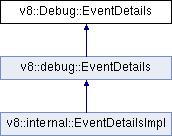
\includegraphics[height=2.000000cm]{classv8_1_1_debug_1_1_event_details}
\end{center}
\end{figure}
\subsection*{Public Member Functions}
\begin{DoxyCompactItemize}
\item 
virtual Debug\+Event \hyperlink{classv8_1_1_debug_1_1_event_details_a3743044e92847f4647cef5f597ac1863}{Get\+Event} () const  =0
\item 
virtual \hyperlink{classv8_1_1_local}{Local}$<$ \hyperlink{classv8_1_1_object}{Object} $>$ \hyperlink{classv8_1_1_debug_1_1_event_details_a0d68512e6225f318b87e9ec440282f73}{Get\+Execution\+State} () const  =0
\item 
virtual \hyperlink{classv8_1_1_local}{Local}$<$ \hyperlink{classv8_1_1_object}{Object} $>$ {\bfseries Get\+Event\+Data} () const  =0\hypertarget{classv8_1_1_debug_1_1_event_details_aa1bb2a9db9466badb797067a5cdbd466}{}\label{classv8_1_1_debug_1_1_event_details_aa1bb2a9db9466badb797067a5cdbd466}

\item 
virtual \hyperlink{classv8_1_1_local}{Local}$<$ \hyperlink{classv8_1_1_context}{Context} $>$ \hyperlink{classv8_1_1_debug_1_1_event_details_a31863285c87e36f5c744e148cc3650e5}{Get\+Event\+Context} () const  =0
\item 
virtual \hyperlink{classv8_1_1_local}{Local}$<$ \hyperlink{classv8_1_1_value}{Value} $>$ \hyperlink{classv8_1_1_debug_1_1_event_details_acad01eae9062893a7d5252a0596ebb3d}{Get\+Callback\+Data} () const  =0
\item 
virtual \hyperlink{classv8_1_1_debug_1_1_client_data}{Client\+Data} $\ast$ \hyperlink{classv8_1_1_debug_1_1_event_details_ac9d8db55000c0fd27b1a02cbef5b267b}{Get\+Client\+Data} () const  =0
\end{DoxyCompactItemize}


\subsection{Detailed Description}
An event details object passed to the debug event listener. 

\subsection{Member Function Documentation}
\index{v8\+::\+Debug\+::\+Event\+Details@{v8\+::\+Debug\+::\+Event\+Details}!Get\+Callback\+Data@{Get\+Callback\+Data}}
\index{Get\+Callback\+Data@{Get\+Callback\+Data}!v8\+::\+Debug\+::\+Event\+Details@{v8\+::\+Debug\+::\+Event\+Details}}
\subsubsection[{\texorpdfstring{Get\+Callback\+Data() const  =0}{GetCallbackData() const  =0}}]{\setlength{\rightskip}{0pt plus 5cm}virtual {\bf Local}$<${\bf Value}$>$ v8\+::\+Debug\+::\+Event\+Details\+::\+Get\+Callback\+Data (
\begin{DoxyParamCaption}
{}
\end{DoxyParamCaption}
) const\hspace{0.3cm}{\ttfamily [pure virtual]}}\hypertarget{classv8_1_1_debug_1_1_event_details_acad01eae9062893a7d5252a0596ebb3d}{}\label{classv8_1_1_debug_1_1_event_details_acad01eae9062893a7d5252a0596ebb3d}
Client data passed with the corresponding callback when it was registered. 

Implemented in \hyperlink{classv8_1_1internal_1_1_event_details_impl_a34b2e3cdc3ef2ad14761b85af5ef174b}{v8\+::internal\+::\+Event\+Details\+Impl}.

\index{v8\+::\+Debug\+::\+Event\+Details@{v8\+::\+Debug\+::\+Event\+Details}!Get\+Client\+Data@{Get\+Client\+Data}}
\index{Get\+Client\+Data@{Get\+Client\+Data}!v8\+::\+Debug\+::\+Event\+Details@{v8\+::\+Debug\+::\+Event\+Details}}
\subsubsection[{\texorpdfstring{Get\+Client\+Data() const  =0}{GetClientData() const  =0}}]{\setlength{\rightskip}{0pt plus 5cm}virtual {\bf Client\+Data}$\ast$ v8\+::\+Debug\+::\+Event\+Details\+::\+Get\+Client\+Data (
\begin{DoxyParamCaption}
{}
\end{DoxyParamCaption}
) const\hspace{0.3cm}{\ttfamily [pure virtual]}}\hypertarget{classv8_1_1_debug_1_1_event_details_ac9d8db55000c0fd27b1a02cbef5b267b}{}\label{classv8_1_1_debug_1_1_event_details_ac9d8db55000c0fd27b1a02cbef5b267b}
Client data passed to Debug\+Break\+For\+Command function. The debugger takes ownership of the data and will delete it even if there is no message handler. 

Implemented in \hyperlink{classv8_1_1internal_1_1_event_details_impl_a562a0107f0d37a400eaf92031d829218}{v8\+::internal\+::\+Event\+Details\+Impl}.

\index{v8\+::\+Debug\+::\+Event\+Details@{v8\+::\+Debug\+::\+Event\+Details}!Get\+Event@{Get\+Event}}
\index{Get\+Event@{Get\+Event}!v8\+::\+Debug\+::\+Event\+Details@{v8\+::\+Debug\+::\+Event\+Details}}
\subsubsection[{\texorpdfstring{Get\+Event() const  =0}{GetEvent() const  =0}}]{\setlength{\rightskip}{0pt plus 5cm}virtual Debug\+Event v8\+::\+Debug\+::\+Event\+Details\+::\+Get\+Event (
\begin{DoxyParamCaption}
{}
\end{DoxyParamCaption}
) const\hspace{0.3cm}{\ttfamily [pure virtual]}}\hypertarget{classv8_1_1_debug_1_1_event_details_a3743044e92847f4647cef5f597ac1863}{}\label{classv8_1_1_debug_1_1_event_details_a3743044e92847f4647cef5f597ac1863}
Event type. 

Implemented in \hyperlink{classv8_1_1internal_1_1_event_details_impl_a135085e7265cc9932ad6065649d6ffef}{v8\+::internal\+::\+Event\+Details\+Impl}.

\index{v8\+::\+Debug\+::\+Event\+Details@{v8\+::\+Debug\+::\+Event\+Details}!Get\+Event\+Context@{Get\+Event\+Context}}
\index{Get\+Event\+Context@{Get\+Event\+Context}!v8\+::\+Debug\+::\+Event\+Details@{v8\+::\+Debug\+::\+Event\+Details}}
\subsubsection[{\texorpdfstring{Get\+Event\+Context() const  =0}{GetEventContext() const  =0}}]{\setlength{\rightskip}{0pt plus 5cm}virtual {\bf Local}$<${\bf Context}$>$ v8\+::\+Debug\+::\+Event\+Details\+::\+Get\+Event\+Context (
\begin{DoxyParamCaption}
{}
\end{DoxyParamCaption}
) const\hspace{0.3cm}{\ttfamily [pure virtual]}}\hypertarget{classv8_1_1_debug_1_1_event_details_a31863285c87e36f5c744e148cc3650e5}{}\label{classv8_1_1_debug_1_1_event_details_a31863285c87e36f5c744e148cc3650e5}
Get the context active when the debug event happened. Note this is not the current active context as the Java\+Script part of the debugger is running in its own context which is entered at this point. 

Implemented in \hyperlink{classv8_1_1internal_1_1_event_details_impl_a3125bc51e53d62ab3dc967cb16a4eedb}{v8\+::internal\+::\+Event\+Details\+Impl}.

\index{v8\+::\+Debug\+::\+Event\+Details@{v8\+::\+Debug\+::\+Event\+Details}!Get\+Execution\+State@{Get\+Execution\+State}}
\index{Get\+Execution\+State@{Get\+Execution\+State}!v8\+::\+Debug\+::\+Event\+Details@{v8\+::\+Debug\+::\+Event\+Details}}
\subsubsection[{\texorpdfstring{Get\+Execution\+State() const  =0}{GetExecutionState() const  =0}}]{\setlength{\rightskip}{0pt plus 5cm}virtual {\bf Local}$<${\bf Object}$>$ v8\+::\+Debug\+::\+Event\+Details\+::\+Get\+Execution\+State (
\begin{DoxyParamCaption}
{}
\end{DoxyParamCaption}
) const\hspace{0.3cm}{\ttfamily [pure virtual]}}\hypertarget{classv8_1_1_debug_1_1_event_details_a0d68512e6225f318b87e9ec440282f73}{}\label{classv8_1_1_debug_1_1_event_details_a0d68512e6225f318b87e9ec440282f73}
Access to execution state and event data of the debug event. Don\textquotesingle{}t store these cross callbacks as their content becomes invalid. 

Implemented in \hyperlink{classv8_1_1internal_1_1_event_details_impl_ad58648fb347ec33930390d78a54d9def}{v8\+::internal\+::\+Event\+Details\+Impl}.



The documentation for this class was generated from the following file\+:\begin{DoxyCompactItemize}
\item 
/\+Users/joshgav/node/v8/include/v8-\/debug.\+h\end{DoxyCompactItemize}

\hypertarget{classv8_1_1_exception}{}\section{v8\+:\+:Exception Class Reference}
\label{classv8_1_1_exception}\index{v8\+::\+Exception@{v8\+::\+Exception}}


{\ttfamily \#include $<$v8.\+h$>$}

\subsection*{Public Member Functions}
\begin{DoxyCompactItemize}
\item 
{\bfseries V8\+\_\+\+D\+E\+P\+R\+E\+C\+A\+T\+ED} (\char`\"{}Use version with an \hyperlink{classv8_1_1_isolate}{Isolate}$\ast$\char`\"{}, static \hyperlink{classv8_1_1_local}{Local}$<$ \hyperlink{classv8_1_1_message}{Message} $>$ \hyperlink{classv8_1_1_exception_a8d575a721cf0fd5b325afb8b586c0d1e}{Create\+Message}(\hyperlink{classv8_1_1_local}{Local}$<$ \hyperlink{classv8_1_1_value}{Value} $>$ exception))\hypertarget{classv8_1_1_exception_ae66baf48c3f461b919e66c3bb9094e64}{}\label{classv8_1_1_exception_ae66baf48c3f461b919e66c3bb9094e64}

\end{DoxyCompactItemize}
\subsection*{Static Public Member Functions}
\begin{DoxyCompactItemize}
\item 
static \hyperlink{classv8_1_1_local}{Local}$<$ \hyperlink{classv8_1_1_value}{Value} $>$ {\bfseries Range\+Error} (\hyperlink{classv8_1_1_local}{Local}$<$ \hyperlink{classv8_1_1_string}{String} $>$ message)\hypertarget{classv8_1_1_exception_a7fff335c54b4a267b5edab00ca049294}{}\label{classv8_1_1_exception_a7fff335c54b4a267b5edab00ca049294}

\item 
static \hyperlink{classv8_1_1_local}{Local}$<$ \hyperlink{classv8_1_1_value}{Value} $>$ {\bfseries Reference\+Error} (\hyperlink{classv8_1_1_local}{Local}$<$ \hyperlink{classv8_1_1_string}{String} $>$ message)\hypertarget{classv8_1_1_exception_aa9a1b1806c6ec13e0e8852a05e83f8ef}{}\label{classv8_1_1_exception_aa9a1b1806c6ec13e0e8852a05e83f8ef}

\item 
static \hyperlink{classv8_1_1_local}{Local}$<$ \hyperlink{classv8_1_1_value}{Value} $>$ {\bfseries Syntax\+Error} (\hyperlink{classv8_1_1_local}{Local}$<$ \hyperlink{classv8_1_1_string}{String} $>$ message)\hypertarget{classv8_1_1_exception_ae9efc01a15b3ea6ed0761ce4b2cfa4ab}{}\label{classv8_1_1_exception_ae9efc01a15b3ea6ed0761ce4b2cfa4ab}

\item 
static \hyperlink{classv8_1_1_local}{Local}$<$ \hyperlink{classv8_1_1_value}{Value} $>$ {\bfseries Type\+Error} (\hyperlink{classv8_1_1_local}{Local}$<$ \hyperlink{classv8_1_1_string}{String} $>$ message)\hypertarget{classv8_1_1_exception_ad06cda3370edb5b39a5c671bba28754d}{}\label{classv8_1_1_exception_ad06cda3370edb5b39a5c671bba28754d}

\item 
static \hyperlink{classv8_1_1_local}{Local}$<$ \hyperlink{classv8_1_1_value}{Value} $>$ {\bfseries Error} (\hyperlink{classv8_1_1_local}{Local}$<$ \hyperlink{classv8_1_1_string}{String} $>$ message)\hypertarget{classv8_1_1_exception_a77c6ab659f67df0cb0aa0f7c6698f019}{}\label{classv8_1_1_exception_a77c6ab659f67df0cb0aa0f7c6698f019}

\item 
static \hyperlink{classv8_1_1_local}{Local}$<$ \hyperlink{classv8_1_1_message}{Message} $>$ \hyperlink{classv8_1_1_exception_a8d575a721cf0fd5b325afb8b586c0d1e}{Create\+Message} (\hyperlink{classv8_1_1_isolate}{Isolate} $\ast$isolate, \hyperlink{classv8_1_1_local}{Local}$<$ \hyperlink{classv8_1_1_value}{Value} $>$ exception)
\item 
static \hyperlink{classv8_1_1_local}{Local}$<$ \hyperlink{classv8_1_1_stack_trace}{Stack\+Trace} $>$ \hyperlink{classv8_1_1_exception_a81d1fd3c8d729e9a8d830bc2830bfe77}{Get\+Stack\+Trace} (\hyperlink{classv8_1_1_local}{Local}$<$ \hyperlink{classv8_1_1_value}{Value} $>$ exception)
\end{DoxyCompactItemize}


\subsection{Detailed Description}
Create new error objects by calling the corresponding error object constructor with the message. 

\subsection{Member Function Documentation}
\index{v8\+::\+Exception@{v8\+::\+Exception}!Create\+Message@{Create\+Message}}
\index{Create\+Message@{Create\+Message}!v8\+::\+Exception@{v8\+::\+Exception}}
\subsubsection[{\texorpdfstring{Create\+Message(\+Isolate $\ast$isolate, Local$<$ Value $>$ exception)}{CreateMessage(Isolate *isolate, Local< Value > exception)}}]{\setlength{\rightskip}{0pt plus 5cm}static {\bf Local}$<${\bf Message}$>$ v8\+::\+Exception\+::\+Create\+Message (
\begin{DoxyParamCaption}
\item[{{\bf Isolate} $\ast$}]{isolate, }
\item[{{\bf Local}$<$ {\bf Value} $>$}]{exception}
\end{DoxyParamCaption}
)\hspace{0.3cm}{\ttfamily [static]}}\hypertarget{classv8_1_1_exception_a8d575a721cf0fd5b325afb8b586c0d1e}{}\label{classv8_1_1_exception_a8d575a721cf0fd5b325afb8b586c0d1e}
Creates an error message for the given exception. Will try to reconstruct the original stack trace from the exception value, or capture the current stack trace if not available. \index{v8\+::\+Exception@{v8\+::\+Exception}!Get\+Stack\+Trace@{Get\+Stack\+Trace}}
\index{Get\+Stack\+Trace@{Get\+Stack\+Trace}!v8\+::\+Exception@{v8\+::\+Exception}}
\subsubsection[{\texorpdfstring{Get\+Stack\+Trace(\+Local$<$ Value $>$ exception)}{GetStackTrace(Local< Value > exception)}}]{\setlength{\rightskip}{0pt plus 5cm}static {\bf Local}$<${\bf Stack\+Trace}$>$ v8\+::\+Exception\+::\+Get\+Stack\+Trace (
\begin{DoxyParamCaption}
\item[{{\bf Local}$<$ {\bf Value} $>$}]{exception}
\end{DoxyParamCaption}
)\hspace{0.3cm}{\ttfamily [static]}}\hypertarget{classv8_1_1_exception_a81d1fd3c8d729e9a8d830bc2830bfe77}{}\label{classv8_1_1_exception_a81d1fd3c8d729e9a8d830bc2830bfe77}
Returns the original stack trace that was captured at the creation time of a given exception, or an empty handle if not available. 

The documentation for this class was generated from the following file\+:\begin{DoxyCompactItemize}
\item 
include/v8.\+h\end{DoxyCompactItemize}

\hypertarget{classv8_1_1_extension}{}\section{v8\+:\+:Extension Class Reference}
\label{classv8_1_1_extension}\index{v8\+::\+Extension@{v8\+::\+Extension}}


{\ttfamily \#include $<$v8.\+h$>$}

\subsection*{Public Member Functions}
\begin{DoxyCompactItemize}
\item 
{\bfseries Extension} (const char $\ast$name, const char $\ast$source=0, int dep\+\_\+count=0, const char $\ast$$\ast$deps=0, int source\+\_\+length=-\/1)\hypertarget{classv8_1_1_extension_a10868673b7801cc1139ca3bc09bcfcf6}{}\label{classv8_1_1_extension_a10868673b7801cc1139ca3bc09bcfcf6}

\item 
virtual \hyperlink{classv8_1_1_local}{v8\+::\+Local}$<$ \hyperlink{classv8_1_1_function_template}{v8\+::\+Function\+Template} $>$ {\bfseries Get\+Native\+Function\+Template} (\hyperlink{classv8_1_1_isolate}{v8\+::\+Isolate} $\ast$isolate, \hyperlink{classv8_1_1_local}{v8\+::\+Local}$<$ \hyperlink{classv8_1_1_string}{v8\+::\+String} $>$ name)\hypertarget{classv8_1_1_extension_a39b4273aa4c7258b65bad3e1e469e59e}{}\label{classv8_1_1_extension_a39b4273aa4c7258b65bad3e1e469e59e}

\item 
const char $\ast$ {\bfseries name} () const \hypertarget{classv8_1_1_extension_a183946edbf28789f7cddecdad2d26f96}{}\label{classv8_1_1_extension_a183946edbf28789f7cddecdad2d26f96}

\item 
size\+\_\+t {\bfseries source\+\_\+length} () const \hypertarget{classv8_1_1_extension_a91da6067f79c5c354aa3184ed0746966}{}\label{classv8_1_1_extension_a91da6067f79c5c354aa3184ed0746966}

\item 
const \hyperlink{classv8_1_1_string_1_1_external_one_byte_string_resource}{String\+::\+External\+One\+Byte\+String\+Resource} $\ast$ {\bfseries source} () const \hypertarget{classv8_1_1_extension_a5c68ba79f0cf009a1c3e972d7b3b1f50}{}\label{classv8_1_1_extension_a5c68ba79f0cf009a1c3e972d7b3b1f50}

\item 
int {\bfseries dependency\+\_\+count} ()\hypertarget{classv8_1_1_extension_a7623b08e3bc42d903bd923a00317b7f9}{}\label{classv8_1_1_extension_a7623b08e3bc42d903bd923a00317b7f9}

\item 
const char $\ast$$\ast$ {\bfseries dependencies} ()\hypertarget{classv8_1_1_extension_adbec8a811d5a4554678da4a5d55dda6d}{}\label{classv8_1_1_extension_adbec8a811d5a4554678da4a5d55dda6d}

\item 
void {\bfseries set\+\_\+auto\+\_\+enable} (bool value)\hypertarget{classv8_1_1_extension_af5b752ba211315b6e9dac5c0e6e638e8}{}\label{classv8_1_1_extension_af5b752ba211315b6e9dac5c0e6e638e8}

\item 
bool {\bfseries auto\+\_\+enable} ()\hypertarget{classv8_1_1_extension_aee87ef4f9c3d7880fc3b28765d28e516}{}\label{classv8_1_1_extension_aee87ef4f9c3d7880fc3b28765d28e516}

\end{DoxyCompactItemize}
\subsection*{Private Member Functions}
\begin{DoxyCompactItemize}
\item 
{\bfseries Extension} (const \hyperlink{classv8_1_1_extension}{Extension} \&)\hypertarget{classv8_1_1_extension_a27b882e3455c86303822c8012420a5b2}{}\label{classv8_1_1_extension_a27b882e3455c86303822c8012420a5b2}

\item 
void {\bfseries operator=} (const \hyperlink{classv8_1_1_extension}{Extension} \&)\hypertarget{classv8_1_1_extension_a648d5a0b99a45a0b0554301ab697e81c}{}\label{classv8_1_1_extension_a648d5a0b99a45a0b0554301ab697e81c}

\end{DoxyCompactItemize}
\subsection*{Private Attributes}
\begin{DoxyCompactItemize}
\item 
const char $\ast$ {\bfseries name\+\_\+}\hypertarget{classv8_1_1_extension_adcdd12a726668185217ad5623e6c5a43}{}\label{classv8_1_1_extension_adcdd12a726668185217ad5623e6c5a43}

\item 
size\+\_\+t {\bfseries source\+\_\+length\+\_\+}\hypertarget{classv8_1_1_extension_a7912969d063d4efe694e0450f6ecd8bc}{}\label{classv8_1_1_extension_a7912969d063d4efe694e0450f6ecd8bc}

\item 
\hyperlink{classv8_1_1_external_one_byte_string_resource_impl}{External\+One\+Byte\+String\+Resource\+Impl} {\bfseries source\+\_\+}\hypertarget{classv8_1_1_extension_ac9242897191bf63ad580715c8469d59b}{}\label{classv8_1_1_extension_ac9242897191bf63ad580715c8469d59b}

\item 
int {\bfseries dep\+\_\+count\+\_\+}\hypertarget{classv8_1_1_extension_ac892d429dd433624cfa4c865613465f5}{}\label{classv8_1_1_extension_ac892d429dd433624cfa4c865613465f5}

\item 
const char $\ast$$\ast$ {\bfseries deps\+\_\+}\hypertarget{classv8_1_1_extension_ae8198584f50edab2521b9344fa3d443f}{}\label{classv8_1_1_extension_ae8198584f50edab2521b9344fa3d443f}

\item 
bool {\bfseries auto\+\_\+enable\+\_\+}\hypertarget{classv8_1_1_extension_a4c7d7140358ffe5c661581af0238ea62}{}\label{classv8_1_1_extension_a4c7d7140358ffe5c661581af0238ea62}

\end{DoxyCompactItemize}


\subsection{Detailed Description}
Ignore 

The documentation for this class was generated from the following file\+:\begin{DoxyCompactItemize}
\item 
include/v8.\+h\end{DoxyCompactItemize}

\hypertarget{classv8_1_1_extension_configuration}{}\section{v8\+:\+:Extension\+Configuration Class Reference}
\label{classv8_1_1_extension_configuration}\index{v8\+::\+Extension\+Configuration@{v8\+::\+Extension\+Configuration}}


{\ttfamily \#include $<$v8.\+h$>$}

\subsection*{Public Member Functions}
\begin{DoxyCompactItemize}
\item 
{\bfseries Extension\+Configuration} (int name\+\_\+count, const char $\ast$names\mbox{[}$\,$\mbox{]})\hypertarget{classv8_1_1_extension_configuration_a1189e46efe963db4aa7340cc767f276a}{}\label{classv8_1_1_extension_configuration_a1189e46efe963db4aa7340cc767f276a}

\item 
const char $\ast$$\ast$ {\bfseries begin} () const \hypertarget{classv8_1_1_extension_configuration_ae776fbc067a257bac854d9bcc9b72141}{}\label{classv8_1_1_extension_configuration_ae776fbc067a257bac854d9bcc9b72141}

\item 
const char $\ast$$\ast$ {\bfseries end} () const \hypertarget{classv8_1_1_extension_configuration_abcbebcc4782016f58fc60de82f59f61a}{}\label{classv8_1_1_extension_configuration_abcbebcc4782016f58fc60de82f59f61a}

\end{DoxyCompactItemize}
\subsection*{Private Attributes}
\begin{DoxyCompactItemize}
\item 
const int {\bfseries name\+\_\+count\+\_\+}\hypertarget{classv8_1_1_extension_configuration_a5cc34723570b88ea2bf3b00fae81d3cb}{}\label{classv8_1_1_extension_configuration_a5cc34723570b88ea2bf3b00fae81d3cb}

\item 
const char $\ast$$\ast$ {\bfseries names\+\_\+}\hypertarget{classv8_1_1_extension_configuration_a866e52fd6511b7dc86a0861dca114c90}{}\label{classv8_1_1_extension_configuration_a866e52fd6511b7dc86a0861dca114c90}

\end{DoxyCompactItemize}


\subsection{Detailed Description}
A container for extension names. 

The documentation for this class was generated from the following file\+:\begin{DoxyCompactItemize}
\item 
include/v8.\+h\end{DoxyCompactItemize}

\hypertarget{classv8_1_1_external}{}\section{v8\+:\+:External Class Reference}
\label{classv8_1_1_external}\index{v8\+::\+External@{v8\+::\+External}}


{\ttfamily \#include $<$v8.\+h$>$}

Inheritance diagram for v8\+:\+:External\+:\begin{figure}[H]
\begin{center}
\leavevmode
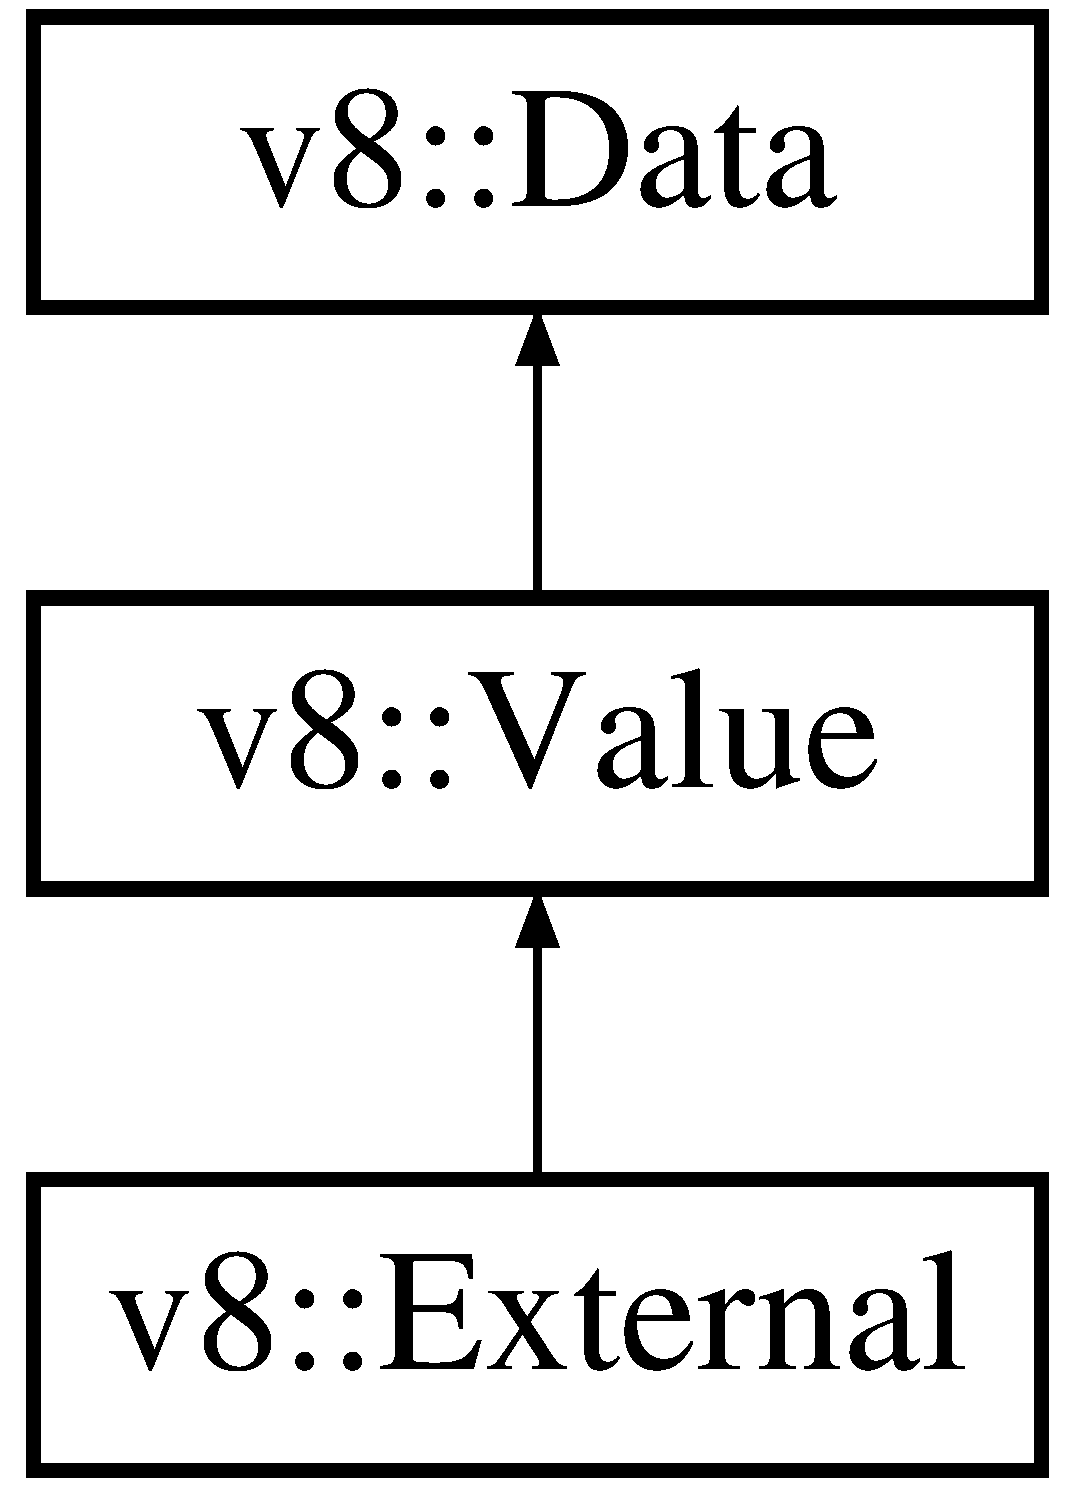
\includegraphics[height=3.000000cm]{classv8_1_1_external}
\end{center}
\end{figure}
\subsection*{Public Member Functions}
\begin{DoxyCompactItemize}
\item 
void $\ast$ {\bfseries Value} () const \hypertarget{classv8_1_1_external_ac2733ee14b5b26f369e5a335c0fe3301}{}\label{classv8_1_1_external_ac2733ee14b5b26f369e5a335c0fe3301}

\end{DoxyCompactItemize}
\subsection*{Static Public Member Functions}
\begin{DoxyCompactItemize}
\item 
static \hyperlink{classv8_1_1_local}{Local}$<$ \hyperlink{classv8_1_1_external}{External} $>$ {\bfseries New} (\hyperlink{classv8_1_1_isolate}{Isolate} $\ast$isolate, void $\ast$value)\hypertarget{classv8_1_1_external_a1e877f692e95f13ac3102707ce8cbab9}{}\label{classv8_1_1_external_a1e877f692e95f13ac3102707ce8cbab9}

\item 
static V8\+\_\+\+I\+N\+L\+I\+NE \hyperlink{classv8_1_1_external}{External} $\ast$ {\bfseries Cast} (\hyperlink{classv8_1_1_value}{Value} $\ast$obj)\hypertarget{classv8_1_1_external_a4711aba26710c5dd72f11cb81808f9c2}{}\label{classv8_1_1_external_a4711aba26710c5dd72f11cb81808f9c2}

\end{DoxyCompactItemize}
\subsection*{Static Private Member Functions}
\begin{DoxyCompactItemize}
\item 
static void {\bfseries Check\+Cast} (\hyperlink{classv8_1_1_value}{v8\+::\+Value} $\ast$obj)\hypertarget{classv8_1_1_external_a7b48d794bfa03ee712090a13dbe885ab}{}\label{classv8_1_1_external_a7b48d794bfa03ee712090a13dbe885ab}

\end{DoxyCompactItemize}


\subsection{Detailed Description}
A Java\+Script value that wraps a C++ void$\ast$. This type of value is mainly used to associate C++ data structures with Java\+Script objects. 

The documentation for this class was generated from the following file\+:\begin{DoxyCompactItemize}
\item 
/\+Users/joshgav/node/v8/include/v8.\+h\end{DoxyCompactItemize}

\hypertarget{classv8_1_1_string_1_1_external_one_byte_string_resource}{}\section{v8\+:\+:String\+:\+:External\+One\+Byte\+String\+Resource Class Reference}
\label{classv8_1_1_string_1_1_external_one_byte_string_resource}\index{v8\+::\+String\+::\+External\+One\+Byte\+String\+Resource@{v8\+::\+String\+::\+External\+One\+Byte\+String\+Resource}}


{\ttfamily \#include $<$v8.\+h$>$}

Inheritance diagram for v8\+:\+:String\+:\+:External\+One\+Byte\+String\+Resource\+:\begin{figure}[H]
\begin{center}
\leavevmode
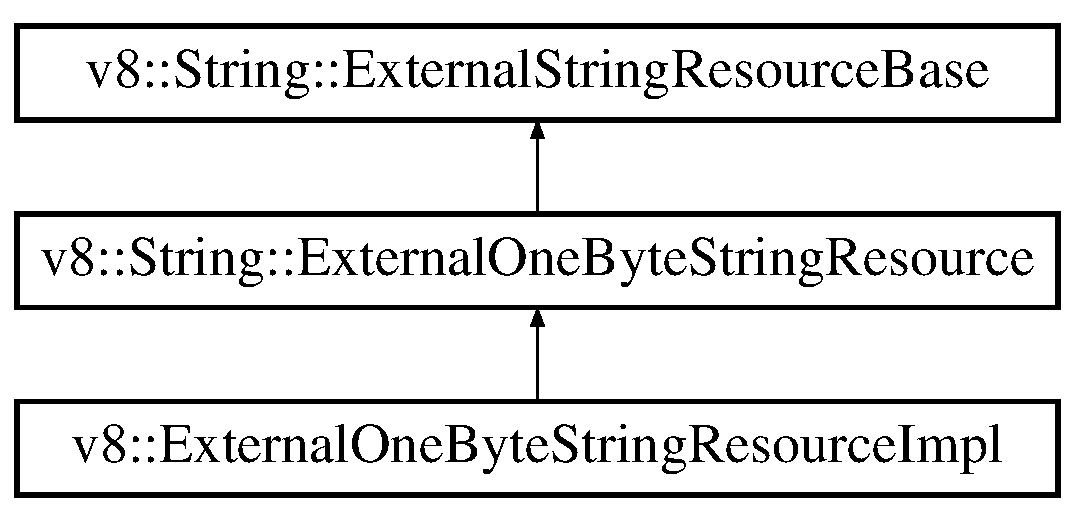
\includegraphics[height=3.000000cm]{classv8_1_1_string_1_1_external_one_byte_string_resource}
\end{center}
\end{figure}
\subsection*{Public Member Functions}
\begin{DoxyCompactItemize}
\item 
virtual \hyperlink{classv8_1_1_string_1_1_external_one_byte_string_resource_a443edbb33926b2a9480fe0caac6e95ab}{$\sim$\+External\+One\+Byte\+String\+Resource} ()
\item 
virtual const char $\ast$ \hyperlink{classv8_1_1_string_1_1_external_one_byte_string_resource_ac6183fe16dcb0d6f2906f7caf7ff1163}{data} () const  =0
\item 
virtual size\+\_\+t \hyperlink{classv8_1_1_string_1_1_external_one_byte_string_resource_aa1db65afab54efe13daf6bd39f2ad265}{length} () const  =0
\end{DoxyCompactItemize}
\subsection*{Additional Inherited Members}


\subsection{Detailed Description}
An \hyperlink{classv8_1_1_string_1_1_external_one_byte_string_resource}{External\+One\+Byte\+String\+Resource} is a wrapper around an one-\/byte string buffer that resides outside \hyperlink{classv8_1_1_v8}{V8}\textquotesingle{}s heap. Implement an \hyperlink{classv8_1_1_string_1_1_external_one_byte_string_resource}{External\+One\+Byte\+String\+Resource} to manage the life cycle of the underlying buffer. Note that the string data must be immutable and that the data must be Latin-\/1 and not U\+T\+F-\/8, which would require special treatment internally in the engine and do not allow efficient indexing. Use String\+::\+New or convert to 16 bit data for non-\/\+Latin1. 

\subsection{Constructor \& Destructor Documentation}
\index{v8\+::\+String\+::\+External\+One\+Byte\+String\+Resource@{v8\+::\+String\+::\+External\+One\+Byte\+String\+Resource}!````~External\+One\+Byte\+String\+Resource@{$\sim$\+External\+One\+Byte\+String\+Resource}}
\index{````~External\+One\+Byte\+String\+Resource@{$\sim$\+External\+One\+Byte\+String\+Resource}!v8\+::\+String\+::\+External\+One\+Byte\+String\+Resource@{v8\+::\+String\+::\+External\+One\+Byte\+String\+Resource}}
\subsubsection[{\texorpdfstring{$\sim$\+External\+One\+Byte\+String\+Resource()}{~ExternalOneByteStringResource()}}]{\setlength{\rightskip}{0pt plus 5cm}virtual v8\+::\+String\+::\+External\+One\+Byte\+String\+Resource\+::$\sim$\+External\+One\+Byte\+String\+Resource (
\begin{DoxyParamCaption}
{}
\end{DoxyParamCaption}
)\hspace{0.3cm}{\ttfamily [inline]}, {\ttfamily [virtual]}}\hypertarget{classv8_1_1_string_1_1_external_one_byte_string_resource_a443edbb33926b2a9480fe0caac6e95ab}{}\label{classv8_1_1_string_1_1_external_one_byte_string_resource_a443edbb33926b2a9480fe0caac6e95ab}
Override the destructor to manage the life cycle of the underlying buffer. 

\subsection{Member Function Documentation}
\index{v8\+::\+String\+::\+External\+One\+Byte\+String\+Resource@{v8\+::\+String\+::\+External\+One\+Byte\+String\+Resource}!data@{data}}
\index{data@{data}!v8\+::\+String\+::\+External\+One\+Byte\+String\+Resource@{v8\+::\+String\+::\+External\+One\+Byte\+String\+Resource}}
\subsubsection[{\texorpdfstring{data() const  =0}{data() const  =0}}]{\setlength{\rightskip}{0pt plus 5cm}virtual const char$\ast$ v8\+::\+String\+::\+External\+One\+Byte\+String\+Resource\+::data (
\begin{DoxyParamCaption}
{}
\end{DoxyParamCaption}
) const\hspace{0.3cm}{\ttfamily [pure virtual]}}\hypertarget{classv8_1_1_string_1_1_external_one_byte_string_resource_ac6183fe16dcb0d6f2906f7caf7ff1163}{}\label{classv8_1_1_string_1_1_external_one_byte_string_resource_ac6183fe16dcb0d6f2906f7caf7ff1163}
The string data from the underlying buffer. 

Implemented in \hyperlink{classv8_1_1_external_one_byte_string_resource_impl_a37ada5dc21ecb982c50482c90fffe529}{v8\+::\+External\+One\+Byte\+String\+Resource\+Impl}, and \hyperlink{classv8_1_1internal_1_1_natives_external_string_resource_a14cd7f1c97e77da7265ef71613b80e04}{v8\+::internal\+::\+Natives\+External\+String\+Resource}.

\index{v8\+::\+String\+::\+External\+One\+Byte\+String\+Resource@{v8\+::\+String\+::\+External\+One\+Byte\+String\+Resource}!length@{length}}
\index{length@{length}!v8\+::\+String\+::\+External\+One\+Byte\+String\+Resource@{v8\+::\+String\+::\+External\+One\+Byte\+String\+Resource}}
\subsubsection[{\texorpdfstring{length() const  =0}{length() const  =0}}]{\setlength{\rightskip}{0pt plus 5cm}virtual size\+\_\+t v8\+::\+String\+::\+External\+One\+Byte\+String\+Resource\+::length (
\begin{DoxyParamCaption}
{}
\end{DoxyParamCaption}
) const\hspace{0.3cm}{\ttfamily [pure virtual]}}\hypertarget{classv8_1_1_string_1_1_external_one_byte_string_resource_aa1db65afab54efe13daf6bd39f2ad265}{}\label{classv8_1_1_string_1_1_external_one_byte_string_resource_aa1db65afab54efe13daf6bd39f2ad265}
The number of Latin-\/1 characters in the string. 

Implemented in \hyperlink{classv8_1_1_external_one_byte_string_resource_impl_aedcf350d46f64cf1e3045658920d1dc8}{v8\+::\+External\+One\+Byte\+String\+Resource\+Impl}, and \hyperlink{classv8_1_1internal_1_1_natives_external_string_resource_adf9b2887776410671dfb32353e0d227e}{v8\+::internal\+::\+Natives\+External\+String\+Resource}.



The documentation for this class was generated from the following file\+:\begin{DoxyCompactItemize}
\item 
/\+Users/joshgav/node/v8/include/v8.\+h\end{DoxyCompactItemize}

\hypertarget{classv8_1_1_external_one_byte_string_resource_impl}{}\section{v8\+:\+:External\+One\+Byte\+String\+Resource\+Impl Class Reference}
\label{classv8_1_1_external_one_byte_string_resource_impl}\index{v8\+::\+External\+One\+Byte\+String\+Resource\+Impl@{v8\+::\+External\+One\+Byte\+String\+Resource\+Impl}}
Inheritance diagram for v8\+:\+:External\+One\+Byte\+String\+Resource\+Impl\+:\begin{figure}[H]
\begin{center}
\leavevmode
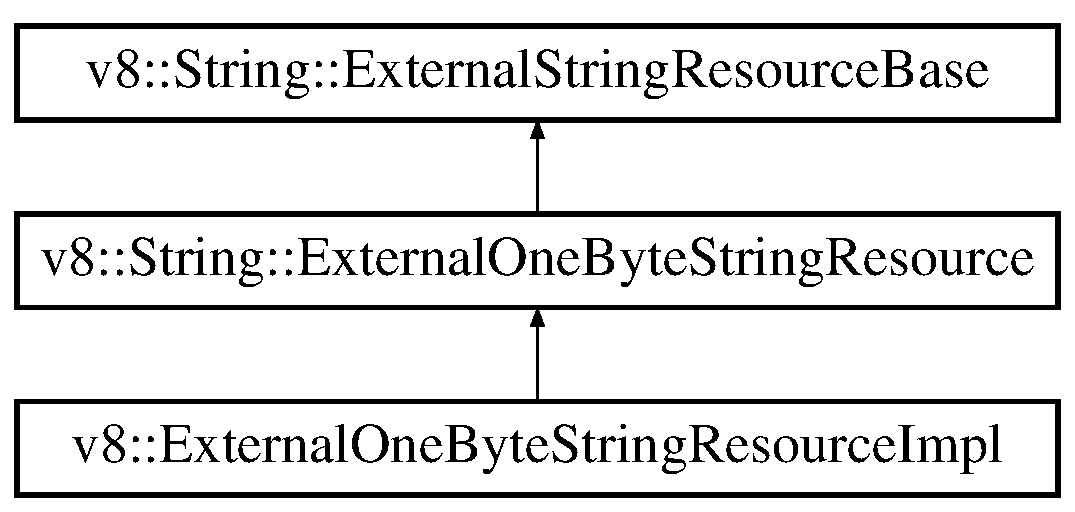
\includegraphics[height=3.000000cm]{classv8_1_1_external_one_byte_string_resource_impl}
\end{center}
\end{figure}
\subsection*{Public Member Functions}
\begin{DoxyCompactItemize}
\item 
{\bfseries External\+One\+Byte\+String\+Resource\+Impl} (const char $\ast$\hyperlink{classv8_1_1_external_one_byte_string_resource_impl_a37ada5dc21ecb982c50482c90fffe529}{data}, size\+\_\+t \hyperlink{classv8_1_1_external_one_byte_string_resource_impl_aedcf350d46f64cf1e3045658920d1dc8}{length})\hypertarget{classv8_1_1_external_one_byte_string_resource_impl_a46178fb208419f5ea99552871b3a373e}{}\label{classv8_1_1_external_one_byte_string_resource_impl_a46178fb208419f5ea99552871b3a373e}

\item 
const char $\ast$ \hyperlink{classv8_1_1_external_one_byte_string_resource_impl_a37ada5dc21ecb982c50482c90fffe529}{data} () const 
\item 
size\+\_\+t \hyperlink{classv8_1_1_external_one_byte_string_resource_impl_aedcf350d46f64cf1e3045658920d1dc8}{length} () const 
\end{DoxyCompactItemize}
\subsection*{Private Attributes}
\begin{DoxyCompactItemize}
\item 
const char $\ast$ {\bfseries data\+\_\+}\hypertarget{classv8_1_1_external_one_byte_string_resource_impl_a1ffd1e433e1d12bec9211bfa1804c01b}{}\label{classv8_1_1_external_one_byte_string_resource_impl_a1ffd1e433e1d12bec9211bfa1804c01b}

\item 
size\+\_\+t {\bfseries length\+\_\+}\hypertarget{classv8_1_1_external_one_byte_string_resource_impl_a915f91ba58fef447920672ad6d11711f}{}\label{classv8_1_1_external_one_byte_string_resource_impl_a915f91ba58fef447920672ad6d11711f}

\end{DoxyCompactItemize}
\subsection*{Additional Inherited Members}


\subsection{Member Function Documentation}
\index{v8\+::\+External\+One\+Byte\+String\+Resource\+Impl@{v8\+::\+External\+One\+Byte\+String\+Resource\+Impl}!data@{data}}
\index{data@{data}!v8\+::\+External\+One\+Byte\+String\+Resource\+Impl@{v8\+::\+External\+One\+Byte\+String\+Resource\+Impl}}
\subsubsection[{\texorpdfstring{data() const }{data() const }}]{\setlength{\rightskip}{0pt plus 5cm}const char$\ast$ v8\+::\+External\+One\+Byte\+String\+Resource\+Impl\+::data (
\begin{DoxyParamCaption}
{}
\end{DoxyParamCaption}
) const\hspace{0.3cm}{\ttfamily [inline]}, {\ttfamily [virtual]}}\hypertarget{classv8_1_1_external_one_byte_string_resource_impl_a37ada5dc21ecb982c50482c90fffe529}{}\label{classv8_1_1_external_one_byte_string_resource_impl_a37ada5dc21ecb982c50482c90fffe529}
The string data from the underlying buffer. 

Implements \hyperlink{classv8_1_1_string_1_1_external_one_byte_string_resource_ac6183fe16dcb0d6f2906f7caf7ff1163}{v8\+::\+String\+::\+External\+One\+Byte\+String\+Resource}.

\index{v8\+::\+External\+One\+Byte\+String\+Resource\+Impl@{v8\+::\+External\+One\+Byte\+String\+Resource\+Impl}!length@{length}}
\index{length@{length}!v8\+::\+External\+One\+Byte\+String\+Resource\+Impl@{v8\+::\+External\+One\+Byte\+String\+Resource\+Impl}}
\subsubsection[{\texorpdfstring{length() const }{length() const }}]{\setlength{\rightskip}{0pt plus 5cm}size\+\_\+t v8\+::\+External\+One\+Byte\+String\+Resource\+Impl\+::length (
\begin{DoxyParamCaption}
{}
\end{DoxyParamCaption}
) const\hspace{0.3cm}{\ttfamily [inline]}, {\ttfamily [virtual]}}\hypertarget{classv8_1_1_external_one_byte_string_resource_impl_aedcf350d46f64cf1e3045658920d1dc8}{}\label{classv8_1_1_external_one_byte_string_resource_impl_aedcf350d46f64cf1e3045658920d1dc8}
The number of Latin-\/1 characters in the string. 

Implements \hyperlink{classv8_1_1_string_1_1_external_one_byte_string_resource_aa1db65afab54efe13daf6bd39f2ad265}{v8\+::\+String\+::\+External\+One\+Byte\+String\+Resource}.



The documentation for this class was generated from the following file\+:\begin{DoxyCompactItemize}
\item 
/\+Users/joshgav/node/v8/include/v8.\+h\end{DoxyCompactItemize}

\hypertarget{classv8_1_1_external_resource_visitor}{}\section{v8\+:\+:External\+Resource\+Visitor Class Reference}
\label{classv8_1_1_external_resource_visitor}\index{v8\+::\+External\+Resource\+Visitor@{v8\+::\+External\+Resource\+Visitor}}


{\ttfamily \#include $<$v8.\+h$>$}

\subsection*{Public Member Functions}
\begin{DoxyCompactItemize}
\item 
virtual void {\bfseries Visit\+External\+String} (\hyperlink{classv8_1_1_local}{Local}$<$ \hyperlink{classv8_1_1_string}{String} $>$ string)\hypertarget{classv8_1_1_external_resource_visitor_ad611b1b6a06753f8eaf6936f793441bd}{}\label{classv8_1_1_external_resource_visitor_ad611b1b6a06753f8eaf6936f793441bd}

\end{DoxyCompactItemize}


\subsection{Detailed Description}
Interface for iterating through all external resources in the heap. 

The documentation for this class was generated from the following file\+:\begin{DoxyCompactItemize}
\item 
/\+Users/joshgav/node/v8/include/v8.\+h\end{DoxyCompactItemize}

\hypertarget{classv8_1_1_script_compiler_1_1_external_source_stream}{}\section{v8\+:\+:Script\+Compiler\+:\+:External\+Source\+Stream Class Reference}
\label{classv8_1_1_script_compiler_1_1_external_source_stream}\index{v8\+::\+Script\+Compiler\+::\+External\+Source\+Stream@{v8\+::\+Script\+Compiler\+::\+External\+Source\+Stream}}


{\ttfamily \#include $<$v8.\+h$>$}

\subsection*{Public Member Functions}
\begin{DoxyCompactItemize}
\item 
virtual size\+\_\+t \hyperlink{classv8_1_1_script_compiler_1_1_external_source_stream_ac3a0221b5725f0b612a6342d8e83d899}{Get\+More\+Data} (const uint8\+\_\+t $\ast$$\ast$src)=0
\item 
virtual bool \hyperlink{classv8_1_1_script_compiler_1_1_external_source_stream_a0012cebde92a3a61ec033e3abc2dd2ee}{Set\+Bookmark} ()
\item 
virtual void \hyperlink{classv8_1_1_script_compiler_1_1_external_source_stream_af950fd00676e6bdb8642791f651b161a}{Reset\+To\+Bookmark} ()
\end{DoxyCompactItemize}


\subsection{Detailed Description}
For streaming incomplete script data to \hyperlink{classv8_1_1_v8}{V8}. The embedder should implement a subclass of this class. 

\subsection{Member Function Documentation}
\index{v8\+::\+Script\+Compiler\+::\+External\+Source\+Stream@{v8\+::\+Script\+Compiler\+::\+External\+Source\+Stream}!Get\+More\+Data@{Get\+More\+Data}}
\index{Get\+More\+Data@{Get\+More\+Data}!v8\+::\+Script\+Compiler\+::\+External\+Source\+Stream@{v8\+::\+Script\+Compiler\+::\+External\+Source\+Stream}}
\subsubsection[{\texorpdfstring{Get\+More\+Data(const uint8\+\_\+t $\ast$$\ast$src)=0}{GetMoreData(const uint8_t **src)=0}}]{\setlength{\rightskip}{0pt plus 5cm}virtual size\+\_\+t v8\+::\+Script\+Compiler\+::\+External\+Source\+Stream\+::\+Get\+More\+Data (
\begin{DoxyParamCaption}
\item[{const uint8\+\_\+t $\ast$$\ast$}]{src}
\end{DoxyParamCaption}
)\hspace{0.3cm}{\ttfamily [pure virtual]}}\hypertarget{classv8_1_1_script_compiler_1_1_external_source_stream_ac3a0221b5725f0b612a6342d8e83d899}{}\label{classv8_1_1_script_compiler_1_1_external_source_stream_ac3a0221b5725f0b612a6342d8e83d899}
\hyperlink{classv8_1_1_v8}{V8} calls this to request the next chunk of data from the embedder. This function will be called on a background thread, so it\textquotesingle{}s OK to block and wait for the data, if the embedder doesn\textquotesingle{}t have data yet. Returns the length of the data returned. When the data ends, Get\+More\+Data should return 0. Caller takes ownership of the data.

When streaming U\+T\+F-\/8 data, \hyperlink{classv8_1_1_v8}{V8} handles multi-\/byte characters split between two data chunks, but doesn\textquotesingle{}t handle multi-\/byte characters split between more than two data chunks. The embedder can avoid this problem by always returning at least 2 bytes of data.

If the embedder wants to cancel the streaming, they should make the next Get\+More\+Data call return 0. \hyperlink{classv8_1_1_v8}{V8} will interpret it as end of data (and most probably, parsing will fail). The streaming task will return as soon as \hyperlink{classv8_1_1_v8}{V8} has parsed the data it received so far. \index{v8\+::\+Script\+Compiler\+::\+External\+Source\+Stream@{v8\+::\+Script\+Compiler\+::\+External\+Source\+Stream}!Reset\+To\+Bookmark@{Reset\+To\+Bookmark}}
\index{Reset\+To\+Bookmark@{Reset\+To\+Bookmark}!v8\+::\+Script\+Compiler\+::\+External\+Source\+Stream@{v8\+::\+Script\+Compiler\+::\+External\+Source\+Stream}}
\subsubsection[{\texorpdfstring{Reset\+To\+Bookmark()}{ResetToBookmark()}}]{\setlength{\rightskip}{0pt plus 5cm}void v8\+::\+Script\+Compiler\+::\+External\+Source\+Stream\+::\+Reset\+To\+Bookmark (
\begin{DoxyParamCaption}
{}
\end{DoxyParamCaption}
)\hspace{0.3cm}{\ttfamily [virtual]}}\hypertarget{classv8_1_1_script_compiler_1_1_external_source_stream_af950fd00676e6bdb8642791f651b161a}{}\label{classv8_1_1_script_compiler_1_1_external_source_stream_af950fd00676e6bdb8642791f651b161a}
\hyperlink{classv8_1_1_v8}{V8} calls this to return to a previously set bookmark. \index{v8\+::\+Script\+Compiler\+::\+External\+Source\+Stream@{v8\+::\+Script\+Compiler\+::\+External\+Source\+Stream}!Set\+Bookmark@{Set\+Bookmark}}
\index{Set\+Bookmark@{Set\+Bookmark}!v8\+::\+Script\+Compiler\+::\+External\+Source\+Stream@{v8\+::\+Script\+Compiler\+::\+External\+Source\+Stream}}
\subsubsection[{\texorpdfstring{Set\+Bookmark()}{SetBookmark()}}]{\setlength{\rightskip}{0pt plus 5cm}bool v8\+::\+Script\+Compiler\+::\+External\+Source\+Stream\+::\+Set\+Bookmark (
\begin{DoxyParamCaption}
{}
\end{DoxyParamCaption}
)\hspace{0.3cm}{\ttfamily [virtual]}}\hypertarget{classv8_1_1_script_compiler_1_1_external_source_stream_a0012cebde92a3a61ec033e3abc2dd2ee}{}\label{classv8_1_1_script_compiler_1_1_external_source_stream_a0012cebde92a3a61ec033e3abc2dd2ee}
\hyperlink{classv8_1_1_v8}{V8} calls this method to set a \textquotesingle{}bookmark\textquotesingle{} at the current position in the source stream, for the purpose of (maybe) later calling Reset\+To\+Bookmark. If Reset\+To\+Bookmark is called later, then subsequent calls to Get\+More\+Data should return the same data as they did when Set\+Bookmark was called earlier.

The embedder may return \textquotesingle{}false\textquotesingle{} to indicate it cannot provide this functionality. 

The documentation for this class was generated from the following files\+:\begin{DoxyCompactItemize}
\item 
/\+Users/joshgav/node/v8/include/v8.\+h\item 
/\+Users/joshgav/node/v8/src/api.\+cc\end{DoxyCompactItemize}

\hypertarget{classv8_1_1_string_1_1_external_string_resource}{}\section{v8\+:\+:String\+:\+:External\+String\+Resource Class Reference}
\label{classv8_1_1_string_1_1_external_string_resource}\index{v8\+::\+String\+::\+External\+String\+Resource@{v8\+::\+String\+::\+External\+String\+Resource}}


{\ttfamily \#include $<$v8.\+h$>$}

Inheritance diagram for v8\+:\+:String\+:\+:External\+String\+Resource\+:\begin{figure}[H]
\begin{center}
\leavevmode
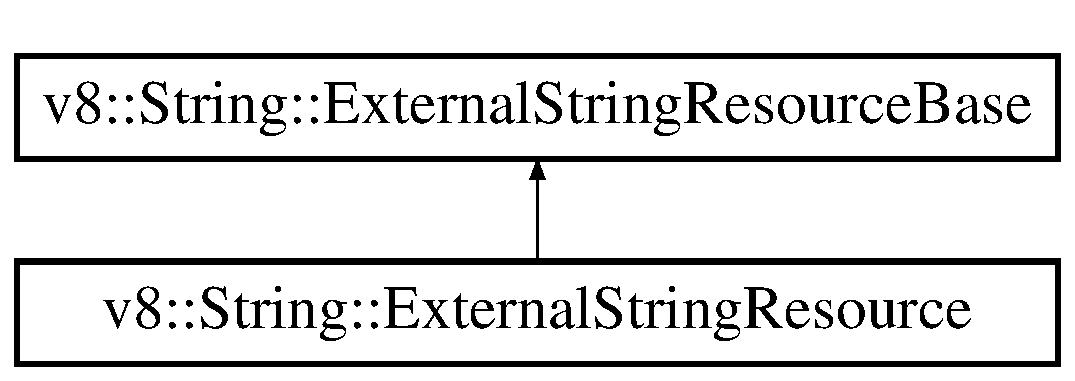
\includegraphics[height=2.000000cm]{classv8_1_1_string_1_1_external_string_resource}
\end{center}
\end{figure}
\subsection*{Public Member Functions}
\begin{DoxyCompactItemize}
\item 
virtual \hyperlink{classv8_1_1_string_1_1_external_string_resource_a6b7ef9e33a47059092e1447b10c35416}{$\sim$\+External\+String\+Resource} ()
\item 
virtual const uint16\+\_\+t $\ast$ \hyperlink{classv8_1_1_string_1_1_external_string_resource_a53ca87d049fc8bfea5944adde4e7b159}{data} () const  =0
\item 
virtual size\+\_\+t \hyperlink{classv8_1_1_string_1_1_external_string_resource_af6c1b3f63e2e3112da788928aac96fab}{length} () const  =0
\end{DoxyCompactItemize}
\subsection*{Additional Inherited Members}


\subsection{Detailed Description}
An \hyperlink{classv8_1_1_string_1_1_external_string_resource}{External\+String\+Resource} is a wrapper around a two-\/byte string buffer that resides outside \hyperlink{classv8_1_1_v8}{V8}\textquotesingle{}s heap. Implement an \hyperlink{classv8_1_1_string_1_1_external_string_resource}{External\+String\+Resource} to manage the life cycle of the underlying buffer. Note that the string data must be immutable. 

\subsection{Constructor \& Destructor Documentation}
\index{v8\+::\+String\+::\+External\+String\+Resource@{v8\+::\+String\+::\+External\+String\+Resource}!````~External\+String\+Resource@{$\sim$\+External\+String\+Resource}}
\index{````~External\+String\+Resource@{$\sim$\+External\+String\+Resource}!v8\+::\+String\+::\+External\+String\+Resource@{v8\+::\+String\+::\+External\+String\+Resource}}
\subsubsection[{\texorpdfstring{$\sim$\+External\+String\+Resource()}{~ExternalStringResource()}}]{\setlength{\rightskip}{0pt plus 5cm}virtual v8\+::\+String\+::\+External\+String\+Resource\+::$\sim$\+External\+String\+Resource (
\begin{DoxyParamCaption}
{}
\end{DoxyParamCaption}
)\hspace{0.3cm}{\ttfamily [inline]}, {\ttfamily [virtual]}}\hypertarget{classv8_1_1_string_1_1_external_string_resource_a6b7ef9e33a47059092e1447b10c35416}{}\label{classv8_1_1_string_1_1_external_string_resource_a6b7ef9e33a47059092e1447b10c35416}
Override the destructor to manage the life cycle of the underlying buffer. 

\subsection{Member Function Documentation}
\index{v8\+::\+String\+::\+External\+String\+Resource@{v8\+::\+String\+::\+External\+String\+Resource}!data@{data}}
\index{data@{data}!v8\+::\+String\+::\+External\+String\+Resource@{v8\+::\+String\+::\+External\+String\+Resource}}
\subsubsection[{\texorpdfstring{data() const  =0}{data() const  =0}}]{\setlength{\rightskip}{0pt plus 5cm}virtual const uint16\+\_\+t$\ast$ v8\+::\+String\+::\+External\+String\+Resource\+::data (
\begin{DoxyParamCaption}
{}
\end{DoxyParamCaption}
) const\hspace{0.3cm}{\ttfamily [pure virtual]}}\hypertarget{classv8_1_1_string_1_1_external_string_resource_a53ca87d049fc8bfea5944adde4e7b159}{}\label{classv8_1_1_string_1_1_external_string_resource_a53ca87d049fc8bfea5944adde4e7b159}
The string data from the underlying buffer. \index{v8\+::\+String\+::\+External\+String\+Resource@{v8\+::\+String\+::\+External\+String\+Resource}!length@{length}}
\index{length@{length}!v8\+::\+String\+::\+External\+String\+Resource@{v8\+::\+String\+::\+External\+String\+Resource}}
\subsubsection[{\texorpdfstring{length() const  =0}{length() const  =0}}]{\setlength{\rightskip}{0pt plus 5cm}virtual size\+\_\+t v8\+::\+String\+::\+External\+String\+Resource\+::length (
\begin{DoxyParamCaption}
{}
\end{DoxyParamCaption}
) const\hspace{0.3cm}{\ttfamily [pure virtual]}}\hypertarget{classv8_1_1_string_1_1_external_string_resource_af6c1b3f63e2e3112da788928aac96fab}{}\label{classv8_1_1_string_1_1_external_string_resource_af6c1b3f63e2e3112da788928aac96fab}
The length of the string. That is, the number of two-\/byte characters. 

The documentation for this class was generated from the following file\+:\begin{DoxyCompactItemize}
\item 
include/v8.\+h\end{DoxyCompactItemize}

\hypertarget{classv8_1_1_string_1_1_external_string_resource_base}{}\section{v8\+:\+:String\+:\+:External\+String\+Resource\+Base Class Reference}
\label{classv8_1_1_string_1_1_external_string_resource_base}\index{v8\+::\+String\+::\+External\+String\+Resource\+Base@{v8\+::\+String\+::\+External\+String\+Resource\+Base}}
Inheritance diagram for v8\+:\+:String\+:\+:External\+String\+Resource\+Base\+:\begin{figure}[H]
\begin{center}
\leavevmode
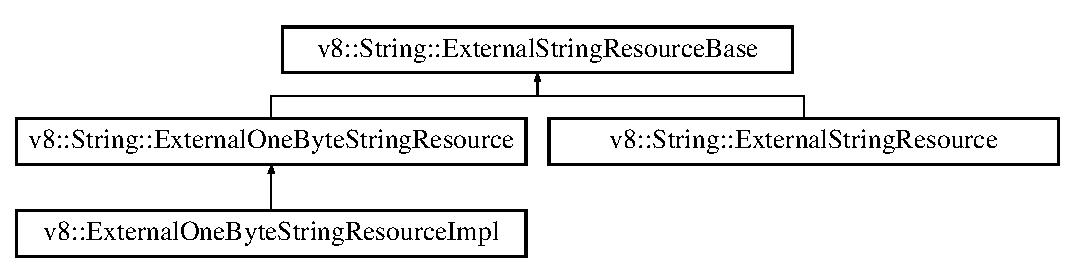
\includegraphics[height=3.000000cm]{classv8_1_1_string_1_1_external_string_resource_base}
\end{center}
\end{figure}
\subsection*{Public Member Functions}
\begin{DoxyCompactItemize}
\item 
virtual bool {\bfseries Is\+Compressible} () const \hypertarget{classv8_1_1_string_1_1_external_string_resource_base_ace144d07dbe4e91665ee3ee22635e365}{}\label{classv8_1_1_string_1_1_external_string_resource_base_ace144d07dbe4e91665ee3ee22635e365}

\end{DoxyCompactItemize}
\subsection*{Protected Member Functions}
\begin{DoxyCompactItemize}
\item 
virtual void \hyperlink{classv8_1_1_string_1_1_external_string_resource_base_af4720342ae31e1ab4656df3f15d069c0}{Dispose} ()
\end{DoxyCompactItemize}
\subsection*{Private Member Functions}
\begin{DoxyCompactItemize}
\item 
{\bfseries External\+String\+Resource\+Base} (const \hyperlink{classv8_1_1_string_1_1_external_string_resource_base}{External\+String\+Resource\+Base} \&)\hypertarget{classv8_1_1_string_1_1_external_string_resource_base_a04c9e0ef835b5a27f4a6e97387cb5f1b}{}\label{classv8_1_1_string_1_1_external_string_resource_base_a04c9e0ef835b5a27f4a6e97387cb5f1b}

\item 
void {\bfseries operator=} (const \hyperlink{classv8_1_1_string_1_1_external_string_resource_base}{External\+String\+Resource\+Base} \&)\hypertarget{classv8_1_1_string_1_1_external_string_resource_base_a8bee080ff920e233dd72cf336081b4d2}{}\label{classv8_1_1_string_1_1_external_string_resource_base_a8bee080ff920e233dd72cf336081b4d2}

\end{DoxyCompactItemize}
\subsection*{Friends}
\begin{DoxyCompactItemize}
\item 
class {\bfseries v8\+::internal\+::\+Heap}\hypertarget{classv8_1_1_string_1_1_external_string_resource_base_a2d52f783e6ad51ce2c8f89eb1ebc7599}{}\label{classv8_1_1_string_1_1_external_string_resource_base_a2d52f783e6ad51ce2c8f89eb1ebc7599}

\end{DoxyCompactItemize}


\subsection{Member Function Documentation}
\index{v8\+::\+String\+::\+External\+String\+Resource\+Base@{v8\+::\+String\+::\+External\+String\+Resource\+Base}!Dispose@{Dispose}}
\index{Dispose@{Dispose}!v8\+::\+String\+::\+External\+String\+Resource\+Base@{v8\+::\+String\+::\+External\+String\+Resource\+Base}}
\subsubsection[{\texorpdfstring{Dispose()}{Dispose()}}]{\setlength{\rightskip}{0pt plus 5cm}virtual void v8\+::\+String\+::\+External\+String\+Resource\+Base\+::\+Dispose (
\begin{DoxyParamCaption}
{}
\end{DoxyParamCaption}
)\hspace{0.3cm}{\ttfamily [inline]}, {\ttfamily [protected]}, {\ttfamily [virtual]}}\hypertarget{classv8_1_1_string_1_1_external_string_resource_base_af4720342ae31e1ab4656df3f15d069c0}{}\label{classv8_1_1_string_1_1_external_string_resource_base_af4720342ae31e1ab4656df3f15d069c0}
Internally \hyperlink{classv8_1_1_v8}{V8} will call this Dispose method when the external string resource is no longer needed. The default implementation will use the delete operator. This method can be overridden in subclasses to control how allocated external string resources are disposed. 

The documentation for this class was generated from the following file\+:\begin{DoxyCompactItemize}
\item 
/\+Users/joshgav/node/v8/include/v8.\+h\end{DoxyCompactItemize}

\hypertarget{classv8_1_1experimental_1_1_fast_accessor_builder}{}\section{v8\+:\+:experimental\+:\+:Fast\+Accessor\+Builder Class Reference}
\label{classv8_1_1experimental_1_1_fast_accessor_builder}\index{v8\+::experimental\+::\+Fast\+Accessor\+Builder@{v8\+::experimental\+::\+Fast\+Accessor\+Builder}}
\subsection*{Classes}
\begin{DoxyCompactItemize}
\item 
struct \hyperlink{structv8_1_1experimental_1_1_fast_accessor_builder_1_1_label_id}{Label\+Id}
\item 
struct \hyperlink{structv8_1_1experimental_1_1_fast_accessor_builder_1_1_value_id}{Value\+Id}
\end{DoxyCompactItemize}
\subsection*{Public Member Functions}
\begin{DoxyCompactItemize}
\item 
\hyperlink{structv8_1_1experimental_1_1_fast_accessor_builder_1_1_value_id}{Value\+Id} {\bfseries Integer\+Constant} (int int\+\_\+constant)\hypertarget{classv8_1_1experimental_1_1_fast_accessor_builder_a65c37490d0d4c8db62a520f22fa6d74f}{}\label{classv8_1_1experimental_1_1_fast_accessor_builder_a65c37490d0d4c8db62a520f22fa6d74f}

\item 
\hyperlink{structv8_1_1experimental_1_1_fast_accessor_builder_1_1_value_id}{Value\+Id} {\bfseries Get\+Receiver} ()\hypertarget{classv8_1_1experimental_1_1_fast_accessor_builder_a5c3e8027771b0ddede084ae74f8e3cd9}{}\label{classv8_1_1experimental_1_1_fast_accessor_builder_a5c3e8027771b0ddede084ae74f8e3cd9}

\item 
\hyperlink{structv8_1_1experimental_1_1_fast_accessor_builder_1_1_value_id}{Value\+Id} {\bfseries Load\+Internal\+Field} (\hyperlink{structv8_1_1experimental_1_1_fast_accessor_builder_1_1_value_id}{Value\+Id} value\+\_\+id, int field\+\_\+no)\hypertarget{classv8_1_1experimental_1_1_fast_accessor_builder_a09851bca6e5d405137c3aed9e01ad2ba}{}\label{classv8_1_1experimental_1_1_fast_accessor_builder_a09851bca6e5d405137c3aed9e01ad2ba}

\item 
\hyperlink{structv8_1_1experimental_1_1_fast_accessor_builder_1_1_value_id}{Value\+Id} {\bfseries Load\+Value} (\hyperlink{structv8_1_1experimental_1_1_fast_accessor_builder_1_1_value_id}{Value\+Id} value\+\_\+id, int offset)\hypertarget{classv8_1_1experimental_1_1_fast_accessor_builder_a5056ac24836a402b51c2fde9e8fb1795}{}\label{classv8_1_1experimental_1_1_fast_accessor_builder_a5056ac24836a402b51c2fde9e8fb1795}

\item 
\hyperlink{structv8_1_1experimental_1_1_fast_accessor_builder_1_1_value_id}{Value\+Id} {\bfseries Load\+Object} (\hyperlink{structv8_1_1experimental_1_1_fast_accessor_builder_1_1_value_id}{Value\+Id} value\+\_\+id, int offset)\hypertarget{classv8_1_1experimental_1_1_fast_accessor_builder_a55fc64e70449b825f2b79a9f46d217b3}{}\label{classv8_1_1experimental_1_1_fast_accessor_builder_a55fc64e70449b825f2b79a9f46d217b3}

\item 
void {\bfseries Return\+Value} (\hyperlink{structv8_1_1experimental_1_1_fast_accessor_builder_1_1_value_id}{Value\+Id} value\+\_\+id)\hypertarget{classv8_1_1experimental_1_1_fast_accessor_builder_a1d4e664176fe26c36e23927dd26f9fbf}{}\label{classv8_1_1experimental_1_1_fast_accessor_builder_a1d4e664176fe26c36e23927dd26f9fbf}

\item 
void {\bfseries Check\+Flag\+Set\+Or\+Return\+Null} (\hyperlink{structv8_1_1experimental_1_1_fast_accessor_builder_1_1_value_id}{Value\+Id} value\+\_\+id, int mask)\hypertarget{classv8_1_1experimental_1_1_fast_accessor_builder_a9d8b37bf2973753f66bbbd8d1760342f}{}\label{classv8_1_1experimental_1_1_fast_accessor_builder_a9d8b37bf2973753f66bbbd8d1760342f}

\item 
void {\bfseries Check\+Not\+Zero\+Or\+Return\+Null} (\hyperlink{structv8_1_1experimental_1_1_fast_accessor_builder_1_1_value_id}{Value\+Id} value\+\_\+id)\hypertarget{classv8_1_1experimental_1_1_fast_accessor_builder_a9ee8c424d01ebdaebbaade38052733ec}{}\label{classv8_1_1experimental_1_1_fast_accessor_builder_a9ee8c424d01ebdaebbaade38052733ec}

\item 
\hyperlink{structv8_1_1experimental_1_1_fast_accessor_builder_1_1_label_id}{Label\+Id} {\bfseries Make\+Label} ()\hypertarget{classv8_1_1experimental_1_1_fast_accessor_builder_aa18b503a8eaaf4e51d528ec37d352271}{}\label{classv8_1_1experimental_1_1_fast_accessor_builder_aa18b503a8eaaf4e51d528ec37d352271}

\item 
void {\bfseries Set\+Label} (\hyperlink{structv8_1_1experimental_1_1_fast_accessor_builder_1_1_label_id}{Label\+Id} label\+\_\+id)\hypertarget{classv8_1_1experimental_1_1_fast_accessor_builder_add8b517b37d62c624930f2afbe20995f}{}\label{classv8_1_1experimental_1_1_fast_accessor_builder_add8b517b37d62c624930f2afbe20995f}

\item 
void {\bfseries Check\+Not\+Zero\+Or\+Jump} (\hyperlink{structv8_1_1experimental_1_1_fast_accessor_builder_1_1_value_id}{Value\+Id} value\+\_\+id, \hyperlink{structv8_1_1experimental_1_1_fast_accessor_builder_1_1_label_id}{Label\+Id} label\+\_\+id)\hypertarget{classv8_1_1experimental_1_1_fast_accessor_builder_adb6c283fcf60c19d523914cb12d092f0}{}\label{classv8_1_1experimental_1_1_fast_accessor_builder_adb6c283fcf60c19d523914cb12d092f0}

\item 
\hyperlink{structv8_1_1experimental_1_1_fast_accessor_builder_1_1_value_id}{Value\+Id} {\bfseries Call} (v8\+::\+Function\+Callback callback, \hyperlink{structv8_1_1experimental_1_1_fast_accessor_builder_1_1_value_id}{Value\+Id} value\+\_\+id)\hypertarget{classv8_1_1experimental_1_1_fast_accessor_builder_a90fbd0d3836e8ae836e1097166862d80}{}\label{classv8_1_1experimental_1_1_fast_accessor_builder_a90fbd0d3836e8ae836e1097166862d80}

\end{DoxyCompactItemize}
\subsection*{Static Public Member Functions}
\begin{DoxyCompactItemize}
\item 
static \hyperlink{classv8_1_1experimental_1_1_fast_accessor_builder}{Fast\+Accessor\+Builder} $\ast$ {\bfseries New} (\hyperlink{classv8_1_1_isolate}{Isolate} $\ast$isolate)\hypertarget{classv8_1_1experimental_1_1_fast_accessor_builder_a08c581575cd9eda62d48c79c05900909}{}\label{classv8_1_1experimental_1_1_fast_accessor_builder_a08c581575cd9eda62d48c79c05900909}

\end{DoxyCompactItemize}
\subsection*{Private Member Functions}
\begin{DoxyCompactItemize}
\item 
{\bfseries Fast\+Accessor\+Builder} (const \hyperlink{classv8_1_1experimental_1_1_fast_accessor_builder}{Fast\+Accessor\+Builder} \&)=delete\hypertarget{classv8_1_1experimental_1_1_fast_accessor_builder_aad57de2056ac00fc77a8b9c5d9ff9951}{}\label{classv8_1_1experimental_1_1_fast_accessor_builder_aad57de2056ac00fc77a8b9c5d9ff9951}

\item 
void {\bfseries operator=} (const \hyperlink{classv8_1_1experimental_1_1_fast_accessor_builder}{Fast\+Accessor\+Builder} \&)=delete\hypertarget{classv8_1_1experimental_1_1_fast_accessor_builder_a9293ec9344bae9e233b9155651458f8c}{}\label{classv8_1_1experimental_1_1_fast_accessor_builder_a9293ec9344bae9e233b9155651458f8c}

\end{DoxyCompactItemize}


The documentation for this class was generated from the following files\+:\begin{DoxyCompactItemize}
\item 
/\+Users/joshgav/node/v8/include/v8-\/experimental.\+h\item 
/\+Users/joshgav/node/v8/src/api-\/experimental.\+cc\end{DoxyCompactItemize}

\hypertarget{classv8_1_1_float32_array}{}\section{v8\+:\+:Float32\+Array Class Reference}
\label{classv8_1_1_float32_array}\index{v8\+::\+Float32\+Array@{v8\+::\+Float32\+Array}}


{\ttfamily \#include $<$v8.\+h$>$}

Inheritance diagram for v8\+:\+:Float32\+Array\+:\begin{figure}[H]
\begin{center}
\leavevmode
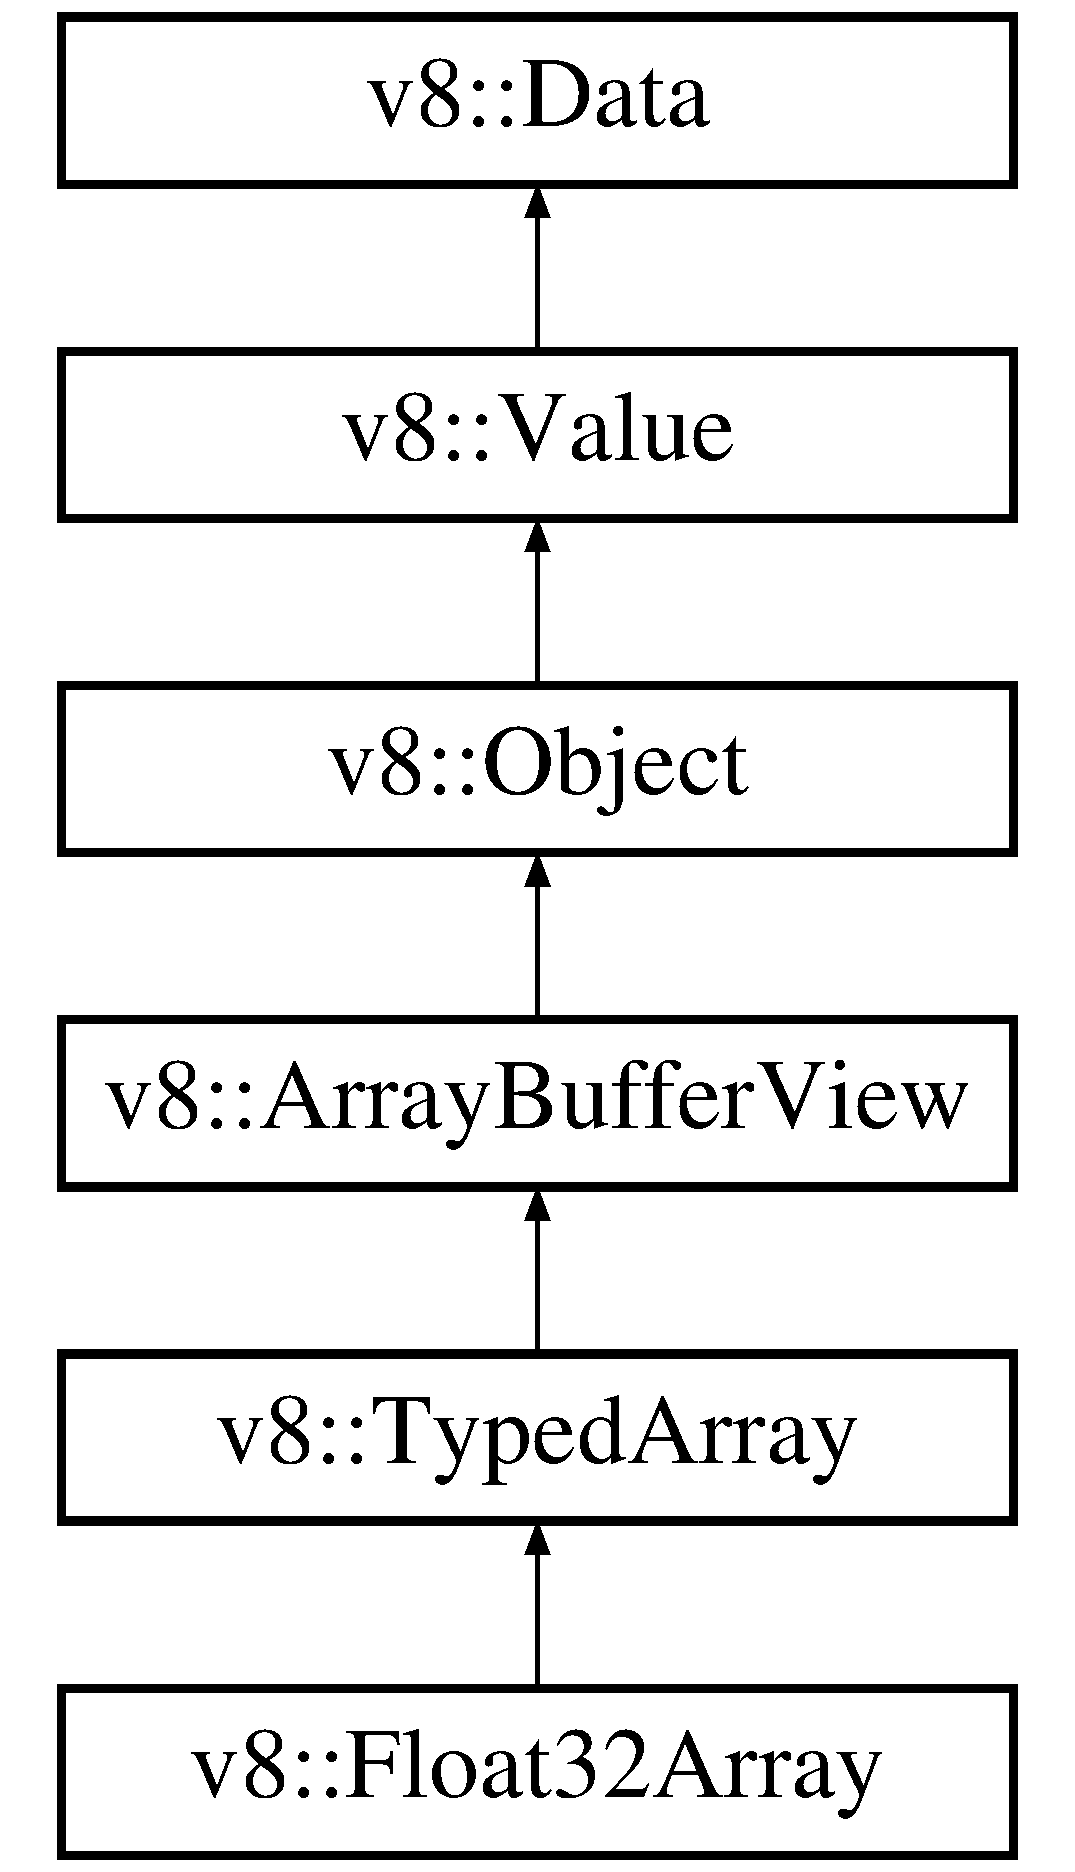
\includegraphics[height=6.000000cm]{classv8_1_1_float32_array}
\end{center}
\end{figure}
\subsection*{Static Public Member Functions}
\begin{DoxyCompactItemize}
\item 
static \hyperlink{classv8_1_1_local}{Local}$<$ \hyperlink{classv8_1_1_float32_array}{Float32\+Array} $>$ {\bfseries New} (\hyperlink{classv8_1_1_local}{Local}$<$ \hyperlink{classv8_1_1_array_buffer}{Array\+Buffer} $>$ array\+\_\+buffer, size\+\_\+t byte\+\_\+offset, size\+\_\+t length)\hypertarget{classv8_1_1_float32_array_af7e2ce97268849289d8ab38fd07fbf62}{}\label{classv8_1_1_float32_array_af7e2ce97268849289d8ab38fd07fbf62}

\item 
static \hyperlink{classv8_1_1_local}{Local}$<$ \hyperlink{classv8_1_1_float32_array}{Float32\+Array} $>$ {\bfseries New} (\hyperlink{classv8_1_1_local}{Local}$<$ \hyperlink{classv8_1_1_shared_array_buffer}{Shared\+Array\+Buffer} $>$ shared\+\_\+array\+\_\+buffer, size\+\_\+t byte\+\_\+offset, size\+\_\+t length)\hypertarget{classv8_1_1_float32_array_af3140edf1f13845670f4e4ddd41200c3}{}\label{classv8_1_1_float32_array_af3140edf1f13845670f4e4ddd41200c3}

\item 
static V8\+\_\+\+I\+N\+L\+I\+NE \hyperlink{classv8_1_1_float32_array}{Float32\+Array} $\ast$ {\bfseries Cast} (\hyperlink{classv8_1_1_value}{Value} $\ast$obj)\hypertarget{classv8_1_1_float32_array_adf926d03cacd4b3901d7f9750671a350}{}\label{classv8_1_1_float32_array_adf926d03cacd4b3901d7f9750671a350}

\end{DoxyCompactItemize}
\subsection*{Static Private Member Functions}
\begin{DoxyCompactItemize}
\item 
static void {\bfseries Check\+Cast} (\hyperlink{classv8_1_1_value}{Value} $\ast$obj)\hypertarget{classv8_1_1_float32_array_a5b68fdb621cc7e0483b652c8d49133b2}{}\label{classv8_1_1_float32_array_a5b68fdb621cc7e0483b652c8d49133b2}

\end{DoxyCompactItemize}
\subsection*{Additional Inherited Members}


\subsection{Detailed Description}
An instance of \hyperlink{classv8_1_1_float32_array}{Float32\+Array} constructor (E\+S6 draft 15.\+13.\+6). This A\+PI is experimental and may change significantly. 

The documentation for this class was generated from the following file\+:\begin{DoxyCompactItemize}
\item 
include/v8.\+h\end{DoxyCompactItemize}

\hypertarget{classv8_1_1_float64_array}{}\section{v8\+:\+:Float64\+Array Class Reference}
\label{classv8_1_1_float64_array}\index{v8\+::\+Float64\+Array@{v8\+::\+Float64\+Array}}


{\ttfamily \#include $<$v8.\+h$>$}

Inheritance diagram for v8\+:\+:Float64\+Array\+:\begin{figure}[H]
\begin{center}
\leavevmode
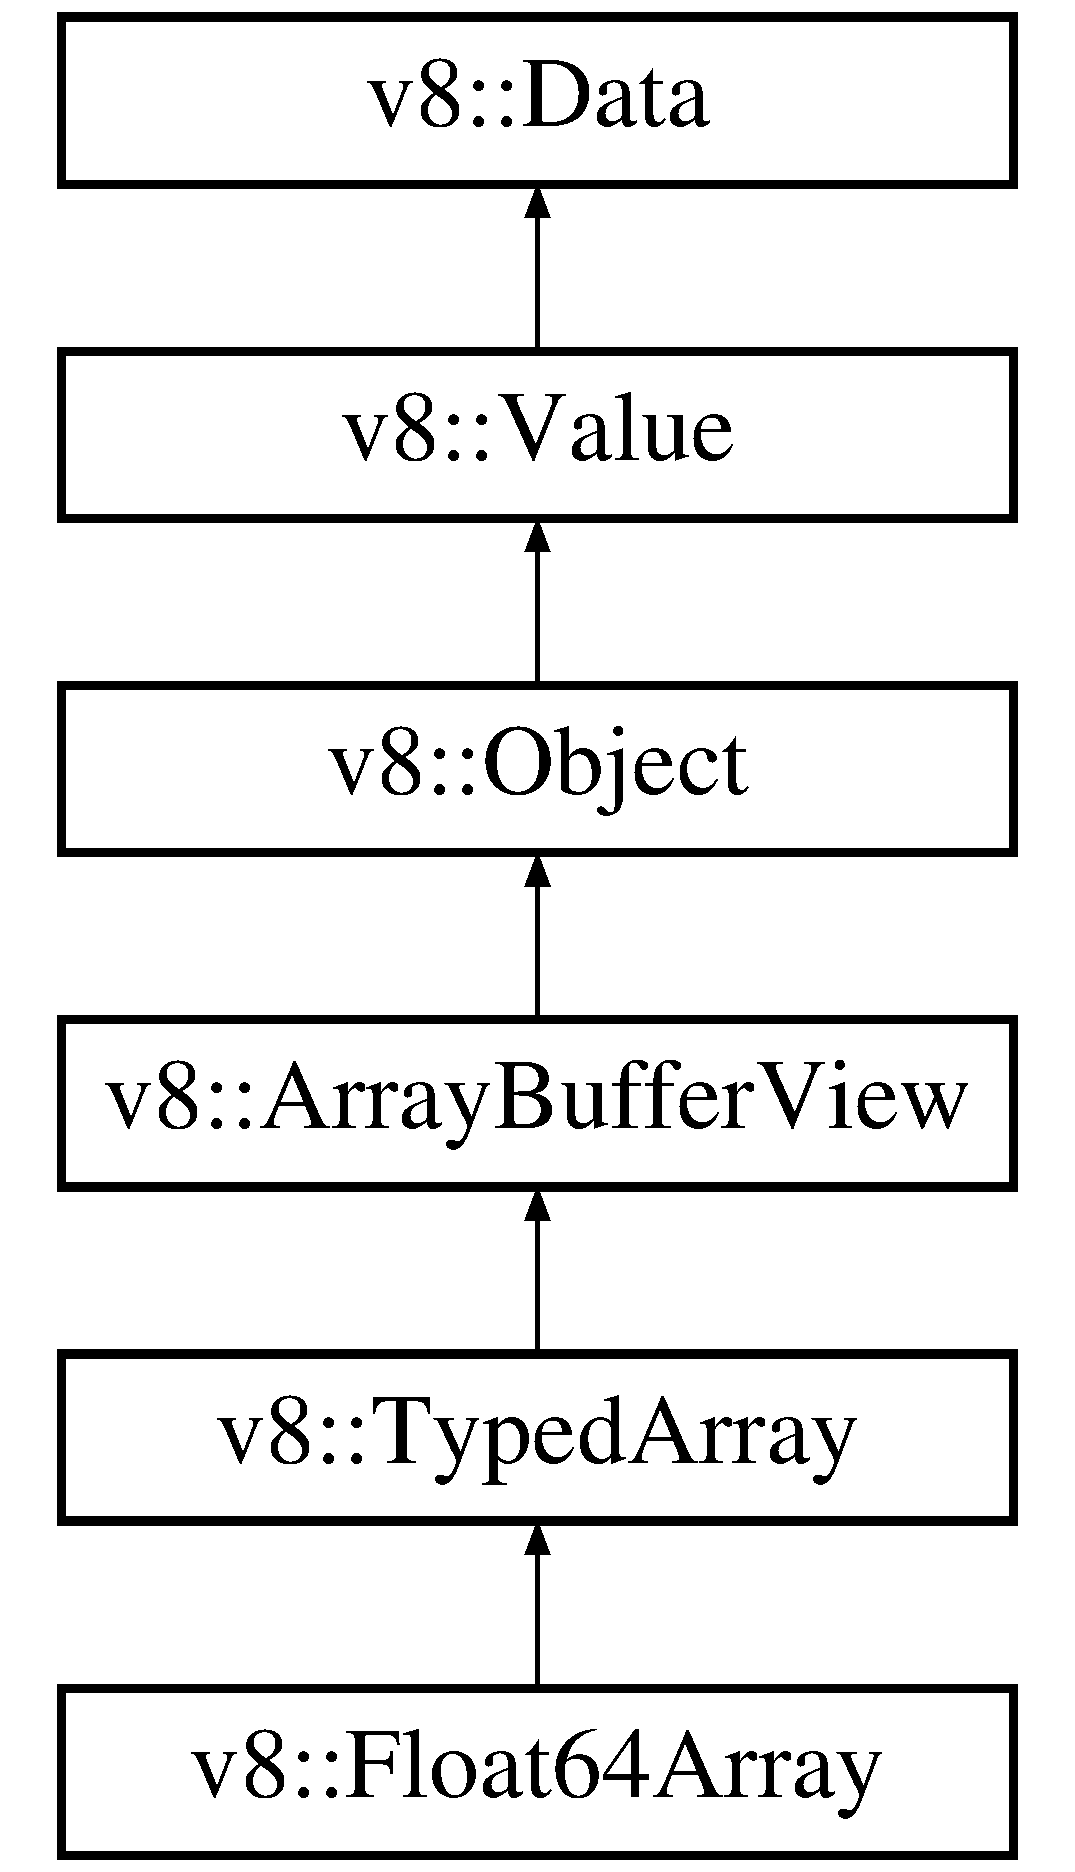
\includegraphics[height=6.000000cm]{classv8_1_1_float64_array}
\end{center}
\end{figure}
\subsection*{Static Public Member Functions}
\begin{DoxyCompactItemize}
\item 
static \hyperlink{classv8_1_1_local}{Local}$<$ \hyperlink{classv8_1_1_float64_array}{Float64\+Array} $>$ {\bfseries New} (\hyperlink{classv8_1_1_local}{Local}$<$ \hyperlink{classv8_1_1_array_buffer}{Array\+Buffer} $>$ array\+\_\+buffer, size\+\_\+t byte\+\_\+offset, size\+\_\+t length)\hypertarget{classv8_1_1_float64_array_a6e12e5ced578a357cfd049e036c4d6d6}{}\label{classv8_1_1_float64_array_a6e12e5ced578a357cfd049e036c4d6d6}

\item 
static \hyperlink{classv8_1_1_local}{Local}$<$ \hyperlink{classv8_1_1_float64_array}{Float64\+Array} $>$ {\bfseries New} (\hyperlink{classv8_1_1_local}{Local}$<$ \hyperlink{classv8_1_1_shared_array_buffer}{Shared\+Array\+Buffer} $>$ shared\+\_\+array\+\_\+buffer, size\+\_\+t byte\+\_\+offset, size\+\_\+t length)\hypertarget{classv8_1_1_float64_array_aff414a8613e468f7deb29996f049e130}{}\label{classv8_1_1_float64_array_aff414a8613e468f7deb29996f049e130}

\item 
static V8\+\_\+\+I\+N\+L\+I\+NE \hyperlink{classv8_1_1_float64_array}{Float64\+Array} $\ast$ {\bfseries Cast} (\hyperlink{classv8_1_1_value}{Value} $\ast$obj)\hypertarget{classv8_1_1_float64_array_a936ee8e8cb2cb892cc5369e3ee6a7784}{}\label{classv8_1_1_float64_array_a936ee8e8cb2cb892cc5369e3ee6a7784}

\end{DoxyCompactItemize}
\subsection*{Static Private Member Functions}
\begin{DoxyCompactItemize}
\item 
static void {\bfseries Check\+Cast} (\hyperlink{classv8_1_1_value}{Value} $\ast$obj)\hypertarget{classv8_1_1_float64_array_af351dcd287535555bca435b201ef60be}{}\label{classv8_1_1_float64_array_af351dcd287535555bca435b201ef60be}

\end{DoxyCompactItemize}
\subsection*{Additional Inherited Members}


\subsection{Detailed Description}
An instance of \hyperlink{classv8_1_1_float64_array}{Float64\+Array} constructor (E\+S6 draft 15.\+13.\+6). This A\+PI is experimental and may change significantly. 

The documentation for this class was generated from the following file\+:\begin{DoxyCompactItemize}
\item 
/\+Users/joshgav/node/v8/include/v8.\+h\end{DoxyCompactItemize}

\hypertarget{classv8_1_1_function}{}\section{v8\+:\+:Function Class Reference}
\label{classv8_1_1_function}\index{v8\+::\+Function@{v8\+::\+Function}}


{\ttfamily \#include $<$v8.\+h$>$}

Inheritance diagram for v8\+:\+:Function\+:\begin{figure}[H]
\begin{center}
\leavevmode
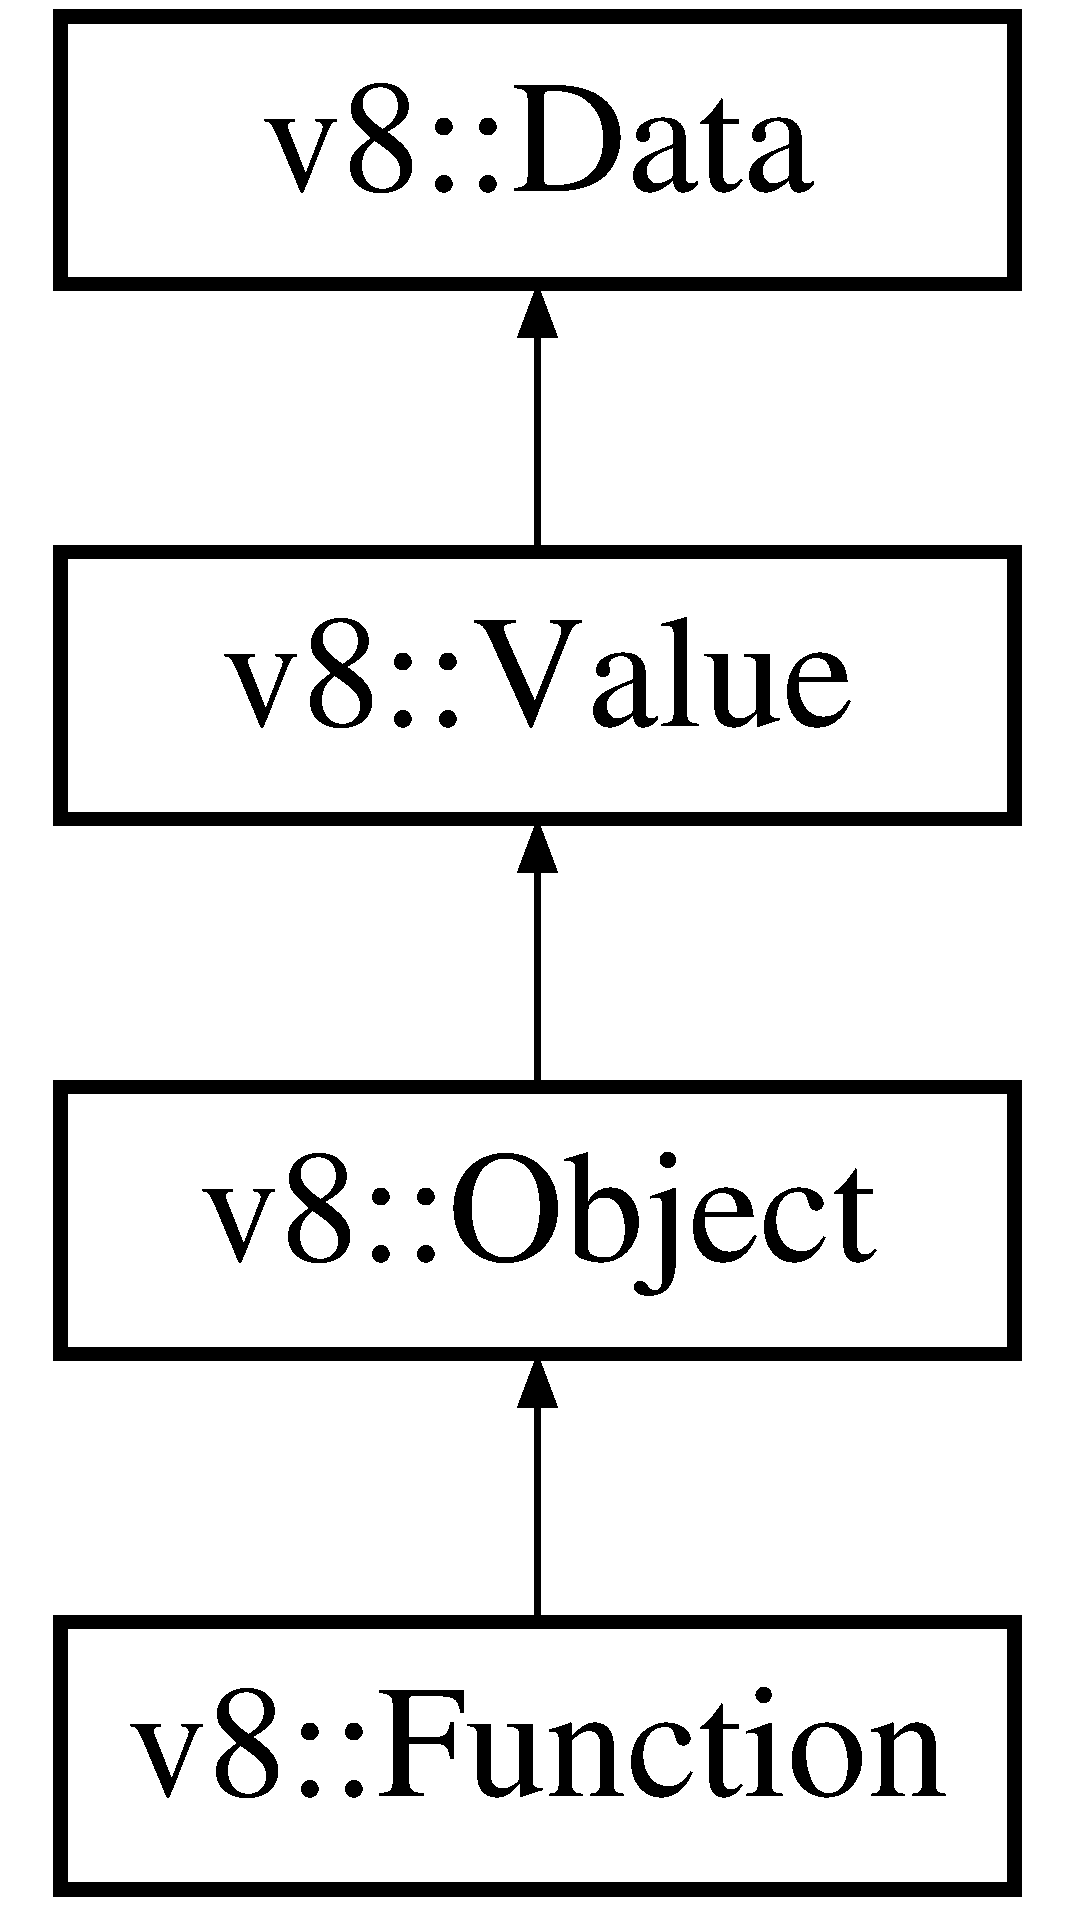
\includegraphics[height=4.000000cm]{classv8_1_1_function}
\end{center}
\end{figure}
\subsection*{Public Member Functions}
\begin{DoxyCompactItemize}
\item 
{\bfseries V8\+\_\+\+D\+E\+P\+R\+E\+C\+A\+T\+ED} (\char`\"{}Use maybe version\char`\"{}, Local$<$ \hyperlink{classv8_1_1_object}{Object} $>$ New\+Instance(int argc, \hyperlink{classv8_1_1_local}{Local}$<$ \hyperlink{classv8_1_1_value}{Value} $>$ argv\mbox{[}$\,$\mbox{]}) const)\hypertarget{classv8_1_1_function_a98095d92f7b6ae5778ac4ab88eca8411}{}\label{classv8_1_1_function_a98095d92f7b6ae5778ac4ab88eca8411}

\item 
V8\+\_\+\+W\+A\+R\+N\+\_\+\+U\+N\+U\+S\+E\+D\+\_\+\+R\+E\+S\+U\+LT \hyperlink{classv8_1_1_maybe_local}{Maybe\+Local}$<$ \hyperlink{classv8_1_1_object}{Object} $>$ {\bfseries New\+Instance} (\hyperlink{classv8_1_1_local}{Local}$<$ \hyperlink{classv8_1_1_context}{Context} $>$ context, int argc, \hyperlink{classv8_1_1_local}{Local}$<$ \hyperlink{classv8_1_1_value}{Value} $>$ argv\mbox{[}$\,$\mbox{]}) const \hypertarget{classv8_1_1_function_a32c17bdfafde9a11e4606abc09da3d58}{}\label{classv8_1_1_function_a32c17bdfafde9a11e4606abc09da3d58}

\item 
{\bfseries V8\+\_\+\+D\+E\+P\+R\+E\+C\+A\+T\+ED} (\char`\"{}Use maybe version\char`\"{}, Local$<$ \hyperlink{classv8_1_1_object}{Object} $>$ New\+Instance() const)\hypertarget{classv8_1_1_function_a120cfd8b1caaad09701c6ac0f4c2e68f}{}\label{classv8_1_1_function_a120cfd8b1caaad09701c6ac0f4c2e68f}

\item 
V8\+\_\+\+W\+A\+R\+N\+\_\+\+U\+N\+U\+S\+E\+D\+\_\+\+R\+E\+S\+U\+LT \hyperlink{classv8_1_1_maybe_local}{Maybe\+Local}$<$ \hyperlink{classv8_1_1_object}{Object} $>$ {\bfseries New\+Instance} (\hyperlink{classv8_1_1_local}{Local}$<$ \hyperlink{classv8_1_1_context}{Context} $>$ context) const \hypertarget{classv8_1_1_function_aae5c830b715559ab0d2e941ad8181cb2}{}\label{classv8_1_1_function_aae5c830b715559ab0d2e941ad8181cb2}

\item 
{\bfseries V8\+\_\+\+D\+E\+P\+R\+E\+C\+A\+T\+E\+\_\+\+S\+O\+ON} (\char`\"{}Use maybe version\char`\"{}, Local$<$ \hyperlink{classv8_1_1_value}{Value} $>$ Call(\hyperlink{classv8_1_1_local}{Local}$<$ \hyperlink{classv8_1_1_value}{Value} $>$ recv, int argc,                                                                                                                                               \hyperlink{classv8_1_1_local}{Local}$<$ \hyperlink{classv8_1_1_value}{Value} $>$ argv\mbox{[}$\,$\mbox{]}))\hypertarget{classv8_1_1_function_abb60ed7908921dcf8a57d386107a14d5}{}\label{classv8_1_1_function_abb60ed7908921dcf8a57d386107a14d5}

\item 
V8\+\_\+\+W\+A\+R\+N\+\_\+\+U\+N\+U\+S\+E\+D\+\_\+\+R\+E\+S\+U\+LT \hyperlink{classv8_1_1_maybe_local}{Maybe\+Local}$<$ \hyperlink{classv8_1_1_value}{Value} $>$ {\bfseries Call} (\hyperlink{classv8_1_1_local}{Local}$<$ \hyperlink{classv8_1_1_context}{Context} $>$ context, \hyperlink{classv8_1_1_local}{Local}$<$ \hyperlink{classv8_1_1_value}{Value} $>$ recv, int argc, \hyperlink{classv8_1_1_local}{Local}$<$ \hyperlink{classv8_1_1_value}{Value} $>$ argv\mbox{[}$\,$\mbox{]})\hypertarget{classv8_1_1_function_a8ba77d12e5716e451b32a79459cc75dd}{}\label{classv8_1_1_function_a8ba77d12e5716e451b32a79459cc75dd}

\item 
void {\bfseries Set\+Name} (\hyperlink{classv8_1_1_local}{Local}$<$ \hyperlink{classv8_1_1_string}{String} $>$ name)\hypertarget{classv8_1_1_function_aa9f51cea2036e0caa317e3955109856d}{}\label{classv8_1_1_function_aa9f51cea2036e0caa317e3955109856d}

\item 
\hyperlink{classv8_1_1_local}{Local}$<$ \hyperlink{classv8_1_1_value}{Value} $>$ {\bfseries Get\+Name} () const \hypertarget{classv8_1_1_function_a5f25cc42b8811060b94cc649dc498c7a}{}\label{classv8_1_1_function_a5f25cc42b8811060b94cc649dc498c7a}

\item 
\hyperlink{classv8_1_1_local}{Local}$<$ \hyperlink{classv8_1_1_value}{Value} $>$ \hyperlink{classv8_1_1_function_a9f888ed2c59f06ee9716c129689b60ea}{Get\+Inferred\+Name} () const 
\item 
\hyperlink{classv8_1_1_local}{Local}$<$ \hyperlink{classv8_1_1_value}{Value} $>$ \hyperlink{classv8_1_1_function_a7873d060de13cf6c336408ac75ba58fc}{Get\+Debug\+Name} () const 
\item 
\hyperlink{classv8_1_1_local}{Local}$<$ \hyperlink{classv8_1_1_value}{Value} $>$ \hyperlink{classv8_1_1_function_a87ce752e8f0451790188a62df9e9408f}{Get\+Display\+Name} () const 
\item 
int \hyperlink{classv8_1_1_function_ae64de1b9dc1ea5dc4f419a88808c12c5}{Get\+Script\+Line\+Number} () const 
\item 
int \hyperlink{classv8_1_1_function_abfe6a9251c5dfc995b83dcf3032fdc86}{Get\+Script\+Column\+Number} () const 
\item 
bool \hyperlink{classv8_1_1_function_a4279e2bfca281cda9afdaf86c87d644d}{Is\+Builtin} () const 
\item 
int \hyperlink{classv8_1_1_function_afa208e62e702f6d61ba0a4250ba3f2cf}{Script\+Id} () const 
\item 
\hyperlink{classv8_1_1_local}{Local}$<$ \hyperlink{classv8_1_1_value}{Value} $>$ \hyperlink{classv8_1_1_function_add3ee40016188aa0abf7f63cf3a3c95d}{Get\+Bound\+Function} () const 
\item 
\hyperlink{classv8_1_1_script_origin}{Script\+Origin} {\bfseries Get\+Script\+Origin} () const \hypertarget{classv8_1_1_function_af9c77c9bcbf698727071c7153e7c2513}{}\label{classv8_1_1_function_af9c77c9bcbf698727071c7153e7c2513}

\end{DoxyCompactItemize}
\subsection*{Static Public Member Functions}
\begin{DoxyCompactItemize}
\item 
static \hyperlink{classv8_1_1_maybe_local}{Maybe\+Local}$<$ \hyperlink{classv8_1_1_function}{Function} $>$ \hyperlink{classv8_1_1_function_a74b0edad0cc88a69593db0c5ae63b454}{New} (\hyperlink{classv8_1_1_local}{Local}$<$ \hyperlink{classv8_1_1_context}{Context} $>$ context, Function\+Callback callback, \hyperlink{classv8_1_1_local}{Local}$<$ \hyperlink{classv8_1_1_value}{Value} $>$ data=\hyperlink{classv8_1_1_local}{Local}$<$ \hyperlink{classv8_1_1_value}{Value} $>$(), int length=0)
\item 
static {\bfseries V8\+\_\+\+D\+E\+P\+R\+E\+C\+A\+T\+E\+\_\+\+S\+O\+ON} (\char`\"{}Use maybe version\char`\"{}, Local$<$ \hyperlink{classv8_1_1_function}{Function} $>$ \hyperlink{classv8_1_1_function_a74b0edad0cc88a69593db0c5ae63b454}{New}(\hyperlink{classv8_1_1_isolate}{Isolate} $\ast$isolate, Function\+Callback callback,                                                                                               \hyperlink{classv8_1_1_local}{Local}$<$ \hyperlink{classv8_1_1_value}{Value} $>$ data=\hyperlink{classv8_1_1_local}{Local}$<$ \hyperlink{classv8_1_1_value}{Value} $>$(), int length=0))\hypertarget{classv8_1_1_function_ac6281ad77b5f3ab414b7fd315471326d}{}\label{classv8_1_1_function_ac6281ad77b5f3ab414b7fd315471326d}

\item 
static V8\+\_\+\+I\+N\+L\+I\+NE \hyperlink{classv8_1_1_function}{Function} $\ast$ {\bfseries Cast} (\hyperlink{classv8_1_1_value}{Value} $\ast$obj)\hypertarget{classv8_1_1_function_af24f38bcc0769519816cda1f6a154ff8}{}\label{classv8_1_1_function_af24f38bcc0769519816cda1f6a154ff8}

\end{DoxyCompactItemize}
\subsection*{Static Public Attributes}
\begin{DoxyCompactItemize}
\item 
static const int {\bfseries k\+Line\+Offset\+Not\+Found} = -\/1\hypertarget{classv8_1_1_function_acf0af24f79908e405a6ac435277596d9}{}\label{classv8_1_1_function_acf0af24f79908e405a6ac435277596d9}

\end{DoxyCompactItemize}
\subsection*{Static Private Member Functions}
\begin{DoxyCompactItemize}
\item 
static void {\bfseries Check\+Cast} (\hyperlink{classv8_1_1_value}{Value} $\ast$obj)\hypertarget{classv8_1_1_function_aa2c82ea6d9fab107f803d35aa36b9193}{}\label{classv8_1_1_function_aa2c82ea6d9fab107f803d35aa36b9193}

\end{DoxyCompactItemize}


\subsection{Detailed Description}
A Java\+Script function object (E\+C\+M\+A-\/262, 15.\+3). 

\subsection{Member Function Documentation}
\index{v8\+::\+Function@{v8\+::\+Function}!Get\+Bound\+Function@{Get\+Bound\+Function}}
\index{Get\+Bound\+Function@{Get\+Bound\+Function}!v8\+::\+Function@{v8\+::\+Function}}
\subsubsection[{\texorpdfstring{Get\+Bound\+Function() const }{GetBoundFunction() const }}]{\setlength{\rightskip}{0pt plus 5cm}{\bf Local}$<$ {\bf v8\+::\+Value} $>$ v8\+::\+Function\+::\+Get\+Bound\+Function (
\begin{DoxyParamCaption}
{}
\end{DoxyParamCaption}
) const}\hypertarget{classv8_1_1_function_add3ee40016188aa0abf7f63cf3a3c95d}{}\label{classv8_1_1_function_add3ee40016188aa0abf7f63cf3a3c95d}
Returns the original function if this function is bound, else returns v8\+::\+Undefined. \index{v8\+::\+Function@{v8\+::\+Function}!Get\+Debug\+Name@{Get\+Debug\+Name}}
\index{Get\+Debug\+Name@{Get\+Debug\+Name}!v8\+::\+Function@{v8\+::\+Function}}
\subsubsection[{\texorpdfstring{Get\+Debug\+Name() const }{GetDebugName() const }}]{\setlength{\rightskip}{0pt plus 5cm}{\bf Local}$<$ {\bf Value} $>$ v8\+::\+Function\+::\+Get\+Debug\+Name (
\begin{DoxyParamCaption}
{}
\end{DoxyParamCaption}
) const}\hypertarget{classv8_1_1_function_a7873d060de13cf6c336408ac75ba58fc}{}\label{classv8_1_1_function_a7873d060de13cf6c336408ac75ba58fc}
display\+Name if it is set, otherwise name if it is configured, otherwise function name, otherwise inferred name. \index{v8\+::\+Function@{v8\+::\+Function}!Get\+Display\+Name@{Get\+Display\+Name}}
\index{Get\+Display\+Name@{Get\+Display\+Name}!v8\+::\+Function@{v8\+::\+Function}}
\subsubsection[{\texorpdfstring{Get\+Display\+Name() const }{GetDisplayName() const }}]{\setlength{\rightskip}{0pt plus 5cm}{\bf Local}$<$ {\bf Value} $>$ v8\+::\+Function\+::\+Get\+Display\+Name (
\begin{DoxyParamCaption}
{}
\end{DoxyParamCaption}
) const}\hypertarget{classv8_1_1_function_a87ce752e8f0451790188a62df9e9408f}{}\label{classv8_1_1_function_a87ce752e8f0451790188a62df9e9408f}
User-\/defined name assigned to the \char`\"{}display\+Name\char`\"{} property of this function. Used to facilitate debugging and profiling of Java\+Script code. \index{v8\+::\+Function@{v8\+::\+Function}!Get\+Inferred\+Name@{Get\+Inferred\+Name}}
\index{Get\+Inferred\+Name@{Get\+Inferred\+Name}!v8\+::\+Function@{v8\+::\+Function}}
\subsubsection[{\texorpdfstring{Get\+Inferred\+Name() const }{GetInferredName() const }}]{\setlength{\rightskip}{0pt plus 5cm}{\bf Local}$<$ {\bf Value} $>$ v8\+::\+Function\+::\+Get\+Inferred\+Name (
\begin{DoxyParamCaption}
{}
\end{DoxyParamCaption}
) const}\hypertarget{classv8_1_1_function_a9f888ed2c59f06ee9716c129689b60ea}{}\label{classv8_1_1_function_a9f888ed2c59f06ee9716c129689b60ea}
\hyperlink{classv8_1_1_name}{Name} inferred from variable or property assignment of this function. Used to facilitate debugging and profiling of Java\+Script code written in an OO style, where many functions are anonymous but are assigned to object properties. \index{v8\+::\+Function@{v8\+::\+Function}!Get\+Script\+Column\+Number@{Get\+Script\+Column\+Number}}
\index{Get\+Script\+Column\+Number@{Get\+Script\+Column\+Number}!v8\+::\+Function@{v8\+::\+Function}}
\subsubsection[{\texorpdfstring{Get\+Script\+Column\+Number() const }{GetScriptColumnNumber() const }}]{\setlength{\rightskip}{0pt plus 5cm}int v8\+::\+Function\+::\+Get\+Script\+Column\+Number (
\begin{DoxyParamCaption}
{}
\end{DoxyParamCaption}
) const}\hypertarget{classv8_1_1_function_abfe6a9251c5dfc995b83dcf3032fdc86}{}\label{classv8_1_1_function_abfe6a9251c5dfc995b83dcf3032fdc86}
Returns zero based column number of function body and k\+Line\+Offset\+Not\+Found if no information available. \index{v8\+::\+Function@{v8\+::\+Function}!Get\+Script\+Line\+Number@{Get\+Script\+Line\+Number}}
\index{Get\+Script\+Line\+Number@{Get\+Script\+Line\+Number}!v8\+::\+Function@{v8\+::\+Function}}
\subsubsection[{\texorpdfstring{Get\+Script\+Line\+Number() const }{GetScriptLineNumber() const }}]{\setlength{\rightskip}{0pt plus 5cm}int v8\+::\+Function\+::\+Get\+Script\+Line\+Number (
\begin{DoxyParamCaption}
{}
\end{DoxyParamCaption}
) const}\hypertarget{classv8_1_1_function_ae64de1b9dc1ea5dc4f419a88808c12c5}{}\label{classv8_1_1_function_ae64de1b9dc1ea5dc4f419a88808c12c5}
Returns zero based line number of function body and k\+Line\+Offset\+Not\+Found if no information available. \index{v8\+::\+Function@{v8\+::\+Function}!Is\+Builtin@{Is\+Builtin}}
\index{Is\+Builtin@{Is\+Builtin}!v8\+::\+Function@{v8\+::\+Function}}
\subsubsection[{\texorpdfstring{Is\+Builtin() const }{IsBuiltin() const }}]{\setlength{\rightskip}{0pt plus 5cm}bool v8\+::\+Function\+::\+Is\+Builtin (
\begin{DoxyParamCaption}
{}
\end{DoxyParamCaption}
) const}\hypertarget{classv8_1_1_function_a4279e2bfca281cda9afdaf86c87d644d}{}\label{classv8_1_1_function_a4279e2bfca281cda9afdaf86c87d644d}
Tells whether this function is builtin. \index{v8\+::\+Function@{v8\+::\+Function}!New@{New}}
\index{New@{New}!v8\+::\+Function@{v8\+::\+Function}}
\subsubsection[{\texorpdfstring{New(\+Local$<$ Context $>$ context, Function\+Callback callback, Local$<$ Value $>$ data=\+Local$<$ Value $>$(), int length=0)}{New(Local< Context > context, FunctionCallback callback, Local< Value > data=Local< Value >(), int length=0)}}]{\setlength{\rightskip}{0pt plus 5cm}{\bf Local}$<$ {\bf Function} $>$ v8\+::\+Function\+::\+New (
\begin{DoxyParamCaption}
\item[{{\bf Local}$<$ {\bf Context} $>$}]{context, }
\item[{Function\+Callback}]{callback, }
\item[{{\bf Local}$<$ {\bf Value} $>$}]{data = {\ttfamily {\bf Local}$<${\bf Value}$>$()}, }
\item[{int}]{length = {\ttfamily 0}}
\end{DoxyParamCaption}
)\hspace{0.3cm}{\ttfamily [static]}}\hypertarget{classv8_1_1_function_a74b0edad0cc88a69593db0c5ae63b454}{}\label{classv8_1_1_function_a74b0edad0cc88a69593db0c5ae63b454}
Create a function in the current execution context for a given Function\+Callback. \index{v8\+::\+Function@{v8\+::\+Function}!Script\+Id@{Script\+Id}}
\index{Script\+Id@{Script\+Id}!v8\+::\+Function@{v8\+::\+Function}}
\subsubsection[{\texorpdfstring{Script\+Id() const }{ScriptId() const }}]{\setlength{\rightskip}{0pt plus 5cm}int v8\+::\+Function\+::\+Script\+Id (
\begin{DoxyParamCaption}
{}
\end{DoxyParamCaption}
) const}\hypertarget{classv8_1_1_function_afa208e62e702f6d61ba0a4250ba3f2cf}{}\label{classv8_1_1_function_afa208e62e702f6d61ba0a4250ba3f2cf}
Returns script\+Id. 

The documentation for this class was generated from the following files\+:\begin{DoxyCompactItemize}
\item 
/\+Users/joshgav/node/v8/include/v8.\+h\item 
/\+Users/joshgav/node/v8/src/api.\+cc\end{DoxyCompactItemize}

\hypertarget{classv8_1_1_function_callback_info}{}\section{v8\+:\+:Function\+Callback\+Info$<$ T $>$ Class Template Reference}
\label{classv8_1_1_function_callback_info}\index{v8\+::\+Function\+Callback\+Info$<$ T $>$@{v8\+::\+Function\+Callback\+Info$<$ T $>$}}


{\ttfamily \#include $<$v8.\+h$>$}

\subsection*{Public Member Functions}
\begin{DoxyCompactItemize}
\item 
V8\+\_\+\+I\+N\+L\+I\+NE int {\bfseries Length} () const \hypertarget{classv8_1_1_function_callback_info_ab27e070d5dca1974adcd1ff9e5482c6e}{}\label{classv8_1_1_function_callback_info_ab27e070d5dca1974adcd1ff9e5482c6e}

\item 
V8\+\_\+\+I\+N\+L\+I\+NE \hyperlink{classv8_1_1_local}{Local}$<$ \hyperlink{classv8_1_1_value}{Value} $>$ {\bfseries operator\mbox{[}$\,$\mbox{]}} (int i) const \hypertarget{classv8_1_1_function_callback_info_a0d911f2ef4a2afcb9a29fbae9e733d9b}{}\label{classv8_1_1_function_callback_info_a0d911f2ef4a2afcb9a29fbae9e733d9b}

\item 
V8\+\_\+\+I\+N\+L\+I\+NE {\bfseries V8\+\_\+\+D\+E\+P\+R\+E\+C\+A\+T\+ED} (\char`\"{}Use \hyperlink{classv8_1_1_data}{Data}() to explicitly pass Callee instead\char`\"{}, Local$<$ \hyperlink{classv8_1_1_function}{Function} $>$ Callee() const)\hypertarget{classv8_1_1_function_callback_info_ab7f9c2a3b7c47d99df6c0f700ae7c1db}{}\label{classv8_1_1_function_callback_info_ab7f9c2a3b7c47d99df6c0f700ae7c1db}

\item 
V8\+\_\+\+I\+N\+L\+I\+NE \hyperlink{classv8_1_1_local}{Local}$<$ \hyperlink{classv8_1_1_object}{Object} $>$ {\bfseries This} () const \hypertarget{classv8_1_1_function_callback_info_a14c7f2df117ad879df898f8451a3fa38}{}\label{classv8_1_1_function_callback_info_a14c7f2df117ad879df898f8451a3fa38}

\item 
V8\+\_\+\+I\+N\+L\+I\+NE \hyperlink{classv8_1_1_local}{Local}$<$ \hyperlink{classv8_1_1_object}{Object} $>$ {\bfseries Holder} () const \hypertarget{classv8_1_1_function_callback_info_a5b080ddb61501773dfd32058b26a5238}{}\label{classv8_1_1_function_callback_info_a5b080ddb61501773dfd32058b26a5238}

\item 
V8\+\_\+\+I\+N\+L\+I\+NE \hyperlink{classv8_1_1_local}{Local}$<$ \hyperlink{classv8_1_1_value}{Value} $>$ {\bfseries New\+Target} () const \hypertarget{classv8_1_1_function_callback_info_a11cd0cd24b181bc6d39c3d0e203c2eee}{}\label{classv8_1_1_function_callback_info_a11cd0cd24b181bc6d39c3d0e203c2eee}

\item 
V8\+\_\+\+I\+N\+L\+I\+NE bool {\bfseries Is\+Construct\+Call} () const \hypertarget{classv8_1_1_function_callback_info_a8b89715c355b707efd3d2bcf21e64d9e}{}\label{classv8_1_1_function_callback_info_a8b89715c355b707efd3d2bcf21e64d9e}

\item 
V8\+\_\+\+I\+N\+L\+I\+NE \hyperlink{classv8_1_1_local}{Local}$<$ \hyperlink{classv8_1_1_value}{Value} $>$ {\bfseries Data} () const \hypertarget{classv8_1_1_function_callback_info_a1475dcc776c8fdd68eb1be08cd29e5ac}{}\label{classv8_1_1_function_callback_info_a1475dcc776c8fdd68eb1be08cd29e5ac}

\item 
V8\+\_\+\+I\+N\+L\+I\+NE \hyperlink{classv8_1_1_isolate}{Isolate} $\ast$ {\bfseries Get\+Isolate} () const \hypertarget{classv8_1_1_function_callback_info_a3b5fe01205c99dca06e388c3d390a40e}{}\label{classv8_1_1_function_callback_info_a3b5fe01205c99dca06e388c3d390a40e}

\item 
V8\+\_\+\+I\+N\+L\+I\+NE \hyperlink{classv8_1_1_return_value}{Return\+Value}$<$ T $>$ {\bfseries Get\+Return\+Value} () const \hypertarget{classv8_1_1_function_callback_info_abf851b51557b0507ab69c494fddbb3c3}{}\label{classv8_1_1_function_callback_info_abf851b51557b0507ab69c494fddbb3c3}

\end{DoxyCompactItemize}
\subsection*{Static Public Attributes}
\begin{DoxyCompactItemize}
\item 
static const int {\bfseries k\+Args\+Length} = 8\hypertarget{classv8_1_1_function_callback_info_a1e5248c2d40840270829882feaaa9d34}{}\label{classv8_1_1_function_callback_info_a1e5248c2d40840270829882feaaa9d34}

\end{DoxyCompactItemize}
\subsection*{Protected Member Functions}
\begin{DoxyCompactItemize}
\item 
V8\+\_\+\+I\+N\+L\+I\+NE {\bfseries Function\+Callback\+Info} (internal\+::\+Object $\ast$$\ast$implicit\+\_\+args, internal\+::\+Object $\ast$$\ast$values, int length)\hypertarget{classv8_1_1_function_callback_info_ad479ef760ed88d4354c267d2068deaca}{}\label{classv8_1_1_function_callback_info_ad479ef760ed88d4354c267d2068deaca}

\end{DoxyCompactItemize}
\subsection*{Protected Attributes}
\begin{DoxyCompactItemize}
\item 
internal\+::\+Object $\ast$$\ast$ {\bfseries implicit\+\_\+args\+\_\+}\hypertarget{classv8_1_1_function_callback_info_ab8a2c77ae9ea4f1406c4e488c7cdd700}{}\label{classv8_1_1_function_callback_info_ab8a2c77ae9ea4f1406c4e488c7cdd700}

\item 
internal\+::\+Object $\ast$$\ast$ {\bfseries values\+\_\+}\hypertarget{classv8_1_1_function_callback_info_a21b29295968c0797c9f94ab6c7f571ca}{}\label{classv8_1_1_function_callback_info_a21b29295968c0797c9f94ab6c7f571ca}

\item 
int {\bfseries length\+\_\+}\hypertarget{classv8_1_1_function_callback_info_ab250ace06b495beb6f14b192eff77005}{}\label{classv8_1_1_function_callback_info_ab250ace06b495beb6f14b192eff77005}

\end{DoxyCompactItemize}
\subsection*{Static Protected Attributes}
\begin{DoxyCompactItemize}
\item 
static const int {\bfseries k\+Holder\+Index} = 0\hypertarget{classv8_1_1_function_callback_info_a073824921daf8600fb9c00c50ee8ef0c}{}\label{classv8_1_1_function_callback_info_a073824921daf8600fb9c00c50ee8ef0c}

\item 
static const int {\bfseries k\+Isolate\+Index} = 1\hypertarget{classv8_1_1_function_callback_info_a0e2fbe5a323276263c848ea8050a34eb}{}\label{classv8_1_1_function_callback_info_a0e2fbe5a323276263c848ea8050a34eb}

\item 
static const int {\bfseries k\+Return\+Value\+Default\+Value\+Index} = 2\hypertarget{classv8_1_1_function_callback_info_a0b32b5613fe2f0cd139d9dffc0916d09}{}\label{classv8_1_1_function_callback_info_a0b32b5613fe2f0cd139d9dffc0916d09}

\item 
static const int {\bfseries k\+Return\+Value\+Index} = 3\hypertarget{classv8_1_1_function_callback_info_abb339e201184ebe2502a1202d54201ca}{}\label{classv8_1_1_function_callback_info_abb339e201184ebe2502a1202d54201ca}

\item 
static const int {\bfseries k\+Data\+Index} = 4\hypertarget{classv8_1_1_function_callback_info_a152c34c5b2f8c55d04d6d541bf8a4544}{}\label{classv8_1_1_function_callback_info_a152c34c5b2f8c55d04d6d541bf8a4544}

\item 
static const int {\bfseries k\+Callee\+Index} = 5\hypertarget{classv8_1_1_function_callback_info_a08a4ef2004bfaa468df347d357849ca6}{}\label{classv8_1_1_function_callback_info_a08a4ef2004bfaa468df347d357849ca6}

\item 
static const int {\bfseries k\+Context\+Save\+Index} = 6\hypertarget{classv8_1_1_function_callback_info_a9c0fdcc74eea99d8fa74460086e3b80a}{}\label{classv8_1_1_function_callback_info_a9c0fdcc74eea99d8fa74460086e3b80a}

\item 
static const int {\bfseries k\+New\+Target\+Index} = 7\hypertarget{classv8_1_1_function_callback_info_a23e70f4737b7e205dc91b972d75fbd9c}{}\label{classv8_1_1_function_callback_info_a23e70f4737b7e205dc91b972d75fbd9c}

\end{DoxyCompactItemize}
\subsection*{Friends}
\begin{DoxyCompactItemize}
\item 
class {\bfseries internal\+::\+Function\+Callback\+Arguments}\hypertarget{classv8_1_1_function_callback_info_aac7268b20857fd75b69b86ded46d0f34}{}\label{classv8_1_1_function_callback_info_aac7268b20857fd75b69b86ded46d0f34}

\item 
class {\bfseries internal\+::\+Custom\+Arguments$<$ Function\+Callback\+Info $>$}\hypertarget{classv8_1_1_function_callback_info_a02d869d89b14ddd1717429c2106f955a}{}\label{classv8_1_1_function_callback_info_a02d869d89b14ddd1717429c2106f955a}

\end{DoxyCompactItemize}


\subsection{Detailed Description}
\subsubsection*{template$<$typename T$>$\\*
class v8\+::\+Function\+Callback\+Info$<$ T $>$}

The argument information given to function call callbacks. This class provides access to information about the context of the call, including the receiver, the number and values of arguments, and the holder of the function. 

The documentation for this class was generated from the following file\+:\begin{DoxyCompactItemize}
\item 
include/v8.\+h\end{DoxyCompactItemize}

\hypertarget{classv8_1_1_function_template}{}\section{v8\+:\+:Function\+Template Class Reference}
\label{classv8_1_1_function_template}\index{v8\+::\+Function\+Template@{v8\+::\+Function\+Template}}


{\ttfamily \#include $<$v8.\+h$>$}

Inheritance diagram for v8\+:\+:Function\+Template\+:\begin{figure}[H]
\begin{center}
\leavevmode
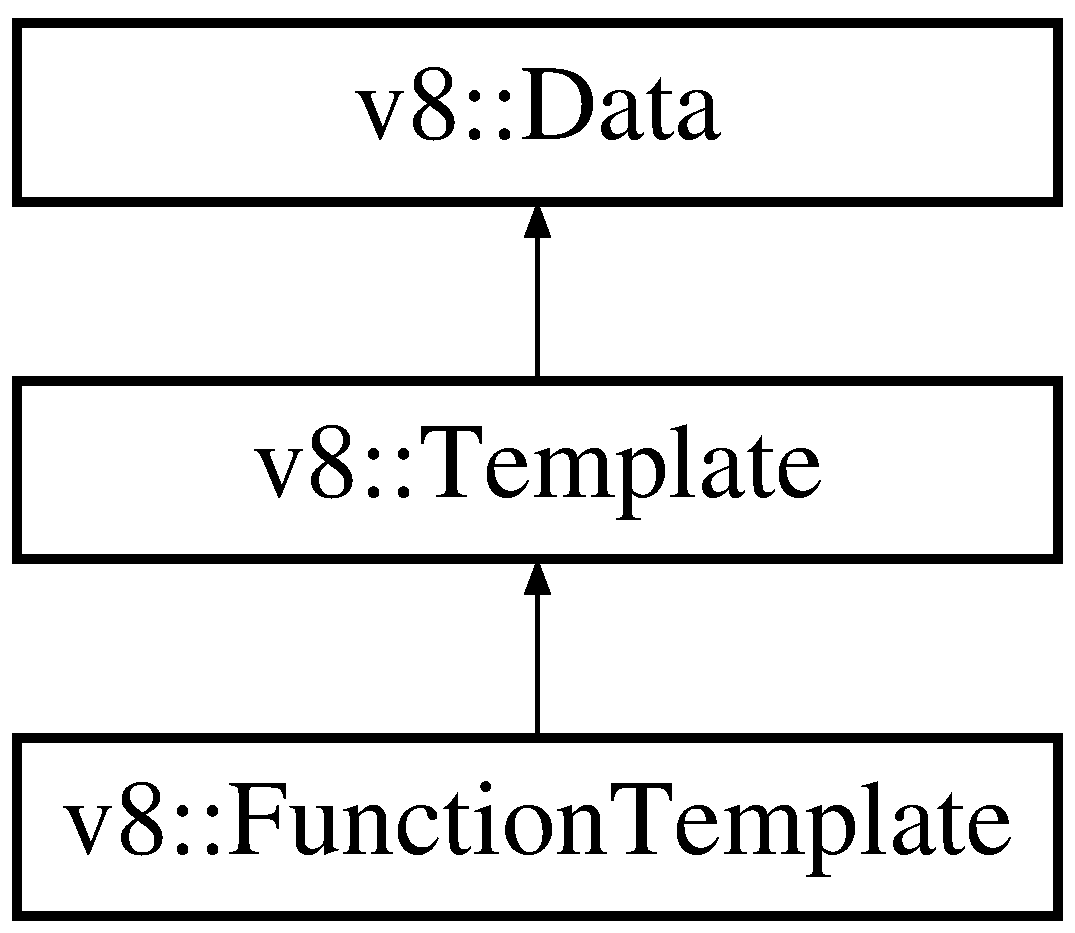
\includegraphics[height=3.000000cm]{classv8_1_1_function_template}
\end{center}
\end{figure}
\subsection*{Public Member Functions}
\begin{DoxyCompactItemize}
\item 
\hyperlink{classv8_1_1_function_template_a007fd05a3fa3c960bf7ddbc05c724d2b}{V8\+\_\+\+D\+E\+P\+R\+E\+C\+A\+T\+E\+\_\+\+S\+O\+ON} (\char`\"{}Use maybe version\char`\"{}, Local$<$ \hyperlink{classv8_1_1_function}{Function} $>$ Get\+Function())
\item 
V8\+\_\+\+W\+A\+R\+N\+\_\+\+U\+N\+U\+S\+E\+D\+\_\+\+R\+E\+S\+U\+LT \hyperlink{classv8_1_1_maybe_local}{Maybe\+Local}$<$ \hyperlink{classv8_1_1_function}{Function} $>$ {\bfseries Get\+Function} (\hyperlink{classv8_1_1_local}{Local}$<$ \hyperlink{classv8_1_1_context}{Context} $>$ context)\hypertarget{classv8_1_1_function_template_a77aa424e4ed297452be0412930340262}{}\label{classv8_1_1_function_template_a77aa424e4ed297452be0412930340262}

\item 
void \hyperlink{classv8_1_1_function_template_a3397f180b72a667ae64b31a3b371d574}{Set\+Call\+Handler} (Function\+Callback callback, \hyperlink{classv8_1_1_local}{Local}$<$ \hyperlink{classv8_1_1_value}{Value} $>$ data=\hyperlink{classv8_1_1_local}{Local}$<$ \hyperlink{classv8_1_1_value}{Value} $>$(), \hyperlink{classv8_1_1experimental_1_1_fast_accessor_builder}{experimental\+::\+Fast\+Accessor\+Builder} $\ast$fast\+\_\+handler=nullptr)
\item 
void \hyperlink{classv8_1_1_function_template_a5faf23b28ee3480b23ce054d0f389a75}{Set\+Length} (int length)
\item 
\hyperlink{classv8_1_1_local}{Local}$<$ \hyperlink{classv8_1_1_object_template}{Object\+Template} $>$ \hyperlink{classv8_1_1_function_template_a00dd9725566908e8fd14064542f5a781}{Instance\+Template} ()
\item 
void \hyperlink{classv8_1_1_function_template_abc11c462facf11bafd541892815c5425}{Inherit} (\hyperlink{classv8_1_1_local}{Local}$<$ \hyperlink{classv8_1_1_function_template}{Function\+Template} $>$ parent)
\item 
\hyperlink{classv8_1_1_local}{Local}$<$ \hyperlink{classv8_1_1_object_template}{Object\+Template} $>$ \hyperlink{classv8_1_1_function_template_aa2bcc2652b5f0fdbc666d943ccf72021}{Prototype\+Template} ()
\item 
void \hyperlink{classv8_1_1_function_template_a491e77dc7ceb5b0fe75880d11f2dbe9e}{Set\+Class\+Name} (\hyperlink{classv8_1_1_local}{Local}$<$ \hyperlink{classv8_1_1_string}{String} $>$ name)
\item 
void \hyperlink{classv8_1_1_function_template_a5ffdc68d8035b02ed7583950b76ef91f}{Set\+Accept\+Any\+Receiver} (bool value)
\item 
void \hyperlink{classv8_1_1_function_template_ade426e8a21d777ae6100e6c1aa7bfaee}{Set\+Hidden\+Prototype} (bool value)
\item 
void \hyperlink{classv8_1_1_function_template_a91d2e0643e8c5a53ab1d75f7766c2422}{Read\+Only\+Prototype} ()
\item 
void \hyperlink{classv8_1_1_function_template_a4a184aca244174c7fe52d58871d3129e}{Remove\+Prototype} ()
\item 
bool \hyperlink{classv8_1_1_function_template_a90d838f3456d300bd19d2a2cb98645bd}{Has\+Instance} (\hyperlink{classv8_1_1_local}{Local}$<$ \hyperlink{classv8_1_1_value}{Value} $>$ object)
\end{DoxyCompactItemize}
\subsection*{Static Public Member Functions}
\begin{DoxyCompactItemize}
\item 
static \hyperlink{classv8_1_1_local}{Local}$<$ \hyperlink{classv8_1_1_function_template}{Function\+Template} $>$ \hyperlink{classv8_1_1_function_template_a3c6a525ee4e0d72afa77be8e34861f83}{New} (\hyperlink{classv8_1_1_isolate}{Isolate} $\ast$isolate, Function\+Callback callback=0, \hyperlink{classv8_1_1_local}{Local}$<$ \hyperlink{classv8_1_1_value}{Value} $>$ data=\hyperlink{classv8_1_1_local}{Local}$<$ \hyperlink{classv8_1_1_value}{Value} $>$(), \hyperlink{classv8_1_1_local}{Local}$<$ \hyperlink{classv8_1_1_signature}{Signature} $>$ signature=\hyperlink{classv8_1_1_local}{Local}$<$ \hyperlink{classv8_1_1_signature}{Signature} $>$(), int length=0)
\item 
static \hyperlink{classv8_1_1_local}{Local}$<$ \hyperlink{classv8_1_1_function_template}{Function\+Template} $>$ \hyperlink{classv8_1_1_function_template_a4563d3c4a5e80c5c4dcc4f4cf8e382a4}{New\+With\+Fast\+Handler} (\hyperlink{classv8_1_1_isolate}{Isolate} $\ast$isolate, Function\+Callback callback, \hyperlink{classv8_1_1experimental_1_1_fast_accessor_builder}{experimental\+::\+Fast\+Accessor\+Builder} $\ast$fast\+\_\+handler=nullptr, \hyperlink{classv8_1_1_local}{Local}$<$ \hyperlink{classv8_1_1_value}{Value} $>$ data=\hyperlink{classv8_1_1_local}{Local}$<$ \hyperlink{classv8_1_1_value}{Value} $>$(), \hyperlink{classv8_1_1_local}{Local}$<$ \hyperlink{classv8_1_1_signature}{Signature} $>$ signature=\hyperlink{classv8_1_1_local}{Local}$<$ \hyperlink{classv8_1_1_signature}{Signature} $>$(), int length=0)
\end{DoxyCompactItemize}
\subsection*{Friends}
\begin{DoxyCompactItemize}
\item 
class {\bfseries Context}\hypertarget{classv8_1_1_function_template_ac26c806e60ca4a0547680edb68f6e39b}{}\label{classv8_1_1_function_template_ac26c806e60ca4a0547680edb68f6e39b}

\item 
class {\bfseries Object\+Template}\hypertarget{classv8_1_1_function_template_a4d28646409234f556983be8a96c06424}{}\label{classv8_1_1_function_template_a4d28646409234f556983be8a96c06424}

\end{DoxyCompactItemize}


\subsection{Detailed Description}
A \hyperlink{classv8_1_1_function_template}{Function\+Template} is used to create functions at runtime. There can only be one function created from a \hyperlink{classv8_1_1_function_template}{Function\+Template} in a context. The lifetime of the created function is equal to the lifetime of the context. So in case the embedder needs to create temporary functions that can be collected using Scripts is preferred.

Any modification of a \hyperlink{classv8_1_1_function_template}{Function\+Template} after first instantiation will trigger a crash.

A \hyperlink{classv8_1_1_function_template}{Function\+Template} can have properties, these properties are added to the function object when it is created.

A \hyperlink{classv8_1_1_function_template}{Function\+Template} has a corresponding instance template which is used to create object instances when the function is used as a constructor. Properties added to the instance template are added to each object instance.

A \hyperlink{classv8_1_1_function_template}{Function\+Template} can have a prototype template. The prototype template is used to create the prototype object of the function.

The following example shows how to use a \hyperlink{classv8_1_1_function_template}{Function\+Template}\+:


\begin{DoxyCode}
\hyperlink{classv8_1_1_local}{v8::Local<v8::FunctionTemplate>} t = 
      \hyperlink{classv8_1_1_function_template_a3c6a525ee4e0d72afa77be8e34861f83}{v8::FunctionTemplate::New}();
t->\hyperlink{classv8_1_1_template_a623b9f0cdd87dc861516f276cc9a7cfa}{Set}(\textcolor{stringliteral}{"func\_property"}, v8::Number::New(1));

\hyperlink{classv8_1_1_local}{v8::Local<v8::Template>} proto\_t = t->\hyperlink{classv8_1_1_function_template_aa2bcc2652b5f0fdbc666d943ccf72021}{PrototypeTemplate}();
proto\_t->\hyperlink{classv8_1_1_template_a623b9f0cdd87dc861516f276cc9a7cfa}{Set}(\textcolor{stringliteral}{"proto\_method"}, \hyperlink{classv8_1_1_function_template_a3c6a525ee4e0d72afa77be8e34861f83}{v8::FunctionTemplate::New}(InvokeCallback));
proto\_t->\hyperlink{classv8_1_1_template_a623b9f0cdd87dc861516f276cc9a7cfa}{Set}(\textcolor{stringliteral}{"proto\_const"}, v8::Number::New(2));

\hyperlink{classv8_1_1_local}{v8::Local<v8::ObjectTemplate>} instance\_t = t->
      \hyperlink{classv8_1_1_function_template_a00dd9725566908e8fd14064542f5a781}{InstanceTemplate}();
instance\_t->\hyperlink{classv8_1_1_object_template_a7300126e15ff8246813e07f92d4fbe83}{SetAccessor}(\textcolor{stringliteral}{"instance\_accessor"}, InstanceAccessorCallback);
instance\_t->\hyperlink{classv8_1_1_object_template_a66fa7b04c87676e20e35497ea09a0ad0}{SetNamedPropertyHandler}(PropertyHandlerCallback, ...);
instance\_t->\hyperlink{classv8_1_1_template_a623b9f0cdd87dc861516f276cc9a7cfa}{Set}(\textcolor{stringliteral}{"instance\_property"}, Number::New(3));

\hyperlink{classv8_1_1_local}{v8::Local<v8::Function>} \textcolor{keyword}{function} = t->GetFunction();
\hyperlink{classv8_1_1_local}{v8::Local<v8::Object>} instance = \textcolor{keyword}{function}->NewInstance();
\end{DoxyCode}


Let\textquotesingle{}s use \char`\"{}function\char`\"{} as the JS variable name of the function object and \char`\"{}instance\char`\"{} for the instance object created above. The function and the instance will have the following properties\+:


\begin{DoxyCode}
func\_property in \textcolor{keyword}{function} == \textcolor{keyword}{true};
\textcolor{keyword}{function}.func\_property == 1;

\textcolor{keyword}{function}.prototype.proto\_method() invokes \textcolor{stringliteral}{'InvokeCallback'}
\textcolor{keyword}{function}.prototype.proto\_const == 2;

instance instanceof \textcolor{keyword}{function} == \textcolor{keyword}{true};
instance.instance\_accessor calls \textcolor{stringliteral}{'InstanceAccessorCallback'}
instance.instance\_property == 3;
\end{DoxyCode}


A \hyperlink{classv8_1_1_function_template}{Function\+Template} can inherit from another one by calling the \hyperlink{classv8_1_1_function_template_abc11c462facf11bafd541892815c5425}{Function\+Template\+::\+Inherit} method. The following graph illustrates the semantics of inheritance\+:


\begin{DoxyCode}
FunctionTemplate Parent  -> Parent() . prototype -> \{ \}
  ^                                                  ^
  | \hyperlink{classv8_1_1_function_template_abc11c462facf11bafd541892815c5425}{Inherit}(Parent)                                  | .\_\_proto\_\_
  |                                                  |
FunctionTemplate Child   -> Child()  . prototype -> \{ \}
\end{DoxyCode}


A \hyperlink{classv8_1_1_function_template}{Function\+Template} \textquotesingle{}Child\textquotesingle{} inherits from \textquotesingle{}Parent\textquotesingle{}, the prototype object of the Child() function has {\bfseries proto} pointing to the Parent() function\textquotesingle{}s prototype object. An instance of the Child function has all properties on Parent\textquotesingle{}s instance templates.

Let Parent be the \hyperlink{classv8_1_1_function_template}{Function\+Template} initialized in the previous section and create a Child \hyperlink{classv8_1_1_function_template}{Function\+Template} by\+:


\begin{DoxyCode}
Local<FunctionTemplate> parent = t;
Local<FunctionTemplate> child = \hyperlink{classv8_1_1_function_template_a3c6a525ee4e0d72afa77be8e34861f83}{FunctionTemplate::New}();
child->Inherit(parent);

Local<Function> child\_function = child->GetFunction();
Local<Object> child\_instance = child\_function->NewInstance();
\end{DoxyCode}


The Child function and Child instance will have the following properties\+:


\begin{DoxyCode}
child\_func.prototype.\_\_proto\_\_ == \textcolor{keyword}{function}.prototype;
child\_instance.instance\_accessor calls \textcolor{stringliteral}{'InstanceAccessorCallback'}
child\_instance.instance\_property == 3;
\end{DoxyCode}
 

\subsection{Member Function Documentation}
\index{v8\+::\+Function\+Template@{v8\+::\+Function\+Template}!Has\+Instance@{Has\+Instance}}
\index{Has\+Instance@{Has\+Instance}!v8\+::\+Function\+Template@{v8\+::\+Function\+Template}}
\subsubsection[{\texorpdfstring{Has\+Instance(\+Local$<$ Value $>$ object)}{HasInstance(Local< Value > object)}}]{\setlength{\rightskip}{0pt plus 5cm}bool v8\+::\+Function\+Template\+::\+Has\+Instance (
\begin{DoxyParamCaption}
\item[{{\bf Local}$<$ {\bf Value} $>$}]{object}
\end{DoxyParamCaption}
)}\hypertarget{classv8_1_1_function_template_a90d838f3456d300bd19d2a2cb98645bd}{}\label{classv8_1_1_function_template_a90d838f3456d300bd19d2a2cb98645bd}
Returns true if the given object is an instance of this function template. \index{v8\+::\+Function\+Template@{v8\+::\+Function\+Template}!Inherit@{Inherit}}
\index{Inherit@{Inherit}!v8\+::\+Function\+Template@{v8\+::\+Function\+Template}}
\subsubsection[{\texorpdfstring{Inherit(\+Local$<$ Function\+Template $>$ parent)}{Inherit(Local< FunctionTemplate > parent)}}]{\setlength{\rightskip}{0pt plus 5cm}void v8\+::\+Function\+Template\+::\+Inherit (
\begin{DoxyParamCaption}
\item[{{\bf Local}$<$ {\bf Function\+Template} $>$}]{parent}
\end{DoxyParamCaption}
)}\hypertarget{classv8_1_1_function_template_abc11c462facf11bafd541892815c5425}{}\label{classv8_1_1_function_template_abc11c462facf11bafd541892815c5425}
Causes the function template to inherit from a parent function template. \index{v8\+::\+Function\+Template@{v8\+::\+Function\+Template}!Instance\+Template@{Instance\+Template}}
\index{Instance\+Template@{Instance\+Template}!v8\+::\+Function\+Template@{v8\+::\+Function\+Template}}
\subsubsection[{\texorpdfstring{Instance\+Template()}{InstanceTemplate()}}]{\setlength{\rightskip}{0pt plus 5cm}{\bf Local}$<${\bf Object\+Template}$>$ v8\+::\+Function\+Template\+::\+Instance\+Template (
\begin{DoxyParamCaption}
{}
\end{DoxyParamCaption}
)}\hypertarget{classv8_1_1_function_template_a00dd9725566908e8fd14064542f5a781}{}\label{classv8_1_1_function_template_a00dd9725566908e8fd14064542f5a781}
Get the Instance\+Template. \index{v8\+::\+Function\+Template@{v8\+::\+Function\+Template}!New@{New}}
\index{New@{New}!v8\+::\+Function\+Template@{v8\+::\+Function\+Template}}
\subsubsection[{\texorpdfstring{New(\+Isolate $\ast$isolate, Function\+Callback callback=0, Local$<$ Value $>$ data=\+Local$<$ Value $>$(), Local$<$ Signature $>$ signature=\+Local$<$ Signature $>$(), int length=0)}{New(Isolate *isolate, FunctionCallback callback=0, Local< Value > data=Local< Value >(), Local< Signature > signature=Local< Signature >(), int length=0)}}]{\setlength{\rightskip}{0pt plus 5cm}static {\bf Local}$<${\bf Function\+Template}$>$ v8\+::\+Function\+Template\+::\+New (
\begin{DoxyParamCaption}
\item[{{\bf Isolate} $\ast$}]{isolate, }
\item[{Function\+Callback}]{callback = {\ttfamily 0}, }
\item[{{\bf Local}$<$ {\bf Value} $>$}]{data = {\ttfamily {\bf Local}$<$~{\bf Value}~$>$()}, }
\item[{{\bf Local}$<$ {\bf Signature} $>$}]{signature = {\ttfamily {\bf Local}$<$~{\bf Signature}~$>$()}, }
\item[{int}]{length = {\ttfamily 0}}
\end{DoxyParamCaption}
)\hspace{0.3cm}{\ttfamily [static]}}\hypertarget{classv8_1_1_function_template_a3c6a525ee4e0d72afa77be8e34861f83}{}\label{classv8_1_1_function_template_a3c6a525ee4e0d72afa77be8e34861f83}
Creates a function template. \index{v8\+::\+Function\+Template@{v8\+::\+Function\+Template}!New\+With\+Fast\+Handler@{New\+With\+Fast\+Handler}}
\index{New\+With\+Fast\+Handler@{New\+With\+Fast\+Handler}!v8\+::\+Function\+Template@{v8\+::\+Function\+Template}}
\subsubsection[{\texorpdfstring{New\+With\+Fast\+Handler(\+Isolate $\ast$isolate, Function\+Callback callback, experimental\+::\+Fast\+Accessor\+Builder $\ast$fast\+\_\+handler=nullptr, Local$<$ Value $>$ data=\+Local$<$ Value $>$(), Local$<$ Signature $>$ signature=\+Local$<$ Signature $>$(), int length=0)}{NewWithFastHandler(Isolate *isolate, FunctionCallback callback, experimental::FastAccessorBuilder *fast_handler=nullptr, Local< Value > data=Local< Value >(), Local< Signature > signature=Local< Signature >(), int length=0)}}]{\setlength{\rightskip}{0pt plus 5cm}static {\bf Local}$<${\bf Function\+Template}$>$ v8\+::\+Function\+Template\+::\+New\+With\+Fast\+Handler (
\begin{DoxyParamCaption}
\item[{{\bf Isolate} $\ast$}]{isolate, }
\item[{Function\+Callback}]{callback, }
\item[{{\bf experimental\+::\+Fast\+Accessor\+Builder} $\ast$}]{fast\+\_\+handler = {\ttfamily nullptr}, }
\item[{{\bf Local}$<$ {\bf Value} $>$}]{data = {\ttfamily {\bf Local}$<$~{\bf Value}~$>$()}, }
\item[{{\bf Local}$<$ {\bf Signature} $>$}]{signature = {\ttfamily {\bf Local}$<$~{\bf Signature}~$>$()}, }
\item[{int}]{length = {\ttfamily 0}}
\end{DoxyParamCaption}
)\hspace{0.3cm}{\ttfamily [static]}}\hypertarget{classv8_1_1_function_template_a4563d3c4a5e80c5c4dcc4f4cf8e382a4}{}\label{classv8_1_1_function_template_a4563d3c4a5e80c5c4dcc4f4cf8e382a4}
Creates a function template with a fast handler. If a fast handler is set, the callback cannot be null. \index{v8\+::\+Function\+Template@{v8\+::\+Function\+Template}!Prototype\+Template@{Prototype\+Template}}
\index{Prototype\+Template@{Prototype\+Template}!v8\+::\+Function\+Template@{v8\+::\+Function\+Template}}
\subsubsection[{\texorpdfstring{Prototype\+Template()}{PrototypeTemplate()}}]{\setlength{\rightskip}{0pt plus 5cm}{\bf Local}$<${\bf Object\+Template}$>$ v8\+::\+Function\+Template\+::\+Prototype\+Template (
\begin{DoxyParamCaption}
{}
\end{DoxyParamCaption}
)}\hypertarget{classv8_1_1_function_template_aa2bcc2652b5f0fdbc666d943ccf72021}{}\label{classv8_1_1_function_template_aa2bcc2652b5f0fdbc666d943ccf72021}
A Prototype\+Template is the template used to create the prototype object of the function created by this template. \index{v8\+::\+Function\+Template@{v8\+::\+Function\+Template}!Read\+Only\+Prototype@{Read\+Only\+Prototype}}
\index{Read\+Only\+Prototype@{Read\+Only\+Prototype}!v8\+::\+Function\+Template@{v8\+::\+Function\+Template}}
\subsubsection[{\texorpdfstring{Read\+Only\+Prototype()}{ReadOnlyPrototype()}}]{\setlength{\rightskip}{0pt plus 5cm}void v8\+::\+Function\+Template\+::\+Read\+Only\+Prototype (
\begin{DoxyParamCaption}
{}
\end{DoxyParamCaption}
)}\hypertarget{classv8_1_1_function_template_a91d2e0643e8c5a53ab1d75f7766c2422}{}\label{classv8_1_1_function_template_a91d2e0643e8c5a53ab1d75f7766c2422}
Sets the Read\+Only flag in the attributes of the \textquotesingle{}prototype\textquotesingle{} property of functions created from this \hyperlink{classv8_1_1_function_template}{Function\+Template} to true. \index{v8\+::\+Function\+Template@{v8\+::\+Function\+Template}!Remove\+Prototype@{Remove\+Prototype}}
\index{Remove\+Prototype@{Remove\+Prototype}!v8\+::\+Function\+Template@{v8\+::\+Function\+Template}}
\subsubsection[{\texorpdfstring{Remove\+Prototype()}{RemovePrototype()}}]{\setlength{\rightskip}{0pt plus 5cm}void v8\+::\+Function\+Template\+::\+Remove\+Prototype (
\begin{DoxyParamCaption}
{}
\end{DoxyParamCaption}
)}\hypertarget{classv8_1_1_function_template_a4a184aca244174c7fe52d58871d3129e}{}\label{classv8_1_1_function_template_a4a184aca244174c7fe52d58871d3129e}
Removes the prototype property from functions created from this \hyperlink{classv8_1_1_function_template}{Function\+Template}. \index{v8\+::\+Function\+Template@{v8\+::\+Function\+Template}!Set\+Accept\+Any\+Receiver@{Set\+Accept\+Any\+Receiver}}
\index{Set\+Accept\+Any\+Receiver@{Set\+Accept\+Any\+Receiver}!v8\+::\+Function\+Template@{v8\+::\+Function\+Template}}
\subsubsection[{\texorpdfstring{Set\+Accept\+Any\+Receiver(bool value)}{SetAcceptAnyReceiver(bool value)}}]{\setlength{\rightskip}{0pt plus 5cm}void v8\+::\+Function\+Template\+::\+Set\+Accept\+Any\+Receiver (
\begin{DoxyParamCaption}
\item[{bool}]{value}
\end{DoxyParamCaption}
)}\hypertarget{classv8_1_1_function_template_a5ffdc68d8035b02ed7583950b76ef91f}{}\label{classv8_1_1_function_template_a5ffdc68d8035b02ed7583950b76ef91f}
When set to true, no access check will be performed on the receiver of a function call. Currently defaults to true, but this is subject to change. \index{v8\+::\+Function\+Template@{v8\+::\+Function\+Template}!Set\+Call\+Handler@{Set\+Call\+Handler}}
\index{Set\+Call\+Handler@{Set\+Call\+Handler}!v8\+::\+Function\+Template@{v8\+::\+Function\+Template}}
\subsubsection[{\texorpdfstring{Set\+Call\+Handler(\+Function\+Callback callback, Local$<$ Value $>$ data=\+Local$<$ Value $>$(), experimental\+::\+Fast\+Accessor\+Builder $\ast$fast\+\_\+handler=nullptr)}{SetCallHandler(FunctionCallback callback, Local< Value > data=Local< Value >(), experimental::FastAccessorBuilder *fast_handler=nullptr)}}]{\setlength{\rightskip}{0pt plus 5cm}void v8\+::\+Function\+Template\+::\+Set\+Call\+Handler (
\begin{DoxyParamCaption}
\item[{Function\+Callback}]{callback, }
\item[{{\bf Local}$<$ {\bf Value} $>$}]{data = {\ttfamily {\bf Local}$<$~{\bf Value}~$>$()}, }
\item[{{\bf experimental\+::\+Fast\+Accessor\+Builder} $\ast$}]{fast\+\_\+handler = {\ttfamily nullptr}}
\end{DoxyParamCaption}
)}\hypertarget{classv8_1_1_function_template_a3397f180b72a667ae64b31a3b371d574}{}\label{classv8_1_1_function_template_a3397f180b72a667ae64b31a3b371d574}
\hyperlink{classv8_1_1_set}{Set} the call-\/handler callback for a \hyperlink{classv8_1_1_function_template}{Function\+Template}. This callback is called whenever the function created from this \hyperlink{classv8_1_1_function_template}{Function\+Template} is called. \index{v8\+::\+Function\+Template@{v8\+::\+Function\+Template}!Set\+Class\+Name@{Set\+Class\+Name}}
\index{Set\+Class\+Name@{Set\+Class\+Name}!v8\+::\+Function\+Template@{v8\+::\+Function\+Template}}
\subsubsection[{\texorpdfstring{Set\+Class\+Name(\+Local$<$ String $>$ name)}{SetClassName(Local< String > name)}}]{\setlength{\rightskip}{0pt plus 5cm}void v8\+::\+Function\+Template\+::\+Set\+Class\+Name (
\begin{DoxyParamCaption}
\item[{{\bf Local}$<$ {\bf String} $>$}]{name}
\end{DoxyParamCaption}
)}\hypertarget{classv8_1_1_function_template_a491e77dc7ceb5b0fe75880d11f2dbe9e}{}\label{classv8_1_1_function_template_a491e77dc7ceb5b0fe75880d11f2dbe9e}
\hyperlink{classv8_1_1_set}{Set} the class name of the \hyperlink{classv8_1_1_function_template}{Function\+Template}. This is used for printing objects created with the function created from the \hyperlink{classv8_1_1_function_template}{Function\+Template} as its constructor. \index{v8\+::\+Function\+Template@{v8\+::\+Function\+Template}!Set\+Hidden\+Prototype@{Set\+Hidden\+Prototype}}
\index{Set\+Hidden\+Prototype@{Set\+Hidden\+Prototype}!v8\+::\+Function\+Template@{v8\+::\+Function\+Template}}
\subsubsection[{\texorpdfstring{Set\+Hidden\+Prototype(bool value)}{SetHiddenPrototype(bool value)}}]{\setlength{\rightskip}{0pt plus 5cm}void v8\+::\+Function\+Template\+::\+Set\+Hidden\+Prototype (
\begin{DoxyParamCaption}
\item[{bool}]{value}
\end{DoxyParamCaption}
)}\hypertarget{classv8_1_1_function_template_ade426e8a21d777ae6100e6c1aa7bfaee}{}\label{classv8_1_1_function_template_ade426e8a21d777ae6100e6c1aa7bfaee}
Determines whether the {\bfseries proto} accessor ignores instances of the function template. If instances of the function template are ignored, {\bfseries proto} skips all instances and instead returns the next object in the prototype chain.

Call with a value of true to make the {\bfseries proto} accessor ignore instances of the function template. Call with a value of false to make the {\bfseries proto} accessor not ignore instances of the function template. By default, instances of a function template are not ignored. \index{v8\+::\+Function\+Template@{v8\+::\+Function\+Template}!Set\+Length@{Set\+Length}}
\index{Set\+Length@{Set\+Length}!v8\+::\+Function\+Template@{v8\+::\+Function\+Template}}
\subsubsection[{\texorpdfstring{Set\+Length(int length)}{SetLength(int length)}}]{\setlength{\rightskip}{0pt plus 5cm}void v8\+::\+Function\+Template\+::\+Set\+Length (
\begin{DoxyParamCaption}
\item[{int}]{length}
\end{DoxyParamCaption}
)}\hypertarget{classv8_1_1_function_template_a5faf23b28ee3480b23ce054d0f389a75}{}\label{classv8_1_1_function_template_a5faf23b28ee3480b23ce054d0f389a75}
\hyperlink{classv8_1_1_set}{Set} the predefined length property for the \hyperlink{classv8_1_1_function_template}{Function\+Template}. \index{v8\+::\+Function\+Template@{v8\+::\+Function\+Template}!V8\+\_\+\+D\+E\+P\+R\+E\+C\+A\+T\+E\+\_\+\+S\+O\+ON@{V8\+\_\+\+D\+E\+P\+R\+E\+C\+A\+T\+E\+\_\+\+S\+O\+ON}}
\index{V8\+\_\+\+D\+E\+P\+R\+E\+C\+A\+T\+E\+\_\+\+S\+O\+ON@{V8\+\_\+\+D\+E\+P\+R\+E\+C\+A\+T\+E\+\_\+\+S\+O\+ON}!v8\+::\+Function\+Template@{v8\+::\+Function\+Template}}
\subsubsection[{\texorpdfstring{V8\+\_\+\+D\+E\+P\+R\+E\+C\+A\+T\+E\+\_\+\+S\+O\+O\+N(""Use maybe version"", Local$<$ Function $>$ Get\+Function())}{V8_DEPRECATE_SOON("Use maybe version", Local< Function > GetFunction())}}]{\setlength{\rightskip}{0pt plus 5cm}v8\+::\+Function\+Template\+::\+V8\+\_\+\+D\+E\+P\+R\+E\+C\+A\+T\+E\+\_\+\+S\+O\+ON (
\begin{DoxyParamCaption}
\item[{\char`\"{}Use maybe version\char`\"{}}]{, }
\item[{{\bf Local}$<$ {\bf Function} $>$ }]{Get\+Function()}
\end{DoxyParamCaption}
)}\hypertarget{classv8_1_1_function_template_a007fd05a3fa3c960bf7ddbc05c724d2b}{}\label{classv8_1_1_function_template_a007fd05a3fa3c960bf7ddbc05c724d2b}
Returns the unique function instance in the current execution context. 

The documentation for this class was generated from the following file\+:\begin{DoxyCompactItemize}
\item 
include/v8.\+h\end{DoxyCompactItemize}

\hypertarget{classv8_1_1_global}{}\section{v8\+:\+:Global$<$ T $>$ Class Template Reference}
\label{classv8_1_1_global}\index{v8\+::\+Global$<$ T $>$@{v8\+::\+Global$<$ T $>$}}


{\ttfamily \#include $<$v8.\+h$>$}

Inheritance diagram for v8\+:\+:Global$<$ T $>$\+:\begin{figure}[H]
\begin{center}
\leavevmode
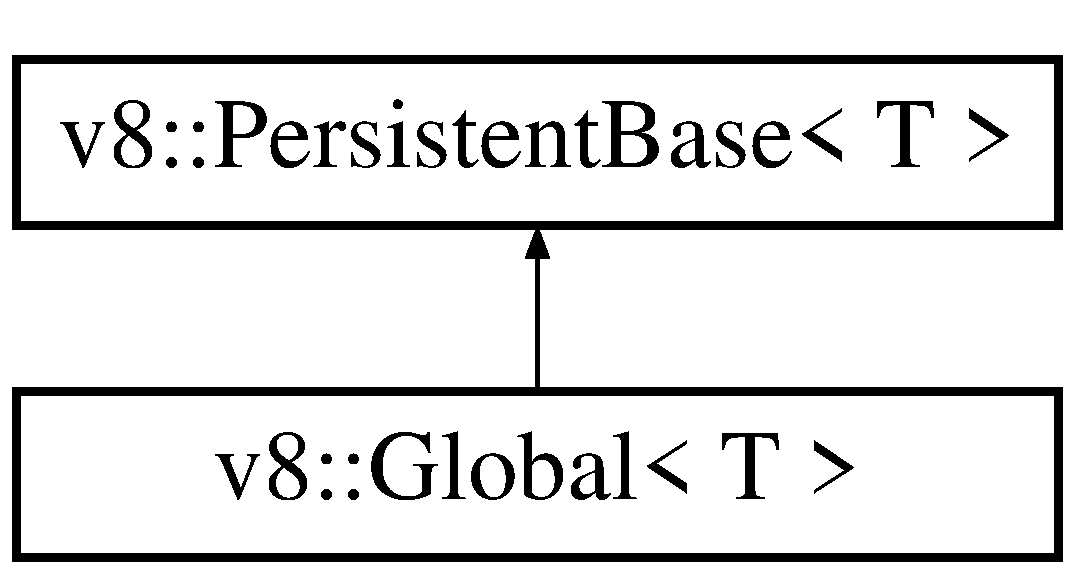
\includegraphics[height=2.000000cm]{classv8_1_1_global}
\end{center}
\end{figure}
\subsection*{Public Types}
\begin{DoxyCompactItemize}
\item 
typedef void {\bfseries Move\+Only\+Type\+For\+C\+P\+P03}\hypertarget{classv8_1_1_global_a295826e79781fe585904e652884db72f}{}\label{classv8_1_1_global_a295826e79781fe585904e652884db72f}

\end{DoxyCompactItemize}
\subsection*{Public Member Functions}
\begin{DoxyCompactItemize}
\item 
V8\+\_\+\+I\+N\+L\+I\+NE \hyperlink{classv8_1_1_global_ab1efdf25ff6305e67f3266a6fe90527e}{Global} ()
\item 
{\footnotesize template$<$class S $>$ }\\V8\+\_\+\+I\+N\+L\+I\+NE \hyperlink{classv8_1_1_global_a8434bb6729eb4cd0cd85ad81bd8344ad}{Global} (\hyperlink{classv8_1_1_isolate}{Isolate} $\ast$isolate, \hyperlink{classv8_1_1_local}{Local}$<$ S $>$ that)
\item 
{\footnotesize template$<$class S $>$ }\\V8\+\_\+\+I\+N\+L\+I\+NE \hyperlink{classv8_1_1_global_a6243ecb28bb97d066065796fa28f7415}{Global} (\hyperlink{classv8_1_1_isolate}{Isolate} $\ast$isolate, const \hyperlink{classv8_1_1_persistent_base}{Persistent\+Base}$<$ S $>$ \&that)
\item 
V8\+\_\+\+I\+N\+L\+I\+NE \hyperlink{classv8_1_1_global_ab8f3c754a58146e6db67012cd74a49cb}{Global} (\hyperlink{classv8_1_1_global}{Global} \&\&other)
\item 
{\footnotesize template$<$class S $>$ }\\V8\+\_\+\+I\+N\+L\+I\+NE \hyperlink{classv8_1_1_global}{Global} \& \hyperlink{classv8_1_1_global_a9d3d7d8f10ad23e413f2027cc15ab209}{operator=} (\hyperlink{classv8_1_1_global}{Global}$<$ S $>$ \&\&rhs)
\item 
\hyperlink{classv8_1_1_global}{Global} \hyperlink{classv8_1_1_global_a914903149cc752468d4a3a11b6089c7e}{Pass} ()
\end{DoxyCompactItemize}
\subsection*{Private Member Functions}
\begin{DoxyCompactItemize}
\item 
{\bfseries Global} (const \hyperlink{classv8_1_1_global}{Global} \&)=delete\hypertarget{classv8_1_1_global_aefdf6b7bc98d7d011e1381b7cac7fa33}{}\label{classv8_1_1_global_aefdf6b7bc98d7d011e1381b7cac7fa33}

\item 
void {\bfseries operator=} (const \hyperlink{classv8_1_1_global}{Global} \&)=delete\hypertarget{classv8_1_1_global_a732256fcf3edd799c55ba559921dff03}{}\label{classv8_1_1_global_a732256fcf3edd799c55ba559921dff03}

\item 
V8\+\_\+\+I\+N\+L\+I\+NE T $\ast$ {\bfseries operator$\ast$} () const \hypertarget{classv8_1_1_global_ade0e3b9e1084a787fff762e31794e129}{}\label{classv8_1_1_global_ade0e3b9e1084a787fff762e31794e129}

\end{DoxyCompactItemize}
\subsection*{Friends}
\begin{DoxyCompactItemize}
\item 
{\footnotesize template$<$class F $>$ }\\class {\bfseries Return\+Value}\hypertarget{classv8_1_1_global_a53f604d3d6f2dc0647df33c9979f116a}{}\label{classv8_1_1_global_a53f604d3d6f2dc0647df33c9979f116a}

\end{DoxyCompactItemize}


\subsection{Detailed Description}
\subsubsection*{template$<$class T$>$\\*
class v8\+::\+Global$<$ T $>$}

A \hyperlink{classv8_1_1_persistent_base}{Persistent\+Base} which has move semantics.

Note\+: \hyperlink{classv8_1_1_persistent}{Persistent} class hierarchy is subject to future changes. 

\subsection{Constructor \& Destructor Documentation}
\index{v8\+::\+Global@{v8\+::\+Global}!Global@{Global}}
\index{Global@{Global}!v8\+::\+Global@{v8\+::\+Global}}
\subsubsection[{\texorpdfstring{Global()}{Global()}}]{\setlength{\rightskip}{0pt plus 5cm}template$<$class T$>$ V8\+\_\+\+I\+N\+L\+I\+NE {\bf v8\+::\+Global}$<$ T $>$\+::{\bf Global} (
\begin{DoxyParamCaption}
{}
\end{DoxyParamCaption}
)\hspace{0.3cm}{\ttfamily [inline]}}\hypertarget{classv8_1_1_global_ab1efdf25ff6305e67f3266a6fe90527e}{}\label{classv8_1_1_global_ab1efdf25ff6305e67f3266a6fe90527e}
A \hyperlink{classv8_1_1_global}{Global} with no storage cell. \index{v8\+::\+Global@{v8\+::\+Global}!Global@{Global}}
\index{Global@{Global}!v8\+::\+Global@{v8\+::\+Global}}
\subsubsection[{\texorpdfstring{Global(\+Isolate $\ast$isolate, Local$<$ S $>$ that)}{Global(Isolate *isolate, Local< S > that)}}]{\setlength{\rightskip}{0pt plus 5cm}template$<$class T$>$ template$<$class S $>$ V8\+\_\+\+I\+N\+L\+I\+NE {\bf v8\+::\+Global}$<$ T $>$\+::{\bf Global} (
\begin{DoxyParamCaption}
\item[{{\bf Isolate} $\ast$}]{isolate, }
\item[{{\bf Local}$<$ S $>$}]{that}
\end{DoxyParamCaption}
)\hspace{0.3cm}{\ttfamily [inline]}}\hypertarget{classv8_1_1_global_a8434bb6729eb4cd0cd85ad81bd8344ad}{}\label{classv8_1_1_global_a8434bb6729eb4cd0cd85ad81bd8344ad}
Construct a \hyperlink{classv8_1_1_global}{Global} from a \hyperlink{classv8_1_1_local}{Local}. When the \hyperlink{classv8_1_1_local}{Local} is non-\/empty, a new storage cell is created pointing to the same object, and no flags are set. \index{v8\+::\+Global@{v8\+::\+Global}!Global@{Global}}
\index{Global@{Global}!v8\+::\+Global@{v8\+::\+Global}}
\subsubsection[{\texorpdfstring{Global(\+Isolate $\ast$isolate, const Persistent\+Base$<$ S $>$ \&that)}{Global(Isolate *isolate, const PersistentBase< S > &that)}}]{\setlength{\rightskip}{0pt plus 5cm}template$<$class T$>$ template$<$class S $>$ V8\+\_\+\+I\+N\+L\+I\+NE {\bf v8\+::\+Global}$<$ T $>$\+::{\bf Global} (
\begin{DoxyParamCaption}
\item[{{\bf Isolate} $\ast$}]{isolate, }
\item[{const {\bf Persistent\+Base}$<$ S $>$ \&}]{that}
\end{DoxyParamCaption}
)\hspace{0.3cm}{\ttfamily [inline]}}\hypertarget{classv8_1_1_global_a6243ecb28bb97d066065796fa28f7415}{}\label{classv8_1_1_global_a6243ecb28bb97d066065796fa28f7415}
Construct a \hyperlink{classv8_1_1_global}{Global} from a \hyperlink{classv8_1_1_persistent_base}{Persistent\+Base}. When the \hyperlink{classv8_1_1_persistent}{Persistent} is non-\/empty, a new storage cell is created pointing to the same object, and no flags are set. \index{v8\+::\+Global@{v8\+::\+Global}!Global@{Global}}
\index{Global@{Global}!v8\+::\+Global@{v8\+::\+Global}}
\subsubsection[{\texorpdfstring{Global(\+Global \&\&other)}{Global(Global &&other)}}]{\setlength{\rightskip}{0pt plus 5cm}template$<$class T$>$ V8\+\_\+\+I\+N\+L\+I\+NE {\bf v8\+::\+Global}$<$ T $>$\+::{\bf Global} (
\begin{DoxyParamCaption}
\item[{{\bf Global}$<$ T $>$ \&\&}]{other}
\end{DoxyParamCaption}
)\hspace{0.3cm}{\ttfamily [inline]}}\hypertarget{classv8_1_1_global_ab8f3c754a58146e6db67012cd74a49cb}{}\label{classv8_1_1_global_ab8f3c754a58146e6db67012cd74a49cb}
Move constructor. 

\subsection{Member Function Documentation}
\index{v8\+::\+Global@{v8\+::\+Global}!operator=@{operator=}}
\index{operator=@{operator=}!v8\+::\+Global@{v8\+::\+Global}}
\subsubsection[{\texorpdfstring{operator=(\+Global$<$ S $>$ \&\&rhs)}{operator=(Global< S > &&rhs)}}]{\setlength{\rightskip}{0pt plus 5cm}template$<$class T$>$ template$<$class S $>$ V8\+\_\+\+I\+N\+L\+I\+NE {\bf Global}\& {\bf v8\+::\+Global}$<$ T $>$\+::operator= (
\begin{DoxyParamCaption}
\item[{{\bf Global}$<$ S $>$ \&\&}]{rhs}
\end{DoxyParamCaption}
)\hspace{0.3cm}{\ttfamily [inline]}}\hypertarget{classv8_1_1_global_a9d3d7d8f10ad23e413f2027cc15ab209}{}\label{classv8_1_1_global_a9d3d7d8f10ad23e413f2027cc15ab209}
Move via assignment. \index{v8\+::\+Global@{v8\+::\+Global}!Pass@{Pass}}
\index{Pass@{Pass}!v8\+::\+Global@{v8\+::\+Global}}
\subsubsection[{\texorpdfstring{Pass()}{Pass()}}]{\setlength{\rightskip}{0pt plus 5cm}template$<$class T$>$ {\bf Global} {\bf v8\+::\+Global}$<$ T $>$\+::Pass (
\begin{DoxyParamCaption}
{}
\end{DoxyParamCaption}
)\hspace{0.3cm}{\ttfamily [inline]}}\hypertarget{classv8_1_1_global_a914903149cc752468d4a3a11b6089c7e}{}\label{classv8_1_1_global_a914903149cc752468d4a3a11b6089c7e}
Pass allows returning uniques from functions, etc. 

The documentation for this class was generated from the following file\+:\begin{DoxyCompactItemize}
\item 
/\+Users/joshgav/node/v8/include/v8.\+h\end{DoxyCompactItemize}

\hypertarget{classv8_1_1_global_value_map}{}\section{v8\+:\+:Global\+Value\+Map$<$ K, V, Traits $>$ Class Template Reference}
\label{classv8_1_1_global_value_map}\index{v8\+::\+Global\+Value\+Map$<$ K, V, Traits $>$@{v8\+::\+Global\+Value\+Map$<$ K, V, Traits $>$}}
Inheritance diagram for v8\+:\+:Global\+Value\+Map$<$ K, V, Traits $>$\+:\begin{figure}[H]
\begin{center}
\leavevmode
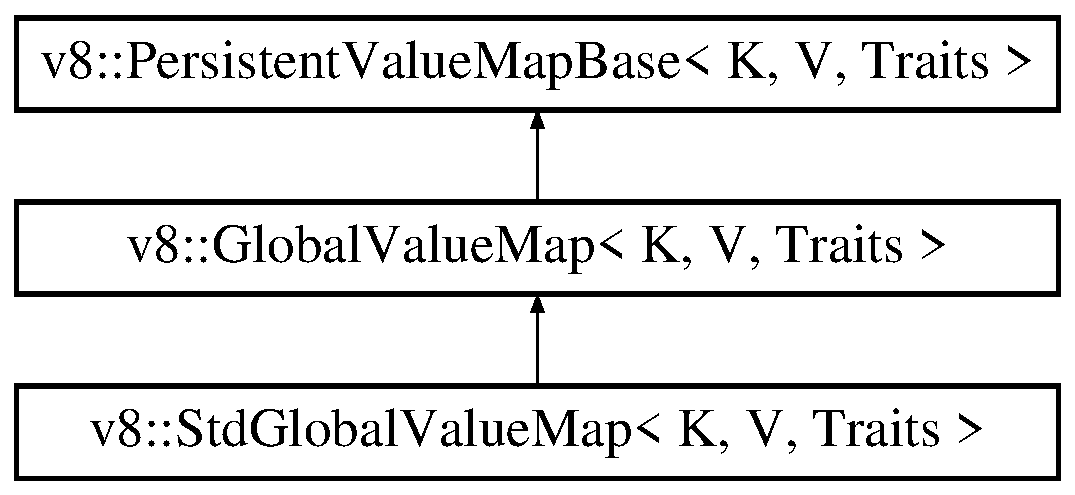
\includegraphics[height=3.000000cm]{classv8_1_1_global_value_map}
\end{center}
\end{figure}
\subsection*{Public Types}
\begin{DoxyCompactItemize}
\item 
typedef \hyperlink{classv8_1_1_persistent_value_map_base}{Persistent\+Value\+Map\+Base}$<$ K, V, Traits $>$\+::\hyperlink{classv8_1_1_persistent_value_map_base_1_1_persistent_value_reference}{Persistent\+Value\+Reference} {\bfseries Persistent\+Value\+Reference}\hypertarget{classv8_1_1_global_value_map_ac01835ce1863e1c577882e31b60efc35}{}\label{classv8_1_1_global_value_map_ac01835ce1863e1c577882e31b60efc35}

\end{DoxyCompactItemize}
\subsection*{Public Member Functions}
\begin{DoxyCompactItemize}
\item 
{\bfseries Global\+Value\+Map} (\hyperlink{classv8_1_1_isolate}{Isolate} $\ast$isolate)\hypertarget{classv8_1_1_global_value_map_a60018c72fdae03d51b687d2a941140f4}{}\label{classv8_1_1_global_value_map_a60018c72fdae03d51b687d2a941140f4}

\item 
\hyperlink{classv8_1_1_global}{Global}$<$ V $>$ \hyperlink{classv8_1_1_global_value_map_aa13f7914642c705b8e96824747ea115a}{Set} (const K \&key, \hyperlink{classv8_1_1_local}{Local}$<$ V $>$ value)
\item 
\hyperlink{classv8_1_1_global}{Global}$<$ V $>$ \hyperlink{classv8_1_1_global_value_map_ac2b02a0105393e6e3ab7e0aeeed9a294}{Set} (const K \&key, \hyperlink{classv8_1_1_global}{Global}$<$ V $>$ value)
\item 
\hyperlink{classv8_1_1_global}{Global}$<$ V $>$ \hyperlink{classv8_1_1_global_value_map_aad73de3912571a2f245454d3edea4a41}{Set\+Unique} (const K \&key, \hyperlink{classv8_1_1_global}{Global}$<$ V $>$ $\ast$persistent)
\item 
\hyperlink{classv8_1_1_global}{Global}$<$ V $>$ \hyperlink{classv8_1_1_global_value_map_aaa5fa26f751c8608716ad5578cd6c1d0}{Set} (const K \&key, \hyperlink{classv8_1_1_global}{Global}$<$ V $>$ value, \hyperlink{classv8_1_1_persistent_value_map_base_1_1_persistent_value_reference}{Persistent\+Value\+Reference} $\ast$reference)
\end{DoxyCompactItemize}
\subsection*{Static Private Member Functions}
\begin{DoxyCompactItemize}
\item 
static void {\bfseries On\+Weak\+Callback} (const \hyperlink{classv8_1_1_weak_callback_info}{Weak\+Callback\+Info}$<$ typename Traits\+::\+Weak\+Callback\+Data\+Type $>$ \&data)\hypertarget{classv8_1_1_global_value_map_af56bf560957d616f34543a2e9d14ca60}{}\label{classv8_1_1_global_value_map_af56bf560957d616f34543a2e9d14ca60}

\item 
static void {\bfseries Second\+Weak\+Callback} (const \hyperlink{classv8_1_1_weak_callback_info}{Weak\+Callback\+Info}$<$ typename Traits\+::\+Weak\+Callback\+Data\+Type $>$ \&data)\hypertarget{classv8_1_1_global_value_map_ae01469ad24dd4bd95c02ee0eac68542f}{}\label{classv8_1_1_global_value_map_ae01469ad24dd4bd95c02ee0eac68542f}

\end{DoxyCompactItemize}
\subsection*{Additional Inherited Members}


\subsection{Member Function Documentation}
\index{v8\+::\+Global\+Value\+Map@{v8\+::\+Global\+Value\+Map}!Set@{Set}}
\index{Set@{Set}!v8\+::\+Global\+Value\+Map@{v8\+::\+Global\+Value\+Map}}
\subsubsection[{\texorpdfstring{Set(const K \&key, Local$<$ V $>$ value)}{Set(const K &key, Local< V > value)}}]{\setlength{\rightskip}{0pt plus 5cm}template$<$typename K , typename V , typename Traits $>$ {\bf Global}$<$V$>$ {\bf v8\+::\+Global\+Value\+Map}$<$ K, V, Traits $>$\+::{\bf Set} (
\begin{DoxyParamCaption}
\item[{const K \&}]{key, }
\item[{{\bf Local}$<$ V $>$}]{value}
\end{DoxyParamCaption}
)\hspace{0.3cm}{\ttfamily [inline]}}\hypertarget{classv8_1_1_global_value_map_aa13f7914642c705b8e96824747ea115a}{}\label{classv8_1_1_global_value_map_aa13f7914642c705b8e96824747ea115a}
Put value into map. Depending on Traits\+::k\+Is\+Weak, the value will be held by the map strongly or weakly. Returns old value as \hyperlink{classv8_1_1_global}{Global}. \index{v8\+::\+Global\+Value\+Map@{v8\+::\+Global\+Value\+Map}!Set@{Set}}
\index{Set@{Set}!v8\+::\+Global\+Value\+Map@{v8\+::\+Global\+Value\+Map}}
\subsubsection[{\texorpdfstring{Set(const K \&key, Global$<$ V $>$ value)}{Set(const K &key, Global< V > value)}}]{\setlength{\rightskip}{0pt plus 5cm}template$<$typename K , typename V , typename Traits $>$ {\bf Global}$<$V$>$ {\bf v8\+::\+Global\+Value\+Map}$<$ K, V, Traits $>$\+::{\bf Set} (
\begin{DoxyParamCaption}
\item[{const K \&}]{key, }
\item[{{\bf Global}$<$ V $>$}]{value}
\end{DoxyParamCaption}
)\hspace{0.3cm}{\ttfamily [inline]}}\hypertarget{classv8_1_1_global_value_map_ac2b02a0105393e6e3ab7e0aeeed9a294}{}\label{classv8_1_1_global_value_map_ac2b02a0105393e6e3ab7e0aeeed9a294}
Put value into map, like \hyperlink{classv8_1_1_global_value_map_aa13f7914642c705b8e96824747ea115a}{Set(const K\&, Local$<$\+V$>$)}. \index{v8\+::\+Global\+Value\+Map@{v8\+::\+Global\+Value\+Map}!Set@{Set}}
\index{Set@{Set}!v8\+::\+Global\+Value\+Map@{v8\+::\+Global\+Value\+Map}}
\subsubsection[{\texorpdfstring{Set(const K \&key, Global$<$ V $>$ value, Persistent\+Value\+Reference $\ast$reference)}{Set(const K &key, Global< V > value, PersistentValueReference *reference)}}]{\setlength{\rightskip}{0pt plus 5cm}template$<$typename K , typename V , typename Traits $>$ {\bf Global}$<$V$>$ {\bf v8\+::\+Global\+Value\+Map}$<$ K, V, Traits $>$\+::{\bf Set} (
\begin{DoxyParamCaption}
\item[{const K \&}]{key, }
\item[{{\bf Global}$<$ V $>$}]{value, }
\item[{{\bf Persistent\+Value\+Reference} $\ast$}]{reference}
\end{DoxyParamCaption}
)\hspace{0.3cm}{\ttfamily [inline]}}\hypertarget{classv8_1_1_global_value_map_aaa5fa26f751c8608716ad5578cd6c1d0}{}\label{classv8_1_1_global_value_map_aaa5fa26f751c8608716ad5578cd6c1d0}
Put a value into the map and update the reference. Restrictions of Get\+Reference apply here as well. \index{v8\+::\+Global\+Value\+Map@{v8\+::\+Global\+Value\+Map}!Set\+Unique@{Set\+Unique}}
\index{Set\+Unique@{Set\+Unique}!v8\+::\+Global\+Value\+Map@{v8\+::\+Global\+Value\+Map}}
\subsubsection[{\texorpdfstring{Set\+Unique(const K \&key, Global$<$ V $>$ $\ast$persistent)}{SetUnique(const K &key, Global< V > *persistent)}}]{\setlength{\rightskip}{0pt plus 5cm}template$<$typename K , typename V , typename Traits $>$ {\bf Global}$<$V$>$ {\bf v8\+::\+Global\+Value\+Map}$<$ K, V, Traits $>$\+::Set\+Unique (
\begin{DoxyParamCaption}
\item[{const K \&}]{key, }
\item[{{\bf Global}$<$ V $>$ $\ast$}]{persistent}
\end{DoxyParamCaption}
)\hspace{0.3cm}{\ttfamily [inline]}}\hypertarget{classv8_1_1_global_value_map_aad73de3912571a2f245454d3edea4a41}{}\label{classv8_1_1_global_value_map_aad73de3912571a2f245454d3edea4a41}
Put the value into the map, and set the \textquotesingle{}weak\textquotesingle{} callback when demanded by the Traits class. 

The documentation for this class was generated from the following file\+:\begin{DoxyCompactItemize}
\item 
include/v8-\/util.\+h\end{DoxyCompactItemize}

\hypertarget{classv8_1_1_handle_scope}{}\section{v8\+:\+:Handle\+Scope Class Reference}
\label{classv8_1_1_handle_scope}\index{v8\+::\+Handle\+Scope@{v8\+::\+Handle\+Scope}}


{\ttfamily \#include $<$v8.\+h$>$}

Inheritance diagram for v8\+:\+:Handle\+Scope\+:\begin{figure}[H]
\begin{center}
\leavevmode
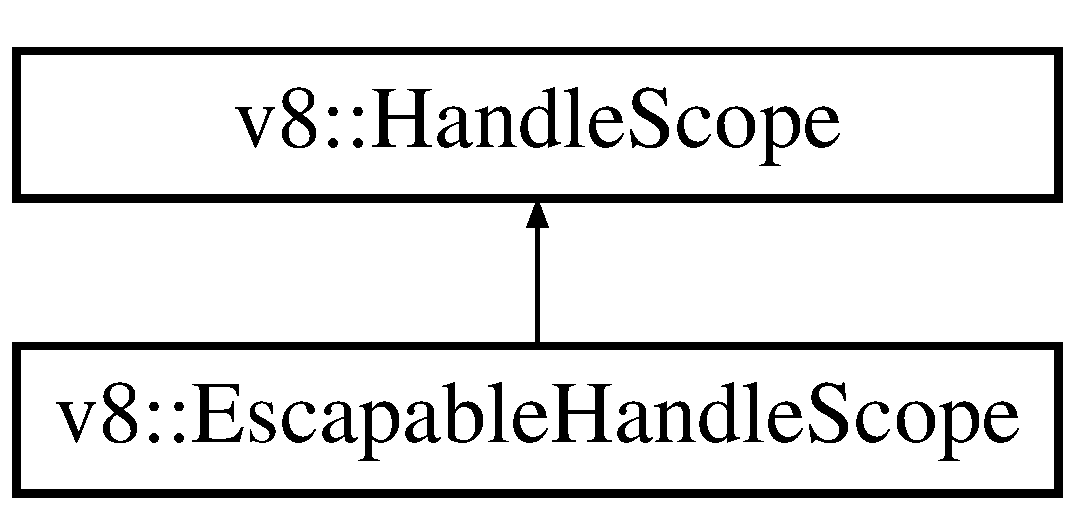
\includegraphics[height=2.000000cm]{classv8_1_1_handle_scope}
\end{center}
\end{figure}
\subsection*{Public Member Functions}
\begin{DoxyCompactItemize}
\item 
{\bfseries Handle\+Scope} (\hyperlink{classv8_1_1_isolate}{Isolate} $\ast$isolate)\hypertarget{classv8_1_1_handle_scope_afdb3053d852ea467f026b025ed431e79}{}\label{classv8_1_1_handle_scope_afdb3053d852ea467f026b025ed431e79}

\item 
V8\+\_\+\+I\+N\+L\+I\+NE \hyperlink{classv8_1_1_isolate}{Isolate} $\ast$ {\bfseries Get\+Isolate} () const \hypertarget{classv8_1_1_handle_scope_a15d1a1e76d8cd8a10d3947c3ca2e8a8d}{}\label{classv8_1_1_handle_scope_a15d1a1e76d8cd8a10d3947c3ca2e8a8d}

\end{DoxyCompactItemize}
\subsection*{Static Public Member Functions}
\begin{DoxyCompactItemize}
\item 
static int \hyperlink{classv8_1_1_handle_scope_abab7214c9b9388b02f575fd5270b7e2f}{Number\+Of\+Handles} (\hyperlink{classv8_1_1_isolate}{Isolate} $\ast$isolate)
\end{DoxyCompactItemize}
\subsection*{Protected Member Functions}
\begin{DoxyCompactItemize}
\item 
void {\bfseries Initialize} (\hyperlink{classv8_1_1_isolate}{Isolate} $\ast$isolate)\hypertarget{classv8_1_1_handle_scope_a7bb8631c1c8756b05e9232b8414dd992}{}\label{classv8_1_1_handle_scope_a7bb8631c1c8756b05e9232b8414dd992}

\end{DoxyCompactItemize}
\subsection*{Static Protected Member Functions}
\begin{DoxyCompactItemize}
\item 
static internal\+::\+Object $\ast$$\ast$ {\bfseries Create\+Handle} (internal\+::\+Isolate $\ast$isolate, internal\+::\+Object $\ast$value)\hypertarget{classv8_1_1_handle_scope_a3f63aa8552a0371606305f58187d80e2}{}\label{classv8_1_1_handle_scope_a3f63aa8552a0371606305f58187d80e2}

\end{DoxyCompactItemize}
\subsection*{Private Member Functions}
\begin{DoxyCompactItemize}
\item 
{\bfseries Handle\+Scope} (const \hyperlink{classv8_1_1_handle_scope}{Handle\+Scope} \&)\hypertarget{classv8_1_1_handle_scope_a7c62e10404e105ec74b86b5d7d5e04fe}{}\label{classv8_1_1_handle_scope_a7c62e10404e105ec74b86b5d7d5e04fe}

\item 
void {\bfseries operator=} (const \hyperlink{classv8_1_1_handle_scope}{Handle\+Scope} \&)\hypertarget{classv8_1_1_handle_scope_a1529e8892e4ec96a845f6dea18f2c2ec}{}\label{classv8_1_1_handle_scope_a1529e8892e4ec96a845f6dea18f2c2ec}

\item 
void $\ast$ {\bfseries operator new} (size\+\_\+t size)\hypertarget{classv8_1_1_handle_scope_a1dd92d6bbc0bf64a66f968e08dad00a2}{}\label{classv8_1_1_handle_scope_a1dd92d6bbc0bf64a66f968e08dad00a2}

\item 
void {\bfseries operator delete} (void $\ast$, size\+\_\+t)\hypertarget{classv8_1_1_handle_scope_ab8ba9daf1a4af951e258c1d4a0f7257c}{}\label{classv8_1_1_handle_scope_ab8ba9daf1a4af951e258c1d4a0f7257c}

\end{DoxyCompactItemize}
\subsection*{Static Private Member Functions}
\begin{DoxyCompactItemize}
\item 
static internal\+::\+Object $\ast$$\ast$ {\bfseries Create\+Handle} (internal\+::\+Heap\+Object $\ast$heap\+\_\+object, internal\+::\+Object $\ast$value)\hypertarget{classv8_1_1_handle_scope_ae8423afe03e4686992deebe9a9b8e7df}{}\label{classv8_1_1_handle_scope_ae8423afe03e4686992deebe9a9b8e7df}

\end{DoxyCompactItemize}
\subsection*{Private Attributes}
\begin{DoxyCompactItemize}
\item 
internal\+::\+Isolate $\ast$ {\bfseries isolate\+\_\+}\hypertarget{classv8_1_1_handle_scope_a57195a6d30243f34c50b4293003cd242}{}\label{classv8_1_1_handle_scope_a57195a6d30243f34c50b4293003cd242}

\item 
internal\+::\+Object $\ast$$\ast$ {\bfseries prev\+\_\+next\+\_\+}\hypertarget{classv8_1_1_handle_scope_a739728a1286a7d92aaeb941db593fa1d}{}\label{classv8_1_1_handle_scope_a739728a1286a7d92aaeb941db593fa1d}

\item 
internal\+::\+Object $\ast$$\ast$ {\bfseries prev\+\_\+limit\+\_\+}\hypertarget{classv8_1_1_handle_scope_a8c56251528a986904e67f28b36900bd9}{}\label{classv8_1_1_handle_scope_a8c56251528a986904e67f28b36900bd9}

\end{DoxyCompactItemize}
\subsection*{Friends}
\begin{DoxyCompactItemize}
\item 
{\footnotesize template$<$class F $>$ }\\class {\bfseries Local}\hypertarget{classv8_1_1_handle_scope_afb872edb4aac7ba55f0da004113aa2b0}{}\label{classv8_1_1_handle_scope_afb872edb4aac7ba55f0da004113aa2b0}

\item 
class {\bfseries Object}\hypertarget{classv8_1_1_handle_scope_a0720b5f434e636e22a3ed34f847eec57}{}\label{classv8_1_1_handle_scope_a0720b5f434e636e22a3ed34f847eec57}

\item 
class {\bfseries Context}\hypertarget{classv8_1_1_handle_scope_ac26c806e60ca4a0547680edb68f6e39b}{}\label{classv8_1_1_handle_scope_ac26c806e60ca4a0547680edb68f6e39b}

\end{DoxyCompactItemize}


\subsection{Detailed Description}
A stack-\/allocated class that governs a number of local handles. After a handle scope has been created, all local handles will be allocated within that handle scope until either the handle scope is deleted or another handle scope is created. If there is already a handle scope and a new one is created, all allocations will take place in the new handle scope until it is deleted. After that, new handles will again be allocated in the original handle scope.

After the handle scope of a local handle has been deleted the garbage collector will no longer track the object stored in the handle and may deallocate it. The behavior of accessing a handle for which the handle scope has been deleted is undefined. 

\subsection{Member Function Documentation}
\index{v8\+::\+Handle\+Scope@{v8\+::\+Handle\+Scope}!Number\+Of\+Handles@{Number\+Of\+Handles}}
\index{Number\+Of\+Handles@{Number\+Of\+Handles}!v8\+::\+Handle\+Scope@{v8\+::\+Handle\+Scope}}
\subsubsection[{\texorpdfstring{Number\+Of\+Handles(\+Isolate $\ast$isolate)}{NumberOfHandles(Isolate *isolate)}}]{\setlength{\rightskip}{0pt plus 5cm}static int v8\+::\+Handle\+Scope\+::\+Number\+Of\+Handles (
\begin{DoxyParamCaption}
\item[{{\bf Isolate} $\ast$}]{isolate}
\end{DoxyParamCaption}
)\hspace{0.3cm}{\ttfamily [static]}}\hypertarget{classv8_1_1_handle_scope_abab7214c9b9388b02f575fd5270b7e2f}{}\label{classv8_1_1_handle_scope_abab7214c9b9388b02f575fd5270b7e2f}
Counts the number of allocated handles. 

The documentation for this class was generated from the following file\+:\begin{DoxyCompactItemize}
\item 
/\+Users/joshgav/node/v8/include/v8.\+h\end{DoxyCompactItemize}

\hypertarget{classv8_1_1_heap_graph_edge}{}\section{v8\+:\+:Heap\+Graph\+Edge Class Reference}
\label{classv8_1_1_heap_graph_edge}\index{v8\+::\+Heap\+Graph\+Edge@{v8\+::\+Heap\+Graph\+Edge}}


{\ttfamily \#include $<$v8-\/profiler.\+h$>$}

\subsection*{Public Types}
\begin{DoxyCompactItemize}
\item 
enum {\bfseries Type} \{ \\*
{\bfseries k\+Context\+Variable} = 0, 
\\*
{\bfseries k\+Element} = 1, 
\\*
{\bfseries k\+Property} = 2, 
\\*
{\bfseries k\+Internal} = 3, 
\\*
{\bfseries k\+Hidden} = 4, 
\\*
{\bfseries k\+Shortcut} = 5, 
\\*
{\bfseries k\+Weak} = 6
 \}\hypertarget{classv8_1_1_heap_graph_edge_a252500cf4307fe9e4fcb0335a907259b}{}\label{classv8_1_1_heap_graph_edge_a252500cf4307fe9e4fcb0335a907259b}

\end{DoxyCompactItemize}
\subsection*{Public Member Functions}
\begin{DoxyCompactItemize}
\item 
Type \hyperlink{classv8_1_1_heap_graph_edge_a7f4923098074ee4c47d901f363728d08}{Get\+Type} () const 
\item 
\hyperlink{classv8_1_1_local}{Local}$<$ \hyperlink{classv8_1_1_value}{Value} $>$ \hyperlink{classv8_1_1_heap_graph_edge_a295702dc31ef38dadb54143f2a76e12e}{Get\+Name} () const 
\item 
const \hyperlink{classv8_1_1_heap_graph_node}{Heap\+Graph\+Node} $\ast$ \hyperlink{classv8_1_1_heap_graph_edge_acd43a5082f1862b7c0c0094fc75af631}{Get\+From\+Node} () const 
\item 
const \hyperlink{classv8_1_1_heap_graph_node}{Heap\+Graph\+Node} $\ast$ \hyperlink{classv8_1_1_heap_graph_edge_ad8fd8fa121a0e778a8b120a0c5fa227c}{Get\+To\+Node} () const 
\end{DoxyCompactItemize}


\subsection{Detailed Description}
Heap\+Snapshot\+Edge represents a directed connection between heap graph nodes\+: from retainers to retained nodes. 

\subsection{Member Function Documentation}
\index{v8\+::\+Heap\+Graph\+Edge@{v8\+::\+Heap\+Graph\+Edge}!Get\+From\+Node@{Get\+From\+Node}}
\index{Get\+From\+Node@{Get\+From\+Node}!v8\+::\+Heap\+Graph\+Edge@{v8\+::\+Heap\+Graph\+Edge}}
\subsubsection[{\texorpdfstring{Get\+From\+Node() const }{GetFromNode() const }}]{\setlength{\rightskip}{0pt plus 5cm}const {\bf Heap\+Graph\+Node}$\ast$ v8\+::\+Heap\+Graph\+Edge\+::\+Get\+From\+Node (
\begin{DoxyParamCaption}
{}
\end{DoxyParamCaption}
) const}\hypertarget{classv8_1_1_heap_graph_edge_acd43a5082f1862b7c0c0094fc75af631}{}\label{classv8_1_1_heap_graph_edge_acd43a5082f1862b7c0c0094fc75af631}
Returns origin node. \index{v8\+::\+Heap\+Graph\+Edge@{v8\+::\+Heap\+Graph\+Edge}!Get\+Name@{Get\+Name}}
\index{Get\+Name@{Get\+Name}!v8\+::\+Heap\+Graph\+Edge@{v8\+::\+Heap\+Graph\+Edge}}
\subsubsection[{\texorpdfstring{Get\+Name() const }{GetName() const }}]{\setlength{\rightskip}{0pt plus 5cm}{\bf Local}$<${\bf Value}$>$ v8\+::\+Heap\+Graph\+Edge\+::\+Get\+Name (
\begin{DoxyParamCaption}
{}
\end{DoxyParamCaption}
) const}\hypertarget{classv8_1_1_heap_graph_edge_a295702dc31ef38dadb54143f2a76e12e}{}\label{classv8_1_1_heap_graph_edge_a295702dc31ef38dadb54143f2a76e12e}
Returns edge name. This can be a variable name, an element index, or a property name. \index{v8\+::\+Heap\+Graph\+Edge@{v8\+::\+Heap\+Graph\+Edge}!Get\+To\+Node@{Get\+To\+Node}}
\index{Get\+To\+Node@{Get\+To\+Node}!v8\+::\+Heap\+Graph\+Edge@{v8\+::\+Heap\+Graph\+Edge}}
\subsubsection[{\texorpdfstring{Get\+To\+Node() const }{GetToNode() const }}]{\setlength{\rightskip}{0pt plus 5cm}const {\bf Heap\+Graph\+Node}$\ast$ v8\+::\+Heap\+Graph\+Edge\+::\+Get\+To\+Node (
\begin{DoxyParamCaption}
{}
\end{DoxyParamCaption}
) const}\hypertarget{classv8_1_1_heap_graph_edge_ad8fd8fa121a0e778a8b120a0c5fa227c}{}\label{classv8_1_1_heap_graph_edge_ad8fd8fa121a0e778a8b120a0c5fa227c}
Returns destination node. \index{v8\+::\+Heap\+Graph\+Edge@{v8\+::\+Heap\+Graph\+Edge}!Get\+Type@{Get\+Type}}
\index{Get\+Type@{Get\+Type}!v8\+::\+Heap\+Graph\+Edge@{v8\+::\+Heap\+Graph\+Edge}}
\subsubsection[{\texorpdfstring{Get\+Type() const }{GetType() const }}]{\setlength{\rightskip}{0pt plus 5cm}Type v8\+::\+Heap\+Graph\+Edge\+::\+Get\+Type (
\begin{DoxyParamCaption}
{}
\end{DoxyParamCaption}
) const}\hypertarget{classv8_1_1_heap_graph_edge_a7f4923098074ee4c47d901f363728d08}{}\label{classv8_1_1_heap_graph_edge_a7f4923098074ee4c47d901f363728d08}
Returns edge type (see Heap\+Graph\+Edge\+::\+Type). 

The documentation for this class was generated from the following file\+:\begin{DoxyCompactItemize}
\item 
include/v8-\/profiler.\+h\end{DoxyCompactItemize}

\hypertarget{classv8_1_1_heap_graph_node}{}\section{v8\+:\+:Heap\+Graph\+Node Class Reference}
\label{classv8_1_1_heap_graph_node}\index{v8\+::\+Heap\+Graph\+Node@{v8\+::\+Heap\+Graph\+Node}}


{\ttfamily \#include $<$v8-\/profiler.\+h$>$}

\subsection*{Public Types}
\begin{DoxyCompactItemize}
\item 
enum {\bfseries Type} \{ \\*
{\bfseries k\+Hidden} = 0, 
\\*
{\bfseries k\+Array} = 1, 
\\*
{\bfseries k\+String} = 2, 
\\*
{\bfseries k\+Object} = 3, 
\\*
{\bfseries k\+Code} = 4, 
\\*
{\bfseries k\+Closure} = 5, 
\\*
{\bfseries k\+Reg\+Exp} = 6, 
\\*
{\bfseries k\+Heap\+Number} = 7, 
\\*
{\bfseries k\+Native} = 8, 
\\*
{\bfseries k\+Synthetic} = 9, 
\\*
{\bfseries k\+Cons\+String} = 10, 
\\*
{\bfseries k\+Sliced\+String} = 11, 
\\*
{\bfseries k\+Symbol} = 12, 
\\*
{\bfseries k\+Simd\+Value} = 13
 \}\hypertarget{classv8_1_1_heap_graph_node_ab674a58103a51abc56f99edc6a1479ed}{}\label{classv8_1_1_heap_graph_node_ab674a58103a51abc56f99edc6a1479ed}

\end{DoxyCompactItemize}
\subsection*{Public Member Functions}
\begin{DoxyCompactItemize}
\item 
Type \hyperlink{classv8_1_1_heap_graph_node_a5e07fc855bded52229e62b855fa08c5d}{Get\+Type} () const 
\item 
\hyperlink{classv8_1_1_local}{Local}$<$ \hyperlink{classv8_1_1_string}{String} $>$ \hyperlink{classv8_1_1_heap_graph_node_afd02d17040ae74f40d60d921795aacdb}{Get\+Name} () const 
\item 
Snapshot\+Object\+Id \hyperlink{classv8_1_1_heap_graph_node_a0faf2a07888af9ca938b3ac089500b4c}{Get\+Id} () const 
\item 
size\+\_\+t \hyperlink{classv8_1_1_heap_graph_node_a5f6f1e87efce0b297c3ffad0b50f34d5}{Get\+Shallow\+Size} () const 
\item 
int \hyperlink{classv8_1_1_heap_graph_node_a0a49abe006755dd5536d15ae42f552d4}{Get\+Children\+Count} () const 
\item 
const \hyperlink{classv8_1_1_heap_graph_edge}{Heap\+Graph\+Edge} $\ast$ \hyperlink{classv8_1_1_heap_graph_node_ac3435611573e58b6614aeaab68442905}{Get\+Child} (int index) const 
\end{DoxyCompactItemize}


\subsection{Detailed Description}
\hyperlink{classv8_1_1_heap_graph_node}{Heap\+Graph\+Node} represents a node in a heap graph. 

\subsection{Member Function Documentation}
\index{v8\+::\+Heap\+Graph\+Node@{v8\+::\+Heap\+Graph\+Node}!Get\+Child@{Get\+Child}}
\index{Get\+Child@{Get\+Child}!v8\+::\+Heap\+Graph\+Node@{v8\+::\+Heap\+Graph\+Node}}
\subsubsection[{\texorpdfstring{Get\+Child(int index) const }{GetChild(int index) const }}]{\setlength{\rightskip}{0pt plus 5cm}const {\bf Heap\+Graph\+Edge}$\ast$ v8\+::\+Heap\+Graph\+Node\+::\+Get\+Child (
\begin{DoxyParamCaption}
\item[{int}]{index}
\end{DoxyParamCaption}
) const}\hypertarget{classv8_1_1_heap_graph_node_ac3435611573e58b6614aeaab68442905}{}\label{classv8_1_1_heap_graph_node_ac3435611573e58b6614aeaab68442905}
Retrieves a child by index. \index{v8\+::\+Heap\+Graph\+Node@{v8\+::\+Heap\+Graph\+Node}!Get\+Children\+Count@{Get\+Children\+Count}}
\index{Get\+Children\+Count@{Get\+Children\+Count}!v8\+::\+Heap\+Graph\+Node@{v8\+::\+Heap\+Graph\+Node}}
\subsubsection[{\texorpdfstring{Get\+Children\+Count() const }{GetChildrenCount() const }}]{\setlength{\rightskip}{0pt plus 5cm}int v8\+::\+Heap\+Graph\+Node\+::\+Get\+Children\+Count (
\begin{DoxyParamCaption}
{}
\end{DoxyParamCaption}
) const}\hypertarget{classv8_1_1_heap_graph_node_a0a49abe006755dd5536d15ae42f552d4}{}\label{classv8_1_1_heap_graph_node_a0a49abe006755dd5536d15ae42f552d4}
Returns child nodes count of the node. \index{v8\+::\+Heap\+Graph\+Node@{v8\+::\+Heap\+Graph\+Node}!Get\+Id@{Get\+Id}}
\index{Get\+Id@{Get\+Id}!v8\+::\+Heap\+Graph\+Node@{v8\+::\+Heap\+Graph\+Node}}
\subsubsection[{\texorpdfstring{Get\+Id() const }{GetId() const }}]{\setlength{\rightskip}{0pt plus 5cm}Snapshot\+Object\+Id v8\+::\+Heap\+Graph\+Node\+::\+Get\+Id (
\begin{DoxyParamCaption}
{}
\end{DoxyParamCaption}
) const}\hypertarget{classv8_1_1_heap_graph_node_a0faf2a07888af9ca938b3ac089500b4c}{}\label{classv8_1_1_heap_graph_node_a0faf2a07888af9ca938b3ac089500b4c}
Returns node id. For the same heap object, the id remains the same across all snapshots. \index{v8\+::\+Heap\+Graph\+Node@{v8\+::\+Heap\+Graph\+Node}!Get\+Name@{Get\+Name}}
\index{Get\+Name@{Get\+Name}!v8\+::\+Heap\+Graph\+Node@{v8\+::\+Heap\+Graph\+Node}}
\subsubsection[{\texorpdfstring{Get\+Name() const }{GetName() const }}]{\setlength{\rightskip}{0pt plus 5cm}{\bf Local}$<${\bf String}$>$ v8\+::\+Heap\+Graph\+Node\+::\+Get\+Name (
\begin{DoxyParamCaption}
{}
\end{DoxyParamCaption}
) const}\hypertarget{classv8_1_1_heap_graph_node_afd02d17040ae74f40d60d921795aacdb}{}\label{classv8_1_1_heap_graph_node_afd02d17040ae74f40d60d921795aacdb}
Returns node name. Depending on node\textquotesingle{}s type this can be the name of the constructor (for objects), the name of the function (for closures), string value, or an empty string (for compiled code). \index{v8\+::\+Heap\+Graph\+Node@{v8\+::\+Heap\+Graph\+Node}!Get\+Shallow\+Size@{Get\+Shallow\+Size}}
\index{Get\+Shallow\+Size@{Get\+Shallow\+Size}!v8\+::\+Heap\+Graph\+Node@{v8\+::\+Heap\+Graph\+Node}}
\subsubsection[{\texorpdfstring{Get\+Shallow\+Size() const }{GetShallowSize() const }}]{\setlength{\rightskip}{0pt plus 5cm}size\+\_\+t v8\+::\+Heap\+Graph\+Node\+::\+Get\+Shallow\+Size (
\begin{DoxyParamCaption}
{}
\end{DoxyParamCaption}
) const}\hypertarget{classv8_1_1_heap_graph_node_a5f6f1e87efce0b297c3ffad0b50f34d5}{}\label{classv8_1_1_heap_graph_node_a5f6f1e87efce0b297c3ffad0b50f34d5}
Returns node\textquotesingle{}s own size, in bytes. \index{v8\+::\+Heap\+Graph\+Node@{v8\+::\+Heap\+Graph\+Node}!Get\+Type@{Get\+Type}}
\index{Get\+Type@{Get\+Type}!v8\+::\+Heap\+Graph\+Node@{v8\+::\+Heap\+Graph\+Node}}
\subsubsection[{\texorpdfstring{Get\+Type() const }{GetType() const }}]{\setlength{\rightskip}{0pt plus 5cm}Type v8\+::\+Heap\+Graph\+Node\+::\+Get\+Type (
\begin{DoxyParamCaption}
{}
\end{DoxyParamCaption}
) const}\hypertarget{classv8_1_1_heap_graph_node_a5e07fc855bded52229e62b855fa08c5d}{}\label{classv8_1_1_heap_graph_node_a5e07fc855bded52229e62b855fa08c5d}
Returns node type (see Heap\+Graph\+Node\+::\+Type). 

The documentation for this class was generated from the following file\+:\begin{DoxyCompactItemize}
\item 
/\+Users/joshgav/node/v8/include/v8-\/profiler.\+h\end{DoxyCompactItemize}

\hypertarget{classv8_1_1_heap_object_statistics}{}\section{v8\+:\+:Heap\+Object\+Statistics Class Reference}
\label{classv8_1_1_heap_object_statistics}\index{v8\+::\+Heap\+Object\+Statistics@{v8\+::\+Heap\+Object\+Statistics}}
\subsection*{Public Member Functions}
\begin{DoxyCompactItemize}
\item 
const char $\ast$ {\bfseries object\+\_\+type} ()\hypertarget{classv8_1_1_heap_object_statistics_a2e9a0e6c13c9db9ff2e7325dddb533b7}{}\label{classv8_1_1_heap_object_statistics_a2e9a0e6c13c9db9ff2e7325dddb533b7}

\item 
const char $\ast$ {\bfseries object\+\_\+sub\+\_\+type} ()\hypertarget{classv8_1_1_heap_object_statistics_a148312ee9ba0ed04bd0c51c0aeb54bc1}{}\label{classv8_1_1_heap_object_statistics_a148312ee9ba0ed04bd0c51c0aeb54bc1}

\item 
size\+\_\+t {\bfseries object\+\_\+count} ()\hypertarget{classv8_1_1_heap_object_statistics_a80ae1b0b1ba566bbb68c98aedb9948ab}{}\label{classv8_1_1_heap_object_statistics_a80ae1b0b1ba566bbb68c98aedb9948ab}

\item 
size\+\_\+t {\bfseries object\+\_\+size} ()\hypertarget{classv8_1_1_heap_object_statistics_a973a50d32c03260eda0699e58f9049ff}{}\label{classv8_1_1_heap_object_statistics_a973a50d32c03260eda0699e58f9049ff}

\end{DoxyCompactItemize}
\subsection*{Private Attributes}
\begin{DoxyCompactItemize}
\item 
const char $\ast$ {\bfseries object\+\_\+type\+\_\+}\hypertarget{classv8_1_1_heap_object_statistics_a990809fcfd32b55d2ad0aa4ec9452004}{}\label{classv8_1_1_heap_object_statistics_a990809fcfd32b55d2ad0aa4ec9452004}

\item 
const char $\ast$ {\bfseries object\+\_\+sub\+\_\+type\+\_\+}\hypertarget{classv8_1_1_heap_object_statistics_aa29ddbbedd1431276623fb6b12ef5945}{}\label{classv8_1_1_heap_object_statistics_aa29ddbbedd1431276623fb6b12ef5945}

\item 
size\+\_\+t {\bfseries object\+\_\+count\+\_\+}\hypertarget{classv8_1_1_heap_object_statistics_a7fc97890029c38eee4408acdc3013520}{}\label{classv8_1_1_heap_object_statistics_a7fc97890029c38eee4408acdc3013520}

\item 
size\+\_\+t {\bfseries object\+\_\+size\+\_\+}\hypertarget{classv8_1_1_heap_object_statistics_afe0db82334e2f2eb0e8d3a7932180534}{}\label{classv8_1_1_heap_object_statistics_afe0db82334e2f2eb0e8d3a7932180534}

\end{DoxyCompactItemize}
\subsection*{Friends}
\begin{DoxyCompactItemize}
\item 
class {\bfseries Isolate}\hypertarget{classv8_1_1_heap_object_statistics_aba4f0964bdacf2bbf62cf876e5d28d0a}{}\label{classv8_1_1_heap_object_statistics_aba4f0964bdacf2bbf62cf876e5d28d0a}

\end{DoxyCompactItemize}


The documentation for this class was generated from the following files\+:\begin{DoxyCompactItemize}
\item 
/\+Users/joshgav/node/v8/include/v8.\+h\item 
/\+Users/joshgav/node/v8/src/api.\+cc\end{DoxyCompactItemize}

\hypertarget{classv8_1_1_heap_profiler}{}\section{v8\+:\+:Heap\+Profiler Class Reference}
\label{classv8_1_1_heap_profiler}\index{v8\+::\+Heap\+Profiler@{v8\+::\+Heap\+Profiler}}


{\ttfamily \#include $<$v8-\/profiler.\+h$>$}

\subsection*{Classes}
\begin{DoxyCompactItemize}
\item 
class \hyperlink{classv8_1_1_heap_profiler_1_1_object_name_resolver}{Object\+Name\+Resolver}
\end{DoxyCompactItemize}
\subsection*{Public Types}
\begin{DoxyCompactItemize}
\item 
enum {\bfseries Sampling\+Flags} \{ \\*
{\bfseries k\+Sampling\+No\+Flags} = 0, 
\\*
{\bfseries k\+Sampling\+Force\+GC} = 1 $<$$<$ 0
 \}\hypertarget{classv8_1_1_heap_profiler_aa7826fbe67065080b08309e8f649e049}{}\label{classv8_1_1_heap_profiler_aa7826fbe67065080b08309e8f649e049}

\item 
typedef \hyperlink{classv8_1_1_retained_object_info}{Retained\+Object\+Info} $\ast$($\ast$ \hyperlink{classv8_1_1_heap_profiler_a677025dd201fd832e0464e5ab0b0d0d4}{Wrapper\+Info\+Callback}) (uint16\+\_\+t class\+\_\+id, \hyperlink{classv8_1_1_local}{Local}$<$ \hyperlink{classv8_1_1_value}{Value} $>$ wrapper)
\end{DoxyCompactItemize}
\subsection*{Public Member Functions}
\begin{DoxyCompactItemize}
\item 
int \hyperlink{classv8_1_1_heap_profiler_a24830775a0ab938eb0a29ed8f3dfd265}{Get\+Snapshot\+Count} ()
\item 
const \hyperlink{classv8_1_1_heap_snapshot}{Heap\+Snapshot} $\ast$ \hyperlink{classv8_1_1_heap_profiler_af9093f6ca6e5558315f354c7ccb55484}{Get\+Heap\+Snapshot} (int index)
\item 
Snapshot\+Object\+Id \hyperlink{classv8_1_1_heap_profiler_ab926a1f1ed95b731d4ef3133e67eef19}{Get\+Object\+Id} (\hyperlink{classv8_1_1_local}{Local}$<$ \hyperlink{classv8_1_1_value}{Value} $>$ value)
\item 
\hyperlink{classv8_1_1_local}{Local}$<$ \hyperlink{classv8_1_1_value}{Value} $>$ \hyperlink{classv8_1_1_heap_profiler_ace729f9b7dbb2ca8b2fd67551bf5aae8}{Find\+Object\+By\+Id} (Snapshot\+Object\+Id id)
\item 
void \hyperlink{classv8_1_1_heap_profiler_a8a90c630543ed1875cbf9166239ff8d3}{Clear\+Object\+Ids} ()
\item 
const \hyperlink{classv8_1_1_heap_snapshot}{Heap\+Snapshot} $\ast$ \hyperlink{classv8_1_1_heap_profiler_a4af9159585ab024175d8eff551804ea8}{Take\+Heap\+Snapshot} (\hyperlink{classv8_1_1_activity_control}{Activity\+Control} $\ast$control=N\+U\+LL, \hyperlink{classv8_1_1_heap_profiler_1_1_object_name_resolver}{Object\+Name\+Resolver} $\ast$global\+\_\+object\+\_\+name\+\_\+resolver=N\+U\+LL)
\item 
void \hyperlink{classv8_1_1_heap_profiler_a02917db133b7efd468c9c73075a15171}{Start\+Tracking\+Heap\+Objects} (bool track\+\_\+allocations=false)
\item 
Snapshot\+Object\+Id \hyperlink{classv8_1_1_heap_profiler_a756d71126e0effc7543fb33e856dd738}{Get\+Heap\+Stats} (\hyperlink{classv8_1_1_output_stream}{Output\+Stream} $\ast$stream, int64\+\_\+t $\ast$timestamp\+\_\+us=N\+U\+LL)
\item 
void \hyperlink{classv8_1_1_heap_profiler_ae448d9474ae34781133d4a4547b08cb1}{Stop\+Tracking\+Heap\+Objects} ()
\item 
bool \hyperlink{classv8_1_1_heap_profiler_a6b9450bbf1f4e1a4909df92d4df4a174}{Start\+Sampling\+Heap\+Profiler} (uint64\+\_\+t sample\+\_\+interval=512 $\ast$1024, int stack\+\_\+depth=16, Sampling\+Flags flags=k\+Sampling\+No\+Flags)
\item 
void \hyperlink{classv8_1_1_heap_profiler_abc43e12e6febb087be251c0629ff17bf}{Stop\+Sampling\+Heap\+Profiler} ()
\item 
\hyperlink{classv8_1_1_allocation_profile}{Allocation\+Profile} $\ast$ \hyperlink{classv8_1_1_heap_profiler_aaadb22168da6a2889796ed3b5638cd50}{Get\+Allocation\+Profile} ()
\item 
void \hyperlink{classv8_1_1_heap_profiler_a6a75bcc6d8350858597b6a6ce5e349a2}{Delete\+All\+Heap\+Snapshots} ()
\item 
void \hyperlink{classv8_1_1_heap_profiler_a7744cf111ad9c6b0b409841f8ed8bcdd}{Set\+Wrapper\+Class\+Info\+Provider} (uint16\+\_\+t class\+\_\+id, \hyperlink{classv8_1_1_heap_profiler_a677025dd201fd832e0464e5ab0b0d0d4}{Wrapper\+Info\+Callback} callback)
\item 
size\+\_\+t \hyperlink{classv8_1_1_heap_profiler_a76435e93466db7519fb31417ea39b13e}{Get\+Profiler\+Memory\+Size} ()
\item 
void \hyperlink{classv8_1_1_heap_profiler_a70821ff8e1c2cc92c310c5c4f1fa5ec7}{Set\+Retained\+Object\+Info} (\hyperlink{classv8_1_1_unique_id}{Unique\+Id} id, \hyperlink{classv8_1_1_retained_object_info}{Retained\+Object\+Info} $\ast$info)
\end{DoxyCompactItemize}
\subsection*{Static Public Attributes}
\begin{DoxyCompactItemize}
\item 
static const Snapshot\+Object\+Id \hyperlink{classv8_1_1_heap_profiler_abf2b9d8facb18473f9b124ab8baf5786}{k\+Unknown\+Object\+Id} = 0
\item 
static const uint16\+\_\+t \hyperlink{classv8_1_1_heap_profiler_a272c9af3ea5cd90a2737af3d22a7eb78}{k\+Persistent\+Handle\+No\+Class\+Id} = 0
\end{DoxyCompactItemize}
\subsection*{Private Member Functions}
\begin{DoxyCompactItemize}
\item 
{\bfseries Heap\+Profiler} (const \hyperlink{classv8_1_1_heap_profiler}{Heap\+Profiler} \&)\hypertarget{classv8_1_1_heap_profiler_abb7dd8b5c784388e6ca2266344f18056}{}\label{classv8_1_1_heap_profiler_abb7dd8b5c784388e6ca2266344f18056}

\item 
\hyperlink{classv8_1_1_heap_profiler}{Heap\+Profiler} \& {\bfseries operator=} (const \hyperlink{classv8_1_1_heap_profiler}{Heap\+Profiler} \&)\hypertarget{classv8_1_1_heap_profiler_a9792e8ddde522f8e2aa97005c0e6bc8f}{}\label{classv8_1_1_heap_profiler_a9792e8ddde522f8e2aa97005c0e6bc8f}

\end{DoxyCompactItemize}


\subsection{Detailed Description}
Interface for controlling heap profiling. Instance of the profiler can be retrieved using \hyperlink{classv8_1_1_isolate_a9c48259615e8370f6f0efd27cd7f99a6}{v8\+::\+Isolate\+::\+Get\+Heap\+Profiler}. 

\subsection{Member Typedef Documentation}
\index{v8\+::\+Heap\+Profiler@{v8\+::\+Heap\+Profiler}!Wrapper\+Info\+Callback@{Wrapper\+Info\+Callback}}
\index{Wrapper\+Info\+Callback@{Wrapper\+Info\+Callback}!v8\+::\+Heap\+Profiler@{v8\+::\+Heap\+Profiler}}
\subsubsection[{\texorpdfstring{Wrapper\+Info\+Callback}{WrapperInfoCallback}}]{\setlength{\rightskip}{0pt plus 5cm}typedef {\bf Retained\+Object\+Info}$\ast$($\ast$ v8\+::\+Heap\+Profiler\+::\+Wrapper\+Info\+Callback) (uint16\+\_\+t class\+\_\+id, {\bf Local}$<$ {\bf Value} $>$ wrapper)}\hypertarget{classv8_1_1_heap_profiler_a677025dd201fd832e0464e5ab0b0d0d4}{}\label{classv8_1_1_heap_profiler_a677025dd201fd832e0464e5ab0b0d0d4}
Callback function invoked for obtaining \hyperlink{classv8_1_1_retained_object_info}{Retained\+Object\+Info} for the given Java\+Script wrapper object. It is prohibited to enter \hyperlink{classv8_1_1_v8}{V8} while the callback is running\+: only getters on the handle and Get\+Pointer\+From\+Internal\+Field on the objects are allowed. 

\subsection{Member Function Documentation}
\index{v8\+::\+Heap\+Profiler@{v8\+::\+Heap\+Profiler}!Clear\+Object\+Ids@{Clear\+Object\+Ids}}
\index{Clear\+Object\+Ids@{Clear\+Object\+Ids}!v8\+::\+Heap\+Profiler@{v8\+::\+Heap\+Profiler}}
\subsubsection[{\texorpdfstring{Clear\+Object\+Ids()}{ClearObjectIds()}}]{\setlength{\rightskip}{0pt plus 5cm}void v8\+::\+Heap\+Profiler\+::\+Clear\+Object\+Ids (
\begin{DoxyParamCaption}
{}
\end{DoxyParamCaption}
)}\hypertarget{classv8_1_1_heap_profiler_a8a90c630543ed1875cbf9166239ff8d3}{}\label{classv8_1_1_heap_profiler_a8a90c630543ed1875cbf9166239ff8d3}
Clears internal map from Snapshot\+Object\+Id to heap object. The new objects will not be added into it unless a heap snapshot is taken or heap object tracking is kicked off. \index{v8\+::\+Heap\+Profiler@{v8\+::\+Heap\+Profiler}!Delete\+All\+Heap\+Snapshots@{Delete\+All\+Heap\+Snapshots}}
\index{Delete\+All\+Heap\+Snapshots@{Delete\+All\+Heap\+Snapshots}!v8\+::\+Heap\+Profiler@{v8\+::\+Heap\+Profiler}}
\subsubsection[{\texorpdfstring{Delete\+All\+Heap\+Snapshots()}{DeleteAllHeapSnapshots()}}]{\setlength{\rightskip}{0pt plus 5cm}void v8\+::\+Heap\+Profiler\+::\+Delete\+All\+Heap\+Snapshots (
\begin{DoxyParamCaption}
{}
\end{DoxyParamCaption}
)}\hypertarget{classv8_1_1_heap_profiler_a6a75bcc6d8350858597b6a6ce5e349a2}{}\label{classv8_1_1_heap_profiler_a6a75bcc6d8350858597b6a6ce5e349a2}
Deletes all snapshots taken. All previously returned pointers to snapshots and their contents become invalid after this call. \index{v8\+::\+Heap\+Profiler@{v8\+::\+Heap\+Profiler}!Find\+Object\+By\+Id@{Find\+Object\+By\+Id}}
\index{Find\+Object\+By\+Id@{Find\+Object\+By\+Id}!v8\+::\+Heap\+Profiler@{v8\+::\+Heap\+Profiler}}
\subsubsection[{\texorpdfstring{Find\+Object\+By\+Id(\+Snapshot\+Object\+Id id)}{FindObjectById(SnapshotObjectId id)}}]{\setlength{\rightskip}{0pt plus 5cm}{\bf Local}$<${\bf Value}$>$ v8\+::\+Heap\+Profiler\+::\+Find\+Object\+By\+Id (
\begin{DoxyParamCaption}
\item[{Snapshot\+Object\+Id}]{id}
\end{DoxyParamCaption}
)}\hypertarget{classv8_1_1_heap_profiler_ace729f9b7dbb2ca8b2fd67551bf5aae8}{}\label{classv8_1_1_heap_profiler_ace729f9b7dbb2ca8b2fd67551bf5aae8}
Returns heap object with given Snapshot\+Object\+Id if the object is alive, otherwise empty handle is returned. \index{v8\+::\+Heap\+Profiler@{v8\+::\+Heap\+Profiler}!Get\+Allocation\+Profile@{Get\+Allocation\+Profile}}
\index{Get\+Allocation\+Profile@{Get\+Allocation\+Profile}!v8\+::\+Heap\+Profiler@{v8\+::\+Heap\+Profiler}}
\subsubsection[{\texorpdfstring{Get\+Allocation\+Profile()}{GetAllocationProfile()}}]{\setlength{\rightskip}{0pt plus 5cm}{\bf Allocation\+Profile}$\ast$ v8\+::\+Heap\+Profiler\+::\+Get\+Allocation\+Profile (
\begin{DoxyParamCaption}
{}
\end{DoxyParamCaption}
)}\hypertarget{classv8_1_1_heap_profiler_aaadb22168da6a2889796ed3b5638cd50}{}\label{classv8_1_1_heap_profiler_aaadb22168da6a2889796ed3b5638cd50}
Returns the sampled profile of allocations allocated (and still live) since Start\+Sampling\+Heap\+Profiler was called. The ownership of the pointer is transfered to the caller. Returns nullptr if sampling heap profiler is not active. \index{v8\+::\+Heap\+Profiler@{v8\+::\+Heap\+Profiler}!Get\+Heap\+Snapshot@{Get\+Heap\+Snapshot}}
\index{Get\+Heap\+Snapshot@{Get\+Heap\+Snapshot}!v8\+::\+Heap\+Profiler@{v8\+::\+Heap\+Profiler}}
\subsubsection[{\texorpdfstring{Get\+Heap\+Snapshot(int index)}{GetHeapSnapshot(int index)}}]{\setlength{\rightskip}{0pt plus 5cm}const {\bf Heap\+Snapshot}$\ast$ v8\+::\+Heap\+Profiler\+::\+Get\+Heap\+Snapshot (
\begin{DoxyParamCaption}
\item[{int}]{index}
\end{DoxyParamCaption}
)}\hypertarget{classv8_1_1_heap_profiler_af9093f6ca6e5558315f354c7ccb55484}{}\label{classv8_1_1_heap_profiler_af9093f6ca6e5558315f354c7ccb55484}
Returns a snapshot by index. \index{v8\+::\+Heap\+Profiler@{v8\+::\+Heap\+Profiler}!Get\+Heap\+Stats@{Get\+Heap\+Stats}}
\index{Get\+Heap\+Stats@{Get\+Heap\+Stats}!v8\+::\+Heap\+Profiler@{v8\+::\+Heap\+Profiler}}
\subsubsection[{\texorpdfstring{Get\+Heap\+Stats(\+Output\+Stream $\ast$stream, int64\+\_\+t $\ast$timestamp\+\_\+us=\+N\+U\+L\+L)}{GetHeapStats(OutputStream *stream, int64_t *timestamp_us=NULL)}}]{\setlength{\rightskip}{0pt plus 5cm}Snapshot\+Object\+Id v8\+::\+Heap\+Profiler\+::\+Get\+Heap\+Stats (
\begin{DoxyParamCaption}
\item[{{\bf Output\+Stream} $\ast$}]{stream, }
\item[{int64\+\_\+t $\ast$}]{timestamp\+\_\+us = {\ttfamily NULL}}
\end{DoxyParamCaption}
)}\hypertarget{classv8_1_1_heap_profiler_a756d71126e0effc7543fb33e856dd738}{}\label{classv8_1_1_heap_profiler_a756d71126e0effc7543fb33e856dd738}
Adds a new time interval entry to the aggregated statistics array. The time interval entry contains information on the current heap objects population size. The method also updates aggregated statistics and reports updates for all previous time intervals via the \hyperlink{classv8_1_1_output_stream}{Output\+Stream} object. Updates on each time interval are provided as a stream of the \hyperlink{structv8_1_1_heap_stats_update}{Heap\+Stats\+Update} structure instances. If $\vert$timestamp\+\_\+us$\vert$ is supplied, timestamp of the new entry will be written into it. The return value of the function is the last seen heap object Id.

Start\+Tracking\+Heap\+Objects must be called before the first call to this method. \index{v8\+::\+Heap\+Profiler@{v8\+::\+Heap\+Profiler}!Get\+Object\+Id@{Get\+Object\+Id}}
\index{Get\+Object\+Id@{Get\+Object\+Id}!v8\+::\+Heap\+Profiler@{v8\+::\+Heap\+Profiler}}
\subsubsection[{\texorpdfstring{Get\+Object\+Id(\+Local$<$ Value $>$ value)}{GetObjectId(Local< Value > value)}}]{\setlength{\rightskip}{0pt plus 5cm}Snapshot\+Object\+Id v8\+::\+Heap\+Profiler\+::\+Get\+Object\+Id (
\begin{DoxyParamCaption}
\item[{{\bf Local}$<$ {\bf Value} $>$}]{value}
\end{DoxyParamCaption}
)}\hypertarget{classv8_1_1_heap_profiler_ab926a1f1ed95b731d4ef3133e67eef19}{}\label{classv8_1_1_heap_profiler_ab926a1f1ed95b731d4ef3133e67eef19}
Returns Snapshot\+Object\+Id for a heap object referenced by $\vert$value$\vert$ if it has been seen by the heap profiler, k\+Unknown\+Object\+Id otherwise. \index{v8\+::\+Heap\+Profiler@{v8\+::\+Heap\+Profiler}!Get\+Profiler\+Memory\+Size@{Get\+Profiler\+Memory\+Size}}
\index{Get\+Profiler\+Memory\+Size@{Get\+Profiler\+Memory\+Size}!v8\+::\+Heap\+Profiler@{v8\+::\+Heap\+Profiler}}
\subsubsection[{\texorpdfstring{Get\+Profiler\+Memory\+Size()}{GetProfilerMemorySize()}}]{\setlength{\rightskip}{0pt plus 5cm}size\+\_\+t v8\+::\+Heap\+Profiler\+::\+Get\+Profiler\+Memory\+Size (
\begin{DoxyParamCaption}
{}
\end{DoxyParamCaption}
)}\hypertarget{classv8_1_1_heap_profiler_a76435e93466db7519fb31417ea39b13e}{}\label{classv8_1_1_heap_profiler_a76435e93466db7519fb31417ea39b13e}
Returns memory used for profiler internal data and snapshots. \index{v8\+::\+Heap\+Profiler@{v8\+::\+Heap\+Profiler}!Get\+Snapshot\+Count@{Get\+Snapshot\+Count}}
\index{Get\+Snapshot\+Count@{Get\+Snapshot\+Count}!v8\+::\+Heap\+Profiler@{v8\+::\+Heap\+Profiler}}
\subsubsection[{\texorpdfstring{Get\+Snapshot\+Count()}{GetSnapshotCount()}}]{\setlength{\rightskip}{0pt plus 5cm}int v8\+::\+Heap\+Profiler\+::\+Get\+Snapshot\+Count (
\begin{DoxyParamCaption}
{}
\end{DoxyParamCaption}
)}\hypertarget{classv8_1_1_heap_profiler_a24830775a0ab938eb0a29ed8f3dfd265}{}\label{classv8_1_1_heap_profiler_a24830775a0ab938eb0a29ed8f3dfd265}
Returns the number of snapshots taken. \index{v8\+::\+Heap\+Profiler@{v8\+::\+Heap\+Profiler}!Set\+Retained\+Object\+Info@{Set\+Retained\+Object\+Info}}
\index{Set\+Retained\+Object\+Info@{Set\+Retained\+Object\+Info}!v8\+::\+Heap\+Profiler@{v8\+::\+Heap\+Profiler}}
\subsubsection[{\texorpdfstring{Set\+Retained\+Object\+Info(\+Unique\+Id id, Retained\+Object\+Info $\ast$info)}{SetRetainedObjectInfo(UniqueId id, RetainedObjectInfo *info)}}]{\setlength{\rightskip}{0pt plus 5cm}void v8\+::\+Heap\+Profiler\+::\+Set\+Retained\+Object\+Info (
\begin{DoxyParamCaption}
\item[{{\bf Unique\+Id}}]{id, }
\item[{{\bf Retained\+Object\+Info} $\ast$}]{info}
\end{DoxyParamCaption}
)}\hypertarget{classv8_1_1_heap_profiler_a70821ff8e1c2cc92c310c5c4f1fa5ec7}{}\label{classv8_1_1_heap_profiler_a70821ff8e1c2cc92c310c5c4f1fa5ec7}
Sets a \hyperlink{classv8_1_1_retained_object_info}{Retained\+Object\+Info} for an object group (see V8\+::\+Set\+Object\+Group\+Id). \index{v8\+::\+Heap\+Profiler@{v8\+::\+Heap\+Profiler}!Set\+Wrapper\+Class\+Info\+Provider@{Set\+Wrapper\+Class\+Info\+Provider}}
\index{Set\+Wrapper\+Class\+Info\+Provider@{Set\+Wrapper\+Class\+Info\+Provider}!v8\+::\+Heap\+Profiler@{v8\+::\+Heap\+Profiler}}
\subsubsection[{\texorpdfstring{Set\+Wrapper\+Class\+Info\+Provider(uint16\+\_\+t class\+\_\+id, Wrapper\+Info\+Callback callback)}{SetWrapperClassInfoProvider(uint16_t class_id, WrapperInfoCallback callback)}}]{\setlength{\rightskip}{0pt plus 5cm}void v8\+::\+Heap\+Profiler\+::\+Set\+Wrapper\+Class\+Info\+Provider (
\begin{DoxyParamCaption}
\item[{uint16\+\_\+t}]{class\+\_\+id, }
\item[{{\bf Wrapper\+Info\+Callback}}]{callback}
\end{DoxyParamCaption}
)}\hypertarget{classv8_1_1_heap_profiler_a7744cf111ad9c6b0b409841f8ed8bcdd}{}\label{classv8_1_1_heap_profiler_a7744cf111ad9c6b0b409841f8ed8bcdd}
Binds a callback to embedder\textquotesingle{}s class ID. \index{v8\+::\+Heap\+Profiler@{v8\+::\+Heap\+Profiler}!Start\+Sampling\+Heap\+Profiler@{Start\+Sampling\+Heap\+Profiler}}
\index{Start\+Sampling\+Heap\+Profiler@{Start\+Sampling\+Heap\+Profiler}!v8\+::\+Heap\+Profiler@{v8\+::\+Heap\+Profiler}}
\subsubsection[{\texorpdfstring{Start\+Sampling\+Heap\+Profiler(uint64\+\_\+t sample\+\_\+interval=512 $\ast$1024, int stack\+\_\+depth=16, Sampling\+Flags flags=k\+Sampling\+No\+Flags)}{StartSamplingHeapProfiler(uint64_t sample_interval=512 *1024, int stack_depth=16, SamplingFlags flags=kSamplingNoFlags)}}]{\setlength{\rightskip}{0pt plus 5cm}bool v8\+::\+Heap\+Profiler\+::\+Start\+Sampling\+Heap\+Profiler (
\begin{DoxyParamCaption}
\item[{uint64\+\_\+t}]{sample\+\_\+interval = {\ttfamily 512~$\ast$1024}, }
\item[{int}]{stack\+\_\+depth = {\ttfamily 16}, }
\item[{Sampling\+Flags}]{flags = {\ttfamily kSamplingNoFlags}}
\end{DoxyParamCaption}
)}\hypertarget{classv8_1_1_heap_profiler_a6b9450bbf1f4e1a4909df92d4df4a174}{}\label{classv8_1_1_heap_profiler_a6b9450bbf1f4e1a4909df92d4df4a174}
Starts gathering a sampling heap profile. A sampling heap profile is similar to tcmalloc\textquotesingle{}s heap profiler and Go\textquotesingle{}s mprof. It samples object allocations and builds an online \textquotesingle{}sampling\textquotesingle{} heap profile. At any point in time, this profile is expected to be a representative sample of objects currently live in the system. Each sampled allocation includes the stack trace at the time of allocation, which makes this really useful for memory leak detection.

This mechanism is intended to be cheap enough that it can be used in production with minimal performance overhead.

Allocations are sampled using a randomized Poisson process. On average, one allocation will be sampled every $\vert$sample\+\_\+interval$\vert$ bytes allocated. The $\vert$stack\+\_\+depth$\vert$ parameter controls the maximum number of stack frames to be captured on each allocation.

N\+O\+TE\+: This is a proof-\/of-\/concept at this point. Right now we only sample newspace allocations. Support for paged space allocation (e.\+g. pre-\/tenured objects, large objects, code objects, etc.) and native allocations doesn\textquotesingle{}t exist yet, but is anticipated in the future.

Objects allocated before the sampling is started will not be included in the profile.

Returns false if a sampling heap profiler is already running. \index{v8\+::\+Heap\+Profiler@{v8\+::\+Heap\+Profiler}!Start\+Tracking\+Heap\+Objects@{Start\+Tracking\+Heap\+Objects}}
\index{Start\+Tracking\+Heap\+Objects@{Start\+Tracking\+Heap\+Objects}!v8\+::\+Heap\+Profiler@{v8\+::\+Heap\+Profiler}}
\subsubsection[{\texorpdfstring{Start\+Tracking\+Heap\+Objects(bool track\+\_\+allocations=false)}{StartTrackingHeapObjects(bool track_allocations=false)}}]{\setlength{\rightskip}{0pt plus 5cm}void v8\+::\+Heap\+Profiler\+::\+Start\+Tracking\+Heap\+Objects (
\begin{DoxyParamCaption}
\item[{bool}]{track\+\_\+allocations = {\ttfamily false}}
\end{DoxyParamCaption}
)}\hypertarget{classv8_1_1_heap_profiler_a02917db133b7efd468c9c73075a15171}{}\label{classv8_1_1_heap_profiler_a02917db133b7efd468c9c73075a15171}
Starts tracking of heap objects population statistics. After calling this method, all heap objects relocations done by the garbage collector are being registered.

$\vert$track\+\_\+allocations$\vert$ parameter controls whether stack trace of each allocation in the heap will be recorded and reported as part of \hyperlink{classv8_1_1_heap_snapshot}{Heap\+Snapshot}. \index{v8\+::\+Heap\+Profiler@{v8\+::\+Heap\+Profiler}!Stop\+Sampling\+Heap\+Profiler@{Stop\+Sampling\+Heap\+Profiler}}
\index{Stop\+Sampling\+Heap\+Profiler@{Stop\+Sampling\+Heap\+Profiler}!v8\+::\+Heap\+Profiler@{v8\+::\+Heap\+Profiler}}
\subsubsection[{\texorpdfstring{Stop\+Sampling\+Heap\+Profiler()}{StopSamplingHeapProfiler()}}]{\setlength{\rightskip}{0pt plus 5cm}void v8\+::\+Heap\+Profiler\+::\+Stop\+Sampling\+Heap\+Profiler (
\begin{DoxyParamCaption}
{}
\end{DoxyParamCaption}
)}\hypertarget{classv8_1_1_heap_profiler_abc43e12e6febb087be251c0629ff17bf}{}\label{classv8_1_1_heap_profiler_abc43e12e6febb087be251c0629ff17bf}
Stops the sampling heap profile and discards the current profile. \index{v8\+::\+Heap\+Profiler@{v8\+::\+Heap\+Profiler}!Stop\+Tracking\+Heap\+Objects@{Stop\+Tracking\+Heap\+Objects}}
\index{Stop\+Tracking\+Heap\+Objects@{Stop\+Tracking\+Heap\+Objects}!v8\+::\+Heap\+Profiler@{v8\+::\+Heap\+Profiler}}
\subsubsection[{\texorpdfstring{Stop\+Tracking\+Heap\+Objects()}{StopTrackingHeapObjects()}}]{\setlength{\rightskip}{0pt plus 5cm}void v8\+::\+Heap\+Profiler\+::\+Stop\+Tracking\+Heap\+Objects (
\begin{DoxyParamCaption}
{}
\end{DoxyParamCaption}
)}\hypertarget{classv8_1_1_heap_profiler_ae448d9474ae34781133d4a4547b08cb1}{}\label{classv8_1_1_heap_profiler_ae448d9474ae34781133d4a4547b08cb1}
Stops tracking of heap objects population statistics, cleans up all collected data. Start\+Heap\+Objects\+Tracking must be called again prior to calling Get\+Heap\+Stats next time. \index{v8\+::\+Heap\+Profiler@{v8\+::\+Heap\+Profiler}!Take\+Heap\+Snapshot@{Take\+Heap\+Snapshot}}
\index{Take\+Heap\+Snapshot@{Take\+Heap\+Snapshot}!v8\+::\+Heap\+Profiler@{v8\+::\+Heap\+Profiler}}
\subsubsection[{\texorpdfstring{Take\+Heap\+Snapshot(\+Activity\+Control $\ast$control=\+N\+U\+L\+L, Object\+Name\+Resolver $\ast$global\+\_\+object\+\_\+name\+\_\+resolver=\+N\+U\+L\+L)}{TakeHeapSnapshot(ActivityControl *control=NULL, ObjectNameResolver *global_object_name_resolver=NULL)}}]{\setlength{\rightskip}{0pt plus 5cm}const {\bf Heap\+Snapshot}$\ast$ v8\+::\+Heap\+Profiler\+::\+Take\+Heap\+Snapshot (
\begin{DoxyParamCaption}
\item[{{\bf Activity\+Control} $\ast$}]{control = {\ttfamily NULL}, }
\item[{{\bf Object\+Name\+Resolver} $\ast$}]{global\+\_\+object\+\_\+name\+\_\+resolver = {\ttfamily NULL}}
\end{DoxyParamCaption}
)}\hypertarget{classv8_1_1_heap_profiler_a4af9159585ab024175d8eff551804ea8}{}\label{classv8_1_1_heap_profiler_a4af9159585ab024175d8eff551804ea8}
Takes a heap snapshot and returns it. 

\subsection{Member Data Documentation}
\index{v8\+::\+Heap\+Profiler@{v8\+::\+Heap\+Profiler}!k\+Persistent\+Handle\+No\+Class\+Id@{k\+Persistent\+Handle\+No\+Class\+Id}}
\index{k\+Persistent\+Handle\+No\+Class\+Id@{k\+Persistent\+Handle\+No\+Class\+Id}!v8\+::\+Heap\+Profiler@{v8\+::\+Heap\+Profiler}}
\subsubsection[{\texorpdfstring{k\+Persistent\+Handle\+No\+Class\+Id}{kPersistentHandleNoClassId}}]{\setlength{\rightskip}{0pt plus 5cm}const uint16\+\_\+t v8\+::\+Heap\+Profiler\+::k\+Persistent\+Handle\+No\+Class\+Id = 0\hspace{0.3cm}{\ttfamily [static]}}\hypertarget{classv8_1_1_heap_profiler_a272c9af3ea5cd90a2737af3d22a7eb78}{}\label{classv8_1_1_heap_profiler_a272c9af3ea5cd90a2737af3d22a7eb78}
Default value of persistent handle class ID. Must not be used to define a class. Can be used to reset a class of a persistent handle. \index{v8\+::\+Heap\+Profiler@{v8\+::\+Heap\+Profiler}!k\+Unknown\+Object\+Id@{k\+Unknown\+Object\+Id}}
\index{k\+Unknown\+Object\+Id@{k\+Unknown\+Object\+Id}!v8\+::\+Heap\+Profiler@{v8\+::\+Heap\+Profiler}}
\subsubsection[{\texorpdfstring{k\+Unknown\+Object\+Id}{kUnknownObjectId}}]{\setlength{\rightskip}{0pt plus 5cm}const Snapshot\+Object\+Id v8\+::\+Heap\+Profiler\+::k\+Unknown\+Object\+Id = 0\hspace{0.3cm}{\ttfamily [static]}}\hypertarget{classv8_1_1_heap_profiler_abf2b9d8facb18473f9b124ab8baf5786}{}\label{classv8_1_1_heap_profiler_abf2b9d8facb18473f9b124ab8baf5786}
A constant for invalid Snapshot\+Object\+Id. Get\+Snapshot\+Object\+Id will return it in case heap profiler cannot find id for the object passed as parameter. \hyperlink{classv8_1_1_heap_snapshot_a023696f94fe538380922bf2c40c97b7b}{Heap\+Snapshot\+::\+Get\+Node\+By\+Id} will always return N\+U\+LL for such id. 

The documentation for this class was generated from the following file\+:\begin{DoxyCompactItemize}
\item 
include/v8-\/profiler.\+h\end{DoxyCompactItemize}

\hypertarget{classv8_1_1_heap_snapshot}{}\section{v8\+:\+:Heap\+Snapshot Class Reference}
\label{classv8_1_1_heap_snapshot}\index{v8\+::\+Heap\+Snapshot@{v8\+::\+Heap\+Snapshot}}


{\ttfamily \#include $<$v8-\/profiler.\+h$>$}

\subsection*{Public Types}
\begin{DoxyCompactItemize}
\item 
enum {\bfseries Serialization\+Format} \{ {\bfseries k\+J\+S\+ON} = 0
 \}\hypertarget{classv8_1_1_heap_snapshot_a8ed7909568af85f7a36ef5f4da4dd495}{}\label{classv8_1_1_heap_snapshot_a8ed7909568af85f7a36ef5f4da4dd495}

\end{DoxyCompactItemize}
\subsection*{Public Member Functions}
\begin{DoxyCompactItemize}
\item 
const \hyperlink{classv8_1_1_heap_graph_node}{Heap\+Graph\+Node} $\ast$ \hyperlink{classv8_1_1_heap_snapshot_aafd7abe35ce29f9874de6687c65bf2af}{Get\+Root} () const 
\item 
const \hyperlink{classv8_1_1_heap_graph_node}{Heap\+Graph\+Node} $\ast$ \hyperlink{classv8_1_1_heap_snapshot_a023696f94fe538380922bf2c40c97b7b}{Get\+Node\+By\+Id} (Snapshot\+Object\+Id id) const 
\item 
int \hyperlink{classv8_1_1_heap_snapshot_aaa2182a442eedf26d509cc3ddc623cc5}{Get\+Nodes\+Count} () const 
\item 
const \hyperlink{classv8_1_1_heap_graph_node}{Heap\+Graph\+Node} $\ast$ \hyperlink{classv8_1_1_heap_snapshot_ae67eb5a68dd648516f9d3879137d5c51}{Get\+Node} (int index) const 
\item 
Snapshot\+Object\+Id \hyperlink{classv8_1_1_heap_snapshot_a4a0fc79b7ef74a3a5ea3450b2354d8ed}{Get\+Max\+Snapshot\+J\+S\+Object\+Id} () const 
\item 
void \hyperlink{classv8_1_1_heap_snapshot_aeaa6073009e4041839dff7a860d2548a}{Delete} ()
\item 
void \hyperlink{classv8_1_1_heap_snapshot_a611023f17d9612477a964383470ec171}{Serialize} (\hyperlink{classv8_1_1_output_stream}{Output\+Stream} $\ast$stream, Serialization\+Format format=k\+J\+S\+ON) const 
\end{DoxyCompactItemize}


\subsection{Detailed Description}
Heap\+Snapshots record the state of the JS heap at some moment. 

\subsection{Member Function Documentation}
\index{v8\+::\+Heap\+Snapshot@{v8\+::\+Heap\+Snapshot}!Delete@{Delete}}
\index{Delete@{Delete}!v8\+::\+Heap\+Snapshot@{v8\+::\+Heap\+Snapshot}}
\subsubsection[{\texorpdfstring{Delete()}{Delete()}}]{\setlength{\rightskip}{0pt plus 5cm}void v8\+::\+Heap\+Snapshot\+::\+Delete (
\begin{DoxyParamCaption}
{}
\end{DoxyParamCaption}
)}\hypertarget{classv8_1_1_heap_snapshot_aeaa6073009e4041839dff7a860d2548a}{}\label{classv8_1_1_heap_snapshot_aeaa6073009e4041839dff7a860d2548a}
Deletes the snapshot and removes it from \hyperlink{classv8_1_1_heap_profiler}{Heap\+Profiler}\textquotesingle{}s list. All pointers to nodes, edges and paths previously returned become invalid. \index{v8\+::\+Heap\+Snapshot@{v8\+::\+Heap\+Snapshot}!Get\+Max\+Snapshot\+J\+S\+Object\+Id@{Get\+Max\+Snapshot\+J\+S\+Object\+Id}}
\index{Get\+Max\+Snapshot\+J\+S\+Object\+Id@{Get\+Max\+Snapshot\+J\+S\+Object\+Id}!v8\+::\+Heap\+Snapshot@{v8\+::\+Heap\+Snapshot}}
\subsubsection[{\texorpdfstring{Get\+Max\+Snapshot\+J\+S\+Object\+Id() const }{GetMaxSnapshotJSObjectId() const }}]{\setlength{\rightskip}{0pt plus 5cm}Snapshot\+Object\+Id v8\+::\+Heap\+Snapshot\+::\+Get\+Max\+Snapshot\+J\+S\+Object\+Id (
\begin{DoxyParamCaption}
{}
\end{DoxyParamCaption}
) const}\hypertarget{classv8_1_1_heap_snapshot_a4a0fc79b7ef74a3a5ea3450b2354d8ed}{}\label{classv8_1_1_heap_snapshot_a4a0fc79b7ef74a3a5ea3450b2354d8ed}
Returns a max seen JS object Id. \index{v8\+::\+Heap\+Snapshot@{v8\+::\+Heap\+Snapshot}!Get\+Node@{Get\+Node}}
\index{Get\+Node@{Get\+Node}!v8\+::\+Heap\+Snapshot@{v8\+::\+Heap\+Snapshot}}
\subsubsection[{\texorpdfstring{Get\+Node(int index) const }{GetNode(int index) const }}]{\setlength{\rightskip}{0pt plus 5cm}const {\bf Heap\+Graph\+Node}$\ast$ v8\+::\+Heap\+Snapshot\+::\+Get\+Node (
\begin{DoxyParamCaption}
\item[{int}]{index}
\end{DoxyParamCaption}
) const}\hypertarget{classv8_1_1_heap_snapshot_ae67eb5a68dd648516f9d3879137d5c51}{}\label{classv8_1_1_heap_snapshot_ae67eb5a68dd648516f9d3879137d5c51}
Returns a node by index. \index{v8\+::\+Heap\+Snapshot@{v8\+::\+Heap\+Snapshot}!Get\+Node\+By\+Id@{Get\+Node\+By\+Id}}
\index{Get\+Node\+By\+Id@{Get\+Node\+By\+Id}!v8\+::\+Heap\+Snapshot@{v8\+::\+Heap\+Snapshot}}
\subsubsection[{\texorpdfstring{Get\+Node\+By\+Id(\+Snapshot\+Object\+Id id) const }{GetNodeById(SnapshotObjectId id) const }}]{\setlength{\rightskip}{0pt plus 5cm}const {\bf Heap\+Graph\+Node}$\ast$ v8\+::\+Heap\+Snapshot\+::\+Get\+Node\+By\+Id (
\begin{DoxyParamCaption}
\item[{Snapshot\+Object\+Id}]{id}
\end{DoxyParamCaption}
) const}\hypertarget{classv8_1_1_heap_snapshot_a023696f94fe538380922bf2c40c97b7b}{}\label{classv8_1_1_heap_snapshot_a023696f94fe538380922bf2c40c97b7b}
Returns a node by its id. \index{v8\+::\+Heap\+Snapshot@{v8\+::\+Heap\+Snapshot}!Get\+Nodes\+Count@{Get\+Nodes\+Count}}
\index{Get\+Nodes\+Count@{Get\+Nodes\+Count}!v8\+::\+Heap\+Snapshot@{v8\+::\+Heap\+Snapshot}}
\subsubsection[{\texorpdfstring{Get\+Nodes\+Count() const }{GetNodesCount() const }}]{\setlength{\rightskip}{0pt plus 5cm}int v8\+::\+Heap\+Snapshot\+::\+Get\+Nodes\+Count (
\begin{DoxyParamCaption}
{}
\end{DoxyParamCaption}
) const}\hypertarget{classv8_1_1_heap_snapshot_aaa2182a442eedf26d509cc3ddc623cc5}{}\label{classv8_1_1_heap_snapshot_aaa2182a442eedf26d509cc3ddc623cc5}
Returns total nodes count in the snapshot. \index{v8\+::\+Heap\+Snapshot@{v8\+::\+Heap\+Snapshot}!Get\+Root@{Get\+Root}}
\index{Get\+Root@{Get\+Root}!v8\+::\+Heap\+Snapshot@{v8\+::\+Heap\+Snapshot}}
\subsubsection[{\texorpdfstring{Get\+Root() const }{GetRoot() const }}]{\setlength{\rightskip}{0pt plus 5cm}const {\bf Heap\+Graph\+Node}$\ast$ v8\+::\+Heap\+Snapshot\+::\+Get\+Root (
\begin{DoxyParamCaption}
{}
\end{DoxyParamCaption}
) const}\hypertarget{classv8_1_1_heap_snapshot_aafd7abe35ce29f9874de6687c65bf2af}{}\label{classv8_1_1_heap_snapshot_aafd7abe35ce29f9874de6687c65bf2af}
Returns the root node of the heap graph. \index{v8\+::\+Heap\+Snapshot@{v8\+::\+Heap\+Snapshot}!Serialize@{Serialize}}
\index{Serialize@{Serialize}!v8\+::\+Heap\+Snapshot@{v8\+::\+Heap\+Snapshot}}
\subsubsection[{\texorpdfstring{Serialize(\+Output\+Stream $\ast$stream, Serialization\+Format format=k\+J\+S\+O\+N) const }{Serialize(OutputStream *stream, SerializationFormat format=kJSON) const }}]{\setlength{\rightskip}{0pt plus 5cm}void v8\+::\+Heap\+Snapshot\+::\+Serialize (
\begin{DoxyParamCaption}
\item[{{\bf Output\+Stream} $\ast$}]{stream, }
\item[{Serialization\+Format}]{format = {\ttfamily kJSON}}
\end{DoxyParamCaption}
) const}\hypertarget{classv8_1_1_heap_snapshot_a611023f17d9612477a964383470ec171}{}\label{classv8_1_1_heap_snapshot_a611023f17d9612477a964383470ec171}
Prepare a serialized representation of the snapshot. The result is written into the stream provided in chunks of specified size. The total length of the serialized snapshot is unknown in advance, it can be roughly equal to JS heap size (that means, it can be really big -\/ tens of megabytes).

For the \hyperlink{classv8_1_1_j_s_o_n}{J\+S\+ON} format, heap contents are represented as an object with the following structure\+:

\{ snapshot\+: \{ title\+: \char`\"{}...\char`\"{}, uid\+: nnn, meta\+: \{ meta-\/info \}, node\+\_\+count\+: nnn, edge\+\_\+count\+: nnn \}, nodes\+: \mbox{[}nodes array\mbox{]}, edges\+: \mbox{[}edges array\mbox{]}, strings\+: \mbox{[}strings array\mbox{]} \}

Nodes reference strings, other nodes, and edges by their indexes in corresponding arrays. 

The documentation for this class was generated from the following file\+:\begin{DoxyCompactItemize}
\item 
include/v8-\/profiler.\+h\end{DoxyCompactItemize}

\hypertarget{classv8_1_1_heap_space_statistics}{}\section{v8\+:\+:Heap\+Space\+Statistics Class Reference}
\label{classv8_1_1_heap_space_statistics}\index{v8\+::\+Heap\+Space\+Statistics@{v8\+::\+Heap\+Space\+Statistics}}
\subsection*{Public Member Functions}
\begin{DoxyCompactItemize}
\item 
const char $\ast$ {\bfseries space\+\_\+name} ()\hypertarget{classv8_1_1_heap_space_statistics_a2114590101f48ff47f3ef25397f004a1}{}\label{classv8_1_1_heap_space_statistics_a2114590101f48ff47f3ef25397f004a1}

\item 
size\+\_\+t {\bfseries space\+\_\+size} ()\hypertarget{classv8_1_1_heap_space_statistics_aee3e8b2bad0716d45d0463ce5d0f23de}{}\label{classv8_1_1_heap_space_statistics_aee3e8b2bad0716d45d0463ce5d0f23de}

\item 
size\+\_\+t {\bfseries space\+\_\+used\+\_\+size} ()\hypertarget{classv8_1_1_heap_space_statistics_ad7bbdfe5c8991e6e1b2da6d9d6a1a66b}{}\label{classv8_1_1_heap_space_statistics_ad7bbdfe5c8991e6e1b2da6d9d6a1a66b}

\item 
size\+\_\+t {\bfseries space\+\_\+available\+\_\+size} ()\hypertarget{classv8_1_1_heap_space_statistics_af700564f349f6f2fee72de97bd69c294}{}\label{classv8_1_1_heap_space_statistics_af700564f349f6f2fee72de97bd69c294}

\item 
size\+\_\+t {\bfseries physical\+\_\+space\+\_\+size} ()\hypertarget{classv8_1_1_heap_space_statistics_a2ca295068884d9ea0162ad0a0391fc22}{}\label{classv8_1_1_heap_space_statistics_a2ca295068884d9ea0162ad0a0391fc22}

\end{DoxyCompactItemize}
\subsection*{Private Attributes}
\begin{DoxyCompactItemize}
\item 
const char $\ast$ {\bfseries space\+\_\+name\+\_\+}\hypertarget{classv8_1_1_heap_space_statistics_a042462c62d5789eda4cd8011f43b04e3}{}\label{classv8_1_1_heap_space_statistics_a042462c62d5789eda4cd8011f43b04e3}

\item 
size\+\_\+t {\bfseries space\+\_\+size\+\_\+}\hypertarget{classv8_1_1_heap_space_statistics_a982565762c12d6da18130e808ba7433a}{}\label{classv8_1_1_heap_space_statistics_a982565762c12d6da18130e808ba7433a}

\item 
size\+\_\+t {\bfseries space\+\_\+used\+\_\+size\+\_\+}\hypertarget{classv8_1_1_heap_space_statistics_ad0f8536bb48940cd95115439f02d48b1}{}\label{classv8_1_1_heap_space_statistics_ad0f8536bb48940cd95115439f02d48b1}

\item 
size\+\_\+t {\bfseries space\+\_\+available\+\_\+size\+\_\+}\hypertarget{classv8_1_1_heap_space_statistics_aff413d11dc7b0508cd246ef8e7c804e7}{}\label{classv8_1_1_heap_space_statistics_aff413d11dc7b0508cd246ef8e7c804e7}

\item 
size\+\_\+t {\bfseries physical\+\_\+space\+\_\+size\+\_\+}\hypertarget{classv8_1_1_heap_space_statistics_a961f81a0bdac0ffd6aa7d550d53d9e9b}{}\label{classv8_1_1_heap_space_statistics_a961f81a0bdac0ffd6aa7d550d53d9e9b}

\end{DoxyCompactItemize}
\subsection*{Friends}
\begin{DoxyCompactItemize}
\item 
class {\bfseries Isolate}\hypertarget{classv8_1_1_heap_space_statistics_aba4f0964bdacf2bbf62cf876e5d28d0a}{}\label{classv8_1_1_heap_space_statistics_aba4f0964bdacf2bbf62cf876e5d28d0a}

\end{DoxyCompactItemize}


The documentation for this class was generated from the following file\+:\begin{DoxyCompactItemize}
\item 
include/v8.\+h\end{DoxyCompactItemize}

\hypertarget{classv8_1_1_heap_statistics}{}\section{v8\+:\+:Heap\+Statistics Class Reference}
\label{classv8_1_1_heap_statistics}\index{v8\+::\+Heap\+Statistics@{v8\+::\+Heap\+Statistics}}


{\ttfamily \#include $<$v8.\+h$>$}

\subsection*{Public Member Functions}
\begin{DoxyCompactItemize}
\item 
size\+\_\+t {\bfseries total\+\_\+heap\+\_\+size} ()\hypertarget{classv8_1_1_heap_statistics_ac005b9c55d5818b6969c8fd61359139b}{}\label{classv8_1_1_heap_statistics_ac005b9c55d5818b6969c8fd61359139b}

\item 
size\+\_\+t {\bfseries total\+\_\+heap\+\_\+size\+\_\+executable} ()\hypertarget{classv8_1_1_heap_statistics_aa935ea51c12ec64049c06b532dbb4f8d}{}\label{classv8_1_1_heap_statistics_aa935ea51c12ec64049c06b532dbb4f8d}

\item 
size\+\_\+t {\bfseries total\+\_\+physical\+\_\+size} ()\hypertarget{classv8_1_1_heap_statistics_a084994a3a5edf15b73c9b171a911a487}{}\label{classv8_1_1_heap_statistics_a084994a3a5edf15b73c9b171a911a487}

\item 
size\+\_\+t {\bfseries total\+\_\+available\+\_\+size} ()\hypertarget{classv8_1_1_heap_statistics_aa6df7f6e60766279cf4d8447a6d4d14d}{}\label{classv8_1_1_heap_statistics_aa6df7f6e60766279cf4d8447a6d4d14d}

\item 
size\+\_\+t {\bfseries used\+\_\+heap\+\_\+size} ()\hypertarget{classv8_1_1_heap_statistics_a05ecb48bceea49d2fe430c81df02babc}{}\label{classv8_1_1_heap_statistics_a05ecb48bceea49d2fe430c81df02babc}

\item 
size\+\_\+t {\bfseries heap\+\_\+size\+\_\+limit} ()\hypertarget{classv8_1_1_heap_statistics_a27e5a1ba9bc8530c6bf1cf277ce3d179}{}\label{classv8_1_1_heap_statistics_a27e5a1ba9bc8530c6bf1cf277ce3d179}

\item 
size\+\_\+t {\bfseries malloced\+\_\+memory} ()\hypertarget{classv8_1_1_heap_statistics_a288dcfe7dba458223d02788471990060}{}\label{classv8_1_1_heap_statistics_a288dcfe7dba458223d02788471990060}

\item 
size\+\_\+t {\bfseries does\+\_\+zap\+\_\+garbage} ()\hypertarget{classv8_1_1_heap_statistics_a459f7892a7d56747302e8e9a688debad}{}\label{classv8_1_1_heap_statistics_a459f7892a7d56747302e8e9a688debad}

\end{DoxyCompactItemize}
\subsection*{Private Attributes}
\begin{DoxyCompactItemize}
\item 
size\+\_\+t {\bfseries total\+\_\+heap\+\_\+size\+\_\+}\hypertarget{classv8_1_1_heap_statistics_adefc5826610a3e23af67fa314df754f8}{}\label{classv8_1_1_heap_statistics_adefc5826610a3e23af67fa314df754f8}

\item 
size\+\_\+t {\bfseries total\+\_\+heap\+\_\+size\+\_\+executable\+\_\+}\hypertarget{classv8_1_1_heap_statistics_a31523d73f70a50db8080180843f37f9d}{}\label{classv8_1_1_heap_statistics_a31523d73f70a50db8080180843f37f9d}

\item 
size\+\_\+t {\bfseries total\+\_\+physical\+\_\+size\+\_\+}\hypertarget{classv8_1_1_heap_statistics_acd576e41e472c3780857e1c7bfbf67b6}{}\label{classv8_1_1_heap_statistics_acd576e41e472c3780857e1c7bfbf67b6}

\item 
size\+\_\+t {\bfseries total\+\_\+available\+\_\+size\+\_\+}\hypertarget{classv8_1_1_heap_statistics_a10e8873cb2b0d5b33911d475cececc38}{}\label{classv8_1_1_heap_statistics_a10e8873cb2b0d5b33911d475cececc38}

\item 
size\+\_\+t {\bfseries used\+\_\+heap\+\_\+size\+\_\+}\hypertarget{classv8_1_1_heap_statistics_aa705745c8980f3117b7db84480081fba}{}\label{classv8_1_1_heap_statistics_aa705745c8980f3117b7db84480081fba}

\item 
size\+\_\+t {\bfseries heap\+\_\+size\+\_\+limit\+\_\+}\hypertarget{classv8_1_1_heap_statistics_adaace0f2d63366bb8a6a9edc03b72b3f}{}\label{classv8_1_1_heap_statistics_adaace0f2d63366bb8a6a9edc03b72b3f}

\item 
size\+\_\+t {\bfseries malloced\+\_\+memory\+\_\+}\hypertarget{classv8_1_1_heap_statistics_a5b38e07c8cb2e22b280551e9681c6216}{}\label{classv8_1_1_heap_statistics_a5b38e07c8cb2e22b280551e9681c6216}

\item 
bool {\bfseries does\+\_\+zap\+\_\+garbage\+\_\+}\hypertarget{classv8_1_1_heap_statistics_a92da660f30e97f7fce759f13d43514ee}{}\label{classv8_1_1_heap_statistics_a92da660f30e97f7fce759f13d43514ee}

\end{DoxyCompactItemize}
\subsection*{Friends}
\begin{DoxyCompactItemize}
\item 
class {\bfseries V8}\hypertarget{classv8_1_1_heap_statistics_a51a1fbf409294cf02a99a020ac94a763}{}\label{classv8_1_1_heap_statistics_a51a1fbf409294cf02a99a020ac94a763}

\item 
class {\bfseries Isolate}\hypertarget{classv8_1_1_heap_statistics_aba4f0964bdacf2bbf62cf876e5d28d0a}{}\label{classv8_1_1_heap_statistics_aba4f0964bdacf2bbf62cf876e5d28d0a}

\end{DoxyCompactItemize}


\subsection{Detailed Description}
Collection of \hyperlink{classv8_1_1_v8}{V8} heap information.

Instances of this class can be passed to v8\+::\+V8\+::\+Heap\+Statistics to get heap statistics from \hyperlink{classv8_1_1_v8}{V8}. 

The documentation for this class was generated from the following files\+:\begin{DoxyCompactItemize}
\item 
/\+Users/joshgav/node/v8/include/v8.\+h\item 
/\+Users/joshgav/node/v8/src/api.\+cc\end{DoxyCompactItemize}

\hypertarget{structv8_1_1_heap_stats_update}{}\section{v8\+:\+:Heap\+Stats\+Update Struct Reference}
\label{structv8_1_1_heap_stats_update}\index{v8\+::\+Heap\+Stats\+Update@{v8\+::\+Heap\+Stats\+Update}}


{\ttfamily \#include $<$v8-\/profiler.\+h$>$}

\subsection*{Public Member Functions}
\begin{DoxyCompactItemize}
\item 
{\bfseries Heap\+Stats\+Update} (uint32\+\_\+t index, uint32\+\_\+t count, uint32\+\_\+t size)\hypertarget{structv8_1_1_heap_stats_update_aba606181fa7071647cc91a558c450cf3}{}\label{structv8_1_1_heap_stats_update_aba606181fa7071647cc91a558c450cf3}

\end{DoxyCompactItemize}
\subsection*{Public Attributes}
\begin{DoxyCompactItemize}
\item 
uint32\+\_\+t {\bfseries index}\hypertarget{structv8_1_1_heap_stats_update_a90f427acc6e9b8cf2001ca09541545d7}{}\label{structv8_1_1_heap_stats_update_a90f427acc6e9b8cf2001ca09541545d7}

\item 
uint32\+\_\+t {\bfseries count}\hypertarget{structv8_1_1_heap_stats_update_aa74badb1bd196e538b45b971350c33de}{}\label{structv8_1_1_heap_stats_update_aa74badb1bd196e538b45b971350c33de}

\item 
uint32\+\_\+t {\bfseries size}\hypertarget{structv8_1_1_heap_stats_update_a842a199bd372f411f0ae5816e38c45e2}{}\label{structv8_1_1_heap_stats_update_a842a199bd372f411f0ae5816e38c45e2}

\end{DoxyCompactItemize}


\subsection{Detailed Description}
A struct for exporting Heap\+Stats data from \hyperlink{classv8_1_1_v8}{V8}, using \char`\"{}push\char`\"{} model. See \hyperlink{classv8_1_1_heap_profiler_a756d71126e0effc7543fb33e856dd738}{Heap\+Profiler\+::\+Get\+Heap\+Stats}. 

The documentation for this struct was generated from the following file\+:\begin{DoxyCompactItemize}
\item 
include/v8-\/profiler.\+h\end{DoxyCompactItemize}

\hypertarget{classv8_1_1_idle_task}{}\section{v8\+:\+:Idle\+Task Class Reference}
\label{classv8_1_1_idle_task}\index{v8\+::\+Idle\+Task@{v8\+::\+Idle\+Task}}


{\ttfamily \#include $<$v8-\/platform.\+h$>$}

\subsection*{Public Member Functions}
\begin{DoxyCompactItemize}
\item 
virtual void {\bfseries Run} (double deadline\+\_\+in\+\_\+seconds)=0\hypertarget{classv8_1_1_idle_task_a4f2f238f551b3b2212adffcd5ee2f314}{}\label{classv8_1_1_idle_task_a4f2f238f551b3b2212adffcd5ee2f314}

\end{DoxyCompactItemize}


\subsection{Detailed Description}
An \hyperlink{classv8_1_1_idle_task}{Idle\+Task} represents a unit of work to be performed in idle time. The Run method is invoked with an argument that specifies the deadline in seconds returned by Monotonically\+Increasing\+Time(). The idle task is expected to complete by this deadline. 

The documentation for this class was generated from the following file\+:\begin{DoxyCompactItemize}
\item 
/\+Users/joshgav/node/v8/include/v8-\/platform.\+h\end{DoxyCompactItemize}

\hypertarget{structv8_1_1_indexed_property_handler_configuration}{}\section{v8\+:\+:Indexed\+Property\+Handler\+Configuration Struct Reference}
\label{structv8_1_1_indexed_property_handler_configuration}\index{v8\+::\+Indexed\+Property\+Handler\+Configuration@{v8\+::\+Indexed\+Property\+Handler\+Configuration}}
\subsection*{Public Member Functions}
\begin{DoxyCompactItemize}
\item 
\hyperlink{structv8_1_1_indexed_property_handler_configuration_a1e474ac223c5b502e6eab8b0336f9fe7}{Indexed\+Property\+Handler\+Configuration} (\hyperlink{namespacev8_a48e7816ba64447bf32a25d194588daaf}{Indexed\+Property\+Getter\+Callback} getter=0, \hyperlink{namespacev8_a4ac7cc6185ebc8b6a199f9fa8e6bf5c3}{Indexed\+Property\+Setter\+Callback} setter=0, \hyperlink{namespacev8_a980b62c33eb664783e61e25c3b27f9ee}{Indexed\+Property\+Query\+Callback} query=0, \hyperlink{namespacev8_a53863728de14cde48dd6543207b2f2da}{Indexed\+Property\+Deleter\+Callback} deleter=0, \hyperlink{namespacev8_adbb0a6d5537371953f9ba807d4f6275e}{Indexed\+Property\+Enumerator\+Callback} enumerator=0, \hyperlink{classv8_1_1_local}{Local}$<$ \hyperlink{classv8_1_1_value}{Value} $>$ data=\hyperlink{classv8_1_1_local}{Local}$<$ \hyperlink{classv8_1_1_value}{Value} $>$(), Property\+Handler\+Flags flags=Property\+Handler\+Flags\+::k\+None)
\end{DoxyCompactItemize}
\subsection*{Public Attributes}
\begin{DoxyCompactItemize}
\item 
\hyperlink{namespacev8_a48e7816ba64447bf32a25d194588daaf}{Indexed\+Property\+Getter\+Callback} {\bfseries getter}\hypertarget{structv8_1_1_indexed_property_handler_configuration_a026928df0639b471a63c8795f0d13190}{}\label{structv8_1_1_indexed_property_handler_configuration_a026928df0639b471a63c8795f0d13190}

\item 
\hyperlink{namespacev8_a4ac7cc6185ebc8b6a199f9fa8e6bf5c3}{Indexed\+Property\+Setter\+Callback} {\bfseries setter}\hypertarget{structv8_1_1_indexed_property_handler_configuration_a4c199d5b9d842a9bc420118b7d3e4f5a}{}\label{structv8_1_1_indexed_property_handler_configuration_a4c199d5b9d842a9bc420118b7d3e4f5a}

\item 
\hyperlink{namespacev8_a980b62c33eb664783e61e25c3b27f9ee}{Indexed\+Property\+Query\+Callback} {\bfseries query}\hypertarget{structv8_1_1_indexed_property_handler_configuration_ab38e189fc5bc94928e3b8489c5004a2e}{}\label{structv8_1_1_indexed_property_handler_configuration_ab38e189fc5bc94928e3b8489c5004a2e}

\item 
\hyperlink{namespacev8_a53863728de14cde48dd6543207b2f2da}{Indexed\+Property\+Deleter\+Callback} {\bfseries deleter}\hypertarget{structv8_1_1_indexed_property_handler_configuration_acc45ef8977b42a9655df080acbd6acbe}{}\label{structv8_1_1_indexed_property_handler_configuration_acc45ef8977b42a9655df080acbd6acbe}

\item 
\hyperlink{namespacev8_adbb0a6d5537371953f9ba807d4f6275e}{Indexed\+Property\+Enumerator\+Callback} {\bfseries enumerator}\hypertarget{structv8_1_1_indexed_property_handler_configuration_aaa1cc6503b7fc76ac989f294e3af3ddb}{}\label{structv8_1_1_indexed_property_handler_configuration_aaa1cc6503b7fc76ac989f294e3af3ddb}

\item 
\hyperlink{classv8_1_1_local}{Local}$<$ \hyperlink{classv8_1_1_value}{Value} $>$ {\bfseries data}\hypertarget{structv8_1_1_indexed_property_handler_configuration_abbedfb5f55042decce382b4482bd5bbc}{}\label{structv8_1_1_indexed_property_handler_configuration_abbedfb5f55042decce382b4482bd5bbc}

\item 
Property\+Handler\+Flags {\bfseries flags}\hypertarget{structv8_1_1_indexed_property_handler_configuration_a435b9a3495ba031611bd7feea4cb981b}{}\label{structv8_1_1_indexed_property_handler_configuration_a435b9a3495ba031611bd7feea4cb981b}

\end{DoxyCompactItemize}


\subsection{Constructor \& Destructor Documentation}
\index{v8\+::\+Indexed\+Property\+Handler\+Configuration@{v8\+::\+Indexed\+Property\+Handler\+Configuration}!Indexed\+Property\+Handler\+Configuration@{Indexed\+Property\+Handler\+Configuration}}
\index{Indexed\+Property\+Handler\+Configuration@{Indexed\+Property\+Handler\+Configuration}!v8\+::\+Indexed\+Property\+Handler\+Configuration@{v8\+::\+Indexed\+Property\+Handler\+Configuration}}
\subsubsection[{\texorpdfstring{Indexed\+Property\+Handler\+Configuration(\+Indexed\+Property\+Getter\+Callback getter=0, Indexed\+Property\+Setter\+Callback setter=0, Indexed\+Property\+Query\+Callback query=0, Indexed\+Property\+Deleter\+Callback deleter=0, Indexed\+Property\+Enumerator\+Callback enumerator=0, Local$<$ Value $>$ data=\+Local$<$ Value $>$(), Property\+Handler\+Flags flags=\+Property\+Handler\+Flags\+::k\+None)}{IndexedPropertyHandlerConfiguration(IndexedPropertyGetterCallback getter=0, IndexedPropertySetterCallback setter=0, IndexedPropertyQueryCallback query=0, IndexedPropertyDeleterCallback deleter=0, IndexedPropertyEnumeratorCallback enumerator=0, Local< Value > data=Local< Value >(), PropertyHandlerFlags flags=PropertyHandlerFlags::kNone)}}]{\setlength{\rightskip}{0pt plus 5cm}v8\+::\+Indexed\+Property\+Handler\+Configuration\+::\+Indexed\+Property\+Handler\+Configuration (
\begin{DoxyParamCaption}
\item[{{\bf Indexed\+Property\+Getter\+Callback}}]{getter = {\ttfamily 0}, }
\item[{{\bf Indexed\+Property\+Setter\+Callback}}]{setter = {\ttfamily 0}, }
\item[{{\bf Indexed\+Property\+Query\+Callback}}]{query = {\ttfamily 0}, }
\item[{{\bf Indexed\+Property\+Deleter\+Callback}}]{deleter = {\ttfamily 0}, }
\item[{{\bf Indexed\+Property\+Enumerator\+Callback}}]{enumerator = {\ttfamily 0}, }
\item[{{\bf Local}$<$ {\bf Value} $>$}]{data = {\ttfamily {\bf Local}$<${\bf Value}$>$()}, }
\item[{Property\+Handler\+Flags}]{flags = {\ttfamily PropertyHandlerFlags\+:\+:kNone}}
\end{DoxyParamCaption}
)\hspace{0.3cm}{\ttfamily [inline]}}\hypertarget{structv8_1_1_indexed_property_handler_configuration_a1e474ac223c5b502e6eab8b0336f9fe7}{}\label{structv8_1_1_indexed_property_handler_configuration_a1e474ac223c5b502e6eab8b0336f9fe7}

\begin{DoxyParams}{Parameters}
{\em getter} & Note\+: getter is required $\ast$ \\
\hline
\end{DoxyParams}


The documentation for this struct was generated from the following file\+:\begin{DoxyCompactItemize}
\item 
/\+Users/joshgav/node/v8/include/v8.\+h\end{DoxyCompactItemize}

\hypertarget{classv8_1_1_int16_array}{}\section{v8\+:\+:Int16\+Array Class Reference}
\label{classv8_1_1_int16_array}\index{v8\+::\+Int16\+Array@{v8\+::\+Int16\+Array}}


{\ttfamily \#include $<$v8.\+h$>$}

Inheritance diagram for v8\+:\+:Int16\+Array\+:\begin{figure}[H]
\begin{center}
\leavevmode
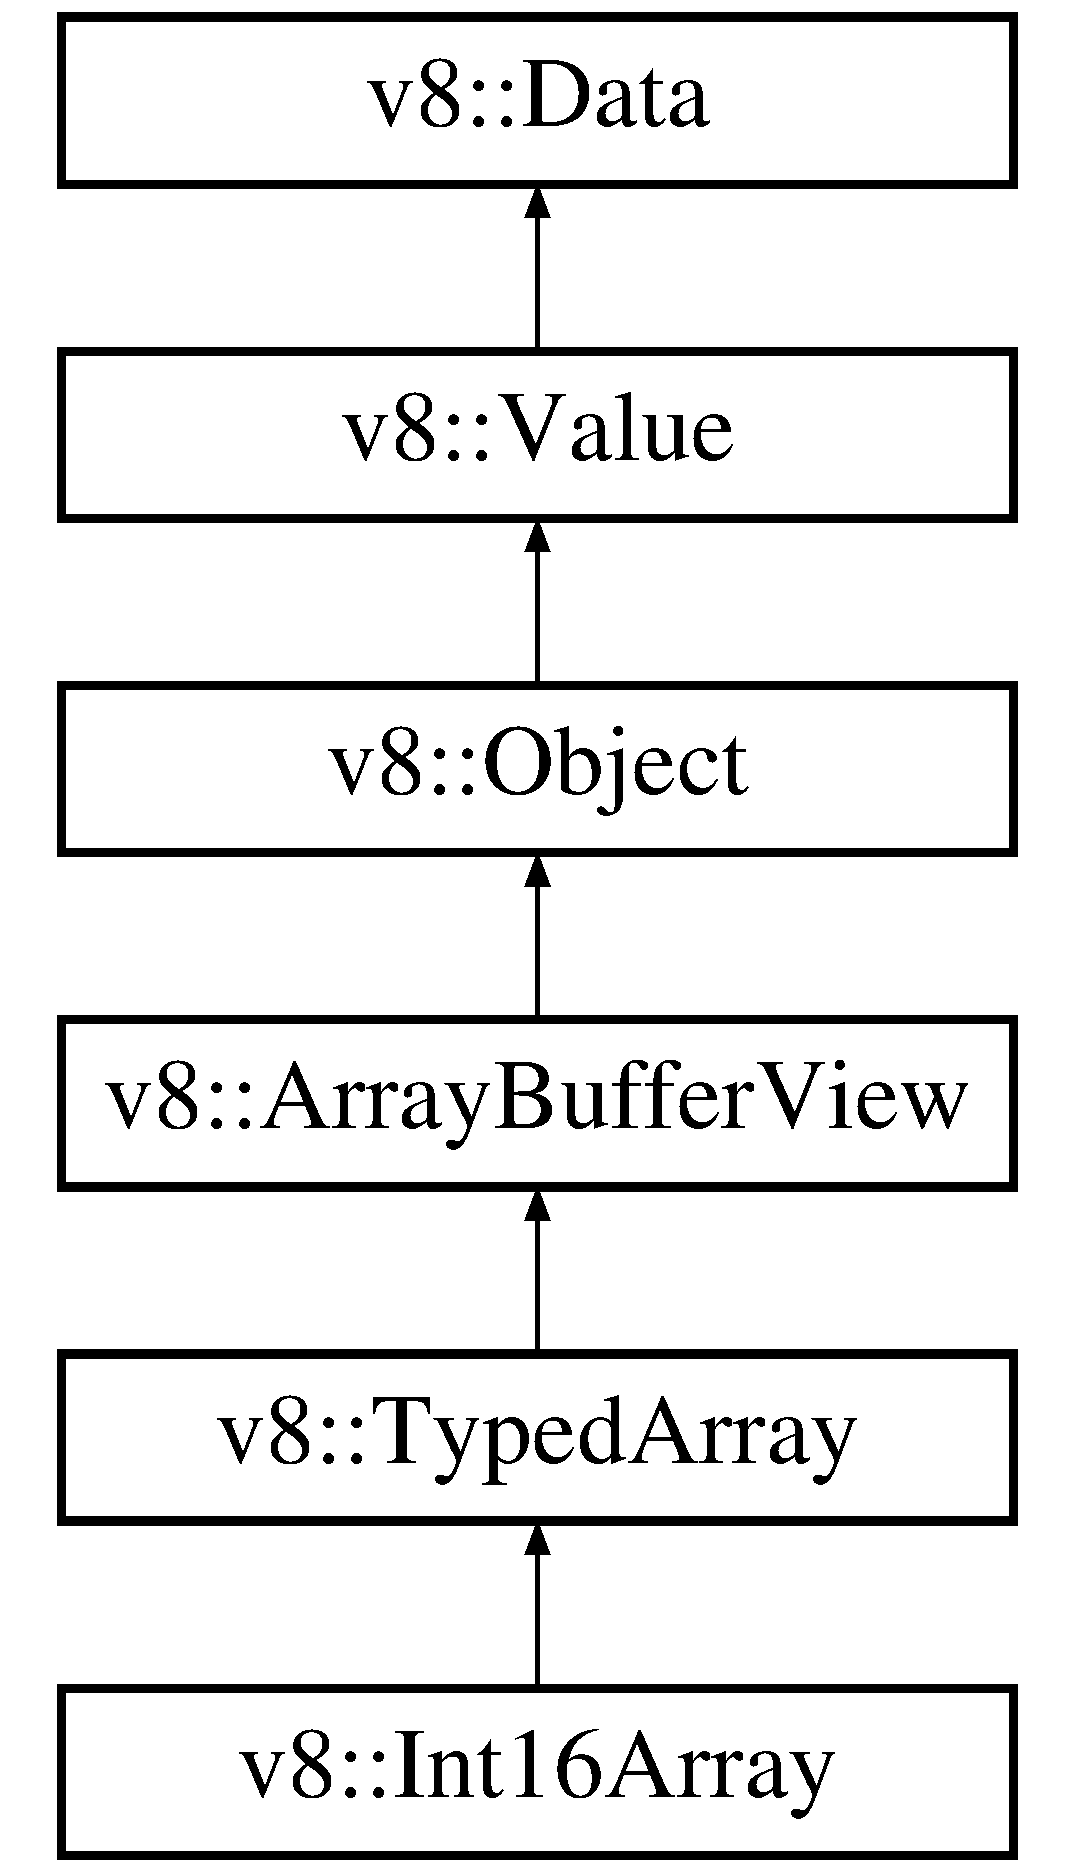
\includegraphics[height=6.000000cm]{classv8_1_1_int16_array}
\end{center}
\end{figure}
\subsection*{Static Public Member Functions}
\begin{DoxyCompactItemize}
\item 
static \hyperlink{classv8_1_1_local}{Local}$<$ \hyperlink{classv8_1_1_int16_array}{Int16\+Array} $>$ {\bfseries New} (\hyperlink{classv8_1_1_local}{Local}$<$ \hyperlink{classv8_1_1_array_buffer}{Array\+Buffer} $>$ array\+\_\+buffer, size\+\_\+t byte\+\_\+offset, size\+\_\+t length)\hypertarget{classv8_1_1_int16_array_a6e102d644c3f96345bcf212673b96090}{}\label{classv8_1_1_int16_array_a6e102d644c3f96345bcf212673b96090}

\item 
static \hyperlink{classv8_1_1_local}{Local}$<$ \hyperlink{classv8_1_1_int16_array}{Int16\+Array} $>$ {\bfseries New} (\hyperlink{classv8_1_1_local}{Local}$<$ \hyperlink{classv8_1_1_shared_array_buffer}{Shared\+Array\+Buffer} $>$ shared\+\_\+array\+\_\+buffer, size\+\_\+t byte\+\_\+offset, size\+\_\+t length)\hypertarget{classv8_1_1_int16_array_a9634021f52042c976091549358731432}{}\label{classv8_1_1_int16_array_a9634021f52042c976091549358731432}

\item 
static V8\+\_\+\+I\+N\+L\+I\+NE \hyperlink{classv8_1_1_int16_array}{Int16\+Array} $\ast$ {\bfseries Cast} (\hyperlink{classv8_1_1_value}{Value} $\ast$obj)\hypertarget{classv8_1_1_int16_array_abef12f11ace9c74a4ce451db28b954e5}{}\label{classv8_1_1_int16_array_abef12f11ace9c74a4ce451db28b954e5}

\end{DoxyCompactItemize}
\subsection*{Static Private Member Functions}
\begin{DoxyCompactItemize}
\item 
static void {\bfseries Check\+Cast} (\hyperlink{classv8_1_1_value}{Value} $\ast$obj)\hypertarget{classv8_1_1_int16_array_a893e79720d8b2fa2384a2daa36794769}{}\label{classv8_1_1_int16_array_a893e79720d8b2fa2384a2daa36794769}

\end{DoxyCompactItemize}
\subsection*{Additional Inherited Members}


\subsection{Detailed Description}
An instance of \hyperlink{classv8_1_1_int16_array}{Int16\+Array} constructor (E\+S6 draft 15.\+13.\+6). This A\+PI is experimental and may change significantly. 

The documentation for this class was generated from the following file\+:\begin{DoxyCompactItemize}
\item 
/\+Users/joshgav/node/v8/include/v8.\+h\end{DoxyCompactItemize}

\hypertarget{classv8_1_1_int32}{}\section{v8\+:\+:Int32 Class Reference}
\label{classv8_1_1_int32}\index{v8\+::\+Int32@{v8\+::\+Int32}}


{\ttfamily \#include $<$v8.\+h$>$}

Inheritance diagram for v8\+:\+:Int32\+:\begin{figure}[H]
\begin{center}
\leavevmode
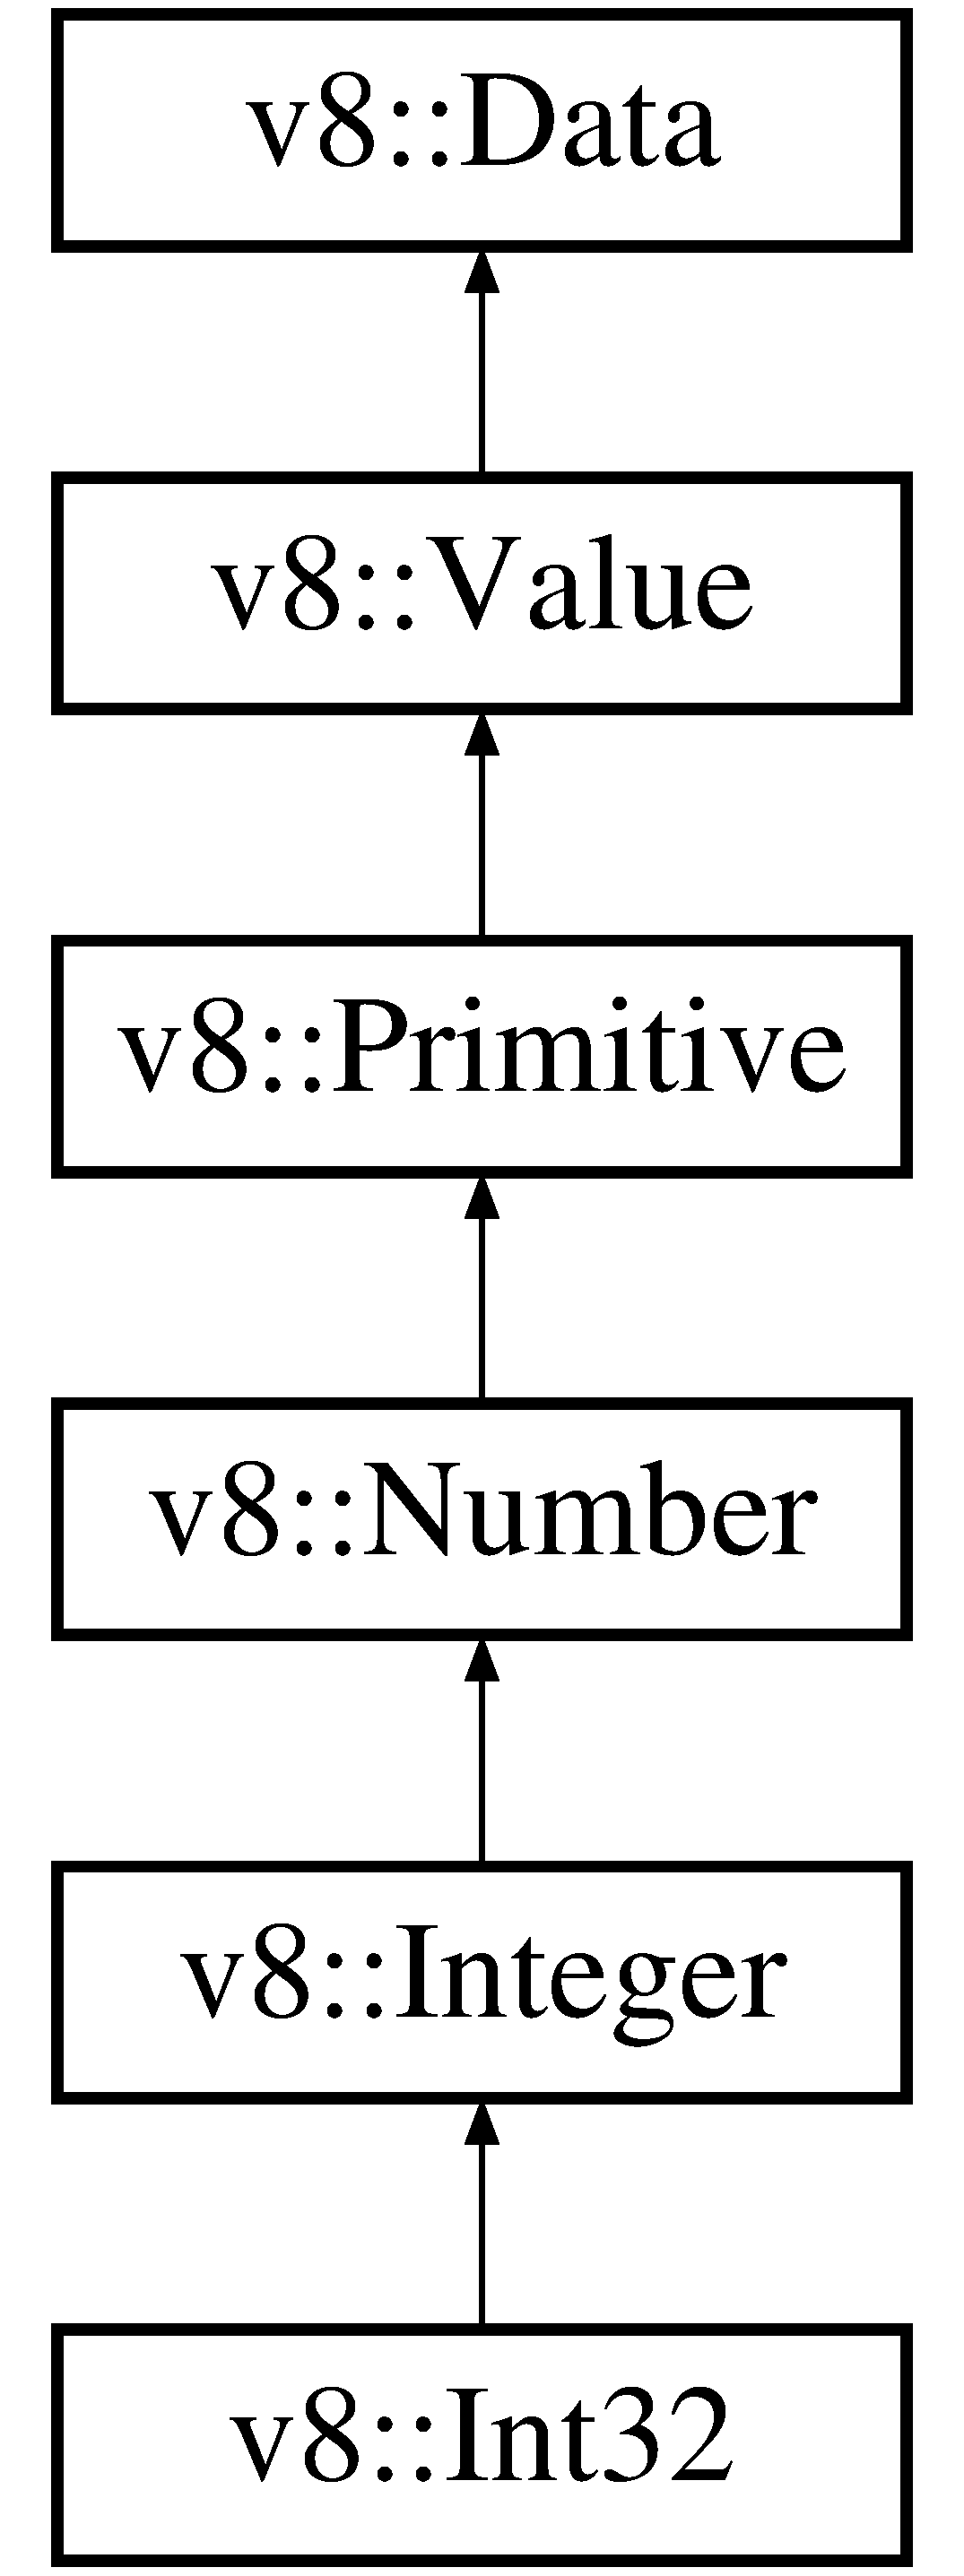
\includegraphics[height=6.000000cm]{classv8_1_1_int32}
\end{center}
\end{figure}
\subsection*{Public Member Functions}
\begin{DoxyCompactItemize}
\item 
int32\+\_\+t {\bfseries Value} () const \hypertarget{classv8_1_1_int32_a74860c6a524e1fb3f7b685ab0896be4b}{}\label{classv8_1_1_int32_a74860c6a524e1fb3f7b685ab0896be4b}

\end{DoxyCompactItemize}
\subsection*{Static Public Member Functions}
\begin{DoxyCompactItemize}
\item 
static V8\+\_\+\+I\+N\+L\+I\+NE \hyperlink{classv8_1_1_int32}{Int32} $\ast$ {\bfseries Cast} (\hyperlink{classv8_1_1_value}{v8\+::\+Value} $\ast$obj)\hypertarget{classv8_1_1_int32_a910c59c30a7f5f3c96afd0ba10d5339b}{}\label{classv8_1_1_int32_a910c59c30a7f5f3c96afd0ba10d5339b}

\end{DoxyCompactItemize}
\subsection*{Static Private Member Functions}
\begin{DoxyCompactItemize}
\item 
static void {\bfseries Check\+Cast} (\hyperlink{classv8_1_1_value}{v8\+::\+Value} $\ast$obj)\hypertarget{classv8_1_1_int32_a950badcc6761d8a92a8daf7e20bc40ff}{}\label{classv8_1_1_int32_a950badcc6761d8a92a8daf7e20bc40ff}

\end{DoxyCompactItemize}


\subsection{Detailed Description}
A Java\+Script value representing a 32-\/bit signed integer. 

The documentation for this class was generated from the following files\+:\begin{DoxyCompactItemize}
\item 
/\+Users/joshgav/node/v8/include/v8.\+h\item 
/\+Users/joshgav/node/v8/src/api.\+cc\end{DoxyCompactItemize}

\hypertarget{classv8_1_1_int32_array}{}\section{v8\+:\+:Int32\+Array Class Reference}
\label{classv8_1_1_int32_array}\index{v8\+::\+Int32\+Array@{v8\+::\+Int32\+Array}}


{\ttfamily \#include $<$v8.\+h$>$}

Inheritance diagram for v8\+:\+:Int32\+Array\+:\begin{figure}[H]
\begin{center}
\leavevmode
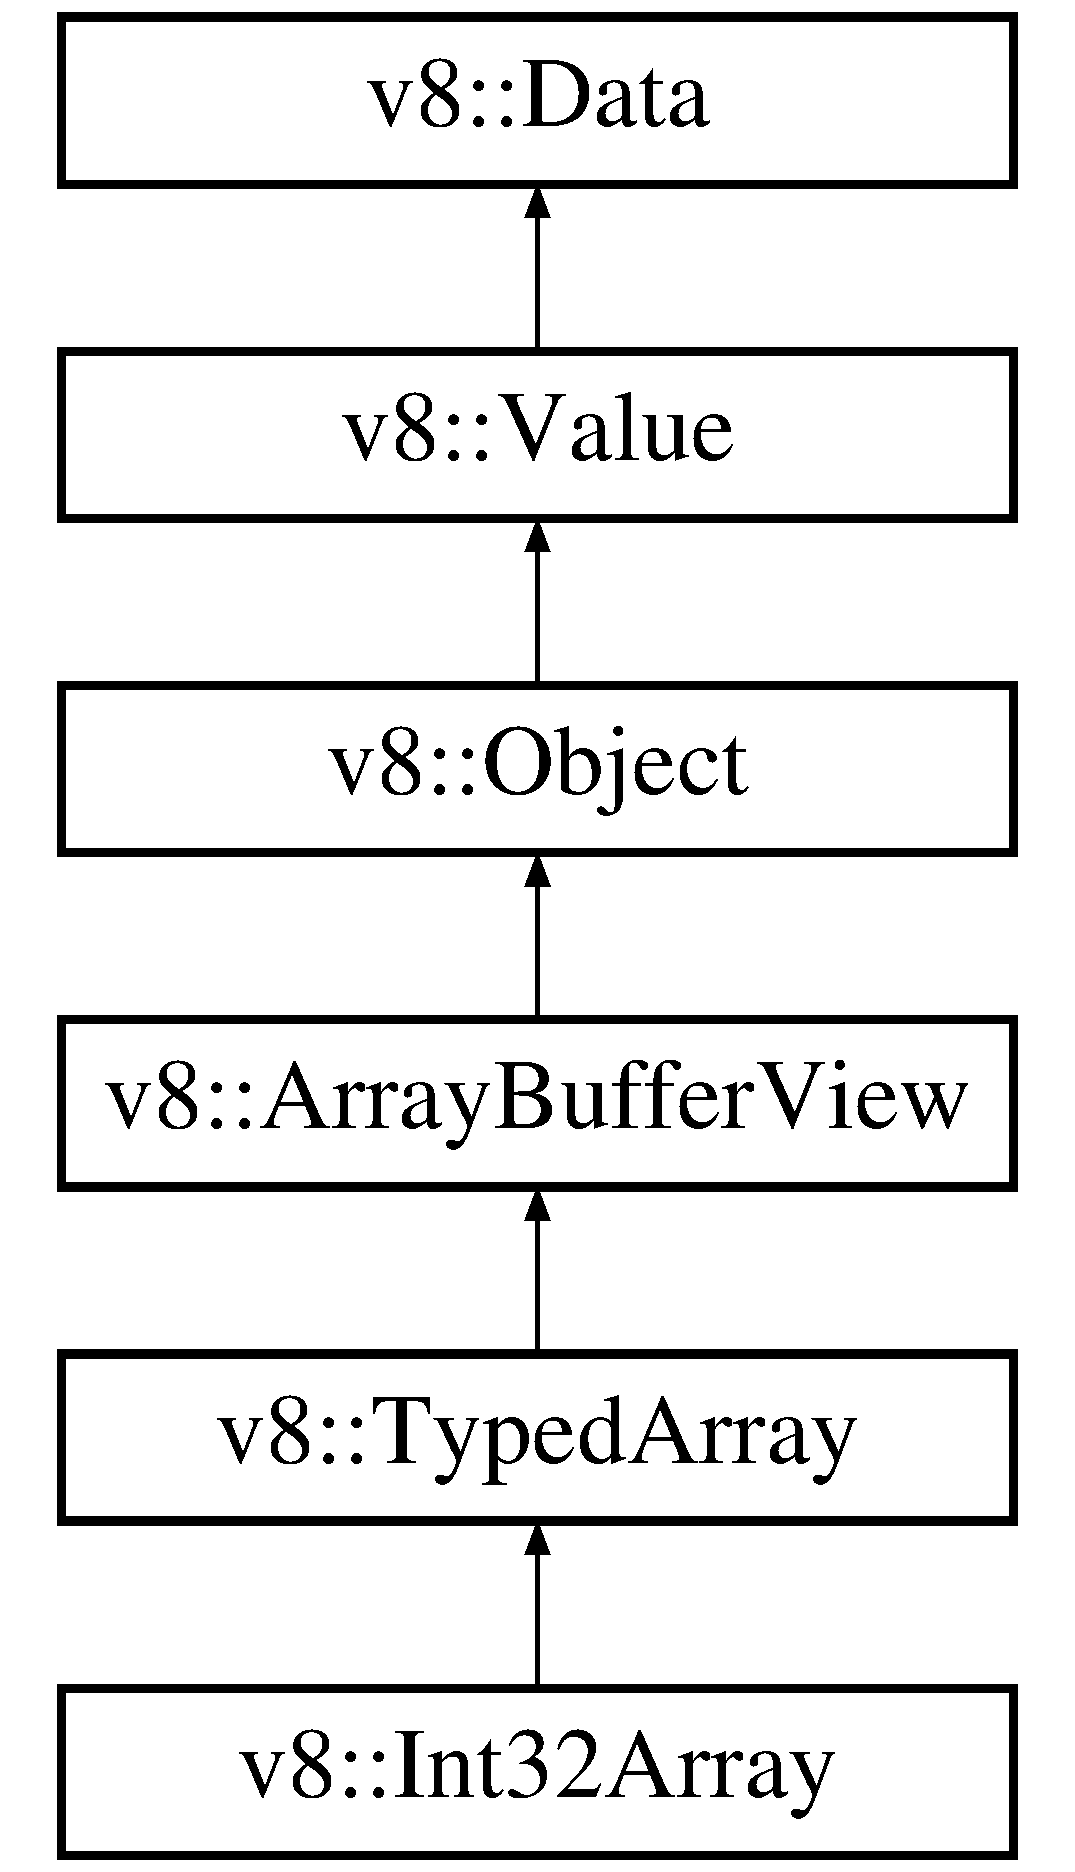
\includegraphics[height=6.000000cm]{classv8_1_1_int32_array}
\end{center}
\end{figure}
\subsection*{Static Public Member Functions}
\begin{DoxyCompactItemize}
\item 
static \hyperlink{classv8_1_1_local}{Local}$<$ \hyperlink{classv8_1_1_int32_array}{Int32\+Array} $>$ {\bfseries New} (\hyperlink{classv8_1_1_local}{Local}$<$ \hyperlink{classv8_1_1_array_buffer}{Array\+Buffer} $>$ array\+\_\+buffer, size\+\_\+t byte\+\_\+offset, size\+\_\+t length)\hypertarget{classv8_1_1_int32_array_a03adbd44725e3325d10bcc448e8bfd75}{}\label{classv8_1_1_int32_array_a03adbd44725e3325d10bcc448e8bfd75}

\item 
static \hyperlink{classv8_1_1_local}{Local}$<$ \hyperlink{classv8_1_1_int32_array}{Int32\+Array} $>$ {\bfseries New} (\hyperlink{classv8_1_1_local}{Local}$<$ \hyperlink{classv8_1_1_shared_array_buffer}{Shared\+Array\+Buffer} $>$ shared\+\_\+array\+\_\+buffer, size\+\_\+t byte\+\_\+offset, size\+\_\+t length)\hypertarget{classv8_1_1_int32_array_acf112fc9df4e0bf2791be73264779905}{}\label{classv8_1_1_int32_array_acf112fc9df4e0bf2791be73264779905}

\item 
static V8\+\_\+\+I\+N\+L\+I\+NE \hyperlink{classv8_1_1_int32_array}{Int32\+Array} $\ast$ {\bfseries Cast} (\hyperlink{classv8_1_1_value}{Value} $\ast$obj)\hypertarget{classv8_1_1_int32_array_afe7cdf534deadc3d872d8a43778809f1}{}\label{classv8_1_1_int32_array_afe7cdf534deadc3d872d8a43778809f1}

\end{DoxyCompactItemize}
\subsection*{Static Private Member Functions}
\begin{DoxyCompactItemize}
\item 
static void {\bfseries Check\+Cast} (\hyperlink{classv8_1_1_value}{Value} $\ast$obj)\hypertarget{classv8_1_1_int32_array_ab29d9e42a098d602e184deb555ba1757}{}\label{classv8_1_1_int32_array_ab29d9e42a098d602e184deb555ba1757}

\end{DoxyCompactItemize}
\subsection*{Additional Inherited Members}


\subsection{Detailed Description}
An instance of \hyperlink{classv8_1_1_int32_array}{Int32\+Array} constructor (E\+S6 draft 15.\+13.\+6). This A\+PI is experimental and may change significantly. 

The documentation for this class was generated from the following file\+:\begin{DoxyCompactItemize}
\item 
include/v8.\+h\end{DoxyCompactItemize}

\hypertarget{classv8_1_1_int8_array}{}\section{v8\+:\+:Int8\+Array Class Reference}
\label{classv8_1_1_int8_array}\index{v8\+::\+Int8\+Array@{v8\+::\+Int8\+Array}}


{\ttfamily \#include $<$v8.\+h$>$}

Inheritance diagram for v8\+:\+:Int8\+Array\+:\begin{figure}[H]
\begin{center}
\leavevmode
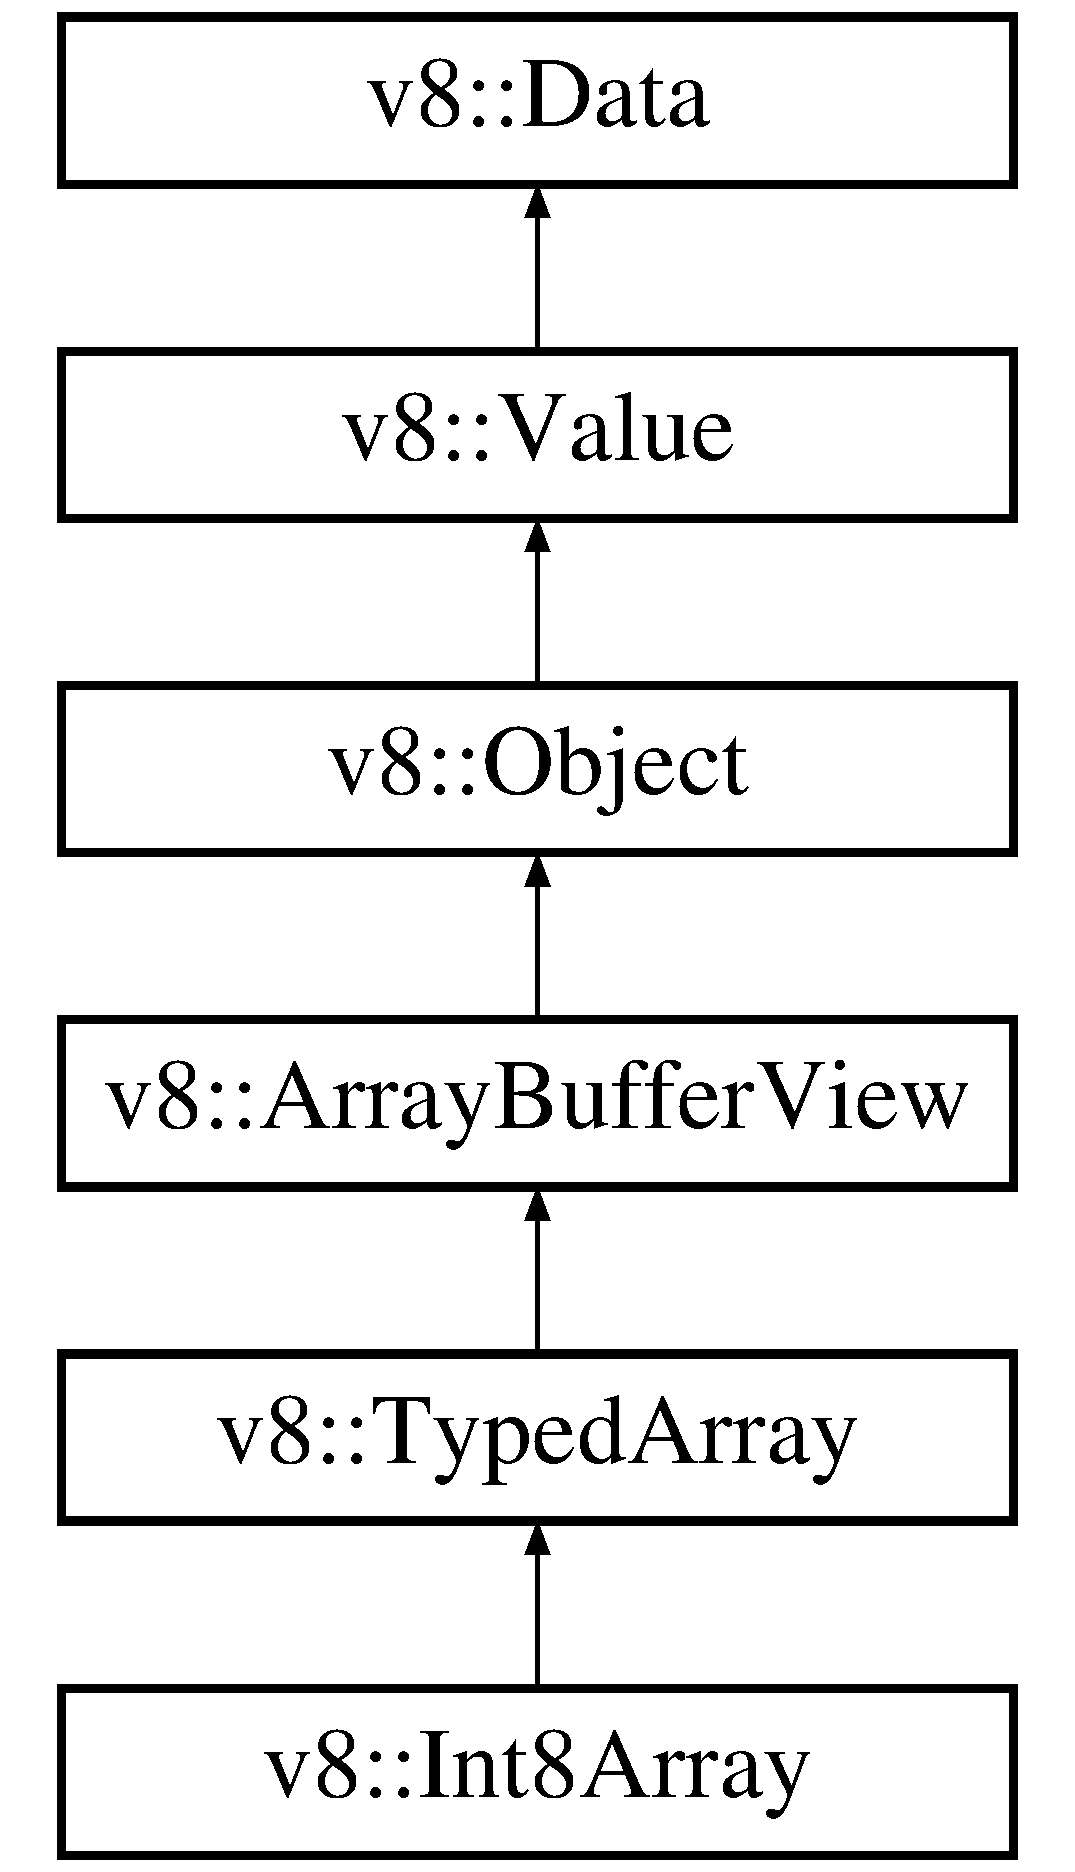
\includegraphics[height=6.000000cm]{classv8_1_1_int8_array}
\end{center}
\end{figure}
\subsection*{Static Public Member Functions}
\begin{DoxyCompactItemize}
\item 
static \hyperlink{classv8_1_1_local}{Local}$<$ \hyperlink{classv8_1_1_int8_array}{Int8\+Array} $>$ {\bfseries New} (\hyperlink{classv8_1_1_local}{Local}$<$ \hyperlink{classv8_1_1_array_buffer}{Array\+Buffer} $>$ array\+\_\+buffer, size\+\_\+t byte\+\_\+offset, size\+\_\+t length)\hypertarget{classv8_1_1_int8_array_a13e12d1a556aa2ef92271484a10acd21}{}\label{classv8_1_1_int8_array_a13e12d1a556aa2ef92271484a10acd21}

\item 
static \hyperlink{classv8_1_1_local}{Local}$<$ \hyperlink{classv8_1_1_int8_array}{Int8\+Array} $>$ {\bfseries New} (\hyperlink{classv8_1_1_local}{Local}$<$ \hyperlink{classv8_1_1_shared_array_buffer}{Shared\+Array\+Buffer} $>$ shared\+\_\+array\+\_\+buffer, size\+\_\+t byte\+\_\+offset, size\+\_\+t length)\hypertarget{classv8_1_1_int8_array_a364d52f1dc634e637321b2a9f9ec4dd8}{}\label{classv8_1_1_int8_array_a364d52f1dc634e637321b2a9f9ec4dd8}

\item 
static V8\+\_\+\+I\+N\+L\+I\+NE \hyperlink{classv8_1_1_int8_array}{Int8\+Array} $\ast$ {\bfseries Cast} (\hyperlink{classv8_1_1_value}{Value} $\ast$obj)\hypertarget{classv8_1_1_int8_array_a201a6b46e2cc455830d62c57bc8b4a3e}{}\label{classv8_1_1_int8_array_a201a6b46e2cc455830d62c57bc8b4a3e}

\end{DoxyCompactItemize}
\subsection*{Static Private Member Functions}
\begin{DoxyCompactItemize}
\item 
static void {\bfseries Check\+Cast} (\hyperlink{classv8_1_1_value}{Value} $\ast$obj)\hypertarget{classv8_1_1_int8_array_af584378c18f21b30fab6820ca0bd3c60}{}\label{classv8_1_1_int8_array_af584378c18f21b30fab6820ca0bd3c60}

\end{DoxyCompactItemize}
\subsection*{Additional Inherited Members}


\subsection{Detailed Description}
An instance of \hyperlink{classv8_1_1_int8_array}{Int8\+Array} constructor (E\+S6 draft 15.\+13.\+6). This A\+PI is experimental and may change significantly. 

The documentation for this class was generated from the following file\+:\begin{DoxyCompactItemize}
\item 
/\+Users/joshgav/node/v8/include/v8.\+h\end{DoxyCompactItemize}

\hypertarget{classv8_1_1_integer}{}\section{v8\+:\+:Integer Class Reference}
\label{classv8_1_1_integer}\index{v8\+::\+Integer@{v8\+::\+Integer}}


{\ttfamily \#include $<$v8.\+h$>$}

Inheritance diagram for v8\+:\+:Integer\+:\begin{figure}[H]
\begin{center}
\leavevmode
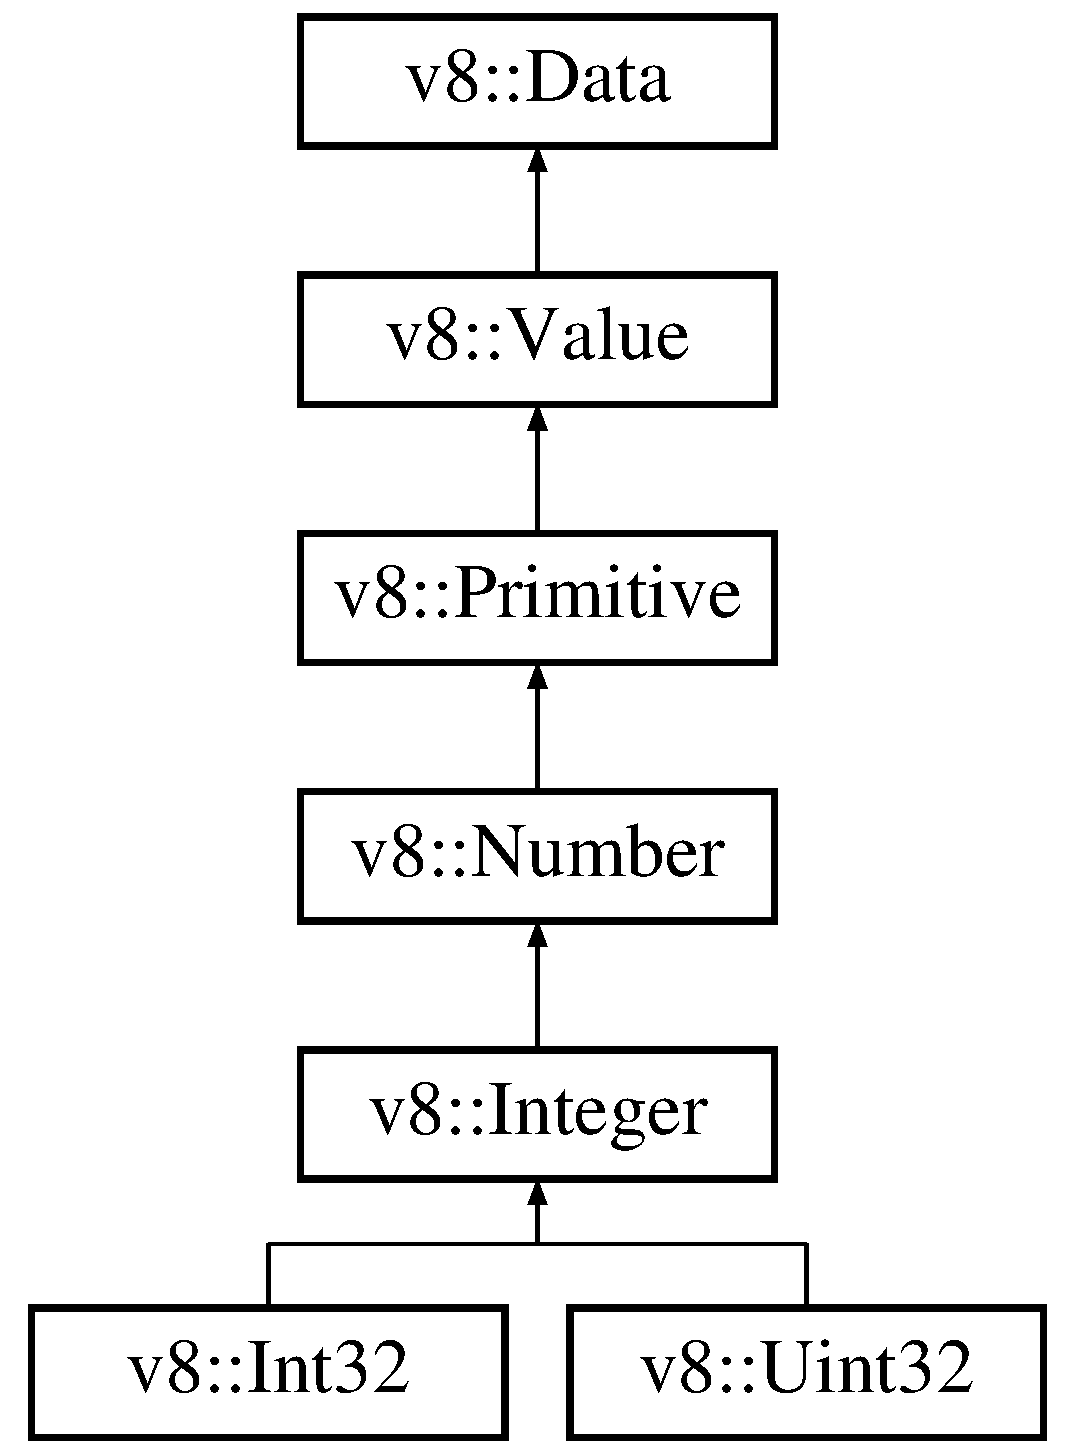
\includegraphics[height=6.000000cm]{classv8_1_1_integer}
\end{center}
\end{figure}
\subsection*{Public Member Functions}
\begin{DoxyCompactItemize}
\item 
int64\+\_\+t {\bfseries Value} () const \hypertarget{classv8_1_1_integer_a93bcfb39090631a3ff95843463183c9c}{}\label{classv8_1_1_integer_a93bcfb39090631a3ff95843463183c9c}

\end{DoxyCompactItemize}
\subsection*{Static Public Member Functions}
\begin{DoxyCompactItemize}
\item 
static \hyperlink{classv8_1_1_local}{Local}$<$ \hyperlink{classv8_1_1_integer}{Integer} $>$ {\bfseries New} (\hyperlink{classv8_1_1_isolate}{Isolate} $\ast$isolate, int32\+\_\+t value)\hypertarget{classv8_1_1_integer_a730d6e093c16d95edb5b92a4d05773d0}{}\label{classv8_1_1_integer_a730d6e093c16d95edb5b92a4d05773d0}

\item 
static \hyperlink{classv8_1_1_local}{Local}$<$ \hyperlink{classv8_1_1_integer}{Integer} $>$ {\bfseries New\+From\+Unsigned} (\hyperlink{classv8_1_1_isolate}{Isolate} $\ast$isolate, uint32\+\_\+t value)\hypertarget{classv8_1_1_integer_a6fbd6e79db802c737cb0bd5a259f134b}{}\label{classv8_1_1_integer_a6fbd6e79db802c737cb0bd5a259f134b}

\item 
static V8\+\_\+\+I\+N\+L\+I\+NE \hyperlink{classv8_1_1_integer}{Integer} $\ast$ {\bfseries Cast} (\hyperlink{classv8_1_1_value}{v8\+::\+Value} $\ast$obj)\hypertarget{classv8_1_1_integer_a886f73d3d8bb91f8235f66d8dccec12a}{}\label{classv8_1_1_integer_a886f73d3d8bb91f8235f66d8dccec12a}

\end{DoxyCompactItemize}
\subsection*{Static Private Member Functions}
\begin{DoxyCompactItemize}
\item 
static void {\bfseries Check\+Cast} (\hyperlink{classv8_1_1_value}{v8\+::\+Value} $\ast$obj)\hypertarget{classv8_1_1_integer_acc356589ec9cdb5a1dd232ed80e13a74}{}\label{classv8_1_1_integer_acc356589ec9cdb5a1dd232ed80e13a74}

\end{DoxyCompactItemize}


\subsection{Detailed Description}
A Java\+Script value representing a signed integer. 

The documentation for this class was generated from the following file\+:\begin{DoxyCompactItemize}
\item 
include/v8.\+h\end{DoxyCompactItemize}

\hypertarget{classv8_1_1internal_1_1_internals}{}\section{v8\+:\+:internal\+:\+:Internals Class Reference}
\label{classv8_1_1internal_1_1_internals}\index{v8\+::internal\+::\+Internals@{v8\+::internal\+::\+Internals}}


{\ttfamily \#include $<$v8.\+h$>$}

\subsection*{Static Public Member Functions}
\begin{DoxyCompactItemize}
\item 
static V8\+\_\+\+E\+X\+P\+O\+RT void {\bfseries Check\+Initialized\+Impl} (\hyperlink{classv8_1_1_isolate}{v8\+::\+Isolate} $\ast$isolate)\hypertarget{classv8_1_1internal_1_1_internals_ac5141eba7a786f0fa9f6db658f25d4ba}{}\label{classv8_1_1internal_1_1_internals_ac5141eba7a786f0fa9f6db658f25d4ba}

\item 
static V8\+\_\+\+I\+N\+L\+I\+NE void {\bfseries Check\+Initialized} (\hyperlink{classv8_1_1_isolate}{v8\+::\+Isolate} $\ast$isolate)\hypertarget{classv8_1_1internal_1_1_internals_a1aa4bc86bc011f055fe27d18e0849b8c}{}\label{classv8_1_1internal_1_1_internals_a1aa4bc86bc011f055fe27d18e0849b8c}

\item 
static V8\+\_\+\+I\+N\+L\+I\+NE bool {\bfseries Has\+Heap\+Object\+Tag} (const internal\+::\+Object $\ast$value)\hypertarget{classv8_1_1internal_1_1_internals_aece7d6117172e0ded0d21774e460cc28}{}\label{classv8_1_1internal_1_1_internals_aece7d6117172e0ded0d21774e460cc28}

\item 
static V8\+\_\+\+I\+N\+L\+I\+NE int {\bfseries Smi\+Value} (const internal\+::\+Object $\ast$value)\hypertarget{classv8_1_1internal_1_1_internals_ad00a8fac1a3b75795d4036eae8e8ccfb}{}\label{classv8_1_1internal_1_1_internals_ad00a8fac1a3b75795d4036eae8e8ccfb}

\item 
static V8\+\_\+\+I\+N\+L\+I\+NE internal\+::\+Object $\ast$ {\bfseries Int\+To\+Smi} (int value)\hypertarget{classv8_1_1internal_1_1_internals_a9e5ab52581c9c32ac018fb1cc98ab5fa}{}\label{classv8_1_1internal_1_1_internals_a9e5ab52581c9c32ac018fb1cc98ab5fa}

\item 
static V8\+\_\+\+I\+N\+L\+I\+NE bool {\bfseries Is\+Valid\+Smi} (intptr\+\_\+t value)\hypertarget{classv8_1_1internal_1_1_internals_a69b0abda8cf242042f4f19bcba35fd18}{}\label{classv8_1_1internal_1_1_internals_a69b0abda8cf242042f4f19bcba35fd18}

\item 
static V8\+\_\+\+I\+N\+L\+I\+NE int {\bfseries Get\+Instance\+Type} (const internal\+::\+Object $\ast$obj)\hypertarget{classv8_1_1internal_1_1_internals_a38c4f83c21a6e6620b515e569900afaa}{}\label{classv8_1_1internal_1_1_internals_a38c4f83c21a6e6620b515e569900afaa}

\item 
static V8\+\_\+\+I\+N\+L\+I\+NE int {\bfseries Get\+Oddball\+Kind} (const internal\+::\+Object $\ast$obj)\hypertarget{classv8_1_1internal_1_1_internals_a815059bbe1e7f23df55afed06d591b9a}{}\label{classv8_1_1internal_1_1_internals_a815059bbe1e7f23df55afed06d591b9a}

\item 
static V8\+\_\+\+I\+N\+L\+I\+NE bool {\bfseries Is\+External\+Two\+Byte\+String} (int instance\+\_\+type)\hypertarget{classv8_1_1internal_1_1_internals_afbf930e9dfde745b54e1e7e03b5b96c8}{}\label{classv8_1_1internal_1_1_internals_afbf930e9dfde745b54e1e7e03b5b96c8}

\item 
static V8\+\_\+\+I\+N\+L\+I\+NE uint8\+\_\+t {\bfseries Get\+Node\+Flag} (internal\+::\+Object $\ast$$\ast$obj, int shift)\hypertarget{classv8_1_1internal_1_1_internals_aa7df51a3da3e021e2bd4426461e6d1fb}{}\label{classv8_1_1internal_1_1_internals_aa7df51a3da3e021e2bd4426461e6d1fb}

\item 
static V8\+\_\+\+I\+N\+L\+I\+NE void {\bfseries Update\+Node\+Flag} (internal\+::\+Object $\ast$$\ast$obj, bool value, int shift)\hypertarget{classv8_1_1internal_1_1_internals_a868ffed15d660ac6959597e45a353d6e}{}\label{classv8_1_1internal_1_1_internals_a868ffed15d660ac6959597e45a353d6e}

\item 
static V8\+\_\+\+I\+N\+L\+I\+NE uint8\+\_\+t {\bfseries Get\+Node\+State} (internal\+::\+Object $\ast$$\ast$obj)\hypertarget{classv8_1_1internal_1_1_internals_a76c388eb1d813144512b0af2d1c5ac7b}{}\label{classv8_1_1internal_1_1_internals_a76c388eb1d813144512b0af2d1c5ac7b}

\item 
static V8\+\_\+\+I\+N\+L\+I\+NE void {\bfseries Update\+Node\+State} (internal\+::\+Object $\ast$$\ast$obj, uint8\+\_\+t value)\hypertarget{classv8_1_1internal_1_1_internals_a0f37a58646403a6a39f925006a98a0d0}{}\label{classv8_1_1internal_1_1_internals_a0f37a58646403a6a39f925006a98a0d0}

\item 
static V8\+\_\+\+I\+N\+L\+I\+NE void {\bfseries Set\+Embedder\+Data} (\hyperlink{classv8_1_1_isolate}{v8\+::\+Isolate} $\ast$isolate, uint32\+\_\+t slot, void $\ast$data)\hypertarget{classv8_1_1internal_1_1_internals_abe73d79832edf012f30a94ccc4b293d2}{}\label{classv8_1_1internal_1_1_internals_abe73d79832edf012f30a94ccc4b293d2}

\item 
static V8\+\_\+\+I\+N\+L\+I\+NE void $\ast$ {\bfseries Get\+Embedder\+Data} (const \hyperlink{classv8_1_1_isolate}{v8\+::\+Isolate} $\ast$isolate, uint32\+\_\+t slot)\hypertarget{classv8_1_1internal_1_1_internals_ab53d3d4ef80770cb3e7d10effed86d10}{}\label{classv8_1_1internal_1_1_internals_ab53d3d4ef80770cb3e7d10effed86d10}

\item 
static V8\+\_\+\+I\+N\+L\+I\+NE internal\+::\+Object $\ast$$\ast$ {\bfseries Get\+Root} (\hyperlink{classv8_1_1_isolate}{v8\+::\+Isolate} $\ast$isolate, int index)\hypertarget{classv8_1_1internal_1_1_internals_aae733fd76f6f692f83a6ded4ac8f1571}{}\label{classv8_1_1internal_1_1_internals_aae733fd76f6f692f83a6ded4ac8f1571}

\item 
{\footnotesize template$<$typename T $>$ }\\static V8\+\_\+\+I\+N\+L\+I\+NE T {\bfseries Read\+Field} (const internal\+::\+Object $\ast$ptr, int offset)\hypertarget{classv8_1_1internal_1_1_internals_a62d4c79489a23c4e0598e3e2561ffdd8}{}\label{classv8_1_1internal_1_1_internals_a62d4c79489a23c4e0598e3e2561ffdd8}

\item 
{\footnotesize template$<$typename T $>$ }\\static V8\+\_\+\+I\+N\+L\+I\+NE T {\bfseries Read\+Embedder\+Data} (const \hyperlink{classv8_1_1_context}{v8\+::\+Context} $\ast$context, int index)\hypertarget{classv8_1_1internal_1_1_internals_a98cf4d5b60b963cc544cdd3aeda52335}{}\label{classv8_1_1internal_1_1_internals_a98cf4d5b60b963cc544cdd3aeda52335}

\end{DoxyCompactItemize}
\subsection*{Static Public Attributes}
\begin{DoxyCompactItemize}
\item 
static const int {\bfseries k\+Heap\+Object\+Map\+Offset} = 0\hypertarget{classv8_1_1internal_1_1_internals_a0902a596b5656b4592157eaacc020512}{}\label{classv8_1_1internal_1_1_internals_a0902a596b5656b4592157eaacc020512}

\item 
static const int {\bfseries k\+Map\+Instance\+Type\+And\+Bit\+Field\+Offset}
\item 
static const int {\bfseries k\+String\+Resource\+Offset} = 3 $\ast$ k\+Api\+Pointer\+Size\hypertarget{classv8_1_1internal_1_1_internals_a8c2b35069864f567ca0c571310dd90a1}{}\label{classv8_1_1internal_1_1_internals_a8c2b35069864f567ca0c571310dd90a1}

\item 
static const int {\bfseries k\+Oddball\+Kind\+Offset} = 5 $\ast$ k\+Api\+Pointer\+Size + sizeof(double)\hypertarget{classv8_1_1internal_1_1_internals_a98685d6861a07139720cd296f94f2b73}{}\label{classv8_1_1internal_1_1_internals_a98685d6861a07139720cd296f94f2b73}

\item 
static const int {\bfseries k\+Foreign\+Address\+Offset} = k\+Api\+Pointer\+Size\hypertarget{classv8_1_1internal_1_1_internals_ad4134449ee39b95e5ac035996aa7d66b}{}\label{classv8_1_1internal_1_1_internals_ad4134449ee39b95e5ac035996aa7d66b}

\item 
static const int {\bfseries k\+J\+S\+Object\+Header\+Size} = 3 $\ast$ k\+Api\+Pointer\+Size\hypertarget{classv8_1_1internal_1_1_internals_af8faf3ff3271d26bafa6ca0ea87e2a57}{}\label{classv8_1_1internal_1_1_internals_af8faf3ff3271d26bafa6ca0ea87e2a57}

\item 
static const int {\bfseries k\+Fixed\+Array\+Header\+Size} = 2 $\ast$ k\+Api\+Pointer\+Size\hypertarget{classv8_1_1internal_1_1_internals_a715ca62a5ddceac28d43c470db067675}{}\label{classv8_1_1internal_1_1_internals_a715ca62a5ddceac28d43c470db067675}

\item 
static const int {\bfseries k\+Context\+Header\+Size} = 2 $\ast$ k\+Api\+Pointer\+Size\hypertarget{classv8_1_1internal_1_1_internals_aa5187d7653158ef851c53594e6e63851}{}\label{classv8_1_1internal_1_1_internals_aa5187d7653158ef851c53594e6e63851}

\item 
static const int {\bfseries k\+Context\+Embedder\+Data\+Index} = 5\hypertarget{classv8_1_1internal_1_1_internals_afb65846499ec5f68172e4b2e8301a493}{}\label{classv8_1_1internal_1_1_internals_afb65846499ec5f68172e4b2e8301a493}

\item 
static const int {\bfseries k\+Full\+String\+Representation\+Mask} = 0x07\hypertarget{classv8_1_1internal_1_1_internals_a5c39a86b30463928ea719def66916507}{}\label{classv8_1_1internal_1_1_internals_a5c39a86b30463928ea719def66916507}

\item 
static const int {\bfseries k\+String\+Encoding\+Mask} = 0x4\hypertarget{classv8_1_1internal_1_1_internals_a1927ac3def13a57e03025e62ca46d1c5}{}\label{classv8_1_1internal_1_1_internals_a1927ac3def13a57e03025e62ca46d1c5}

\item 
static const int {\bfseries k\+External\+Two\+Byte\+Representation\+Tag} = 0x02\hypertarget{classv8_1_1internal_1_1_internals_a73faf917416d2519b65c7255e77a74ce}{}\label{classv8_1_1internal_1_1_internals_a73faf917416d2519b65c7255e77a74ce}

\item 
static const int {\bfseries k\+External\+One\+Byte\+Representation\+Tag} = 0x06\hypertarget{classv8_1_1internal_1_1_internals_ac789a0a139ccbacec0c5fb2d79427305}{}\label{classv8_1_1internal_1_1_internals_ac789a0a139ccbacec0c5fb2d79427305}

\item 
static const int {\bfseries k\+Isolate\+Embedder\+Data\+Offset} = 0 $\ast$ k\+Api\+Pointer\+Size\hypertarget{classv8_1_1internal_1_1_internals_ad722bf4760df09958cd1062db4a5524c}{}\label{classv8_1_1internal_1_1_internals_ad722bf4760df09958cd1062db4a5524c}

\item 
static const int {\bfseries k\+Amount\+Of\+External\+Allocated\+Memory\+Offset}
\item 
static const int {\bfseries k\+Amount\+Of\+External\+Allocated\+Memory\+At\+Last\+Global\+G\+C\+Offset}
\item 
static const int {\bfseries k\+Isolate\+Roots\+Offset}
\item 
static const int {\bfseries k\+Undefined\+Value\+Root\+Index} = 4\hypertarget{classv8_1_1internal_1_1_internals_a7281ff0eafed559e64613465b1a03296}{}\label{classv8_1_1internal_1_1_internals_a7281ff0eafed559e64613465b1a03296}

\item 
static const int {\bfseries k\+The\+Hole\+Value\+Root\+Index} = 5\hypertarget{classv8_1_1internal_1_1_internals_ac07a35d3efef0c107062b3eb88696e31}{}\label{classv8_1_1internal_1_1_internals_ac07a35d3efef0c107062b3eb88696e31}

\item 
static const int {\bfseries k\+Null\+Value\+Root\+Index} = 6\hypertarget{classv8_1_1internal_1_1_internals_ab311cf753ec5c968052bd83ef21e83f8}{}\label{classv8_1_1internal_1_1_internals_ab311cf753ec5c968052bd83ef21e83f8}

\item 
static const int {\bfseries k\+True\+Value\+Root\+Index} = 7\hypertarget{classv8_1_1internal_1_1_internals_a93abd58b178eca469bade28e68b5c59e}{}\label{classv8_1_1internal_1_1_internals_a93abd58b178eca469bade28e68b5c59e}

\item 
static const int {\bfseries k\+False\+Value\+Root\+Index} = 8\hypertarget{classv8_1_1internal_1_1_internals_a90b6837aa368bbe4ffd914e6f753b167}{}\label{classv8_1_1internal_1_1_internals_a90b6837aa368bbe4ffd914e6f753b167}

\item 
static const int {\bfseries k\+Empty\+String\+Root\+Index} = 9\hypertarget{classv8_1_1internal_1_1_internals_a6f669f3d98fe653b281b26be3bc0655a}{}\label{classv8_1_1internal_1_1_internals_a6f669f3d98fe653b281b26be3bc0655a}

\item 
static const int {\bfseries k\+External\+Allocation\+Limit} = 192 $\ast$ 1024 $\ast$ 1024\hypertarget{classv8_1_1internal_1_1_internals_aa88e5a295f86584aa3e90ebc1a6c4739}{}\label{classv8_1_1internal_1_1_internals_aa88e5a295f86584aa3e90ebc1a6c4739}

\item 
static const int {\bfseries k\+Node\+Class\+Id\+Offset} = 1 $\ast$ k\+Api\+Pointer\+Size\hypertarget{classv8_1_1internal_1_1_internals_af4fb6d499cb87f03031ad4d6be6bcd8f}{}\label{classv8_1_1internal_1_1_internals_af4fb6d499cb87f03031ad4d6be6bcd8f}

\item 
static const int {\bfseries k\+Node\+Flags\+Offset} = 1 $\ast$ k\+Api\+Pointer\+Size + 3\hypertarget{classv8_1_1internal_1_1_internals_aee5606f2a44d43d8dafe344e0bb753ef}{}\label{classv8_1_1internal_1_1_internals_aee5606f2a44d43d8dafe344e0bb753ef}

\item 
static const int {\bfseries k\+Node\+State\+Mask} = 0x7\hypertarget{classv8_1_1internal_1_1_internals_a853acc088978d38a5a69091cf857a46d}{}\label{classv8_1_1internal_1_1_internals_a853acc088978d38a5a69091cf857a46d}

\item 
static const int {\bfseries k\+Node\+State\+Is\+Weak\+Value} = 2\hypertarget{classv8_1_1internal_1_1_internals_a8a5d4cc92a6952c2a50922c77a606e68}{}\label{classv8_1_1internal_1_1_internals_a8a5d4cc92a6952c2a50922c77a606e68}

\item 
static const int {\bfseries k\+Node\+State\+Is\+Pending\+Value} = 3\hypertarget{classv8_1_1internal_1_1_internals_a843b53b17257ecd957eade0d9f21c5ab}{}\label{classv8_1_1internal_1_1_internals_a843b53b17257ecd957eade0d9f21c5ab}

\item 
static const int {\bfseries k\+Node\+State\+Is\+Near\+Death\+Value} = 4\hypertarget{classv8_1_1internal_1_1_internals_a18f3e757639b07bdabb8cda7dd4a8bdb}{}\label{classv8_1_1internal_1_1_internals_a18f3e757639b07bdabb8cda7dd4a8bdb}

\item 
static const int {\bfseries k\+Node\+Is\+Independent\+Shift} = 3\hypertarget{classv8_1_1internal_1_1_internals_a228b2b58c77c17bc512b92d9e3aea48b}{}\label{classv8_1_1internal_1_1_internals_a228b2b58c77c17bc512b92d9e3aea48b}

\item 
static const int {\bfseries k\+Node\+Is\+Partially\+Dependent\+Shift} = 4\hypertarget{classv8_1_1internal_1_1_internals_aeda4d6fc1bd10ca57398597f3bb496f3}{}\label{classv8_1_1internal_1_1_internals_aeda4d6fc1bd10ca57398597f3bb496f3}

\item 
static const int {\bfseries k\+Node\+Is\+Active\+Shift} = 4\hypertarget{classv8_1_1internal_1_1_internals_a34e042b2fa0c64f133d1605819678b36}{}\label{classv8_1_1internal_1_1_internals_a34e042b2fa0c64f133d1605819678b36}

\item 
static const int {\bfseries k\+J\+S\+Object\+Type} = 0xb7\hypertarget{classv8_1_1internal_1_1_internals_a56b7062df5d9a7df491137d4c3341bcc}{}\label{classv8_1_1internal_1_1_internals_a56b7062df5d9a7df491137d4c3341bcc}

\item 
static const int {\bfseries k\+J\+S\+Api\+Object\+Type} = 0xb6\hypertarget{classv8_1_1internal_1_1_internals_aef1693d7df34df433622fdb3e26767c8}{}\label{classv8_1_1internal_1_1_internals_aef1693d7df34df433622fdb3e26767c8}

\item 
static const int {\bfseries k\+First\+Nonstring\+Type} = 0x80\hypertarget{classv8_1_1internal_1_1_internals_a6f4a54927b01a11f444fb2f00b47ca1d}{}\label{classv8_1_1internal_1_1_internals_a6f4a54927b01a11f444fb2f00b47ca1d}

\item 
static const int {\bfseries k\+Oddball\+Type} = 0x83\hypertarget{classv8_1_1internal_1_1_internals_a13081e936f8c96472f1b1496c70d4dc1}{}\label{classv8_1_1internal_1_1_internals_a13081e936f8c96472f1b1496c70d4dc1}

\item 
static const int {\bfseries k\+Foreign\+Type} = 0x87\hypertarget{classv8_1_1internal_1_1_internals_a263195f36f9e8ee64af70dc267a85d55}{}\label{classv8_1_1internal_1_1_internals_a263195f36f9e8ee64af70dc267a85d55}

\item 
static const int {\bfseries k\+Undefined\+Oddball\+Kind} = 5\hypertarget{classv8_1_1internal_1_1_internals_a39072b9e0ffea4031f4a1c514208b20d}{}\label{classv8_1_1internal_1_1_internals_a39072b9e0ffea4031f4a1c514208b20d}

\item 
static const int {\bfseries k\+Null\+Oddball\+Kind} = 3\hypertarget{classv8_1_1internal_1_1_internals_a72243c5512cb5cab9d10b6f29e775180}{}\label{classv8_1_1internal_1_1_internals_a72243c5512cb5cab9d10b6f29e775180}

\item 
static const uint32\+\_\+t {\bfseries k\+Num\+Isolate\+Data\+Slots} = 4\hypertarget{classv8_1_1internal_1_1_internals_a258de87ae638f06a1deebccf4fd93c3f}{}\label{classv8_1_1internal_1_1_internals_a258de87ae638f06a1deebccf4fd93c3f}

\end{DoxyCompactItemize}


\subsection{Detailed Description}
This class exports constants and functionality from within \hyperlink{namespacev8}{v8} that is necessary to implement inline functions in the \hyperlink{namespacev8}{v8} api. Don\textquotesingle{}t depend on functions and constants defined here. 

\subsection{Member Data Documentation}
\index{v8\+::internal\+::\+Internals@{v8\+::internal\+::\+Internals}!k\+Amount\+Of\+External\+Allocated\+Memory\+At\+Last\+Global\+G\+C\+Offset@{k\+Amount\+Of\+External\+Allocated\+Memory\+At\+Last\+Global\+G\+C\+Offset}}
\index{k\+Amount\+Of\+External\+Allocated\+Memory\+At\+Last\+Global\+G\+C\+Offset@{k\+Amount\+Of\+External\+Allocated\+Memory\+At\+Last\+Global\+G\+C\+Offset}!v8\+::internal\+::\+Internals@{v8\+::internal\+::\+Internals}}
\subsubsection[{\texorpdfstring{k\+Amount\+Of\+External\+Allocated\+Memory\+At\+Last\+Global\+G\+C\+Offset}{kAmountOfExternalAllocatedMemoryAtLastGlobalGCOffset}}]{\setlength{\rightskip}{0pt plus 5cm}const int v8\+::internal\+::\+Internals\+::k\+Amount\+Of\+External\+Allocated\+Memory\+At\+Last\+Global\+G\+C\+Offset\hspace{0.3cm}{\ttfamily [static]}}\hypertarget{classv8_1_1internal_1_1_internals_a4839a352b8fc929d6f05028abe0db272}{}\label{classv8_1_1internal_1_1_internals_a4839a352b8fc929d6f05028abe0db272}
{\bfseries Initial value\+:}
\begin{DoxyCode}
=
      kAmountOfExternalAllocatedMemoryOffset + kApiInt64Size
\end{DoxyCode}
\index{v8\+::internal\+::\+Internals@{v8\+::internal\+::\+Internals}!k\+Amount\+Of\+External\+Allocated\+Memory\+Offset@{k\+Amount\+Of\+External\+Allocated\+Memory\+Offset}}
\index{k\+Amount\+Of\+External\+Allocated\+Memory\+Offset@{k\+Amount\+Of\+External\+Allocated\+Memory\+Offset}!v8\+::internal\+::\+Internals@{v8\+::internal\+::\+Internals}}
\subsubsection[{\texorpdfstring{k\+Amount\+Of\+External\+Allocated\+Memory\+Offset}{kAmountOfExternalAllocatedMemoryOffset}}]{\setlength{\rightskip}{0pt plus 5cm}const int v8\+::internal\+::\+Internals\+::k\+Amount\+Of\+External\+Allocated\+Memory\+Offset\hspace{0.3cm}{\ttfamily [static]}}\hypertarget{classv8_1_1internal_1_1_internals_a715b5e2c414c5efd35c5e01d4f2b9f85}{}\label{classv8_1_1internal_1_1_internals_a715b5e2c414c5efd35c5e01d4f2b9f85}
{\bfseries Initial value\+:}
\begin{DoxyCode}
=
      4 * kApiPointerSize
\end{DoxyCode}
\index{v8\+::internal\+::\+Internals@{v8\+::internal\+::\+Internals}!k\+Isolate\+Roots\+Offset@{k\+Isolate\+Roots\+Offset}}
\index{k\+Isolate\+Roots\+Offset@{k\+Isolate\+Roots\+Offset}!v8\+::internal\+::\+Internals@{v8\+::internal\+::\+Internals}}
\subsubsection[{\texorpdfstring{k\+Isolate\+Roots\+Offset}{kIsolateRootsOffset}}]{\setlength{\rightskip}{0pt plus 5cm}const int v8\+::internal\+::\+Internals\+::k\+Isolate\+Roots\+Offset\hspace{0.3cm}{\ttfamily [static]}}\hypertarget{classv8_1_1internal_1_1_internals_a3142f942a25203ce7fca0e9a4563c74d}{}\label{classv8_1_1internal_1_1_internals_a3142f942a25203ce7fca0e9a4563c74d}
{\bfseries Initial value\+:}
\begin{DoxyCode}
=
      kAmountOfExternalAllocatedMemoryAtLastGlobalGCOffset + kApiInt64Size +
      kApiPointerSize
\end{DoxyCode}
\index{v8\+::internal\+::\+Internals@{v8\+::internal\+::\+Internals}!k\+Map\+Instance\+Type\+And\+Bit\+Field\+Offset@{k\+Map\+Instance\+Type\+And\+Bit\+Field\+Offset}}
\index{k\+Map\+Instance\+Type\+And\+Bit\+Field\+Offset@{k\+Map\+Instance\+Type\+And\+Bit\+Field\+Offset}!v8\+::internal\+::\+Internals@{v8\+::internal\+::\+Internals}}
\subsubsection[{\texorpdfstring{k\+Map\+Instance\+Type\+And\+Bit\+Field\+Offset}{kMapInstanceTypeAndBitFieldOffset}}]{\setlength{\rightskip}{0pt plus 5cm}const int v8\+::internal\+::\+Internals\+::k\+Map\+Instance\+Type\+And\+Bit\+Field\+Offset\hspace{0.3cm}{\ttfamily [static]}}\hypertarget{classv8_1_1internal_1_1_internals_aeda3ec9bc2906bf6162b9cf3df9fd94a}{}\label{classv8_1_1internal_1_1_internals_aeda3ec9bc2906bf6162b9cf3df9fd94a}
{\bfseries Initial value\+:}
\begin{DoxyCode}
=
      1 * kApiPointerSize + kApiIntSize
\end{DoxyCode}


The documentation for this class was generated from the following file\+:\begin{DoxyCompactItemize}
\item 
/\+Users/joshgav/node/v8/include/v8.\+h\end{DoxyCompactItemize}

\hypertarget{classv8_1_1_isolate}{}\section{v8\+:\+:Isolate Class Reference}
\label{classv8_1_1_isolate}\index{v8\+::\+Isolate@{v8\+::\+Isolate}}


{\ttfamily \#include $<$v8.\+h$>$}

\subsection*{Classes}
\begin{DoxyCompactItemize}
\item 
class \hyperlink{classv8_1_1_isolate_1_1_allow_javascript_execution_scope}{Allow\+Javascript\+Execution\+Scope}
\item 
struct \hyperlink{structv8_1_1_isolate_1_1_create_params}{Create\+Params}
\item 
class \hyperlink{classv8_1_1_isolate_1_1_disallow_javascript_execution_scope}{Disallow\+Javascript\+Execution\+Scope}
\item 
class \hyperlink{classv8_1_1_isolate_1_1_scope}{Scope}
\item 
class \hyperlink{classv8_1_1_isolate_1_1_suppress_microtask_execution_scope}{Suppress\+Microtask\+Execution\+Scope}
\end{DoxyCompactItemize}
\subsection*{Public Types}
\begin{DoxyCompactItemize}
\item 
enum \hyperlink{classv8_1_1_isolate_a5ae00cc99d8aca148c6f5f9698c432c9}{Garbage\+Collection\+Type} \{ \\*
{\bfseries k\+Full\+Garbage\+Collection}, 
\\*
{\bfseries k\+Minor\+Garbage\+Collection}
 \}
\item 
enum \hyperlink{classv8_1_1_isolate_aed6909379c3f2820cb3084710b73385d}{Use\+Counter\+Feature} \{ \\*
{\bfseries k\+Use\+Asm} = 0, 
\\*
{\bfseries k\+Break\+Iterator} = 1, 
\\*
{\bfseries k\+Legacy\+Const} = 2, 
\\*
{\bfseries k\+Mark\+Deque\+Overflow} = 3, 
\\*
{\bfseries k\+Store\+Buffer\+Overflow} = 4, 
\\*
{\bfseries k\+Slots\+Buffer\+Overflow} = 5, 
\\*
{\bfseries k\+Object\+Observe} = 6, 
\\*
{\bfseries k\+Forced\+GC} = 7, 
\\*
{\bfseries k\+Sloppy\+Mode} = 8, 
\\*
{\bfseries k\+Strict\+Mode} = 9, 
\\*
{\bfseries k\+Strong\+Mode} = 10, 
\\*
{\bfseries k\+Reg\+Exp\+Prototype\+Sticky\+Getter} = 11, 
\\*
{\bfseries k\+Reg\+Exp\+Prototype\+To\+String} = 12, 
\\*
{\bfseries k\+Reg\+Exp\+Prototype\+Unicode\+Getter} = 13, 
\\*
{\bfseries k\+Intl\+V8\+Parse} = 14, 
\\*
{\bfseries k\+Intl\+Pattern} = 15, 
\\*
{\bfseries k\+Intl\+Resolved} = 16, 
\\*
{\bfseries k\+Promise\+Chain} = 17, 
\\*
{\bfseries k\+Promise\+Accept} = 18, 
\\*
{\bfseries k\+Promise\+Defer} = 19, 
\\*
{\bfseries k\+Html\+Comment\+In\+External\+Script} = 20, 
\\*
{\bfseries k\+Html\+Comment} = 21, 
\\*
{\bfseries k\+Sloppy\+Mode\+Block\+Scoped\+Function\+Redefinition} = 22, 
\\*
{\bfseries k\+For\+In\+Initializer} = 23, 
\\*
{\bfseries k\+Array\+Protector\+Dirtied} = 24, 
\\*
{\bfseries k\+Array\+Species\+Modified} = 25, 
\\*
{\bfseries k\+Array\+Prototype\+Constructor\+Modified} = 26, 
\\*
{\bfseries k\+Array\+Instance\+Proto\+Modified} = 27, 
\\*
{\bfseries k\+Array\+Instance\+Constructor\+Modified} = 28, 
\\*
{\bfseries k\+Legacy\+Function\+Declaration} = 29, 
\\*
{\bfseries k\+Reg\+Exp\+Prototype\+Source\+Getter} = 30, 
\\*
{\bfseries k\+Reg\+Exp\+Prototype\+Old\+Flag\+Getter} = 31, 
\\*
{\bfseries k\+Use\+Counter\+Feature\+Count}
 \}
\item 
typedef void($\ast$ {\bfseries Use\+Counter\+Callback}) (\hyperlink{classv8_1_1_isolate}{Isolate} $\ast$isolate, \hyperlink{classv8_1_1_isolate_aed6909379c3f2820cb3084710b73385d}{Use\+Counter\+Feature} feature)\hypertarget{classv8_1_1_isolate_a7537ead98ee88eec2976348ba992935c}{}\label{classv8_1_1_isolate_a7537ead98ee88eec2976348ba992935c}

\item 
typedef bool($\ast$ \hyperlink{classv8_1_1_isolate_aeb1d49e500d9521b42743a6a740271e2}{Abort\+On\+Uncaught\+Exception\+Callback}) (\hyperlink{classv8_1_1_isolate}{Isolate} $\ast$)
\item 
typedef void($\ast$ {\bfseries G\+C\+Callback}) (\hyperlink{classv8_1_1_isolate}{Isolate} $\ast$isolate, \hyperlink{namespacev8_ac109d6f27e0c0f9ef4e98bcf7a806cf2}{G\+C\+Type} type, \hyperlink{namespacev8_a247c37a849f4d6c293b9b16e94e1944b}{G\+C\+Callback\+Flags} flags)\hypertarget{classv8_1_1_isolate_aba82364e6057ee6df3fb896a7e972750}{}\label{classv8_1_1_isolate_aba82364e6057ee6df3fb896a7e972750}

\end{DoxyCompactItemize}
\subsection*{Public Member Functions}
\begin{DoxyCompactItemize}
\item 
void {\bfseries Set\+Abort\+On\+Uncaught\+Exception\+Callback} (\hyperlink{classv8_1_1_isolate_aeb1d49e500d9521b42743a6a740271e2}{Abort\+On\+Uncaught\+Exception\+Callback} callback)\hypertarget{classv8_1_1_isolate_afb7aad57eec61464b5a7c3816bae60be}{}\label{classv8_1_1_isolate_afb7aad57eec61464b5a7c3816bae60be}

\item 
void \hyperlink{classv8_1_1_isolate_ae1b8d5696ba55dd3412989811c44c373}{Memory\+Pressure\+Notification} (\hyperlink{namespacev8_ae0e9a25bf51e518585f555806e7dc7b9}{Memory\+Pressure\+Level} level)
\item 
void \hyperlink{classv8_1_1_isolate_aec80bb49b6b7647ff75e8f2cc9484ea3}{Enter} ()
\item 
void \hyperlink{classv8_1_1_isolate_a64a8503cafd00d1d2cadfbb0c2345054}{Exit} ()
\item 
void \hyperlink{classv8_1_1_isolate_a1a5a5762e4221aff8c6b10f9e3cec0af}{Dispose} ()
\item 
void \hyperlink{classv8_1_1_isolate_ac62ff53be40f5ecd74fc9e72451da115}{Discard\+Thread\+Specific\+Metadata} ()
\item 
V8\+\_\+\+I\+N\+L\+I\+NE void \hyperlink{classv8_1_1_isolate_a2ae968a7ff8a397f1ac09d32990883f6}{Set\+Data} (uint32\+\_\+t slot, void $\ast$data)
\item 
V8\+\_\+\+I\+N\+L\+I\+NE void $\ast$ \hyperlink{classv8_1_1_isolate_aed85b3c82bf69a60ecebc2558ab95083}{Get\+Data} (uint32\+\_\+t slot)
\item 
void \hyperlink{classv8_1_1_isolate_add32e78544edaf8946ed9b328167e5e4}{Get\+Heap\+Statistics} (\hyperlink{classv8_1_1_heap_statistics}{Heap\+Statistics} $\ast$heap\+\_\+statistics)
\item 
size\+\_\+t \hyperlink{classv8_1_1_isolate_ad948acf0892e677a95fbc743b63ca5fa}{Number\+Of\+Heap\+Spaces} ()
\item 
bool \hyperlink{classv8_1_1_isolate_a28ab96294ee07064cbba01e969b62cbc}{Get\+Heap\+Space\+Statistics} (\hyperlink{classv8_1_1_heap_space_statistics}{Heap\+Space\+Statistics} $\ast$space\+\_\+statistics, size\+\_\+t index)
\item 
size\+\_\+t \hyperlink{classv8_1_1_isolate_a170044cddf655345682cb3c9b4bd1788}{Number\+Of\+Tracked\+Heap\+Object\+Types} ()
\item 
bool \hyperlink{classv8_1_1_isolate_a677681d4c3abfc1bc2e8b50c23623e24}{Get\+Heap\+Object\+Statistics\+At\+Last\+GC} (\hyperlink{classv8_1_1_heap_object_statistics}{Heap\+Object\+Statistics} $\ast$object\+\_\+statistics, size\+\_\+t type\+\_\+index)
\item 
void \hyperlink{classv8_1_1_isolate_a8b173b48a477267ccd6c7d17c492b82e}{Get\+Stack\+Sample} (const \hyperlink{structv8_1_1_register_state}{Register\+State} \&state, void $\ast$$\ast$frames, size\+\_\+t frames\+\_\+limit, \hyperlink{structv8_1_1_sample_info}{Sample\+Info} $\ast$sample\+\_\+info)
\item 
V8\+\_\+\+I\+N\+L\+I\+NE int64\+\_\+t \hyperlink{classv8_1_1_isolate_aaeda5fa60961a3d9d476c46200e30711}{Adjust\+Amount\+Of\+External\+Allocated\+Memory} (int64\+\_\+t change\+\_\+in\+\_\+bytes)
\item 
\hyperlink{classv8_1_1_heap_profiler}{Heap\+Profiler} $\ast$ \hyperlink{classv8_1_1_isolate_a12f5bdacd2d2f62b1f5a22429a470ebb}{Get\+Heap\+Profiler} ()
\item 
\hyperlink{classv8_1_1_cpu_profiler}{Cpu\+Profiler} $\ast$ \hyperlink{classv8_1_1_isolate_a2e6874236fd37561b2263e011b1a714e}{Get\+Cpu\+Profiler} ()
\item 
bool \hyperlink{classv8_1_1_isolate_afb6bbd31a87d0999dbbe5402447690a9}{In\+Context} ()
\item 
\hyperlink{classv8_1_1_local}{Local}$<$ \hyperlink{classv8_1_1_context}{Context} $>$ \hyperlink{classv8_1_1_isolate_af68803b1b9fb0bf76107f56a7a762fac}{Get\+Current\+Context} ()
\item 
\hyperlink{classv8_1_1_isolate_adf1b08359e4162ee05caab23377dbc9d}{V8\+\_\+\+D\+E\+P\+R\+E\+C\+A\+T\+E\+\_\+\+S\+O\+ON} (\char`\"{}Calling context concept is not compatible with tail calls, and will be \char`\"{}\char`\"{}removed.\char`\"{}, Local$<$ \hyperlink{classv8_1_1_context}{Context} $>$ Get\+Calling\+Context())
\item 
\hyperlink{classv8_1_1_local}{Local}$<$ \hyperlink{classv8_1_1_context}{Context} $>$ \hyperlink{classv8_1_1_isolate_a05849e1b944a40051e063f799c79864c}{Get\+Entered\+Context} ()
\item 
\hyperlink{classv8_1_1_local}{Local}$<$ \hyperlink{classv8_1_1_value}{Value} $>$ \hyperlink{classv8_1_1_isolate_ad2d4dd42267c374a37b93df403ef11ac}{Throw\+Exception} (\hyperlink{classv8_1_1_local}{Local}$<$ \hyperlink{classv8_1_1_value}{Value} $>$ exception)
\item 
{\footnotesize template$<$typename T $>$ }\\void \hyperlink{classv8_1_1_isolate_ae4418cb238686a321aa406e90c72fab5}{Set\+Object\+Group\+Id} (const \hyperlink{classv8_1_1_persistent}{Persistent}$<$ T $>$ \&object, \hyperlink{classv8_1_1_unique_id}{Unique\+Id} id)
\item 
{\footnotesize template$<$typename T $>$ }\\void \hyperlink{classv8_1_1_isolate_a0f8484db111e967d70ea7551b3593ce6}{Set\+Reference\+From\+Group} (\hyperlink{classv8_1_1_unique_id}{Unique\+Id} id, const \hyperlink{classv8_1_1_persistent}{Persistent}$<$ T $>$ \&child)
\item 
{\footnotesize template$<$typename T , typename S $>$ }\\void \hyperlink{classv8_1_1_isolate_a055fc73d18747b96c51f00599cdd3ec1}{Set\+Reference} (const \hyperlink{classv8_1_1_persistent}{Persistent}$<$ T $>$ \&parent, const \hyperlink{classv8_1_1_persistent}{Persistent}$<$ S $>$ \&child)
\item 
void \hyperlink{classv8_1_1_isolate_a7acdd74d063c4cbdb373f59253b7b64c}{Add\+G\+C\+Prologue\+Callback} (G\+C\+Callback callback, \hyperlink{namespacev8_ac109d6f27e0c0f9ef4e98bcf7a806cf2}{G\+C\+Type} gc\+\_\+type\+\_\+filter=k\+G\+C\+Type\+All)
\item 
void \hyperlink{classv8_1_1_isolate_a7c424950b2bc9589fc676a9b38b27d63}{Remove\+G\+C\+Prologue\+Callback} (G\+C\+Callback callback)
\item 
void \hyperlink{classv8_1_1_isolate_a33569984c556a90ae380f96aa7a82fad}{Set\+Embedder\+Heap\+Tracer} (\hyperlink{classv8_1_1_embedder_heap_tracer}{Embedder\+Heap\+Tracer} $\ast$tracer)
\item 
void \hyperlink{classv8_1_1_isolate_abe7ab165a962dd4a944d9bc489f5d2cf}{Add\+G\+C\+Epilogue\+Callback} (G\+C\+Callback callback, \hyperlink{namespacev8_ac109d6f27e0c0f9ef4e98bcf7a806cf2}{G\+C\+Type} gc\+\_\+type\+\_\+filter=k\+G\+C\+Type\+All)
\item 
void \hyperlink{classv8_1_1_isolate_a059d51bc45cdd5f4821233170863a9ff}{Remove\+G\+C\+Epilogue\+Callback} (G\+C\+Callback callback)
\item 
void \hyperlink{classv8_1_1_isolate_ad212b2e0b66ff5d586cd79cfa0b555fb}{Terminate\+Execution} ()
\item 
bool \hyperlink{classv8_1_1_isolate_aee57283198c192e83afe5e7d12d42e85}{Is\+Execution\+Terminating} ()
\item 
void \hyperlink{classv8_1_1_isolate_a75cbe037e7657a7c7bd65e2edf0164d5}{Cancel\+Terminate\+Execution} ()
\item 
void \hyperlink{classv8_1_1_isolate_a971b6094ecc6c7f55eb6f58a71a8afd3}{Request\+Interrupt} (Interrupt\+Callback callback, void $\ast$data)
\item 
void \hyperlink{classv8_1_1_isolate_a59fe893ed7e9df52cef2d59b2d98ab23}{Request\+Garbage\+Collection\+For\+Testing} (\hyperlink{classv8_1_1_isolate_a5ae00cc99d8aca148c6f5f9698c432c9}{Garbage\+Collection\+Type} type)
\item 
void \hyperlink{classv8_1_1_isolate_a28bf18f2f6ed468ec97f59df682e73c1}{Set\+Event\+Logger} (Log\+Event\+Callback that)
\item 
void \hyperlink{classv8_1_1_isolate_a1affdbf27486aa4c6a1ecae9997de98e}{Add\+Before\+Call\+Entered\+Callback} (Before\+Call\+Entered\+Callback callback)
\item 
void \hyperlink{classv8_1_1_isolate_a92be6cf5ce1e7360843794cc1528369f}{Remove\+Before\+Call\+Entered\+Callback} (Before\+Call\+Entered\+Callback callback)
\item 
void \hyperlink{classv8_1_1_isolate_a89656ac26d523c31fbfdbb12fb32f078}{Add\+Call\+Completed\+Callback} (Call\+Completed\+Callback callback)
\item 
{\bfseries V8\+\_\+\+D\+E\+P\+R\+E\+C\+A\+T\+E\+\_\+\+S\+O\+ON} (\char`\"{}Use callback with parameter\char`\"{}, void \hyperlink{classv8_1_1_isolate_a89656ac26d523c31fbfdbb12fb32f078}{Add\+Call\+Completed\+Callback}(Deprecated\+Call\+Completed\+Callback callback))\hypertarget{classv8_1_1_isolate_ab025ed92093822d1ed87c7669c207b4e}{}\label{classv8_1_1_isolate_ab025ed92093822d1ed87c7669c207b4e}

\item 
void \hyperlink{classv8_1_1_isolate_a46f0a5d35f8b29030922bdb433c0dc4f}{Remove\+Call\+Completed\+Callback} (Call\+Completed\+Callback callback)
\item 
{\bfseries V8\+\_\+\+D\+E\+P\+R\+E\+C\+A\+T\+E\+\_\+\+S\+O\+ON} (\char`\"{}Use callback with parameter\char`\"{}, void \hyperlink{classv8_1_1_isolate_a46f0a5d35f8b29030922bdb433c0dc4f}{Remove\+Call\+Completed\+Callback}(                               Deprecated\+Call\+Completed\+Callback callback))\hypertarget{classv8_1_1_isolate_a4ba659f54c46de49b75c4ca41e55535c}{}\label{classv8_1_1_isolate_a4ba659f54c46de49b75c4ca41e55535c}

\item 
void \hyperlink{classv8_1_1_isolate_a702f0ba4e5dee8a98aeb92239d58784e}{Set\+Promise\+Reject\+Callback} (Promise\+Reject\+Callback callback)
\item 
void \hyperlink{classv8_1_1_isolate_ac3cbe2a1632eb863912640dcfc98b6c8}{Run\+Microtasks} ()
\item 
void \hyperlink{classv8_1_1_isolate_a79a222a1a662d08479d5a1880c6793c5}{Enqueue\+Microtask} (\hyperlink{classv8_1_1_local}{Local}$<$ \hyperlink{classv8_1_1_function}{Function} $>$ microtask)
\item 
void \hyperlink{classv8_1_1_isolate_ad4d6c7dfdfc6c1bc857841de7e9967c3}{Enqueue\+Microtask} (Microtask\+Callback microtask, void $\ast$data=N\+U\+LL)
\item 
void \hyperlink{classv8_1_1_isolate_a6bc2069413d88ad90e4c8bee0b9e4037}{Set\+Microtasks\+Policy} (\hyperlink{namespacev8_a2f183b102b3d1b7a30a805e8c53c04da}{Microtasks\+Policy} policy)
\item 
{\bfseries V8\+\_\+\+D\+E\+P\+R\+E\+C\+A\+T\+E\+\_\+\+S\+O\+ON} (\char`\"{}Use \hyperlink{classv8_1_1_isolate_a6bc2069413d88ad90e4c8bee0b9e4037}{Set\+Microtasks\+Policy}\char`\"{}, void Set\+Autorun\+Microtasks(bool autorun))\hypertarget{classv8_1_1_isolate_a46bdd3b0109fd0a981462a83b1fe366a}{}\label{classv8_1_1_isolate_a46bdd3b0109fd0a981462a83b1fe366a}

\item 
\hyperlink{namespacev8_a2f183b102b3d1b7a30a805e8c53c04da}{Microtasks\+Policy} \hyperlink{classv8_1_1_isolate_a65ccc10f75f9497b6baf9535cf3f30db}{Get\+Microtasks\+Policy} () const 
\item 
{\bfseries V8\+\_\+\+D\+E\+P\+R\+E\+C\+A\+T\+E\+\_\+\+S\+O\+ON} (\char`\"{}Use \hyperlink{classv8_1_1_isolate_a65ccc10f75f9497b6baf9535cf3f30db}{Get\+Microtasks\+Policy}\char`\"{}, bool Will\+Autorun\+Microtasks() const)\hypertarget{classv8_1_1_isolate_a5123e1c47b45af3cdf51d6f635fef1f0}{}\label{classv8_1_1_isolate_a5123e1c47b45af3cdf51d6f635fef1f0}

\item 
void \hyperlink{classv8_1_1_isolate_ae9c09d4763df6c3f06c686eebcce2834}{Add\+Microtasks\+Completed\+Callback} (Microtasks\+Completed\+Callback callback)
\item 
void \hyperlink{classv8_1_1_isolate_a0fdc58db0d44c5a8f427d809e1c0b604}{Remove\+Microtasks\+Completed\+Callback} (Microtasks\+Completed\+Callback callback)
\item 
void \hyperlink{classv8_1_1_isolate_ad608b24b2c1b49a97ed4f04500976166}{Set\+Use\+Counter\+Callback} (Use\+Counter\+Callback callback)
\item 
void \hyperlink{classv8_1_1_isolate_ab59a904591d417ebb3889b5fa507447b}{Set\+Counter\+Function} (Counter\+Lookup\+Callback)
\item 
void \hyperlink{classv8_1_1_isolate_afd624c7e429a061c1cd9e5959ce6ebf0}{Set\+Create\+Histogram\+Function} (Create\+Histogram\+Callback)
\item 
void {\bfseries Set\+Add\+Histogram\+Sample\+Function} (Add\+Histogram\+Sample\+Callback)\hypertarget{classv8_1_1_isolate_ae5c813518efe1cfaccd0262ad6ed2f82}{}\label{classv8_1_1_isolate_ae5c813518efe1cfaccd0262ad6ed2f82}

\item 
bool \hyperlink{classv8_1_1_isolate_aba794ed25d4fa8780b3a07c66a5e5d4a}{Idle\+Notification\+Deadline} (double deadline\+\_\+in\+\_\+seconds)
\item 
{\bfseries V8\+\_\+\+D\+E\+P\+R\+E\+C\+A\+T\+ED} (\char`\"{}use \hyperlink{classv8_1_1_isolate_aba794ed25d4fa8780b3a07c66a5e5d4a}{Idle\+Notification\+Deadline}()\char`\"{}, bool Idle\+Notification(int idle\+\_\+time\+\_\+in\+\_\+ms))\hypertarget{classv8_1_1_isolate_a2f204e8d3ff66d940ddc58da5a202003}{}\label{classv8_1_1_isolate_a2f204e8d3ff66d940ddc58da5a202003}

\item 
void \hyperlink{classv8_1_1_isolate_aaf446f4877e4707a93d2c406fffd9fd6}{Low\+Memory\+Notification} ()
\item 
int \hyperlink{classv8_1_1_isolate_a4b5216bbb1792211422aee575d02f442}{Context\+Disposed\+Notification} (bool dependant\+\_\+context=true)
\item 
void \hyperlink{classv8_1_1_isolate_afaa09b3cb3a20f53bdcdce4b154d928f}{Isolate\+In\+Foreground\+Notification} ()
\item 
void \hyperlink{classv8_1_1_isolate_a15c1ba9cdb3526a6439e7fddb292ee93}{Isolate\+In\+Background\+Notification} ()
\item 
void \hyperlink{classv8_1_1_isolate_a71d976355bf47eb2dd09cd5d1279a40d}{Set\+Jit\+Code\+Event\+Handler} (\hyperlink{namespacev8_a06f34fa4fa4cfc8518366808d1d461c1}{Jit\+Code\+Event\+Options} options, \hyperlink{namespacev8_a39243bc91e63d64d111452fdb98c4733}{Jit\+Code\+Event\+Handler} event\+\_\+handler)
\item 
void \hyperlink{classv8_1_1_isolate_addbbe14af7efb92999ac3944bc9ffed5}{Set\+Stack\+Limit} (uintptr\+\_\+t stack\+\_\+limit)
\item 
void \hyperlink{classv8_1_1_isolate_a46c7fb2282970530c32740d7e5999b22}{Get\+Code\+Range} (void $\ast$$\ast$start, size\+\_\+t $\ast$length\+\_\+in\+\_\+bytes)
\item 
void \hyperlink{classv8_1_1_isolate_a131f1e2e6a80618ac3c8c266a041851d}{Set\+Fatal\+Error\+Handler} (Fatal\+Error\+Callback that)
\item 
void \hyperlink{classv8_1_1_isolate_ad91199faf0a599c69539af01f5df44e9}{Set\+Allow\+Code\+Generation\+From\+Strings\+Callback} (\hyperlink{namespacev8_a521d909ec201742a1cb35d50a8e2a3c2}{Allow\+Code\+Generation\+From\+Strings\+Callback} callback)
\item 
bool \hyperlink{classv8_1_1_isolate_a603a9bc7860d7936bce2dd45829869c3}{Is\+Dead} ()
\item 
bool \hyperlink{classv8_1_1_isolate_a1aaf99c9ce853fdece7a3b8fc4df49d5}{Add\+Message\+Listener} (Message\+Callback that, \hyperlink{classv8_1_1_local}{Local}$<$ \hyperlink{classv8_1_1_value}{Value} $>$ data=\hyperlink{classv8_1_1_local}{Local}$<$ \hyperlink{classv8_1_1_value}{Value} $>$())
\item 
void \hyperlink{classv8_1_1_isolate_a0319e55b26ba3ac51d867b37b917a21f}{Remove\+Message\+Listeners} (Message\+Callback that)
\item 
void \hyperlink{classv8_1_1_isolate_ab9ef29fc049d82e0c33994632b4f6ba6}{Set\+Failed\+Access\+Check\+Callback\+Function} (Failed\+Access\+Check\+Callback)
\item 
void \hyperlink{classv8_1_1_isolate_a0ea70b9953abf15184a20eba6aab389f}{Set\+Capture\+Stack\+Trace\+For\+Uncaught\+Exceptions} (bool capture, int frame\+\_\+limit=10, \hyperlink{classv8_1_1_stack_trace_a9704e4a37949eb8eb8ccddbddf161492}{Stack\+Trace\+::\+Stack\+Trace\+Options} options=Stack\+Trace\+::k\+Overview)
\item 
void \hyperlink{classv8_1_1_isolate_a92b19c574b44f9d093d5d4dedc4515c9}{V8\+\_\+\+D\+E\+P\+R\+E\+C\+A\+T\+ED} (\char`\"{}Use a combination of \hyperlink{classv8_1_1_isolate_a971b6094ecc6c7f55eb6f58a71a8afd3}{Request\+Interrupt} and G\+C\+Callback instead\char`\"{}, Add\+Memory\+Allocation\+Callback(Memory\+Allocation\+Callback callback,                                                                                                                               Object\+Space space, Allocation\+Action action))
\item 
void \hyperlink{classv8_1_1_isolate_a5be9f95acfcd2acc552f0a3eb6b41887}{V8\+\_\+\+D\+E\+P\+R\+E\+C\+A\+T\+ED} (\char`\"{}Use a combination of \hyperlink{classv8_1_1_isolate_a971b6094ecc6c7f55eb6f58a71a8afd3}{Request\+Interrupt} and G\+C\+Callback instead\char`\"{}, Remove\+Memory\+Allocation\+Callback(Memory\+Allocation\+Callback callback))
\item 
void \hyperlink{classv8_1_1_isolate_a44d513b6426299de4c16e069958a723b}{Visit\+External\+Resources} (\hyperlink{classv8_1_1_external_resource_visitor}{External\+Resource\+Visitor} $\ast$visitor)
\item 
void \hyperlink{classv8_1_1_isolate_a8c60c4e0f61250a422ba2336dcd50a75}{Visit\+Handles\+With\+Class\+Ids} (\hyperlink{classv8_1_1_persistent_handle_visitor}{Persistent\+Handle\+Visitor} $\ast$visitor)
\item 
void \hyperlink{classv8_1_1_isolate_ac5a3ecbb7ef90476150a20904c522744}{Visit\+Handles\+For\+Partial\+Dependence} (\hyperlink{classv8_1_1_persistent_handle_visitor}{Persistent\+Handle\+Visitor} $\ast$visitor)
\item 
void \hyperlink{classv8_1_1_isolate_a4f821750a43d17e51778b281ce2c1fcd}{Visit\+Weak\+Handles} (\hyperlink{classv8_1_1_persistent_handle_visitor}{Persistent\+Handle\+Visitor} $\ast$visitor)
\end{DoxyCompactItemize}
\subsection*{Static Public Member Functions}
\begin{DoxyCompactItemize}
\item 
static \hyperlink{classv8_1_1_isolate}{Isolate} $\ast$ \hyperlink{classv8_1_1_isolate_abab88b427984481cb58c371f6cb30005}{New} (const \hyperlink{structv8_1_1_isolate_1_1_create_params}{Create\+Params} \&params)
\item 
static \hyperlink{classv8_1_1_isolate}{Isolate} $\ast$ \hyperlink{classv8_1_1_isolate_afd8c10d0f01e2ae43522c3ddf0bb053d}{Get\+Current} ()
\item 
static V8\+\_\+\+I\+N\+L\+I\+NE uint32\+\_\+t \hyperlink{classv8_1_1_isolate_a7060092fd45588f4085753b3da1b2c82}{Get\+Number\+Of\+Data\+Slots} ()
\end{DoxyCompactItemize}
\subsection*{Private Member Functions}
\begin{DoxyCompactItemize}
\item 
{\bfseries Isolate} (const \hyperlink{classv8_1_1_isolate}{Isolate} \&)\hypertarget{classv8_1_1_isolate_a979321fdbb883356189324cb273157b5}{}\label{classv8_1_1_isolate_a979321fdbb883356189324cb273157b5}

\item 
\hyperlink{classv8_1_1_isolate}{Isolate} \& {\bfseries operator=} (const \hyperlink{classv8_1_1_isolate}{Isolate} \&)\hypertarget{classv8_1_1_isolate_a6956413fd22aed96a31b8a5ffe075e62}{}\label{classv8_1_1_isolate_a6956413fd22aed96a31b8a5ffe075e62}

\item 
void $\ast$ {\bfseries operator new} (size\+\_\+t size)\hypertarget{classv8_1_1_isolate_a2e4a83509115f47018e9b24adb3496a6}{}\label{classv8_1_1_isolate_a2e4a83509115f47018e9b24adb3496a6}

\item 
void {\bfseries operator delete} (void $\ast$, size\+\_\+t)\hypertarget{classv8_1_1_isolate_a952adce6105528dff9fd48db6953a31a}{}\label{classv8_1_1_isolate_a952adce6105528dff9fd48db6953a31a}

\item 
void {\bfseries Set\+Object\+Group\+Id} (\hyperlink{classv8_1_1internal_1_1_object}{internal\+::\+Object} $\ast$$\ast$object, \hyperlink{classv8_1_1_unique_id}{Unique\+Id} id)\hypertarget{classv8_1_1_isolate_a19de4baa103e8b7b4266fba9563e0634}{}\label{classv8_1_1_isolate_a19de4baa103e8b7b4266fba9563e0634}

\item 
void {\bfseries Set\+Reference\+From\+Group} (\hyperlink{classv8_1_1_unique_id}{Unique\+Id} id, \hyperlink{classv8_1_1internal_1_1_object}{internal\+::\+Object} $\ast$$\ast$object)\hypertarget{classv8_1_1_isolate_ab3d68205008e21a4bdc5640cb313e6bd}{}\label{classv8_1_1_isolate_ab3d68205008e21a4bdc5640cb313e6bd}

\item 
void {\bfseries Set\+Reference} (\hyperlink{classv8_1_1internal_1_1_object}{internal\+::\+Object} $\ast$$\ast$parent, \hyperlink{classv8_1_1internal_1_1_object}{internal\+::\+Object} $\ast$$\ast$child)\hypertarget{classv8_1_1_isolate_ac3d2330d18a3aec1de8de6165364e685}{}\label{classv8_1_1_isolate_ac3d2330d18a3aec1de8de6165364e685}

\item 
void {\bfseries Report\+External\+Allocation\+Limit\+Reached} ()\hypertarget{classv8_1_1_isolate_a46368f020b87e91876ec06bfdb255911}{}\label{classv8_1_1_isolate_a46368f020b87e91876ec06bfdb255911}

\end{DoxyCompactItemize}
\subsection*{Friends}
\begin{DoxyCompactItemize}
\item 
{\footnotesize template$<$class K , class V , class Traits $>$ }\\class {\bfseries Persistent\+Value\+Map\+Base}\hypertarget{classv8_1_1_isolate_a08e2b8f164392d71811ce6cc134f33e3}{}\label{classv8_1_1_isolate_a08e2b8f164392d71811ce6cc134f33e3}

\end{DoxyCompactItemize}


\subsection{Detailed Description}
\hyperlink{classv8_1_1_isolate}{Isolate} represents an isolated instance of the \hyperlink{classv8_1_1_v8}{V8} engine. \hyperlink{classv8_1_1_v8}{V8} isolates have completely separate states. Objects from one isolate must not be used in other isolates. The embedder can create multiple isolates and use them in parallel in multiple threads. An isolate can be entered by at most one thread at any given time. The Locker/\+Unlocker A\+PI must be used to synchronize. 

\subsection{Member Typedef Documentation}
\index{v8\+::\+Isolate@{v8\+::\+Isolate}!Abort\+On\+Uncaught\+Exception\+Callback@{Abort\+On\+Uncaught\+Exception\+Callback}}
\index{Abort\+On\+Uncaught\+Exception\+Callback@{Abort\+On\+Uncaught\+Exception\+Callback}!v8\+::\+Isolate@{v8\+::\+Isolate}}
\subsubsection[{\texorpdfstring{Abort\+On\+Uncaught\+Exception\+Callback}{AbortOnUncaughtExceptionCallback}}]{\setlength{\rightskip}{0pt plus 5cm}typedef bool($\ast$ v8\+::\+Isolate\+::\+Abort\+On\+Uncaught\+Exception\+Callback) ({\bf Isolate} $\ast$)}\hypertarget{classv8_1_1_isolate_aeb1d49e500d9521b42743a6a740271e2}{}\label{classv8_1_1_isolate_aeb1d49e500d9521b42743a6a740271e2}
Custom callback used by embedders to help \hyperlink{classv8_1_1_v8}{V8} determine if it should abort when it throws and no internal handler is predicted to catch the exception. If --abort-\/on-\/uncaught-\/exception is used on the command line, then \hyperlink{classv8_1_1_v8}{V8} will abort if either\+:
\begin{DoxyItemize}
\item no custom callback is set.
\item the custom callback set returns true. Otherwise, the custom callback will not be called and \hyperlink{classv8_1_1_v8}{V8} will not abort. 
\end{DoxyItemize}

\subsection{Member Enumeration Documentation}
\index{v8\+::\+Isolate@{v8\+::\+Isolate}!Garbage\+Collection\+Type@{Garbage\+Collection\+Type}}
\index{Garbage\+Collection\+Type@{Garbage\+Collection\+Type}!v8\+::\+Isolate@{v8\+::\+Isolate}}
\subsubsection[{\texorpdfstring{Garbage\+Collection\+Type}{GarbageCollectionType}}]{\setlength{\rightskip}{0pt plus 5cm}enum {\bf v8\+::\+Isolate\+::\+Garbage\+Collection\+Type}}\hypertarget{classv8_1_1_isolate_a5ae00cc99d8aca148c6f5f9698c432c9}{}\label{classv8_1_1_isolate_a5ae00cc99d8aca148c6f5f9698c432c9}
Types of garbage collections that can be requested via Request\+Garbage\+Collection\+For\+Testing. \index{v8\+::\+Isolate@{v8\+::\+Isolate}!Use\+Counter\+Feature@{Use\+Counter\+Feature}}
\index{Use\+Counter\+Feature@{Use\+Counter\+Feature}!v8\+::\+Isolate@{v8\+::\+Isolate}}
\subsubsection[{\texorpdfstring{Use\+Counter\+Feature}{UseCounterFeature}}]{\setlength{\rightskip}{0pt plus 5cm}enum {\bf v8\+::\+Isolate\+::\+Use\+Counter\+Feature}}\hypertarget{classv8_1_1_isolate_aed6909379c3f2820cb3084710b73385d}{}\label{classv8_1_1_isolate_aed6909379c3f2820cb3084710b73385d}
Features reported via the Set\+Use\+Counter\+Callback callback. Do not change assigned numbers of existing items; add new features to the end of this list. 

\subsection{Member Function Documentation}
\index{v8\+::\+Isolate@{v8\+::\+Isolate}!Add\+Before\+Call\+Entered\+Callback@{Add\+Before\+Call\+Entered\+Callback}}
\index{Add\+Before\+Call\+Entered\+Callback@{Add\+Before\+Call\+Entered\+Callback}!v8\+::\+Isolate@{v8\+::\+Isolate}}
\subsubsection[{\texorpdfstring{Add\+Before\+Call\+Entered\+Callback(\+Before\+Call\+Entered\+Callback callback)}{AddBeforeCallEnteredCallback(BeforeCallEnteredCallback callback)}}]{\setlength{\rightskip}{0pt plus 5cm}void v8\+::\+Isolate\+::\+Add\+Before\+Call\+Entered\+Callback (
\begin{DoxyParamCaption}
\item[{Before\+Call\+Entered\+Callback}]{callback}
\end{DoxyParamCaption}
)}\hypertarget{classv8_1_1_isolate_a1affdbf27486aa4c6a1ecae9997de98e}{}\label{classv8_1_1_isolate_a1affdbf27486aa4c6a1ecae9997de98e}
Adds a callback to notify the host application right before a script is about to run. If a script re-\/enters the runtime during executing, the Before\+Call\+Entered\+Callback is invoked for each re-\/entrance. Executing scripts inside the callback will re-\/trigger the callback. \index{v8\+::\+Isolate@{v8\+::\+Isolate}!Add\+Call\+Completed\+Callback@{Add\+Call\+Completed\+Callback}}
\index{Add\+Call\+Completed\+Callback@{Add\+Call\+Completed\+Callback}!v8\+::\+Isolate@{v8\+::\+Isolate}}
\subsubsection[{\texorpdfstring{Add\+Call\+Completed\+Callback(\+Call\+Completed\+Callback callback)}{AddCallCompletedCallback(CallCompletedCallback callback)}}]{\setlength{\rightskip}{0pt plus 5cm}void v8\+::\+Isolate\+::\+Add\+Call\+Completed\+Callback (
\begin{DoxyParamCaption}
\item[{Call\+Completed\+Callback}]{callback}
\end{DoxyParamCaption}
)}\hypertarget{classv8_1_1_isolate_a89656ac26d523c31fbfdbb12fb32f078}{}\label{classv8_1_1_isolate_a89656ac26d523c31fbfdbb12fb32f078}
Adds a callback to notify the host application when a script finished running. If a script re-\/enters the runtime during executing, the Call\+Completed\+Callback is only invoked when the outer-\/most script execution ends. Executing scripts inside the callback do not trigger further callbacks. \index{v8\+::\+Isolate@{v8\+::\+Isolate}!Add\+G\+C\+Epilogue\+Callback@{Add\+G\+C\+Epilogue\+Callback}}
\index{Add\+G\+C\+Epilogue\+Callback@{Add\+G\+C\+Epilogue\+Callback}!v8\+::\+Isolate@{v8\+::\+Isolate}}
\subsubsection[{\texorpdfstring{Add\+G\+C\+Epilogue\+Callback(\+G\+C\+Callback callback, G\+C\+Type gc\+\_\+type\+\_\+filter=k\+G\+C\+Type\+All)}{AddGCEpilogueCallback(GCCallback callback, GCType gc_type_filter=kGCTypeAll)}}]{\setlength{\rightskip}{0pt plus 5cm}void v8\+::\+Isolate\+::\+Add\+G\+C\+Epilogue\+Callback (
\begin{DoxyParamCaption}
\item[{G\+C\+Callback}]{callback, }
\item[{{\bf G\+C\+Type}}]{gc\+\_\+type\+\_\+filter = {\ttfamily kGCTypeAll}}
\end{DoxyParamCaption}
)}\hypertarget{classv8_1_1_isolate_abe7ab165a962dd4a944d9bc489f5d2cf}{}\label{classv8_1_1_isolate_abe7ab165a962dd4a944d9bc489f5d2cf}
Enables the host application to receive a notification after a garbage collection. Allocations are allowed in the callback function, but the callback is not re-\/entrant\+: if the allocation inside it will trigger the garbage collection, the callback won\textquotesingle{}t be called again. It is possible to specify the G\+C\+Type filter for your callback. But it is not possible to register the same callback function two times with different G\+C\+Type filters. \index{v8\+::\+Isolate@{v8\+::\+Isolate}!Add\+G\+C\+Prologue\+Callback@{Add\+G\+C\+Prologue\+Callback}}
\index{Add\+G\+C\+Prologue\+Callback@{Add\+G\+C\+Prologue\+Callback}!v8\+::\+Isolate@{v8\+::\+Isolate}}
\subsubsection[{\texorpdfstring{Add\+G\+C\+Prologue\+Callback(\+G\+C\+Callback callback, G\+C\+Type gc\+\_\+type\+\_\+filter=k\+G\+C\+Type\+All)}{AddGCPrologueCallback(GCCallback callback, GCType gc_type_filter=kGCTypeAll)}}]{\setlength{\rightskip}{0pt plus 5cm}void v8\+::\+Isolate\+::\+Add\+G\+C\+Prologue\+Callback (
\begin{DoxyParamCaption}
\item[{G\+C\+Callback}]{callback, }
\item[{{\bf G\+C\+Type}}]{gc\+\_\+type\+\_\+filter = {\ttfamily kGCTypeAll}}
\end{DoxyParamCaption}
)}\hypertarget{classv8_1_1_isolate_a7acdd74d063c4cbdb373f59253b7b64c}{}\label{classv8_1_1_isolate_a7acdd74d063c4cbdb373f59253b7b64c}
Enables the host application to receive a notification before a garbage collection. Allocations are allowed in the callback function, but the callback is not re-\/entrant\+: if the allocation inside it will trigger the garbage collection, the callback won\textquotesingle{}t be called again. It is possible to specify the G\+C\+Type filter for your callback. But it is not possible to register the same callback function two times with different G\+C\+Type filters. \index{v8\+::\+Isolate@{v8\+::\+Isolate}!Add\+Message\+Listener@{Add\+Message\+Listener}}
\index{Add\+Message\+Listener@{Add\+Message\+Listener}!v8\+::\+Isolate@{v8\+::\+Isolate}}
\subsubsection[{\texorpdfstring{Add\+Message\+Listener(\+Message\+Callback that, Local$<$ Value $>$ data=\+Local$<$ Value $>$())}{AddMessageListener(MessageCallback that, Local< Value > data=Local< Value >())}}]{\setlength{\rightskip}{0pt plus 5cm}bool v8\+::\+Isolate\+::\+Add\+Message\+Listener (
\begin{DoxyParamCaption}
\item[{Message\+Callback}]{that, }
\item[{{\bf Local}$<$ {\bf Value} $>$}]{data = {\ttfamily {\bf Local}$<${\bf Value}$>$()}}
\end{DoxyParamCaption}
)}\hypertarget{classv8_1_1_isolate_a1aaf99c9ce853fdece7a3b8fc4df49d5}{}\label{classv8_1_1_isolate_a1aaf99c9ce853fdece7a3b8fc4df49d5}
Adds a message listener.

The same message listener can be added more than once and in that case it will be called more than once for each message.

If data is specified, it will be passed to the callback when it is called. Otherwise, the exception object will be passed to the callback instead. \index{v8\+::\+Isolate@{v8\+::\+Isolate}!Add\+Microtasks\+Completed\+Callback@{Add\+Microtasks\+Completed\+Callback}}
\index{Add\+Microtasks\+Completed\+Callback@{Add\+Microtasks\+Completed\+Callback}!v8\+::\+Isolate@{v8\+::\+Isolate}}
\subsubsection[{\texorpdfstring{Add\+Microtasks\+Completed\+Callback(\+Microtasks\+Completed\+Callback callback)}{AddMicrotasksCompletedCallback(MicrotasksCompletedCallback callback)}}]{\setlength{\rightskip}{0pt plus 5cm}void v8\+::\+Isolate\+::\+Add\+Microtasks\+Completed\+Callback (
\begin{DoxyParamCaption}
\item[{Microtasks\+Completed\+Callback}]{callback}
\end{DoxyParamCaption}
)}\hypertarget{classv8_1_1_isolate_ae9c09d4763df6c3f06c686eebcce2834}{}\label{classv8_1_1_isolate_ae9c09d4763df6c3f06c686eebcce2834}
Experimental\+: adds a callback to notify the host application after microtasks were run. The callback is triggered by explicit Run\+Microtasks call or automatic microtasks execution (see Set\+Autorun\+Microtasks).

Callback will trigger even if microtasks were attempted to run, but the microtasks queue was empty and no single microtask was actually executed.

Executing scriptsinside the callback will not re-\/trigger microtasks and the callback. \index{v8\+::\+Isolate@{v8\+::\+Isolate}!Adjust\+Amount\+Of\+External\+Allocated\+Memory@{Adjust\+Amount\+Of\+External\+Allocated\+Memory}}
\index{Adjust\+Amount\+Of\+External\+Allocated\+Memory@{Adjust\+Amount\+Of\+External\+Allocated\+Memory}!v8\+::\+Isolate@{v8\+::\+Isolate}}
\subsubsection[{\texorpdfstring{Adjust\+Amount\+Of\+External\+Allocated\+Memory(int64\+\_\+t change\+\_\+in\+\_\+bytes)}{AdjustAmountOfExternalAllocatedMemory(int64_t change_in_bytes)}}]{\setlength{\rightskip}{0pt plus 5cm}int64\+\_\+t v8\+::\+Isolate\+::\+Adjust\+Amount\+Of\+External\+Allocated\+Memory (
\begin{DoxyParamCaption}
\item[{int64\+\_\+t}]{change\+\_\+in\+\_\+bytes}
\end{DoxyParamCaption}
)}\hypertarget{classv8_1_1_isolate_aaeda5fa60961a3d9d476c46200e30711}{}\label{classv8_1_1_isolate_aaeda5fa60961a3d9d476c46200e30711}
Adjusts the amount of registered external memory. Used to give \hyperlink{classv8_1_1_v8}{V8} an indication of the amount of externally allocated memory that is kept alive by Java\+Script objects. \hyperlink{classv8_1_1_v8}{V8} uses this to decide when to perform global garbage collections. Registering externally allocated memory will trigger global garbage collections more often than it would otherwise in an attempt to garbage collect the Java\+Script objects that keep the externally allocated memory alive.


\begin{DoxyParams}{Parameters}
{\em change\+\_\+in\+\_\+bytes} & the change in externally allocated memory that is kept alive by Java\+Script objects. \\
\hline
\end{DoxyParams}
\begin{DoxyReturn}{Returns}
the adjusted value. 
\end{DoxyReturn}
\index{v8\+::\+Isolate@{v8\+::\+Isolate}!Cancel\+Terminate\+Execution@{Cancel\+Terminate\+Execution}}
\index{Cancel\+Terminate\+Execution@{Cancel\+Terminate\+Execution}!v8\+::\+Isolate@{v8\+::\+Isolate}}
\subsubsection[{\texorpdfstring{Cancel\+Terminate\+Execution()}{CancelTerminateExecution()}}]{\setlength{\rightskip}{0pt plus 5cm}void v8\+::\+Isolate\+::\+Cancel\+Terminate\+Execution (
\begin{DoxyParamCaption}
{}
\end{DoxyParamCaption}
)}\hypertarget{classv8_1_1_isolate_a75cbe037e7657a7c7bd65e2edf0164d5}{}\label{classv8_1_1_isolate_a75cbe037e7657a7c7bd65e2edf0164d5}
Resume execution capability in the given isolate, whose execution was previously forcefully terminated using \hyperlink{classv8_1_1_isolate_ad212b2e0b66ff5d586cd79cfa0b555fb}{Terminate\+Execution()}.

When execution is forcefully terminated using \hyperlink{classv8_1_1_isolate_ad212b2e0b66ff5d586cd79cfa0b555fb}{Terminate\+Execution()}, the isolate can not resume execution until all Java\+Script frames have propagated the uncatchable exception which is generated. This method allows the program embedding the engine to handle the termination event and resume execution capability, even if Java\+Script frames remain on the stack.

This method can be used by any thread even if that thread has not acquired the \hyperlink{classv8_1_1_v8}{V8} lock with a \hyperlink{classv8_1_1_locker}{Locker} object. \index{v8\+::\+Isolate@{v8\+::\+Isolate}!Context\+Disposed\+Notification@{Context\+Disposed\+Notification}}
\index{Context\+Disposed\+Notification@{Context\+Disposed\+Notification}!v8\+::\+Isolate@{v8\+::\+Isolate}}
\subsubsection[{\texorpdfstring{Context\+Disposed\+Notification(bool dependant\+\_\+context=true)}{ContextDisposedNotification(bool dependant_context=true)}}]{\setlength{\rightskip}{0pt plus 5cm}int v8\+::\+Isolate\+::\+Context\+Disposed\+Notification (
\begin{DoxyParamCaption}
\item[{bool}]{dependant\+\_\+context = {\ttfamily true}}
\end{DoxyParamCaption}
)}\hypertarget{classv8_1_1_isolate_a4b5216bbb1792211422aee575d02f442}{}\label{classv8_1_1_isolate_a4b5216bbb1792211422aee575d02f442}
Optional notification that a context has been disposed. \hyperlink{classv8_1_1_v8}{V8} uses these notifications to guide the GC heuristic. Returns the number of context disposals -\/ including this one -\/ since the last time \hyperlink{classv8_1_1_v8}{V8} had a chance to clean up.

The optional parameter $\vert$dependant\+\_\+context$\vert$ specifies whether the disposed context was depending on state from other contexts or not. \index{v8\+::\+Isolate@{v8\+::\+Isolate}!Discard\+Thread\+Specific\+Metadata@{Discard\+Thread\+Specific\+Metadata}}
\index{Discard\+Thread\+Specific\+Metadata@{Discard\+Thread\+Specific\+Metadata}!v8\+::\+Isolate@{v8\+::\+Isolate}}
\subsubsection[{\texorpdfstring{Discard\+Thread\+Specific\+Metadata()}{DiscardThreadSpecificMetadata()}}]{\setlength{\rightskip}{0pt plus 5cm}void v8\+::\+Isolate\+::\+Discard\+Thread\+Specific\+Metadata (
\begin{DoxyParamCaption}
{}
\end{DoxyParamCaption}
)}\hypertarget{classv8_1_1_isolate_ac62ff53be40f5ecd74fc9e72451da115}{}\label{classv8_1_1_isolate_ac62ff53be40f5ecd74fc9e72451da115}
Discards all \hyperlink{classv8_1_1_v8}{V8} thread-\/specific data for the \hyperlink{classv8_1_1_isolate}{Isolate}. Should be used if a thread is terminating and it has used an \hyperlink{classv8_1_1_isolate}{Isolate} that will outlive the thread -- all thread-\/specific data for an \hyperlink{classv8_1_1_isolate}{Isolate} is discarded when an \hyperlink{classv8_1_1_isolate}{Isolate} is disposed so this call is pointless if an \hyperlink{classv8_1_1_isolate}{Isolate} is about to be Disposed. \index{v8\+::\+Isolate@{v8\+::\+Isolate}!Dispose@{Dispose}}
\index{Dispose@{Dispose}!v8\+::\+Isolate@{v8\+::\+Isolate}}
\subsubsection[{\texorpdfstring{Dispose()}{Dispose()}}]{\setlength{\rightskip}{0pt plus 5cm}void v8\+::\+Isolate\+::\+Dispose (
\begin{DoxyParamCaption}
{}
\end{DoxyParamCaption}
)}\hypertarget{classv8_1_1_isolate_a1a5a5762e4221aff8c6b10f9e3cec0af}{}\label{classv8_1_1_isolate_a1a5a5762e4221aff8c6b10f9e3cec0af}
Disposes the isolate. The isolate must not be entered by any thread to be disposable. \index{v8\+::\+Isolate@{v8\+::\+Isolate}!Enqueue\+Microtask@{Enqueue\+Microtask}}
\index{Enqueue\+Microtask@{Enqueue\+Microtask}!v8\+::\+Isolate@{v8\+::\+Isolate}}
\subsubsection[{\texorpdfstring{Enqueue\+Microtask(\+Local$<$ Function $>$ microtask)}{EnqueueMicrotask(Local< Function > microtask)}}]{\setlength{\rightskip}{0pt plus 5cm}void v8\+::\+Isolate\+::\+Enqueue\+Microtask (
\begin{DoxyParamCaption}
\item[{{\bf Local}$<$ {\bf Function} $>$}]{microtask}
\end{DoxyParamCaption}
)}\hypertarget{classv8_1_1_isolate_a79a222a1a662d08479d5a1880c6793c5}{}\label{classv8_1_1_isolate_a79a222a1a662d08479d5a1880c6793c5}
Experimental\+: Enqueues the callback to the Microtask Work Queue \index{v8\+::\+Isolate@{v8\+::\+Isolate}!Enqueue\+Microtask@{Enqueue\+Microtask}}
\index{Enqueue\+Microtask@{Enqueue\+Microtask}!v8\+::\+Isolate@{v8\+::\+Isolate}}
\subsubsection[{\texorpdfstring{Enqueue\+Microtask(\+Microtask\+Callback microtask, void $\ast$data=\+N\+U\+L\+L)}{EnqueueMicrotask(MicrotaskCallback microtask, void *data=NULL)}}]{\setlength{\rightskip}{0pt plus 5cm}void v8\+::\+Isolate\+::\+Enqueue\+Microtask (
\begin{DoxyParamCaption}
\item[{Microtask\+Callback}]{microtask, }
\item[{void $\ast$}]{data = {\ttfamily NULL}}
\end{DoxyParamCaption}
)}\hypertarget{classv8_1_1_isolate_ad4d6c7dfdfc6c1bc857841de7e9967c3}{}\label{classv8_1_1_isolate_ad4d6c7dfdfc6c1bc857841de7e9967c3}
Experimental\+: Enqueues the callback to the Microtask Work Queue \index{v8\+::\+Isolate@{v8\+::\+Isolate}!Enter@{Enter}}
\index{Enter@{Enter}!v8\+::\+Isolate@{v8\+::\+Isolate}}
\subsubsection[{\texorpdfstring{Enter()}{Enter()}}]{\setlength{\rightskip}{0pt plus 5cm}void v8\+::\+Isolate\+::\+Enter (
\begin{DoxyParamCaption}
{}
\end{DoxyParamCaption}
)}\hypertarget{classv8_1_1_isolate_aec80bb49b6b7647ff75e8f2cc9484ea3}{}\label{classv8_1_1_isolate_aec80bb49b6b7647ff75e8f2cc9484ea3}
Methods below this point require holding a lock (using \hyperlink{classv8_1_1_locker}{Locker}) in a multi-\/threaded environment. Sets this isolate as the entered one for the current thread. Saves the previously entered one (if any), so that it can be restored when exiting. Re-\/entering an isolate is allowed. \index{v8\+::\+Isolate@{v8\+::\+Isolate}!Exit@{Exit}}
\index{Exit@{Exit}!v8\+::\+Isolate@{v8\+::\+Isolate}}
\subsubsection[{\texorpdfstring{Exit()}{Exit()}}]{\setlength{\rightskip}{0pt plus 5cm}void v8\+::\+Isolate\+::\+Exit (
\begin{DoxyParamCaption}
{}
\end{DoxyParamCaption}
)}\hypertarget{classv8_1_1_isolate_a64a8503cafd00d1d2cadfbb0c2345054}{}\label{classv8_1_1_isolate_a64a8503cafd00d1d2cadfbb0c2345054}
Exits this isolate by restoring the previously entered one in the current thread. The isolate may still stay the same, if it was entered more than once.

Requires\+: this == \hyperlink{classv8_1_1_isolate_afd8c10d0f01e2ae43522c3ddf0bb053d}{Isolate\+::\+Get\+Current()}. \index{v8\+::\+Isolate@{v8\+::\+Isolate}!Get\+Code\+Range@{Get\+Code\+Range}}
\index{Get\+Code\+Range@{Get\+Code\+Range}!v8\+::\+Isolate@{v8\+::\+Isolate}}
\subsubsection[{\texorpdfstring{Get\+Code\+Range(void $\ast$$\ast$start, size\+\_\+t $\ast$length\+\_\+in\+\_\+bytes)}{GetCodeRange(void **start, size_t *length_in_bytes)}}]{\setlength{\rightskip}{0pt plus 5cm}void v8\+::\+Isolate\+::\+Get\+Code\+Range (
\begin{DoxyParamCaption}
\item[{void $\ast$$\ast$}]{start, }
\item[{size\+\_\+t $\ast$}]{length\+\_\+in\+\_\+bytes}
\end{DoxyParamCaption}
)}\hypertarget{classv8_1_1_isolate_a46c7fb2282970530c32740d7e5999b22}{}\label{classv8_1_1_isolate_a46c7fb2282970530c32740d7e5999b22}
Returns a memory range that can potentially contain jitted code.

On Win64, embedders are advised to install function table callbacks for these ranges, as default S\+EH won\textquotesingle{}t be able to unwind through jitted code.

The first page of the code range is reserved for the embedder and is committed, writable, and executable.

Might be empty on other platforms.

\href{https://code.google.com/p/v8/issues/detail?id=3598}{\tt https\+://code.\+google.\+com/p/v8/issues/detail?id=3598} \index{v8\+::\+Isolate@{v8\+::\+Isolate}!Get\+Cpu\+Profiler@{Get\+Cpu\+Profiler}}
\index{Get\+Cpu\+Profiler@{Get\+Cpu\+Profiler}!v8\+::\+Isolate@{v8\+::\+Isolate}}
\subsubsection[{\texorpdfstring{Get\+Cpu\+Profiler()}{GetCpuProfiler()}}]{\setlength{\rightskip}{0pt plus 5cm}{\bf Cpu\+Profiler} $\ast$ v8\+::\+Isolate\+::\+Get\+Cpu\+Profiler (
\begin{DoxyParamCaption}
{}
\end{DoxyParamCaption}
)}\hypertarget{classv8_1_1_isolate_a2e6874236fd37561b2263e011b1a714e}{}\label{classv8_1_1_isolate_a2e6874236fd37561b2263e011b1a714e}
Returns C\+PU profiler for this isolate. Will return N\+U\+LL unless the isolate is initialized. It is the embedder\textquotesingle{}s responsibility to stop all C\+PU profiling activities if it has started any. \index{v8\+::\+Isolate@{v8\+::\+Isolate}!Get\+Current@{Get\+Current}}
\index{Get\+Current@{Get\+Current}!v8\+::\+Isolate@{v8\+::\+Isolate}}
\subsubsection[{\texorpdfstring{Get\+Current()}{GetCurrent()}}]{\setlength{\rightskip}{0pt plus 5cm}{\bf Isolate} $\ast$ v8\+::\+Isolate\+::\+Get\+Current (
\begin{DoxyParamCaption}
{}
\end{DoxyParamCaption}
)\hspace{0.3cm}{\ttfamily [static]}}\hypertarget{classv8_1_1_isolate_afd8c10d0f01e2ae43522c3ddf0bb053d}{}\label{classv8_1_1_isolate_afd8c10d0f01e2ae43522c3ddf0bb053d}
Returns the entered isolate for the current thread or N\+U\+LL in case there is no current isolate.

This method must not be invoked before \hyperlink{classv8_1_1_v8_aff642790e45c24a7b0c0f8587c93cf7c}{V8\+::\+Initialize()} was invoked. \index{v8\+::\+Isolate@{v8\+::\+Isolate}!Get\+Current\+Context@{Get\+Current\+Context}}
\index{Get\+Current\+Context@{Get\+Current\+Context}!v8\+::\+Isolate@{v8\+::\+Isolate}}
\subsubsection[{\texorpdfstring{Get\+Current\+Context()}{GetCurrentContext()}}]{\setlength{\rightskip}{0pt plus 5cm}{\bf v8\+::\+Local}$<$ {\bf v8\+::\+Context} $>$ v8\+::\+Isolate\+::\+Get\+Current\+Context (
\begin{DoxyParamCaption}
{}
\end{DoxyParamCaption}
)}\hypertarget{classv8_1_1_isolate_af68803b1b9fb0bf76107f56a7a762fac}{}\label{classv8_1_1_isolate_af68803b1b9fb0bf76107f56a7a762fac}
Returns the context of the currently running Java\+Script, or the context on the top of the stack if no Java\+Script is running. \index{v8\+::\+Isolate@{v8\+::\+Isolate}!Get\+Data@{Get\+Data}}
\index{Get\+Data@{Get\+Data}!v8\+::\+Isolate@{v8\+::\+Isolate}}
\subsubsection[{\texorpdfstring{Get\+Data(uint32\+\_\+t slot)}{GetData(uint32_t slot)}}]{\setlength{\rightskip}{0pt plus 5cm}void $\ast$ v8\+::\+Isolate\+::\+Get\+Data (
\begin{DoxyParamCaption}
\item[{uint32\+\_\+t}]{slot}
\end{DoxyParamCaption}
)}\hypertarget{classv8_1_1_isolate_aed85b3c82bf69a60ecebc2558ab95083}{}\label{classv8_1_1_isolate_aed85b3c82bf69a60ecebc2558ab95083}
Retrieve embedder-\/specific data from the isolate. Returns N\+U\+LL if Set\+Data has never been called for the given $\vert$slot$\vert$. \index{v8\+::\+Isolate@{v8\+::\+Isolate}!Get\+Entered\+Context@{Get\+Entered\+Context}}
\index{Get\+Entered\+Context@{Get\+Entered\+Context}!v8\+::\+Isolate@{v8\+::\+Isolate}}
\subsubsection[{\texorpdfstring{Get\+Entered\+Context()}{GetEnteredContext()}}]{\setlength{\rightskip}{0pt plus 5cm}{\bf v8\+::\+Local}$<$ {\bf v8\+::\+Context} $>$ v8\+::\+Isolate\+::\+Get\+Entered\+Context (
\begin{DoxyParamCaption}
{}
\end{DoxyParamCaption}
)}\hypertarget{classv8_1_1_isolate_a05849e1b944a40051e063f799c79864c}{}\label{classv8_1_1_isolate_a05849e1b944a40051e063f799c79864c}
Returns the last context entered through \hyperlink{classv8_1_1_v8}{V8}\textquotesingle{}s C++ A\+PI. \index{v8\+::\+Isolate@{v8\+::\+Isolate}!Get\+Heap\+Object\+Statistics\+At\+Last\+GC@{Get\+Heap\+Object\+Statistics\+At\+Last\+GC}}
\index{Get\+Heap\+Object\+Statistics\+At\+Last\+GC@{Get\+Heap\+Object\+Statistics\+At\+Last\+GC}!v8\+::\+Isolate@{v8\+::\+Isolate}}
\subsubsection[{\texorpdfstring{Get\+Heap\+Object\+Statistics\+At\+Last\+G\+C(\+Heap\+Object\+Statistics $\ast$object\+\_\+statistics, size\+\_\+t type\+\_\+index)}{GetHeapObjectStatisticsAtLastGC(HeapObjectStatistics *object_statistics, size_t type_index)}}]{\setlength{\rightskip}{0pt plus 5cm}bool v8\+::\+Isolate\+::\+Get\+Heap\+Object\+Statistics\+At\+Last\+GC (
\begin{DoxyParamCaption}
\item[{{\bf Heap\+Object\+Statistics} $\ast$}]{object\+\_\+statistics, }
\item[{size\+\_\+t}]{type\+\_\+index}
\end{DoxyParamCaption}
)}\hypertarget{classv8_1_1_isolate_a677681d4c3abfc1bc2e8b50c23623e24}{}\label{classv8_1_1_isolate_a677681d4c3abfc1bc2e8b50c23623e24}
Get statistics about objects in the heap.


\begin{DoxyParams}{Parameters}
{\em object\+\_\+statistics} & The \hyperlink{classv8_1_1_heap_object_statistics}{Heap\+Object\+Statistics} object to fill in statistics of objects of given type, which were live in the previous GC. \\
\hline
{\em type\+\_\+index} & The index of the type of object to fill details about, which ranges from 0 to \hyperlink{classv8_1_1_isolate_a170044cddf655345682cb3c9b4bd1788}{Number\+Of\+Tracked\+Heap\+Object\+Types()} -\/ 1. \\
\hline
\end{DoxyParams}
\begin{DoxyReturn}{Returns}
true on success. 
\end{DoxyReturn}
\index{v8\+::\+Isolate@{v8\+::\+Isolate}!Get\+Heap\+Profiler@{Get\+Heap\+Profiler}}
\index{Get\+Heap\+Profiler@{Get\+Heap\+Profiler}!v8\+::\+Isolate@{v8\+::\+Isolate}}
\subsubsection[{\texorpdfstring{Get\+Heap\+Profiler()}{GetHeapProfiler()}}]{\setlength{\rightskip}{0pt plus 5cm}{\bf Heap\+Profiler} $\ast$ v8\+::\+Isolate\+::\+Get\+Heap\+Profiler (
\begin{DoxyParamCaption}
{}
\end{DoxyParamCaption}
)}\hypertarget{classv8_1_1_isolate_a12f5bdacd2d2f62b1f5a22429a470ebb}{}\label{classv8_1_1_isolate_a12f5bdacd2d2f62b1f5a22429a470ebb}
Returns heap profiler for this isolate. Will return N\+U\+LL until the isolate is initialized. \index{v8\+::\+Isolate@{v8\+::\+Isolate}!Get\+Heap\+Space\+Statistics@{Get\+Heap\+Space\+Statistics}}
\index{Get\+Heap\+Space\+Statistics@{Get\+Heap\+Space\+Statistics}!v8\+::\+Isolate@{v8\+::\+Isolate}}
\subsubsection[{\texorpdfstring{Get\+Heap\+Space\+Statistics(\+Heap\+Space\+Statistics $\ast$space\+\_\+statistics, size\+\_\+t index)}{GetHeapSpaceStatistics(HeapSpaceStatistics *space_statistics, size_t index)}}]{\setlength{\rightskip}{0pt plus 5cm}bool v8\+::\+Isolate\+::\+Get\+Heap\+Space\+Statistics (
\begin{DoxyParamCaption}
\item[{{\bf Heap\+Space\+Statistics} $\ast$}]{space\+\_\+statistics, }
\item[{size\+\_\+t}]{index}
\end{DoxyParamCaption}
)}\hypertarget{classv8_1_1_isolate_a28ab96294ee07064cbba01e969b62cbc}{}\label{classv8_1_1_isolate_a28ab96294ee07064cbba01e969b62cbc}
Get the memory usage of a space in the heap.


\begin{DoxyParams}{Parameters}
{\em space\+\_\+statistics} & The \hyperlink{classv8_1_1_heap_space_statistics}{Heap\+Space\+Statistics} object to fill in statistics. \\
\hline
{\em index} & The index of the space to get statistics from, which ranges from 0 to \hyperlink{classv8_1_1_isolate_ad948acf0892e677a95fbc743b63ca5fa}{Number\+Of\+Heap\+Spaces()} -\/ 1. \\
\hline
\end{DoxyParams}
\begin{DoxyReturn}{Returns}
true on success. 
\end{DoxyReturn}
\index{v8\+::\+Isolate@{v8\+::\+Isolate}!Get\+Heap\+Statistics@{Get\+Heap\+Statistics}}
\index{Get\+Heap\+Statistics@{Get\+Heap\+Statistics}!v8\+::\+Isolate@{v8\+::\+Isolate}}
\subsubsection[{\texorpdfstring{Get\+Heap\+Statistics(\+Heap\+Statistics $\ast$heap\+\_\+statistics)}{GetHeapStatistics(HeapStatistics *heap_statistics)}}]{\setlength{\rightskip}{0pt plus 5cm}void v8\+::\+Isolate\+::\+Get\+Heap\+Statistics (
\begin{DoxyParamCaption}
\item[{{\bf Heap\+Statistics} $\ast$}]{heap\+\_\+statistics}
\end{DoxyParamCaption}
)}\hypertarget{classv8_1_1_isolate_add32e78544edaf8946ed9b328167e5e4}{}\label{classv8_1_1_isolate_add32e78544edaf8946ed9b328167e5e4}
Get statistics about the heap memory usage. \index{v8\+::\+Isolate@{v8\+::\+Isolate}!Get\+Microtasks\+Policy@{Get\+Microtasks\+Policy}}
\index{Get\+Microtasks\+Policy@{Get\+Microtasks\+Policy}!v8\+::\+Isolate@{v8\+::\+Isolate}}
\subsubsection[{\texorpdfstring{Get\+Microtasks\+Policy() const }{GetMicrotasksPolicy() const }}]{\setlength{\rightskip}{0pt plus 5cm}{\bf Microtasks\+Policy} v8\+::\+Isolate\+::\+Get\+Microtasks\+Policy (
\begin{DoxyParamCaption}
{}
\end{DoxyParamCaption}
) const}\hypertarget{classv8_1_1_isolate_a65ccc10f75f9497b6baf9535cf3f30db}{}\label{classv8_1_1_isolate_a65ccc10f75f9497b6baf9535cf3f30db}
Experimental\+: Returns the policy controlling how Microtasks are invoked. \index{v8\+::\+Isolate@{v8\+::\+Isolate}!Get\+Number\+Of\+Data\+Slots@{Get\+Number\+Of\+Data\+Slots}}
\index{Get\+Number\+Of\+Data\+Slots@{Get\+Number\+Of\+Data\+Slots}!v8\+::\+Isolate@{v8\+::\+Isolate}}
\subsubsection[{\texorpdfstring{Get\+Number\+Of\+Data\+Slots()}{GetNumberOfDataSlots()}}]{\setlength{\rightskip}{0pt plus 5cm}uint32\+\_\+t v8\+::\+Isolate\+::\+Get\+Number\+Of\+Data\+Slots (
\begin{DoxyParamCaption}
{}
\end{DoxyParamCaption}
)\hspace{0.3cm}{\ttfamily [static]}}\hypertarget{classv8_1_1_isolate_a7060092fd45588f4085753b3da1b2c82}{}\label{classv8_1_1_isolate_a7060092fd45588f4085753b3da1b2c82}
Returns the maximum number of available embedder data slots. Valid slots are in the range of 0 -\/ \hyperlink{classv8_1_1_isolate_a7060092fd45588f4085753b3da1b2c82}{Get\+Number\+Of\+Data\+Slots()} -\/ 1. \index{v8\+::\+Isolate@{v8\+::\+Isolate}!Get\+Stack\+Sample@{Get\+Stack\+Sample}}
\index{Get\+Stack\+Sample@{Get\+Stack\+Sample}!v8\+::\+Isolate@{v8\+::\+Isolate}}
\subsubsection[{\texorpdfstring{Get\+Stack\+Sample(const Register\+State \&state, void $\ast$$\ast$frames, size\+\_\+t frames\+\_\+limit, Sample\+Info $\ast$sample\+\_\+info)}{GetStackSample(const RegisterState &state, void **frames, size_t frames_limit, SampleInfo *sample_info)}}]{\setlength{\rightskip}{0pt plus 5cm}void v8\+::\+Isolate\+::\+Get\+Stack\+Sample (
\begin{DoxyParamCaption}
\item[{const {\bf Register\+State} \&}]{state, }
\item[{void $\ast$$\ast$}]{frames, }
\item[{size\+\_\+t}]{frames\+\_\+limit, }
\item[{{\bf Sample\+Info} $\ast$}]{sample\+\_\+info}
\end{DoxyParamCaption}
)}\hypertarget{classv8_1_1_isolate_a8b173b48a477267ccd6c7d17c492b82e}{}\label{classv8_1_1_isolate_a8b173b48a477267ccd6c7d17c492b82e}
Get a call stack sample from the isolate. 
\begin{DoxyParams}{Parameters}
{\em state} & Execution state. \\
\hline
{\em frames} & Caller allocated buffer to store stack frames. \\
\hline
{\em frames\+\_\+limit} & Maximum number of frames to capture. The buffer must be large enough to hold the number of frames. \\
\hline
{\em sample\+\_\+info} & The sample info is filled up by the function provides number of actual captured stack frames and the current VM state. \\
\hline
\end{DoxyParams}
\begin{DoxyNote}{Note}
Get\+Stack\+Sample should only be called when the JS thread is paused or interrupted. Otherwise the behavior is undefined. 
\end{DoxyNote}
\index{v8\+::\+Isolate@{v8\+::\+Isolate}!Idle\+Notification\+Deadline@{Idle\+Notification\+Deadline}}
\index{Idle\+Notification\+Deadline@{Idle\+Notification\+Deadline}!v8\+::\+Isolate@{v8\+::\+Isolate}}
\subsubsection[{\texorpdfstring{Idle\+Notification\+Deadline(double deadline\+\_\+in\+\_\+seconds)}{IdleNotificationDeadline(double deadline_in_seconds)}}]{\setlength{\rightskip}{0pt plus 5cm}bool v8\+::\+Isolate\+::\+Idle\+Notification\+Deadline (
\begin{DoxyParamCaption}
\item[{double}]{deadline\+\_\+in\+\_\+seconds}
\end{DoxyParamCaption}
)}\hypertarget{classv8_1_1_isolate_aba794ed25d4fa8780b3a07c66a5e5d4a}{}\label{classv8_1_1_isolate_aba794ed25d4fa8780b3a07c66a5e5d4a}
Optional notification that the embedder is idle. \hyperlink{classv8_1_1_v8}{V8} uses the notification to perform garbage collection. This call can be used repeatedly if the embedder remains idle. Returns true if the embedder should stop calling Idle\+Notification\+Deadline until real work has been done. This indicates that \hyperlink{classv8_1_1_v8}{V8} has done as much cleanup as it will be able to do.

The deadline\+\_\+in\+\_\+seconds argument specifies the deadline \hyperlink{classv8_1_1_v8}{V8} has to finish garbage collection work. deadline\+\_\+in\+\_\+seconds is compared with Monotonically\+Increasing\+Time() and should be based on the same timebase as that function. There is no guarantee that the actual work will be done within the time limit. \index{v8\+::\+Isolate@{v8\+::\+Isolate}!In\+Context@{In\+Context}}
\index{In\+Context@{In\+Context}!v8\+::\+Isolate@{v8\+::\+Isolate}}
\subsubsection[{\texorpdfstring{In\+Context()}{InContext()}}]{\setlength{\rightskip}{0pt plus 5cm}bool v8\+::\+Isolate\+::\+In\+Context (
\begin{DoxyParamCaption}
{}
\end{DoxyParamCaption}
)}\hypertarget{classv8_1_1_isolate_afb6bbd31a87d0999dbbe5402447690a9}{}\label{classv8_1_1_isolate_afb6bbd31a87d0999dbbe5402447690a9}
Returns true if this isolate has a current context. \index{v8\+::\+Isolate@{v8\+::\+Isolate}!Is\+Dead@{Is\+Dead}}
\index{Is\+Dead@{Is\+Dead}!v8\+::\+Isolate@{v8\+::\+Isolate}}
\subsubsection[{\texorpdfstring{Is\+Dead()}{IsDead()}}]{\setlength{\rightskip}{0pt plus 5cm}bool v8\+::\+Isolate\+::\+Is\+Dead (
\begin{DoxyParamCaption}
{}
\end{DoxyParamCaption}
)}\hypertarget{classv8_1_1_isolate_a603a9bc7860d7936bce2dd45829869c3}{}\label{classv8_1_1_isolate_a603a9bc7860d7936bce2dd45829869c3}
Check if \hyperlink{classv8_1_1_v8}{V8} is dead and therefore unusable. This is the case after fatal errors such as out-\/of-\/memory situations. \index{v8\+::\+Isolate@{v8\+::\+Isolate}!Is\+Execution\+Terminating@{Is\+Execution\+Terminating}}
\index{Is\+Execution\+Terminating@{Is\+Execution\+Terminating}!v8\+::\+Isolate@{v8\+::\+Isolate}}
\subsubsection[{\texorpdfstring{Is\+Execution\+Terminating()}{IsExecutionTerminating()}}]{\setlength{\rightskip}{0pt plus 5cm}bool v8\+::\+Isolate\+::\+Is\+Execution\+Terminating (
\begin{DoxyParamCaption}
{}
\end{DoxyParamCaption}
)}\hypertarget{classv8_1_1_isolate_aee57283198c192e83afe5e7d12d42e85}{}\label{classv8_1_1_isolate_aee57283198c192e83afe5e7d12d42e85}
Is \hyperlink{classv8_1_1_v8}{V8} terminating Java\+Script execution.

Returns true if Java\+Script execution is currently terminating because of a call to Terminate\+Execution. In that case there are still Java\+Script frames on the stack and the termination exception is still active. \index{v8\+::\+Isolate@{v8\+::\+Isolate}!Isolate\+In\+Background\+Notification@{Isolate\+In\+Background\+Notification}}
\index{Isolate\+In\+Background\+Notification@{Isolate\+In\+Background\+Notification}!v8\+::\+Isolate@{v8\+::\+Isolate}}
\subsubsection[{\texorpdfstring{Isolate\+In\+Background\+Notification()}{IsolateInBackgroundNotification()}}]{\setlength{\rightskip}{0pt plus 5cm}void v8\+::\+Isolate\+::\+Isolate\+In\+Background\+Notification (
\begin{DoxyParamCaption}
{}
\end{DoxyParamCaption}
)}\hypertarget{classv8_1_1_isolate_a15c1ba9cdb3526a6439e7fddb292ee93}{}\label{classv8_1_1_isolate_a15c1ba9cdb3526a6439e7fddb292ee93}
Optional notification that the isolate switched to the background. \hyperlink{classv8_1_1_v8}{V8} uses these notifications to guide heuristics. \index{v8\+::\+Isolate@{v8\+::\+Isolate}!Isolate\+In\+Foreground\+Notification@{Isolate\+In\+Foreground\+Notification}}
\index{Isolate\+In\+Foreground\+Notification@{Isolate\+In\+Foreground\+Notification}!v8\+::\+Isolate@{v8\+::\+Isolate}}
\subsubsection[{\texorpdfstring{Isolate\+In\+Foreground\+Notification()}{IsolateInForegroundNotification()}}]{\setlength{\rightskip}{0pt plus 5cm}void v8\+::\+Isolate\+::\+Isolate\+In\+Foreground\+Notification (
\begin{DoxyParamCaption}
{}
\end{DoxyParamCaption}
)}\hypertarget{classv8_1_1_isolate_afaa09b3cb3a20f53bdcdce4b154d928f}{}\label{classv8_1_1_isolate_afaa09b3cb3a20f53bdcdce4b154d928f}
Optional notification that the isolate switched to the foreground. \hyperlink{classv8_1_1_v8}{V8} uses these notifications to guide heuristics. \index{v8\+::\+Isolate@{v8\+::\+Isolate}!Low\+Memory\+Notification@{Low\+Memory\+Notification}}
\index{Low\+Memory\+Notification@{Low\+Memory\+Notification}!v8\+::\+Isolate@{v8\+::\+Isolate}}
\subsubsection[{\texorpdfstring{Low\+Memory\+Notification()}{LowMemoryNotification()}}]{\setlength{\rightskip}{0pt plus 5cm}void v8\+::\+Isolate\+::\+Low\+Memory\+Notification (
\begin{DoxyParamCaption}
{}
\end{DoxyParamCaption}
)}\hypertarget{classv8_1_1_isolate_aaf446f4877e4707a93d2c406fffd9fd6}{}\label{classv8_1_1_isolate_aaf446f4877e4707a93d2c406fffd9fd6}
Optional notification that the system is running low on memory. \hyperlink{classv8_1_1_v8}{V8} uses these notifications to attempt to free memory. \index{v8\+::\+Isolate@{v8\+::\+Isolate}!Memory\+Pressure\+Notification@{Memory\+Pressure\+Notification}}
\index{Memory\+Pressure\+Notification@{Memory\+Pressure\+Notification}!v8\+::\+Isolate@{v8\+::\+Isolate}}
\subsubsection[{\texorpdfstring{Memory\+Pressure\+Notification(\+Memory\+Pressure\+Level level)}{MemoryPressureNotification(MemoryPressureLevel level)}}]{\setlength{\rightskip}{0pt plus 5cm}void v8\+::\+Isolate\+::\+Memory\+Pressure\+Notification (
\begin{DoxyParamCaption}
\item[{{\bf Memory\+Pressure\+Level}}]{level}
\end{DoxyParamCaption}
)}\hypertarget{classv8_1_1_isolate_ae1b8d5696ba55dd3412989811c44c373}{}\label{classv8_1_1_isolate_ae1b8d5696ba55dd3412989811c44c373}
Optional notification that the system is running low on memory. \hyperlink{classv8_1_1_v8}{V8} uses these notifications to guide heuristics. It is allowed to call this function from another thread while the isolate is executing long running Java\+Script code. \index{v8\+::\+Isolate@{v8\+::\+Isolate}!New@{New}}
\index{New@{New}!v8\+::\+Isolate@{v8\+::\+Isolate}}
\subsubsection[{\texorpdfstring{New(const Create\+Params \&params)}{New(const CreateParams &params)}}]{\setlength{\rightskip}{0pt plus 5cm}{\bf Isolate} $\ast$ v8\+::\+Isolate\+::\+New (
\begin{DoxyParamCaption}
\item[{const {\bf Create\+Params} \&}]{params}
\end{DoxyParamCaption}
)\hspace{0.3cm}{\ttfamily [static]}}\hypertarget{classv8_1_1_isolate_abab88b427984481cb58c371f6cb30005}{}\label{classv8_1_1_isolate_abab88b427984481cb58c371f6cb30005}
Creates a new isolate. Does not change the currently entered isolate.

When an isolate is no longer used its resources should be freed by calling \hyperlink{classv8_1_1_isolate_a1a5a5762e4221aff8c6b10f9e3cec0af}{Dispose()}. Using the delete operator is not allowed.

\hyperlink{classv8_1_1_v8_aff642790e45c24a7b0c0f8587c93cf7c}{V8\+::\+Initialize()} must have run prior to this. \index{v8\+::\+Isolate@{v8\+::\+Isolate}!Number\+Of\+Heap\+Spaces@{Number\+Of\+Heap\+Spaces}}
\index{Number\+Of\+Heap\+Spaces@{Number\+Of\+Heap\+Spaces}!v8\+::\+Isolate@{v8\+::\+Isolate}}
\subsubsection[{\texorpdfstring{Number\+Of\+Heap\+Spaces()}{NumberOfHeapSpaces()}}]{\setlength{\rightskip}{0pt plus 5cm}size\+\_\+t v8\+::\+Isolate\+::\+Number\+Of\+Heap\+Spaces (
\begin{DoxyParamCaption}
{}
\end{DoxyParamCaption}
)}\hypertarget{classv8_1_1_isolate_ad948acf0892e677a95fbc743b63ca5fa}{}\label{classv8_1_1_isolate_ad948acf0892e677a95fbc743b63ca5fa}
Returns the number of spaces in the heap. \index{v8\+::\+Isolate@{v8\+::\+Isolate}!Number\+Of\+Tracked\+Heap\+Object\+Types@{Number\+Of\+Tracked\+Heap\+Object\+Types}}
\index{Number\+Of\+Tracked\+Heap\+Object\+Types@{Number\+Of\+Tracked\+Heap\+Object\+Types}!v8\+::\+Isolate@{v8\+::\+Isolate}}
\subsubsection[{\texorpdfstring{Number\+Of\+Tracked\+Heap\+Object\+Types()}{NumberOfTrackedHeapObjectTypes()}}]{\setlength{\rightskip}{0pt plus 5cm}size\+\_\+t v8\+::\+Isolate\+::\+Number\+Of\+Tracked\+Heap\+Object\+Types (
\begin{DoxyParamCaption}
{}
\end{DoxyParamCaption}
)}\hypertarget{classv8_1_1_isolate_a170044cddf655345682cb3c9b4bd1788}{}\label{classv8_1_1_isolate_a170044cddf655345682cb3c9b4bd1788}
Returns the number of types of objects tracked in the heap at GC. \index{v8\+::\+Isolate@{v8\+::\+Isolate}!Remove\+Before\+Call\+Entered\+Callback@{Remove\+Before\+Call\+Entered\+Callback}}
\index{Remove\+Before\+Call\+Entered\+Callback@{Remove\+Before\+Call\+Entered\+Callback}!v8\+::\+Isolate@{v8\+::\+Isolate}}
\subsubsection[{\texorpdfstring{Remove\+Before\+Call\+Entered\+Callback(\+Before\+Call\+Entered\+Callback callback)}{RemoveBeforeCallEnteredCallback(BeforeCallEnteredCallback callback)}}]{\setlength{\rightskip}{0pt plus 5cm}void v8\+::\+Isolate\+::\+Remove\+Before\+Call\+Entered\+Callback (
\begin{DoxyParamCaption}
\item[{Before\+Call\+Entered\+Callback}]{callback}
\end{DoxyParamCaption}
)}\hypertarget{classv8_1_1_isolate_a92be6cf5ce1e7360843794cc1528369f}{}\label{classv8_1_1_isolate_a92be6cf5ce1e7360843794cc1528369f}
Removes callback that was installed by Add\+Before\+Call\+Entered\+Callback. \index{v8\+::\+Isolate@{v8\+::\+Isolate}!Remove\+Call\+Completed\+Callback@{Remove\+Call\+Completed\+Callback}}
\index{Remove\+Call\+Completed\+Callback@{Remove\+Call\+Completed\+Callback}!v8\+::\+Isolate@{v8\+::\+Isolate}}
\subsubsection[{\texorpdfstring{Remove\+Call\+Completed\+Callback(\+Call\+Completed\+Callback callback)}{RemoveCallCompletedCallback(CallCompletedCallback callback)}}]{\setlength{\rightskip}{0pt plus 5cm}void v8\+::\+Isolate\+::\+Remove\+Call\+Completed\+Callback (
\begin{DoxyParamCaption}
\item[{Call\+Completed\+Callback}]{callback}
\end{DoxyParamCaption}
)}\hypertarget{classv8_1_1_isolate_a46f0a5d35f8b29030922bdb433c0dc4f}{}\label{classv8_1_1_isolate_a46f0a5d35f8b29030922bdb433c0dc4f}
Removes callback that was installed by Add\+Call\+Completed\+Callback. \index{v8\+::\+Isolate@{v8\+::\+Isolate}!Remove\+G\+C\+Epilogue\+Callback@{Remove\+G\+C\+Epilogue\+Callback}}
\index{Remove\+G\+C\+Epilogue\+Callback@{Remove\+G\+C\+Epilogue\+Callback}!v8\+::\+Isolate@{v8\+::\+Isolate}}
\subsubsection[{\texorpdfstring{Remove\+G\+C\+Epilogue\+Callback(\+G\+C\+Callback callback)}{RemoveGCEpilogueCallback(GCCallback callback)}}]{\setlength{\rightskip}{0pt plus 5cm}void v8\+::\+Isolate\+::\+Remove\+G\+C\+Epilogue\+Callback (
\begin{DoxyParamCaption}
\item[{G\+C\+Callback}]{callback}
\end{DoxyParamCaption}
)}\hypertarget{classv8_1_1_isolate_a059d51bc45cdd5f4821233170863a9ff}{}\label{classv8_1_1_isolate_a059d51bc45cdd5f4821233170863a9ff}
This function removes callback which was installed by Add\+G\+C\+Epilogue\+Callback function. \index{v8\+::\+Isolate@{v8\+::\+Isolate}!Remove\+G\+C\+Prologue\+Callback@{Remove\+G\+C\+Prologue\+Callback}}
\index{Remove\+G\+C\+Prologue\+Callback@{Remove\+G\+C\+Prologue\+Callback}!v8\+::\+Isolate@{v8\+::\+Isolate}}
\subsubsection[{\texorpdfstring{Remove\+G\+C\+Prologue\+Callback(\+G\+C\+Callback callback)}{RemoveGCPrologueCallback(GCCallback callback)}}]{\setlength{\rightskip}{0pt plus 5cm}void v8\+::\+Isolate\+::\+Remove\+G\+C\+Prologue\+Callback (
\begin{DoxyParamCaption}
\item[{G\+C\+Callback}]{callback}
\end{DoxyParamCaption}
)}\hypertarget{classv8_1_1_isolate_a7c424950b2bc9589fc676a9b38b27d63}{}\label{classv8_1_1_isolate_a7c424950b2bc9589fc676a9b38b27d63}
This function removes callback which was installed by Add\+G\+C\+Prologue\+Callback function. \index{v8\+::\+Isolate@{v8\+::\+Isolate}!Remove\+Message\+Listeners@{Remove\+Message\+Listeners}}
\index{Remove\+Message\+Listeners@{Remove\+Message\+Listeners}!v8\+::\+Isolate@{v8\+::\+Isolate}}
\subsubsection[{\texorpdfstring{Remove\+Message\+Listeners(\+Message\+Callback that)}{RemoveMessageListeners(MessageCallback that)}}]{\setlength{\rightskip}{0pt plus 5cm}void v8\+::\+Isolate\+::\+Remove\+Message\+Listeners (
\begin{DoxyParamCaption}
\item[{Message\+Callback}]{that}
\end{DoxyParamCaption}
)}\hypertarget{classv8_1_1_isolate_a0319e55b26ba3ac51d867b37b917a21f}{}\label{classv8_1_1_isolate_a0319e55b26ba3ac51d867b37b917a21f}
Remove all message listeners from the specified callback function. \index{v8\+::\+Isolate@{v8\+::\+Isolate}!Remove\+Microtasks\+Completed\+Callback@{Remove\+Microtasks\+Completed\+Callback}}
\index{Remove\+Microtasks\+Completed\+Callback@{Remove\+Microtasks\+Completed\+Callback}!v8\+::\+Isolate@{v8\+::\+Isolate}}
\subsubsection[{\texorpdfstring{Remove\+Microtasks\+Completed\+Callback(\+Microtasks\+Completed\+Callback callback)}{RemoveMicrotasksCompletedCallback(MicrotasksCompletedCallback callback)}}]{\setlength{\rightskip}{0pt plus 5cm}void v8\+::\+Isolate\+::\+Remove\+Microtasks\+Completed\+Callback (
\begin{DoxyParamCaption}
\item[{Microtasks\+Completed\+Callback}]{callback}
\end{DoxyParamCaption}
)}\hypertarget{classv8_1_1_isolate_a0fdc58db0d44c5a8f427d809e1c0b604}{}\label{classv8_1_1_isolate_a0fdc58db0d44c5a8f427d809e1c0b604}
Removes callback that was installed by Add\+Microtasks\+Completed\+Callback. \index{v8\+::\+Isolate@{v8\+::\+Isolate}!Request\+Garbage\+Collection\+For\+Testing@{Request\+Garbage\+Collection\+For\+Testing}}
\index{Request\+Garbage\+Collection\+For\+Testing@{Request\+Garbage\+Collection\+For\+Testing}!v8\+::\+Isolate@{v8\+::\+Isolate}}
\subsubsection[{\texorpdfstring{Request\+Garbage\+Collection\+For\+Testing(\+Garbage\+Collection\+Type type)}{RequestGarbageCollectionForTesting(GarbageCollectionType type)}}]{\setlength{\rightskip}{0pt plus 5cm}void v8\+::\+Isolate\+::\+Request\+Garbage\+Collection\+For\+Testing (
\begin{DoxyParamCaption}
\item[{{\bf Garbage\+Collection\+Type}}]{type}
\end{DoxyParamCaption}
)}\hypertarget{classv8_1_1_isolate_a59fe893ed7e9df52cef2d59b2d98ab23}{}\label{classv8_1_1_isolate_a59fe893ed7e9df52cef2d59b2d98ab23}
Request garbage collection in this \hyperlink{classv8_1_1_isolate}{Isolate}. It is only valid to call this function if --expose\+\_\+gc was specified.

This should only be used for testing purposes and not to enforce a garbage collection schedule. It has strong negative impact on the garbage collection performance. Use \hyperlink{classv8_1_1_isolate_aba794ed25d4fa8780b3a07c66a5e5d4a}{Idle\+Notification\+Deadline()} or \hyperlink{classv8_1_1_isolate_aaf446f4877e4707a93d2c406fffd9fd6}{Low\+Memory\+Notification()} instead to influence the garbage collection schedule. \index{v8\+::\+Isolate@{v8\+::\+Isolate}!Request\+Interrupt@{Request\+Interrupt}}
\index{Request\+Interrupt@{Request\+Interrupt}!v8\+::\+Isolate@{v8\+::\+Isolate}}
\subsubsection[{\texorpdfstring{Request\+Interrupt(\+Interrupt\+Callback callback, void $\ast$data)}{RequestInterrupt(InterruptCallback callback, void *data)}}]{\setlength{\rightskip}{0pt plus 5cm}void v8\+::\+Isolate\+::\+Request\+Interrupt (
\begin{DoxyParamCaption}
\item[{Interrupt\+Callback}]{callback, }
\item[{void $\ast$}]{data}
\end{DoxyParamCaption}
)}\hypertarget{classv8_1_1_isolate_a971b6094ecc6c7f55eb6f58a71a8afd3}{}\label{classv8_1_1_isolate_a971b6094ecc6c7f55eb6f58a71a8afd3}
Request \hyperlink{classv8_1_1_v8}{V8} to interrupt long running Java\+Script code and invoke the given $\vert$callback$\vert$ passing the given $\vert$data$\vert$ to it. After $\vert$callback$\vert$ returns control will be returned to the Java\+Script code. There may be a number of interrupt requests in flight. Can be called from another thread without acquiring a $\vert$\+Locker$\vert$. Registered $\vert$callback$\vert$ must not reenter interrupted \hyperlink{classv8_1_1_isolate}{Isolate}. \index{v8\+::\+Isolate@{v8\+::\+Isolate}!Run\+Microtasks@{Run\+Microtasks}}
\index{Run\+Microtasks@{Run\+Microtasks}!v8\+::\+Isolate@{v8\+::\+Isolate}}
\subsubsection[{\texorpdfstring{Run\+Microtasks()}{RunMicrotasks()}}]{\setlength{\rightskip}{0pt plus 5cm}void v8\+::\+Isolate\+::\+Run\+Microtasks (
\begin{DoxyParamCaption}
{}
\end{DoxyParamCaption}
)}\hypertarget{classv8_1_1_isolate_ac3cbe2a1632eb863912640dcfc98b6c8}{}\label{classv8_1_1_isolate_ac3cbe2a1632eb863912640dcfc98b6c8}
Experimental\+: Runs the Microtask Work Queue until empty Any exceptions thrown by microtask callbacks are swallowed. \index{v8\+::\+Isolate@{v8\+::\+Isolate}!Set\+Allow\+Code\+Generation\+From\+Strings\+Callback@{Set\+Allow\+Code\+Generation\+From\+Strings\+Callback}}
\index{Set\+Allow\+Code\+Generation\+From\+Strings\+Callback@{Set\+Allow\+Code\+Generation\+From\+Strings\+Callback}!v8\+::\+Isolate@{v8\+::\+Isolate}}
\subsubsection[{\texorpdfstring{Set\+Allow\+Code\+Generation\+From\+Strings\+Callback(\+Allow\+Code\+Generation\+From\+Strings\+Callback callback)}{SetAllowCodeGenerationFromStringsCallback(AllowCodeGenerationFromStringsCallback callback)}}]{\setlength{\rightskip}{0pt plus 5cm}void v8\+::\+Isolate\+::\+Set\+Allow\+Code\+Generation\+From\+Strings\+Callback (
\begin{DoxyParamCaption}
\item[{{\bf Allow\+Code\+Generation\+From\+Strings\+Callback}}]{callback}
\end{DoxyParamCaption}
)}\hypertarget{classv8_1_1_isolate_ad91199faf0a599c69539af01f5df44e9}{}\label{classv8_1_1_isolate_ad91199faf0a599c69539af01f5df44e9}
\hyperlink{classv8_1_1_set}{Set} the callback to invoke to check if code generation from strings should be allowed. \index{v8\+::\+Isolate@{v8\+::\+Isolate}!Set\+Capture\+Stack\+Trace\+For\+Uncaught\+Exceptions@{Set\+Capture\+Stack\+Trace\+For\+Uncaught\+Exceptions}}
\index{Set\+Capture\+Stack\+Trace\+For\+Uncaught\+Exceptions@{Set\+Capture\+Stack\+Trace\+For\+Uncaught\+Exceptions}!v8\+::\+Isolate@{v8\+::\+Isolate}}
\subsubsection[{\texorpdfstring{Set\+Capture\+Stack\+Trace\+For\+Uncaught\+Exceptions(bool capture, int frame\+\_\+limit=10, Stack\+Trace\+::\+Stack\+Trace\+Options options=\+Stack\+Trace\+::k\+Overview)}{SetCaptureStackTraceForUncaughtExceptions(bool capture, int frame_limit=10, StackTrace::StackTraceOptions options=StackTrace::kOverview)}}]{\setlength{\rightskip}{0pt plus 5cm}void v8\+::\+Isolate\+::\+Set\+Capture\+Stack\+Trace\+For\+Uncaught\+Exceptions (
\begin{DoxyParamCaption}
\item[{bool}]{capture, }
\item[{int}]{frame\+\_\+limit = {\ttfamily 10}, }
\item[{{\bf Stack\+Trace\+::\+Stack\+Trace\+Options}}]{options = {\ttfamily StackTrace\+:\+:kOverview}}
\end{DoxyParamCaption}
)}\hypertarget{classv8_1_1_isolate_a0ea70b9953abf15184a20eba6aab389f}{}\label{classv8_1_1_isolate_a0ea70b9953abf15184a20eba6aab389f}
Tells \hyperlink{classv8_1_1_v8}{V8} to capture current stack trace when uncaught exception occurs and report it to the message listeners. The option is off by default. \index{v8\+::\+Isolate@{v8\+::\+Isolate}!Set\+Counter\+Function@{Set\+Counter\+Function}}
\index{Set\+Counter\+Function@{Set\+Counter\+Function}!v8\+::\+Isolate@{v8\+::\+Isolate}}
\subsubsection[{\texorpdfstring{Set\+Counter\+Function(\+Counter\+Lookup\+Callback)}{SetCounterFunction(CounterLookupCallback)}}]{\setlength{\rightskip}{0pt plus 5cm}void v8\+::\+Isolate\+::\+Set\+Counter\+Function (
\begin{DoxyParamCaption}
\item[{Counter\+Lookup\+Callback}]{callback}
\end{DoxyParamCaption}
)}\hypertarget{classv8_1_1_isolate_ab59a904591d417ebb3889b5fa507447b}{}\label{classv8_1_1_isolate_ab59a904591d417ebb3889b5fa507447b}
Enables the host application to provide a mechanism for recording statistics counters. \index{v8\+::\+Isolate@{v8\+::\+Isolate}!Set\+Create\+Histogram\+Function@{Set\+Create\+Histogram\+Function}}
\index{Set\+Create\+Histogram\+Function@{Set\+Create\+Histogram\+Function}!v8\+::\+Isolate@{v8\+::\+Isolate}}
\subsubsection[{\texorpdfstring{Set\+Create\+Histogram\+Function(\+Create\+Histogram\+Callback)}{SetCreateHistogramFunction(CreateHistogramCallback)}}]{\setlength{\rightskip}{0pt plus 5cm}void v8\+::\+Isolate\+::\+Set\+Create\+Histogram\+Function (
\begin{DoxyParamCaption}
\item[{Create\+Histogram\+Callback}]{callback}
\end{DoxyParamCaption}
)}\hypertarget{classv8_1_1_isolate_afd624c7e429a061c1cd9e5959ce6ebf0}{}\label{classv8_1_1_isolate_afd624c7e429a061c1cd9e5959ce6ebf0}
Enables the host application to provide a mechanism for recording histograms. The Create\+Histogram function returns a histogram which will later be passed to the Add\+Histogram\+Sample function. \index{v8\+::\+Isolate@{v8\+::\+Isolate}!Set\+Data@{Set\+Data}}
\index{Set\+Data@{Set\+Data}!v8\+::\+Isolate@{v8\+::\+Isolate}}
\subsubsection[{\texorpdfstring{Set\+Data(uint32\+\_\+t slot, void $\ast$data)}{SetData(uint32_t slot, void *data)}}]{\setlength{\rightskip}{0pt plus 5cm}void v8\+::\+Isolate\+::\+Set\+Data (
\begin{DoxyParamCaption}
\item[{uint32\+\_\+t}]{slot, }
\item[{void $\ast$}]{data}
\end{DoxyParamCaption}
)}\hypertarget{classv8_1_1_isolate_a2ae968a7ff8a397f1ac09d32990883f6}{}\label{classv8_1_1_isolate_a2ae968a7ff8a397f1ac09d32990883f6}
Associate embedder-\/specific data with the isolate. $\vert$slot$\vert$ has to be between 0 and \hyperlink{classv8_1_1_isolate_a7060092fd45588f4085753b3da1b2c82}{Get\+Number\+Of\+Data\+Slots()} -\/ 1. \index{v8\+::\+Isolate@{v8\+::\+Isolate}!Set\+Embedder\+Heap\+Tracer@{Set\+Embedder\+Heap\+Tracer}}
\index{Set\+Embedder\+Heap\+Tracer@{Set\+Embedder\+Heap\+Tracer}!v8\+::\+Isolate@{v8\+::\+Isolate}}
\subsubsection[{\texorpdfstring{Set\+Embedder\+Heap\+Tracer(\+Embedder\+Heap\+Tracer $\ast$tracer)}{SetEmbedderHeapTracer(EmbedderHeapTracer *tracer)}}]{\setlength{\rightskip}{0pt plus 5cm}void v8\+::\+Isolate\+::\+Set\+Embedder\+Heap\+Tracer (
\begin{DoxyParamCaption}
\item[{{\bf Embedder\+Heap\+Tracer} $\ast$}]{tracer}
\end{DoxyParamCaption}
)}\hypertarget{classv8_1_1_isolate_a33569984c556a90ae380f96aa7a82fad}{}\label{classv8_1_1_isolate_a33569984c556a90ae380f96aa7a82fad}
Sets the embedder heap tracer for the isolate. \index{v8\+::\+Isolate@{v8\+::\+Isolate}!Set\+Event\+Logger@{Set\+Event\+Logger}}
\index{Set\+Event\+Logger@{Set\+Event\+Logger}!v8\+::\+Isolate@{v8\+::\+Isolate}}
\subsubsection[{\texorpdfstring{Set\+Event\+Logger(\+Log\+Event\+Callback that)}{SetEventLogger(LogEventCallback that)}}]{\setlength{\rightskip}{0pt plus 5cm}void v8\+::\+Isolate\+::\+Set\+Event\+Logger (
\begin{DoxyParamCaption}
\item[{Log\+Event\+Callback}]{that}
\end{DoxyParamCaption}
)}\hypertarget{classv8_1_1_isolate_a28bf18f2f6ed468ec97f59df682e73c1}{}\label{classv8_1_1_isolate_a28bf18f2f6ed468ec97f59df682e73c1}
\hyperlink{classv8_1_1_set}{Set} the callback to invoke for logging event. \index{v8\+::\+Isolate@{v8\+::\+Isolate}!Set\+Failed\+Access\+Check\+Callback\+Function@{Set\+Failed\+Access\+Check\+Callback\+Function}}
\index{Set\+Failed\+Access\+Check\+Callback\+Function@{Set\+Failed\+Access\+Check\+Callback\+Function}!v8\+::\+Isolate@{v8\+::\+Isolate}}
\subsubsection[{\texorpdfstring{Set\+Failed\+Access\+Check\+Callback\+Function(\+Failed\+Access\+Check\+Callback)}{SetFailedAccessCheckCallbackFunction(FailedAccessCheckCallback)}}]{\setlength{\rightskip}{0pt plus 5cm}void v8\+::\+Isolate\+::\+Set\+Failed\+Access\+Check\+Callback\+Function (
\begin{DoxyParamCaption}
\item[{Failed\+Access\+Check\+Callback}]{callback}
\end{DoxyParamCaption}
)}\hypertarget{classv8_1_1_isolate_ab9ef29fc049d82e0c33994632b4f6ba6}{}\label{classv8_1_1_isolate_ab9ef29fc049d82e0c33994632b4f6ba6}
Callback function for reporting failed access checks. \index{v8\+::\+Isolate@{v8\+::\+Isolate}!Set\+Fatal\+Error\+Handler@{Set\+Fatal\+Error\+Handler}}
\index{Set\+Fatal\+Error\+Handler@{Set\+Fatal\+Error\+Handler}!v8\+::\+Isolate@{v8\+::\+Isolate}}
\subsubsection[{\texorpdfstring{Set\+Fatal\+Error\+Handler(\+Fatal\+Error\+Callback that)}{SetFatalErrorHandler(FatalErrorCallback that)}}]{\setlength{\rightskip}{0pt plus 5cm}void v8\+::\+Isolate\+::\+Set\+Fatal\+Error\+Handler (
\begin{DoxyParamCaption}
\item[{Fatal\+Error\+Callback}]{that}
\end{DoxyParamCaption}
)}\hypertarget{classv8_1_1_isolate_a131f1e2e6a80618ac3c8c266a041851d}{}\label{classv8_1_1_isolate_a131f1e2e6a80618ac3c8c266a041851d}
\hyperlink{classv8_1_1_set}{Set} the callback to invoke in case of fatal errors. \index{v8\+::\+Isolate@{v8\+::\+Isolate}!Set\+Jit\+Code\+Event\+Handler@{Set\+Jit\+Code\+Event\+Handler}}
\index{Set\+Jit\+Code\+Event\+Handler@{Set\+Jit\+Code\+Event\+Handler}!v8\+::\+Isolate@{v8\+::\+Isolate}}
\subsubsection[{\texorpdfstring{Set\+Jit\+Code\+Event\+Handler(\+Jit\+Code\+Event\+Options options, Jit\+Code\+Event\+Handler event\+\_\+handler)}{SetJitCodeEventHandler(JitCodeEventOptions options, JitCodeEventHandler event_handler)}}]{\setlength{\rightskip}{0pt plus 5cm}void v8\+::\+Isolate\+::\+Set\+Jit\+Code\+Event\+Handler (
\begin{DoxyParamCaption}
\item[{{\bf Jit\+Code\+Event\+Options}}]{options, }
\item[{{\bf Jit\+Code\+Event\+Handler}}]{event\+\_\+handler}
\end{DoxyParamCaption}
)}\hypertarget{classv8_1_1_isolate_a71d976355bf47eb2dd09cd5d1279a40d}{}\label{classv8_1_1_isolate_a71d976355bf47eb2dd09cd5d1279a40d}
Allows the host application to provide the address of a function that is notified each time code is added, moved or removed.


\begin{DoxyParams}{Parameters}
{\em options} & options for the J\+IT code event handler. \\
\hline
{\em event\+\_\+handler} & the J\+IT code event handler, which will be invoked each time code is added, moved or removed. \\
\hline
\end{DoxyParams}
\begin{DoxyNote}{Note}
{\ttfamily event\+\_\+handler} won\textquotesingle{}t get notified of existent code. 

since code removal notifications are not currently issued, the {\ttfamily event\+\_\+handler} may get notifications of code that overlaps earlier code notifications. This happens when code areas are reused, and the earlier overlapping code areas should therefore be discarded. 

the events passed to {\ttfamily event\+\_\+handler} and the strings they point to are not guaranteed to live past each call. The {\ttfamily event\+\_\+handler} must copy strings and other parameters it needs to keep around. 

the set of events declared in Jit\+Code\+Event\+::\+Event\+Type is expected to grow over time, and the \hyperlink{structv8_1_1_jit_code_event}{Jit\+Code\+Event} structure is expected to accrue new members. The {\ttfamily event\+\_\+handler} function must ignore event codes it does not recognize to maintain future compatibility. 

Use \hyperlink{structv8_1_1_isolate_1_1_create_params}{Isolate\+::\+Create\+Params} to get events for code executed during \hyperlink{classv8_1_1_isolate}{Isolate} setup. 
\end{DoxyNote}
\index{v8\+::\+Isolate@{v8\+::\+Isolate}!Set\+Microtasks\+Policy@{Set\+Microtasks\+Policy}}
\index{Set\+Microtasks\+Policy@{Set\+Microtasks\+Policy}!v8\+::\+Isolate@{v8\+::\+Isolate}}
\subsubsection[{\texorpdfstring{Set\+Microtasks\+Policy(\+Microtasks\+Policy policy)}{SetMicrotasksPolicy(MicrotasksPolicy policy)}}]{\setlength{\rightskip}{0pt plus 5cm}void v8\+::\+Isolate\+::\+Set\+Microtasks\+Policy (
\begin{DoxyParamCaption}
\item[{{\bf Microtasks\+Policy}}]{policy}
\end{DoxyParamCaption}
)}\hypertarget{classv8_1_1_isolate_a6bc2069413d88ad90e4c8bee0b9e4037}{}\label{classv8_1_1_isolate_a6bc2069413d88ad90e4c8bee0b9e4037}
Experimental\+: Controls how Microtasks are invoked. See Microtasks\+Policy for details. \index{v8\+::\+Isolate@{v8\+::\+Isolate}!Set\+Object\+Group\+Id@{Set\+Object\+Group\+Id}}
\index{Set\+Object\+Group\+Id@{Set\+Object\+Group\+Id}!v8\+::\+Isolate@{v8\+::\+Isolate}}
\subsubsection[{\texorpdfstring{Set\+Object\+Group\+Id(const Persistent$<$ T $>$ \&object, Unique\+Id id)}{SetObjectGroupId(const Persistent< T > &object, UniqueId id)}}]{\setlength{\rightskip}{0pt plus 5cm}template$<$typename T $>$ void v8\+::\+Isolate\+::\+Set\+Object\+Group\+Id (
\begin{DoxyParamCaption}
\item[{const {\bf Persistent}$<$ T $>$ \&}]{object, }
\item[{{\bf Unique\+Id}}]{id}
\end{DoxyParamCaption}
)}\hypertarget{classv8_1_1_isolate_ae4418cb238686a321aa406e90c72fab5}{}\label{classv8_1_1_isolate_ae4418cb238686a321aa406e90c72fab5}
Allows the host application to group objects together. If one object in the group is alive, all objects in the group are alive. After each garbage collection, object groups are removed. It is intended to be used in the before-\/garbage-\/collection callback function, for instance to simulate D\+OM tree connections among JS wrapper objects. \hyperlink{classv8_1_1_object}{Object} groups for all dependent handles need to be provided for k\+G\+C\+Type\+Mark\+Sweep\+Compact collections, for all other garbage collection types it is sufficient to provide object groups for partially dependent handles only. \index{v8\+::\+Isolate@{v8\+::\+Isolate}!Set\+Promise\+Reject\+Callback@{Set\+Promise\+Reject\+Callback}}
\index{Set\+Promise\+Reject\+Callback@{Set\+Promise\+Reject\+Callback}!v8\+::\+Isolate@{v8\+::\+Isolate}}
\subsubsection[{\texorpdfstring{Set\+Promise\+Reject\+Callback(\+Promise\+Reject\+Callback callback)}{SetPromiseRejectCallback(PromiseRejectCallback callback)}}]{\setlength{\rightskip}{0pt plus 5cm}void v8\+::\+Isolate\+::\+Set\+Promise\+Reject\+Callback (
\begin{DoxyParamCaption}
\item[{Promise\+Reject\+Callback}]{callback}
\end{DoxyParamCaption}
)}\hypertarget{classv8_1_1_isolate_a702f0ba4e5dee8a98aeb92239d58784e}{}\label{classv8_1_1_isolate_a702f0ba4e5dee8a98aeb92239d58784e}
\hyperlink{classv8_1_1_set}{Set} callback to notify about promise reject with no handler, or revocation of such a previous notification once the handler is added. \index{v8\+::\+Isolate@{v8\+::\+Isolate}!Set\+Reference@{Set\+Reference}}
\index{Set\+Reference@{Set\+Reference}!v8\+::\+Isolate@{v8\+::\+Isolate}}
\subsubsection[{\texorpdfstring{Set\+Reference(const Persistent$<$ T $>$ \&parent, const Persistent$<$ S $>$ \&child)}{SetReference(const Persistent< T > &parent, const Persistent< S > &child)}}]{\setlength{\rightskip}{0pt plus 5cm}template$<$typename T , typename S $>$ void v8\+::\+Isolate\+::\+Set\+Reference (
\begin{DoxyParamCaption}
\item[{const {\bf Persistent}$<$ T $>$ \&}]{parent, }
\item[{const {\bf Persistent}$<$ S $>$ \&}]{child}
\end{DoxyParamCaption}
)}\hypertarget{classv8_1_1_isolate_a055fc73d18747b96c51f00599cdd3ec1}{}\label{classv8_1_1_isolate_a055fc73d18747b96c51f00599cdd3ec1}
Allows the host application to declare implicit references from an object to another object. If the parent object is alive, the child object is alive too. After each garbage collection, all implicit references are removed. It is intended to be used in the before-\/garbage-\/collection callback function. \index{v8\+::\+Isolate@{v8\+::\+Isolate}!Set\+Reference\+From\+Group@{Set\+Reference\+From\+Group}}
\index{Set\+Reference\+From\+Group@{Set\+Reference\+From\+Group}!v8\+::\+Isolate@{v8\+::\+Isolate}}
\subsubsection[{\texorpdfstring{Set\+Reference\+From\+Group(\+Unique\+Id id, const Persistent$<$ T $>$ \&child)}{SetReferenceFromGroup(UniqueId id, const Persistent< T > &child)}}]{\setlength{\rightskip}{0pt plus 5cm}template$<$typename T $>$ void v8\+::\+Isolate\+::\+Set\+Reference\+From\+Group (
\begin{DoxyParamCaption}
\item[{{\bf Unique\+Id}}]{id, }
\item[{const {\bf Persistent}$<$ T $>$ \&}]{child}
\end{DoxyParamCaption}
)}\hypertarget{classv8_1_1_isolate_a0f8484db111e967d70ea7551b3593ce6}{}\label{classv8_1_1_isolate_a0f8484db111e967d70ea7551b3593ce6}
Allows the host application to declare implicit references from an object group to an object. If the objects of the object group are alive, the child object is alive too. After each garbage collection, all implicit references are removed. It is intended to be used in the before-\/garbage-\/collection callback function. \index{v8\+::\+Isolate@{v8\+::\+Isolate}!Set\+Stack\+Limit@{Set\+Stack\+Limit}}
\index{Set\+Stack\+Limit@{Set\+Stack\+Limit}!v8\+::\+Isolate@{v8\+::\+Isolate}}
\subsubsection[{\texorpdfstring{Set\+Stack\+Limit(uintptr\+\_\+t stack\+\_\+limit)}{SetStackLimit(uintptr_t stack_limit)}}]{\setlength{\rightskip}{0pt plus 5cm}void v8\+::\+Isolate\+::\+Set\+Stack\+Limit (
\begin{DoxyParamCaption}
\item[{uintptr\+\_\+t}]{stack\+\_\+limit}
\end{DoxyParamCaption}
)}\hypertarget{classv8_1_1_isolate_addbbe14af7efb92999ac3944bc9ffed5}{}\label{classv8_1_1_isolate_addbbe14af7efb92999ac3944bc9ffed5}
Modifies the stack limit for this \hyperlink{classv8_1_1_isolate}{Isolate}.


\begin{DoxyParams}{Parameters}
{\em stack\+\_\+limit} & An address beyond which the Vm\textquotesingle{}s stack may not grow.\\
\hline
\end{DoxyParams}
\begin{DoxyNote}{Note}
If you are using threads then you should hold the V8\+::\+Locker lock while setting the stack limit and you must set a non-\/default stack limit separately for each thread. 
\end{DoxyNote}
\index{v8\+::\+Isolate@{v8\+::\+Isolate}!Set\+Use\+Counter\+Callback@{Set\+Use\+Counter\+Callback}}
\index{Set\+Use\+Counter\+Callback@{Set\+Use\+Counter\+Callback}!v8\+::\+Isolate@{v8\+::\+Isolate}}
\subsubsection[{\texorpdfstring{Set\+Use\+Counter\+Callback(\+Use\+Counter\+Callback callback)}{SetUseCounterCallback(UseCounterCallback callback)}}]{\setlength{\rightskip}{0pt plus 5cm}void v8\+::\+Isolate\+::\+Set\+Use\+Counter\+Callback (
\begin{DoxyParamCaption}
\item[{Use\+Counter\+Callback}]{callback}
\end{DoxyParamCaption}
)}\hypertarget{classv8_1_1_isolate_ad608b24b2c1b49a97ed4f04500976166}{}\label{classv8_1_1_isolate_ad608b24b2c1b49a97ed4f04500976166}
Sets a callback for counting the number of times a feature of \hyperlink{classv8_1_1_v8}{V8} is used. \index{v8\+::\+Isolate@{v8\+::\+Isolate}!Terminate\+Execution@{Terminate\+Execution}}
\index{Terminate\+Execution@{Terminate\+Execution}!v8\+::\+Isolate@{v8\+::\+Isolate}}
\subsubsection[{\texorpdfstring{Terminate\+Execution()}{TerminateExecution()}}]{\setlength{\rightskip}{0pt plus 5cm}void v8\+::\+Isolate\+::\+Terminate\+Execution (
\begin{DoxyParamCaption}
{}
\end{DoxyParamCaption}
)}\hypertarget{classv8_1_1_isolate_ad212b2e0b66ff5d586cd79cfa0b555fb}{}\label{classv8_1_1_isolate_ad212b2e0b66ff5d586cd79cfa0b555fb}
Forcefully terminate the current thread of Java\+Script execution in the given isolate.

This method can be used by any thread even if that thread has not acquired the \hyperlink{classv8_1_1_v8}{V8} lock with a \hyperlink{classv8_1_1_locker}{Locker} object. \index{v8\+::\+Isolate@{v8\+::\+Isolate}!Throw\+Exception@{Throw\+Exception}}
\index{Throw\+Exception@{Throw\+Exception}!v8\+::\+Isolate@{v8\+::\+Isolate}}
\subsubsection[{\texorpdfstring{Throw\+Exception(\+Local$<$ Value $>$ exception)}{ThrowException(Local< Value > exception)}}]{\setlength{\rightskip}{0pt plus 5cm}{\bf v8\+::\+Local}$<$ {\bf Value} $>$ v8\+::\+Isolate\+::\+Throw\+Exception (
\begin{DoxyParamCaption}
\item[{{\bf Local}$<$ {\bf Value} $>$}]{exception}
\end{DoxyParamCaption}
)}\hypertarget{classv8_1_1_isolate_ad2d4dd42267c374a37b93df403ef11ac}{}\label{classv8_1_1_isolate_ad2d4dd42267c374a37b93df403ef11ac}
Schedules an exception to be thrown when returning to Java\+Script. When an exception has been scheduled it is illegal to invoke any Java\+Script operation; the caller must return immediately and only after the exception has been handled does it become legal to invoke Java\+Script operations. \index{v8\+::\+Isolate@{v8\+::\+Isolate}!V8\+\_\+\+D\+E\+P\+R\+E\+C\+A\+T\+E\+\_\+\+S\+O\+ON@{V8\+\_\+\+D\+E\+P\+R\+E\+C\+A\+T\+E\+\_\+\+S\+O\+ON}}
\index{V8\+\_\+\+D\+E\+P\+R\+E\+C\+A\+T\+E\+\_\+\+S\+O\+ON@{V8\+\_\+\+D\+E\+P\+R\+E\+C\+A\+T\+E\+\_\+\+S\+O\+ON}!v8\+::\+Isolate@{v8\+::\+Isolate}}
\subsubsection[{\texorpdfstring{V8\+\_\+\+D\+E\+P\+R\+E\+C\+A\+T\+E\+\_\+\+S\+O\+O\+N(""Calling context concept is not compatible with tail calls, and will be """"removed."", Local$<$ Context $>$ Get\+Calling\+Context())}{V8_DEPRECATE_SOON("Calling context concept is not compatible with tail calls, and will be ""removed.", Local< Context > GetCallingContext())}}]{\setlength{\rightskip}{0pt plus 5cm}v8\+::\+Isolate\+::\+V8\+\_\+\+D\+E\+P\+R\+E\+C\+A\+T\+E\+\_\+\+S\+O\+ON (
\begin{DoxyParamCaption}
\item[{\char`\"{}Calling context concept is not compatible with tail}]{calls, }
\item[{and will be\char`\"{}\char`\"{}removed.\char`\"{}}]{, }
\item[{{\bf Local}$<$ {\bf Context} $>$ }]{Get\+Calling\+Context()}
\end{DoxyParamCaption}
)}\hypertarget{classv8_1_1_isolate_adf1b08359e4162ee05caab23377dbc9d}{}\label{classv8_1_1_isolate_adf1b08359e4162ee05caab23377dbc9d}
Returns the context of the calling Java\+Script code. That is the context of the top-\/most Java\+Script frame. If there are no Java\+Script frames an empty handle is returned. \index{v8\+::\+Isolate@{v8\+::\+Isolate}!V8\+\_\+\+D\+E\+P\+R\+E\+C\+A\+T\+ED@{V8\+\_\+\+D\+E\+P\+R\+E\+C\+A\+T\+ED}}
\index{V8\+\_\+\+D\+E\+P\+R\+E\+C\+A\+T\+ED@{V8\+\_\+\+D\+E\+P\+R\+E\+C\+A\+T\+ED}!v8\+::\+Isolate@{v8\+::\+Isolate}}
\subsubsection[{\texorpdfstring{V8\+\_\+\+D\+E\+P\+R\+E\+C\+A\+T\+E\+D(""Use a combination of Request\+Interrupt and G\+C\+Callback instead"", Add\+Memory\+Allocation\+Callback(\+Memory\+Allocation\+Callback callback,                                                                                                                               Object\+Space space, Allocation\+Action action))}{V8_DEPRECATED("Use a combination of RequestInterrupt and GCCallback instead", AddMemoryAllocationCallback(MemoryAllocationCallback callback,                                                                                                                               ObjectSpace space, AllocationAction action))}}]{\setlength{\rightskip}{0pt plus 5cm}void v8\+::\+Isolate\+::\+V8\+\_\+\+D\+E\+P\+R\+E\+C\+A\+T\+ED (
\begin{DoxyParamCaption}
\item[{\char`\"{}Use a combination of {\bf Request\+Interrupt} and G\+C\+Callback instead\char`\"{}}]{, }
\item[{Add\+Memory\+Allocation\+Callback(Memory\+Allocation\+Callback callback,                                                                                                                                                                                                                                                           Object\+Space space, Allocation\+Action action)}]{}
\end{DoxyParamCaption}
)}\hypertarget{classv8_1_1_isolate_a92b19c574b44f9d093d5d4dedc4515c9}{}\label{classv8_1_1_isolate_a92b19c574b44f9d093d5d4dedc4515c9}
Enables the host application to provide a mechanism to be notified and perform custom logging when \hyperlink{classv8_1_1_v8}{V8} Allocates Executable Memory. \index{v8\+::\+Isolate@{v8\+::\+Isolate}!V8\+\_\+\+D\+E\+P\+R\+E\+C\+A\+T\+ED@{V8\+\_\+\+D\+E\+P\+R\+E\+C\+A\+T\+ED}}
\index{V8\+\_\+\+D\+E\+P\+R\+E\+C\+A\+T\+ED@{V8\+\_\+\+D\+E\+P\+R\+E\+C\+A\+T\+ED}!v8\+::\+Isolate@{v8\+::\+Isolate}}
\subsubsection[{\texorpdfstring{V8\+\_\+\+D\+E\+P\+R\+E\+C\+A\+T\+E\+D(""Use a combination of Request\+Interrupt and G\+C\+Callback instead"", Remove\+Memory\+Allocation\+Callback(\+Memory\+Allocation\+Callback callback))}{V8_DEPRECATED("Use a combination of RequestInterrupt and GCCallback instead", RemoveMemoryAllocationCallback(MemoryAllocationCallback callback))}}]{\setlength{\rightskip}{0pt plus 5cm}void v8\+::\+Isolate\+::\+V8\+\_\+\+D\+E\+P\+R\+E\+C\+A\+T\+ED (
\begin{DoxyParamCaption}
\item[{\char`\"{}Use a combination of {\bf Request\+Interrupt} and G\+C\+Callback instead\char`\"{}}]{, }
\item[{Remove\+Memory\+Allocation\+Callback(Memory\+Allocation\+Callback callback)}]{}
\end{DoxyParamCaption}
)}\hypertarget{classv8_1_1_isolate_a5be9f95acfcd2acc552f0a3eb6b41887}{}\label{classv8_1_1_isolate_a5be9f95acfcd2acc552f0a3eb6b41887}
Removes callback that was installed by Add\+Memory\+Allocation\+Callback. \index{v8\+::\+Isolate@{v8\+::\+Isolate}!Visit\+External\+Resources@{Visit\+External\+Resources}}
\index{Visit\+External\+Resources@{Visit\+External\+Resources}!v8\+::\+Isolate@{v8\+::\+Isolate}}
\subsubsection[{\texorpdfstring{Visit\+External\+Resources(\+External\+Resource\+Visitor $\ast$visitor)}{VisitExternalResources(ExternalResourceVisitor *visitor)}}]{\setlength{\rightskip}{0pt plus 5cm}void v8\+::\+Isolate\+::\+Visit\+External\+Resources (
\begin{DoxyParamCaption}
\item[{{\bf External\+Resource\+Visitor} $\ast$}]{visitor}
\end{DoxyParamCaption}
)}\hypertarget{classv8_1_1_isolate_a44d513b6426299de4c16e069958a723b}{}\label{classv8_1_1_isolate_a44d513b6426299de4c16e069958a723b}
Iterates through all external resources referenced from current isolate heap. GC is not invoked prior to iterating, therefore there is no guarantee that visited objects are still alive. \index{v8\+::\+Isolate@{v8\+::\+Isolate}!Visit\+Handles\+For\+Partial\+Dependence@{Visit\+Handles\+For\+Partial\+Dependence}}
\index{Visit\+Handles\+For\+Partial\+Dependence@{Visit\+Handles\+For\+Partial\+Dependence}!v8\+::\+Isolate@{v8\+::\+Isolate}}
\subsubsection[{\texorpdfstring{Visit\+Handles\+For\+Partial\+Dependence(\+Persistent\+Handle\+Visitor $\ast$visitor)}{VisitHandlesForPartialDependence(PersistentHandleVisitor *visitor)}}]{\setlength{\rightskip}{0pt plus 5cm}void v8\+::\+Isolate\+::\+Visit\+Handles\+For\+Partial\+Dependence (
\begin{DoxyParamCaption}
\item[{{\bf Persistent\+Handle\+Visitor} $\ast$}]{visitor}
\end{DoxyParamCaption}
)}\hypertarget{classv8_1_1_isolate_ac5a3ecbb7ef90476150a20904c522744}{}\label{classv8_1_1_isolate_ac5a3ecbb7ef90476150a20904c522744}
Iterates through all the persistent handles in the current isolate\textquotesingle{}s heap that have class\+\_\+ids and are candidates to be marked as partially dependent handles. This will visit handles to young objects created since the last garbage collection but is free to visit an arbitrary superset of these objects. \index{v8\+::\+Isolate@{v8\+::\+Isolate}!Visit\+Handles\+With\+Class\+Ids@{Visit\+Handles\+With\+Class\+Ids}}
\index{Visit\+Handles\+With\+Class\+Ids@{Visit\+Handles\+With\+Class\+Ids}!v8\+::\+Isolate@{v8\+::\+Isolate}}
\subsubsection[{\texorpdfstring{Visit\+Handles\+With\+Class\+Ids(\+Persistent\+Handle\+Visitor $\ast$visitor)}{VisitHandlesWithClassIds(PersistentHandleVisitor *visitor)}}]{\setlength{\rightskip}{0pt plus 5cm}void v8\+::\+Isolate\+::\+Visit\+Handles\+With\+Class\+Ids (
\begin{DoxyParamCaption}
\item[{{\bf Persistent\+Handle\+Visitor} $\ast$}]{visitor}
\end{DoxyParamCaption}
)}\hypertarget{classv8_1_1_isolate_a8c60c4e0f61250a422ba2336dcd50a75}{}\label{classv8_1_1_isolate_a8c60c4e0f61250a422ba2336dcd50a75}
Iterates through all the persistent handles in the current isolate\textquotesingle{}s heap that have class\+\_\+ids. \index{v8\+::\+Isolate@{v8\+::\+Isolate}!Visit\+Weak\+Handles@{Visit\+Weak\+Handles}}
\index{Visit\+Weak\+Handles@{Visit\+Weak\+Handles}!v8\+::\+Isolate@{v8\+::\+Isolate}}
\subsubsection[{\texorpdfstring{Visit\+Weak\+Handles(\+Persistent\+Handle\+Visitor $\ast$visitor)}{VisitWeakHandles(PersistentHandleVisitor *visitor)}}]{\setlength{\rightskip}{0pt plus 5cm}void v8\+::\+Isolate\+::\+Visit\+Weak\+Handles (
\begin{DoxyParamCaption}
\item[{{\bf Persistent\+Handle\+Visitor} $\ast$}]{visitor}
\end{DoxyParamCaption}
)}\hypertarget{classv8_1_1_isolate_a4f821750a43d17e51778b281ce2c1fcd}{}\label{classv8_1_1_isolate_a4f821750a43d17e51778b281ce2c1fcd}
Iterates through all the persistent handles in the current isolate\textquotesingle{}s heap that have class\+\_\+ids and are weak to be marked as inactive if there is no pending activity for the handle. 

The documentation for this class was generated from the following files\+:\begin{DoxyCompactItemize}
\item 
/\+Users/joshgav/node/v8/include/v8.\+h\item 
/\+Users/joshgav/node/v8/src/api.\+cc\end{DoxyCompactItemize}

\hypertarget{structv8_1_1_jit_code_event}{}\section{v8\+:\+:Jit\+Code\+Event Struct Reference}
\label{structv8_1_1_jit_code_event}\index{v8\+::\+Jit\+Code\+Event@{v8\+::\+Jit\+Code\+Event}}


{\ttfamily \#include $<$v8.\+h$>$}

\subsection*{Classes}
\begin{DoxyCompactItemize}
\item 
struct \hyperlink{structv8_1_1_jit_code_event_1_1line__info__t}{line\+\_\+info\+\_\+t}
\item 
struct \hyperlink{structv8_1_1_jit_code_event_1_1name__t}{name\+\_\+t}
\end{DoxyCompactItemize}
\subsection*{Public Types}
\begin{DoxyCompactItemize}
\item 
enum {\bfseries Event\+Type} \{ \\*
{\bfseries C\+O\+D\+E\+\_\+\+A\+D\+D\+ED}, 
\\*
{\bfseries C\+O\+D\+E\+\_\+\+M\+O\+V\+ED}, 
\\*
{\bfseries C\+O\+D\+E\+\_\+\+R\+E\+M\+O\+V\+ED}, 
\\*
{\bfseries C\+O\+D\+E\+\_\+\+A\+D\+D\+\_\+\+L\+I\+N\+E\+\_\+\+P\+O\+S\+\_\+\+I\+N\+FO}, 
\\*
{\bfseries C\+O\+D\+E\+\_\+\+S\+T\+A\+R\+T\+\_\+\+L\+I\+N\+E\+\_\+\+I\+N\+F\+O\+\_\+\+R\+E\+C\+O\+R\+D\+I\+NG}, 
\\*
{\bfseries C\+O\+D\+E\+\_\+\+E\+N\+D\+\_\+\+L\+I\+N\+E\+\_\+\+I\+N\+F\+O\+\_\+\+R\+E\+C\+O\+R\+D\+I\+NG}
 \}\hypertarget{structv8_1_1_jit_code_event_ac4f8e391762567a2710eb5552b5f11f7}{}\label{structv8_1_1_jit_code_event_ac4f8e391762567a2710eb5552b5f11f7}

\item 
enum {\bfseries Position\+Type} \{ \\*
{\bfseries P\+O\+S\+I\+T\+I\+ON}, 
\\*
{\bfseries S\+T\+A\+T\+E\+M\+E\+N\+T\+\_\+\+P\+O\+S\+I\+T\+I\+ON}
 \}\hypertarget{structv8_1_1_jit_code_event_a02ca6a3e363d0d95142591fd454c8ba9}{}\label{structv8_1_1_jit_code_event_a02ca6a3e363d0d95142591fd454c8ba9}

\end{DoxyCompactItemize}
\subsection*{Public Attributes}
\begin{DoxyCompactItemize}
\item 
Event\+Type {\bfseries type}\hypertarget{structv8_1_1_jit_code_event_ace1fbc4119ac3ef609d8e0f89cbc2c9f}{}\label{structv8_1_1_jit_code_event_ace1fbc4119ac3ef609d8e0f89cbc2c9f}

\item 
void $\ast$ {\bfseries code\+\_\+start}\hypertarget{structv8_1_1_jit_code_event_aeeac614e6c125bf08bf785b070090d0f}{}\label{structv8_1_1_jit_code_event_aeeac614e6c125bf08bf785b070090d0f}

\item 
size\+\_\+t {\bfseries code\+\_\+len}\hypertarget{structv8_1_1_jit_code_event_ad56f78749d03f5db29ed417c2f3b4666}{}\label{structv8_1_1_jit_code_event_ad56f78749d03f5db29ed417c2f3b4666}

\item 
\hyperlink{classv8_1_1_local}{Local}$<$ \hyperlink{classv8_1_1_unbound_script}{Unbound\+Script} $>$ {\bfseries script}\hypertarget{structv8_1_1_jit_code_event_a50ac4979f3d15900647b6b29dae3db76}{}\label{structv8_1_1_jit_code_event_a50ac4979f3d15900647b6b29dae3db76}

\item 
void $\ast$ {\bfseries user\+\_\+data}\hypertarget{structv8_1_1_jit_code_event_a90597e06440ebd68fe582bd1361d6de6}{}\label{structv8_1_1_jit_code_event_a90597e06440ebd68fe582bd1361d6de6}

\item 
\begin{tabbing}
xx\=xx\=xx\=xx\=xx\=xx\=xx\=xx\=xx\=\kill
union \{\\
\>struct \hyperlink{structv8_1_1_jit_code_event_1_1name__t}{name\_t} {\bfseries name}\\
\>struct \hyperlink{structv8_1_1_jit_code_event_1_1line__info__t}{line\_info\_t} {\bfseries line\_info}\\
\>void $\ast$ {\bfseries new\_code\_start}\\
\}; \hypertarget{structv8_1_1_jit_code_event_a4c66ebaa0d14b47a28601446150ae617}{}\label{structv8_1_1_jit_code_event_a4c66ebaa0d14b47a28601446150ae617}
\\

\end{tabbing}\end{DoxyCompactItemize}


\subsection{Detailed Description}
A J\+IT code event is issued each time code is added, moved or removed.

\begin{DoxyNote}{Note}
removal events are not currently issued. 
\end{DoxyNote}


The documentation for this struct was generated from the following file\+:\begin{DoxyCompactItemize}
\item 
/\+Users/joshgav/node/v8/include/v8.\+h\end{DoxyCompactItemize}

\hypertarget{classv8_1_1_j_s_o_n}{}\section{v8\+:\+:J\+S\+ON Class Reference}
\label{classv8_1_1_j_s_o_n}\index{v8\+::\+J\+S\+ON@{v8\+::\+J\+S\+ON}}


{\ttfamily \#include $<$v8.\+h$>$}

\subsection*{Static Public Member Functions}
\begin{DoxyCompactItemize}
\item 
static \hyperlink{classv8_1_1_j_s_o_n_a72c6005089e2f5589281c98f6649ab9e}{V8\+\_\+\+D\+E\+P\+R\+E\+C\+A\+T\+ED} (\char`\"{}Use the maybe version taking context\char`\"{}, Local$<$ \hyperlink{classv8_1_1_value}{Value} $>$ Parse(\hyperlink{classv8_1_1_local}{Local}$<$ \hyperlink{classv8_1_1_string}{String} $>$ json\+\_\+string))
\item 
static {\bfseries V8\+\_\+\+D\+E\+P\+R\+E\+C\+A\+T\+E\+\_\+\+S\+O\+ON} (\char`\"{}Use the maybe version taking context\char`\"{}, Maybe\+Local$<$ \hyperlink{classv8_1_1_value}{Value} $>$ Parse(\hyperlink{classv8_1_1_isolate}{Isolate} $\ast$isolate,                                                                                                                                                                                                   \hyperlink{classv8_1_1_local}{Local}$<$ \hyperlink{classv8_1_1_string}{String} $>$ json\+\_\+string))\hypertarget{classv8_1_1_j_s_o_n_ae0a83d882aa370f5941a01bbca8f9c65}{}\label{classv8_1_1_j_s_o_n_ae0a83d882aa370f5941a01bbca8f9c65}

\item 
static V8\+\_\+\+W\+A\+R\+N\+\_\+\+U\+N\+U\+S\+E\+D\+\_\+\+R\+E\+S\+U\+LT \hyperlink{classv8_1_1_maybe_local}{Maybe\+Local}$<$ \hyperlink{classv8_1_1_value}{Value} $>$ {\bfseries Parse} (\hyperlink{classv8_1_1_local}{Local}$<$ \hyperlink{classv8_1_1_context}{Context} $>$ context, \hyperlink{classv8_1_1_local}{Local}$<$ \hyperlink{classv8_1_1_string}{String} $>$ json\+\_\+string)\hypertarget{classv8_1_1_j_s_o_n_acd9320e365e9ac941c761c3e4b3e209d}{}\label{classv8_1_1_j_s_o_n_acd9320e365e9ac941c761c3e4b3e209d}

\item 
static V8\+\_\+\+W\+A\+R\+N\+\_\+\+U\+N\+U\+S\+E\+D\+\_\+\+R\+E\+S\+U\+LT \hyperlink{classv8_1_1_maybe_local}{Maybe\+Local}$<$ \hyperlink{classv8_1_1_string}{String} $>$ \hyperlink{classv8_1_1_j_s_o_n_a6f34198f6ed17850c069c47a3a31fa28}{Stringify} (\hyperlink{classv8_1_1_local}{Local}$<$ \hyperlink{classv8_1_1_context}{Context} $>$ context, \hyperlink{classv8_1_1_local}{Local}$<$ \hyperlink{classv8_1_1_object}{Object} $>$ json\+\_\+object)
\end{DoxyCompactItemize}


\subsection{Detailed Description}
A \hyperlink{classv8_1_1_j_s_o_n}{J\+S\+ON} Parser and Stringifier. 

\subsection{Member Function Documentation}
\index{v8\+::\+J\+S\+ON@{v8\+::\+J\+S\+ON}!Stringify@{Stringify}}
\index{Stringify@{Stringify}!v8\+::\+J\+S\+ON@{v8\+::\+J\+S\+ON}}
\subsubsection[{\texorpdfstring{Stringify(\+Local$<$ Context $>$ context, Local$<$ Object $>$ json\+\_\+object)}{Stringify(Local< Context > context, Local< Object > json_object)}}]{\setlength{\rightskip}{0pt plus 5cm}static V8\+\_\+\+W\+A\+R\+N\+\_\+\+U\+N\+U\+S\+E\+D\+\_\+\+R\+E\+S\+U\+LT {\bf Maybe\+Local}$<${\bf String}$>$ v8\+::\+J\+S\+O\+N\+::\+Stringify (
\begin{DoxyParamCaption}
\item[{{\bf Local}$<$ {\bf Context} $>$}]{context, }
\item[{{\bf Local}$<$ {\bf Object} $>$}]{json\+\_\+object}
\end{DoxyParamCaption}
)\hspace{0.3cm}{\ttfamily [static]}}\hypertarget{classv8_1_1_j_s_o_n_a6f34198f6ed17850c069c47a3a31fa28}{}\label{classv8_1_1_j_s_o_n_a6f34198f6ed17850c069c47a3a31fa28}
Tries to stringify the J\+S\+O\+N-\/serializable object $\vert$json\+\_\+object$\vert$ and returns it as string if successful.


\begin{DoxyParams}{Parameters}
{\em json\+\_\+object} & The J\+S\+O\+N-\/serializable object to stringify. \\
\hline
\end{DoxyParams}
\begin{DoxyReturn}{Returns}
The corresponding string if successfully stringified. 
\end{DoxyReturn}
\index{v8\+::\+J\+S\+ON@{v8\+::\+J\+S\+ON}!V8\+\_\+\+D\+E\+P\+R\+E\+C\+A\+T\+ED@{V8\+\_\+\+D\+E\+P\+R\+E\+C\+A\+T\+ED}}
\index{V8\+\_\+\+D\+E\+P\+R\+E\+C\+A\+T\+ED@{V8\+\_\+\+D\+E\+P\+R\+E\+C\+A\+T\+ED}!v8\+::\+J\+S\+ON@{v8\+::\+J\+S\+ON}}
\subsubsection[{\texorpdfstring{V8\+\_\+\+D\+E\+P\+R\+E\+C\+A\+T\+E\+D(""Use the maybe version taking context"", Local$<$ Value $>$ Parse(\+Local$<$ String $>$ json\+\_\+string))}{V8_DEPRECATED("Use the maybe version taking context", Local< Value > Parse(Local< String > json_string))}}]{\setlength{\rightskip}{0pt plus 5cm}static v8\+::\+J\+S\+O\+N\+::\+V8\+\_\+\+D\+E\+P\+R\+E\+C\+A\+T\+ED (
\begin{DoxyParamCaption}
\item[{\char`\"{}Use the maybe version taking context\char`\"{}}]{, }
\item[{{\bf Local}$<$ {\bf Value} $>$ }]{ParseLocal$<$ String $>$ json\+\_\+string}
\end{DoxyParamCaption}
)\hspace{0.3cm}{\ttfamily [static]}}\hypertarget{classv8_1_1_j_s_o_n_a72c6005089e2f5589281c98f6649ab9e}{}\label{classv8_1_1_j_s_o_n_a72c6005089e2f5589281c98f6649ab9e}
Tries to parse the string $\vert$json\+\_\+string$\vert$ and returns it as value if successful.


\begin{DoxyParams}{Parameters}
{\em json\+\_\+string} & The string to parse. \\
\hline
\end{DoxyParams}
\begin{DoxyReturn}{Returns}
The corresponding value if successfully parsed. 
\end{DoxyReturn}


The documentation for this class was generated from the following file\+:\begin{DoxyCompactItemize}
\item 
/\+Users/joshgav/node/v8/include/v8.\+h\end{DoxyCompactItemize}

\hypertarget{structv8_1_1experimental_1_1_fast_accessor_builder_1_1_label_id}{}\section{v8\+:\+:experimental\+:\+:Fast\+Accessor\+Builder\+:\+:Label\+Id Struct Reference}
\label{structv8_1_1experimental_1_1_fast_accessor_builder_1_1_label_id}\index{v8\+::experimental\+::\+Fast\+Accessor\+Builder\+::\+Label\+Id@{v8\+::experimental\+::\+Fast\+Accessor\+Builder\+::\+Label\+Id}}
\subsection*{Public Attributes}
\begin{DoxyCompactItemize}
\item 
size\+\_\+t {\bfseries label\+\_\+id}\hypertarget{structv8_1_1experimental_1_1_fast_accessor_builder_1_1_label_id_abdf1bdba753c7de77ad908dc75c8c58b}{}\label{structv8_1_1experimental_1_1_fast_accessor_builder_1_1_label_id_abdf1bdba753c7de77ad908dc75c8c58b}

\end{DoxyCompactItemize}


The documentation for this struct was generated from the following file\+:\begin{DoxyCompactItemize}
\item 
/\+Users/joshgav/node/v8/include/v8-\/experimental.\+h\end{DoxyCompactItemize}

\hypertarget{structv8_1_1_jit_code_event_1_1line__info__t}{}\section{v8\+:\+:Jit\+Code\+Event\+:\+:line\+\_\+info\+\_\+t Struct Reference}
\label{structv8_1_1_jit_code_event_1_1line__info__t}\index{v8\+::\+Jit\+Code\+Event\+::line\+\_\+info\+\_\+t@{v8\+::\+Jit\+Code\+Event\+::line\+\_\+info\+\_\+t}}
\subsection*{Public Attributes}
\begin{DoxyCompactItemize}
\item 
size\+\_\+t {\bfseries offset}\hypertarget{structv8_1_1_jit_code_event_1_1line__info__t_a084f165114adc594e838ef5fe0c879d6}{}\label{structv8_1_1_jit_code_event_1_1line__info__t_a084f165114adc594e838ef5fe0c879d6}

\item 
size\+\_\+t {\bfseries pos}\hypertarget{structv8_1_1_jit_code_event_1_1line__info__t_aad9a3d593ffa9b647b31b67f60ad19f2}{}\label{structv8_1_1_jit_code_event_1_1line__info__t_aad9a3d593ffa9b647b31b67f60ad19f2}

\item 
Position\+Type {\bfseries position\+\_\+type}\hypertarget{structv8_1_1_jit_code_event_1_1line__info__t_ad8a0e551ed2b67096a3fe2f64e2b77a2}{}\label{structv8_1_1_jit_code_event_1_1line__info__t_ad8a0e551ed2b67096a3fe2f64e2b77a2}

\end{DoxyCompactItemize}


The documentation for this struct was generated from the following file\+:\begin{DoxyCompactItemize}
\item 
/\+Users/joshgav/node/v8/include/v8.\+h\end{DoxyCompactItemize}

\hypertarget{structv8_1_1_cpu_profile_node_1_1_line_tick}{}\section{v8\+:\+:Cpu\+Profile\+Node\+:\+:Line\+Tick Struct Reference}
\label{structv8_1_1_cpu_profile_node_1_1_line_tick}\index{v8\+::\+Cpu\+Profile\+Node\+::\+Line\+Tick@{v8\+::\+Cpu\+Profile\+Node\+::\+Line\+Tick}}
\subsection*{Public Attributes}
\begin{DoxyCompactItemize}
\item 
int \hyperlink{structv8_1_1_cpu_profile_node_1_1_line_tick_af96fbdefbc07b2c84cf41d74555626f6}{line}
\item 
unsigned int \hyperlink{structv8_1_1_cpu_profile_node_1_1_line_tick_a62653fb1e6d381a5747d24b83aab1c1b}{hit\+\_\+count}
\end{DoxyCompactItemize}


\subsection{Member Data Documentation}
\index{v8\+::\+Cpu\+Profile\+Node\+::\+Line\+Tick@{v8\+::\+Cpu\+Profile\+Node\+::\+Line\+Tick}!hit\+\_\+count@{hit\+\_\+count}}
\index{hit\+\_\+count@{hit\+\_\+count}!v8\+::\+Cpu\+Profile\+Node\+::\+Line\+Tick@{v8\+::\+Cpu\+Profile\+Node\+::\+Line\+Tick}}
\subsubsection[{\texorpdfstring{hit\+\_\+count}{hit_count}}]{\setlength{\rightskip}{0pt plus 5cm}unsigned int v8\+::\+Cpu\+Profile\+Node\+::\+Line\+Tick\+::hit\+\_\+count}\hypertarget{structv8_1_1_cpu_profile_node_1_1_line_tick_a62653fb1e6d381a5747d24b83aab1c1b}{}\label{structv8_1_1_cpu_profile_node_1_1_line_tick_a62653fb1e6d381a5747d24b83aab1c1b}
The count of samples associated with the source line. \index{v8\+::\+Cpu\+Profile\+Node\+::\+Line\+Tick@{v8\+::\+Cpu\+Profile\+Node\+::\+Line\+Tick}!line@{line}}
\index{line@{line}!v8\+::\+Cpu\+Profile\+Node\+::\+Line\+Tick@{v8\+::\+Cpu\+Profile\+Node\+::\+Line\+Tick}}
\subsubsection[{\texorpdfstring{line}{line}}]{\setlength{\rightskip}{0pt plus 5cm}int v8\+::\+Cpu\+Profile\+Node\+::\+Line\+Tick\+::line}\hypertarget{structv8_1_1_cpu_profile_node_1_1_line_tick_af96fbdefbc07b2c84cf41d74555626f6}{}\label{structv8_1_1_cpu_profile_node_1_1_line_tick_af96fbdefbc07b2c84cf41d74555626f6}
The 1-\/based number of the source line where the function originates. 

The documentation for this struct was generated from the following file\+:\begin{DoxyCompactItemize}
\item 
/\+Users/joshgav/node/v8/include/v8-\/profiler.\+h\end{DoxyCompactItemize}

\hypertarget{classv8_1_1_local}{}\section{v8\+:\+:Local$<$ T $>$ Class Template Reference}
\label{classv8_1_1_local}\index{v8\+::\+Local$<$ T $>$@{v8\+::\+Local$<$ T $>$}}


{\ttfamily \#include $<$v8.\+h$>$}

\subsection*{Public Member Functions}
\begin{DoxyCompactItemize}
\item 
{\footnotesize template$<$class S $>$ }\\V8\+\_\+\+I\+N\+L\+I\+NE \hyperlink{classv8_1_1_local_a18d761713c1062a38f58a568fffe8f80}{Local} (\hyperlink{classv8_1_1_local}{Local}$<$ S $>$ that)
\item 
V8\+\_\+\+I\+N\+L\+I\+NE bool \hyperlink{classv8_1_1_local_ae89b4a4ded13da43d30d9f1a1add8844}{Is\+Empty} () const 
\item 
V8\+\_\+\+I\+N\+L\+I\+NE void \hyperlink{classv8_1_1_local_a6fcf63af6bdd697ddd7c3acd16c69899}{Clear} ()
\item 
V8\+\_\+\+I\+N\+L\+I\+NE T $\ast$ {\bfseries operator-\/$>$} () const \hypertarget{classv8_1_1_local_a46326965caccd4c0e7d0f69d129f356a}{}\label{classv8_1_1_local_a46326965caccd4c0e7d0f69d129f356a}

\item 
V8\+\_\+\+I\+N\+L\+I\+NE T $\ast$ {\bfseries operator$\ast$} () const \hypertarget{classv8_1_1_local_a2aee613b47fb87149c1a9c5af2682826}{}\label{classv8_1_1_local_a2aee613b47fb87149c1a9c5af2682826}

\item 
{\footnotesize template$<$class S $>$ }\\V8\+\_\+\+I\+N\+L\+I\+NE bool \hyperlink{classv8_1_1_local_a85570b6ff0a3328627d1b7bc11513a5b}{operator==} (const \hyperlink{classv8_1_1_local}{Local}$<$ S $>$ \&that) const 
\item 
{\footnotesize template$<$class S $>$ }\\V8\+\_\+\+I\+N\+L\+I\+NE bool {\bfseries operator==} (const \hyperlink{classv8_1_1_persistent_base}{Persistent\+Base}$<$ S $>$ \&that) const \hypertarget{classv8_1_1_local_af3b99ed885d28df2c7c8d0badce5984b}{}\label{classv8_1_1_local_af3b99ed885d28df2c7c8d0badce5984b}

\item 
{\footnotesize template$<$class S $>$ }\\V8\+\_\+\+I\+N\+L\+I\+NE bool \hyperlink{classv8_1_1_local_a5739e619db6d06074d02d99a1b1c79d7}{operator!=} (const \hyperlink{classv8_1_1_local}{Local}$<$ S $>$ \&that) const 
\item 
{\footnotesize template$<$class S $>$ }\\V8\+\_\+\+I\+N\+L\+I\+NE bool {\bfseries operator!=} (const \hyperlink{classv8_1_1_persistent}{Persistent}$<$ S $>$ \&that) const \hypertarget{classv8_1_1_local_af80626441fe9ff1b746763b0e47b697d}{}\label{classv8_1_1_local_af80626441fe9ff1b746763b0e47b697d}

\item 
{\footnotesize template$<$class S $>$ }\\V8\+\_\+\+I\+N\+L\+I\+NE \hyperlink{classv8_1_1_local}{Local}$<$ S $>$ {\bfseries As} ()\hypertarget{classv8_1_1_local_a18b55bc71ce2dcd084887097be4399eb}{}\label{classv8_1_1_local_a18b55bc71ce2dcd084887097be4399eb}

\end{DoxyCompactItemize}
\subsection*{Static Public Member Functions}
\begin{DoxyCompactItemize}
\item 
{\footnotesize template$<$class S $>$ }\\static V8\+\_\+\+I\+N\+L\+I\+NE \hyperlink{classv8_1_1_local}{Local}$<$ T $>$ {\bfseries Cast} (\hyperlink{classv8_1_1_local}{Local}$<$ S $>$ that)\hypertarget{classv8_1_1_local_a95c8aa28ad098dd160ddd8cb60377bd6}{}\label{classv8_1_1_local_a95c8aa28ad098dd160ddd8cb60377bd6}

\item 
static V8\+\_\+\+I\+N\+L\+I\+NE \hyperlink{classv8_1_1_local}{Local}$<$ T $>$ \hyperlink{classv8_1_1_local_a1b3c386fb10d9e8f67aecec9174de1fa}{New} (\hyperlink{classv8_1_1_isolate}{Isolate} $\ast$isolate, \hyperlink{classv8_1_1_local}{Local}$<$ T $>$ that)
\item 
static V8\+\_\+\+I\+N\+L\+I\+NE \hyperlink{classv8_1_1_local}{Local}$<$ T $>$ {\bfseries New} (\hyperlink{classv8_1_1_isolate}{Isolate} $\ast$isolate, const \hyperlink{classv8_1_1_persistent_base}{Persistent\+Base}$<$ T $>$ \&that)\hypertarget{classv8_1_1_local_a9ffe326224dc9b8a0b47d61b1f877741}{}\label{classv8_1_1_local_a9ffe326224dc9b8a0b47d61b1f877741}

\end{DoxyCompactItemize}
\subsection*{Private Member Functions}
\begin{DoxyCompactItemize}
\item 
V8\+\_\+\+I\+N\+L\+I\+NE {\bfseries Local} (T $\ast$that)\hypertarget{classv8_1_1_local_a39e260615ef0fbdb29d81af387639010}{}\label{classv8_1_1_local_a39e260615ef0fbdb29d81af387639010}

\end{DoxyCompactItemize}
\subsection*{Static Private Member Functions}
\begin{DoxyCompactItemize}
\item 
static V8\+\_\+\+I\+N\+L\+I\+NE \hyperlink{classv8_1_1_local}{Local}$<$ T $>$ {\bfseries New} (\hyperlink{classv8_1_1_isolate}{Isolate} $\ast$isolate, T $\ast$that)\hypertarget{classv8_1_1_local_a453e50f0a4a117ef4ecb5f3c4bb4f04d}{}\label{classv8_1_1_local_a453e50f0a4a117ef4ecb5f3c4bb4f04d}

\end{DoxyCompactItemize}
\subsection*{Private Attributes}
\begin{DoxyCompactItemize}
\item 
T $\ast$ {\bfseries val\+\_\+}\hypertarget{classv8_1_1_local_a247d60afdd4aff5bd0d225c7ba7d5d04}{}\label{classv8_1_1_local_a247d60afdd4aff5bd0d225c7ba7d5d04}

\end{DoxyCompactItemize}
\subsection*{Friends}
\begin{DoxyCompactItemize}
\item 
class {\bfseries Utils}\hypertarget{classv8_1_1_local_abc0f7da619e9e72510dc07ed7b5ff6d8}{}\label{classv8_1_1_local_abc0f7da619e9e72510dc07ed7b5ff6d8}

\item 
{\footnotesize template$<$class F $>$ }\\class {\bfseries Eternal}\hypertarget{classv8_1_1_local_adf5d8780aceb9310fb1246aae7ec348e}{}\label{classv8_1_1_local_adf5d8780aceb9310fb1246aae7ec348e}

\item 
{\footnotesize template$<$class F $>$ }\\class {\bfseries Persistent\+Base}\hypertarget{classv8_1_1_local_abb172e0bb22fc5fed7a3a66f29d046ce}{}\label{classv8_1_1_local_abb172e0bb22fc5fed7a3a66f29d046ce}

\item 
{\footnotesize template$<$class F , class M $>$ }\\class {\bfseries Persistent}\hypertarget{classv8_1_1_local_ad845ec8872174be0a9ca9a3dd1898d30}{}\label{classv8_1_1_local_ad845ec8872174be0a9ca9a3dd1898d30}

\item 
{\footnotesize template$<$class F $>$ }\\class {\bfseries Local}\hypertarget{classv8_1_1_local_afb872edb4aac7ba55f0da004113aa2b0}{}\label{classv8_1_1_local_afb872edb4aac7ba55f0da004113aa2b0}

\item 
{\footnotesize template$<$class F $>$ }\\class {\bfseries Maybe\+Local}\hypertarget{classv8_1_1_local_a8c1dab86fc095fca89075da411a82209}{}\label{classv8_1_1_local_a8c1dab86fc095fca89075da411a82209}

\item 
{\footnotesize template$<$class F $>$ }\\class {\bfseries Function\+Callback\+Info}\hypertarget{classv8_1_1_local_a76786e6fa2d0eac5e2d4f647659d0d23}{}\label{classv8_1_1_local_a76786e6fa2d0eac5e2d4f647659d0d23}

\item 
{\footnotesize template$<$class F $>$ }\\class {\bfseries Property\+Callback\+Info}\hypertarget{classv8_1_1_local_a5018adab21fade2b42f4f60e45fa1083}{}\label{classv8_1_1_local_a5018adab21fade2b42f4f60e45fa1083}

\item 
class {\bfseries String}\hypertarget{classv8_1_1_local_a7fb804f7dc96dd9f705c84095f37f1ca}{}\label{classv8_1_1_local_a7fb804f7dc96dd9f705c84095f37f1ca}

\item 
class {\bfseries Object}\hypertarget{classv8_1_1_local_a0720b5f434e636e22a3ed34f847eec57}{}\label{classv8_1_1_local_a0720b5f434e636e22a3ed34f847eec57}

\item 
class {\bfseries Context}\hypertarget{classv8_1_1_local_ac26c806e60ca4a0547680edb68f6e39b}{}\label{classv8_1_1_local_ac26c806e60ca4a0547680edb68f6e39b}

\item 
class {\bfseries Private}\hypertarget{classv8_1_1_local_ac96b60d37bd806132da680e187dc2288}{}\label{classv8_1_1_local_ac96b60d37bd806132da680e187dc2288}

\item 
{\footnotesize template$<$class F $>$ }\\class {\bfseries internal\+::\+Custom\+Arguments}\hypertarget{classv8_1_1_local_a07108678a2af25caab612879ed7dca62}{}\label{classv8_1_1_local_a07108678a2af25caab612879ed7dca62}

\item 
class {\bfseries Handle\+Scope}\hypertarget{classv8_1_1_local_a5f127e488db492b05c8542cec0b880b7}{}\label{classv8_1_1_local_a5f127e488db492b05c8542cec0b880b7}

\item 
class {\bfseries Escapable\+Handle\+Scope}\hypertarget{classv8_1_1_local_ade20a528f8ee42d426959f061cff29ff}{}\label{classv8_1_1_local_ade20a528f8ee42d426959f061cff29ff}

\item 
{\footnotesize template$<$class F1 , class F2 , class F3 $>$ }\\class {\bfseries Persistent\+Value\+Map\+Base}\hypertarget{classv8_1_1_local_a08e2b8f164392d71811ce6cc134f33e3}{}\label{classv8_1_1_local_a08e2b8f164392d71811ce6cc134f33e3}

\item 
{\footnotesize template$<$class F1 , class F2 $>$ }\\class {\bfseries Persistent\+Value\+Vector}\hypertarget{classv8_1_1_local_a978bb1377559897d74d5fe883a54a315}{}\label{classv8_1_1_local_a978bb1377559897d74d5fe883a54a315}

\item 
{\footnotesize template$<$class F $>$ }\\class {\bfseries Return\+Value}\hypertarget{classv8_1_1_local_a53f604d3d6f2dc0647df33c9979f116a}{}\label{classv8_1_1_local_a53f604d3d6f2dc0647df33c9979f116a}

\item 
\hyperlink{classv8_1_1_local}{Local}$<$ \hyperlink{classv8_1_1_primitive}{Primitive} $>$ {\bfseries Undefined} (\hyperlink{classv8_1_1_isolate}{Isolate} $\ast$isolate)\hypertarget{classv8_1_1_local_a696a04c5f02bf0aeedd1e5a539587de4}{}\label{classv8_1_1_local_a696a04c5f02bf0aeedd1e5a539587de4}

\item 
\hyperlink{classv8_1_1_local}{Local}$<$ \hyperlink{classv8_1_1_primitive}{Primitive} $>$ {\bfseries Null} (\hyperlink{classv8_1_1_isolate}{Isolate} $\ast$isolate)\hypertarget{classv8_1_1_local_a6a29184b023bde58d4af2bba2d249a35}{}\label{classv8_1_1_local_a6a29184b023bde58d4af2bba2d249a35}

\item 
\hyperlink{classv8_1_1_local}{Local}$<$ \hyperlink{classv8_1_1_boolean}{Boolean} $>$ {\bfseries True} (\hyperlink{classv8_1_1_isolate}{Isolate} $\ast$isolate)\hypertarget{classv8_1_1_local_aa5944f05409b5572b14793eff33a7908}{}\label{classv8_1_1_local_aa5944f05409b5572b14793eff33a7908}

\item 
\hyperlink{classv8_1_1_local}{Local}$<$ \hyperlink{classv8_1_1_boolean}{Boolean} $>$ {\bfseries False} (\hyperlink{classv8_1_1_isolate}{Isolate} $\ast$isolate)\hypertarget{classv8_1_1_local_ae8e414a3a8b3e1f2fa60c24e4dda0c4a}{}\label{classv8_1_1_local_ae8e414a3a8b3e1f2fa60c24e4dda0c4a}

\end{DoxyCompactItemize}


\subsection{Detailed Description}
\subsubsection*{template$<$class T$>$\\*
class v8\+::\+Local$<$ T $>$}

An object reference managed by the \hyperlink{namespacev8}{v8} garbage collector.

All objects returned from \hyperlink{namespacev8}{v8} have to be tracked by the garbage collector so that it knows that the objects are still alive. Also, because the garbage collector may move objects, it is unsafe to point directly to an object. Instead, all objects are stored in handles which are known by the garbage collector and updated whenever an object moves. Handles should always be passed by value (except in cases like out-\/parameters) and they should never be allocated on the heap.

There are two types of handles\+: local and persistent handles. \hyperlink{classv8_1_1_local}{Local} handles are light-\/weight and transient and typically used in local operations. They are managed by Handle\+Scopes. \hyperlink{classv8_1_1_persistent}{Persistent} handles can be used when storing objects across several independent operations and have to be explicitly deallocated when they\textquotesingle{}re no longer used.

It is safe to extract the object stored in the handle by dereferencing the handle (for instance, to extract the Object$\ast$ from a Local$<$\+Object$>$); the value will still be governed by a handle behind the scenes and the same rules apply to these values as to their handles. 

\subsection{Constructor \& Destructor Documentation}
\index{v8\+::\+Local@{v8\+::\+Local}!Local@{Local}}
\index{Local@{Local}!v8\+::\+Local@{v8\+::\+Local}}
\subsubsection[{\texorpdfstring{Local(\+Local$<$ S $>$ that)}{Local(Local< S > that)}}]{\setlength{\rightskip}{0pt plus 5cm}template$<$class T$>$ template$<$class S $>$ V8\+\_\+\+I\+N\+L\+I\+NE {\bf v8\+::\+Local}$<$ T $>$\+::{\bf Local} (
\begin{DoxyParamCaption}
\item[{{\bf Local}$<$ S $>$}]{that}
\end{DoxyParamCaption}
)\hspace{0.3cm}{\ttfamily [inline]}}\hypertarget{classv8_1_1_local_a18d761713c1062a38f58a568fffe8f80}{}\label{classv8_1_1_local_a18d761713c1062a38f58a568fffe8f80}
This check fails when trying to convert between incompatible handles. For example, converting from a Local$<$\+String$>$ to a Local$<$\+Number$>$.

\subsection{Member Function Documentation}
\index{v8\+::\+Local@{v8\+::\+Local}!Clear@{Clear}}
\index{Clear@{Clear}!v8\+::\+Local@{v8\+::\+Local}}
\subsubsection[{\texorpdfstring{Clear()}{Clear()}}]{\setlength{\rightskip}{0pt plus 5cm}template$<$class T$>$ V8\+\_\+\+I\+N\+L\+I\+NE void {\bf v8\+::\+Local}$<$ T $>$\+::Clear (
\begin{DoxyParamCaption}
{}
\end{DoxyParamCaption}
)\hspace{0.3cm}{\ttfamily [inline]}}\hypertarget{classv8_1_1_local_a6fcf63af6bdd697ddd7c3acd16c69899}{}\label{classv8_1_1_local_a6fcf63af6bdd697ddd7c3acd16c69899}
Sets the handle to be empty. \hyperlink{classv8_1_1_local_ae89b4a4ded13da43d30d9f1a1add8844}{Is\+Empty()} will then return true. \index{v8\+::\+Local@{v8\+::\+Local}!Is\+Empty@{Is\+Empty}}
\index{Is\+Empty@{Is\+Empty}!v8\+::\+Local@{v8\+::\+Local}}
\subsubsection[{\texorpdfstring{Is\+Empty() const }{IsEmpty() const }}]{\setlength{\rightskip}{0pt plus 5cm}template$<$class T$>$ V8\+\_\+\+I\+N\+L\+I\+NE bool {\bf v8\+::\+Local}$<$ T $>$\+::Is\+Empty (
\begin{DoxyParamCaption}
{}
\end{DoxyParamCaption}
) const\hspace{0.3cm}{\ttfamily [inline]}}\hypertarget{classv8_1_1_local_ae89b4a4ded13da43d30d9f1a1add8844}{}\label{classv8_1_1_local_ae89b4a4ded13da43d30d9f1a1add8844}
Returns true if the handle is empty. \index{v8\+::\+Local@{v8\+::\+Local}!New@{New}}
\index{New@{New}!v8\+::\+Local@{v8\+::\+Local}}
\subsubsection[{\texorpdfstring{New(\+Isolate $\ast$isolate, Local$<$ T $>$ that)}{New(Isolate *isolate, Local< T > that)}}]{\setlength{\rightskip}{0pt plus 5cm}template$<$class T$>$ {\bf Local}$<$ T $>$ {\bf v8\+::\+Local}$<$ T $>$\+::New (
\begin{DoxyParamCaption}
\item[{{\bf Isolate} $\ast$}]{isolate, }
\item[{{\bf Local}$<$ T $>$}]{that}
\end{DoxyParamCaption}
)\hspace{0.3cm}{\ttfamily [static]}}\hypertarget{classv8_1_1_local_a1b3c386fb10d9e8f67aecec9174de1fa}{}\label{classv8_1_1_local_a1b3c386fb10d9e8f67aecec9174de1fa}
Create a local handle for the content of another handle. The referee is kept alive by the local handle even when the original handle is destroyed/disposed. \index{v8\+::\+Local@{v8\+::\+Local}!operator"!=@{operator"!=}}
\index{operator"!=@{operator"!=}!v8\+::\+Local@{v8\+::\+Local}}
\subsubsection[{\texorpdfstring{operator"!=(const Local$<$ S $>$ \&that) const }{operator!=(const Local< S > &that) const }}]{\setlength{\rightskip}{0pt plus 5cm}template$<$class T$>$ template$<$class S $>$ V8\+\_\+\+I\+N\+L\+I\+NE bool {\bf v8\+::\+Local}$<$ T $>$\+::operator!= (
\begin{DoxyParamCaption}
\item[{const {\bf Local}$<$ S $>$ \&}]{that}
\end{DoxyParamCaption}
) const\hspace{0.3cm}{\ttfamily [inline]}}\hypertarget{classv8_1_1_local_a5739e619db6d06074d02d99a1b1c79d7}{}\label{classv8_1_1_local_a5739e619db6d06074d02d99a1b1c79d7}
Checks whether two handles are different. Returns true if only one of the handles is empty, or if the objects to which they refer are different. The handles\textquotesingle{} references are not checked. \index{v8\+::\+Local@{v8\+::\+Local}!operator==@{operator==}}
\index{operator==@{operator==}!v8\+::\+Local@{v8\+::\+Local}}
\subsubsection[{\texorpdfstring{operator==(const Local$<$ S $>$ \&that) const }{operator==(const Local< S > &that) const }}]{\setlength{\rightskip}{0pt plus 5cm}template$<$class T$>$ template$<$class S $>$ V8\+\_\+\+I\+N\+L\+I\+NE bool {\bf v8\+::\+Local}$<$ T $>$\+::operator== (
\begin{DoxyParamCaption}
\item[{const {\bf Local}$<$ S $>$ \&}]{that}
\end{DoxyParamCaption}
) const\hspace{0.3cm}{\ttfamily [inline]}}\hypertarget{classv8_1_1_local_a85570b6ff0a3328627d1b7bc11513a5b}{}\label{classv8_1_1_local_a85570b6ff0a3328627d1b7bc11513a5b}
Checks whether two handles are the same. Returns true if both are empty, or if the objects to which they refer are identical. The handles\textquotesingle{} references are not checked. 

The documentation for this class was generated from the following file\+:\begin{DoxyCompactItemize}
\item 
/\+Users/joshgav/node/v8/include/v8.\+h\end{DoxyCompactItemize}

\hypertarget{classv8_1_1_locker}{}\section{v8\+:\+:Locker Class Reference}
\label{classv8_1_1_locker}\index{v8\+::\+Locker@{v8\+::\+Locker}}
\subsection*{Public Member Functions}
\begin{DoxyCompactItemize}
\item 
V8\+\_\+\+I\+N\+L\+I\+NE \hyperlink{classv8_1_1_locker_a9f41151c92493a27d6724676fc774b51}{Locker} (\hyperlink{classv8_1_1_isolate}{Isolate} $\ast$isolate)
\end{DoxyCompactItemize}
\subsection*{Static Public Member Functions}
\begin{DoxyCompactItemize}
\item 
static bool \hyperlink{classv8_1_1_locker_ac6145adbb7acf7274458882a3de44169}{Is\+Locked} (\hyperlink{classv8_1_1_isolate}{Isolate} $\ast$isolate)
\item 
static bool \hyperlink{classv8_1_1_locker_addf73a36477c3f8721fd230199e86476}{Is\+Active} ()
\end{DoxyCompactItemize}
\subsection*{Private Member Functions}
\begin{DoxyCompactItemize}
\item 
void {\bfseries Initialize} (\hyperlink{classv8_1_1_isolate}{Isolate} $\ast$isolate)\hypertarget{classv8_1_1_locker_a0e07d8e2888b4489b73cfbf7e98e389c}{}\label{classv8_1_1_locker_a0e07d8e2888b4489b73cfbf7e98e389c}

\item 
{\bfseries Locker} (const \hyperlink{classv8_1_1_locker}{Locker} \&)\hypertarget{classv8_1_1_locker_a109234b888861166ab5fa97f68021deb}{}\label{classv8_1_1_locker_a109234b888861166ab5fa97f68021deb}

\item 
void {\bfseries operator=} (const \hyperlink{classv8_1_1_locker}{Locker} \&)\hypertarget{classv8_1_1_locker_ae06180c0ba39cdc842b0495a0a068f00}{}\label{classv8_1_1_locker_ae06180c0ba39cdc842b0495a0a068f00}

\end{DoxyCompactItemize}
\subsection*{Private Attributes}
\begin{DoxyCompactItemize}
\item 
bool {\bfseries has\+\_\+lock\+\_\+}\hypertarget{classv8_1_1_locker_a7825a82e9214102f59eb0d8d5c75981f}{}\label{classv8_1_1_locker_a7825a82e9214102f59eb0d8d5c75981f}

\item 
bool {\bfseries top\+\_\+level\+\_\+}\hypertarget{classv8_1_1_locker_a0eb64e2524976c530ba265e1eba4854a}{}\label{classv8_1_1_locker_a0eb64e2524976c530ba265e1eba4854a}

\item 
\hyperlink{classv8_1_1internal_1_1_isolate}{internal\+::\+Isolate} $\ast$ {\bfseries isolate\+\_\+}\hypertarget{classv8_1_1_locker_ab7dd4eb2a63dcfe6a67a5ec2512cf56d}{}\label{classv8_1_1_locker_ab7dd4eb2a63dcfe6a67a5ec2512cf56d}

\end{DoxyCompactItemize}


\subsection{Constructor \& Destructor Documentation}
\index{v8\+::\+Locker@{v8\+::\+Locker}!Locker@{Locker}}
\index{Locker@{Locker}!v8\+::\+Locker@{v8\+::\+Locker}}
\subsubsection[{\texorpdfstring{Locker(\+Isolate $\ast$isolate)}{Locker(Isolate *isolate)}}]{\setlength{\rightskip}{0pt plus 5cm}V8\+\_\+\+I\+N\+L\+I\+NE v8\+::\+Locker\+::\+Locker (
\begin{DoxyParamCaption}
\item[{{\bf Isolate} $\ast$}]{isolate}
\end{DoxyParamCaption}
)\hspace{0.3cm}{\ttfamily [inline]}, {\ttfamily [explicit]}}\hypertarget{classv8_1_1_locker_a9f41151c92493a27d6724676fc774b51}{}\label{classv8_1_1_locker_a9f41151c92493a27d6724676fc774b51}
Initialize \hyperlink{classv8_1_1_locker}{Locker} for a given \hyperlink{classv8_1_1_isolate}{Isolate}. 

\subsection{Member Function Documentation}
\index{v8\+::\+Locker@{v8\+::\+Locker}!Is\+Active@{Is\+Active}}
\index{Is\+Active@{Is\+Active}!v8\+::\+Locker@{v8\+::\+Locker}}
\subsubsection[{\texorpdfstring{Is\+Active()}{IsActive()}}]{\setlength{\rightskip}{0pt plus 5cm}bool v8\+::\+Locker\+::\+Is\+Active (
\begin{DoxyParamCaption}
{}
\end{DoxyParamCaption}
)\hspace{0.3cm}{\ttfamily [static]}}\hypertarget{classv8_1_1_locker_addf73a36477c3f8721fd230199e86476}{}\label{classv8_1_1_locker_addf73a36477c3f8721fd230199e86476}
Returns whether \hyperlink{classv8_1_1_locker}{v8\+::\+Locker} is being used by this \hyperlink{classv8_1_1_v8}{V8} instance. \index{v8\+::\+Locker@{v8\+::\+Locker}!Is\+Locked@{Is\+Locked}}
\index{Is\+Locked@{Is\+Locked}!v8\+::\+Locker@{v8\+::\+Locker}}
\subsubsection[{\texorpdfstring{Is\+Locked(\+Isolate $\ast$isolate)}{IsLocked(Isolate *isolate)}}]{\setlength{\rightskip}{0pt plus 5cm}bool v8\+::\+Locker\+::\+Is\+Locked (
\begin{DoxyParamCaption}
\item[{{\bf v8\+::\+Isolate} $\ast$}]{isolate}
\end{DoxyParamCaption}
)\hspace{0.3cm}{\ttfamily [static]}}\hypertarget{classv8_1_1_locker_ac6145adbb7acf7274458882a3de44169}{}\label{classv8_1_1_locker_ac6145adbb7acf7274458882a3de44169}
Returns whether or not the locker for a given isolate, is locked by the current thread. 

The documentation for this class was generated from the following files\+:\begin{DoxyCompactItemize}
\item 
/\+Users/joshgav/node/v8/include/v8.\+h\item 
/\+Users/joshgav/node/v8/src/v8threads.\+cc\end{DoxyCompactItemize}

\hypertarget{classv8_1_1_map}{}\section{v8\+:\+:Map Class Reference}
\label{classv8_1_1_map}\index{v8\+::\+Map@{v8\+::\+Map}}


{\ttfamily \#include $<$v8.\+h$>$}

Inheritance diagram for v8\+:\+:Map\+:\begin{figure}[H]
\begin{center}
\leavevmode
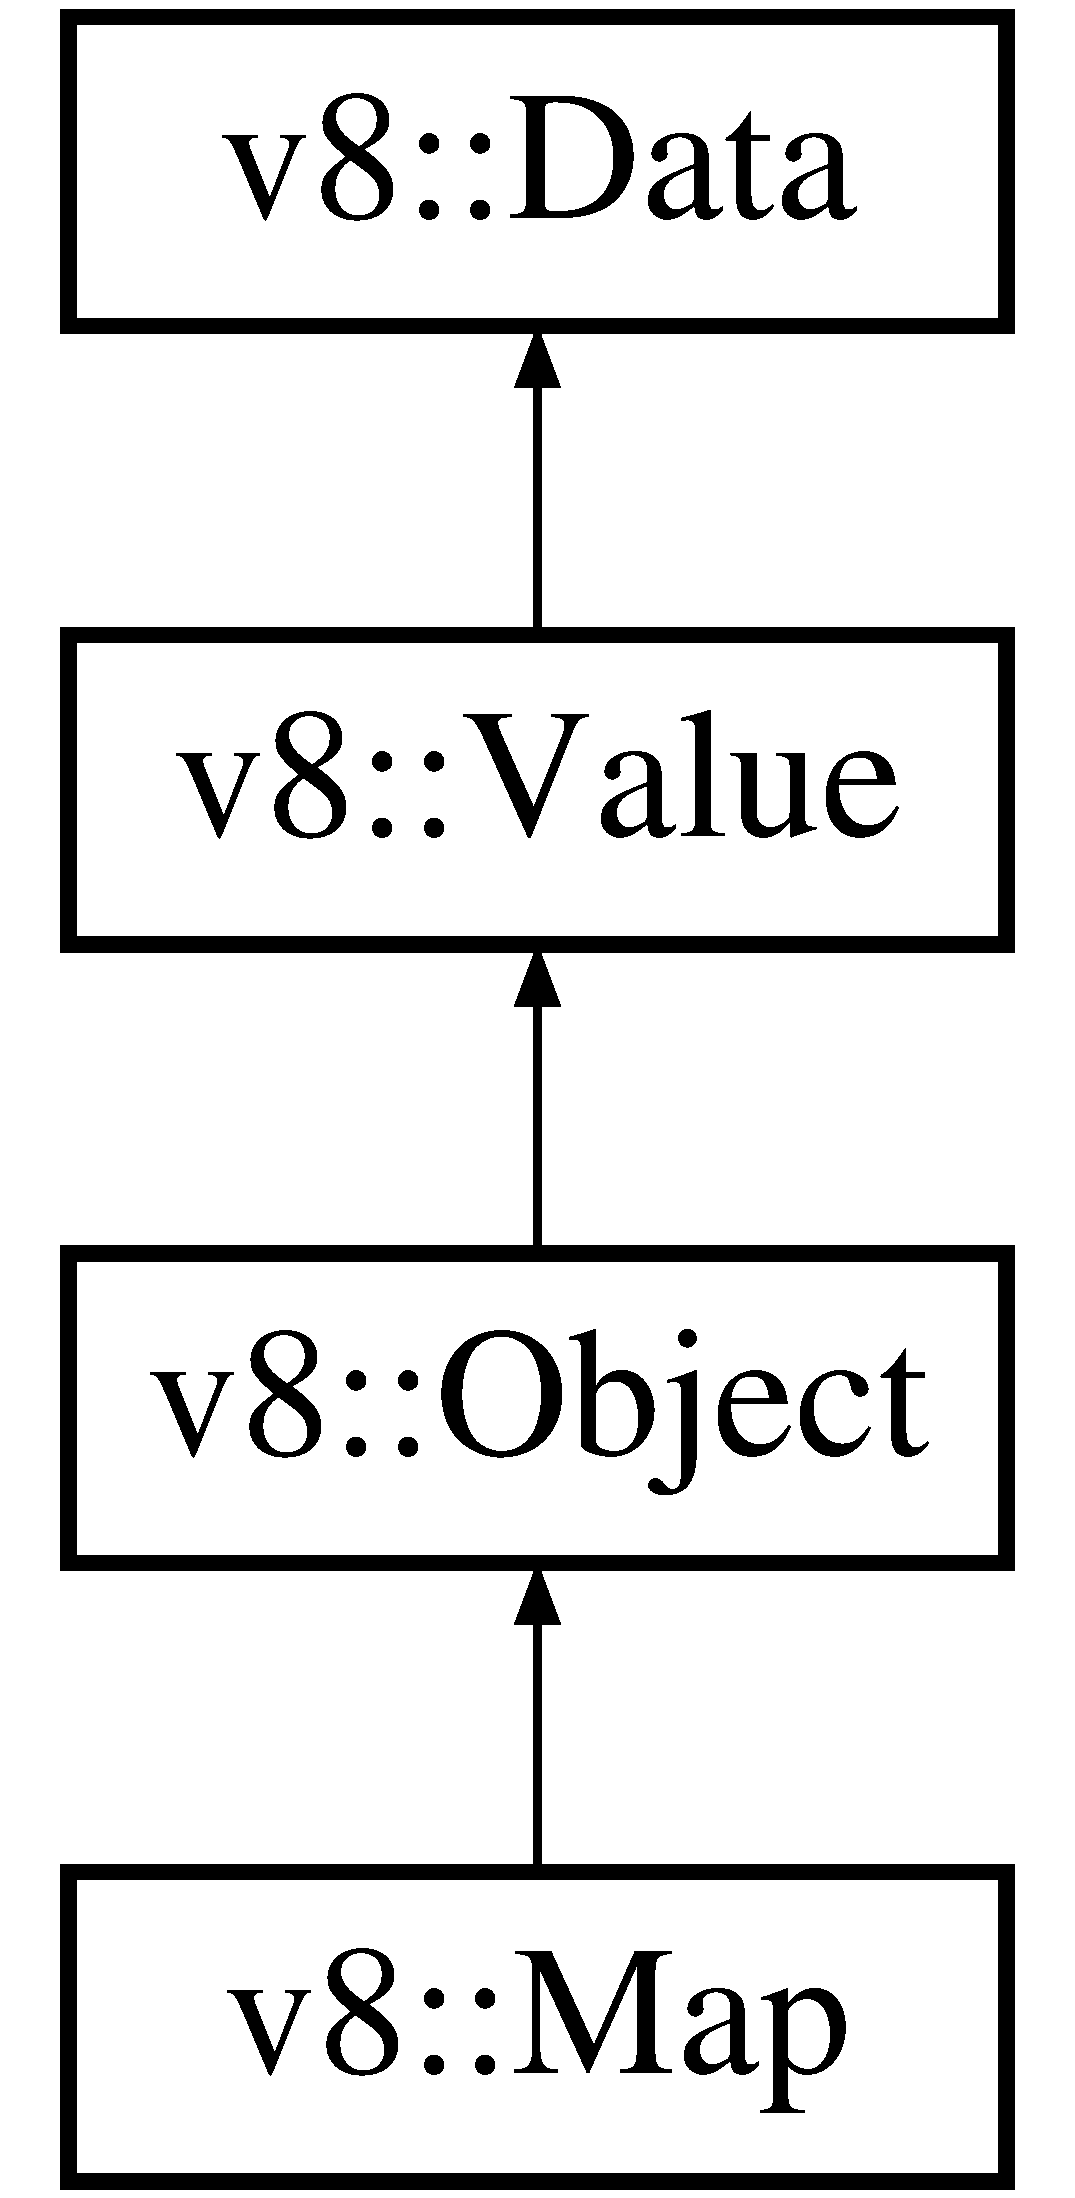
\includegraphics[height=4.000000cm]{classv8_1_1_map}
\end{center}
\end{figure}
\subsection*{Public Member Functions}
\begin{DoxyCompactItemize}
\item 
size\+\_\+t {\bfseries Size} () const \hypertarget{classv8_1_1_map_abed3aa2199c0f383a975208805d702ee}{}\label{classv8_1_1_map_abed3aa2199c0f383a975208805d702ee}

\item 
void {\bfseries Clear} ()\hypertarget{classv8_1_1_map_a06ee0d566d206058a7fe22c140000be4}{}\label{classv8_1_1_map_a06ee0d566d206058a7fe22c140000be4}

\item 
V8\+\_\+\+W\+A\+R\+N\+\_\+\+U\+N\+U\+S\+E\+D\+\_\+\+R\+E\+S\+U\+LT \hyperlink{classv8_1_1_maybe_local}{Maybe\+Local}$<$ \hyperlink{classv8_1_1_value}{Value} $>$ {\bfseries Get} (\hyperlink{classv8_1_1_local}{Local}$<$ \hyperlink{classv8_1_1_context}{Context} $>$ context, \hyperlink{classv8_1_1_local}{Local}$<$ \hyperlink{classv8_1_1_value}{Value} $>$ key)\hypertarget{classv8_1_1_map_a79c6e87f634c22b17a56252be6f3e871}{}\label{classv8_1_1_map_a79c6e87f634c22b17a56252be6f3e871}

\item 
V8\+\_\+\+W\+A\+R\+N\+\_\+\+U\+N\+U\+S\+E\+D\+\_\+\+R\+E\+S\+U\+LT \hyperlink{classv8_1_1_maybe_local}{Maybe\+Local}$<$ \hyperlink{classv8_1_1_map}{Map} $>$ {\bfseries Set} (\hyperlink{classv8_1_1_local}{Local}$<$ \hyperlink{classv8_1_1_context}{Context} $>$ context, \hyperlink{classv8_1_1_local}{Local}$<$ \hyperlink{classv8_1_1_value}{Value} $>$ key, \hyperlink{classv8_1_1_local}{Local}$<$ \hyperlink{classv8_1_1_value}{Value} $>$ value)\hypertarget{classv8_1_1_map_aac0d846409ad68783046b318fb50f764}{}\label{classv8_1_1_map_aac0d846409ad68783046b318fb50f764}

\item 
V8\+\_\+\+W\+A\+R\+N\+\_\+\+U\+N\+U\+S\+E\+D\+\_\+\+R\+E\+S\+U\+LT \hyperlink{classv8_1_1_maybe}{Maybe}$<$ bool $>$ {\bfseries Has} (\hyperlink{classv8_1_1_local}{Local}$<$ \hyperlink{classv8_1_1_context}{Context} $>$ context, \hyperlink{classv8_1_1_local}{Local}$<$ \hyperlink{classv8_1_1_value}{Value} $>$ key)\hypertarget{classv8_1_1_map_a7a4cbc33fa074d1d2b0c04a6007622c6}{}\label{classv8_1_1_map_a7a4cbc33fa074d1d2b0c04a6007622c6}

\item 
V8\+\_\+\+W\+A\+R\+N\+\_\+\+U\+N\+U\+S\+E\+D\+\_\+\+R\+E\+S\+U\+LT \hyperlink{classv8_1_1_maybe}{Maybe}$<$ bool $>$ {\bfseries Delete} (\hyperlink{classv8_1_1_local}{Local}$<$ \hyperlink{classv8_1_1_context}{Context} $>$ context, \hyperlink{classv8_1_1_local}{Local}$<$ \hyperlink{classv8_1_1_value}{Value} $>$ key)\hypertarget{classv8_1_1_map_a59d3042fd33d8fb616489a6dd8d8c53c}{}\label{classv8_1_1_map_a59d3042fd33d8fb616489a6dd8d8c53c}

\item 
\hyperlink{classv8_1_1_local}{Local}$<$ \hyperlink{classv8_1_1_array}{Array} $>$ \hyperlink{classv8_1_1_map_a6e864cea5fcb1113c5d9fdbd82cee73a}{As\+Array} () const 
\end{DoxyCompactItemize}
\subsection*{Static Public Member Functions}
\begin{DoxyCompactItemize}
\item 
static \hyperlink{classv8_1_1_local}{Local}$<$ \hyperlink{classv8_1_1_map}{Map} $>$ \hyperlink{classv8_1_1_map_a4126e8c0d6127119157986f1316380c2}{New} (\hyperlink{classv8_1_1_isolate}{Isolate} $\ast$isolate)
\item 
static V8\+\_\+\+I\+N\+L\+I\+NE \hyperlink{classv8_1_1_map}{Map} $\ast$ {\bfseries Cast} (\hyperlink{classv8_1_1_value}{Value} $\ast$obj)\hypertarget{classv8_1_1_map_ac53aafed02f275a7d3ce6da8cfd060c3}{}\label{classv8_1_1_map_ac53aafed02f275a7d3ce6da8cfd060c3}

\end{DoxyCompactItemize}
\subsection*{Static Private Member Functions}
\begin{DoxyCompactItemize}
\item 
static void {\bfseries Check\+Cast} (\hyperlink{classv8_1_1_value}{Value} $\ast$obj)\hypertarget{classv8_1_1_map_a0dc03d79213e15b9257f613c7b1d9357}{}\label{classv8_1_1_map_a0dc03d79213e15b9257f613c7b1d9357}

\end{DoxyCompactItemize}


\subsection{Detailed Description}
An instance of the built-\/in \hyperlink{classv8_1_1_map}{Map} constructor (E\+C\+M\+A-\/262, 6th Edition, 23.\+1.\+1). 

\subsection{Member Function Documentation}
\index{v8\+::\+Map@{v8\+::\+Map}!As\+Array@{As\+Array}}
\index{As\+Array@{As\+Array}!v8\+::\+Map@{v8\+::\+Map}}
\subsubsection[{\texorpdfstring{As\+Array() const }{AsArray() const }}]{\setlength{\rightskip}{0pt plus 5cm}{\bf Local}$<$ {\bf Array} $>$ v8\+::\+Map\+::\+As\+Array (
\begin{DoxyParamCaption}
{}
\end{DoxyParamCaption}
) const}\hypertarget{classv8_1_1_map_a6e864cea5fcb1113c5d9fdbd82cee73a}{}\label{classv8_1_1_map_a6e864cea5fcb1113c5d9fdbd82cee73a}
Returns an array of length Size() $\ast$ 2, where index N is the Nth key and index N + 1 is the Nth value. \index{v8\+::\+Map@{v8\+::\+Map}!New@{New}}
\index{New@{New}!v8\+::\+Map@{v8\+::\+Map}}
\subsubsection[{\texorpdfstring{New(\+Isolate $\ast$isolate)}{New(Isolate *isolate)}}]{\setlength{\rightskip}{0pt plus 5cm}{\bf Local}$<$ {\bf v8\+::\+Map} $>$ v8\+::\+Map\+::\+New (
\begin{DoxyParamCaption}
\item[{{\bf Isolate} $\ast$}]{isolate}
\end{DoxyParamCaption}
)\hspace{0.3cm}{\ttfamily [static]}}\hypertarget{classv8_1_1_map_a4126e8c0d6127119157986f1316380c2}{}\label{classv8_1_1_map_a4126e8c0d6127119157986f1316380c2}
Creates a new empty \hyperlink{classv8_1_1_map}{Map}. 

The documentation for this class was generated from the following files\+:\begin{DoxyCompactItemize}
\item 
/\+Users/joshgav/node/v8/include/v8.\+h\item 
/\+Users/joshgav/node/v8/src/api.\+cc\end{DoxyCompactItemize}

\hypertarget{classv8_1_1_maybe}{}\section{v8\+:\+:Maybe$<$ T $>$ Class Template Reference}
\label{classv8_1_1_maybe}\index{v8\+::\+Maybe$<$ T $>$@{v8\+::\+Maybe$<$ T $>$}}


{\ttfamily \#include $<$v8.\+h$>$}

\subsection*{Public Member Functions}
\begin{DoxyCompactItemize}
\item 
V8\+\_\+\+I\+N\+L\+I\+NE bool {\bfseries Is\+Nothing} () const \hypertarget{classv8_1_1_maybe_a486b608c21c8038d5019bd7d75866345}{}\label{classv8_1_1_maybe_a486b608c21c8038d5019bd7d75866345}

\item 
V8\+\_\+\+I\+N\+L\+I\+NE bool {\bfseries Is\+Just} () const \hypertarget{classv8_1_1_maybe_adc82dc945891060d312fb6fbf8fb56ae}{}\label{classv8_1_1_maybe_adc82dc945891060d312fb6fbf8fb56ae}

\item 
V8\+\_\+\+I\+N\+L\+I\+NE T {\bfseries From\+Just} () const \hypertarget{classv8_1_1_maybe_a02b19d7fcb7744d8dba3530ef8e14c8c}{}\label{classv8_1_1_maybe_a02b19d7fcb7744d8dba3530ef8e14c8c}

\item 
V8\+\_\+\+I\+N\+L\+I\+NE T {\bfseries From\+Maybe} (const T \&default\+\_\+value) const \hypertarget{classv8_1_1_maybe_a0bcb5fb0d0e92a3f0cc546f11068a8df}{}\label{classv8_1_1_maybe_a0bcb5fb0d0e92a3f0cc546f11068a8df}

\item 
V8\+\_\+\+I\+N\+L\+I\+NE bool {\bfseries operator==} (const \hyperlink{classv8_1_1_maybe}{Maybe} \&other) const \hypertarget{classv8_1_1_maybe_adf61111c2da44e10ba5ab546a9a525ce}{}\label{classv8_1_1_maybe_adf61111c2da44e10ba5ab546a9a525ce}

\item 
V8\+\_\+\+I\+N\+L\+I\+NE bool {\bfseries operator!=} (const \hyperlink{classv8_1_1_maybe}{Maybe} \&other) const \hypertarget{classv8_1_1_maybe_a5bbacc606422d7ab327c2683462342ec}{}\label{classv8_1_1_maybe_a5bbacc606422d7ab327c2683462342ec}

\end{DoxyCompactItemize}
\subsection*{Private Member Functions}
\begin{DoxyCompactItemize}
\item 
{\bfseries Maybe} (const T \&t)\hypertarget{classv8_1_1_maybe_a29ee108b5096f09e1e69b18ffc3c60cc}{}\label{classv8_1_1_maybe_a29ee108b5096f09e1e69b18ffc3c60cc}

\end{DoxyCompactItemize}
\subsection*{Private Attributes}
\begin{DoxyCompactItemize}
\item 
bool {\bfseries has\+\_\+value}\hypertarget{classv8_1_1_maybe_afd7a3ebca6d97a4b87f2829a28723b0b}{}\label{classv8_1_1_maybe_afd7a3ebca6d97a4b87f2829a28723b0b}

\item 
T {\bfseries value}\hypertarget{classv8_1_1_maybe_ac3e067a7ae1b5cc92c2f570499db31ea}{}\label{classv8_1_1_maybe_ac3e067a7ae1b5cc92c2f570499db31ea}

\end{DoxyCompactItemize}
\subsection*{Friends}
\begin{DoxyCompactItemize}
\item 
{\footnotesize template$<$class U $>$ }\\\hyperlink{classv8_1_1_maybe}{Maybe}$<$ U $>$ {\bfseries Nothing} ()\hypertarget{classv8_1_1_maybe_aeb9593e125b42d748acbd69b72c89f37}{}\label{classv8_1_1_maybe_aeb9593e125b42d748acbd69b72c89f37}

\item 
{\footnotesize template$<$class U $>$ }\\\hyperlink{classv8_1_1_maybe}{Maybe}$<$ U $>$ {\bfseries Just} (const U \&u)\hypertarget{classv8_1_1_maybe_aeff0e7fedd63cfebe9a5286e2cd8552d}{}\label{classv8_1_1_maybe_aeff0e7fedd63cfebe9a5286e2cd8552d}

\end{DoxyCompactItemize}


\subsection{Detailed Description}
\subsubsection*{template$<$class T$>$\\*
class v8\+::\+Maybe$<$ T $>$}

A simple \hyperlink{classv8_1_1_maybe}{Maybe} type, representing an object which may or may not have a value, see \href{https://hackage.haskell.org/package/base/docs/Data-Maybe.html}{\tt https\+://hackage.\+haskell.\+org/package/base/docs/\+Data-\/\+Maybe.\+html}.

If an A\+PI method returns a Maybe$<$$>$, the A\+PI method can potentially fail either because an exception is thrown, or because an exception is pending, e.\+g. because a previous A\+PI call threw an exception that hasn\textquotesingle{}t been caught yet, or because a Terminate\+Execution exception was thrown. In that case, a \char`\"{}\+Nothing\char`\"{} value is returned. 

The documentation for this class was generated from the following file\+:\begin{DoxyCompactItemize}
\item 
/\+Users/joshgav/node/v8/include/v8.\+h\end{DoxyCompactItemize}

\hypertarget{classv8_1_1_maybe_local}{}\section{v8\+:\+:Maybe\+Local$<$ T $>$ Class Template Reference}
\label{classv8_1_1_maybe_local}\index{v8\+::\+Maybe\+Local$<$ T $>$@{v8\+::\+Maybe\+Local$<$ T $>$}}


{\ttfamily \#include $<$v8.\+h$>$}

\subsection*{Public Member Functions}
\begin{DoxyCompactItemize}
\item 
{\footnotesize template$<$class S $>$ }\\V8\+\_\+\+I\+N\+L\+I\+NE {\bfseries Maybe\+Local} (\hyperlink{classv8_1_1_local}{Local}$<$ S $>$ that)\hypertarget{classv8_1_1_maybe_local_ab488843c2faf4375517616d3c66886e5}{}\label{classv8_1_1_maybe_local_ab488843c2faf4375517616d3c66886e5}

\item 
V8\+\_\+\+I\+N\+L\+I\+NE bool {\bfseries Is\+Empty} () const \hypertarget{classv8_1_1_maybe_local_a6d1f2acdc91800c481977d86ae04aa53}{}\label{classv8_1_1_maybe_local_a6d1f2acdc91800c481977d86ae04aa53}

\item 
{\footnotesize template$<$class S $>$ }\\V8\+\_\+\+W\+A\+R\+N\+\_\+\+U\+N\+U\+S\+E\+D\+\_\+\+R\+E\+S\+U\+LT V8\+\_\+\+I\+N\+L\+I\+NE bool {\bfseries To\+Local} (\hyperlink{classv8_1_1_local}{Local}$<$ S $>$ $\ast$out) const \hypertarget{classv8_1_1_maybe_local_af3e66ed0bbc8845081fba2488c507c6a}{}\label{classv8_1_1_maybe_local_af3e66ed0bbc8845081fba2488c507c6a}

\item 
V8\+\_\+\+I\+N\+L\+I\+NE \hyperlink{classv8_1_1_local}{Local}$<$ T $>$ {\bfseries To\+Local\+Checked} ()\hypertarget{classv8_1_1_maybe_local_a9b2c9d50fca5897e3a03fd4c25d12415}{}\label{classv8_1_1_maybe_local_a9b2c9d50fca5897e3a03fd4c25d12415}

\item 
{\footnotesize template$<$class S $>$ }\\V8\+\_\+\+I\+N\+L\+I\+NE \hyperlink{classv8_1_1_local}{Local}$<$ S $>$ {\bfseries From\+Maybe} (\hyperlink{classv8_1_1_local}{Local}$<$ S $>$ default\+\_\+value) const \hypertarget{classv8_1_1_maybe_local_afe1aea162c64385160cc1c83df859eaf}{}\label{classv8_1_1_maybe_local_afe1aea162c64385160cc1c83df859eaf}

\end{DoxyCompactItemize}
\subsection*{Private Attributes}
\begin{DoxyCompactItemize}
\item 
T $\ast$ {\bfseries val\+\_\+}\hypertarget{classv8_1_1_maybe_local_aaaa3e33a607bc6d243fe00875a345cc5}{}\label{classv8_1_1_maybe_local_aaaa3e33a607bc6d243fe00875a345cc5}

\end{DoxyCompactItemize}


\subsection{Detailed Description}
\subsubsection*{template$<$class T$>$\\*
class v8\+::\+Maybe\+Local$<$ T $>$}

A Maybe\+Local$<$$>$ is a wrapper around Local$<$$>$ that enforces a check whether the Local$<$$>$ is empty before it can be used.

If an A\+PI method returns a Maybe\+Local$<$$>$, the A\+PI method can potentially fail either because an exception is thrown, or because an exception is pending, e.\+g. because a previous A\+PI call threw an exception that hasn\textquotesingle{}t been caught yet, or because a Terminate\+Execution exception was thrown. In that case, an empty \hyperlink{classv8_1_1_maybe_local}{Maybe\+Local} is returned. 

The documentation for this class was generated from the following file\+:\begin{DoxyCompactItemize}
\item 
include/v8.\+h\end{DoxyCompactItemize}

\hypertarget{classv8_1_1_message}{}\section{v8\+:\+:Message Class Reference}
\label{classv8_1_1_message}\index{v8\+::\+Message@{v8\+::\+Message}}


{\ttfamily \#include $<$v8.\+h$>$}

\subsection*{Public Member Functions}
\begin{DoxyCompactItemize}
\item 
\hyperlink{classv8_1_1_local}{Local}$<$ \hyperlink{classv8_1_1_string}{String} $>$ {\bfseries Get} () const \hypertarget{classv8_1_1_message_a72f26c7b684bbfbd14d5970849fdf3d2}{}\label{classv8_1_1_message_a72f26c7b684bbfbd14d5970849fdf3d2}

\item 
{\bfseries V8\+\_\+\+D\+E\+P\+R\+E\+C\+A\+T\+E\+\_\+\+S\+O\+ON} (\char`\"{}Use maybe version\char`\"{}, Local$<$ \hyperlink{classv8_1_1_string}{String} $>$ Get\+Source\+Line() const)\hypertarget{classv8_1_1_message_abcb8b2005ba077d855c4fcf775151fd6}{}\label{classv8_1_1_message_abcb8b2005ba077d855c4fcf775151fd6}

\item 
V8\+\_\+\+W\+A\+R\+N\+\_\+\+U\+N\+U\+S\+E\+D\+\_\+\+R\+E\+S\+U\+LT \hyperlink{classv8_1_1_maybe_local}{Maybe\+Local}$<$ \hyperlink{classv8_1_1_string}{String} $>$ {\bfseries Get\+Source\+Line} (\hyperlink{classv8_1_1_local}{Local}$<$ \hyperlink{classv8_1_1_context}{Context} $>$ context) const \hypertarget{classv8_1_1_message_a036059b3f15a98f9814f470b65948956}{}\label{classv8_1_1_message_a036059b3f15a98f9814f470b65948956}

\item 
\hyperlink{classv8_1_1_script_origin}{Script\+Origin} \hyperlink{classv8_1_1_message_ae0fc442f44bd2b600c4d89a50cf3abd9}{Get\+Script\+Origin} () const 
\item 
\hyperlink{classv8_1_1_local}{Local}$<$ \hyperlink{classv8_1_1_value}{Value} $>$ \hyperlink{classv8_1_1_message_a66200e721dc4aa00568099ba67e9143a}{Get\+Script\+Resource\+Name} () const 
\item 
\hyperlink{classv8_1_1_local}{Local}$<$ \hyperlink{classv8_1_1_stack_trace}{Stack\+Trace} $>$ \hyperlink{classv8_1_1_message_a42738680a1f28c495010a76b73373445}{Get\+Stack\+Trace} () const 
\item 
\hyperlink{classv8_1_1_message_a0a6855ef9eda008aa0f06f8cdf2a41e4}{V8\+\_\+\+D\+E\+P\+R\+E\+C\+A\+T\+E\+\_\+\+S\+O\+ON} (\char`\"{}Use maybe version\char`\"{}, int Get\+Line\+Number() const)
\item 
V8\+\_\+\+W\+A\+R\+N\+\_\+\+U\+N\+U\+S\+E\+D\+\_\+\+R\+E\+S\+U\+LT \hyperlink{classv8_1_1_maybe}{Maybe}$<$ int $>$ {\bfseries Get\+Line\+Number} (\hyperlink{classv8_1_1_local}{Local}$<$ \hyperlink{classv8_1_1_context}{Context} $>$ context) const \hypertarget{classv8_1_1_message_a9425c8d1b3f7e3a066458c676642c6df}{}\label{classv8_1_1_message_a9425c8d1b3f7e3a066458c676642c6df}

\item 
int \hyperlink{classv8_1_1_message_a31a550a1d3d09a2d72d0742be821956f}{Get\+Start\+Position} () const 
\item 
int \hyperlink{classv8_1_1_message_a50cbec87379e628b1647466926882037}{Get\+End\+Position} () const 
\item 
\hyperlink{classv8_1_1_message_a4715c868bd87bbc65a74c8aca27ec692}{V8\+\_\+\+D\+E\+P\+R\+E\+C\+A\+T\+E\+\_\+\+S\+O\+ON} (\char`\"{}Use maybe version\char`\"{}, int Get\+Start\+Column() const)
\item 
V8\+\_\+\+W\+A\+R\+N\+\_\+\+U\+N\+U\+S\+E\+D\+\_\+\+R\+E\+S\+U\+LT \hyperlink{classv8_1_1_maybe}{Maybe}$<$ int $>$ {\bfseries Get\+Start\+Column} (\hyperlink{classv8_1_1_local}{Local}$<$ \hyperlink{classv8_1_1_context}{Context} $>$ context) const \hypertarget{classv8_1_1_message_aedffb63ec9761af77b9492351b0bd8a2}{}\label{classv8_1_1_message_aedffb63ec9761af77b9492351b0bd8a2}

\item 
\hyperlink{classv8_1_1_message_a411046bd092195ddc21525c0e68ee424}{V8\+\_\+\+D\+E\+P\+R\+E\+C\+A\+T\+ED} (\char`\"{}Use maybe version\char`\"{}, int Get\+End\+Column() const)
\item 
V8\+\_\+\+W\+A\+R\+N\+\_\+\+U\+N\+U\+S\+E\+D\+\_\+\+R\+E\+S\+U\+LT \hyperlink{classv8_1_1_maybe}{Maybe}$<$ int $>$ {\bfseries Get\+End\+Column} (\hyperlink{classv8_1_1_local}{Local}$<$ \hyperlink{classv8_1_1_context}{Context} $>$ context) const \hypertarget{classv8_1_1_message_aa6f918e778dd9ad173dbdfa75c9f614f}{}\label{classv8_1_1_message_aa6f918e778dd9ad173dbdfa75c9f614f}

\item 
bool \hyperlink{classv8_1_1_message_a03228f50c40c45da52f424bdd64598d1}{Is\+Shared\+Cross\+Origin} () const 
\item 
bool {\bfseries Is\+Opaque} () const \hypertarget{classv8_1_1_message_a2ab104d29e13bc942f345e09472ed531}{}\label{classv8_1_1_message_a2ab104d29e13bc942f345e09472ed531}

\end{DoxyCompactItemize}
\subsection*{Static Public Member Functions}
\begin{DoxyCompactItemize}
\item 
static void {\bfseries Print\+Current\+Stack\+Trace} (\hyperlink{classv8_1_1_isolate}{Isolate} $\ast$isolate, F\+I\+LE $\ast$out)\hypertarget{classv8_1_1_message_ae5d67d123c5611e6bc36824c938cbfa5}{}\label{classv8_1_1_message_ae5d67d123c5611e6bc36824c938cbfa5}

\end{DoxyCompactItemize}
\subsection*{Static Public Attributes}
\begin{DoxyCompactItemize}
\item 
static const int {\bfseries k\+No\+Line\+Number\+Info} = 0\hypertarget{classv8_1_1_message_a35649a6c0c813ba82c9886a2b17da124}{}\label{classv8_1_1_message_a35649a6c0c813ba82c9886a2b17da124}

\item 
static const int {\bfseries k\+No\+Column\+Info} = 0\hypertarget{classv8_1_1_message_a8cb643dbf408b0fd2526b23a8202c4a6}{}\label{classv8_1_1_message_a8cb643dbf408b0fd2526b23a8202c4a6}

\item 
static const int {\bfseries k\+No\+Script\+Id\+Info} = 0\hypertarget{classv8_1_1_message_a5aac643173466e88544cb1daa74553d6}{}\label{classv8_1_1_message_a5aac643173466e88544cb1daa74553d6}

\end{DoxyCompactItemize}


\subsection{Detailed Description}
An error message. 

\subsection{Member Function Documentation}
\index{v8\+::\+Message@{v8\+::\+Message}!Get\+End\+Position@{Get\+End\+Position}}
\index{Get\+End\+Position@{Get\+End\+Position}!v8\+::\+Message@{v8\+::\+Message}}
\subsubsection[{\texorpdfstring{Get\+End\+Position() const }{GetEndPosition() const }}]{\setlength{\rightskip}{0pt plus 5cm}int v8\+::\+Message\+::\+Get\+End\+Position (
\begin{DoxyParamCaption}
{}
\end{DoxyParamCaption}
) const}\hypertarget{classv8_1_1_message_a50cbec87379e628b1647466926882037}{}\label{classv8_1_1_message_a50cbec87379e628b1647466926882037}
Returns the index within the script of the last character where the error occurred. \index{v8\+::\+Message@{v8\+::\+Message}!Get\+Script\+Origin@{Get\+Script\+Origin}}
\index{Get\+Script\+Origin@{Get\+Script\+Origin}!v8\+::\+Message@{v8\+::\+Message}}
\subsubsection[{\texorpdfstring{Get\+Script\+Origin() const }{GetScriptOrigin() const }}]{\setlength{\rightskip}{0pt plus 5cm}{\bf Script\+Origin} v8\+::\+Message\+::\+Get\+Script\+Origin (
\begin{DoxyParamCaption}
{}
\end{DoxyParamCaption}
) const}\hypertarget{classv8_1_1_message_ae0fc442f44bd2b600c4d89a50cf3abd9}{}\label{classv8_1_1_message_ae0fc442f44bd2b600c4d89a50cf3abd9}
Returns the origin for the script from where the function causing the error originates. \index{v8\+::\+Message@{v8\+::\+Message}!Get\+Script\+Resource\+Name@{Get\+Script\+Resource\+Name}}
\index{Get\+Script\+Resource\+Name@{Get\+Script\+Resource\+Name}!v8\+::\+Message@{v8\+::\+Message}}
\subsubsection[{\texorpdfstring{Get\+Script\+Resource\+Name() const }{GetScriptResourceName() const }}]{\setlength{\rightskip}{0pt plus 5cm}{\bf Local}$<${\bf Value}$>$ v8\+::\+Message\+::\+Get\+Script\+Resource\+Name (
\begin{DoxyParamCaption}
{}
\end{DoxyParamCaption}
) const}\hypertarget{classv8_1_1_message_a66200e721dc4aa00568099ba67e9143a}{}\label{classv8_1_1_message_a66200e721dc4aa00568099ba67e9143a}
Returns the resource name for the script from where the function causing the error originates. \index{v8\+::\+Message@{v8\+::\+Message}!Get\+Stack\+Trace@{Get\+Stack\+Trace}}
\index{Get\+Stack\+Trace@{Get\+Stack\+Trace}!v8\+::\+Message@{v8\+::\+Message}}
\subsubsection[{\texorpdfstring{Get\+Stack\+Trace() const }{GetStackTrace() const }}]{\setlength{\rightskip}{0pt plus 5cm}{\bf Local}$<${\bf Stack\+Trace}$>$ v8\+::\+Message\+::\+Get\+Stack\+Trace (
\begin{DoxyParamCaption}
{}
\end{DoxyParamCaption}
) const}\hypertarget{classv8_1_1_message_a42738680a1f28c495010a76b73373445}{}\label{classv8_1_1_message_a42738680a1f28c495010a76b73373445}
\hyperlink{classv8_1_1_exception}{Exception} stack trace. By default stack traces are not captured for uncaught exceptions. Set\+Capture\+Stack\+Trace\+For\+Uncaught\+Exceptions allows to change this option. \index{v8\+::\+Message@{v8\+::\+Message}!Get\+Start\+Position@{Get\+Start\+Position}}
\index{Get\+Start\+Position@{Get\+Start\+Position}!v8\+::\+Message@{v8\+::\+Message}}
\subsubsection[{\texorpdfstring{Get\+Start\+Position() const }{GetStartPosition() const }}]{\setlength{\rightskip}{0pt plus 5cm}int v8\+::\+Message\+::\+Get\+Start\+Position (
\begin{DoxyParamCaption}
{}
\end{DoxyParamCaption}
) const}\hypertarget{classv8_1_1_message_a31a550a1d3d09a2d72d0742be821956f}{}\label{classv8_1_1_message_a31a550a1d3d09a2d72d0742be821956f}
Returns the index within the script of the first character where the error occurred. \index{v8\+::\+Message@{v8\+::\+Message}!Is\+Shared\+Cross\+Origin@{Is\+Shared\+Cross\+Origin}}
\index{Is\+Shared\+Cross\+Origin@{Is\+Shared\+Cross\+Origin}!v8\+::\+Message@{v8\+::\+Message}}
\subsubsection[{\texorpdfstring{Is\+Shared\+Cross\+Origin() const }{IsSharedCrossOrigin() const }}]{\setlength{\rightskip}{0pt plus 5cm}bool v8\+::\+Message\+::\+Is\+Shared\+Cross\+Origin (
\begin{DoxyParamCaption}
{}
\end{DoxyParamCaption}
) const}\hypertarget{classv8_1_1_message_a03228f50c40c45da52f424bdd64598d1}{}\label{classv8_1_1_message_a03228f50c40c45da52f424bdd64598d1}
Passes on the value set by the embedder when it fed the script from which this \hyperlink{classv8_1_1_message}{Message} was generated to \hyperlink{classv8_1_1_v8}{V8}. \index{v8\+::\+Message@{v8\+::\+Message}!V8\+\_\+\+D\+E\+P\+R\+E\+C\+A\+T\+E\+\_\+\+S\+O\+ON@{V8\+\_\+\+D\+E\+P\+R\+E\+C\+A\+T\+E\+\_\+\+S\+O\+ON}}
\index{V8\+\_\+\+D\+E\+P\+R\+E\+C\+A\+T\+E\+\_\+\+S\+O\+ON@{V8\+\_\+\+D\+E\+P\+R\+E\+C\+A\+T\+E\+\_\+\+S\+O\+ON}!v8\+::\+Message@{v8\+::\+Message}}
\subsubsection[{\texorpdfstring{V8\+\_\+\+D\+E\+P\+R\+E\+C\+A\+T\+E\+\_\+\+S\+O\+O\+N(""Use maybe version"", int Get\+Line\+Number() const)}{V8_DEPRECATE_SOON("Use maybe version", int GetLineNumber() const)}}]{\setlength{\rightskip}{0pt plus 5cm}v8\+::\+Message\+::\+V8\+\_\+\+D\+E\+P\+R\+E\+C\+A\+T\+E\+\_\+\+S\+O\+ON (
\begin{DoxyParamCaption}
\item[{\char`\"{}Use maybe version\char`\"{}}]{, }
\item[{int Get\+Line\+Number()}]{const}
\end{DoxyParamCaption}
)}\hypertarget{classv8_1_1_message_a0a6855ef9eda008aa0f06f8cdf2a41e4}{}\label{classv8_1_1_message_a0a6855ef9eda008aa0f06f8cdf2a41e4}
Returns the number, 1-\/based, of the line where the error occurred. \index{v8\+::\+Message@{v8\+::\+Message}!V8\+\_\+\+D\+E\+P\+R\+E\+C\+A\+T\+E\+\_\+\+S\+O\+ON@{V8\+\_\+\+D\+E\+P\+R\+E\+C\+A\+T\+E\+\_\+\+S\+O\+ON}}
\index{V8\+\_\+\+D\+E\+P\+R\+E\+C\+A\+T\+E\+\_\+\+S\+O\+ON@{V8\+\_\+\+D\+E\+P\+R\+E\+C\+A\+T\+E\+\_\+\+S\+O\+ON}!v8\+::\+Message@{v8\+::\+Message}}
\subsubsection[{\texorpdfstring{V8\+\_\+\+D\+E\+P\+R\+E\+C\+A\+T\+E\+\_\+\+S\+O\+O\+N(""Use maybe version"", int Get\+Start\+Column() const)}{V8_DEPRECATE_SOON("Use maybe version", int GetStartColumn() const)}}]{\setlength{\rightskip}{0pt plus 5cm}v8\+::\+Message\+::\+V8\+\_\+\+D\+E\+P\+R\+E\+C\+A\+T\+E\+\_\+\+S\+O\+ON (
\begin{DoxyParamCaption}
\item[{\char`\"{}Use maybe version\char`\"{}}]{, }
\item[{int Get\+Start\+Column()}]{const}
\end{DoxyParamCaption}
)}\hypertarget{classv8_1_1_message_a4715c868bd87bbc65a74c8aca27ec692}{}\label{classv8_1_1_message_a4715c868bd87bbc65a74c8aca27ec692}
Returns the index within the line of the first character where the error occurred. \index{v8\+::\+Message@{v8\+::\+Message}!V8\+\_\+\+D\+E\+P\+R\+E\+C\+A\+T\+ED@{V8\+\_\+\+D\+E\+P\+R\+E\+C\+A\+T\+ED}}
\index{V8\+\_\+\+D\+E\+P\+R\+E\+C\+A\+T\+ED@{V8\+\_\+\+D\+E\+P\+R\+E\+C\+A\+T\+ED}!v8\+::\+Message@{v8\+::\+Message}}
\subsubsection[{\texorpdfstring{V8\+\_\+\+D\+E\+P\+R\+E\+C\+A\+T\+E\+D(""Use maybe version"", int Get\+End\+Column() const)}{V8_DEPRECATED("Use maybe version", int GetEndColumn() const)}}]{\setlength{\rightskip}{0pt plus 5cm}v8\+::\+Message\+::\+V8\+\_\+\+D\+E\+P\+R\+E\+C\+A\+T\+ED (
\begin{DoxyParamCaption}
\item[{\char`\"{}Use maybe version\char`\"{}}]{, }
\item[{int Get\+End\+Column()}]{const}
\end{DoxyParamCaption}
)}\hypertarget{classv8_1_1_message_a411046bd092195ddc21525c0e68ee424}{}\label{classv8_1_1_message_a411046bd092195ddc21525c0e68ee424}
Returns the index within the line of the last character where the error occurred. 

The documentation for this class was generated from the following file\+:\begin{DoxyCompactItemize}
\item 
/\+Users/joshgav/node/v8/include/v8.\+h\end{DoxyCompactItemize}

\hypertarget{classv8_1_1_debug_1_1_message}{}\section{v8\+:\+:Debug\+:\+:Message Class Reference}
\label{classv8_1_1_debug_1_1_message}\index{v8\+::\+Debug\+::\+Message@{v8\+::\+Debug\+::\+Message}}


{\ttfamily \#include $<$v8-\/debug.\+h$>$}

\subsection*{Public Member Functions}
\begin{DoxyCompactItemize}
\item 
virtual bool \hyperlink{classv8_1_1_debug_1_1_message_a371afb8f4b2352ea15ee8c7daa7f788e}{Is\+Event} () const  =0
\item 
virtual bool {\bfseries Is\+Response} () const  =0\hypertarget{classv8_1_1_debug_1_1_message_a2f6fecc2b94673088b2909a9455dc836}{}\label{classv8_1_1_debug_1_1_message_a2f6fecc2b94673088b2909a9455dc836}

\item 
virtual Debug\+Event {\bfseries Get\+Event} () const  =0\hypertarget{classv8_1_1_debug_1_1_message_a52b16e72cacf798ba633b4afc6eccf53}{}\label{classv8_1_1_debug_1_1_message_a52b16e72cacf798ba633b4afc6eccf53}

\item 
virtual bool \hyperlink{classv8_1_1_debug_1_1_message_ae6197bbed731299fd7d49d072c5ea53a}{Will\+Start\+Running} () const  =0
\item 
virtual \hyperlink{classv8_1_1_local}{Local}$<$ \hyperlink{classv8_1_1_object}{Object} $>$ \hyperlink{classv8_1_1_debug_1_1_message_a2c7a09ecad899d9ce253399776d64e91}{Get\+Execution\+State} () const  =0
\item 
virtual \hyperlink{classv8_1_1_local}{Local}$<$ \hyperlink{classv8_1_1_object}{Object} $>$ {\bfseries Get\+Event\+Data} () const  =0\hypertarget{classv8_1_1_debug_1_1_message_a0b1b18243e91c4a525e1776e79faeb8b}{}\label{classv8_1_1_debug_1_1_message_a0b1b18243e91c4a525e1776e79faeb8b}

\item 
virtual \hyperlink{classv8_1_1_local}{Local}$<$ \hyperlink{classv8_1_1_string}{String} $>$ \hyperlink{classv8_1_1_debug_1_1_message_aa5e2fc7a5a529683bb4dc176fb788cd2}{Get\+J\+S\+ON} () const  =0
\item 
virtual \hyperlink{classv8_1_1_local}{Local}$<$ \hyperlink{classv8_1_1_context}{Context} $>$ \hyperlink{classv8_1_1_debug_1_1_message_aee14299740566b578b75a89bf485cc77}{Get\+Event\+Context} () const  =0
\item 
virtual \hyperlink{classv8_1_1_debug_1_1_client_data}{Client\+Data} $\ast$ \hyperlink{classv8_1_1_debug_1_1_message_a03ec05ff968a01bbe8bb59ac82516bce}{Get\+Client\+Data} () const  =0
\item 
virtual \hyperlink{classv8_1_1_isolate}{Isolate} $\ast$ {\bfseries Get\+Isolate} () const  =0\hypertarget{classv8_1_1_debug_1_1_message_ac19f1b6a8944959c3c5e08567e77f61d}{}\label{classv8_1_1_debug_1_1_message_ac19f1b6a8944959c3c5e08567e77f61d}

\end{DoxyCompactItemize}


\subsection{Detailed Description}
A message object passed to the debug message handler. 

\subsection{Member Function Documentation}
\index{v8\+::\+Debug\+::\+Message@{v8\+::\+Debug\+::\+Message}!Get\+Client\+Data@{Get\+Client\+Data}}
\index{Get\+Client\+Data@{Get\+Client\+Data}!v8\+::\+Debug\+::\+Message@{v8\+::\+Debug\+::\+Message}}
\subsubsection[{\texorpdfstring{Get\+Client\+Data() const  =0}{GetClientData() const  =0}}]{\setlength{\rightskip}{0pt plus 5cm}virtual {\bf Client\+Data}$\ast$ v8\+::\+Debug\+::\+Message\+::\+Get\+Client\+Data (
\begin{DoxyParamCaption}
{}
\end{DoxyParamCaption}
) const\hspace{0.3cm}{\ttfamily [pure virtual]}}\hypertarget{classv8_1_1_debug_1_1_message_a03ec05ff968a01bbe8bb59ac82516bce}{}\label{classv8_1_1_debug_1_1_message_a03ec05ff968a01bbe8bb59ac82516bce}
Client data passed with the corresponding request if any. This is the client\+\_\+data data value passed into Debug\+::\+Send\+Command along with the request that led to the message or N\+U\+LL if the message is an event. The debugger takes ownership of the data and will delete it even if there is no message handler. \index{v8\+::\+Debug\+::\+Message@{v8\+::\+Debug\+::\+Message}!Get\+Event\+Context@{Get\+Event\+Context}}
\index{Get\+Event\+Context@{Get\+Event\+Context}!v8\+::\+Debug\+::\+Message@{v8\+::\+Debug\+::\+Message}}
\subsubsection[{\texorpdfstring{Get\+Event\+Context() const  =0}{GetEventContext() const  =0}}]{\setlength{\rightskip}{0pt plus 5cm}virtual {\bf Local}$<${\bf Context}$>$ v8\+::\+Debug\+::\+Message\+::\+Get\+Event\+Context (
\begin{DoxyParamCaption}
{}
\end{DoxyParamCaption}
) const\hspace{0.3cm}{\ttfamily [pure virtual]}}\hypertarget{classv8_1_1_debug_1_1_message_aee14299740566b578b75a89bf485cc77}{}\label{classv8_1_1_debug_1_1_message_aee14299740566b578b75a89bf485cc77}
Get the context active when the debug event happened. Note this is not the current active context as the Java\+Script part of the debugger is running in its own context which is entered at this point. \index{v8\+::\+Debug\+::\+Message@{v8\+::\+Debug\+::\+Message}!Get\+Execution\+State@{Get\+Execution\+State}}
\index{Get\+Execution\+State@{Get\+Execution\+State}!v8\+::\+Debug\+::\+Message@{v8\+::\+Debug\+::\+Message}}
\subsubsection[{\texorpdfstring{Get\+Execution\+State() const  =0}{GetExecutionState() const  =0}}]{\setlength{\rightskip}{0pt plus 5cm}virtual {\bf Local}$<${\bf Object}$>$ v8\+::\+Debug\+::\+Message\+::\+Get\+Execution\+State (
\begin{DoxyParamCaption}
{}
\end{DoxyParamCaption}
) const\hspace{0.3cm}{\ttfamily [pure virtual]}}\hypertarget{classv8_1_1_debug_1_1_message_a2c7a09ecad899d9ce253399776d64e91}{}\label{classv8_1_1_debug_1_1_message_a2c7a09ecad899d9ce253399776d64e91}
Access to execution state and event data. Don\textquotesingle{}t store these cross callbacks as their content becomes invalid. These objects are from the debugger event that started the debug message loop. \index{v8\+::\+Debug\+::\+Message@{v8\+::\+Debug\+::\+Message}!Get\+J\+S\+ON@{Get\+J\+S\+ON}}
\index{Get\+J\+S\+ON@{Get\+J\+S\+ON}!v8\+::\+Debug\+::\+Message@{v8\+::\+Debug\+::\+Message}}
\subsubsection[{\texorpdfstring{Get\+J\+S\+O\+N() const  =0}{GetJSON() const  =0}}]{\setlength{\rightskip}{0pt plus 5cm}virtual {\bf Local}$<${\bf String}$>$ v8\+::\+Debug\+::\+Message\+::\+Get\+J\+S\+ON (
\begin{DoxyParamCaption}
{}
\end{DoxyParamCaption}
) const\hspace{0.3cm}{\ttfamily [pure virtual]}}\hypertarget{classv8_1_1_debug_1_1_message_aa5e2fc7a5a529683bb4dc176fb788cd2}{}\label{classv8_1_1_debug_1_1_message_aa5e2fc7a5a529683bb4dc176fb788cd2}
Get the debugger protocol \hyperlink{classv8_1_1_j_s_o_n}{J\+S\+ON}. \index{v8\+::\+Debug\+::\+Message@{v8\+::\+Debug\+::\+Message}!Is\+Event@{Is\+Event}}
\index{Is\+Event@{Is\+Event}!v8\+::\+Debug\+::\+Message@{v8\+::\+Debug\+::\+Message}}
\subsubsection[{\texorpdfstring{Is\+Event() const  =0}{IsEvent() const  =0}}]{\setlength{\rightskip}{0pt plus 5cm}virtual bool v8\+::\+Debug\+::\+Message\+::\+Is\+Event (
\begin{DoxyParamCaption}
{}
\end{DoxyParamCaption}
) const\hspace{0.3cm}{\ttfamily [pure virtual]}}\hypertarget{classv8_1_1_debug_1_1_message_a371afb8f4b2352ea15ee8c7daa7f788e}{}\label{classv8_1_1_debug_1_1_message_a371afb8f4b2352ea15ee8c7daa7f788e}
Check type of message. \index{v8\+::\+Debug\+::\+Message@{v8\+::\+Debug\+::\+Message}!Will\+Start\+Running@{Will\+Start\+Running}}
\index{Will\+Start\+Running@{Will\+Start\+Running}!v8\+::\+Debug\+::\+Message@{v8\+::\+Debug\+::\+Message}}
\subsubsection[{\texorpdfstring{Will\+Start\+Running() const  =0}{WillStartRunning() const  =0}}]{\setlength{\rightskip}{0pt plus 5cm}virtual bool v8\+::\+Debug\+::\+Message\+::\+Will\+Start\+Running (
\begin{DoxyParamCaption}
{}
\end{DoxyParamCaption}
) const\hspace{0.3cm}{\ttfamily [pure virtual]}}\hypertarget{classv8_1_1_debug_1_1_message_ae6197bbed731299fd7d49d072c5ea53a}{}\label{classv8_1_1_debug_1_1_message_ae6197bbed731299fd7d49d072c5ea53a}
Indicate whether this is a response to a continue command which will start the VM running after this is processed. 

The documentation for this class was generated from the following file\+:\begin{DoxyCompactItemize}
\item 
/\+Users/joshgav/node/v8/include/v8-\/debug.\+h\end{DoxyCompactItemize}

\hypertarget{classv8_1_1_microtasks_scope}{}\section{v8\+:\+:Microtasks\+Scope Class Reference}
\label{classv8_1_1_microtasks_scope}\index{v8\+::\+Microtasks\+Scope@{v8\+::\+Microtasks\+Scope}}


{\ttfamily \#include $<$v8.\+h$>$}

\subsection*{Public Types}
\begin{DoxyCompactItemize}
\item 
enum {\bfseries Type} \{ \\*
{\bfseries k\+Run\+Microtasks}, 
\\*
{\bfseries k\+Do\+Not\+Run\+Microtasks}
 \}\hypertarget{classv8_1_1_microtasks_scope_a826cf210978221741a0467cd9be6996f}{}\label{classv8_1_1_microtasks_scope_a826cf210978221741a0467cd9be6996f}

\end{DoxyCompactItemize}
\subsection*{Public Member Functions}
\begin{DoxyCompactItemize}
\item 
{\bfseries Microtasks\+Scope} (\hyperlink{classv8_1_1_isolate}{Isolate} $\ast$isolate, Type type)\hypertarget{classv8_1_1_microtasks_scope_a40348ac94c7e9ea405c2546d94d9d927}{}\label{classv8_1_1_microtasks_scope_a40348ac94c7e9ea405c2546d94d9d927}

\end{DoxyCompactItemize}
\subsection*{Static Public Member Functions}
\begin{DoxyCompactItemize}
\item 
static void \hyperlink{classv8_1_1_microtasks_scope_a7c181251fc02bd2b5a1051e5de8fe4ed}{Perform\+Checkpoint} (\hyperlink{classv8_1_1_isolate}{Isolate} $\ast$isolate)
\item 
static int \hyperlink{classv8_1_1_microtasks_scope_a4ae6e290dff532252ebbca9c11829dbd}{Get\+Current\+Depth} (\hyperlink{classv8_1_1_isolate}{Isolate} $\ast$isolate)
\item 
static bool \hyperlink{classv8_1_1_microtasks_scope_a0a07be94ea87994bcfa79c9e6eb73164}{Is\+Running\+Microtasks} (\hyperlink{classv8_1_1_isolate}{Isolate} $\ast$isolate)
\end{DoxyCompactItemize}
\subsection*{Private Member Functions}
\begin{DoxyCompactItemize}
\item 
{\bfseries Microtasks\+Scope} (const \hyperlink{classv8_1_1_microtasks_scope}{Microtasks\+Scope} \&)\hypertarget{classv8_1_1_microtasks_scope_a393a4ab5a2737ca8dc64d37bfffbc50b}{}\label{classv8_1_1_microtasks_scope_a393a4ab5a2737ca8dc64d37bfffbc50b}

\item 
\hyperlink{classv8_1_1_microtasks_scope}{Microtasks\+Scope} \& {\bfseries operator=} (const \hyperlink{classv8_1_1_microtasks_scope}{Microtasks\+Scope} \&)\hypertarget{classv8_1_1_microtasks_scope_aa50f4629682aa6ae194f230e1f6f7743}{}\label{classv8_1_1_microtasks_scope_aa50f4629682aa6ae194f230e1f6f7743}

\end{DoxyCompactItemize}
\subsection*{Private Attributes}
\begin{DoxyCompactItemize}
\item 
\hyperlink{classv8_1_1internal_1_1_isolate}{internal\+::\+Isolate} $\ast$const {\bfseries isolate\+\_\+}\hypertarget{classv8_1_1_microtasks_scope_a712ddabc8187fd73fad07c96127066f1}{}\label{classv8_1_1_microtasks_scope_a712ddabc8187fd73fad07c96127066f1}

\item 
bool {\bfseries run\+\_\+}\hypertarget{classv8_1_1_microtasks_scope_ab05a25efd19e42e557d83a511c2283d6}{}\label{classv8_1_1_microtasks_scope_ab05a25efd19e42e557d83a511c2283d6}

\end{DoxyCompactItemize}


\subsection{Detailed Description}
This scope is used to control microtasks when k\+Scope\+Microtasks\+Invocation is used on \hyperlink{classv8_1_1_isolate}{Isolate}. In this mode every non-\/primitive call to \hyperlink{classv8_1_1_v8}{V8} should be done inside some \hyperlink{classv8_1_1_microtasks_scope}{Microtasks\+Scope}. Microtasks are executed when topmost \hyperlink{classv8_1_1_microtasks_scope}{Microtasks\+Scope} marked as k\+Run\+Microtasks exits. k\+Do\+Not\+Run\+Microtasks should be used to annotate calls not intended to trigger microtasks. 

\subsection{Member Function Documentation}
\index{v8\+::\+Microtasks\+Scope@{v8\+::\+Microtasks\+Scope}!Get\+Current\+Depth@{Get\+Current\+Depth}}
\index{Get\+Current\+Depth@{Get\+Current\+Depth}!v8\+::\+Microtasks\+Scope@{v8\+::\+Microtasks\+Scope}}
\subsubsection[{\texorpdfstring{Get\+Current\+Depth(\+Isolate $\ast$isolate)}{GetCurrentDepth(Isolate *isolate)}}]{\setlength{\rightskip}{0pt plus 5cm}int v8\+::\+Microtasks\+Scope\+::\+Get\+Current\+Depth (
\begin{DoxyParamCaption}
\item[{{\bf Isolate} $\ast$}]{isolate}
\end{DoxyParamCaption}
)\hspace{0.3cm}{\ttfamily [static]}}\hypertarget{classv8_1_1_microtasks_scope_a4ae6e290dff532252ebbca9c11829dbd}{}\label{classv8_1_1_microtasks_scope_a4ae6e290dff532252ebbca9c11829dbd}
Returns current depth of nested k\+Run\+Microtasks scopes. \index{v8\+::\+Microtasks\+Scope@{v8\+::\+Microtasks\+Scope}!Is\+Running\+Microtasks@{Is\+Running\+Microtasks}}
\index{Is\+Running\+Microtasks@{Is\+Running\+Microtasks}!v8\+::\+Microtasks\+Scope@{v8\+::\+Microtasks\+Scope}}
\subsubsection[{\texorpdfstring{Is\+Running\+Microtasks(\+Isolate $\ast$isolate)}{IsRunningMicrotasks(Isolate *isolate)}}]{\setlength{\rightskip}{0pt plus 5cm}bool v8\+::\+Microtasks\+Scope\+::\+Is\+Running\+Microtasks (
\begin{DoxyParamCaption}
\item[{{\bf Isolate} $\ast$}]{isolate}
\end{DoxyParamCaption}
)\hspace{0.3cm}{\ttfamily [static]}}\hypertarget{classv8_1_1_microtasks_scope_a0a07be94ea87994bcfa79c9e6eb73164}{}\label{classv8_1_1_microtasks_scope_a0a07be94ea87994bcfa79c9e6eb73164}
Returns true while microtasks are being executed. \index{v8\+::\+Microtasks\+Scope@{v8\+::\+Microtasks\+Scope}!Perform\+Checkpoint@{Perform\+Checkpoint}}
\index{Perform\+Checkpoint@{Perform\+Checkpoint}!v8\+::\+Microtasks\+Scope@{v8\+::\+Microtasks\+Scope}}
\subsubsection[{\texorpdfstring{Perform\+Checkpoint(\+Isolate $\ast$isolate)}{PerformCheckpoint(Isolate *isolate)}}]{\setlength{\rightskip}{0pt plus 5cm}void v8\+::\+Microtasks\+Scope\+::\+Perform\+Checkpoint (
\begin{DoxyParamCaption}
\item[{{\bf Isolate} $\ast$}]{isolate}
\end{DoxyParamCaption}
)\hspace{0.3cm}{\ttfamily [static]}}\hypertarget{classv8_1_1_microtasks_scope_a7c181251fc02bd2b5a1051e5de8fe4ed}{}\label{classv8_1_1_microtasks_scope_a7c181251fc02bd2b5a1051e5de8fe4ed}
Runs microtasks if no k\+Run\+Microtasks scope is currently active. 

The documentation for this class was generated from the following files\+:\begin{DoxyCompactItemize}
\item 
/\+Users/joshgav/node/v8/include/v8.\+h\item 
/\+Users/joshgav/node/v8/src/api.\+cc\end{DoxyCompactItemize}

\hypertarget{classv8_1_1_name}{}\section{v8\+:\+:Name Class Reference}
\label{classv8_1_1_name}\index{v8\+::\+Name@{v8\+::\+Name}}


{\ttfamily \#include $<$v8.\+h$>$}

Inheritance diagram for v8\+:\+:Name\+:\begin{figure}[H]
\begin{center}
\leavevmode
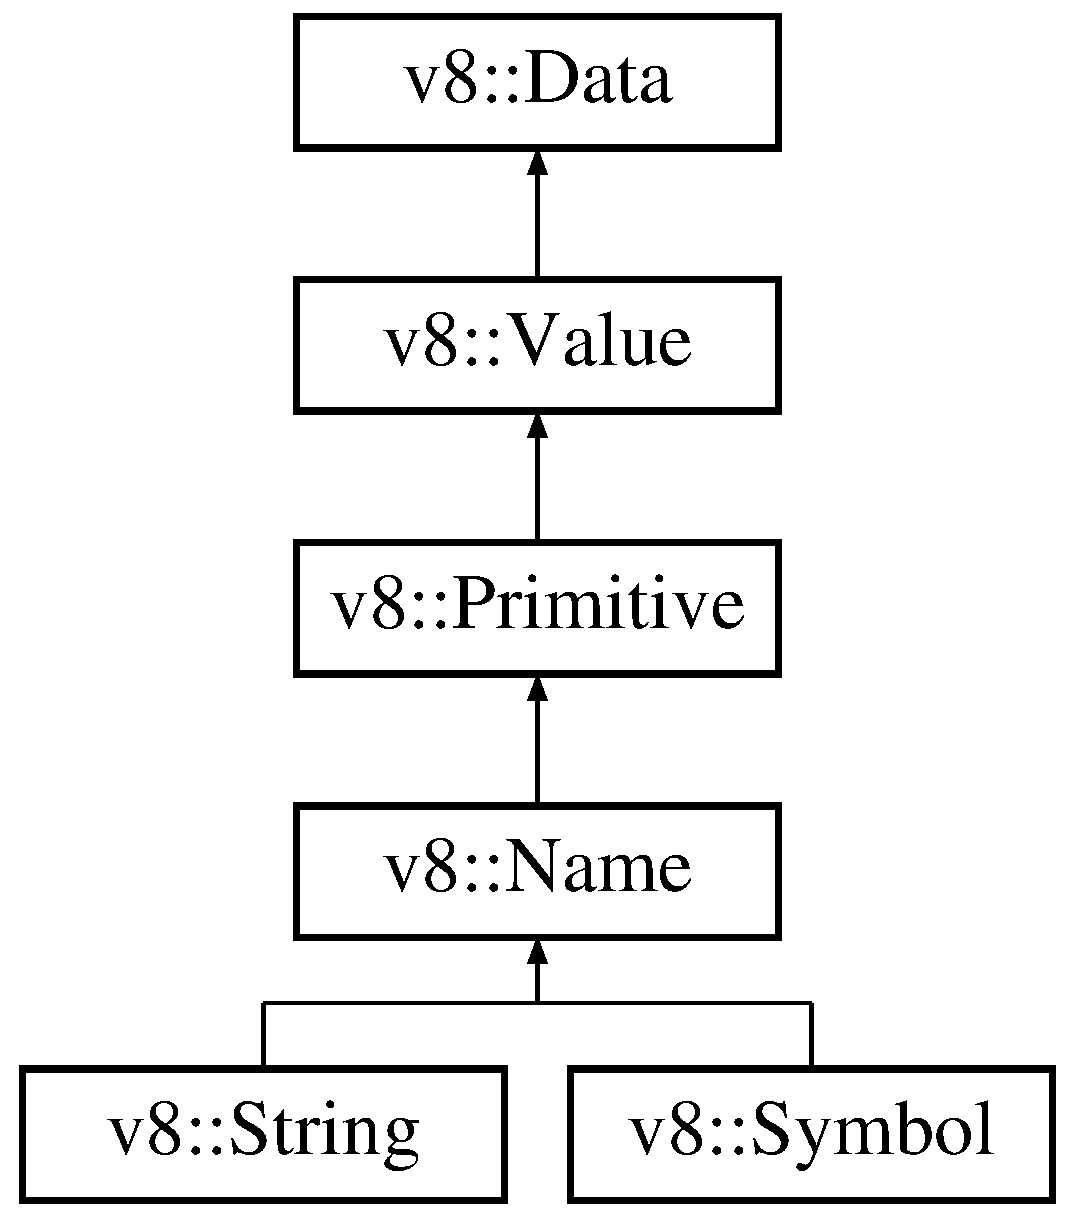
\includegraphics[height=5.000000cm]{classv8_1_1_name}
\end{center}
\end{figure}
\subsection*{Public Member Functions}
\begin{DoxyCompactItemize}
\item 
int \hyperlink{classv8_1_1_name_aef60fce47685fad12914304f6bc52bf2}{Get\+Identity\+Hash} ()
\end{DoxyCompactItemize}
\subsection*{Static Public Member Functions}
\begin{DoxyCompactItemize}
\item 
static V8\+\_\+\+I\+N\+L\+I\+NE \hyperlink{classv8_1_1_name}{Name} $\ast$ {\bfseries Cast} (\hyperlink{classv8_1_1_value}{v8\+::\+Value} $\ast$obj)\hypertarget{classv8_1_1_name_a8291aa8958f5dfb67d4415510f584ac4}{}\label{classv8_1_1_name_a8291aa8958f5dfb67d4415510f584ac4}

\end{DoxyCompactItemize}
\subsection*{Static Private Member Functions}
\begin{DoxyCompactItemize}
\item 
static void {\bfseries Check\+Cast} (\hyperlink{classv8_1_1_value}{v8\+::\+Value} $\ast$obj)\hypertarget{classv8_1_1_name_a9fbe24d05685553abbe386cf13219c08}{}\label{classv8_1_1_name_a9fbe24d05685553abbe386cf13219c08}

\end{DoxyCompactItemize}


\subsection{Detailed Description}
A superclass for symbols and strings. 

\subsection{Member Function Documentation}
\index{v8\+::\+Name@{v8\+::\+Name}!Get\+Identity\+Hash@{Get\+Identity\+Hash}}
\index{Get\+Identity\+Hash@{Get\+Identity\+Hash}!v8\+::\+Name@{v8\+::\+Name}}
\subsubsection[{\texorpdfstring{Get\+Identity\+Hash()}{GetIdentityHash()}}]{\setlength{\rightskip}{0pt plus 5cm}int v8\+::\+Name\+::\+Get\+Identity\+Hash (
\begin{DoxyParamCaption}
{}
\end{DoxyParamCaption}
)}\hypertarget{classv8_1_1_name_aef60fce47685fad12914304f6bc52bf2}{}\label{classv8_1_1_name_aef60fce47685fad12914304f6bc52bf2}
Returns the identity hash for this object. The current implementation uses an inline property on the object to store the identity hash.

The return value will never be 0. Also, it is not guaranteed to be unique. 

The documentation for this class was generated from the following file\+:\begin{DoxyCompactItemize}
\item 
/\+Users/joshgav/node/v8/include/v8.\+h\end{DoxyCompactItemize}

\hypertarget{structv8_1_1_jit_code_event_1_1name__t}{}\section{v8\+:\+:Jit\+Code\+Event\+:\+:name\+\_\+t Struct Reference}
\label{structv8_1_1_jit_code_event_1_1name__t}\index{v8\+::\+Jit\+Code\+Event\+::name\+\_\+t@{v8\+::\+Jit\+Code\+Event\+::name\+\_\+t}}
\subsection*{Public Attributes}
\begin{DoxyCompactItemize}
\item 
const char $\ast$ {\bfseries str}\hypertarget{structv8_1_1_jit_code_event_1_1name__t_a344732b4289a6a1fd21bb577ac9eff15}{}\label{structv8_1_1_jit_code_event_1_1name__t_a344732b4289a6a1fd21bb577ac9eff15}

\item 
size\+\_\+t {\bfseries len}\hypertarget{structv8_1_1_jit_code_event_1_1name__t_aa85ddd240f3b08c995caa8267ee8c586}{}\label{structv8_1_1_jit_code_event_1_1name__t_aa85ddd240f3b08c995caa8267ee8c586}

\end{DoxyCompactItemize}


The documentation for this struct was generated from the following file\+:\begin{DoxyCompactItemize}
\item 
/\+Users/joshgav/node/v8/include/v8.\+h\end{DoxyCompactItemize}

\hypertarget{structv8_1_1_named_property_handler_configuration}{}\section{v8\+:\+:Named\+Property\+Handler\+Configuration Struct Reference}
\label{structv8_1_1_named_property_handler_configuration}\index{v8\+::\+Named\+Property\+Handler\+Configuration@{v8\+::\+Named\+Property\+Handler\+Configuration}}
\subsection*{Public Member Functions}
\begin{DoxyCompactItemize}
\item 
\hyperlink{structv8_1_1_named_property_handler_configuration_a7304ee88edae7f7342f3a03f7974202d}{Named\+Property\+Handler\+Configuration} (\hyperlink{namespacev8_a24b1801fa53a7c5a71366d8044927563}{Generic\+Named\+Property\+Getter\+Callback} getter=0, \hyperlink{namespacev8_af74716c6e95a269c6cd4314662fd0a7e}{Generic\+Named\+Property\+Setter\+Callback} setter=0, \hyperlink{namespacev8_add9f7ab11e4a9a2b9ad2c4536b0e1a64}{Generic\+Named\+Property\+Query\+Callback} query=0, \hyperlink{namespacev8_ad2aecc0406ea4bc02d5a4f84a433b273}{Generic\+Named\+Property\+Deleter\+Callback} deleter=0, \hyperlink{namespacev8_a20826eb7e52e84fa4f632534e8eddd04}{Generic\+Named\+Property\+Enumerator\+Callback} enumerator=0, \hyperlink{classv8_1_1_local}{Local}$<$ \hyperlink{classv8_1_1_value}{Value} $>$ data=\hyperlink{classv8_1_1_local}{Local}$<$ \hyperlink{classv8_1_1_value}{Value} $>$(), Property\+Handler\+Flags flags=Property\+Handler\+Flags\+::k\+None)
\end{DoxyCompactItemize}
\subsection*{Public Attributes}
\begin{DoxyCompactItemize}
\item 
\hyperlink{namespacev8_a24b1801fa53a7c5a71366d8044927563}{Generic\+Named\+Property\+Getter\+Callback} {\bfseries getter}\hypertarget{structv8_1_1_named_property_handler_configuration_a7e0f2f6be4b716330f78e08dafb43512}{}\label{structv8_1_1_named_property_handler_configuration_a7e0f2f6be4b716330f78e08dafb43512}

\item 
\hyperlink{namespacev8_af74716c6e95a269c6cd4314662fd0a7e}{Generic\+Named\+Property\+Setter\+Callback} {\bfseries setter}\hypertarget{structv8_1_1_named_property_handler_configuration_a03a2c13ff0e66f02c5944620c38dcf61}{}\label{structv8_1_1_named_property_handler_configuration_a03a2c13ff0e66f02c5944620c38dcf61}

\item 
\hyperlink{namespacev8_add9f7ab11e4a9a2b9ad2c4536b0e1a64}{Generic\+Named\+Property\+Query\+Callback} {\bfseries query}\hypertarget{structv8_1_1_named_property_handler_configuration_af55d318e48d6f78b2103f3e603c86e34}{}\label{structv8_1_1_named_property_handler_configuration_af55d318e48d6f78b2103f3e603c86e34}

\item 
\hyperlink{namespacev8_ad2aecc0406ea4bc02d5a4f84a433b273}{Generic\+Named\+Property\+Deleter\+Callback} {\bfseries deleter}\hypertarget{structv8_1_1_named_property_handler_configuration_ab6f53889af636ead0218b02d3eda38c6}{}\label{structv8_1_1_named_property_handler_configuration_ab6f53889af636ead0218b02d3eda38c6}

\item 
\hyperlink{namespacev8_a20826eb7e52e84fa4f632534e8eddd04}{Generic\+Named\+Property\+Enumerator\+Callback} {\bfseries enumerator}\hypertarget{structv8_1_1_named_property_handler_configuration_a9d24735d39fe1486a4235ccc48333be7}{}\label{structv8_1_1_named_property_handler_configuration_a9d24735d39fe1486a4235ccc48333be7}

\item 
\hyperlink{classv8_1_1_local}{Local}$<$ \hyperlink{classv8_1_1_value}{Value} $>$ {\bfseries data}\hypertarget{structv8_1_1_named_property_handler_configuration_a209f02c8b3202551bb8eef448d750f9d}{}\label{structv8_1_1_named_property_handler_configuration_a209f02c8b3202551bb8eef448d750f9d}

\item 
Property\+Handler\+Flags {\bfseries flags}\hypertarget{structv8_1_1_named_property_handler_configuration_add28e99c72adf78b64e73f1de5aa74c7}{}\label{structv8_1_1_named_property_handler_configuration_add28e99c72adf78b64e73f1de5aa74c7}

\end{DoxyCompactItemize}


\subsection{Constructor \& Destructor Documentation}
\index{v8\+::\+Named\+Property\+Handler\+Configuration@{v8\+::\+Named\+Property\+Handler\+Configuration}!Named\+Property\+Handler\+Configuration@{Named\+Property\+Handler\+Configuration}}
\index{Named\+Property\+Handler\+Configuration@{Named\+Property\+Handler\+Configuration}!v8\+::\+Named\+Property\+Handler\+Configuration@{v8\+::\+Named\+Property\+Handler\+Configuration}}
\subsubsection[{\texorpdfstring{Named\+Property\+Handler\+Configuration(\+Generic\+Named\+Property\+Getter\+Callback getter=0, Generic\+Named\+Property\+Setter\+Callback setter=0, Generic\+Named\+Property\+Query\+Callback query=0, Generic\+Named\+Property\+Deleter\+Callback deleter=0, Generic\+Named\+Property\+Enumerator\+Callback enumerator=0, Local$<$ Value $>$ data=\+Local$<$ Value $>$(), Property\+Handler\+Flags flags=\+Property\+Handler\+Flags\+::k\+None)}{NamedPropertyHandlerConfiguration(GenericNamedPropertyGetterCallback getter=0, GenericNamedPropertySetterCallback setter=0, GenericNamedPropertyQueryCallback query=0, GenericNamedPropertyDeleterCallback deleter=0, GenericNamedPropertyEnumeratorCallback enumerator=0, Local< Value > data=Local< Value >(), PropertyHandlerFlags flags=PropertyHandlerFlags::kNone)}}]{\setlength{\rightskip}{0pt plus 5cm}v8\+::\+Named\+Property\+Handler\+Configuration\+::\+Named\+Property\+Handler\+Configuration (
\begin{DoxyParamCaption}
\item[{{\bf Generic\+Named\+Property\+Getter\+Callback}}]{getter = {\ttfamily 0}, }
\item[{{\bf Generic\+Named\+Property\+Setter\+Callback}}]{setter = {\ttfamily 0}, }
\item[{{\bf Generic\+Named\+Property\+Query\+Callback}}]{query = {\ttfamily 0}, }
\item[{{\bf Generic\+Named\+Property\+Deleter\+Callback}}]{deleter = {\ttfamily 0}, }
\item[{{\bf Generic\+Named\+Property\+Enumerator\+Callback}}]{enumerator = {\ttfamily 0}, }
\item[{{\bf Local}$<$ {\bf Value} $>$}]{data = {\ttfamily {\bf Local}$<${\bf Value}$>$()}, }
\item[{Property\+Handler\+Flags}]{flags = {\ttfamily PropertyHandlerFlags\+:\+:kNone}}
\end{DoxyParamCaption}
)\hspace{0.3cm}{\ttfamily [inline]}}\hypertarget{structv8_1_1_named_property_handler_configuration_a7304ee88edae7f7342f3a03f7974202d}{}\label{structv8_1_1_named_property_handler_configuration_a7304ee88edae7f7342f3a03f7974202d}

\begin{DoxyParams}{Parameters}
{\em getter} & Note\+: getter is required $\ast$ \\
\hline
\end{DoxyParams}


The documentation for this struct was generated from the following file\+:\begin{DoxyCompactItemize}
\item 
/\+Users/joshgav/node/v8/include/v8.\+h\end{DoxyCompactItemize}

\hypertarget{classv8_1_1_native_weak_map}{}\section{v8\+:\+:Native\+Weak\+Map Class Reference}
\label{classv8_1_1_native_weak_map}\index{v8\+::\+Native\+Weak\+Map@{v8\+::\+Native\+Weak\+Map}}


{\ttfamily \#include $<$v8.\+h$>$}

Inheritance diagram for v8\+:\+:Native\+Weak\+Map\+:\begin{figure}[H]
\begin{center}
\leavevmode
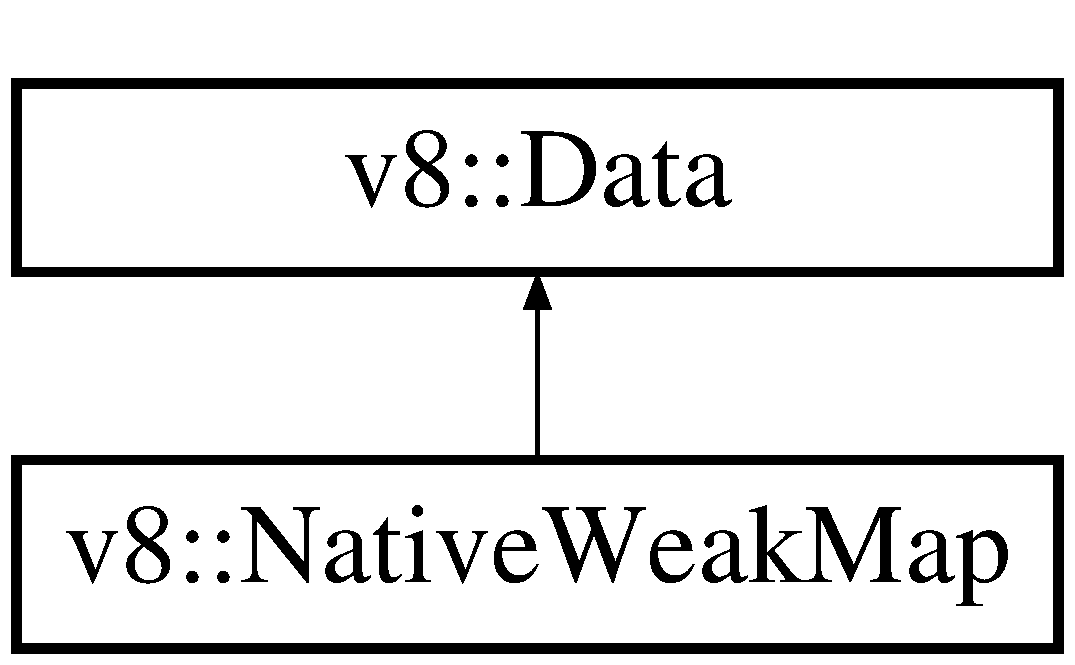
\includegraphics[height=2.000000cm]{classv8_1_1_native_weak_map}
\end{center}
\end{figure}
\subsection*{Public Member Functions}
\begin{DoxyCompactItemize}
\item 
void {\bfseries Set} (\hyperlink{classv8_1_1_local}{Local}$<$ \hyperlink{classv8_1_1_value}{Value} $>$ key, \hyperlink{classv8_1_1_local}{Local}$<$ \hyperlink{classv8_1_1_value}{Value} $>$ value)\hypertarget{classv8_1_1_native_weak_map_ade0e4ce74820a0fcf8b51fb1cea733a7}{}\label{classv8_1_1_native_weak_map_ade0e4ce74820a0fcf8b51fb1cea733a7}

\item 
\hyperlink{classv8_1_1_local}{Local}$<$ \hyperlink{classv8_1_1_value}{Value} $>$ {\bfseries Get} (\hyperlink{classv8_1_1_local}{Local}$<$ \hyperlink{classv8_1_1_value}{Value} $>$ key)\hypertarget{classv8_1_1_native_weak_map_aea031a4a1d529817d78c59b14325fc71}{}\label{classv8_1_1_native_weak_map_aea031a4a1d529817d78c59b14325fc71}

\item 
bool {\bfseries Has} (\hyperlink{classv8_1_1_local}{Local}$<$ \hyperlink{classv8_1_1_value}{Value} $>$ key)\hypertarget{classv8_1_1_native_weak_map_a9de62c6399280088c86bb57c3988e7cb}{}\label{classv8_1_1_native_weak_map_a9de62c6399280088c86bb57c3988e7cb}

\item 
bool {\bfseries Delete} (\hyperlink{classv8_1_1_local}{Local}$<$ \hyperlink{classv8_1_1_value}{Value} $>$ key)\hypertarget{classv8_1_1_native_weak_map_ae3c04eaa9e745732f7b2f16c6e75dead}{}\label{classv8_1_1_native_weak_map_ae3c04eaa9e745732f7b2f16c6e75dead}

\end{DoxyCompactItemize}
\subsection*{Static Public Member Functions}
\begin{DoxyCompactItemize}
\item 
static \hyperlink{classv8_1_1_local}{Local}$<$ \hyperlink{classv8_1_1_native_weak_map}{Native\+Weak\+Map} $>$ {\bfseries New} (\hyperlink{classv8_1_1_isolate}{Isolate} $\ast$isolate)\hypertarget{classv8_1_1_native_weak_map_af59b34fd9c1a4e1488fdf7f0709880e6}{}\label{classv8_1_1_native_weak_map_af59b34fd9c1a4e1488fdf7f0709880e6}

\end{DoxyCompactItemize}


\subsection{Detailed Description}
A map whose keys are referenced weakly. It is similar to Java\+Script Weak\+Map but can be created without entering a \hyperlink{classv8_1_1_context}{v8\+::\+Context} and hence shouldn\textquotesingle{}t escape to Java\+Script. 

The documentation for this class was generated from the following files\+:\begin{DoxyCompactItemize}
\item 
/\+Users/joshgav/node/v8/include/v8.\+h\item 
/\+Users/joshgav/node/v8/src/api.\+cc\end{DoxyCompactItemize}

\hypertarget{structv8_1_1_allocation_profile_1_1_node}{}\section{v8\+:\+:Allocation\+Profile\+:\+:Node Struct Reference}
\label{structv8_1_1_allocation_profile_1_1_node}\index{v8\+::\+Allocation\+Profile\+::\+Node@{v8\+::\+Allocation\+Profile\+::\+Node}}


{\ttfamily \#include $<$v8-\/profiler.\+h$>$}

\subsection*{Public Attributes}
\begin{DoxyCompactItemize}
\item 
\hyperlink{classv8_1_1_local}{Local}$<$ \hyperlink{classv8_1_1_string}{String} $>$ \hyperlink{structv8_1_1_allocation_profile_1_1_node_af9f2c323d6a11e836c02e8ac88adc5a8}{name}
\item 
\hyperlink{classv8_1_1_local}{Local}$<$ \hyperlink{classv8_1_1_string}{String} $>$ \hyperlink{structv8_1_1_allocation_profile_1_1_node_acd6567ac06a0bae713390559128e9c62}{script\+\_\+name}
\item 
int \hyperlink{structv8_1_1_allocation_profile_1_1_node_a4a746de878d9ad42b32fda4c365b98fb}{script\+\_\+id}
\item 
int \hyperlink{structv8_1_1_allocation_profile_1_1_node_a6caceefbf826a0425adc74331cc7a910}{start\+\_\+position}
\item 
int \hyperlink{structv8_1_1_allocation_profile_1_1_node_ac9773c92a3af3a9a9420337599e68bd9}{line\+\_\+number}
\item 
int \hyperlink{structv8_1_1_allocation_profile_1_1_node_a7cf86acc298428c858673fc1f9dbe305}{column\+\_\+number}
\item 
std\+::vector$<$ \hyperlink{structv8_1_1_allocation_profile_1_1_node}{Node} $\ast$ $>$ \hyperlink{structv8_1_1_allocation_profile_1_1_node_a176673c0440cb1baaf7713e14da84db0}{children}
\item 
std\+::vector$<$ \hyperlink{structv8_1_1_allocation_profile_1_1_allocation}{Allocation} $>$ \hyperlink{structv8_1_1_allocation_profile_1_1_node_a6ee0934b35ba77fb5d8b53f02d5a3068}{allocations}
\end{DoxyCompactItemize}


\subsection{Detailed Description}
Represents a node in the call-\/graph. 

\subsection{Member Data Documentation}
\index{v8\+::\+Allocation\+Profile\+::\+Node@{v8\+::\+Allocation\+Profile\+::\+Node}!allocations@{allocations}}
\index{allocations@{allocations}!v8\+::\+Allocation\+Profile\+::\+Node@{v8\+::\+Allocation\+Profile\+::\+Node}}
\subsubsection[{\texorpdfstring{allocations}{allocations}}]{\setlength{\rightskip}{0pt plus 5cm}std\+::vector$<${\bf Allocation}$>$ v8\+::\+Allocation\+Profile\+::\+Node\+::allocations}\hypertarget{structv8_1_1_allocation_profile_1_1_node_a6ee0934b35ba77fb5d8b53f02d5a3068}{}\label{structv8_1_1_allocation_profile_1_1_node_a6ee0934b35ba77fb5d8b53f02d5a3068}
List of self allocations done by this node in the call-\/graph. \index{v8\+::\+Allocation\+Profile\+::\+Node@{v8\+::\+Allocation\+Profile\+::\+Node}!children@{children}}
\index{children@{children}!v8\+::\+Allocation\+Profile\+::\+Node@{v8\+::\+Allocation\+Profile\+::\+Node}}
\subsubsection[{\texorpdfstring{children}{children}}]{\setlength{\rightskip}{0pt plus 5cm}std\+::vector$<${\bf Node}$\ast$$>$ v8\+::\+Allocation\+Profile\+::\+Node\+::children}\hypertarget{structv8_1_1_allocation_profile_1_1_node_a176673c0440cb1baaf7713e14da84db0}{}\label{structv8_1_1_allocation_profile_1_1_node_a176673c0440cb1baaf7713e14da84db0}
List of callees called from this node for which we have sampled allocations. The lifetime of the children is scoped to the containing \hyperlink{classv8_1_1_allocation_profile}{Allocation\+Profile}. \index{v8\+::\+Allocation\+Profile\+::\+Node@{v8\+::\+Allocation\+Profile\+::\+Node}!column\+\_\+number@{column\+\_\+number}}
\index{column\+\_\+number@{column\+\_\+number}!v8\+::\+Allocation\+Profile\+::\+Node@{v8\+::\+Allocation\+Profile\+::\+Node}}
\subsubsection[{\texorpdfstring{column\+\_\+number}{column_number}}]{\setlength{\rightskip}{0pt plus 5cm}int v8\+::\+Allocation\+Profile\+::\+Node\+::column\+\_\+number}\hypertarget{structv8_1_1_allocation_profile_1_1_node_a7cf86acc298428c858673fc1f9dbe305}{}\label{structv8_1_1_allocation_profile_1_1_node_a7cf86acc298428c858673fc1f9dbe305}
1-\/indexed column number where the function starts. May be k\+No\+Column\+Number\+Info if no line number information is available. \index{v8\+::\+Allocation\+Profile\+::\+Node@{v8\+::\+Allocation\+Profile\+::\+Node}!line\+\_\+number@{line\+\_\+number}}
\index{line\+\_\+number@{line\+\_\+number}!v8\+::\+Allocation\+Profile\+::\+Node@{v8\+::\+Allocation\+Profile\+::\+Node}}
\subsubsection[{\texorpdfstring{line\+\_\+number}{line_number}}]{\setlength{\rightskip}{0pt plus 5cm}int v8\+::\+Allocation\+Profile\+::\+Node\+::line\+\_\+number}\hypertarget{structv8_1_1_allocation_profile_1_1_node_ac9773c92a3af3a9a9420337599e68bd9}{}\label{structv8_1_1_allocation_profile_1_1_node_ac9773c92a3af3a9a9420337599e68bd9}
1-\/indexed line number where the function starts. May be k\+No\+Line\+Number\+Info if no line number information is available. \index{v8\+::\+Allocation\+Profile\+::\+Node@{v8\+::\+Allocation\+Profile\+::\+Node}!name@{name}}
\index{name@{name}!v8\+::\+Allocation\+Profile\+::\+Node@{v8\+::\+Allocation\+Profile\+::\+Node}}
\subsubsection[{\texorpdfstring{name}{name}}]{\setlength{\rightskip}{0pt plus 5cm}{\bf Local}$<${\bf String}$>$ v8\+::\+Allocation\+Profile\+::\+Node\+::name}\hypertarget{structv8_1_1_allocation_profile_1_1_node_af9f2c323d6a11e836c02e8ac88adc5a8}{}\label{structv8_1_1_allocation_profile_1_1_node_af9f2c323d6a11e836c02e8ac88adc5a8}
\hyperlink{classv8_1_1_name}{Name} of the function. May be empty for anonymous functions or if the script corresponding to this function has been unloaded. \index{v8\+::\+Allocation\+Profile\+::\+Node@{v8\+::\+Allocation\+Profile\+::\+Node}!script\+\_\+id@{script\+\_\+id}}
\index{script\+\_\+id@{script\+\_\+id}!v8\+::\+Allocation\+Profile\+::\+Node@{v8\+::\+Allocation\+Profile\+::\+Node}}
\subsubsection[{\texorpdfstring{script\+\_\+id}{script_id}}]{\setlength{\rightskip}{0pt plus 5cm}int v8\+::\+Allocation\+Profile\+::\+Node\+::script\+\_\+id}\hypertarget{structv8_1_1_allocation_profile_1_1_node_a4a746de878d9ad42b32fda4c365b98fb}{}\label{structv8_1_1_allocation_profile_1_1_node_a4a746de878d9ad42b32fda4c365b98fb}
id of the script where the function is located. May be equal to v8\+::\+Unbound\+Script\+::k\+No\+Script\+Id in cases where the script doesn\textquotesingle{}t exist. \index{v8\+::\+Allocation\+Profile\+::\+Node@{v8\+::\+Allocation\+Profile\+::\+Node}!script\+\_\+name@{script\+\_\+name}}
\index{script\+\_\+name@{script\+\_\+name}!v8\+::\+Allocation\+Profile\+::\+Node@{v8\+::\+Allocation\+Profile\+::\+Node}}
\subsubsection[{\texorpdfstring{script\+\_\+name}{script_name}}]{\setlength{\rightskip}{0pt plus 5cm}{\bf Local}$<${\bf String}$>$ v8\+::\+Allocation\+Profile\+::\+Node\+::script\+\_\+name}\hypertarget{structv8_1_1_allocation_profile_1_1_node_acd6567ac06a0bae713390559128e9c62}{}\label{structv8_1_1_allocation_profile_1_1_node_acd6567ac06a0bae713390559128e9c62}
\hyperlink{classv8_1_1_name}{Name} of the script containing the function. May be empty if the script name is not available, or if the script has been unloaded. \index{v8\+::\+Allocation\+Profile\+::\+Node@{v8\+::\+Allocation\+Profile\+::\+Node}!start\+\_\+position@{start\+\_\+position}}
\index{start\+\_\+position@{start\+\_\+position}!v8\+::\+Allocation\+Profile\+::\+Node@{v8\+::\+Allocation\+Profile\+::\+Node}}
\subsubsection[{\texorpdfstring{start\+\_\+position}{start_position}}]{\setlength{\rightskip}{0pt plus 5cm}int v8\+::\+Allocation\+Profile\+::\+Node\+::start\+\_\+position}\hypertarget{structv8_1_1_allocation_profile_1_1_node_a6caceefbf826a0425adc74331cc7a910}{}\label{structv8_1_1_allocation_profile_1_1_node_a6caceefbf826a0425adc74331cc7a910}
Start position of the function in the script. 

The documentation for this struct was generated from the following file\+:\begin{DoxyCompactItemize}
\item 
/\+Users/joshgav/node/v8/include/v8-\/profiler.\+h\end{DoxyCompactItemize}

\hypertarget{classv8_1_1_non_copyable_persistent_traits}{}\section{v8\+:\+:Non\+Copyable\+Persistent\+Traits$<$ T $>$ Class Template Reference}
\label{classv8_1_1_non_copyable_persistent_traits}\index{v8\+::\+Non\+Copyable\+Persistent\+Traits$<$ T $>$@{v8\+::\+Non\+Copyable\+Persistent\+Traits$<$ T $>$}}


{\ttfamily \#include $<$v8.\+h$>$}

\subsection*{Public Types}
\begin{DoxyCompactItemize}
\item 
typedef \hyperlink{classv8_1_1_persistent}{Persistent}$<$ T, \hyperlink{classv8_1_1_non_copyable_persistent_traits}{Non\+Copyable\+Persistent\+Traits}$<$ T $>$ $>$ {\bfseries Non\+Copyable\+Persistent}\hypertarget{classv8_1_1_non_copyable_persistent_traits_af26082b31726b82c0482a01daa2f3e54}{}\label{classv8_1_1_non_copyable_persistent_traits_af26082b31726b82c0482a01daa2f3e54}

\end{DoxyCompactItemize}
\subsection*{Static Public Member Functions}
\begin{DoxyCompactItemize}
\item 
{\footnotesize template$<$class S , class M $>$ }\\static V8\+\_\+\+I\+N\+L\+I\+NE void {\bfseries Copy} (const \hyperlink{classv8_1_1_persistent}{Persistent}$<$ S, M $>$ \&source, \hyperlink{classv8_1_1_persistent}{Non\+Copyable\+Persistent} $\ast$dest)\hypertarget{classv8_1_1_non_copyable_persistent_traits_a40b133b17a334c5c7674135e7dbcf850}{}\label{classv8_1_1_non_copyable_persistent_traits_a40b133b17a334c5c7674135e7dbcf850}

\item 
{\footnotesize template$<$class O $>$ }\\static V8\+\_\+\+I\+N\+L\+I\+NE void {\bfseries Uncompilable} ()\hypertarget{classv8_1_1_non_copyable_persistent_traits_a90e2c6958ba089f5fabbbc7c08f976c1}{}\label{classv8_1_1_non_copyable_persistent_traits_a90e2c6958ba089f5fabbbc7c08f976c1}

\end{DoxyCompactItemize}
\subsection*{Static Public Attributes}
\begin{DoxyCompactItemize}
\item 
static const bool {\bfseries k\+Reset\+In\+Destructor} = false\hypertarget{classv8_1_1_non_copyable_persistent_traits_a650880d85ff80634c30a195d20329681}{}\label{classv8_1_1_non_copyable_persistent_traits_a650880d85ff80634c30a195d20329681}

\end{DoxyCompactItemize}


\subsection{Detailed Description}
\subsubsection*{template$<$class T$>$\\*
class v8\+::\+Non\+Copyable\+Persistent\+Traits$<$ T $>$}

Default traits for \hyperlink{classv8_1_1_persistent}{Persistent}. This class does not allow use of the copy constructor or assignment operator. At present k\+Reset\+In\+Destructor is not set, but that will change in a future version. 

The documentation for this class was generated from the following file\+:\begin{DoxyCompactItemize}
\item 
/\+Users/joshgav/node/v8/include/v8.\+h\end{DoxyCompactItemize}

\hypertarget{classv8_1_1_number}{}\section{v8\+:\+:Number Class Reference}
\label{classv8_1_1_number}\index{v8\+::\+Number@{v8\+::\+Number}}


{\ttfamily \#include $<$v8.\+h$>$}

Inheritance diagram for v8\+:\+:Number\+:\begin{figure}[H]
\begin{center}
\leavevmode
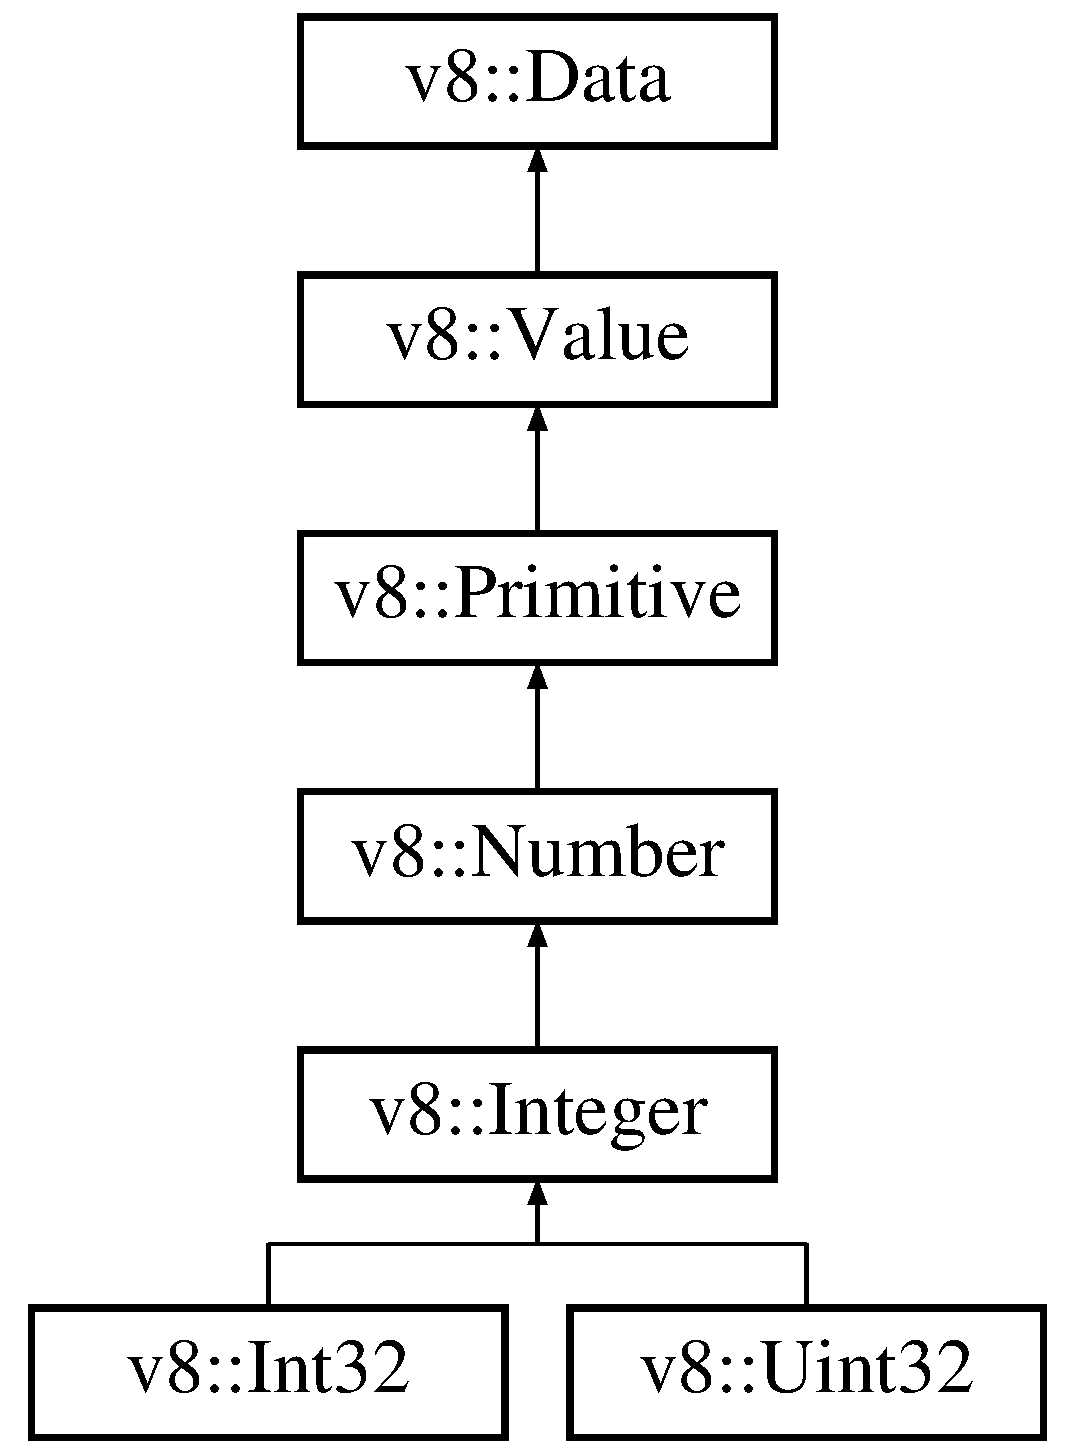
\includegraphics[height=6.000000cm]{classv8_1_1_number}
\end{center}
\end{figure}
\subsection*{Public Member Functions}
\begin{DoxyCompactItemize}
\item 
double {\bfseries Value} () const \hypertarget{classv8_1_1_number_ae7ca1af5dd34a7a32a69f57a910ab269}{}\label{classv8_1_1_number_ae7ca1af5dd34a7a32a69f57a910ab269}

\end{DoxyCompactItemize}
\subsection*{Static Public Member Functions}
\begin{DoxyCompactItemize}
\item 
static \hyperlink{classv8_1_1_local}{Local}$<$ \hyperlink{classv8_1_1_number}{Number} $>$ {\bfseries New} (\hyperlink{classv8_1_1_isolate}{Isolate} $\ast$isolate, double value)\hypertarget{classv8_1_1_number_a90ea55018560648ffaf8861372b41928}{}\label{classv8_1_1_number_a90ea55018560648ffaf8861372b41928}

\item 
static V8\+\_\+\+I\+N\+L\+I\+NE \hyperlink{classv8_1_1_number}{Number} $\ast$ {\bfseries Cast} (\hyperlink{classv8_1_1_value}{v8\+::\+Value} $\ast$obj)\hypertarget{classv8_1_1_number_a053d48e0003104308963a4a7e3881912}{}\label{classv8_1_1_number_a053d48e0003104308963a4a7e3881912}

\end{DoxyCompactItemize}
\subsection*{Static Private Member Functions}
\begin{DoxyCompactItemize}
\item 
static void {\bfseries Check\+Cast} (\hyperlink{classv8_1_1_value}{v8\+::\+Value} $\ast$obj)\hypertarget{classv8_1_1_number_a722d1cad74dd79ab1653fecc8c3dafa7}{}\label{classv8_1_1_number_a722d1cad74dd79ab1653fecc8c3dafa7}

\end{DoxyCompactItemize}


\subsection{Detailed Description}
A Java\+Script number value (E\+C\+M\+A-\/262, 4.\+3.\+20) 

The documentation for this class was generated from the following file\+:\begin{DoxyCompactItemize}
\item 
/\+Users/joshgav/node/v8/include/v8.\+h\end{DoxyCompactItemize}

\hypertarget{classv8_1_1_number_object}{}\section{v8\+:\+:Number\+Object Class Reference}
\label{classv8_1_1_number_object}\index{v8\+::\+Number\+Object@{v8\+::\+Number\+Object}}


{\ttfamily \#include $<$v8.\+h$>$}

Inheritance diagram for v8\+:\+:Number\+Object\+:\begin{figure}[H]
\begin{center}
\leavevmode
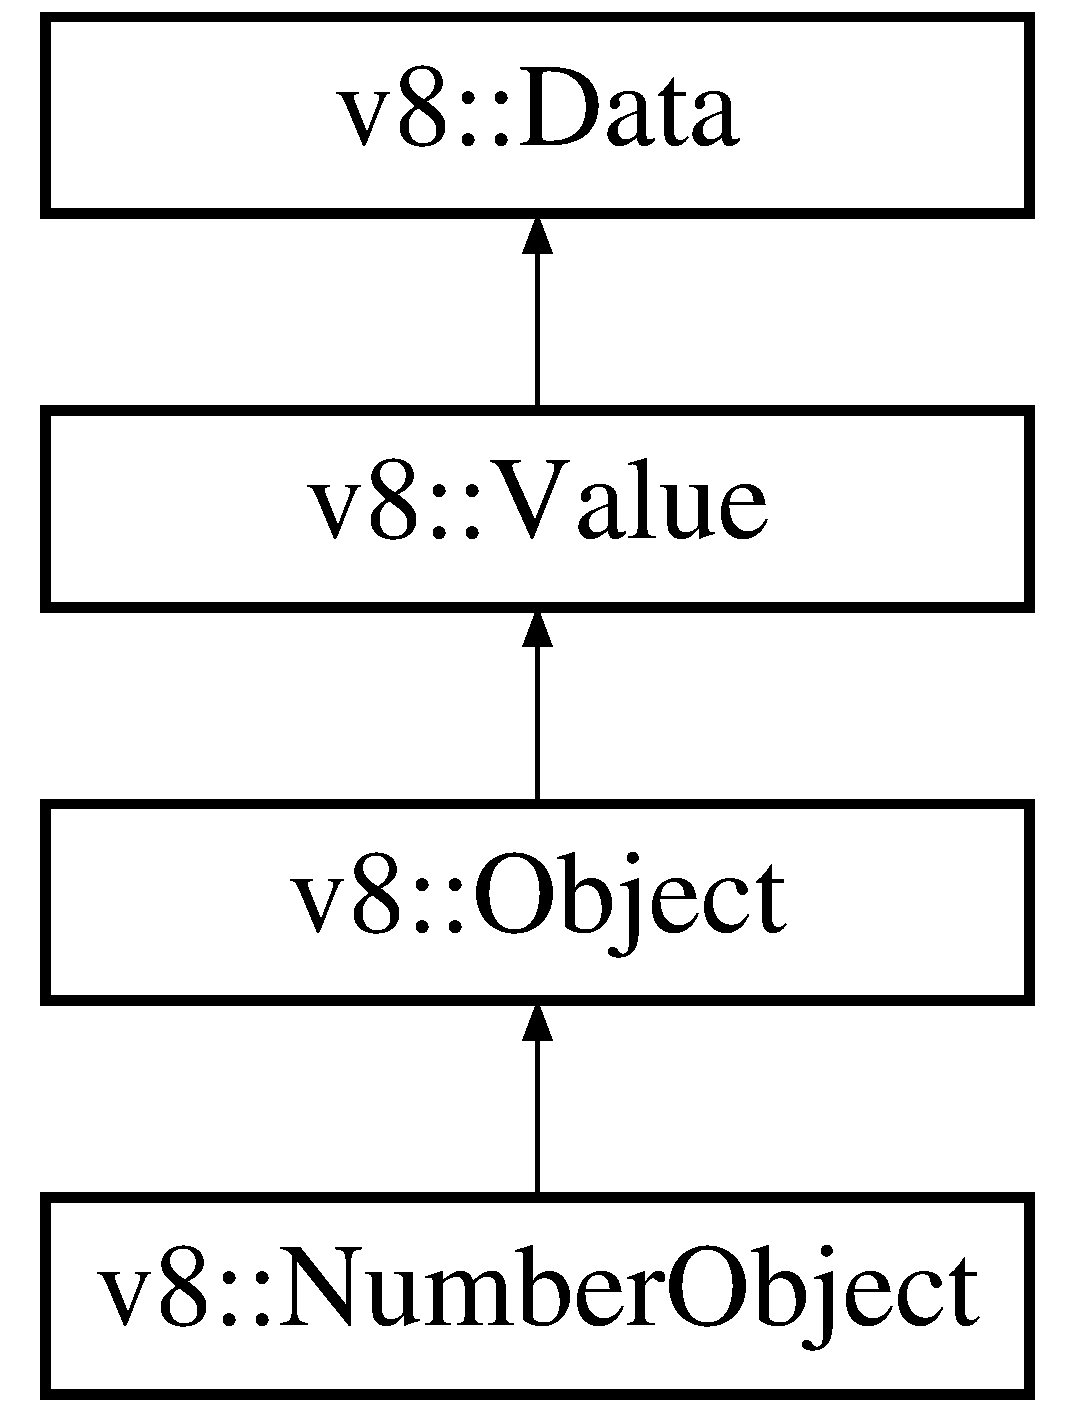
\includegraphics[height=4.000000cm]{classv8_1_1_number_object}
\end{center}
\end{figure}
\subsection*{Public Member Functions}
\begin{DoxyCompactItemize}
\item 
double {\bfseries Value\+Of} () const \hypertarget{classv8_1_1_number_object_a40c7211d55bc2de1b23f475d1906b5bf}{}\label{classv8_1_1_number_object_a40c7211d55bc2de1b23f475d1906b5bf}

\end{DoxyCompactItemize}
\subsection*{Static Public Member Functions}
\begin{DoxyCompactItemize}
\item 
static \hyperlink{classv8_1_1_local}{Local}$<$ \hyperlink{classv8_1_1_value}{Value} $>$ {\bfseries New} (\hyperlink{classv8_1_1_isolate}{Isolate} $\ast$isolate, double value)\hypertarget{classv8_1_1_number_object_afada011e39331dab09261e81b349c4a2}{}\label{classv8_1_1_number_object_afada011e39331dab09261e81b349c4a2}

\item 
static V8\+\_\+\+I\+N\+L\+I\+NE \hyperlink{classv8_1_1_number_object}{Number\+Object} $\ast$ {\bfseries Cast} (\hyperlink{classv8_1_1_value}{v8\+::\+Value} $\ast$obj)\hypertarget{classv8_1_1_number_object_a0dad558fde0ec8e51ff53a3e34dbce7e}{}\label{classv8_1_1_number_object_a0dad558fde0ec8e51ff53a3e34dbce7e}

\end{DoxyCompactItemize}
\subsection*{Static Private Member Functions}
\begin{DoxyCompactItemize}
\item 
static void {\bfseries Check\+Cast} (\hyperlink{classv8_1_1_value}{v8\+::\+Value} $\ast$obj)\hypertarget{classv8_1_1_number_object_aeb7ab9979b521950db16ba4b0a3a8057}{}\label{classv8_1_1_number_object_aeb7ab9979b521950db16ba4b0a3a8057}

\end{DoxyCompactItemize}


\subsection{Detailed Description}
A \hyperlink{classv8_1_1_number}{Number} object (E\+C\+M\+A-\/262, 4.\+3.\+21). 

The documentation for this class was generated from the following files\+:\begin{DoxyCompactItemize}
\item 
/\+Users/joshgav/node/v8/include/v8.\+h\item 
/\+Users/joshgav/node/v8/src/api.\+cc\end{DoxyCompactItemize}

\hypertarget{classv8_1_1_object}{}\section{v8\+:\+:Object Class Reference}
\label{classv8_1_1_object}\index{v8\+::\+Object@{v8\+::\+Object}}


{\ttfamily \#include $<$v8.\+h$>$}

Inheritance diagram for v8\+:\+:Object\+:\begin{figure}[H]
\begin{center}
\leavevmode
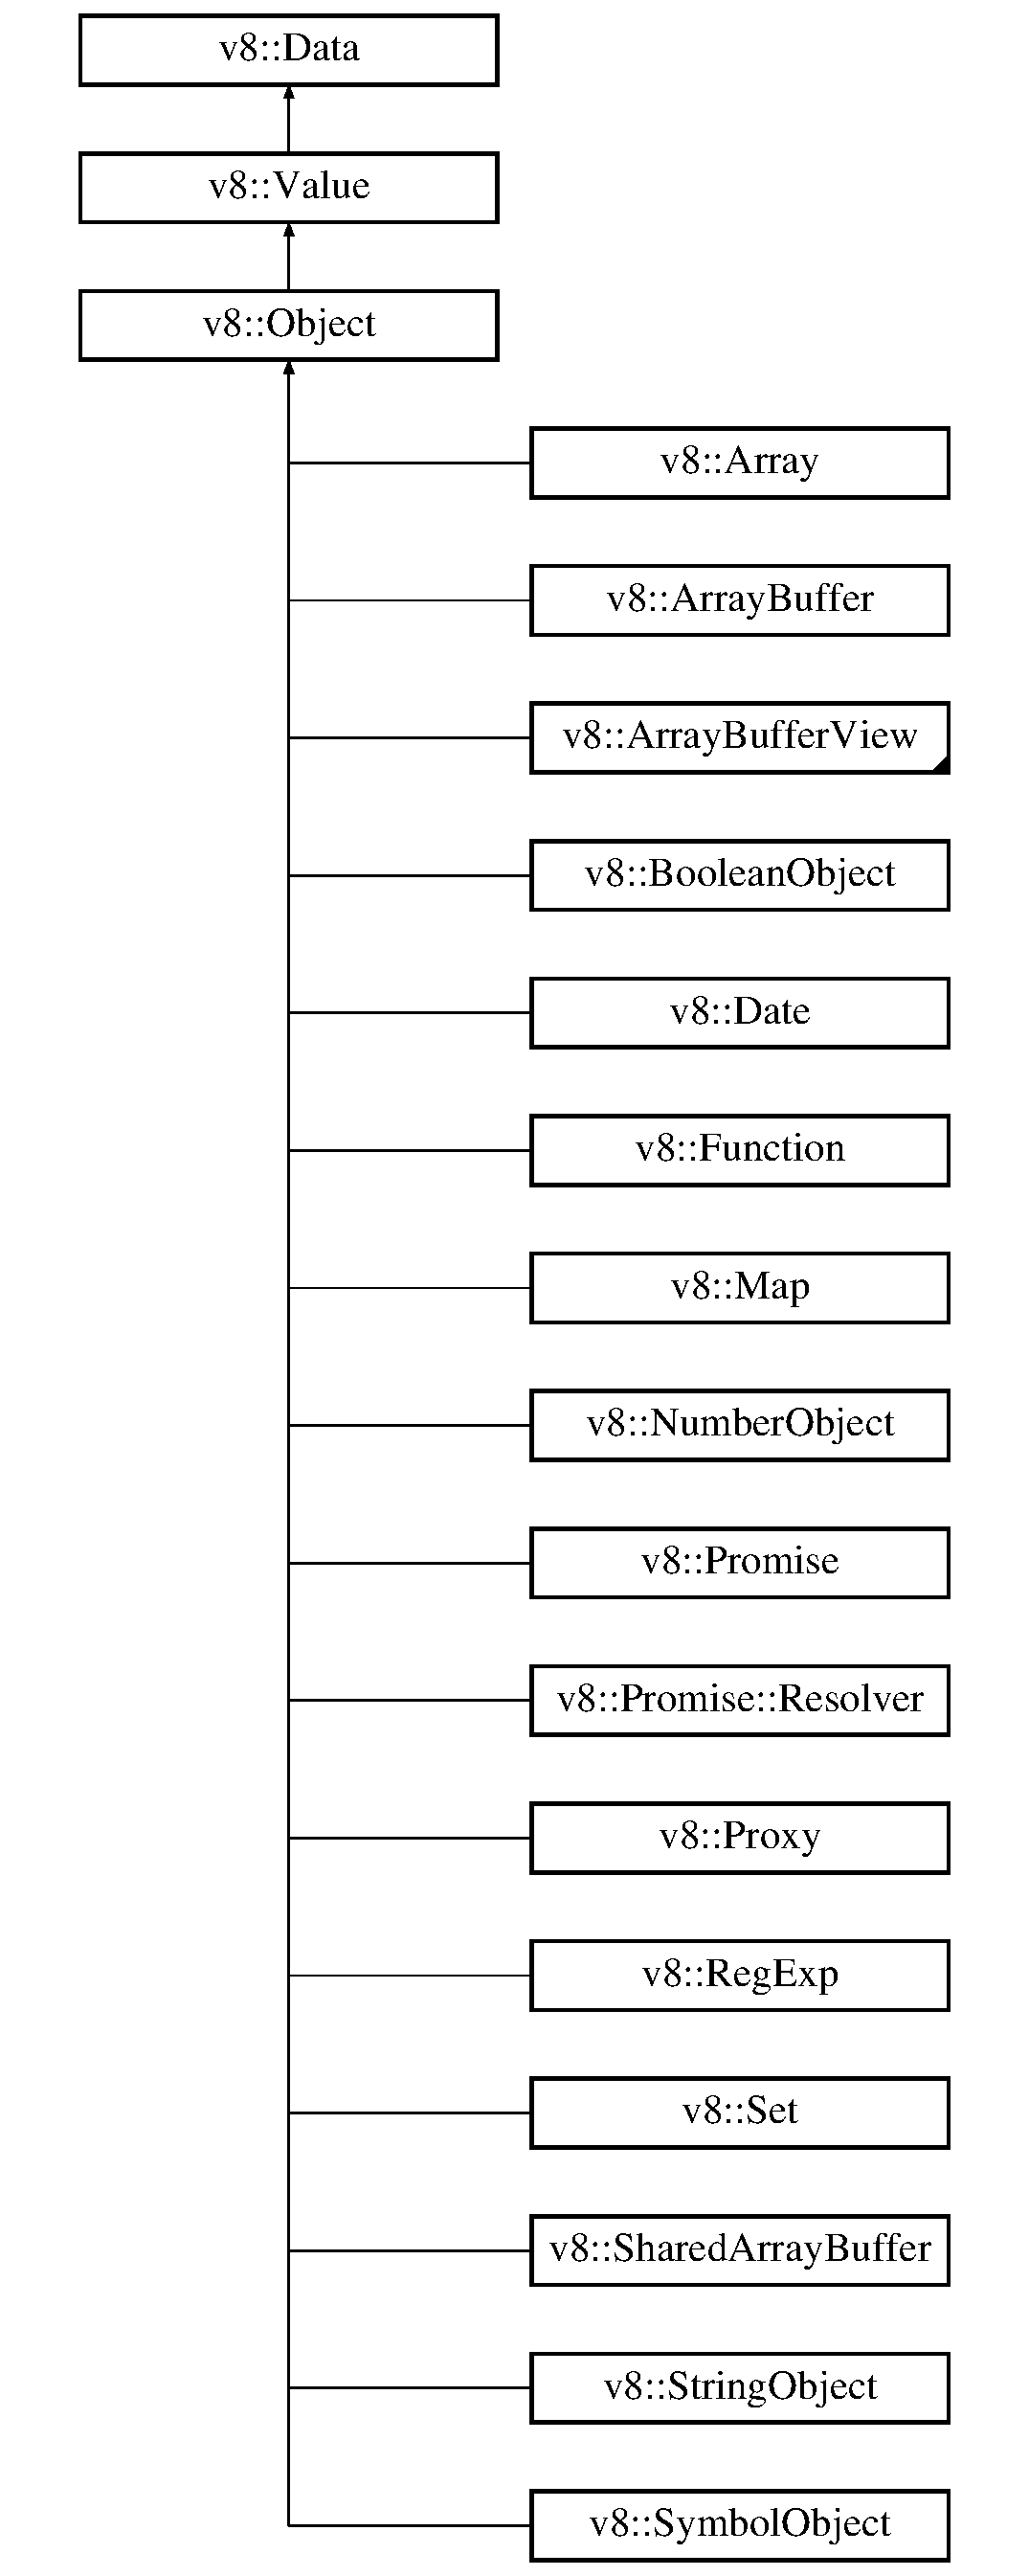
\includegraphics[height=12.000000cm]{classv8_1_1_object}
\end{center}
\end{figure}
\subsection*{Public Member Functions}
\begin{DoxyCompactItemize}
\item 
{\bfseries V8\+\_\+\+D\+E\+P\+R\+E\+C\+A\+T\+E\+\_\+\+S\+O\+ON} (\char`\"{}Use maybe version\char`\"{}, bool \hyperlink{classv8_1_1_set}{Set}(\hyperlink{classv8_1_1_local}{Local}$<$ \hyperlink{classv8_1_1_value}{Value} $>$ key, \hyperlink{classv8_1_1_local}{Local}$<$ \hyperlink{classv8_1_1_value}{Value} $>$ value))\hypertarget{classv8_1_1_object_a86333122230b703cabfb08d8a7d54a58}{}\label{classv8_1_1_object_a86333122230b703cabfb08d8a7d54a58}

\item 
V8\+\_\+\+W\+A\+R\+N\+\_\+\+U\+N\+U\+S\+E\+D\+\_\+\+R\+E\+S\+U\+LT \hyperlink{classv8_1_1_maybe}{Maybe}$<$ bool $>$ {\bfseries Set} (\hyperlink{classv8_1_1_local}{Local}$<$ \hyperlink{classv8_1_1_context}{Context} $>$ context, \hyperlink{classv8_1_1_local}{Local}$<$ \hyperlink{classv8_1_1_value}{Value} $>$ key, \hyperlink{classv8_1_1_local}{Local}$<$ \hyperlink{classv8_1_1_value}{Value} $>$ value)\hypertarget{classv8_1_1_object_ac5840fc655bea7b2b55a4b49338360ae}{}\label{classv8_1_1_object_ac5840fc655bea7b2b55a4b49338360ae}

\item 
{\bfseries V8\+\_\+\+D\+E\+P\+R\+E\+C\+A\+T\+E\+\_\+\+S\+O\+ON} (\char`\"{}Use maybe version\char`\"{}, bool \hyperlink{classv8_1_1_set}{Set}(uint32\+\_\+t index, \hyperlink{classv8_1_1_local}{Local}$<$ \hyperlink{classv8_1_1_value}{Value} $>$ value))\hypertarget{classv8_1_1_object_a0c2305335e71c88d245dd1aa0060a2de}{}\label{classv8_1_1_object_a0c2305335e71c88d245dd1aa0060a2de}

\item 
V8\+\_\+\+W\+A\+R\+N\+\_\+\+U\+N\+U\+S\+E\+D\+\_\+\+R\+E\+S\+U\+LT \hyperlink{classv8_1_1_maybe}{Maybe}$<$ bool $>$ {\bfseries Set} (\hyperlink{classv8_1_1_local}{Local}$<$ \hyperlink{classv8_1_1_context}{Context} $>$ context, uint32\+\_\+t index, \hyperlink{classv8_1_1_local}{Local}$<$ \hyperlink{classv8_1_1_value}{Value} $>$ value)\hypertarget{classv8_1_1_object_ace0cbcf5659a82106601d07b3e6fa2be}{}\label{classv8_1_1_object_ace0cbcf5659a82106601d07b3e6fa2be}

\item 
V8\+\_\+\+W\+A\+R\+N\+\_\+\+U\+N\+U\+S\+E\+D\+\_\+\+R\+E\+S\+U\+LT \hyperlink{classv8_1_1_maybe}{Maybe}$<$ bool $>$ {\bfseries Create\+Data\+Property} (\hyperlink{classv8_1_1_local}{Local}$<$ \hyperlink{classv8_1_1_context}{Context} $>$ context, \hyperlink{classv8_1_1_local}{Local}$<$ \hyperlink{classv8_1_1_name}{Name} $>$ key, \hyperlink{classv8_1_1_local}{Local}$<$ \hyperlink{classv8_1_1_value}{Value} $>$ value)\hypertarget{classv8_1_1_object_ae334696b1e57ea2b333c4da48dd37895}{}\label{classv8_1_1_object_ae334696b1e57ea2b333c4da48dd37895}

\item 
V8\+\_\+\+W\+A\+R\+N\+\_\+\+U\+N\+U\+S\+E\+D\+\_\+\+R\+E\+S\+U\+LT \hyperlink{classv8_1_1_maybe}{Maybe}$<$ bool $>$ {\bfseries Create\+Data\+Property} (\hyperlink{classv8_1_1_local}{Local}$<$ \hyperlink{classv8_1_1_context}{Context} $>$ context, uint32\+\_\+t index, \hyperlink{classv8_1_1_local}{Local}$<$ \hyperlink{classv8_1_1_value}{Value} $>$ value)\hypertarget{classv8_1_1_object_aec3a99813837c0bc6444c59f8e5ca22a}{}\label{classv8_1_1_object_aec3a99813837c0bc6444c59f8e5ca22a}

\item 
V8\+\_\+\+W\+A\+R\+N\+\_\+\+U\+N\+U\+S\+E\+D\+\_\+\+R\+E\+S\+U\+LT \hyperlink{classv8_1_1_maybe}{Maybe}$<$ bool $>$ {\bfseries Define\+Own\+Property} (\hyperlink{classv8_1_1_local}{Local}$<$ \hyperlink{classv8_1_1_context}{Context} $>$ context, \hyperlink{classv8_1_1_local}{Local}$<$ \hyperlink{classv8_1_1_name}{Name} $>$ key, \hyperlink{classv8_1_1_local}{Local}$<$ \hyperlink{classv8_1_1_value}{Value} $>$ value, Property\+Attribute attributes=None)\hypertarget{classv8_1_1_object_a65f44f92b7ee9d479ce6b3ebb9ac8d4b}{}\label{classv8_1_1_object_a65f44f92b7ee9d479ce6b3ebb9ac8d4b}

\item 
{\bfseries V8\+\_\+\+D\+E\+P\+R\+E\+C\+A\+T\+ED} (\char`\"{}Use Create\+Data\+Property / Define\+Own\+Property\char`\"{}, bool Force\+Set(\hyperlink{classv8_1_1_local}{Local}$<$ \hyperlink{classv8_1_1_value}{Value} $>$ key, \hyperlink{classv8_1_1_local}{Local}$<$ \hyperlink{classv8_1_1_value}{Value} $>$ value,                                                                                                               Property\+Attribute attribs=None))\hypertarget{classv8_1_1_object_a91905983e337c86a9c6a38766856371d}{}\label{classv8_1_1_object_a91905983e337c86a9c6a38766856371d}

\item 
{\bfseries V8\+\_\+\+D\+E\+P\+R\+E\+C\+A\+T\+E\+\_\+\+S\+O\+ON} (\char`\"{}Use Create\+Data\+Property / Define\+Own\+Property\char`\"{}, Maybe$<$ bool $>$ Force\+Set(\hyperlink{classv8_1_1_local}{Local}$<$ \hyperlink{classv8_1_1_context}{Context} $>$ context,                                                                                                                                                           \hyperlink{classv8_1_1_local}{Local}$<$ \hyperlink{classv8_1_1_value}{Value} $>$ key, \hyperlink{classv8_1_1_local}{Local}$<$ \hyperlink{classv8_1_1_value}{Value} $>$ value,                                                                                                                                                           Property\+Attribute attribs=None))\hypertarget{classv8_1_1_object_a9b907489b6138ba8bfbc071ee0b3cdd5}{}\label{classv8_1_1_object_a9b907489b6138ba8bfbc071ee0b3cdd5}

\item 
{\bfseries V8\+\_\+\+D\+E\+P\+R\+E\+C\+A\+T\+E\+\_\+\+S\+O\+ON} (\char`\"{}Use maybe version\char`\"{}, Local$<$ \hyperlink{classv8_1_1_value}{Value} $>$ Get(\hyperlink{classv8_1_1_local}{Local}$<$ \hyperlink{classv8_1_1_value}{Value} $>$ key))\hypertarget{classv8_1_1_object_a15c40cda73a1927bef406b85032d5564}{}\label{classv8_1_1_object_a15c40cda73a1927bef406b85032d5564}

\item 
V8\+\_\+\+W\+A\+R\+N\+\_\+\+U\+N\+U\+S\+E\+D\+\_\+\+R\+E\+S\+U\+LT \hyperlink{classv8_1_1_maybe_local}{Maybe\+Local}$<$ \hyperlink{classv8_1_1_value}{Value} $>$ {\bfseries Get} (\hyperlink{classv8_1_1_local}{Local}$<$ \hyperlink{classv8_1_1_context}{Context} $>$ context, \hyperlink{classv8_1_1_local}{Local}$<$ \hyperlink{classv8_1_1_value}{Value} $>$ key)\hypertarget{classv8_1_1_object_a239c03bb250cd6bf583ca60f72e18918}{}\label{classv8_1_1_object_a239c03bb250cd6bf583ca60f72e18918}

\item 
{\bfseries V8\+\_\+\+D\+E\+P\+R\+E\+C\+A\+T\+E\+\_\+\+S\+O\+ON} (\char`\"{}Use maybe version\char`\"{}, Local$<$ \hyperlink{classv8_1_1_value}{Value} $>$ Get(uint32\+\_\+t index))\hypertarget{classv8_1_1_object_ac27f1b680e53d4c9c879aac3c7380202}{}\label{classv8_1_1_object_ac27f1b680e53d4c9c879aac3c7380202}

\item 
V8\+\_\+\+W\+A\+R\+N\+\_\+\+U\+N\+U\+S\+E\+D\+\_\+\+R\+E\+S\+U\+LT \hyperlink{classv8_1_1_maybe_local}{Maybe\+Local}$<$ \hyperlink{classv8_1_1_value}{Value} $>$ {\bfseries Get} (\hyperlink{classv8_1_1_local}{Local}$<$ \hyperlink{classv8_1_1_context}{Context} $>$ context, uint32\+\_\+t index)\hypertarget{classv8_1_1_object_ac1fcfcfedaf66775c46b53cb1804b949}{}\label{classv8_1_1_object_ac1fcfcfedaf66775c46b53cb1804b949}

\item 
\hyperlink{classv8_1_1_object_aa45eb69321fa3eb1037b058b69ecfec1}{V8\+\_\+\+D\+E\+P\+R\+E\+C\+A\+T\+ED} (\char`\"{}Use maybe version\char`\"{}, Property\+Attribute Get\+Property\+Attributes(\hyperlink{classv8_1_1_local}{Local}$<$ \hyperlink{classv8_1_1_value}{Value} $>$ key))
\item 
V8\+\_\+\+W\+A\+R\+N\+\_\+\+U\+N\+U\+S\+E\+D\+\_\+\+R\+E\+S\+U\+LT \hyperlink{classv8_1_1_maybe}{Maybe}$<$ Property\+Attribute $>$ {\bfseries Get\+Property\+Attributes} (\hyperlink{classv8_1_1_local}{Local}$<$ \hyperlink{classv8_1_1_context}{Context} $>$ context, \hyperlink{classv8_1_1_local}{Local}$<$ \hyperlink{classv8_1_1_value}{Value} $>$ key)\hypertarget{classv8_1_1_object_ae5c97a596bcb634c50605a574358a9c6}{}\label{classv8_1_1_object_ae5c97a596bcb634c50605a574358a9c6}

\item 
\hyperlink{classv8_1_1_object_ad914d35a19347cd1afdeea4e215f4999}{V8\+\_\+\+D\+E\+P\+R\+E\+C\+A\+T\+ED} (\char`\"{}Use maybe version\char`\"{}, Local$<$ \hyperlink{classv8_1_1_value}{Value} $>$ Get\+Own\+Property\+Descriptor(\hyperlink{classv8_1_1_local}{Local}$<$ \hyperlink{classv8_1_1_string}{String} $>$ key))
\item 
V8\+\_\+\+W\+A\+R\+N\+\_\+\+U\+N\+U\+S\+E\+D\+\_\+\+R\+E\+S\+U\+LT \hyperlink{classv8_1_1_maybe_local}{Maybe\+Local}$<$ \hyperlink{classv8_1_1_value}{Value} $>$ {\bfseries Get\+Own\+Property\+Descriptor} (\hyperlink{classv8_1_1_local}{Local}$<$ \hyperlink{classv8_1_1_context}{Context} $>$ context, \hyperlink{classv8_1_1_local}{Local}$<$ \hyperlink{classv8_1_1_string}{String} $>$ key)\hypertarget{classv8_1_1_object_a17fd31922f11c634183c59c0eb08cf65}{}\label{classv8_1_1_object_a17fd31922f11c634183c59c0eb08cf65}

\item 
{\bfseries V8\+\_\+\+D\+E\+P\+R\+E\+C\+A\+T\+E\+\_\+\+S\+O\+ON} (\char`\"{}Use maybe version\char`\"{}, bool Has(\hyperlink{classv8_1_1_local}{Local}$<$ \hyperlink{classv8_1_1_value}{Value} $>$ key))\hypertarget{classv8_1_1_object_adbaa619d9f0588470c1e88532949da65}{}\label{classv8_1_1_object_adbaa619d9f0588470c1e88532949da65}

\item 
V8\+\_\+\+W\+A\+R\+N\+\_\+\+U\+N\+U\+S\+E\+D\+\_\+\+R\+E\+S\+U\+LT \hyperlink{classv8_1_1_maybe}{Maybe}$<$ bool $>$ {\bfseries Has} (\hyperlink{classv8_1_1_local}{Local}$<$ \hyperlink{classv8_1_1_context}{Context} $>$ context, \hyperlink{classv8_1_1_local}{Local}$<$ \hyperlink{classv8_1_1_value}{Value} $>$ key)\hypertarget{classv8_1_1_object_a57d4819c2cc13715ed22dd23cdc84d7c}{}\label{classv8_1_1_object_a57d4819c2cc13715ed22dd23cdc84d7c}

\item 
{\bfseries V8\+\_\+\+D\+E\+P\+R\+E\+C\+A\+T\+E\+\_\+\+S\+O\+ON} (\char`\"{}Use maybe version\char`\"{}, bool Delete(\hyperlink{classv8_1_1_local}{Local}$<$ \hyperlink{classv8_1_1_value}{Value} $>$ key))\hypertarget{classv8_1_1_object_ad76afc75f558f317a80b4f4b83c5cd53}{}\label{classv8_1_1_object_ad76afc75f558f317a80b4f4b83c5cd53}

\item 
\hyperlink{classv8_1_1_maybe}{Maybe}$<$ bool $>$ {\bfseries Delete} (\hyperlink{classv8_1_1_local}{Local}$<$ \hyperlink{classv8_1_1_context}{Context} $>$ context, \hyperlink{classv8_1_1_local}{Local}$<$ \hyperlink{classv8_1_1_value}{Value} $>$ key)\hypertarget{classv8_1_1_object_ab0626985ff54cbeeccef5e50656e5481}{}\label{classv8_1_1_object_ab0626985ff54cbeeccef5e50656e5481}

\item 
{\bfseries V8\+\_\+\+D\+E\+P\+R\+E\+C\+A\+T\+ED} (\char`\"{}Use maybe version\char`\"{}, bool Has(uint32\+\_\+t index))\hypertarget{classv8_1_1_object_a3ce6e6be77b337272e954a715e2e78de}{}\label{classv8_1_1_object_a3ce6e6be77b337272e954a715e2e78de}

\item 
V8\+\_\+\+W\+A\+R\+N\+\_\+\+U\+N\+U\+S\+E\+D\+\_\+\+R\+E\+S\+U\+LT \hyperlink{classv8_1_1_maybe}{Maybe}$<$ bool $>$ {\bfseries Has} (\hyperlink{classv8_1_1_local}{Local}$<$ \hyperlink{classv8_1_1_context}{Context} $>$ context, uint32\+\_\+t index)\hypertarget{classv8_1_1_object_adfbff82d3a45a69415ae99013a654daa}{}\label{classv8_1_1_object_adfbff82d3a45a69415ae99013a654daa}

\item 
{\bfseries V8\+\_\+\+D\+E\+P\+R\+E\+C\+A\+T\+ED} (\char`\"{}Use maybe version\char`\"{}, bool Delete(uint32\+\_\+t index))\hypertarget{classv8_1_1_object_ac0f010485bb637ce7b69141c695febc6}{}\label{classv8_1_1_object_ac0f010485bb637ce7b69141c695febc6}

\item 
\hyperlink{classv8_1_1_maybe}{Maybe}$<$ bool $>$ {\bfseries Delete} (\hyperlink{classv8_1_1_local}{Local}$<$ \hyperlink{classv8_1_1_context}{Context} $>$ context, uint32\+\_\+t index)\hypertarget{classv8_1_1_object_aabd005ef33ff69c15562d5296f4982d0}{}\label{classv8_1_1_object_aabd005ef33ff69c15562d5296f4982d0}

\item 
{\bfseries V8\+\_\+\+D\+E\+P\+R\+E\+C\+A\+T\+ED} (\char`\"{}Use maybe version\char`\"{}, bool Set\+Accessor(\hyperlink{classv8_1_1_local}{Local}$<$ \hyperlink{classv8_1_1_string}{String} $>$ name,                                                                                                                           \hyperlink{namespacev8_a722613c87061708a4f1aa050d095f868}{Accessor\+Getter\+Callback} getter,                                                                                                                           Accessor\+Setter\+Callback setter=0,                                                                                                                           \hyperlink{classv8_1_1_local}{Local}$<$ \hyperlink{classv8_1_1_value}{Value} $>$ data=\hyperlink{classv8_1_1_local}{Local}$<$ \hyperlink{classv8_1_1_value}{Value} $>$(),                                                                                                                           \hyperlink{namespacev8_a31d8355cb043d7d2dda3f4a52760b64e}{Access\+Control} settings=D\+E\+F\+A\+U\+LT,                                                                                                                           Property\+Attribute attribute=None))\hypertarget{classv8_1_1_object_ad971da1abd6640388d75e8dbe06ae213}{}\label{classv8_1_1_object_ad971da1abd6640388d75e8dbe06ae213}

\item 
{\bfseries V8\+\_\+\+D\+E\+P\+R\+E\+C\+A\+T\+ED} (\char`\"{}Use maybe version\char`\"{}, bool Set\+Accessor(\hyperlink{classv8_1_1_local}{Local}$<$ \hyperlink{classv8_1_1_name}{Name} $>$ name,                                                                                                                           Accessor\+Name\+Getter\+Callback getter,                                                                                                                           Accessor\+Name\+Setter\+Callback setter=0,                                                                                                                           \hyperlink{classv8_1_1_local}{Local}$<$ \hyperlink{classv8_1_1_value}{Value} $>$ data=\hyperlink{classv8_1_1_local}{Local}$<$ \hyperlink{classv8_1_1_value}{Value} $>$(),                                                                                                                           \hyperlink{namespacev8_a31d8355cb043d7d2dda3f4a52760b64e}{Access\+Control} settings=D\+E\+F\+A\+U\+LT,                                                                                                                           Property\+Attribute attribute=None))\hypertarget{classv8_1_1_object_ad1128988b65b95ae5a4dab8c5fcf38b5}{}\label{classv8_1_1_object_ad1128988b65b95ae5a4dab8c5fcf38b5}

\item 
\hyperlink{classv8_1_1_maybe}{Maybe}$<$ bool $>$ {\bfseries Set\+Accessor} (\hyperlink{classv8_1_1_local}{Local}$<$ \hyperlink{classv8_1_1_context}{Context} $>$ context, \hyperlink{classv8_1_1_local}{Local}$<$ \hyperlink{classv8_1_1_name}{Name} $>$ name, Accessor\+Name\+Getter\+Callback getter, Accessor\+Name\+Setter\+Callback setter=0, \hyperlink{classv8_1_1_maybe_local}{Maybe\+Local}$<$ \hyperlink{classv8_1_1_value}{Value} $>$ data=\hyperlink{classv8_1_1_maybe_local}{Maybe\+Local}$<$ \hyperlink{classv8_1_1_value}{Value} $>$(), \hyperlink{namespacev8_a31d8355cb043d7d2dda3f4a52760b64e}{Access\+Control} settings=D\+E\+F\+A\+U\+LT, Property\+Attribute attribute=None)\hypertarget{classv8_1_1_object_a6ab0b45aa38debc2cc9877ae3b232e55}{}\label{classv8_1_1_object_a6ab0b45aa38debc2cc9877ae3b232e55}

\item 
void {\bfseries Set\+Accessor\+Property} (\hyperlink{classv8_1_1_local}{Local}$<$ \hyperlink{classv8_1_1_name}{Name} $>$ name, \hyperlink{classv8_1_1_local}{Local}$<$ \hyperlink{classv8_1_1_function}{Function} $>$ getter, \hyperlink{classv8_1_1_local}{Local}$<$ \hyperlink{classv8_1_1_function}{Function} $>$ setter=\hyperlink{classv8_1_1_local}{Local}$<$ \hyperlink{classv8_1_1_function}{Function} $>$(), Property\+Attribute attribute=None, \hyperlink{namespacev8_a31d8355cb043d7d2dda3f4a52760b64e}{Access\+Control} settings=D\+E\+F\+A\+U\+LT)\hypertarget{classv8_1_1_object_a284911d760fc853d81adf98c242bc453}{}\label{classv8_1_1_object_a284911d760fc853d81adf98c242bc453}

\item 
\hyperlink{classv8_1_1_maybe}{Maybe}$<$ bool $>$ \hyperlink{classv8_1_1_object_aad699867935fd2142ec97afa6e39a7f0}{Has\+Private} (\hyperlink{classv8_1_1_local}{Local}$<$ \hyperlink{classv8_1_1_context}{Context} $>$ context, \hyperlink{classv8_1_1_local}{Local}$<$ \hyperlink{classv8_1_1_private}{Private} $>$ key)
\item 
\hyperlink{classv8_1_1_maybe}{Maybe}$<$ bool $>$ {\bfseries Set\+Private} (\hyperlink{classv8_1_1_local}{Local}$<$ \hyperlink{classv8_1_1_context}{Context} $>$ context, \hyperlink{classv8_1_1_local}{Local}$<$ \hyperlink{classv8_1_1_private}{Private} $>$ key, \hyperlink{classv8_1_1_local}{Local}$<$ \hyperlink{classv8_1_1_value}{Value} $>$ value)\hypertarget{classv8_1_1_object_a6ebc49302a65e706c52eeca31ba83283}{}\label{classv8_1_1_object_a6ebc49302a65e706c52eeca31ba83283}

\item 
\hyperlink{classv8_1_1_maybe}{Maybe}$<$ bool $>$ {\bfseries Delete\+Private} (\hyperlink{classv8_1_1_local}{Local}$<$ \hyperlink{classv8_1_1_context}{Context} $>$ context, \hyperlink{classv8_1_1_local}{Local}$<$ \hyperlink{classv8_1_1_private}{Private} $>$ key)\hypertarget{classv8_1_1_object_ad78ba140348f92581361329aab917382}{}\label{classv8_1_1_object_ad78ba140348f92581361329aab917382}

\item 
\hyperlink{classv8_1_1_maybe_local}{Maybe\+Local}$<$ \hyperlink{classv8_1_1_value}{Value} $>$ {\bfseries Get\+Private} (\hyperlink{classv8_1_1_local}{Local}$<$ \hyperlink{classv8_1_1_context}{Context} $>$ context, \hyperlink{classv8_1_1_local}{Local}$<$ \hyperlink{classv8_1_1_private}{Private} $>$ key)\hypertarget{classv8_1_1_object_a6b2e55f1bf6b057c5cd9f2fc0e609c86}{}\label{classv8_1_1_object_a6b2e55f1bf6b057c5cd9f2fc0e609c86}

\item 
\hyperlink{classv8_1_1_object_a3f735ad2eab826ddc5eba467ce624acb}{V8\+\_\+\+D\+E\+P\+R\+E\+C\+A\+T\+E\+\_\+\+S\+O\+ON} (\char`\"{}Use maybe version\char`\"{}, Local$<$ \hyperlink{classv8_1_1_array}{Array} $>$ Get\+Property\+Names())
\item 
V8\+\_\+\+W\+A\+R\+N\+\_\+\+U\+N\+U\+S\+E\+D\+\_\+\+R\+E\+S\+U\+LT \hyperlink{classv8_1_1_maybe_local}{Maybe\+Local}$<$ \hyperlink{classv8_1_1_array}{Array} $>$ {\bfseries Get\+Property\+Names} (\hyperlink{classv8_1_1_local}{Local}$<$ \hyperlink{classv8_1_1_context}{Context} $>$ context)\hypertarget{classv8_1_1_object_a771be1943535959085da5c384f8e6405}{}\label{classv8_1_1_object_a771be1943535959085da5c384f8e6405}

\item 
\hyperlink{classv8_1_1_object_aa72e9d0d22d1d4a4c4b63827a5469d40}{V8\+\_\+\+D\+E\+P\+R\+E\+C\+A\+T\+E\+\_\+\+S\+O\+ON} (\char`\"{}Use maybe version\char`\"{}, Local$<$ \hyperlink{classv8_1_1_array}{Array} $>$ Get\+Own\+Property\+Names())
\item 
V8\+\_\+\+W\+A\+R\+N\+\_\+\+U\+N\+U\+S\+E\+D\+\_\+\+R\+E\+S\+U\+LT \hyperlink{classv8_1_1_maybe_local}{Maybe\+Local}$<$ \hyperlink{classv8_1_1_array}{Array} $>$ {\bfseries Get\+Own\+Property\+Names} (\hyperlink{classv8_1_1_local}{Local}$<$ \hyperlink{classv8_1_1_context}{Context} $>$ context)\hypertarget{classv8_1_1_object_ab4f1fc692a02c11d749a7d5120e67026}{}\label{classv8_1_1_object_ab4f1fc692a02c11d749a7d5120e67026}

\item 
V8\+\_\+\+W\+A\+R\+N\+\_\+\+U\+N\+U\+S\+E\+D\+\_\+\+R\+E\+S\+U\+LT \hyperlink{classv8_1_1_maybe_local}{Maybe\+Local}$<$ \hyperlink{classv8_1_1_array}{Array} $>$ \hyperlink{classv8_1_1_object_a1e6301a45e98e6d6d80e98a148a9f181}{Get\+Own\+Property\+Names} (\hyperlink{classv8_1_1_local}{Local}$<$ \hyperlink{classv8_1_1_context}{Context} $>$ context, \hyperlink{namespacev8_afbf02b6b1152a3e25d7bde90798209ac}{Property\+Filter} filter)
\item 
\hyperlink{classv8_1_1_local}{Local}$<$ \hyperlink{classv8_1_1_value}{Value} $>$ \hyperlink{classv8_1_1_object_ae8d3fed7d6dbd667c29cabb3039fe7af}{Get\+Prototype} ()
\item 
\hyperlink{classv8_1_1_object_a4ce54e137e22eddbe2857a15a20219b2}{V8\+\_\+\+D\+E\+P\+R\+E\+C\+A\+T\+ED} (\char`\"{}Use maybe version\char`\"{}, bool Set\+Prototype(\hyperlink{classv8_1_1_local}{Local}$<$ \hyperlink{classv8_1_1_value}{Value} $>$ prototype))
\item 
V8\+\_\+\+W\+A\+R\+N\+\_\+\+U\+N\+U\+S\+E\+D\+\_\+\+R\+E\+S\+U\+LT \hyperlink{classv8_1_1_maybe}{Maybe}$<$ bool $>$ {\bfseries Set\+Prototype} (\hyperlink{classv8_1_1_local}{Local}$<$ \hyperlink{classv8_1_1_context}{Context} $>$ context, \hyperlink{classv8_1_1_local}{Local}$<$ \hyperlink{classv8_1_1_value}{Value} $>$ prototype)\hypertarget{classv8_1_1_object_a1f1fc25d2a440ad2a8b7d94db04f88fb}{}\label{classv8_1_1_object_a1f1fc25d2a440ad2a8b7d94db04f88fb}

\item 
\hyperlink{classv8_1_1_local}{Local}$<$ \hyperlink{classv8_1_1_object}{Object} $>$ \hyperlink{classv8_1_1_object_ae2ad9fee9db6e0e5da56973ebb8ea2bc}{Find\+Instance\+In\+Prototype\+Chain} (\hyperlink{classv8_1_1_local}{Local}$<$ \hyperlink{classv8_1_1_function_template}{Function\+Template} $>$ tmpl)
\item 
\hyperlink{classv8_1_1_object_a06bb9aab716e466b8fa0e0c3fbb8f5d7}{V8\+\_\+\+D\+E\+P\+R\+E\+C\+A\+T\+ED} (\char`\"{}Use maybe version\char`\"{}, Local$<$ \hyperlink{classv8_1_1_string}{String} $>$ Object\+Proto\+To\+String())
\item 
V8\+\_\+\+W\+A\+R\+N\+\_\+\+U\+N\+U\+S\+E\+D\+\_\+\+R\+E\+S\+U\+LT \hyperlink{classv8_1_1_maybe_local}{Maybe\+Local}$<$ \hyperlink{classv8_1_1_string}{String} $>$ {\bfseries Object\+Proto\+To\+String} (\hyperlink{classv8_1_1_local}{Local}$<$ \hyperlink{classv8_1_1_context}{Context} $>$ context)\hypertarget{classv8_1_1_object_a7a65552d78eff4a1b9755f99167f4255}{}\label{classv8_1_1_object_a7a65552d78eff4a1b9755f99167f4255}

\item 
\hyperlink{classv8_1_1_local}{Local}$<$ \hyperlink{classv8_1_1_string}{String} $>$ \hyperlink{classv8_1_1_object_a7bbe987794658f20a3ec1b68326305e6}{Get\+Constructor\+Name} ()
\item 
\hyperlink{classv8_1_1_maybe}{Maybe}$<$ bool $>$ \hyperlink{classv8_1_1_object_ac45163422a18bb7481cc78fcacecb301}{Set\+Integrity\+Level} (\hyperlink{classv8_1_1_local}{Local}$<$ \hyperlink{classv8_1_1_context}{Context} $>$ context, \hyperlink{namespacev8_a02642d03ff1eecc2fd358626499c2e30}{Integrity\+Level} level)
\item 
int \hyperlink{classv8_1_1_object_aaec28576353eebe6fee113bce2718ecc}{Internal\+Field\+Count} ()
\item 
V8\+\_\+\+I\+N\+L\+I\+NE \hyperlink{classv8_1_1_local}{Local}$<$ \hyperlink{classv8_1_1_value}{Value} $>$ \hyperlink{classv8_1_1_object_aa3324fdf652d8ac3b2f27faa0559231d}{Get\+Internal\+Field} (int index)
\item 
void \hyperlink{classv8_1_1_object_aebf949a0592cebc144bb2f96bfb7ec72}{Set\+Internal\+Field} (int index, \hyperlink{classv8_1_1_local}{Local}$<$ \hyperlink{classv8_1_1_value}{Value} $>$ value)
\item 
V8\+\_\+\+I\+N\+L\+I\+NE void $\ast$ \hyperlink{classv8_1_1_object_a435f68bb7ef0f64dd522c5c910682448}{Get\+Aligned\+Pointer\+From\+Internal\+Field} (int index)
\item 
void \hyperlink{classv8_1_1_object_a0ccba69581f0b5e4e672bab90f26879b}{Set\+Aligned\+Pointer\+In\+Internal\+Field} (int index, void $\ast$value)
\item 
{\bfseries V8\+\_\+\+D\+E\+P\+R\+E\+C\+A\+T\+ED} (\char`\"{}Use maybe version\char`\"{}, bool Has\+Own\+Property(\hyperlink{classv8_1_1_local}{Local}$<$ \hyperlink{classv8_1_1_string}{String} $>$ key))\hypertarget{classv8_1_1_object_a332143937efdc58dac2d877ebeb5f8ef}{}\label{classv8_1_1_object_a332143937efdc58dac2d877ebeb5f8ef}

\item 
V8\+\_\+\+W\+A\+R\+N\+\_\+\+U\+N\+U\+S\+E\+D\+\_\+\+R\+E\+S\+U\+LT \hyperlink{classv8_1_1_maybe}{Maybe}$<$ bool $>$ {\bfseries Has\+Own\+Property} (\hyperlink{classv8_1_1_local}{Local}$<$ \hyperlink{classv8_1_1_context}{Context} $>$ context, \hyperlink{classv8_1_1_local}{Local}$<$ \hyperlink{classv8_1_1_name}{Name} $>$ key)\hypertarget{classv8_1_1_object_acdd3921e95d5bb1a27cea489792607ff}{}\label{classv8_1_1_object_acdd3921e95d5bb1a27cea489792607ff}

\item 
{\bfseries V8\+\_\+\+D\+E\+P\+R\+E\+C\+A\+T\+E\+\_\+\+S\+O\+ON} (\char`\"{}Use maybe version\char`\"{}, bool Has\+Real\+Named\+Property(\hyperlink{classv8_1_1_local}{Local}$<$ \hyperlink{classv8_1_1_string}{String} $>$ key))\hypertarget{classv8_1_1_object_abf24b52a108c801a74718e1a1e64ba5b}{}\label{classv8_1_1_object_abf24b52a108c801a74718e1a1e64ba5b}

\item 
V8\+\_\+\+W\+A\+R\+N\+\_\+\+U\+N\+U\+S\+E\+D\+\_\+\+R\+E\+S\+U\+LT \hyperlink{classv8_1_1_maybe}{Maybe}$<$ bool $>$ {\bfseries Has\+Real\+Named\+Property} (\hyperlink{classv8_1_1_local}{Local}$<$ \hyperlink{classv8_1_1_context}{Context} $>$ context, \hyperlink{classv8_1_1_local}{Local}$<$ \hyperlink{classv8_1_1_name}{Name} $>$ key)\hypertarget{classv8_1_1_object_ad830b937c7586fe2086b288ea79935c4}{}\label{classv8_1_1_object_ad830b937c7586fe2086b288ea79935c4}

\item 
{\bfseries V8\+\_\+\+D\+E\+P\+R\+E\+C\+A\+T\+E\+\_\+\+S\+O\+ON} (\char`\"{}Use maybe version\char`\"{}, bool Has\+Real\+Indexed\+Property(uint32\+\_\+t index))\hypertarget{classv8_1_1_object_abd04e5cb82426a70ebea6afec8687c9e}{}\label{classv8_1_1_object_abd04e5cb82426a70ebea6afec8687c9e}

\item 
V8\+\_\+\+W\+A\+R\+N\+\_\+\+U\+N\+U\+S\+E\+D\+\_\+\+R\+E\+S\+U\+LT \hyperlink{classv8_1_1_maybe}{Maybe}$<$ bool $>$ {\bfseries Has\+Real\+Indexed\+Property} (\hyperlink{classv8_1_1_local}{Local}$<$ \hyperlink{classv8_1_1_context}{Context} $>$ context, uint32\+\_\+t index)\hypertarget{classv8_1_1_object_a46de2f348f4caafca287328ce385ab56}{}\label{classv8_1_1_object_a46de2f348f4caafca287328ce385ab56}

\item 
{\bfseries V8\+\_\+\+D\+E\+P\+R\+E\+C\+A\+T\+E\+\_\+\+S\+O\+ON} (\char`\"{}Use maybe version\char`\"{}, bool Has\+Real\+Named\+Callback\+Property(\hyperlink{classv8_1_1_local}{Local}$<$ \hyperlink{classv8_1_1_string}{String} $>$ key))\hypertarget{classv8_1_1_object_ae1ffb11a0fa7549652d0530c0c4c4ca6}{}\label{classv8_1_1_object_ae1ffb11a0fa7549652d0530c0c4c4ca6}

\item 
V8\+\_\+\+W\+A\+R\+N\+\_\+\+U\+N\+U\+S\+E\+D\+\_\+\+R\+E\+S\+U\+LT \hyperlink{classv8_1_1_maybe}{Maybe}$<$ bool $>$ {\bfseries Has\+Real\+Named\+Callback\+Property} (\hyperlink{classv8_1_1_local}{Local}$<$ \hyperlink{classv8_1_1_context}{Context} $>$ context, \hyperlink{classv8_1_1_local}{Local}$<$ \hyperlink{classv8_1_1_name}{Name} $>$ key)\hypertarget{classv8_1_1_object_a62bde6bea1ce32b30b2152f33a105b14}{}\label{classv8_1_1_object_a62bde6bea1ce32b30b2152f33a105b14}

\item 
\hyperlink{classv8_1_1_object_a00982b58e0c86fcb37f5d74c8a33d1b8}{V8\+\_\+\+D\+E\+P\+R\+E\+C\+A\+T\+ED} (\char`\"{}Use maybe version\char`\"{}, Local$<$ \hyperlink{classv8_1_1_value}{Value} $>$ Get\+Real\+Named\+Property\+In\+Prototype\+Chain(\hyperlink{classv8_1_1_local}{Local}$<$ \hyperlink{classv8_1_1_string}{String} $>$ key))
\item 
V8\+\_\+\+W\+A\+R\+N\+\_\+\+U\+N\+U\+S\+E\+D\+\_\+\+R\+E\+S\+U\+LT \hyperlink{classv8_1_1_maybe_local}{Maybe\+Local}$<$ \hyperlink{classv8_1_1_value}{Value} $>$ {\bfseries Get\+Real\+Named\+Property\+In\+Prototype\+Chain} (\hyperlink{classv8_1_1_local}{Local}$<$ \hyperlink{classv8_1_1_context}{Context} $>$ context, \hyperlink{classv8_1_1_local}{Local}$<$ \hyperlink{classv8_1_1_name}{Name} $>$ key)\hypertarget{classv8_1_1_object_afe68d490fc41783e30126ca547b7fc90}{}\label{classv8_1_1_object_afe68d490fc41783e30126ca547b7fc90}

\item 
\hyperlink{classv8_1_1_object_ad227cb56752461c88badb0924132cfbc}{V8\+\_\+\+D\+E\+P\+R\+E\+C\+A\+T\+ED} (\char`\"{}Use maybe version\char`\"{}, Maybe$<$ Property\+Attribute $>$ Get\+Real\+Named\+Property\+Attributes\+In\+Prototype\+Chain(                               \hyperlink{classv8_1_1_local}{Local}$<$ \hyperlink{classv8_1_1_string}{String} $>$ key))
\item 
V8\+\_\+\+W\+A\+R\+N\+\_\+\+U\+N\+U\+S\+E\+D\+\_\+\+R\+E\+S\+U\+LT \hyperlink{classv8_1_1_maybe}{Maybe}$<$ Property\+Attribute $>$ {\bfseries Get\+Real\+Named\+Property\+Attributes\+In\+Prototype\+Chain} (\hyperlink{classv8_1_1_local}{Local}$<$ \hyperlink{classv8_1_1_context}{Context} $>$ context, \hyperlink{classv8_1_1_local}{Local}$<$ \hyperlink{classv8_1_1_name}{Name} $>$ key)\hypertarget{classv8_1_1_object_aab7c2e5c5659e95e97488e01b04bf3c8}{}\label{classv8_1_1_object_aab7c2e5c5659e95e97488e01b04bf3c8}

\item 
\hyperlink{classv8_1_1_object_a870785c34482a0d284e56db93cd1eb5a}{V8\+\_\+\+D\+E\+P\+R\+E\+C\+A\+T\+ED} (\char`\"{}Use maybe version\char`\"{}, Local$<$ \hyperlink{classv8_1_1_value}{Value} $>$ Get\+Real\+Named\+Property(\hyperlink{classv8_1_1_local}{Local}$<$ \hyperlink{classv8_1_1_string}{String} $>$ key))
\item 
V8\+\_\+\+W\+A\+R\+N\+\_\+\+U\+N\+U\+S\+E\+D\+\_\+\+R\+E\+S\+U\+LT \hyperlink{classv8_1_1_maybe_local}{Maybe\+Local}$<$ \hyperlink{classv8_1_1_value}{Value} $>$ {\bfseries Get\+Real\+Named\+Property} (\hyperlink{classv8_1_1_local}{Local}$<$ \hyperlink{classv8_1_1_context}{Context} $>$ context, \hyperlink{classv8_1_1_local}{Local}$<$ \hyperlink{classv8_1_1_name}{Name} $>$ key)\hypertarget{classv8_1_1_object_aecec39cefb3e394e1696fe618862efec}{}\label{classv8_1_1_object_aecec39cefb3e394e1696fe618862efec}

\item 
\hyperlink{classv8_1_1_object_a9e3a8392408b53d887ea747151e1a823}{V8\+\_\+\+D\+E\+P\+R\+E\+C\+A\+T\+ED} (\char`\"{}Use maybe version\char`\"{}, Maybe$<$ Property\+Attribute $>$ Get\+Real\+Named\+Property\+Attributes(                                                                       \hyperlink{classv8_1_1_local}{Local}$<$ \hyperlink{classv8_1_1_string}{String} $>$ key))
\item 
V8\+\_\+\+W\+A\+R\+N\+\_\+\+U\+N\+U\+S\+E\+D\+\_\+\+R\+E\+S\+U\+LT \hyperlink{classv8_1_1_maybe}{Maybe}$<$ Property\+Attribute $>$ {\bfseries Get\+Real\+Named\+Property\+Attributes} (\hyperlink{classv8_1_1_local}{Local}$<$ \hyperlink{classv8_1_1_context}{Context} $>$ context, \hyperlink{classv8_1_1_local}{Local}$<$ \hyperlink{classv8_1_1_name}{Name} $>$ key)\hypertarget{classv8_1_1_object_a476c21f05ffc519252fad0ab46de33d7}{}\label{classv8_1_1_object_a476c21f05ffc519252fad0ab46de33d7}

\item 
bool \hyperlink{classv8_1_1_object_a1e96fcb9ee17101c0299ec68f2cf8610}{Has\+Named\+Lookup\+Interceptor} ()
\item 
bool \hyperlink{classv8_1_1_object_a278913bcd203434870ce5184a538a9af}{Has\+Indexed\+Lookup\+Interceptor} ()
\item 
int \hyperlink{classv8_1_1_object_ac1ece41e81a499920ec3a2a3471653bc}{Get\+Identity\+Hash} ()
\item 
\hyperlink{classv8_1_1_local}{Local}$<$ \hyperlink{classv8_1_1_object}{Object} $>$ \hyperlink{classv8_1_1_object_a5018c9d085aa71f65530cf1e073a04ad}{Clone} ()
\item 
\hyperlink{classv8_1_1_local}{Local}$<$ \hyperlink{classv8_1_1_context}{Context} $>$ \hyperlink{classv8_1_1_object_af6966283a7d7e20779961eed434db04d}{Creation\+Context} ()
\item 
bool \hyperlink{classv8_1_1_object_a23c2c1f23b50fab4a02e2f819641b865}{Is\+Callable} ()
\item 
\hyperlink{classv8_1_1_object_a804b075e3562005ad8d0e2970ce9cf1a}{V8\+\_\+\+D\+E\+P\+R\+E\+C\+A\+T\+ED} (\char`\"{}Use maybe version\char`\"{}, Local$<$ \hyperlink{classv8_1_1_value}{Value} $>$ Call\+As\+Function(\hyperlink{classv8_1_1_local}{Local}$<$ \hyperlink{classv8_1_1_value}{Value} $>$ recv, int argc,                                                                                                                                                                       \hyperlink{classv8_1_1_local}{Local}$<$ \hyperlink{classv8_1_1_value}{Value} $>$ argv\mbox{[}$\,$\mbox{]}))
\item 
V8\+\_\+\+W\+A\+R\+N\+\_\+\+U\+N\+U\+S\+E\+D\+\_\+\+R\+E\+S\+U\+LT \hyperlink{classv8_1_1_maybe_local}{Maybe\+Local}$<$ \hyperlink{classv8_1_1_value}{Value} $>$ {\bfseries Call\+As\+Function} (\hyperlink{classv8_1_1_local}{Local}$<$ \hyperlink{classv8_1_1_context}{Context} $>$ context, \hyperlink{classv8_1_1_local}{Local}$<$ \hyperlink{classv8_1_1_value}{Value} $>$ recv, int argc, \hyperlink{classv8_1_1_local}{Local}$<$ \hyperlink{classv8_1_1_value}{Value} $>$ argv\mbox{[}$\,$\mbox{]})\hypertarget{classv8_1_1_object_aec7375fe34a800baac4e26deb33ccac0}{}\label{classv8_1_1_object_aec7375fe34a800baac4e26deb33ccac0}

\item 
\hyperlink{classv8_1_1_object_a0ce5417b42d5bfb5a8dc3482dcb733eb}{V8\+\_\+\+D\+E\+P\+R\+E\+C\+A\+T\+ED} (\char`\"{}Use maybe version\char`\"{}, Local$<$ \hyperlink{classv8_1_1_value}{Value} $>$ Call\+As\+Constructor(int argc, \hyperlink{classv8_1_1_local}{Local}$<$ \hyperlink{classv8_1_1_value}{Value} $>$ argv\mbox{[}$\,$\mbox{]}))
\item 
V8\+\_\+\+W\+A\+R\+N\+\_\+\+U\+N\+U\+S\+E\+D\+\_\+\+R\+E\+S\+U\+LT \hyperlink{classv8_1_1_maybe_local}{Maybe\+Local}$<$ \hyperlink{classv8_1_1_value}{Value} $>$ {\bfseries Call\+As\+Constructor} (\hyperlink{classv8_1_1_local}{Local}$<$ \hyperlink{classv8_1_1_context}{Context} $>$ context, int argc, \hyperlink{classv8_1_1_local}{Local}$<$ \hyperlink{classv8_1_1_value}{Value} $>$ argv\mbox{[}$\,$\mbox{]})\hypertarget{classv8_1_1_object_a10dcefb0bd595a959234703690a02530}{}\label{classv8_1_1_object_a10dcefb0bd595a959234703690a02530}

\item 
\hyperlink{classv8_1_1_object_a5e7199a517d980396bb86f876b5bae0a}{V8\+\_\+\+D\+E\+P\+R\+E\+C\+A\+T\+E\+\_\+\+S\+O\+ON} (\char`\"{}Keep track of isolate correctly\char`\"{}, Isolate $\ast$Get\+Isolate())
\end{DoxyCompactItemize}
\subsection*{Static Public Member Functions}
\begin{DoxyCompactItemize}
\item 
static V8\+\_\+\+I\+N\+L\+I\+NE int \hyperlink{classv8_1_1_object_a324a71142f621a32bfe5738648718370}{Internal\+Field\+Count} (const \hyperlink{classv8_1_1_persistent_base}{Persistent\+Base}$<$ \hyperlink{classv8_1_1_object}{Object} $>$ \&object)
\item 
static V8\+\_\+\+I\+N\+L\+I\+NE void $\ast$ \hyperlink{classv8_1_1_object_a65b5a3dc93c0774594f8b0f2ab5481c8}{Get\+Aligned\+Pointer\+From\+Internal\+Field} (const \hyperlink{classv8_1_1_persistent_base}{Persistent\+Base}$<$ \hyperlink{classv8_1_1_object}{Object} $>$ \&object, int index)
\item 
static \hyperlink{classv8_1_1_local}{Local}$<$ \hyperlink{classv8_1_1_object}{Object} $>$ {\bfseries New} (\hyperlink{classv8_1_1_isolate}{Isolate} $\ast$isolate)\hypertarget{classv8_1_1_object_a0c397b055e2f5050c6ffc33970669c4d}{}\label{classv8_1_1_object_a0c397b055e2f5050c6ffc33970669c4d}

\item 
static V8\+\_\+\+I\+N\+L\+I\+NE \hyperlink{classv8_1_1_object}{Object} $\ast$ {\bfseries Cast} (\hyperlink{classv8_1_1_value}{Value} $\ast$obj)\hypertarget{classv8_1_1_object_a1f9ac46d0b164197318ce81dc0ec1343}{}\label{classv8_1_1_object_a1f9ac46d0b164197318ce81dc0ec1343}

\end{DoxyCompactItemize}
\subsection*{Private Member Functions}
\begin{DoxyCompactItemize}
\item 
\hyperlink{classv8_1_1_local}{Local}$<$ \hyperlink{classv8_1_1_value}{Value} $>$ {\bfseries Slow\+Get\+Internal\+Field} (int index)\hypertarget{classv8_1_1_object_a18ac08535872a4900c34c96c2f479ef5}{}\label{classv8_1_1_object_a18ac08535872a4900c34c96c2f479ef5}

\item 
void $\ast$ {\bfseries Slow\+Get\+Aligned\+Pointer\+From\+Internal\+Field} (int index)\hypertarget{classv8_1_1_object_a254bb7ff6feedb99dee30ac3a3a112af}{}\label{classv8_1_1_object_a254bb7ff6feedb99dee30ac3a3a112af}

\end{DoxyCompactItemize}
\subsection*{Static Private Member Functions}
\begin{DoxyCompactItemize}
\item 
static void {\bfseries Check\+Cast} (\hyperlink{classv8_1_1_value}{Value} $\ast$obj)\hypertarget{classv8_1_1_object_afd3307f0d62cf691181ff9569d0746d6}{}\label{classv8_1_1_object_afd3307f0d62cf691181ff9569d0746d6}

\end{DoxyCompactItemize}


\subsection{Detailed Description}
A Java\+Script object (E\+C\+M\+A-\/262, 4.\+3.\+3) 

\subsection{Member Function Documentation}
\index{v8\+::\+Object@{v8\+::\+Object}!Clone@{Clone}}
\index{Clone@{Clone}!v8\+::\+Object@{v8\+::\+Object}}
\subsubsection[{\texorpdfstring{Clone()}{Clone()}}]{\setlength{\rightskip}{0pt plus 5cm}{\bf Local}$<${\bf Object}$>$ v8\+::\+Object\+::\+Clone (
\begin{DoxyParamCaption}
{}
\end{DoxyParamCaption}
)}\hypertarget{classv8_1_1_object_a5018c9d085aa71f65530cf1e073a04ad}{}\label{classv8_1_1_object_a5018c9d085aa71f65530cf1e073a04ad}
Clone this object with a fast but shallow copy. Values will point to the same values as the original object. \index{v8\+::\+Object@{v8\+::\+Object}!Creation\+Context@{Creation\+Context}}
\index{Creation\+Context@{Creation\+Context}!v8\+::\+Object@{v8\+::\+Object}}
\subsubsection[{\texorpdfstring{Creation\+Context()}{CreationContext()}}]{\setlength{\rightskip}{0pt plus 5cm}{\bf Local}$<${\bf Context}$>$ v8\+::\+Object\+::\+Creation\+Context (
\begin{DoxyParamCaption}
{}
\end{DoxyParamCaption}
)}\hypertarget{classv8_1_1_object_af6966283a7d7e20779961eed434db04d}{}\label{classv8_1_1_object_af6966283a7d7e20779961eed434db04d}
Returns the context in which the object was created. \index{v8\+::\+Object@{v8\+::\+Object}!Find\+Instance\+In\+Prototype\+Chain@{Find\+Instance\+In\+Prototype\+Chain}}
\index{Find\+Instance\+In\+Prototype\+Chain@{Find\+Instance\+In\+Prototype\+Chain}!v8\+::\+Object@{v8\+::\+Object}}
\subsubsection[{\texorpdfstring{Find\+Instance\+In\+Prototype\+Chain(\+Local$<$ Function\+Template $>$ tmpl)}{FindInstanceInPrototypeChain(Local< FunctionTemplate > tmpl)}}]{\setlength{\rightskip}{0pt plus 5cm}{\bf Local}$<${\bf Object}$>$ v8\+::\+Object\+::\+Find\+Instance\+In\+Prototype\+Chain (
\begin{DoxyParamCaption}
\item[{{\bf Local}$<$ {\bf Function\+Template} $>$}]{tmpl}
\end{DoxyParamCaption}
)}\hypertarget{classv8_1_1_object_ae2ad9fee9db6e0e5da56973ebb8ea2bc}{}\label{classv8_1_1_object_ae2ad9fee9db6e0e5da56973ebb8ea2bc}
Finds an instance of the given function template in the prototype chain. \index{v8\+::\+Object@{v8\+::\+Object}!Get\+Aligned\+Pointer\+From\+Internal\+Field@{Get\+Aligned\+Pointer\+From\+Internal\+Field}}
\index{Get\+Aligned\+Pointer\+From\+Internal\+Field@{Get\+Aligned\+Pointer\+From\+Internal\+Field}!v8\+::\+Object@{v8\+::\+Object}}
\subsubsection[{\texorpdfstring{Get\+Aligned\+Pointer\+From\+Internal\+Field(int index)}{GetAlignedPointerFromInternalField(int index)}}]{\setlength{\rightskip}{0pt plus 5cm}void $\ast$ v8\+::\+Object\+::\+Get\+Aligned\+Pointer\+From\+Internal\+Field (
\begin{DoxyParamCaption}
\item[{int}]{index}
\end{DoxyParamCaption}
)}\hypertarget{classv8_1_1_object_a435f68bb7ef0f64dd522c5c910682448}{}\label{classv8_1_1_object_a435f68bb7ef0f64dd522c5c910682448}
Gets a 2-\/byte-\/aligned native pointer from an internal field. This field must have been set by Set\+Aligned\+Pointer\+In\+Internal\+Field, everything else leads to undefined behavior. \index{v8\+::\+Object@{v8\+::\+Object}!Get\+Aligned\+Pointer\+From\+Internal\+Field@{Get\+Aligned\+Pointer\+From\+Internal\+Field}}
\index{Get\+Aligned\+Pointer\+From\+Internal\+Field@{Get\+Aligned\+Pointer\+From\+Internal\+Field}!v8\+::\+Object@{v8\+::\+Object}}
\subsubsection[{\texorpdfstring{Get\+Aligned\+Pointer\+From\+Internal\+Field(const Persistent\+Base$<$ Object $>$ \&object, int index)}{GetAlignedPointerFromInternalField(const PersistentBase< Object > &object, int index)}}]{\setlength{\rightskip}{0pt plus 5cm}static V8\+\_\+\+I\+N\+L\+I\+NE void$\ast$ v8\+::\+Object\+::\+Get\+Aligned\+Pointer\+From\+Internal\+Field (
\begin{DoxyParamCaption}
\item[{const {\bf Persistent\+Base}$<$ {\bf Object} $>$ \&}]{object, }
\item[{int}]{index}
\end{DoxyParamCaption}
)\hspace{0.3cm}{\ttfamily [inline]}, {\ttfamily [static]}}\hypertarget{classv8_1_1_object_a65b5a3dc93c0774594f8b0f2ab5481c8}{}\label{classv8_1_1_object_a65b5a3dc93c0774594f8b0f2ab5481c8}
Same as above, but works for Persistents \index{v8\+::\+Object@{v8\+::\+Object}!Get\+Constructor\+Name@{Get\+Constructor\+Name}}
\index{Get\+Constructor\+Name@{Get\+Constructor\+Name}!v8\+::\+Object@{v8\+::\+Object}}
\subsubsection[{\texorpdfstring{Get\+Constructor\+Name()}{GetConstructorName()}}]{\setlength{\rightskip}{0pt plus 5cm}{\bf Local}$<${\bf String}$>$ v8\+::\+Object\+::\+Get\+Constructor\+Name (
\begin{DoxyParamCaption}
{}
\end{DoxyParamCaption}
)}\hypertarget{classv8_1_1_object_a7bbe987794658f20a3ec1b68326305e6}{}\label{classv8_1_1_object_a7bbe987794658f20a3ec1b68326305e6}
Returns the name of the function invoked as a constructor for this object. \index{v8\+::\+Object@{v8\+::\+Object}!Get\+Identity\+Hash@{Get\+Identity\+Hash}}
\index{Get\+Identity\+Hash@{Get\+Identity\+Hash}!v8\+::\+Object@{v8\+::\+Object}}
\subsubsection[{\texorpdfstring{Get\+Identity\+Hash()}{GetIdentityHash()}}]{\setlength{\rightskip}{0pt plus 5cm}int v8\+::\+Object\+::\+Get\+Identity\+Hash (
\begin{DoxyParamCaption}
{}
\end{DoxyParamCaption}
)}\hypertarget{classv8_1_1_object_ac1ece41e81a499920ec3a2a3471653bc}{}\label{classv8_1_1_object_ac1ece41e81a499920ec3a2a3471653bc}
Returns the identity hash for this object. The current implementation uses a hidden property on the object to store the identity hash.

The return value will never be 0. Also, it is not guaranteed to be unique. \index{v8\+::\+Object@{v8\+::\+Object}!Get\+Internal\+Field@{Get\+Internal\+Field}}
\index{Get\+Internal\+Field@{Get\+Internal\+Field}!v8\+::\+Object@{v8\+::\+Object}}
\subsubsection[{\texorpdfstring{Get\+Internal\+Field(int index)}{GetInternalField(int index)}}]{\setlength{\rightskip}{0pt plus 5cm}{\bf Local}$<$ {\bf Value} $>$ v8\+::\+Object\+::\+Get\+Internal\+Field (
\begin{DoxyParamCaption}
\item[{int}]{index}
\end{DoxyParamCaption}
)}\hypertarget{classv8_1_1_object_aa3324fdf652d8ac3b2f27faa0559231d}{}\label{classv8_1_1_object_aa3324fdf652d8ac3b2f27faa0559231d}
Gets the value from an internal field. \index{v8\+::\+Object@{v8\+::\+Object}!Get\+Own\+Property\+Names@{Get\+Own\+Property\+Names}}
\index{Get\+Own\+Property\+Names@{Get\+Own\+Property\+Names}!v8\+::\+Object@{v8\+::\+Object}}
\subsubsection[{\texorpdfstring{Get\+Own\+Property\+Names(\+Local$<$ Context $>$ context, Property\+Filter filter)}{GetOwnPropertyNames(Local< Context > context, PropertyFilter filter)}}]{\setlength{\rightskip}{0pt plus 5cm}V8\+\_\+\+W\+A\+R\+N\+\_\+\+U\+N\+U\+S\+E\+D\+\_\+\+R\+E\+S\+U\+LT {\bf Maybe\+Local}$<${\bf Array}$>$ v8\+::\+Object\+::\+Get\+Own\+Property\+Names (
\begin{DoxyParamCaption}
\item[{{\bf Local}$<$ {\bf Context} $>$}]{context, }
\item[{{\bf Property\+Filter}}]{filter}
\end{DoxyParamCaption}
)}\hypertarget{classv8_1_1_object_a1e6301a45e98e6d6d80e98a148a9f181}{}\label{classv8_1_1_object_a1e6301a45e98e6d6d80e98a148a9f181}
Returns an array containing the names of the filtered properties of this object, including properties from prototype objects. The array returned by this method contains the same values as would be enumerated by a for-\/in statement over this object. \index{v8\+::\+Object@{v8\+::\+Object}!Get\+Prototype@{Get\+Prototype}}
\index{Get\+Prototype@{Get\+Prototype}!v8\+::\+Object@{v8\+::\+Object}}
\subsubsection[{\texorpdfstring{Get\+Prototype()}{GetPrototype()}}]{\setlength{\rightskip}{0pt plus 5cm}{\bf Local}$<${\bf Value}$>$ v8\+::\+Object\+::\+Get\+Prototype (
\begin{DoxyParamCaption}
{}
\end{DoxyParamCaption}
)}\hypertarget{classv8_1_1_object_ae8d3fed7d6dbd667c29cabb3039fe7af}{}\label{classv8_1_1_object_ae8d3fed7d6dbd667c29cabb3039fe7af}
Get the prototype object. This does not skip objects marked to be skipped by {\bfseries proto} and it does not consult the security handler. \index{v8\+::\+Object@{v8\+::\+Object}!Has\+Indexed\+Lookup\+Interceptor@{Has\+Indexed\+Lookup\+Interceptor}}
\index{Has\+Indexed\+Lookup\+Interceptor@{Has\+Indexed\+Lookup\+Interceptor}!v8\+::\+Object@{v8\+::\+Object}}
\subsubsection[{\texorpdfstring{Has\+Indexed\+Lookup\+Interceptor()}{HasIndexedLookupInterceptor()}}]{\setlength{\rightskip}{0pt plus 5cm}bool v8\+::\+Object\+::\+Has\+Indexed\+Lookup\+Interceptor (
\begin{DoxyParamCaption}
{}
\end{DoxyParamCaption}
)}\hypertarget{classv8_1_1_object_a278913bcd203434870ce5184a538a9af}{}\label{classv8_1_1_object_a278913bcd203434870ce5184a538a9af}
Tests for an index lookup interceptor. \index{v8\+::\+Object@{v8\+::\+Object}!Has\+Named\+Lookup\+Interceptor@{Has\+Named\+Lookup\+Interceptor}}
\index{Has\+Named\+Lookup\+Interceptor@{Has\+Named\+Lookup\+Interceptor}!v8\+::\+Object@{v8\+::\+Object}}
\subsubsection[{\texorpdfstring{Has\+Named\+Lookup\+Interceptor()}{HasNamedLookupInterceptor()}}]{\setlength{\rightskip}{0pt plus 5cm}bool v8\+::\+Object\+::\+Has\+Named\+Lookup\+Interceptor (
\begin{DoxyParamCaption}
{}
\end{DoxyParamCaption}
)}\hypertarget{classv8_1_1_object_a1e96fcb9ee17101c0299ec68f2cf8610}{}\label{classv8_1_1_object_a1e96fcb9ee17101c0299ec68f2cf8610}
Tests for a named lookup interceptor. \index{v8\+::\+Object@{v8\+::\+Object}!Has\+Private@{Has\+Private}}
\index{Has\+Private@{Has\+Private}!v8\+::\+Object@{v8\+::\+Object}}
\subsubsection[{\texorpdfstring{Has\+Private(\+Local$<$ Context $>$ context, Local$<$ Private $>$ key)}{HasPrivate(Local< Context > context, Local< Private > key)}}]{\setlength{\rightskip}{0pt plus 5cm}{\bf Maybe}$<$bool$>$ v8\+::\+Object\+::\+Has\+Private (
\begin{DoxyParamCaption}
\item[{{\bf Local}$<$ {\bf Context} $>$}]{context, }
\item[{{\bf Local}$<$ {\bf Private} $>$}]{key}
\end{DoxyParamCaption}
)}\hypertarget{classv8_1_1_object_aad699867935fd2142ec97afa6e39a7f0}{}\label{classv8_1_1_object_aad699867935fd2142ec97afa6e39a7f0}
Functionality for private properties. This is an experimental feature, use at your own risk. Note\+: \hyperlink{classv8_1_1_private}{Private} properties are not inherited. Do not rely on this, since it may change. \index{v8\+::\+Object@{v8\+::\+Object}!Internal\+Field\+Count@{Internal\+Field\+Count}}
\index{Internal\+Field\+Count@{Internal\+Field\+Count}!v8\+::\+Object@{v8\+::\+Object}}
\subsubsection[{\texorpdfstring{Internal\+Field\+Count()}{InternalFieldCount()}}]{\setlength{\rightskip}{0pt plus 5cm}int v8\+::\+Object\+::\+Internal\+Field\+Count (
\begin{DoxyParamCaption}
{}
\end{DoxyParamCaption}
)}\hypertarget{classv8_1_1_object_aaec28576353eebe6fee113bce2718ecc}{}\label{classv8_1_1_object_aaec28576353eebe6fee113bce2718ecc}
Gets the number of internal fields for this \hyperlink{classv8_1_1_object}{Object}. \index{v8\+::\+Object@{v8\+::\+Object}!Internal\+Field\+Count@{Internal\+Field\+Count}}
\index{Internal\+Field\+Count@{Internal\+Field\+Count}!v8\+::\+Object@{v8\+::\+Object}}
\subsubsection[{\texorpdfstring{Internal\+Field\+Count(const Persistent\+Base$<$ Object $>$ \&object)}{InternalFieldCount(const PersistentBase< Object > &object)}}]{\setlength{\rightskip}{0pt plus 5cm}static V8\+\_\+\+I\+N\+L\+I\+NE int v8\+::\+Object\+::\+Internal\+Field\+Count (
\begin{DoxyParamCaption}
\item[{const {\bf Persistent\+Base}$<$ {\bf Object} $>$ \&}]{object}
\end{DoxyParamCaption}
)\hspace{0.3cm}{\ttfamily [inline]}, {\ttfamily [static]}}\hypertarget{classv8_1_1_object_a324a71142f621a32bfe5738648718370}{}\label{classv8_1_1_object_a324a71142f621a32bfe5738648718370}
Same as above, but works for Persistents \index{v8\+::\+Object@{v8\+::\+Object}!Is\+Callable@{Is\+Callable}}
\index{Is\+Callable@{Is\+Callable}!v8\+::\+Object@{v8\+::\+Object}}
\subsubsection[{\texorpdfstring{Is\+Callable()}{IsCallable()}}]{\setlength{\rightskip}{0pt plus 5cm}bool v8\+::\+Object\+::\+Is\+Callable (
\begin{DoxyParamCaption}
{}
\end{DoxyParamCaption}
)}\hypertarget{classv8_1_1_object_a23c2c1f23b50fab4a02e2f819641b865}{}\label{classv8_1_1_object_a23c2c1f23b50fab4a02e2f819641b865}
Checks whether a callback is set by the \hyperlink{classv8_1_1_object_template_a1775c8f73e643c339804d2f5b628eddf}{Object\+Template\+::\+Set\+Call\+As\+Function\+Handler} method. When an \hyperlink{classv8_1_1_object}{Object} is callable this method returns true. \index{v8\+::\+Object@{v8\+::\+Object}!Set\+Aligned\+Pointer\+In\+Internal\+Field@{Set\+Aligned\+Pointer\+In\+Internal\+Field}}
\index{Set\+Aligned\+Pointer\+In\+Internal\+Field@{Set\+Aligned\+Pointer\+In\+Internal\+Field}!v8\+::\+Object@{v8\+::\+Object}}
\subsubsection[{\texorpdfstring{Set\+Aligned\+Pointer\+In\+Internal\+Field(int index, void $\ast$value)}{SetAlignedPointerInInternalField(int index, void *value)}}]{\setlength{\rightskip}{0pt plus 5cm}void v8\+::\+Object\+::\+Set\+Aligned\+Pointer\+In\+Internal\+Field (
\begin{DoxyParamCaption}
\item[{int}]{index, }
\item[{void $\ast$}]{value}
\end{DoxyParamCaption}
)}\hypertarget{classv8_1_1_object_a0ccba69581f0b5e4e672bab90f26879b}{}\label{classv8_1_1_object_a0ccba69581f0b5e4e672bab90f26879b}
Sets a 2-\/byte-\/aligned native pointer in an internal field. To retrieve such a field, Get\+Aligned\+Pointer\+From\+Internal\+Field must be used, everything else leads to undefined behavior. \index{v8\+::\+Object@{v8\+::\+Object}!Set\+Integrity\+Level@{Set\+Integrity\+Level}}
\index{Set\+Integrity\+Level@{Set\+Integrity\+Level}!v8\+::\+Object@{v8\+::\+Object}}
\subsubsection[{\texorpdfstring{Set\+Integrity\+Level(\+Local$<$ Context $>$ context, Integrity\+Level level)}{SetIntegrityLevel(Local< Context > context, IntegrityLevel level)}}]{\setlength{\rightskip}{0pt plus 5cm}{\bf Maybe}$<$bool$>$ v8\+::\+Object\+::\+Set\+Integrity\+Level (
\begin{DoxyParamCaption}
\item[{{\bf Local}$<$ {\bf Context} $>$}]{context, }
\item[{{\bf Integrity\+Level}}]{level}
\end{DoxyParamCaption}
)}\hypertarget{classv8_1_1_object_ac45163422a18bb7481cc78fcacecb301}{}\label{classv8_1_1_object_ac45163422a18bb7481cc78fcacecb301}
Sets the integrity level of the object. \index{v8\+::\+Object@{v8\+::\+Object}!Set\+Internal\+Field@{Set\+Internal\+Field}}
\index{Set\+Internal\+Field@{Set\+Internal\+Field}!v8\+::\+Object@{v8\+::\+Object}}
\subsubsection[{\texorpdfstring{Set\+Internal\+Field(int index, Local$<$ Value $>$ value)}{SetInternalField(int index, Local< Value > value)}}]{\setlength{\rightskip}{0pt plus 5cm}void v8\+::\+Object\+::\+Set\+Internal\+Field (
\begin{DoxyParamCaption}
\item[{int}]{index, }
\item[{{\bf Local}$<$ {\bf Value} $>$}]{value}
\end{DoxyParamCaption}
)}\hypertarget{classv8_1_1_object_aebf949a0592cebc144bb2f96bfb7ec72}{}\label{classv8_1_1_object_aebf949a0592cebc144bb2f96bfb7ec72}
Sets the value in an internal field. \index{v8\+::\+Object@{v8\+::\+Object}!V8\+\_\+\+D\+E\+P\+R\+E\+C\+A\+T\+E\+\_\+\+S\+O\+ON@{V8\+\_\+\+D\+E\+P\+R\+E\+C\+A\+T\+E\+\_\+\+S\+O\+ON}}
\index{V8\+\_\+\+D\+E\+P\+R\+E\+C\+A\+T\+E\+\_\+\+S\+O\+ON@{V8\+\_\+\+D\+E\+P\+R\+E\+C\+A\+T\+E\+\_\+\+S\+O\+ON}!v8\+::\+Object@{v8\+::\+Object}}
\subsubsection[{\texorpdfstring{V8\+\_\+\+D\+E\+P\+R\+E\+C\+A\+T\+E\+\_\+\+S\+O\+O\+N(""Use maybe version"", Local$<$ Array $>$ Get\+Property\+Names())}{V8_DEPRECATE_SOON("Use maybe version", Local< Array > GetPropertyNames())}}]{\setlength{\rightskip}{0pt plus 5cm}v8\+::\+Object\+::\+V8\+\_\+\+D\+E\+P\+R\+E\+C\+A\+T\+E\+\_\+\+S\+O\+ON (
\begin{DoxyParamCaption}
\item[{\char`\"{}Use maybe version\char`\"{}}]{, }
\item[{{\bf Local}$<$ {\bf Array} $>$ }]{Get\+Property\+Names()}
\end{DoxyParamCaption}
)}\hypertarget{classv8_1_1_object_a3f735ad2eab826ddc5eba467ce624acb}{}\label{classv8_1_1_object_a3f735ad2eab826ddc5eba467ce624acb}
Returns an array containing the names of the enumerable properties of this object, including properties from prototype objects. The array returned by this method contains the same values as would be enumerated by a for-\/in statement over this object. \index{v8\+::\+Object@{v8\+::\+Object}!V8\+\_\+\+D\+E\+P\+R\+E\+C\+A\+T\+E\+\_\+\+S\+O\+ON@{V8\+\_\+\+D\+E\+P\+R\+E\+C\+A\+T\+E\+\_\+\+S\+O\+ON}}
\index{V8\+\_\+\+D\+E\+P\+R\+E\+C\+A\+T\+E\+\_\+\+S\+O\+ON@{V8\+\_\+\+D\+E\+P\+R\+E\+C\+A\+T\+E\+\_\+\+S\+O\+ON}!v8\+::\+Object@{v8\+::\+Object}}
\subsubsection[{\texorpdfstring{V8\+\_\+\+D\+E\+P\+R\+E\+C\+A\+T\+E\+\_\+\+S\+O\+O\+N(""Use maybe version"", Local$<$ Array $>$ Get\+Own\+Property\+Names())}{V8_DEPRECATE_SOON("Use maybe version", Local< Array > GetOwnPropertyNames())}}]{\setlength{\rightskip}{0pt plus 5cm}v8\+::\+Object\+::\+V8\+\_\+\+D\+E\+P\+R\+E\+C\+A\+T\+E\+\_\+\+S\+O\+ON (
\begin{DoxyParamCaption}
\item[{\char`\"{}Use maybe version\char`\"{}}]{, }
\item[{{\bf Local}$<$ {\bf Array} $>$ }]{Get\+Own\+Property\+Names()}
\end{DoxyParamCaption}
)}\hypertarget{classv8_1_1_object_aa72e9d0d22d1d4a4c4b63827a5469d40}{}\label{classv8_1_1_object_aa72e9d0d22d1d4a4c4b63827a5469d40}
This function has the same functionality as Get\+Property\+Names but the returned array doesn\textquotesingle{}t contain the names of properties from prototype objects. \index{v8\+::\+Object@{v8\+::\+Object}!V8\+\_\+\+D\+E\+P\+R\+E\+C\+A\+T\+E\+\_\+\+S\+O\+ON@{V8\+\_\+\+D\+E\+P\+R\+E\+C\+A\+T\+E\+\_\+\+S\+O\+ON}}
\index{V8\+\_\+\+D\+E\+P\+R\+E\+C\+A\+T\+E\+\_\+\+S\+O\+ON@{V8\+\_\+\+D\+E\+P\+R\+E\+C\+A\+T\+E\+\_\+\+S\+O\+ON}!v8\+::\+Object@{v8\+::\+Object}}
\subsubsection[{\texorpdfstring{V8\+\_\+\+D\+E\+P\+R\+E\+C\+A\+T\+E\+\_\+\+S\+O\+O\+N(""Keep track of isolate correctly"", Isolate $\ast$\+Get\+Isolate())}{V8_DEPRECATE_SOON("Keep track of isolate correctly", Isolate *GetIsolate())}}]{\setlength{\rightskip}{0pt plus 5cm}v8\+::\+Object\+::\+V8\+\_\+\+D\+E\+P\+R\+E\+C\+A\+T\+E\+\_\+\+S\+O\+ON (
\begin{DoxyParamCaption}
\item[{\char`\"{}Keep track of isolate correctly\char`\"{}}]{, }
\item[{{\bf Isolate} $\ast$}]{Get\+Isolate()}
\end{DoxyParamCaption}
)}\hypertarget{classv8_1_1_object_a5e7199a517d980396bb86f876b5bae0a}{}\label{classv8_1_1_object_a5e7199a517d980396bb86f876b5bae0a}
Return the isolate to which the \hyperlink{classv8_1_1_object}{Object} belongs to. \index{v8\+::\+Object@{v8\+::\+Object}!V8\+\_\+\+D\+E\+P\+R\+E\+C\+A\+T\+ED@{V8\+\_\+\+D\+E\+P\+R\+E\+C\+A\+T\+ED}}
\index{V8\+\_\+\+D\+E\+P\+R\+E\+C\+A\+T\+ED@{V8\+\_\+\+D\+E\+P\+R\+E\+C\+A\+T\+ED}!v8\+::\+Object@{v8\+::\+Object}}
\subsubsection[{\texorpdfstring{V8\+\_\+\+D\+E\+P\+R\+E\+C\+A\+T\+E\+D(""Use maybe version"", Property\+Attribute Get\+Property\+Attributes(\+Local$<$ Value $>$ key))}{V8_DEPRECATED("Use maybe version", PropertyAttribute GetPropertyAttributes(Local< Value > key))}}]{\setlength{\rightskip}{0pt plus 5cm}v8\+::\+Object\+::\+V8\+\_\+\+D\+E\+P\+R\+E\+C\+A\+T\+ED (
\begin{DoxyParamCaption}
\item[{\char`\"{}Use maybe version\char`\"{}}]{, }
\item[{Property\+Attribute }]{Get\+Property\+AttributesLocal$<$ Value $>$ key}
\end{DoxyParamCaption}
)}\hypertarget{classv8_1_1_object_aa45eb69321fa3eb1037b058b69ecfec1}{}\label{classv8_1_1_object_aa45eb69321fa3eb1037b058b69ecfec1}
Gets the property attributes of a property which can be None or any combination of Read\+Only, Dont\+Enum and Dont\+Delete. Returns None when the property doesn\textquotesingle{}t exist. \index{v8\+::\+Object@{v8\+::\+Object}!V8\+\_\+\+D\+E\+P\+R\+E\+C\+A\+T\+ED@{V8\+\_\+\+D\+E\+P\+R\+E\+C\+A\+T\+ED}}
\index{V8\+\_\+\+D\+E\+P\+R\+E\+C\+A\+T\+ED@{V8\+\_\+\+D\+E\+P\+R\+E\+C\+A\+T\+ED}!v8\+::\+Object@{v8\+::\+Object}}
\subsubsection[{\texorpdfstring{V8\+\_\+\+D\+E\+P\+R\+E\+C\+A\+T\+E\+D(""Use maybe version"", Local$<$ Value $>$ Get\+Own\+Property\+Descriptor(\+Local$<$ String $>$ key))}{V8_DEPRECATED("Use maybe version", Local< Value > GetOwnPropertyDescriptor(Local< String > key))}}]{\setlength{\rightskip}{0pt plus 5cm}v8\+::\+Object\+::\+V8\+\_\+\+D\+E\+P\+R\+E\+C\+A\+T\+ED (
\begin{DoxyParamCaption}
\item[{\char`\"{}Use maybe version\char`\"{}}]{, }
\item[{{\bf Local}$<$ {\bf Value} $>$ }]{Get\+Own\+Property\+DescriptorLocal$<$ String $>$ key}
\end{DoxyParamCaption}
)}\hypertarget{classv8_1_1_object_ad914d35a19347cd1afdeea4e215f4999}{}\label{classv8_1_1_object_ad914d35a19347cd1afdeea4e215f4999}
Returns Object.\+get\+Own\+Property\+Descriptor as per E\+S5 section 15.\+2.\+3.\+3. \index{v8\+::\+Object@{v8\+::\+Object}!V8\+\_\+\+D\+E\+P\+R\+E\+C\+A\+T\+ED@{V8\+\_\+\+D\+E\+P\+R\+E\+C\+A\+T\+ED}}
\index{V8\+\_\+\+D\+E\+P\+R\+E\+C\+A\+T\+ED@{V8\+\_\+\+D\+E\+P\+R\+E\+C\+A\+T\+ED}!v8\+::\+Object@{v8\+::\+Object}}
\subsubsection[{\texorpdfstring{V8\+\_\+\+D\+E\+P\+R\+E\+C\+A\+T\+E\+D(""Use maybe version"", bool Set\+Prototype(\+Local$<$ Value $>$ prototype))}{V8_DEPRECATED("Use maybe version", bool SetPrototype(Local< Value > prototype))}}]{\setlength{\rightskip}{0pt plus 5cm}v8\+::\+Object\+::\+V8\+\_\+\+D\+E\+P\+R\+E\+C\+A\+T\+ED (
\begin{DoxyParamCaption}
\item[{\char`\"{}Use maybe version\char`\"{}}]{, }
\item[{bool }]{Set\+PrototypeLocal$<$ Value $>$ prototype}
\end{DoxyParamCaption}
)}\hypertarget{classv8_1_1_object_a4ce54e137e22eddbe2857a15a20219b2}{}\label{classv8_1_1_object_a4ce54e137e22eddbe2857a15a20219b2}
\hyperlink{classv8_1_1_set}{Set} the prototype object. This does not skip objects marked to be skipped by {\bfseries proto} and it does not consult the security handler. \index{v8\+::\+Object@{v8\+::\+Object}!V8\+\_\+\+D\+E\+P\+R\+E\+C\+A\+T\+ED@{V8\+\_\+\+D\+E\+P\+R\+E\+C\+A\+T\+ED}}
\index{V8\+\_\+\+D\+E\+P\+R\+E\+C\+A\+T\+ED@{V8\+\_\+\+D\+E\+P\+R\+E\+C\+A\+T\+ED}!v8\+::\+Object@{v8\+::\+Object}}
\subsubsection[{\texorpdfstring{V8\+\_\+\+D\+E\+P\+R\+E\+C\+A\+T\+E\+D(""Use maybe version"", Local$<$ String $>$ Object\+Proto\+To\+String())}{V8_DEPRECATED("Use maybe version", Local< String > ObjectProtoToString())}}]{\setlength{\rightskip}{0pt plus 5cm}v8\+::\+Object\+::\+V8\+\_\+\+D\+E\+P\+R\+E\+C\+A\+T\+ED (
\begin{DoxyParamCaption}
\item[{\char`\"{}Use maybe version\char`\"{}}]{, }
\item[{{\bf Local}$<$ {\bf String} $>$ }]{Object\+Proto\+To\+String()}
\end{DoxyParamCaption}
)}\hypertarget{classv8_1_1_object_a06bb9aab716e466b8fa0e0c3fbb8f5d7}{}\label{classv8_1_1_object_a06bb9aab716e466b8fa0e0c3fbb8f5d7}
Call builtin Object.\+prototype.\+to\+String on this object. This is different from Value\+::\+To\+String() that may call user-\/defined to\+String function. This one does not. \index{v8\+::\+Object@{v8\+::\+Object}!V8\+\_\+\+D\+E\+P\+R\+E\+C\+A\+T\+ED@{V8\+\_\+\+D\+E\+P\+R\+E\+C\+A\+T\+ED}}
\index{V8\+\_\+\+D\+E\+P\+R\+E\+C\+A\+T\+ED@{V8\+\_\+\+D\+E\+P\+R\+E\+C\+A\+T\+ED}!v8\+::\+Object@{v8\+::\+Object}}
\subsubsection[{\texorpdfstring{V8\+\_\+\+D\+E\+P\+R\+E\+C\+A\+T\+E\+D(""Use maybe version"", Local$<$ Value $>$ Get\+Real\+Named\+Property\+In\+Prototype\+Chain(\+Local$<$ String $>$ key))}{V8_DEPRECATED("Use maybe version", Local< Value > GetRealNamedPropertyInPrototypeChain(Local< String > key))}}]{\setlength{\rightskip}{0pt plus 5cm}v8\+::\+Object\+::\+V8\+\_\+\+D\+E\+P\+R\+E\+C\+A\+T\+ED (
\begin{DoxyParamCaption}
\item[{\char`\"{}Use maybe version\char`\"{}}]{, }
\item[{{\bf Local}$<$ {\bf Value} $>$ }]{Get\+Real\+Named\+Property\+In\+Prototype\+ChainLocal$<$ String $>$ key}
\end{DoxyParamCaption}
)}\hypertarget{classv8_1_1_object_a00982b58e0c86fcb37f5d74c8a33d1b8}{}\label{classv8_1_1_object_a00982b58e0c86fcb37f5d74c8a33d1b8}
If result.\+Is\+Empty() no real property was located in the prototype chain. This means interceptors in the prototype chain are not called. \index{v8\+::\+Object@{v8\+::\+Object}!V8\+\_\+\+D\+E\+P\+R\+E\+C\+A\+T\+ED@{V8\+\_\+\+D\+E\+P\+R\+E\+C\+A\+T\+ED}}
\index{V8\+\_\+\+D\+E\+P\+R\+E\+C\+A\+T\+ED@{V8\+\_\+\+D\+E\+P\+R\+E\+C\+A\+T\+ED}!v8\+::\+Object@{v8\+::\+Object}}
\subsubsection[{\texorpdfstring{V8\+\_\+\+D\+E\+P\+R\+E\+C\+A\+T\+E\+D(""Use maybe version"", Maybe$<$ Property\+Attribute $>$ Get\+Real\+Named\+Property\+Attributes\+In\+Prototype\+Chain(                               Local$<$ String $>$ key))}{V8_DEPRECATED("Use maybe version", Maybe< PropertyAttribute > GetRealNamedPropertyAttributesInPrototypeChain(                               Local< String > key))}}]{\setlength{\rightskip}{0pt plus 5cm}v8\+::\+Object\+::\+V8\+\_\+\+D\+E\+P\+R\+E\+C\+A\+T\+ED (
\begin{DoxyParamCaption}
\item[{\char`\"{}Use maybe version\char`\"{}}]{, }
\item[{{\bf Maybe}$<$ Property\+Attribute $>$ }]{Get\+Real\+Named\+Property\+Attributes\+In\+Prototype\+Chain                                                           Local$<$ String $>$ key}
\end{DoxyParamCaption}
)}\hypertarget{classv8_1_1_object_ad227cb56752461c88badb0924132cfbc}{}\label{classv8_1_1_object_ad227cb56752461c88badb0924132cfbc}
Gets the property attributes of a real property in the prototype chain, which can be None or any combination of Read\+Only, Dont\+Enum and Dont\+Delete. Interceptors in the prototype chain are not called. \index{v8\+::\+Object@{v8\+::\+Object}!V8\+\_\+\+D\+E\+P\+R\+E\+C\+A\+T\+ED@{V8\+\_\+\+D\+E\+P\+R\+E\+C\+A\+T\+ED}}
\index{V8\+\_\+\+D\+E\+P\+R\+E\+C\+A\+T\+ED@{V8\+\_\+\+D\+E\+P\+R\+E\+C\+A\+T\+ED}!v8\+::\+Object@{v8\+::\+Object}}
\subsubsection[{\texorpdfstring{V8\+\_\+\+D\+E\+P\+R\+E\+C\+A\+T\+E\+D(""Use maybe version"", Local$<$ Value $>$ Get\+Real\+Named\+Property(\+Local$<$ String $>$ key))}{V8_DEPRECATED("Use maybe version", Local< Value > GetRealNamedProperty(Local< String > key))}}]{\setlength{\rightskip}{0pt plus 5cm}v8\+::\+Object\+::\+V8\+\_\+\+D\+E\+P\+R\+E\+C\+A\+T\+ED (
\begin{DoxyParamCaption}
\item[{\char`\"{}Use maybe version\char`\"{}}]{, }
\item[{{\bf Local}$<$ {\bf Value} $>$ }]{Get\+Real\+Named\+PropertyLocal$<$ String $>$ key}
\end{DoxyParamCaption}
)}\hypertarget{classv8_1_1_object_a870785c34482a0d284e56db93cd1eb5a}{}\label{classv8_1_1_object_a870785c34482a0d284e56db93cd1eb5a}
If result.\+Is\+Empty() no real property was located on the object or in the prototype chain. This means interceptors in the prototype chain are not called. \index{v8\+::\+Object@{v8\+::\+Object}!V8\+\_\+\+D\+E\+P\+R\+E\+C\+A\+T\+ED@{V8\+\_\+\+D\+E\+P\+R\+E\+C\+A\+T\+ED}}
\index{V8\+\_\+\+D\+E\+P\+R\+E\+C\+A\+T\+ED@{V8\+\_\+\+D\+E\+P\+R\+E\+C\+A\+T\+ED}!v8\+::\+Object@{v8\+::\+Object}}
\subsubsection[{\texorpdfstring{V8\+\_\+\+D\+E\+P\+R\+E\+C\+A\+T\+E\+D(""Use maybe version"", Maybe$<$ Property\+Attribute $>$ Get\+Real\+Named\+Property\+Attributes(                                                                       Local$<$ String $>$ key))}{V8_DEPRECATED("Use maybe version", Maybe< PropertyAttribute > GetRealNamedPropertyAttributes(                                                                       Local< String > key))}}]{\setlength{\rightskip}{0pt plus 5cm}v8\+::\+Object\+::\+V8\+\_\+\+D\+E\+P\+R\+E\+C\+A\+T\+ED (
\begin{DoxyParamCaption}
\item[{\char`\"{}Use maybe version\char`\"{}}]{, }
\item[{{\bf Maybe}$<$ Property\+Attribute $>$ }]{Get\+Real\+Named\+Property\+Attributes                                                                                                                                           Local$<$ String $>$ key}
\end{DoxyParamCaption}
)}\hypertarget{classv8_1_1_object_a9e3a8392408b53d887ea747151e1a823}{}\label{classv8_1_1_object_a9e3a8392408b53d887ea747151e1a823}
Gets the property attributes of a real property which can be None or any combination of Read\+Only, Dont\+Enum and Dont\+Delete. Interceptors in the prototype chain are not called. \index{v8\+::\+Object@{v8\+::\+Object}!V8\+\_\+\+D\+E\+P\+R\+E\+C\+A\+T\+ED@{V8\+\_\+\+D\+E\+P\+R\+E\+C\+A\+T\+ED}}
\index{V8\+\_\+\+D\+E\+P\+R\+E\+C\+A\+T\+ED@{V8\+\_\+\+D\+E\+P\+R\+E\+C\+A\+T\+ED}!v8\+::\+Object@{v8\+::\+Object}}
\subsubsection[{\texorpdfstring{V8\+\_\+\+D\+E\+P\+R\+E\+C\+A\+T\+E\+D(""Use maybe version"", Local$<$ Value $>$ Call\+As\+Function(\+Local$<$ Value $>$ recv, int argc,                                                                                                                                                                       Local$<$ Value $>$ argv[]))}{V8_DEPRECATED("Use maybe version", Local< Value > CallAsFunction(Local< Value > recv, int argc,                                                                                                                                                                       Local< Value > argv[]))}}]{\setlength{\rightskip}{0pt plus 5cm}v8\+::\+Object\+::\+V8\+\_\+\+D\+E\+P\+R\+E\+C\+A\+T\+ED (
\begin{DoxyParamCaption}
\item[{\char`\"{}Use maybe version\char`\"{}}]{, }
\item[{{\bf Local}$<$ {\bf Value} $>$ }]{Call\+As\+FunctionLocal$<$ Value $>$ recv, int argc,                                                                                                                                                                                                                                                                                                                                           Local$<$ Value $>$ argv\mbox{[}$\,$\mbox{]}}
\end{DoxyParamCaption}
)}\hypertarget{classv8_1_1_object_a804b075e3562005ad8d0e2970ce9cf1a}{}\label{classv8_1_1_object_a804b075e3562005ad8d0e2970ce9cf1a}
Call an \hyperlink{classv8_1_1_object}{Object} as a function if a callback is set by the \hyperlink{classv8_1_1_object_template_a1775c8f73e643c339804d2f5b628eddf}{Object\+Template\+::\+Set\+Call\+As\+Function\+Handler} method. \index{v8\+::\+Object@{v8\+::\+Object}!V8\+\_\+\+D\+E\+P\+R\+E\+C\+A\+T\+ED@{V8\+\_\+\+D\+E\+P\+R\+E\+C\+A\+T\+ED}}
\index{V8\+\_\+\+D\+E\+P\+R\+E\+C\+A\+T\+ED@{V8\+\_\+\+D\+E\+P\+R\+E\+C\+A\+T\+ED}!v8\+::\+Object@{v8\+::\+Object}}
\subsubsection[{\texorpdfstring{V8\+\_\+\+D\+E\+P\+R\+E\+C\+A\+T\+E\+D(""Use maybe version"", Local$<$ Value $>$ Call\+As\+Constructor(int argc, Local$<$ Value $>$ argv[]))}{V8_DEPRECATED("Use maybe version", Local< Value > CallAsConstructor(int argc, Local< Value > argv[]))}}]{\setlength{\rightskip}{0pt plus 5cm}v8\+::\+Object\+::\+V8\+\_\+\+D\+E\+P\+R\+E\+C\+A\+T\+ED (
\begin{DoxyParamCaption}
\item[{\char`\"{}Use maybe version\char`\"{}}]{, }
\item[{{\bf Local}$<$ {\bf Value} $>$ }]{Call\+As\+Constructorint argc, Local$<$ Value $>$ argv\mbox{[}$\,$\mbox{]}}
\end{DoxyParamCaption}
)}\hypertarget{classv8_1_1_object_a0ce5417b42d5bfb5a8dc3482dcb733eb}{}\label{classv8_1_1_object_a0ce5417b42d5bfb5a8dc3482dcb733eb}
Call an \hyperlink{classv8_1_1_object}{Object} as a constructor if a callback is set by the \hyperlink{classv8_1_1_object_template_a1775c8f73e643c339804d2f5b628eddf}{Object\+Template\+::\+Set\+Call\+As\+Function\+Handler} method. Note\+: This method behaves like the Function\+::\+New\+Instance method. 

The documentation for this class was generated from the following file\+:\begin{DoxyCompactItemize}
\item 
include/v8.\+h\end{DoxyCompactItemize}

\hypertarget{classv8_1_1_heap_profiler_1_1_object_name_resolver}{}\section{v8\+:\+:Heap\+Profiler\+:\+:Object\+Name\+Resolver Class Reference}
\label{classv8_1_1_heap_profiler_1_1_object_name_resolver}\index{v8\+::\+Heap\+Profiler\+::\+Object\+Name\+Resolver@{v8\+::\+Heap\+Profiler\+::\+Object\+Name\+Resolver}}


{\ttfamily \#include $<$v8-\/profiler.\+h$>$}

\subsection*{Public Member Functions}
\begin{DoxyCompactItemize}
\item 
virtual const char $\ast$ \hyperlink{classv8_1_1_heap_profiler_1_1_object_name_resolver_aa9ac9e83806c7c746b652f435cf66622}{Get\+Name} (\hyperlink{classv8_1_1_local}{Local}$<$ \hyperlink{classv8_1_1_object}{Object} $>$ object)=0
\end{DoxyCompactItemize}


\subsection{Detailed Description}
Callback interface for retrieving user friendly names of global objects. 

\subsection{Member Function Documentation}
\index{v8\+::\+Heap\+Profiler\+::\+Object\+Name\+Resolver@{v8\+::\+Heap\+Profiler\+::\+Object\+Name\+Resolver}!Get\+Name@{Get\+Name}}
\index{Get\+Name@{Get\+Name}!v8\+::\+Heap\+Profiler\+::\+Object\+Name\+Resolver@{v8\+::\+Heap\+Profiler\+::\+Object\+Name\+Resolver}}
\subsubsection[{\texorpdfstring{Get\+Name(\+Local$<$ Object $>$ object)=0}{GetName(Local< Object > object)=0}}]{\setlength{\rightskip}{0pt plus 5cm}virtual const char$\ast$ v8\+::\+Heap\+Profiler\+::\+Object\+Name\+Resolver\+::\+Get\+Name (
\begin{DoxyParamCaption}
\item[{{\bf Local}$<$ {\bf Object} $>$}]{object}
\end{DoxyParamCaption}
)\hspace{0.3cm}{\ttfamily [pure virtual]}}\hypertarget{classv8_1_1_heap_profiler_1_1_object_name_resolver_aa9ac9e83806c7c746b652f435cf66622}{}\label{classv8_1_1_heap_profiler_1_1_object_name_resolver_aa9ac9e83806c7c746b652f435cf66622}
Returns name to be used in the heap snapshot for given node. Returned string must stay alive until snapshot collection is completed. 

The documentation for this class was generated from the following file\+:\begin{DoxyCompactItemize}
\item 
include/v8-\/profiler.\+h\end{DoxyCompactItemize}

\hypertarget{classv8_1_1_object_template}{}\section{v8\+:\+:Object\+Template Class Reference}
\label{classv8_1_1_object_template}\index{v8\+::\+Object\+Template@{v8\+::\+Object\+Template}}


{\ttfamily \#include $<$v8.\+h$>$}

Inheritance diagram for v8\+:\+:Object\+Template\+:\begin{figure}[H]
\begin{center}
\leavevmode
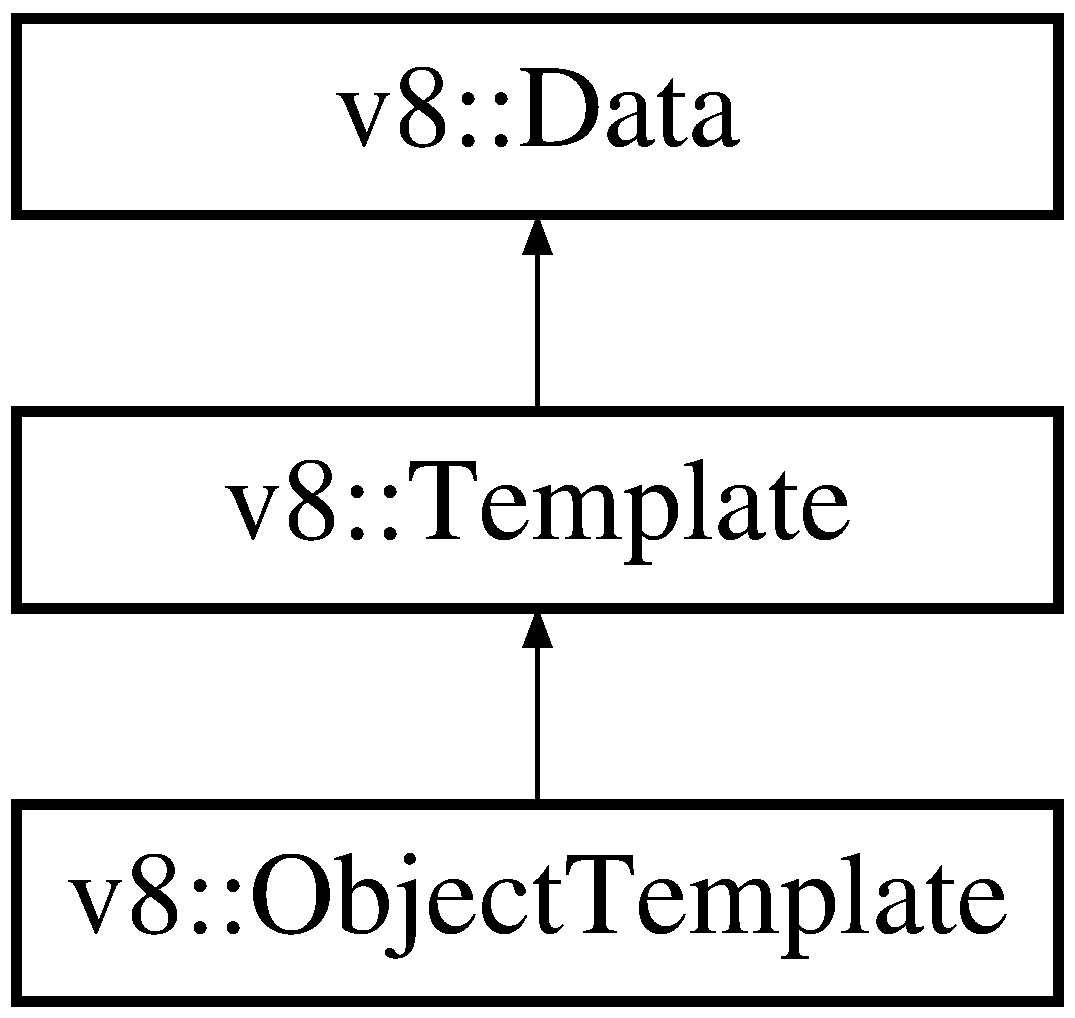
\includegraphics[height=3.000000cm]{classv8_1_1_object_template}
\end{center}
\end{figure}
\subsection*{Public Member Functions}
\begin{DoxyCompactItemize}
\item 
\hyperlink{classv8_1_1_object_template_abfa44addb7c9b426036a34bc7e60cc20}{V8\+\_\+\+D\+E\+P\+R\+E\+C\+A\+T\+E\+\_\+\+S\+O\+ON} (\char`\"{}Use maybe version\char`\"{}, Local$<$ \hyperlink{classv8_1_1_object}{Object} $>$ New\+Instance())
\item 
V8\+\_\+\+W\+A\+R\+N\+\_\+\+U\+N\+U\+S\+E\+D\+\_\+\+R\+E\+S\+U\+LT \hyperlink{classv8_1_1_maybe_local}{Maybe\+Local}$<$ \hyperlink{classv8_1_1_object}{Object} $>$ {\bfseries New\+Instance} (\hyperlink{classv8_1_1_local}{Local}$<$ \hyperlink{classv8_1_1_context}{Context} $>$ context)\hypertarget{classv8_1_1_object_template_a76c118a457f70ec9ec24cf24985655ff}{}\label{classv8_1_1_object_template_a76c118a457f70ec9ec24cf24985655ff}

\item 
void \hyperlink{classv8_1_1_object_template_a7300126e15ff8246813e07f92d4fbe83}{Set\+Accessor} (\hyperlink{classv8_1_1_local}{Local}$<$ \hyperlink{classv8_1_1_string}{String} $>$ name, \hyperlink{namespacev8_a722613c87061708a4f1aa050d095f868}{Accessor\+Getter\+Callback} getter, Accessor\+Setter\+Callback setter=0, \hyperlink{classv8_1_1_local}{Local}$<$ \hyperlink{classv8_1_1_value}{Value} $>$ data=\hyperlink{classv8_1_1_local}{Local}$<$ \hyperlink{classv8_1_1_value}{Value} $>$(), \hyperlink{namespacev8_a31d8355cb043d7d2dda3f4a52760b64e}{Access\+Control} settings=D\+E\+F\+A\+U\+LT, Property\+Attribute attribute=None, \hyperlink{classv8_1_1_local}{Local}$<$ \hyperlink{classv8_1_1_accessor_signature}{Accessor\+Signature} $>$ signature=\hyperlink{classv8_1_1_local}{Local}$<$ \hyperlink{classv8_1_1_accessor_signature}{Accessor\+Signature} $>$())
\item 
void {\bfseries Set\+Accessor} (\hyperlink{classv8_1_1_local}{Local}$<$ \hyperlink{classv8_1_1_name}{Name} $>$ name, Accessor\+Name\+Getter\+Callback getter, Accessor\+Name\+Setter\+Callback setter=0, \hyperlink{classv8_1_1_local}{Local}$<$ \hyperlink{classv8_1_1_value}{Value} $>$ data=\hyperlink{classv8_1_1_local}{Local}$<$ \hyperlink{classv8_1_1_value}{Value} $>$(), \hyperlink{namespacev8_a31d8355cb043d7d2dda3f4a52760b64e}{Access\+Control} settings=D\+E\+F\+A\+U\+LT, Property\+Attribute attribute=None, \hyperlink{classv8_1_1_local}{Local}$<$ \hyperlink{classv8_1_1_accessor_signature}{Accessor\+Signature} $>$ signature=\hyperlink{classv8_1_1_local}{Local}$<$ \hyperlink{classv8_1_1_accessor_signature}{Accessor\+Signature} $>$())\hypertarget{classv8_1_1_object_template_a5efa63efe7659c138645eae226d30f2b}{}\label{classv8_1_1_object_template_a5efa63efe7659c138645eae226d30f2b}

\item 
void \hyperlink{classv8_1_1_object_template_a66fa7b04c87676e20e35497ea09a0ad0}{Set\+Named\+Property\+Handler} (\hyperlink{namespacev8_a50cae386a68bf9ff23d02aa1161face4}{Named\+Property\+Getter\+Callback} getter, \hyperlink{namespacev8_a9587769513971dc7cb301b740d9e66b6}{Named\+Property\+Setter\+Callback} setter=0, \hyperlink{namespacev8_ac135beae5f0c8b290255accb438f990e}{Named\+Property\+Query\+Callback} query=0, \hyperlink{namespacev8_aaba861076c5b111912cfa0791d348437}{Named\+Property\+Deleter\+Callback} deleter=0, \hyperlink{namespacev8_a5f6f16818a9cddacadbfe6d90ca3a6b1}{Named\+Property\+Enumerator\+Callback} enumerator=0, \hyperlink{classv8_1_1_local}{Local}$<$ \hyperlink{classv8_1_1_value}{Value} $>$ data=\hyperlink{classv8_1_1_local}{Local}$<$ \hyperlink{classv8_1_1_value}{Value} $>$())
\item 
void {\bfseries Set\+Handler} (const \hyperlink{structv8_1_1_named_property_handler_configuration}{Named\+Property\+Handler\+Configuration} \&configuration)\hypertarget{classv8_1_1_object_template_a3d5666f1e9b0f46df6b4dbb7cfbb6114}{}\label{classv8_1_1_object_template_a3d5666f1e9b0f46df6b4dbb7cfbb6114}

\item 
void \hyperlink{classv8_1_1_object_template_abc92c2889776a5a1ef6831f9c3da3783}{Set\+Handler} (const \hyperlink{structv8_1_1_indexed_property_handler_configuration}{Indexed\+Property\+Handler\+Configuration} \&configuration)
\item 
void {\bfseries Set\+Indexed\+Property\+Handler} (\hyperlink{namespacev8_a48e7816ba64447bf32a25d194588daaf}{Indexed\+Property\+Getter\+Callback} getter, \hyperlink{namespacev8_a4ac7cc6185ebc8b6a199f9fa8e6bf5c3}{Indexed\+Property\+Setter\+Callback} setter=0, \hyperlink{namespacev8_a980b62c33eb664783e61e25c3b27f9ee}{Indexed\+Property\+Query\+Callback} query=0, \hyperlink{namespacev8_a53863728de14cde48dd6543207b2f2da}{Indexed\+Property\+Deleter\+Callback} deleter=0, \hyperlink{namespacev8_adbb0a6d5537371953f9ba807d4f6275e}{Indexed\+Property\+Enumerator\+Callback} enumerator=0, \hyperlink{classv8_1_1_local}{Local}$<$ \hyperlink{classv8_1_1_value}{Value} $>$ data=\hyperlink{classv8_1_1_local}{Local}$<$ \hyperlink{classv8_1_1_value}{Value} $>$())\hypertarget{classv8_1_1_object_template_ae3303f3d55370684ac02b02e67712eac}{}\label{classv8_1_1_object_template_ae3303f3d55370684ac02b02e67712eac}

\item 
void \hyperlink{classv8_1_1_object_template_a1775c8f73e643c339804d2f5b628eddf}{Set\+Call\+As\+Function\+Handler} (Function\+Callback callback, \hyperlink{classv8_1_1_local}{Local}$<$ \hyperlink{classv8_1_1_value}{Value} $>$ data=\hyperlink{classv8_1_1_local}{Local}$<$ \hyperlink{classv8_1_1_value}{Value} $>$())
\item 
void \hyperlink{classv8_1_1_object_template_a7e40ef313b44c2ad336c73051523b4f8}{Mark\+As\+Undetectable} ()
\item 
void \hyperlink{classv8_1_1_object_template_a5b0337016cd89fc72f3a9d75399c2487}{Set\+Access\+Check\+Callback} (\hyperlink{namespacev8_a1024fb358d107c1494163217830688e6}{Access\+Check\+Callback} callback, \hyperlink{classv8_1_1_local}{Local}$<$ \hyperlink{classv8_1_1_value}{Value} $>$ data=\hyperlink{classv8_1_1_local}{Local}$<$ \hyperlink{classv8_1_1_value}{Value} $>$())
\item 
{\bfseries V8\+\_\+\+D\+E\+P\+R\+E\+C\+A\+T\+ED} (\char`\"{}Use \hyperlink{classv8_1_1_object_template_a5b0337016cd89fc72f3a9d75399c2487}{Set\+Access\+Check\+Callback} with new \hyperlink{namespacev8_a1024fb358d107c1494163217830688e6}{Access\+Check\+Callback} signature.\char`\"{}, void \hyperlink{classv8_1_1_object_template_a5b0337016cd89fc72f3a9d75399c2487}{Set\+Access\+Check\+Callback}(Deprecated\+Access\+Check\+Callback callback,                                                                                                                               \hyperlink{classv8_1_1_local}{Local}$<$ \hyperlink{classv8_1_1_value}{Value} $>$ data=\hyperlink{classv8_1_1_local}{Local}$<$ \hyperlink{classv8_1_1_value}{Value} $>$()))\hypertarget{classv8_1_1_object_template_a816e285cb9f2a23b15bf7a718bc6a7fa}{}\label{classv8_1_1_object_template_a816e285cb9f2a23b15bf7a718bc6a7fa}

\item 
{\bfseries V8\+\_\+\+D\+E\+P\+R\+E\+C\+A\+T\+ED} (\char`\"{}Use \hyperlink{classv8_1_1_object_template_a5b0337016cd89fc72f3a9d75399c2487}{Set\+Access\+Check\+Callback} instead\char`\"{}, void Set\+Access\+Check\+Callbacks(\hyperlink{namespacev8_ab5cafda0c556bba990c660ce9c904e0d}{Named\+Security\+Callback} named\+\_\+handler,                                                                                                                                   \hyperlink{namespacev8_aebbcc7837753e51112d944ad96520da1}{Indexed\+Security\+Callback} indexed\+\_\+handler,                                                                                                                                   \hyperlink{classv8_1_1_local}{Local}$<$ \hyperlink{classv8_1_1_value}{Value} $>$ data=\hyperlink{classv8_1_1_local}{Local}$<$ \hyperlink{classv8_1_1_value}{Value} $>$()))\hypertarget{classv8_1_1_object_template_a1b3293962bb1685f127a58ab3ef3d29d}{}\label{classv8_1_1_object_template_a1b3293962bb1685f127a58ab3ef3d29d}

\item 
int \hyperlink{classv8_1_1_object_template_a43de785d594d8c01b18230b1aa79e31c}{Internal\+Field\+Count} ()
\item 
void \hyperlink{classv8_1_1_object_template_ab63916ac584a76bca8ba541f86ce9fce}{Set\+Internal\+Field\+Count} (int value)
\end{DoxyCompactItemize}
\subsection*{Static Public Member Functions}
\begin{DoxyCompactItemize}
\item 
static \hyperlink{classv8_1_1_local}{Local}$<$ \hyperlink{classv8_1_1_object_template}{Object\+Template} $>$ \hyperlink{classv8_1_1_object_template_a092e8adf656359d4dead412d28313ebb}{New} (\hyperlink{classv8_1_1_isolate}{Isolate} $\ast$isolate, \hyperlink{classv8_1_1_local}{Local}$<$ \hyperlink{classv8_1_1_function_template}{Function\+Template} $>$ constructor=\hyperlink{classv8_1_1_local}{Local}$<$ \hyperlink{classv8_1_1_function_template}{Function\+Template} $>$())
\item 
static {\bfseries V8\+\_\+\+D\+E\+P\+R\+E\+C\+A\+T\+ED} (\char`\"{}Use isolate version\char`\"{}, Local$<$ \hyperlink{classv8_1_1_object_template}{Object\+Template} $>$ \hyperlink{classv8_1_1_object_template_a092e8adf656359d4dead412d28313ebb}{New}())\hypertarget{classv8_1_1_object_template_aca569a9eafe2f49f8638e0157d1b20a2}{}\label{classv8_1_1_object_template_aca569a9eafe2f49f8638e0157d1b20a2}

\end{DoxyCompactItemize}
\subsection*{Static Private Member Functions}
\begin{DoxyCompactItemize}
\item 
static \hyperlink{classv8_1_1_local}{Local}$<$ \hyperlink{classv8_1_1_object_template}{Object\+Template} $>$ {\bfseries New} (\hyperlink{classv8_1_1internal_1_1_isolate}{internal\+::\+Isolate} $\ast$isolate, \hyperlink{classv8_1_1_local}{Local}$<$ \hyperlink{classv8_1_1_function_template}{Function\+Template} $>$ constructor)\hypertarget{classv8_1_1_object_template_a16d886ee105d6ede4b560831f0160d31}{}\label{classv8_1_1_object_template_a16d886ee105d6ede4b560831f0160d31}

\end{DoxyCompactItemize}
\subsection*{Friends}
\begin{DoxyCompactItemize}
\item 
class {\bfseries Function\+Template}\hypertarget{classv8_1_1_object_template_a334168ad1a5f39cf17b818ca3356aacd}{}\label{classv8_1_1_object_template_a334168ad1a5f39cf17b818ca3356aacd}

\end{DoxyCompactItemize}


\subsection{Detailed Description}
An \hyperlink{classv8_1_1_object_template}{Object\+Template} is used to create objects at runtime.

Properties added to an \hyperlink{classv8_1_1_object_template}{Object\+Template} are added to each object created from the \hyperlink{classv8_1_1_object_template}{Object\+Template}. 

\subsection{Member Function Documentation}
\index{v8\+::\+Object\+Template@{v8\+::\+Object\+Template}!Internal\+Field\+Count@{Internal\+Field\+Count}}
\index{Internal\+Field\+Count@{Internal\+Field\+Count}!v8\+::\+Object\+Template@{v8\+::\+Object\+Template}}
\subsubsection[{\texorpdfstring{Internal\+Field\+Count()}{InternalFieldCount()}}]{\setlength{\rightskip}{0pt plus 5cm}int v8\+::\+Object\+Template\+::\+Internal\+Field\+Count (
\begin{DoxyParamCaption}
{}
\end{DoxyParamCaption}
)}\hypertarget{classv8_1_1_object_template_a43de785d594d8c01b18230b1aa79e31c}{}\label{classv8_1_1_object_template_a43de785d594d8c01b18230b1aa79e31c}
Gets the number of internal fields for objects generated from this template. \index{v8\+::\+Object\+Template@{v8\+::\+Object\+Template}!Mark\+As\+Undetectable@{Mark\+As\+Undetectable}}
\index{Mark\+As\+Undetectable@{Mark\+As\+Undetectable}!v8\+::\+Object\+Template@{v8\+::\+Object\+Template}}
\subsubsection[{\texorpdfstring{Mark\+As\+Undetectable()}{MarkAsUndetectable()}}]{\setlength{\rightskip}{0pt plus 5cm}void v8\+::\+Object\+Template\+::\+Mark\+As\+Undetectable (
\begin{DoxyParamCaption}
{}
\end{DoxyParamCaption}
)}\hypertarget{classv8_1_1_object_template_a7e40ef313b44c2ad336c73051523b4f8}{}\label{classv8_1_1_object_template_a7e40ef313b44c2ad336c73051523b4f8}
Mark object instances of the template as undetectable.

In many ways, undetectable objects behave as though they are not there. They behave like \textquotesingle{}undefined\textquotesingle{} in conditionals and when printed. However, properties can be accessed and called as on normal objects. \index{v8\+::\+Object\+Template@{v8\+::\+Object\+Template}!New@{New}}
\index{New@{New}!v8\+::\+Object\+Template@{v8\+::\+Object\+Template}}
\subsubsection[{\texorpdfstring{New(\+Isolate $\ast$isolate, Local$<$ Function\+Template $>$ constructor=\+Local$<$ Function\+Template $>$())}{New(Isolate *isolate, Local< FunctionTemplate > constructor=Local< FunctionTemplate >())}}]{\setlength{\rightskip}{0pt plus 5cm}{\bf Local}$<$ {\bf Object\+Template} $>$ v8\+::\+Object\+Template\+::\+New (
\begin{DoxyParamCaption}
\item[{{\bf Isolate} $\ast$}]{isolate, }
\item[{{\bf v8\+::\+Local}$<$ {\bf Function\+Template} $>$}]{constructor = {\ttfamily {\bf Local}$<${\bf Function\+Template}$>$()}}
\end{DoxyParamCaption}
)\hspace{0.3cm}{\ttfamily [static]}}\hypertarget{classv8_1_1_object_template_a092e8adf656359d4dead412d28313ebb}{}\label{classv8_1_1_object_template_a092e8adf656359d4dead412d28313ebb}
Creates an \hyperlink{classv8_1_1_object_template}{Object\+Template}. \index{v8\+::\+Object\+Template@{v8\+::\+Object\+Template}!Set\+Access\+Check\+Callback@{Set\+Access\+Check\+Callback}}
\index{Set\+Access\+Check\+Callback@{Set\+Access\+Check\+Callback}!v8\+::\+Object\+Template@{v8\+::\+Object\+Template}}
\subsubsection[{\texorpdfstring{Set\+Access\+Check\+Callback(\+Access\+Check\+Callback callback, Local$<$ Value $>$ data=\+Local$<$ Value $>$())}{SetAccessCheckCallback(AccessCheckCallback callback, Local< Value > data=Local< Value >())}}]{\setlength{\rightskip}{0pt plus 5cm}void v8\+::\+Object\+Template\+::\+Set\+Access\+Check\+Callback (
\begin{DoxyParamCaption}
\item[{{\bf Access\+Check\+Callback}}]{callback, }
\item[{{\bf Local}$<$ {\bf Value} $>$}]{data = {\ttfamily {\bf Local}$<${\bf Value}$>$()}}
\end{DoxyParamCaption}
)}\hypertarget{classv8_1_1_object_template_a5b0337016cd89fc72f3a9d75399c2487}{}\label{classv8_1_1_object_template_a5b0337016cd89fc72f3a9d75399c2487}
Sets access check callback on the object template and enables access checks.

When accessing properties on instances of this object template, the access check callback will be called to determine whether or not to allow cross-\/context access to the properties. \index{v8\+::\+Object\+Template@{v8\+::\+Object\+Template}!Set\+Accessor@{Set\+Accessor}}
\index{Set\+Accessor@{Set\+Accessor}!v8\+::\+Object\+Template@{v8\+::\+Object\+Template}}
\subsubsection[{\texorpdfstring{Set\+Accessor(\+Local$<$ String $>$ name, Accessor\+Getter\+Callback getter, Accessor\+Setter\+Callback setter=0, Local$<$ Value $>$ data=\+Local$<$ Value $>$(), Access\+Control settings=\+D\+E\+F\+A\+U\+L\+T, Property\+Attribute attribute=\+None, Local$<$ Accessor\+Signature $>$ signature=\+Local$<$ Accessor\+Signature $>$())}{SetAccessor(Local< String > name, AccessorGetterCallback getter, AccessorSetterCallback setter=0, Local< Value > data=Local< Value >(), AccessControl settings=DEFAULT, PropertyAttribute attribute=None, Local< AccessorSignature > signature=Local< AccessorSignature >())}}]{\setlength{\rightskip}{0pt plus 5cm}void v8\+::\+Object\+Template\+::\+Set\+Accessor (
\begin{DoxyParamCaption}
\item[{{\bf v8\+::\+Local}$<$ {\bf String} $>$}]{name, }
\item[{{\bf Accessor\+Getter\+Callback}}]{getter, }
\item[{Accessor\+Setter\+Callback}]{setter = {\ttfamily 0}, }
\item[{{\bf v8\+::\+Local}$<$ {\bf Value} $>$}]{data = {\ttfamily {\bf Local}$<${\bf Value}$>$()}, }
\item[{{\bf Access\+Control}}]{settings = {\ttfamily DEFAULT}, }
\item[{Property\+Attribute}]{attribute = {\ttfamily None}, }
\item[{{\bf v8\+::\+Local}$<$ {\bf Accessor\+Signature} $>$}]{signature = {\ttfamily {\bf Local}$<${\bf Accessor\+Signature}$>$()}}
\end{DoxyParamCaption}
)}\hypertarget{classv8_1_1_object_template_a7300126e15ff8246813e07f92d4fbe83}{}\label{classv8_1_1_object_template_a7300126e15ff8246813e07f92d4fbe83}
Sets an accessor on the object template.

Whenever the property with the given name is accessed on objects created from this \hyperlink{classv8_1_1_object_template}{Object\+Template} the getter and setter callbacks are called instead of getting and setting the property directly on the Java\+Script object.


\begin{DoxyParams}{Parameters}
{\em name} & The name of the property for which an accessor is added. \\
\hline
{\em getter} & The callback to invoke when getting the property. \\
\hline
{\em setter} & The callback to invoke when setting the property. \\
\hline
{\em data} & A piece of data that will be passed to the getter and setter callbacks whenever they are invoked. \\
\hline
{\em settings} & Access control settings for the accessor. This is a bit field consisting of one of more of D\+E\+F\+A\+U\+LT = 0, A\+L\+L\+\_\+\+C\+A\+N\+\_\+\+R\+E\+AD = 1, or A\+L\+L\+\_\+\+C\+A\+N\+\_\+\+W\+R\+I\+TE = 2. The default is to not allow cross-\/context access. A\+L\+L\+\_\+\+C\+A\+N\+\_\+\+R\+E\+AD means that all cross-\/context reads are allowed. A\+L\+L\+\_\+\+C\+A\+N\+\_\+\+W\+R\+I\+TE means that all cross-\/context writes are allowed. The combination A\+L\+L\+\_\+\+C\+A\+N\+\_\+\+R\+E\+AD $\vert$ A\+L\+L\+\_\+\+C\+A\+N\+\_\+\+W\+R\+I\+TE can be used to allow all cross-\/context access. \\
\hline
{\em attribute} & The attributes of the property for which an accessor is added. \\
\hline
{\em signature} & The signature describes valid receivers for the accessor and is used to perform implicit instance checks against them. If the receiver is incompatible (i.\+e. is not an instance of the constructor as defined by \hyperlink{classv8_1_1_function_template_a90d838f3456d300bd19d2a2cb98645bd}{Function\+Template\+::\+Has\+Instance()}), an implicit Type\+Error is thrown and no callback is invoked. \\
\hline
\end{DoxyParams}
\index{v8\+::\+Object\+Template@{v8\+::\+Object\+Template}!Set\+Call\+As\+Function\+Handler@{Set\+Call\+As\+Function\+Handler}}
\index{Set\+Call\+As\+Function\+Handler@{Set\+Call\+As\+Function\+Handler}!v8\+::\+Object\+Template@{v8\+::\+Object\+Template}}
\subsubsection[{\texorpdfstring{Set\+Call\+As\+Function\+Handler(\+Function\+Callback callback, Local$<$ Value $>$ data=\+Local$<$ Value $>$())}{SetCallAsFunctionHandler(FunctionCallback callback, Local< Value > data=Local< Value >())}}]{\setlength{\rightskip}{0pt plus 5cm}void v8\+::\+Object\+Template\+::\+Set\+Call\+As\+Function\+Handler (
\begin{DoxyParamCaption}
\item[{Function\+Callback}]{callback, }
\item[{{\bf Local}$<$ {\bf Value} $>$}]{data = {\ttfamily {\bf Local}$<${\bf Value}$>$()}}
\end{DoxyParamCaption}
)}\hypertarget{classv8_1_1_object_template_a1775c8f73e643c339804d2f5b628eddf}{}\label{classv8_1_1_object_template_a1775c8f73e643c339804d2f5b628eddf}
Sets the callback to be used when calling instances created from this template as a function. If no callback is set, instances behave like normal Java\+Script objects that cannot be called as a function. \index{v8\+::\+Object\+Template@{v8\+::\+Object\+Template}!Set\+Handler@{Set\+Handler}}
\index{Set\+Handler@{Set\+Handler}!v8\+::\+Object\+Template@{v8\+::\+Object\+Template}}
\subsubsection[{\texorpdfstring{Set\+Handler(const Indexed\+Property\+Handler\+Configuration \&configuration)}{SetHandler(const IndexedPropertyHandlerConfiguration &configuration)}}]{\setlength{\rightskip}{0pt plus 5cm}void v8\+::\+Object\+Template\+::\+Set\+Handler (
\begin{DoxyParamCaption}
\item[{const {\bf Indexed\+Property\+Handler\+Configuration} \&}]{configuration}
\end{DoxyParamCaption}
)}\hypertarget{classv8_1_1_object_template_abc92c2889776a5a1ef6831f9c3da3783}{}\label{classv8_1_1_object_template_abc92c2889776a5a1ef6831f9c3da3783}
Sets an indexed property handler on the object template.

Whenever an indexed property is accessed on objects created from this object template, the provided callback is invoked instead of accessing the property directly on the Java\+Script object.


\begin{DoxyParams}{Parameters}
{\em getter} & The callback to invoke when getting a property. \\
\hline
{\em setter} & The callback to invoke when setting a property. \\
\hline
{\em query} & The callback to invoke to check if an object has a property. \\
\hline
{\em deleter} & The callback to invoke when deleting a property. \\
\hline
{\em enumerator} & The callback to invoke to enumerate all the indexed properties of an object. \\
\hline
{\em data} & A piece of data that will be passed to the callbacks whenever they are invoked. \\
\hline
\end{DoxyParams}
\index{v8\+::\+Object\+Template@{v8\+::\+Object\+Template}!Set\+Internal\+Field\+Count@{Set\+Internal\+Field\+Count}}
\index{Set\+Internal\+Field\+Count@{Set\+Internal\+Field\+Count}!v8\+::\+Object\+Template@{v8\+::\+Object\+Template}}
\subsubsection[{\texorpdfstring{Set\+Internal\+Field\+Count(int value)}{SetInternalFieldCount(int value)}}]{\setlength{\rightskip}{0pt plus 5cm}void v8\+::\+Object\+Template\+::\+Set\+Internal\+Field\+Count (
\begin{DoxyParamCaption}
\item[{int}]{value}
\end{DoxyParamCaption}
)}\hypertarget{classv8_1_1_object_template_ab63916ac584a76bca8ba541f86ce9fce}{}\label{classv8_1_1_object_template_ab63916ac584a76bca8ba541f86ce9fce}
Sets the number of internal fields for objects generated from this template. \index{v8\+::\+Object\+Template@{v8\+::\+Object\+Template}!Set\+Named\+Property\+Handler@{Set\+Named\+Property\+Handler}}
\index{Set\+Named\+Property\+Handler@{Set\+Named\+Property\+Handler}!v8\+::\+Object\+Template@{v8\+::\+Object\+Template}}
\subsubsection[{\texorpdfstring{Set\+Named\+Property\+Handler(\+Named\+Property\+Getter\+Callback getter, Named\+Property\+Setter\+Callback setter=0, Named\+Property\+Query\+Callback query=0, Named\+Property\+Deleter\+Callback deleter=0, Named\+Property\+Enumerator\+Callback enumerator=0, Local$<$ Value $>$ data=\+Local$<$ Value $>$())}{SetNamedPropertyHandler(NamedPropertyGetterCallback getter, NamedPropertySetterCallback setter=0, NamedPropertyQueryCallback query=0, NamedPropertyDeleterCallback deleter=0, NamedPropertyEnumeratorCallback enumerator=0, Local< Value > data=Local< Value >())}}]{\setlength{\rightskip}{0pt plus 5cm}void v8\+::\+Object\+Template\+::\+Set\+Named\+Property\+Handler (
\begin{DoxyParamCaption}
\item[{{\bf Named\+Property\+Getter\+Callback}}]{getter, }
\item[{{\bf Named\+Property\+Setter\+Callback}}]{setter = {\ttfamily 0}, }
\item[{{\bf Named\+Property\+Query\+Callback}}]{query = {\ttfamily 0}, }
\item[{{\bf Named\+Property\+Deleter\+Callback}}]{deleter = {\ttfamily 0}, }
\item[{{\bf Named\+Property\+Enumerator\+Callback}}]{enumerator = {\ttfamily 0}, }
\item[{{\bf Local}$<$ {\bf Value} $>$}]{data = {\ttfamily {\bf Local}$<${\bf Value}$>$()}}
\end{DoxyParamCaption}
)}\hypertarget{classv8_1_1_object_template_a66fa7b04c87676e20e35497ea09a0ad0}{}\label{classv8_1_1_object_template_a66fa7b04c87676e20e35497ea09a0ad0}
Sets a named property handler on the object template.

Whenever a property whose name is a string is accessed on objects created from this object template, the provided callback is invoked instead of accessing the property directly on the Java\+Script object.

Note that new code should use the second version that can intercept symbol-\/named properties as well as string-\/named properties.


\begin{DoxyParams}{Parameters}
{\em getter} & The callback to invoke when getting a property. \\
\hline
{\em setter} & The callback to invoke when setting a property. \\
\hline
{\em query} & The callback to invoke to check if a property is present, and if present, get its attributes. \\
\hline
{\em deleter} & The callback to invoke when deleting a property. \\
\hline
{\em enumerator} & The callback to invoke to enumerate all the named properties of an object. \\
\hline
{\em data} & A piece of data that will be passed to the callbacks whenever they are invoked. \\
\hline
\end{DoxyParams}
\index{v8\+::\+Object\+Template@{v8\+::\+Object\+Template}!V8\+\_\+\+D\+E\+P\+R\+E\+C\+A\+T\+E\+\_\+\+S\+O\+ON@{V8\+\_\+\+D\+E\+P\+R\+E\+C\+A\+T\+E\+\_\+\+S\+O\+ON}}
\index{V8\+\_\+\+D\+E\+P\+R\+E\+C\+A\+T\+E\+\_\+\+S\+O\+ON@{V8\+\_\+\+D\+E\+P\+R\+E\+C\+A\+T\+E\+\_\+\+S\+O\+ON}!v8\+::\+Object\+Template@{v8\+::\+Object\+Template}}
\subsubsection[{\texorpdfstring{V8\+\_\+\+D\+E\+P\+R\+E\+C\+A\+T\+E\+\_\+\+S\+O\+O\+N(""Use maybe version"", Local$<$ Object $>$ New\+Instance())}{V8_DEPRECATE_SOON("Use maybe version", Local< Object > NewInstance())}}]{\setlength{\rightskip}{0pt plus 5cm}v8\+::\+Object\+Template\+::\+V8\+\_\+\+D\+E\+P\+R\+E\+C\+A\+T\+E\+\_\+\+S\+O\+ON (
\begin{DoxyParamCaption}
\item[{\char`\"{}Use maybe version\char`\"{}}]{, }
\item[{{\bf Local}$<$ {\bf Object} $>$ }]{New\+Instance()}
\end{DoxyParamCaption}
)}\hypertarget{classv8_1_1_object_template_abfa44addb7c9b426036a34bc7e60cc20}{}\label{classv8_1_1_object_template_abfa44addb7c9b426036a34bc7e60cc20}
Creates a new instance of this template. 

The documentation for this class was generated from the following files\+:\begin{DoxyCompactItemize}
\item 
/\+Users/joshgav/node/v8/include/v8.\+h\item 
/\+Users/joshgav/node/v8/src/api.\+cc\end{DoxyCompactItemize}

\hypertarget{classv8_1_1_output_stream}{}\section{v8\+:\+:Output\+Stream Class Reference}
\label{classv8_1_1_output_stream}\index{v8\+::\+Output\+Stream@{v8\+::\+Output\+Stream}}


{\ttfamily \#include $<$v8-\/profiler.\+h$>$}

\subsection*{Public Types}
\begin{DoxyCompactItemize}
\item 
enum {\bfseries Write\+Result} \{ \\*
{\bfseries k\+Continue} = 0, 
\\*
{\bfseries k\+Abort} = 1
 \}\hypertarget{classv8_1_1_output_stream_a336c7605a0ce4fbe6f6fca3b03bc16de}{}\label{classv8_1_1_output_stream_a336c7605a0ce4fbe6f6fca3b03bc16de}

\end{DoxyCompactItemize}
\subsection*{Public Member Functions}
\begin{DoxyCompactItemize}
\item 
virtual void \hyperlink{classv8_1_1_output_stream_a6c5c308367fc5776bcbedff0e94d6049}{End\+Of\+Stream} ()=0
\item 
virtual int \hyperlink{classv8_1_1_output_stream_a93bdaa790cbd66a7283fad2cca3f48f7}{Get\+Chunk\+Size} ()
\item 
virtual Write\+Result \hyperlink{classv8_1_1_output_stream_a42adc62ebe43d00159f80328538f217f}{Write\+Ascii\+Chunk} (char $\ast$data, int size)=0
\item 
virtual Write\+Result \hyperlink{classv8_1_1_output_stream_a104fd1a0b5ef685e1d4967aaacbb9e9d}{Write\+Heap\+Stats\+Chunk} (\hyperlink{structv8_1_1_heap_stats_update}{Heap\+Stats\+Update} $\ast$data, int count)
\end{DoxyCompactItemize}


\subsection{Detailed Description}
An interface for exporting data from \hyperlink{classv8_1_1_v8}{V8}, using \char`\"{}push\char`\"{} model. 

\subsection{Member Function Documentation}
\index{v8\+::\+Output\+Stream@{v8\+::\+Output\+Stream}!End\+Of\+Stream@{End\+Of\+Stream}}
\index{End\+Of\+Stream@{End\+Of\+Stream}!v8\+::\+Output\+Stream@{v8\+::\+Output\+Stream}}
\subsubsection[{\texorpdfstring{End\+Of\+Stream()=0}{EndOfStream()=0}}]{\setlength{\rightskip}{0pt plus 5cm}virtual void v8\+::\+Output\+Stream\+::\+End\+Of\+Stream (
\begin{DoxyParamCaption}
{}
\end{DoxyParamCaption}
)\hspace{0.3cm}{\ttfamily [pure virtual]}}\hypertarget{classv8_1_1_output_stream_a6c5c308367fc5776bcbedff0e94d6049}{}\label{classv8_1_1_output_stream_a6c5c308367fc5776bcbedff0e94d6049}
Notify about the end of stream. \index{v8\+::\+Output\+Stream@{v8\+::\+Output\+Stream}!Get\+Chunk\+Size@{Get\+Chunk\+Size}}
\index{Get\+Chunk\+Size@{Get\+Chunk\+Size}!v8\+::\+Output\+Stream@{v8\+::\+Output\+Stream}}
\subsubsection[{\texorpdfstring{Get\+Chunk\+Size()}{GetChunkSize()}}]{\setlength{\rightskip}{0pt plus 5cm}virtual int v8\+::\+Output\+Stream\+::\+Get\+Chunk\+Size (
\begin{DoxyParamCaption}
{}
\end{DoxyParamCaption}
)\hspace{0.3cm}{\ttfamily [inline]}, {\ttfamily [virtual]}}\hypertarget{classv8_1_1_output_stream_a93bdaa790cbd66a7283fad2cca3f48f7}{}\label{classv8_1_1_output_stream_a93bdaa790cbd66a7283fad2cca3f48f7}
Get preferred output chunk size. Called only once. \index{v8\+::\+Output\+Stream@{v8\+::\+Output\+Stream}!Write\+Ascii\+Chunk@{Write\+Ascii\+Chunk}}
\index{Write\+Ascii\+Chunk@{Write\+Ascii\+Chunk}!v8\+::\+Output\+Stream@{v8\+::\+Output\+Stream}}
\subsubsection[{\texorpdfstring{Write\+Ascii\+Chunk(char $\ast$data, int size)=0}{WriteAsciiChunk(char *data, int size)=0}}]{\setlength{\rightskip}{0pt plus 5cm}virtual Write\+Result v8\+::\+Output\+Stream\+::\+Write\+Ascii\+Chunk (
\begin{DoxyParamCaption}
\item[{char $\ast$}]{data, }
\item[{int}]{size}
\end{DoxyParamCaption}
)\hspace{0.3cm}{\ttfamily [pure virtual]}}\hypertarget{classv8_1_1_output_stream_a42adc62ebe43d00159f80328538f217f}{}\label{classv8_1_1_output_stream_a42adc62ebe43d00159f80328538f217f}
Writes the next chunk of snapshot data into the stream. Writing can be stopped by returning k\+Abort as function result. End\+Of\+Stream will not be called in case writing was aborted. \index{v8\+::\+Output\+Stream@{v8\+::\+Output\+Stream}!Write\+Heap\+Stats\+Chunk@{Write\+Heap\+Stats\+Chunk}}
\index{Write\+Heap\+Stats\+Chunk@{Write\+Heap\+Stats\+Chunk}!v8\+::\+Output\+Stream@{v8\+::\+Output\+Stream}}
\subsubsection[{\texorpdfstring{Write\+Heap\+Stats\+Chunk(\+Heap\+Stats\+Update $\ast$data, int count)}{WriteHeapStatsChunk(HeapStatsUpdate *data, int count)}}]{\setlength{\rightskip}{0pt plus 5cm}virtual Write\+Result v8\+::\+Output\+Stream\+::\+Write\+Heap\+Stats\+Chunk (
\begin{DoxyParamCaption}
\item[{{\bf Heap\+Stats\+Update} $\ast$}]{data, }
\item[{int}]{count}
\end{DoxyParamCaption}
)\hspace{0.3cm}{\ttfamily [inline]}, {\ttfamily [virtual]}}\hypertarget{classv8_1_1_output_stream_a104fd1a0b5ef685e1d4967aaacbb9e9d}{}\label{classv8_1_1_output_stream_a104fd1a0b5ef685e1d4967aaacbb9e9d}
Writes the next chunk of heap stats data into the stream. Writing can be stopped by returning k\+Abort as function result. End\+Of\+Stream will not be called in case writing was aborted. 

The documentation for this class was generated from the following file\+:\begin{DoxyCompactItemize}
\item 
/\+Users/joshgav/node/v8/include/v8-\/profiler.\+h\end{DoxyCompactItemize}

\hypertarget{classv8_1_1_persistent}{}\section{v8\+:\+:Persistent$<$ T, M $>$ Class Template Reference}
\label{classv8_1_1_persistent}\index{v8\+::\+Persistent$<$ T, M $>$@{v8\+::\+Persistent$<$ T, M $>$}}


{\ttfamily \#include $<$v8.\+h$>$}

Inheritance diagram for v8\+:\+:Persistent$<$ T, M $>$\+:\begin{figure}[H]
\begin{center}
\leavevmode
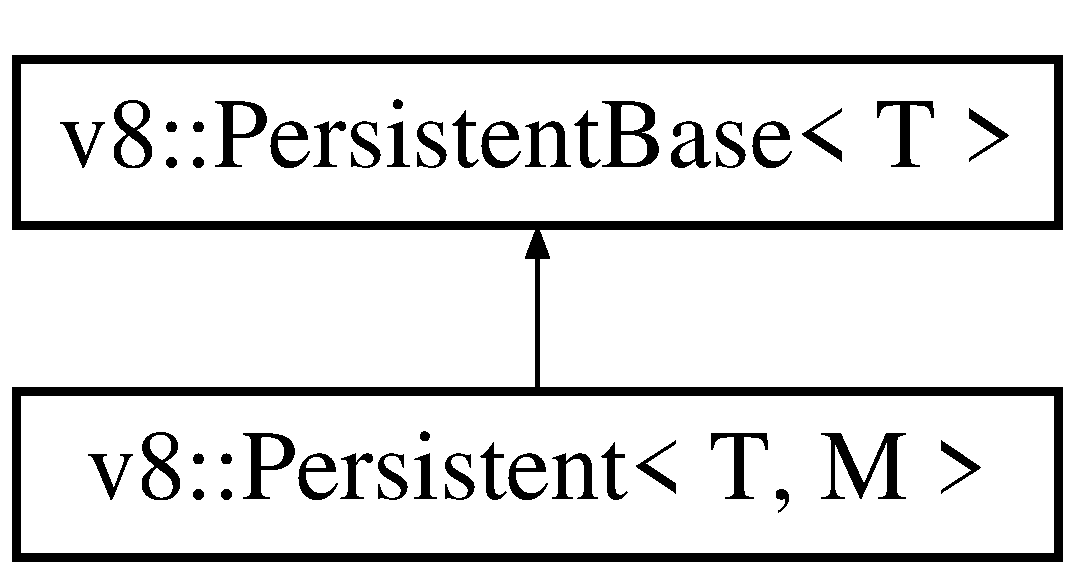
\includegraphics[height=2.000000cm]{classv8_1_1_persistent}
\end{center}
\end{figure}
\subsection*{Public Member Functions}
\begin{DoxyCompactItemize}
\item 
V8\+\_\+\+I\+N\+L\+I\+NE \hyperlink{classv8_1_1_persistent_a5ce14612215393683d814056015a102d}{Persistent} ()
\item 
{\footnotesize template$<$class S $>$ }\\V8\+\_\+\+I\+N\+L\+I\+NE \hyperlink{classv8_1_1_persistent_aabe9a42d7971bd31173bca34186d9ac2}{Persistent} (\hyperlink{classv8_1_1_isolate}{Isolate} $\ast$isolate, \hyperlink{classv8_1_1_local}{Local}$<$ S $>$ that)
\item 
{\footnotesize template$<$class S , class M2 $>$ }\\V8\+\_\+\+I\+N\+L\+I\+NE \hyperlink{classv8_1_1_persistent_aaf9eb7c4e6d0ef2c81a2c08238653578}{Persistent} (\hyperlink{classv8_1_1_isolate}{Isolate} $\ast$isolate, const \hyperlink{classv8_1_1_persistent}{Persistent}$<$ S, M2 $>$ \&that)
\item 
V8\+\_\+\+I\+N\+L\+I\+NE \hyperlink{classv8_1_1_persistent_a22331e91572784cd5ed5519739bb50c7}{Persistent} (const \hyperlink{classv8_1_1_persistent}{Persistent} \&that)
\item 
{\footnotesize template$<$class S , class M2 $>$ }\\V8\+\_\+\+I\+N\+L\+I\+NE {\bfseries Persistent} (const \hyperlink{classv8_1_1_persistent}{Persistent}$<$ S, M2 $>$ \&that)\hypertarget{classv8_1_1_persistent_ace17fd143fb6414d305871bf0a53ef57}{}\label{classv8_1_1_persistent_ace17fd143fb6414d305871bf0a53ef57}

\item 
V8\+\_\+\+I\+N\+L\+I\+NE \hyperlink{classv8_1_1_persistent}{Persistent} \& {\bfseries operator=} (const \hyperlink{classv8_1_1_persistent}{Persistent} \&that)\hypertarget{classv8_1_1_persistent_aa1db9923b3212fb8ce57868217858b39}{}\label{classv8_1_1_persistent_aa1db9923b3212fb8ce57868217858b39}

\item 
{\footnotesize template$<$class S , class M2 $>$ }\\V8\+\_\+\+I\+N\+L\+I\+NE \hyperlink{classv8_1_1_persistent}{Persistent} \& {\bfseries operator=} (const \hyperlink{classv8_1_1_persistent}{Persistent}$<$ S, M2 $>$ \&that)\hypertarget{classv8_1_1_persistent_a11104ee8739cb1f25e40fd17d746b48f}{}\label{classv8_1_1_persistent_a11104ee8739cb1f25e40fd17d746b48f}

\item 
V8\+\_\+\+I\+N\+L\+I\+NE \hyperlink{classv8_1_1_persistent_a7d4d2bebfe3919e447e22adc15464e25}{$\sim$\+Persistent} ()
\item 
{\footnotesize template$<$class S $>$ }\\V8\+\_\+\+I\+N\+L\+I\+NE \hyperlink{classv8_1_1_persistent}{Persistent}$<$ S $>$ \& {\bfseries As} ()\hypertarget{classv8_1_1_persistent_a8d2c96e559ac88f6201d98cb2a626808}{}\label{classv8_1_1_persistent_a8d2c96e559ac88f6201d98cb2a626808}

\item 
{\footnotesize template$<$class S , class M2 $>$ }\\void {\bfseries Copy} (const \hyperlink{classv8_1_1_persistent}{Persistent}$<$ S, M2 $>$ \&that)\hypertarget{classv8_1_1_persistent_ace50a178e3b772f75611e22e41fae974}{}\label{classv8_1_1_persistent_ace50a178e3b772f75611e22e41fae974}

\end{DoxyCompactItemize}
\subsection*{Static Public Member Functions}
\begin{DoxyCompactItemize}
\item 
{\footnotesize template$<$class S $>$ }\\static V8\+\_\+\+I\+N\+L\+I\+NE \hyperlink{classv8_1_1_persistent}{Persistent}$<$ T $>$ \& {\bfseries Cast} (\hyperlink{classv8_1_1_persistent}{Persistent}$<$ S $>$ \&that)\hypertarget{classv8_1_1_persistent_aa20fd9af0b410df9e887689ef97c28dd}{}\label{classv8_1_1_persistent_aa20fd9af0b410df9e887689ef97c28dd}

\end{DoxyCompactItemize}
\subsection*{Private Member Functions}
\begin{DoxyCompactItemize}
\item 
V8\+\_\+\+I\+N\+L\+I\+NE {\bfseries Persistent} (T $\ast$that)\hypertarget{classv8_1_1_persistent_a36492cc837502c9c82ba12a72bf5fb49}{}\label{classv8_1_1_persistent_a36492cc837502c9c82ba12a72bf5fb49}

\item 
V8\+\_\+\+I\+N\+L\+I\+NE T $\ast$ {\bfseries operator$\ast$} () const \hypertarget{classv8_1_1_persistent_a4772ffaf92f953c74b4cb2b3a6dc2c39}{}\label{classv8_1_1_persistent_a4772ffaf92f953c74b4cb2b3a6dc2c39}

\item 
{\footnotesize template$<$class S , class M2 $>$ }\\V8\+\_\+\+I\+N\+L\+I\+NE void {\bfseries Copy} (const \hyperlink{classv8_1_1_persistent}{Persistent}$<$ S, M2 $>$ \&that)\hypertarget{classv8_1_1_persistent_a23a4e84d5d013303896928d52d251283}{}\label{classv8_1_1_persistent_a23a4e84d5d013303896928d52d251283}

\end{DoxyCompactItemize}
\subsection*{Friends}
\begin{DoxyCompactItemize}
\item 
class {\bfseries Isolate}\hypertarget{classv8_1_1_persistent_aba4f0964bdacf2bbf62cf876e5d28d0a}{}\label{classv8_1_1_persistent_aba4f0964bdacf2bbf62cf876e5d28d0a}

\item 
class {\bfseries Utils}\hypertarget{classv8_1_1_persistent_abc0f7da619e9e72510dc07ed7b5ff6d8}{}\label{classv8_1_1_persistent_abc0f7da619e9e72510dc07ed7b5ff6d8}

\item 
{\footnotesize template$<$class F $>$ }\\class {\bfseries Local}\hypertarget{classv8_1_1_persistent_afb872edb4aac7ba55f0da004113aa2b0}{}\label{classv8_1_1_persistent_afb872edb4aac7ba55f0da004113aa2b0}

\item 
{\footnotesize template$<$class F1 , class F2 $>$ }\\class {\bfseries Persistent}\hypertarget{classv8_1_1_persistent_ad845ec8872174be0a9ca9a3dd1898d30}{}\label{classv8_1_1_persistent_ad845ec8872174be0a9ca9a3dd1898d30}

\item 
{\footnotesize template$<$class F $>$ }\\class {\bfseries Return\+Value}\hypertarget{classv8_1_1_persistent_a53f604d3d6f2dc0647df33c9979f116a}{}\label{classv8_1_1_persistent_a53f604d3d6f2dc0647df33c9979f116a}

\end{DoxyCompactItemize}


\subsection{Detailed Description}
\subsubsection*{template$<$class T, class M$>$\\*
class v8\+::\+Persistent$<$ T, M $>$}

A \hyperlink{classv8_1_1_persistent_base}{Persistent\+Base} which allows copy and assignment.

Copy, assignment and destructor bevavior is controlled by the traits class M.

Note\+: \hyperlink{classv8_1_1_persistent}{Persistent} class hierarchy is subject to future changes. 

\subsection{Constructor \& Destructor Documentation}
\index{v8\+::\+Persistent@{v8\+::\+Persistent}!Persistent@{Persistent}}
\index{Persistent@{Persistent}!v8\+::\+Persistent@{v8\+::\+Persistent}}
\subsubsection[{\texorpdfstring{Persistent()}{Persistent()}}]{\setlength{\rightskip}{0pt plus 5cm}template$<$class T, class M$>$ V8\+\_\+\+I\+N\+L\+I\+NE {\bf v8\+::\+Persistent}$<$ T, M $>$\+::{\bf Persistent} (
\begin{DoxyParamCaption}
{}
\end{DoxyParamCaption}
)\hspace{0.3cm}{\ttfamily [inline]}}\hypertarget{classv8_1_1_persistent_a5ce14612215393683d814056015a102d}{}\label{classv8_1_1_persistent_a5ce14612215393683d814056015a102d}
A \hyperlink{classv8_1_1_persistent}{Persistent} with no storage cell. \index{v8\+::\+Persistent@{v8\+::\+Persistent}!Persistent@{Persistent}}
\index{Persistent@{Persistent}!v8\+::\+Persistent@{v8\+::\+Persistent}}
\subsubsection[{\texorpdfstring{Persistent(\+Isolate $\ast$isolate, Local$<$ S $>$ that)}{Persistent(Isolate *isolate, Local< S > that)}}]{\setlength{\rightskip}{0pt plus 5cm}template$<$class T, class M$>$ template$<$class S $>$ V8\+\_\+\+I\+N\+L\+I\+NE {\bf v8\+::\+Persistent}$<$ T, M $>$\+::{\bf Persistent} (
\begin{DoxyParamCaption}
\item[{{\bf Isolate} $\ast$}]{isolate, }
\item[{{\bf Local}$<$ S $>$}]{that}
\end{DoxyParamCaption}
)\hspace{0.3cm}{\ttfamily [inline]}}\hypertarget{classv8_1_1_persistent_aabe9a42d7971bd31173bca34186d9ac2}{}\label{classv8_1_1_persistent_aabe9a42d7971bd31173bca34186d9ac2}
Construct a \hyperlink{classv8_1_1_persistent}{Persistent} from a \hyperlink{classv8_1_1_local}{Local}. When the \hyperlink{classv8_1_1_local}{Local} is non-\/empty, a new storage cell is created pointing to the same object, and no flags are set. \index{v8\+::\+Persistent@{v8\+::\+Persistent}!Persistent@{Persistent}}
\index{Persistent@{Persistent}!v8\+::\+Persistent@{v8\+::\+Persistent}}
\subsubsection[{\texorpdfstring{Persistent(\+Isolate $\ast$isolate, const Persistent$<$ S, M2 $>$ \&that)}{Persistent(Isolate *isolate, const Persistent< S, M2 > &that)}}]{\setlength{\rightskip}{0pt plus 5cm}template$<$class T, class M$>$ template$<$class S , class M2 $>$ V8\+\_\+\+I\+N\+L\+I\+NE {\bf v8\+::\+Persistent}$<$ T, M $>$\+::{\bf Persistent} (
\begin{DoxyParamCaption}
\item[{{\bf Isolate} $\ast$}]{isolate, }
\item[{const {\bf Persistent}$<$ S, M2 $>$ \&}]{that}
\end{DoxyParamCaption}
)\hspace{0.3cm}{\ttfamily [inline]}}\hypertarget{classv8_1_1_persistent_aaf9eb7c4e6d0ef2c81a2c08238653578}{}\label{classv8_1_1_persistent_aaf9eb7c4e6d0ef2c81a2c08238653578}
Construct a \hyperlink{classv8_1_1_persistent}{Persistent} from a \hyperlink{classv8_1_1_persistent}{Persistent}. When the \hyperlink{classv8_1_1_persistent}{Persistent} is non-\/empty, a new storage cell is created pointing to the same object, and no flags are set. \index{v8\+::\+Persistent@{v8\+::\+Persistent}!Persistent@{Persistent}}
\index{Persistent@{Persistent}!v8\+::\+Persistent@{v8\+::\+Persistent}}
\subsubsection[{\texorpdfstring{Persistent(const Persistent \&that)}{Persistent(const Persistent &that)}}]{\setlength{\rightskip}{0pt plus 5cm}template$<$class T, class M$>$ V8\+\_\+\+I\+N\+L\+I\+NE {\bf v8\+::\+Persistent}$<$ T, M $>$\+::{\bf Persistent} (
\begin{DoxyParamCaption}
\item[{const {\bf Persistent}$<$ T, M $>$ \&}]{that}
\end{DoxyParamCaption}
)\hspace{0.3cm}{\ttfamily [inline]}}\hypertarget{classv8_1_1_persistent_a22331e91572784cd5ed5519739bb50c7}{}\label{classv8_1_1_persistent_a22331e91572784cd5ed5519739bb50c7}
The copy constructors and assignment operator create a \hyperlink{classv8_1_1_persistent}{Persistent} exactly as the \hyperlink{classv8_1_1_persistent}{Persistent} constructor, but the Copy function from the traits class is called, allowing the setting of flags based on the copied \hyperlink{classv8_1_1_persistent}{Persistent}. \index{v8\+::\+Persistent@{v8\+::\+Persistent}!````~Persistent@{$\sim$\+Persistent}}
\index{````~Persistent@{$\sim$\+Persistent}!v8\+::\+Persistent@{v8\+::\+Persistent}}
\subsubsection[{\texorpdfstring{$\sim$\+Persistent()}{~Persistent()}}]{\setlength{\rightskip}{0pt plus 5cm}template$<$class T, class M$>$ V8\+\_\+\+I\+N\+L\+I\+NE {\bf v8\+::\+Persistent}$<$ T, M $>$\+::$\sim${\bf Persistent} (
\begin{DoxyParamCaption}
{}
\end{DoxyParamCaption}
)\hspace{0.3cm}{\ttfamily [inline]}}\hypertarget{classv8_1_1_persistent_a7d4d2bebfe3919e447e22adc15464e25}{}\label{classv8_1_1_persistent_a7d4d2bebfe3919e447e22adc15464e25}
The destructor will dispose the \hyperlink{classv8_1_1_persistent}{Persistent} based on the k\+Reset\+In\+Destructor flags in the traits class. Since not calling dispose can result in a memory leak, it is recommended to always set this flag. 

The documentation for this class was generated from the following file\+:\begin{DoxyCompactItemize}
\item 
/\+Users/joshgav/node/v8/include/v8.\+h\end{DoxyCompactItemize}

\hypertarget{classv8_1_1_persistent_base}{}\section{v8\+:\+:Persistent\+Base$<$ T $>$ Class Template Reference}
\label{classv8_1_1_persistent_base}\index{v8\+::\+Persistent\+Base$<$ T $>$@{v8\+::\+Persistent\+Base$<$ T $>$}}


{\ttfamily \#include $<$v8.\+h$>$}

Inheritance diagram for v8\+:\+:Persistent\+Base$<$ T $>$\+:\begin{figure}[H]
\begin{center}
\leavevmode
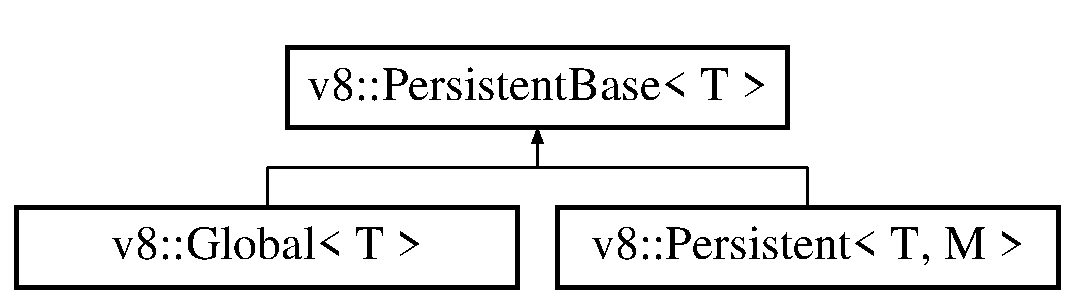
\includegraphics[height=2.000000cm]{classv8_1_1_persistent_base}
\end{center}
\end{figure}
\subsection*{Public Member Functions}
\begin{DoxyCompactItemize}
\item 
V8\+\_\+\+I\+N\+L\+I\+NE void \hyperlink{classv8_1_1_persistent_base_a174bb1e45b18fd4eeaee033622825bb8}{Reset} ()
\item 
{\footnotesize template$<$class S $>$ }\\V8\+\_\+\+I\+N\+L\+I\+NE void \hyperlink{classv8_1_1_persistent_base_a11164f0dfc9a16d79809236e7a9670aa}{Reset} (\hyperlink{classv8_1_1_isolate}{Isolate} $\ast$isolate, const \hyperlink{classv8_1_1_local}{Local}$<$ S $>$ \&other)
\item 
{\footnotesize template$<$class S $>$ }\\V8\+\_\+\+I\+N\+L\+I\+NE void \hyperlink{classv8_1_1_persistent_base_af6b8f929b0cbaa83341df48ca3b03ef5}{Reset} (\hyperlink{classv8_1_1_isolate}{Isolate} $\ast$isolate, const \hyperlink{classv8_1_1_persistent_base}{Persistent\+Base}$<$ S $>$ \&other)
\item 
V8\+\_\+\+I\+N\+L\+I\+NE bool {\bfseries Is\+Empty} () const \hypertarget{classv8_1_1_persistent_base_aa846b995b881b4863a21cf78ad7a8dea}{}\label{classv8_1_1_persistent_base_aa846b995b881b4863a21cf78ad7a8dea}

\item 
V8\+\_\+\+I\+N\+L\+I\+NE void {\bfseries Empty} ()\hypertarget{classv8_1_1_persistent_base_abb8a06471ea86de1731a3c94a879b00e}{}\label{classv8_1_1_persistent_base_abb8a06471ea86de1731a3c94a879b00e}

\item 
V8\+\_\+\+I\+N\+L\+I\+NE \hyperlink{classv8_1_1_local}{Local}$<$ T $>$ {\bfseries Get} (\hyperlink{classv8_1_1_isolate}{Isolate} $\ast$isolate) const \hypertarget{classv8_1_1_persistent_base_a46fddc38d4b77b73a5a1967542d3d557}{}\label{classv8_1_1_persistent_base_a46fddc38d4b77b73a5a1967542d3d557}

\item 
{\footnotesize template$<$class S $>$ }\\V8\+\_\+\+I\+N\+L\+I\+NE bool {\bfseries operator==} (const \hyperlink{classv8_1_1_persistent_base}{Persistent\+Base}$<$ S $>$ \&that) const \hypertarget{classv8_1_1_persistent_base_a6374a132dba19abcdece47cb2080aca7}{}\label{classv8_1_1_persistent_base_a6374a132dba19abcdece47cb2080aca7}

\item 
{\footnotesize template$<$class S $>$ }\\V8\+\_\+\+I\+N\+L\+I\+NE bool {\bfseries operator==} (const \hyperlink{classv8_1_1_local}{Local}$<$ S $>$ \&that) const \hypertarget{classv8_1_1_persistent_base_a5609a18c202901b6ab1b510fb3b0d1dc}{}\label{classv8_1_1_persistent_base_a5609a18c202901b6ab1b510fb3b0d1dc}

\item 
{\footnotesize template$<$class S $>$ }\\V8\+\_\+\+I\+N\+L\+I\+NE bool {\bfseries operator!=} (const \hyperlink{classv8_1_1_persistent_base}{Persistent\+Base}$<$ S $>$ \&that) const \hypertarget{classv8_1_1_persistent_base_a5bfacec9ab828f9aa7abdb980481589a}{}\label{classv8_1_1_persistent_base_a5bfacec9ab828f9aa7abdb980481589a}

\item 
{\footnotesize template$<$class S $>$ }\\V8\+\_\+\+I\+N\+L\+I\+NE bool {\bfseries operator!=} (const \hyperlink{classv8_1_1_local}{Local}$<$ S $>$ \&that) const \hypertarget{classv8_1_1_persistent_base_a467b78e40a53fb8324369d8a7a147800}{}\label{classv8_1_1_persistent_base_a467b78e40a53fb8324369d8a7a147800}

\item 
{\footnotesize template$<$typename P $>$ }\\V8\+\_\+\+I\+N\+L\+I\+NE \hyperlink{classv8_1_1_persistent_base_a64bcb00b5b075107304e0f1a867d15d4}{V8\+\_\+\+D\+E\+P\+R\+E\+C\+A\+T\+ED} (\char`\"{}use \hyperlink{classv8_1_1_weak_callback_info}{Weak\+Callback\+Info} version\char`\"{}, void Set\+Weak(P $\ast$parameter,                                                                   typename \hyperlink{classv8_1_1_weak_callback_data}{Weak\+Callback\+Data}$<$ T, P $>$\+::Callback callback))
\item 
{\footnotesize template$<$typename S , typename P $>$ }\\V8\+\_\+\+I\+N\+L\+I\+NE {\bfseries V8\+\_\+\+D\+E\+P\+R\+E\+C\+A\+T\+ED} (\char`\"{}use \hyperlink{classv8_1_1_weak_callback_info}{Weak\+Callback\+Info} version\char`\"{}, void Set\+Weak(P $\ast$parameter,                                                                   typename \hyperlink{classv8_1_1_weak_callback_data}{Weak\+Callback\+Data}$<$ S, P $>$\+::Callback callback))\hypertarget{classv8_1_1_persistent_base_a1e4aaa31c63db650c6db3bf6b976e8a1}{}\label{classv8_1_1_persistent_base_a1e4aaa31c63db650c6db3bf6b976e8a1}

\item 
{\footnotesize template$<$typename P $>$ }\\V8\+\_\+\+I\+N\+L\+I\+NE {\bfseries V8\+\_\+\+D\+E\+P\+R\+E\+C\+A\+T\+ED} (\char`\"{}use Set\+Weak\char`\"{}, void Set\+Phantom(P $\ast$parameter,                                                                               typename \hyperlink{classv8_1_1_weak_callback_info}{Weak\+Callback\+Info}$<$ P $>$\+::Callback callback,                                                                               int internal\+\_\+field\+\_\+index1=-\/1,                                                                               int internal\+\_\+field\+\_\+index2=-\/1))\hypertarget{classv8_1_1_persistent_base_ae717cd28f0b6f52a705e24a8b3b49b19}{}\label{classv8_1_1_persistent_base_ae717cd28f0b6f52a705e24a8b3b49b19}

\item 
{\footnotesize template$<$typename P $>$ }\\V8\+\_\+\+I\+N\+L\+I\+NE void {\bfseries Set\+Weak} (P $\ast$parameter, typename \hyperlink{classv8_1_1_weak_callback_info}{Weak\+Callback\+Info}$<$ P $>$\+::Callback callback, Weak\+Callback\+Type type)\hypertarget{classv8_1_1_persistent_base_aebb8a2c97e219102f613ff3749c956f6}{}\label{classv8_1_1_persistent_base_aebb8a2c97e219102f613ff3749c956f6}

\item 
{\footnotesize template$<$typename P $>$ }\\V8\+\_\+\+I\+N\+L\+I\+NE P $\ast$ {\bfseries Clear\+Weak} ()\hypertarget{classv8_1_1_persistent_base_a444d27c00650e3663348024df08cb121}{}\label{classv8_1_1_persistent_base_a444d27c00650e3663348024df08cb121}

\item 
V8\+\_\+\+I\+N\+L\+I\+NE void {\bfseries Clear\+Weak} ()\hypertarget{classv8_1_1_persistent_base_afe515daead108cceb1699b54051df13b}{}\label{classv8_1_1_persistent_base_afe515daead108cceb1699b54051df13b}

\item 
V8\+\_\+\+I\+N\+L\+I\+NE void \hyperlink{classv8_1_1_persistent_base_a14c051e0080bbe7fbe02be35865b9923}{Register\+External\+Reference} (\hyperlink{classv8_1_1_isolate}{Isolate} $\ast$isolate) const 
\item 
V8\+\_\+\+I\+N\+L\+I\+NE void \hyperlink{classv8_1_1_persistent_base_aed12b0a54bc5ade1fb44e3bdb3a1fe74}{Mark\+Independent} ()
\item 
V8\+\_\+\+I\+N\+L\+I\+NE \hyperlink{classv8_1_1_persistent_base_af18132d6f1472d42d101b1bb410505cb}{V8\+\_\+\+D\+E\+P\+R\+E\+C\+A\+T\+ED} (\char`\"{}deprecated optimization, do not use partially dependent groups\char`\"{}, void Mark\+Partially\+Dependent())
\item 
V8\+\_\+\+I\+N\+L\+I\+NE void \hyperlink{classv8_1_1_persistent_base_a7244edd33a45b7d95e566fce85e3f87d}{Mark\+Active} ()
\item 
V8\+\_\+\+I\+N\+L\+I\+NE bool {\bfseries Is\+Independent} () const \hypertarget{classv8_1_1_persistent_base_a2ed93b6be1b27c299906935ef35d2114}{}\label{classv8_1_1_persistent_base_a2ed93b6be1b27c299906935ef35d2114}

\item 
V8\+\_\+\+I\+N\+L\+I\+NE bool \hyperlink{classv8_1_1_persistent_base_a4a64c26d91ed6a276aa8a7ca4bb7683a}{Is\+Near\+Death} () const 
\item 
V8\+\_\+\+I\+N\+L\+I\+NE bool \hyperlink{classv8_1_1_persistent_base_a714b7794149df483837a2c6b09d52396}{Is\+Weak} () const 
\item 
V8\+\_\+\+I\+N\+L\+I\+NE void \hyperlink{classv8_1_1_persistent_base_ac4c979164b3ed4dc92319e6f5a108d3d}{Set\+Wrapper\+Class\+Id} (uint16\+\_\+t class\+\_\+id)
\item 
V8\+\_\+\+I\+N\+L\+I\+NE uint16\+\_\+t \hyperlink{classv8_1_1_persistent_base_a01a46bf4e69ed9a837639702ee234643}{Wrapper\+Class\+Id} () const 
\item 
{\footnotesize template$<$class S $>$ }\\void {\bfseries Reset} (\hyperlink{classv8_1_1_isolate}{Isolate} $\ast$isolate, const \hyperlink{classv8_1_1_local}{Local}$<$ S $>$ \&other)\hypertarget{classv8_1_1_persistent_base_ab4b4d3fba3498486f1f10dc7d5be90fc}{}\label{classv8_1_1_persistent_base_ab4b4d3fba3498486f1f10dc7d5be90fc}

\item 
{\footnotesize template$<$class S $>$ }\\void {\bfseries Reset} (\hyperlink{classv8_1_1_isolate}{Isolate} $\ast$isolate, const \hyperlink{classv8_1_1_persistent_base}{Persistent\+Base}$<$ S $>$ \&other)\hypertarget{classv8_1_1_persistent_base_a67cbcedf77d176d3870fa4993e300b61}{}\label{classv8_1_1_persistent_base_a67cbcedf77d176d3870fa4993e300b61}

\item 
{\footnotesize template$<$typename P $>$ }\\void {\bfseries Set\+Weak} (P $\ast$parameter, typename \hyperlink{classv8_1_1_weak_callback_data}{Weak\+Callback\+Data}$<$ T, P $>$\+::Callback callback)\hypertarget{classv8_1_1_persistent_base_aaf342ece1a4ba926ba62e8d6af7be777}{}\label{classv8_1_1_persistent_base_aaf342ece1a4ba926ba62e8d6af7be777}

\end{DoxyCompactItemize}
\subsection*{Private Member Functions}
\begin{DoxyCompactItemize}
\item 
V8\+\_\+\+I\+N\+L\+I\+NE {\bfseries Persistent\+Base} (T $\ast$val)\hypertarget{classv8_1_1_persistent_base_a69c26b1d8849c8905a162db8f058cf0e}{}\label{classv8_1_1_persistent_base_a69c26b1d8849c8905a162db8f058cf0e}

\item 
{\bfseries Persistent\+Base} (const \hyperlink{classv8_1_1_persistent_base}{Persistent\+Base} \&other)=delete\hypertarget{classv8_1_1_persistent_base_aa403ece93fda904f5d6ab39e9383a504}{}\label{classv8_1_1_persistent_base_aa403ece93fda904f5d6ab39e9383a504}

\item 
void {\bfseries operator=} (const \hyperlink{classv8_1_1_persistent_base}{Persistent\+Base} \&)=delete\hypertarget{classv8_1_1_persistent_base_ada3d83b8cadaf4b83027baa41cd99d8c}{}\label{classv8_1_1_persistent_base_ada3d83b8cadaf4b83027baa41cd99d8c}

\end{DoxyCompactItemize}
\subsection*{Static Private Member Functions}
\begin{DoxyCompactItemize}
\item 
static V8\+\_\+\+I\+N\+L\+I\+NE T $\ast$ {\bfseries New} (\hyperlink{classv8_1_1_isolate}{Isolate} $\ast$isolate, T $\ast$that)\hypertarget{classv8_1_1_persistent_base_ae5d4014fe651f1d7753c96147b04dd00}{}\label{classv8_1_1_persistent_base_ae5d4014fe651f1d7753c96147b04dd00}

\end{DoxyCompactItemize}
\subsection*{Private Attributes}
\begin{DoxyCompactItemize}
\item 
T $\ast$ {\bfseries val\+\_\+}\hypertarget{classv8_1_1_persistent_base_a380d24a680b9112e999dccf51d7e2d68}{}\label{classv8_1_1_persistent_base_a380d24a680b9112e999dccf51d7e2d68}

\end{DoxyCompactItemize}
\subsection*{Friends}
\begin{DoxyCompactItemize}
\item 
class {\bfseries Isolate}\hypertarget{classv8_1_1_persistent_base_aba4f0964bdacf2bbf62cf876e5d28d0a}{}\label{classv8_1_1_persistent_base_aba4f0964bdacf2bbf62cf876e5d28d0a}

\item 
class {\bfseries Utils}\hypertarget{classv8_1_1_persistent_base_abc0f7da619e9e72510dc07ed7b5ff6d8}{}\label{classv8_1_1_persistent_base_abc0f7da619e9e72510dc07ed7b5ff6d8}

\item 
{\footnotesize template$<$class F $>$ }\\class {\bfseries Local}\hypertarget{classv8_1_1_persistent_base_afb872edb4aac7ba55f0da004113aa2b0}{}\label{classv8_1_1_persistent_base_afb872edb4aac7ba55f0da004113aa2b0}

\item 
{\footnotesize template$<$class F1 , class F2 $>$ }\\class {\bfseries Persistent}\hypertarget{classv8_1_1_persistent_base_ad845ec8872174be0a9ca9a3dd1898d30}{}\label{classv8_1_1_persistent_base_ad845ec8872174be0a9ca9a3dd1898d30}

\item 
{\footnotesize template$<$class F $>$ }\\class {\bfseries Global}\hypertarget{classv8_1_1_persistent_base_adc49d0fc7441cf7e3b5f039334e44243}{}\label{classv8_1_1_persistent_base_adc49d0fc7441cf7e3b5f039334e44243}

\item 
{\footnotesize template$<$class F $>$ }\\class {\bfseries Persistent\+Base}\hypertarget{classv8_1_1_persistent_base_abb172e0bb22fc5fed7a3a66f29d046ce}{}\label{classv8_1_1_persistent_base_abb172e0bb22fc5fed7a3a66f29d046ce}

\item 
{\footnotesize template$<$class F $>$ }\\class {\bfseries Return\+Value}\hypertarget{classv8_1_1_persistent_base_a53f604d3d6f2dc0647df33c9979f116a}{}\label{classv8_1_1_persistent_base_a53f604d3d6f2dc0647df33c9979f116a}

\item 
{\footnotesize template$<$class F1 , class F2 , class F3 $>$ }\\class {\bfseries Persistent\+Value\+Map\+Base}\hypertarget{classv8_1_1_persistent_base_a08e2b8f164392d71811ce6cc134f33e3}{}\label{classv8_1_1_persistent_base_a08e2b8f164392d71811ce6cc134f33e3}

\item 
{\footnotesize template$<$class F1 , class F2 $>$ }\\class {\bfseries Persistent\+Value\+Vector}\hypertarget{classv8_1_1_persistent_base_a978bb1377559897d74d5fe883a54a315}{}\label{classv8_1_1_persistent_base_a978bb1377559897d74d5fe883a54a315}

\item 
class {\bfseries Object}\hypertarget{classv8_1_1_persistent_base_a0720b5f434e636e22a3ed34f847eec57}{}\label{classv8_1_1_persistent_base_a0720b5f434e636e22a3ed34f847eec57}

\end{DoxyCompactItemize}


\subsection{Detailed Description}
\subsubsection*{template$<$class T$>$\\*
class v8\+::\+Persistent\+Base$<$ T $>$}

An object reference that is independent of any handle scope. Where a \hyperlink{classv8_1_1_local}{Local} handle only lives as long as the \hyperlink{classv8_1_1_handle_scope}{Handle\+Scope} in which it was allocated, a \hyperlink{classv8_1_1_persistent_base}{Persistent\+Base} handle remains valid until it is explicitly disposed.

A persistent handle contains a reference to a storage cell within the \hyperlink{namespacev8}{v8} engine which holds an object value and which is updated by the garbage collector whenever the object is moved. A new storage cell can be created using the constructor or \hyperlink{classv8_1_1_persistent_base_a174bb1e45b18fd4eeaee033622825bb8}{Persistent\+Base\+::\+Reset} and existing handles can be disposed using \hyperlink{classv8_1_1_persistent_base_a174bb1e45b18fd4eeaee033622825bb8}{Persistent\+Base\+::\+Reset}. 

\subsection{Member Function Documentation}
\index{v8\+::\+Persistent\+Base@{v8\+::\+Persistent\+Base}!Is\+Near\+Death@{Is\+Near\+Death}}
\index{Is\+Near\+Death@{Is\+Near\+Death}!v8\+::\+Persistent\+Base@{v8\+::\+Persistent\+Base}}
\subsubsection[{\texorpdfstring{Is\+Near\+Death() const }{IsNearDeath() const }}]{\setlength{\rightskip}{0pt plus 5cm}template$<$class T $>$ bool {\bf v8\+::\+Persistent\+Base}$<$ T $>$\+::Is\+Near\+Death (
\begin{DoxyParamCaption}
{}
\end{DoxyParamCaption}
) const}\hypertarget{classv8_1_1_persistent_base_a4a64c26d91ed6a276aa8a7ca4bb7683a}{}\label{classv8_1_1_persistent_base_a4a64c26d91ed6a276aa8a7ca4bb7683a}
Checks if the handle holds the only reference to an object. \index{v8\+::\+Persistent\+Base@{v8\+::\+Persistent\+Base}!Is\+Weak@{Is\+Weak}}
\index{Is\+Weak@{Is\+Weak}!v8\+::\+Persistent\+Base@{v8\+::\+Persistent\+Base}}
\subsubsection[{\texorpdfstring{Is\+Weak() const }{IsWeak() const }}]{\setlength{\rightskip}{0pt plus 5cm}template$<$class T $>$ bool {\bf v8\+::\+Persistent\+Base}$<$ T $>$\+::Is\+Weak (
\begin{DoxyParamCaption}
{}
\end{DoxyParamCaption}
) const}\hypertarget{classv8_1_1_persistent_base_a714b7794149df483837a2c6b09d52396}{}\label{classv8_1_1_persistent_base_a714b7794149df483837a2c6b09d52396}
Returns true if the handle\textquotesingle{}s reference is weak. \index{v8\+::\+Persistent\+Base@{v8\+::\+Persistent\+Base}!Mark\+Active@{Mark\+Active}}
\index{Mark\+Active@{Mark\+Active}!v8\+::\+Persistent\+Base@{v8\+::\+Persistent\+Base}}
\subsubsection[{\texorpdfstring{Mark\+Active()}{MarkActive()}}]{\setlength{\rightskip}{0pt plus 5cm}template$<$class T $>$ void {\bf v8\+::\+Persistent\+Base}$<$ T $>$\+::Mark\+Active (
\begin{DoxyParamCaption}
{}
\end{DoxyParamCaption}
)}\hypertarget{classv8_1_1_persistent_base_a7244edd33a45b7d95e566fce85e3f87d}{}\label{classv8_1_1_persistent_base_a7244edd33a45b7d95e566fce85e3f87d}
Marks the reference to this object as active. The scavenge garbage collection should not reclaim the objects marked as active. This bit is cleared after the each garbage collection pass. \index{v8\+::\+Persistent\+Base@{v8\+::\+Persistent\+Base}!Mark\+Independent@{Mark\+Independent}}
\index{Mark\+Independent@{Mark\+Independent}!v8\+::\+Persistent\+Base@{v8\+::\+Persistent\+Base}}
\subsubsection[{\texorpdfstring{Mark\+Independent()}{MarkIndependent()}}]{\setlength{\rightskip}{0pt plus 5cm}template$<$class T $>$ void {\bf v8\+::\+Persistent\+Base}$<$ T $>$\+::Mark\+Independent (
\begin{DoxyParamCaption}
{}
\end{DoxyParamCaption}
)}\hypertarget{classv8_1_1_persistent_base_aed12b0a54bc5ade1fb44e3bdb3a1fe74}{}\label{classv8_1_1_persistent_base_aed12b0a54bc5ade1fb44e3bdb3a1fe74}
Marks the reference to this object independent. Garbage collector is free to ignore any object groups containing this object. Weak callback for an independent handle should not assume that it will be preceded by a global GC prologue callback or followed by a global GC epilogue callback. \index{v8\+::\+Persistent\+Base@{v8\+::\+Persistent\+Base}!Register\+External\+Reference@{Register\+External\+Reference}}
\index{Register\+External\+Reference@{Register\+External\+Reference}!v8\+::\+Persistent\+Base@{v8\+::\+Persistent\+Base}}
\subsubsection[{\texorpdfstring{Register\+External\+Reference(\+Isolate $\ast$isolate) const }{RegisterExternalReference(Isolate *isolate) const }}]{\setlength{\rightskip}{0pt plus 5cm}template$<$class T $>$ void {\bf v8\+::\+Persistent\+Base}$<$ T $>$\+::Register\+External\+Reference (
\begin{DoxyParamCaption}
\item[{{\bf Isolate} $\ast$}]{isolate}
\end{DoxyParamCaption}
) const}\hypertarget{classv8_1_1_persistent_base_a14c051e0080bbe7fbe02be35865b9923}{}\label{classv8_1_1_persistent_base_a14c051e0080bbe7fbe02be35865b9923}
Allows the embedder to tell the \hyperlink{namespacev8}{v8} garbage collector that a certain object is alive. Only allowed when the embedder is asked to trace its heap by \hyperlink{classv8_1_1_embedder_heap_tracer}{Embedder\+Heap\+Tracer}. \index{v8\+::\+Persistent\+Base@{v8\+::\+Persistent\+Base}!Reset@{Reset}}
\index{Reset@{Reset}!v8\+::\+Persistent\+Base@{v8\+::\+Persistent\+Base}}
\subsubsection[{\texorpdfstring{Reset()}{Reset()}}]{\setlength{\rightskip}{0pt plus 5cm}template$<$class T $>$ void {\bf v8\+::\+Persistent\+Base}$<$ T $>$\+::Reset (
\begin{DoxyParamCaption}
{}
\end{DoxyParamCaption}
)}\hypertarget{classv8_1_1_persistent_base_a174bb1e45b18fd4eeaee033622825bb8}{}\label{classv8_1_1_persistent_base_a174bb1e45b18fd4eeaee033622825bb8}
If non-\/empty, destroy the underlying storage cell Is\+Empty() will return true after this call. \index{v8\+::\+Persistent\+Base@{v8\+::\+Persistent\+Base}!Reset@{Reset}}
\index{Reset@{Reset}!v8\+::\+Persistent\+Base@{v8\+::\+Persistent\+Base}}
\subsubsection[{\texorpdfstring{Reset(\+Isolate $\ast$isolate, const Local$<$ S $>$ \&other)}{Reset(Isolate *isolate, const Local< S > &other)}}]{\setlength{\rightskip}{0pt plus 5cm}template$<$class T$>$ template$<$class S $>$ V8\+\_\+\+I\+N\+L\+I\+NE void {\bf v8\+::\+Persistent\+Base}$<$ T $>$\+::Reset (
\begin{DoxyParamCaption}
\item[{{\bf Isolate} $\ast$}]{isolate, }
\item[{const {\bf Local}$<$ S $>$ \&}]{other}
\end{DoxyParamCaption}
)}\hypertarget{classv8_1_1_persistent_base_a11164f0dfc9a16d79809236e7a9670aa}{}\label{classv8_1_1_persistent_base_a11164f0dfc9a16d79809236e7a9670aa}
If non-\/empty, destroy the underlying storage cell and create a new one with the contents of other if other is non empty \index{v8\+::\+Persistent\+Base@{v8\+::\+Persistent\+Base}!Reset@{Reset}}
\index{Reset@{Reset}!v8\+::\+Persistent\+Base@{v8\+::\+Persistent\+Base}}
\subsubsection[{\texorpdfstring{Reset(\+Isolate $\ast$isolate, const Persistent\+Base$<$ S $>$ \&other)}{Reset(Isolate *isolate, const PersistentBase< S > &other)}}]{\setlength{\rightskip}{0pt plus 5cm}template$<$class T$>$ template$<$class S $>$ V8\+\_\+\+I\+N\+L\+I\+NE void {\bf v8\+::\+Persistent\+Base}$<$ T $>$\+::Reset (
\begin{DoxyParamCaption}
\item[{{\bf Isolate} $\ast$}]{isolate, }
\item[{const {\bf Persistent\+Base}$<$ S $>$ \&}]{other}
\end{DoxyParamCaption}
)}\hypertarget{classv8_1_1_persistent_base_af6b8f929b0cbaa83341df48ca3b03ef5}{}\label{classv8_1_1_persistent_base_af6b8f929b0cbaa83341df48ca3b03ef5}
If non-\/empty, destroy the underlying storage cell and create a new one with the contents of other if other is non empty \index{v8\+::\+Persistent\+Base@{v8\+::\+Persistent\+Base}!Set\+Wrapper\+Class\+Id@{Set\+Wrapper\+Class\+Id}}
\index{Set\+Wrapper\+Class\+Id@{Set\+Wrapper\+Class\+Id}!v8\+::\+Persistent\+Base@{v8\+::\+Persistent\+Base}}
\subsubsection[{\texorpdfstring{Set\+Wrapper\+Class\+Id(uint16\+\_\+t class\+\_\+id)}{SetWrapperClassId(uint16_t class_id)}}]{\setlength{\rightskip}{0pt plus 5cm}template$<$class T $>$ void {\bf v8\+::\+Persistent\+Base}$<$ T $>$\+::Set\+Wrapper\+Class\+Id (
\begin{DoxyParamCaption}
\item[{uint16\+\_\+t}]{class\+\_\+id}
\end{DoxyParamCaption}
)}\hypertarget{classv8_1_1_persistent_base_ac4c979164b3ed4dc92319e6f5a108d3d}{}\label{classv8_1_1_persistent_base_ac4c979164b3ed4dc92319e6f5a108d3d}
Assigns a wrapper class ID to the handle. See \hyperlink{classv8_1_1_retained_object_info}{Retained\+Object\+Info} interface description in \hyperlink{v8-profiler_8h_source}{v8-\/profiler.\+h} for details. \index{v8\+::\+Persistent\+Base@{v8\+::\+Persistent\+Base}!V8\+\_\+\+D\+E\+P\+R\+E\+C\+A\+T\+ED@{V8\+\_\+\+D\+E\+P\+R\+E\+C\+A\+T\+ED}}
\index{V8\+\_\+\+D\+E\+P\+R\+E\+C\+A\+T\+ED@{V8\+\_\+\+D\+E\+P\+R\+E\+C\+A\+T\+ED}!v8\+::\+Persistent\+Base@{v8\+::\+Persistent\+Base}}
\subsubsection[{\texorpdfstring{V8\+\_\+\+D\+E\+P\+R\+E\+C\+A\+T\+E\+D(""use Weak\+Callback\+Info version"", void Set\+Weak(\+P $\ast$parameter,                                                                   typename Weak\+Callback\+Data$<$ T, P $>$\+::\+Callback callback))}{V8_DEPRECATED("use WeakCallbackInfo version", void SetWeak(P *parameter,                                                                   typename WeakCallbackData< T, P >::Callback callback))}}]{\setlength{\rightskip}{0pt plus 5cm}template$<$class T$>$ template$<$typename P $>$ V8\+\_\+\+I\+N\+L\+I\+NE {\bf v8\+::\+Persistent\+Base}$<$ T $>$\+::V8\+\_\+\+D\+E\+P\+R\+E\+C\+A\+T\+ED (
\begin{DoxyParamCaption}
\item[{\char`\"{}use {\bf Weak\+Callback\+Info} version\char`\"{}}]{, }
\item[{void }]{Set\+WeakP $\ast$parameter,                                                                                                                                   typename Weak\+Callback\+Data$<$ T, P $>$\+::\+Callback callback}
\end{DoxyParamCaption}
)}\hypertarget{classv8_1_1_persistent_base_a64bcb00b5b075107304e0f1a867d15d4}{}\label{classv8_1_1_persistent_base_a64bcb00b5b075107304e0f1a867d15d4}
Install a finalization callback on this object. N\+O\+TE\+: There is no guarantee as to {\itshape when} or even {\itshape if} the callback is invoked. The invocation is performed solely on a best effort basis. As always, G\+C-\/based finalization should {\itshape not} be relied upon for any critical form of resource management! \index{v8\+::\+Persistent\+Base@{v8\+::\+Persistent\+Base}!V8\+\_\+\+D\+E\+P\+R\+E\+C\+A\+T\+ED@{V8\+\_\+\+D\+E\+P\+R\+E\+C\+A\+T\+ED}}
\index{V8\+\_\+\+D\+E\+P\+R\+E\+C\+A\+T\+ED@{V8\+\_\+\+D\+E\+P\+R\+E\+C\+A\+T\+ED}!v8\+::\+Persistent\+Base@{v8\+::\+Persistent\+Base}}
\subsubsection[{\texorpdfstring{V8\+\_\+\+D\+E\+P\+R\+E\+C\+A\+T\+E\+D(""deprecated optimization, do not use partially dependent groups"", void Mark\+Partially\+Dependent())}{V8_DEPRECATED("deprecated optimization, do not use partially dependent groups", void MarkPartiallyDependent())}}]{\setlength{\rightskip}{0pt plus 5cm}template$<$class T$>$ V8\+\_\+\+I\+N\+L\+I\+NE {\bf v8\+::\+Persistent\+Base}$<$ T $>$\+::V8\+\_\+\+D\+E\+P\+R\+E\+C\+A\+T\+ED (
\begin{DoxyParamCaption}
\item[{\char`\"{}deprecated}]{optimization, }
\item[{do not use partially dependent groups\char`\"{}}]{, }
\item[{void }]{Mark\+Partially\+Dependent()}
\end{DoxyParamCaption}
)}\hypertarget{classv8_1_1_persistent_base_af18132d6f1472d42d101b1bb410505cb}{}\label{classv8_1_1_persistent_base_af18132d6f1472d42d101b1bb410505cb}
Marks the reference to this object partially dependent. Partially dependent handles only depend on other partially dependent handles and these dependencies are provided through object groups. It provides a way to build smaller object groups for young objects that represent only a subset of all external dependencies. This mark is automatically cleared after each garbage collection. \index{v8\+::\+Persistent\+Base@{v8\+::\+Persistent\+Base}!Wrapper\+Class\+Id@{Wrapper\+Class\+Id}}
\index{Wrapper\+Class\+Id@{Wrapper\+Class\+Id}!v8\+::\+Persistent\+Base@{v8\+::\+Persistent\+Base}}
\subsubsection[{\texorpdfstring{Wrapper\+Class\+Id() const }{WrapperClassId() const }}]{\setlength{\rightskip}{0pt plus 5cm}template$<$class T $>$ uint16\+\_\+t {\bf v8\+::\+Persistent\+Base}$<$ T $>$\+::Wrapper\+Class\+Id (
\begin{DoxyParamCaption}
{}
\end{DoxyParamCaption}
) const}\hypertarget{classv8_1_1_persistent_base_a01a46bf4e69ed9a837639702ee234643}{}\label{classv8_1_1_persistent_base_a01a46bf4e69ed9a837639702ee234643}
Returns the class ID previously assigned to this handle or 0 if no class ID was previously assigned. 

The documentation for this class was generated from the following file\+:\begin{DoxyCompactItemize}
\item 
include/v8.\+h\end{DoxyCompactItemize}

\hypertarget{classv8_1_1_persistent_handle_visitor}{}\section{v8\+:\+:Persistent\+Handle\+Visitor Class Reference}
\label{classv8_1_1_persistent_handle_visitor}\index{v8\+::\+Persistent\+Handle\+Visitor@{v8\+::\+Persistent\+Handle\+Visitor}}


{\ttfamily \#include $<$v8.\+h$>$}

\subsection*{Public Member Functions}
\begin{DoxyCompactItemize}
\item 
virtual void {\bfseries Visit\+Persistent\+Handle} (\hyperlink{classv8_1_1_persistent}{Persistent}$<$ \hyperlink{classv8_1_1_value}{Value} $>$ $\ast$value, uint16\+\_\+t class\+\_\+id)\hypertarget{classv8_1_1_persistent_handle_visitor_a092c6cc7700b38d9c60bd693a071045a}{}\label{classv8_1_1_persistent_handle_visitor_a092c6cc7700b38d9c60bd693a071045a}

\end{DoxyCompactItemize}


\subsection{Detailed Description}
Interface for iterating through all the persistent handles in the heap. 

The documentation for this class was generated from the following file\+:\begin{DoxyCompactItemize}
\item 
/\+Users/joshgav/node/v8/include/v8.\+h\end{DoxyCompactItemize}

\hypertarget{classv8_1_1_persistent_value_map}{}\section{v8\+:\+:Persistent\+Value\+Map$<$ K, V, Traits $>$ Class Template Reference}
\label{classv8_1_1_persistent_value_map}\index{v8\+::\+Persistent\+Value\+Map$<$ K, V, Traits $>$@{v8\+::\+Persistent\+Value\+Map$<$ K, V, Traits $>$}}
Inheritance diagram for v8\+:\+:Persistent\+Value\+Map$<$ K, V, Traits $>$\+:\begin{figure}[H]
\begin{center}
\leavevmode
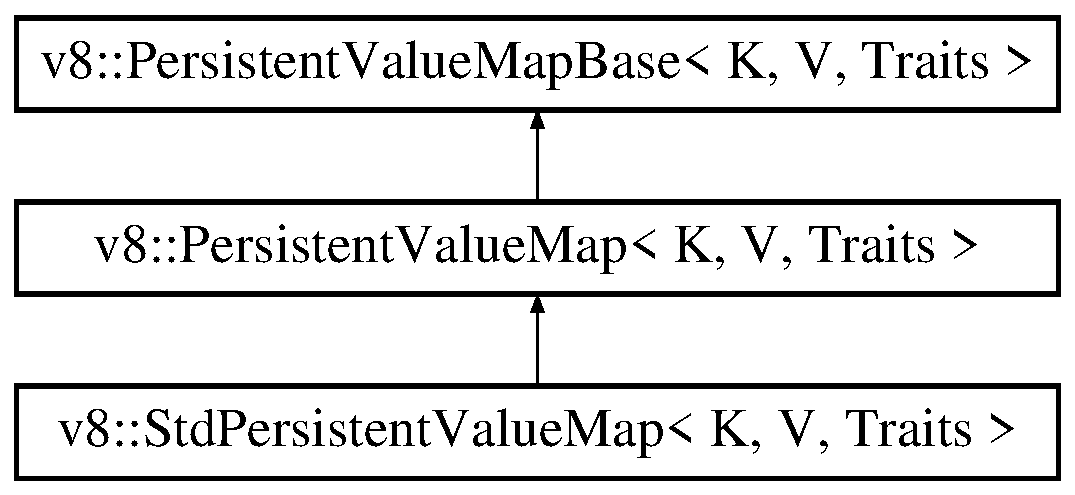
\includegraphics[height=3.000000cm]{classv8_1_1_persistent_value_map}
\end{center}
\end{figure}
\subsection*{Public Types}
\begin{DoxyCompactItemize}
\item 
typedef \hyperlink{classv8_1_1_persistent_value_map_base}{Persistent\+Value\+Map\+Base}$<$ K, V, Traits $>$\+::\hyperlink{classv8_1_1_persistent_value_map_base_1_1_persistent_value_reference}{Persistent\+Value\+Reference} {\bfseries Persistent\+Value\+Reference}\hypertarget{classv8_1_1_persistent_value_map_a81ed968e13bcef1cd97a09fd024f30f2}{}\label{classv8_1_1_persistent_value_map_a81ed968e13bcef1cd97a09fd024f30f2}

\end{DoxyCompactItemize}
\subsection*{Public Member Functions}
\begin{DoxyCompactItemize}
\item 
{\bfseries Persistent\+Value\+Map} (\hyperlink{classv8_1_1_isolate}{Isolate} $\ast$isolate)\hypertarget{classv8_1_1_persistent_value_map_af8000a75ef84fa719724dc4dadc1e5ee}{}\label{classv8_1_1_persistent_value_map_af8000a75ef84fa719724dc4dadc1e5ee}

\item 
\hyperlink{classv8_1_1_global}{Global}$<$ V $>$ \hyperlink{classv8_1_1_persistent_value_map_a4527a2e1b25a9f1772317f948382d9f9}{Set} (const K \&key, \hyperlink{classv8_1_1_local}{Local}$<$ V $>$ value)
\item 
\hyperlink{classv8_1_1_global}{Global}$<$ V $>$ \hyperlink{classv8_1_1_persistent_value_map_a00f89f1b7665698349f98b04d0059180}{Set} (const K \&key, \hyperlink{classv8_1_1_global}{Global}$<$ V $>$ value)
\item 
\hyperlink{classv8_1_1_global}{Global}$<$ V $>$ \hyperlink{classv8_1_1_persistent_value_map_a97ab74c7670e65dd5f95ec2940c4ab11}{Set\+Unique} (const K \&key, \hyperlink{classv8_1_1_global}{Global}$<$ V $>$ $\ast$persistent)
\item 
\hyperlink{classv8_1_1_global}{Global}$<$ V $>$ \hyperlink{classv8_1_1_persistent_value_map_a8128f8cff6ed0f3177e966b28cc081ba}{Set} (const K \&key, \hyperlink{classv8_1_1_global}{Global}$<$ V $>$ value, \hyperlink{classv8_1_1_persistent_value_map_base_1_1_persistent_value_reference}{Persistent\+Value\+Reference} $\ast$reference)
\end{DoxyCompactItemize}
\subsection*{Static Private Member Functions}
\begin{DoxyCompactItemize}
\item 
static void {\bfseries Weak\+Callback} (const \hyperlink{classv8_1_1_weak_callback_data}{Weak\+Callback\+Data}$<$ V, typename Traits\+::\+Weak\+Callback\+Data\+Type $>$ \&data)\hypertarget{classv8_1_1_persistent_value_map_a3666c5e5d35faec5b824f41c37fd8be1}{}\label{classv8_1_1_persistent_value_map_a3666c5e5d35faec5b824f41c37fd8be1}

\end{DoxyCompactItemize}
\subsection*{Additional Inherited Members}


\subsection{Member Function Documentation}
\index{v8\+::\+Persistent\+Value\+Map@{v8\+::\+Persistent\+Value\+Map}!Set@{Set}}
\index{Set@{Set}!v8\+::\+Persistent\+Value\+Map@{v8\+::\+Persistent\+Value\+Map}}
\subsubsection[{\texorpdfstring{Set(const K \&key, Local$<$ V $>$ value)}{Set(const K &key, Local< V > value)}}]{\setlength{\rightskip}{0pt plus 5cm}template$<$typename K, typename V, typename Traits$>$ {\bf Global}$<$V$>$ {\bf v8\+::\+Persistent\+Value\+Map}$<$ K, V, Traits $>$\+::{\bf Set} (
\begin{DoxyParamCaption}
\item[{const K \&}]{key, }
\item[{{\bf Local}$<$ V $>$}]{value}
\end{DoxyParamCaption}
)\hspace{0.3cm}{\ttfamily [inline]}}\hypertarget{classv8_1_1_persistent_value_map_a4527a2e1b25a9f1772317f948382d9f9}{}\label{classv8_1_1_persistent_value_map_a4527a2e1b25a9f1772317f948382d9f9}
Put value into map. Depending on Traits\+::k\+Is\+Weak, the value will be held by the map strongly or weakly. Returns old value as \hyperlink{classv8_1_1_global}{Global}. \index{v8\+::\+Persistent\+Value\+Map@{v8\+::\+Persistent\+Value\+Map}!Set@{Set}}
\index{Set@{Set}!v8\+::\+Persistent\+Value\+Map@{v8\+::\+Persistent\+Value\+Map}}
\subsubsection[{\texorpdfstring{Set(const K \&key, Global$<$ V $>$ value)}{Set(const K &key, Global< V > value)}}]{\setlength{\rightskip}{0pt plus 5cm}template$<$typename K, typename V, typename Traits$>$ {\bf Global}$<$V$>$ {\bf v8\+::\+Persistent\+Value\+Map}$<$ K, V, Traits $>$\+::{\bf Set} (
\begin{DoxyParamCaption}
\item[{const K \&}]{key, }
\item[{{\bf Global}$<$ V $>$}]{value}
\end{DoxyParamCaption}
)\hspace{0.3cm}{\ttfamily [inline]}}\hypertarget{classv8_1_1_persistent_value_map_a00f89f1b7665698349f98b04d0059180}{}\label{classv8_1_1_persistent_value_map_a00f89f1b7665698349f98b04d0059180}
Put value into map, like \hyperlink{classv8_1_1_persistent_value_map_a4527a2e1b25a9f1772317f948382d9f9}{Set(const K\&, Local$<$\+V$>$)}. \index{v8\+::\+Persistent\+Value\+Map@{v8\+::\+Persistent\+Value\+Map}!Set@{Set}}
\index{Set@{Set}!v8\+::\+Persistent\+Value\+Map@{v8\+::\+Persistent\+Value\+Map}}
\subsubsection[{\texorpdfstring{Set(const K \&key, Global$<$ V $>$ value, Persistent\+Value\+Reference $\ast$reference)}{Set(const K &key, Global< V > value, PersistentValueReference *reference)}}]{\setlength{\rightskip}{0pt plus 5cm}template$<$typename K, typename V, typename Traits$>$ {\bf Global}$<$V$>$ {\bf v8\+::\+Persistent\+Value\+Map}$<$ K, V, Traits $>$\+::{\bf Set} (
\begin{DoxyParamCaption}
\item[{const K \&}]{key, }
\item[{{\bf Global}$<$ V $>$}]{value, }
\item[{{\bf Persistent\+Value\+Reference} $\ast$}]{reference}
\end{DoxyParamCaption}
)\hspace{0.3cm}{\ttfamily [inline]}}\hypertarget{classv8_1_1_persistent_value_map_a8128f8cff6ed0f3177e966b28cc081ba}{}\label{classv8_1_1_persistent_value_map_a8128f8cff6ed0f3177e966b28cc081ba}
Put a value into the map and update the reference. Restrictions of Get\+Reference apply here as well. \index{v8\+::\+Persistent\+Value\+Map@{v8\+::\+Persistent\+Value\+Map}!Set\+Unique@{Set\+Unique}}
\index{Set\+Unique@{Set\+Unique}!v8\+::\+Persistent\+Value\+Map@{v8\+::\+Persistent\+Value\+Map}}
\subsubsection[{\texorpdfstring{Set\+Unique(const K \&key, Global$<$ V $>$ $\ast$persistent)}{SetUnique(const K &key, Global< V > *persistent)}}]{\setlength{\rightskip}{0pt plus 5cm}template$<$typename K, typename V, typename Traits$>$ {\bf Global}$<$V$>$ {\bf v8\+::\+Persistent\+Value\+Map}$<$ K, V, Traits $>$\+::Set\+Unique (
\begin{DoxyParamCaption}
\item[{const K \&}]{key, }
\item[{{\bf Global}$<$ V $>$ $\ast$}]{persistent}
\end{DoxyParamCaption}
)\hspace{0.3cm}{\ttfamily [inline]}}\hypertarget{classv8_1_1_persistent_value_map_a97ab74c7670e65dd5f95ec2940c4ab11}{}\label{classv8_1_1_persistent_value_map_a97ab74c7670e65dd5f95ec2940c4ab11}
Put the value into the map, and set the \textquotesingle{}weak\textquotesingle{} callback when demanded by the Traits class. 

The documentation for this class was generated from the following file\+:\begin{DoxyCompactItemize}
\item 
include/v8-\/util.\+h\end{DoxyCompactItemize}

\hypertarget{classv8_1_1_persistent_value_map_base}{}\section{v8\+:\+:Persistent\+Value\+Map\+Base$<$ K, V, Traits $>$ Class Template Reference}
\label{classv8_1_1_persistent_value_map_base}\index{v8\+::\+Persistent\+Value\+Map\+Base$<$ K, V, Traits $>$@{v8\+::\+Persistent\+Value\+Map\+Base$<$ K, V, Traits $>$}}


{\ttfamily \#include $<$v8-\/util.\+h$>$}

Inheritance diagram for v8\+:\+:Persistent\+Value\+Map\+Base$<$ K, V, Traits $>$\+:\begin{figure}[H]
\begin{center}
\leavevmode
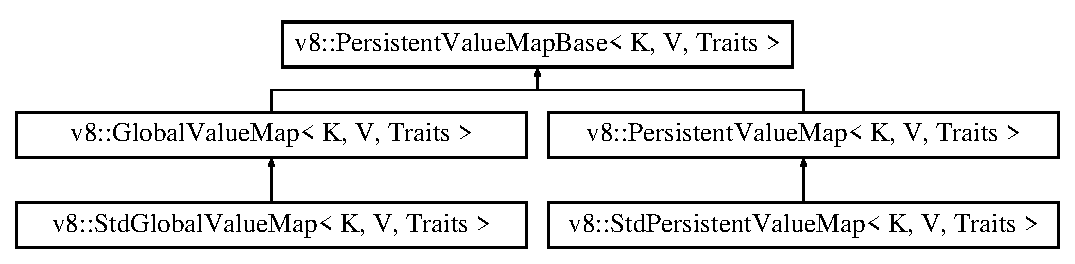
\includegraphics[height=3.000000cm]{classv8_1_1_persistent_value_map_base}
\end{center}
\end{figure}
\subsection*{Classes}
\begin{DoxyCompactItemize}
\item 
class \hyperlink{classv8_1_1_persistent_value_map_base_1_1_persistent_value_reference}{Persistent\+Value\+Reference}
\end{DoxyCompactItemize}
\subsection*{Public Member Functions}
\begin{DoxyCompactItemize}
\item 
\hyperlink{classv8_1_1_isolate}{Isolate} $\ast$ {\bfseries Get\+Isolate} ()\hypertarget{classv8_1_1_persistent_value_map_base_a80da7adc6e8bdb166912075346116978}{}\label{classv8_1_1_persistent_value_map_base_a80da7adc6e8bdb166912075346116978}

\item 
size\+\_\+t \hyperlink{classv8_1_1_persistent_value_map_base_ade5c5db2a968fdabe073649e85b837eb}{Size} ()
\item 
bool \hyperlink{classv8_1_1_persistent_value_map_base_a9f824b13dd30605589508db2740dd678}{Is\+Weak} ()
\item 
\hyperlink{classv8_1_1_local}{Local}$<$ V $>$ \hyperlink{classv8_1_1_persistent_value_map_base_a16b8f906ea42036c2f37d44813bf2a72}{Get} (const K \&key)
\item 
bool \hyperlink{classv8_1_1_persistent_value_map_base_a8c68e5f99c4042541c6d32232c97282a}{Contains} (const K \&key)
\item 
bool \hyperlink{classv8_1_1_persistent_value_map_base_a85201649d2bbd0ffdebe8be3d5c6447a}{Set\+Return\+Value} (const K \&key, \hyperlink{classv8_1_1_return_value}{Return\+Value}$<$ \hyperlink{classv8_1_1_value}{Value} $>$ return\+Value)
\item 
void \hyperlink{classv8_1_1_persistent_value_map_base_a6fa5f720b283dd9fa626a67e7687dcd0}{Set\+Reference} (const K \&key, const \hyperlink{classv8_1_1_persistent}{Persistent}$<$ \hyperlink{classv8_1_1_object}{Object} $>$ \&parent)
\item 
void \hyperlink{classv8_1_1_persistent_value_map_base_a7d1cd63172b997dfaac9d0f009edd709}{Register\+Externally\+Referenced\+Object} (K \&key)
\item 
\hyperlink{classv8_1_1_global}{Global}$<$ V $>$ \hyperlink{classv8_1_1_persistent_value_map_base_abd75a4c050416712167ba0bb9eace097}{Remove} (const K \&key)
\item 
void \hyperlink{classv8_1_1_persistent_value_map_base_a1bf074e7a7c24713c9a3d40ddce89e74}{Clear} ()
\item 
\hyperlink{classv8_1_1_persistent_value_map_base_1_1_persistent_value_reference}{Persistent\+Value\+Reference} \hyperlink{classv8_1_1_persistent_value_map_base_a52e74c69b94c7ce77a65af9f32d68af4}{Get\+Reference} (const K \&key)
\end{DoxyCompactItemize}
\subsection*{Protected Member Functions}
\begin{DoxyCompactItemize}
\item 
{\bfseries Persistent\+Value\+Map\+Base} (\hyperlink{classv8_1_1_isolate}{Isolate} $\ast$isolate)\hypertarget{classv8_1_1_persistent_value_map_base_a1adee3f8b1ff929f07ddf9e94c6108ed}{}\label{classv8_1_1_persistent_value_map_base_a1adee3f8b1ff929f07ddf9e94c6108ed}

\item 
\hyperlink{classv8_1_1_isolate}{Isolate} $\ast$ {\bfseries isolate} ()\hypertarget{classv8_1_1_persistent_value_map_base_af2e83791955c6027213dd979eebeb8f4}{}\label{classv8_1_1_persistent_value_map_base_af2e83791955c6027213dd979eebeb8f4}

\item 
Traits\+::\+Impl $\ast$ {\bfseries impl} ()\hypertarget{classv8_1_1_persistent_value_map_base_aacd576258fbffaf366436a6ecdd8cdf5}{}\label{classv8_1_1_persistent_value_map_base_aacd576258fbffaf366436a6ecdd8cdf5}

\item 
void {\bfseries Remove\+Weak} (const K \&key)\hypertarget{classv8_1_1_persistent_value_map_base_a5c16ace49c257f760c92a010a93b4884}{}\label{classv8_1_1_persistent_value_map_base_a5c16ace49c257f760c92a010a93b4884}

\end{DoxyCompactItemize}
\subsection*{Static Protected Member Functions}
\begin{DoxyCompactItemize}
\item 
static V $\ast$ {\bfseries From\+Val} (Persistent\+Container\+Value v)\hypertarget{classv8_1_1_persistent_value_map_base_af8fcd471f2d53ffca9881f7c436044e8}{}\label{classv8_1_1_persistent_value_map_base_af8fcd471f2d53ffca9881f7c436044e8}

\item 
static Persistent\+Container\+Value {\bfseries Clear\+And\+Leak} (\hyperlink{classv8_1_1_global}{Global}$<$ V $>$ $\ast$persistent)\hypertarget{classv8_1_1_persistent_value_map_base_a7b083c75829bbc4177729ffe9827c4ac}{}\label{classv8_1_1_persistent_value_map_base_a7b083c75829bbc4177729ffe9827c4ac}

\item 
static Persistent\+Container\+Value {\bfseries Leak} (\hyperlink{classv8_1_1_global}{Global}$<$ V $>$ $\ast$persistent)\hypertarget{classv8_1_1_persistent_value_map_base_adacf68ca7b9fb19deab68711a70a8313}{}\label{classv8_1_1_persistent_value_map_base_adacf68ca7b9fb19deab68711a70a8313}

\item 
static \hyperlink{classv8_1_1_global}{Global}$<$ V $>$ \hyperlink{classv8_1_1_persistent_value_map_base_a9ffa7a4e0c59121c0471d71c04112966}{Release} (Persistent\+Container\+Value v)
\end{DoxyCompactItemize}
\subsection*{Private Member Functions}
\begin{DoxyCompactItemize}
\item 
{\bfseries Persistent\+Value\+Map\+Base} (\hyperlink{classv8_1_1_persistent_value_map_base}{Persistent\+Value\+Map\+Base} \&)\hypertarget{classv8_1_1_persistent_value_map_base_af083c2f017cdbd5d11cc26cefd62ee89}{}\label{classv8_1_1_persistent_value_map_base_af083c2f017cdbd5d11cc26cefd62ee89}

\item 
void {\bfseries operator=} (\hyperlink{classv8_1_1_persistent_value_map_base}{Persistent\+Value\+Map\+Base} \&)\hypertarget{classv8_1_1_persistent_value_map_base_ae18eeb1c509804447ddb6dbe18463259}{}\label{classv8_1_1_persistent_value_map_base_ae18eeb1c509804447ddb6dbe18463259}

\end{DoxyCompactItemize}
\subsection*{Static Private Member Functions}
\begin{DoxyCompactItemize}
\item 
static bool {\bfseries Set\+Return\+Value\+From\+Val} (\hyperlink{classv8_1_1_return_value}{Return\+Value}$<$ \hyperlink{classv8_1_1_value}{Value} $>$ $\ast$return\+Value, Persistent\+Container\+Value value)\hypertarget{classv8_1_1_persistent_value_map_base_ade3df16080e354eb430edc1a45e05007}{}\label{classv8_1_1_persistent_value_map_base_ade3df16080e354eb430edc1a45e05007}

\end{DoxyCompactItemize}
\subsection*{Private Attributes}
\begin{DoxyCompactItemize}
\item 
\hyperlink{classv8_1_1_isolate}{Isolate} $\ast$ {\bfseries isolate\+\_\+}\hypertarget{classv8_1_1_persistent_value_map_base_ade71227119d310117c0aefdea1c03ba5}{}\label{classv8_1_1_persistent_value_map_base_ade71227119d310117c0aefdea1c03ba5}

\item 
Traits\+::\+Impl {\bfseries impl\+\_\+}\hypertarget{classv8_1_1_persistent_value_map_base_ab72a180bc12ace83c2b29b711476bf6a}{}\label{classv8_1_1_persistent_value_map_base_ab72a180bc12ace83c2b29b711476bf6a}

\end{DoxyCompactItemize}


\subsection{Detailed Description}
\subsubsection*{template$<$typename K, typename V, typename Traits$>$\\*
class v8\+::\+Persistent\+Value\+Map\+Base$<$ K, V, Traits $>$}

A map wrapper that allows using \hyperlink{classv8_1_1_global}{Global} as a mapped value. C++11 embedders don\textquotesingle{}t need this class, as they can use \hyperlink{classv8_1_1_global}{Global} directly in std containers.

The map relies on a backing map, whose type and accessors are described by the Traits class. The backing map will handle values of type Persistent\+Container\+Value, with all conversion into and out of \hyperlink{classv8_1_1_v8}{V8} handles being transparently handled by this class. 

\subsection{Member Function Documentation}
\index{v8\+::\+Persistent\+Value\+Map\+Base@{v8\+::\+Persistent\+Value\+Map\+Base}!Clear@{Clear}}
\index{Clear@{Clear}!v8\+::\+Persistent\+Value\+Map\+Base@{v8\+::\+Persistent\+Value\+Map\+Base}}
\subsubsection[{\texorpdfstring{Clear()}{Clear()}}]{\setlength{\rightskip}{0pt plus 5cm}template$<$typename K , typename V , typename Traits $>$ void {\bf v8\+::\+Persistent\+Value\+Map\+Base}$<$ K, V, Traits $>$\+::Clear (
\begin{DoxyParamCaption}
{}
\end{DoxyParamCaption}
)\hspace{0.3cm}{\ttfamily [inline]}}\hypertarget{classv8_1_1_persistent_value_map_base_a1bf074e7a7c24713c9a3d40ddce89e74}{}\label{classv8_1_1_persistent_value_map_base_a1bf074e7a7c24713c9a3d40ddce89e74}
Traverses the map repeatedly, in case side effects of disposal cause insertions. \index{v8\+::\+Persistent\+Value\+Map\+Base@{v8\+::\+Persistent\+Value\+Map\+Base}!Contains@{Contains}}
\index{Contains@{Contains}!v8\+::\+Persistent\+Value\+Map\+Base@{v8\+::\+Persistent\+Value\+Map\+Base}}
\subsubsection[{\texorpdfstring{Contains(const K \&key)}{Contains(const K &key)}}]{\setlength{\rightskip}{0pt plus 5cm}template$<$typename K , typename V , typename Traits $>$ bool {\bf v8\+::\+Persistent\+Value\+Map\+Base}$<$ K, V, Traits $>$\+::Contains (
\begin{DoxyParamCaption}
\item[{const K \&}]{key}
\end{DoxyParamCaption}
)\hspace{0.3cm}{\ttfamily [inline]}}\hypertarget{classv8_1_1_persistent_value_map_base_a8c68e5f99c4042541c6d32232c97282a}{}\label{classv8_1_1_persistent_value_map_base_a8c68e5f99c4042541c6d32232c97282a}
Check whether a value is contained in the map. \index{v8\+::\+Persistent\+Value\+Map\+Base@{v8\+::\+Persistent\+Value\+Map\+Base}!Get@{Get}}
\index{Get@{Get}!v8\+::\+Persistent\+Value\+Map\+Base@{v8\+::\+Persistent\+Value\+Map\+Base}}
\subsubsection[{\texorpdfstring{Get(const K \&key)}{Get(const K &key)}}]{\setlength{\rightskip}{0pt plus 5cm}template$<$typename K , typename V , typename Traits $>$ {\bf Local}$<$V$>$ {\bf v8\+::\+Persistent\+Value\+Map\+Base}$<$ K, V, Traits $>$\+::Get (
\begin{DoxyParamCaption}
\item[{const K \&}]{key}
\end{DoxyParamCaption}
)\hspace{0.3cm}{\ttfamily [inline]}}\hypertarget{classv8_1_1_persistent_value_map_base_a16b8f906ea42036c2f37d44813bf2a72}{}\label{classv8_1_1_persistent_value_map_base_a16b8f906ea42036c2f37d44813bf2a72}
Get value stored in map. \index{v8\+::\+Persistent\+Value\+Map\+Base@{v8\+::\+Persistent\+Value\+Map\+Base}!Get\+Reference@{Get\+Reference}}
\index{Get\+Reference@{Get\+Reference}!v8\+::\+Persistent\+Value\+Map\+Base@{v8\+::\+Persistent\+Value\+Map\+Base}}
\subsubsection[{\texorpdfstring{Get\+Reference(const K \&key)}{GetReference(const K &key)}}]{\setlength{\rightskip}{0pt plus 5cm}template$<$typename K , typename V , typename Traits $>$ {\bf Persistent\+Value\+Reference} {\bf v8\+::\+Persistent\+Value\+Map\+Base}$<$ K, V, Traits $>$\+::Get\+Reference (
\begin{DoxyParamCaption}
\item[{const K \&}]{key}
\end{DoxyParamCaption}
)\hspace{0.3cm}{\ttfamily [inline]}}\hypertarget{classv8_1_1_persistent_value_map_base_a52e74c69b94c7ce77a65af9f32d68af4}{}\label{classv8_1_1_persistent_value_map_base_a52e74c69b94c7ce77a65af9f32d68af4}
Get a reference to a map value. This enables fast, repeated access to a value stored in the map while the map remains unchanged.

Careful\+: This is potentially unsafe, so please use with care. The value will become invalid if the value for this key changes in the underlying map, as a result of \hyperlink{classv8_1_1_set}{Set} or Remove for the same key; as a result of the weak callback for the same key; or as a result of calling \hyperlink{classv8_1_1_persistent_value_map_base_a1bf074e7a7c24713c9a3d40ddce89e74}{Clear()} or destruction of the map. \index{v8\+::\+Persistent\+Value\+Map\+Base@{v8\+::\+Persistent\+Value\+Map\+Base}!Is\+Weak@{Is\+Weak}}
\index{Is\+Weak@{Is\+Weak}!v8\+::\+Persistent\+Value\+Map\+Base@{v8\+::\+Persistent\+Value\+Map\+Base}}
\subsubsection[{\texorpdfstring{Is\+Weak()}{IsWeak()}}]{\setlength{\rightskip}{0pt plus 5cm}template$<$typename K , typename V , typename Traits $>$ bool {\bf v8\+::\+Persistent\+Value\+Map\+Base}$<$ K, V, Traits $>$\+::Is\+Weak (
\begin{DoxyParamCaption}
{}
\end{DoxyParamCaption}
)\hspace{0.3cm}{\ttfamily [inline]}}\hypertarget{classv8_1_1_persistent_value_map_base_a9f824b13dd30605589508db2740dd678}{}\label{classv8_1_1_persistent_value_map_base_a9f824b13dd30605589508db2740dd678}
Return whether the map holds weak persistents. \index{v8\+::\+Persistent\+Value\+Map\+Base@{v8\+::\+Persistent\+Value\+Map\+Base}!Register\+Externally\+Referenced\+Object@{Register\+Externally\+Referenced\+Object}}
\index{Register\+Externally\+Referenced\+Object@{Register\+Externally\+Referenced\+Object}!v8\+::\+Persistent\+Value\+Map\+Base@{v8\+::\+Persistent\+Value\+Map\+Base}}
\subsubsection[{\texorpdfstring{Register\+Externally\+Referenced\+Object(\+K \&key)}{RegisterExternallyReferencedObject(K &key)}}]{\setlength{\rightskip}{0pt plus 5cm}template$<$typename K , typename V , typename Traits $>$ void {\bf v8\+::\+Persistent\+Value\+Map\+Base}$<$ K, V, Traits $>$\+::Register\+Externally\+Referenced\+Object (
\begin{DoxyParamCaption}
\item[{K \&}]{key}
\end{DoxyParamCaption}
)\hspace{0.3cm}{\ttfamily [inline]}}\hypertarget{classv8_1_1_persistent_value_map_base_a7d1cd63172b997dfaac9d0f009edd709}{}\label{classv8_1_1_persistent_value_map_base_a7d1cd63172b997dfaac9d0f009edd709}
Call V8\+::\+Register\+Externally\+Referenced\+Object with the map value for given key. \index{v8\+::\+Persistent\+Value\+Map\+Base@{v8\+::\+Persistent\+Value\+Map\+Base}!Release@{Release}}
\index{Release@{Release}!v8\+::\+Persistent\+Value\+Map\+Base@{v8\+::\+Persistent\+Value\+Map\+Base}}
\subsubsection[{\texorpdfstring{Release(\+Persistent\+Container\+Value v)}{Release(PersistentContainerValue v)}}]{\setlength{\rightskip}{0pt plus 5cm}template$<$typename K , typename V , typename Traits $>$ static {\bf Global}$<$V$>$ {\bf v8\+::\+Persistent\+Value\+Map\+Base}$<$ K, V, Traits $>$\+::Release (
\begin{DoxyParamCaption}
\item[{Persistent\+Container\+Value}]{v}
\end{DoxyParamCaption}
)\hspace{0.3cm}{\ttfamily [inline]}, {\ttfamily [static]}, {\ttfamily [protected]}}\hypertarget{classv8_1_1_persistent_value_map_base_a9ffa7a4e0c59121c0471d71c04112966}{}\label{classv8_1_1_persistent_value_map_base_a9ffa7a4e0c59121c0471d71c04112966}
Return a container value as \hyperlink{classv8_1_1_global}{Global} and make sure the weak callback is properly disposed of. All remove functionality should go through this. \index{v8\+::\+Persistent\+Value\+Map\+Base@{v8\+::\+Persistent\+Value\+Map\+Base}!Remove@{Remove}}
\index{Remove@{Remove}!v8\+::\+Persistent\+Value\+Map\+Base@{v8\+::\+Persistent\+Value\+Map\+Base}}
\subsubsection[{\texorpdfstring{Remove(const K \&key)}{Remove(const K &key)}}]{\setlength{\rightskip}{0pt plus 5cm}template$<$typename K , typename V , typename Traits $>$ {\bf Global}$<$V$>$ {\bf v8\+::\+Persistent\+Value\+Map\+Base}$<$ K, V, Traits $>$\+::Remove (
\begin{DoxyParamCaption}
\item[{const K \&}]{key}
\end{DoxyParamCaption}
)\hspace{0.3cm}{\ttfamily [inline]}}\hypertarget{classv8_1_1_persistent_value_map_base_abd75a4c050416712167ba0bb9eace097}{}\label{classv8_1_1_persistent_value_map_base_abd75a4c050416712167ba0bb9eace097}
Return value for key and remove it from the map. \index{v8\+::\+Persistent\+Value\+Map\+Base@{v8\+::\+Persistent\+Value\+Map\+Base}!Set\+Reference@{Set\+Reference}}
\index{Set\+Reference@{Set\+Reference}!v8\+::\+Persistent\+Value\+Map\+Base@{v8\+::\+Persistent\+Value\+Map\+Base}}
\subsubsection[{\texorpdfstring{Set\+Reference(const K \&key, const Persistent$<$ Object $>$ \&parent)}{SetReference(const K &key, const Persistent< Object > &parent)}}]{\setlength{\rightskip}{0pt plus 5cm}template$<$typename K , typename V , typename Traits $>$ void {\bf v8\+::\+Persistent\+Value\+Map\+Base}$<$ K, V, Traits $>$\+::Set\+Reference (
\begin{DoxyParamCaption}
\item[{const K \&}]{key, }
\item[{const {\bf Persistent}$<$ {\bf Object} $>$ \&}]{parent}
\end{DoxyParamCaption}
)\hspace{0.3cm}{\ttfamily [inline]}}\hypertarget{classv8_1_1_persistent_value_map_base_a6fa5f720b283dd9fa626a67e7687dcd0}{}\label{classv8_1_1_persistent_value_map_base_a6fa5f720b283dd9fa626a67e7687dcd0}
Call \hyperlink{classv8_1_1_isolate_a055fc73d18747b96c51f00599cdd3ec1}{Isolate\+::\+Set\+Reference} with the given parent and the map value. \index{v8\+::\+Persistent\+Value\+Map\+Base@{v8\+::\+Persistent\+Value\+Map\+Base}!Set\+Return\+Value@{Set\+Return\+Value}}
\index{Set\+Return\+Value@{Set\+Return\+Value}!v8\+::\+Persistent\+Value\+Map\+Base@{v8\+::\+Persistent\+Value\+Map\+Base}}
\subsubsection[{\texorpdfstring{Set\+Return\+Value(const K \&key, Return\+Value$<$ Value $>$ return\+Value)}{SetReturnValue(const K &key, ReturnValue< Value > returnValue)}}]{\setlength{\rightskip}{0pt plus 5cm}template$<$typename K , typename V , typename Traits $>$ bool {\bf v8\+::\+Persistent\+Value\+Map\+Base}$<$ K, V, Traits $>$\+::Set\+Return\+Value (
\begin{DoxyParamCaption}
\item[{const K \&}]{key, }
\item[{{\bf Return\+Value}$<$ {\bf Value} $>$}]{return\+Value}
\end{DoxyParamCaption}
)\hspace{0.3cm}{\ttfamily [inline]}}\hypertarget{classv8_1_1_persistent_value_map_base_a85201649d2bbd0ffdebe8be3d5c6447a}{}\label{classv8_1_1_persistent_value_map_base_a85201649d2bbd0ffdebe8be3d5c6447a}
Get value stored in map and set it in return\+Value. Return true if a value was found. \index{v8\+::\+Persistent\+Value\+Map\+Base@{v8\+::\+Persistent\+Value\+Map\+Base}!Size@{Size}}
\index{Size@{Size}!v8\+::\+Persistent\+Value\+Map\+Base@{v8\+::\+Persistent\+Value\+Map\+Base}}
\subsubsection[{\texorpdfstring{Size()}{Size()}}]{\setlength{\rightskip}{0pt plus 5cm}template$<$typename K , typename V , typename Traits $>$ size\+\_\+t {\bf v8\+::\+Persistent\+Value\+Map\+Base}$<$ K, V, Traits $>$\+::Size (
\begin{DoxyParamCaption}
{}
\end{DoxyParamCaption}
)\hspace{0.3cm}{\ttfamily [inline]}}\hypertarget{classv8_1_1_persistent_value_map_base_ade5c5db2a968fdabe073649e85b837eb}{}\label{classv8_1_1_persistent_value_map_base_ade5c5db2a968fdabe073649e85b837eb}
Return size of the map. 

The documentation for this class was generated from the following file\+:\begin{DoxyCompactItemize}
\item 
/\+Users/joshgav/node/v8/include/v8-\/util.\+h\end{DoxyCompactItemize}

\hypertarget{classv8_1_1_persistent_value_map_base_1_1_persistent_value_reference}{}\section{v8\+:\+:Persistent\+Value\+Map\+Base$<$ K, V, Traits $>$\+:\+:Persistent\+Value\+Reference Class Reference}
\label{classv8_1_1_persistent_value_map_base_1_1_persistent_value_reference}\index{v8\+::\+Persistent\+Value\+Map\+Base$<$ K, V, Traits $>$\+::\+Persistent\+Value\+Reference@{v8\+::\+Persistent\+Value\+Map\+Base$<$ K, V, Traits $>$\+::\+Persistent\+Value\+Reference}}


{\ttfamily \#include $<$v8-\/util.\+h$>$}

\subsection*{Public Member Functions}
\begin{DoxyCompactItemize}
\item 
{\bfseries Persistent\+Value\+Reference} (const \hyperlink{classv8_1_1_persistent_value_map_base_1_1_persistent_value_reference}{Persistent\+Value\+Reference} \&other)\hypertarget{classv8_1_1_persistent_value_map_base_1_1_persistent_value_reference_a47103822e6717eb42de116ddc773e334}{}\label{classv8_1_1_persistent_value_map_base_1_1_persistent_value_reference_a47103822e6717eb42de116ddc773e334}

\item 
\hyperlink{classv8_1_1_local}{Local}$<$ V $>$ {\bfseries New\+Local} (\hyperlink{classv8_1_1_isolate}{Isolate} $\ast$isolate) const \hypertarget{classv8_1_1_persistent_value_map_base_1_1_persistent_value_reference_a714a3ff6ea3e196bdb2ec244adf39e5f}{}\label{classv8_1_1_persistent_value_map_base_1_1_persistent_value_reference_a714a3ff6ea3e196bdb2ec244adf39e5f}

\item 
bool {\bfseries Is\+Empty} () const \hypertarget{classv8_1_1_persistent_value_map_base_1_1_persistent_value_reference_a39e28fe15080e676039deeaf7a8e57b5}{}\label{classv8_1_1_persistent_value_map_base_1_1_persistent_value_reference_a39e28fe15080e676039deeaf7a8e57b5}

\item 
{\footnotesize template$<$typename T $>$ }\\bool {\bfseries Set\+Return\+Value} (\hyperlink{classv8_1_1_return_value}{Return\+Value}$<$ T $>$ return\+Value)\hypertarget{classv8_1_1_persistent_value_map_base_1_1_persistent_value_reference_a4003b2d7d0f3cc84574d2e74a1713f27}{}\label{classv8_1_1_persistent_value_map_base_1_1_persistent_value_reference_a4003b2d7d0f3cc84574d2e74a1713f27}

\item 
void {\bfseries Reset} ()\hypertarget{classv8_1_1_persistent_value_map_base_1_1_persistent_value_reference_a94c91d959beb24cad37458b2ae43a97b}{}\label{classv8_1_1_persistent_value_map_base_1_1_persistent_value_reference_a94c91d959beb24cad37458b2ae43a97b}

\item 
void {\bfseries operator=} (const \hyperlink{classv8_1_1_persistent_value_map_base_1_1_persistent_value_reference}{Persistent\+Value\+Reference} \&other)\hypertarget{classv8_1_1_persistent_value_map_base_1_1_persistent_value_reference_abcbf6c9229d0b322c64fe5110726c421}{}\label{classv8_1_1_persistent_value_map_base_1_1_persistent_value_reference_abcbf6c9229d0b322c64fe5110726c421}

\end{DoxyCompactItemize}
\subsection*{Private Member Functions}
\begin{DoxyCompactItemize}
\item 
{\bfseries Persistent\+Value\+Reference} (Persistent\+Container\+Value value)\hypertarget{classv8_1_1_persistent_value_map_base_1_1_persistent_value_reference_a0d7469174626cee27afd20846138498d}{}\label{classv8_1_1_persistent_value_map_base_1_1_persistent_value_reference_a0d7469174626cee27afd20846138498d}

\item 
void {\bfseries operator=} (Persistent\+Container\+Value value)\hypertarget{classv8_1_1_persistent_value_map_base_1_1_persistent_value_reference_a521345ca3a629265494faf81d0630750}{}\label{classv8_1_1_persistent_value_map_base_1_1_persistent_value_reference_a521345ca3a629265494faf81d0630750}

\end{DoxyCompactItemize}
\subsection*{Private Attributes}
\begin{DoxyCompactItemize}
\item 
Persistent\+Container\+Value {\bfseries value\+\_\+}\hypertarget{classv8_1_1_persistent_value_map_base_1_1_persistent_value_reference_adb5f76de4ed5468b9cce738625a7e3e0}{}\label{classv8_1_1_persistent_value_map_base_1_1_persistent_value_reference_adb5f76de4ed5468b9cce738625a7e3e0}

\end{DoxyCompactItemize}
\subsection*{Friends}
\begin{DoxyCompactItemize}
\item 
class {\bfseries Persistent\+Value\+Map\+Base}\hypertarget{classv8_1_1_persistent_value_map_base_1_1_persistent_value_reference_ae5cccd63ef6d94c509ad8b6970d4017d}{}\label{classv8_1_1_persistent_value_map_base_1_1_persistent_value_reference_ae5cccd63ef6d94c509ad8b6970d4017d}

\item 
class {\bfseries Persistent\+Value\+Map$<$ K, V, Traits $>$}\hypertarget{classv8_1_1_persistent_value_map_base_1_1_persistent_value_reference_a22fcaa9f3ba179f3bb566eda5b93790d}{}\label{classv8_1_1_persistent_value_map_base_1_1_persistent_value_reference_a22fcaa9f3ba179f3bb566eda5b93790d}

\item 
class {\bfseries Global\+Value\+Map$<$ K, V, Traits $>$}\hypertarget{classv8_1_1_persistent_value_map_base_1_1_persistent_value_reference_a41811cde55d1ef227d1ba28778d95d08}{}\label{classv8_1_1_persistent_value_map_base_1_1_persistent_value_reference_a41811cde55d1ef227d1ba28778d95d08}

\end{DoxyCompactItemize}


\subsection{Detailed Description}
\subsubsection*{template$<$typename K, typename V, typename Traits$>$\\*
class v8\+::\+Persistent\+Value\+Map\+Base$<$ K, V, Traits $>$\+::\+Persistent\+Value\+Reference}

Helper class for Get\+Reference/\+Set\+With\+Reference. Do not use outside that context. 

The documentation for this class was generated from the following file\+:\begin{DoxyCompactItemize}
\item 
/\+Users/joshgav/node/v8/include/v8-\/util.\+h\end{DoxyCompactItemize}

\hypertarget{classv8_1_1_persistent_value_vector}{}\section{v8\+:\+:Persistent\+Value\+Vector$<$ V, Traits $>$ Class Template Reference}
\label{classv8_1_1_persistent_value_vector}\index{v8\+::\+Persistent\+Value\+Vector$<$ V, Traits $>$@{v8\+::\+Persistent\+Value\+Vector$<$ V, Traits $>$}}


{\ttfamily \#include $<$v8-\/util.\+h$>$}

\subsection*{Public Member Functions}
\begin{DoxyCompactItemize}
\item 
{\bfseries Persistent\+Value\+Vector} (\hyperlink{classv8_1_1_isolate}{Isolate} $\ast$isolate)\hypertarget{classv8_1_1_persistent_value_vector_ab6b9994133c30359ad7a02d3cc05219c}{}\label{classv8_1_1_persistent_value_vector_ab6b9994133c30359ad7a02d3cc05219c}

\item 
void \hyperlink{classv8_1_1_persistent_value_vector_a02376c6d16be29084db46f65473477fb}{Append} (\hyperlink{classv8_1_1_local}{Local}$<$ V $>$ value)
\item 
void \hyperlink{classv8_1_1_persistent_value_vector_ad076923fd0046196670e87e996582546}{Append} (\hyperlink{classv8_1_1_global}{Global}$<$ V $>$ persistent)
\item 
bool \hyperlink{classv8_1_1_persistent_value_vector_a9ad869bc3f60fc227fecf202b36b650a}{Is\+Empty} () const 
\item 
size\+\_\+t \hyperlink{classv8_1_1_persistent_value_vector_a0e152d147a2553746e56cbf9e6311506}{Size} () const 
\item 
\hyperlink{classv8_1_1_local}{Local}$<$ V $>$ \hyperlink{classv8_1_1_persistent_value_vector_a7b47cacf60ddfa3e2a7f57d788f18b84}{Get} (size\+\_\+t index) const 
\item 
void \hyperlink{classv8_1_1_persistent_value_vector_ad07f449c2004b4f3d91e58cabde99a53}{Clear} ()
\item 
void \hyperlink{classv8_1_1_persistent_value_vector_ad4cccfee3a275986578276efe0c78510}{Reserve\+Capacity} (size\+\_\+t capacity)
\end{DoxyCompactItemize}
\subsection*{Static Private Member Functions}
\begin{DoxyCompactItemize}
\item 
static Persistent\+Container\+Value {\bfseries Clear\+And\+Leak} (\hyperlink{classv8_1_1_global}{Global}$<$ V $>$ $\ast$persistent)\hypertarget{classv8_1_1_persistent_value_vector_a17d319e9935cb951900cbcf869c596d5}{}\label{classv8_1_1_persistent_value_vector_a17d319e9935cb951900cbcf869c596d5}

\item 
static V $\ast$ {\bfseries From\+Val} (Persistent\+Container\+Value v)\hypertarget{classv8_1_1_persistent_value_vector_a8ee50e074674ca91a3dc2370f1ddbf06}{}\label{classv8_1_1_persistent_value_vector_a8ee50e074674ca91a3dc2370f1ddbf06}

\end{DoxyCompactItemize}
\subsection*{Private Attributes}
\begin{DoxyCompactItemize}
\item 
\hyperlink{classv8_1_1_isolate}{Isolate} $\ast$ {\bfseries isolate\+\_\+}\hypertarget{classv8_1_1_persistent_value_vector_a8d7f3de6fa62cfaff370b2bdf72c638b}{}\label{classv8_1_1_persistent_value_vector_a8d7f3de6fa62cfaff370b2bdf72c638b}

\item 
Traits\+::\+Impl {\bfseries impl\+\_\+}\hypertarget{classv8_1_1_persistent_value_vector_ae6bad422949b86010a4c8791bb912eec}{}\label{classv8_1_1_persistent_value_vector_ae6bad422949b86010a4c8791bb912eec}

\end{DoxyCompactItemize}


\subsection{Detailed Description}
\subsubsection*{template$<$typename V, typename Traits = Default\+Persistent\+Value\+Vector\+Traits$>$\\*
class v8\+::\+Persistent\+Value\+Vector$<$ V, Traits $>$}

A vector wrapper that safely stores \hyperlink{classv8_1_1_global}{Global} values. C++11 embedders don\textquotesingle{}t need this class, as they can use \hyperlink{classv8_1_1_global}{Global} directly in std containers.

This class relies on a backing vector implementation, whose type and methods are described by the Traits class. The backing map will handle values of type Persistent\+Container\+Value, with all conversion into and out of \hyperlink{classv8_1_1_v8}{V8} handles being transparently handled by this class. 

\subsection{Member Function Documentation}
\index{v8\+::\+Persistent\+Value\+Vector@{v8\+::\+Persistent\+Value\+Vector}!Append@{Append}}
\index{Append@{Append}!v8\+::\+Persistent\+Value\+Vector@{v8\+::\+Persistent\+Value\+Vector}}
\subsubsection[{\texorpdfstring{Append(\+Local$<$ V $>$ value)}{Append(Local< V > value)}}]{\setlength{\rightskip}{0pt plus 5cm}template$<$typename V , typename Traits  = Default\+Persistent\+Value\+Vector\+Traits$>$ void {\bf v8\+::\+Persistent\+Value\+Vector}$<$ V, Traits $>$\+::Append (
\begin{DoxyParamCaption}
\item[{{\bf Local}$<$ V $>$}]{value}
\end{DoxyParamCaption}
)\hspace{0.3cm}{\ttfamily [inline]}}\hypertarget{classv8_1_1_persistent_value_vector_a02376c6d16be29084db46f65473477fb}{}\label{classv8_1_1_persistent_value_vector_a02376c6d16be29084db46f65473477fb}
Append a value to the vector. \index{v8\+::\+Persistent\+Value\+Vector@{v8\+::\+Persistent\+Value\+Vector}!Append@{Append}}
\index{Append@{Append}!v8\+::\+Persistent\+Value\+Vector@{v8\+::\+Persistent\+Value\+Vector}}
\subsubsection[{\texorpdfstring{Append(\+Global$<$ V $>$ persistent)}{Append(Global< V > persistent)}}]{\setlength{\rightskip}{0pt plus 5cm}template$<$typename V , typename Traits  = Default\+Persistent\+Value\+Vector\+Traits$>$ void {\bf v8\+::\+Persistent\+Value\+Vector}$<$ V, Traits $>$\+::Append (
\begin{DoxyParamCaption}
\item[{{\bf Global}$<$ V $>$}]{persistent}
\end{DoxyParamCaption}
)\hspace{0.3cm}{\ttfamily [inline]}}\hypertarget{classv8_1_1_persistent_value_vector_ad076923fd0046196670e87e996582546}{}\label{classv8_1_1_persistent_value_vector_ad076923fd0046196670e87e996582546}
Append a persistent\textquotesingle{}s value to the vector. \index{v8\+::\+Persistent\+Value\+Vector@{v8\+::\+Persistent\+Value\+Vector}!Clear@{Clear}}
\index{Clear@{Clear}!v8\+::\+Persistent\+Value\+Vector@{v8\+::\+Persistent\+Value\+Vector}}
\subsubsection[{\texorpdfstring{Clear()}{Clear()}}]{\setlength{\rightskip}{0pt plus 5cm}template$<$typename V , typename Traits  = Default\+Persistent\+Value\+Vector\+Traits$>$ void {\bf v8\+::\+Persistent\+Value\+Vector}$<$ V, Traits $>$\+::Clear (
\begin{DoxyParamCaption}
{}
\end{DoxyParamCaption}
)\hspace{0.3cm}{\ttfamily [inline]}}\hypertarget{classv8_1_1_persistent_value_vector_ad07f449c2004b4f3d91e58cabde99a53}{}\label{classv8_1_1_persistent_value_vector_ad07f449c2004b4f3d91e58cabde99a53}
Remove all elements from the vector. \index{v8\+::\+Persistent\+Value\+Vector@{v8\+::\+Persistent\+Value\+Vector}!Get@{Get}}
\index{Get@{Get}!v8\+::\+Persistent\+Value\+Vector@{v8\+::\+Persistent\+Value\+Vector}}
\subsubsection[{\texorpdfstring{Get(size\+\_\+t index) const }{Get(size_t index) const }}]{\setlength{\rightskip}{0pt plus 5cm}template$<$typename V , typename Traits  = Default\+Persistent\+Value\+Vector\+Traits$>$ {\bf Local}$<$V$>$ {\bf v8\+::\+Persistent\+Value\+Vector}$<$ V, Traits $>$\+::Get (
\begin{DoxyParamCaption}
\item[{size\+\_\+t}]{index}
\end{DoxyParamCaption}
) const\hspace{0.3cm}{\ttfamily [inline]}}\hypertarget{classv8_1_1_persistent_value_vector_a7b47cacf60ddfa3e2a7f57d788f18b84}{}\label{classv8_1_1_persistent_value_vector_a7b47cacf60ddfa3e2a7f57d788f18b84}
Retrieve the i-\/th value in the vector. \index{v8\+::\+Persistent\+Value\+Vector@{v8\+::\+Persistent\+Value\+Vector}!Is\+Empty@{Is\+Empty}}
\index{Is\+Empty@{Is\+Empty}!v8\+::\+Persistent\+Value\+Vector@{v8\+::\+Persistent\+Value\+Vector}}
\subsubsection[{\texorpdfstring{Is\+Empty() const }{IsEmpty() const }}]{\setlength{\rightskip}{0pt plus 5cm}template$<$typename V , typename Traits  = Default\+Persistent\+Value\+Vector\+Traits$>$ bool {\bf v8\+::\+Persistent\+Value\+Vector}$<$ V, Traits $>$\+::Is\+Empty (
\begin{DoxyParamCaption}
{}
\end{DoxyParamCaption}
) const\hspace{0.3cm}{\ttfamily [inline]}}\hypertarget{classv8_1_1_persistent_value_vector_a9ad869bc3f60fc227fecf202b36b650a}{}\label{classv8_1_1_persistent_value_vector_a9ad869bc3f60fc227fecf202b36b650a}
Are there any values in the vector? \index{v8\+::\+Persistent\+Value\+Vector@{v8\+::\+Persistent\+Value\+Vector}!Reserve\+Capacity@{Reserve\+Capacity}}
\index{Reserve\+Capacity@{Reserve\+Capacity}!v8\+::\+Persistent\+Value\+Vector@{v8\+::\+Persistent\+Value\+Vector}}
\subsubsection[{\texorpdfstring{Reserve\+Capacity(size\+\_\+t capacity)}{ReserveCapacity(size_t capacity)}}]{\setlength{\rightskip}{0pt plus 5cm}template$<$typename V , typename Traits  = Default\+Persistent\+Value\+Vector\+Traits$>$ void {\bf v8\+::\+Persistent\+Value\+Vector}$<$ V, Traits $>$\+::Reserve\+Capacity (
\begin{DoxyParamCaption}
\item[{size\+\_\+t}]{capacity}
\end{DoxyParamCaption}
)\hspace{0.3cm}{\ttfamily [inline]}}\hypertarget{classv8_1_1_persistent_value_vector_ad4cccfee3a275986578276efe0c78510}{}\label{classv8_1_1_persistent_value_vector_ad4cccfee3a275986578276efe0c78510}
Reserve capacity in the vector. (Efficiency gains depend on the backing implementation.) \index{v8\+::\+Persistent\+Value\+Vector@{v8\+::\+Persistent\+Value\+Vector}!Size@{Size}}
\index{Size@{Size}!v8\+::\+Persistent\+Value\+Vector@{v8\+::\+Persistent\+Value\+Vector}}
\subsubsection[{\texorpdfstring{Size() const }{Size() const }}]{\setlength{\rightskip}{0pt plus 5cm}template$<$typename V , typename Traits  = Default\+Persistent\+Value\+Vector\+Traits$>$ size\+\_\+t {\bf v8\+::\+Persistent\+Value\+Vector}$<$ V, Traits $>$\+::Size (
\begin{DoxyParamCaption}
{}
\end{DoxyParamCaption}
) const\hspace{0.3cm}{\ttfamily [inline]}}\hypertarget{classv8_1_1_persistent_value_vector_a0e152d147a2553746e56cbf9e6311506}{}\label{classv8_1_1_persistent_value_vector_a0e152d147a2553746e56cbf9e6311506}
How many elements are in the vector? 

The documentation for this class was generated from the following file\+:\begin{DoxyCompactItemize}
\item 
/\+Users/joshgav/node/v8/include/v8-\/util.\+h\end{DoxyCompactItemize}

\hypertarget{classv8_1_1_platform}{}\section{v8\+:\+:Platform Class Reference}
\label{classv8_1_1_platform}\index{v8\+::\+Platform@{v8\+::\+Platform}}


{\ttfamily \#include $<$v8-\/platform.\+h$>$}

\subsection*{Public Types}
\begin{DoxyCompactItemize}
\item 
enum \hyperlink{classv8_1_1_platform_ace7f666b2b5995bb0e898e12fa660718}{Expected\+Runtime} \{ \\*
{\bfseries k\+Short\+Running\+Task}, 
\\*
{\bfseries k\+Long\+Running\+Task}
 \}
\end{DoxyCompactItemize}
\subsection*{Public Member Functions}
\begin{DoxyCompactItemize}
\item 
virtual size\+\_\+t \hyperlink{classv8_1_1_platform_a15886ccf5a6a085a2192b305709a527c}{Number\+Of\+Available\+Background\+Threads} ()
\item 
virtual void \hyperlink{classv8_1_1_platform_aa715e6839c1954b4e23b9d2df00bd3ea}{Call\+On\+Background\+Thread} (\hyperlink{classv8_1_1_task}{Task} $\ast$task, \hyperlink{classv8_1_1_platform_ace7f666b2b5995bb0e898e12fa660718}{Expected\+Runtime} expected\+\_\+runtime)=0
\item 
virtual void \hyperlink{classv8_1_1_platform_a8fa13959f919d1d3ff170bceea939915}{Call\+On\+Foreground\+Thread} (\hyperlink{classv8_1_1_isolate}{Isolate} $\ast$isolate, \hyperlink{classv8_1_1_task}{Task} $\ast$task)=0
\item 
virtual void \hyperlink{classv8_1_1_platform_a72bff12d95fbf2118279b0e8f53f8a4b}{Call\+Delayed\+On\+Foreground\+Thread} (\hyperlink{classv8_1_1_isolate}{Isolate} $\ast$isolate, \hyperlink{classv8_1_1_task}{Task} $\ast$task, double delay\+\_\+in\+\_\+seconds)=0
\item 
virtual void \hyperlink{classv8_1_1_platform_ae495999016432391f04d323452084b12}{Call\+Idle\+On\+Foreground\+Thread} (\hyperlink{classv8_1_1_isolate}{Isolate} $\ast$isolate, \hyperlink{classv8_1_1_idle_task}{Idle\+Task} $\ast$task)
\item 
virtual bool \hyperlink{classv8_1_1_platform_ad229642bf16a066d2e8d866dc128141e}{Idle\+Tasks\+Enabled} (\hyperlink{classv8_1_1_isolate}{Isolate} $\ast$isolate)
\item 
virtual double \hyperlink{classv8_1_1_platform_a6d4d7c2dcf6b0c7113099b97fa7f57b7}{Monotonically\+Increasing\+Time} ()=0
\item 
virtual const uint8\+\_\+t $\ast$ \hyperlink{classv8_1_1_platform_a5b81982481986c80d3f613dde54494da}{Get\+Category\+Group\+Enabled} (const char $\ast$name)
\item 
virtual const char $\ast$ \hyperlink{classv8_1_1_platform_a02dde4138b387f1ae2b53190cdac2afc}{Get\+Category\+Group\+Name} (const uint8\+\_\+t $\ast$category\+\_\+enabled\+\_\+flag)
\item 
virtual uint64\+\_\+t \hyperlink{classv8_1_1_platform_ab4ef5713fb5bec0f2fe0981745342364}{Add\+Trace\+Event} (char phase, const uint8\+\_\+t $\ast$category\+\_\+enabled\+\_\+flag, const char $\ast$name, const char $\ast$scope, uint64\+\_\+t id, uint64\+\_\+t bind\+\_\+id, int32\+\_\+t num\+\_\+args, const char $\ast$$\ast$arg\+\_\+names, const uint8\+\_\+t $\ast$arg\+\_\+types, const uint64\+\_\+t $\ast$arg\+\_\+values, unsigned int flags)
\item 
virtual void \hyperlink{classv8_1_1_platform_aa7ead571c0b19687635a930d9c67b73b}{Update\+Trace\+Event\+Duration} (const uint8\+\_\+t $\ast$category\+\_\+enabled\+\_\+flag, const char $\ast$name, uint64\+\_\+t handle)
\end{DoxyCompactItemize}


\subsection{Detailed Description}
\hyperlink{classv8_1_1_v8}{V8} \hyperlink{classv8_1_1_platform}{Platform} abstraction layer.

The embedder has to provide an implementation of this interface before initializing the rest of \hyperlink{classv8_1_1_v8}{V8}. 

\subsection{Member Enumeration Documentation}
\index{v8\+::\+Platform@{v8\+::\+Platform}!Expected\+Runtime@{Expected\+Runtime}}
\index{Expected\+Runtime@{Expected\+Runtime}!v8\+::\+Platform@{v8\+::\+Platform}}
\subsubsection[{\texorpdfstring{Expected\+Runtime}{ExpectedRuntime}}]{\setlength{\rightskip}{0pt plus 5cm}enum {\bf v8\+::\+Platform\+::\+Expected\+Runtime}}\hypertarget{classv8_1_1_platform_ace7f666b2b5995bb0e898e12fa660718}{}\label{classv8_1_1_platform_ace7f666b2b5995bb0e898e12fa660718}
This enum is used to indicate whether a task is potentially long running, or causes a long wait. The embedder might want to use this hint to decide whether to execute the task on a dedicated thread. 

\subsection{Member Function Documentation}
\index{v8\+::\+Platform@{v8\+::\+Platform}!Add\+Trace\+Event@{Add\+Trace\+Event}}
\index{Add\+Trace\+Event@{Add\+Trace\+Event}!v8\+::\+Platform@{v8\+::\+Platform}}
\subsubsection[{\texorpdfstring{Add\+Trace\+Event(char phase, const uint8\+\_\+t $\ast$category\+\_\+enabled\+\_\+flag, const char $\ast$name, const char $\ast$scope, uint64\+\_\+t id, uint64\+\_\+t bind\+\_\+id, int32\+\_\+t num\+\_\+args, const char $\ast$$\ast$arg\+\_\+names, const uint8\+\_\+t $\ast$arg\+\_\+types, const uint64\+\_\+t $\ast$arg\+\_\+values, unsigned int flags)}{AddTraceEvent(char phase, const uint8_t *category_enabled_flag, const char *name, const char *scope, uint64_t id, uint64_t bind_id, int32_t num_args, const char **arg_names, const uint8_t *arg_types, const uint64_t *arg_values, unsigned int flags)}}]{\setlength{\rightskip}{0pt plus 5cm}virtual uint64\+\_\+t v8\+::\+Platform\+::\+Add\+Trace\+Event (
\begin{DoxyParamCaption}
\item[{char}]{phase, }
\item[{const uint8\+\_\+t $\ast$}]{category\+\_\+enabled\+\_\+flag, }
\item[{const char $\ast$}]{name, }
\item[{const char $\ast$}]{scope, }
\item[{uint64\+\_\+t}]{id, }
\item[{uint64\+\_\+t}]{bind\+\_\+id, }
\item[{int32\+\_\+t}]{num\+\_\+args, }
\item[{const char $\ast$$\ast$}]{arg\+\_\+names, }
\item[{const uint8\+\_\+t $\ast$}]{arg\+\_\+types, }
\item[{const uint64\+\_\+t $\ast$}]{arg\+\_\+values, }
\item[{unsigned int}]{flags}
\end{DoxyParamCaption}
)\hspace{0.3cm}{\ttfamily [inline]}, {\ttfamily [virtual]}}\hypertarget{classv8_1_1_platform_ab4ef5713fb5bec0f2fe0981745342364}{}\label{classv8_1_1_platform_ab4ef5713fb5bec0f2fe0981745342364}
Adds a trace event to the platform tracing system. This function call is usually the result of a T\+R\+A\+C\+E\+\_\+$\ast$ macro from trace\+\_\+event\+\_\+common.\+h when tracing and the category of the particular trace are enabled. It is not advisable to call this function on its own; it is really only meant to be used by the trace macros. The returned handle can be used by Update\+Trace\+Event\+Duration to update the duration of C\+O\+M\+P\+L\+E\+TE events. \index{v8\+::\+Platform@{v8\+::\+Platform}!Call\+Delayed\+On\+Foreground\+Thread@{Call\+Delayed\+On\+Foreground\+Thread}}
\index{Call\+Delayed\+On\+Foreground\+Thread@{Call\+Delayed\+On\+Foreground\+Thread}!v8\+::\+Platform@{v8\+::\+Platform}}
\subsubsection[{\texorpdfstring{Call\+Delayed\+On\+Foreground\+Thread(\+Isolate $\ast$isolate, Task $\ast$task, double delay\+\_\+in\+\_\+seconds)=0}{CallDelayedOnForegroundThread(Isolate *isolate, Task *task, double delay_in_seconds)=0}}]{\setlength{\rightskip}{0pt plus 5cm}virtual void v8\+::\+Platform\+::\+Call\+Delayed\+On\+Foreground\+Thread (
\begin{DoxyParamCaption}
\item[{{\bf Isolate} $\ast$}]{isolate, }
\item[{{\bf Task} $\ast$}]{task, }
\item[{double}]{delay\+\_\+in\+\_\+seconds}
\end{DoxyParamCaption}
)\hspace{0.3cm}{\ttfamily [pure virtual]}}\hypertarget{classv8_1_1_platform_a72bff12d95fbf2118279b0e8f53f8a4b}{}\label{classv8_1_1_platform_a72bff12d95fbf2118279b0e8f53f8a4b}
Schedules a task to be invoked on a foreground thread wrt a specific $\vert$isolate$\vert$ after the given number of seconds $\vert$delay\+\_\+in\+\_\+seconds$\vert$. Tasks posted for the same isolate should be execute in order of scheduling. The definition of \char`\"{}foreground\char`\"{} is opaque to \hyperlink{classv8_1_1_v8}{V8}. \index{v8\+::\+Platform@{v8\+::\+Platform}!Call\+Idle\+On\+Foreground\+Thread@{Call\+Idle\+On\+Foreground\+Thread}}
\index{Call\+Idle\+On\+Foreground\+Thread@{Call\+Idle\+On\+Foreground\+Thread}!v8\+::\+Platform@{v8\+::\+Platform}}
\subsubsection[{\texorpdfstring{Call\+Idle\+On\+Foreground\+Thread(\+Isolate $\ast$isolate, Idle\+Task $\ast$task)}{CallIdleOnForegroundThread(Isolate *isolate, IdleTask *task)}}]{\setlength{\rightskip}{0pt plus 5cm}virtual void v8\+::\+Platform\+::\+Call\+Idle\+On\+Foreground\+Thread (
\begin{DoxyParamCaption}
\item[{{\bf Isolate} $\ast$}]{isolate, }
\item[{{\bf Idle\+Task} $\ast$}]{task}
\end{DoxyParamCaption}
)\hspace{0.3cm}{\ttfamily [inline]}, {\ttfamily [virtual]}}\hypertarget{classv8_1_1_platform_ae495999016432391f04d323452084b12}{}\label{classv8_1_1_platform_ae495999016432391f04d323452084b12}
Schedules a task to be invoked on a foreground thread wrt a specific $\vert$isolate$\vert$ when the embedder is idle. Requires that Supports\+Idle\+Tasks(isolate) is true. Idle tasks may be reordered relative to other task types and may be starved for an arbitrarily long time if no idle time is available. The definition of \char`\"{}foreground\char`\"{} is opaque to \hyperlink{classv8_1_1_v8}{V8}. \index{v8\+::\+Platform@{v8\+::\+Platform}!Call\+On\+Background\+Thread@{Call\+On\+Background\+Thread}}
\index{Call\+On\+Background\+Thread@{Call\+On\+Background\+Thread}!v8\+::\+Platform@{v8\+::\+Platform}}
\subsubsection[{\texorpdfstring{Call\+On\+Background\+Thread(\+Task $\ast$task, Expected\+Runtime expected\+\_\+runtime)=0}{CallOnBackgroundThread(Task *task, ExpectedRuntime expected_runtime)=0}}]{\setlength{\rightskip}{0pt plus 5cm}virtual void v8\+::\+Platform\+::\+Call\+On\+Background\+Thread (
\begin{DoxyParamCaption}
\item[{{\bf Task} $\ast$}]{task, }
\item[{{\bf Expected\+Runtime}}]{expected\+\_\+runtime}
\end{DoxyParamCaption}
)\hspace{0.3cm}{\ttfamily [pure virtual]}}\hypertarget{classv8_1_1_platform_aa715e6839c1954b4e23b9d2df00bd3ea}{}\label{classv8_1_1_platform_aa715e6839c1954b4e23b9d2df00bd3ea}
Schedules a task to be invoked on a background thread. $\vert$expected\+\_\+runtime$\vert$ indicates that the task will run a long time. The \hyperlink{classv8_1_1_platform}{Platform} implementation takes ownership of $\vert$task$\vert$. There is no guarantee about order of execution of tasks wrt order of scheduling, nor is there a guarantee about the thread the task will be run on. \index{v8\+::\+Platform@{v8\+::\+Platform}!Call\+On\+Foreground\+Thread@{Call\+On\+Foreground\+Thread}}
\index{Call\+On\+Foreground\+Thread@{Call\+On\+Foreground\+Thread}!v8\+::\+Platform@{v8\+::\+Platform}}
\subsubsection[{\texorpdfstring{Call\+On\+Foreground\+Thread(\+Isolate $\ast$isolate, Task $\ast$task)=0}{CallOnForegroundThread(Isolate *isolate, Task *task)=0}}]{\setlength{\rightskip}{0pt plus 5cm}virtual void v8\+::\+Platform\+::\+Call\+On\+Foreground\+Thread (
\begin{DoxyParamCaption}
\item[{{\bf Isolate} $\ast$}]{isolate, }
\item[{{\bf Task} $\ast$}]{task}
\end{DoxyParamCaption}
)\hspace{0.3cm}{\ttfamily [pure virtual]}}\hypertarget{classv8_1_1_platform_a8fa13959f919d1d3ff170bceea939915}{}\label{classv8_1_1_platform_a8fa13959f919d1d3ff170bceea939915}
Schedules a task to be invoked on a foreground thread wrt a specific $\vert$isolate$\vert$. Tasks posted for the same isolate should be execute in order of scheduling. The definition of \char`\"{}foreground\char`\"{} is opaque to \hyperlink{classv8_1_1_v8}{V8}. \index{v8\+::\+Platform@{v8\+::\+Platform}!Get\+Category\+Group\+Enabled@{Get\+Category\+Group\+Enabled}}
\index{Get\+Category\+Group\+Enabled@{Get\+Category\+Group\+Enabled}!v8\+::\+Platform@{v8\+::\+Platform}}
\subsubsection[{\texorpdfstring{Get\+Category\+Group\+Enabled(const char $\ast$name)}{GetCategoryGroupEnabled(const char *name)}}]{\setlength{\rightskip}{0pt plus 5cm}virtual const uint8\+\_\+t$\ast$ v8\+::\+Platform\+::\+Get\+Category\+Group\+Enabled (
\begin{DoxyParamCaption}
\item[{const char $\ast$}]{name}
\end{DoxyParamCaption}
)\hspace{0.3cm}{\ttfamily [inline]}, {\ttfamily [virtual]}}\hypertarget{classv8_1_1_platform_a5b81982481986c80d3f613dde54494da}{}\label{classv8_1_1_platform_a5b81982481986c80d3f613dde54494da}
Called by T\+R\+A\+C\+E\+\_\+\+E\+V\+E\+N\+T$\ast$ macros, don\textquotesingle{}t call this directly. The name parameter is a category group for example\+: T\+R\+A\+C\+E\+\_\+\+E\+V\+E\+N\+T0(\char`\"{}v8,parse\char`\"{}, \char`\"{}\+V8.\+Parse\char`\"{}) The pointer returned points to a value with zero or more of the bits defined in Category\+Group\+Enabled\+Flags. \index{v8\+::\+Platform@{v8\+::\+Platform}!Get\+Category\+Group\+Name@{Get\+Category\+Group\+Name}}
\index{Get\+Category\+Group\+Name@{Get\+Category\+Group\+Name}!v8\+::\+Platform@{v8\+::\+Platform}}
\subsubsection[{\texorpdfstring{Get\+Category\+Group\+Name(const uint8\+\_\+t $\ast$category\+\_\+enabled\+\_\+flag)}{GetCategoryGroupName(const uint8_t *category_enabled_flag)}}]{\setlength{\rightskip}{0pt plus 5cm}virtual const char$\ast$ v8\+::\+Platform\+::\+Get\+Category\+Group\+Name (
\begin{DoxyParamCaption}
\item[{const uint8\+\_\+t $\ast$}]{category\+\_\+enabled\+\_\+flag}
\end{DoxyParamCaption}
)\hspace{0.3cm}{\ttfamily [inline]}, {\ttfamily [virtual]}}\hypertarget{classv8_1_1_platform_a02dde4138b387f1ae2b53190cdac2afc}{}\label{classv8_1_1_platform_a02dde4138b387f1ae2b53190cdac2afc}
Gets the category group name of the given category\+\_\+enabled\+\_\+flag pointer. Usually used while serliazing T\+R\+A\+C\+E\+\_\+\+E\+V\+E\+N\+Ts. \index{v8\+::\+Platform@{v8\+::\+Platform}!Idle\+Tasks\+Enabled@{Idle\+Tasks\+Enabled}}
\index{Idle\+Tasks\+Enabled@{Idle\+Tasks\+Enabled}!v8\+::\+Platform@{v8\+::\+Platform}}
\subsubsection[{\texorpdfstring{Idle\+Tasks\+Enabled(\+Isolate $\ast$isolate)}{IdleTasksEnabled(Isolate *isolate)}}]{\setlength{\rightskip}{0pt plus 5cm}virtual bool v8\+::\+Platform\+::\+Idle\+Tasks\+Enabled (
\begin{DoxyParamCaption}
\item[{{\bf Isolate} $\ast$}]{isolate}
\end{DoxyParamCaption}
)\hspace{0.3cm}{\ttfamily [inline]}, {\ttfamily [virtual]}}\hypertarget{classv8_1_1_platform_ad229642bf16a066d2e8d866dc128141e}{}\label{classv8_1_1_platform_ad229642bf16a066d2e8d866dc128141e}
Returns true if idle tasks are enabled for the given $\vert$isolate$\vert$. \index{v8\+::\+Platform@{v8\+::\+Platform}!Monotonically\+Increasing\+Time@{Monotonically\+Increasing\+Time}}
\index{Monotonically\+Increasing\+Time@{Monotonically\+Increasing\+Time}!v8\+::\+Platform@{v8\+::\+Platform}}
\subsubsection[{\texorpdfstring{Monotonically\+Increasing\+Time()=0}{MonotonicallyIncreasingTime()=0}}]{\setlength{\rightskip}{0pt plus 5cm}virtual double v8\+::\+Platform\+::\+Monotonically\+Increasing\+Time (
\begin{DoxyParamCaption}
{}
\end{DoxyParamCaption}
)\hspace{0.3cm}{\ttfamily [pure virtual]}}\hypertarget{classv8_1_1_platform_a6d4d7c2dcf6b0c7113099b97fa7f57b7}{}\label{classv8_1_1_platform_a6d4d7c2dcf6b0c7113099b97fa7f57b7}
Monotonically increasing time in seconds from an arbitrary fixed point in the past. This function is expected to return at least millisecond-\/precision values. For this reason, it is recommended that the fixed point be no further in the past than the epoch. \index{v8\+::\+Platform@{v8\+::\+Platform}!Number\+Of\+Available\+Background\+Threads@{Number\+Of\+Available\+Background\+Threads}}
\index{Number\+Of\+Available\+Background\+Threads@{Number\+Of\+Available\+Background\+Threads}!v8\+::\+Platform@{v8\+::\+Platform}}
\subsubsection[{\texorpdfstring{Number\+Of\+Available\+Background\+Threads()}{NumberOfAvailableBackgroundThreads()}}]{\setlength{\rightskip}{0pt plus 5cm}virtual size\+\_\+t v8\+::\+Platform\+::\+Number\+Of\+Available\+Background\+Threads (
\begin{DoxyParamCaption}
{}
\end{DoxyParamCaption}
)\hspace{0.3cm}{\ttfamily [inline]}, {\ttfamily [virtual]}}\hypertarget{classv8_1_1_platform_a15886ccf5a6a085a2192b305709a527c}{}\label{classv8_1_1_platform_a15886ccf5a6a085a2192b305709a527c}
Gets the number of threads that are used to execute background tasks. Is used to estimate the number of tasks a work package should be split into. A return value of 0 means that there are no background threads available. Note that a value of 0 won\textquotesingle{}t prohibit \hyperlink{classv8_1_1_v8}{V8} from posting tasks using $\vert$\+Call\+On\+Background\+Thread$\vert$. \index{v8\+::\+Platform@{v8\+::\+Platform}!Update\+Trace\+Event\+Duration@{Update\+Trace\+Event\+Duration}}
\index{Update\+Trace\+Event\+Duration@{Update\+Trace\+Event\+Duration}!v8\+::\+Platform@{v8\+::\+Platform}}
\subsubsection[{\texorpdfstring{Update\+Trace\+Event\+Duration(const uint8\+\_\+t $\ast$category\+\_\+enabled\+\_\+flag, const char $\ast$name, uint64\+\_\+t handle)}{UpdateTraceEventDuration(const uint8_t *category_enabled_flag, const char *name, uint64_t handle)}}]{\setlength{\rightskip}{0pt plus 5cm}virtual void v8\+::\+Platform\+::\+Update\+Trace\+Event\+Duration (
\begin{DoxyParamCaption}
\item[{const uint8\+\_\+t $\ast$}]{category\+\_\+enabled\+\_\+flag, }
\item[{const char $\ast$}]{name, }
\item[{uint64\+\_\+t}]{handle}
\end{DoxyParamCaption}
)\hspace{0.3cm}{\ttfamily [inline]}, {\ttfamily [virtual]}}\hypertarget{classv8_1_1_platform_aa7ead571c0b19687635a930d9c67b73b}{}\label{classv8_1_1_platform_aa7ead571c0b19687635a930d9c67b73b}
Sets the duration field of a C\+O\+M\+P\+L\+E\+TE trace event. It must be called with the handle returned from \hyperlink{classv8_1_1_platform_ab4ef5713fb5bec0f2fe0981745342364}{Add\+Trace\+Event()}. 

The documentation for this class was generated from the following file\+:\begin{DoxyCompactItemize}
\item 
include/v8-\/platform.\+h\end{DoxyCompactItemize}

\hypertarget{classv8_1_1_primitive}{}\section{v8\+:\+:Primitive Class Reference}
\label{classv8_1_1_primitive}\index{v8\+::\+Primitive@{v8\+::\+Primitive}}


{\ttfamily \#include $<$v8.\+h$>$}

Inheritance diagram for v8\+:\+:Primitive\+:\begin{figure}[H]
\begin{center}
\leavevmode
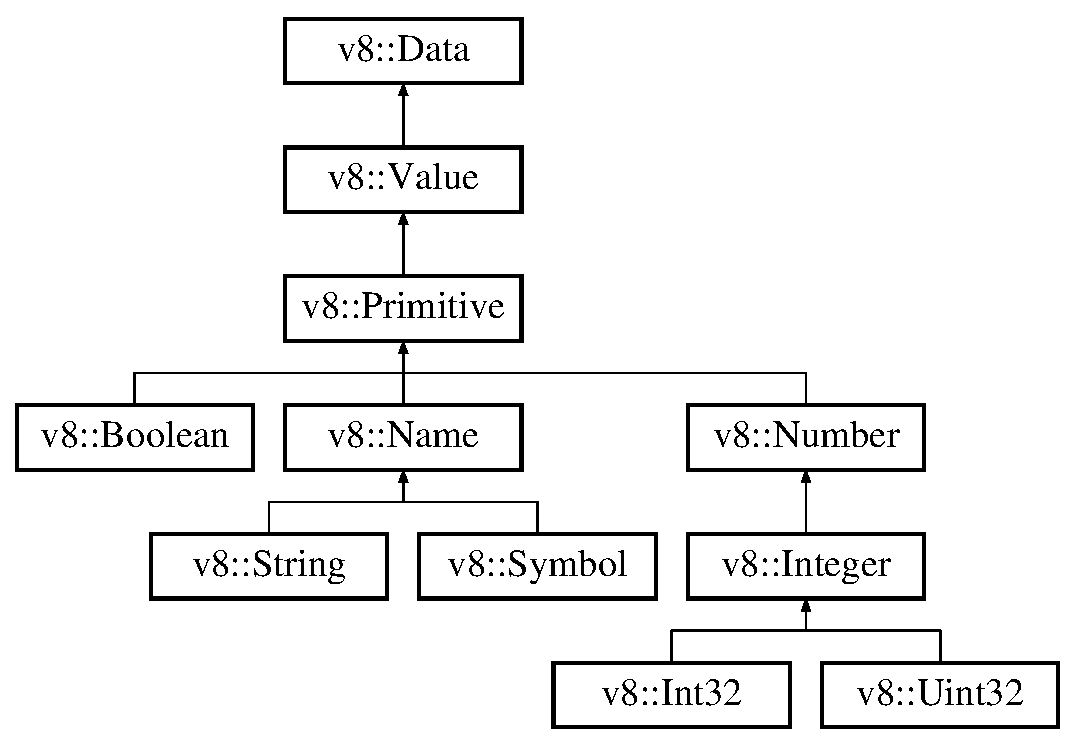
\includegraphics[height=6.000000cm]{classv8_1_1_primitive}
\end{center}
\end{figure}
\subsection*{Additional Inherited Members}


\subsection{Detailed Description}
The superclass of primitive values. See E\+C\+M\+A-\/262 4.\+3.\+2. 

The documentation for this class was generated from the following file\+:\begin{DoxyCompactItemize}
\item 
/\+Users/joshgav/node/v8/include/v8.\+h\end{DoxyCompactItemize}

\hypertarget{classv8_1_1_private}{}\section{v8\+:\+:Private Class Reference}
\label{classv8_1_1_private}\index{v8\+::\+Private@{v8\+::\+Private}}


{\ttfamily \#include $<$v8.\+h$>$}

Inheritance diagram for v8\+:\+:Private\+:\begin{figure}[H]
\begin{center}
\leavevmode
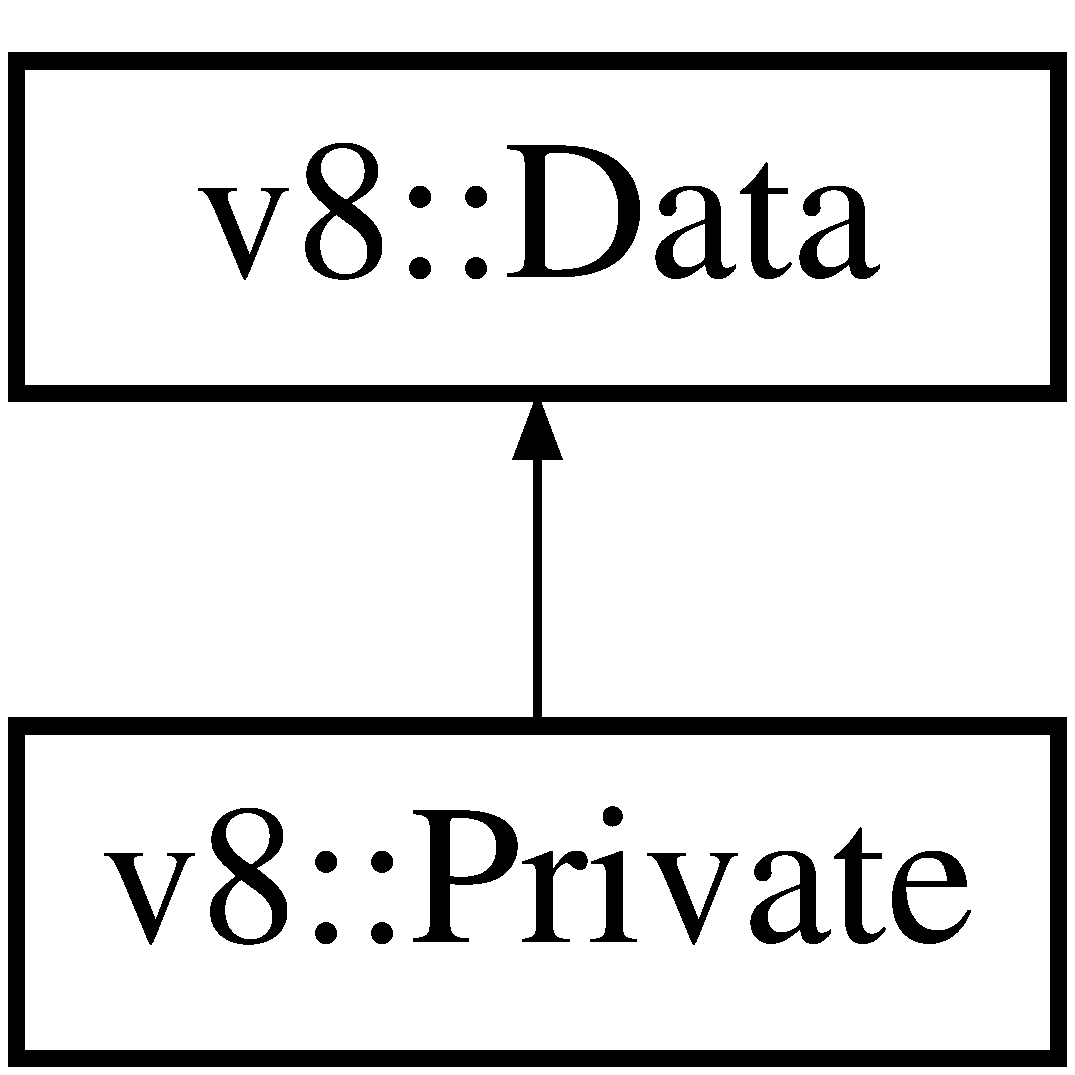
\includegraphics[height=2.000000cm]{classv8_1_1_private}
\end{center}
\end{figure}
\subsection*{Public Member Functions}
\begin{DoxyCompactItemize}
\item 
\hyperlink{classv8_1_1_local}{Local}$<$ \hyperlink{classv8_1_1_value}{Value} $>$ {\bfseries Name} () const \hypertarget{classv8_1_1_private_a346820b1e830262d7f4f31e5c5ac7304}{}\label{classv8_1_1_private_a346820b1e830262d7f4f31e5c5ac7304}

\end{DoxyCompactItemize}
\subsection*{Static Public Member Functions}
\begin{DoxyCompactItemize}
\item 
static \hyperlink{classv8_1_1_local}{Local}$<$ \hyperlink{classv8_1_1_private}{Private} $>$ {\bfseries New} (\hyperlink{classv8_1_1_isolate}{Isolate} $\ast$isolate, \hyperlink{classv8_1_1_local}{Local}$<$ \hyperlink{classv8_1_1_string}{String} $>$ name=\hyperlink{classv8_1_1_local}{Local}$<$ \hyperlink{classv8_1_1_string}{String} $>$())\hypertarget{classv8_1_1_private_ae43aa9516121ed7a24cf5bba1654b653}{}\label{classv8_1_1_private_ae43aa9516121ed7a24cf5bba1654b653}

\item 
static \hyperlink{classv8_1_1_local}{Local}$<$ \hyperlink{classv8_1_1_private}{Private} $>$ {\bfseries For\+Api} (\hyperlink{classv8_1_1_isolate}{Isolate} $\ast$isolate, \hyperlink{classv8_1_1_local}{Local}$<$ \hyperlink{classv8_1_1_string}{String} $>$ name)\hypertarget{classv8_1_1_private_a0ab8628387166b8a8abc6e9b6f40ad55}{}\label{classv8_1_1_private_a0ab8628387166b8a8abc6e9b6f40ad55}

\end{DoxyCompactItemize}


\subsection{Detailed Description}
A private symbol

This is an experimental feature. Use at your own risk. 

The documentation for this class was generated from the following file\+:\begin{DoxyCompactItemize}
\item 
include/v8.\+h\end{DoxyCompactItemize}

\hypertarget{classv8_1_1_promise}{}\section{v8\+:\+:Promise Class Reference}
\label{classv8_1_1_promise}\index{v8\+::\+Promise@{v8\+::\+Promise}}


{\ttfamily \#include $<$v8.\+h$>$}

Inheritance diagram for v8\+:\+:Promise\+:\begin{figure}[H]
\begin{center}
\leavevmode
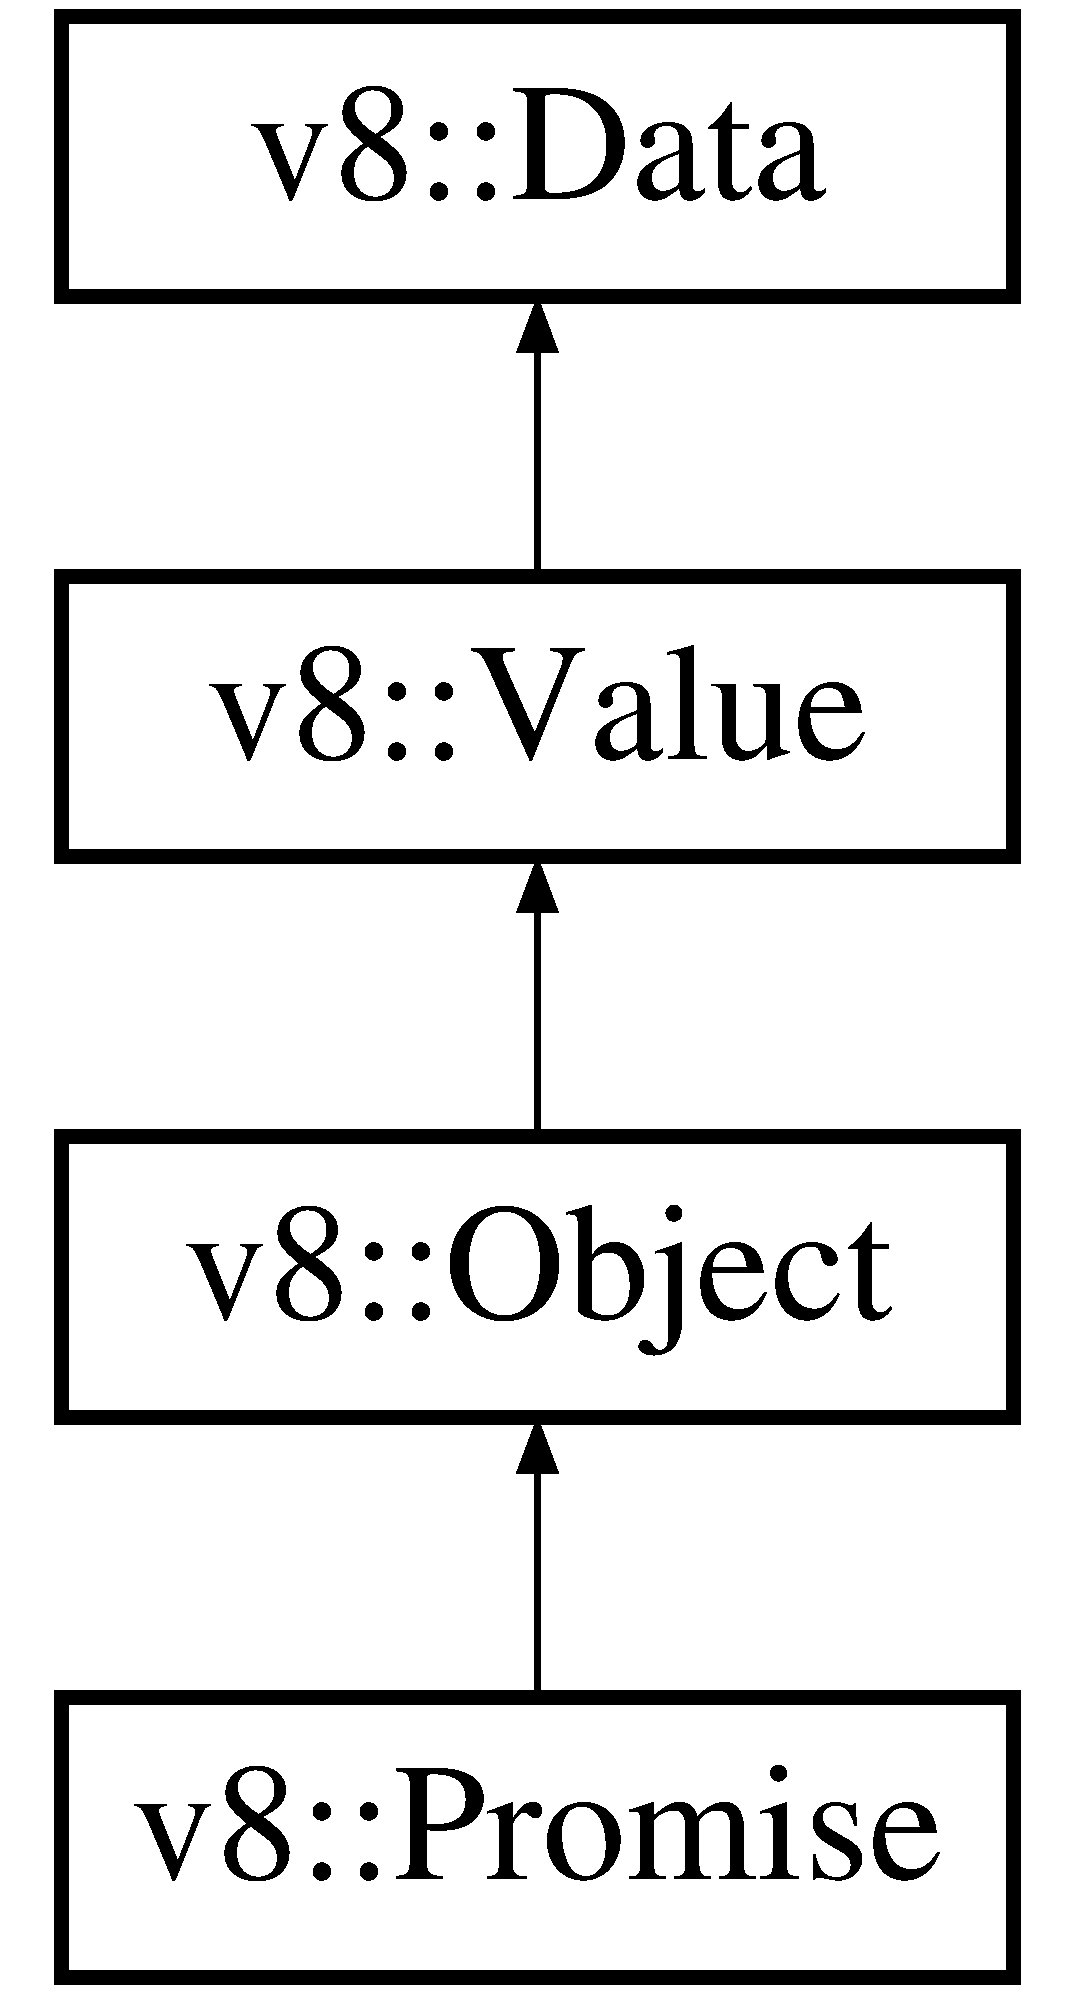
\includegraphics[height=4.000000cm]{classv8_1_1_promise}
\end{center}
\end{figure}
\subsection*{Classes}
\begin{DoxyCompactItemize}
\item 
class \hyperlink{classv8_1_1_promise_1_1_resolver}{Resolver}
\end{DoxyCompactItemize}
\subsection*{Public Member Functions}
\begin{DoxyCompactItemize}
\item 
\hyperlink{classv8_1_1_promise_a8378226f7b9e986184742dc5bb3cc78b}{V8\+\_\+\+D\+E\+P\+R\+E\+C\+A\+T\+ED} (\char`\"{}Use maybe version of Then\char`\"{}, Local$<$ \hyperlink{classv8_1_1_promise}{Promise} $>$ Chain(\hyperlink{classv8_1_1_local}{Local}$<$ \hyperlink{classv8_1_1_function}{Function} $>$ handler))
\item 
{\bfseries V8\+\_\+\+D\+E\+P\+R\+E\+C\+A\+T\+ED} (\char`\"{}Use Then\char`\"{}, V8\+\_\+\+W\+A\+R\+N\+\_\+\+U\+N\+U\+S\+E\+D\+\_\+\+R\+E\+S\+U\+LT \hyperlink{classv8_1_1_maybe_local}{Maybe\+Local}$<$ \hyperlink{classv8_1_1_promise}{Promise} $>$ Chain(                                                                       \hyperlink{classv8_1_1_local}{Local}$<$ \hyperlink{classv8_1_1_context}{Context} $>$ context, \hyperlink{classv8_1_1_local}{Local}$<$ \hyperlink{classv8_1_1_function}{Function} $>$ handler))\hypertarget{classv8_1_1_promise_a6a144ca5339ce1ccf856b4c142a9ff3e}{}\label{classv8_1_1_promise_a6a144ca5339ce1ccf856b4c142a9ff3e}

\item 
{\bfseries V8\+\_\+\+D\+E\+P\+R\+E\+C\+A\+T\+ED} (\char`\"{}Use maybe version\char`\"{}, Local$<$ \hyperlink{classv8_1_1_promise}{Promise} $>$ Catch(\hyperlink{classv8_1_1_local}{Local}$<$ \hyperlink{classv8_1_1_function}{Function} $>$ handler))\hypertarget{classv8_1_1_promise_abac3f6124a1393b13500f2579bd28513}{}\label{classv8_1_1_promise_abac3f6124a1393b13500f2579bd28513}

\item 
V8\+\_\+\+W\+A\+R\+N\+\_\+\+U\+N\+U\+S\+E\+D\+\_\+\+R\+E\+S\+U\+LT \hyperlink{classv8_1_1_maybe_local}{Maybe\+Local}$<$ \hyperlink{classv8_1_1_promise}{Promise} $>$ {\bfseries Catch} (\hyperlink{classv8_1_1_local}{Local}$<$ \hyperlink{classv8_1_1_context}{Context} $>$ context, \hyperlink{classv8_1_1_local}{Local}$<$ \hyperlink{classv8_1_1_function}{Function} $>$ handler)\hypertarget{classv8_1_1_promise_ab5b9bc0140b750cbf569f3a0e6c92b42}{}\label{classv8_1_1_promise_ab5b9bc0140b750cbf569f3a0e6c92b42}

\item 
{\bfseries V8\+\_\+\+D\+E\+P\+R\+E\+C\+A\+T\+ED} (\char`\"{}Use maybe version\char`\"{}, Local$<$ \hyperlink{classv8_1_1_promise}{Promise} $>$ Then(\hyperlink{classv8_1_1_local}{Local}$<$ \hyperlink{classv8_1_1_function}{Function} $>$ handler))\hypertarget{classv8_1_1_promise_a9bb6f0ee5815b09a9ad25b1f263a471c}{}\label{classv8_1_1_promise_a9bb6f0ee5815b09a9ad25b1f263a471c}

\item 
V8\+\_\+\+W\+A\+R\+N\+\_\+\+U\+N\+U\+S\+E\+D\+\_\+\+R\+E\+S\+U\+LT \hyperlink{classv8_1_1_maybe_local}{Maybe\+Local}$<$ \hyperlink{classv8_1_1_promise}{Promise} $>$ {\bfseries Then} (\hyperlink{classv8_1_1_local}{Local}$<$ \hyperlink{classv8_1_1_context}{Context} $>$ context, \hyperlink{classv8_1_1_local}{Local}$<$ \hyperlink{classv8_1_1_function}{Function} $>$ handler)\hypertarget{classv8_1_1_promise_af043d82818e1bbaf6c659e40bcf86c89}{}\label{classv8_1_1_promise_af043d82818e1bbaf6c659e40bcf86c89}

\item 
bool \hyperlink{classv8_1_1_promise_aeea8bdfdbe2291632d7f0d45394c1722}{Has\+Handler} ()
\end{DoxyCompactItemize}
\subsection*{Static Public Member Functions}
\begin{DoxyCompactItemize}
\item 
static V8\+\_\+\+I\+N\+L\+I\+NE \hyperlink{classv8_1_1_promise}{Promise} $\ast$ {\bfseries Cast} (\hyperlink{classv8_1_1_value}{Value} $\ast$obj)\hypertarget{classv8_1_1_promise_adfa3b953beb2678dd3b5d6ddb3f0746d}{}\label{classv8_1_1_promise_adfa3b953beb2678dd3b5d6ddb3f0746d}

\end{DoxyCompactItemize}
\subsection*{Static Private Member Functions}
\begin{DoxyCompactItemize}
\item 
static void {\bfseries Check\+Cast} (\hyperlink{classv8_1_1_value}{Value} $\ast$obj)\hypertarget{classv8_1_1_promise_a6c6f1b9b87d6fef2db0f16fb04bb6ed1}{}\label{classv8_1_1_promise_a6c6f1b9b87d6fef2db0f16fb04bb6ed1}

\end{DoxyCompactItemize}


\subsection{Detailed Description}
An instance of the built-\/in \hyperlink{classv8_1_1_promise}{Promise} constructor (E\+S6 draft). This A\+PI is experimental. Only works with --harmony flag. 

\subsection{Member Function Documentation}
\index{v8\+::\+Promise@{v8\+::\+Promise}!Has\+Handler@{Has\+Handler}}
\index{Has\+Handler@{Has\+Handler}!v8\+::\+Promise@{v8\+::\+Promise}}
\subsubsection[{\texorpdfstring{Has\+Handler()}{HasHandler()}}]{\setlength{\rightskip}{0pt plus 5cm}bool v8\+::\+Promise\+::\+Has\+Handler (
\begin{DoxyParamCaption}
{}
\end{DoxyParamCaption}
)}\hypertarget{classv8_1_1_promise_aeea8bdfdbe2291632d7f0d45394c1722}{}\label{classv8_1_1_promise_aeea8bdfdbe2291632d7f0d45394c1722}
Returns true if the promise has at least one derived promise, and therefore resolve/reject handlers (including default handler). \index{v8\+::\+Promise@{v8\+::\+Promise}!V8\+\_\+\+D\+E\+P\+R\+E\+C\+A\+T\+ED@{V8\+\_\+\+D\+E\+P\+R\+E\+C\+A\+T\+ED}}
\index{V8\+\_\+\+D\+E\+P\+R\+E\+C\+A\+T\+ED@{V8\+\_\+\+D\+E\+P\+R\+E\+C\+A\+T\+ED}!v8\+::\+Promise@{v8\+::\+Promise}}
\subsubsection[{\texorpdfstring{V8\+\_\+\+D\+E\+P\+R\+E\+C\+A\+T\+E\+D(""Use maybe version of Then"", Local$<$ Promise $>$ Chain(\+Local$<$ Function $>$ handler))}{V8_DEPRECATED("Use maybe version of Then", Local< Promise > Chain(Local< Function > handler))}}]{\setlength{\rightskip}{0pt plus 5cm}v8\+::\+Promise\+::\+V8\+\_\+\+D\+E\+P\+R\+E\+C\+A\+T\+ED (
\begin{DoxyParamCaption}
\item[{\char`\"{}Use maybe version of Then\char`\"{}}]{, }
\item[{{\bf Local}$<$ {\bf Promise} $>$ }]{ChainLocal$<$ Function $>$ handler}
\end{DoxyParamCaption}
)}\hypertarget{classv8_1_1_promise_a8378226f7b9e986184742dc5bb3cc78b}{}\label{classv8_1_1_promise_a8378226f7b9e986184742dc5bb3cc78b}
Register a resolution/rejection handler with a promise. The handler is given the respective resolution/rejection value as an argument. If the promise is already resolved/rejected, the handler is invoked at the end of turn. 

The documentation for this class was generated from the following file\+:\begin{DoxyCompactItemize}
\item 
/\+Users/joshgav/node/v8/include/v8.\+h\end{DoxyCompactItemize}

\hypertarget{classv8_1_1_promise_reject_message}{}\section{v8\+:\+:Promise\+Reject\+Message Class Reference}
\label{classv8_1_1_promise_reject_message}\index{v8\+::\+Promise\+Reject\+Message@{v8\+::\+Promise\+Reject\+Message}}
\subsection*{Public Member Functions}
\begin{DoxyCompactItemize}
\item 
{\bfseries Promise\+Reject\+Message} (\hyperlink{classv8_1_1_local}{Local}$<$ \hyperlink{classv8_1_1_promise}{Promise} $>$ promise, Promise\+Reject\+Event event, \hyperlink{classv8_1_1_local}{Local}$<$ \hyperlink{classv8_1_1_value}{Value} $>$ value, \hyperlink{classv8_1_1_local}{Local}$<$ \hyperlink{classv8_1_1_stack_trace}{Stack\+Trace} $>$ stack\+\_\+trace)\hypertarget{classv8_1_1_promise_reject_message_a052df173c75f1eb31b252714c88f3362}{}\label{classv8_1_1_promise_reject_message_a052df173c75f1eb31b252714c88f3362}

\item 
V8\+\_\+\+I\+N\+L\+I\+NE \hyperlink{classv8_1_1_local}{Local}$<$ \hyperlink{classv8_1_1_promise}{Promise} $>$ {\bfseries Get\+Promise} () const \hypertarget{classv8_1_1_promise_reject_message_a8582107385b66f911c6d4c9a17890222}{}\label{classv8_1_1_promise_reject_message_a8582107385b66f911c6d4c9a17890222}

\item 
V8\+\_\+\+I\+N\+L\+I\+NE Promise\+Reject\+Event {\bfseries Get\+Event} () const \hypertarget{classv8_1_1_promise_reject_message_a1380024500dac27eb74665701a80c6b0}{}\label{classv8_1_1_promise_reject_message_a1380024500dac27eb74665701a80c6b0}

\item 
V8\+\_\+\+I\+N\+L\+I\+NE \hyperlink{classv8_1_1_local}{Local}$<$ \hyperlink{classv8_1_1_value}{Value} $>$ {\bfseries Get\+Value} () const \hypertarget{classv8_1_1_promise_reject_message_ad87ec78d2e817b623d996f8db7d45ffc}{}\label{classv8_1_1_promise_reject_message_ad87ec78d2e817b623d996f8db7d45ffc}

\item 
{\bfseries V8\+\_\+\+D\+E\+P\+R\+E\+C\+A\+T\+ED} (\char`\"{}Use \hyperlink{classv8_1_1_exception_a8d575a721cf0fd5b325afb8b586c0d1e}{v8\+::\+Exception\+::\+Create\+Message}(Get\+Value())-\/$>$Get\+Stack\+Trace()\char`\"{}, V8\+\_\+\+I\+N\+L\+I\+NE \hyperlink{classv8_1_1_local}{Local}$<$ \hyperlink{classv8_1_1_stack_trace}{Stack\+Trace} $>$ Get\+Stack\+Trace() const)\hypertarget{classv8_1_1_promise_reject_message_af768aa21023875a4037d797d1e91fe42}{}\label{classv8_1_1_promise_reject_message_af768aa21023875a4037d797d1e91fe42}

\end{DoxyCompactItemize}
\subsection*{Private Attributes}
\begin{DoxyCompactItemize}
\item 
\hyperlink{classv8_1_1_local}{Local}$<$ \hyperlink{classv8_1_1_promise}{Promise} $>$ {\bfseries promise\+\_\+}\hypertarget{classv8_1_1_promise_reject_message_a21a47d63f57740ac79e90a1f8d4de1a3}{}\label{classv8_1_1_promise_reject_message_a21a47d63f57740ac79e90a1f8d4de1a3}

\item 
Promise\+Reject\+Event {\bfseries event\+\_\+}\hypertarget{classv8_1_1_promise_reject_message_a40c18262bff9955b6accec1a6c069a58}{}\label{classv8_1_1_promise_reject_message_a40c18262bff9955b6accec1a6c069a58}

\item 
\hyperlink{classv8_1_1_local}{Local}$<$ \hyperlink{classv8_1_1_value}{Value} $>$ {\bfseries value\+\_\+}\hypertarget{classv8_1_1_promise_reject_message_a06067111ef1233d7c3b38fcc8a77d5a2}{}\label{classv8_1_1_promise_reject_message_a06067111ef1233d7c3b38fcc8a77d5a2}

\item 
\hyperlink{classv8_1_1_local}{Local}$<$ \hyperlink{classv8_1_1_stack_trace}{Stack\+Trace} $>$ {\bfseries stack\+\_\+trace\+\_\+}\hypertarget{classv8_1_1_promise_reject_message_a28e8114e1e9d7b9ed60a546a3fcf7ff7}{}\label{classv8_1_1_promise_reject_message_a28e8114e1e9d7b9ed60a546a3fcf7ff7}

\end{DoxyCompactItemize}


The documentation for this class was generated from the following file\+:\begin{DoxyCompactItemize}
\item 
include/v8.\+h\end{DoxyCompactItemize}

\hypertarget{classv8_1_1_property_callback_info}{}\section{v8\+:\+:Property\+Callback\+Info$<$ T $>$ Class Template Reference}
\label{classv8_1_1_property_callback_info}\index{v8\+::\+Property\+Callback\+Info$<$ T $>$@{v8\+::\+Property\+Callback\+Info$<$ T $>$}}


{\ttfamily \#include $<$v8.\+h$>$}

\subsection*{Public Member Functions}
\begin{DoxyCompactItemize}
\item 
V8\+\_\+\+I\+N\+L\+I\+NE \hyperlink{classv8_1_1_isolate}{Isolate} $\ast$ {\bfseries Get\+Isolate} () const \hypertarget{classv8_1_1_property_callback_info_a066d0c9eee98f80fb78d97961eafa8ad}{}\label{classv8_1_1_property_callback_info_a066d0c9eee98f80fb78d97961eafa8ad}

\item 
V8\+\_\+\+I\+N\+L\+I\+NE \hyperlink{classv8_1_1_local}{Local}$<$ \hyperlink{classv8_1_1_value}{Value} $>$ {\bfseries Data} () const \hypertarget{classv8_1_1_property_callback_info_a64edbaeb902e360fc2a4d353c8c4930f}{}\label{classv8_1_1_property_callback_info_a64edbaeb902e360fc2a4d353c8c4930f}

\item 
V8\+\_\+\+I\+N\+L\+I\+NE \hyperlink{classv8_1_1_local}{Local}$<$ \hyperlink{classv8_1_1_object}{Object} $>$ {\bfseries This} () const \hypertarget{classv8_1_1_property_callback_info_a747202a7d4db0b930f19f9466c3a5acb}{}\label{classv8_1_1_property_callback_info_a747202a7d4db0b930f19f9466c3a5acb}

\item 
V8\+\_\+\+I\+N\+L\+I\+NE \hyperlink{classv8_1_1_local}{Local}$<$ \hyperlink{classv8_1_1_object}{Object} $>$ {\bfseries Holder} () const \hypertarget{classv8_1_1_property_callback_info_a8eb97205ce7bd25b446b03643d02570d}{}\label{classv8_1_1_property_callback_info_a8eb97205ce7bd25b446b03643d02570d}

\item 
V8\+\_\+\+I\+N\+L\+I\+NE \hyperlink{classv8_1_1_return_value}{Return\+Value}$<$ T $>$ {\bfseries Get\+Return\+Value} () const \hypertarget{classv8_1_1_property_callback_info_a4e9bc4da66ed3ea21aac7dbb9c11465b}{}\label{classv8_1_1_property_callback_info_a4e9bc4da66ed3ea21aac7dbb9c11465b}

\item 
V8\+\_\+\+I\+N\+L\+I\+NE bool {\bfseries Should\+Throw\+On\+Error} () const \hypertarget{classv8_1_1_property_callback_info_a6b5104e088ca57f80be66435d6b2f0e2}{}\label{classv8_1_1_property_callback_info_a6b5104e088ca57f80be66435d6b2f0e2}

\end{DoxyCompactItemize}
\subsection*{Static Public Attributes}
\begin{DoxyCompactItemize}
\item 
static const int {\bfseries k\+Args\+Length} = 7\hypertarget{classv8_1_1_property_callback_info_a9fc9663a2e23f9324fe61f92d1e7e5b5}{}\label{classv8_1_1_property_callback_info_a9fc9663a2e23f9324fe61f92d1e7e5b5}

\end{DoxyCompactItemize}
\subsection*{Protected Member Functions}
\begin{DoxyCompactItemize}
\item 
V8\+\_\+\+I\+N\+L\+I\+NE {\bfseries Property\+Callback\+Info} (internal\+::\+Object $\ast$$\ast$args)\hypertarget{classv8_1_1_property_callback_info_aa666043c86d4db9a57a3ac866c78ee0e}{}\label{classv8_1_1_property_callback_info_aa666043c86d4db9a57a3ac866c78ee0e}

\end{DoxyCompactItemize}
\subsection*{Protected Attributes}
\begin{DoxyCompactItemize}
\item 
internal\+::\+Object $\ast$$\ast$ {\bfseries args\+\_\+}\hypertarget{classv8_1_1_property_callback_info_a57b2243627071c62ed3900a741a41a0b}{}\label{classv8_1_1_property_callback_info_a57b2243627071c62ed3900a741a41a0b}

\end{DoxyCompactItemize}
\subsection*{Static Protected Attributes}
\begin{DoxyCompactItemize}
\item 
static const int {\bfseries k\+Should\+Throw\+On\+Error\+Index} = 0\hypertarget{classv8_1_1_property_callback_info_aab5f05fed930b0cad97ed7f96520f60e}{}\label{classv8_1_1_property_callback_info_aab5f05fed930b0cad97ed7f96520f60e}

\item 
static const int {\bfseries k\+Holder\+Index} = 1\hypertarget{classv8_1_1_property_callback_info_a8598985473483dfadba4e4c67251675b}{}\label{classv8_1_1_property_callback_info_a8598985473483dfadba4e4c67251675b}

\item 
static const int {\bfseries k\+Isolate\+Index} = 2\hypertarget{classv8_1_1_property_callback_info_a59ba899cb580bc5e8adca6f799db3e2a}{}\label{classv8_1_1_property_callback_info_a59ba899cb580bc5e8adca6f799db3e2a}

\item 
static const int {\bfseries k\+Return\+Value\+Default\+Value\+Index} = 3\hypertarget{classv8_1_1_property_callback_info_a00849f770023891d1466176f5e0c8539}{}\label{classv8_1_1_property_callback_info_a00849f770023891d1466176f5e0c8539}

\item 
static const int {\bfseries k\+Return\+Value\+Index} = 4\hypertarget{classv8_1_1_property_callback_info_ae16cdf2c6ce787b21d94953cd514ed0e}{}\label{classv8_1_1_property_callback_info_ae16cdf2c6ce787b21d94953cd514ed0e}

\item 
static const int {\bfseries k\+Data\+Index} = 5\hypertarget{classv8_1_1_property_callback_info_a39fc5d6aaccb2916af503c7120ab99c5}{}\label{classv8_1_1_property_callback_info_a39fc5d6aaccb2916af503c7120ab99c5}

\item 
static const int {\bfseries k\+This\+Index} = 6\hypertarget{classv8_1_1_property_callback_info_a715d28b9c57a581de1698673c9b9eb8a}{}\label{classv8_1_1_property_callback_info_a715d28b9c57a581de1698673c9b9eb8a}

\end{DoxyCompactItemize}
\subsection*{Friends}
\begin{DoxyCompactItemize}
\item 
class {\bfseries Macro\+Assembler}\hypertarget{classv8_1_1_property_callback_info_ae605ff1d9d93250ace8a0a8b8d1dee67}{}\label{classv8_1_1_property_callback_info_ae605ff1d9d93250ace8a0a8b8d1dee67}

\item 
class {\bfseries internal\+::\+Property\+Callback\+Arguments}\hypertarget{classv8_1_1_property_callback_info_a1ba96a1268a72c23f50314cd99c76f1b}{}\label{classv8_1_1_property_callback_info_a1ba96a1268a72c23f50314cd99c76f1b}

\item 
class {\bfseries internal\+::\+Custom\+Arguments$<$ Property\+Callback\+Info $>$}\hypertarget{classv8_1_1_property_callback_info_ad1d1e15ddaed2ab44e8f21c5564881ba}{}\label{classv8_1_1_property_callback_info_ad1d1e15ddaed2ab44e8f21c5564881ba}

\end{DoxyCompactItemize}


\subsection{Detailed Description}
\subsubsection*{template$<$typename T$>$\\*
class v8\+::\+Property\+Callback\+Info$<$ T $>$}

The information passed to a property callback about the context of the property access. 

The documentation for this class was generated from the following file\+:\begin{DoxyCompactItemize}
\item 
include/v8.\+h\end{DoxyCompactItemize}

\hypertarget{classv8_1_1_proxy}{}\section{v8\+:\+:Proxy Class Reference}
\label{classv8_1_1_proxy}\index{v8\+::\+Proxy@{v8\+::\+Proxy}}


{\ttfamily \#include $<$v8.\+h$>$}

Inheritance diagram for v8\+:\+:Proxy\+:\begin{figure}[H]
\begin{center}
\leavevmode
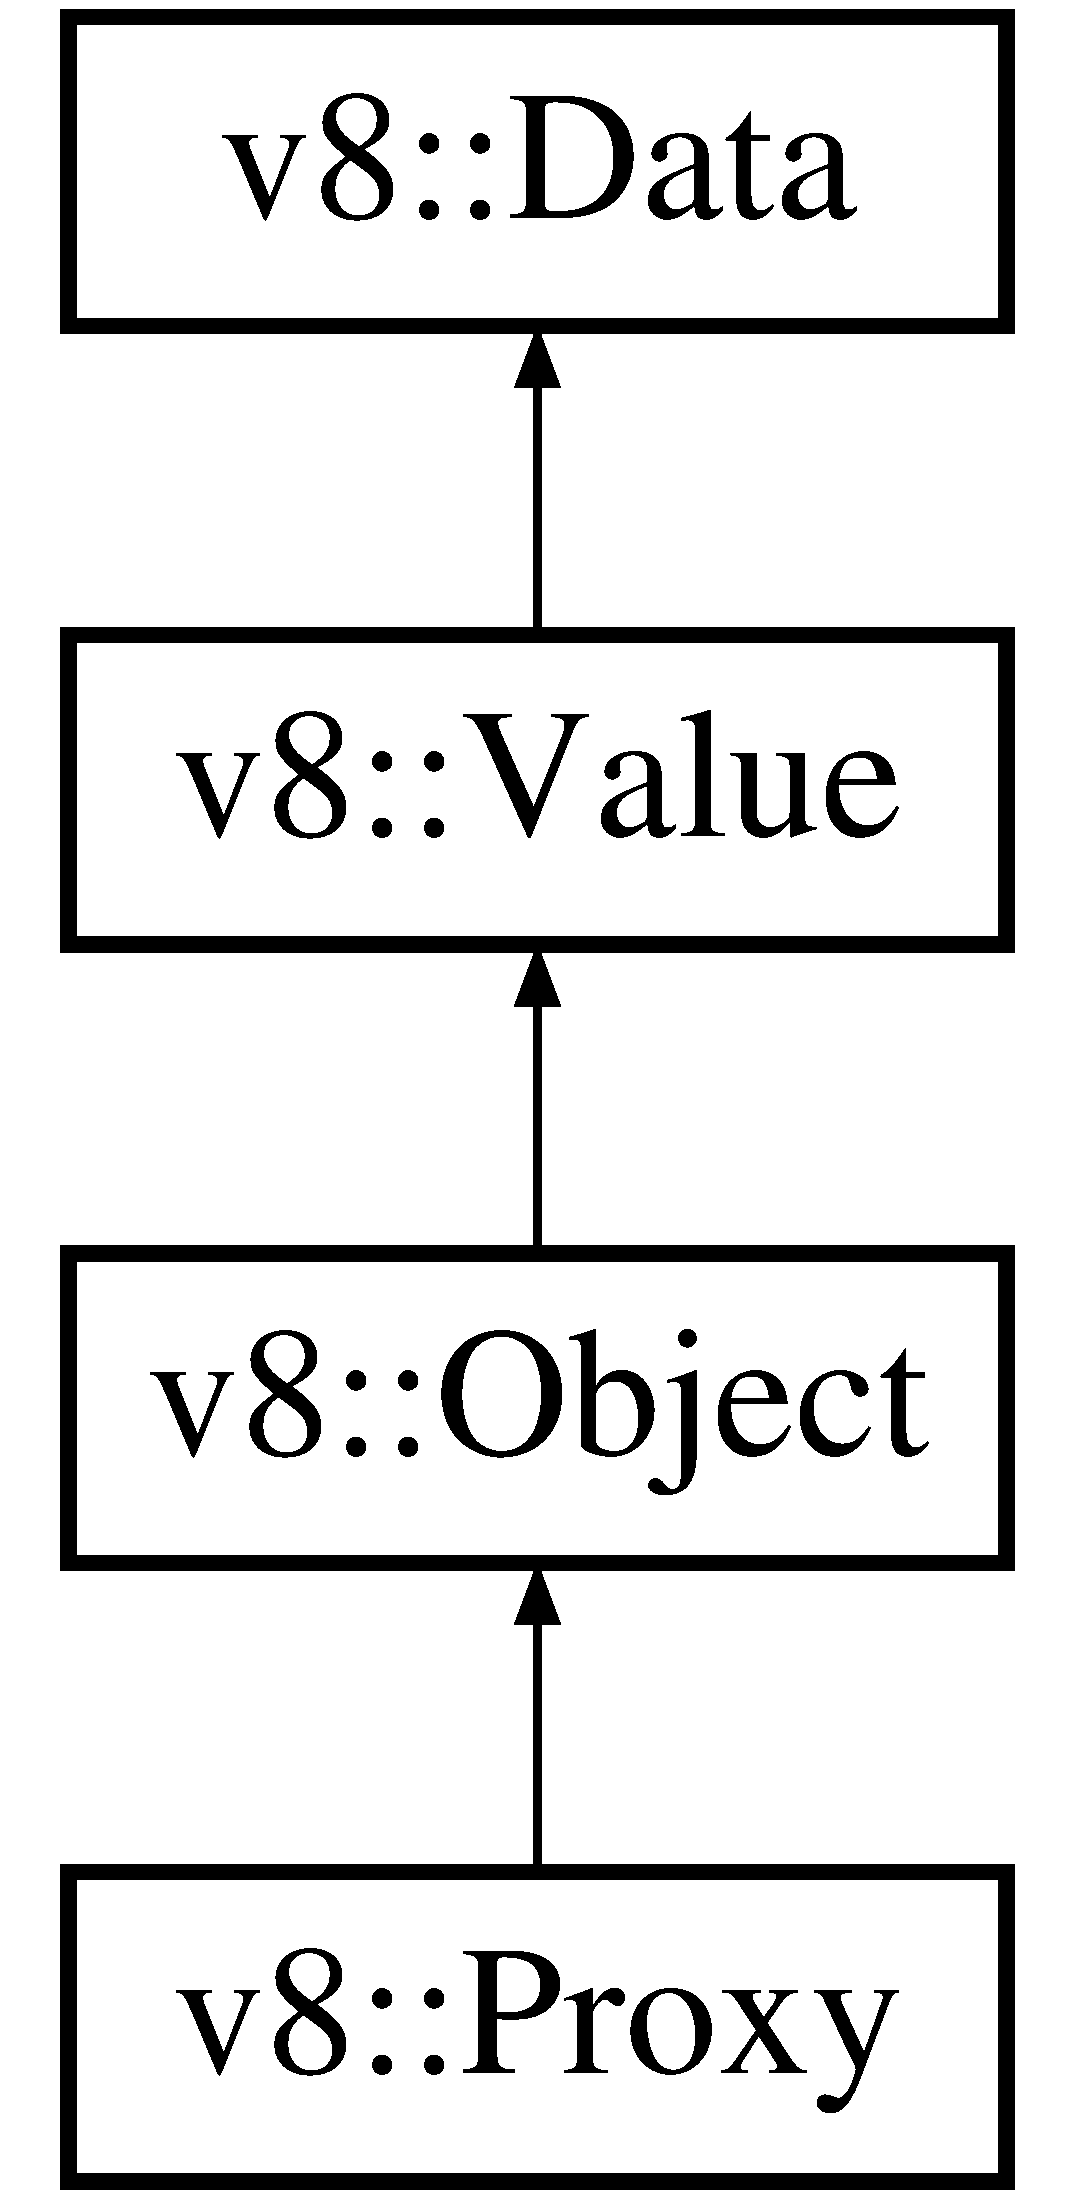
\includegraphics[height=4.000000cm]{classv8_1_1_proxy}
\end{center}
\end{figure}
\subsection*{Public Member Functions}
\begin{DoxyCompactItemize}
\item 
\hyperlink{classv8_1_1_local}{Local}$<$ \hyperlink{classv8_1_1_object}{Object} $>$ {\bfseries Get\+Target} ()\hypertarget{classv8_1_1_proxy_acfe2ad3df620f6418239c6be170c04db}{}\label{classv8_1_1_proxy_acfe2ad3df620f6418239c6be170c04db}

\item 
\hyperlink{classv8_1_1_local}{Local}$<$ \hyperlink{classv8_1_1_value}{Value} $>$ {\bfseries Get\+Handler} ()\hypertarget{classv8_1_1_proxy_a5343ef97e20c0e61996d194e1a48e0e4}{}\label{classv8_1_1_proxy_a5343ef97e20c0e61996d194e1a48e0e4}

\item 
bool {\bfseries Is\+Revoked} ()\hypertarget{classv8_1_1_proxy_ad6100ff322bd5b0297deea20237ff065}{}\label{classv8_1_1_proxy_ad6100ff322bd5b0297deea20237ff065}

\item 
void {\bfseries Revoke} ()\hypertarget{classv8_1_1_proxy_a24a05c4dc89a74406456df8c14adff7e}{}\label{classv8_1_1_proxy_a24a05c4dc89a74406456df8c14adff7e}

\end{DoxyCompactItemize}
\subsection*{Static Public Member Functions}
\begin{DoxyCompactItemize}
\item 
static \hyperlink{classv8_1_1_maybe_local}{Maybe\+Local}$<$ \hyperlink{classv8_1_1_proxy}{Proxy} $>$ \hyperlink{classv8_1_1_proxy_a08984acd4a8a94f125afd76b317f66ea}{New} (\hyperlink{classv8_1_1_local}{Local}$<$ \hyperlink{classv8_1_1_context}{Context} $>$ context, \hyperlink{classv8_1_1_local}{Local}$<$ \hyperlink{classv8_1_1_object}{Object} $>$ local\+\_\+target, \hyperlink{classv8_1_1_local}{Local}$<$ \hyperlink{classv8_1_1_object}{Object} $>$ local\+\_\+handler)
\item 
static V8\+\_\+\+I\+N\+L\+I\+NE \hyperlink{classv8_1_1_proxy}{Proxy} $\ast$ {\bfseries Cast} (\hyperlink{classv8_1_1_value}{Value} $\ast$obj)\hypertarget{classv8_1_1_proxy_a6562478fdedab6fa0fe20ede066b2a78}{}\label{classv8_1_1_proxy_a6562478fdedab6fa0fe20ede066b2a78}

\end{DoxyCompactItemize}
\subsection*{Static Private Member Functions}
\begin{DoxyCompactItemize}
\item 
static void {\bfseries Check\+Cast} (\hyperlink{classv8_1_1_value}{Value} $\ast$obj)\hypertarget{classv8_1_1_proxy_a4b644259b25d57fed195e45887068cac}{}\label{classv8_1_1_proxy_a4b644259b25d57fed195e45887068cac}

\end{DoxyCompactItemize}


\subsection{Detailed Description}
An instance of the built-\/in \hyperlink{classv8_1_1_proxy}{Proxy} constructor (E\+C\+M\+A-\/262, 6th Edition, 26.\+2.\+1). 

\subsection{Member Function Documentation}
\index{v8\+::\+Proxy@{v8\+::\+Proxy}!New@{New}}
\index{New@{New}!v8\+::\+Proxy@{v8\+::\+Proxy}}
\subsubsection[{\texorpdfstring{New(\+Local$<$ Context $>$ context, Local$<$ Object $>$ local\+\_\+target, Local$<$ Object $>$ local\+\_\+handler)}{New(Local< Context > context, Local< Object > local_target, Local< Object > local_handler)}}]{\setlength{\rightskip}{0pt plus 5cm}{\bf Maybe\+Local}$<$ {\bf Proxy} $>$ v8\+::\+Proxy\+::\+New (
\begin{DoxyParamCaption}
\item[{{\bf Local}$<$ {\bf Context} $>$}]{context, }
\item[{{\bf Local}$<$ {\bf Object} $>$}]{local\+\_\+target, }
\item[{{\bf Local}$<$ {\bf Object} $>$}]{local\+\_\+handler}
\end{DoxyParamCaption}
)\hspace{0.3cm}{\ttfamily [static]}}\hypertarget{classv8_1_1_proxy_a08984acd4a8a94f125afd76b317f66ea}{}\label{classv8_1_1_proxy_a08984acd4a8a94f125afd76b317f66ea}
Creates a new empty \hyperlink{classv8_1_1_map}{Map}. 

The documentation for this class was generated from the following files\+:\begin{DoxyCompactItemize}
\item 
/\+Users/joshgav/node/v8/include/v8.\+h\item 
/\+Users/joshgav/node/v8/src/api.\+cc\end{DoxyCompactItemize}

\hypertarget{classv8_1_1_reg_exp}{}\section{v8\+:\+:Reg\+Exp Class Reference}
\label{classv8_1_1_reg_exp}\index{v8\+::\+Reg\+Exp@{v8\+::\+Reg\+Exp}}


{\ttfamily \#include $<$v8.\+h$>$}

Inheritance diagram for v8\+:\+:Reg\+Exp\+:\begin{figure}[H]
\begin{center}
\leavevmode
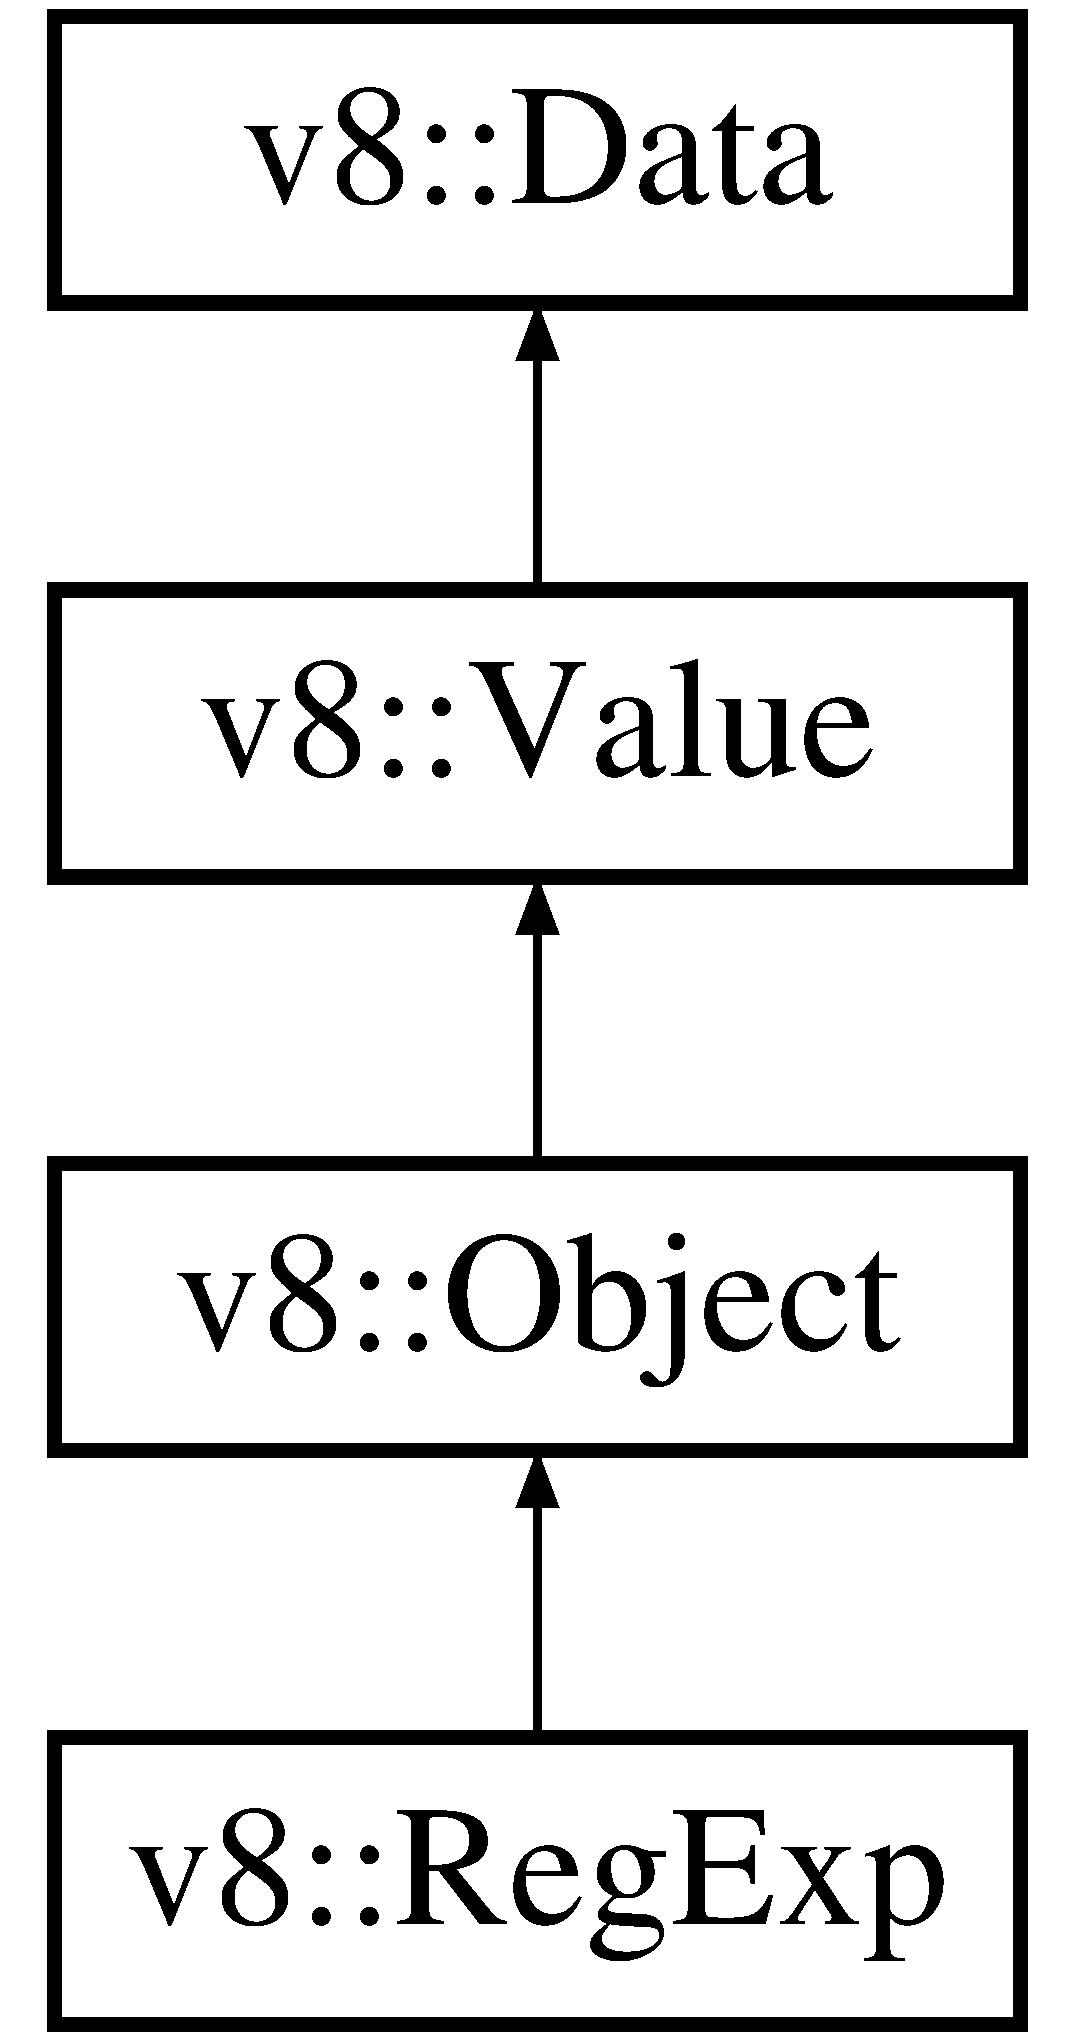
\includegraphics[height=4.000000cm]{classv8_1_1_reg_exp}
\end{center}
\end{figure}
\subsection*{Public Types}
\begin{DoxyCompactItemize}
\item 
enum \hyperlink{classv8_1_1_reg_exp_aa4718a5c1f18472aff3bf51ed694fc5a}{Flags} \{ \\*
{\bfseries k\+None} = 0, 
\\*
{\bfseries k\+Global} = 1, 
\\*
{\bfseries k\+Ignore\+Case} = 2, 
\\*
{\bfseries k\+Multiline} = 4, 
\\*
{\bfseries k\+Sticky} = 8, 
\\*
{\bfseries k\+Unicode} = 16
 \}
\end{DoxyCompactItemize}
\subsection*{Public Member Functions}
\begin{DoxyCompactItemize}
\item 
\hyperlink{classv8_1_1_local}{Local}$<$ \hyperlink{classv8_1_1_string}{String} $>$ \hyperlink{classv8_1_1_reg_exp_a448213f2a92d964ed260b51429d5e590}{Get\+Source} () const 
\item 
\hyperlink{classv8_1_1_reg_exp_aa4718a5c1f18472aff3bf51ed694fc5a}{Flags} \hyperlink{classv8_1_1_reg_exp_ad5a5e77e6e626b3c7c69eef7ba2908cc}{Get\+Flags} () const 
\end{DoxyCompactItemize}
\subsection*{Static Public Member Functions}
\begin{DoxyCompactItemize}
\item 
static \hyperlink{classv8_1_1_reg_exp_a9793a5a1e31b5ea0563d96d8c74c01ff}{V8\+\_\+\+D\+E\+P\+R\+E\+C\+A\+T\+E\+\_\+\+S\+O\+ON} (\char`\"{}Use maybe version\char`\"{}, Local$<$ \hyperlink{classv8_1_1_reg_exp}{Reg\+Exp} $>$ New(\hyperlink{classv8_1_1_local}{Local}$<$ \hyperlink{classv8_1_1_string}{String} $>$ pattern,                                                                                                                                                                           \hyperlink{classv8_1_1_reg_exp_aa4718a5c1f18472aff3bf51ed694fc5a}{Flags} flags))
\item 
static V8\+\_\+\+W\+A\+R\+N\+\_\+\+U\+N\+U\+S\+E\+D\+\_\+\+R\+E\+S\+U\+LT \hyperlink{classv8_1_1_maybe_local}{Maybe\+Local}$<$ \hyperlink{classv8_1_1_reg_exp}{Reg\+Exp} $>$ {\bfseries New} (\hyperlink{classv8_1_1_local}{Local}$<$ \hyperlink{classv8_1_1_context}{Context} $>$ context, \hyperlink{classv8_1_1_local}{Local}$<$ \hyperlink{classv8_1_1_string}{String} $>$ pattern, \hyperlink{classv8_1_1_reg_exp_aa4718a5c1f18472aff3bf51ed694fc5a}{Flags} flags)\hypertarget{classv8_1_1_reg_exp_a805f632fe98d58160773a4ba1e424b15}{}\label{classv8_1_1_reg_exp_a805f632fe98d58160773a4ba1e424b15}

\item 
static V8\+\_\+\+I\+N\+L\+I\+NE \hyperlink{classv8_1_1_reg_exp}{Reg\+Exp} $\ast$ {\bfseries Cast} (\hyperlink{classv8_1_1_value}{v8\+::\+Value} $\ast$obj)\hypertarget{classv8_1_1_reg_exp_ac06d8f61c0ebb2e7292e6aeff7108f26}{}\label{classv8_1_1_reg_exp_ac06d8f61c0ebb2e7292e6aeff7108f26}

\end{DoxyCompactItemize}
\subsection*{Static Private Member Functions}
\begin{DoxyCompactItemize}
\item 
static void {\bfseries Check\+Cast} (\hyperlink{classv8_1_1_value}{v8\+::\+Value} $\ast$obj)\hypertarget{classv8_1_1_reg_exp_a6d6d2c215db79f12f9d9016b9f725522}{}\label{classv8_1_1_reg_exp_a6d6d2c215db79f12f9d9016b9f725522}

\end{DoxyCompactItemize}


\subsection{Detailed Description}
An instance of the built-\/in \hyperlink{classv8_1_1_reg_exp}{Reg\+Exp} constructor (E\+C\+M\+A-\/262, 15.\+10). 

\subsection{Member Enumeration Documentation}
\index{v8\+::\+Reg\+Exp@{v8\+::\+Reg\+Exp}!Flags@{Flags}}
\index{Flags@{Flags}!v8\+::\+Reg\+Exp@{v8\+::\+Reg\+Exp}}
\subsubsection[{\texorpdfstring{Flags}{Flags}}]{\setlength{\rightskip}{0pt plus 5cm}enum {\bf v8\+::\+Reg\+Exp\+::\+Flags}}\hypertarget{classv8_1_1_reg_exp_aa4718a5c1f18472aff3bf51ed694fc5a}{}\label{classv8_1_1_reg_exp_aa4718a5c1f18472aff3bf51ed694fc5a}
Regular expression flag bits. They can be or\textquotesingle{}ed to enable a set of flags. 

\subsection{Member Function Documentation}
\index{v8\+::\+Reg\+Exp@{v8\+::\+Reg\+Exp}!Get\+Flags@{Get\+Flags}}
\index{Get\+Flags@{Get\+Flags}!v8\+::\+Reg\+Exp@{v8\+::\+Reg\+Exp}}
\subsubsection[{\texorpdfstring{Get\+Flags() const }{GetFlags() const }}]{\setlength{\rightskip}{0pt plus 5cm}{\bf Flags} v8\+::\+Reg\+Exp\+::\+Get\+Flags (
\begin{DoxyParamCaption}
{}
\end{DoxyParamCaption}
) const}\hypertarget{classv8_1_1_reg_exp_ad5a5e77e6e626b3c7c69eef7ba2908cc}{}\label{classv8_1_1_reg_exp_ad5a5e77e6e626b3c7c69eef7ba2908cc}
Returns the flags bit field. \index{v8\+::\+Reg\+Exp@{v8\+::\+Reg\+Exp}!Get\+Source@{Get\+Source}}
\index{Get\+Source@{Get\+Source}!v8\+::\+Reg\+Exp@{v8\+::\+Reg\+Exp}}
\subsubsection[{\texorpdfstring{Get\+Source() const }{GetSource() const }}]{\setlength{\rightskip}{0pt plus 5cm}{\bf Local}$<${\bf String}$>$ v8\+::\+Reg\+Exp\+::\+Get\+Source (
\begin{DoxyParamCaption}
{}
\end{DoxyParamCaption}
) const}\hypertarget{classv8_1_1_reg_exp_a448213f2a92d964ed260b51429d5e590}{}\label{classv8_1_1_reg_exp_a448213f2a92d964ed260b51429d5e590}
Returns the value of the source property\+: a string representing the regular expression. \index{v8\+::\+Reg\+Exp@{v8\+::\+Reg\+Exp}!V8\+\_\+\+D\+E\+P\+R\+E\+C\+A\+T\+E\+\_\+\+S\+O\+ON@{V8\+\_\+\+D\+E\+P\+R\+E\+C\+A\+T\+E\+\_\+\+S\+O\+ON}}
\index{V8\+\_\+\+D\+E\+P\+R\+E\+C\+A\+T\+E\+\_\+\+S\+O\+ON@{V8\+\_\+\+D\+E\+P\+R\+E\+C\+A\+T\+E\+\_\+\+S\+O\+ON}!v8\+::\+Reg\+Exp@{v8\+::\+Reg\+Exp}}
\subsubsection[{\texorpdfstring{V8\+\_\+\+D\+E\+P\+R\+E\+C\+A\+T\+E\+\_\+\+S\+O\+O\+N(""Use maybe version"", Local$<$ Reg\+Exp $>$ New(\+Local$<$ String $>$ pattern,                                                                                                                                                                           Flags flags))}{V8_DEPRECATE_SOON("Use maybe version", Local< RegExp > New(Local< String > pattern,                                                                                                                                                                           Flags flags))}}]{\setlength{\rightskip}{0pt plus 5cm}static v8\+::\+Reg\+Exp\+::\+V8\+\_\+\+D\+E\+P\+R\+E\+C\+A\+T\+E\+\_\+\+S\+O\+ON (
\begin{DoxyParamCaption}
\item[{\char`\"{}Use maybe version\char`\"{}}]{, }
\item[{{\bf Local}$<$ {\bf Reg\+Exp} $>$ }]{NewLocal$<$ String $>$ pattern,                                                                                                                                                                                                                                                                                                                                                   Flags flags}
\end{DoxyParamCaption}
)\hspace{0.3cm}{\ttfamily [static]}}\hypertarget{classv8_1_1_reg_exp_a9793a5a1e31b5ea0563d96d8c74c01ff}{}\label{classv8_1_1_reg_exp_a9793a5a1e31b5ea0563d96d8c74c01ff}
Creates a regular expression from the given pattern string and the flags bit field. May throw a Java\+Script exception as described in E\+C\+M\+A-\/262, 15.\+10.\+4.\+1.

For example, Reg\+Exp\+::\+New(v8\+::\+String\+::\+New(\char`\"{}foo\char`\"{}), static\+\_\+cast$<$\+Reg\+Exp\+::\+Flags$>$(k\+Global $\vert$ k\+Multiline)) is equivalent to evaluating \char`\"{}/foo/gm\char`\"{}. 

The documentation for this class was generated from the following file\+:\begin{DoxyCompactItemize}
\item 
include/v8.\+h\end{DoxyCompactItemize}

\hypertarget{structv8_1_1_register_state}{}\section{v8\+:\+:Register\+State Struct Reference}
\label{structv8_1_1_register_state}\index{v8\+::\+Register\+State@{v8\+::\+Register\+State}}
\subsection*{Public Attributes}
\begin{DoxyCompactItemize}
\item 
void $\ast$ {\bfseries pc}\hypertarget{structv8_1_1_register_state_aa0d0327871d9f95d5e64f47b7f183907}{}\label{structv8_1_1_register_state_aa0d0327871d9f95d5e64f47b7f183907}

\item 
void $\ast$ {\bfseries sp}\hypertarget{structv8_1_1_register_state_a867bb9d0b9e81c3f7256aa81dc0daee4}{}\label{structv8_1_1_register_state_a867bb9d0b9e81c3f7256aa81dc0daee4}

\item 
void $\ast$ {\bfseries fp}\hypertarget{structv8_1_1_register_state_aaeb80a1d7f6df3ae418f3e9b1295d156}{}\label{structv8_1_1_register_state_aaeb80a1d7f6df3ae418f3e9b1295d156}

\end{DoxyCompactItemize}


The documentation for this struct was generated from the following file\+:\begin{DoxyCompactItemize}
\item 
include/v8.\+h\end{DoxyCompactItemize}

\hypertarget{structv8_1_1_default_global_map_traits_1_1_remove_pointer}{}\section{v8\+:\+:Default\+Global\+Map\+Traits$<$ K, V $>$\+:\+:Remove\+Pointer$<$ T $>$ Struct Template Reference}
\label{structv8_1_1_default_global_map_traits_1_1_remove_pointer}\index{v8\+::\+Default\+Global\+Map\+Traits$<$ K, V $>$\+::\+Remove\+Pointer$<$ T $>$@{v8\+::\+Default\+Global\+Map\+Traits$<$ K, V $>$\+::\+Remove\+Pointer$<$ T $>$}}


The documentation for this struct was generated from the following file\+:\begin{DoxyCompactItemize}
\item 
/\+Users/joshgav/node/v8/include/v8-\/util.\+h\end{DoxyCompactItemize}

\hypertarget{structv8_1_1_default_global_map_traits_1_1_remove_pointer_3_01_t_01_5_01_4}{}\section{v8\+:\+:Default\+Global\+Map\+Traits$<$ K, V $>$\+:\+:Remove\+Pointer$<$ T $\ast$ $>$ Struct Template Reference}
\label{structv8_1_1_default_global_map_traits_1_1_remove_pointer_3_01_t_01_5_01_4}\index{v8\+::\+Default\+Global\+Map\+Traits$<$ K, V $>$\+::\+Remove\+Pointer$<$ T $\ast$ $>$@{v8\+::\+Default\+Global\+Map\+Traits$<$ K, V $>$\+::\+Remove\+Pointer$<$ T $\ast$ $>$}}
\subsection*{Public Types}
\begin{DoxyCompactItemize}
\item 
typedef T {\bfseries Type}\hypertarget{structv8_1_1_default_global_map_traits_1_1_remove_pointer_3_01_t_01_5_01_4_a8c940cb440e64fc01237ab0e1a976b9f}{}\label{structv8_1_1_default_global_map_traits_1_1_remove_pointer_3_01_t_01_5_01_4_a8c940cb440e64fc01237ab0e1a976b9f}

\end{DoxyCompactItemize}


The documentation for this struct was generated from the following file\+:\begin{DoxyCompactItemize}
\item 
include/v8-\/util.\+h\end{DoxyCompactItemize}

\hypertarget{classv8_1_1_promise_1_1_resolver}{}\section{v8\+:\+:Promise\+:\+:Resolver Class Reference}
\label{classv8_1_1_promise_1_1_resolver}\index{v8\+::\+Promise\+::\+Resolver@{v8\+::\+Promise\+::\+Resolver}}
Inheritance diagram for v8\+:\+:Promise\+:\+:Resolver\+:\begin{figure}[H]
\begin{center}
\leavevmode
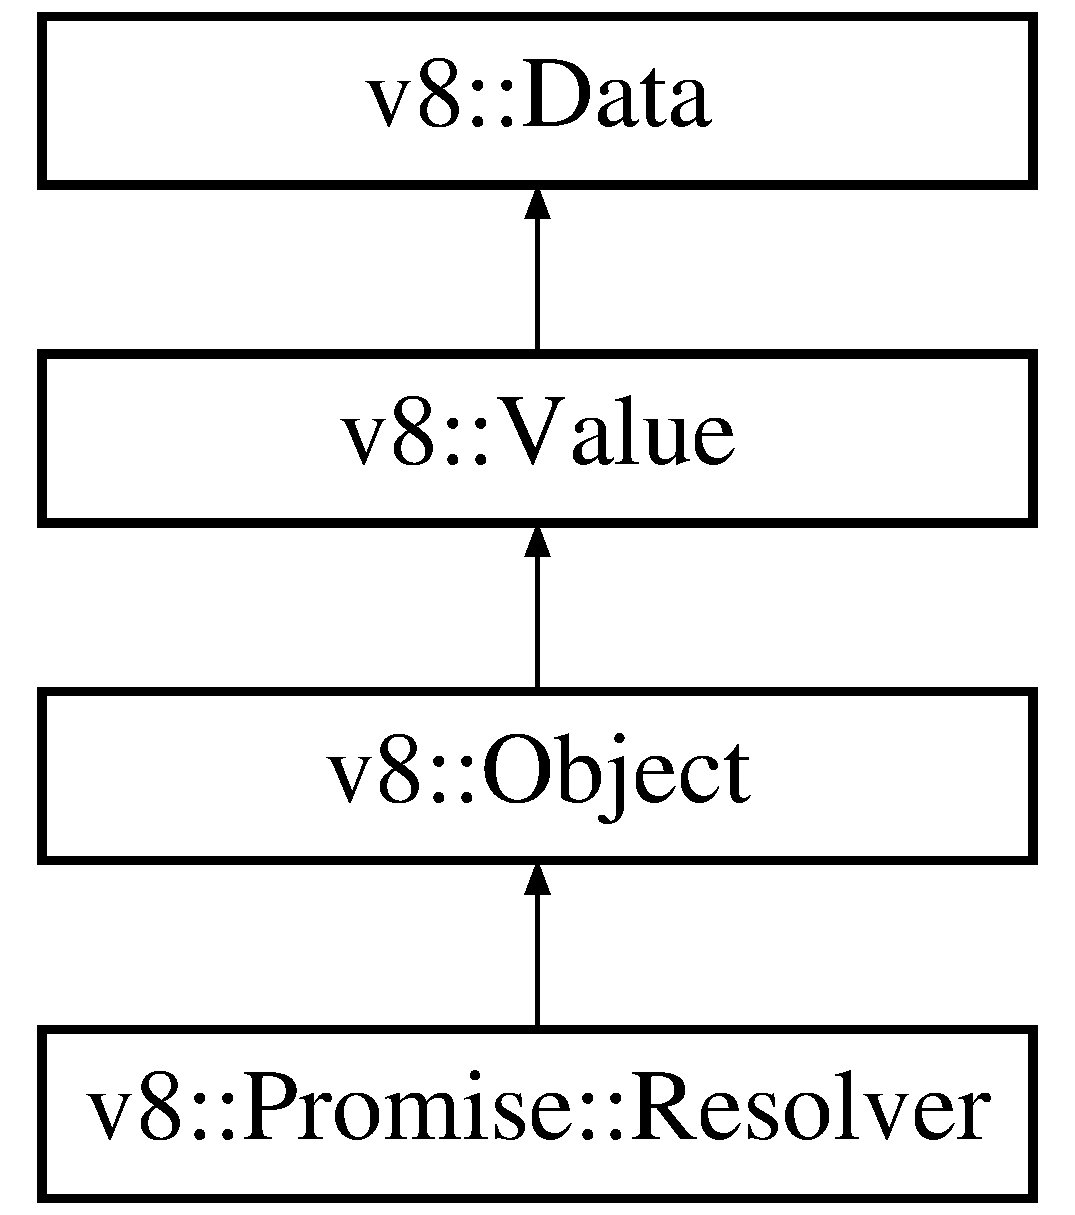
\includegraphics[height=4.000000cm]{classv8_1_1_promise_1_1_resolver}
\end{center}
\end{figure}
\subsection*{Public Member Functions}
\begin{DoxyCompactItemize}
\item 
\hyperlink{classv8_1_1_local}{Local}$<$ \hyperlink{classv8_1_1_promise}{Promise} $>$ \hyperlink{classv8_1_1_promise_1_1_resolver_a6f2f1c4d0d44d5c9cbf45404391fe83c}{Get\+Promise} ()
\item 
\hyperlink{classv8_1_1_promise_1_1_resolver_aff632d8369ba1198d0ce9f0072d278e7}{V8\+\_\+\+D\+E\+P\+R\+E\+C\+A\+T\+E\+\_\+\+S\+O\+ON} (\char`\"{}Use maybe version\char`\"{}, void Resolve(\hyperlink{classv8_1_1_local}{Local}$<$ \hyperlink{classv8_1_1_value}{Value} $>$ value))
\item 
\hyperlink{classv8_1_1_maybe}{Maybe}$<$ bool $>$ {\bfseries Resolve} (\hyperlink{classv8_1_1_local}{Local}$<$ \hyperlink{classv8_1_1_context}{Context} $>$ context, \hyperlink{classv8_1_1_local}{Local}$<$ \hyperlink{classv8_1_1_value}{Value} $>$ value)\hypertarget{classv8_1_1_promise_1_1_resolver_a95c37bf91e9ef02a2d3217730ebcf865}{}\label{classv8_1_1_promise_1_1_resolver_a95c37bf91e9ef02a2d3217730ebcf865}

\item 
{\bfseries V8\+\_\+\+D\+E\+P\+R\+E\+C\+A\+T\+E\+\_\+\+S\+O\+ON} (\char`\"{}Use maybe version\char`\"{}, void Reject(\hyperlink{classv8_1_1_local}{Local}$<$ \hyperlink{classv8_1_1_value}{Value} $>$ value))\hypertarget{classv8_1_1_promise_1_1_resolver_a56f20403d52528a8c06d8f3aa5fc1540}{}\label{classv8_1_1_promise_1_1_resolver_a56f20403d52528a8c06d8f3aa5fc1540}

\item 
\hyperlink{classv8_1_1_maybe}{Maybe}$<$ bool $>$ {\bfseries Reject} (\hyperlink{classv8_1_1_local}{Local}$<$ \hyperlink{classv8_1_1_context}{Context} $>$ context, \hyperlink{classv8_1_1_local}{Local}$<$ \hyperlink{classv8_1_1_value}{Value} $>$ value)\hypertarget{classv8_1_1_promise_1_1_resolver_ace0e84a6fcc93ac637a896d741b4432b}{}\label{classv8_1_1_promise_1_1_resolver_ace0e84a6fcc93ac637a896d741b4432b}

\end{DoxyCompactItemize}
\subsection*{Static Public Member Functions}
\begin{DoxyCompactItemize}
\item 
static \hyperlink{classv8_1_1_promise_1_1_resolver_a1aa04adcad6243802a3f9819fa840312}{V8\+\_\+\+D\+E\+P\+R\+E\+C\+A\+T\+E\+\_\+\+S\+O\+ON} (\char`\"{}Use maybe version\char`\"{}, Local$<$ \hyperlink{classv8_1_1_promise_1_1_resolver}{Resolver} $>$ New(\hyperlink{classv8_1_1_isolate}{Isolate} $\ast$isolate))
\item 
static V8\+\_\+\+W\+A\+R\+N\+\_\+\+U\+N\+U\+S\+E\+D\+\_\+\+R\+E\+S\+U\+LT \hyperlink{classv8_1_1_maybe_local}{Maybe\+Local}$<$ \hyperlink{classv8_1_1_promise_1_1_resolver}{Resolver} $>$ {\bfseries New} (\hyperlink{classv8_1_1_local}{Local}$<$ \hyperlink{classv8_1_1_context}{Context} $>$ context)\hypertarget{classv8_1_1_promise_1_1_resolver_a39a1f3acb070c85830aca527eebc3259}{}\label{classv8_1_1_promise_1_1_resolver_a39a1f3acb070c85830aca527eebc3259}

\item 
static V8\+\_\+\+I\+N\+L\+I\+NE \hyperlink{classv8_1_1_promise_1_1_resolver}{Resolver} $\ast$ {\bfseries Cast} (\hyperlink{classv8_1_1_value}{Value} $\ast$obj)\hypertarget{classv8_1_1_promise_1_1_resolver_ab2b541cb210158ed0c757c8b7dc46279}{}\label{classv8_1_1_promise_1_1_resolver_ab2b541cb210158ed0c757c8b7dc46279}

\end{DoxyCompactItemize}
\subsection*{Static Private Member Functions}
\begin{DoxyCompactItemize}
\item 
static void {\bfseries Check\+Cast} (\hyperlink{classv8_1_1_value}{Value} $\ast$obj)\hypertarget{classv8_1_1_promise_1_1_resolver_aa42133082f3d2952a6c9e3fe01668639}{}\label{classv8_1_1_promise_1_1_resolver_aa42133082f3d2952a6c9e3fe01668639}

\end{DoxyCompactItemize}


\subsection{Member Function Documentation}
\index{v8\+::\+Promise\+::\+Resolver@{v8\+::\+Promise\+::\+Resolver}!Get\+Promise@{Get\+Promise}}
\index{Get\+Promise@{Get\+Promise}!v8\+::\+Promise\+::\+Resolver@{v8\+::\+Promise\+::\+Resolver}}
\subsubsection[{\texorpdfstring{Get\+Promise()}{GetPromise()}}]{\setlength{\rightskip}{0pt plus 5cm}{\bf Local}$<$ {\bf Promise} $>$ v8\+::\+Promise\+::\+Resolver\+::\+Get\+Promise (
\begin{DoxyParamCaption}
{}
\end{DoxyParamCaption}
)}\hypertarget{classv8_1_1_promise_1_1_resolver_a6f2f1c4d0d44d5c9cbf45404391fe83c}{}\label{classv8_1_1_promise_1_1_resolver_a6f2f1c4d0d44d5c9cbf45404391fe83c}
Extract the associated promise. \index{v8\+::\+Promise\+::\+Resolver@{v8\+::\+Promise\+::\+Resolver}!V8\+\_\+\+D\+E\+P\+R\+E\+C\+A\+T\+E\+\_\+\+S\+O\+ON@{V8\+\_\+\+D\+E\+P\+R\+E\+C\+A\+T\+E\+\_\+\+S\+O\+ON}}
\index{V8\+\_\+\+D\+E\+P\+R\+E\+C\+A\+T\+E\+\_\+\+S\+O\+ON@{V8\+\_\+\+D\+E\+P\+R\+E\+C\+A\+T\+E\+\_\+\+S\+O\+ON}!v8\+::\+Promise\+::\+Resolver@{v8\+::\+Promise\+::\+Resolver}}
\subsubsection[{\texorpdfstring{V8\+\_\+\+D\+E\+P\+R\+E\+C\+A\+T\+E\+\_\+\+S\+O\+O\+N(""Use maybe version"", Local$<$ Resolver $>$ New(\+Isolate $\ast$isolate))}{V8_DEPRECATE_SOON("Use maybe version", Local< Resolver > New(Isolate *isolate))}}]{\setlength{\rightskip}{0pt plus 5cm}static v8\+::\+Promise\+::\+Resolver\+::\+V8\+\_\+\+D\+E\+P\+R\+E\+C\+A\+T\+E\+\_\+\+S\+O\+ON (
\begin{DoxyParamCaption}
\item[{\char`\"{}Use maybe version\char`\"{}}]{, }
\item[{{\bf Local}$<$ {\bf Resolver} $>$ }]{NewIsolate $\ast$isolate}
\end{DoxyParamCaption}
)\hspace{0.3cm}{\ttfamily [static]}}\hypertarget{classv8_1_1_promise_1_1_resolver_a1aa04adcad6243802a3f9819fa840312}{}\label{classv8_1_1_promise_1_1_resolver_a1aa04adcad6243802a3f9819fa840312}
Create a new resolver, along with an associated promise in pending state. \index{v8\+::\+Promise\+::\+Resolver@{v8\+::\+Promise\+::\+Resolver}!V8\+\_\+\+D\+E\+P\+R\+E\+C\+A\+T\+E\+\_\+\+S\+O\+ON@{V8\+\_\+\+D\+E\+P\+R\+E\+C\+A\+T\+E\+\_\+\+S\+O\+ON}}
\index{V8\+\_\+\+D\+E\+P\+R\+E\+C\+A\+T\+E\+\_\+\+S\+O\+ON@{V8\+\_\+\+D\+E\+P\+R\+E\+C\+A\+T\+E\+\_\+\+S\+O\+ON}!v8\+::\+Promise\+::\+Resolver@{v8\+::\+Promise\+::\+Resolver}}
\subsubsection[{\texorpdfstring{V8\+\_\+\+D\+E\+P\+R\+E\+C\+A\+T\+E\+\_\+\+S\+O\+O\+N(""Use maybe version"", void Resolve(\+Local$<$ Value $>$ value))}{V8_DEPRECATE_SOON("Use maybe version", void Resolve(Local< Value > value))}}]{\setlength{\rightskip}{0pt plus 5cm}v8\+::\+Promise\+::\+Resolver\+::\+V8\+\_\+\+D\+E\+P\+R\+E\+C\+A\+T\+E\+\_\+\+S\+O\+ON (
\begin{DoxyParamCaption}
\item[{\char`\"{}Use maybe version\char`\"{}}]{, }
\item[{void }]{ResolveLocal$<$ Value $>$ value}
\end{DoxyParamCaption}
)}\hypertarget{classv8_1_1_promise_1_1_resolver_aff632d8369ba1198d0ce9f0072d278e7}{}\label{classv8_1_1_promise_1_1_resolver_aff632d8369ba1198d0ce9f0072d278e7}
Resolve/reject the associated promise with a given value. Ignored if the promise is no longer pending. 

The documentation for this class was generated from the following files\+:\begin{DoxyCompactItemize}
\item 
/\+Users/joshgav/node/v8/include/v8.\+h\item 
/\+Users/joshgav/node/v8/src/api.\+cc\end{DoxyCompactItemize}

\hypertarget{classv8_1_1_resource_constraints}{}\section{v8\+:\+:Resource\+Constraints Class Reference}
\label{classv8_1_1_resource_constraints}\index{v8\+::\+Resource\+Constraints@{v8\+::\+Resource\+Constraints}}


{\ttfamily \#include $<$v8.\+h$>$}

\subsection*{Public Member Functions}
\begin{DoxyCompactItemize}
\item 
void \hyperlink{classv8_1_1_resource_constraints_aeeaaee4017e8d5f8f0439af2af2ed3a5}{Configure\+Defaults} (uint64\+\_\+t physical\+\_\+memory, uint64\+\_\+t virtual\+\_\+memory\+\_\+limit)
\item 
int {\bfseries max\+\_\+semi\+\_\+space\+\_\+size} () const \hypertarget{classv8_1_1_resource_constraints_aeeecbbdb2c7880bf74d5d7fb9bbc52b3}{}\label{classv8_1_1_resource_constraints_aeeecbbdb2c7880bf74d5d7fb9bbc52b3}

\item 
void {\bfseries set\+\_\+max\+\_\+semi\+\_\+space\+\_\+size} (int limit\+\_\+in\+\_\+mb)\hypertarget{classv8_1_1_resource_constraints_abee8b1156cbba22f09c4fc553b0a34f3}{}\label{classv8_1_1_resource_constraints_abee8b1156cbba22f09c4fc553b0a34f3}

\item 
int {\bfseries max\+\_\+old\+\_\+space\+\_\+size} () const \hypertarget{classv8_1_1_resource_constraints_a72840efdbcfc7bb287c6aea38d0b07b9}{}\label{classv8_1_1_resource_constraints_a72840efdbcfc7bb287c6aea38d0b07b9}

\item 
void {\bfseries set\+\_\+max\+\_\+old\+\_\+space\+\_\+size} (int limit\+\_\+in\+\_\+mb)\hypertarget{classv8_1_1_resource_constraints_a54307a3e64cb7e0198b3a137dddd5965}{}\label{classv8_1_1_resource_constraints_a54307a3e64cb7e0198b3a137dddd5965}

\item 
int {\bfseries max\+\_\+executable\+\_\+size} () const \hypertarget{classv8_1_1_resource_constraints_a037777e608ed1c22fe294ecef5722036}{}\label{classv8_1_1_resource_constraints_a037777e608ed1c22fe294ecef5722036}

\item 
void {\bfseries set\+\_\+max\+\_\+executable\+\_\+size} (int limit\+\_\+in\+\_\+mb)\hypertarget{classv8_1_1_resource_constraints_a2f1ac501d324d6b3d06463c4d6a5c242}{}\label{classv8_1_1_resource_constraints_a2f1ac501d324d6b3d06463c4d6a5c242}

\item 
uint32\+\_\+t $\ast$ {\bfseries stack\+\_\+limit} () const \hypertarget{classv8_1_1_resource_constraints_aafc4a94f2eeb0684e7a50f355eb4d06d}{}\label{classv8_1_1_resource_constraints_aafc4a94f2eeb0684e7a50f355eb4d06d}

\item 
void {\bfseries set\+\_\+stack\+\_\+limit} (uint32\+\_\+t $\ast$value)\hypertarget{classv8_1_1_resource_constraints_a26ed3e89985a4afe34e84509fb093cf1}{}\label{classv8_1_1_resource_constraints_a26ed3e89985a4afe34e84509fb093cf1}

\item 
size\+\_\+t {\bfseries code\+\_\+range\+\_\+size} () const \hypertarget{classv8_1_1_resource_constraints_a8dd511917ad17bf2185d574b0c7e4186}{}\label{classv8_1_1_resource_constraints_a8dd511917ad17bf2185d574b0c7e4186}

\item 
void {\bfseries set\+\_\+code\+\_\+range\+\_\+size} (size\+\_\+t limit\+\_\+in\+\_\+mb)\hypertarget{classv8_1_1_resource_constraints_adeab824b969292881098b66164ab9e13}{}\label{classv8_1_1_resource_constraints_adeab824b969292881098b66164ab9e13}

\end{DoxyCompactItemize}
\subsection*{Private Attributes}
\begin{DoxyCompactItemize}
\item 
int {\bfseries max\+\_\+semi\+\_\+space\+\_\+size\+\_\+}\hypertarget{classv8_1_1_resource_constraints_a86c60a00594dc8fbd5944b6828b2d6c8}{}\label{classv8_1_1_resource_constraints_a86c60a00594dc8fbd5944b6828b2d6c8}

\item 
int {\bfseries max\+\_\+old\+\_\+space\+\_\+size\+\_\+}\hypertarget{classv8_1_1_resource_constraints_ada39b1b3247ba65aa93ee9b6c8f4d92c}{}\label{classv8_1_1_resource_constraints_ada39b1b3247ba65aa93ee9b6c8f4d92c}

\item 
int {\bfseries max\+\_\+executable\+\_\+size\+\_\+}\hypertarget{classv8_1_1_resource_constraints_aa796ecd10206ccdcd38cde3087383ef4}{}\label{classv8_1_1_resource_constraints_aa796ecd10206ccdcd38cde3087383ef4}

\item 
uint32\+\_\+t $\ast$ {\bfseries stack\+\_\+limit\+\_\+}\hypertarget{classv8_1_1_resource_constraints_a0b2084c6e0c3f857410d0f9326d7c5af}{}\label{classv8_1_1_resource_constraints_a0b2084c6e0c3f857410d0f9326d7c5af}

\item 
size\+\_\+t {\bfseries code\+\_\+range\+\_\+size\+\_\+}\hypertarget{classv8_1_1_resource_constraints_ada688048046ed92c3efa99169541b8e3}{}\label{classv8_1_1_resource_constraints_ada688048046ed92c3efa99169541b8e3}

\end{DoxyCompactItemize}


\subsection{Detailed Description}
A set of constraints that specifies the limits of the runtime\textquotesingle{}s memory use. You must set the heap size before initializing the VM -\/ the size cannot be adjusted after the VM is initialized.

If you are using threads then you should hold the V8\+::\+Locker lock while setting the stack limit and you must set a non-\/default stack limit separately for each thread.

The arguments for set\+\_\+max\+\_\+semi\+\_\+space\+\_\+size, set\+\_\+max\+\_\+old\+\_\+space\+\_\+size, set\+\_\+max\+\_\+executable\+\_\+size, set\+\_\+code\+\_\+range\+\_\+size specify limits in MB. 

\subsection{Member Function Documentation}
\index{v8\+::\+Resource\+Constraints@{v8\+::\+Resource\+Constraints}!Configure\+Defaults@{Configure\+Defaults}}
\index{Configure\+Defaults@{Configure\+Defaults}!v8\+::\+Resource\+Constraints@{v8\+::\+Resource\+Constraints}}
\subsubsection[{\texorpdfstring{Configure\+Defaults(uint64\+\_\+t physical\+\_\+memory, uint64\+\_\+t virtual\+\_\+memory\+\_\+limit)}{ConfigureDefaults(uint64_t physical_memory, uint64_t virtual_memory_limit)}}]{\setlength{\rightskip}{0pt plus 5cm}void v8\+::\+Resource\+Constraints\+::\+Configure\+Defaults (
\begin{DoxyParamCaption}
\item[{uint64\+\_\+t}]{physical\+\_\+memory, }
\item[{uint64\+\_\+t}]{virtual\+\_\+memory\+\_\+limit}
\end{DoxyParamCaption}
)}\hypertarget{classv8_1_1_resource_constraints_aeeaaee4017e8d5f8f0439af2af2ed3a5}{}\label{classv8_1_1_resource_constraints_aeeaaee4017e8d5f8f0439af2af2ed3a5}
Configures the constraints with reasonable default values based on the capabilities of the current device the VM is running on.


\begin{DoxyParams}{Parameters}
{\em physical\+\_\+memory} & The total amount of physical memory on the current device, in bytes. \\
\hline
{\em virtual\+\_\+memory\+\_\+limit} & The amount of virtual memory on the current device, in bytes, or zero, if there is no limit. \\
\hline
\end{DoxyParams}


The documentation for this class was generated from the following file\+:\begin{DoxyCompactItemize}
\item 
include/v8.\+h\end{DoxyCompactItemize}

\hypertarget{classv8_1_1_retained_object_info}{}\section{v8\+:\+:Retained\+Object\+Info Class Reference}
\label{classv8_1_1_retained_object_info}\index{v8\+::\+Retained\+Object\+Info@{v8\+::\+Retained\+Object\+Info}}


{\ttfamily \#include $<$v8-\/profiler.\+h$>$}

Inheritance diagram for v8\+:\+:Retained\+Object\+Info\+:\begin{figure}[H]
\begin{center}
\leavevmode
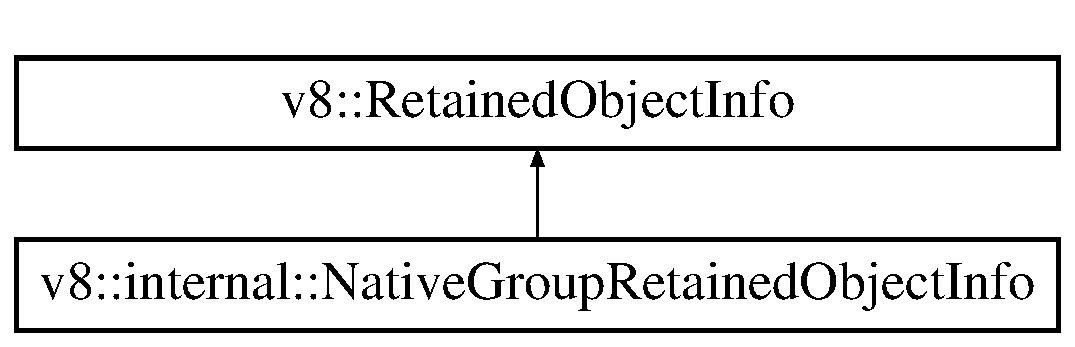
\includegraphics[height=2.000000cm]{classv8_1_1_retained_object_info}
\end{center}
\end{figure}
\subsection*{Public Member Functions}
\begin{DoxyCompactItemize}
\item 
virtual void \hyperlink{classv8_1_1_retained_object_info_a5011203f7c5949049ba36b8059f03eca}{Dispose} ()=0
\item 
virtual bool \hyperlink{classv8_1_1_retained_object_info_a286103bb076c85415919c86b1838c990}{Is\+Equivalent} (\hyperlink{classv8_1_1_retained_object_info}{Retained\+Object\+Info} $\ast$other)=0
\item 
virtual intptr\+\_\+t \hyperlink{classv8_1_1_retained_object_info_a6fdbfa242b95615e63f08433419c8066}{Get\+Hash} ()=0
\item 
virtual const char $\ast$ \hyperlink{classv8_1_1_retained_object_info_ad19106fc7f0499fd45005077551d54c0}{Get\+Label} ()=0
\item 
virtual const char $\ast$ \hyperlink{classv8_1_1_retained_object_info_adf835370c5516f2a89dd2d3f83dee10b}{Get\+Group\+Label} ()
\item 
virtual intptr\+\_\+t \hyperlink{classv8_1_1_retained_object_info_ae6865597469bc7d28bd8ec71b4b890bd}{Get\+Element\+Count} ()
\item 
virtual intptr\+\_\+t \hyperlink{classv8_1_1_retained_object_info_a1a899eed0b1f6e046edc3c7a7c08aa8c}{Get\+Size\+In\+Bytes} ()
\end{DoxyCompactItemize}
\subsection*{Private Member Functions}
\begin{DoxyCompactItemize}
\item 
{\bfseries Retained\+Object\+Info} (const \hyperlink{classv8_1_1_retained_object_info}{Retained\+Object\+Info} \&)\hypertarget{classv8_1_1_retained_object_info_af2d2af908d53a2e4e2f543b7c67057c8}{}\label{classv8_1_1_retained_object_info_af2d2af908d53a2e4e2f543b7c67057c8}

\item 
\hyperlink{classv8_1_1_retained_object_info}{Retained\+Object\+Info} \& {\bfseries operator=} (const \hyperlink{classv8_1_1_retained_object_info}{Retained\+Object\+Info} \&)\hypertarget{classv8_1_1_retained_object_info_a11fcc91279bee920e05e217c77f78eed}{}\label{classv8_1_1_retained_object_info_a11fcc91279bee920e05e217c77f78eed}

\end{DoxyCompactItemize}


\subsection{Detailed Description}
Interface for providing information about embedder\textquotesingle{}s objects held by global handles. This information is reported in two ways\+:


\begin{DoxyEnumerate}
\item When calling Add\+Object\+Group, an embedder may pass \hyperlink{classv8_1_1_retained_object_info}{Retained\+Object\+Info} instance describing the group. To collect this information while taking a heap snapshot, \hyperlink{classv8_1_1_v8}{V8} calls GC prologue and epilogue callbacks.
\item When a heap snapshot is collected, \hyperlink{classv8_1_1_v8}{V8} additionally requests Retained\+Object\+Infos for persistent handles that were not previously reported via Add\+Object\+Group.
\end{DoxyEnumerate}

Thus, if an embedder wants to provide information about native objects for heap snapshots, he can do it in a GC prologue handler, and / or by assigning wrapper class ids in the following way\+:


\begin{DoxyEnumerate}
\item Bind a callback to class id by calling Set\+Wrapper\+Class\+Info\+Provider.
\item Call Set\+Wrapper\+Class\+Id on certain persistent handles.
\end{DoxyEnumerate}

\hyperlink{classv8_1_1_v8}{V8} takes ownership of \hyperlink{classv8_1_1_retained_object_info}{Retained\+Object\+Info} instances passed to it and keeps them alive only during snapshot collection. Afterwards, they are freed by calling the Dispose class function. 

\subsection{Member Function Documentation}
\index{v8\+::\+Retained\+Object\+Info@{v8\+::\+Retained\+Object\+Info}!Dispose@{Dispose}}
\index{Dispose@{Dispose}!v8\+::\+Retained\+Object\+Info@{v8\+::\+Retained\+Object\+Info}}
\subsubsection[{\texorpdfstring{Dispose()=0}{Dispose()=0}}]{\setlength{\rightskip}{0pt plus 5cm}virtual void v8\+::\+Retained\+Object\+Info\+::\+Dispose (
\begin{DoxyParamCaption}
{}
\end{DoxyParamCaption}
)\hspace{0.3cm}{\ttfamily [pure virtual]}}\hypertarget{classv8_1_1_retained_object_info_a5011203f7c5949049ba36b8059f03eca}{}\label{classv8_1_1_retained_object_info_a5011203f7c5949049ba36b8059f03eca}
Called by \hyperlink{classv8_1_1_v8}{V8} when it no longer needs an instance. 

Implemented in \hyperlink{classv8_1_1internal_1_1_native_group_retained_object_info_aaea81e04752da6a0e273b5349e40c2d8}{v8\+::internal\+::\+Native\+Group\+Retained\+Object\+Info}.

\index{v8\+::\+Retained\+Object\+Info@{v8\+::\+Retained\+Object\+Info}!Get\+Element\+Count@{Get\+Element\+Count}}
\index{Get\+Element\+Count@{Get\+Element\+Count}!v8\+::\+Retained\+Object\+Info@{v8\+::\+Retained\+Object\+Info}}
\subsubsection[{\texorpdfstring{Get\+Element\+Count()}{GetElementCount()}}]{\setlength{\rightskip}{0pt plus 5cm}virtual intptr\+\_\+t v8\+::\+Retained\+Object\+Info\+::\+Get\+Element\+Count (
\begin{DoxyParamCaption}
{}
\end{DoxyParamCaption}
)\hspace{0.3cm}{\ttfamily [inline]}, {\ttfamily [virtual]}}\hypertarget{classv8_1_1_retained_object_info_ae6865597469bc7d28bd8ec71b4b890bd}{}\label{classv8_1_1_retained_object_info_ae6865597469bc7d28bd8ec71b4b890bd}
Returns element count in case if a global handle retains a subgraph by holding one of its nodes. \index{v8\+::\+Retained\+Object\+Info@{v8\+::\+Retained\+Object\+Info}!Get\+Group\+Label@{Get\+Group\+Label}}
\index{Get\+Group\+Label@{Get\+Group\+Label}!v8\+::\+Retained\+Object\+Info@{v8\+::\+Retained\+Object\+Info}}
\subsubsection[{\texorpdfstring{Get\+Group\+Label()}{GetGroupLabel()}}]{\setlength{\rightskip}{0pt plus 5cm}virtual const char$\ast$ v8\+::\+Retained\+Object\+Info\+::\+Get\+Group\+Label (
\begin{DoxyParamCaption}
{}
\end{DoxyParamCaption}
)\hspace{0.3cm}{\ttfamily [inline]}, {\ttfamily [virtual]}}\hypertarget{classv8_1_1_retained_object_info_adf835370c5516f2a89dd2d3f83dee10b}{}\label{classv8_1_1_retained_object_info_adf835370c5516f2a89dd2d3f83dee10b}
Returns human-\/readable group label. It must be a null-\/terminated U\+T\+F-\/8 encoded string. \hyperlink{classv8_1_1_v8}{V8} copies its contents during a call to Get\+Group\+Label. Heap snapshot generator will collect all the group names, create top level entries with these names and attach the objects to the corresponding top level group objects. There is a default implementation which is required because embedders don\textquotesingle{}t have their own implementation yet. \index{v8\+::\+Retained\+Object\+Info@{v8\+::\+Retained\+Object\+Info}!Get\+Hash@{Get\+Hash}}
\index{Get\+Hash@{Get\+Hash}!v8\+::\+Retained\+Object\+Info@{v8\+::\+Retained\+Object\+Info}}
\subsubsection[{\texorpdfstring{Get\+Hash()=0}{GetHash()=0}}]{\setlength{\rightskip}{0pt plus 5cm}virtual intptr\+\_\+t v8\+::\+Retained\+Object\+Info\+::\+Get\+Hash (
\begin{DoxyParamCaption}
{}
\end{DoxyParamCaption}
)\hspace{0.3cm}{\ttfamily [pure virtual]}}\hypertarget{classv8_1_1_retained_object_info_a6fdbfa242b95615e63f08433419c8066}{}\label{classv8_1_1_retained_object_info_a6fdbfa242b95615e63f08433419c8066}
Returns hash value for the instance. Equivalent instances must have the same hash value. 

Implemented in \hyperlink{classv8_1_1internal_1_1_native_group_retained_object_info_a27593c16a13464c40f097f1bfaddcc66}{v8\+::internal\+::\+Native\+Group\+Retained\+Object\+Info}.

\index{v8\+::\+Retained\+Object\+Info@{v8\+::\+Retained\+Object\+Info}!Get\+Label@{Get\+Label}}
\index{Get\+Label@{Get\+Label}!v8\+::\+Retained\+Object\+Info@{v8\+::\+Retained\+Object\+Info}}
\subsubsection[{\texorpdfstring{Get\+Label()=0}{GetLabel()=0}}]{\setlength{\rightskip}{0pt plus 5cm}virtual const char$\ast$ v8\+::\+Retained\+Object\+Info\+::\+Get\+Label (
\begin{DoxyParamCaption}
{}
\end{DoxyParamCaption}
)\hspace{0.3cm}{\ttfamily [pure virtual]}}\hypertarget{classv8_1_1_retained_object_info_ad19106fc7f0499fd45005077551d54c0}{}\label{classv8_1_1_retained_object_info_ad19106fc7f0499fd45005077551d54c0}
Returns human-\/readable label. It must be a null-\/terminated U\+T\+F-\/8 encoded string. \hyperlink{classv8_1_1_v8}{V8} copies its contents during a call to Get\+Label. 

Implemented in \hyperlink{classv8_1_1internal_1_1_native_group_retained_object_info_a794dc2fa2541c4786953f567ea1d1990}{v8\+::internal\+::\+Native\+Group\+Retained\+Object\+Info}.

\index{v8\+::\+Retained\+Object\+Info@{v8\+::\+Retained\+Object\+Info}!Get\+Size\+In\+Bytes@{Get\+Size\+In\+Bytes}}
\index{Get\+Size\+In\+Bytes@{Get\+Size\+In\+Bytes}!v8\+::\+Retained\+Object\+Info@{v8\+::\+Retained\+Object\+Info}}
\subsubsection[{\texorpdfstring{Get\+Size\+In\+Bytes()}{GetSizeInBytes()}}]{\setlength{\rightskip}{0pt plus 5cm}virtual intptr\+\_\+t v8\+::\+Retained\+Object\+Info\+::\+Get\+Size\+In\+Bytes (
\begin{DoxyParamCaption}
{}
\end{DoxyParamCaption}
)\hspace{0.3cm}{\ttfamily [inline]}, {\ttfamily [virtual]}}\hypertarget{classv8_1_1_retained_object_info_a1a899eed0b1f6e046edc3c7a7c08aa8c}{}\label{classv8_1_1_retained_object_info_a1a899eed0b1f6e046edc3c7a7c08aa8c}
Returns embedder\textquotesingle{}s object size in bytes. \index{v8\+::\+Retained\+Object\+Info@{v8\+::\+Retained\+Object\+Info}!Is\+Equivalent@{Is\+Equivalent}}
\index{Is\+Equivalent@{Is\+Equivalent}!v8\+::\+Retained\+Object\+Info@{v8\+::\+Retained\+Object\+Info}}
\subsubsection[{\texorpdfstring{Is\+Equivalent(\+Retained\+Object\+Info $\ast$other)=0}{IsEquivalent(RetainedObjectInfo *other)=0}}]{\setlength{\rightskip}{0pt plus 5cm}virtual bool v8\+::\+Retained\+Object\+Info\+::\+Is\+Equivalent (
\begin{DoxyParamCaption}
\item[{{\bf Retained\+Object\+Info} $\ast$}]{other}
\end{DoxyParamCaption}
)\hspace{0.3cm}{\ttfamily [pure virtual]}}\hypertarget{classv8_1_1_retained_object_info_a286103bb076c85415919c86b1838c990}{}\label{classv8_1_1_retained_object_info_a286103bb076c85415919c86b1838c990}
Returns whether two instances are equivalent. 

Implemented in \hyperlink{classv8_1_1internal_1_1_native_group_retained_object_info_a6c6bbdecc0a199cd5a79520161d02a1f}{v8\+::internal\+::\+Native\+Group\+Retained\+Object\+Info}.



The documentation for this class was generated from the following file\+:\begin{DoxyCompactItemize}
\item 
/\+Users/joshgav/node/v8/include/v8-\/profiler.\+h\end{DoxyCompactItemize}

\hypertarget{classv8_1_1_return_value}{}\section{v8\+:\+:Return\+Value$<$ T $>$ Class Template Reference}
\label{classv8_1_1_return_value}\index{v8\+::\+Return\+Value$<$ T $>$@{v8\+::\+Return\+Value$<$ T $>$}}
\subsection*{Public Member Functions}
\begin{DoxyCompactItemize}
\item 
{\footnotesize template$<$class S $>$ }\\V8\+\_\+\+I\+N\+L\+I\+NE {\bfseries Return\+Value} (const \hyperlink{classv8_1_1_return_value}{Return\+Value}$<$ S $>$ \&that)\hypertarget{classv8_1_1_return_value_a0f1cdf01090e6fc957a0081036a55e6b}{}\label{classv8_1_1_return_value_a0f1cdf01090e6fc957a0081036a55e6b}

\item 
{\footnotesize template$<$typename S $>$ }\\V8\+\_\+\+I\+N\+L\+I\+NE {\bfseries V8\+\_\+\+D\+E\+P\+R\+E\+C\+A\+T\+E\+\_\+\+S\+O\+ON} (\char`\"{}Use \hyperlink{classv8_1_1_global}{Global}$<$$>$ instead\char`\"{}, void \hyperlink{classv8_1_1_set}{Set}(const \hyperlink{classv8_1_1_persistent}{Persistent}$<$ S $>$ \&handle))\hypertarget{classv8_1_1_return_value_a852de19bf776c8ed9b5a0c40abe1f011}{}\label{classv8_1_1_return_value_a852de19bf776c8ed9b5a0c40abe1f011}

\item 
{\footnotesize template$<$typename S $>$ }\\V8\+\_\+\+I\+N\+L\+I\+NE void {\bfseries Set} (const \hyperlink{classv8_1_1_global}{Global}$<$ S $>$ \&handle)\hypertarget{classv8_1_1_return_value_acd7bacd0c0c42de6d7bc904b66fab5d6}{}\label{classv8_1_1_return_value_acd7bacd0c0c42de6d7bc904b66fab5d6}

\item 
{\footnotesize template$<$typename S $>$ }\\V8\+\_\+\+I\+N\+L\+I\+NE void {\bfseries Set} (const \hyperlink{classv8_1_1_local}{Local}$<$ S $>$ handle)\hypertarget{classv8_1_1_return_value_a865bc8fbded0b17338d7109d8e63be7b}{}\label{classv8_1_1_return_value_a865bc8fbded0b17338d7109d8e63be7b}

\item 
V8\+\_\+\+I\+N\+L\+I\+NE void {\bfseries Set} (bool value)\hypertarget{classv8_1_1_return_value_a74d13d68c48028d14934cf076b21fa70}{}\label{classv8_1_1_return_value_a74d13d68c48028d14934cf076b21fa70}

\item 
V8\+\_\+\+I\+N\+L\+I\+NE void {\bfseries Set} (double i)\hypertarget{classv8_1_1_return_value_a28bc181b8f64fd21a331bf42d97fe41f}{}\label{classv8_1_1_return_value_a28bc181b8f64fd21a331bf42d97fe41f}

\item 
V8\+\_\+\+I\+N\+L\+I\+NE void {\bfseries Set} (int32\+\_\+t i)\hypertarget{classv8_1_1_return_value_ab214555052e3d03b8c44a7e8779bcbc2}{}\label{classv8_1_1_return_value_ab214555052e3d03b8c44a7e8779bcbc2}

\item 
V8\+\_\+\+I\+N\+L\+I\+NE void {\bfseries Set} (uint32\+\_\+t i)\hypertarget{classv8_1_1_return_value_a9e190fff3c0396656e752ee916c715dc}{}\label{classv8_1_1_return_value_a9e190fff3c0396656e752ee916c715dc}

\item 
V8\+\_\+\+I\+N\+L\+I\+NE void {\bfseries Set\+Null} ()\hypertarget{classv8_1_1_return_value_aba8480ee94ea905ad0850b3ceaf1b9b1}{}\label{classv8_1_1_return_value_aba8480ee94ea905ad0850b3ceaf1b9b1}

\item 
V8\+\_\+\+I\+N\+L\+I\+NE void {\bfseries Set\+Undefined} ()\hypertarget{classv8_1_1_return_value_af73d4ed15f126a214efe583ac56ff19d}{}\label{classv8_1_1_return_value_af73d4ed15f126a214efe583ac56ff19d}

\item 
V8\+\_\+\+I\+N\+L\+I\+NE void {\bfseries Set\+Empty\+String} ()\hypertarget{classv8_1_1_return_value_a3ed4f59f726eafae53525bb68512b93e}{}\label{classv8_1_1_return_value_a3ed4f59f726eafae53525bb68512b93e}

\item 
V8\+\_\+\+I\+N\+L\+I\+NE \hyperlink{classv8_1_1_isolate}{Isolate} $\ast$ {\bfseries Get\+Isolate} () const \hypertarget{classv8_1_1_return_value_a2d2ad61afb973f95b47103f7f555762f}{}\label{classv8_1_1_return_value_a2d2ad61afb973f95b47103f7f555762f}

\item 
{\footnotesize template$<$typename S $>$ }\\V8\+\_\+\+I\+N\+L\+I\+NE void {\bfseries Set} (S $\ast$whatever)\hypertarget{classv8_1_1_return_value_acbfa5f2c7cf2e95b42a4dcf79874fbe5}{}\label{classv8_1_1_return_value_acbfa5f2c7cf2e95b42a4dcf79874fbe5}

\item 
V8\+\_\+\+I\+N\+L\+I\+NE \hyperlink{classv8_1_1_local}{Local}$<$ \hyperlink{classv8_1_1_value}{Value} $>$ {\bfseries Get} () const \hypertarget{classv8_1_1_return_value_aa4e6596d19788787dac914ba4eaecb4d}{}\label{classv8_1_1_return_value_aa4e6596d19788787dac914ba4eaecb4d}

\item 
{\footnotesize template$<$typename S $>$ }\\void {\bfseries Set} (const \hyperlink{classv8_1_1_persistent}{Persistent}$<$ S $>$ \&handle)\hypertarget{classv8_1_1_return_value_a2ff02f4be7d7fdcf0e21be43dfd4fe43}{}\label{classv8_1_1_return_value_a2ff02f4be7d7fdcf0e21be43dfd4fe43}

\item 
{\footnotesize template$<$typename S $>$ }\\void {\bfseries Set} (const \hyperlink{classv8_1_1_global}{Global}$<$ S $>$ \&handle)\hypertarget{classv8_1_1_return_value_a57c4b962cf2ca387d3fb9a2f8e47a963}{}\label{classv8_1_1_return_value_a57c4b962cf2ca387d3fb9a2f8e47a963}

\item 
{\footnotesize template$<$typename S $>$ }\\void {\bfseries Set} (const \hyperlink{classv8_1_1_local}{Local}$<$ S $>$ handle)\hypertarget{classv8_1_1_return_value_a69d99ab0e0c12d68291d425287532799}{}\label{classv8_1_1_return_value_a69d99ab0e0c12d68291d425287532799}

\item 
{\footnotesize template$<$typename S $>$ }\\void {\bfseries Set} (S $\ast$whatever)\hypertarget{classv8_1_1_return_value_a766f60aa4d7d86bfb949d3c40b147ef7}{}\label{classv8_1_1_return_value_a766f60aa4d7d86bfb949d3c40b147ef7}

\end{DoxyCompactItemize}
\subsection*{Private Member Functions}
\begin{DoxyCompactItemize}
\item 
V8\+\_\+\+I\+N\+L\+I\+NE void {\bfseries Set\+Internal} (internal\+::\+Object $\ast$value)\hypertarget{classv8_1_1_return_value_a364b24a88d730fc7fd0eab0e7c3cd708}{}\label{classv8_1_1_return_value_a364b24a88d730fc7fd0eab0e7c3cd708}

\item 
V8\+\_\+\+I\+N\+L\+I\+NE internal\+::\+Object $\ast$ {\bfseries Get\+Default\+Value} ()\hypertarget{classv8_1_1_return_value_af30c5efde16a4242b10c9d9a01a8ddff}{}\label{classv8_1_1_return_value_af30c5efde16a4242b10c9d9a01a8ddff}

\item 
V8\+\_\+\+I\+N\+L\+I\+NE {\bfseries Return\+Value} (internal\+::\+Object $\ast$$\ast$slot)\hypertarget{classv8_1_1_return_value_ae696ba3e11a56243aa19f8875e71b72c}{}\label{classv8_1_1_return_value_ae696ba3e11a56243aa19f8875e71b72c}

\end{DoxyCompactItemize}
\subsection*{Private Attributes}
\begin{DoxyCompactItemize}
\item 
internal\+::\+Object $\ast$$\ast$ {\bfseries value\+\_\+}\hypertarget{classv8_1_1_return_value_abb24c21d81cd11d48a5f3872529702a7}{}\label{classv8_1_1_return_value_abb24c21d81cd11d48a5f3872529702a7}

\end{DoxyCompactItemize}
\subsection*{Friends}
\begin{DoxyCompactItemize}
\item 
{\footnotesize template$<$class F $>$ }\\class {\bfseries Return\+Value}\hypertarget{classv8_1_1_return_value_a53f604d3d6f2dc0647df33c9979f116a}{}\label{classv8_1_1_return_value_a53f604d3d6f2dc0647df33c9979f116a}

\item 
{\footnotesize template$<$class F $>$ }\\class {\bfseries Function\+Callback\+Info}\hypertarget{classv8_1_1_return_value_a76786e6fa2d0eac5e2d4f647659d0d23}{}\label{classv8_1_1_return_value_a76786e6fa2d0eac5e2d4f647659d0d23}

\item 
{\footnotesize template$<$class F $>$ }\\class {\bfseries Property\+Callback\+Info}\hypertarget{classv8_1_1_return_value_a5018adab21fade2b42f4f60e45fa1083}{}\label{classv8_1_1_return_value_a5018adab21fade2b42f4f60e45fa1083}

\item 
{\footnotesize template$<$class F , class G , class H $>$ }\\class {\bfseries Persistent\+Value\+Map\+Base}\hypertarget{classv8_1_1_return_value_a08e2b8f164392d71811ce6cc134f33e3}{}\label{classv8_1_1_return_value_a08e2b8f164392d71811ce6cc134f33e3}

\end{DoxyCompactItemize}


The documentation for this class was generated from the following file\+:\begin{DoxyCompactItemize}
\item 
/\+Users/joshgav/node/v8/include/v8.\+h\end{DoxyCompactItemize}

\hypertarget{structv8_1_1_sample_info}{}\section{v8\+:\+:Sample\+Info Struct Reference}
\label{structv8_1_1_sample_info}\index{v8\+::\+Sample\+Info@{v8\+::\+Sample\+Info}}
\subsection*{Public Attributes}
\begin{DoxyCompactItemize}
\item 
size\+\_\+t {\bfseries frames\+\_\+count}\hypertarget{structv8_1_1_sample_info_a5f1e51bc358605e0c1d38fb2f3d344cd}{}\label{structv8_1_1_sample_info_a5f1e51bc358605e0c1d38fb2f3d344cd}

\item 
State\+Tag {\bfseries vm\+\_\+state}\hypertarget{structv8_1_1_sample_info_afd6198c9feb44a8df79576cf427b9a91}{}\label{structv8_1_1_sample_info_afd6198c9feb44a8df79576cf427b9a91}

\end{DoxyCompactItemize}


The documentation for this struct was generated from the following file\+:\begin{DoxyCompactItemize}
\item 
include/v8.\+h\end{DoxyCompactItemize}

\hypertarget{classv8_1_1_isolate_1_1_scope}{}\section{v8\+:\+:Isolate\+:\+:Scope Class Reference}
\label{classv8_1_1_isolate_1_1_scope}\index{v8\+::\+Isolate\+::\+Scope@{v8\+::\+Isolate\+::\+Scope}}


{\ttfamily \#include $<$v8.\+h$>$}

\subsection*{Public Member Functions}
\begin{DoxyCompactItemize}
\item 
{\bfseries Scope} (\hyperlink{classv8_1_1_isolate}{Isolate} $\ast$isolate)\hypertarget{classv8_1_1_isolate_1_1_scope_a43889336478a5625e095c4444b9dd684}{}\label{classv8_1_1_isolate_1_1_scope_a43889336478a5625e095c4444b9dd684}

\end{DoxyCompactItemize}
\subsection*{Private Member Functions}
\begin{DoxyCompactItemize}
\item 
{\bfseries Scope} (const \hyperlink{classv8_1_1_isolate_1_1_scope}{Scope} \&)\hypertarget{classv8_1_1_isolate_1_1_scope_aeda42aa2368c6457501d93b6b49f7a59}{}\label{classv8_1_1_isolate_1_1_scope_aeda42aa2368c6457501d93b6b49f7a59}

\item 
\hyperlink{classv8_1_1_isolate_1_1_scope}{Scope} \& {\bfseries operator=} (const \hyperlink{classv8_1_1_isolate_1_1_scope}{Scope} \&)\hypertarget{classv8_1_1_isolate_1_1_scope_a26e6037afc853030761aebcf50aa528c}{}\label{classv8_1_1_isolate_1_1_scope_a26e6037afc853030761aebcf50aa528c}

\end{DoxyCompactItemize}
\subsection*{Private Attributes}
\begin{DoxyCompactItemize}
\item 
\hyperlink{classv8_1_1_isolate}{Isolate} $\ast$const {\bfseries isolate\+\_\+}\hypertarget{classv8_1_1_isolate_1_1_scope_ae7c3d914392a3e2bf2721229a19d97a3}{}\label{classv8_1_1_isolate_1_1_scope_ae7c3d914392a3e2bf2721229a19d97a3}

\end{DoxyCompactItemize}


\subsection{Detailed Description}
Stack-\/allocated class which sets the isolate for all operations executed within a local scope. 

The documentation for this class was generated from the following file\+:\begin{DoxyCompactItemize}
\item 
/\+Users/joshgav/node/v8/include/v8.\+h\end{DoxyCompactItemize}

\hypertarget{classv8_1_1_context_1_1_scope}{}\section{v8\+:\+:Context\+:\+:Scope Class Reference}
\label{classv8_1_1_context_1_1_scope}\index{v8\+::\+Context\+::\+Scope@{v8\+::\+Context\+::\+Scope}}


{\ttfamily \#include $<$v8.\+h$>$}

\subsection*{Public Member Functions}
\begin{DoxyCompactItemize}
\item 
V8\+\_\+\+I\+N\+L\+I\+NE {\bfseries Scope} (\hyperlink{classv8_1_1_local}{Local}$<$ \hyperlink{classv8_1_1_context}{Context} $>$ context)\hypertarget{classv8_1_1_context_1_1_scope_a3c7ec79eb92ab9bb2784e4ff0c5557c1}{}\label{classv8_1_1_context_1_1_scope_a3c7ec79eb92ab9bb2784e4ff0c5557c1}

\end{DoxyCompactItemize}
\subsection*{Private Attributes}
\begin{DoxyCompactItemize}
\item 
\hyperlink{classv8_1_1_local}{Local}$<$ \hyperlink{classv8_1_1_context}{Context} $>$ {\bfseries context\+\_\+}\hypertarget{classv8_1_1_context_1_1_scope_a59884a1f9bba50754d1c1dd2ec0fec99}{}\label{classv8_1_1_context_1_1_scope_a59884a1f9bba50754d1c1dd2ec0fec99}

\end{DoxyCompactItemize}


\subsection{Detailed Description}
Stack-\/allocated class which sets the execution context for all operations executed within a local scope. 

The documentation for this class was generated from the following file\+:\begin{DoxyCompactItemize}
\item 
/\+Users/joshgav/node/v8/include/v8.\+h\end{DoxyCompactItemize}

\hypertarget{classv8_1_1_script}{}\section{v8\+:\+:Script Class Reference}
\label{classv8_1_1_script}\index{v8\+::\+Script@{v8\+::\+Script}}


{\ttfamily \#include $<$v8.\+h$>$}

\subsection*{Public Member Functions}
\begin{DoxyCompactItemize}
\item 
\hyperlink{classv8_1_1_script_aea7392a216607dfbf99046475bf09fe2}{V8\+\_\+\+D\+E\+P\+R\+E\+C\+A\+T\+E\+\_\+\+S\+O\+ON} (\char`\"{}Use maybe version\char`\"{}, Local$<$ \hyperlink{classv8_1_1_value}{Value} $>$ Run())
\item 
V8\+\_\+\+W\+A\+R\+N\+\_\+\+U\+N\+U\+S\+E\+D\+\_\+\+R\+E\+S\+U\+LT \hyperlink{classv8_1_1_maybe_local}{Maybe\+Local}$<$ \hyperlink{classv8_1_1_value}{Value} $>$ {\bfseries Run} (\hyperlink{classv8_1_1_local}{Local}$<$ \hyperlink{classv8_1_1_context}{Context} $>$ context)\hypertarget{classv8_1_1_script_ae8953698750db5f66863eede0ac5f320}{}\label{classv8_1_1_script_ae8953698750db5f66863eede0ac5f320}

\item 
\hyperlink{classv8_1_1_local}{Local}$<$ \hyperlink{classv8_1_1_unbound_script}{Unbound\+Script} $>$ \hyperlink{classv8_1_1_script_a7f34b85c7687d933284e93e6e2593c14}{Get\+Unbound\+Script} ()
\end{DoxyCompactItemize}
\subsection*{Static Public Member Functions}
\begin{DoxyCompactItemize}
\item 
static \hyperlink{classv8_1_1_script_ae972424f5452d3d57e8d7eb6493d0724}{V8\+\_\+\+D\+E\+P\+R\+E\+C\+A\+T\+E\+\_\+\+S\+O\+ON} (\char`\"{}Use maybe version\char`\"{}, Local$<$ \hyperlink{classv8_1_1_script}{Script} $>$ Compile(\hyperlink{classv8_1_1_local}{Local}$<$ \hyperlink{classv8_1_1_string}{String} $>$ source,                                                                                                       \hyperlink{classv8_1_1_script_origin}{Script\+Origin} $\ast$origin=nullptr))
\item 
static V8\+\_\+\+W\+A\+R\+N\+\_\+\+U\+N\+U\+S\+E\+D\+\_\+\+R\+E\+S\+U\+LT \hyperlink{classv8_1_1_maybe_local}{Maybe\+Local}$<$ \hyperlink{classv8_1_1_script}{Script} $>$ {\bfseries Compile} (\hyperlink{classv8_1_1_local}{Local}$<$ \hyperlink{classv8_1_1_context}{Context} $>$ context, \hyperlink{classv8_1_1_local}{Local}$<$ \hyperlink{classv8_1_1_string}{String} $>$ source, \hyperlink{classv8_1_1_script_origin}{Script\+Origin} $\ast$origin=nullptr)\hypertarget{classv8_1_1_script_a2ff72572aafbbd56ca8fe56ee839638d}{}\label{classv8_1_1_script_a2ff72572aafbbd56ca8fe56ee839638d}

\item 
static \hyperlink{classv8_1_1_local}{Local}$<$ \hyperlink{classv8_1_1_script}{Script} $>$ {\bfseries V8\+\_\+\+D\+E\+P\+R\+E\+C\+A\+T\+E\+\_\+\+S\+O\+ON} (\char`\"{}Use maybe version\char`\"{}, Compile(\hyperlink{classv8_1_1_local}{Local}$<$ \hyperlink{classv8_1_1_string}{String} $>$ source,                                                                                                                                                                                           \hyperlink{classv8_1_1_local}{Local}$<$ \hyperlink{classv8_1_1_string}{String} $>$ file\+\_\+name))\hypertarget{classv8_1_1_script_a261c243d8c1f0dc1d7c5dd2b4f331d21}{}\label{classv8_1_1_script_a261c243d8c1f0dc1d7c5dd2b4f331d21}

\end{DoxyCompactItemize}


\subsection{Detailed Description}
A compiled Java\+Script script, tied to a \hyperlink{classv8_1_1_context}{Context} which was active when the script was compiled. 

\subsection{Member Function Documentation}
\index{v8\+::\+Script@{v8\+::\+Script}!Get\+Unbound\+Script@{Get\+Unbound\+Script}}
\index{Get\+Unbound\+Script@{Get\+Unbound\+Script}!v8\+::\+Script@{v8\+::\+Script}}
\subsubsection[{\texorpdfstring{Get\+Unbound\+Script()}{GetUnboundScript()}}]{\setlength{\rightskip}{0pt plus 5cm}{\bf Local}$<$ {\bf Unbound\+Script} $>$ v8\+::\+Script\+::\+Get\+Unbound\+Script (
\begin{DoxyParamCaption}
{}
\end{DoxyParamCaption}
)}\hypertarget{classv8_1_1_script_a7f34b85c7687d933284e93e6e2593c14}{}\label{classv8_1_1_script_a7f34b85c7687d933284e93e6e2593c14}
Returns the corresponding context-\/unbound script. \index{v8\+::\+Script@{v8\+::\+Script}!V8\+\_\+\+D\+E\+P\+R\+E\+C\+A\+T\+E\+\_\+\+S\+O\+ON@{V8\+\_\+\+D\+E\+P\+R\+E\+C\+A\+T\+E\+\_\+\+S\+O\+ON}}
\index{V8\+\_\+\+D\+E\+P\+R\+E\+C\+A\+T\+E\+\_\+\+S\+O\+ON@{V8\+\_\+\+D\+E\+P\+R\+E\+C\+A\+T\+E\+\_\+\+S\+O\+ON}!v8\+::\+Script@{v8\+::\+Script}}
\subsubsection[{\texorpdfstring{V8\+\_\+\+D\+E\+P\+R\+E\+C\+A\+T\+E\+\_\+\+S\+O\+O\+N(""Use maybe version"", Local$<$ Script $>$ Compile(\+Local$<$ String $>$ source,                                                                                                       Script\+Origin $\ast$origin=nullptr))}{V8_DEPRECATE_SOON("Use maybe version", Local< Script > Compile(Local< String > source,                                                                                                       ScriptOrigin *origin=nullptr))}}]{\setlength{\rightskip}{0pt plus 5cm}static v8\+::\+Script\+::\+V8\+\_\+\+D\+E\+P\+R\+E\+C\+A\+T\+E\+\_\+\+S\+O\+ON (
\begin{DoxyParamCaption}
\item[{\char`\"{}Use maybe version\char`\"{}}]{, }
\item[{{\bf Local}$<$ {\bf Script} $>$ }]{CompileLocal$<$ String $>$ source,                                                                                                                                                                                                           Script\+Origin $\ast$origin=nullptr}
\end{DoxyParamCaption}
)\hspace{0.3cm}{\ttfamily [static]}}\hypertarget{classv8_1_1_script_ae972424f5452d3d57e8d7eb6493d0724}{}\label{classv8_1_1_script_ae972424f5452d3d57e8d7eb6493d0724}
A shorthand for Script\+Compiler\+::\+Compile(). \index{v8\+::\+Script@{v8\+::\+Script}!V8\+\_\+\+D\+E\+P\+R\+E\+C\+A\+T\+E\+\_\+\+S\+O\+ON@{V8\+\_\+\+D\+E\+P\+R\+E\+C\+A\+T\+E\+\_\+\+S\+O\+ON}}
\index{V8\+\_\+\+D\+E\+P\+R\+E\+C\+A\+T\+E\+\_\+\+S\+O\+ON@{V8\+\_\+\+D\+E\+P\+R\+E\+C\+A\+T\+E\+\_\+\+S\+O\+ON}!v8\+::\+Script@{v8\+::\+Script}}
\subsubsection[{\texorpdfstring{V8\+\_\+\+D\+E\+P\+R\+E\+C\+A\+T\+E\+\_\+\+S\+O\+O\+N(""Use maybe version"", Local$<$ Value $>$ Run())}{V8_DEPRECATE_SOON("Use maybe version", Local< Value > Run())}}]{\setlength{\rightskip}{0pt plus 5cm}v8\+::\+Script\+::\+V8\+\_\+\+D\+E\+P\+R\+E\+C\+A\+T\+E\+\_\+\+S\+O\+ON (
\begin{DoxyParamCaption}
\item[{\char`\"{}Use maybe version\char`\"{}}]{, }
\item[{{\bf Local}$<$ {\bf Value} $>$ }]{Run()}
\end{DoxyParamCaption}
)}\hypertarget{classv8_1_1_script_aea7392a216607dfbf99046475bf09fe2}{}\label{classv8_1_1_script_aea7392a216607dfbf99046475bf09fe2}
Runs the script returning the resulting value. It will be run in the context in which it was created (Script\+Compiler\+::\+Compile\+Bound or \hyperlink{classv8_1_1_unbound_script_aeb86867c13854e1baf0756a46958eca0}{Unbound\+Script\+::\+Bind\+To\+Current\+Context()}). 

The documentation for this class was generated from the following files\+:\begin{DoxyCompactItemize}
\item 
/\+Users/joshgav/node/v8/include/v8.\+h\item 
/\+Users/joshgav/node/v8/src/api.\+cc\end{DoxyCompactItemize}

\hypertarget{classv8_1_1_script_compiler}{}\section{v8\+:\+:Script\+Compiler Class Reference}
\label{classv8_1_1_script_compiler}\index{v8\+::\+Script\+Compiler@{v8\+::\+Script\+Compiler}}


{\ttfamily \#include $<$v8.\+h$>$}

\subsection*{Classes}
\begin{DoxyCompactItemize}
\item 
struct \hyperlink{structv8_1_1_script_compiler_1_1_cached_data}{Cached\+Data}
\item 
class \hyperlink{classv8_1_1_script_compiler_1_1_external_source_stream}{External\+Source\+Stream}
\item 
class \hyperlink{classv8_1_1_script_compiler_1_1_script_streaming_task}{Script\+Streaming\+Task}
\item 
class \hyperlink{classv8_1_1_script_compiler_1_1_source}{Source}
\item 
class \hyperlink{classv8_1_1_script_compiler_1_1_streamed_source}{Streamed\+Source}
\end{DoxyCompactItemize}
\subsection*{Public Types}
\begin{DoxyCompactItemize}
\item 
enum {\bfseries Compile\+Options} \{ \\*
{\bfseries k\+No\+Compile\+Options} = 0, 
\\*
{\bfseries k\+Produce\+Parser\+Cache}, 
\\*
{\bfseries k\+Consume\+Parser\+Cache}, 
\\*
{\bfseries k\+Produce\+Code\+Cache}, 
\\*
{\bfseries k\+Consume\+Code\+Cache}
 \}\hypertarget{classv8_1_1_script_compiler_aa6db7774ab5d8793cd88db6b35a71818}{}\label{classv8_1_1_script_compiler_aa6db7774ab5d8793cd88db6b35a71818}

\end{DoxyCompactItemize}
\subsection*{Static Public Member Functions}
\begin{DoxyCompactItemize}
\item 
static \hyperlink{classv8_1_1_script_compiler_a98bc117caa49a8c2e8dd7a49d1f7ce65}{V8\+\_\+\+D\+E\+P\+R\+E\+C\+A\+T\+ED} (\char`\"{}Use maybe version\char`\"{}, Local$<$ \hyperlink{classv8_1_1_unbound_script}{Unbound\+Script} $>$ Compile\+Unbound(                                                                                                   \hyperlink{classv8_1_1_isolate}{Isolate} $\ast$isolate, \hyperlink{classv8_1_1_script_compiler_1_1_source}{Source} $\ast$source,                                                                                                   Compile\+Options options=k\+No\+Compile\+Options))
\item 
static V8\+\_\+\+W\+A\+R\+N\+\_\+\+U\+N\+U\+S\+E\+D\+\_\+\+R\+E\+S\+U\+LT \hyperlink{classv8_1_1_maybe_local}{Maybe\+Local}$<$ \hyperlink{classv8_1_1_unbound_script}{Unbound\+Script} $>$ {\bfseries Compile\+Unbound\+Script} (\hyperlink{classv8_1_1_isolate}{Isolate} $\ast$isolate, \hyperlink{classv8_1_1_script_compiler_1_1_source}{Source} $\ast$source, Compile\+Options options=k\+No\+Compile\+Options)\hypertarget{classv8_1_1_script_compiler_aa9b56ef8de2736e58520c1ee46c9b5d2}{}\label{classv8_1_1_script_compiler_aa9b56ef8de2736e58520c1ee46c9b5d2}

\item 
static \hyperlink{classv8_1_1_script_compiler_a8bcad14252de47f8c9d3c8612314c258}{V8\+\_\+\+D\+E\+P\+R\+E\+C\+A\+T\+ED} (\char`\"{}Use maybe version\char`\"{}, Local$<$ \hyperlink{classv8_1_1_script}{Script} $>$ Compile(\hyperlink{classv8_1_1_isolate}{Isolate} $\ast$isolate, \hyperlink{classv8_1_1_script_compiler_1_1_source}{Source} $\ast$source,                                                                                                       Compile\+Options options=k\+No\+Compile\+Options))
\item 
static V8\+\_\+\+W\+A\+R\+N\+\_\+\+U\+N\+U\+S\+E\+D\+\_\+\+R\+E\+S\+U\+LT \hyperlink{classv8_1_1_maybe_local}{Maybe\+Local}$<$ \hyperlink{classv8_1_1_script}{Script} $>$ {\bfseries Compile} (\hyperlink{classv8_1_1_local}{Local}$<$ \hyperlink{classv8_1_1_context}{Context} $>$ context, \hyperlink{classv8_1_1_script_compiler_1_1_source}{Source} $\ast$source, Compile\+Options options=k\+No\+Compile\+Options)\hypertarget{classv8_1_1_script_compiler_a70c43209757df9ec1f1f52ed51e63f89}{}\label{classv8_1_1_script_compiler_a70c43209757df9ec1f1f52ed51e63f89}

\item 
static \hyperlink{classv8_1_1_script_compiler_1_1_script_streaming_task}{Script\+Streaming\+Task} $\ast$ \hyperlink{classv8_1_1_script_compiler_a556e64fe39f5bcafd9f4c04957776f60}{Start\+Streaming\+Script} (\hyperlink{classv8_1_1_isolate}{Isolate} $\ast$isolate, \hyperlink{classv8_1_1_script_compiler_1_1_streamed_source}{Streamed\+Source} $\ast$source, Compile\+Options options=k\+No\+Compile\+Options)
\item 
static \hyperlink{classv8_1_1_script_compiler_a60c0b0605f19607cce32e3eb776be13e}{V8\+\_\+\+D\+E\+P\+R\+E\+C\+A\+T\+ED} (\char`\"{}Use maybe version\char`\"{}, Local$<$ \hyperlink{classv8_1_1_script}{Script} $>$ Compile(\hyperlink{classv8_1_1_isolate}{Isolate} $\ast$isolate,                                                                                                                                                                           \hyperlink{classv8_1_1_script_compiler_1_1_streamed_source}{Streamed\+Source} $\ast$source,                                                                                                                                                                           \hyperlink{classv8_1_1_local}{Local}$<$ \hyperlink{classv8_1_1_string}{String} $>$ full\+\_\+source\+\_\+string,                                                                                                                                                                           const \hyperlink{classv8_1_1_script_origin}{Script\+Origin} \&origin))
\item 
static V8\+\_\+\+W\+A\+R\+N\+\_\+\+U\+N\+U\+S\+E\+D\+\_\+\+R\+E\+S\+U\+LT \hyperlink{classv8_1_1_maybe_local}{Maybe\+Local}$<$ \hyperlink{classv8_1_1_script}{Script} $>$ {\bfseries Compile} (\hyperlink{classv8_1_1_local}{Local}$<$ \hyperlink{classv8_1_1_context}{Context} $>$ context, \hyperlink{classv8_1_1_script_compiler_1_1_streamed_source}{Streamed\+Source} $\ast$source, \hyperlink{classv8_1_1_local}{Local}$<$ \hyperlink{classv8_1_1_string}{String} $>$ full\+\_\+source\+\_\+string, const \hyperlink{classv8_1_1_script_origin}{Script\+Origin} \&origin)\hypertarget{classv8_1_1_script_compiler_a47429c4fb199c3bc55cb5fd7f8423d8e}{}\label{classv8_1_1_script_compiler_a47429c4fb199c3bc55cb5fd7f8423d8e}

\item 
static uint32\+\_\+t \hyperlink{classv8_1_1_script_compiler_ab0728cc7751340381f2b660af8c7b35b}{Cached\+Data\+Version\+Tag} ()
\item 
static V8\+\_\+\+W\+A\+R\+N\+\_\+\+U\+N\+U\+S\+E\+D\+\_\+\+R\+E\+S\+U\+LT \hyperlink{classv8_1_1_maybe_local}{Maybe\+Local}$<$ \hyperlink{classv8_1_1_script}{Script} $>$ \hyperlink{classv8_1_1_script_compiler_a86a10ccd0d05e6ca188939a13286b0d3}{Compile\+Module} (\hyperlink{classv8_1_1_local}{Local}$<$ \hyperlink{classv8_1_1_context}{Context} $>$ context, \hyperlink{classv8_1_1_script_compiler_1_1_source}{Source} $\ast$source, Compile\+Options options=k\+No\+Compile\+Options)
\item 
static \hyperlink{classv8_1_1_script_compiler_a94eb1a7257e9bf4c2f15cb7a14887d05}{V8\+\_\+\+D\+E\+P\+R\+E\+C\+A\+T\+E\+\_\+\+S\+O\+ON} (\char`\"{}Use maybe version\char`\"{}, Local$<$ \hyperlink{classv8_1_1_function}{Function} $>$ Compile\+Function\+In\+Context(                                                                                                                   \hyperlink{classv8_1_1_isolate}{Isolate} $\ast$isolate, \hyperlink{classv8_1_1_script_compiler_1_1_source}{Source} $\ast$source,                                                                                                                   \hyperlink{classv8_1_1_local}{Local}$<$ \hyperlink{classv8_1_1_context}{Context} $>$ context, size\+\_\+t arguments\+\_\+count,                                                                                                                   \hyperlink{classv8_1_1_local}{Local}$<$ \hyperlink{classv8_1_1_string}{String} $>$ arguments\mbox{[}$\,$\mbox{]},                                                                                                                   size\+\_\+t context\+\_\+extension\+\_\+count,                                                                                                                   \hyperlink{classv8_1_1_local}{Local}$<$ \hyperlink{classv8_1_1_object}{Object} $>$ context\+\_\+extensions\mbox{[}$\,$\mbox{]}))
\item 
static V8\+\_\+\+W\+A\+R\+N\+\_\+\+U\+N\+U\+S\+E\+D\+\_\+\+R\+E\+S\+U\+LT \hyperlink{classv8_1_1_maybe_local}{Maybe\+Local}$<$ \hyperlink{classv8_1_1_function}{Function} $>$ {\bfseries Compile\+Function\+In\+Context} (\hyperlink{classv8_1_1_local}{Local}$<$ \hyperlink{classv8_1_1_context}{Context} $>$ context, \hyperlink{classv8_1_1_script_compiler_1_1_source}{Source} $\ast$source, size\+\_\+t arguments\+\_\+count, \hyperlink{classv8_1_1_local}{Local}$<$ \hyperlink{classv8_1_1_string}{String} $>$ arguments\mbox{[}$\,$\mbox{]}, size\+\_\+t context\+\_\+extension\+\_\+count, \hyperlink{classv8_1_1_local}{Local}$<$ \hyperlink{classv8_1_1_object}{Object} $>$ context\+\_\+extensions\mbox{[}$\,$\mbox{]})\hypertarget{classv8_1_1_script_compiler_aed7125bef6886b968d2c2abb263d5538}{}\label{classv8_1_1_script_compiler_aed7125bef6886b968d2c2abb263d5538}

\end{DoxyCompactItemize}
\subsection*{Static Private Member Functions}
\begin{DoxyCompactItemize}
\item 
static V8\+\_\+\+W\+A\+R\+N\+\_\+\+U\+N\+U\+S\+E\+D\+\_\+\+R\+E\+S\+U\+LT \hyperlink{classv8_1_1_maybe_local}{Maybe\+Local}$<$ \hyperlink{classv8_1_1_unbound_script}{Unbound\+Script} $>$ {\bfseries Compile\+Unbound\+Internal} (\hyperlink{classv8_1_1_isolate}{Isolate} $\ast$isolate, \hyperlink{classv8_1_1_script_compiler_1_1_source}{Source} $\ast$source, Compile\+Options options, bool is\+\_\+module)\hypertarget{classv8_1_1_script_compiler_a545249092b1aba726f0e275438d556c7}{}\label{classv8_1_1_script_compiler_a545249092b1aba726f0e275438d556c7}

\end{DoxyCompactItemize}


\subsection{Detailed Description}
For compiling scripts. 

\subsection{Member Function Documentation}
\index{v8\+::\+Script\+Compiler@{v8\+::\+Script\+Compiler}!Cached\+Data\+Version\+Tag@{Cached\+Data\+Version\+Tag}}
\index{Cached\+Data\+Version\+Tag@{Cached\+Data\+Version\+Tag}!v8\+::\+Script\+Compiler@{v8\+::\+Script\+Compiler}}
\subsubsection[{\texorpdfstring{Cached\+Data\+Version\+Tag()}{CachedDataVersionTag()}}]{\setlength{\rightskip}{0pt plus 5cm}uint32\+\_\+t v8\+::\+Script\+Compiler\+::\+Cached\+Data\+Version\+Tag (
\begin{DoxyParamCaption}
{}
\end{DoxyParamCaption}
)\hspace{0.3cm}{\ttfamily [static]}}\hypertarget{classv8_1_1_script_compiler_ab0728cc7751340381f2b660af8c7b35b}{}\label{classv8_1_1_script_compiler_ab0728cc7751340381f2b660af8c7b35b}
Return a version tag for \hyperlink{structv8_1_1_script_compiler_1_1_cached_data}{Cached\+Data} for the current \hyperlink{classv8_1_1_v8}{V8} version \& flags.

This value is meant only for determining whether a previously generated \hyperlink{structv8_1_1_script_compiler_1_1_cached_data}{Cached\+Data} instance is still valid; the tag has no other meaing.

Background\+: The data carried by \hyperlink{structv8_1_1_script_compiler_1_1_cached_data}{Cached\+Data} may depend on the exact \hyperlink{classv8_1_1_v8}{V8} version number or currently compiler flags. This means when persisting \hyperlink{structv8_1_1_script_compiler_1_1_cached_data}{Cached\+Data}, the embedder must take care to not pass in data from another \hyperlink{classv8_1_1_v8}{V8} version, or the same version with different features enabled.

The easiest way to do so is to clear the embedder\textquotesingle{}s cache on any such change.

Alternatively, this tag can be stored alongside the cached data and compared when it is being used. \index{v8\+::\+Script\+Compiler@{v8\+::\+Script\+Compiler}!Compile\+Module@{Compile\+Module}}
\index{Compile\+Module@{Compile\+Module}!v8\+::\+Script\+Compiler@{v8\+::\+Script\+Compiler}}
\subsubsection[{\texorpdfstring{Compile\+Module(\+Local$<$ Context $>$ context, Source $\ast$source, Compile\+Options options=k\+No\+Compile\+Options)}{CompileModule(Local< Context > context, Source *source, CompileOptions options=kNoCompileOptions)}}]{\setlength{\rightskip}{0pt plus 5cm}{\bf Maybe\+Local}$<$ {\bf Script} $>$ v8\+::\+Script\+Compiler\+::\+Compile\+Module (
\begin{DoxyParamCaption}
\item[{{\bf Local}$<$ {\bf Context} $>$}]{context, }
\item[{{\bf Source} $\ast$}]{source, }
\item[{Compile\+Options}]{options = {\ttfamily kNoCompileOptions}}
\end{DoxyParamCaption}
)\hspace{0.3cm}{\ttfamily [static]}}\hypertarget{classv8_1_1_script_compiler_a86a10ccd0d05e6ca188939a13286b0d3}{}\label{classv8_1_1_script_compiler_a86a10ccd0d05e6ca188939a13286b0d3}
Compile an E\+S6 module.

This is an unfinished experimental feature, and is only exposed here for internal testing purposes. Only parsing works at the moment. Do not use.

T\+O\+D\+O(adamk)\+: \hyperlink{classv8_1_1_script}{Script} is likely the wrong return value for this; should return some new Module type. \index{v8\+::\+Script\+Compiler@{v8\+::\+Script\+Compiler}!Start\+Streaming\+Script@{Start\+Streaming\+Script}}
\index{Start\+Streaming\+Script@{Start\+Streaming\+Script}!v8\+::\+Script\+Compiler@{v8\+::\+Script\+Compiler}}
\subsubsection[{\texorpdfstring{Start\+Streaming\+Script(\+Isolate $\ast$isolate, Streamed\+Source $\ast$source, Compile\+Options options=k\+No\+Compile\+Options)}{StartStreamingScript(Isolate *isolate, StreamedSource *source, CompileOptions options=kNoCompileOptions)}}]{\setlength{\rightskip}{0pt plus 5cm}{\bf Script\+Compiler\+::\+Script\+Streaming\+Task} $\ast$ v8\+::\+Script\+Compiler\+::\+Start\+Streaming\+Script (
\begin{DoxyParamCaption}
\item[{{\bf Isolate} $\ast$}]{isolate, }
\item[{{\bf Streamed\+Source} $\ast$}]{source, }
\item[{Compile\+Options}]{options = {\ttfamily kNoCompileOptions}}
\end{DoxyParamCaption}
)\hspace{0.3cm}{\ttfamily [static]}}\hypertarget{classv8_1_1_script_compiler_a556e64fe39f5bcafd9f4c04957776f60}{}\label{classv8_1_1_script_compiler_a556e64fe39f5bcafd9f4c04957776f60}
Returns a task which streams script data into \hyperlink{classv8_1_1_v8}{V8}, or N\+U\+LL if the script cannot be streamed. The user is responsible for running the task on a background thread and deleting it. When ran, the task starts parsing the script, and it will request data from the \hyperlink{classv8_1_1_script_compiler_1_1_streamed_source}{Streamed\+Source} as needed. When Script\+Streaming\+Task\+::\+Run exits, all data has been streamed and the script can be compiled (see Compile below).

This A\+PI allows to start the streaming with as little data as possible, and the remaining data (for example, the \hyperlink{classv8_1_1_script_origin}{Script\+Origin}) is passed to Compile. \index{v8\+::\+Script\+Compiler@{v8\+::\+Script\+Compiler}!V8\+\_\+\+D\+E\+P\+R\+E\+C\+A\+T\+E\+\_\+\+S\+O\+ON@{V8\+\_\+\+D\+E\+P\+R\+E\+C\+A\+T\+E\+\_\+\+S\+O\+ON}}
\index{V8\+\_\+\+D\+E\+P\+R\+E\+C\+A\+T\+E\+\_\+\+S\+O\+ON@{V8\+\_\+\+D\+E\+P\+R\+E\+C\+A\+T\+E\+\_\+\+S\+O\+ON}!v8\+::\+Script\+Compiler@{v8\+::\+Script\+Compiler}}
\subsubsection[{\texorpdfstring{V8\+\_\+\+D\+E\+P\+R\+E\+C\+A\+T\+E\+\_\+\+S\+O\+O\+N(""Use maybe version"", Local$<$ Function $>$ Compile\+Function\+In\+Context(                                                                                                                   Isolate $\ast$isolate, Source $\ast$source,                                                                                                                   Local$<$ Context $>$ context, size\+\_\+t arguments\+\_\+count,                                                                                                                   Local$<$ String $>$ arguments[],                                                                                                                   size\+\_\+t context\+\_\+extension\+\_\+count,                                                                                                                   Local$<$ Object $>$ context\+\_\+extensions[]))}{V8_DEPRECATE_SOON("Use maybe version", Local< Function > CompileFunctionInContext(                                                                                                                   Isolate *isolate, Source *source,                                                                                                                   Local< Context > context, size_t arguments_count,                                                                                                                   Local< String > arguments[],                                                                                                                   size_t context_extension_count,                                                                                                                   Local< Object > context_extensions[]))}}]{\setlength{\rightskip}{0pt plus 5cm}static v8\+::\+Script\+Compiler\+::\+V8\+\_\+\+D\+E\+P\+R\+E\+C\+A\+T\+E\+\_\+\+S\+O\+ON (
\begin{DoxyParamCaption}
\item[{\char`\"{}Use maybe version\char`\"{}}]{, }
\item[{{\bf Local}$<$ {\bf Function} $>$ }]{Compile\+Function\+In\+Context                                                                                                                                                                                                                                   Isolate $\ast$isolate, Source $\ast$source,                                                                                                                                                                                                                                   Local$<$ Context $>$ context, size\+\_\+t arguments\+\_\+count,                                                                                                                                                                                                                                   Local$<$ String $>$ arguments\mbox{[}$\,$\mbox{]},                                                                                                                                                                                                                                   size\+\_\+t context\+\_\+extension\+\_\+count,                                                                                                                                                                                                                                   Local$<$ Object $>$ context\+\_\+extensions\mbox{[}$\,$\mbox{]}}
\end{DoxyParamCaption}
)\hspace{0.3cm}{\ttfamily [static]}}\hypertarget{classv8_1_1_script_compiler_a94eb1a7257e9bf4c2f15cb7a14887d05}{}\label{classv8_1_1_script_compiler_a94eb1a7257e9bf4c2f15cb7a14887d05}
Compile a function for a given context. This is equivalent to running

with (obj) \{ return function(args) \{ ... \} \}

It is possible to specify multiple context extensions (obj in the above example). \index{v8\+::\+Script\+Compiler@{v8\+::\+Script\+Compiler}!V8\+\_\+\+D\+E\+P\+R\+E\+C\+A\+T\+ED@{V8\+\_\+\+D\+E\+P\+R\+E\+C\+A\+T\+ED}}
\index{V8\+\_\+\+D\+E\+P\+R\+E\+C\+A\+T\+ED@{V8\+\_\+\+D\+E\+P\+R\+E\+C\+A\+T\+ED}!v8\+::\+Script\+Compiler@{v8\+::\+Script\+Compiler}}
\subsubsection[{\texorpdfstring{V8\+\_\+\+D\+E\+P\+R\+E\+C\+A\+T\+E\+D(""Use maybe version"", Local$<$ Unbound\+Script $>$ Compile\+Unbound(                                                                                                   Isolate $\ast$isolate, Source $\ast$source,                                                                                                   Compile\+Options options=k\+No\+Compile\+Options))}{V8_DEPRECATED("Use maybe version", Local< UnboundScript > CompileUnbound(                                                                                                   Isolate *isolate, Source *source,                                                                                                   CompileOptions options=kNoCompileOptions))}}]{\setlength{\rightskip}{0pt plus 5cm}static v8\+::\+Script\+Compiler\+::\+V8\+\_\+\+D\+E\+P\+R\+E\+C\+A\+T\+ED (
\begin{DoxyParamCaption}
\item[{\char`\"{}Use maybe version\char`\"{}}]{, }
\item[{{\bf Local}$<$ {\bf Unbound\+Script} $>$ }]{Compile\+Unbound                                                                                                                                                                                                   Isolate $\ast$isolate, Source $\ast$source,                                                                                                                                                                                                   Compile\+Options options=k\+No\+Compile\+Options}
\end{DoxyParamCaption}
)\hspace{0.3cm}{\ttfamily [static]}}\hypertarget{classv8_1_1_script_compiler_a98bc117caa49a8c2e8dd7a49d1f7ce65}{}\label{classv8_1_1_script_compiler_a98bc117caa49a8c2e8dd7a49d1f7ce65}
Compiles the specified script (context-\/independent). Cached data as part of the source object can be optionally produced to be consumed later to speed up compilation of identical source scripts.

Note that when producing cached data, the source must point to N\+U\+LL for cached data. When consuming cached data, the cached data must have been produced by the same version of \hyperlink{classv8_1_1_v8}{V8}.


\begin{DoxyParams}{Parameters}
{\em source} & \hyperlink{classv8_1_1_script}{Script} source code. \\
\hline
\end{DoxyParams}
\begin{DoxyReturn}{Returns}
Compiled script object (context independent; for running it must be bound to a context). 
\end{DoxyReturn}
\index{v8\+::\+Script\+Compiler@{v8\+::\+Script\+Compiler}!V8\+\_\+\+D\+E\+P\+R\+E\+C\+A\+T\+ED@{V8\+\_\+\+D\+E\+P\+R\+E\+C\+A\+T\+ED}}
\index{V8\+\_\+\+D\+E\+P\+R\+E\+C\+A\+T\+ED@{V8\+\_\+\+D\+E\+P\+R\+E\+C\+A\+T\+ED}!v8\+::\+Script\+Compiler@{v8\+::\+Script\+Compiler}}
\subsubsection[{\texorpdfstring{V8\+\_\+\+D\+E\+P\+R\+E\+C\+A\+T\+E\+D(""Use maybe version"", Local$<$ Script $>$ Compile(\+Isolate $\ast$isolate, Source $\ast$source,                                                                                                       Compile\+Options options=k\+No\+Compile\+Options))}{V8_DEPRECATED("Use maybe version", Local< Script > Compile(Isolate *isolate, Source *source,                                                                                                       CompileOptions options=kNoCompileOptions))}}]{\setlength{\rightskip}{0pt plus 5cm}static v8\+::\+Script\+Compiler\+::\+V8\+\_\+\+D\+E\+P\+R\+E\+C\+A\+T\+ED (
\begin{DoxyParamCaption}
\item[{\char`\"{}Use maybe version\char`\"{}}]{, }
\item[{{\bf Local}$<$ {\bf Script} $>$ }]{CompileIsolate $\ast$isolate, Source $\ast$source,                                                                                                                                                                                                           Compile\+Options options=k\+No\+Compile\+Options}
\end{DoxyParamCaption}
)\hspace{0.3cm}{\ttfamily [static]}}\hypertarget{classv8_1_1_script_compiler_a8bcad14252de47f8c9d3c8612314c258}{}\label{classv8_1_1_script_compiler_a8bcad14252de47f8c9d3c8612314c258}
Compiles the specified script (bound to current context).


\begin{DoxyParams}{Parameters}
{\em source} & \hyperlink{classv8_1_1_script}{Script} source code. \\
\hline
{\em pre\+\_\+data} & Pre-\/parsing data, as obtained by Script\+Data\+::\+Pre\+Compile() using pre\+\_\+data speeds compilation if it\textquotesingle{}s done multiple times. Owned by caller, no references are kept when this function returns. \\
\hline
\end{DoxyParams}
\begin{DoxyReturn}{Returns}
Compiled script object, bound to the context that was active when this function was called. When run it will always use this context. 
\end{DoxyReturn}
\index{v8\+::\+Script\+Compiler@{v8\+::\+Script\+Compiler}!V8\+\_\+\+D\+E\+P\+R\+E\+C\+A\+T\+ED@{V8\+\_\+\+D\+E\+P\+R\+E\+C\+A\+T\+ED}}
\index{V8\+\_\+\+D\+E\+P\+R\+E\+C\+A\+T\+ED@{V8\+\_\+\+D\+E\+P\+R\+E\+C\+A\+T\+ED}!v8\+::\+Script\+Compiler@{v8\+::\+Script\+Compiler}}
\subsubsection[{\texorpdfstring{V8\+\_\+\+D\+E\+P\+R\+E\+C\+A\+T\+E\+D(""Use maybe version"", Local$<$ Script $>$ Compile(\+Isolate $\ast$isolate,                                                                                                                                                                           Streamed\+Source $\ast$source,                                                                                                                                                                           Local$<$ String $>$ full\+\_\+source\+\_\+string,                                                                                                                                                                           const Script\+Origin \&origin))}{V8_DEPRECATED("Use maybe version", Local< Script > Compile(Isolate *isolate,                                                                                                                                                                           StreamedSource *source,                                                                                                                                                                           Local< String > full_source_string,                                                                                                                                                                           const ScriptOrigin &origin))}}]{\setlength{\rightskip}{0pt plus 5cm}static v8\+::\+Script\+Compiler\+::\+V8\+\_\+\+D\+E\+P\+R\+E\+C\+A\+T\+ED (
\begin{DoxyParamCaption}
\item[{\char`\"{}Use maybe version\char`\"{}}]{, }
\item[{{\bf Local}$<$ {\bf Script} $>$ }]{CompileIsolate $\ast$isolate,                                                                                                                                                                                                                                                                                                                                                   Streamed\+Source $\ast$source,                                                                                                                                                                                                                                                                                                                                                   Local$<$ String $>$ full\+\_\+source\+\_\+string,                                                                                                                                                                                                                                                                                                                                                   const Script\+Origin \&origin}
\end{DoxyParamCaption}
)\hspace{0.3cm}{\ttfamily [static]}}\hypertarget{classv8_1_1_script_compiler_a60c0b0605f19607cce32e3eb776be13e}{}\label{classv8_1_1_script_compiler_a60c0b0605f19607cce32e3eb776be13e}
Compiles a streamed script (bound to current context).

This can only be called after the streaming has finished (\hyperlink{classv8_1_1_script_compiler_1_1_script_streaming_task}{Script\+Streaming\+Task} has been run). \hyperlink{classv8_1_1_v8}{V8} doesn\textquotesingle{}t construct the source string during streaming, so the embedder needs to pass the full source here. 

The documentation for this class was generated from the following files\+:\begin{DoxyCompactItemize}
\item 
/\+Users/joshgav/node/v8/include/v8.\+h\item 
/\+Users/joshgav/node/v8/src/api.\+cc\end{DoxyCompactItemize}

\hypertarget{classv8_1_1_script_origin}{}\section{v8\+:\+:Script\+Origin Class Reference}
\label{classv8_1_1_script_origin}\index{v8\+::\+Script\+Origin@{v8\+::\+Script\+Origin}}


{\ttfamily \#include $<$v8.\+h$>$}

\subsection*{Public Member Functions}
\begin{DoxyCompactItemize}
\item 
V8\+\_\+\+I\+N\+L\+I\+NE {\bfseries Script\+Origin} (\hyperlink{classv8_1_1_local}{Local}$<$ \hyperlink{classv8_1_1_value}{Value} $>$ resource\+\_\+name, \hyperlink{classv8_1_1_local}{Local}$<$ \hyperlink{classv8_1_1_integer}{Integer} $>$ resource\+\_\+line\+\_\+offset=\hyperlink{classv8_1_1_local}{Local}$<$ \hyperlink{classv8_1_1_integer}{Integer} $>$(), \hyperlink{classv8_1_1_local}{Local}$<$ \hyperlink{classv8_1_1_integer}{Integer} $>$ resource\+\_\+column\+\_\+offset=\hyperlink{classv8_1_1_local}{Local}$<$ \hyperlink{classv8_1_1_integer}{Integer} $>$(), \hyperlink{classv8_1_1_local}{Local}$<$ \hyperlink{classv8_1_1_boolean}{Boolean} $>$ resource\+\_\+is\+\_\+shared\+\_\+cross\+\_\+origin=\hyperlink{classv8_1_1_local}{Local}$<$ \hyperlink{classv8_1_1_boolean}{Boolean} $>$(), \hyperlink{classv8_1_1_local}{Local}$<$ \hyperlink{classv8_1_1_integer}{Integer} $>$ script\+\_\+id=\hyperlink{classv8_1_1_local}{Local}$<$ \hyperlink{classv8_1_1_integer}{Integer} $>$(), \hyperlink{classv8_1_1_local}{Local}$<$ \hyperlink{classv8_1_1_boolean}{Boolean} $>$ resource\+\_\+is\+\_\+embedder\+\_\+debug\+\_\+script=\hyperlink{classv8_1_1_local}{Local}$<$ \hyperlink{classv8_1_1_boolean}{Boolean} $>$(), \hyperlink{classv8_1_1_local}{Local}$<$ \hyperlink{classv8_1_1_value}{Value} $>$ source\+\_\+map\+\_\+url=\hyperlink{classv8_1_1_local}{Local}$<$ \hyperlink{classv8_1_1_value}{Value} $>$(), \hyperlink{classv8_1_1_local}{Local}$<$ \hyperlink{classv8_1_1_boolean}{Boolean} $>$ resource\+\_\+is\+\_\+opaque=\hyperlink{classv8_1_1_local}{Local}$<$ \hyperlink{classv8_1_1_boolean}{Boolean} $>$())\hypertarget{classv8_1_1_script_origin_a1c14da5d4738bf3804bf291c4998afb6}{}\label{classv8_1_1_script_origin_a1c14da5d4738bf3804bf291c4998afb6}

\item 
V8\+\_\+\+I\+N\+L\+I\+NE \hyperlink{classv8_1_1_local}{Local}$<$ \hyperlink{classv8_1_1_value}{Value} $>$ {\bfseries Resource\+Name} () const \hypertarget{classv8_1_1_script_origin_a909cf21519598dc7564c66bfe00c3bda}{}\label{classv8_1_1_script_origin_a909cf21519598dc7564c66bfe00c3bda}

\item 
V8\+\_\+\+I\+N\+L\+I\+NE \hyperlink{classv8_1_1_local}{Local}$<$ \hyperlink{classv8_1_1_integer}{Integer} $>$ {\bfseries Resource\+Line\+Offset} () const \hypertarget{classv8_1_1_script_origin_a1359d207f074c949a345a3daddc34c58}{}\label{classv8_1_1_script_origin_a1359d207f074c949a345a3daddc34c58}

\item 
V8\+\_\+\+I\+N\+L\+I\+NE \hyperlink{classv8_1_1_local}{Local}$<$ \hyperlink{classv8_1_1_integer}{Integer} $>$ {\bfseries Resource\+Column\+Offset} () const \hypertarget{classv8_1_1_script_origin_ab0c1ca158a1c2aa554c746b472bd30f0}{}\label{classv8_1_1_script_origin_ab0c1ca158a1c2aa554c746b472bd30f0}

\item 
V8\+\_\+\+I\+N\+L\+I\+NE \hyperlink{classv8_1_1_local}{Local}$<$ \hyperlink{classv8_1_1_integer}{Integer} $>$ \hyperlink{classv8_1_1_script_origin_ab73721102b23fb7e6f1c5aee833bbd5f}{Script\+ID} () const 
\item 
V8\+\_\+\+I\+N\+L\+I\+NE \hyperlink{classv8_1_1_local}{Local}$<$ \hyperlink{classv8_1_1_value}{Value} $>$ {\bfseries Source\+Map\+Url} () const \hypertarget{classv8_1_1_script_origin_a72c5225f4816b16dab7aa0370b5511ee}{}\label{classv8_1_1_script_origin_a72c5225f4816b16dab7aa0370b5511ee}

\item 
V8\+\_\+\+I\+N\+L\+I\+NE \hyperlink{classv8_1_1_script_origin_options}{Script\+Origin\+Options} {\bfseries Options} () const \hypertarget{classv8_1_1_script_origin_aa0eca1567b9ecd08a4c34957cf0a3dde}{}\label{classv8_1_1_script_origin_aa0eca1567b9ecd08a4c34957cf0a3dde}

\end{DoxyCompactItemize}
\subsection*{Private Attributes}
\begin{DoxyCompactItemize}
\item 
\hyperlink{classv8_1_1_local}{Local}$<$ \hyperlink{classv8_1_1_value}{Value} $>$ {\bfseries resource\+\_\+name\+\_\+}\hypertarget{classv8_1_1_script_origin_a3b14be48fbb33dff83256b5711540ec3}{}\label{classv8_1_1_script_origin_a3b14be48fbb33dff83256b5711540ec3}

\item 
\hyperlink{classv8_1_1_local}{Local}$<$ \hyperlink{classv8_1_1_integer}{Integer} $>$ {\bfseries resource\+\_\+line\+\_\+offset\+\_\+}\hypertarget{classv8_1_1_script_origin_a5ecb48fbef9dd3d6f9abdc7bef8c13bf}{}\label{classv8_1_1_script_origin_a5ecb48fbef9dd3d6f9abdc7bef8c13bf}

\item 
\hyperlink{classv8_1_1_local}{Local}$<$ \hyperlink{classv8_1_1_integer}{Integer} $>$ {\bfseries resource\+\_\+column\+\_\+offset\+\_\+}\hypertarget{classv8_1_1_script_origin_ab65719e4f3362d5caa32a9b5ec25af83}{}\label{classv8_1_1_script_origin_ab65719e4f3362d5caa32a9b5ec25af83}

\item 
\hyperlink{classv8_1_1_script_origin_options}{Script\+Origin\+Options} {\bfseries options\+\_\+}\hypertarget{classv8_1_1_script_origin_aae98b3ae921dc48528444e29cdbed60c}{}\label{classv8_1_1_script_origin_aae98b3ae921dc48528444e29cdbed60c}

\item 
\hyperlink{classv8_1_1_local}{Local}$<$ \hyperlink{classv8_1_1_integer}{Integer} $>$ {\bfseries script\+\_\+id\+\_\+}\hypertarget{classv8_1_1_script_origin_a612429ccc195a20b29d0adc18c106a42}{}\label{classv8_1_1_script_origin_a612429ccc195a20b29d0adc18c106a42}

\item 
\hyperlink{classv8_1_1_local}{Local}$<$ \hyperlink{classv8_1_1_value}{Value} $>$ {\bfseries source\+\_\+map\+\_\+url\+\_\+}\hypertarget{classv8_1_1_script_origin_ac1cef51c37f28f78e753bfedfe2b382d}{}\label{classv8_1_1_script_origin_ac1cef51c37f28f78e753bfedfe2b382d}

\end{DoxyCompactItemize}


\subsection{Detailed Description}
The origin, within a file, of a script. 

\subsection{Member Function Documentation}
\index{v8\+::\+Script\+Origin@{v8\+::\+Script\+Origin}!Script\+ID@{Script\+ID}}
\index{Script\+ID@{Script\+ID}!v8\+::\+Script\+Origin@{v8\+::\+Script\+Origin}}
\subsubsection[{\texorpdfstring{Script\+I\+D() const }{ScriptID() const }}]{\setlength{\rightskip}{0pt plus 5cm}{\bf Local}$<$ {\bf Integer} $>$ v8\+::\+Script\+Origin\+::\+Script\+ID (
\begin{DoxyParamCaption}
{}
\end{DoxyParamCaption}
) const}\hypertarget{classv8_1_1_script_origin_ab73721102b23fb7e6f1c5aee833bbd5f}{}\label{classv8_1_1_script_origin_ab73721102b23fb7e6f1c5aee833bbd5f}
Returns true for embedder\textquotesingle{}s debugger scripts 

The documentation for this class was generated from the following file\+:\begin{DoxyCompactItemize}
\item 
include/v8.\+h\end{DoxyCompactItemize}

\hypertarget{classv8_1_1_script_origin_options}{}\section{v8\+:\+:Script\+Origin\+Options Class Reference}
\label{classv8_1_1_script_origin_options}\index{v8\+::\+Script\+Origin\+Options@{v8\+::\+Script\+Origin\+Options}}


{\ttfamily \#include $<$v8.\+h$>$}

\subsection*{Public Member Functions}
\begin{DoxyCompactItemize}
\item 
V8\+\_\+\+I\+N\+L\+I\+NE {\bfseries Script\+Origin\+Options} (bool is\+\_\+embedder\+\_\+debug\+\_\+script=false, bool is\+\_\+shared\+\_\+cross\+\_\+origin=false, bool is\+\_\+opaque=false)\hypertarget{classv8_1_1_script_origin_options_a350ff2a0c6b3b0449adefdd920d6808e}{}\label{classv8_1_1_script_origin_options_a350ff2a0c6b3b0449adefdd920d6808e}

\item 
V8\+\_\+\+I\+N\+L\+I\+NE {\bfseries Script\+Origin\+Options} (int flags)\hypertarget{classv8_1_1_script_origin_options_a5c814c5602db2c9ed5c6bc7f05b1d430}{}\label{classv8_1_1_script_origin_options_a5c814c5602db2c9ed5c6bc7f05b1d430}

\item 
bool {\bfseries Is\+Embedder\+Debug\+Script} () const \hypertarget{classv8_1_1_script_origin_options_a4076a3f22dff99a2337ab86d4024ee46}{}\label{classv8_1_1_script_origin_options_a4076a3f22dff99a2337ab86d4024ee46}

\item 
bool {\bfseries Is\+Shared\+Cross\+Origin} () const \hypertarget{classv8_1_1_script_origin_options_a28aa1b32efc3b20b16d65c4176831b4c}{}\label{classv8_1_1_script_origin_options_a28aa1b32efc3b20b16d65c4176831b4c}

\item 
bool {\bfseries Is\+Opaque} () const \hypertarget{classv8_1_1_script_origin_options_ae658f2c06876f86205af4f69804193ab}{}\label{classv8_1_1_script_origin_options_ae658f2c06876f86205af4f69804193ab}

\item 
int {\bfseries Flags} () const \hypertarget{classv8_1_1_script_origin_options_a17e20a214bc8df902419b81c32590efe}{}\label{classv8_1_1_script_origin_options_a17e20a214bc8df902419b81c32590efe}

\end{DoxyCompactItemize}
\subsection*{Private Types}
\begin{DoxyCompactItemize}
\item 
enum \{ \\*
{\bfseries k\+Is\+Embedder\+Debug\+Script} = 1, 
\\*
{\bfseries k\+Is\+Shared\+Cross\+Origin} = 1 $<$$<$ 1, 
\\*
{\bfseries k\+Is\+Opaque} = 1 $<$$<$ 2
 \}\hypertarget{classv8_1_1_script_origin_options_a78e493d360bd11b748318dc40656ad1e}{}\label{classv8_1_1_script_origin_options_a78e493d360bd11b748318dc40656ad1e}

\end{DoxyCompactItemize}
\subsection*{Private Attributes}
\begin{DoxyCompactItemize}
\item 
const int {\bfseries flags\+\_\+}\hypertarget{classv8_1_1_script_origin_options_aa35317c743b5c38dcb92cc7cd7563791}{}\label{classv8_1_1_script_origin_options_aa35317c743b5c38dcb92cc7cd7563791}

\end{DoxyCompactItemize}


\subsection{Detailed Description}
The optional attributes of \hyperlink{classv8_1_1_script_origin}{Script\+Origin}. 

The documentation for this class was generated from the following file\+:\begin{DoxyCompactItemize}
\item 
/\+Users/joshgav/node/v8/include/v8.\+h\end{DoxyCompactItemize}

\hypertarget{classv8_1_1_script_compiler_1_1_script_streaming_task}{}\section{v8\+:\+:Script\+Compiler\+:\+:Script\+Streaming\+Task Class Reference}
\label{classv8_1_1_script_compiler_1_1_script_streaming_task}\index{v8\+::\+Script\+Compiler\+::\+Script\+Streaming\+Task@{v8\+::\+Script\+Compiler\+::\+Script\+Streaming\+Task}}


{\ttfamily \#include $<$v8.\+h$>$}

\subsection*{Public Member Functions}
\begin{DoxyCompactItemize}
\item 
virtual void {\bfseries Run} ()=0\hypertarget{classv8_1_1_script_compiler_1_1_script_streaming_task_a8eb7a750cbd26ee62c70067c0408c3e1}{}\label{classv8_1_1_script_compiler_1_1_script_streaming_task_a8eb7a750cbd26ee62c70067c0408c3e1}

\end{DoxyCompactItemize}


\subsection{Detailed Description}
A streaming task which the embedder must run on a background thread to stream scripts into \hyperlink{classv8_1_1_v8}{V8}. Returned by \hyperlink{classv8_1_1_script_compiler_a406bb44ef02d644d94bccd3f7b04f2d4}{Script\+Compiler\+::\+Start\+Streaming\+Script}. 

The documentation for this class was generated from the following file\+:\begin{DoxyCompactItemize}
\item 
/\+Users/joshgav/node/v8/include/v8.\+h\end{DoxyCompactItemize}

\hypertarget{classv8_1_1_seal_handle_scope}{}\section{v8\+:\+:Seal\+Handle\+Scope Class Reference}
\label{classv8_1_1_seal_handle_scope}\index{v8\+::\+Seal\+Handle\+Scope@{v8\+::\+Seal\+Handle\+Scope}}
\subsection*{Public Member Functions}
\begin{DoxyCompactItemize}
\item 
{\bfseries Seal\+Handle\+Scope} (\hyperlink{classv8_1_1_isolate}{Isolate} $\ast$isolate)\hypertarget{classv8_1_1_seal_handle_scope_acfdab75cc53b53d3ba1a50ab5f4fe16e}{}\label{classv8_1_1_seal_handle_scope_acfdab75cc53b53d3ba1a50ab5f4fe16e}

\end{DoxyCompactItemize}
\subsection*{Private Member Functions}
\begin{DoxyCompactItemize}
\item 
{\bfseries Seal\+Handle\+Scope} (const \hyperlink{classv8_1_1_seal_handle_scope}{Seal\+Handle\+Scope} \&)\hypertarget{classv8_1_1_seal_handle_scope_a20a6fe81d88f5f7743b1735552f8d17e}{}\label{classv8_1_1_seal_handle_scope_a20a6fe81d88f5f7743b1735552f8d17e}

\item 
void {\bfseries operator=} (const \hyperlink{classv8_1_1_seal_handle_scope}{Seal\+Handle\+Scope} \&)\hypertarget{classv8_1_1_seal_handle_scope_a75b5a0e5ce028332560a1330db9c90c7}{}\label{classv8_1_1_seal_handle_scope_a75b5a0e5ce028332560a1330db9c90c7}

\item 
void $\ast$ {\bfseries operator new} (size\+\_\+t size)\hypertarget{classv8_1_1_seal_handle_scope_a941ce2509193d4fc3a934d767753b135}{}\label{classv8_1_1_seal_handle_scope_a941ce2509193d4fc3a934d767753b135}

\item 
void {\bfseries operator delete} (void $\ast$, size\+\_\+t)\hypertarget{classv8_1_1_seal_handle_scope_a2eb35e15d4483b718d2c5a4f601eccf7}{}\label{classv8_1_1_seal_handle_scope_a2eb35e15d4483b718d2c5a4f601eccf7}

\end{DoxyCompactItemize}
\subsection*{Private Attributes}
\begin{DoxyCompactItemize}
\item 
internal\+::\+Isolate $\ast$ {\bfseries isolate\+\_\+}\hypertarget{classv8_1_1_seal_handle_scope_a11eec9b548caf6a6e6b1ff124438da5f}{}\label{classv8_1_1_seal_handle_scope_a11eec9b548caf6a6e6b1ff124438da5f}

\item 
internal\+::\+Object $\ast$$\ast$ {\bfseries prev\+\_\+limit\+\_\+}\hypertarget{classv8_1_1_seal_handle_scope_a961f11f0c68251029b03a55a3724484a}{}\label{classv8_1_1_seal_handle_scope_a961f11f0c68251029b03a55a3724484a}

\item 
int {\bfseries prev\+\_\+sealed\+\_\+level\+\_\+}\hypertarget{classv8_1_1_seal_handle_scope_a070f75eb0735b4b0bf7b29d69e6b4e21}{}\label{classv8_1_1_seal_handle_scope_a070f75eb0735b4b0bf7b29d69e6b4e21}

\end{DoxyCompactItemize}


The documentation for this class was generated from the following file\+:\begin{DoxyCompactItemize}
\item 
include/v8.\+h\end{DoxyCompactItemize}

\hypertarget{classv8_1_1_set}{}\section{v8\+:\+:Set Class Reference}
\label{classv8_1_1_set}\index{v8\+::\+Set@{v8\+::\+Set}}


{\ttfamily \#include $<$v8.\+h$>$}

Inheritance diagram for v8\+:\+:Set\+:\begin{figure}[H]
\begin{center}
\leavevmode
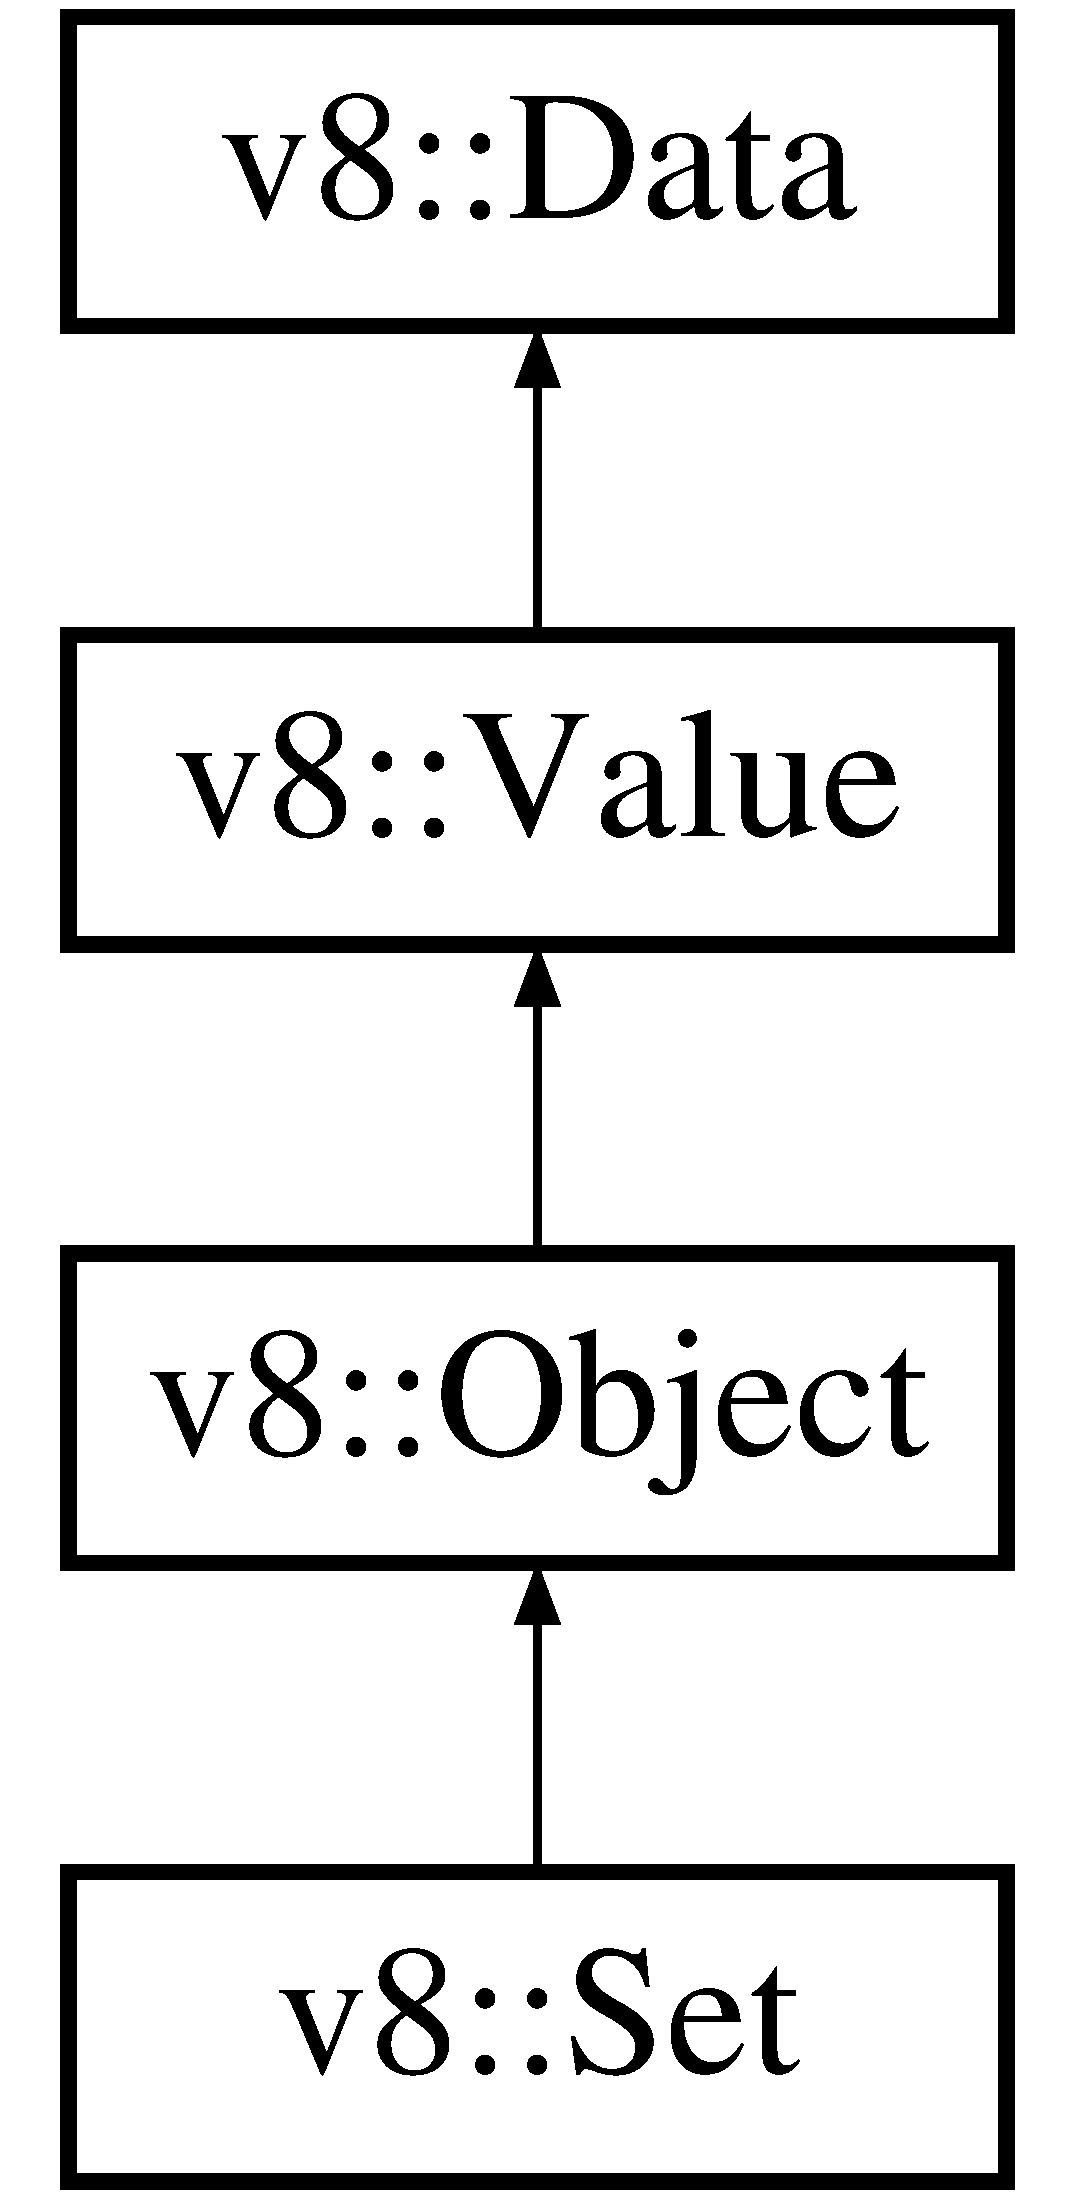
\includegraphics[height=4.000000cm]{classv8_1_1_set}
\end{center}
\end{figure}
\subsection*{Public Member Functions}
\begin{DoxyCompactItemize}
\item 
size\+\_\+t {\bfseries Size} () const \hypertarget{classv8_1_1_set_a7ae1a3522f51a8061813f562086baa91}{}\label{classv8_1_1_set_a7ae1a3522f51a8061813f562086baa91}

\item 
void {\bfseries Clear} ()\hypertarget{classv8_1_1_set_a5f7e4dbd6729a503ca617415d5eeedf0}{}\label{classv8_1_1_set_a5f7e4dbd6729a503ca617415d5eeedf0}

\item 
V8\+\_\+\+W\+A\+R\+N\+\_\+\+U\+N\+U\+S\+E\+D\+\_\+\+R\+E\+S\+U\+LT \hyperlink{classv8_1_1_maybe_local}{Maybe\+Local}$<$ \hyperlink{classv8_1_1_set}{Set} $>$ {\bfseries Add} (\hyperlink{classv8_1_1_local}{Local}$<$ \hyperlink{classv8_1_1_context}{Context} $>$ context, \hyperlink{classv8_1_1_local}{Local}$<$ \hyperlink{classv8_1_1_value}{Value} $>$ key)\hypertarget{classv8_1_1_set_adb56ad9dfa7541746b7894c359095801}{}\label{classv8_1_1_set_adb56ad9dfa7541746b7894c359095801}

\item 
V8\+\_\+\+W\+A\+R\+N\+\_\+\+U\+N\+U\+S\+E\+D\+\_\+\+R\+E\+S\+U\+LT \hyperlink{classv8_1_1_maybe}{Maybe}$<$ bool $>$ {\bfseries Has} (\hyperlink{classv8_1_1_local}{Local}$<$ \hyperlink{classv8_1_1_context}{Context} $>$ context, \hyperlink{classv8_1_1_local}{Local}$<$ \hyperlink{classv8_1_1_value}{Value} $>$ key)\hypertarget{classv8_1_1_set_a45a2c9e7b69d7bc7e94521d1ebfcce1d}{}\label{classv8_1_1_set_a45a2c9e7b69d7bc7e94521d1ebfcce1d}

\item 
V8\+\_\+\+W\+A\+R\+N\+\_\+\+U\+N\+U\+S\+E\+D\+\_\+\+R\+E\+S\+U\+LT \hyperlink{classv8_1_1_maybe}{Maybe}$<$ bool $>$ {\bfseries Delete} (\hyperlink{classv8_1_1_local}{Local}$<$ \hyperlink{classv8_1_1_context}{Context} $>$ context, \hyperlink{classv8_1_1_local}{Local}$<$ \hyperlink{classv8_1_1_value}{Value} $>$ key)\hypertarget{classv8_1_1_set_a638909072ad2de7fe0e207e4889ea9bf}{}\label{classv8_1_1_set_a638909072ad2de7fe0e207e4889ea9bf}

\item 
\hyperlink{classv8_1_1_local}{Local}$<$ \hyperlink{classv8_1_1_array}{Array} $>$ \hyperlink{classv8_1_1_set_a842e7012acb15f502f9a87d0c7c0b78d}{As\+Array} () const 
\end{DoxyCompactItemize}
\subsection*{Static Public Member Functions}
\begin{DoxyCompactItemize}
\item 
static \hyperlink{classv8_1_1_local}{Local}$<$ \hyperlink{classv8_1_1_set}{Set} $>$ \hyperlink{classv8_1_1_set_a036e773566a36997a79e78ef0a4103a1}{New} (\hyperlink{classv8_1_1_isolate}{Isolate} $\ast$isolate)
\item 
static V8\+\_\+\+I\+N\+L\+I\+NE \hyperlink{classv8_1_1_set}{Set} $\ast$ {\bfseries Cast} (\hyperlink{classv8_1_1_value}{Value} $\ast$obj)\hypertarget{classv8_1_1_set_a1739da4ee6bf39c381b83023f653e995}{}\label{classv8_1_1_set_a1739da4ee6bf39c381b83023f653e995}

\end{DoxyCompactItemize}
\subsection*{Static Private Member Functions}
\begin{DoxyCompactItemize}
\item 
static void {\bfseries Check\+Cast} (\hyperlink{classv8_1_1_value}{Value} $\ast$obj)\hypertarget{classv8_1_1_set_a64603aad9354099fb5ec0b19394e6678}{}\label{classv8_1_1_set_a64603aad9354099fb5ec0b19394e6678}

\end{DoxyCompactItemize}


\subsection{Detailed Description}
An instance of the built-\/in \hyperlink{classv8_1_1_set}{Set} constructor (E\+C\+M\+A-\/262, 6th Edition, 23.\+2.\+1). 

\subsection{Member Function Documentation}
\index{v8\+::\+Set@{v8\+::\+Set}!As\+Array@{As\+Array}}
\index{As\+Array@{As\+Array}!v8\+::\+Set@{v8\+::\+Set}}
\subsubsection[{\texorpdfstring{As\+Array() const }{AsArray() const }}]{\setlength{\rightskip}{0pt plus 5cm}{\bf Local}$<${\bf Array}$>$ v8\+::\+Set\+::\+As\+Array (
\begin{DoxyParamCaption}
{}
\end{DoxyParamCaption}
) const}\hypertarget{classv8_1_1_set_a842e7012acb15f502f9a87d0c7c0b78d}{}\label{classv8_1_1_set_a842e7012acb15f502f9a87d0c7c0b78d}
Returns an array of the keys in this \hyperlink{classv8_1_1_set}{Set}. \index{v8\+::\+Set@{v8\+::\+Set}!New@{New}}
\index{New@{New}!v8\+::\+Set@{v8\+::\+Set}}
\subsubsection[{\texorpdfstring{New(\+Isolate $\ast$isolate)}{New(Isolate *isolate)}}]{\setlength{\rightskip}{0pt plus 5cm}static {\bf Local}$<${\bf Set}$>$ v8\+::\+Set\+::\+New (
\begin{DoxyParamCaption}
\item[{{\bf Isolate} $\ast$}]{isolate}
\end{DoxyParamCaption}
)\hspace{0.3cm}{\ttfamily [static]}}\hypertarget{classv8_1_1_set_a036e773566a36997a79e78ef0a4103a1}{}\label{classv8_1_1_set_a036e773566a36997a79e78ef0a4103a1}
Creates a new empty \hyperlink{classv8_1_1_set}{Set}. 

The documentation for this class was generated from the following file\+:\begin{DoxyCompactItemize}
\item 
include/v8.\+h\end{DoxyCompactItemize}

\hypertarget{classv8_1_1_shared_array_buffer}{}\section{v8\+:\+:Shared\+Array\+Buffer Class Reference}
\label{classv8_1_1_shared_array_buffer}\index{v8\+::\+Shared\+Array\+Buffer@{v8\+::\+Shared\+Array\+Buffer}}


{\ttfamily \#include $<$v8.\+h$>$}

Inheritance diagram for v8\+:\+:Shared\+Array\+Buffer\+:\begin{figure}[H]
\begin{center}
\leavevmode
\includegraphics[height=4.000000cm]{classv8_1_1_shared_array_buffer}
\end{center}
\end{figure}
\subsection*{Classes}
\begin{DoxyCompactItemize}
\item 
class \hyperlink{classv8_1_1_shared_array_buffer_1_1_contents}{Contents}
\end{DoxyCompactItemize}
\subsection*{Public Member Functions}
\begin{DoxyCompactItemize}
\item 
size\+\_\+t \hyperlink{classv8_1_1_shared_array_buffer_a09cfb461e2f3f8e1fca53a4a2fbfd8df}{Byte\+Length} () const 
\item 
bool \hyperlink{classv8_1_1_shared_array_buffer_a37e7ba1ed5a1422af9928697ea6a960b}{Is\+External} () const 
\item 
\hyperlink{classv8_1_1_shared_array_buffer_1_1_contents}{Contents} \hyperlink{classv8_1_1_shared_array_buffer_a5e3308ea38c81c37d5c3fc08fc1a6696}{Externalize} ()
\item 
\hyperlink{classv8_1_1_shared_array_buffer_1_1_contents}{Contents} \hyperlink{classv8_1_1_shared_array_buffer_a7267c4156bea02154afa6c8fc5b1f4d8}{Get\+Contents} ()
\end{DoxyCompactItemize}
\subsection*{Static Public Member Functions}
\begin{DoxyCompactItemize}
\item 
static \hyperlink{classv8_1_1_local}{Local}$<$ \hyperlink{classv8_1_1_shared_array_buffer}{Shared\+Array\+Buffer} $>$ \hyperlink{classv8_1_1_shared_array_buffer_a3162c3d636c0c184db7001086f68a79a}{New} (\hyperlink{classv8_1_1_isolate}{Isolate} $\ast$isolate, size\+\_\+t byte\+\_\+length)
\item 
static \hyperlink{classv8_1_1_local}{Local}$<$ \hyperlink{classv8_1_1_shared_array_buffer}{Shared\+Array\+Buffer} $>$ \hyperlink{classv8_1_1_shared_array_buffer_ada351f205ccc0cb9616df676beda7d17}{New} (\hyperlink{classv8_1_1_isolate}{Isolate} $\ast$isolate, void $\ast$data, size\+\_\+t byte\+\_\+length, Array\+Buffer\+Creation\+Mode mode=Array\+Buffer\+Creation\+Mode\+::k\+Externalized)
\item 
static V8\+\_\+\+I\+N\+L\+I\+NE \hyperlink{classv8_1_1_shared_array_buffer}{Shared\+Array\+Buffer} $\ast$ {\bfseries Cast} (\hyperlink{classv8_1_1_value}{Value} $\ast$obj)\hypertarget{classv8_1_1_shared_array_buffer_ac4e1ba5d4564c7033814f4cc45fdda84}{}\label{classv8_1_1_shared_array_buffer_ac4e1ba5d4564c7033814f4cc45fdda84}

\end{DoxyCompactItemize}
\subsection*{Static Public Attributes}
\begin{DoxyCompactItemize}
\item 
static const int {\bfseries k\+Internal\+Field\+Count} = V8\+\_\+\+A\+R\+R\+A\+Y\+\_\+\+B\+U\+F\+F\+E\+R\+\_\+\+I\+N\+T\+E\+R\+N\+A\+L\+\_\+\+F\+I\+E\+L\+D\+\_\+\+C\+O\+U\+NT\hypertarget{classv8_1_1_shared_array_buffer_a6f47f6b441e37aefd1a9d0176e8a3da8}{}\label{classv8_1_1_shared_array_buffer_a6f47f6b441e37aefd1a9d0176e8a3da8}

\end{DoxyCompactItemize}
\subsection*{Static Private Member Functions}
\begin{DoxyCompactItemize}
\item 
static void {\bfseries Check\+Cast} (\hyperlink{classv8_1_1_value}{Value} $\ast$obj)\hypertarget{classv8_1_1_shared_array_buffer_a9cb59d11c38b3caaf11fa74436d8b34f}{}\label{classv8_1_1_shared_array_buffer_a9cb59d11c38b3caaf11fa74436d8b34f}

\end{DoxyCompactItemize}


\subsection{Detailed Description}
An instance of the built-\/in \hyperlink{classv8_1_1_shared_array_buffer}{Shared\+Array\+Buffer} constructor. This A\+PI is experimental and may change significantly. 

\subsection{Member Function Documentation}
\index{v8\+::\+Shared\+Array\+Buffer@{v8\+::\+Shared\+Array\+Buffer}!Byte\+Length@{Byte\+Length}}
\index{Byte\+Length@{Byte\+Length}!v8\+::\+Shared\+Array\+Buffer@{v8\+::\+Shared\+Array\+Buffer}}
\subsubsection[{\texorpdfstring{Byte\+Length() const }{ByteLength() const }}]{\setlength{\rightskip}{0pt plus 5cm}size\+\_\+t v8\+::\+Shared\+Array\+Buffer\+::\+Byte\+Length (
\begin{DoxyParamCaption}
{}
\end{DoxyParamCaption}
) const}\hypertarget{classv8_1_1_shared_array_buffer_a09cfb461e2f3f8e1fca53a4a2fbfd8df}{}\label{classv8_1_1_shared_array_buffer_a09cfb461e2f3f8e1fca53a4a2fbfd8df}
\hyperlink{classv8_1_1_data}{Data} length in bytes. \index{v8\+::\+Shared\+Array\+Buffer@{v8\+::\+Shared\+Array\+Buffer}!Externalize@{Externalize}}
\index{Externalize@{Externalize}!v8\+::\+Shared\+Array\+Buffer@{v8\+::\+Shared\+Array\+Buffer}}
\subsubsection[{\texorpdfstring{Externalize()}{Externalize()}}]{\setlength{\rightskip}{0pt plus 5cm}{\bf v8\+::\+Shared\+Array\+Buffer\+::\+Contents} v8\+::\+Shared\+Array\+Buffer\+::\+Externalize (
\begin{DoxyParamCaption}
{}
\end{DoxyParamCaption}
)}\hypertarget{classv8_1_1_shared_array_buffer_a5e3308ea38c81c37d5c3fc08fc1a6696}{}\label{classv8_1_1_shared_array_buffer_a5e3308ea38c81c37d5c3fc08fc1a6696}
Make this \hyperlink{classv8_1_1_shared_array_buffer}{Shared\+Array\+Buffer} external. The pointer to underlying memory block and byte length are returned as $\vert$\+Contents$\vert$ structure. After \hyperlink{classv8_1_1_shared_array_buffer}{Shared\+Array\+Buffer} had been etxrenalized, it does no longer owns the memory block. The caller should take steps to free memory when it is no longer needed.

The memory block is guaranteed to be allocated with $\vert$\+Allocator\+::\+Allocate$\vert$ by the allocator specified in \hyperlink{structv8_1_1_isolate_1_1_create_params_a7c663f70b64290392eeaf164f57585f9}{v8\+::\+Isolate\+::\+Create\+Params\+::array\+\_\+buffer\+\_\+allocator}. \index{v8\+::\+Shared\+Array\+Buffer@{v8\+::\+Shared\+Array\+Buffer}!Get\+Contents@{Get\+Contents}}
\index{Get\+Contents@{Get\+Contents}!v8\+::\+Shared\+Array\+Buffer@{v8\+::\+Shared\+Array\+Buffer}}
\subsubsection[{\texorpdfstring{Get\+Contents()}{GetContents()}}]{\setlength{\rightskip}{0pt plus 5cm}{\bf v8\+::\+Shared\+Array\+Buffer\+::\+Contents} v8\+::\+Shared\+Array\+Buffer\+::\+Get\+Contents (
\begin{DoxyParamCaption}
{}
\end{DoxyParamCaption}
)}\hypertarget{classv8_1_1_shared_array_buffer_a7267c4156bea02154afa6c8fc5b1f4d8}{}\label{classv8_1_1_shared_array_buffer_a7267c4156bea02154afa6c8fc5b1f4d8}
Get a pointer to the \hyperlink{classv8_1_1_array_buffer}{Array\+Buffer}\textquotesingle{}s underlying memory block without externalizing it. If the \hyperlink{classv8_1_1_array_buffer}{Array\+Buffer} is not externalized, this pointer will become invalid as soon as the \hyperlink{classv8_1_1_array_buffer}{Array\+Buffer} became garbage collected.

The embedder should make sure to hold a strong reference to the \hyperlink{classv8_1_1_array_buffer}{Array\+Buffer} while accessing this pointer.

The memory block is guaranteed to be allocated with $\vert$\+Allocator\+::\+Allocate$\vert$ by the allocator specified in \hyperlink{structv8_1_1_isolate_1_1_create_params_a7c663f70b64290392eeaf164f57585f9}{v8\+::\+Isolate\+::\+Create\+Params\+::array\+\_\+buffer\+\_\+allocator}. \index{v8\+::\+Shared\+Array\+Buffer@{v8\+::\+Shared\+Array\+Buffer}!Is\+External@{Is\+External}}
\index{Is\+External@{Is\+External}!v8\+::\+Shared\+Array\+Buffer@{v8\+::\+Shared\+Array\+Buffer}}
\subsubsection[{\texorpdfstring{Is\+External() const }{IsExternal() const }}]{\setlength{\rightskip}{0pt plus 5cm}bool v8\+::\+Shared\+Array\+Buffer\+::\+Is\+External (
\begin{DoxyParamCaption}
{}
\end{DoxyParamCaption}
) const}\hypertarget{classv8_1_1_shared_array_buffer_a37e7ba1ed5a1422af9928697ea6a960b}{}\label{classv8_1_1_shared_array_buffer_a37e7ba1ed5a1422af9928697ea6a960b}
Returns true if \hyperlink{classv8_1_1_shared_array_buffer}{Shared\+Array\+Buffer} is externalized, that is, does not own its memory block. \index{v8\+::\+Shared\+Array\+Buffer@{v8\+::\+Shared\+Array\+Buffer}!New@{New}}
\index{New@{New}!v8\+::\+Shared\+Array\+Buffer@{v8\+::\+Shared\+Array\+Buffer}}
\subsubsection[{\texorpdfstring{New(\+Isolate $\ast$isolate, size\+\_\+t byte\+\_\+length)}{New(Isolate *isolate, size_t byte_length)}}]{\setlength{\rightskip}{0pt plus 5cm}{\bf Local}$<$ {\bf Shared\+Array\+Buffer} $>$ v8\+::\+Shared\+Array\+Buffer\+::\+New (
\begin{DoxyParamCaption}
\item[{{\bf Isolate} $\ast$}]{isolate, }
\item[{size\+\_\+t}]{byte\+\_\+length}
\end{DoxyParamCaption}
)\hspace{0.3cm}{\ttfamily [static]}}\hypertarget{classv8_1_1_shared_array_buffer_a3162c3d636c0c184db7001086f68a79a}{}\label{classv8_1_1_shared_array_buffer_a3162c3d636c0c184db7001086f68a79a}
Create a new \hyperlink{classv8_1_1_shared_array_buffer}{Shared\+Array\+Buffer}. Allocate $\vert$byte\+\_\+length$\vert$ bytes. Allocated memory will be owned by a created \hyperlink{classv8_1_1_shared_array_buffer}{Shared\+Array\+Buffer} and will be deallocated when it is garbage-\/collected, unless the object is externalized. \index{v8\+::\+Shared\+Array\+Buffer@{v8\+::\+Shared\+Array\+Buffer}!New@{New}}
\index{New@{New}!v8\+::\+Shared\+Array\+Buffer@{v8\+::\+Shared\+Array\+Buffer}}
\subsubsection[{\texorpdfstring{New(\+Isolate $\ast$isolate, void $\ast$data, size\+\_\+t byte\+\_\+length, Array\+Buffer\+Creation\+Mode mode=\+Array\+Buffer\+Creation\+Mode\+::k\+Externalized)}{New(Isolate *isolate, void *data, size_t byte_length, ArrayBufferCreationMode mode=ArrayBufferCreationMode::kExternalized)}}]{\setlength{\rightskip}{0pt plus 5cm}{\bf Local}$<$ {\bf Shared\+Array\+Buffer} $>$ v8\+::\+Shared\+Array\+Buffer\+::\+New (
\begin{DoxyParamCaption}
\item[{{\bf Isolate} $\ast$}]{isolate, }
\item[{void $\ast$}]{data, }
\item[{size\+\_\+t}]{byte\+\_\+length, }
\item[{Array\+Buffer\+Creation\+Mode}]{mode = {\ttfamily ArrayBufferCreationMode\+:\+:kExternalized}}
\end{DoxyParamCaption}
)\hspace{0.3cm}{\ttfamily [static]}}\hypertarget{classv8_1_1_shared_array_buffer_ada351f205ccc0cb9616df676beda7d17}{}\label{classv8_1_1_shared_array_buffer_ada351f205ccc0cb9616df676beda7d17}
Create a new \hyperlink{classv8_1_1_shared_array_buffer}{Shared\+Array\+Buffer} over an existing memory block. The created array buffer is immediately in externalized state unless otherwise specified. The memory block will not be reclaimed when a created \hyperlink{classv8_1_1_shared_array_buffer}{Shared\+Array\+Buffer} is garbage-\/collected. 

The documentation for this class was generated from the following files\+:\begin{DoxyCompactItemize}
\item 
/\+Users/joshgav/node/v8/include/v8.\+h\item 
/\+Users/joshgav/node/v8/src/api.\+cc\end{DoxyCompactItemize}

\hypertarget{classv8_1_1_signature}{}\section{v8\+:\+:Signature Class Reference}
\label{classv8_1_1_signature}\index{v8\+::\+Signature@{v8\+::\+Signature}}


{\ttfamily \#include $<$v8.\+h$>$}

Inheritance diagram for v8\+:\+:Signature\+:\begin{figure}[H]
\begin{center}
\leavevmode
\includegraphics[height=2.000000cm]{classv8_1_1_signature}
\end{center}
\end{figure}
\subsection*{Static Public Member Functions}
\begin{DoxyCompactItemize}
\item 
static \hyperlink{classv8_1_1_local}{Local}$<$ \hyperlink{classv8_1_1_signature}{Signature} $>$ {\bfseries New} (\hyperlink{classv8_1_1_isolate}{Isolate} $\ast$isolate, \hyperlink{classv8_1_1_local}{Local}$<$ \hyperlink{classv8_1_1_function_template}{Function\+Template} $>$ receiver=\hyperlink{classv8_1_1_local}{Local}$<$ \hyperlink{classv8_1_1_function_template}{Function\+Template} $>$())\hypertarget{classv8_1_1_signature_a4e3d622674ec1f735e9981ec3309320f}{}\label{classv8_1_1_signature_a4e3d622674ec1f735e9981ec3309320f}

\end{DoxyCompactItemize}


\subsection{Detailed Description}
A \hyperlink{classv8_1_1_signature}{Signature} specifies which receiver is valid for a function. 

The documentation for this class was generated from the following file\+:\begin{DoxyCompactItemize}
\item 
/\+Users/joshgav/node/v8/include/v8.\+h\end{DoxyCompactItemize}

\hypertarget{structv8_1_1internal_1_1_smi_tagging}{}\section{v8\+:\+:internal\+:\+:Smi\+Tagging$<$ ptr\+\_\+size $>$ Struct Template Reference}
\label{structv8_1_1internal_1_1_smi_tagging}\index{v8\+::internal\+::\+Smi\+Tagging$<$ ptr\+\_\+size $>$@{v8\+::internal\+::\+Smi\+Tagging$<$ ptr\+\_\+size $>$}}


The documentation for this struct was generated from the following file\+:\begin{DoxyCompactItemize}
\item 
include/v8.\+h\end{DoxyCompactItemize}

\hypertarget{structv8_1_1internal_1_1_smi_tagging_3_014_01_4}{}\section{v8\+:\+:internal\+:\+:Smi\+Tagging$<$ 4 $>$ Struct Template Reference}
\label{structv8_1_1internal_1_1_smi_tagging_3_014_01_4}\index{v8\+::internal\+::\+Smi\+Tagging$<$ 4 $>$@{v8\+::internal\+::\+Smi\+Tagging$<$ 4 $>$}}
\subsection*{Public Types}
\begin{DoxyCompactItemize}
\item 
enum \{ \\*
{\bfseries k\+Smi\+Shift\+Size} = 0, 
\\*
{\bfseries k\+Smi\+Value\+Size} = 31
 \}\hypertarget{structv8_1_1internal_1_1_smi_tagging_3_014_01_4_a4a08a18726d053536f2e1988bb1e1cfa}{}\label{structv8_1_1internal_1_1_smi_tagging_3_014_01_4_a4a08a18726d053536f2e1988bb1e1cfa}

\end{DoxyCompactItemize}
\subsection*{Static Public Member Functions}
\begin{DoxyCompactItemize}
\item 
static int {\bfseries Smi\+Shift\+Size} ()\hypertarget{structv8_1_1internal_1_1_smi_tagging_3_014_01_4_a6b4e44bb5de76851c70fb604e1a7a019}{}\label{structv8_1_1internal_1_1_smi_tagging_3_014_01_4_a6b4e44bb5de76851c70fb604e1a7a019}

\item 
static int {\bfseries Smi\+Value\+Size} ()\hypertarget{structv8_1_1internal_1_1_smi_tagging_3_014_01_4_a07e9a8ef19de5cb4bba23cd9756d7b3e}{}\label{structv8_1_1internal_1_1_smi_tagging_3_014_01_4_a07e9a8ef19de5cb4bba23cd9756d7b3e}

\item 
static V8\+\_\+\+I\+N\+L\+I\+NE int {\bfseries Smi\+To\+Int} (const internal\+::\+Object $\ast$value)\hypertarget{structv8_1_1internal_1_1_smi_tagging_3_014_01_4_a62bf3521541e99483c8d0743685dc375}{}\label{structv8_1_1internal_1_1_smi_tagging_3_014_01_4_a62bf3521541e99483c8d0743685dc375}

\item 
static V8\+\_\+\+I\+N\+L\+I\+NE internal\+::\+Object $\ast$ {\bfseries Int\+To\+Smi} (int value)\hypertarget{structv8_1_1internal_1_1_smi_tagging_3_014_01_4_abbc2788d901a590f3b9276e7e0d4059b}{}\label{structv8_1_1internal_1_1_smi_tagging_3_014_01_4_abbc2788d901a590f3b9276e7e0d4059b}

\item 
static V8\+\_\+\+I\+N\+L\+I\+NE bool {\bfseries Is\+Valid\+Smi} (intptr\+\_\+t value)\hypertarget{structv8_1_1internal_1_1_smi_tagging_3_014_01_4_a7ca3b3a7b14e2fbea5decac3675ac619}{}\label{structv8_1_1internal_1_1_smi_tagging_3_014_01_4_a7ca3b3a7b14e2fbea5decac3675ac619}

\end{DoxyCompactItemize}


The documentation for this struct was generated from the following file\+:\begin{DoxyCompactItemize}
\item 
include/v8.\+h\end{DoxyCompactItemize}

\hypertarget{structv8_1_1internal_1_1_smi_tagging_3_018_01_4}{}\section{v8\+:\+:internal\+:\+:Smi\+Tagging$<$ 8 $>$ Struct Template Reference}
\label{structv8_1_1internal_1_1_smi_tagging_3_018_01_4}\index{v8\+::internal\+::\+Smi\+Tagging$<$ 8 $>$@{v8\+::internal\+::\+Smi\+Tagging$<$ 8 $>$}}
\subsection*{Public Types}
\begin{DoxyCompactItemize}
\item 
enum \{ \\*
{\bfseries k\+Smi\+Shift\+Size} = 31, 
\\*
{\bfseries k\+Smi\+Value\+Size} = 32
 \}\hypertarget{structv8_1_1internal_1_1_smi_tagging_3_018_01_4_aca1e57809e36a53b790ee0480324fb7b}{}\label{structv8_1_1internal_1_1_smi_tagging_3_018_01_4_aca1e57809e36a53b790ee0480324fb7b}

\end{DoxyCompactItemize}
\subsection*{Static Public Member Functions}
\begin{DoxyCompactItemize}
\item 
static int {\bfseries Smi\+Shift\+Size} ()\hypertarget{structv8_1_1internal_1_1_smi_tagging_3_018_01_4_a4fb28f586fdee8316a03f9b8f94b945d}{}\label{structv8_1_1internal_1_1_smi_tagging_3_018_01_4_a4fb28f586fdee8316a03f9b8f94b945d}

\item 
static int {\bfseries Smi\+Value\+Size} ()\hypertarget{structv8_1_1internal_1_1_smi_tagging_3_018_01_4_a836e783af92beb7ca9cc8cdabef43ab2}{}\label{structv8_1_1internal_1_1_smi_tagging_3_018_01_4_a836e783af92beb7ca9cc8cdabef43ab2}

\item 
static V8\+\_\+\+I\+N\+L\+I\+NE int {\bfseries Smi\+To\+Int} (const internal\+::\+Object $\ast$value)\hypertarget{structv8_1_1internal_1_1_smi_tagging_3_018_01_4_a040db1ceee3195c2463075b7b50cfda0}{}\label{structv8_1_1internal_1_1_smi_tagging_3_018_01_4_a040db1ceee3195c2463075b7b50cfda0}

\item 
static V8\+\_\+\+I\+N\+L\+I\+NE internal\+::\+Object $\ast$ {\bfseries Int\+To\+Smi} (int value)\hypertarget{structv8_1_1internal_1_1_smi_tagging_3_018_01_4_a1926f38e35fc98fe244e8136180d70f2}{}\label{structv8_1_1internal_1_1_smi_tagging_3_018_01_4_a1926f38e35fc98fe244e8136180d70f2}

\item 
static V8\+\_\+\+I\+N\+L\+I\+NE bool {\bfseries Is\+Valid\+Smi} (intptr\+\_\+t value)\hypertarget{structv8_1_1internal_1_1_smi_tagging_3_018_01_4_a5ab93d4cf7c3b9ceff5116b3598a1f94}{}\label{structv8_1_1internal_1_1_smi_tagging_3_018_01_4_a5ab93d4cf7c3b9ceff5116b3598a1f94}

\end{DoxyCompactItemize}


The documentation for this struct was generated from the following file\+:\begin{DoxyCompactItemize}
\item 
include/v8.\+h\end{DoxyCompactItemize}

\hypertarget{classv8_1_1_script_compiler_1_1_source}{}\section{v8\+:\+:Script\+Compiler\+:\+:Source Class Reference}
\label{classv8_1_1_script_compiler_1_1_source}\index{v8\+::\+Script\+Compiler\+::\+Source@{v8\+::\+Script\+Compiler\+::\+Source}}


{\ttfamily \#include $<$v8.\+h$>$}

\subsection*{Public Member Functions}
\begin{DoxyCompactItemize}
\item 
V8\+\_\+\+I\+N\+L\+I\+NE {\bfseries Source} (\hyperlink{classv8_1_1_local}{Local}$<$ \hyperlink{classv8_1_1_string}{String} $>$ source\+\_\+string, const \hyperlink{classv8_1_1_script_origin}{Script\+Origin} \&origin, \hyperlink{structv8_1_1_script_compiler_1_1_cached_data}{Cached\+Data} $\ast$cached\+\_\+data=N\+U\+LL)\hypertarget{classv8_1_1_script_compiler_1_1_source_ae71a5fe18124d71f9acfcc872310d586}{}\label{classv8_1_1_script_compiler_1_1_source_ae71a5fe18124d71f9acfcc872310d586}

\item 
V8\+\_\+\+I\+N\+L\+I\+NE {\bfseries Source} (\hyperlink{classv8_1_1_local}{Local}$<$ \hyperlink{classv8_1_1_string}{String} $>$ source\+\_\+string, \hyperlink{structv8_1_1_script_compiler_1_1_cached_data}{Cached\+Data} $\ast$cached\+\_\+data=N\+U\+LL)\hypertarget{classv8_1_1_script_compiler_1_1_source_ad46e9d298cf3199c3a570182a680449d}{}\label{classv8_1_1_script_compiler_1_1_source_ad46e9d298cf3199c3a570182a680449d}

\item 
V8\+\_\+\+I\+N\+L\+I\+NE const \hyperlink{structv8_1_1_script_compiler_1_1_cached_data}{Cached\+Data} $\ast$ {\bfseries Get\+Cached\+Data} () const \hypertarget{classv8_1_1_script_compiler_1_1_source_a7cef3113a46627fefa3110132acf47d2}{}\label{classv8_1_1_script_compiler_1_1_source_a7cef3113a46627fefa3110132acf47d2}

\end{DoxyCompactItemize}
\subsection*{Private Member Functions}
\begin{DoxyCompactItemize}
\item 
{\bfseries Source} (const \hyperlink{classv8_1_1_script_compiler_1_1_source}{Source} \&)\hypertarget{classv8_1_1_script_compiler_1_1_source_ac4d4f4ab70c2daf63d69c59fe0a6f94a}{}\label{classv8_1_1_script_compiler_1_1_source_ac4d4f4ab70c2daf63d69c59fe0a6f94a}

\item 
\hyperlink{classv8_1_1_script_compiler_1_1_source}{Source} \& {\bfseries operator=} (const \hyperlink{classv8_1_1_script_compiler_1_1_source}{Source} \&)\hypertarget{classv8_1_1_script_compiler_1_1_source_af539e88c6c7f06d31ea7fba8013fc09e}{}\label{classv8_1_1_script_compiler_1_1_source_af539e88c6c7f06d31ea7fba8013fc09e}

\end{DoxyCompactItemize}
\subsection*{Private Attributes}
\begin{DoxyCompactItemize}
\item 
\hyperlink{classv8_1_1_local}{Local}$<$ \hyperlink{classv8_1_1_string}{String} $>$ {\bfseries source\+\_\+string}\hypertarget{classv8_1_1_script_compiler_1_1_source_a07fc4acec0a44fe51d2c01ec2b5dce17}{}\label{classv8_1_1_script_compiler_1_1_source_a07fc4acec0a44fe51d2c01ec2b5dce17}

\item 
\hyperlink{classv8_1_1_local}{Local}$<$ \hyperlink{classv8_1_1_value}{Value} $>$ {\bfseries resource\+\_\+name}\hypertarget{classv8_1_1_script_compiler_1_1_source_ace326950bf30503d42fee645dcdc2273}{}\label{classv8_1_1_script_compiler_1_1_source_ace326950bf30503d42fee645dcdc2273}

\item 
\hyperlink{classv8_1_1_local}{Local}$<$ \hyperlink{classv8_1_1_integer}{Integer} $>$ {\bfseries resource\+\_\+line\+\_\+offset}\hypertarget{classv8_1_1_script_compiler_1_1_source_ae05808989407c22b874a221ce6e90f36}{}\label{classv8_1_1_script_compiler_1_1_source_ae05808989407c22b874a221ce6e90f36}

\item 
\hyperlink{classv8_1_1_local}{Local}$<$ \hyperlink{classv8_1_1_integer}{Integer} $>$ {\bfseries resource\+\_\+column\+\_\+offset}\hypertarget{classv8_1_1_script_compiler_1_1_source_a1c2db9d7983e3168e855128520b1b086}{}\label{classv8_1_1_script_compiler_1_1_source_a1c2db9d7983e3168e855128520b1b086}

\item 
\hyperlink{classv8_1_1_script_origin_options}{Script\+Origin\+Options} {\bfseries resource\+\_\+options}\hypertarget{classv8_1_1_script_compiler_1_1_source_a6d56b93597b8f30c5f57a8c9ee423668}{}\label{classv8_1_1_script_compiler_1_1_source_a6d56b93597b8f30c5f57a8c9ee423668}

\item 
\hyperlink{classv8_1_1_local}{Local}$<$ \hyperlink{classv8_1_1_value}{Value} $>$ {\bfseries source\+\_\+map\+\_\+url}\hypertarget{classv8_1_1_script_compiler_1_1_source_aee5bd78af66487af33b2056dd059b906}{}\label{classv8_1_1_script_compiler_1_1_source_aee5bd78af66487af33b2056dd059b906}

\item 
\hyperlink{structv8_1_1_script_compiler_1_1_cached_data}{Cached\+Data} $\ast$ {\bfseries cached\+\_\+data}\hypertarget{classv8_1_1_script_compiler_1_1_source_a18de27fb68bf42b44fe981aa594c794d}{}\label{classv8_1_1_script_compiler_1_1_source_a18de27fb68bf42b44fe981aa594c794d}

\end{DoxyCompactItemize}
\subsection*{Friends}
\begin{DoxyCompactItemize}
\item 
class {\bfseries Script\+Compiler}\hypertarget{classv8_1_1_script_compiler_1_1_source_a1cb50af99960b4c11eaee7347e034f51}{}\label{classv8_1_1_script_compiler_1_1_source_a1cb50af99960b4c11eaee7347e034f51}

\end{DoxyCompactItemize}


\subsection{Detailed Description}
\hyperlink{classv8_1_1_script_compiler_1_1_source}{Source} code which can be then compiled to a \hyperlink{classv8_1_1_unbound_script}{Unbound\+Script} or \hyperlink{classv8_1_1_script}{Script}. 

The documentation for this class was generated from the following file\+:\begin{DoxyCompactItemize}
\item 
/\+Users/joshgav/node/v8/include/v8.\+h\end{DoxyCompactItemize}

\hypertarget{classv8_1_1_stack_frame}{}\section{v8\+:\+:Stack\+Frame Class Reference}
\label{classv8_1_1_stack_frame}\index{v8\+::\+Stack\+Frame@{v8\+::\+Stack\+Frame}}


{\ttfamily \#include $<$v8.\+h$>$}

\subsection*{Public Member Functions}
\begin{DoxyCompactItemize}
\item 
int \hyperlink{classv8_1_1_stack_frame_a57886e590ac1a4c57ee6f6bf1009b5b1}{Get\+Line\+Number} () const 
\item 
int \hyperlink{classv8_1_1_stack_frame_a44eccfb1bf17221ab6f69e977f3aa3a2}{Get\+Column} () const 
\item 
int \hyperlink{classv8_1_1_stack_frame_ac449d55656f8b7638de3cf5f5530cb7a}{Get\+Script\+Id} () const 
\item 
\hyperlink{classv8_1_1_local}{Local}$<$ \hyperlink{classv8_1_1_string}{String} $>$ \hyperlink{classv8_1_1_stack_frame_ac9701a5687dd04bcf24fd02f62bbe1a8}{Get\+Script\+Name} () const 
\item 
\hyperlink{classv8_1_1_local}{Local}$<$ \hyperlink{classv8_1_1_string}{String} $>$ \hyperlink{classv8_1_1_stack_frame_ac9f436f4cb245d871fe7efce03edc0cc}{Get\+Script\+Name\+Or\+Source\+U\+RL} () const 
\item 
\hyperlink{classv8_1_1_local}{Local}$<$ \hyperlink{classv8_1_1_string}{String} $>$ \hyperlink{classv8_1_1_stack_frame_ac13cdea4b4253d82485e673de6264073}{Get\+Function\+Name} () const 
\item 
bool \hyperlink{classv8_1_1_stack_frame_ae45f4d6ff9398a00a0b6534c160ec0c7}{Is\+Eval} () const 
\item 
bool \hyperlink{classv8_1_1_stack_frame_ade01313f4a3f6b88691d9d544737f65c}{Is\+Constructor} () const 
\end{DoxyCompactItemize}


\subsection{Detailed Description}
A single Java\+Script stack frame. 

\subsection{Member Function Documentation}
\index{v8\+::\+Stack\+Frame@{v8\+::\+Stack\+Frame}!Get\+Column@{Get\+Column}}
\index{Get\+Column@{Get\+Column}!v8\+::\+Stack\+Frame@{v8\+::\+Stack\+Frame}}
\subsubsection[{\texorpdfstring{Get\+Column() const }{GetColumn() const }}]{\setlength{\rightskip}{0pt plus 5cm}int v8\+::\+Stack\+Frame\+::\+Get\+Column (
\begin{DoxyParamCaption}
{}
\end{DoxyParamCaption}
) const}\hypertarget{classv8_1_1_stack_frame_a44eccfb1bf17221ab6f69e977f3aa3a2}{}\label{classv8_1_1_stack_frame_a44eccfb1bf17221ab6f69e977f3aa3a2}
Returns the 1-\/based column offset on the line for the associated function call. This method will return Message\+::k\+No\+Column\+Info if it is unable to retrieve the column number, or if k\+Column\+Offset was not passed as an option when capturing the \hyperlink{classv8_1_1_stack_trace}{Stack\+Trace}. \index{v8\+::\+Stack\+Frame@{v8\+::\+Stack\+Frame}!Get\+Function\+Name@{Get\+Function\+Name}}
\index{Get\+Function\+Name@{Get\+Function\+Name}!v8\+::\+Stack\+Frame@{v8\+::\+Stack\+Frame}}
\subsubsection[{\texorpdfstring{Get\+Function\+Name() const }{GetFunctionName() const }}]{\setlength{\rightskip}{0pt plus 5cm}{\bf Local}$<${\bf String}$>$ v8\+::\+Stack\+Frame\+::\+Get\+Function\+Name (
\begin{DoxyParamCaption}
{}
\end{DoxyParamCaption}
) const}\hypertarget{classv8_1_1_stack_frame_ac13cdea4b4253d82485e673de6264073}{}\label{classv8_1_1_stack_frame_ac13cdea4b4253d82485e673de6264073}
Returns the name of the function associated with this stack frame. \index{v8\+::\+Stack\+Frame@{v8\+::\+Stack\+Frame}!Get\+Line\+Number@{Get\+Line\+Number}}
\index{Get\+Line\+Number@{Get\+Line\+Number}!v8\+::\+Stack\+Frame@{v8\+::\+Stack\+Frame}}
\subsubsection[{\texorpdfstring{Get\+Line\+Number() const }{GetLineNumber() const }}]{\setlength{\rightskip}{0pt plus 5cm}int v8\+::\+Stack\+Frame\+::\+Get\+Line\+Number (
\begin{DoxyParamCaption}
{}
\end{DoxyParamCaption}
) const}\hypertarget{classv8_1_1_stack_frame_a57886e590ac1a4c57ee6f6bf1009b5b1}{}\label{classv8_1_1_stack_frame_a57886e590ac1a4c57ee6f6bf1009b5b1}
Returns the number, 1-\/based, of the line for the associate function call. This method will return Message\+::k\+No\+Line\+Number\+Info if it is unable to retrieve the line number, or if k\+Line\+Number was not passed as an option when capturing the \hyperlink{classv8_1_1_stack_trace}{Stack\+Trace}. \index{v8\+::\+Stack\+Frame@{v8\+::\+Stack\+Frame}!Get\+Script\+Id@{Get\+Script\+Id}}
\index{Get\+Script\+Id@{Get\+Script\+Id}!v8\+::\+Stack\+Frame@{v8\+::\+Stack\+Frame}}
\subsubsection[{\texorpdfstring{Get\+Script\+Id() const }{GetScriptId() const }}]{\setlength{\rightskip}{0pt plus 5cm}int v8\+::\+Stack\+Frame\+::\+Get\+Script\+Id (
\begin{DoxyParamCaption}
{}
\end{DoxyParamCaption}
) const}\hypertarget{classv8_1_1_stack_frame_ac449d55656f8b7638de3cf5f5530cb7a}{}\label{classv8_1_1_stack_frame_ac449d55656f8b7638de3cf5f5530cb7a}
Returns the id of the script for the function for this \hyperlink{classv8_1_1_stack_frame}{Stack\+Frame}. This method will return Message\+::k\+No\+Script\+Id\+Info if it is unable to retrieve the script id, or if k\+Script\+Id was not passed as an option when capturing the \hyperlink{classv8_1_1_stack_trace}{Stack\+Trace}. \index{v8\+::\+Stack\+Frame@{v8\+::\+Stack\+Frame}!Get\+Script\+Name@{Get\+Script\+Name}}
\index{Get\+Script\+Name@{Get\+Script\+Name}!v8\+::\+Stack\+Frame@{v8\+::\+Stack\+Frame}}
\subsubsection[{\texorpdfstring{Get\+Script\+Name() const }{GetScriptName() const }}]{\setlength{\rightskip}{0pt plus 5cm}{\bf Local}$<${\bf String}$>$ v8\+::\+Stack\+Frame\+::\+Get\+Script\+Name (
\begin{DoxyParamCaption}
{}
\end{DoxyParamCaption}
) const}\hypertarget{classv8_1_1_stack_frame_ac9701a5687dd04bcf24fd02f62bbe1a8}{}\label{classv8_1_1_stack_frame_ac9701a5687dd04bcf24fd02f62bbe1a8}
Returns the name of the resource that contains the script for the function for this \hyperlink{classv8_1_1_stack_frame}{Stack\+Frame}. \index{v8\+::\+Stack\+Frame@{v8\+::\+Stack\+Frame}!Get\+Script\+Name\+Or\+Source\+U\+RL@{Get\+Script\+Name\+Or\+Source\+U\+RL}}
\index{Get\+Script\+Name\+Or\+Source\+U\+RL@{Get\+Script\+Name\+Or\+Source\+U\+RL}!v8\+::\+Stack\+Frame@{v8\+::\+Stack\+Frame}}
\subsubsection[{\texorpdfstring{Get\+Script\+Name\+Or\+Source\+U\+R\+L() const }{GetScriptNameOrSourceURL() const }}]{\setlength{\rightskip}{0pt plus 5cm}{\bf Local}$<${\bf String}$>$ v8\+::\+Stack\+Frame\+::\+Get\+Script\+Name\+Or\+Source\+U\+RL (
\begin{DoxyParamCaption}
{}
\end{DoxyParamCaption}
) const}\hypertarget{classv8_1_1_stack_frame_ac9f436f4cb245d871fe7efce03edc0cc}{}\label{classv8_1_1_stack_frame_ac9f436f4cb245d871fe7efce03edc0cc}
Returns the name of the resource that contains the script for the function for this \hyperlink{classv8_1_1_stack_frame}{Stack\+Frame} or source\+U\+RL value if the script name is undefined and its source ends with //\# source\+U\+RL=... string or deprecated //@ source\+U\+RL=... string. \index{v8\+::\+Stack\+Frame@{v8\+::\+Stack\+Frame}!Is\+Constructor@{Is\+Constructor}}
\index{Is\+Constructor@{Is\+Constructor}!v8\+::\+Stack\+Frame@{v8\+::\+Stack\+Frame}}
\subsubsection[{\texorpdfstring{Is\+Constructor() const }{IsConstructor() const }}]{\setlength{\rightskip}{0pt plus 5cm}bool v8\+::\+Stack\+Frame\+::\+Is\+Constructor (
\begin{DoxyParamCaption}
{}
\end{DoxyParamCaption}
) const}\hypertarget{classv8_1_1_stack_frame_ade01313f4a3f6b88691d9d544737f65c}{}\label{classv8_1_1_stack_frame_ade01313f4a3f6b88691d9d544737f65c}
Returns whether or not the associated function is called as a constructor via \char`\"{}new\char`\"{}. \index{v8\+::\+Stack\+Frame@{v8\+::\+Stack\+Frame}!Is\+Eval@{Is\+Eval}}
\index{Is\+Eval@{Is\+Eval}!v8\+::\+Stack\+Frame@{v8\+::\+Stack\+Frame}}
\subsubsection[{\texorpdfstring{Is\+Eval() const }{IsEval() const }}]{\setlength{\rightskip}{0pt plus 5cm}bool v8\+::\+Stack\+Frame\+::\+Is\+Eval (
\begin{DoxyParamCaption}
{}
\end{DoxyParamCaption}
) const}\hypertarget{classv8_1_1_stack_frame_ae45f4d6ff9398a00a0b6534c160ec0c7}{}\label{classv8_1_1_stack_frame_ae45f4d6ff9398a00a0b6534c160ec0c7}
Returns whether or not the associated function is compiled via a call to eval(). 

The documentation for this class was generated from the following file\+:\begin{DoxyCompactItemize}
\item 
/\+Users/joshgav/node/v8/include/v8.\+h\end{DoxyCompactItemize}

\hypertarget{classv8_1_1_stack_trace}{}\section{v8\+:\+:Stack\+Trace Class Reference}
\label{classv8_1_1_stack_trace}\index{v8\+::\+Stack\+Trace@{v8\+::\+Stack\+Trace}}


{\ttfamily \#include $<$v8.\+h$>$}

\subsection*{Public Types}
\begin{DoxyCompactItemize}
\item 
enum \hyperlink{classv8_1_1_stack_trace_a9704e4a37949eb8eb8ccddbddf161492}{Stack\+Trace\+Options} \{ \\*
{\bfseries k\+Line\+Number} = 1, 
\\*
{\bfseries k\+Column\+Offset} = 1 $<$$<$ 1 $\vert$ k\+Line\+Number, 
\\*
{\bfseries k\+Script\+Name} = 1 $<$$<$ 2, 
\\*
{\bfseries k\+Function\+Name} = 1 $<$$<$ 3, 
\\*
{\bfseries k\+Is\+Eval} = 1 $<$$<$ 4, 
\\*
{\bfseries k\+Is\+Constructor} = 1 $<$$<$ 5, 
\\*
{\bfseries k\+Script\+Name\+Or\+Source\+U\+RL} = 1 $<$$<$ 6, 
\\*
{\bfseries k\+Script\+Id} = 1 $<$$<$ 7, 
\\*
{\bfseries k\+Expose\+Frames\+Across\+Security\+Origins} = 1 $<$$<$ 8, 
\\*
{\bfseries k\+Overview} = k\+Line\+Number $\vert$ k\+Column\+Offset $\vert$ k\+Script\+Name $\vert$ k\+Function\+Name, 
\\*
{\bfseries k\+Detailed} = k\+Overview $\vert$ k\+Is\+Eval $\vert$ k\+Is\+Constructor $\vert$ k\+Script\+Name\+Or\+Source\+U\+RL
 \}
\end{DoxyCompactItemize}
\subsection*{Public Member Functions}
\begin{DoxyCompactItemize}
\item 
\hyperlink{classv8_1_1_local}{Local}$<$ \hyperlink{classv8_1_1_stack_frame}{Stack\+Frame} $>$ \hyperlink{classv8_1_1_stack_trace_a6fd5ba809b5d87032d70d32f0b1a80e8}{Get\+Frame} (uint32\+\_\+t index) const 
\item 
int \hyperlink{classv8_1_1_stack_trace_aafafebce6c034f1f6f4a870e8f52431e}{Get\+Frame\+Count} () const 
\item 
\hyperlink{classv8_1_1_local}{Local}$<$ \hyperlink{classv8_1_1_array}{Array} $>$ \hyperlink{classv8_1_1_stack_trace_abd36f712b3ab986b572aa259b06bf5bd}{As\+Array} ()
\end{DoxyCompactItemize}
\subsection*{Static Public Member Functions}
\begin{DoxyCompactItemize}
\item 
static \hyperlink{classv8_1_1_local}{Local}$<$ \hyperlink{classv8_1_1_stack_trace}{Stack\+Trace} $>$ \hyperlink{classv8_1_1_stack_trace_a030e8de1b13d720bb2bfac5cb8bc914b}{Current\+Stack\+Trace} (\hyperlink{classv8_1_1_isolate}{Isolate} $\ast$isolate, int frame\+\_\+limit, \hyperlink{classv8_1_1_stack_trace_a9704e4a37949eb8eb8ccddbddf161492}{Stack\+Trace\+Options} options=k\+Overview)
\end{DoxyCompactItemize}


\subsection{Detailed Description}
Representation of a Java\+Script stack trace. The information collected is a snapshot of the execution stack and the information remains valid after execution continues. 

\subsection{Member Enumeration Documentation}
\index{v8\+::\+Stack\+Trace@{v8\+::\+Stack\+Trace}!Stack\+Trace\+Options@{Stack\+Trace\+Options}}
\index{Stack\+Trace\+Options@{Stack\+Trace\+Options}!v8\+::\+Stack\+Trace@{v8\+::\+Stack\+Trace}}
\subsubsection[{\texorpdfstring{Stack\+Trace\+Options}{StackTraceOptions}}]{\setlength{\rightskip}{0pt plus 5cm}enum {\bf v8\+::\+Stack\+Trace\+::\+Stack\+Trace\+Options}}\hypertarget{classv8_1_1_stack_trace_a9704e4a37949eb8eb8ccddbddf161492}{}\label{classv8_1_1_stack_trace_a9704e4a37949eb8eb8ccddbddf161492}
Flags that determine what information is placed captured for each \hyperlink{classv8_1_1_stack_frame}{Stack\+Frame} when grabbing the current stack trace. 

\subsection{Member Function Documentation}
\index{v8\+::\+Stack\+Trace@{v8\+::\+Stack\+Trace}!As\+Array@{As\+Array}}
\index{As\+Array@{As\+Array}!v8\+::\+Stack\+Trace@{v8\+::\+Stack\+Trace}}
\subsubsection[{\texorpdfstring{As\+Array()}{AsArray()}}]{\setlength{\rightskip}{0pt plus 5cm}{\bf Local}$<${\bf Array}$>$ v8\+::\+Stack\+Trace\+::\+As\+Array (
\begin{DoxyParamCaption}
{}
\end{DoxyParamCaption}
)}\hypertarget{classv8_1_1_stack_trace_abd36f712b3ab986b572aa259b06bf5bd}{}\label{classv8_1_1_stack_trace_abd36f712b3ab986b572aa259b06bf5bd}
Returns \hyperlink{classv8_1_1_stack_trace}{Stack\+Trace} as a \hyperlink{classv8_1_1_array}{v8\+::\+Array} that contains \hyperlink{classv8_1_1_stack_frame}{Stack\+Frame} objects. \index{v8\+::\+Stack\+Trace@{v8\+::\+Stack\+Trace}!Current\+Stack\+Trace@{Current\+Stack\+Trace}}
\index{Current\+Stack\+Trace@{Current\+Stack\+Trace}!v8\+::\+Stack\+Trace@{v8\+::\+Stack\+Trace}}
\subsubsection[{\texorpdfstring{Current\+Stack\+Trace(\+Isolate $\ast$isolate, int frame\+\_\+limit, Stack\+Trace\+Options options=k\+Overview)}{CurrentStackTrace(Isolate *isolate, int frame_limit, StackTraceOptions options=kOverview)}}]{\setlength{\rightskip}{0pt plus 5cm}static {\bf Local}$<${\bf Stack\+Trace}$>$ v8\+::\+Stack\+Trace\+::\+Current\+Stack\+Trace (
\begin{DoxyParamCaption}
\item[{{\bf Isolate} $\ast$}]{isolate, }
\item[{int}]{frame\+\_\+limit, }
\item[{{\bf Stack\+Trace\+Options}}]{options = {\ttfamily kOverview}}
\end{DoxyParamCaption}
)\hspace{0.3cm}{\ttfamily [static]}}\hypertarget{classv8_1_1_stack_trace_a030e8de1b13d720bb2bfac5cb8bc914b}{}\label{classv8_1_1_stack_trace_a030e8de1b13d720bb2bfac5cb8bc914b}
Grab a snapshot of the current Java\+Script execution stack.


\begin{DoxyParams}{Parameters}
{\em frame\+\_\+limit} & The maximum number of stack frames we want to capture. \\
\hline
{\em options} & Enumerates the set of things we will capture for each \hyperlink{classv8_1_1_stack_frame}{Stack\+Frame}. \\
\hline
\end{DoxyParams}
\index{v8\+::\+Stack\+Trace@{v8\+::\+Stack\+Trace}!Get\+Frame@{Get\+Frame}}
\index{Get\+Frame@{Get\+Frame}!v8\+::\+Stack\+Trace@{v8\+::\+Stack\+Trace}}
\subsubsection[{\texorpdfstring{Get\+Frame(uint32\+\_\+t index) const }{GetFrame(uint32_t index) const }}]{\setlength{\rightskip}{0pt plus 5cm}{\bf Local}$<${\bf Stack\+Frame}$>$ v8\+::\+Stack\+Trace\+::\+Get\+Frame (
\begin{DoxyParamCaption}
\item[{uint32\+\_\+t}]{index}
\end{DoxyParamCaption}
) const}\hypertarget{classv8_1_1_stack_trace_a6fd5ba809b5d87032d70d32f0b1a80e8}{}\label{classv8_1_1_stack_trace_a6fd5ba809b5d87032d70d32f0b1a80e8}
Returns a \hyperlink{classv8_1_1_stack_frame}{Stack\+Frame} at a particular index. \index{v8\+::\+Stack\+Trace@{v8\+::\+Stack\+Trace}!Get\+Frame\+Count@{Get\+Frame\+Count}}
\index{Get\+Frame\+Count@{Get\+Frame\+Count}!v8\+::\+Stack\+Trace@{v8\+::\+Stack\+Trace}}
\subsubsection[{\texorpdfstring{Get\+Frame\+Count() const }{GetFrameCount() const }}]{\setlength{\rightskip}{0pt plus 5cm}int v8\+::\+Stack\+Trace\+::\+Get\+Frame\+Count (
\begin{DoxyParamCaption}
{}
\end{DoxyParamCaption}
) const}\hypertarget{classv8_1_1_stack_trace_aafafebce6c034f1f6f4a870e8f52431e}{}\label{classv8_1_1_stack_trace_aafafebce6c034f1f6f4a870e8f52431e}
Returns the number of Stack\+Frames. 

The documentation for this class was generated from the following file\+:\begin{DoxyCompactItemize}
\item 
/\+Users/joshgav/node/v8/include/v8.\+h\end{DoxyCompactItemize}

\hypertarget{classv8_1_1_startup_data}{}\section{v8\+:\+:Startup\+Data Class Reference}
\label{classv8_1_1_startup_data}\index{v8\+::\+Startup\+Data@{v8\+::\+Startup\+Data}}
\subsection*{Public Attributes}
\begin{DoxyCompactItemize}
\item 
const char $\ast$ {\bfseries data}\hypertarget{classv8_1_1_startup_data_a8daf0c5282d7c465988757dc4ecda1af}{}\label{classv8_1_1_startup_data_a8daf0c5282d7c465988757dc4ecda1af}

\item 
int {\bfseries raw\+\_\+size}\hypertarget{classv8_1_1_startup_data_a2f797e167b2bebd18ddca83dedda6ffa}{}\label{classv8_1_1_startup_data_a2f797e167b2bebd18ddca83dedda6ffa}

\end{DoxyCompactItemize}


The documentation for this class was generated from the following file\+:\begin{DoxyCompactItemize}
\item 
include/v8.\+h\end{DoxyCompactItemize}

\hypertarget{classv8_1_1_std_global_value_map}{}\section{v8\+:\+:Std\+Global\+Value\+Map$<$ K, V, Traits $>$ Class Template Reference}
\label{classv8_1_1_std_global_value_map}\index{v8\+::\+Std\+Global\+Value\+Map$<$ K, V, Traits $>$@{v8\+::\+Std\+Global\+Value\+Map$<$ K, V, Traits $>$}}


{\ttfamily \#include $<$v8-\/util.\+h$>$}

Inheritance diagram for v8\+:\+:Std\+Global\+Value\+Map$<$ K, V, Traits $>$\+:\begin{figure}[H]
\begin{center}
\leavevmode
\includegraphics[height=3.000000cm]{classv8_1_1_std_global_value_map}
\end{center}
\end{figure}
\subsection*{Public Member Functions}
\begin{DoxyCompactItemize}
\item 
{\bfseries Std\+Global\+Value\+Map} (\hyperlink{classv8_1_1_isolate}{Isolate} $\ast$isolate)\hypertarget{classv8_1_1_std_global_value_map_af1025915a269b8b37af93ffc2ad5c3b1}{}\label{classv8_1_1_std_global_value_map_af1025915a269b8b37af93ffc2ad5c3b1}

\end{DoxyCompactItemize}
\subsection*{Additional Inherited Members}


\subsection{Detailed Description}
\subsubsection*{template$<$typename K, typename V, typename Traits = Default\+Global\+Map\+Traits$<$\+K, V$>$$>$\\*
class v8\+::\+Std\+Global\+Value\+Map$<$ K, V, Traits $>$}

A map that uses \hyperlink{classv8_1_1_global}{Global} as value and std\+::map as the backing implementation. Globals are held non-\/weak.

C++11 embedders don\textquotesingle{}t need this class, as they can use \hyperlink{classv8_1_1_global}{Global} directly in std containers. 

The documentation for this class was generated from the following file\+:\begin{DoxyCompactItemize}
\item 
include/v8-\/util.\+h\end{DoxyCompactItemize}

\hypertarget{classv8_1_1_std_map_traits}{}\section{v8\+:\+:Std\+Map\+Traits$<$ K, V $>$ Class Template Reference}
\label{classv8_1_1_std_map_traits}\index{v8\+::\+Std\+Map\+Traits$<$ K, V $>$@{v8\+::\+Std\+Map\+Traits$<$ K, V $>$}}


{\ttfamily \#include $<$v8-\/util.\+h$>$}

Inheritance diagram for v8\+:\+:Std\+Map\+Traits$<$ K, V $>$\+:\begin{figure}[H]
\begin{center}
\leavevmode
\includegraphics[height=2.000000cm]{classv8_1_1_std_map_traits}
\end{center}
\end{figure}
\subsection*{Public Types}
\begin{DoxyCompactItemize}
\item 
typedef std\+::map$<$ K, Persistent\+Container\+Value $>$ {\bfseries Impl}\hypertarget{classv8_1_1_std_map_traits_ac64cb78b3ef5cfbc35cf03837552e4ea}{}\label{classv8_1_1_std_map_traits_ac64cb78b3ef5cfbc35cf03837552e4ea}

\item 
typedef Impl\+::iterator {\bfseries Iterator}\hypertarget{classv8_1_1_std_map_traits_ad20ef2022e83bfba6dcee23a2a34098e}{}\label{classv8_1_1_std_map_traits_ad20ef2022e83bfba6dcee23a2a34098e}

\end{DoxyCompactItemize}
\subsection*{Static Public Member Functions}
\begin{DoxyCompactItemize}
\item 
static bool {\bfseries Empty} (Impl $\ast$impl)\hypertarget{classv8_1_1_std_map_traits_a63765723a9d6457ef47a42f79b13eaf7}{}\label{classv8_1_1_std_map_traits_a63765723a9d6457ef47a42f79b13eaf7}

\item 
static size\+\_\+t {\bfseries Size} (Impl $\ast$impl)\hypertarget{classv8_1_1_std_map_traits_a60bd7720bbc6e662d948cf05283a009d}{}\label{classv8_1_1_std_map_traits_a60bd7720bbc6e662d948cf05283a009d}

\item 
static void {\bfseries Swap} (Impl \&a, Impl \&b)\hypertarget{classv8_1_1_std_map_traits_ae018f70b3284ffda2566c36156db8baa}{}\label{classv8_1_1_std_map_traits_ae018f70b3284ffda2566c36156db8baa}

\item 
static Iterator {\bfseries Begin} (Impl $\ast$impl)\hypertarget{classv8_1_1_std_map_traits_abc24bdbd2e7b054a7bd905759fad7987}{}\label{classv8_1_1_std_map_traits_abc24bdbd2e7b054a7bd905759fad7987}

\item 
static Iterator {\bfseries End} (Impl $\ast$impl)\hypertarget{classv8_1_1_std_map_traits_a3ac36ae9e3b5585faeb66bb744c24183}{}\label{classv8_1_1_std_map_traits_a3ac36ae9e3b5585faeb66bb744c24183}

\item 
static K {\bfseries Key} (Iterator it)\hypertarget{classv8_1_1_std_map_traits_aa90a541b794946054fbc1e76e3976c4f}{}\label{classv8_1_1_std_map_traits_aa90a541b794946054fbc1e76e3976c4f}

\item 
static Persistent\+Container\+Value {\bfseries Value} (Iterator it)\hypertarget{classv8_1_1_std_map_traits_ad85f9d7e2ac639208fbce6b04d2436ad}{}\label{classv8_1_1_std_map_traits_ad85f9d7e2ac639208fbce6b04d2436ad}

\item 
static Persistent\+Container\+Value {\bfseries Set} (Impl $\ast$impl, K key, Persistent\+Container\+Value value)\hypertarget{classv8_1_1_std_map_traits_a2f41e206a3b1c9806253cca40d2891b1}{}\label{classv8_1_1_std_map_traits_a2f41e206a3b1c9806253cca40d2891b1}

\item 
static Persistent\+Container\+Value {\bfseries Get} (Impl $\ast$impl, K key)\hypertarget{classv8_1_1_std_map_traits_a96c6fa384a4f7b7a64b464457ff347c2}{}\label{classv8_1_1_std_map_traits_a96c6fa384a4f7b7a64b464457ff347c2}

\item 
static Persistent\+Container\+Value {\bfseries Remove} (Impl $\ast$impl, K key)\hypertarget{classv8_1_1_std_map_traits_ad35e42652392e70dd23fa4b69b9800ea}{}\label{classv8_1_1_std_map_traits_ad35e42652392e70dd23fa4b69b9800ea}

\end{DoxyCompactItemize}


\subsection{Detailed Description}
\subsubsection*{template$<$typename K, typename V$>$\\*
class v8\+::\+Std\+Map\+Traits$<$ K, V $>$}

A default trait implemenation for \hyperlink{classv8_1_1_persistent_value_map}{Persistent\+Value\+Map} which uses std\+::map as a backing map.

Users will have to implement their own weak callbacks \& dispose traits. 

The documentation for this class was generated from the following file\+:\begin{DoxyCompactItemize}
\item 
/\+Users/joshgav/node/v8/include/v8-\/util.\+h\end{DoxyCompactItemize}

\hypertarget{classv8_1_1_std_persistent_value_map}{}\section{v8\+:\+:Std\+Persistent\+Value\+Map$<$ K, V, Traits $>$ Class Template Reference}
\label{classv8_1_1_std_persistent_value_map}\index{v8\+::\+Std\+Persistent\+Value\+Map$<$ K, V, Traits $>$@{v8\+::\+Std\+Persistent\+Value\+Map$<$ K, V, Traits $>$}}


{\ttfamily \#include $<$v8-\/util.\+h$>$}

Inheritance diagram for v8\+:\+:Std\+Persistent\+Value\+Map$<$ K, V, Traits $>$\+:\begin{figure}[H]
\begin{center}
\leavevmode
\includegraphics[height=3.000000cm]{classv8_1_1_std_persistent_value_map}
\end{center}
\end{figure}
\subsection*{Public Member Functions}
\begin{DoxyCompactItemize}
\item 
{\bfseries Std\+Persistent\+Value\+Map} (\hyperlink{classv8_1_1_isolate}{Isolate} $\ast$isolate)\hypertarget{classv8_1_1_std_persistent_value_map_a44d7222a863267780db07c882056f73b}{}\label{classv8_1_1_std_persistent_value_map_a44d7222a863267780db07c882056f73b}

\end{DoxyCompactItemize}
\subsection*{Additional Inherited Members}


\subsection{Detailed Description}
\subsubsection*{template$<$typename K, typename V, typename Traits = Default\+Persistent\+Value\+Map\+Traits$<$\+K, V$>$$>$\\*
class v8\+::\+Std\+Persistent\+Value\+Map$<$ K, V, Traits $>$}

A map that uses \hyperlink{classv8_1_1_global}{Global} as value and std\+::map as the backing implementation. Persistents are held non-\/weak.

C++11 embedders don\textquotesingle{}t need this class, as they can use \hyperlink{classv8_1_1_global}{Global} directly in std containers. 

The documentation for this class was generated from the following file\+:\begin{DoxyCompactItemize}
\item 
include/v8-\/util.\+h\end{DoxyCompactItemize}

\hypertarget{classv8_1_1_script_compiler_1_1_streamed_source}{}\section{v8\+:\+:Script\+Compiler\+:\+:Streamed\+Source Class Reference}
\label{classv8_1_1_script_compiler_1_1_streamed_source}\index{v8\+::\+Script\+Compiler\+::\+Streamed\+Source@{v8\+::\+Script\+Compiler\+::\+Streamed\+Source}}


{\ttfamily \#include $<$v8.\+h$>$}

\subsection*{Public Types}
\begin{DoxyCompactItemize}
\item 
enum {\bfseries Encoding} \{ \\*
{\bfseries O\+N\+E\+\_\+\+B\+Y\+TE}, 
\\*
{\bfseries T\+W\+O\+\_\+\+B\+Y\+TE}, 
\\*
{\bfseries U\+T\+F8}
 \}\hypertarget{classv8_1_1_script_compiler_1_1_streamed_source_a17b52f85ac22120e687b16357d662da2}{}\label{classv8_1_1_script_compiler_1_1_streamed_source_a17b52f85ac22120e687b16357d662da2}

\end{DoxyCompactItemize}
\subsection*{Public Member Functions}
\begin{DoxyCompactItemize}
\item 
{\bfseries Streamed\+Source} (\hyperlink{classv8_1_1_script_compiler_1_1_external_source_stream}{External\+Source\+Stream} $\ast$source\+\_\+stream, Encoding encoding)\hypertarget{classv8_1_1_script_compiler_1_1_streamed_source_a4da404a49e48a12927c743797833d8aa}{}\label{classv8_1_1_script_compiler_1_1_streamed_source_a4da404a49e48a12927c743797833d8aa}

\item 
const \hyperlink{structv8_1_1_script_compiler_1_1_cached_data}{Cached\+Data} $\ast$ {\bfseries Get\+Cached\+Data} () const \hypertarget{classv8_1_1_script_compiler_1_1_streamed_source_a8d0405729e50d5dbecbe1b25ad7fbef0}{}\label{classv8_1_1_script_compiler_1_1_streamed_source_a8d0405729e50d5dbecbe1b25ad7fbef0}

\item 
\hyperlink{structv8_1_1internal_1_1_streamed_source}{internal\+::\+Streamed\+Source} $\ast$ {\bfseries impl} () const \hypertarget{classv8_1_1_script_compiler_1_1_streamed_source_a60c3aa01ea04a6cd1aa1b7a5edb74c2b}{}\label{classv8_1_1_script_compiler_1_1_streamed_source_a60c3aa01ea04a6cd1aa1b7a5edb74c2b}

\end{DoxyCompactItemize}
\subsection*{Private Member Functions}
\begin{DoxyCompactItemize}
\item 
{\bfseries Streamed\+Source} (const \hyperlink{classv8_1_1_script_compiler_1_1_streamed_source}{Streamed\+Source} \&)\hypertarget{classv8_1_1_script_compiler_1_1_streamed_source_ad71bf1290a87bd01ed2d2b4b77e00562}{}\label{classv8_1_1_script_compiler_1_1_streamed_source_ad71bf1290a87bd01ed2d2b4b77e00562}

\item 
\hyperlink{classv8_1_1_script_compiler_1_1_streamed_source}{Streamed\+Source} \& {\bfseries operator=} (const \hyperlink{classv8_1_1_script_compiler_1_1_streamed_source}{Streamed\+Source} \&)\hypertarget{classv8_1_1_script_compiler_1_1_streamed_source_a0c5d7c6e8d02d190dafa4e6e5fa02c6b}{}\label{classv8_1_1_script_compiler_1_1_streamed_source_a0c5d7c6e8d02d190dafa4e6e5fa02c6b}

\end{DoxyCompactItemize}
\subsection*{Private Attributes}
\begin{DoxyCompactItemize}
\item 
\hyperlink{structv8_1_1internal_1_1_streamed_source}{internal\+::\+Streamed\+Source} $\ast$ {\bfseries impl\+\_\+}\hypertarget{classv8_1_1_script_compiler_1_1_streamed_source_a2155cae2a024035ef3c2d134fc84411d}{}\label{classv8_1_1_script_compiler_1_1_streamed_source_a2155cae2a024035ef3c2d134fc84411d}

\end{DoxyCompactItemize}


\subsection{Detailed Description}
\hyperlink{classv8_1_1_script_compiler_1_1_source}{Source} code which can be streamed into \hyperlink{classv8_1_1_v8}{V8} in pieces. It will be parsed while streaming. It can be compiled after the streaming is complete. \hyperlink{classv8_1_1_script_compiler_1_1_streamed_source}{Streamed\+Source} must be kept alive while the streaming task is ran (see \hyperlink{classv8_1_1_script_compiler_1_1_script_streaming_task}{Script\+Streaming\+Task} below). 

The documentation for this class was generated from the following files\+:\begin{DoxyCompactItemize}
\item 
/\+Users/joshgav/node/v8/include/v8.\+h\item 
/\+Users/joshgav/node/v8/src/api.\+cc\end{DoxyCompactItemize}

\hypertarget{classv8_1_1_string}{}\section{v8\+:\+:String Class Reference}
\label{classv8_1_1_string}\index{v8\+::\+String@{v8\+::\+String}}


{\ttfamily \#include $<$v8.\+h$>$}

Inheritance diagram for v8\+:\+:String\+:\begin{figure}[H]
\begin{center}
\leavevmode
\includegraphics[height=5.000000cm]{classv8_1_1_string}
\end{center}
\end{figure}
\subsection*{Classes}
\begin{DoxyCompactItemize}
\item 
class \hyperlink{classv8_1_1_string_1_1_external_one_byte_string_resource}{External\+One\+Byte\+String\+Resource}
\item 
class \hyperlink{classv8_1_1_string_1_1_external_string_resource}{External\+String\+Resource}
\item 
class \hyperlink{classv8_1_1_string_1_1_external_string_resource_base}{External\+String\+Resource\+Base}
\item 
class \hyperlink{classv8_1_1_string_1_1_utf8_value}{Utf8\+Value}
\item 
class \hyperlink{classv8_1_1_string_1_1_value}{Value}
\end{DoxyCompactItemize}
\subsection*{Public Types}
\begin{DoxyCompactItemize}
\item 
enum {\bfseries Encoding} \{ \\*
{\bfseries U\+N\+K\+N\+O\+W\+N\+\_\+\+E\+N\+C\+O\+D\+I\+NG} = 0x1, 
\\*
{\bfseries T\+W\+O\+\_\+\+B\+Y\+T\+E\+\_\+\+E\+N\+C\+O\+D\+I\+NG} = 0x0, 
\\*
{\bfseries O\+N\+E\+\_\+\+B\+Y\+T\+E\+\_\+\+E\+N\+C\+O\+D\+I\+NG} = 0x4
 \}\hypertarget{classv8_1_1_string_a2f4a2e9516c246eef602b889ce049c49}{}\label{classv8_1_1_string_a2f4a2e9516c246eef602b889ce049c49}

\item 
enum \hyperlink{classv8_1_1_string_a9ce7f1458ffd08f8eb2b9c8dc056e616}{Write\+Options} \{ \\*
{\bfseries N\+O\+\_\+\+O\+P\+T\+I\+O\+NS} = 0, 
\\*
{\bfseries H\+I\+N\+T\+\_\+\+M\+A\+N\+Y\+\_\+\+W\+R\+I\+T\+E\+S\+\_\+\+E\+X\+P\+E\+C\+T\+ED} = 1, 
\\*
{\bfseries N\+O\+\_\+\+N\+U\+L\+L\+\_\+\+T\+E\+R\+M\+I\+N\+A\+T\+I\+ON} = 2, 
\\*
{\bfseries P\+R\+E\+S\+E\+R\+V\+E\+\_\+\+O\+N\+E\+\_\+\+B\+Y\+T\+E\+\_\+\+N\+U\+LL} = 4, 
\\*
{\bfseries R\+E\+P\+L\+A\+C\+E\+\_\+\+I\+N\+V\+A\+L\+I\+D\+\_\+\+U\+T\+F8} = 8
 \}
\item 
enum {\bfseries New\+String\+Type} \{ \\*
{\bfseries k\+Normal\+String} = static\+\_\+cast$<$int$>$(v8\+:\+:New\+String\+Type\+:\+:k\+Normal), 
\\*
{\bfseries k\+Internalized\+String} = static\+\_\+cast$<$int$>$(v8\+:\+:New\+String\+Type\+:\+:k\+Internalized)
 \}\hypertarget{classv8_1_1_string_a37620fb9fdc9b72ec9eea2a2aafaddee}{}\label{classv8_1_1_string_a37620fb9fdc9b72ec9eea2a2aafaddee}

\end{DoxyCompactItemize}
\subsection*{Public Member Functions}
\begin{DoxyCompactItemize}
\item 
int \hyperlink{classv8_1_1_string_a94353cd764d2bf0cda141714c3c9eb6c}{Length} () const 
\item 
int \hyperlink{classv8_1_1_string_afb2bb302d3ffe807e66a0797d6ac4189}{Utf8\+Length} () const 
\item 
bool \hyperlink{classv8_1_1_string_a2e6771bd8fbd0e2d1fa01811d3e8c7dc}{Is\+One\+Byte} () const 
\item 
bool \hyperlink{classv8_1_1_string_a4ae1fe1175bd5b96bfa53f5f5ee835e9}{Contains\+Only\+One\+Byte} () const 
\item 
int {\bfseries Write} (uint16\+\_\+t $\ast$buffer, int start=0, int length=-\/1, int options=N\+O\+\_\+\+O\+P\+T\+I\+O\+NS) const \hypertarget{classv8_1_1_string_ab1ee96f8adf969958faeff9eced9a56f}{}\label{classv8_1_1_string_ab1ee96f8adf969958faeff9eced9a56f}

\item 
int {\bfseries Write\+One\+Byte} (uint8\+\_\+t $\ast$buffer, int start=0, int length=-\/1, int options=N\+O\+\_\+\+O\+P\+T\+I\+O\+NS) const \hypertarget{classv8_1_1_string_a61114324ef659345f04b2730679eb456}{}\label{classv8_1_1_string_a61114324ef659345f04b2730679eb456}

\item 
int {\bfseries Write\+Utf8} (char $\ast$buffer, int length=-\/1, int $\ast$nchars\+\_\+ref=N\+U\+LL, int options=N\+O\+\_\+\+O\+P\+T\+I\+O\+NS) const \hypertarget{classv8_1_1_string_ad62145c723fa0ce55095223223263f41}{}\label{classv8_1_1_string_ad62145c723fa0ce55095223223263f41}

\item 
bool \hyperlink{classv8_1_1_string_abbf623aabba9446cd57af14018877398}{Is\+External} () const 
\item 
bool \hyperlink{classv8_1_1_string_a0911614baa308fc270126390e39e4dd1}{Is\+External\+One\+Byte} () const 
\item 
V8\+\_\+\+I\+N\+L\+I\+NE \hyperlink{classv8_1_1_string_1_1_external_string_resource_base}{External\+String\+Resource\+Base} $\ast$ \hyperlink{classv8_1_1_string_a471cf0e3ca135d839e59d25da66894e0}{Get\+External\+String\+Resource\+Base} (Encoding $\ast$encoding\+\_\+out) const 
\item 
V8\+\_\+\+I\+N\+L\+I\+NE \hyperlink{classv8_1_1_string_1_1_external_string_resource}{External\+String\+Resource} $\ast$ \hyperlink{classv8_1_1_string_a1a78c6fe39dbdd6322ca576e224f0cba}{Get\+External\+String\+Resource} () const 
\item 
const \hyperlink{classv8_1_1_string_1_1_external_one_byte_string_resource}{External\+One\+Byte\+String\+Resource} $\ast$ \hyperlink{classv8_1_1_string_ac8497aa76a576f965042812d5efa95b2}{Get\+External\+One\+Byte\+String\+Resource} () const 
\item 
bool \hyperlink{classv8_1_1_string_a5efd1eba40c1fa8a6aae2c4a175a63be}{Make\+External} (\hyperlink{classv8_1_1_string_1_1_external_string_resource}{External\+String\+Resource} $\ast$resource)
\item 
bool \hyperlink{classv8_1_1_string_a607d632c720eec5133649f522aefa944}{Make\+External} (\hyperlink{classv8_1_1_string_1_1_external_one_byte_string_resource}{External\+One\+Byte\+String\+Resource} $\ast$resource)
\item 
bool \hyperlink{classv8_1_1_string_a0fe076838af046506ffebbfadcde812a}{Can\+Make\+External} ()
\end{DoxyCompactItemize}
\subsection*{Static Public Member Functions}
\begin{DoxyCompactItemize}
\item 
static V8\+\_\+\+I\+N\+L\+I\+NE \hyperlink{classv8_1_1_local}{v8\+::\+Local}$<$ \hyperlink{classv8_1_1_string}{v8\+::\+String} $>$ \hyperlink{classv8_1_1_string_aa393d47baa54467fe57001065e49194b}{Empty} (\hyperlink{classv8_1_1_isolate}{Isolate} $\ast$isolate)
\item 
static V8\+\_\+\+I\+N\+L\+I\+NE \hyperlink{classv8_1_1_string}{String} $\ast$ {\bfseries Cast} (\hyperlink{classv8_1_1_value}{v8\+::\+Value} $\ast$obj)\hypertarget{classv8_1_1_string_a826d60798dc152cea64a7636737b03b9}{}\label{classv8_1_1_string_a826d60798dc152cea64a7636737b03b9}

\item 
static \hyperlink{classv8_1_1_string_a77208d4b3c10bded10961a811e8b0d54}{V8\+\_\+\+D\+E\+P\+R\+E\+C\+A\+T\+E\+\_\+\+S\+O\+ON} (\char`\"{}Use maybe version\char`\"{}, Local$<$ \hyperlink{classv8_1_1_string}{String} $>$ \hyperlink{classv8_1_1_string_a851bcf20fecb01b97f14131ce609f701}{New\+From\+Utf8}(\hyperlink{classv8_1_1_isolate}{Isolate} $\ast$isolate, const char $\ast$data,                                                                                                                       New\+String\+Type type=k\+Normal\+String,                                                                                                                       int length=-\/1))
\item 
static V8\+\_\+\+W\+A\+R\+N\+\_\+\+U\+N\+U\+S\+E\+D\+\_\+\+R\+E\+S\+U\+LT \hyperlink{classv8_1_1_maybe_local}{Maybe\+Local}$<$ \hyperlink{classv8_1_1_string}{String} $>$ \hyperlink{classv8_1_1_string_a851bcf20fecb01b97f14131ce609f701}{New\+From\+Utf8} (\hyperlink{classv8_1_1_isolate}{Isolate} $\ast$isolate, const char $\ast$data, v8\+::\+New\+String\+Type type, int length=-\/1)
\item 
static \hyperlink{classv8_1_1_string_aaa6f048dd02f2ba1fafd86c4c1aacb88}{V8\+\_\+\+D\+E\+P\+R\+E\+C\+A\+T\+ED} (\char`\"{}Use maybe version\char`\"{}, Local$<$ \hyperlink{classv8_1_1_string}{String} $>$ \hyperlink{classv8_1_1_string_a2b8cf518523a62d97360c07ed33d8aa6}{New\+From\+One\+Byte}(\hyperlink{classv8_1_1_isolate}{Isolate} $\ast$isolate, const uint8\+\_\+t $\ast$data,                                                                                                                                   New\+String\+Type type=k\+Normal\+String,                                                                                                                                   int length=-\/1))
\item 
static V8\+\_\+\+W\+A\+R\+N\+\_\+\+U\+N\+U\+S\+E\+D\+\_\+\+R\+E\+S\+U\+LT \hyperlink{classv8_1_1_maybe_local}{Maybe\+Local}$<$ \hyperlink{classv8_1_1_string}{String} $>$ \hyperlink{classv8_1_1_string_a2b8cf518523a62d97360c07ed33d8aa6}{New\+From\+One\+Byte} (\hyperlink{classv8_1_1_isolate}{Isolate} $\ast$isolate, const uint8\+\_\+t $\ast$data, v8\+::\+New\+String\+Type type, int length=-\/1)
\item 
static \hyperlink{classv8_1_1_string_a01a1d2e247073847123d138356b028b7}{V8\+\_\+\+D\+E\+P\+R\+E\+C\+A\+T\+E\+\_\+\+S\+O\+ON} (\char`\"{}Use maybe version\char`\"{}, Local$<$ \hyperlink{classv8_1_1_string}{String} $>$ \hyperlink{classv8_1_1_string_aaad4c7c856c29d79db85994c301fe601}{New\+From\+Two\+Byte}(\hyperlink{classv8_1_1_isolate}{Isolate} $\ast$isolate, const uint16\+\_\+t $\ast$data,                                                                                                                                   New\+String\+Type type=k\+Normal\+String,                                                                                                                                   int length=-\/1))
\item 
static V8\+\_\+\+W\+A\+R\+N\+\_\+\+U\+N\+U\+S\+E\+D\+\_\+\+R\+E\+S\+U\+LT \hyperlink{classv8_1_1_maybe_local}{Maybe\+Local}$<$ \hyperlink{classv8_1_1_string}{String} $>$ \hyperlink{classv8_1_1_string_aaad4c7c856c29d79db85994c301fe601}{New\+From\+Two\+Byte} (\hyperlink{classv8_1_1_isolate}{Isolate} $\ast$isolate, const uint16\+\_\+t $\ast$data, v8\+::\+New\+String\+Type type, int length=-\/1)
\item 
static \hyperlink{classv8_1_1_local}{Local}$<$ \hyperlink{classv8_1_1_string}{String} $>$ \hyperlink{classv8_1_1_string_ae72b61a78cef5d2916a87d9032c7fd34}{Concat} (\hyperlink{classv8_1_1_local}{Local}$<$ \hyperlink{classv8_1_1_string}{String} $>$ left, \hyperlink{classv8_1_1_local}{Local}$<$ \hyperlink{classv8_1_1_string}{String} $>$ right)
\item 
static \hyperlink{classv8_1_1_string_ab5f97599b5bd0a193506dcf657e4ff88}{V8\+\_\+\+D\+E\+P\+R\+E\+C\+A\+T\+ED} (\char`\"{}Use maybe version\char`\"{}, Local$<$ \hyperlink{classv8_1_1_string}{String} $>$ New\+External(                                                                                                   \hyperlink{classv8_1_1_isolate}{Isolate} $\ast$isolate, \hyperlink{classv8_1_1_string_1_1_external_string_resource}{External\+String\+Resource} $\ast$resource))
\item 
static V8\+\_\+\+W\+A\+R\+N\+\_\+\+U\+N\+U\+S\+E\+D\+\_\+\+R\+E\+S\+U\+LT \hyperlink{classv8_1_1_maybe_local}{Maybe\+Local}$<$ \hyperlink{classv8_1_1_string}{String} $>$ {\bfseries New\+External\+Two\+Byte} (\hyperlink{classv8_1_1_isolate}{Isolate} $\ast$isolate, \hyperlink{classv8_1_1_string_1_1_external_string_resource}{External\+String\+Resource} $\ast$resource)\hypertarget{classv8_1_1_string_ad0491e4a3506df9ef9bfc08fca0d7a34}{}\label{classv8_1_1_string_ad0491e4a3506df9ef9bfc08fca0d7a34}

\item 
static \hyperlink{classv8_1_1_string_ad3822209fc4d4fd1965edfbb27fd21ef}{V8\+\_\+\+D\+E\+P\+R\+E\+C\+A\+T\+E\+\_\+\+S\+O\+ON} (\char`\"{}Use maybe version\char`\"{}, Local$<$ \hyperlink{classv8_1_1_string}{String} $>$ New\+External(\hyperlink{classv8_1_1_isolate}{Isolate} $\ast$isolate,                                                                                                                       \hyperlink{classv8_1_1_string_1_1_external_one_byte_string_resource}{External\+One\+Byte\+String\+Resource} $\ast$resource))
\item 
static V8\+\_\+\+W\+A\+R\+N\+\_\+\+U\+N\+U\+S\+E\+D\+\_\+\+R\+E\+S\+U\+LT \hyperlink{classv8_1_1_maybe_local}{Maybe\+Local}$<$ \hyperlink{classv8_1_1_string}{String} $>$ {\bfseries New\+External\+One\+Byte} (\hyperlink{classv8_1_1_isolate}{Isolate} $\ast$isolate, \hyperlink{classv8_1_1_string_1_1_external_one_byte_string_resource}{External\+One\+Byte\+String\+Resource} $\ast$resource)\hypertarget{classv8_1_1_string_a43edc2bcb1bf2a06f306ea9554042f24}{}\label{classv8_1_1_string_a43edc2bcb1bf2a06f306ea9554042f24}

\end{DoxyCompactItemize}
\subsection*{Static Public Attributes}
\begin{DoxyCompactItemize}
\item 
static const int {\bfseries k\+Max\+Length} = (1 $<$$<$ 28) -\/ 16\hypertarget{classv8_1_1_string_a51272e8a71006385863586afb2bb4a62}{}\label{classv8_1_1_string_a51272e8a71006385863586afb2bb4a62}

\end{DoxyCompactItemize}
\subsection*{Private Member Functions}
\begin{DoxyCompactItemize}
\item 
void {\bfseries Verify\+External\+String\+Resource\+Base} (\hyperlink{classv8_1_1_string_1_1_external_string_resource_base}{External\+String\+Resource\+Base} $\ast$v, Encoding encoding) const \hypertarget{classv8_1_1_string_a71db8b67a4af9f37664171272644ccc1}{}\label{classv8_1_1_string_a71db8b67a4af9f37664171272644ccc1}

\item 
void {\bfseries Verify\+External\+String\+Resource} (\hyperlink{classv8_1_1_string_1_1_external_string_resource}{External\+String\+Resource} $\ast$val) const \hypertarget{classv8_1_1_string_a9322ad76d54c0f4f6d276a146535354a}{}\label{classv8_1_1_string_a9322ad76d54c0f4f6d276a146535354a}

\end{DoxyCompactItemize}
\subsection*{Static Private Member Functions}
\begin{DoxyCompactItemize}
\item 
static void {\bfseries Check\+Cast} (\hyperlink{classv8_1_1_value}{v8\+::\+Value} $\ast$obj)\hypertarget{classv8_1_1_string_aee1a2cddf49a77f23e8b1d9aeda11841}{}\label{classv8_1_1_string_aee1a2cddf49a77f23e8b1d9aeda11841}

\end{DoxyCompactItemize}


\subsection{Detailed Description}
A Java\+Script string value (E\+C\+M\+A-\/262, 4.\+3.\+17). 

\subsection{Member Enumeration Documentation}
\index{v8\+::\+String@{v8\+::\+String}!Write\+Options@{Write\+Options}}
\index{Write\+Options@{Write\+Options}!v8\+::\+String@{v8\+::\+String}}
\subsubsection[{\texorpdfstring{Write\+Options}{WriteOptions}}]{\setlength{\rightskip}{0pt plus 5cm}enum {\bf v8\+::\+String\+::\+Write\+Options}}\hypertarget{classv8_1_1_string_a9ce7f1458ffd08f8eb2b9c8dc056e616}{}\label{classv8_1_1_string_a9ce7f1458ffd08f8eb2b9c8dc056e616}
Write the contents of the string to an external buffer. If no arguments are given, expects the buffer to be large enough to hold the entire string and N\+U\+LL terminator. Copies the contents of the string and the N\+U\+LL terminator into the buffer.

Write\+Utf8 will not write partial U\+T\+F-\/8 sequences, preferring to stop before the end of the buffer.

Copies up to length characters into the output buffer. Only null-\/terminates if there is enough space in the buffer.


\begin{DoxyParams}{Parameters}
{\em buffer} & The buffer into which the string will be copied. \\
\hline
{\em start} & The starting position within the string at which copying begins. \\
\hline
{\em length} & The number of characters to copy from the string. For Write\+Utf8 the number of bytes in the buffer. \\
\hline
{\em nchars\+\_\+ref} & The number of characters written, can be N\+U\+LL. \\
\hline
{\em options} & Various options that might affect performance of this or subsequent operations. \\
\hline
\end{DoxyParams}
\begin{DoxyReturn}{Returns}
The number of characters copied to the buffer excluding the null terminator. For Write\+Utf8\+: The number of bytes copied to the buffer including the null terminator (if written). 
\end{DoxyReturn}


\subsection{Member Function Documentation}
\index{v8\+::\+String@{v8\+::\+String}!Can\+Make\+External@{Can\+Make\+External}}
\index{Can\+Make\+External@{Can\+Make\+External}!v8\+::\+String@{v8\+::\+String}}
\subsubsection[{\texorpdfstring{Can\+Make\+External()}{CanMakeExternal()}}]{\setlength{\rightskip}{0pt plus 5cm}bool v8\+::\+String\+::\+Can\+Make\+External (
\begin{DoxyParamCaption}
{}
\end{DoxyParamCaption}
)}\hypertarget{classv8_1_1_string_a0fe076838af046506ffebbfadcde812a}{}\label{classv8_1_1_string_a0fe076838af046506ffebbfadcde812a}
Returns true if this string can be made external. \index{v8\+::\+String@{v8\+::\+String}!Concat@{Concat}}
\index{Concat@{Concat}!v8\+::\+String@{v8\+::\+String}}
\subsubsection[{\texorpdfstring{Concat(\+Local$<$ String $>$ left, Local$<$ String $>$ right)}{Concat(Local< String > left, Local< String > right)}}]{\setlength{\rightskip}{0pt plus 5cm}static {\bf Local}$<${\bf String}$>$ v8\+::\+String\+::\+Concat (
\begin{DoxyParamCaption}
\item[{{\bf Local}$<$ {\bf String} $>$}]{left, }
\item[{{\bf Local}$<$ {\bf String} $>$}]{right}
\end{DoxyParamCaption}
)\hspace{0.3cm}{\ttfamily [static]}}\hypertarget{classv8_1_1_string_ae72b61a78cef5d2916a87d9032c7fd34}{}\label{classv8_1_1_string_ae72b61a78cef5d2916a87d9032c7fd34}
Creates a new string by concatenating the left and the right strings passed in as parameters. \index{v8\+::\+String@{v8\+::\+String}!Contains\+Only\+One\+Byte@{Contains\+Only\+One\+Byte}}
\index{Contains\+Only\+One\+Byte@{Contains\+Only\+One\+Byte}!v8\+::\+String@{v8\+::\+String}}
\subsubsection[{\texorpdfstring{Contains\+Only\+One\+Byte() const }{ContainsOnlyOneByte() const }}]{\setlength{\rightskip}{0pt plus 5cm}bool v8\+::\+String\+::\+Contains\+Only\+One\+Byte (
\begin{DoxyParamCaption}
{}
\end{DoxyParamCaption}
) const}\hypertarget{classv8_1_1_string_a4ae1fe1175bd5b96bfa53f5f5ee835e9}{}\label{classv8_1_1_string_a4ae1fe1175bd5b96bfa53f5f5ee835e9}
Returns whether this string contain only one byte data. Will read the entire string in some cases. \index{v8\+::\+String@{v8\+::\+String}!Empty@{Empty}}
\index{Empty@{Empty}!v8\+::\+String@{v8\+::\+String}}
\subsubsection[{\texorpdfstring{Empty(\+Isolate $\ast$isolate)}{Empty(Isolate *isolate)}}]{\setlength{\rightskip}{0pt plus 5cm}{\bf Local}$<$ {\bf String} $>$ v8\+::\+String\+::\+Empty (
\begin{DoxyParamCaption}
\item[{{\bf Isolate} $\ast$}]{isolate}
\end{DoxyParamCaption}
)\hspace{0.3cm}{\ttfamily [static]}}\hypertarget{classv8_1_1_string_aa393d47baa54467fe57001065e49194b}{}\label{classv8_1_1_string_aa393d47baa54467fe57001065e49194b}
A zero length string. \index{v8\+::\+String@{v8\+::\+String}!Get\+External\+One\+Byte\+String\+Resource@{Get\+External\+One\+Byte\+String\+Resource}}
\index{Get\+External\+One\+Byte\+String\+Resource@{Get\+External\+One\+Byte\+String\+Resource}!v8\+::\+String@{v8\+::\+String}}
\subsubsection[{\texorpdfstring{Get\+External\+One\+Byte\+String\+Resource() const }{GetExternalOneByteStringResource() const }}]{\setlength{\rightskip}{0pt plus 5cm}const {\bf External\+One\+Byte\+String\+Resource}$\ast$ v8\+::\+String\+::\+Get\+External\+One\+Byte\+String\+Resource (
\begin{DoxyParamCaption}
{}
\end{DoxyParamCaption}
) const}\hypertarget{classv8_1_1_string_ac8497aa76a576f965042812d5efa95b2}{}\label{classv8_1_1_string_ac8497aa76a576f965042812d5efa95b2}
Get the \hyperlink{classv8_1_1_string_1_1_external_one_byte_string_resource}{External\+One\+Byte\+String\+Resource} for an external one-\/byte string. Returns N\+U\+LL if \hyperlink{classv8_1_1_string_a0911614baa308fc270126390e39e4dd1}{Is\+External\+One\+Byte()} doesn\textquotesingle{}t return true. \index{v8\+::\+String@{v8\+::\+String}!Get\+External\+String\+Resource@{Get\+External\+String\+Resource}}
\index{Get\+External\+String\+Resource@{Get\+External\+String\+Resource}!v8\+::\+String@{v8\+::\+String}}
\subsubsection[{\texorpdfstring{Get\+External\+String\+Resource() const }{GetExternalStringResource() const }}]{\setlength{\rightskip}{0pt plus 5cm}{\bf String\+::\+External\+String\+Resource} $\ast$ v8\+::\+String\+::\+Get\+External\+String\+Resource (
\begin{DoxyParamCaption}
{}
\end{DoxyParamCaption}
) const}\hypertarget{classv8_1_1_string_a1a78c6fe39dbdd6322ca576e224f0cba}{}\label{classv8_1_1_string_a1a78c6fe39dbdd6322ca576e224f0cba}
Get the \hyperlink{classv8_1_1_string_1_1_external_string_resource}{External\+String\+Resource} for an external string. Returns N\+U\+LL if \hyperlink{classv8_1_1_string_abbf623aabba9446cd57af14018877398}{Is\+External()} doesn\textquotesingle{}t return true. \index{v8\+::\+String@{v8\+::\+String}!Get\+External\+String\+Resource\+Base@{Get\+External\+String\+Resource\+Base}}
\index{Get\+External\+String\+Resource\+Base@{Get\+External\+String\+Resource\+Base}!v8\+::\+String@{v8\+::\+String}}
\subsubsection[{\texorpdfstring{Get\+External\+String\+Resource\+Base(\+Encoding $\ast$encoding\+\_\+out) const }{GetExternalStringResourceBase(Encoding *encoding_out) const }}]{\setlength{\rightskip}{0pt plus 5cm}{\bf String\+::\+External\+String\+Resource\+Base} $\ast$ v8\+::\+String\+::\+Get\+External\+String\+Resource\+Base (
\begin{DoxyParamCaption}
\item[{String\+::\+Encoding $\ast$}]{encoding\+\_\+out}
\end{DoxyParamCaption}
) const}\hypertarget{classv8_1_1_string_a471cf0e3ca135d839e59d25da66894e0}{}\label{classv8_1_1_string_a471cf0e3ca135d839e59d25da66894e0}
If the string is an external string, return the \hyperlink{classv8_1_1_string_1_1_external_string_resource_base}{External\+String\+Resource\+Base} regardless of the encoding, otherwise return N\+U\+LL. The encoding of the string is returned in encoding\+\_\+out. \index{v8\+::\+String@{v8\+::\+String}!Is\+External@{Is\+External}}
\index{Is\+External@{Is\+External}!v8\+::\+String@{v8\+::\+String}}
\subsubsection[{\texorpdfstring{Is\+External() const }{IsExternal() const }}]{\setlength{\rightskip}{0pt plus 5cm}bool v8\+::\+String\+::\+Is\+External (
\begin{DoxyParamCaption}
{}
\end{DoxyParamCaption}
) const}\hypertarget{classv8_1_1_string_abbf623aabba9446cd57af14018877398}{}\label{classv8_1_1_string_abbf623aabba9446cd57af14018877398}
Returns true if the string is external \index{v8\+::\+String@{v8\+::\+String}!Is\+External\+One\+Byte@{Is\+External\+One\+Byte}}
\index{Is\+External\+One\+Byte@{Is\+External\+One\+Byte}!v8\+::\+String@{v8\+::\+String}}
\subsubsection[{\texorpdfstring{Is\+External\+One\+Byte() const }{IsExternalOneByte() const }}]{\setlength{\rightskip}{0pt plus 5cm}bool v8\+::\+String\+::\+Is\+External\+One\+Byte (
\begin{DoxyParamCaption}
{}
\end{DoxyParamCaption}
) const}\hypertarget{classv8_1_1_string_a0911614baa308fc270126390e39e4dd1}{}\label{classv8_1_1_string_a0911614baa308fc270126390e39e4dd1}
Returns true if the string is both external and one-\/byte. \index{v8\+::\+String@{v8\+::\+String}!Is\+One\+Byte@{Is\+One\+Byte}}
\index{Is\+One\+Byte@{Is\+One\+Byte}!v8\+::\+String@{v8\+::\+String}}
\subsubsection[{\texorpdfstring{Is\+One\+Byte() const }{IsOneByte() const }}]{\setlength{\rightskip}{0pt plus 5cm}bool v8\+::\+String\+::\+Is\+One\+Byte (
\begin{DoxyParamCaption}
{}
\end{DoxyParamCaption}
) const}\hypertarget{classv8_1_1_string_a2e6771bd8fbd0e2d1fa01811d3e8c7dc}{}\label{classv8_1_1_string_a2e6771bd8fbd0e2d1fa01811d3e8c7dc}
Returns whether this string is known to contain only one byte data. Does not read the string. False negatives are possible. \index{v8\+::\+String@{v8\+::\+String}!Length@{Length}}
\index{Length@{Length}!v8\+::\+String@{v8\+::\+String}}
\subsubsection[{\texorpdfstring{Length() const }{Length() const }}]{\setlength{\rightskip}{0pt plus 5cm}int v8\+::\+String\+::\+Length (
\begin{DoxyParamCaption}
{}
\end{DoxyParamCaption}
) const}\hypertarget{classv8_1_1_string_a94353cd764d2bf0cda141714c3c9eb6c}{}\label{classv8_1_1_string_a94353cd764d2bf0cda141714c3c9eb6c}
Returns the number of characters in this string. \index{v8\+::\+String@{v8\+::\+String}!Make\+External@{Make\+External}}
\index{Make\+External@{Make\+External}!v8\+::\+String@{v8\+::\+String}}
\subsubsection[{\texorpdfstring{Make\+External(\+External\+String\+Resource $\ast$resource)}{MakeExternal(ExternalStringResource *resource)}}]{\setlength{\rightskip}{0pt plus 5cm}bool v8\+::\+String\+::\+Make\+External (
\begin{DoxyParamCaption}
\item[{{\bf External\+String\+Resource} $\ast$}]{resource}
\end{DoxyParamCaption}
)}\hypertarget{classv8_1_1_string_a5efd1eba40c1fa8a6aae2c4a175a63be}{}\label{classv8_1_1_string_a5efd1eba40c1fa8a6aae2c4a175a63be}
Associate an external string resource with this string by transforming it in place so that existing references to this string in the Java\+Script heap will use the external string resource. The external string resource\textquotesingle{}s character contents need to be equivalent to this string. Returns true if the string has been changed to be an external string. The string is not modified if the operation fails. See New\+External for information on the lifetime of the resource. \index{v8\+::\+String@{v8\+::\+String}!Make\+External@{Make\+External}}
\index{Make\+External@{Make\+External}!v8\+::\+String@{v8\+::\+String}}
\subsubsection[{\texorpdfstring{Make\+External(\+External\+One\+Byte\+String\+Resource $\ast$resource)}{MakeExternal(ExternalOneByteStringResource *resource)}}]{\setlength{\rightskip}{0pt plus 5cm}bool v8\+::\+String\+::\+Make\+External (
\begin{DoxyParamCaption}
\item[{{\bf External\+One\+Byte\+String\+Resource} $\ast$}]{resource}
\end{DoxyParamCaption}
)}\hypertarget{classv8_1_1_string_a607d632c720eec5133649f522aefa944}{}\label{classv8_1_1_string_a607d632c720eec5133649f522aefa944}
Associate an external string resource with this string by transforming it in place so that existing references to this string in the Java\+Script heap will use the external string resource. The external string resource\textquotesingle{}s character contents need to be equivalent to this string. Returns true if the string has been changed to be an external string. The string is not modified if the operation fails. See New\+External for information on the lifetime of the resource. \index{v8\+::\+String@{v8\+::\+String}!New\+From\+One\+Byte@{New\+From\+One\+Byte}}
\index{New\+From\+One\+Byte@{New\+From\+One\+Byte}!v8\+::\+String@{v8\+::\+String}}
\subsubsection[{\texorpdfstring{New\+From\+One\+Byte(\+Isolate $\ast$isolate, const uint8\+\_\+t $\ast$data, v8\+::\+New\+String\+Type type, int length=-\/1)}{NewFromOneByte(Isolate *isolate, const uint8_t *data, v8::NewStringType type, int length=-1)}}]{\setlength{\rightskip}{0pt plus 5cm}static V8\+\_\+\+W\+A\+R\+N\+\_\+\+U\+N\+U\+S\+E\+D\+\_\+\+R\+E\+S\+U\+LT {\bf Maybe\+Local}$<${\bf String}$>$ v8\+::\+String\+::\+New\+From\+One\+Byte (
\begin{DoxyParamCaption}
\item[{{\bf Isolate} $\ast$}]{isolate, }
\item[{const uint8\+\_\+t $\ast$}]{data, }
\item[{v8\+::\+New\+String\+Type}]{type, }
\item[{int}]{length = {\ttfamily -\/1}}
\end{DoxyParamCaption}
)\hspace{0.3cm}{\ttfamily [static]}}\hypertarget{classv8_1_1_string_a2b8cf518523a62d97360c07ed33d8aa6}{}\label{classv8_1_1_string_a2b8cf518523a62d97360c07ed33d8aa6}
Allocates a new string from Latin-\/1 data. Only returns an empty value when length $>$ k\+Max\+Length. \index{v8\+::\+String@{v8\+::\+String}!New\+From\+Two\+Byte@{New\+From\+Two\+Byte}}
\index{New\+From\+Two\+Byte@{New\+From\+Two\+Byte}!v8\+::\+String@{v8\+::\+String}}
\subsubsection[{\texorpdfstring{New\+From\+Two\+Byte(\+Isolate $\ast$isolate, const uint16\+\_\+t $\ast$data, v8\+::\+New\+String\+Type type, int length=-\/1)}{NewFromTwoByte(Isolate *isolate, const uint16_t *data, v8::NewStringType type, int length=-1)}}]{\setlength{\rightskip}{0pt plus 5cm}static V8\+\_\+\+W\+A\+R\+N\+\_\+\+U\+N\+U\+S\+E\+D\+\_\+\+R\+E\+S\+U\+LT {\bf Maybe\+Local}$<${\bf String}$>$ v8\+::\+String\+::\+New\+From\+Two\+Byte (
\begin{DoxyParamCaption}
\item[{{\bf Isolate} $\ast$}]{isolate, }
\item[{const uint16\+\_\+t $\ast$}]{data, }
\item[{v8\+::\+New\+String\+Type}]{type, }
\item[{int}]{length = {\ttfamily -\/1}}
\end{DoxyParamCaption}
)\hspace{0.3cm}{\ttfamily [static]}}\hypertarget{classv8_1_1_string_aaad4c7c856c29d79db85994c301fe601}{}\label{classv8_1_1_string_aaad4c7c856c29d79db85994c301fe601}
Allocates a new string from U\+T\+F-\/16 data. Only returns an empty value when length $>$ k\+Max\+Length. \index{v8\+::\+String@{v8\+::\+String}!New\+From\+Utf8@{New\+From\+Utf8}}
\index{New\+From\+Utf8@{New\+From\+Utf8}!v8\+::\+String@{v8\+::\+String}}
\subsubsection[{\texorpdfstring{New\+From\+Utf8(\+Isolate $\ast$isolate, const char $\ast$data, v8\+::\+New\+String\+Type type, int length=-\/1)}{NewFromUtf8(Isolate *isolate, const char *data, v8::NewStringType type, int length=-1)}}]{\setlength{\rightskip}{0pt plus 5cm}static V8\+\_\+\+W\+A\+R\+N\+\_\+\+U\+N\+U\+S\+E\+D\+\_\+\+R\+E\+S\+U\+LT {\bf Maybe\+Local}$<${\bf String}$>$ v8\+::\+String\+::\+New\+From\+Utf8 (
\begin{DoxyParamCaption}
\item[{{\bf Isolate} $\ast$}]{isolate, }
\item[{const char $\ast$}]{data, }
\item[{v8\+::\+New\+String\+Type}]{type, }
\item[{int}]{length = {\ttfamily -\/1}}
\end{DoxyParamCaption}
)\hspace{0.3cm}{\ttfamily [static]}}\hypertarget{classv8_1_1_string_a851bcf20fecb01b97f14131ce609f701}{}\label{classv8_1_1_string_a851bcf20fecb01b97f14131ce609f701}
Allocates a new string from U\+T\+F-\/8 data. Only returns an empty value when length $>$ k\+Max\+Length. \index{v8\+::\+String@{v8\+::\+String}!Utf8\+Length@{Utf8\+Length}}
\index{Utf8\+Length@{Utf8\+Length}!v8\+::\+String@{v8\+::\+String}}
\subsubsection[{\texorpdfstring{Utf8\+Length() const }{Utf8Length() const }}]{\setlength{\rightskip}{0pt plus 5cm}int v8\+::\+String\+::\+Utf8\+Length (
\begin{DoxyParamCaption}
{}
\end{DoxyParamCaption}
) const}\hypertarget{classv8_1_1_string_afb2bb302d3ffe807e66a0797d6ac4189}{}\label{classv8_1_1_string_afb2bb302d3ffe807e66a0797d6ac4189}
Returns the number of bytes in the U\+T\+F-\/8 encoded representation of this string. \index{v8\+::\+String@{v8\+::\+String}!V8\+\_\+\+D\+E\+P\+R\+E\+C\+A\+T\+E\+\_\+\+S\+O\+ON@{V8\+\_\+\+D\+E\+P\+R\+E\+C\+A\+T\+E\+\_\+\+S\+O\+ON}}
\index{V8\+\_\+\+D\+E\+P\+R\+E\+C\+A\+T\+E\+\_\+\+S\+O\+ON@{V8\+\_\+\+D\+E\+P\+R\+E\+C\+A\+T\+E\+\_\+\+S\+O\+ON}!v8\+::\+String@{v8\+::\+String}}
\subsubsection[{\texorpdfstring{V8\+\_\+\+D\+E\+P\+R\+E\+C\+A\+T\+E\+\_\+\+S\+O\+O\+N(""Use maybe version"", Local$<$ String $>$ New\+From\+Utf8(\+Isolate $\ast$isolate, const char $\ast$data,                                                                                                                       New\+String\+Type type=k\+Normal\+String,                                                                                                                       int length=-\/1))}{V8_DEPRECATE_SOON("Use maybe version", Local< String > NewFromUtf8(Isolate *isolate, const char *data,                                                                                                                       NewStringType type=kNormalString,                                                                                                                       int length=-1))}}]{\setlength{\rightskip}{0pt plus 5cm}static v8\+::\+String\+::\+V8\+\_\+\+D\+E\+P\+R\+E\+C\+A\+T\+E\+\_\+\+S\+O\+ON (
\begin{DoxyParamCaption}
\item[{\char`\"{}Use maybe version\char`\"{}}]{, }
\item[{{\bf Local}$<$ {\bf String} $>$ }]{New\+From\+Utf8Isolate $\ast$isolate, const char $\ast$data,                                                                                                                                                                                                                                           New\+String\+Type type=k\+Normal\+String,                                                                                                                                                                                                                                           int length=-\/1}
\end{DoxyParamCaption}
)\hspace{0.3cm}{\ttfamily [static]}}\hypertarget{classv8_1_1_string_a77208d4b3c10bded10961a811e8b0d54}{}\label{classv8_1_1_string_a77208d4b3c10bded10961a811e8b0d54}
Allocates a new string from U\+T\+F-\/8 data. \index{v8\+::\+String@{v8\+::\+String}!V8\+\_\+\+D\+E\+P\+R\+E\+C\+A\+T\+E\+\_\+\+S\+O\+ON@{V8\+\_\+\+D\+E\+P\+R\+E\+C\+A\+T\+E\+\_\+\+S\+O\+ON}}
\index{V8\+\_\+\+D\+E\+P\+R\+E\+C\+A\+T\+E\+\_\+\+S\+O\+ON@{V8\+\_\+\+D\+E\+P\+R\+E\+C\+A\+T\+E\+\_\+\+S\+O\+ON}!v8\+::\+String@{v8\+::\+String}}
\subsubsection[{\texorpdfstring{V8\+\_\+\+D\+E\+P\+R\+E\+C\+A\+T\+E\+\_\+\+S\+O\+O\+N(""Use maybe version"", Local$<$ String $>$ New\+From\+Two\+Byte(\+Isolate $\ast$isolate, const uint16\+\_\+t $\ast$data,                                                                                                                                   New\+String\+Type type=k\+Normal\+String,                                                                                                                                   int length=-\/1))}{V8_DEPRECATE_SOON("Use maybe version", Local< String > NewFromTwoByte(Isolate *isolate, const uint16_t *data,                                                                                                                                   NewStringType type=kNormalString,                                                                                                                                   int length=-1))}}]{\setlength{\rightskip}{0pt plus 5cm}static v8\+::\+String\+::\+V8\+\_\+\+D\+E\+P\+R\+E\+C\+A\+T\+E\+\_\+\+S\+O\+ON (
\begin{DoxyParamCaption}
\item[{\char`\"{}Use maybe version\char`\"{}}]{, }
\item[{{\bf Local}$<$ {\bf String} $>$ }]{New\+From\+Two\+ByteIsolate $\ast$isolate, const uint16\+\_\+t $\ast$data,                                                                                                                                                                                                                                                                   New\+String\+Type type=k\+Normal\+String,                                                                                                                                                                                                                                                                   int length=-\/1}
\end{DoxyParamCaption}
)\hspace{0.3cm}{\ttfamily [static]}}\hypertarget{classv8_1_1_string_a01a1d2e247073847123d138356b028b7}{}\label{classv8_1_1_string_a01a1d2e247073847123d138356b028b7}
Allocates a new string from U\+T\+F-\/16 data. \index{v8\+::\+String@{v8\+::\+String}!V8\+\_\+\+D\+E\+P\+R\+E\+C\+A\+T\+E\+\_\+\+S\+O\+ON@{V8\+\_\+\+D\+E\+P\+R\+E\+C\+A\+T\+E\+\_\+\+S\+O\+ON}}
\index{V8\+\_\+\+D\+E\+P\+R\+E\+C\+A\+T\+E\+\_\+\+S\+O\+ON@{V8\+\_\+\+D\+E\+P\+R\+E\+C\+A\+T\+E\+\_\+\+S\+O\+ON}!v8\+::\+String@{v8\+::\+String}}
\subsubsection[{\texorpdfstring{V8\+\_\+\+D\+E\+P\+R\+E\+C\+A\+T\+E\+\_\+\+S\+O\+O\+N(""Use maybe version"", Local$<$ String $>$ New\+External(\+Isolate $\ast$isolate,                                                                                                                       External\+One\+Byte\+String\+Resource $\ast$resource))}{V8_DEPRECATE_SOON("Use maybe version", Local< String > NewExternal(Isolate *isolate,                                                                                                                       ExternalOneByteStringResource *resource))}}]{\setlength{\rightskip}{0pt plus 5cm}static v8\+::\+String\+::\+V8\+\_\+\+D\+E\+P\+R\+E\+C\+A\+T\+E\+\_\+\+S\+O\+ON (
\begin{DoxyParamCaption}
\item[{\char`\"{}Use maybe version\char`\"{}}]{, }
\item[{{\bf Local}$<$ {\bf String} $>$ }]{New\+ExternalIsolate $\ast$isolate,                                                                                                                                                                                                                                           External\+One\+Byte\+String\+Resource $\ast$resource}
\end{DoxyParamCaption}
)\hspace{0.3cm}{\ttfamily [static]}}\hypertarget{classv8_1_1_string_ad3822209fc4d4fd1965edfbb27fd21ef}{}\label{classv8_1_1_string_ad3822209fc4d4fd1965edfbb27fd21ef}
Creates a new external string using the one-\/byte data defined in the given resource. When the external string is no longer live on \hyperlink{classv8_1_1_v8}{V8}\textquotesingle{}s heap the resource will be disposed by calling its Dispose method. The caller of this function should not otherwise delete or modify the resource. Neither should the underlying buffer be deallocated or modified except through the destructor of the external string resource. \index{v8\+::\+String@{v8\+::\+String}!V8\+\_\+\+D\+E\+P\+R\+E\+C\+A\+T\+ED@{V8\+\_\+\+D\+E\+P\+R\+E\+C\+A\+T\+ED}}
\index{V8\+\_\+\+D\+E\+P\+R\+E\+C\+A\+T\+ED@{V8\+\_\+\+D\+E\+P\+R\+E\+C\+A\+T\+ED}!v8\+::\+String@{v8\+::\+String}}
\subsubsection[{\texorpdfstring{V8\+\_\+\+D\+E\+P\+R\+E\+C\+A\+T\+E\+D(""Use maybe version"", Local$<$ String $>$ New\+From\+One\+Byte(\+Isolate $\ast$isolate, const uint8\+\_\+t $\ast$data,                                                                                                                                   New\+String\+Type type=k\+Normal\+String,                                                                                                                                   int length=-\/1))}{V8_DEPRECATED("Use maybe version", Local< String > NewFromOneByte(Isolate *isolate, const uint8_t *data,                                                                                                                                   NewStringType type=kNormalString,                                                                                                                                   int length=-1))}}]{\setlength{\rightskip}{0pt plus 5cm}static v8\+::\+String\+::\+V8\+\_\+\+D\+E\+P\+R\+E\+C\+A\+T\+ED (
\begin{DoxyParamCaption}
\item[{\char`\"{}Use maybe version\char`\"{}}]{, }
\item[{{\bf Local}$<$ {\bf String} $>$ }]{New\+From\+One\+ByteIsolate $\ast$isolate, const uint8\+\_\+t $\ast$data,                                                                                                                                                                                                                                                                   New\+String\+Type type=k\+Normal\+String,                                                                                                                                                                                                                                                                   int length=-\/1}
\end{DoxyParamCaption}
)\hspace{0.3cm}{\ttfamily [static]}}\hypertarget{classv8_1_1_string_aaa6f048dd02f2ba1fafd86c4c1aacb88}{}\label{classv8_1_1_string_aaa6f048dd02f2ba1fafd86c4c1aacb88}
Allocates a new string from Latin-\/1 data. \index{v8\+::\+String@{v8\+::\+String}!V8\+\_\+\+D\+E\+P\+R\+E\+C\+A\+T\+ED@{V8\+\_\+\+D\+E\+P\+R\+E\+C\+A\+T\+ED}}
\index{V8\+\_\+\+D\+E\+P\+R\+E\+C\+A\+T\+ED@{V8\+\_\+\+D\+E\+P\+R\+E\+C\+A\+T\+ED}!v8\+::\+String@{v8\+::\+String}}
\subsubsection[{\texorpdfstring{V8\+\_\+\+D\+E\+P\+R\+E\+C\+A\+T\+E\+D(""Use maybe version"", Local$<$ String $>$ New\+External(                                                                                                   Isolate $\ast$isolate, External\+String\+Resource $\ast$resource))}{V8_DEPRECATED("Use maybe version", Local< String > NewExternal(                                                                                                   Isolate *isolate, ExternalStringResource *resource))}}]{\setlength{\rightskip}{0pt plus 5cm}static v8\+::\+String\+::\+V8\+\_\+\+D\+E\+P\+R\+E\+C\+A\+T\+ED (
\begin{DoxyParamCaption}
\item[{\char`\"{}Use maybe version\char`\"{}}]{, }
\item[{{\bf Local}$<$ {\bf String} $>$ }]{New\+External                                                                                                                                                                                                   Isolate $\ast$isolate, External\+String\+Resource $\ast$resource}
\end{DoxyParamCaption}
)\hspace{0.3cm}{\ttfamily [static]}}\hypertarget{classv8_1_1_string_ab5f97599b5bd0a193506dcf657e4ff88}{}\label{classv8_1_1_string_ab5f97599b5bd0a193506dcf657e4ff88}
Creates a new external string using the data defined in the given resource. When the external string is no longer live on \hyperlink{classv8_1_1_v8}{V8}\textquotesingle{}s heap the resource will be disposed by calling its Dispose method. The caller of this function should not otherwise delete or modify the resource. Neither should the underlying buffer be deallocated or modified except through the destructor of the external string resource. 

The documentation for this class was generated from the following file\+:\begin{DoxyCompactItemize}
\item 
/\+Users/joshgav/node/v8/include/v8.\+h\end{DoxyCompactItemize}

\hypertarget{classv8_1_1_string_object}{}\section{v8\+:\+:String\+Object Class Reference}
\label{classv8_1_1_string_object}\index{v8\+::\+String\+Object@{v8\+::\+String\+Object}}


{\ttfamily \#include $<$v8.\+h$>$}

Inheritance diagram for v8\+:\+:String\+Object\+:\begin{figure}[H]
\begin{center}
\leavevmode
\includegraphics[height=4.000000cm]{classv8_1_1_string_object}
\end{center}
\end{figure}
\subsection*{Public Member Functions}
\begin{DoxyCompactItemize}
\item 
\hyperlink{classv8_1_1_local}{Local}$<$ \hyperlink{classv8_1_1_string}{String} $>$ {\bfseries Value\+Of} () const \hypertarget{classv8_1_1_string_object_af18e2096a2298d188b2acb18c0c8e81d}{}\label{classv8_1_1_string_object_af18e2096a2298d188b2acb18c0c8e81d}

\end{DoxyCompactItemize}
\subsection*{Static Public Member Functions}
\begin{DoxyCompactItemize}
\item 
static \hyperlink{classv8_1_1_local}{Local}$<$ \hyperlink{classv8_1_1_value}{Value} $>$ {\bfseries New} (\hyperlink{classv8_1_1_local}{Local}$<$ \hyperlink{classv8_1_1_string}{String} $>$ value)\hypertarget{classv8_1_1_string_object_ae1e3638452823d6131eeb619838f39f8}{}\label{classv8_1_1_string_object_ae1e3638452823d6131eeb619838f39f8}

\item 
static V8\+\_\+\+I\+N\+L\+I\+NE \hyperlink{classv8_1_1_string_object}{String\+Object} $\ast$ {\bfseries Cast} (\hyperlink{classv8_1_1_value}{v8\+::\+Value} $\ast$obj)\hypertarget{classv8_1_1_string_object_af2169f0b4c890196416e4d28fbf76df8}{}\label{classv8_1_1_string_object_af2169f0b4c890196416e4d28fbf76df8}

\end{DoxyCompactItemize}
\subsection*{Static Private Member Functions}
\begin{DoxyCompactItemize}
\item 
static void {\bfseries Check\+Cast} (\hyperlink{classv8_1_1_value}{v8\+::\+Value} $\ast$obj)\hypertarget{classv8_1_1_string_object_aa01c206a4300d68cda97c87f06f783a0}{}\label{classv8_1_1_string_object_aa01c206a4300d68cda97c87f06f783a0}

\end{DoxyCompactItemize}


\subsection{Detailed Description}
A \hyperlink{classv8_1_1_string}{String} object (E\+C\+M\+A-\/262, 4.\+3.\+18). 

The documentation for this class was generated from the following files\+:\begin{DoxyCompactItemize}
\item 
/\+Users/joshgav/node/v8/include/v8.\+h\item 
/\+Users/joshgav/node/v8/src/api.\+cc\end{DoxyCompactItemize}

\hypertarget{classv8_1_1_isolate_1_1_suppress_microtask_execution_scope}{}\section{v8\+:\+:Isolate\+:\+:Suppress\+Microtask\+Execution\+Scope Class Reference}
\label{classv8_1_1_isolate_1_1_suppress_microtask_execution_scope}\index{v8\+::\+Isolate\+::\+Suppress\+Microtask\+Execution\+Scope@{v8\+::\+Isolate\+::\+Suppress\+Microtask\+Execution\+Scope}}


{\ttfamily \#include $<$v8.\+h$>$}

\subsection*{Public Member Functions}
\begin{DoxyCompactItemize}
\item 
{\bfseries Suppress\+Microtask\+Execution\+Scope} (\hyperlink{classv8_1_1_isolate}{Isolate} $\ast$isolate)\hypertarget{classv8_1_1_isolate_1_1_suppress_microtask_execution_scope_a846d7dd39f4cfad4dfc4c8c785e4a65e}{}\label{classv8_1_1_isolate_1_1_suppress_microtask_execution_scope_a846d7dd39f4cfad4dfc4c8c785e4a65e}

\end{DoxyCompactItemize}
\subsection*{Private Member Functions}
\begin{DoxyCompactItemize}
\item 
{\bfseries Suppress\+Microtask\+Execution\+Scope} (const \hyperlink{classv8_1_1_isolate_1_1_suppress_microtask_execution_scope}{Suppress\+Microtask\+Execution\+Scope} \&)\hypertarget{classv8_1_1_isolate_1_1_suppress_microtask_execution_scope_a9d8126b5ed291f0b064a3232dd081068}{}\label{classv8_1_1_isolate_1_1_suppress_microtask_execution_scope_a9d8126b5ed291f0b064a3232dd081068}

\item 
\hyperlink{classv8_1_1_isolate_1_1_suppress_microtask_execution_scope}{Suppress\+Microtask\+Execution\+Scope} \& {\bfseries operator=} (const \hyperlink{classv8_1_1_isolate_1_1_suppress_microtask_execution_scope}{Suppress\+Microtask\+Execution\+Scope} \&)\hypertarget{classv8_1_1_isolate_1_1_suppress_microtask_execution_scope_a2ecf5a136de00433029043a5061d0b9f}{}\label{classv8_1_1_isolate_1_1_suppress_microtask_execution_scope_a2ecf5a136de00433029043a5061d0b9f}

\end{DoxyCompactItemize}
\subsection*{Private Attributes}
\begin{DoxyCompactItemize}
\item 
internal\+::\+Isolate $\ast$ {\bfseries isolate\+\_\+}\hypertarget{classv8_1_1_isolate_1_1_suppress_microtask_execution_scope_a1d3f31824c96bc8db01a0eb8bb6137d4}{}\label{classv8_1_1_isolate_1_1_suppress_microtask_execution_scope_a1d3f31824c96bc8db01a0eb8bb6137d4}

\end{DoxyCompactItemize}


\subsection{Detailed Description}
Do not run microtasks while this scope is active, even if microtasks are automatically executed otherwise. 

The documentation for this class was generated from the following file\+:\begin{DoxyCompactItemize}
\item 
include/v8.\+h\end{DoxyCompactItemize}

\hypertarget{classv8_1_1_symbol}{}\section{v8\+:\+:Symbol Class Reference}
\label{classv8_1_1_symbol}\index{v8\+::\+Symbol@{v8\+::\+Symbol}}


{\ttfamily \#include $<$v8.\+h$>$}

Inheritance diagram for v8\+:\+:Symbol\+:\begin{figure}[H]
\begin{center}
\leavevmode
\includegraphics[height=5.000000cm]{classv8_1_1_symbol}
\end{center}
\end{figure}
\subsection*{Public Member Functions}
\begin{DoxyCompactItemize}
\item 
\hyperlink{classv8_1_1_local}{Local}$<$ \hyperlink{classv8_1_1_value}{Value} $>$ {\bfseries Name} () const \hypertarget{classv8_1_1_symbol_af1c1ccf079ac99e0db858c30e6458587}{}\label{classv8_1_1_symbol_af1c1ccf079ac99e0db858c30e6458587}

\end{DoxyCompactItemize}
\subsection*{Static Public Member Functions}
\begin{DoxyCompactItemize}
\item 
static \hyperlink{classv8_1_1_local}{Local}$<$ \hyperlink{classv8_1_1_symbol}{Symbol} $>$ {\bfseries New} (\hyperlink{classv8_1_1_isolate}{Isolate} $\ast$isolate, \hyperlink{classv8_1_1_local}{Local}$<$ \hyperlink{classv8_1_1_string}{String} $>$ name=\hyperlink{classv8_1_1_local}{Local}$<$ \hyperlink{classv8_1_1_string}{String} $>$())\hypertarget{classv8_1_1_symbol_add1f6084974464105b56595d34c14ab9}{}\label{classv8_1_1_symbol_add1f6084974464105b56595d34c14ab9}

\item 
static \hyperlink{classv8_1_1_local}{Local}$<$ \hyperlink{classv8_1_1_symbol}{Symbol} $>$ {\bfseries For} (\hyperlink{classv8_1_1_isolate}{Isolate} $\ast$isolate, \hyperlink{classv8_1_1_local}{Local}$<$ \hyperlink{classv8_1_1_string}{String} $>$ name)\hypertarget{classv8_1_1_symbol_a8a4a6bdc7d3e31c71cf48fa5cb811fc8}{}\label{classv8_1_1_symbol_a8a4a6bdc7d3e31c71cf48fa5cb811fc8}

\item 
static \hyperlink{classv8_1_1_local}{Local}$<$ \hyperlink{classv8_1_1_symbol}{Symbol} $>$ {\bfseries For\+Api} (\hyperlink{classv8_1_1_isolate}{Isolate} $\ast$isolate, \hyperlink{classv8_1_1_local}{Local}$<$ \hyperlink{classv8_1_1_string}{String} $>$ name)\hypertarget{classv8_1_1_symbol_ac3937f0b0b831c4be495a399f26d7301}{}\label{classv8_1_1_symbol_ac3937f0b0b831c4be495a399f26d7301}

\item 
static \hyperlink{classv8_1_1_local}{Local}$<$ \hyperlink{classv8_1_1_symbol}{Symbol} $>$ {\bfseries Get\+Iterator} (\hyperlink{classv8_1_1_isolate}{Isolate} $\ast$isolate)\hypertarget{classv8_1_1_symbol_a35aa1aca7135c5bf9052d8d067d126b1}{}\label{classv8_1_1_symbol_a35aa1aca7135c5bf9052d8d067d126b1}

\item 
static \hyperlink{classv8_1_1_local}{Local}$<$ \hyperlink{classv8_1_1_symbol}{Symbol} $>$ {\bfseries Get\+Unscopables} (\hyperlink{classv8_1_1_isolate}{Isolate} $\ast$isolate)\hypertarget{classv8_1_1_symbol_acf5b5220a820f6ed1e61500292ebec13}{}\label{classv8_1_1_symbol_acf5b5220a820f6ed1e61500292ebec13}

\item 
static \hyperlink{classv8_1_1_local}{Local}$<$ \hyperlink{classv8_1_1_symbol}{Symbol} $>$ {\bfseries Get\+To\+String\+Tag} (\hyperlink{classv8_1_1_isolate}{Isolate} $\ast$isolate)\hypertarget{classv8_1_1_symbol_ab595ae7100ce23e4b1677ecab02f5972}{}\label{classv8_1_1_symbol_ab595ae7100ce23e4b1677ecab02f5972}

\item 
static \hyperlink{classv8_1_1_local}{Local}$<$ \hyperlink{classv8_1_1_symbol}{Symbol} $>$ {\bfseries Get\+Is\+Concat\+Spreadable} (\hyperlink{classv8_1_1_isolate}{Isolate} $\ast$isolate)\hypertarget{classv8_1_1_symbol_acf0d506838dbf518537c17a72571c0bf}{}\label{classv8_1_1_symbol_acf0d506838dbf518537c17a72571c0bf}

\item 
static V8\+\_\+\+I\+N\+L\+I\+NE \hyperlink{classv8_1_1_symbol}{Symbol} $\ast$ {\bfseries Cast} (\hyperlink{classv8_1_1_value}{v8\+::\+Value} $\ast$obj)\hypertarget{classv8_1_1_symbol_a6bb214df5e2d8655379a648530aebaf1}{}\label{classv8_1_1_symbol_a6bb214df5e2d8655379a648530aebaf1}

\end{DoxyCompactItemize}
\subsection*{Static Private Member Functions}
\begin{DoxyCompactItemize}
\item 
static void {\bfseries Check\+Cast} (\hyperlink{classv8_1_1_value}{v8\+::\+Value} $\ast$obj)\hypertarget{classv8_1_1_symbol_aa323c1373809a7f2f6ffa9be34e81f5e}{}\label{classv8_1_1_symbol_aa323c1373809a7f2f6ffa9be34e81f5e}

\end{DoxyCompactItemize}


\subsection{Detailed Description}
A Java\+Script symbol (E\+C\+M\+A-\/262 edition 6)

This is an experimental feature. Use at your own risk. 

The documentation for this class was generated from the following file\+:\begin{DoxyCompactItemize}
\item 
include/v8.\+h\end{DoxyCompactItemize}

\hypertarget{classv8_1_1_symbol_object}{}\section{v8\+:\+:Symbol\+Object Class Reference}
\label{classv8_1_1_symbol_object}\index{v8\+::\+Symbol\+Object@{v8\+::\+Symbol\+Object}}


{\ttfamily \#include $<$v8.\+h$>$}

Inheritance diagram for v8\+:\+:Symbol\+Object\+:\begin{figure}[H]
\begin{center}
\leavevmode
\includegraphics[height=4.000000cm]{classv8_1_1_symbol_object}
\end{center}
\end{figure}
\subsection*{Public Member Functions}
\begin{DoxyCompactItemize}
\item 
\hyperlink{classv8_1_1_local}{Local}$<$ \hyperlink{classv8_1_1_symbol}{Symbol} $>$ {\bfseries Value\+Of} () const \hypertarget{classv8_1_1_symbol_object_a4a3b439c6784a4a8d9bdc5a246e12b85}{}\label{classv8_1_1_symbol_object_a4a3b439c6784a4a8d9bdc5a246e12b85}

\end{DoxyCompactItemize}
\subsection*{Static Public Member Functions}
\begin{DoxyCompactItemize}
\item 
static \hyperlink{classv8_1_1_local}{Local}$<$ \hyperlink{classv8_1_1_value}{Value} $>$ {\bfseries New} (\hyperlink{classv8_1_1_isolate}{Isolate} $\ast$isolate, \hyperlink{classv8_1_1_local}{Local}$<$ \hyperlink{classv8_1_1_symbol}{Symbol} $>$ value)\hypertarget{classv8_1_1_symbol_object_a3a3dc109d1207e4fe20671c17f5426c0}{}\label{classv8_1_1_symbol_object_a3a3dc109d1207e4fe20671c17f5426c0}

\item 
static V8\+\_\+\+I\+N\+L\+I\+NE \hyperlink{classv8_1_1_symbol_object}{Symbol\+Object} $\ast$ {\bfseries Cast} (\hyperlink{classv8_1_1_value}{v8\+::\+Value} $\ast$obj)\hypertarget{classv8_1_1_symbol_object_aa98d7c4211bd55e347ee8169143fcec9}{}\label{classv8_1_1_symbol_object_aa98d7c4211bd55e347ee8169143fcec9}

\end{DoxyCompactItemize}
\subsection*{Static Private Member Functions}
\begin{DoxyCompactItemize}
\item 
static void {\bfseries Check\+Cast} (\hyperlink{classv8_1_1_value}{v8\+::\+Value} $\ast$obj)\hypertarget{classv8_1_1_symbol_object_ae3e8e6b56b7893acc3deb924b653e349}{}\label{classv8_1_1_symbol_object_ae3e8e6b56b7893acc3deb924b653e349}

\end{DoxyCompactItemize}


\subsection{Detailed Description}
A \hyperlink{classv8_1_1_symbol}{Symbol} object (E\+C\+M\+A-\/262 edition 6).

This is an experimental feature. Use at your own risk. 

The documentation for this class was generated from the following file\+:\begin{DoxyCompactItemize}
\item 
include/v8.\+h\end{DoxyCompactItemize}

\hypertarget{classv8_1_1_task}{}\section{v8\+:\+:Task Class Reference}
\label{classv8_1_1_task}\index{v8\+::\+Task@{v8\+::\+Task}}


{\ttfamily \#include $<$v8-\/platform.\+h$>$}

Inheritance diagram for v8\+:\+:Task\+:\begin{figure}[H]
\begin{center}
\leavevmode
\includegraphics[height=0.665083cm]{classv8_1_1_task}
\end{center}
\end{figure}
\subsection*{Public Member Functions}
\begin{DoxyCompactItemize}
\item 
virtual void {\bfseries Run} ()=0\hypertarget{classv8_1_1_task_a6bd5bda0e357fcc2e727bf7b0170f99a}{}\label{classv8_1_1_task_a6bd5bda0e357fcc2e727bf7b0170f99a}

\end{DoxyCompactItemize}


\subsection{Detailed Description}
A \hyperlink{classv8_1_1_task}{Task} represents a unit of work. 

The documentation for this class was generated from the following file\+:\begin{DoxyCompactItemize}
\item 
/\+Users/joshgav/node/v8/include/v8-\/platform.\+h\end{DoxyCompactItemize}

\hypertarget{classv8_1_1_template}{}\section{v8\+:\+:Template Class Reference}
\label{classv8_1_1_template}\index{v8\+::\+Template@{v8\+::\+Template}}


{\ttfamily \#include $<$v8.\+h$>$}

Inheritance diagram for v8\+:\+:Template\+:\begin{figure}[H]
\begin{center}
\leavevmode
\includegraphics[height=3.000000cm]{classv8_1_1_template}
\end{center}
\end{figure}
\subsection*{Public Member Functions}
\begin{DoxyCompactItemize}
\item 
void \hyperlink{classv8_1_1_template_a623b9f0cdd87dc861516f276cc9a7cfa}{Set} (\hyperlink{classv8_1_1_local}{Local}$<$ \hyperlink{classv8_1_1_name}{Name} $>$ name, \hyperlink{classv8_1_1_local}{Local}$<$ \hyperlink{classv8_1_1_data}{Data} $>$ value, Property\+Attribute attributes=None)
\item 
V8\+\_\+\+I\+N\+L\+I\+NE void {\bfseries Set} (\hyperlink{classv8_1_1_isolate}{Isolate} $\ast$isolate, const char $\ast$name, \hyperlink{classv8_1_1_local}{Local}$<$ \hyperlink{classv8_1_1_data}{Data} $>$ value)\hypertarget{classv8_1_1_template_adc2fc88ac8df0d12b44d4c16ff0128cc}{}\label{classv8_1_1_template_adc2fc88ac8df0d12b44d4c16ff0128cc}

\item 
void {\bfseries Set\+Accessor\+Property} (\hyperlink{classv8_1_1_local}{Local}$<$ \hyperlink{classv8_1_1_name}{Name} $>$ name, \hyperlink{classv8_1_1_local}{Local}$<$ \hyperlink{classv8_1_1_function_template}{Function\+Template} $>$ getter=\hyperlink{classv8_1_1_local}{Local}$<$ \hyperlink{classv8_1_1_function_template}{Function\+Template} $>$(), \hyperlink{classv8_1_1_local}{Local}$<$ \hyperlink{classv8_1_1_function_template}{Function\+Template} $>$ setter=\hyperlink{classv8_1_1_local}{Local}$<$ \hyperlink{classv8_1_1_function_template}{Function\+Template} $>$(), Property\+Attribute attribute=None, \hyperlink{namespacev8_a31d8355cb043d7d2dda3f4a52760b64e}{Access\+Control} settings=D\+E\+F\+A\+U\+LT)\hypertarget{classv8_1_1_template_a5c702a91581d6cf8cfb72c24ba8b8d17}{}\label{classv8_1_1_template_a5c702a91581d6cf8cfb72c24ba8b8d17}

\item 
void \hyperlink{classv8_1_1_template_ae23966bef9b32df6ced859a39b4a1f19}{Set\+Native\+Data\+Property} (\hyperlink{classv8_1_1_local}{Local}$<$ \hyperlink{classv8_1_1_string}{String} $>$ name, \hyperlink{namespacev8_a722613c87061708a4f1aa050d095f868}{Accessor\+Getter\+Callback} getter, Accessor\+Setter\+Callback setter=0, \hyperlink{classv8_1_1_local}{Local}$<$ \hyperlink{classv8_1_1_value}{Value} $>$ data=\hyperlink{classv8_1_1_local}{Local}$<$ \hyperlink{classv8_1_1_value}{Value} $>$(), Property\+Attribute attribute=None, \hyperlink{classv8_1_1_local}{Local}$<$ \hyperlink{classv8_1_1_accessor_signature}{Accessor\+Signature} $>$ signature=\hyperlink{classv8_1_1_local}{Local}$<$ \hyperlink{classv8_1_1_accessor_signature}{Accessor\+Signature} $>$(), \hyperlink{namespacev8_a31d8355cb043d7d2dda3f4a52760b64e}{Access\+Control} settings=D\+E\+F\+A\+U\+LT)
\item 
void {\bfseries Set\+Native\+Data\+Property} (\hyperlink{classv8_1_1_local}{Local}$<$ \hyperlink{classv8_1_1_name}{Name} $>$ name, Accessor\+Name\+Getter\+Callback getter, Accessor\+Name\+Setter\+Callback setter=0, \hyperlink{classv8_1_1_local}{Local}$<$ \hyperlink{classv8_1_1_value}{Value} $>$ data=\hyperlink{classv8_1_1_local}{Local}$<$ \hyperlink{classv8_1_1_value}{Value} $>$(), Property\+Attribute attribute=None, \hyperlink{classv8_1_1_local}{Local}$<$ \hyperlink{classv8_1_1_accessor_signature}{Accessor\+Signature} $>$ signature=\hyperlink{classv8_1_1_local}{Local}$<$ \hyperlink{classv8_1_1_accessor_signature}{Accessor\+Signature} $>$(), \hyperlink{namespacev8_a31d8355cb043d7d2dda3f4a52760b64e}{Access\+Control} settings=D\+E\+F\+A\+U\+LT)\hypertarget{classv8_1_1_template_a9aebe244ed9f88d7653bfbecb4e62026}{}\label{classv8_1_1_template_a9aebe244ed9f88d7653bfbecb4e62026}

\item 
void \hyperlink{classv8_1_1_template_aef172ef714818a210d815de389a5ab77}{Set\+Intrinsic\+Data\+Property} (\hyperlink{classv8_1_1_local}{Local}$<$ \hyperlink{classv8_1_1_name}{Name} $>$ name, Intrinsic intrinsic, Property\+Attribute attribute=None)
\end{DoxyCompactItemize}
\subsection*{Friends}
\begin{DoxyCompactItemize}
\item 
class {\bfseries Object\+Template}\hypertarget{classv8_1_1_template_a4d28646409234f556983be8a96c06424}{}\label{classv8_1_1_template_a4d28646409234f556983be8a96c06424}

\item 
class {\bfseries Function\+Template}\hypertarget{classv8_1_1_template_a334168ad1a5f39cf17b818ca3356aacd}{}\label{classv8_1_1_template_a334168ad1a5f39cf17b818ca3356aacd}

\end{DoxyCompactItemize}


\subsection{Detailed Description}
The superclass of object and function templates. 

\subsection{Member Function Documentation}
\index{v8\+::\+Template@{v8\+::\+Template}!Set@{Set}}
\index{Set@{Set}!v8\+::\+Template@{v8\+::\+Template}}
\subsubsection[{\texorpdfstring{Set(\+Local$<$ Name $>$ name, Local$<$ Data $>$ value, Property\+Attribute attributes=\+None)}{Set(Local< Name > name, Local< Data > value, PropertyAttribute attributes=None)}}]{\setlength{\rightskip}{0pt plus 5cm}void v8\+::\+Template\+::\+Set (
\begin{DoxyParamCaption}
\item[{{\bf v8\+::\+Local}$<$ {\bf Name} $>$}]{name, }
\item[{{\bf v8\+::\+Local}$<$ {\bf Data} $>$}]{value, }
\item[{v8\+::\+Property\+Attribute}]{attribute = {\ttfamily None}}
\end{DoxyParamCaption}
)}\hypertarget{classv8_1_1_template_a623b9f0cdd87dc861516f276cc9a7cfa}{}\label{classv8_1_1_template_a623b9f0cdd87dc861516f276cc9a7cfa}
Adds a property to each instance created by this template.

The property must be defined either as a primitive value, or a template. \index{v8\+::\+Template@{v8\+::\+Template}!Set\+Intrinsic\+Data\+Property@{Set\+Intrinsic\+Data\+Property}}
\index{Set\+Intrinsic\+Data\+Property@{Set\+Intrinsic\+Data\+Property}!v8\+::\+Template@{v8\+::\+Template}}
\subsubsection[{\texorpdfstring{Set\+Intrinsic\+Data\+Property(\+Local$<$ Name $>$ name, Intrinsic intrinsic, Property\+Attribute attribute=\+None)}{SetIntrinsicDataProperty(Local< Name > name, Intrinsic intrinsic, PropertyAttribute attribute=None)}}]{\setlength{\rightskip}{0pt plus 5cm}void v8\+::\+Template\+::\+Set\+Intrinsic\+Data\+Property (
\begin{DoxyParamCaption}
\item[{{\bf Local}$<$ {\bf Name} $>$}]{name, }
\item[{Intrinsic}]{intrinsic, }
\item[{Property\+Attribute}]{attribute = {\ttfamily None}}
\end{DoxyParamCaption}
)}\hypertarget{classv8_1_1_template_aef172ef714818a210d815de389a5ab77}{}\label{classv8_1_1_template_aef172ef714818a210d815de389a5ab77}
During template instantiation, sets the value with the intrinsic property from the correct context. \index{v8\+::\+Template@{v8\+::\+Template}!Set\+Native\+Data\+Property@{Set\+Native\+Data\+Property}}
\index{Set\+Native\+Data\+Property@{Set\+Native\+Data\+Property}!v8\+::\+Template@{v8\+::\+Template}}
\subsubsection[{\texorpdfstring{Set\+Native\+Data\+Property(\+Local$<$ String $>$ name, Accessor\+Getter\+Callback getter, Accessor\+Setter\+Callback setter=0, Local$<$ Value $>$ data=\+Local$<$ Value $>$(), Property\+Attribute attribute=\+None, Local$<$ Accessor\+Signature $>$ signature=\+Local$<$ Accessor\+Signature $>$(), Access\+Control settings=\+D\+E\+F\+A\+U\+L\+T)}{SetNativeDataProperty(Local< String > name, AccessorGetterCallback getter, AccessorSetterCallback setter=0, Local< Value > data=Local< Value >(), PropertyAttribute attribute=None, Local< AccessorSignature > signature=Local< AccessorSignature >(), AccessControl settings=DEFAULT)}}]{\setlength{\rightskip}{0pt plus 5cm}void v8\+::\+Template\+::\+Set\+Native\+Data\+Property (
\begin{DoxyParamCaption}
\item[{{\bf v8\+::\+Local}$<$ {\bf String} $>$}]{name, }
\item[{{\bf Accessor\+Getter\+Callback}}]{getter, }
\item[{Accessor\+Setter\+Callback}]{setter = {\ttfamily 0}, }
\item[{{\bf v8\+::\+Local}$<$ {\bf Value} $>$}]{data = {\ttfamily {\bf Local}$<${\bf Value}$>$()}, }
\item[{Property\+Attribute}]{attribute = {\ttfamily None}, }
\item[{{\bf v8\+::\+Local}$<$ {\bf Accessor\+Signature} $>$}]{signature = {\ttfamily {\bf Local}$<${\bf Accessor\+Signature}$>$()}, }
\item[{{\bf Access\+Control}}]{settings = {\ttfamily DEFAULT}}
\end{DoxyParamCaption}
)}\hypertarget{classv8_1_1_template_ae23966bef9b32df6ced859a39b4a1f19}{}\label{classv8_1_1_template_ae23966bef9b32df6ced859a39b4a1f19}
Whenever the property with the given name is accessed on objects created from this \hyperlink{classv8_1_1_template}{Template} the getter and setter callbacks are called instead of getting and setting the property directly on the Java\+Script object.


\begin{DoxyParams}{Parameters}
{\em name} & The name of the property for which an accessor is added. \\
\hline
{\em getter} & The callback to invoke when getting the property. \\
\hline
{\em setter} & The callback to invoke when setting the property. \\
\hline
{\em data} & A piece of data that will be passed to the getter and setter callbacks whenever they are invoked. \\
\hline
{\em settings} & Access control settings for the accessor. This is a bit field consisting of one of more of D\+E\+F\+A\+U\+LT = 0, A\+L\+L\+\_\+\+C\+A\+N\+\_\+\+R\+E\+AD = 1, or A\+L\+L\+\_\+\+C\+A\+N\+\_\+\+W\+R\+I\+TE = 2. The default is to not allow cross-\/context access. A\+L\+L\+\_\+\+C\+A\+N\+\_\+\+R\+E\+AD means that all cross-\/context reads are allowed. A\+L\+L\+\_\+\+C\+A\+N\+\_\+\+W\+R\+I\+TE means that all cross-\/context writes are allowed. The combination A\+L\+L\+\_\+\+C\+A\+N\+\_\+\+R\+E\+AD $\vert$ A\+L\+L\+\_\+\+C\+A\+N\+\_\+\+W\+R\+I\+TE can be used to allow all cross-\/context access. \\
\hline
{\em attribute} & The attributes of the property for which an accessor is added. \\
\hline
{\em signature} & The signature describes valid receivers for the accessor and is used to perform implicit instance checks against them. If the receiver is incompatible (i.\+e. is not an instance of the constructor as defined by \hyperlink{classv8_1_1_function_template_a90d838f3456d300bd19d2a2cb98645bd}{Function\+Template\+::\+Has\+Instance()}), an implicit Type\+Error is thrown and no callback is invoked. \\
\hline
\end{DoxyParams}


The documentation for this class was generated from the following files\+:\begin{DoxyCompactItemize}
\item 
/\+Users/joshgav/node/v8/include/v8.\+h\item 
/\+Users/joshgav/node/v8/src/api.\+cc\end{DoxyCompactItemize}

\hypertarget{classv8_1_1_testing}{}\section{v8\+:\+:Testing Class Reference}
\label{classv8_1_1_testing}\index{v8\+::\+Testing@{v8\+::\+Testing}}
\subsection*{Public Types}
\begin{DoxyCompactItemize}
\item 
enum {\bfseries Stress\+Type} \{ \\*
{\bfseries k\+Stress\+Type\+Opt}, 
\\*
{\bfseries k\+Stress\+Type\+Deopt}
 \}\hypertarget{classv8_1_1_testing_a436a1a521a0bc070cc0b46ad7a658575}{}\label{classv8_1_1_testing_a436a1a521a0bc070cc0b46ad7a658575}

\end{DoxyCompactItemize}
\subsection*{Static Public Member Functions}
\begin{DoxyCompactItemize}
\item 
static void \hyperlink{classv8_1_1_testing_aafa5a4917998aa64134aa750ce5c4b2e}{Set\+Stress\+Run\+Type} (Stress\+Type type)
\item 
static int \hyperlink{classv8_1_1_testing_adc876063b1e07462b8d9544dd8efab36}{Get\+Stress\+Runs} ()
\item 
static void \hyperlink{classv8_1_1_testing_ab9da044b18b9d05770b655bed27ed7f4}{Prepare\+Stress\+Run} (int run)
\item 
static void \hyperlink{classv8_1_1_testing_ac0881a3cee2f8f91039d3ecdb15dbf27}{Deoptimize\+All} (\hyperlink{classv8_1_1_isolate}{Isolate} $\ast$isolate)
\end{DoxyCompactItemize}


\subsection{Member Function Documentation}
\index{v8\+::\+Testing@{v8\+::\+Testing}!Deoptimize\+All@{Deoptimize\+All}}
\index{Deoptimize\+All@{Deoptimize\+All}!v8\+::\+Testing@{v8\+::\+Testing}}
\subsubsection[{\texorpdfstring{Deoptimize\+All(\+Isolate $\ast$isolate)}{DeoptimizeAll(Isolate *isolate)}}]{\setlength{\rightskip}{0pt plus 5cm}static void v8\+::\+Testing\+::\+Deoptimize\+All (
\begin{DoxyParamCaption}
\item[{{\bf Isolate} $\ast$}]{isolate}
\end{DoxyParamCaption}
)\hspace{0.3cm}{\ttfamily [static]}}\hypertarget{classv8_1_1_testing_ac0881a3cee2f8f91039d3ecdb15dbf27}{}\label{classv8_1_1_testing_ac0881a3cee2f8f91039d3ecdb15dbf27}
Force deoptimization of all functions. \index{v8\+::\+Testing@{v8\+::\+Testing}!Get\+Stress\+Runs@{Get\+Stress\+Runs}}
\index{Get\+Stress\+Runs@{Get\+Stress\+Runs}!v8\+::\+Testing@{v8\+::\+Testing}}
\subsubsection[{\texorpdfstring{Get\+Stress\+Runs()}{GetStressRuns()}}]{\setlength{\rightskip}{0pt plus 5cm}static int v8\+::\+Testing\+::\+Get\+Stress\+Runs (
\begin{DoxyParamCaption}
{}
\end{DoxyParamCaption}
)\hspace{0.3cm}{\ttfamily [static]}}\hypertarget{classv8_1_1_testing_adc876063b1e07462b8d9544dd8efab36}{}\label{classv8_1_1_testing_adc876063b1e07462b8d9544dd8efab36}
Get the number of runs of a given test that is required to get the full stress coverage. \index{v8\+::\+Testing@{v8\+::\+Testing}!Prepare\+Stress\+Run@{Prepare\+Stress\+Run}}
\index{Prepare\+Stress\+Run@{Prepare\+Stress\+Run}!v8\+::\+Testing@{v8\+::\+Testing}}
\subsubsection[{\texorpdfstring{Prepare\+Stress\+Run(int run)}{PrepareStressRun(int run)}}]{\setlength{\rightskip}{0pt plus 5cm}static void v8\+::\+Testing\+::\+Prepare\+Stress\+Run (
\begin{DoxyParamCaption}
\item[{int}]{run}
\end{DoxyParamCaption}
)\hspace{0.3cm}{\ttfamily [static]}}\hypertarget{classv8_1_1_testing_ab9da044b18b9d05770b655bed27ed7f4}{}\label{classv8_1_1_testing_ab9da044b18b9d05770b655bed27ed7f4}
Indicate the number of the run which is about to start. The value of run should be between 0 and one less than the result from \hyperlink{classv8_1_1_testing_adc876063b1e07462b8d9544dd8efab36}{Get\+Stress\+Runs()} \index{v8\+::\+Testing@{v8\+::\+Testing}!Set\+Stress\+Run\+Type@{Set\+Stress\+Run\+Type}}
\index{Set\+Stress\+Run\+Type@{Set\+Stress\+Run\+Type}!v8\+::\+Testing@{v8\+::\+Testing}}
\subsubsection[{\texorpdfstring{Set\+Stress\+Run\+Type(\+Stress\+Type type)}{SetStressRunType(StressType type)}}]{\setlength{\rightskip}{0pt plus 5cm}static void v8\+::\+Testing\+::\+Set\+Stress\+Run\+Type (
\begin{DoxyParamCaption}
\item[{Stress\+Type}]{type}
\end{DoxyParamCaption}
)\hspace{0.3cm}{\ttfamily [static]}}\hypertarget{classv8_1_1_testing_aafa5a4917998aa64134aa750ce5c4b2e}{}\label{classv8_1_1_testing_aafa5a4917998aa64134aa750ce5c4b2e}
\hyperlink{classv8_1_1_set}{Set} the type of stressing to do. The default if not set is k\+Stress\+Type\+Opt. 

The documentation for this class was generated from the following file\+:\begin{DoxyCompactItemize}
\item 
include/v8-\/testing.\+h\end{DoxyCompactItemize}

\hypertarget{classv8_1_1_try_catch}{}\section{v8\+:\+:Try\+Catch Class Reference}
\label{classv8_1_1_try_catch}\index{v8\+::\+Try\+Catch@{v8\+::\+Try\+Catch}}


{\ttfamily \#include $<$v8.\+h$>$}

\subsection*{Public Member Functions}
\begin{DoxyCompactItemize}
\item 
\hyperlink{classv8_1_1_try_catch_a09b537e2d41504970bf5c4b574580d27}{V8\+\_\+\+D\+E\+P\+R\+E\+C\+A\+T\+ED} (\char`\"{}Use isolate version\char`\"{}, Try\+Catch())
\item 
\hyperlink{classv8_1_1_try_catch_a623ce624491b383fae60c05d2aeefb1a}{Try\+Catch} (\hyperlink{classv8_1_1_isolate}{Isolate} $\ast$isolate)
\item 
\hyperlink{classv8_1_1_try_catch_a2c9ad4b40d17dd31c6dd020736b30679}{$\sim$\+Try\+Catch} ()
\item 
bool \hyperlink{classv8_1_1_try_catch_a48f704fbf2b82564b5d2a4ff596e4137}{Has\+Caught} () const 
\item 
bool \hyperlink{classv8_1_1_try_catch_a2ec467d4653d26c064d749cab98791cb}{Can\+Continue} () const 
\item 
bool \hyperlink{classv8_1_1_try_catch_a7e012477ac47db9480f85d55427987c7}{Has\+Terminated} () const 
\item 
\hyperlink{classv8_1_1_local}{Local}$<$ \hyperlink{classv8_1_1_value}{Value} $>$ \hyperlink{classv8_1_1_try_catch_ab2cbdeeea106bcda2026b980e94c29ba}{Re\+Throw} ()
\item 
\hyperlink{classv8_1_1_local}{Local}$<$ \hyperlink{classv8_1_1_value}{Value} $>$ \hyperlink{classv8_1_1_try_catch_a6c9d5d5b9bb0f12cec08a940a9884e17}{Exception} () const 
\item 
\hyperlink{classv8_1_1_try_catch_a40bb49f0c8ee86f948cb0a172d7d4b74}{V8\+\_\+\+D\+E\+P\+R\+E\+C\+A\+T\+E\+\_\+\+S\+O\+ON} (\char`\"{}Use maybe version.\char`\"{}, Local$<$ \hyperlink{classv8_1_1_value}{Value} $>$ \hyperlink{classv8_1_1_stack_trace}{Stack\+Trace}() const)
\item 
V8\+\_\+\+W\+A\+R\+N\+\_\+\+U\+N\+U\+S\+E\+D\+\_\+\+R\+E\+S\+U\+LT \hyperlink{classv8_1_1_maybe_local}{Maybe\+Local}$<$ \hyperlink{classv8_1_1_value}{Value} $>$ {\bfseries Stack\+Trace} (\hyperlink{classv8_1_1_local}{Local}$<$ \hyperlink{classv8_1_1_context}{Context} $>$ context) const \hypertarget{classv8_1_1_try_catch_a560d3c17ff27b78b5285751367d11a82}{}\label{classv8_1_1_try_catch_a560d3c17ff27b78b5285751367d11a82}

\item 
\hyperlink{classv8_1_1_local}{Local}$<$ \hyperlink{classv8_1_1_message}{v8\+::\+Message} $>$ \hyperlink{classv8_1_1_try_catch_af44ef49d5a6ea6290b6527bbc743929a}{Message} () const 
\item 
void \hyperlink{classv8_1_1_try_catch_a3aae8acab4c99b374b7d782763d4c8e1}{Reset} ()
\item 
void \hyperlink{classv8_1_1_try_catch_a032cd889d76bd596e2616df11ced8682}{Set\+Verbose} (bool value)
\item 
void \hyperlink{classv8_1_1_try_catch_a541b8fa6951bd5a439692c22d5c7b73c}{Set\+Capture\+Message} (bool value)
\end{DoxyCompactItemize}
\subsection*{Static Public Member Functions}
\begin{DoxyCompactItemize}
\item 
static void $\ast$ \hyperlink{classv8_1_1_try_catch_ac2e6359fa11a2aba609af82fb80cf07a}{J\+S\+Stack\+Comparable\+Address} (\hyperlink{classv8_1_1_try_catch}{v8\+::\+Try\+Catch} $\ast$handler)
\end{DoxyCompactItemize}
\subsection*{Private Member Functions}
\begin{DoxyCompactItemize}
\item 
void {\bfseries Reset\+Internal} ()\hypertarget{classv8_1_1_try_catch_ae0c8d52ffa44aaae9f9ed6aed8571aa6}{}\label{classv8_1_1_try_catch_ae0c8d52ffa44aaae9f9ed6aed8571aa6}

\item 
{\bfseries Try\+Catch} (const \hyperlink{classv8_1_1_try_catch}{Try\+Catch} \&)\hypertarget{classv8_1_1_try_catch_a2ef3ec2db82538e0ff5540afe0f3660e}{}\label{classv8_1_1_try_catch_a2ef3ec2db82538e0ff5540afe0f3660e}

\item 
void {\bfseries operator=} (const \hyperlink{classv8_1_1_try_catch}{Try\+Catch} \&)\hypertarget{classv8_1_1_try_catch_aee3add8ba92eff66fdb22af91fce847d}{}\label{classv8_1_1_try_catch_aee3add8ba92eff66fdb22af91fce847d}

\item 
void $\ast$ {\bfseries operator new} (size\+\_\+t size)\hypertarget{classv8_1_1_try_catch_abe99b582257e711aa72730ddf6661100}{}\label{classv8_1_1_try_catch_abe99b582257e711aa72730ddf6661100}

\item 
void {\bfseries operator delete} (void $\ast$, size\+\_\+t)\hypertarget{classv8_1_1_try_catch_ad400a5dc4796e85d3d97a0e612adf0f8}{}\label{classv8_1_1_try_catch_ad400a5dc4796e85d3d97a0e612adf0f8}

\end{DoxyCompactItemize}
\subsection*{Private Attributes}
\begin{DoxyCompactItemize}
\item 
\hyperlink{classv8_1_1internal_1_1_isolate}{v8\+::internal\+::\+Isolate} $\ast$ {\bfseries isolate\+\_\+}\hypertarget{classv8_1_1_try_catch_a41cd5bd5fd37c48d6e0392f769a789d5}{}\label{classv8_1_1_try_catch_a41cd5bd5fd37c48d6e0392f769a789d5}

\item 
\hyperlink{classv8_1_1_try_catch}{v8\+::\+Try\+Catch} $\ast$ {\bfseries next\+\_\+}\hypertarget{classv8_1_1_try_catch_a2e9b54b01f7f97f42af5b7b377918334}{}\label{classv8_1_1_try_catch_a2e9b54b01f7f97f42af5b7b377918334}

\item 
void $\ast$ {\bfseries exception\+\_\+}\hypertarget{classv8_1_1_try_catch_a4ae6a166af0336716516addc1f64fe1f}{}\label{classv8_1_1_try_catch_a4ae6a166af0336716516addc1f64fe1f}

\item 
void $\ast$ {\bfseries message\+\_\+obj\+\_\+}\hypertarget{classv8_1_1_try_catch_a6efc81ccc783f40c660f0e709b578aaa}{}\label{classv8_1_1_try_catch_a6efc81ccc783f40c660f0e709b578aaa}

\item 
void $\ast$ {\bfseries js\+\_\+stack\+\_\+comparable\+\_\+address\+\_\+}\hypertarget{classv8_1_1_try_catch_a0f685aca812478ad996fabac7c291e89}{}\label{classv8_1_1_try_catch_a0f685aca812478ad996fabac7c291e89}

\item 
bool {\bfseries is\+\_\+verbose\+\_\+}\+: 1\hypertarget{classv8_1_1_try_catch_a3c2798d8716a14df4550bfadefdcf6a7}{}\label{classv8_1_1_try_catch_a3c2798d8716a14df4550bfadefdcf6a7}

\item 
bool {\bfseries can\+\_\+continue\+\_\+}\+: 1\hypertarget{classv8_1_1_try_catch_a92c1bd92eecbc728d6c2150c338fef7d}{}\label{classv8_1_1_try_catch_a92c1bd92eecbc728d6c2150c338fef7d}

\item 
bool {\bfseries capture\+\_\+message\+\_\+}\+: 1\hypertarget{classv8_1_1_try_catch_ad1f5b0368678fa2bd0d73ac17acf976e}{}\label{classv8_1_1_try_catch_ad1f5b0368678fa2bd0d73ac17acf976e}

\item 
bool {\bfseries rethrow\+\_\+}\+: 1\hypertarget{classv8_1_1_try_catch_a6c8efeb878409539d0863314fba98a23}{}\label{classv8_1_1_try_catch_a6c8efeb878409539d0863314fba98a23}

\item 
bool {\bfseries has\+\_\+terminated\+\_\+}\+: 1\hypertarget{classv8_1_1_try_catch_a00a16327470f47613764b652b15d0f71}{}\label{classv8_1_1_try_catch_a00a16327470f47613764b652b15d0f71}

\end{DoxyCompactItemize}
\subsection*{Friends}
\begin{DoxyCompactItemize}
\item 
class {\bfseries v8\+::internal\+::\+Isolate}\hypertarget{classv8_1_1_try_catch_acda8e558d20805fa72df899e935081aa}{}\label{classv8_1_1_try_catch_acda8e558d20805fa72df899e935081aa}

\end{DoxyCompactItemize}


\subsection{Detailed Description}
An external exception handler. 

\subsection{Constructor \& Destructor Documentation}
\index{v8\+::\+Try\+Catch@{v8\+::\+Try\+Catch}!Try\+Catch@{Try\+Catch}}
\index{Try\+Catch@{Try\+Catch}!v8\+::\+Try\+Catch@{v8\+::\+Try\+Catch}}
\subsubsection[{\texorpdfstring{Try\+Catch(\+Isolate $\ast$isolate)}{TryCatch(Isolate *isolate)}}]{\setlength{\rightskip}{0pt plus 5cm}v8\+::\+Try\+Catch\+::\+Try\+Catch (
\begin{DoxyParamCaption}
\item[{{\bf v8\+::\+Isolate} $\ast$}]{isolate}
\end{DoxyParamCaption}
)}\hypertarget{classv8_1_1_try_catch_a623ce624491b383fae60c05d2aeefb1a}{}\label{classv8_1_1_try_catch_a623ce624491b383fae60c05d2aeefb1a}
Creates a new try/catch block and registers it with \hyperlink{namespacev8}{v8}. Note that all \hyperlink{classv8_1_1_try_catch}{Try\+Catch} blocks should be stack allocated because the memory location itself is compared against Java\+Script try/catch blocks. \index{v8\+::\+Try\+Catch@{v8\+::\+Try\+Catch}!````~Try\+Catch@{$\sim$\+Try\+Catch}}
\index{````~Try\+Catch@{$\sim$\+Try\+Catch}!v8\+::\+Try\+Catch@{v8\+::\+Try\+Catch}}
\subsubsection[{\texorpdfstring{$\sim$\+Try\+Catch()}{~TryCatch()}}]{\setlength{\rightskip}{0pt plus 5cm}v8\+::\+Try\+Catch\+::$\sim$\+Try\+Catch (
\begin{DoxyParamCaption}
{}
\end{DoxyParamCaption}
)}\hypertarget{classv8_1_1_try_catch_a2c9ad4b40d17dd31c6dd020736b30679}{}\label{classv8_1_1_try_catch_a2c9ad4b40d17dd31c6dd020736b30679}
Unregisters and deletes this try/catch block. 

\subsection{Member Function Documentation}
\index{v8\+::\+Try\+Catch@{v8\+::\+Try\+Catch}!Can\+Continue@{Can\+Continue}}
\index{Can\+Continue@{Can\+Continue}!v8\+::\+Try\+Catch@{v8\+::\+Try\+Catch}}
\subsubsection[{\texorpdfstring{Can\+Continue() const }{CanContinue() const }}]{\setlength{\rightskip}{0pt plus 5cm}bool v8\+::\+Try\+Catch\+::\+Can\+Continue (
\begin{DoxyParamCaption}
{}
\end{DoxyParamCaption}
) const}\hypertarget{classv8_1_1_try_catch_a2ec467d4653d26c064d749cab98791cb}{}\label{classv8_1_1_try_catch_a2ec467d4653d26c064d749cab98791cb}
For certain types of exceptions, it makes no sense to continue execution.

If Can\+Continue returns false, the correct action is to perform any C++ cleanup needed and then return. If Can\+Continue returns false and Has\+Terminated returns true, it is possible to call Cancel\+Terminate\+Execution in order to continue calling into the engine. \index{v8\+::\+Try\+Catch@{v8\+::\+Try\+Catch}!Exception@{Exception}}
\index{Exception@{Exception}!v8\+::\+Try\+Catch@{v8\+::\+Try\+Catch}}
\subsubsection[{\texorpdfstring{Exception() const }{Exception() const }}]{\setlength{\rightskip}{0pt plus 5cm}{\bf v8\+::\+Local}$<$ {\bf Value} $>$ v8\+::\+Try\+Catch\+::\+Exception (
\begin{DoxyParamCaption}
{}
\end{DoxyParamCaption}
) const}\hypertarget{classv8_1_1_try_catch_a6c9d5d5b9bb0f12cec08a940a9884e17}{}\label{classv8_1_1_try_catch_a6c9d5d5b9bb0f12cec08a940a9884e17}
Returns the exception caught by this try/catch block. If no exception has been caught an empty handle is returned.

The returned handle is valid until this \hyperlink{classv8_1_1_try_catch}{Try\+Catch} block has been destroyed. \index{v8\+::\+Try\+Catch@{v8\+::\+Try\+Catch}!Has\+Caught@{Has\+Caught}}
\index{Has\+Caught@{Has\+Caught}!v8\+::\+Try\+Catch@{v8\+::\+Try\+Catch}}
\subsubsection[{\texorpdfstring{Has\+Caught() const }{HasCaught() const }}]{\setlength{\rightskip}{0pt plus 5cm}bool v8\+::\+Try\+Catch\+::\+Has\+Caught (
\begin{DoxyParamCaption}
{}
\end{DoxyParamCaption}
) const}\hypertarget{classv8_1_1_try_catch_a48f704fbf2b82564b5d2a4ff596e4137}{}\label{classv8_1_1_try_catch_a48f704fbf2b82564b5d2a4ff596e4137}
Returns true if an exception has been caught by this try/catch block. \index{v8\+::\+Try\+Catch@{v8\+::\+Try\+Catch}!Has\+Terminated@{Has\+Terminated}}
\index{Has\+Terminated@{Has\+Terminated}!v8\+::\+Try\+Catch@{v8\+::\+Try\+Catch}}
\subsubsection[{\texorpdfstring{Has\+Terminated() const }{HasTerminated() const }}]{\setlength{\rightskip}{0pt plus 5cm}bool v8\+::\+Try\+Catch\+::\+Has\+Terminated (
\begin{DoxyParamCaption}
{}
\end{DoxyParamCaption}
) const}\hypertarget{classv8_1_1_try_catch_a7e012477ac47db9480f85d55427987c7}{}\label{classv8_1_1_try_catch_a7e012477ac47db9480f85d55427987c7}
Returns true if an exception has been caught due to script execution being terminated.

There is no Java\+Script representation of an execution termination exception. Such exceptions are thrown when the Terminate\+Execution methods are called to terminate a long-\/running script.

If such an exception has been thrown, Has\+Terminated will return true, indicating that it is possible to call Cancel\+Terminate\+Execution in order to continue calling into the engine. \index{v8\+::\+Try\+Catch@{v8\+::\+Try\+Catch}!J\+S\+Stack\+Comparable\+Address@{J\+S\+Stack\+Comparable\+Address}}
\index{J\+S\+Stack\+Comparable\+Address@{J\+S\+Stack\+Comparable\+Address}!v8\+::\+Try\+Catch@{v8\+::\+Try\+Catch}}
\subsubsection[{\texorpdfstring{J\+S\+Stack\+Comparable\+Address(v8\+::\+Try\+Catch $\ast$handler)}{JSStackComparableAddress(v8::TryCatch *handler)}}]{\setlength{\rightskip}{0pt plus 5cm}static void$\ast$ v8\+::\+Try\+Catch\+::\+J\+S\+Stack\+Comparable\+Address (
\begin{DoxyParamCaption}
\item[{{\bf v8\+::\+Try\+Catch} $\ast$}]{handler}
\end{DoxyParamCaption}
)\hspace{0.3cm}{\ttfamily [inline]}, {\ttfamily [static]}}\hypertarget{classv8_1_1_try_catch_ac2e6359fa11a2aba609af82fb80cf07a}{}\label{classv8_1_1_try_catch_ac2e6359fa11a2aba609af82fb80cf07a}
There are cases when the raw address of C++ \hyperlink{classv8_1_1_try_catch}{Try\+Catch} object cannot be used for comparisons with addresses into the JS stack. The cases are\+: 1) A\+RM, A\+R\+M64 and M\+I\+PS simulators which have separate JS stack. 2) Address sanitizer allocates local C++ object in the heap when Use\+After\+Return mode is enabled. This method returns address that can be used for comparisons with addresses into the JS stack. When neither simulator nor A\+S\+AN\textquotesingle{}s Use\+After\+Return is enabled, then the address returned will be the address of the C++ try catch handler itself. \index{v8\+::\+Try\+Catch@{v8\+::\+Try\+Catch}!Message@{Message}}
\index{Message@{Message}!v8\+::\+Try\+Catch@{v8\+::\+Try\+Catch}}
\subsubsection[{\texorpdfstring{Message() const }{Message() const }}]{\setlength{\rightskip}{0pt plus 5cm}{\bf v8\+::\+Local}$<$ {\bf v8\+::\+Message} $>$ v8\+::\+Try\+Catch\+::\+Message (
\begin{DoxyParamCaption}
{}
\end{DoxyParamCaption}
) const}\hypertarget{classv8_1_1_try_catch_af44ef49d5a6ea6290b6527bbc743929a}{}\label{classv8_1_1_try_catch_af44ef49d5a6ea6290b6527bbc743929a}
Returns the message associated with this exception. If there is no message associated an empty handle is returned.

The returned handle is valid until this \hyperlink{classv8_1_1_try_catch}{Try\+Catch} block has been destroyed. \index{v8\+::\+Try\+Catch@{v8\+::\+Try\+Catch}!Reset@{Reset}}
\index{Reset@{Reset}!v8\+::\+Try\+Catch@{v8\+::\+Try\+Catch}}
\subsubsection[{\texorpdfstring{Reset()}{Reset()}}]{\setlength{\rightskip}{0pt plus 5cm}void v8\+::\+Try\+Catch\+::\+Reset (
\begin{DoxyParamCaption}
{}
\end{DoxyParamCaption}
)}\hypertarget{classv8_1_1_try_catch_a3aae8acab4c99b374b7d782763d4c8e1}{}\label{classv8_1_1_try_catch_a3aae8acab4c99b374b7d782763d4c8e1}
Clears any exceptions that may have been caught by this try/catch block. After this method has been called, \hyperlink{classv8_1_1_try_catch_a48f704fbf2b82564b5d2a4ff596e4137}{Has\+Caught()} will return false. Cancels the scheduled exception if it is caught and \hyperlink{classv8_1_1_try_catch_ab2cbdeeea106bcda2026b980e94c29ba}{Re\+Throw()} is not called before.

It is not necessary to clear a try/catch block before using it again; if another exception is thrown the previously caught exception will just be overwritten. However, it is often a good idea since it makes it easier to determine which operation threw a given exception. \index{v8\+::\+Try\+Catch@{v8\+::\+Try\+Catch}!Re\+Throw@{Re\+Throw}}
\index{Re\+Throw@{Re\+Throw}!v8\+::\+Try\+Catch@{v8\+::\+Try\+Catch}}
\subsubsection[{\texorpdfstring{Re\+Throw()}{ReThrow()}}]{\setlength{\rightskip}{0pt plus 5cm}{\bf v8\+::\+Local}$<$ {\bf v8\+::\+Value} $>$ v8\+::\+Try\+Catch\+::\+Re\+Throw (
\begin{DoxyParamCaption}
{}
\end{DoxyParamCaption}
)}\hypertarget{classv8_1_1_try_catch_ab2cbdeeea106bcda2026b980e94c29ba}{}\label{classv8_1_1_try_catch_ab2cbdeeea106bcda2026b980e94c29ba}
Throws the exception caught by this \hyperlink{classv8_1_1_try_catch}{Try\+Catch} in a way that avoids it being caught again by this same \hyperlink{classv8_1_1_try_catch}{Try\+Catch}. As with Throw\+Exception it is illegal to execute any Java\+Script operations after calling Re\+Throw; the caller must return immediately to where the exception is caught. \index{v8\+::\+Try\+Catch@{v8\+::\+Try\+Catch}!Set\+Capture\+Message@{Set\+Capture\+Message}}
\index{Set\+Capture\+Message@{Set\+Capture\+Message}!v8\+::\+Try\+Catch@{v8\+::\+Try\+Catch}}
\subsubsection[{\texorpdfstring{Set\+Capture\+Message(bool value)}{SetCaptureMessage(bool value)}}]{\setlength{\rightskip}{0pt plus 5cm}void v8\+::\+Try\+Catch\+::\+Set\+Capture\+Message (
\begin{DoxyParamCaption}
\item[{bool}]{value}
\end{DoxyParamCaption}
)}\hypertarget{classv8_1_1_try_catch_a541b8fa6951bd5a439692c22d5c7b73c}{}\label{classv8_1_1_try_catch_a541b8fa6951bd5a439692c22d5c7b73c}
\hyperlink{classv8_1_1_set}{Set} whether or not this \hyperlink{classv8_1_1_try_catch}{Try\+Catch} should capture a \hyperlink{classv8_1_1_message}{Message} object which holds source information about where the exception occurred. True by default. \index{v8\+::\+Try\+Catch@{v8\+::\+Try\+Catch}!Set\+Verbose@{Set\+Verbose}}
\index{Set\+Verbose@{Set\+Verbose}!v8\+::\+Try\+Catch@{v8\+::\+Try\+Catch}}
\subsubsection[{\texorpdfstring{Set\+Verbose(bool value)}{SetVerbose(bool value)}}]{\setlength{\rightskip}{0pt plus 5cm}void v8\+::\+Try\+Catch\+::\+Set\+Verbose (
\begin{DoxyParamCaption}
\item[{bool}]{value}
\end{DoxyParamCaption}
)}\hypertarget{classv8_1_1_try_catch_a032cd889d76bd596e2616df11ced8682}{}\label{classv8_1_1_try_catch_a032cd889d76bd596e2616df11ced8682}
\hyperlink{classv8_1_1_set}{Set} verbosity of the external exception handler.

By default, exceptions that are caught by an external exception handler are not reported. Call Set\+Verbose with true on an external exception handler to have exceptions caught by the handler reported as if they were not caught. \index{v8\+::\+Try\+Catch@{v8\+::\+Try\+Catch}!V8\+\_\+\+D\+E\+P\+R\+E\+C\+A\+T\+E\+\_\+\+S\+O\+ON@{V8\+\_\+\+D\+E\+P\+R\+E\+C\+A\+T\+E\+\_\+\+S\+O\+ON}}
\index{V8\+\_\+\+D\+E\+P\+R\+E\+C\+A\+T\+E\+\_\+\+S\+O\+ON@{V8\+\_\+\+D\+E\+P\+R\+E\+C\+A\+T\+E\+\_\+\+S\+O\+ON}!v8\+::\+Try\+Catch@{v8\+::\+Try\+Catch}}
\subsubsection[{\texorpdfstring{V8\+\_\+\+D\+E\+P\+R\+E\+C\+A\+T\+E\+\_\+\+S\+O\+O\+N(""Use maybe version."", Local$<$ Value $>$ Stack\+Trace() const)}{V8_DEPRECATE_SOON("Use maybe version.", Local< Value > StackTrace() const)}}]{\setlength{\rightskip}{0pt plus 5cm}v8\+::\+Try\+Catch\+::\+V8\+\_\+\+D\+E\+P\+R\+E\+C\+A\+T\+E\+\_\+\+S\+O\+ON (
\begin{DoxyParamCaption}
\item[{\char`\"{}Use maybe version.\char`\"{}}]{, }
\item[{{\bf Local}$<$ {\bf Value} $>$ {\bf Stack\+Trace}()}]{const}
\end{DoxyParamCaption}
)}\hypertarget{classv8_1_1_try_catch_a40bb49f0c8ee86f948cb0a172d7d4b74}{}\label{classv8_1_1_try_catch_a40bb49f0c8ee86f948cb0a172d7d4b74}
Returns the .stack property of the thrown object. If no .stack property is present an empty handle is returned. \index{v8\+::\+Try\+Catch@{v8\+::\+Try\+Catch}!V8\+\_\+\+D\+E\+P\+R\+E\+C\+A\+T\+ED@{V8\+\_\+\+D\+E\+P\+R\+E\+C\+A\+T\+ED}}
\index{V8\+\_\+\+D\+E\+P\+R\+E\+C\+A\+T\+ED@{V8\+\_\+\+D\+E\+P\+R\+E\+C\+A\+T\+ED}!v8\+::\+Try\+Catch@{v8\+::\+Try\+Catch}}
\subsubsection[{\texorpdfstring{V8\+\_\+\+D\+E\+P\+R\+E\+C\+A\+T\+E\+D(""Use isolate version"", Try\+Catch())}{V8_DEPRECATED("Use isolate version", TryCatch())}}]{\setlength{\rightskip}{0pt plus 5cm}v8\+::\+Try\+Catch\+::\+V8\+\_\+\+D\+E\+P\+R\+E\+C\+A\+T\+ED (
\begin{DoxyParamCaption}
\item[{\char`\"{}Use isolate version\char`\"{}}]{, }
\item[{{\bf Try\+Catch}()}]{}
\end{DoxyParamCaption}
)}\hypertarget{classv8_1_1_try_catch_a09b537e2d41504970bf5c4b574580d27}{}\label{classv8_1_1_try_catch_a09b537e2d41504970bf5c4b574580d27}
Creates a new try/catch block and registers it with \hyperlink{namespacev8}{v8}. Note that all \hyperlink{classv8_1_1_try_catch}{Try\+Catch} blocks should be stack allocated because the memory location itself is compared against Java\+Script try/catch blocks. 

The documentation for this class was generated from the following files\+:\begin{DoxyCompactItemize}
\item 
/\+Users/joshgav/node/v8/include/v8.\+h\item 
/\+Users/joshgav/node/v8/src/api.\+cc\end{DoxyCompactItemize}

\hypertarget{classv8_1_1_typed_array}{}\section{v8\+:\+:Typed\+Array Class Reference}
\label{classv8_1_1_typed_array}\index{v8\+::\+Typed\+Array@{v8\+::\+Typed\+Array}}


{\ttfamily \#include $<$v8.\+h$>$}

Inheritance diagram for v8\+:\+:Typed\+Array\+:\begin{figure}[H]
\begin{center}
\leavevmode
\includegraphics[height=12.000000cm]{classv8_1_1_typed_array}
\end{center}
\end{figure}
\subsection*{Public Member Functions}
\begin{DoxyCompactItemize}
\item 
size\+\_\+t \hyperlink{classv8_1_1_typed_array_abb1047225d53d960c0da9c9f83cd7042}{Length} ()
\end{DoxyCompactItemize}
\subsection*{Static Public Member Functions}
\begin{DoxyCompactItemize}
\item 
static V8\+\_\+\+I\+N\+L\+I\+NE \hyperlink{classv8_1_1_typed_array}{Typed\+Array} $\ast$ {\bfseries Cast} (\hyperlink{classv8_1_1_value}{Value} $\ast$obj)\hypertarget{classv8_1_1_typed_array_ac3f23cc8171d3be0815df7731140382f}{}\label{classv8_1_1_typed_array_ac3f23cc8171d3be0815df7731140382f}

\end{DoxyCompactItemize}
\subsection*{Static Private Member Functions}
\begin{DoxyCompactItemize}
\item 
static void {\bfseries Check\+Cast} (\hyperlink{classv8_1_1_value}{Value} $\ast$obj)\hypertarget{classv8_1_1_typed_array_a76022846416668c4e5e171e8dbb0c618}{}\label{classv8_1_1_typed_array_a76022846416668c4e5e171e8dbb0c618}

\end{DoxyCompactItemize}
\subsection*{Additional Inherited Members}


\subsection{Detailed Description}
A base class for an instance of \hyperlink{classv8_1_1_typed_array}{Typed\+Array} series of constructors (E\+S6 draft 15.\+13.\+6). This A\+PI is experimental and may change significantly. 

\subsection{Member Function Documentation}
\index{v8\+::\+Typed\+Array@{v8\+::\+Typed\+Array}!Length@{Length}}
\index{Length@{Length}!v8\+::\+Typed\+Array@{v8\+::\+Typed\+Array}}
\subsubsection[{\texorpdfstring{Length()}{Length()}}]{\setlength{\rightskip}{0pt plus 5cm}size\+\_\+t v8\+::\+Typed\+Array\+::\+Length (
\begin{DoxyParamCaption}
{}
\end{DoxyParamCaption}
)}\hypertarget{classv8_1_1_typed_array_abb1047225d53d960c0da9c9f83cd7042}{}\label{classv8_1_1_typed_array_abb1047225d53d960c0da9c9f83cd7042}
\hyperlink{classv8_1_1_number}{Number} of elements in this typed array (e.\+g. for \hyperlink{classv8_1_1_int16_array}{Int16\+Array}, $\vert$\+Byte\+Length$\vert$/2). 

The documentation for this class was generated from the following file\+:\begin{DoxyCompactItemize}
\item 
include/v8.\+h\end{DoxyCompactItemize}

\hypertarget{classv8_1_1_uint16_array}{}\section{v8\+:\+:Uint16\+Array Class Reference}
\label{classv8_1_1_uint16_array}\index{v8\+::\+Uint16\+Array@{v8\+::\+Uint16\+Array}}


{\ttfamily \#include $<$v8.\+h$>$}

Inheritance diagram for v8\+:\+:Uint16\+Array\+:\begin{figure}[H]
\begin{center}
\leavevmode
\includegraphics[height=6.000000cm]{classv8_1_1_uint16_array}
\end{center}
\end{figure}
\subsection*{Static Public Member Functions}
\begin{DoxyCompactItemize}
\item 
static \hyperlink{classv8_1_1_local}{Local}$<$ \hyperlink{classv8_1_1_uint16_array}{Uint16\+Array} $>$ {\bfseries New} (\hyperlink{classv8_1_1_local}{Local}$<$ \hyperlink{classv8_1_1_array_buffer}{Array\+Buffer} $>$ array\+\_\+buffer, size\+\_\+t byte\+\_\+offset, size\+\_\+t length)\hypertarget{classv8_1_1_uint16_array_aa0aafae1f5a8ce1267174391c699bd20}{}\label{classv8_1_1_uint16_array_aa0aafae1f5a8ce1267174391c699bd20}

\item 
static \hyperlink{classv8_1_1_local}{Local}$<$ \hyperlink{classv8_1_1_uint16_array}{Uint16\+Array} $>$ {\bfseries New} (\hyperlink{classv8_1_1_local}{Local}$<$ \hyperlink{classv8_1_1_shared_array_buffer}{Shared\+Array\+Buffer} $>$ shared\+\_\+array\+\_\+buffer, size\+\_\+t byte\+\_\+offset, size\+\_\+t length)\hypertarget{classv8_1_1_uint16_array_a2e3f82cf34b770742b2ca8d7486573e2}{}\label{classv8_1_1_uint16_array_a2e3f82cf34b770742b2ca8d7486573e2}

\item 
static V8\+\_\+\+I\+N\+L\+I\+NE \hyperlink{classv8_1_1_uint16_array}{Uint16\+Array} $\ast$ {\bfseries Cast} (\hyperlink{classv8_1_1_value}{Value} $\ast$obj)\hypertarget{classv8_1_1_uint16_array_a84b017960621903a00ef2d912233ce34}{}\label{classv8_1_1_uint16_array_a84b017960621903a00ef2d912233ce34}

\end{DoxyCompactItemize}
\subsection*{Static Private Member Functions}
\begin{DoxyCompactItemize}
\item 
static void {\bfseries Check\+Cast} (\hyperlink{classv8_1_1_value}{Value} $\ast$obj)\hypertarget{classv8_1_1_uint16_array_ae4758023e65167815dd9ad70df1546f4}{}\label{classv8_1_1_uint16_array_ae4758023e65167815dd9ad70df1546f4}

\end{DoxyCompactItemize}
\subsection*{Additional Inherited Members}


\subsection{Detailed Description}
An instance of \hyperlink{classv8_1_1_uint16_array}{Uint16\+Array} constructor (E\+S6 draft 15.\+13.\+6). This A\+PI is experimental and may change significantly. 

The documentation for this class was generated from the following file\+:\begin{DoxyCompactItemize}
\item 
include/v8.\+h\end{DoxyCompactItemize}

\hypertarget{classv8_1_1_uint32}{}\section{v8\+:\+:Uint32 Class Reference}
\label{classv8_1_1_uint32}\index{v8\+::\+Uint32@{v8\+::\+Uint32}}


{\ttfamily \#include $<$v8.\+h$>$}

Inheritance diagram for v8\+:\+:Uint32\+:\begin{figure}[H]
\begin{center}
\leavevmode
\includegraphics[height=6.000000cm]{classv8_1_1_uint32}
\end{center}
\end{figure}
\subsection*{Public Member Functions}
\begin{DoxyCompactItemize}
\item 
uint32\+\_\+t {\bfseries Value} () const \hypertarget{classv8_1_1_uint32_ad59790c380f4de98c4cc479140812fe0}{}\label{classv8_1_1_uint32_ad59790c380f4de98c4cc479140812fe0}

\end{DoxyCompactItemize}
\subsection*{Static Public Member Functions}
\begin{DoxyCompactItemize}
\item 
static V8\+\_\+\+I\+N\+L\+I\+NE \hyperlink{classv8_1_1_uint32}{Uint32} $\ast$ {\bfseries Cast} (\hyperlink{classv8_1_1_value}{v8\+::\+Value} $\ast$obj)\hypertarget{classv8_1_1_uint32_a41a1785c19221868e338b93faa383b62}{}\label{classv8_1_1_uint32_a41a1785c19221868e338b93faa383b62}

\end{DoxyCompactItemize}
\subsection*{Static Private Member Functions}
\begin{DoxyCompactItemize}
\item 
static void {\bfseries Check\+Cast} (\hyperlink{classv8_1_1_value}{v8\+::\+Value} $\ast$obj)\hypertarget{classv8_1_1_uint32_a2f0142e60929e6d48955bd48ec783d3d}{}\label{classv8_1_1_uint32_a2f0142e60929e6d48955bd48ec783d3d}

\end{DoxyCompactItemize}


\subsection{Detailed Description}
A Java\+Script value representing a 32-\/bit unsigned integer. 

The documentation for this class was generated from the following file\+:\begin{DoxyCompactItemize}
\item 
include/v8.\+h\end{DoxyCompactItemize}

\hypertarget{classv8_1_1_uint32_array}{}\section{v8\+:\+:Uint32\+Array Class Reference}
\label{classv8_1_1_uint32_array}\index{v8\+::\+Uint32\+Array@{v8\+::\+Uint32\+Array}}


{\ttfamily \#include $<$v8.\+h$>$}

Inheritance diagram for v8\+:\+:Uint32\+Array\+:\begin{figure}[H]
\begin{center}
\leavevmode
\includegraphics[height=6.000000cm]{classv8_1_1_uint32_array}
\end{center}
\end{figure}
\subsection*{Static Public Member Functions}
\begin{DoxyCompactItemize}
\item 
static \hyperlink{classv8_1_1_local}{Local}$<$ \hyperlink{classv8_1_1_uint32_array}{Uint32\+Array} $>$ {\bfseries New} (\hyperlink{classv8_1_1_local}{Local}$<$ \hyperlink{classv8_1_1_array_buffer}{Array\+Buffer} $>$ array\+\_\+buffer, size\+\_\+t byte\+\_\+offset, size\+\_\+t length)\hypertarget{classv8_1_1_uint32_array_ab8dbef5ff846fc6cc9381bc29f744b5b}{}\label{classv8_1_1_uint32_array_ab8dbef5ff846fc6cc9381bc29f744b5b}

\item 
static \hyperlink{classv8_1_1_local}{Local}$<$ \hyperlink{classv8_1_1_uint32_array}{Uint32\+Array} $>$ {\bfseries New} (\hyperlink{classv8_1_1_local}{Local}$<$ \hyperlink{classv8_1_1_shared_array_buffer}{Shared\+Array\+Buffer} $>$ shared\+\_\+array\+\_\+buffer, size\+\_\+t byte\+\_\+offset, size\+\_\+t length)\hypertarget{classv8_1_1_uint32_array_a03da1a9371316818a926d2b8231ac33a}{}\label{classv8_1_1_uint32_array_a03da1a9371316818a926d2b8231ac33a}

\item 
static V8\+\_\+\+I\+N\+L\+I\+NE \hyperlink{classv8_1_1_uint32_array}{Uint32\+Array} $\ast$ {\bfseries Cast} (\hyperlink{classv8_1_1_value}{Value} $\ast$obj)\hypertarget{classv8_1_1_uint32_array_ad40e645ee0abac443dba759ee861de49}{}\label{classv8_1_1_uint32_array_ad40e645ee0abac443dba759ee861de49}

\end{DoxyCompactItemize}
\subsection*{Static Private Member Functions}
\begin{DoxyCompactItemize}
\item 
static void {\bfseries Check\+Cast} (\hyperlink{classv8_1_1_value}{Value} $\ast$obj)\hypertarget{classv8_1_1_uint32_array_a3f9865178ac4e1f468bafb0e47c9b910}{}\label{classv8_1_1_uint32_array_a3f9865178ac4e1f468bafb0e47c9b910}

\end{DoxyCompactItemize}
\subsection*{Additional Inherited Members}


\subsection{Detailed Description}
An instance of \hyperlink{classv8_1_1_uint32_array}{Uint32\+Array} constructor (E\+S6 draft 15.\+13.\+6). This A\+PI is experimental and may change significantly. 

The documentation for this class was generated from the following file\+:\begin{DoxyCompactItemize}
\item 
/\+Users/joshgav/node/v8/include/v8.\+h\end{DoxyCompactItemize}

\hypertarget{classv8_1_1_uint8_array}{}\section{v8\+:\+:Uint8\+Array Class Reference}
\label{classv8_1_1_uint8_array}\index{v8\+::\+Uint8\+Array@{v8\+::\+Uint8\+Array}}


{\ttfamily \#include $<$v8.\+h$>$}

Inheritance diagram for v8\+:\+:Uint8\+Array\+:\begin{figure}[H]
\begin{center}
\leavevmode
\includegraphics[height=6.000000cm]{classv8_1_1_uint8_array}
\end{center}
\end{figure}
\subsection*{Static Public Member Functions}
\begin{DoxyCompactItemize}
\item 
static \hyperlink{classv8_1_1_local}{Local}$<$ \hyperlink{classv8_1_1_uint8_array}{Uint8\+Array} $>$ {\bfseries New} (\hyperlink{classv8_1_1_local}{Local}$<$ \hyperlink{classv8_1_1_array_buffer}{Array\+Buffer} $>$ array\+\_\+buffer, size\+\_\+t byte\+\_\+offset, size\+\_\+t length)\hypertarget{classv8_1_1_uint8_array_a8262a637cc67c57669adcf5a18bcd29a}{}\label{classv8_1_1_uint8_array_a8262a637cc67c57669adcf5a18bcd29a}

\item 
static \hyperlink{classv8_1_1_local}{Local}$<$ \hyperlink{classv8_1_1_uint8_array}{Uint8\+Array} $>$ {\bfseries New} (\hyperlink{classv8_1_1_local}{Local}$<$ \hyperlink{classv8_1_1_shared_array_buffer}{Shared\+Array\+Buffer} $>$ shared\+\_\+array\+\_\+buffer, size\+\_\+t byte\+\_\+offset, size\+\_\+t length)\hypertarget{classv8_1_1_uint8_array_a07d1f8e3377ddb6af3b423ed0d0f5d26}{}\label{classv8_1_1_uint8_array_a07d1f8e3377ddb6af3b423ed0d0f5d26}

\item 
static V8\+\_\+\+I\+N\+L\+I\+NE \hyperlink{classv8_1_1_uint8_array}{Uint8\+Array} $\ast$ {\bfseries Cast} (\hyperlink{classv8_1_1_value}{Value} $\ast$obj)\hypertarget{classv8_1_1_uint8_array_a3bf7e458abe0be9bc943ba2de6c4f432}{}\label{classv8_1_1_uint8_array_a3bf7e458abe0be9bc943ba2de6c4f432}

\end{DoxyCompactItemize}
\subsection*{Static Private Member Functions}
\begin{DoxyCompactItemize}
\item 
static void {\bfseries Check\+Cast} (\hyperlink{classv8_1_1_value}{Value} $\ast$obj)\hypertarget{classv8_1_1_uint8_array_ac87b0988778f67950e27048f71ee24f1}{}\label{classv8_1_1_uint8_array_ac87b0988778f67950e27048f71ee24f1}

\end{DoxyCompactItemize}
\subsection*{Additional Inherited Members}


\subsection{Detailed Description}
An instance of \hyperlink{classv8_1_1_uint8_array}{Uint8\+Array} constructor (E\+S6 draft 15.\+13.\+6). This A\+PI is experimental and may change significantly. 

The documentation for this class was generated from the following file\+:\begin{DoxyCompactItemize}
\item 
include/v8.\+h\end{DoxyCompactItemize}

\hypertarget{classv8_1_1_uint8_clamped_array}{}\section{v8\+:\+:Uint8\+Clamped\+Array Class Reference}
\label{classv8_1_1_uint8_clamped_array}\index{v8\+::\+Uint8\+Clamped\+Array@{v8\+::\+Uint8\+Clamped\+Array}}


{\ttfamily \#include $<$v8.\+h$>$}

Inheritance diagram for v8\+:\+:Uint8\+Clamped\+Array\+:\begin{figure}[H]
\begin{center}
\leavevmode
\includegraphics[height=6.000000cm]{classv8_1_1_uint8_clamped_array}
\end{center}
\end{figure}
\subsection*{Static Public Member Functions}
\begin{DoxyCompactItemize}
\item 
static \hyperlink{classv8_1_1_local}{Local}$<$ \hyperlink{classv8_1_1_uint8_clamped_array}{Uint8\+Clamped\+Array} $>$ {\bfseries New} (\hyperlink{classv8_1_1_local}{Local}$<$ \hyperlink{classv8_1_1_array_buffer}{Array\+Buffer} $>$ array\+\_\+buffer, size\+\_\+t byte\+\_\+offset, size\+\_\+t length)\hypertarget{classv8_1_1_uint8_clamped_array_abadcd9c3c77b071e21f3140e0ed4411f}{}\label{classv8_1_1_uint8_clamped_array_abadcd9c3c77b071e21f3140e0ed4411f}

\item 
static \hyperlink{classv8_1_1_local}{Local}$<$ \hyperlink{classv8_1_1_uint8_clamped_array}{Uint8\+Clamped\+Array} $>$ {\bfseries New} (\hyperlink{classv8_1_1_local}{Local}$<$ \hyperlink{classv8_1_1_shared_array_buffer}{Shared\+Array\+Buffer} $>$ shared\+\_\+array\+\_\+buffer, size\+\_\+t byte\+\_\+offset, size\+\_\+t length)\hypertarget{classv8_1_1_uint8_clamped_array_a4f42e014ea0d35b33b6160bab223b4e3}{}\label{classv8_1_1_uint8_clamped_array_a4f42e014ea0d35b33b6160bab223b4e3}

\item 
static V8\+\_\+\+I\+N\+L\+I\+NE \hyperlink{classv8_1_1_uint8_clamped_array}{Uint8\+Clamped\+Array} $\ast$ {\bfseries Cast} (\hyperlink{classv8_1_1_value}{Value} $\ast$obj)\hypertarget{classv8_1_1_uint8_clamped_array_aa1358e0ac24e305af5c90ba71b73fa7c}{}\label{classv8_1_1_uint8_clamped_array_aa1358e0ac24e305af5c90ba71b73fa7c}

\end{DoxyCompactItemize}
\subsection*{Static Private Member Functions}
\begin{DoxyCompactItemize}
\item 
static void {\bfseries Check\+Cast} (\hyperlink{classv8_1_1_value}{Value} $\ast$obj)\hypertarget{classv8_1_1_uint8_clamped_array_a9f1ef355abd50168c2fc1ce02dae8d55}{}\label{classv8_1_1_uint8_clamped_array_a9f1ef355abd50168c2fc1ce02dae8d55}

\end{DoxyCompactItemize}
\subsection*{Additional Inherited Members}


\subsection{Detailed Description}
An instance of \hyperlink{classv8_1_1_uint8_clamped_array}{Uint8\+Clamped\+Array} constructor (E\+S6 draft 15.\+13.\+6). This A\+PI is experimental and may change significantly. 

The documentation for this class was generated from the following file\+:\begin{DoxyCompactItemize}
\item 
/\+Users/joshgav/node/v8/include/v8.\+h\end{DoxyCompactItemize}

\hypertarget{classv8_1_1_unbound_script}{}\section{v8\+:\+:Unbound\+Script Class Reference}
\label{classv8_1_1_unbound_script}\index{v8\+::\+Unbound\+Script@{v8\+::\+Unbound\+Script}}


{\ttfamily \#include $<$v8.\+h$>$}

\subsection*{Public Member Functions}
\begin{DoxyCompactItemize}
\item 
\hyperlink{classv8_1_1_local}{Local}$<$ \hyperlink{classv8_1_1_script}{Script} $>$ \hyperlink{classv8_1_1_unbound_script_aeb86867c13854e1baf0756a46958eca0}{Bind\+To\+Current\+Context} ()
\item 
int {\bfseries Get\+Id} ()\hypertarget{classv8_1_1_unbound_script_a7ea1ef6cdb32a845b77a01c6113e7262}{}\label{classv8_1_1_unbound_script_a7ea1ef6cdb32a845b77a01c6113e7262}

\item 
\hyperlink{classv8_1_1_local}{Local}$<$ \hyperlink{classv8_1_1_value}{Value} $>$ {\bfseries Get\+Script\+Name} ()\hypertarget{classv8_1_1_unbound_script_ab2fede0349c51fc1b0643153f7c20351}{}\label{classv8_1_1_unbound_script_ab2fede0349c51fc1b0643153f7c20351}

\item 
\hyperlink{classv8_1_1_local}{Local}$<$ \hyperlink{classv8_1_1_value}{Value} $>$ \hyperlink{classv8_1_1_unbound_script_acd0cf7b521821347e9f6ce7b6c007b40}{Get\+Source\+U\+RL} ()
\item 
\hyperlink{classv8_1_1_local}{Local}$<$ \hyperlink{classv8_1_1_value}{Value} $>$ \hyperlink{classv8_1_1_unbound_script_a9568bcd5cd55dd85233926dfd5d8fc27}{Get\+Source\+Mapping\+U\+RL} ()
\item 
int \hyperlink{classv8_1_1_unbound_script_a020ca8bbe6ea2313aeedc993ccac3741}{Get\+Line\+Number} (int code\+\_\+pos)
\end{DoxyCompactItemize}
\subsection*{Static Public Attributes}
\begin{DoxyCompactItemize}
\item 
static const int {\bfseries k\+No\+Script\+Id} = 0\hypertarget{classv8_1_1_unbound_script_a2d36aeb3abd52d41cf05d1d5f036a0bd}{}\label{classv8_1_1_unbound_script_a2d36aeb3abd52d41cf05d1d5f036a0bd}

\end{DoxyCompactItemize}


\subsection{Detailed Description}
A compiled Java\+Script script, not yet tied to a \hyperlink{classv8_1_1_context}{Context}. 

\subsection{Member Function Documentation}
\index{v8\+::\+Unbound\+Script@{v8\+::\+Unbound\+Script}!Bind\+To\+Current\+Context@{Bind\+To\+Current\+Context}}
\index{Bind\+To\+Current\+Context@{Bind\+To\+Current\+Context}!v8\+::\+Unbound\+Script@{v8\+::\+Unbound\+Script}}
\subsubsection[{\texorpdfstring{Bind\+To\+Current\+Context()}{BindToCurrentContext()}}]{\setlength{\rightskip}{0pt plus 5cm}{\bf Local}$<$ {\bf Script} $>$ v8\+::\+Unbound\+Script\+::\+Bind\+To\+Current\+Context (
\begin{DoxyParamCaption}
{}
\end{DoxyParamCaption}
)}\hypertarget{classv8_1_1_unbound_script_aeb86867c13854e1baf0756a46958eca0}{}\label{classv8_1_1_unbound_script_aeb86867c13854e1baf0756a46958eca0}
Binds the script to the currently entered context. \index{v8\+::\+Unbound\+Script@{v8\+::\+Unbound\+Script}!Get\+Line\+Number@{Get\+Line\+Number}}
\index{Get\+Line\+Number@{Get\+Line\+Number}!v8\+::\+Unbound\+Script@{v8\+::\+Unbound\+Script}}
\subsubsection[{\texorpdfstring{Get\+Line\+Number(int code\+\_\+pos)}{GetLineNumber(int code_pos)}}]{\setlength{\rightskip}{0pt plus 5cm}int v8\+::\+Unbound\+Script\+::\+Get\+Line\+Number (
\begin{DoxyParamCaption}
\item[{int}]{code\+\_\+pos}
\end{DoxyParamCaption}
)}\hypertarget{classv8_1_1_unbound_script_a020ca8bbe6ea2313aeedc993ccac3741}{}\label{classv8_1_1_unbound_script_a020ca8bbe6ea2313aeedc993ccac3741}
Returns zero based line number of the code\+\_\+pos location in the script. -\/1 will be returned if no information available. \index{v8\+::\+Unbound\+Script@{v8\+::\+Unbound\+Script}!Get\+Source\+Mapping\+U\+RL@{Get\+Source\+Mapping\+U\+RL}}
\index{Get\+Source\+Mapping\+U\+RL@{Get\+Source\+Mapping\+U\+RL}!v8\+::\+Unbound\+Script@{v8\+::\+Unbound\+Script}}
\subsubsection[{\texorpdfstring{Get\+Source\+Mapping\+U\+R\+L()}{GetSourceMappingURL()}}]{\setlength{\rightskip}{0pt plus 5cm}{\bf Local}$<$ {\bf Value} $>$ v8\+::\+Unbound\+Script\+::\+Get\+Source\+Mapping\+U\+RL (
\begin{DoxyParamCaption}
{}
\end{DoxyParamCaption}
)}\hypertarget{classv8_1_1_unbound_script_a9568bcd5cd55dd85233926dfd5d8fc27}{}\label{classv8_1_1_unbound_script_a9568bcd5cd55dd85233926dfd5d8fc27}
\hyperlink{classv8_1_1_data}{Data} read from magic source\+Mapping\+U\+RL comments. \index{v8\+::\+Unbound\+Script@{v8\+::\+Unbound\+Script}!Get\+Source\+U\+RL@{Get\+Source\+U\+RL}}
\index{Get\+Source\+U\+RL@{Get\+Source\+U\+RL}!v8\+::\+Unbound\+Script@{v8\+::\+Unbound\+Script}}
\subsubsection[{\texorpdfstring{Get\+Source\+U\+R\+L()}{GetSourceURL()}}]{\setlength{\rightskip}{0pt plus 5cm}{\bf Local}$<$ {\bf Value} $>$ v8\+::\+Unbound\+Script\+::\+Get\+Source\+U\+RL (
\begin{DoxyParamCaption}
{}
\end{DoxyParamCaption}
)}\hypertarget{classv8_1_1_unbound_script_acd0cf7b521821347e9f6ce7b6c007b40}{}\label{classv8_1_1_unbound_script_acd0cf7b521821347e9f6ce7b6c007b40}
\hyperlink{classv8_1_1_data}{Data} read from magic source\+U\+RL comments. 

The documentation for this class was generated from the following files\+:\begin{DoxyCompactItemize}
\item 
/\+Users/joshgav/node/v8/include/v8.\+h\item 
/\+Users/joshgav/node/v8/src/api.\+cc\end{DoxyCompactItemize}

\hypertarget{classv8_1_1_unique_id}{}\section{v8\+:\+:Unique\+Id Class Reference}
\label{classv8_1_1_unique_id}\index{v8\+::\+Unique\+Id@{v8\+::\+Unique\+Id}}


{\ttfamily \#include $<$v8.\+h$>$}

\subsection*{Public Member Functions}
\begin{DoxyCompactItemize}
\item 
{\bfseries Unique\+Id} (intptr\+\_\+t data)\hypertarget{classv8_1_1_unique_id_a94ba72efbc70dee13184b444c3d2399a}{}\label{classv8_1_1_unique_id_a94ba72efbc70dee13184b444c3d2399a}

\item 
bool {\bfseries operator==} (const \hyperlink{classv8_1_1_unique_id}{Unique\+Id} \&other) const \hypertarget{classv8_1_1_unique_id_a157844a8c7cbeb43282670f7a233e1d0}{}\label{classv8_1_1_unique_id_a157844a8c7cbeb43282670f7a233e1d0}

\item 
bool {\bfseries operator!=} (const \hyperlink{classv8_1_1_unique_id}{Unique\+Id} \&other) const \hypertarget{classv8_1_1_unique_id_a16bdf3163cdacfaabed5cc253d948c10}{}\label{classv8_1_1_unique_id_a16bdf3163cdacfaabed5cc253d948c10}

\item 
bool {\bfseries operator$<$} (const \hyperlink{classv8_1_1_unique_id}{Unique\+Id} \&other) const \hypertarget{classv8_1_1_unique_id_a189ed3914fea0157f00892b5e8f081f3}{}\label{classv8_1_1_unique_id_a189ed3914fea0157f00892b5e8f081f3}

\end{DoxyCompactItemize}
\subsection*{Private Attributes}
\begin{DoxyCompactItemize}
\item 
intptr\+\_\+t {\bfseries data\+\_\+}\hypertarget{classv8_1_1_unique_id_a129f157fb2e36618a71649b3676edb30}{}\label{classv8_1_1_unique_id_a129f157fb2e36618a71649b3676edb30}

\end{DoxyCompactItemize}


\subsection{Detailed Description}
General purpose unique identifier. 

The documentation for this class was generated from the following file\+:\begin{DoxyCompactItemize}
\item 
/\+Users/joshgav/node/v8/include/v8.\+h\end{DoxyCompactItemize}

\hypertarget{classv8_1_1_unlocker}{}\section{v8\+:\+:Unlocker Class Reference}
\label{classv8_1_1_unlocker}\index{v8\+::\+Unlocker@{v8\+::\+Unlocker}}


{\ttfamily \#include $<$v8.\+h$>$}

\subsection*{Public Member Functions}
\begin{DoxyCompactItemize}
\item 
V8\+\_\+\+I\+N\+L\+I\+NE \hyperlink{classv8_1_1_unlocker_a2faeb117d7308b65ac85fdad390e4c1f}{Unlocker} (\hyperlink{classv8_1_1_isolate}{Isolate} $\ast$isolate)
\end{DoxyCompactItemize}
\subsection*{Private Member Functions}
\begin{DoxyCompactItemize}
\item 
void {\bfseries Initialize} (\hyperlink{classv8_1_1_isolate}{Isolate} $\ast$isolate)\hypertarget{classv8_1_1_unlocker_a20e9761b1b743edc6ac239c8ccbc6a59}{}\label{classv8_1_1_unlocker_a20e9761b1b743edc6ac239c8ccbc6a59}

\end{DoxyCompactItemize}
\subsection*{Private Attributes}
\begin{DoxyCompactItemize}
\item 
\hyperlink{classv8_1_1internal_1_1_isolate}{internal\+::\+Isolate} $\ast$ {\bfseries isolate\+\_\+}\hypertarget{classv8_1_1_unlocker_a209c97250a5a400c3efaf125735cdea3}{}\label{classv8_1_1_unlocker_a209c97250a5a400c3efaf125735cdea3}

\end{DoxyCompactItemize}


\subsection{Detailed Description}
Multiple threads in \hyperlink{classv8_1_1_v8}{V8} are allowed, but only one thread at a time is allowed to use any given \hyperlink{classv8_1_1_v8}{V8} isolate, see the comments in the \hyperlink{classv8_1_1_isolate}{Isolate} class. The definition of \textquotesingle{}using a \hyperlink{classv8_1_1_v8}{V8} isolate\textquotesingle{} includes accessing handles or holding onto object pointers obtained from \hyperlink{classv8_1_1_v8}{V8} handles while in the particular \hyperlink{classv8_1_1_v8}{V8} isolate. It is up to the user of \hyperlink{classv8_1_1_v8}{V8} to ensure, perhaps with locking, that this constraint is not violated. In addition to any other synchronization mechanism that may be used, the \hyperlink{classv8_1_1_locker}{v8\+::\+Locker} and \hyperlink{classv8_1_1_unlocker}{v8\+::\+Unlocker} classes must be used to signal thead switches to \hyperlink{classv8_1_1_v8}{V8}.

\hyperlink{classv8_1_1_locker}{v8\+::\+Locker} is a scoped lock object. While it\textquotesingle{}s active, i.\+e. between its construction and destruction, the current thread is allowed to use the locked isolate. \hyperlink{classv8_1_1_v8}{V8} guarantees that an isolate can be locked by at most one thread at any time. In other words, the scope of a \hyperlink{classv8_1_1_locker}{v8\+::\+Locker} is a critical section.

Sample usage\+: 
\begin{DoxyCode}
...
\{
  \hyperlink{classv8_1_1_locker}{v8::Locker} locker(isolate);
  \hyperlink{classv8_1_1_isolate_1_1_scope}{v8::Isolate::Scope} isolate\_scope(isolate);
  ...
  \textcolor{comment}{// Code using V8 and isolate goes here.}
  ...
\} \textcolor{comment}{// Destructor called here}
\end{DoxyCode}


If you wish to stop using \hyperlink{classv8_1_1_v8}{V8} in a thread A you can do this either by destroying the \hyperlink{classv8_1_1_locker}{v8\+::\+Locker} object as above or by constructing a \hyperlink{classv8_1_1_unlocker}{v8\+::\+Unlocker} object\+:


\begin{DoxyCode}
\{
  isolate->Exit();
  \hyperlink{classv8_1_1_unlocker}{v8::Unlocker} unlocker(isolate);
  ...
  \textcolor{comment}{// Code not using V8 goes here while V8 can run in another thread.}
  ...
\} \textcolor{comment}{// Destructor called here.}
isolate->Enter();
\end{DoxyCode}


The \hyperlink{classv8_1_1_unlocker}{Unlocker} object is intended for use in a long-\/running callback from \hyperlink{classv8_1_1_v8}{V8}, where you want to release the \hyperlink{classv8_1_1_v8}{V8} lock for other threads to use.

The \hyperlink{classv8_1_1_locker}{v8\+::\+Locker} is a recursive lock, i.\+e. you can lock more than once in a given thread. This can be useful if you have code that can be called either from code that holds the lock or from code that does not. The \hyperlink{classv8_1_1_unlocker}{Unlocker} is not recursive so you can not have several Unlockers on the stack at once, and you can not use an \hyperlink{classv8_1_1_unlocker}{Unlocker} in a thread that is not inside a \hyperlink{classv8_1_1_locker}{Locker}\textquotesingle{}s scope.

An unlocker will unlock several lockers if it has to and reinstate the correct depth of locking on its destruction, e.\+g.\+:


\begin{DoxyCode}
\textcolor{comment}{// V8 not locked.}
\{
  \hyperlink{classv8_1_1_locker}{v8::Locker} locker(isolate);
  Isolate::Scope isolate\_scope(isolate);
  \textcolor{comment}{// V8 locked.}
  \{
    \hyperlink{classv8_1_1_locker}{v8::Locker} another\_locker(isolate);
    \textcolor{comment}{// V8 still locked (2 levels).}
    \{
      isolate->Exit();
      \hyperlink{classv8_1_1_unlocker}{v8::Unlocker} unlocker(isolate);
      \textcolor{comment}{// V8 not locked.}
    \}
    isolate->Enter();
    \textcolor{comment}{// V8 locked again (2 levels).}
  \}
  \textcolor{comment}{// V8 still locked (1 level).}
\}
\textcolor{comment}{// V8 Now no longer locked.}
\end{DoxyCode}
 

\subsection{Constructor \& Destructor Documentation}
\index{v8\+::\+Unlocker@{v8\+::\+Unlocker}!Unlocker@{Unlocker}}
\index{Unlocker@{Unlocker}!v8\+::\+Unlocker@{v8\+::\+Unlocker}}
\subsubsection[{\texorpdfstring{Unlocker(\+Isolate $\ast$isolate)}{Unlocker(Isolate *isolate)}}]{\setlength{\rightskip}{0pt plus 5cm}V8\+\_\+\+I\+N\+L\+I\+NE v8\+::\+Unlocker\+::\+Unlocker (
\begin{DoxyParamCaption}
\item[{{\bf Isolate} $\ast$}]{isolate}
\end{DoxyParamCaption}
)\hspace{0.3cm}{\ttfamily [inline]}, {\ttfamily [explicit]}}\hypertarget{classv8_1_1_unlocker_a2faeb117d7308b65ac85fdad390e4c1f}{}\label{classv8_1_1_unlocker_a2faeb117d7308b65ac85fdad390e4c1f}
Initialize \hyperlink{classv8_1_1_unlocker}{Unlocker} for a given \hyperlink{classv8_1_1_isolate}{Isolate}. 

The documentation for this class was generated from the following files\+:\begin{DoxyCompactItemize}
\item 
/\+Users/joshgav/node/v8/include/v8.\+h\item 
/\+Users/joshgav/node/v8/src/v8threads.\+cc\end{DoxyCompactItemize}

\hypertarget{classv8_1_1_string_1_1_utf8_value}{}\section{v8\+:\+:String\+:\+:Utf8\+Value Class Reference}
\label{classv8_1_1_string_1_1_utf8_value}\index{v8\+::\+String\+::\+Utf8\+Value@{v8\+::\+String\+::\+Utf8\+Value}}


{\ttfamily \#include $<$v8.\+h$>$}

\subsection*{Public Member Functions}
\begin{DoxyCompactItemize}
\item 
{\bfseries Utf8\+Value} (\hyperlink{classv8_1_1_local}{Local}$<$ \hyperlink{classv8_1_1_value}{v8\+::\+Value} $>$ obj)\hypertarget{classv8_1_1_string_1_1_utf8_value_ab1a11cc4d69082dfb2b9dd2dc319cfa8}{}\label{classv8_1_1_string_1_1_utf8_value_ab1a11cc4d69082dfb2b9dd2dc319cfa8}

\item 
char $\ast$ {\bfseries operator$\ast$} ()\hypertarget{classv8_1_1_string_1_1_utf8_value_a6cb4914bc426bbe60b0dfdff32213e59}{}\label{classv8_1_1_string_1_1_utf8_value_a6cb4914bc426bbe60b0dfdff32213e59}

\item 
const char $\ast$ {\bfseries operator$\ast$} () const \hypertarget{classv8_1_1_string_1_1_utf8_value_a6557ad0916c472faebd8bfdc3da5c4f7}{}\label{classv8_1_1_string_1_1_utf8_value_a6557ad0916c472faebd8bfdc3da5c4f7}

\item 
int {\bfseries length} () const \hypertarget{classv8_1_1_string_1_1_utf8_value_a1e2572abf6adc0786769482df9906f19}{}\label{classv8_1_1_string_1_1_utf8_value_a1e2572abf6adc0786769482df9906f19}

\end{DoxyCompactItemize}
\subsection*{Private Member Functions}
\begin{DoxyCompactItemize}
\item 
{\bfseries Utf8\+Value} (const \hyperlink{classv8_1_1_string_1_1_utf8_value}{Utf8\+Value} \&)\hypertarget{classv8_1_1_string_1_1_utf8_value_aa105ff6589ee517c79e7ead130a91654}{}\label{classv8_1_1_string_1_1_utf8_value_aa105ff6589ee517c79e7ead130a91654}

\item 
void {\bfseries operator=} (const \hyperlink{classv8_1_1_string_1_1_utf8_value}{Utf8\+Value} \&)\hypertarget{classv8_1_1_string_1_1_utf8_value_aae202b07a8cf9d52985fcd51f6245846}{}\label{classv8_1_1_string_1_1_utf8_value_aae202b07a8cf9d52985fcd51f6245846}

\end{DoxyCompactItemize}
\subsection*{Private Attributes}
\begin{DoxyCompactItemize}
\item 
char $\ast$ {\bfseries str\+\_\+}\hypertarget{classv8_1_1_string_1_1_utf8_value_a474e69f2de2bedc21bc99da7f834b9a4}{}\label{classv8_1_1_string_1_1_utf8_value_a474e69f2de2bedc21bc99da7f834b9a4}

\item 
int {\bfseries length\+\_\+}\hypertarget{classv8_1_1_string_1_1_utf8_value_a978cd108332a3fc9956f08eadb18c080}{}\label{classv8_1_1_string_1_1_utf8_value_a978cd108332a3fc9956f08eadb18c080}

\end{DoxyCompactItemize}


\subsection{Detailed Description}
Converts an object to a U\+T\+F-\/8-\/encoded character array. Useful if you want to print the object. If conversion to a string fails (e.\+g. due to an exception in the to\+String() method of the object) then the length() method returns 0 and the $\ast$ operator returns N\+U\+LL. 

The documentation for this class was generated from the following file\+:\begin{DoxyCompactItemize}
\item 
/\+Users/joshgav/node/v8/include/v8.\+h\end{DoxyCompactItemize}

\hypertarget{classv8_1_1_v8}{}\section{v8\+:\+:V8 Class Reference}
\label{classv8_1_1_v8}\index{v8\+::\+V8@{v8\+::\+V8}}


{\ttfamily \#include $<$v8.\+h$>$}

\subsection*{Static Public Member Functions}
\begin{DoxyCompactItemize}
\item 
static V8\+\_\+\+I\+N\+L\+I\+NE \hyperlink{classv8_1_1_v8_adcb67f2cb8f0d94495b7d25e82aa223a}{V8\+\_\+\+D\+E\+P\+R\+E\+C\+A\+T\+ED} (\char`\"{}Use isolate version\char`\"{}, void Set\+Fatal\+Error\+Handler(Fatal\+Error\+Callback that))
\item 
static V8\+\_\+\+I\+N\+L\+I\+NE \hyperlink{classv8_1_1_v8_acae9c7876f625ba81077856fda3d1325}{V8\+\_\+\+D\+E\+P\+R\+E\+C\+A\+T\+ED} (\char`\"{}Use isolate version\char`\"{}, void Set\+Allow\+Code\+Generation\+From\+Strings\+Callback(                                                                                                                           \hyperlink{namespacev8_a521d909ec201742a1cb35d50a8e2a3c2}{Allow\+Code\+Generation\+From\+Strings\+Callback} that))
\item 
static V8\+\_\+\+I\+N\+L\+I\+NE \hyperlink{classv8_1_1_v8_aaf432a021a1ab586cd2d888c915d47f8}{V8\+\_\+\+D\+E\+P\+R\+E\+C\+A\+T\+ED} (\char`\"{}Use isolate version\char`\"{}, bool Is\+Dead())
\item 
static void \hyperlink{classv8_1_1_v8_ae6a0f605e072e9e27e3666559d5c351f}{Set\+Natives\+Data\+Blob} (\hyperlink{classv8_1_1_startup_data}{Startup\+Data} $\ast$startup\+\_\+blob)
\item 
static void {\bfseries Set\+Snapshot\+Data\+Blob} (\hyperlink{classv8_1_1_startup_data}{Startup\+Data} $\ast$startup\+\_\+blob)\hypertarget{classv8_1_1_v8_a231b3cd8e5578497ee36210c0411f14c}{}\label{classv8_1_1_v8_a231b3cd8e5578497ee36210c0411f14c}

\item 
static \hyperlink{classv8_1_1_startup_data}{Startup\+Data} \hyperlink{classv8_1_1_v8_ac364f4d2598b97502138c9506f2aa287}{Create\+Snapshot\+Data\+Blob} (const char $\ast$embedded\+\_\+source=N\+U\+LL)
\item 
static \hyperlink{classv8_1_1_startup_data}{Startup\+Data} \hyperlink{classv8_1_1_v8_adb8616cb7056b7e054f6694deae8dc2a}{Warm\+Up\+Snapshot\+Data\+Blob} (\hyperlink{classv8_1_1_startup_data}{Startup\+Data} cold\+\_\+startup\+\_\+blob, const char $\ast$warmup\+\_\+source)
\item 
static V8\+\_\+\+I\+N\+L\+I\+NE \hyperlink{classv8_1_1_v8_af1fd60572a6ce6d9effa9a32a6d1c766}{V8\+\_\+\+D\+E\+P\+R\+E\+C\+A\+T\+ED} (\char`\"{}Use isolate version\char`\"{}, bool Add\+Message\+Listener(Message\+Callback that,                                                                                                               \hyperlink{classv8_1_1_local}{Local}$<$ \hyperlink{classv8_1_1_value}{Value} $>$ data=\hyperlink{classv8_1_1_local}{Local}$<$ \hyperlink{classv8_1_1_value}{Value} $>$()))
\item 
static V8\+\_\+\+I\+N\+L\+I\+NE \hyperlink{classv8_1_1_v8_a5a6ecfbbf0629d96ad7d5603960f551b}{V8\+\_\+\+D\+E\+P\+R\+E\+C\+A\+T\+ED} (\char`\"{}Use isolate version\char`\"{}, void Remove\+Message\+Listeners(Message\+Callback that))
\item 
static V8\+\_\+\+I\+N\+L\+I\+NE \hyperlink{classv8_1_1_v8_a2acc2b593786b0f12f0d3853c44fcd29}{V8\+\_\+\+D\+E\+P\+R\+E\+C\+A\+T\+ED} (\char`\"{}Use isolate version\char`\"{}, void Set\+Capture\+Stack\+Trace\+For\+Uncaught\+Exceptions(                               bool capture, int frame\+\_\+limit=10,                               \hyperlink{classv8_1_1_stack_trace_a9704e4a37949eb8eb8ccddbddf161492}{Stack\+Trace\+::\+Stack\+Trace\+Options} options=Stack\+Trace\+::k\+Overview))
\item 
static void \hyperlink{classv8_1_1_v8_ab263a85e6f97ea79d944bd20bb09a95f}{Set\+Flags\+From\+String} (const char $\ast$str, int length)
\item 
static void \hyperlink{classv8_1_1_v8_a63157ad9284ffad1c0ab62b21aadd08c}{Set\+Flags\+From\+Command\+Line} (int $\ast$argc, char $\ast$$\ast$argv, bool remove\+\_\+flags)
\item 
static const char $\ast$ \hyperlink{classv8_1_1_v8_afcecc0e9e8b5fa17a06a93f7b5a7538d}{Get\+Version} ()
\item 
static V8\+\_\+\+I\+N\+L\+I\+NE \hyperlink{classv8_1_1_v8_a3a1536ab17b6416848404db9805b92ae}{V8\+\_\+\+D\+E\+P\+R\+E\+C\+A\+T\+ED} (\char`\"{}Use isolate version\char`\"{}, void Set\+Failed\+Access\+Check\+Callback\+Function(Failed\+Access\+Check\+Callback))
\item 
static \hyperlink{classv8_1_1_v8_a3e9e0c8681a6bdf7938fc526ffa4f6b5}{V8\+\_\+\+D\+E\+P\+R\+E\+C\+A\+T\+ED} (\char`\"{}Use isolate version\char`\"{}, void Add\+G\+C\+Prologue\+Callback(G\+C\+Callback callback,                                                                                                                           \hyperlink{namespacev8_ac109d6f27e0c0f9ef4e98bcf7a806cf2}{G\+C\+Type} gc\+\_\+type\+\_\+filter=k\+G\+C\+Type\+All))
\item 
static V8\+\_\+\+I\+N\+L\+I\+NE \hyperlink{classv8_1_1_v8_af56a1bbe2a567b71c70391b9162dbdfc}{V8\+\_\+\+D\+E\+P\+R\+E\+C\+A\+T\+ED} (\char`\"{}Use isolate version\char`\"{}, void Remove\+G\+C\+Prologue\+Callback(G\+C\+Callback callback))
\item 
static \hyperlink{classv8_1_1_v8_a2226ad54c2d768cc1eea00d9a2bc207a}{V8\+\_\+\+D\+E\+P\+R\+E\+C\+A\+T\+ED} (\char`\"{}Use isolate version\char`\"{}, void Add\+G\+C\+Epilogue\+Callback(G\+C\+Callback callback,                                                                                                                           \hyperlink{namespacev8_ac109d6f27e0c0f9ef4e98bcf7a806cf2}{G\+C\+Type} gc\+\_\+type\+\_\+filter=k\+G\+C\+Type\+All))
\item 
static V8\+\_\+\+I\+N\+L\+I\+NE \hyperlink{classv8_1_1_v8_a92cbf3c479cf64c17a72a84a431213e6}{V8\+\_\+\+D\+E\+P\+R\+E\+C\+A\+T\+ED} (\char`\"{}Use isolate version\char`\"{}, void Remove\+G\+C\+Epilogue\+Callback(G\+C\+Callback callback))
\item 
static bool \hyperlink{classv8_1_1_v8_a40daec93ce44bdd922567fc121be9db8}{Initialize} ()
\item 
static void \hyperlink{classv8_1_1_v8_a5331ce9c858af264f30de667c74c5a76}{Set\+Entropy\+Source} (\hyperlink{namespacev8_ab699f4bbbb56350e6e915682e420fcdc}{Entropy\+Source} source)
\item 
static void \hyperlink{classv8_1_1_v8_a7a9e8a96dcb3c3d306c0061b0a8e39c8}{Set\+Return\+Address\+Location\+Resolver} (\hyperlink{namespacev8_a8ce54c75241be41ff6a25e9944eefd2a}{Return\+Address\+Location\+Resolver} return\+\_\+address\+\_\+resolver)
\item 
static V8\+\_\+\+I\+N\+L\+I\+NE \hyperlink{classv8_1_1_v8_a8c6ad462ff967cb3afe8c97c85311e71}{V8\+\_\+\+D\+E\+P\+R\+E\+C\+A\+T\+ED} (\char`\"{}Use isolate version\char`\"{}, void Terminate\+Execution(\hyperlink{classv8_1_1_isolate}{Isolate} $\ast$isolate))
\item 
static V8\+\_\+\+I\+N\+L\+I\+NE \hyperlink{classv8_1_1_v8_a5f7fe6a564362bb96289f8daf555ae21}{V8\+\_\+\+D\+E\+P\+R\+E\+C\+A\+T\+ED} (\char`\"{}Use isolate version\char`\"{}, bool Is\+Execution\+Terminating(\hyperlink{classv8_1_1_isolate}{Isolate} $\ast$isolate=N\+U\+LL))
\item 
static V8\+\_\+\+I\+N\+L\+I\+NE \hyperlink{classv8_1_1_v8_a753d4225198ba18638d0b35d58fe8f8d}{V8\+\_\+\+D\+E\+P\+R\+E\+C\+A\+T\+ED} (\char`\"{}Use isolate version\char`\"{}, void Cancel\+Terminate\+Execution(\hyperlink{classv8_1_1_isolate}{Isolate} $\ast$isolate))
\item 
static bool \hyperlink{classv8_1_1_v8_a566450d632c0a63770682b9da3cae08d}{Dispose} ()
\item 
static V8\+\_\+\+I\+N\+L\+I\+NE \hyperlink{classv8_1_1_v8_a6f1eecbdac8c724d0d2b1c1932b9fd2f}{V8\+\_\+\+D\+E\+P\+R\+E\+C\+A\+T\+ED} (\char`\"{}Use isolate version\char`\"{}, void Visit\+External\+Resources(\hyperlink{classv8_1_1_external_resource_visitor}{External\+Resource\+Visitor} $\ast$visitor))
\item 
static V8\+\_\+\+I\+N\+L\+I\+NE \hyperlink{classv8_1_1_v8_a8e480f3cbe5604c1ac70a27ee712240d}{V8\+\_\+\+D\+E\+P\+R\+E\+C\+A\+T\+ED} (\char`\"{}Use isolate version\char`\"{}, void Visit\+Handles\+With\+Class\+Ids(\hyperlink{classv8_1_1_persistent_handle_visitor}{Persistent\+Handle\+Visitor} $\ast$visitor))
\item 
static V8\+\_\+\+I\+N\+L\+I\+NE \hyperlink{classv8_1_1_v8_aea19300ca39260888118c12ac8af7550}{V8\+\_\+\+D\+E\+P\+R\+E\+C\+A\+T\+ED} (\char`\"{}Use isolate version\char`\"{}, void Visit\+Handles\+With\+Class\+Ids(\hyperlink{classv8_1_1_isolate}{Isolate} $\ast$isolate,                                                                                                                                       \hyperlink{classv8_1_1_persistent_handle_visitor}{Persistent\+Handle\+Visitor} $\ast$visitor))
\item 
static V8\+\_\+\+I\+N\+L\+I\+NE \hyperlink{classv8_1_1_v8_a277e8dbb630b54617af213b822811254}{V8\+\_\+\+D\+E\+P\+R\+E\+C\+A\+T\+ED} (\char`\"{}Use isolate version\char`\"{}, void Visit\+Handles\+For\+Partial\+Dependence(\hyperlink{classv8_1_1_isolate}{Isolate} $\ast$isolate,                                                                                                                                                                       \hyperlink{classv8_1_1_persistent_handle_visitor}{Persistent\+Handle\+Visitor} $\ast$visitor))
\item 
static bool \hyperlink{classv8_1_1_v8_a525b8e053a796b880fa809d0a4fc096a}{Initialize\+I\+CU} (const char $\ast$icu\+\_\+data\+\_\+file=N\+U\+LL)
\item 
static void \hyperlink{classv8_1_1_v8_ad662ec37263887b7fd31c6b498e9466c}{Initialize\+External\+Startup\+Data} (const char $\ast$directory\+\_\+path)
\item 
static void {\bfseries Initialize\+External\+Startup\+Data} (const char $\ast$natives\+\_\+blob, const char $\ast$snapshot\+\_\+blob)\hypertarget{classv8_1_1_v8_a21e8f87cde2efa4af9955ab05515b4d2}{}\label{classv8_1_1_v8_a21e8f87cde2efa4af9955ab05515b4d2}

\item 
static void \hyperlink{classv8_1_1_v8_a095eb8064458588a579c2b904e02dbbf}{Initialize\+Platform} (\hyperlink{classv8_1_1_platform}{Platform} $\ast$platform)
\item 
static void \hyperlink{classv8_1_1_v8_a228fad83cc2fe17f10cea1a6fb6669c7}{Shutdown\+Platform} ()
\end{DoxyCompactItemize}
\subsection*{Private Types}
\begin{DoxyCompactItemize}
\item 
typedef \hyperlink{classv8_1_1_weak_callback_data}{Weak\+Callback\+Data}$<$ \hyperlink{classv8_1_1_value}{Value}, void $>$\+::Callback {\bfseries Weak\+Callback}\hypertarget{classv8_1_1_v8_a050831c46e8ab0e9253f70169006919e}{}\label{classv8_1_1_v8_a050831c46e8ab0e9253f70169006919e}

\end{DoxyCompactItemize}
\subsection*{Static Private Member Functions}
\begin{DoxyCompactItemize}
\item 
static internal\+::\+Object $\ast$$\ast$ {\bfseries Globalize\+Reference} (internal\+::\+Isolate $\ast$isolate, internal\+::\+Object $\ast$$\ast$handle)\hypertarget{classv8_1_1_v8_ac60fa49268ca1d24624894c05b8fa740}{}\label{classv8_1_1_v8_ac60fa49268ca1d24624894c05b8fa740}

\item 
static internal\+::\+Object $\ast$$\ast$ {\bfseries Copy\+Persistent} (internal\+::\+Object $\ast$$\ast$handle)\hypertarget{classv8_1_1_v8_abae1843d8c19d70a533256d044dab99b}{}\label{classv8_1_1_v8_abae1843d8c19d70a533256d044dab99b}

\item 
static void {\bfseries Dispose\+Global} (internal\+::\+Object $\ast$$\ast$global\+\_\+handle)\hypertarget{classv8_1_1_v8_a493e47f168b2cb238684380d9e688f57}{}\label{classv8_1_1_v8_a493e47f168b2cb238684380d9e688f57}

\item 
static void {\bfseries Make\+Weak} (internal\+::\+Object $\ast$$\ast$global\+\_\+handle, void $\ast$data, Weak\+Callback weak\+\_\+callback)\hypertarget{classv8_1_1_v8_a4e629eee77f1834354b5ef10593aa7eb}{}\label{classv8_1_1_v8_a4e629eee77f1834354b5ef10593aa7eb}

\item 
static void {\bfseries Make\+Weak} (internal\+::\+Object $\ast$$\ast$global\+\_\+handle, void $\ast$data, \hyperlink{classv8_1_1_weak_callback_info}{Weak\+Callback\+Info}$<$ void $>$\+::Callback weak\+\_\+callback, Weak\+Callback\+Type type)\hypertarget{classv8_1_1_v8_a5742f2f15cf21781db9f8beac2bde3dc}{}\label{classv8_1_1_v8_a5742f2f15cf21781db9f8beac2bde3dc}

\item 
static void {\bfseries Make\+Weak} (internal\+::\+Object $\ast$$\ast$global\+\_\+handle, void $\ast$data, int internal\+\_\+field\+\_\+index1, int internal\+\_\+field\+\_\+index2, \hyperlink{classv8_1_1_weak_callback_info}{Weak\+Callback\+Info}$<$ void $>$\+::Callback weak\+\_\+callback)\hypertarget{classv8_1_1_v8_a785ed1644a48304c09a0a55a3f4c01cd}{}\label{classv8_1_1_v8_a785ed1644a48304c09a0a55a3f4c01cd}

\item 
static void $\ast$ {\bfseries Clear\+Weak} (internal\+::\+Object $\ast$$\ast$global\+\_\+handle)\hypertarget{classv8_1_1_v8_afbf11ec5a476eb000cd082acfaee04ab}{}\label{classv8_1_1_v8_afbf11ec5a476eb000cd082acfaee04ab}

\item 
static void {\bfseries Eternalize} (\hyperlink{classv8_1_1_isolate}{Isolate} $\ast$isolate, \hyperlink{classv8_1_1_value}{Value} $\ast$handle, int $\ast$index)\hypertarget{classv8_1_1_v8_a69451ec17e6d1ce0cdbc3b574e0d1e75}{}\label{classv8_1_1_v8_a69451ec17e6d1ce0cdbc3b574e0d1e75}

\item 
static \hyperlink{classv8_1_1_local}{Local}$<$ \hyperlink{classv8_1_1_value}{Value} $>$ {\bfseries Get\+Eternal} (\hyperlink{classv8_1_1_isolate}{Isolate} $\ast$isolate, int index)\hypertarget{classv8_1_1_v8_a4a9902a4fc284b40d87c20de82824344}{}\label{classv8_1_1_v8_a4a9902a4fc284b40d87c20de82824344}

\item 
static void {\bfseries Register\+Externally\+Referenced\+Object} (internal\+::\+Object $\ast$$\ast$object, internal\+::\+Isolate $\ast$isolate)\hypertarget{classv8_1_1_v8_a1be216245c08ab63649ed6f564fd6f9a}{}\label{classv8_1_1_v8_a1be216245c08ab63649ed6f564fd6f9a}

\item 
static void {\bfseries From\+Just\+Is\+Nothing} ()\hypertarget{classv8_1_1_v8_a342d54ee1d587474ab51e7e801d3f8c8}{}\label{classv8_1_1_v8_a342d54ee1d587474ab51e7e801d3f8c8}

\item 
static void {\bfseries To\+Local\+Empty} ()\hypertarget{classv8_1_1_v8_aa3437206d66894c105244a5f3aea812a}{}\label{classv8_1_1_v8_aa3437206d66894c105244a5f3aea812a}

\item 
static void {\bfseries Internal\+Field\+Out\+Of\+Bounds} (int index)\hypertarget{classv8_1_1_v8_a93784ec26025ebab8ae0297a3b457479}{}\label{classv8_1_1_v8_a93784ec26025ebab8ae0297a3b457479}

\end{DoxyCompactItemize}
\subsection*{Friends}
\begin{DoxyCompactItemize}
\item 
{\footnotesize template$<$class K , class V , class T $>$ }\\class {\bfseries Persistent\+Value\+Map\+Base}\hypertarget{classv8_1_1_v8_a08e2b8f164392d71811ce6cc134f33e3}{}\label{classv8_1_1_v8_a08e2b8f164392d71811ce6cc134f33e3}

\item 
{\footnotesize template$<$class T $>$ }\\class {\bfseries Local}\hypertarget{classv8_1_1_v8_afb872edb4aac7ba55f0da004113aa2b0}{}\label{classv8_1_1_v8_afb872edb4aac7ba55f0da004113aa2b0}

\item 
{\footnotesize template$<$class T $>$ }\\class {\bfseries Maybe\+Local}\hypertarget{classv8_1_1_v8_a8c1dab86fc095fca89075da411a82209}{}\label{classv8_1_1_v8_a8c1dab86fc095fca89075da411a82209}

\item 
{\footnotesize template$<$class T $>$ }\\class {\bfseries Maybe}\hypertarget{classv8_1_1_v8_ae606ba8c3656041ee7ec7532d02a3bdb}{}\label{classv8_1_1_v8_ae606ba8c3656041ee7ec7532d02a3bdb}

\item 
{\footnotesize template$<$class T $>$ }\\class {\bfseries Weak\+Callback\+Info}\hypertarget{classv8_1_1_v8_aeeef5ad4ce5906cf147f93645284ebdf}{}\label{classv8_1_1_v8_aeeef5ad4ce5906cf147f93645284ebdf}

\item 
{\footnotesize template$<$class T $>$ }\\class {\bfseries Eternal}\hypertarget{classv8_1_1_v8_adf5d8780aceb9310fb1246aae7ec348e}{}\label{classv8_1_1_v8_adf5d8780aceb9310fb1246aae7ec348e}

\item 
{\footnotesize template$<$class T $>$ }\\class {\bfseries Persistent\+Base}\hypertarget{classv8_1_1_v8_abb172e0bb22fc5fed7a3a66f29d046ce}{}\label{classv8_1_1_v8_abb172e0bb22fc5fed7a3a66f29d046ce}

\item 
{\footnotesize template$<$class T , class M $>$ }\\class {\bfseries Persistent}\hypertarget{classv8_1_1_v8_ad845ec8872174be0a9ca9a3dd1898d30}{}\label{classv8_1_1_v8_ad845ec8872174be0a9ca9a3dd1898d30}

\item 
class {\bfseries Context}\hypertarget{classv8_1_1_v8_ac26c806e60ca4a0547680edb68f6e39b}{}\label{classv8_1_1_v8_ac26c806e60ca4a0547680edb68f6e39b}

\end{DoxyCompactItemize}


\subsection{Detailed Description}
Container class for static utility functions. 

\subsection{Member Function Documentation}
\index{v8\+::\+V8@{v8\+::\+V8}!Create\+Snapshot\+Data\+Blob@{Create\+Snapshot\+Data\+Blob}}
\index{Create\+Snapshot\+Data\+Blob@{Create\+Snapshot\+Data\+Blob}!v8\+::\+V8@{v8\+::\+V8}}
\subsubsection[{\texorpdfstring{Create\+Snapshot\+Data\+Blob(const char $\ast$embedded\+\_\+source=\+N\+U\+L\+L)}{CreateSnapshotDataBlob(const char *embedded_source=NULL)}}]{\setlength{\rightskip}{0pt plus 5cm}static {\bf Startup\+Data} v8\+::\+V8\+::\+Create\+Snapshot\+Data\+Blob (
\begin{DoxyParamCaption}
\item[{const char $\ast$}]{embedded\+\_\+source = {\ttfamily NULL}}
\end{DoxyParamCaption}
)\hspace{0.3cm}{\ttfamily [static]}}\hypertarget{classv8_1_1_v8_ac364f4d2598b97502138c9506f2aa287}{}\label{classv8_1_1_v8_ac364f4d2598b97502138c9506f2aa287}
Bootstrap an isolate and a context from scratch to create a startup snapshot. Include the side-\/effects of running the optional script. Returns \{ N\+U\+LL, 0 \} on failure. The caller acquires ownership of the data array in the return value. \index{v8\+::\+V8@{v8\+::\+V8}!Dispose@{Dispose}}
\index{Dispose@{Dispose}!v8\+::\+V8@{v8\+::\+V8}}
\subsubsection[{\texorpdfstring{Dispose()}{Dispose()}}]{\setlength{\rightskip}{0pt plus 5cm}static bool v8\+::\+V8\+::\+Dispose (
\begin{DoxyParamCaption}
{}
\end{DoxyParamCaption}
)\hspace{0.3cm}{\ttfamily [static]}}\hypertarget{classv8_1_1_v8_a566450d632c0a63770682b9da3cae08d}{}\label{classv8_1_1_v8_a566450d632c0a63770682b9da3cae08d}
Releases any resources used by \hyperlink{namespacev8}{v8} and stops any utility threads that may be running. Note that disposing \hyperlink{namespacev8}{v8} is permanent, it cannot be reinitialized.

It should generally not be necessary to dispose \hyperlink{namespacev8}{v8} before exiting a process, this should happen automatically. It is only necessary to use if the process needs the resources taken up by \hyperlink{namespacev8}{v8}. \index{v8\+::\+V8@{v8\+::\+V8}!Get\+Version@{Get\+Version}}
\index{Get\+Version@{Get\+Version}!v8\+::\+V8@{v8\+::\+V8}}
\subsubsection[{\texorpdfstring{Get\+Version()}{GetVersion()}}]{\setlength{\rightskip}{0pt plus 5cm}static const char$\ast$ v8\+::\+V8\+::\+Get\+Version (
\begin{DoxyParamCaption}
{}
\end{DoxyParamCaption}
)\hspace{0.3cm}{\ttfamily [static]}}\hypertarget{classv8_1_1_v8_afcecc0e9e8b5fa17a06a93f7b5a7538d}{}\label{classv8_1_1_v8_afcecc0e9e8b5fa17a06a93f7b5a7538d}
Get the version string. \index{v8\+::\+V8@{v8\+::\+V8}!Initialize@{Initialize}}
\index{Initialize@{Initialize}!v8\+::\+V8@{v8\+::\+V8}}
\subsubsection[{\texorpdfstring{Initialize()}{Initialize()}}]{\setlength{\rightskip}{0pt plus 5cm}static bool v8\+::\+V8\+::\+Initialize (
\begin{DoxyParamCaption}
{}
\end{DoxyParamCaption}
)\hspace{0.3cm}{\ttfamily [static]}}\hypertarget{classv8_1_1_v8_a40daec93ce44bdd922567fc121be9db8}{}\label{classv8_1_1_v8_a40daec93ce44bdd922567fc121be9db8}
Initializes \hyperlink{classv8_1_1_v8}{V8}. This function needs to be called before the first \hyperlink{classv8_1_1_isolate}{Isolate} is created. It always returns true. \index{v8\+::\+V8@{v8\+::\+V8}!Initialize\+External\+Startup\+Data@{Initialize\+External\+Startup\+Data}}
\index{Initialize\+External\+Startup\+Data@{Initialize\+External\+Startup\+Data}!v8\+::\+V8@{v8\+::\+V8}}
\subsubsection[{\texorpdfstring{Initialize\+External\+Startup\+Data(const char $\ast$directory\+\_\+path)}{InitializeExternalStartupData(const char *directory_path)}}]{\setlength{\rightskip}{0pt plus 5cm}static void v8\+::\+V8\+::\+Initialize\+External\+Startup\+Data (
\begin{DoxyParamCaption}
\item[{const char $\ast$}]{directory\+\_\+path}
\end{DoxyParamCaption}
)\hspace{0.3cm}{\ttfamily [static]}}\hypertarget{classv8_1_1_v8_ad662ec37263887b7fd31c6b498e9466c}{}\label{classv8_1_1_v8_ad662ec37263887b7fd31c6b498e9466c}
Initialize the external startup data. The embedder only needs to invoke this method when external startup data was enabled in a build.

If \hyperlink{classv8_1_1_v8}{V8} was compiled with the startup data in an external file, then \hyperlink{classv8_1_1_v8}{V8} needs to be given those external files during startup. There are three ways to do this\+:
\begin{DoxyItemize}
\item \hyperlink{classv8_1_1_v8_ad662ec37263887b7fd31c6b498e9466c}{Initialize\+External\+Startup\+Data(const char$\ast$)} This will look in the given directory for files \char`\"{}natives\+\_\+blob.\+bin\char`\"{} and \char`\"{}snapshot\+\_\+blob.\+bin\char`\"{} -\/ which is what the default build calls them.
\item Initialize\+External\+Startup\+Data(const char$\ast$, const char$\ast$) As above, but will directly use the two given file names.
\item Call Set\+Natives\+Data\+Blob, Set\+Natives\+Data\+Blob. This will read the blobs from the given data structures and will not perform any file IO. 
\end{DoxyItemize}\index{v8\+::\+V8@{v8\+::\+V8}!Initialize\+I\+CU@{Initialize\+I\+CU}}
\index{Initialize\+I\+CU@{Initialize\+I\+CU}!v8\+::\+V8@{v8\+::\+V8}}
\subsubsection[{\texorpdfstring{Initialize\+I\+C\+U(const char $\ast$icu\+\_\+data\+\_\+file=\+N\+U\+L\+L)}{InitializeICU(const char *icu_data_file=NULL)}}]{\setlength{\rightskip}{0pt plus 5cm}static bool v8\+::\+V8\+::\+Initialize\+I\+CU (
\begin{DoxyParamCaption}
\item[{const char $\ast$}]{icu\+\_\+data\+\_\+file = {\ttfamily NULL}}
\end{DoxyParamCaption}
)\hspace{0.3cm}{\ttfamily [static]}}\hypertarget{classv8_1_1_v8_a525b8e053a796b880fa809d0a4fc096a}{}\label{classv8_1_1_v8_a525b8e053a796b880fa809d0a4fc096a}
Initialize the I\+CU library bundled with \hyperlink{classv8_1_1_v8}{V8}. The embedder should only invoke this method when using the bundled I\+CU. Returns true on success.

If \hyperlink{classv8_1_1_v8}{V8} was compiled with the I\+CU data in an external file, the location of the data file has to be provided. \index{v8\+::\+V8@{v8\+::\+V8}!Initialize\+Platform@{Initialize\+Platform}}
\index{Initialize\+Platform@{Initialize\+Platform}!v8\+::\+V8@{v8\+::\+V8}}
\subsubsection[{\texorpdfstring{Initialize\+Platform(\+Platform $\ast$platform)}{InitializePlatform(Platform *platform)}}]{\setlength{\rightskip}{0pt plus 5cm}static void v8\+::\+V8\+::\+Initialize\+Platform (
\begin{DoxyParamCaption}
\item[{{\bf Platform} $\ast$}]{platform}
\end{DoxyParamCaption}
)\hspace{0.3cm}{\ttfamily [static]}}\hypertarget{classv8_1_1_v8_a095eb8064458588a579c2b904e02dbbf}{}\label{classv8_1_1_v8_a095eb8064458588a579c2b904e02dbbf}
Sets the \hyperlink{classv8_1_1_platform}{v8\+::\+Platform} to use. This should be invoked before \hyperlink{classv8_1_1_v8}{V8} is initialized. \index{v8\+::\+V8@{v8\+::\+V8}!Set\+Entropy\+Source@{Set\+Entropy\+Source}}
\index{Set\+Entropy\+Source@{Set\+Entropy\+Source}!v8\+::\+V8@{v8\+::\+V8}}
\subsubsection[{\texorpdfstring{Set\+Entropy\+Source(\+Entropy\+Source source)}{SetEntropySource(EntropySource source)}}]{\setlength{\rightskip}{0pt plus 5cm}static void v8\+::\+V8\+::\+Set\+Entropy\+Source (
\begin{DoxyParamCaption}
\item[{{\bf Entropy\+Source}}]{source}
\end{DoxyParamCaption}
)\hspace{0.3cm}{\ttfamily [static]}}\hypertarget{classv8_1_1_v8_a5331ce9c858af264f30de667c74c5a76}{}\label{classv8_1_1_v8_a5331ce9c858af264f30de667c74c5a76}
Allows the host application to provide a callback which can be used as a source of entropy for random number generators. \index{v8\+::\+V8@{v8\+::\+V8}!Set\+Flags\+From\+Command\+Line@{Set\+Flags\+From\+Command\+Line}}
\index{Set\+Flags\+From\+Command\+Line@{Set\+Flags\+From\+Command\+Line}!v8\+::\+V8@{v8\+::\+V8}}
\subsubsection[{\texorpdfstring{Set\+Flags\+From\+Command\+Line(int $\ast$argc, char $\ast$$\ast$argv, bool remove\+\_\+flags)}{SetFlagsFromCommandLine(int *argc, char **argv, bool remove_flags)}}]{\setlength{\rightskip}{0pt plus 5cm}static void v8\+::\+V8\+::\+Set\+Flags\+From\+Command\+Line (
\begin{DoxyParamCaption}
\item[{int $\ast$}]{argc, }
\item[{char $\ast$$\ast$}]{argv, }
\item[{bool}]{remove\+\_\+flags}
\end{DoxyParamCaption}
)\hspace{0.3cm}{\ttfamily [static]}}\hypertarget{classv8_1_1_v8_a63157ad9284ffad1c0ab62b21aadd08c}{}\label{classv8_1_1_v8_a63157ad9284ffad1c0ab62b21aadd08c}
Sets \hyperlink{classv8_1_1_v8}{V8} flags from the command line. \index{v8\+::\+V8@{v8\+::\+V8}!Set\+Flags\+From\+String@{Set\+Flags\+From\+String}}
\index{Set\+Flags\+From\+String@{Set\+Flags\+From\+String}!v8\+::\+V8@{v8\+::\+V8}}
\subsubsection[{\texorpdfstring{Set\+Flags\+From\+String(const char $\ast$str, int length)}{SetFlagsFromString(const char *str, int length)}}]{\setlength{\rightskip}{0pt plus 5cm}static void v8\+::\+V8\+::\+Set\+Flags\+From\+String (
\begin{DoxyParamCaption}
\item[{const char $\ast$}]{str, }
\item[{int}]{length}
\end{DoxyParamCaption}
)\hspace{0.3cm}{\ttfamily [static]}}\hypertarget{classv8_1_1_v8_ab263a85e6f97ea79d944bd20bb09a95f}{}\label{classv8_1_1_v8_ab263a85e6f97ea79d944bd20bb09a95f}
Sets \hyperlink{classv8_1_1_v8}{V8} flags from a string. \index{v8\+::\+V8@{v8\+::\+V8}!Set\+Natives\+Data\+Blob@{Set\+Natives\+Data\+Blob}}
\index{Set\+Natives\+Data\+Blob@{Set\+Natives\+Data\+Blob}!v8\+::\+V8@{v8\+::\+V8}}
\subsubsection[{\texorpdfstring{Set\+Natives\+Data\+Blob(\+Startup\+Data $\ast$startup\+\_\+blob)}{SetNativesDataBlob(StartupData *startup_blob)}}]{\setlength{\rightskip}{0pt plus 5cm}static void v8\+::\+V8\+::\+Set\+Natives\+Data\+Blob (
\begin{DoxyParamCaption}
\item[{{\bf Startup\+Data} $\ast$}]{startup\+\_\+blob}
\end{DoxyParamCaption}
)\hspace{0.3cm}{\ttfamily [static]}}\hypertarget{classv8_1_1_v8_ae6a0f605e072e9e27e3666559d5c351f}{}\label{classv8_1_1_v8_ae6a0f605e072e9e27e3666559d5c351f}
Hand startup data to \hyperlink{classv8_1_1_v8}{V8}, in case the embedder has chosen to build \hyperlink{classv8_1_1_v8}{V8} with external startup data.

Note\+:
\begin{DoxyItemize}
\item By default the startup data is linked into the \hyperlink{classv8_1_1_v8}{V8} library, in which case this function is not meaningful.
\item If this needs to be called, it needs to be called before \hyperlink{classv8_1_1_v8}{V8} tries to make use of its built-\/ins.
\item To avoid unnecessary copies of data, \hyperlink{classv8_1_1_v8}{V8} will point directly into the given data blob, so pretty please keep it around until \hyperlink{classv8_1_1_v8}{V8} exit.
\item Compression of the startup blob might be useful, but needs to handled entirely on the embedders\textquotesingle{} side.
\item The call will abort if the data is invalid. 
\end{DoxyItemize}\index{v8\+::\+V8@{v8\+::\+V8}!Set\+Return\+Address\+Location\+Resolver@{Set\+Return\+Address\+Location\+Resolver}}
\index{Set\+Return\+Address\+Location\+Resolver@{Set\+Return\+Address\+Location\+Resolver}!v8\+::\+V8@{v8\+::\+V8}}
\subsubsection[{\texorpdfstring{Set\+Return\+Address\+Location\+Resolver(\+Return\+Address\+Location\+Resolver return\+\_\+address\+\_\+resolver)}{SetReturnAddressLocationResolver(ReturnAddressLocationResolver return_address_resolver)}}]{\setlength{\rightskip}{0pt plus 5cm}static void v8\+::\+V8\+::\+Set\+Return\+Address\+Location\+Resolver (
\begin{DoxyParamCaption}
\item[{{\bf Return\+Address\+Location\+Resolver}}]{return\+\_\+address\+\_\+resolver}
\end{DoxyParamCaption}
)\hspace{0.3cm}{\ttfamily [static]}}\hypertarget{classv8_1_1_v8_a7a9e8a96dcb3c3d306c0061b0a8e39c8}{}\label{classv8_1_1_v8_a7a9e8a96dcb3c3d306c0061b0a8e39c8}
Allows the host application to provide a callback that allows \hyperlink{namespacev8}{v8} to cooperate with a profiler that rewrites return addresses on stack. \index{v8\+::\+V8@{v8\+::\+V8}!Shutdown\+Platform@{Shutdown\+Platform}}
\index{Shutdown\+Platform@{Shutdown\+Platform}!v8\+::\+V8@{v8\+::\+V8}}
\subsubsection[{\texorpdfstring{Shutdown\+Platform()}{ShutdownPlatform()}}]{\setlength{\rightskip}{0pt plus 5cm}static void v8\+::\+V8\+::\+Shutdown\+Platform (
\begin{DoxyParamCaption}
{}
\end{DoxyParamCaption}
)\hspace{0.3cm}{\ttfamily [static]}}\hypertarget{classv8_1_1_v8_a228fad83cc2fe17f10cea1a6fb6669c7}{}\label{classv8_1_1_v8_a228fad83cc2fe17f10cea1a6fb6669c7}
Clears all references to the \hyperlink{classv8_1_1_platform}{v8\+::\+Platform}. This should be invoked after \hyperlink{classv8_1_1_v8}{V8} was disposed. \index{v8\+::\+V8@{v8\+::\+V8}!V8\+\_\+\+D\+E\+P\+R\+E\+C\+A\+T\+ED@{V8\+\_\+\+D\+E\+P\+R\+E\+C\+A\+T\+ED}}
\index{V8\+\_\+\+D\+E\+P\+R\+E\+C\+A\+T\+ED@{V8\+\_\+\+D\+E\+P\+R\+E\+C\+A\+T\+ED}!v8\+::\+V8@{v8\+::\+V8}}
\subsubsection[{\texorpdfstring{V8\+\_\+\+D\+E\+P\+R\+E\+C\+A\+T\+E\+D(""Use isolate version"", void Set\+Fatal\+Error\+Handler(\+Fatal\+Error\+Callback that))}{V8_DEPRECATED("Use isolate version", void SetFatalErrorHandler(FatalErrorCallback that))}}]{\setlength{\rightskip}{0pt plus 5cm}static V8\+\_\+\+I\+N\+L\+I\+NE v8\+::\+V8\+::\+V8\+\_\+\+D\+E\+P\+R\+E\+C\+A\+T\+ED (
\begin{DoxyParamCaption}
\item[{\char`\"{}Use isolate version\char`\"{}}]{, }
\item[{void }]{Set\+Fatal\+Error\+HandlerFatal\+Error\+Callback that}
\end{DoxyParamCaption}
)\hspace{0.3cm}{\ttfamily [static]}}\hypertarget{classv8_1_1_v8_adcb67f2cb8f0d94495b7d25e82aa223a}{}\label{classv8_1_1_v8_adcb67f2cb8f0d94495b7d25e82aa223a}
\hyperlink{classv8_1_1_set}{Set} the callback to invoke in case of fatal errors. \index{v8\+::\+V8@{v8\+::\+V8}!V8\+\_\+\+D\+E\+P\+R\+E\+C\+A\+T\+ED@{V8\+\_\+\+D\+E\+P\+R\+E\+C\+A\+T\+ED}}
\index{V8\+\_\+\+D\+E\+P\+R\+E\+C\+A\+T\+ED@{V8\+\_\+\+D\+E\+P\+R\+E\+C\+A\+T\+ED}!v8\+::\+V8@{v8\+::\+V8}}
\subsubsection[{\texorpdfstring{V8\+\_\+\+D\+E\+P\+R\+E\+C\+A\+T\+E\+D(""Use isolate version"", void Set\+Allow\+Code\+Generation\+From\+Strings\+Callback(                                                                                                                           Allow\+Code\+Generation\+From\+Strings\+Callback that))}{V8_DEPRECATED("Use isolate version", void SetAllowCodeGenerationFromStringsCallback(                                                                                                                           AllowCodeGenerationFromStringsCallback that))}}]{\setlength{\rightskip}{0pt plus 5cm}static V8\+\_\+\+I\+N\+L\+I\+NE v8\+::\+V8\+::\+V8\+\_\+\+D\+E\+P\+R\+E\+C\+A\+T\+ED (
\begin{DoxyParamCaption}
\item[{\char`\"{}Use isolate version\char`\"{}}]{, }
\item[{void }]{Set\+Allow\+Code\+Generation\+From\+Strings\+Callback                                                                                                                                                                                                                                                   Allow\+Code\+Generation\+From\+Strings\+Callback that}
\end{DoxyParamCaption}
)\hspace{0.3cm}{\ttfamily [static]}}\hypertarget{classv8_1_1_v8_acae9c7876f625ba81077856fda3d1325}{}\label{classv8_1_1_v8_acae9c7876f625ba81077856fda3d1325}
\hyperlink{classv8_1_1_set}{Set} the callback to invoke to check if code generation from strings should be allowed. \index{v8\+::\+V8@{v8\+::\+V8}!V8\+\_\+\+D\+E\+P\+R\+E\+C\+A\+T\+ED@{V8\+\_\+\+D\+E\+P\+R\+E\+C\+A\+T\+ED}}
\index{V8\+\_\+\+D\+E\+P\+R\+E\+C\+A\+T\+ED@{V8\+\_\+\+D\+E\+P\+R\+E\+C\+A\+T\+ED}!v8\+::\+V8@{v8\+::\+V8}}
\subsubsection[{\texorpdfstring{V8\+\_\+\+D\+E\+P\+R\+E\+C\+A\+T\+E\+D(""Use isolate version"", bool Is\+Dead())}{V8_DEPRECATED("Use isolate version", bool IsDead())}}]{\setlength{\rightskip}{0pt plus 5cm}static V8\+\_\+\+I\+N\+L\+I\+NE v8\+::\+V8\+::\+V8\+\_\+\+D\+E\+P\+R\+E\+C\+A\+T\+ED (
\begin{DoxyParamCaption}
\item[{\char`\"{}Use isolate version\char`\"{}}]{, }
\item[{bool }]{Is\+Dead()}
\end{DoxyParamCaption}
)\hspace{0.3cm}{\ttfamily [static]}}\hypertarget{classv8_1_1_v8_aaf432a021a1ab586cd2d888c915d47f8}{}\label{classv8_1_1_v8_aaf432a021a1ab586cd2d888c915d47f8}
Check if \hyperlink{classv8_1_1_v8}{V8} is dead and therefore unusable. This is the case after fatal errors such as out-\/of-\/memory situations. \index{v8\+::\+V8@{v8\+::\+V8}!V8\+\_\+\+D\+E\+P\+R\+E\+C\+A\+T\+ED@{V8\+\_\+\+D\+E\+P\+R\+E\+C\+A\+T\+ED}}
\index{V8\+\_\+\+D\+E\+P\+R\+E\+C\+A\+T\+ED@{V8\+\_\+\+D\+E\+P\+R\+E\+C\+A\+T\+ED}!v8\+::\+V8@{v8\+::\+V8}}
\subsubsection[{\texorpdfstring{V8\+\_\+\+D\+E\+P\+R\+E\+C\+A\+T\+E\+D(""Use isolate version"", bool Add\+Message\+Listener(\+Message\+Callback that,                                                                                                               Local$<$ Value $>$ data=\+Local$<$ Value $>$()))}{V8_DEPRECATED("Use isolate version", bool AddMessageListener(MessageCallback that,                                                                                                               Local< Value > data=Local< Value >()))}}]{\setlength{\rightskip}{0pt plus 5cm}static V8\+\_\+\+I\+N\+L\+I\+NE v8\+::\+V8\+::\+V8\+\_\+\+D\+E\+P\+R\+E\+C\+A\+T\+ED (
\begin{DoxyParamCaption}
\item[{\char`\"{}Use isolate version\char`\"{}}]{, }
\item[{bool }]{Add\+Message\+ListenerMessage\+Callback that,                                                                                                                                                                                                                           Local$<$ Value $>$ data=\+Local$<$ Value $>$()}
\end{DoxyParamCaption}
)\hspace{0.3cm}{\ttfamily [static]}}\hypertarget{classv8_1_1_v8_af1fd60572a6ce6d9effa9a32a6d1c766}{}\label{classv8_1_1_v8_af1fd60572a6ce6d9effa9a32a6d1c766}
Adds a message listener.

The same message listener can be added more than once and in that case it will be called more than once for each message.

If data is specified, it will be passed to the callback when it is called. Otherwise, the exception object will be passed to the callback instead. \index{v8\+::\+V8@{v8\+::\+V8}!V8\+\_\+\+D\+E\+P\+R\+E\+C\+A\+T\+ED@{V8\+\_\+\+D\+E\+P\+R\+E\+C\+A\+T\+ED}}
\index{V8\+\_\+\+D\+E\+P\+R\+E\+C\+A\+T\+ED@{V8\+\_\+\+D\+E\+P\+R\+E\+C\+A\+T\+ED}!v8\+::\+V8@{v8\+::\+V8}}
\subsubsection[{\texorpdfstring{V8\+\_\+\+D\+E\+P\+R\+E\+C\+A\+T\+E\+D(""Use isolate version"", void Remove\+Message\+Listeners(\+Message\+Callback that))}{V8_DEPRECATED("Use isolate version", void RemoveMessageListeners(MessageCallback that))}}]{\setlength{\rightskip}{0pt plus 5cm}static V8\+\_\+\+I\+N\+L\+I\+NE v8\+::\+V8\+::\+V8\+\_\+\+D\+E\+P\+R\+E\+C\+A\+T\+ED (
\begin{DoxyParamCaption}
\item[{\char`\"{}Use isolate version\char`\"{}}]{, }
\item[{void }]{Remove\+Message\+ListenersMessage\+Callback that}
\end{DoxyParamCaption}
)\hspace{0.3cm}{\ttfamily [static]}}\hypertarget{classv8_1_1_v8_a5a6ecfbbf0629d96ad7d5603960f551b}{}\label{classv8_1_1_v8_a5a6ecfbbf0629d96ad7d5603960f551b}
Remove all message listeners from the specified callback function. \index{v8\+::\+V8@{v8\+::\+V8}!V8\+\_\+\+D\+E\+P\+R\+E\+C\+A\+T\+ED@{V8\+\_\+\+D\+E\+P\+R\+E\+C\+A\+T\+ED}}
\index{V8\+\_\+\+D\+E\+P\+R\+E\+C\+A\+T\+ED@{V8\+\_\+\+D\+E\+P\+R\+E\+C\+A\+T\+ED}!v8\+::\+V8@{v8\+::\+V8}}
\subsubsection[{\texorpdfstring{V8\+\_\+\+D\+E\+P\+R\+E\+C\+A\+T\+E\+D(""Use isolate version"", void Set\+Capture\+Stack\+Trace\+For\+Uncaught\+Exceptions(                               bool capture, int frame\+\_\+limit=10,                               Stack\+Trace\+::\+Stack\+Trace\+Options options=\+Stack\+Trace\+::k\+Overview))}{V8_DEPRECATED("Use isolate version", void SetCaptureStackTraceForUncaughtExceptions(                               bool capture, int frame_limit=10,                               StackTrace::StackTraceOptions options=StackTrace::kOverview))}}]{\setlength{\rightskip}{0pt plus 5cm}static V8\+\_\+\+I\+N\+L\+I\+NE v8\+::\+V8\+::\+V8\+\_\+\+D\+E\+P\+R\+E\+C\+A\+T\+ED (
\begin{DoxyParamCaption}
\item[{\char`\"{}Use isolate version\char`\"{}}]{, }
\item[{void }]{Set\+Capture\+Stack\+Trace\+For\+Uncaught\+Exceptions                                                           bool capture, int frame\+\_\+limit=10,                                                           Stack\+Trace\+::\+Stack\+Trace\+Options options=\+Stack\+Trace\+::k\+Overview}
\end{DoxyParamCaption}
)\hspace{0.3cm}{\ttfamily [static]}}\hypertarget{classv8_1_1_v8_a2acc2b593786b0f12f0d3853c44fcd29}{}\label{classv8_1_1_v8_a2acc2b593786b0f12f0d3853c44fcd29}
Tells \hyperlink{classv8_1_1_v8}{V8} to capture current stack trace when uncaught exception occurs and report it to the message listeners. The option is off by default. \index{v8\+::\+V8@{v8\+::\+V8}!V8\+\_\+\+D\+E\+P\+R\+E\+C\+A\+T\+ED@{V8\+\_\+\+D\+E\+P\+R\+E\+C\+A\+T\+ED}}
\index{V8\+\_\+\+D\+E\+P\+R\+E\+C\+A\+T\+ED@{V8\+\_\+\+D\+E\+P\+R\+E\+C\+A\+T\+ED}!v8\+::\+V8@{v8\+::\+V8}}
\subsubsection[{\texorpdfstring{V8\+\_\+\+D\+E\+P\+R\+E\+C\+A\+T\+E\+D(""Use isolate version"", void Set\+Failed\+Access\+Check\+Callback\+Function(\+Failed\+Access\+Check\+Callback))}{V8_DEPRECATED("Use isolate version", void SetFailedAccessCheckCallbackFunction(FailedAccessCheckCallback))}}]{\setlength{\rightskip}{0pt plus 5cm}static V8\+\_\+\+I\+N\+L\+I\+NE v8\+::\+V8\+::\+V8\+\_\+\+D\+E\+P\+R\+E\+C\+A\+T\+ED (
\begin{DoxyParamCaption}
\item[{\char`\"{}Use isolate version\char`\"{}}]{, }
\item[{void }]{Set\+Failed\+Access\+Check\+Callback\+FunctionFailed\+Access\+Check\+Callback}
\end{DoxyParamCaption}
)\hspace{0.3cm}{\ttfamily [static]}}\hypertarget{classv8_1_1_v8_a3a1536ab17b6416848404db9805b92ae}{}\label{classv8_1_1_v8_a3a1536ab17b6416848404db9805b92ae}
Callback function for reporting failed access checks. \index{v8\+::\+V8@{v8\+::\+V8}!V8\+\_\+\+D\+E\+P\+R\+E\+C\+A\+T\+ED@{V8\+\_\+\+D\+E\+P\+R\+E\+C\+A\+T\+ED}}
\index{V8\+\_\+\+D\+E\+P\+R\+E\+C\+A\+T\+ED@{V8\+\_\+\+D\+E\+P\+R\+E\+C\+A\+T\+ED}!v8\+::\+V8@{v8\+::\+V8}}
\subsubsection[{\texorpdfstring{V8\+\_\+\+D\+E\+P\+R\+E\+C\+A\+T\+E\+D(""Use isolate version"", void Add\+G\+C\+Prologue\+Callback(\+G\+C\+Callback callback,                                                                                                                           G\+C\+Type gc\+\_\+type\+\_\+filter=k\+G\+C\+Type\+All))}{V8_DEPRECATED("Use isolate version", void AddGCPrologueCallback(GCCallback callback,                                                                                                                           GCType gc_type_filter=kGCTypeAll))}}]{\setlength{\rightskip}{0pt plus 5cm}static v8\+::\+V8\+::\+V8\+\_\+\+D\+E\+P\+R\+E\+C\+A\+T\+ED (
\begin{DoxyParamCaption}
\item[{\char`\"{}Use isolate version\char`\"{}}]{, }
\item[{void }]{Add\+G\+C\+Prologue\+CallbackG\+C\+Callback callback,                                                                                                                                                                                                                                                   G\+C\+Type gc\+\_\+type\+\_\+filter=k\+G\+C\+Type\+All}
\end{DoxyParamCaption}
)\hspace{0.3cm}{\ttfamily [static]}}\hypertarget{classv8_1_1_v8_a3e9e0c8681a6bdf7938fc526ffa4f6b5}{}\label{classv8_1_1_v8_a3e9e0c8681a6bdf7938fc526ffa4f6b5}
Enables the host application to receive a notification before a garbage collection. Allocations are not allowed in the callback function, you therefore cannot manipulate objects (set or delete properties for example) since it is possible such operations will result in the allocation of objects. It is possible to specify the G\+C\+Type filter for your callback. But it is not possible to register the same callback function two times with different G\+C\+Type filters. \index{v8\+::\+V8@{v8\+::\+V8}!V8\+\_\+\+D\+E\+P\+R\+E\+C\+A\+T\+ED@{V8\+\_\+\+D\+E\+P\+R\+E\+C\+A\+T\+ED}}
\index{V8\+\_\+\+D\+E\+P\+R\+E\+C\+A\+T\+ED@{V8\+\_\+\+D\+E\+P\+R\+E\+C\+A\+T\+ED}!v8\+::\+V8@{v8\+::\+V8}}
\subsubsection[{\texorpdfstring{V8\+\_\+\+D\+E\+P\+R\+E\+C\+A\+T\+E\+D(""Use isolate version"", void Remove\+G\+C\+Prologue\+Callback(\+G\+C\+Callback callback))}{V8_DEPRECATED("Use isolate version", void RemoveGCPrologueCallback(GCCallback callback))}}]{\setlength{\rightskip}{0pt plus 5cm}static V8\+\_\+\+I\+N\+L\+I\+NE v8\+::\+V8\+::\+V8\+\_\+\+D\+E\+P\+R\+E\+C\+A\+T\+ED (
\begin{DoxyParamCaption}
\item[{\char`\"{}Use isolate version\char`\"{}}]{, }
\item[{void }]{Remove\+G\+C\+Prologue\+CallbackG\+C\+Callback callback}
\end{DoxyParamCaption}
)\hspace{0.3cm}{\ttfamily [static]}}\hypertarget{classv8_1_1_v8_af56a1bbe2a567b71c70391b9162dbdfc}{}\label{classv8_1_1_v8_af56a1bbe2a567b71c70391b9162dbdfc}
This function removes callback which was installed by Add\+G\+C\+Prologue\+Callback function. \index{v8\+::\+V8@{v8\+::\+V8}!V8\+\_\+\+D\+E\+P\+R\+E\+C\+A\+T\+ED@{V8\+\_\+\+D\+E\+P\+R\+E\+C\+A\+T\+ED}}
\index{V8\+\_\+\+D\+E\+P\+R\+E\+C\+A\+T\+ED@{V8\+\_\+\+D\+E\+P\+R\+E\+C\+A\+T\+ED}!v8\+::\+V8@{v8\+::\+V8}}
\subsubsection[{\texorpdfstring{V8\+\_\+\+D\+E\+P\+R\+E\+C\+A\+T\+E\+D(""Use isolate version"", void Add\+G\+C\+Epilogue\+Callback(\+G\+C\+Callback callback,                                                                                                                           G\+C\+Type gc\+\_\+type\+\_\+filter=k\+G\+C\+Type\+All))}{V8_DEPRECATED("Use isolate version", void AddGCEpilogueCallback(GCCallback callback,                                                                                                                           GCType gc_type_filter=kGCTypeAll))}}]{\setlength{\rightskip}{0pt plus 5cm}static v8\+::\+V8\+::\+V8\+\_\+\+D\+E\+P\+R\+E\+C\+A\+T\+ED (
\begin{DoxyParamCaption}
\item[{\char`\"{}Use isolate version\char`\"{}}]{, }
\item[{void }]{Add\+G\+C\+Epilogue\+CallbackG\+C\+Callback callback,                                                                                                                                                                                                                                                   G\+C\+Type gc\+\_\+type\+\_\+filter=k\+G\+C\+Type\+All}
\end{DoxyParamCaption}
)\hspace{0.3cm}{\ttfamily [static]}}\hypertarget{classv8_1_1_v8_a2226ad54c2d768cc1eea00d9a2bc207a}{}\label{classv8_1_1_v8_a2226ad54c2d768cc1eea00d9a2bc207a}
Enables the host application to receive a notification after a garbage collection. Allocations are not allowed in the callback function, you therefore cannot manipulate objects (set or delete properties for example) since it is possible such operations will result in the allocation of objects. It is possible to specify the G\+C\+Type filter for your callback. But it is not possible to register the same callback function two times with different G\+C\+Type filters. \index{v8\+::\+V8@{v8\+::\+V8}!V8\+\_\+\+D\+E\+P\+R\+E\+C\+A\+T\+ED@{V8\+\_\+\+D\+E\+P\+R\+E\+C\+A\+T\+ED}}
\index{V8\+\_\+\+D\+E\+P\+R\+E\+C\+A\+T\+ED@{V8\+\_\+\+D\+E\+P\+R\+E\+C\+A\+T\+ED}!v8\+::\+V8@{v8\+::\+V8}}
\subsubsection[{\texorpdfstring{V8\+\_\+\+D\+E\+P\+R\+E\+C\+A\+T\+E\+D(""Use isolate version"", void Remove\+G\+C\+Epilogue\+Callback(\+G\+C\+Callback callback))}{V8_DEPRECATED("Use isolate version", void RemoveGCEpilogueCallback(GCCallback callback))}}]{\setlength{\rightskip}{0pt plus 5cm}static V8\+\_\+\+I\+N\+L\+I\+NE v8\+::\+V8\+::\+V8\+\_\+\+D\+E\+P\+R\+E\+C\+A\+T\+ED (
\begin{DoxyParamCaption}
\item[{\char`\"{}Use isolate version\char`\"{}}]{, }
\item[{void }]{Remove\+G\+C\+Epilogue\+CallbackG\+C\+Callback callback}
\end{DoxyParamCaption}
)\hspace{0.3cm}{\ttfamily [static]}}\hypertarget{classv8_1_1_v8_a92cbf3c479cf64c17a72a84a431213e6}{}\label{classv8_1_1_v8_a92cbf3c479cf64c17a72a84a431213e6}
This function removes callback which was installed by Add\+G\+C\+Epilogue\+Callback function. \index{v8\+::\+V8@{v8\+::\+V8}!V8\+\_\+\+D\+E\+P\+R\+E\+C\+A\+T\+ED@{V8\+\_\+\+D\+E\+P\+R\+E\+C\+A\+T\+ED}}
\index{V8\+\_\+\+D\+E\+P\+R\+E\+C\+A\+T\+ED@{V8\+\_\+\+D\+E\+P\+R\+E\+C\+A\+T\+ED}!v8\+::\+V8@{v8\+::\+V8}}
\subsubsection[{\texorpdfstring{V8\+\_\+\+D\+E\+P\+R\+E\+C\+A\+T\+E\+D(""Use isolate version"", void Terminate\+Execution(\+Isolate $\ast$isolate))}{V8_DEPRECATED("Use isolate version", void TerminateExecution(Isolate *isolate))}}]{\setlength{\rightskip}{0pt plus 5cm}static V8\+\_\+\+I\+N\+L\+I\+NE v8\+::\+V8\+::\+V8\+\_\+\+D\+E\+P\+R\+E\+C\+A\+T\+ED (
\begin{DoxyParamCaption}
\item[{\char`\"{}Use isolate version\char`\"{}}]{, }
\item[{void }]{Terminate\+ExecutionIsolate $\ast$isolate}
\end{DoxyParamCaption}
)\hspace{0.3cm}{\ttfamily [static]}}\hypertarget{classv8_1_1_v8_a8c6ad462ff967cb3afe8c97c85311e71}{}\label{classv8_1_1_v8_a8c6ad462ff967cb3afe8c97c85311e71}
Forcefully terminate the current thread of Java\+Script execution in the given isolate.

This method can be used by any thread even if that thread has not acquired the \hyperlink{classv8_1_1_v8}{V8} lock with a \hyperlink{classv8_1_1_locker}{Locker} object.


\begin{DoxyParams}{Parameters}
{\em isolate} & The isolate in which to terminate the current JS execution. \\
\hline
\end{DoxyParams}
\index{v8\+::\+V8@{v8\+::\+V8}!V8\+\_\+\+D\+E\+P\+R\+E\+C\+A\+T\+ED@{V8\+\_\+\+D\+E\+P\+R\+E\+C\+A\+T\+ED}}
\index{V8\+\_\+\+D\+E\+P\+R\+E\+C\+A\+T\+ED@{V8\+\_\+\+D\+E\+P\+R\+E\+C\+A\+T\+ED}!v8\+::\+V8@{v8\+::\+V8}}
\subsubsection[{\texorpdfstring{V8\+\_\+\+D\+E\+P\+R\+E\+C\+A\+T\+E\+D(""Use isolate version"", bool Is\+Execution\+Terminating(\+Isolate $\ast$isolate=\+N\+U\+L\+L))}{V8_DEPRECATED("Use isolate version", bool IsExecutionTerminating(Isolate *isolate=NULL))}}]{\setlength{\rightskip}{0pt plus 5cm}static V8\+\_\+\+I\+N\+L\+I\+NE v8\+::\+V8\+::\+V8\+\_\+\+D\+E\+P\+R\+E\+C\+A\+T\+ED (
\begin{DoxyParamCaption}
\item[{\char`\"{}Use isolate version\char`\"{}}]{, }
\item[{bool }]{Is\+Execution\+TerminatingIsolate $\ast$isolate=\+N\+U\+LL}
\end{DoxyParamCaption}
)\hspace{0.3cm}{\ttfamily [static]}}\hypertarget{classv8_1_1_v8_a5f7fe6a564362bb96289f8daf555ae21}{}\label{classv8_1_1_v8_a5f7fe6a564362bb96289f8daf555ae21}
Is \hyperlink{classv8_1_1_v8}{V8} terminating Java\+Script execution.

Returns true if Java\+Script execution is currently terminating because of a call to Terminate\+Execution. In that case there are still Java\+Script frames on the stack and the termination exception is still active.


\begin{DoxyParams}{Parameters}
{\em isolate} & The isolate in which to check. \\
\hline
\end{DoxyParams}
\index{v8\+::\+V8@{v8\+::\+V8}!V8\+\_\+\+D\+E\+P\+R\+E\+C\+A\+T\+ED@{V8\+\_\+\+D\+E\+P\+R\+E\+C\+A\+T\+ED}}
\index{V8\+\_\+\+D\+E\+P\+R\+E\+C\+A\+T\+ED@{V8\+\_\+\+D\+E\+P\+R\+E\+C\+A\+T\+ED}!v8\+::\+V8@{v8\+::\+V8}}
\subsubsection[{\texorpdfstring{V8\+\_\+\+D\+E\+P\+R\+E\+C\+A\+T\+E\+D(""Use isolate version"", void Cancel\+Terminate\+Execution(\+Isolate $\ast$isolate))}{V8_DEPRECATED("Use isolate version", void CancelTerminateExecution(Isolate *isolate))}}]{\setlength{\rightskip}{0pt plus 5cm}static V8\+\_\+\+I\+N\+L\+I\+NE v8\+::\+V8\+::\+V8\+\_\+\+D\+E\+P\+R\+E\+C\+A\+T\+ED (
\begin{DoxyParamCaption}
\item[{\char`\"{}Use isolate version\char`\"{}}]{, }
\item[{void }]{Cancel\+Terminate\+ExecutionIsolate $\ast$isolate}
\end{DoxyParamCaption}
)\hspace{0.3cm}{\ttfamily [static]}}\hypertarget{classv8_1_1_v8_a753d4225198ba18638d0b35d58fe8f8d}{}\label{classv8_1_1_v8_a753d4225198ba18638d0b35d58fe8f8d}
Resume execution capability in the given isolate, whose execution was previously forcefully terminated using Terminate\+Execution().

When execution is forcefully terminated using Terminate\+Execution(), the isolate can not resume execution until all Java\+Script frames have propagated the uncatchable exception which is generated. This method allows the program embedding the engine to handle the termination event and resume execution capability, even if Java\+Script frames remain on the stack.

This method can be used by any thread even if that thread has not acquired the \hyperlink{classv8_1_1_v8}{V8} lock with a \hyperlink{classv8_1_1_locker}{Locker} object.


\begin{DoxyParams}{Parameters}
{\em isolate} & The isolate in which to resume execution capability. \\
\hline
\end{DoxyParams}
\index{v8\+::\+V8@{v8\+::\+V8}!V8\+\_\+\+D\+E\+P\+R\+E\+C\+A\+T\+ED@{V8\+\_\+\+D\+E\+P\+R\+E\+C\+A\+T\+ED}}
\index{V8\+\_\+\+D\+E\+P\+R\+E\+C\+A\+T\+ED@{V8\+\_\+\+D\+E\+P\+R\+E\+C\+A\+T\+ED}!v8\+::\+V8@{v8\+::\+V8}}
\subsubsection[{\texorpdfstring{V8\+\_\+\+D\+E\+P\+R\+E\+C\+A\+T\+E\+D(""Use isolate version"", void Visit\+External\+Resources(\+External\+Resource\+Visitor $\ast$visitor))}{V8_DEPRECATED("Use isolate version", void VisitExternalResources(ExternalResourceVisitor *visitor))}}]{\setlength{\rightskip}{0pt plus 5cm}static V8\+\_\+\+I\+N\+L\+I\+NE v8\+::\+V8\+::\+V8\+\_\+\+D\+E\+P\+R\+E\+C\+A\+T\+ED (
\begin{DoxyParamCaption}
\item[{\char`\"{}Use isolate version\char`\"{}}]{, }
\item[{void }]{Visit\+External\+ResourcesExternal\+Resource\+Visitor $\ast$visitor}
\end{DoxyParamCaption}
)\hspace{0.3cm}{\ttfamily [static]}}\hypertarget{classv8_1_1_v8_a6f1eecbdac8c724d0d2b1c1932b9fd2f}{}\label{classv8_1_1_v8_a6f1eecbdac8c724d0d2b1c1932b9fd2f}
Iterates through all external resources referenced from current isolate heap. GC is not invoked prior to iterating, therefore there is no guarantee that visited objects are still alive. \index{v8\+::\+V8@{v8\+::\+V8}!V8\+\_\+\+D\+E\+P\+R\+E\+C\+A\+T\+ED@{V8\+\_\+\+D\+E\+P\+R\+E\+C\+A\+T\+ED}}
\index{V8\+\_\+\+D\+E\+P\+R\+E\+C\+A\+T\+ED@{V8\+\_\+\+D\+E\+P\+R\+E\+C\+A\+T\+ED}!v8\+::\+V8@{v8\+::\+V8}}
\subsubsection[{\texorpdfstring{V8\+\_\+\+D\+E\+P\+R\+E\+C\+A\+T\+E\+D(""Use isolate version"", void Visit\+Handles\+With\+Class\+Ids(\+Persistent\+Handle\+Visitor $\ast$visitor))}{V8_DEPRECATED("Use isolate version", void VisitHandlesWithClassIds(PersistentHandleVisitor *visitor))}}]{\setlength{\rightskip}{0pt plus 5cm}static V8\+\_\+\+I\+N\+L\+I\+NE v8\+::\+V8\+::\+V8\+\_\+\+D\+E\+P\+R\+E\+C\+A\+T\+ED (
\begin{DoxyParamCaption}
\item[{\char`\"{}Use isolate version\char`\"{}}]{, }
\item[{void }]{Visit\+Handles\+With\+Class\+IdsPersistent\+Handle\+Visitor $\ast$visitor}
\end{DoxyParamCaption}
)\hspace{0.3cm}{\ttfamily [static]}}\hypertarget{classv8_1_1_v8_a8e480f3cbe5604c1ac70a27ee712240d}{}\label{classv8_1_1_v8_a8e480f3cbe5604c1ac70a27ee712240d}
Iterates through all the persistent handles in the current isolate\textquotesingle{}s heap that have class\+\_\+ids. \index{v8\+::\+V8@{v8\+::\+V8}!V8\+\_\+\+D\+E\+P\+R\+E\+C\+A\+T\+ED@{V8\+\_\+\+D\+E\+P\+R\+E\+C\+A\+T\+ED}}
\index{V8\+\_\+\+D\+E\+P\+R\+E\+C\+A\+T\+ED@{V8\+\_\+\+D\+E\+P\+R\+E\+C\+A\+T\+ED}!v8\+::\+V8@{v8\+::\+V8}}
\subsubsection[{\texorpdfstring{V8\+\_\+\+D\+E\+P\+R\+E\+C\+A\+T\+E\+D(""Use isolate version"", void Visit\+Handles\+With\+Class\+Ids(\+Isolate $\ast$isolate,                                                                                                                                       Persistent\+Handle\+Visitor $\ast$visitor))}{V8_DEPRECATED("Use isolate version", void VisitHandlesWithClassIds(Isolate *isolate,                                                                                                                                       PersistentHandleVisitor *visitor))}}]{\setlength{\rightskip}{0pt plus 5cm}static V8\+\_\+\+I\+N\+L\+I\+NE v8\+::\+V8\+::\+V8\+\_\+\+D\+E\+P\+R\+E\+C\+A\+T\+ED (
\begin{DoxyParamCaption}
\item[{\char`\"{}Use isolate version\char`\"{}}]{, }
\item[{void }]{Visit\+Handles\+With\+Class\+IdsIsolate $\ast$isolate,                                                                                                                                                                                                                                                                           Persistent\+Handle\+Visitor $\ast$visitor}
\end{DoxyParamCaption}
)\hspace{0.3cm}{\ttfamily [static]}}\hypertarget{classv8_1_1_v8_aea19300ca39260888118c12ac8af7550}{}\label{classv8_1_1_v8_aea19300ca39260888118c12ac8af7550}
Iterates through all the persistent handles in isolate\textquotesingle{}s heap that have class\+\_\+ids. \index{v8\+::\+V8@{v8\+::\+V8}!V8\+\_\+\+D\+E\+P\+R\+E\+C\+A\+T\+ED@{V8\+\_\+\+D\+E\+P\+R\+E\+C\+A\+T\+ED}}
\index{V8\+\_\+\+D\+E\+P\+R\+E\+C\+A\+T\+ED@{V8\+\_\+\+D\+E\+P\+R\+E\+C\+A\+T\+ED}!v8\+::\+V8@{v8\+::\+V8}}
\subsubsection[{\texorpdfstring{V8\+\_\+\+D\+E\+P\+R\+E\+C\+A\+T\+E\+D(""Use isolate version"", void Visit\+Handles\+For\+Partial\+Dependence(\+Isolate $\ast$isolate,                                                                                                                                                                       Persistent\+Handle\+Visitor $\ast$visitor))}{V8_DEPRECATED("Use isolate version", void VisitHandlesForPartialDependence(Isolate *isolate,                                                                                                                                                                       PersistentHandleVisitor *visitor))}}]{\setlength{\rightskip}{0pt plus 5cm}static V8\+\_\+\+I\+N\+L\+I\+NE v8\+::\+V8\+::\+V8\+\_\+\+D\+E\+P\+R\+E\+C\+A\+T\+ED (
\begin{DoxyParamCaption}
\item[{\char`\"{}Use isolate version\char`\"{}}]{, }
\item[{void }]{Visit\+Handles\+For\+Partial\+DependenceIsolate $\ast$isolate,                                                                                                                                                                                                                                                                                                                                           Persistent\+Handle\+Visitor $\ast$visitor}
\end{DoxyParamCaption}
)\hspace{0.3cm}{\ttfamily [static]}}\hypertarget{classv8_1_1_v8_a277e8dbb630b54617af213b822811254}{}\label{classv8_1_1_v8_a277e8dbb630b54617af213b822811254}
Iterates through all the persistent handles in the current isolate\textquotesingle{}s heap that have class\+\_\+ids and are candidates to be marked as partially dependent handles. This will visit handles to young objects created since the last garbage collection but is free to visit an arbitrary superset of these objects. \index{v8\+::\+V8@{v8\+::\+V8}!Warm\+Up\+Snapshot\+Data\+Blob@{Warm\+Up\+Snapshot\+Data\+Blob}}
\index{Warm\+Up\+Snapshot\+Data\+Blob@{Warm\+Up\+Snapshot\+Data\+Blob}!v8\+::\+V8@{v8\+::\+V8}}
\subsubsection[{\texorpdfstring{Warm\+Up\+Snapshot\+Data\+Blob(\+Startup\+Data cold\+\_\+startup\+\_\+blob, const char $\ast$warmup\+\_\+source)}{WarmUpSnapshotDataBlob(StartupData cold_startup_blob, const char *warmup_source)}}]{\setlength{\rightskip}{0pt plus 5cm}static {\bf Startup\+Data} v8\+::\+V8\+::\+Warm\+Up\+Snapshot\+Data\+Blob (
\begin{DoxyParamCaption}
\item[{{\bf Startup\+Data}}]{cold\+\_\+startup\+\_\+blob, }
\item[{const char $\ast$}]{warmup\+\_\+source}
\end{DoxyParamCaption}
)\hspace{0.3cm}{\ttfamily [static]}}\hypertarget{classv8_1_1_v8_adb8616cb7056b7e054f6694deae8dc2a}{}\label{classv8_1_1_v8_adb8616cb7056b7e054f6694deae8dc2a}
Bootstrap an isolate and a context from the cold startup blob, run the warm-\/up script to trigger code compilation. The side effects are then discarded. The resulting startup snapshot will include compiled code. Returns \{ N\+U\+LL, 0 \} on failure. The caller acquires ownership of the data array in the return value. The argument startup blob is untouched. 

The documentation for this class was generated from the following file\+:\begin{DoxyCompactItemize}
\item 
/\+Users/joshgav/node/v8/include/v8.\+h\end{DoxyCompactItemize}

\hypertarget{classv8_1_1_value}{}\section{v8\+:\+:Value Class Reference}
\label{classv8_1_1_value}\index{v8\+::\+Value@{v8\+::\+Value}}


{\ttfamily \#include $<$v8.\+h$>$}

Inheritance diagram for v8\+:\+:Value\+:\begin{figure}[H]
\begin{center}
\leavevmode
\includegraphics[height=12.000000cm]{classv8_1_1_value}
\end{center}
\end{figure}
\subsection*{Public Member Functions}
\begin{DoxyCompactItemize}
\item 
V8\+\_\+\+I\+N\+L\+I\+NE bool \hyperlink{classv8_1_1_value_aea287b745656baa8a12a2ae1d69744b6}{Is\+Undefined} () const 
\item 
V8\+\_\+\+I\+N\+L\+I\+NE bool \hyperlink{classv8_1_1_value_aa2c6ed8ef832223a7e2cd81e6ac61c78}{Is\+Null} () const 
\item 
bool \hyperlink{classv8_1_1_value_a8f27462322186b295195eecb3e81d6d7}{Is\+True} () const 
\item 
bool \hyperlink{classv8_1_1_value_a68c0296071d01ca899825d7643cf495a}{Is\+False} () const 
\item 
bool \hyperlink{classv8_1_1_value_a8829b16b442a6231499c89fd5a6f8049}{Is\+Name} () const 
\item 
V8\+\_\+\+I\+N\+L\+I\+NE bool \hyperlink{classv8_1_1_value_ab23a34b7df62806808e01b0908bf5f00}{Is\+String} () const 
\item 
bool \hyperlink{classv8_1_1_value_af3e6081c22d09a7bbc0a2aff59ed60a5}{Is\+Symbol} () const 
\item 
bool \hyperlink{classv8_1_1_value_a05532a34cdd215f273163830ed8b77e7}{Is\+Function} () const 
\item 
bool \hyperlink{classv8_1_1_value_aaee0b144087d20eae02314c9393ff80f}{Is\+Array} () const 
\item 
bool \hyperlink{classv8_1_1_value_a355b7991c5c978c0341f6f961b63c5a2}{Is\+Object} () const 
\item 
bool \hyperlink{classv8_1_1_value_a0aceb7645e71b096df5cd73d1252b1b0}{Is\+Boolean} () const 
\item 
bool \hyperlink{classv8_1_1_value_a1bd51e3e55f67c65b9a8f587fbffb7c7}{Is\+Number} () const 
\item 
bool \hyperlink{classv8_1_1_value_a7ac61a325c18af8dcb6d7d5bf47d2503}{Is\+External} () const 
\item 
bool \hyperlink{classv8_1_1_value_a01e1db51c65b2feace248b7acbf71a2c}{Is\+Int32} () const 
\item 
bool \hyperlink{classv8_1_1_value_a783c89631bac4ef3c4b909f40cc2b8d8}{Is\+Uint32} () const 
\item 
bool \hyperlink{classv8_1_1_value_a8bc11fab0aded4a805722ab6df173cae}{Is\+Date} () const 
\item 
bool \hyperlink{classv8_1_1_value_ad06a4b1f7215d852c367df390491ac84}{Is\+Arguments\+Object} () const 
\item 
bool \hyperlink{classv8_1_1_value_abe7bc06283e5e66013f2f056a943168b}{Is\+Boolean\+Object} () const 
\item 
bool \hyperlink{classv8_1_1_value_a5f4aa9504a6d8fc3af9489330179fe14}{Is\+Number\+Object} () const 
\item 
bool \hyperlink{classv8_1_1_value_a3e0f2727455fd01a39a60b92f77e28e0}{Is\+String\+Object} () const 
\item 
bool \hyperlink{classv8_1_1_value_a867baa94cb8f1069452359e6cef6751e}{Is\+Symbol\+Object} () const 
\item 
bool \hyperlink{classv8_1_1_value_a579fb52e893cdc24f8b77e5acc77d06d}{Is\+Native\+Error} () const 
\item 
bool \hyperlink{classv8_1_1_value_aae41e43486937d6122c297a0d43ac0b8}{Is\+Reg\+Exp} () const 
\item 
bool \hyperlink{classv8_1_1_value_a1cbbebde8c256d051c4606a7300870c6}{Is\+Generator\+Function} () const 
\item 
bool \hyperlink{classv8_1_1_value_a72982768acdadd82d1df02a452251d14}{Is\+Generator\+Object} () const 
\item 
bool \hyperlink{classv8_1_1_value_a93d6a0817b15a1d28050ba16e131e6b4}{Is\+Promise} () const 
\item 
bool \hyperlink{classv8_1_1_value_a71ef50f22d6bb4a093cc931b3d981c08}{Is\+Map} () const 
\item 
bool \hyperlink{classv8_1_1_value_a220bd4056471ee1dda8ab9565517edd7}{Is\+Set} () const 
\item 
bool \hyperlink{classv8_1_1_value_af9c52a0668fa3260a0d12a2cdf895b4e}{Is\+Map\+Iterator} () const 
\item 
bool \hyperlink{classv8_1_1_value_addbae0104e07b990ee1af0bd7927824b}{Is\+Set\+Iterator} () const 
\item 
bool \hyperlink{classv8_1_1_value_aab0297b39ed8e2a71b5dca7950228a36}{Is\+Weak\+Map} () const 
\item 
bool \hyperlink{classv8_1_1_value_a6f5a238206cbd95f98e2da92cab72e80}{Is\+Weak\+Set} () const 
\item 
bool \hyperlink{classv8_1_1_value_a65f9dad740f2468b44dc16349611c351}{Is\+Array\+Buffer} () const 
\item 
bool \hyperlink{classv8_1_1_value_ad54475d15b7e6b6e17fc80fb4570cdf2}{Is\+Array\+Buffer\+View} () const 
\item 
bool \hyperlink{classv8_1_1_value_ac2f2f6c39f14a39fbb5b43577125dfe4}{Is\+Typed\+Array} () const 
\item 
bool \hyperlink{classv8_1_1_value_acbe2cd9c9cce96ee498677ba37c8466d}{Is\+Uint8\+Array} () const 
\item 
bool \hyperlink{classv8_1_1_value_ad3cb464ab5ef0215bd2cbdd4eb2b7e3d}{Is\+Uint8\+Clamped\+Array} () const 
\item 
bool \hyperlink{classv8_1_1_value_a10a88a2794271dfcd9c3abd565e8f28a}{Is\+Int8\+Array} () const 
\item 
bool \hyperlink{classv8_1_1_value_a4a45fabf58b241f5de3086a3dd0a09ae}{Is\+Uint16\+Array} () const 
\item 
bool \hyperlink{classv8_1_1_value_a928c586639dd75ae4efdaa66b1fc4d50}{Is\+Int16\+Array} () const 
\item 
bool \hyperlink{classv8_1_1_value_a5e39229dc74d534835cf4ceba10676f4}{Is\+Uint32\+Array} () const 
\item 
bool \hyperlink{classv8_1_1_value_a48eac78a49c8b42d9f8cf05c514b3750}{Is\+Int32\+Array} () const 
\item 
bool \hyperlink{classv8_1_1_value_a4effc7ca1a221dd8c1e23c0f28145ef0}{Is\+Float32\+Array} () const 
\item 
bool \hyperlink{classv8_1_1_value_a293f140b81b0219d1497e937ed948b1e}{Is\+Float64\+Array} () const 
\item 
bool \hyperlink{classv8_1_1_value_ab071bf567d89c8ce1489b1b7d93abc36}{Is\+Float32x4} () const 
\item 
bool \hyperlink{classv8_1_1_value_afd20ab51e79658acc405c12dad2260ab}{Is\+Data\+View} () const 
\item 
bool \hyperlink{classv8_1_1_value_aa4ce26f174a4c1823dec56eb946d3134}{Is\+Shared\+Array\+Buffer} () const 
\item 
bool \hyperlink{classv8_1_1_value_a8a056f765e6e07a1d957fdc1be9b00d5}{Is\+Proxy} () const 
\item 
V8\+\_\+\+W\+A\+R\+N\+\_\+\+U\+N\+U\+S\+E\+D\+\_\+\+R\+E\+S\+U\+LT \hyperlink{classv8_1_1_maybe_local}{Maybe\+Local}$<$ \hyperlink{classv8_1_1_boolean}{Boolean} $>$ {\bfseries To\+Boolean} (\hyperlink{classv8_1_1_local}{Local}$<$ \hyperlink{classv8_1_1_context}{Context} $>$ context) const \hypertarget{classv8_1_1_value_a40a62da1dd52184cc4c1fd735c538f8b}{}\label{classv8_1_1_value_a40a62da1dd52184cc4c1fd735c538f8b}

\item 
V8\+\_\+\+W\+A\+R\+N\+\_\+\+U\+N\+U\+S\+E\+D\+\_\+\+R\+E\+S\+U\+LT \hyperlink{classv8_1_1_maybe_local}{Maybe\+Local}$<$ \hyperlink{classv8_1_1_number}{Number} $>$ {\bfseries To\+Number} (\hyperlink{classv8_1_1_local}{Local}$<$ \hyperlink{classv8_1_1_context}{Context} $>$ context) const \hypertarget{classv8_1_1_value_a9fa8386aa436c2b83c9af6a65b8a2cad}{}\label{classv8_1_1_value_a9fa8386aa436c2b83c9af6a65b8a2cad}

\item 
V8\+\_\+\+W\+A\+R\+N\+\_\+\+U\+N\+U\+S\+E\+D\+\_\+\+R\+E\+S\+U\+LT \hyperlink{classv8_1_1_maybe_local}{Maybe\+Local}$<$ \hyperlink{classv8_1_1_string}{String} $>$ {\bfseries To\+String} (\hyperlink{classv8_1_1_local}{Local}$<$ \hyperlink{classv8_1_1_context}{Context} $>$ context) const \hypertarget{classv8_1_1_value_a62315204812aa88ac5577587c49e02ab}{}\label{classv8_1_1_value_a62315204812aa88ac5577587c49e02ab}

\item 
V8\+\_\+\+W\+A\+R\+N\+\_\+\+U\+N\+U\+S\+E\+D\+\_\+\+R\+E\+S\+U\+LT \hyperlink{classv8_1_1_maybe_local}{Maybe\+Local}$<$ \hyperlink{classv8_1_1_string}{String} $>$ {\bfseries To\+Detail\+String} (\hyperlink{classv8_1_1_local}{Local}$<$ \hyperlink{classv8_1_1_context}{Context} $>$ context) const \hypertarget{classv8_1_1_value_aeb6599247811f27464db5dc4777e35e6}{}\label{classv8_1_1_value_aeb6599247811f27464db5dc4777e35e6}

\item 
V8\+\_\+\+W\+A\+R\+N\+\_\+\+U\+N\+U\+S\+E\+D\+\_\+\+R\+E\+S\+U\+LT \hyperlink{classv8_1_1_maybe_local}{Maybe\+Local}$<$ \hyperlink{classv8_1_1_object}{Object} $>$ {\bfseries To\+Object} (\hyperlink{classv8_1_1_local}{Local}$<$ \hyperlink{classv8_1_1_context}{Context} $>$ context) const \hypertarget{classv8_1_1_value_a4823df6b6920f74f64f30d5341fc879a}{}\label{classv8_1_1_value_a4823df6b6920f74f64f30d5341fc879a}

\item 
V8\+\_\+\+W\+A\+R\+N\+\_\+\+U\+N\+U\+S\+E\+D\+\_\+\+R\+E\+S\+U\+LT \hyperlink{classv8_1_1_maybe_local}{Maybe\+Local}$<$ \hyperlink{classv8_1_1_integer}{Integer} $>$ {\bfseries To\+Integer} (\hyperlink{classv8_1_1_local}{Local}$<$ \hyperlink{classv8_1_1_context}{Context} $>$ context) const \hypertarget{classv8_1_1_value_a183cd0a8d99f2bbbaa4405b21ef752d6}{}\label{classv8_1_1_value_a183cd0a8d99f2bbbaa4405b21ef752d6}

\item 
V8\+\_\+\+W\+A\+R\+N\+\_\+\+U\+N\+U\+S\+E\+D\+\_\+\+R\+E\+S\+U\+LT \hyperlink{classv8_1_1_maybe_local}{Maybe\+Local}$<$ \hyperlink{classv8_1_1_uint32}{Uint32} $>$ {\bfseries To\+Uint32} (\hyperlink{classv8_1_1_local}{Local}$<$ \hyperlink{classv8_1_1_context}{Context} $>$ context) const \hypertarget{classv8_1_1_value_a3ea85bd616b0cf6335cd580937b56e1c}{}\label{classv8_1_1_value_a3ea85bd616b0cf6335cd580937b56e1c}

\item 
V8\+\_\+\+W\+A\+R\+N\+\_\+\+U\+N\+U\+S\+E\+D\+\_\+\+R\+E\+S\+U\+LT \hyperlink{classv8_1_1_maybe_local}{Maybe\+Local}$<$ \hyperlink{classv8_1_1_int32}{Int32} $>$ {\bfseries To\+Int32} (\hyperlink{classv8_1_1_local}{Local}$<$ \hyperlink{classv8_1_1_context}{Context} $>$ context) const \hypertarget{classv8_1_1_value_a710ab9ca1f72a69bee3223e03d01e414}{}\label{classv8_1_1_value_a710ab9ca1f72a69bee3223e03d01e414}

\item 
{\bfseries V8\+\_\+\+D\+E\+P\+R\+E\+C\+A\+T\+E\+\_\+\+S\+O\+ON} (\char`\"{}Use maybe version\char`\"{}, Local$<$ \hyperlink{classv8_1_1_boolean}{Boolean} $>$ To\+Boolean(\hyperlink{classv8_1_1_isolate}{Isolate} $\ast$isolate) const)\hypertarget{classv8_1_1_value_ad3b9978f3fedccb48817ce87c5a454ed}{}\label{classv8_1_1_value_ad3b9978f3fedccb48817ce87c5a454ed}

\item 
{\bfseries V8\+\_\+\+D\+E\+P\+R\+E\+C\+A\+T\+E\+\_\+\+S\+O\+ON} (\char`\"{}Use maybe version\char`\"{}, Local$<$ \hyperlink{classv8_1_1_number}{Number} $>$ To\+Number(\hyperlink{classv8_1_1_isolate}{Isolate} $\ast$isolate) const)\hypertarget{classv8_1_1_value_a855a0b74584b9c322c04891783f37e9c}{}\label{classv8_1_1_value_a855a0b74584b9c322c04891783f37e9c}

\item 
{\bfseries V8\+\_\+\+D\+E\+P\+R\+E\+C\+A\+T\+E\+\_\+\+S\+O\+ON} (\char`\"{}Use maybe version\char`\"{}, Local$<$ \hyperlink{classv8_1_1_string}{String} $>$ To\+String(\hyperlink{classv8_1_1_isolate}{Isolate} $\ast$isolate) const)\hypertarget{classv8_1_1_value_a898f773c591e760fcb98e99cccff3e5c}{}\label{classv8_1_1_value_a898f773c591e760fcb98e99cccff3e5c}

\item 
{\bfseries V8\+\_\+\+D\+E\+P\+R\+E\+C\+A\+T\+ED} (\char`\"{}Use maybe version\char`\"{}, Local$<$ \hyperlink{classv8_1_1_string}{String} $>$ To\+Detail\+String(\hyperlink{classv8_1_1_isolate}{Isolate} $\ast$isolate) const)\hypertarget{classv8_1_1_value_a7afec72891a36d38aba6eb2ccf8b0a9d}{}\label{classv8_1_1_value_a7afec72891a36d38aba6eb2ccf8b0a9d}

\item 
{\bfseries V8\+\_\+\+D\+E\+P\+R\+E\+C\+A\+T\+E\+\_\+\+S\+O\+ON} (\char`\"{}Use maybe version\char`\"{}, Local$<$ \hyperlink{classv8_1_1_object}{Object} $>$ To\+Object(\hyperlink{classv8_1_1_isolate}{Isolate} $\ast$isolate) const)\hypertarget{classv8_1_1_value_a4c98939a72d6c48b01c8279cfe218d34}{}\label{classv8_1_1_value_a4c98939a72d6c48b01c8279cfe218d34}

\item 
{\bfseries V8\+\_\+\+D\+E\+P\+R\+E\+C\+A\+T\+E\+\_\+\+S\+O\+ON} (\char`\"{}Use maybe version\char`\"{}, Local$<$ \hyperlink{classv8_1_1_integer}{Integer} $>$ To\+Integer(\hyperlink{classv8_1_1_isolate}{Isolate} $\ast$isolate) const)\hypertarget{classv8_1_1_value_aae926c4392edf0ad4a5383ab0d8af4b1}{}\label{classv8_1_1_value_aae926c4392edf0ad4a5383ab0d8af4b1}

\item 
{\bfseries V8\+\_\+\+D\+E\+P\+R\+E\+C\+A\+T\+ED} (\char`\"{}Use maybe version\char`\"{}, Local$<$ \hyperlink{classv8_1_1_uint32}{Uint32} $>$ To\+Uint32(\hyperlink{classv8_1_1_isolate}{Isolate} $\ast$isolate) const)\hypertarget{classv8_1_1_value_a1582d050951071123139095fa6696e6b}{}\label{classv8_1_1_value_a1582d050951071123139095fa6696e6b}

\item 
{\bfseries V8\+\_\+\+D\+E\+P\+R\+E\+C\+A\+T\+E\+\_\+\+S\+O\+ON} (\char`\"{}Use maybe version\char`\"{}, Local$<$ \hyperlink{classv8_1_1_int32}{Int32} $>$ To\+Int32(\hyperlink{classv8_1_1_isolate}{Isolate} $\ast$isolate) const)\hypertarget{classv8_1_1_value_abf72660ee84f81fe2fed85e39e6a3c86}{}\label{classv8_1_1_value_abf72660ee84f81fe2fed85e39e6a3c86}

\item 
{\bfseries V8\+\_\+\+D\+E\+P\+R\+E\+C\+A\+T\+E\+\_\+\+S\+O\+ON} (\char`\"{}Use maybe version\char`\"{}, Local$<$ \hyperlink{classv8_1_1_boolean}{Boolean} $>$ To\+Boolean() const)\hypertarget{classv8_1_1_value_a4c9960d9a42b62b83d70ade47d88fa52}{}\label{classv8_1_1_value_a4c9960d9a42b62b83d70ade47d88fa52}

\item 
{\bfseries V8\+\_\+\+D\+E\+P\+R\+E\+C\+A\+T\+ED} (\char`\"{}Use maybe version\char`\"{}, Local$<$ \hyperlink{classv8_1_1_number}{Number} $>$ To\+Number() const)\hypertarget{classv8_1_1_value_a82d85e91f204bbfcb5299f20158c27c7}{}\label{classv8_1_1_value_a82d85e91f204bbfcb5299f20158c27c7}

\item 
{\bfseries V8\+\_\+\+D\+E\+P\+R\+E\+C\+A\+T\+E\+\_\+\+S\+O\+ON} (\char`\"{}Use maybe version\char`\"{}, Local$<$ \hyperlink{classv8_1_1_string}{String} $>$ To\+String() const)\hypertarget{classv8_1_1_value_a4d1fe1c6d7ba6cccef24fc3fe528d75a}{}\label{classv8_1_1_value_a4d1fe1c6d7ba6cccef24fc3fe528d75a}

\item 
{\bfseries V8\+\_\+\+D\+E\+P\+R\+E\+C\+A\+T\+ED} (\char`\"{}Use maybe version\char`\"{}, Local$<$ \hyperlink{classv8_1_1_string}{String} $>$ To\+Detail\+String() const)\hypertarget{classv8_1_1_value_a963462b3b958c27890253a6e2b35f565}{}\label{classv8_1_1_value_a963462b3b958c27890253a6e2b35f565}

\item 
{\bfseries V8\+\_\+\+D\+E\+P\+R\+E\+C\+A\+T\+E\+\_\+\+S\+O\+ON} (\char`\"{}Use maybe version\char`\"{}, Local$<$ \hyperlink{classv8_1_1_object}{Object} $>$ To\+Object() const)\hypertarget{classv8_1_1_value_a594821f24e204aa6a7b1f003a79089a5}{}\label{classv8_1_1_value_a594821f24e204aa6a7b1f003a79089a5}

\item 
{\bfseries V8\+\_\+\+D\+E\+P\+R\+E\+C\+A\+T\+E\+\_\+\+S\+O\+ON} (\char`\"{}Use maybe version\char`\"{}, Local$<$ \hyperlink{classv8_1_1_integer}{Integer} $>$ To\+Integer() const)\hypertarget{classv8_1_1_value_aaf6d45da85632495545435e44ed2eeab}{}\label{classv8_1_1_value_aaf6d45da85632495545435e44ed2eeab}

\item 
{\bfseries V8\+\_\+\+D\+E\+P\+R\+E\+C\+A\+T\+ED} (\char`\"{}Use maybe version\char`\"{}, Local$<$ \hyperlink{classv8_1_1_uint32}{Uint32} $>$ To\+Uint32() const)\hypertarget{classv8_1_1_value_a266f96f746d6addf7b829a1f0c62b2af}{}\label{classv8_1_1_value_a266f96f746d6addf7b829a1f0c62b2af}

\item 
{\bfseries V8\+\_\+\+D\+E\+P\+R\+E\+C\+A\+T\+ED} (\char`\"{}Use maybe version\char`\"{}, Local$<$ \hyperlink{classv8_1_1_int32}{Int32} $>$ To\+Int32() const)\hypertarget{classv8_1_1_value_a0431dfa7c7236d58949f649802f4a03a}{}\label{classv8_1_1_value_a0431dfa7c7236d58949f649802f4a03a}

\item 
\hyperlink{classv8_1_1_value_adedc431c9a5f9fc875027c773cc26585}{V8\+\_\+\+D\+E\+P\+R\+E\+C\+A\+T\+ED} (\char`\"{}Use maybe version\char`\"{}, Local$<$ \hyperlink{classv8_1_1_uint32}{Uint32} $>$ To\+Array\+Index() const)
\item 
V8\+\_\+\+W\+A\+R\+N\+\_\+\+U\+N\+U\+S\+E\+D\+\_\+\+R\+E\+S\+U\+LT \hyperlink{classv8_1_1_maybe_local}{Maybe\+Local}$<$ \hyperlink{classv8_1_1_uint32}{Uint32} $>$ {\bfseries To\+Array\+Index} (\hyperlink{classv8_1_1_local}{Local}$<$ \hyperlink{classv8_1_1_context}{Context} $>$ context) const \hypertarget{classv8_1_1_value_abac68de66288d00b3b612c20e5059515}{}\label{classv8_1_1_value_abac68de66288d00b3b612c20e5059515}

\item 
V8\+\_\+\+W\+A\+R\+N\+\_\+\+U\+N\+U\+S\+E\+D\+\_\+\+R\+E\+S\+U\+LT \hyperlink{classv8_1_1_maybe}{Maybe}$<$ bool $>$ {\bfseries Boolean\+Value} (\hyperlink{classv8_1_1_local}{Local}$<$ \hyperlink{classv8_1_1_context}{Context} $>$ context) const \hypertarget{classv8_1_1_value_ae6e855a09c4b60ec2c4674731d0d365c}{}\label{classv8_1_1_value_ae6e855a09c4b60ec2c4674731d0d365c}

\item 
V8\+\_\+\+W\+A\+R\+N\+\_\+\+U\+N\+U\+S\+E\+D\+\_\+\+R\+E\+S\+U\+LT \hyperlink{classv8_1_1_maybe}{Maybe}$<$ double $>$ {\bfseries Number\+Value} (\hyperlink{classv8_1_1_local}{Local}$<$ \hyperlink{classv8_1_1_context}{Context} $>$ context) const \hypertarget{classv8_1_1_value_a3dcd02e3d5ee791e0c42c7f2ebfedbaf}{}\label{classv8_1_1_value_a3dcd02e3d5ee791e0c42c7f2ebfedbaf}

\item 
V8\+\_\+\+W\+A\+R\+N\+\_\+\+U\+N\+U\+S\+E\+D\+\_\+\+R\+E\+S\+U\+LT \hyperlink{classv8_1_1_maybe}{Maybe}$<$ int64\+\_\+t $>$ {\bfseries Integer\+Value} (\hyperlink{classv8_1_1_local}{Local}$<$ \hyperlink{classv8_1_1_context}{Context} $>$ context) const \hypertarget{classv8_1_1_value_a2163c66da18cfc69b21139496cbed80a}{}\label{classv8_1_1_value_a2163c66da18cfc69b21139496cbed80a}

\item 
V8\+\_\+\+W\+A\+R\+N\+\_\+\+U\+N\+U\+S\+E\+D\+\_\+\+R\+E\+S\+U\+LT \hyperlink{classv8_1_1_maybe}{Maybe}$<$ uint32\+\_\+t $>$ {\bfseries Uint32\+Value} (\hyperlink{classv8_1_1_local}{Local}$<$ \hyperlink{classv8_1_1_context}{Context} $>$ context) const \hypertarget{classv8_1_1_value_a99b845757d060f581f25df433362b216}{}\label{classv8_1_1_value_a99b845757d060f581f25df433362b216}

\item 
V8\+\_\+\+W\+A\+R\+N\+\_\+\+U\+N\+U\+S\+E\+D\+\_\+\+R\+E\+S\+U\+LT \hyperlink{classv8_1_1_maybe}{Maybe}$<$ int32\+\_\+t $>$ {\bfseries Int32\+Value} (\hyperlink{classv8_1_1_local}{Local}$<$ \hyperlink{classv8_1_1_context}{Context} $>$ context) const \hypertarget{classv8_1_1_value_a60321e60ce602a225f0acc096af75ee8}{}\label{classv8_1_1_value_a60321e60ce602a225f0acc096af75ee8}

\item 
{\bfseries V8\+\_\+\+D\+E\+P\+R\+E\+C\+A\+T\+E\+\_\+\+S\+O\+ON} (\char`\"{}Use maybe version\char`\"{}, bool Boolean\+Value() const)\hypertarget{classv8_1_1_value_aff3530eeb271134bbb0b6206d736f00b}{}\label{classv8_1_1_value_aff3530eeb271134bbb0b6206d736f00b}

\item 
{\bfseries V8\+\_\+\+D\+E\+P\+R\+E\+C\+A\+T\+E\+\_\+\+S\+O\+ON} (\char`\"{}Use maybe version\char`\"{}, double Number\+Value() const)\hypertarget{classv8_1_1_value_a2d1835968f05581123c96add5b03c41c}{}\label{classv8_1_1_value_a2d1835968f05581123c96add5b03c41c}

\item 
{\bfseries V8\+\_\+\+D\+E\+P\+R\+E\+C\+A\+T\+E\+\_\+\+S\+O\+ON} (\char`\"{}Use maybe version\char`\"{}, int64\+\_\+t Integer\+Value() const)\hypertarget{classv8_1_1_value_a0b08feca02c1c902c094b23ca245fce5}{}\label{classv8_1_1_value_a0b08feca02c1c902c094b23ca245fce5}

\item 
{\bfseries V8\+\_\+\+D\+E\+P\+R\+E\+C\+A\+T\+E\+\_\+\+S\+O\+ON} (\char`\"{}Use maybe version\char`\"{}, uint32\+\_\+t Uint32\+Value() const)\hypertarget{classv8_1_1_value_a67ef6d2af84b297bb1a6d825915c7f0f}{}\label{classv8_1_1_value_a67ef6d2af84b297bb1a6d825915c7f0f}

\item 
{\bfseries V8\+\_\+\+D\+E\+P\+R\+E\+C\+A\+T\+E\+\_\+\+S\+O\+ON} (\char`\"{}Use maybe version\char`\"{}, int32\+\_\+t Int32\+Value() const)\hypertarget{classv8_1_1_value_ac091f8bdb5fc293ec803f16b9780a3b5}{}\label{classv8_1_1_value_ac091f8bdb5fc293ec803f16b9780a3b5}

\item 
\hyperlink{classv8_1_1_value_ae3528a485935d1b19a0e007cd5a06799}{V8\+\_\+\+D\+E\+P\+R\+E\+C\+A\+T\+E\+\_\+\+S\+O\+ON} (\char`\"{}Use maybe version\char`\"{}, bool Equals(\hyperlink{classv8_1_1_local}{Local}$<$ \hyperlink{classv8_1_1_value}{Value} $>$ that) const)
\item 
V8\+\_\+\+W\+A\+R\+N\+\_\+\+U\+N\+U\+S\+E\+D\+\_\+\+R\+E\+S\+U\+LT \hyperlink{classv8_1_1_maybe}{Maybe}$<$ bool $>$ {\bfseries Equals} (\hyperlink{classv8_1_1_local}{Local}$<$ \hyperlink{classv8_1_1_context}{Context} $>$ context, \hyperlink{classv8_1_1_local}{Local}$<$ \hyperlink{classv8_1_1_value}{Value} $>$ that) const \hypertarget{classv8_1_1_value_ad98db94739e250aec626fc443bac7947}{}\label{classv8_1_1_value_ad98db94739e250aec626fc443bac7947}

\item 
bool {\bfseries Strict\+Equals} (\hyperlink{classv8_1_1_local}{Local}$<$ \hyperlink{classv8_1_1_value}{Value} $>$ that) const \hypertarget{classv8_1_1_value_ae5742f470be23852222b577ff1f8ad4a}{}\label{classv8_1_1_value_ae5742f470be23852222b577ff1f8ad4a}

\item 
bool {\bfseries Same\+Value} (\hyperlink{classv8_1_1_local}{Local}$<$ \hyperlink{classv8_1_1_value}{Value} $>$ that) const \hypertarget{classv8_1_1_value_ab64798867e84e66d5fa79003dad9d44b}{}\label{classv8_1_1_value_ab64798867e84e66d5fa79003dad9d44b}

\item 
{\footnotesize template$<$class T $>$ }\\\hyperlink{classv8_1_1_value}{Value} $\ast$ {\bfseries Cast} (T $\ast$value)\hypertarget{classv8_1_1_value_ac2142bb3ec6527633c4f9133e80cdc19}{}\label{classv8_1_1_value_ac2142bb3ec6527633c4f9133e80cdc19}

\end{DoxyCompactItemize}
\subsection*{Static Public Member Functions}
\begin{DoxyCompactItemize}
\item 
{\footnotesize template$<$class T $>$ }\\static V8\+\_\+\+I\+N\+L\+I\+NE \hyperlink{classv8_1_1_value}{Value} $\ast$ {\bfseries Cast} (T $\ast$value)\hypertarget{classv8_1_1_value_ae5aa9b54ebed55819c3a4b2a3eb5fe12}{}\label{classv8_1_1_value_ae5aa9b54ebed55819c3a4b2a3eb5fe12}

\end{DoxyCompactItemize}
\subsection*{Private Member Functions}
\begin{DoxyCompactItemize}
\item 
V8\+\_\+\+I\+N\+L\+I\+NE bool {\bfseries Quick\+Is\+Undefined} () const \hypertarget{classv8_1_1_value_a80cab2e4f0894f2361476d7c6bec7f75}{}\label{classv8_1_1_value_a80cab2e4f0894f2361476d7c6bec7f75}

\item 
V8\+\_\+\+I\+N\+L\+I\+NE bool {\bfseries Quick\+Is\+Null} () const \hypertarget{classv8_1_1_value_a2f0567aca0427f3920e349cd20194aa6}{}\label{classv8_1_1_value_a2f0567aca0427f3920e349cd20194aa6}

\item 
V8\+\_\+\+I\+N\+L\+I\+NE bool {\bfseries Quick\+Is\+String} () const \hypertarget{classv8_1_1_value_acab2652413965f7e88013342efd648ff}{}\label{classv8_1_1_value_acab2652413965f7e88013342efd648ff}

\item 
bool {\bfseries Full\+Is\+Undefined} () const \hypertarget{classv8_1_1_value_a73d1a2e9fe0284507df0a82b5637a85a}{}\label{classv8_1_1_value_a73d1a2e9fe0284507df0a82b5637a85a}

\item 
bool {\bfseries Full\+Is\+Null} () const \hypertarget{classv8_1_1_value_afa92f34e9435f763955651cac0d6300d}{}\label{classv8_1_1_value_afa92f34e9435f763955651cac0d6300d}

\item 
bool {\bfseries Full\+Is\+String} () const \hypertarget{classv8_1_1_value_a20d7eab60cf2222369303ef4cdc43a7c}{}\label{classv8_1_1_value_a20d7eab60cf2222369303ef4cdc43a7c}

\end{DoxyCompactItemize}


\subsection{Detailed Description}
The superclass of all Java\+Script values and objects. 

\subsection{Member Function Documentation}
\index{v8\+::\+Value@{v8\+::\+Value}!Is\+Arguments\+Object@{Is\+Arguments\+Object}}
\index{Is\+Arguments\+Object@{Is\+Arguments\+Object}!v8\+::\+Value@{v8\+::\+Value}}
\subsubsection[{\texorpdfstring{Is\+Arguments\+Object() const }{IsArgumentsObject() const }}]{\setlength{\rightskip}{0pt plus 5cm}bool v8\+::\+Value\+::\+Is\+Arguments\+Object (
\begin{DoxyParamCaption}
{}
\end{DoxyParamCaption}
) const}\hypertarget{classv8_1_1_value_ad06a4b1f7215d852c367df390491ac84}{}\label{classv8_1_1_value_ad06a4b1f7215d852c367df390491ac84}
Returns true if this value is an Arguments object. \index{v8\+::\+Value@{v8\+::\+Value}!Is\+Array@{Is\+Array}}
\index{Is\+Array@{Is\+Array}!v8\+::\+Value@{v8\+::\+Value}}
\subsubsection[{\texorpdfstring{Is\+Array() const }{IsArray() const }}]{\setlength{\rightskip}{0pt plus 5cm}bool v8\+::\+Value\+::\+Is\+Array (
\begin{DoxyParamCaption}
{}
\end{DoxyParamCaption}
) const}\hypertarget{classv8_1_1_value_aaee0b144087d20eae02314c9393ff80f}{}\label{classv8_1_1_value_aaee0b144087d20eae02314c9393ff80f}
Returns true if this value is an array. Note that it will return false for an \hyperlink{classv8_1_1_proxy}{Proxy} for an array. \index{v8\+::\+Value@{v8\+::\+Value}!Is\+Array\+Buffer@{Is\+Array\+Buffer}}
\index{Is\+Array\+Buffer@{Is\+Array\+Buffer}!v8\+::\+Value@{v8\+::\+Value}}
\subsubsection[{\texorpdfstring{Is\+Array\+Buffer() const }{IsArrayBuffer() const }}]{\setlength{\rightskip}{0pt plus 5cm}bool v8\+::\+Value\+::\+Is\+Array\+Buffer (
\begin{DoxyParamCaption}
{}
\end{DoxyParamCaption}
) const}\hypertarget{classv8_1_1_value_a65f9dad740f2468b44dc16349611c351}{}\label{classv8_1_1_value_a65f9dad740f2468b44dc16349611c351}
Returns true if this value is an \hyperlink{classv8_1_1_array_buffer}{Array\+Buffer}. This is an experimental feature. \index{v8\+::\+Value@{v8\+::\+Value}!Is\+Array\+Buffer\+View@{Is\+Array\+Buffer\+View}}
\index{Is\+Array\+Buffer\+View@{Is\+Array\+Buffer\+View}!v8\+::\+Value@{v8\+::\+Value}}
\subsubsection[{\texorpdfstring{Is\+Array\+Buffer\+View() const }{IsArrayBufferView() const }}]{\setlength{\rightskip}{0pt plus 5cm}bool v8\+::\+Value\+::\+Is\+Array\+Buffer\+View (
\begin{DoxyParamCaption}
{}
\end{DoxyParamCaption}
) const}\hypertarget{classv8_1_1_value_ad54475d15b7e6b6e17fc80fb4570cdf2}{}\label{classv8_1_1_value_ad54475d15b7e6b6e17fc80fb4570cdf2}
Returns true if this value is an \hyperlink{classv8_1_1_array_buffer_view}{Array\+Buffer\+View}. This is an experimental feature. \index{v8\+::\+Value@{v8\+::\+Value}!Is\+Boolean@{Is\+Boolean}}
\index{Is\+Boolean@{Is\+Boolean}!v8\+::\+Value@{v8\+::\+Value}}
\subsubsection[{\texorpdfstring{Is\+Boolean() const }{IsBoolean() const }}]{\setlength{\rightskip}{0pt plus 5cm}bool v8\+::\+Value\+::\+Is\+Boolean (
\begin{DoxyParamCaption}
{}
\end{DoxyParamCaption}
) const}\hypertarget{classv8_1_1_value_a0aceb7645e71b096df5cd73d1252b1b0}{}\label{classv8_1_1_value_a0aceb7645e71b096df5cd73d1252b1b0}
Returns true if this value is boolean. \index{v8\+::\+Value@{v8\+::\+Value}!Is\+Boolean\+Object@{Is\+Boolean\+Object}}
\index{Is\+Boolean\+Object@{Is\+Boolean\+Object}!v8\+::\+Value@{v8\+::\+Value}}
\subsubsection[{\texorpdfstring{Is\+Boolean\+Object() const }{IsBooleanObject() const }}]{\setlength{\rightskip}{0pt plus 5cm}bool v8\+::\+Value\+::\+Is\+Boolean\+Object (
\begin{DoxyParamCaption}
{}
\end{DoxyParamCaption}
) const}\hypertarget{classv8_1_1_value_abe7bc06283e5e66013f2f056a943168b}{}\label{classv8_1_1_value_abe7bc06283e5e66013f2f056a943168b}
Returns true if this value is a \hyperlink{classv8_1_1_boolean}{Boolean} object. \index{v8\+::\+Value@{v8\+::\+Value}!Is\+Data\+View@{Is\+Data\+View}}
\index{Is\+Data\+View@{Is\+Data\+View}!v8\+::\+Value@{v8\+::\+Value}}
\subsubsection[{\texorpdfstring{Is\+Data\+View() const }{IsDataView() const }}]{\setlength{\rightskip}{0pt plus 5cm}bool v8\+::\+Value\+::\+Is\+Data\+View (
\begin{DoxyParamCaption}
{}
\end{DoxyParamCaption}
) const}\hypertarget{classv8_1_1_value_afd20ab51e79658acc405c12dad2260ab}{}\label{classv8_1_1_value_afd20ab51e79658acc405c12dad2260ab}
Returns true if this value is a \hyperlink{classv8_1_1_data_view}{Data\+View}. This is an experimental feature. \index{v8\+::\+Value@{v8\+::\+Value}!Is\+Date@{Is\+Date}}
\index{Is\+Date@{Is\+Date}!v8\+::\+Value@{v8\+::\+Value}}
\subsubsection[{\texorpdfstring{Is\+Date() const }{IsDate() const }}]{\setlength{\rightskip}{0pt plus 5cm}bool v8\+::\+Value\+::\+Is\+Date (
\begin{DoxyParamCaption}
{}
\end{DoxyParamCaption}
) const}\hypertarget{classv8_1_1_value_a8bc11fab0aded4a805722ab6df173cae}{}\label{classv8_1_1_value_a8bc11fab0aded4a805722ab6df173cae}
Returns true if this value is a \hyperlink{classv8_1_1_date}{Date}. \index{v8\+::\+Value@{v8\+::\+Value}!Is\+External@{Is\+External}}
\index{Is\+External@{Is\+External}!v8\+::\+Value@{v8\+::\+Value}}
\subsubsection[{\texorpdfstring{Is\+External() const }{IsExternal() const }}]{\setlength{\rightskip}{0pt plus 5cm}bool v8\+::\+Value\+::\+Is\+External (
\begin{DoxyParamCaption}
{}
\end{DoxyParamCaption}
) const}\hypertarget{classv8_1_1_value_a7ac61a325c18af8dcb6d7d5bf47d2503}{}\label{classv8_1_1_value_a7ac61a325c18af8dcb6d7d5bf47d2503}
Returns true if this value is external. \index{v8\+::\+Value@{v8\+::\+Value}!Is\+False@{Is\+False}}
\index{Is\+False@{Is\+False}!v8\+::\+Value@{v8\+::\+Value}}
\subsubsection[{\texorpdfstring{Is\+False() const }{IsFalse() const }}]{\setlength{\rightskip}{0pt plus 5cm}bool v8\+::\+Value\+::\+Is\+False (
\begin{DoxyParamCaption}
{}
\end{DoxyParamCaption}
) const}\hypertarget{classv8_1_1_value_a68c0296071d01ca899825d7643cf495a}{}\label{classv8_1_1_value_a68c0296071d01ca899825d7643cf495a}
Returns true if this value is false. \index{v8\+::\+Value@{v8\+::\+Value}!Is\+Float32\+Array@{Is\+Float32\+Array}}
\index{Is\+Float32\+Array@{Is\+Float32\+Array}!v8\+::\+Value@{v8\+::\+Value}}
\subsubsection[{\texorpdfstring{Is\+Float32\+Array() const }{IsFloat32Array() const }}]{\setlength{\rightskip}{0pt plus 5cm}bool v8\+::\+Value\+::\+Is\+Float32\+Array (
\begin{DoxyParamCaption}
{}
\end{DoxyParamCaption}
) const}\hypertarget{classv8_1_1_value_a4effc7ca1a221dd8c1e23c0f28145ef0}{}\label{classv8_1_1_value_a4effc7ca1a221dd8c1e23c0f28145ef0}
Returns true if this value is a \hyperlink{classv8_1_1_float32_array}{Float32\+Array}. This is an experimental feature. \index{v8\+::\+Value@{v8\+::\+Value}!Is\+Float32x4@{Is\+Float32x4}}
\index{Is\+Float32x4@{Is\+Float32x4}!v8\+::\+Value@{v8\+::\+Value}}
\subsubsection[{\texorpdfstring{Is\+Float32x4() const }{IsFloat32x4() const }}]{\setlength{\rightskip}{0pt plus 5cm}bool v8\+::\+Value\+::\+Is\+Float32x4 (
\begin{DoxyParamCaption}
{}
\end{DoxyParamCaption}
) const}\hypertarget{classv8_1_1_value_ab071bf567d89c8ce1489b1b7d93abc36}{}\label{classv8_1_1_value_ab071bf567d89c8ce1489b1b7d93abc36}
Returns true if this value is a S\+I\+MD Float32x4. This is an experimental feature. \index{v8\+::\+Value@{v8\+::\+Value}!Is\+Float64\+Array@{Is\+Float64\+Array}}
\index{Is\+Float64\+Array@{Is\+Float64\+Array}!v8\+::\+Value@{v8\+::\+Value}}
\subsubsection[{\texorpdfstring{Is\+Float64\+Array() const }{IsFloat64Array() const }}]{\setlength{\rightskip}{0pt plus 5cm}bool v8\+::\+Value\+::\+Is\+Float64\+Array (
\begin{DoxyParamCaption}
{}
\end{DoxyParamCaption}
) const}\hypertarget{classv8_1_1_value_a293f140b81b0219d1497e937ed948b1e}{}\label{classv8_1_1_value_a293f140b81b0219d1497e937ed948b1e}
Returns true if this value is a \hyperlink{classv8_1_1_float64_array}{Float64\+Array}. This is an experimental feature. \index{v8\+::\+Value@{v8\+::\+Value}!Is\+Function@{Is\+Function}}
\index{Is\+Function@{Is\+Function}!v8\+::\+Value@{v8\+::\+Value}}
\subsubsection[{\texorpdfstring{Is\+Function() const }{IsFunction() const }}]{\setlength{\rightskip}{0pt plus 5cm}bool v8\+::\+Value\+::\+Is\+Function (
\begin{DoxyParamCaption}
{}
\end{DoxyParamCaption}
) const}\hypertarget{classv8_1_1_value_a05532a34cdd215f273163830ed8b77e7}{}\label{classv8_1_1_value_a05532a34cdd215f273163830ed8b77e7}
Returns true if this value is a function. \index{v8\+::\+Value@{v8\+::\+Value}!Is\+Generator\+Function@{Is\+Generator\+Function}}
\index{Is\+Generator\+Function@{Is\+Generator\+Function}!v8\+::\+Value@{v8\+::\+Value}}
\subsubsection[{\texorpdfstring{Is\+Generator\+Function() const }{IsGeneratorFunction() const }}]{\setlength{\rightskip}{0pt plus 5cm}bool v8\+::\+Value\+::\+Is\+Generator\+Function (
\begin{DoxyParamCaption}
{}
\end{DoxyParamCaption}
) const}\hypertarget{classv8_1_1_value_a1cbbebde8c256d051c4606a7300870c6}{}\label{classv8_1_1_value_a1cbbebde8c256d051c4606a7300870c6}
Returns true if this value is a Generator function. This is an experimental feature. \index{v8\+::\+Value@{v8\+::\+Value}!Is\+Generator\+Object@{Is\+Generator\+Object}}
\index{Is\+Generator\+Object@{Is\+Generator\+Object}!v8\+::\+Value@{v8\+::\+Value}}
\subsubsection[{\texorpdfstring{Is\+Generator\+Object() const }{IsGeneratorObject() const }}]{\setlength{\rightskip}{0pt plus 5cm}bool v8\+::\+Value\+::\+Is\+Generator\+Object (
\begin{DoxyParamCaption}
{}
\end{DoxyParamCaption}
) const}\hypertarget{classv8_1_1_value_a72982768acdadd82d1df02a452251d14}{}\label{classv8_1_1_value_a72982768acdadd82d1df02a452251d14}
Returns true if this value is a Generator object (iterator). This is an experimental feature. \index{v8\+::\+Value@{v8\+::\+Value}!Is\+Int16\+Array@{Is\+Int16\+Array}}
\index{Is\+Int16\+Array@{Is\+Int16\+Array}!v8\+::\+Value@{v8\+::\+Value}}
\subsubsection[{\texorpdfstring{Is\+Int16\+Array() const }{IsInt16Array() const }}]{\setlength{\rightskip}{0pt plus 5cm}bool v8\+::\+Value\+::\+Is\+Int16\+Array (
\begin{DoxyParamCaption}
{}
\end{DoxyParamCaption}
) const}\hypertarget{classv8_1_1_value_a928c586639dd75ae4efdaa66b1fc4d50}{}\label{classv8_1_1_value_a928c586639dd75ae4efdaa66b1fc4d50}
Returns true if this value is an \hyperlink{classv8_1_1_int16_array}{Int16\+Array}. This is an experimental feature. \index{v8\+::\+Value@{v8\+::\+Value}!Is\+Int32@{Is\+Int32}}
\index{Is\+Int32@{Is\+Int32}!v8\+::\+Value@{v8\+::\+Value}}
\subsubsection[{\texorpdfstring{Is\+Int32() const }{IsInt32() const }}]{\setlength{\rightskip}{0pt plus 5cm}bool v8\+::\+Value\+::\+Is\+Int32 (
\begin{DoxyParamCaption}
{}
\end{DoxyParamCaption}
) const}\hypertarget{classv8_1_1_value_a01e1db51c65b2feace248b7acbf71a2c}{}\label{classv8_1_1_value_a01e1db51c65b2feace248b7acbf71a2c}
Returns true if this value is a 32-\/bit signed integer. \index{v8\+::\+Value@{v8\+::\+Value}!Is\+Int32\+Array@{Is\+Int32\+Array}}
\index{Is\+Int32\+Array@{Is\+Int32\+Array}!v8\+::\+Value@{v8\+::\+Value}}
\subsubsection[{\texorpdfstring{Is\+Int32\+Array() const }{IsInt32Array() const }}]{\setlength{\rightskip}{0pt plus 5cm}bool v8\+::\+Value\+::\+Is\+Int32\+Array (
\begin{DoxyParamCaption}
{}
\end{DoxyParamCaption}
) const}\hypertarget{classv8_1_1_value_a48eac78a49c8b42d9f8cf05c514b3750}{}\label{classv8_1_1_value_a48eac78a49c8b42d9f8cf05c514b3750}
Returns true if this value is an \hyperlink{classv8_1_1_int32_array}{Int32\+Array}. This is an experimental feature. \index{v8\+::\+Value@{v8\+::\+Value}!Is\+Int8\+Array@{Is\+Int8\+Array}}
\index{Is\+Int8\+Array@{Is\+Int8\+Array}!v8\+::\+Value@{v8\+::\+Value}}
\subsubsection[{\texorpdfstring{Is\+Int8\+Array() const }{IsInt8Array() const }}]{\setlength{\rightskip}{0pt plus 5cm}bool v8\+::\+Value\+::\+Is\+Int8\+Array (
\begin{DoxyParamCaption}
{}
\end{DoxyParamCaption}
) const}\hypertarget{classv8_1_1_value_a10a88a2794271dfcd9c3abd565e8f28a}{}\label{classv8_1_1_value_a10a88a2794271dfcd9c3abd565e8f28a}
Returns true if this value is an \hyperlink{classv8_1_1_int8_array}{Int8\+Array}. This is an experimental feature. \index{v8\+::\+Value@{v8\+::\+Value}!Is\+Map@{Is\+Map}}
\index{Is\+Map@{Is\+Map}!v8\+::\+Value@{v8\+::\+Value}}
\subsubsection[{\texorpdfstring{Is\+Map() const }{IsMap() const }}]{\setlength{\rightskip}{0pt plus 5cm}bool v8\+::\+Value\+::\+Is\+Map (
\begin{DoxyParamCaption}
{}
\end{DoxyParamCaption}
) const}\hypertarget{classv8_1_1_value_a71ef50f22d6bb4a093cc931b3d981c08}{}\label{classv8_1_1_value_a71ef50f22d6bb4a093cc931b3d981c08}
Returns true if this value is a \hyperlink{classv8_1_1_map}{Map}. \index{v8\+::\+Value@{v8\+::\+Value}!Is\+Map\+Iterator@{Is\+Map\+Iterator}}
\index{Is\+Map\+Iterator@{Is\+Map\+Iterator}!v8\+::\+Value@{v8\+::\+Value}}
\subsubsection[{\texorpdfstring{Is\+Map\+Iterator() const }{IsMapIterator() const }}]{\setlength{\rightskip}{0pt plus 5cm}bool v8\+::\+Value\+::\+Is\+Map\+Iterator (
\begin{DoxyParamCaption}
{}
\end{DoxyParamCaption}
) const}\hypertarget{classv8_1_1_value_af9c52a0668fa3260a0d12a2cdf895b4e}{}\label{classv8_1_1_value_af9c52a0668fa3260a0d12a2cdf895b4e}
Returns true if this value is a \hyperlink{classv8_1_1_map}{Map} Iterator. \index{v8\+::\+Value@{v8\+::\+Value}!Is\+Name@{Is\+Name}}
\index{Is\+Name@{Is\+Name}!v8\+::\+Value@{v8\+::\+Value}}
\subsubsection[{\texorpdfstring{Is\+Name() const }{IsName() const }}]{\setlength{\rightskip}{0pt plus 5cm}bool v8\+::\+Value\+::\+Is\+Name (
\begin{DoxyParamCaption}
{}
\end{DoxyParamCaption}
) const}\hypertarget{classv8_1_1_value_a8829b16b442a6231499c89fd5a6f8049}{}\label{classv8_1_1_value_a8829b16b442a6231499c89fd5a6f8049}
Returns true if this value is a symbol or a string. This is an experimental feature. \index{v8\+::\+Value@{v8\+::\+Value}!Is\+Native\+Error@{Is\+Native\+Error}}
\index{Is\+Native\+Error@{Is\+Native\+Error}!v8\+::\+Value@{v8\+::\+Value}}
\subsubsection[{\texorpdfstring{Is\+Native\+Error() const }{IsNativeError() const }}]{\setlength{\rightskip}{0pt plus 5cm}bool v8\+::\+Value\+::\+Is\+Native\+Error (
\begin{DoxyParamCaption}
{}
\end{DoxyParamCaption}
) const}\hypertarget{classv8_1_1_value_a579fb52e893cdc24f8b77e5acc77d06d}{}\label{classv8_1_1_value_a579fb52e893cdc24f8b77e5acc77d06d}
Returns true if this value is a Native\+Error. \index{v8\+::\+Value@{v8\+::\+Value}!Is\+Null@{Is\+Null}}
\index{Is\+Null@{Is\+Null}!v8\+::\+Value@{v8\+::\+Value}}
\subsubsection[{\texorpdfstring{Is\+Null() const }{IsNull() const }}]{\setlength{\rightskip}{0pt plus 5cm}bool v8\+::\+Value\+::\+Is\+Null (
\begin{DoxyParamCaption}
{}
\end{DoxyParamCaption}
) const}\hypertarget{classv8_1_1_value_aa2c6ed8ef832223a7e2cd81e6ac61c78}{}\label{classv8_1_1_value_aa2c6ed8ef832223a7e2cd81e6ac61c78}
Returns true if this value is the null value. See E\+C\+M\+A-\/262 4.\+3.\+11. \index{v8\+::\+Value@{v8\+::\+Value}!Is\+Number@{Is\+Number}}
\index{Is\+Number@{Is\+Number}!v8\+::\+Value@{v8\+::\+Value}}
\subsubsection[{\texorpdfstring{Is\+Number() const }{IsNumber() const }}]{\setlength{\rightskip}{0pt plus 5cm}bool v8\+::\+Value\+::\+Is\+Number (
\begin{DoxyParamCaption}
{}
\end{DoxyParamCaption}
) const}\hypertarget{classv8_1_1_value_a1bd51e3e55f67c65b9a8f587fbffb7c7}{}\label{classv8_1_1_value_a1bd51e3e55f67c65b9a8f587fbffb7c7}
Returns true if this value is a number. \index{v8\+::\+Value@{v8\+::\+Value}!Is\+Number\+Object@{Is\+Number\+Object}}
\index{Is\+Number\+Object@{Is\+Number\+Object}!v8\+::\+Value@{v8\+::\+Value}}
\subsubsection[{\texorpdfstring{Is\+Number\+Object() const }{IsNumberObject() const }}]{\setlength{\rightskip}{0pt plus 5cm}bool v8\+::\+Value\+::\+Is\+Number\+Object (
\begin{DoxyParamCaption}
{}
\end{DoxyParamCaption}
) const}\hypertarget{classv8_1_1_value_a5f4aa9504a6d8fc3af9489330179fe14}{}\label{classv8_1_1_value_a5f4aa9504a6d8fc3af9489330179fe14}
Returns true if this value is a \hyperlink{classv8_1_1_number}{Number} object. \index{v8\+::\+Value@{v8\+::\+Value}!Is\+Object@{Is\+Object}}
\index{Is\+Object@{Is\+Object}!v8\+::\+Value@{v8\+::\+Value}}
\subsubsection[{\texorpdfstring{Is\+Object() const }{IsObject() const }}]{\setlength{\rightskip}{0pt plus 5cm}bool v8\+::\+Value\+::\+Is\+Object (
\begin{DoxyParamCaption}
{}
\end{DoxyParamCaption}
) const}\hypertarget{classv8_1_1_value_a355b7991c5c978c0341f6f961b63c5a2}{}\label{classv8_1_1_value_a355b7991c5c978c0341f6f961b63c5a2}
Returns true if this value is an object. \index{v8\+::\+Value@{v8\+::\+Value}!Is\+Promise@{Is\+Promise}}
\index{Is\+Promise@{Is\+Promise}!v8\+::\+Value@{v8\+::\+Value}}
\subsubsection[{\texorpdfstring{Is\+Promise() const }{IsPromise() const }}]{\setlength{\rightskip}{0pt plus 5cm}bool v8\+::\+Value\+::\+Is\+Promise (
\begin{DoxyParamCaption}
{}
\end{DoxyParamCaption}
) const}\hypertarget{classv8_1_1_value_a93d6a0817b15a1d28050ba16e131e6b4}{}\label{classv8_1_1_value_a93d6a0817b15a1d28050ba16e131e6b4}
Returns true if this value is a \hyperlink{classv8_1_1_promise}{Promise}. This is an experimental feature. \index{v8\+::\+Value@{v8\+::\+Value}!Is\+Proxy@{Is\+Proxy}}
\index{Is\+Proxy@{Is\+Proxy}!v8\+::\+Value@{v8\+::\+Value}}
\subsubsection[{\texorpdfstring{Is\+Proxy() const }{IsProxy() const }}]{\setlength{\rightskip}{0pt plus 5cm}bool v8\+::\+Value\+::\+Is\+Proxy (
\begin{DoxyParamCaption}
{}
\end{DoxyParamCaption}
) const}\hypertarget{classv8_1_1_value_a8a056f765e6e07a1d957fdc1be9b00d5}{}\label{classv8_1_1_value_a8a056f765e6e07a1d957fdc1be9b00d5}
Returns true if this value is a Java\+Script \hyperlink{classv8_1_1_proxy}{Proxy}. \index{v8\+::\+Value@{v8\+::\+Value}!Is\+Reg\+Exp@{Is\+Reg\+Exp}}
\index{Is\+Reg\+Exp@{Is\+Reg\+Exp}!v8\+::\+Value@{v8\+::\+Value}}
\subsubsection[{\texorpdfstring{Is\+Reg\+Exp() const }{IsRegExp() const }}]{\setlength{\rightskip}{0pt plus 5cm}bool v8\+::\+Value\+::\+Is\+Reg\+Exp (
\begin{DoxyParamCaption}
{}
\end{DoxyParamCaption}
) const}\hypertarget{classv8_1_1_value_aae41e43486937d6122c297a0d43ac0b8}{}\label{classv8_1_1_value_aae41e43486937d6122c297a0d43ac0b8}
Returns true if this value is a \hyperlink{classv8_1_1_reg_exp}{Reg\+Exp}. \index{v8\+::\+Value@{v8\+::\+Value}!Is\+Set@{Is\+Set}}
\index{Is\+Set@{Is\+Set}!v8\+::\+Value@{v8\+::\+Value}}
\subsubsection[{\texorpdfstring{Is\+Set() const }{IsSet() const }}]{\setlength{\rightskip}{0pt plus 5cm}bool v8\+::\+Value\+::\+Is\+Set (
\begin{DoxyParamCaption}
{}
\end{DoxyParamCaption}
) const}\hypertarget{classv8_1_1_value_a220bd4056471ee1dda8ab9565517edd7}{}\label{classv8_1_1_value_a220bd4056471ee1dda8ab9565517edd7}
Returns true if this value is a \hyperlink{classv8_1_1_set}{Set}. \index{v8\+::\+Value@{v8\+::\+Value}!Is\+Set\+Iterator@{Is\+Set\+Iterator}}
\index{Is\+Set\+Iterator@{Is\+Set\+Iterator}!v8\+::\+Value@{v8\+::\+Value}}
\subsubsection[{\texorpdfstring{Is\+Set\+Iterator() const }{IsSetIterator() const }}]{\setlength{\rightskip}{0pt plus 5cm}bool v8\+::\+Value\+::\+Is\+Set\+Iterator (
\begin{DoxyParamCaption}
{}
\end{DoxyParamCaption}
) const}\hypertarget{classv8_1_1_value_addbae0104e07b990ee1af0bd7927824b}{}\label{classv8_1_1_value_addbae0104e07b990ee1af0bd7927824b}
Returns true if this value is a \hyperlink{classv8_1_1_set}{Set} Iterator. \index{v8\+::\+Value@{v8\+::\+Value}!Is\+Shared\+Array\+Buffer@{Is\+Shared\+Array\+Buffer}}
\index{Is\+Shared\+Array\+Buffer@{Is\+Shared\+Array\+Buffer}!v8\+::\+Value@{v8\+::\+Value}}
\subsubsection[{\texorpdfstring{Is\+Shared\+Array\+Buffer() const }{IsSharedArrayBuffer() const }}]{\setlength{\rightskip}{0pt plus 5cm}bool v8\+::\+Value\+::\+Is\+Shared\+Array\+Buffer (
\begin{DoxyParamCaption}
{}
\end{DoxyParamCaption}
) const}\hypertarget{classv8_1_1_value_aa4ce26f174a4c1823dec56eb946d3134}{}\label{classv8_1_1_value_aa4ce26f174a4c1823dec56eb946d3134}
Returns true if this value is a \hyperlink{classv8_1_1_shared_array_buffer}{Shared\+Array\+Buffer}. This is an experimental feature. \index{v8\+::\+Value@{v8\+::\+Value}!Is\+String@{Is\+String}}
\index{Is\+String@{Is\+String}!v8\+::\+Value@{v8\+::\+Value}}
\subsubsection[{\texorpdfstring{Is\+String() const }{IsString() const }}]{\setlength{\rightskip}{0pt plus 5cm}bool v8\+::\+Value\+::\+Is\+String (
\begin{DoxyParamCaption}
{}
\end{DoxyParamCaption}
) const}\hypertarget{classv8_1_1_value_ab23a34b7df62806808e01b0908bf5f00}{}\label{classv8_1_1_value_ab23a34b7df62806808e01b0908bf5f00}
Returns true if this value is an instance of the \hyperlink{classv8_1_1_string}{String} type. See E\+C\+M\+A-\/262 8.\+4. \index{v8\+::\+Value@{v8\+::\+Value}!Is\+String\+Object@{Is\+String\+Object}}
\index{Is\+String\+Object@{Is\+String\+Object}!v8\+::\+Value@{v8\+::\+Value}}
\subsubsection[{\texorpdfstring{Is\+String\+Object() const }{IsStringObject() const }}]{\setlength{\rightskip}{0pt plus 5cm}bool v8\+::\+Value\+::\+Is\+String\+Object (
\begin{DoxyParamCaption}
{}
\end{DoxyParamCaption}
) const}\hypertarget{classv8_1_1_value_a3e0f2727455fd01a39a60b92f77e28e0}{}\label{classv8_1_1_value_a3e0f2727455fd01a39a60b92f77e28e0}
Returns true if this value is a \hyperlink{classv8_1_1_string}{String} object. \index{v8\+::\+Value@{v8\+::\+Value}!Is\+Symbol@{Is\+Symbol}}
\index{Is\+Symbol@{Is\+Symbol}!v8\+::\+Value@{v8\+::\+Value}}
\subsubsection[{\texorpdfstring{Is\+Symbol() const }{IsSymbol() const }}]{\setlength{\rightskip}{0pt plus 5cm}bool v8\+::\+Value\+::\+Is\+Symbol (
\begin{DoxyParamCaption}
{}
\end{DoxyParamCaption}
) const}\hypertarget{classv8_1_1_value_af3e6081c22d09a7bbc0a2aff59ed60a5}{}\label{classv8_1_1_value_af3e6081c22d09a7bbc0a2aff59ed60a5}
Returns true if this value is a symbol. This is an experimental feature. \index{v8\+::\+Value@{v8\+::\+Value}!Is\+Symbol\+Object@{Is\+Symbol\+Object}}
\index{Is\+Symbol\+Object@{Is\+Symbol\+Object}!v8\+::\+Value@{v8\+::\+Value}}
\subsubsection[{\texorpdfstring{Is\+Symbol\+Object() const }{IsSymbolObject() const }}]{\setlength{\rightskip}{0pt plus 5cm}bool v8\+::\+Value\+::\+Is\+Symbol\+Object (
\begin{DoxyParamCaption}
{}
\end{DoxyParamCaption}
) const}\hypertarget{classv8_1_1_value_a867baa94cb8f1069452359e6cef6751e}{}\label{classv8_1_1_value_a867baa94cb8f1069452359e6cef6751e}
Returns true if this value is a \hyperlink{classv8_1_1_symbol}{Symbol} object. This is an experimental feature. \index{v8\+::\+Value@{v8\+::\+Value}!Is\+True@{Is\+True}}
\index{Is\+True@{Is\+True}!v8\+::\+Value@{v8\+::\+Value}}
\subsubsection[{\texorpdfstring{Is\+True() const }{IsTrue() const }}]{\setlength{\rightskip}{0pt plus 5cm}bool v8\+::\+Value\+::\+Is\+True (
\begin{DoxyParamCaption}
{}
\end{DoxyParamCaption}
) const}\hypertarget{classv8_1_1_value_a8f27462322186b295195eecb3e81d6d7}{}\label{classv8_1_1_value_a8f27462322186b295195eecb3e81d6d7}
Returns true if this value is true. \index{v8\+::\+Value@{v8\+::\+Value}!Is\+Typed\+Array@{Is\+Typed\+Array}}
\index{Is\+Typed\+Array@{Is\+Typed\+Array}!v8\+::\+Value@{v8\+::\+Value}}
\subsubsection[{\texorpdfstring{Is\+Typed\+Array() const }{IsTypedArray() const }}]{\setlength{\rightskip}{0pt plus 5cm}bool v8\+::\+Value\+::\+Is\+Typed\+Array (
\begin{DoxyParamCaption}
{}
\end{DoxyParamCaption}
) const}\hypertarget{classv8_1_1_value_ac2f2f6c39f14a39fbb5b43577125dfe4}{}\label{classv8_1_1_value_ac2f2f6c39f14a39fbb5b43577125dfe4}
Returns true if this value is one of Typed\+Arrays. This is an experimental feature. \index{v8\+::\+Value@{v8\+::\+Value}!Is\+Uint16\+Array@{Is\+Uint16\+Array}}
\index{Is\+Uint16\+Array@{Is\+Uint16\+Array}!v8\+::\+Value@{v8\+::\+Value}}
\subsubsection[{\texorpdfstring{Is\+Uint16\+Array() const }{IsUint16Array() const }}]{\setlength{\rightskip}{0pt plus 5cm}bool v8\+::\+Value\+::\+Is\+Uint16\+Array (
\begin{DoxyParamCaption}
{}
\end{DoxyParamCaption}
) const}\hypertarget{classv8_1_1_value_a4a45fabf58b241f5de3086a3dd0a09ae}{}\label{classv8_1_1_value_a4a45fabf58b241f5de3086a3dd0a09ae}
Returns true if this value is an \hyperlink{classv8_1_1_uint16_array}{Uint16\+Array}. This is an experimental feature. \index{v8\+::\+Value@{v8\+::\+Value}!Is\+Uint32@{Is\+Uint32}}
\index{Is\+Uint32@{Is\+Uint32}!v8\+::\+Value@{v8\+::\+Value}}
\subsubsection[{\texorpdfstring{Is\+Uint32() const }{IsUint32() const }}]{\setlength{\rightskip}{0pt plus 5cm}bool v8\+::\+Value\+::\+Is\+Uint32 (
\begin{DoxyParamCaption}
{}
\end{DoxyParamCaption}
) const}\hypertarget{classv8_1_1_value_a783c89631bac4ef3c4b909f40cc2b8d8}{}\label{classv8_1_1_value_a783c89631bac4ef3c4b909f40cc2b8d8}
Returns true if this value is a 32-\/bit unsigned integer. \index{v8\+::\+Value@{v8\+::\+Value}!Is\+Uint32\+Array@{Is\+Uint32\+Array}}
\index{Is\+Uint32\+Array@{Is\+Uint32\+Array}!v8\+::\+Value@{v8\+::\+Value}}
\subsubsection[{\texorpdfstring{Is\+Uint32\+Array() const }{IsUint32Array() const }}]{\setlength{\rightskip}{0pt plus 5cm}bool v8\+::\+Value\+::\+Is\+Uint32\+Array (
\begin{DoxyParamCaption}
{}
\end{DoxyParamCaption}
) const}\hypertarget{classv8_1_1_value_a5e39229dc74d534835cf4ceba10676f4}{}\label{classv8_1_1_value_a5e39229dc74d534835cf4ceba10676f4}
Returns true if this value is an \hyperlink{classv8_1_1_uint32_array}{Uint32\+Array}. This is an experimental feature. \index{v8\+::\+Value@{v8\+::\+Value}!Is\+Uint8\+Array@{Is\+Uint8\+Array}}
\index{Is\+Uint8\+Array@{Is\+Uint8\+Array}!v8\+::\+Value@{v8\+::\+Value}}
\subsubsection[{\texorpdfstring{Is\+Uint8\+Array() const }{IsUint8Array() const }}]{\setlength{\rightskip}{0pt plus 5cm}bool v8\+::\+Value\+::\+Is\+Uint8\+Array (
\begin{DoxyParamCaption}
{}
\end{DoxyParamCaption}
) const}\hypertarget{classv8_1_1_value_acbe2cd9c9cce96ee498677ba37c8466d}{}\label{classv8_1_1_value_acbe2cd9c9cce96ee498677ba37c8466d}
Returns true if this value is an \hyperlink{classv8_1_1_uint8_array}{Uint8\+Array}. This is an experimental feature. \index{v8\+::\+Value@{v8\+::\+Value}!Is\+Uint8\+Clamped\+Array@{Is\+Uint8\+Clamped\+Array}}
\index{Is\+Uint8\+Clamped\+Array@{Is\+Uint8\+Clamped\+Array}!v8\+::\+Value@{v8\+::\+Value}}
\subsubsection[{\texorpdfstring{Is\+Uint8\+Clamped\+Array() const }{IsUint8ClampedArray() const }}]{\setlength{\rightskip}{0pt plus 5cm}bool v8\+::\+Value\+::\+Is\+Uint8\+Clamped\+Array (
\begin{DoxyParamCaption}
{}
\end{DoxyParamCaption}
) const}\hypertarget{classv8_1_1_value_ad3cb464ab5ef0215bd2cbdd4eb2b7e3d}{}\label{classv8_1_1_value_ad3cb464ab5ef0215bd2cbdd4eb2b7e3d}
Returns true if this value is an \hyperlink{classv8_1_1_uint8_clamped_array}{Uint8\+Clamped\+Array}. This is an experimental feature. \index{v8\+::\+Value@{v8\+::\+Value}!Is\+Undefined@{Is\+Undefined}}
\index{Is\+Undefined@{Is\+Undefined}!v8\+::\+Value@{v8\+::\+Value}}
\subsubsection[{\texorpdfstring{Is\+Undefined() const }{IsUndefined() const }}]{\setlength{\rightskip}{0pt plus 5cm}bool v8\+::\+Value\+::\+Is\+Undefined (
\begin{DoxyParamCaption}
{}
\end{DoxyParamCaption}
) const}\hypertarget{classv8_1_1_value_aea287b745656baa8a12a2ae1d69744b6}{}\label{classv8_1_1_value_aea287b745656baa8a12a2ae1d69744b6}
Returns true if this value is the undefined value. See E\+C\+M\+A-\/262 4.\+3.\+10. \index{v8\+::\+Value@{v8\+::\+Value}!Is\+Weak\+Map@{Is\+Weak\+Map}}
\index{Is\+Weak\+Map@{Is\+Weak\+Map}!v8\+::\+Value@{v8\+::\+Value}}
\subsubsection[{\texorpdfstring{Is\+Weak\+Map() const }{IsWeakMap() const }}]{\setlength{\rightskip}{0pt plus 5cm}bool v8\+::\+Value\+::\+Is\+Weak\+Map (
\begin{DoxyParamCaption}
{}
\end{DoxyParamCaption}
) const}\hypertarget{classv8_1_1_value_aab0297b39ed8e2a71b5dca7950228a36}{}\label{classv8_1_1_value_aab0297b39ed8e2a71b5dca7950228a36}
Returns true if this value is a Weak\+Map. \index{v8\+::\+Value@{v8\+::\+Value}!Is\+Weak\+Set@{Is\+Weak\+Set}}
\index{Is\+Weak\+Set@{Is\+Weak\+Set}!v8\+::\+Value@{v8\+::\+Value}}
\subsubsection[{\texorpdfstring{Is\+Weak\+Set() const }{IsWeakSet() const }}]{\setlength{\rightskip}{0pt plus 5cm}bool v8\+::\+Value\+::\+Is\+Weak\+Set (
\begin{DoxyParamCaption}
{}
\end{DoxyParamCaption}
) const}\hypertarget{classv8_1_1_value_a6f5a238206cbd95f98e2da92cab72e80}{}\label{classv8_1_1_value_a6f5a238206cbd95f98e2da92cab72e80}
Returns true if this value is a Weak\+Set. \index{v8\+::\+Value@{v8\+::\+Value}!V8\+\_\+\+D\+E\+P\+R\+E\+C\+A\+T\+E\+\_\+\+S\+O\+ON@{V8\+\_\+\+D\+E\+P\+R\+E\+C\+A\+T\+E\+\_\+\+S\+O\+ON}}
\index{V8\+\_\+\+D\+E\+P\+R\+E\+C\+A\+T\+E\+\_\+\+S\+O\+ON@{V8\+\_\+\+D\+E\+P\+R\+E\+C\+A\+T\+E\+\_\+\+S\+O\+ON}!v8\+::\+Value@{v8\+::\+Value}}
\subsubsection[{\texorpdfstring{V8\+\_\+\+D\+E\+P\+R\+E\+C\+A\+T\+E\+\_\+\+S\+O\+O\+N(""Use maybe version"", bool Equals(\+Local$<$ Value $>$ that) const)}{V8_DEPRECATE_SOON("Use maybe version", bool Equals(Local< Value > that) const)}}]{\setlength{\rightskip}{0pt plus 5cm}v8\+::\+Value\+::\+V8\+\_\+\+D\+E\+P\+R\+E\+C\+A\+T\+E\+\_\+\+S\+O\+ON (
\begin{DoxyParamCaption}
\item[{\char`\"{}Use maybe version\char`\"{}}]{, }
\item[{bool Equals({\bf Local}$<$ {\bf Value} $>$ that)}]{const}
\end{DoxyParamCaption}
)}\hypertarget{classv8_1_1_value_ae3528a485935d1b19a0e007cd5a06799}{}\label{classv8_1_1_value_ae3528a485935d1b19a0e007cd5a06799}
JS == \index{v8\+::\+Value@{v8\+::\+Value}!V8\+\_\+\+D\+E\+P\+R\+E\+C\+A\+T\+ED@{V8\+\_\+\+D\+E\+P\+R\+E\+C\+A\+T\+ED}}
\index{V8\+\_\+\+D\+E\+P\+R\+E\+C\+A\+T\+ED@{V8\+\_\+\+D\+E\+P\+R\+E\+C\+A\+T\+ED}!v8\+::\+Value@{v8\+::\+Value}}
\subsubsection[{\texorpdfstring{V8\+\_\+\+D\+E\+P\+R\+E\+C\+A\+T\+E\+D(""Use maybe version"", Local$<$ Uint32 $>$ To\+Array\+Index() const)}{V8_DEPRECATED("Use maybe version", Local< Uint32 > ToArrayIndex() const)}}]{\setlength{\rightskip}{0pt plus 5cm}v8\+::\+Value\+::\+V8\+\_\+\+D\+E\+P\+R\+E\+C\+A\+T\+ED (
\begin{DoxyParamCaption}
\item[{\char`\"{}Use maybe version\char`\"{}}]{, }
\item[{{\bf Local}$<$ {\bf Uint32} $>$ To\+Array\+Index()}]{const}
\end{DoxyParamCaption}
)}\hypertarget{classv8_1_1_value_adedc431c9a5f9fc875027c773cc26585}{}\label{classv8_1_1_value_adedc431c9a5f9fc875027c773cc26585}
Attempts to convert a string to an array index. Returns an empty handle if the conversion fails. 

The documentation for this class was generated from the following file\+:\begin{DoxyCompactItemize}
\item 
include/v8.\+h\end{DoxyCompactItemize}

\hypertarget{classv8_1_1_string_1_1_value}{}\section{v8\+:\+:String\+:\+:Value Class Reference}
\label{classv8_1_1_string_1_1_value}\index{v8\+::\+String\+::\+Value@{v8\+::\+String\+::\+Value}}


{\ttfamily \#include $<$v8.\+h$>$}

\subsection*{Public Member Functions}
\begin{DoxyCompactItemize}
\item 
{\bfseries Value} (\hyperlink{classv8_1_1_local}{Local}$<$ \hyperlink{classv8_1_1_value}{v8\+::\+Value} $>$ obj)\hypertarget{classv8_1_1_string_1_1_value_a5b968a237946fb3313527797f04a7e0f}{}\label{classv8_1_1_string_1_1_value_a5b968a237946fb3313527797f04a7e0f}

\item 
uint16\+\_\+t $\ast$ {\bfseries operator$\ast$} ()\hypertarget{classv8_1_1_string_1_1_value_ae4f44b1977968de2e9f2ff703437fde3}{}\label{classv8_1_1_string_1_1_value_ae4f44b1977968de2e9f2ff703437fde3}

\item 
const uint16\+\_\+t $\ast$ {\bfseries operator$\ast$} () const \hypertarget{classv8_1_1_string_1_1_value_a1cf21001f92284f290a6e550d567e757}{}\label{classv8_1_1_string_1_1_value_a1cf21001f92284f290a6e550d567e757}

\item 
int {\bfseries length} () const \hypertarget{classv8_1_1_string_1_1_value_a4b5014d7d4d0f60d39f37e421ae2eb91}{}\label{classv8_1_1_string_1_1_value_a4b5014d7d4d0f60d39f37e421ae2eb91}

\end{DoxyCompactItemize}
\subsection*{Private Member Functions}
\begin{DoxyCompactItemize}
\item 
{\bfseries Value} (const \hyperlink{classv8_1_1_string_1_1_value}{Value} \&)\hypertarget{classv8_1_1_string_1_1_value_a50e172dcf65d58dd841661d8e470a83b}{}\label{classv8_1_1_string_1_1_value_a50e172dcf65d58dd841661d8e470a83b}

\item 
void {\bfseries operator=} (const \hyperlink{classv8_1_1_string_1_1_value}{Value} \&)\hypertarget{classv8_1_1_string_1_1_value_a7c7c08118ea32b67265952c7e7af54c4}{}\label{classv8_1_1_string_1_1_value_a7c7c08118ea32b67265952c7e7af54c4}

\end{DoxyCompactItemize}
\subsection*{Private Attributes}
\begin{DoxyCompactItemize}
\item 
uint16\+\_\+t $\ast$ {\bfseries str\+\_\+}\hypertarget{classv8_1_1_string_1_1_value_ac929f3bce35eb780a6f50ae0e8e286da}{}\label{classv8_1_1_string_1_1_value_ac929f3bce35eb780a6f50ae0e8e286da}

\item 
int {\bfseries length\+\_\+}\hypertarget{classv8_1_1_string_1_1_value_a616a68e7b525605cb2325990d660c900}{}\label{classv8_1_1_string_1_1_value_a616a68e7b525605cb2325990d660c900}

\end{DoxyCompactItemize}


\subsection{Detailed Description}
Converts an object to a two-\/byte string. If conversion to a string fails (eg. due to an exception in the to\+String() method of the object) then the length() method returns 0 and the $\ast$ operator returns N\+U\+LL. 

The documentation for this class was generated from the following files\+:\begin{DoxyCompactItemize}
\item 
/\+Users/joshgav/node/v8/include/v8.\+h\item 
/\+Users/joshgav/node/v8/src/api.\+cc\end{DoxyCompactItemize}

\hypertarget{structv8_1_1experimental_1_1_fast_accessor_builder_1_1_value_id}{}\section{v8\+:\+:experimental\+:\+:Fast\+Accessor\+Builder\+:\+:Value\+Id Struct Reference}
\label{structv8_1_1experimental_1_1_fast_accessor_builder_1_1_value_id}\index{v8\+::experimental\+::\+Fast\+Accessor\+Builder\+::\+Value\+Id@{v8\+::experimental\+::\+Fast\+Accessor\+Builder\+::\+Value\+Id}}
\subsection*{Public Attributes}
\begin{DoxyCompactItemize}
\item 
size\+\_\+t {\bfseries value\+\_\+id}\hypertarget{structv8_1_1experimental_1_1_fast_accessor_builder_1_1_value_id_ab344ca323c52a8efce5855a853bffe86}{}\label{structv8_1_1experimental_1_1_fast_accessor_builder_1_1_value_id_ab344ca323c52a8efce5855a853bffe86}

\end{DoxyCompactItemize}


The documentation for this struct was generated from the following file\+:\begin{DoxyCompactItemize}
\item 
/\+Users/joshgav/node/v8/include/v8-\/experimental.\+h\end{DoxyCompactItemize}

\hypertarget{classv8_1_1_weak_callback_data}{}\section{v8\+:\+:Weak\+Callback\+Data$<$ T, P $>$ Class Template Reference}
\label{classv8_1_1_weak_callback_data}\index{v8\+::\+Weak\+Callback\+Data$<$ T, P $>$@{v8\+::\+Weak\+Callback\+Data$<$ T, P $>$}}
\subsection*{Public Types}
\begin{DoxyCompactItemize}
\item 
typedef void($\ast$ {\bfseries Callback}) (const \hyperlink{classv8_1_1_weak_callback_data}{Weak\+Callback\+Data}$<$ T, P $>$ \&data)\hypertarget{classv8_1_1_weak_callback_data_a08a29122f54c663fc2442d8f42c08ac2}{}\label{classv8_1_1_weak_callback_data_a08a29122f54c663fc2442d8f42c08ac2}

\end{DoxyCompactItemize}
\subsection*{Public Member Functions}
\begin{DoxyCompactItemize}
\item 
{\bfseries Weak\+Callback\+Data} (\hyperlink{classv8_1_1_isolate}{Isolate} $\ast$isolate, P $\ast$parameter, \hyperlink{classv8_1_1_local}{Local}$<$ T $>$ handle)\hypertarget{classv8_1_1_weak_callback_data_a804314135aa731fcab6d57aafddd26d3}{}\label{classv8_1_1_weak_callback_data_a804314135aa731fcab6d57aafddd26d3}

\item 
V8\+\_\+\+I\+N\+L\+I\+NE \hyperlink{classv8_1_1_isolate}{Isolate} $\ast$ {\bfseries Get\+Isolate} () const \hypertarget{classv8_1_1_weak_callback_data_a499a971756182b5b52c28e506339c6b9}{}\label{classv8_1_1_weak_callback_data_a499a971756182b5b52c28e506339c6b9}

\item 
V8\+\_\+\+I\+N\+L\+I\+NE P $\ast$ {\bfseries Get\+Parameter} () const \hypertarget{classv8_1_1_weak_callback_data_a96ce7e1fbbfd56d0709225623517ff17}{}\label{classv8_1_1_weak_callback_data_a96ce7e1fbbfd56d0709225623517ff17}

\item 
V8\+\_\+\+I\+N\+L\+I\+NE \hyperlink{classv8_1_1_local}{Local}$<$ T $>$ {\bfseries Get\+Value} () const \hypertarget{classv8_1_1_weak_callback_data_a0e8fcf0091132c96d548ac319284710a}{}\label{classv8_1_1_weak_callback_data_a0e8fcf0091132c96d548ac319284710a}

\end{DoxyCompactItemize}
\subsection*{Private Attributes}
\begin{DoxyCompactItemize}
\item 
\hyperlink{classv8_1_1_isolate}{Isolate} $\ast$ {\bfseries isolate\+\_\+}\hypertarget{classv8_1_1_weak_callback_data_ac08d995d95da3c172ec6d0ca610383ab}{}\label{classv8_1_1_weak_callback_data_ac08d995d95da3c172ec6d0ca610383ab}

\item 
P $\ast$ {\bfseries parameter\+\_\+}\hypertarget{classv8_1_1_weak_callback_data_a498f1f5d7bf69b62c4ea82dd716486cd}{}\label{classv8_1_1_weak_callback_data_a498f1f5d7bf69b62c4ea82dd716486cd}

\item 
\hyperlink{classv8_1_1_local}{Local}$<$ T $>$ {\bfseries handle\+\_\+}\hypertarget{classv8_1_1_weak_callback_data_a2b071a0330e236d48217d6ad3562d9ff}{}\label{classv8_1_1_weak_callback_data_a2b071a0330e236d48217d6ad3562d9ff}

\end{DoxyCompactItemize}


The documentation for this class was generated from the following file\+:\begin{DoxyCompactItemize}
\item 
/\+Users/joshgav/node/v8/include/v8.\+h\end{DoxyCompactItemize}

\hypertarget{classv8_1_1_weak_callback_info}{}\section{v8\+:\+:Weak\+Callback\+Info$<$ T $>$ Class Template Reference}
\label{classv8_1_1_weak_callback_info}\index{v8\+::\+Weak\+Callback\+Info$<$ T $>$@{v8\+::\+Weak\+Callback\+Info$<$ T $>$}}
\subsection*{Public Types}
\begin{DoxyCompactItemize}
\item 
typedef void($\ast$ {\bfseries Callback}) (const \hyperlink{classv8_1_1_weak_callback_info}{Weak\+Callback\+Info}$<$ T $>$ \&data)\hypertarget{classv8_1_1_weak_callback_info_a75f50fddcc9d5989e9cc04f8ab144d7d}{}\label{classv8_1_1_weak_callback_info_a75f50fddcc9d5989e9cc04f8ab144d7d}

\end{DoxyCompactItemize}
\subsection*{Public Member Functions}
\begin{DoxyCompactItemize}
\item 
{\bfseries Weak\+Callback\+Info} (\hyperlink{classv8_1_1_isolate}{Isolate} $\ast$isolate, T $\ast$parameter, void $\ast$internal\+\_\+fields\mbox{[}k\+Internal\+Fields\+In\+Weak\+Callback\mbox{]}, Callback $\ast$callback)\hypertarget{classv8_1_1_weak_callback_info_a0863d1a5dba908ef4ac42298be4ee402}{}\label{classv8_1_1_weak_callback_info_a0863d1a5dba908ef4ac42298be4ee402}

\item 
V8\+\_\+\+I\+N\+L\+I\+NE \hyperlink{classv8_1_1_isolate}{Isolate} $\ast$ {\bfseries Get\+Isolate} () const \hypertarget{classv8_1_1_weak_callback_info_a5f0fe68cc18853467d3713b1ec48da9a}{}\label{classv8_1_1_weak_callback_info_a5f0fe68cc18853467d3713b1ec48da9a}

\item 
V8\+\_\+\+I\+N\+L\+I\+NE T $\ast$ {\bfseries Get\+Parameter} () const \hypertarget{classv8_1_1_weak_callback_info_a515eb1547d96a9813e447e8acfb46a1a}{}\label{classv8_1_1_weak_callback_info_a515eb1547d96a9813e447e8acfb46a1a}

\item 
V8\+\_\+\+I\+N\+L\+I\+NE void $\ast$ {\bfseries Get\+Internal\+Field} (int index) const \hypertarget{classv8_1_1_weak_callback_info_ac14e2ded95ad11763a5fdf601e69e004}{}\label{classv8_1_1_weak_callback_info_ac14e2ded95ad11763a5fdf601e69e004}

\item 
V8\+\_\+\+I\+N\+L\+I\+NE {\bfseries V8\+\_\+\+D\+E\+P\+R\+E\+C\+A\+T\+ED} (\char`\"{}use indexed version\char`\"{}, void $\ast$Get\+Internal\+Field1() const)\hypertarget{classv8_1_1_weak_callback_info_a3e5c3c00672dc02931fea46129432e80}{}\label{classv8_1_1_weak_callback_info_a3e5c3c00672dc02931fea46129432e80}

\item 
V8\+\_\+\+I\+N\+L\+I\+NE {\bfseries V8\+\_\+\+D\+E\+P\+R\+E\+C\+A\+T\+ED} (\char`\"{}use indexed version\char`\"{}, void $\ast$Get\+Internal\+Field2() const)\hypertarget{classv8_1_1_weak_callback_info_a8eec746a3a9435af3ef0555c454f780b}{}\label{classv8_1_1_weak_callback_info_a8eec746a3a9435af3ef0555c454f780b}

\item 
{\bfseries V8\+\_\+\+D\+E\+P\+R\+E\+C\+A\+T\+ED} (\char`\"{}Not realiable once Set\+Second\+Pass\+Callback() was used.\char`\"{}, bool Is\+First\+Pass() const)\hypertarget{classv8_1_1_weak_callback_info_a619bad43989c80ac8cbba4ecfa37d8d9}{}\label{classv8_1_1_weak_callback_info_a619bad43989c80ac8cbba4ecfa37d8d9}

\item 
void {\bfseries Set\+Second\+Pass\+Callback} (Callback callback) const \hypertarget{classv8_1_1_weak_callback_info_a17590c561d242f1250b4cd4020eb8cd7}{}\label{classv8_1_1_weak_callback_info_a17590c561d242f1250b4cd4020eb8cd7}

\end{DoxyCompactItemize}
\subsection*{Private Attributes}
\begin{DoxyCompactItemize}
\item 
\hyperlink{classv8_1_1_isolate}{Isolate} $\ast$ {\bfseries isolate\+\_\+}\hypertarget{classv8_1_1_weak_callback_info_ae50449492b57da9cd055f5f69c7ca336}{}\label{classv8_1_1_weak_callback_info_ae50449492b57da9cd055f5f69c7ca336}

\item 
T $\ast$ {\bfseries parameter\+\_\+}\hypertarget{classv8_1_1_weak_callback_info_a98c635b4de81a662986fac486407e895}{}\label{classv8_1_1_weak_callback_info_a98c635b4de81a662986fac486407e895}

\item 
Callback $\ast$ {\bfseries callback\+\_\+}\hypertarget{classv8_1_1_weak_callback_info_a68460dc23ab6c64334090665d1ddf366}{}\label{classv8_1_1_weak_callback_info_a68460dc23ab6c64334090665d1ddf366}

\item 
void $\ast$ {\bfseries internal\+\_\+fields\+\_\+} \mbox{[}k\+Internal\+Fields\+In\+Weak\+Callback\mbox{]}\hypertarget{classv8_1_1_weak_callback_info_a9f4de09bcd496ba8109eec7774395a8b}{}\label{classv8_1_1_weak_callback_info_a9f4de09bcd496ba8109eec7774395a8b}

\end{DoxyCompactItemize}


The documentation for this class was generated from the following file\+:\begin{DoxyCompactItemize}
\item 
include/v8.\+h\end{DoxyCompactItemize}

\hypertarget{classv8_1_1_weak_callback_object}{}\section{v8\+:\+:Weak\+Callback\+Object$<$ T, P $>$ Class Template Reference}
\label{classv8_1_1_weak_callback_object}\index{v8\+::\+Weak\+Callback\+Object$<$ T, P $>$@{v8\+::\+Weak\+Callback\+Object$<$ T, P $>$}}


The documentation for this class was generated from the following file\+:\begin{DoxyCompactItemize}
\item 
/\+Users/joshgav/node/v8/include/v8.\+h\end{DoxyCompactItemize}

\chapter{Example Documentation}
\hypertarget{process_8cc-example}{}\section{process.\+cc}

\begin{DoxyCodeInclude}
\end{DoxyCodeInclude}
 
\hypertarget{shell_8cc-example}{}\section{shell.\+cc}
A simple shell that takes a list of expressions on the command-\/line and executes them.


\begin{DoxyCodeInclude}
\end{DoxyCodeInclude}
 
%--- End generated contents ---

% Index
\backmatter
\newpage
\phantomsection
\clearemptydoublepage
\addcontentsline{toc}{chapter}{Index}
\printindex

\end{document}
